% Pablo Martínez-Agulló PhD thesis
% Thesis template based on ATLAS INTERNAL NOTE template and Pablo Villanueva-Domingo PhD thesis, which was based on the Miguel Garcia Folgado thesis, which was based on the Miguel Escudero Abenza thesis, which probably was based in someone else thesis.
% I basically add the external bibsources and mycommands.tex.


% Started on : 10 January 2022
% 

% Instrucciones de formato


%\documentclass[a4paper,11pt,oneside]{book}
%\documentclass[a4paper,12pt,twoside,openright]{book} %For upload
%\documentclass[12pt,twoside,openright]{book} %For print
\documentclass[12pt,twoside]{book}
\usepackage{color}
\usepackage[utf8]{inputenc}
\usepackage[T1]{fontenc} 
\usepackage{lmodern}

\usepackage{lineno}
%\linenumbers

\usepackage[hang,flushmargin]{footmisc} % Disables indentation for footnotes, has to be loaded prior to hyperfer

\usepackage[toc]{appendix}


\usepackage{bm}
\usepackage[skip=10pt,font=footnotesize,bf]{caption}
\usepackage{url}
\usepackage{amsmath,amssymb}
\usepackage{wasysym} %for using the command \clock
\usepackage{mathtools}


% pdf version
\usepackage[colorlinks,urlcolor=blue,citecolor=blue,linkcolor=red, linktoc=all]{hyperref}

%print version
%\usepackage[colorlinks=true, anchorcolor =. , urlcolor=., citecolor=., linkcolor=., menucolor=. , filecolor=. , linktoc=all]{hyperref}
%\hypersetup{hidelinks = true} 


\usepackage{bookmark}
\usepackage{graphicx}
 \usepackage{wrapfig}
 \usepackage{multicol}
\usepackage{epsfig,verbatim,xspace,multirow,mathtools}
\usepackage{booktabs}

\usepackage{csquotes}
\usepackage[catalan, main=british]{babel} %main language last
\addto\captionscatalan{%
  \renewcommand{\figurename}{Figura}%
  \renewcommand{\tablename}{Taula}%
}
\usepackage{fancyhdr}
\usepackage{indentfirst}
\usepackage{epigraph}
\usepackage[export]{adjustbox}

\usepackage{comment}
\usepackage{array}
\usepackage{subcaption}
\usepackage{placeins} % \FloatBarrier
\usepackage{pifont} % \xmark symbol
\newcommand{\xmark}{\ding{55}}

%\usepackage{tikz-feynman}
\usepackage[compat=1.0.0]{tikz-feynman}
%\usepackage{feynman}

\usepackage{dsfont} %To type the \mathds{R}

\renewcommand{\floatpagefraction}{.75}

%\usepackage[normalem]{ulem} %Tachar texto
\usepackage[normalem]{ulem} 
% - ulem para tachar
% - normalem para que el highlight sea
%   en cursiva y no subrayado (útil en bibliography)
	


% In order to include the pdfs of the papers
\usepackage[final]{pdfpages}

% Size of the distance between paragraphs
\setlength{\parskip}{0.6em}

% Commands for the Equation reference
\def\eqref#1{{(\ref{#1})}}


% Specify where ATLAS LaTeX style files can be found.
%\RequirePackage{latex/atlaslatexpath}
% Style file with biblatex options for ATLAS documents.
%\usepackage{biblatex}
\usepackage[
    backend=bibtex,
    %backend=biber, 
    natbib=true,
    style=numeric-comp,
    sorting=none, %All entries are processed in citation order
    autopunct = true, % testinng
    block = space,
    maxbibnames = 5,
    backref = false
]{biblatex}
% See "Preamble options" in https://mirrors.ibiblio.org/CTAN/macros/latex/contrib/biblatex/doc/biblatex.pdf
%\bibliographystyle{jhep} %
\usepackage{latex/atlasbiblatex}
\addbibresource{bib/ATLAS-SUSY.bib}
\addbibresource{bib/ATLAS-useful.bib}
\addbibresource{bib/ATLAS.bib}
\addbibresource{bib/CMS.bib}
\addbibresource{bib/ConfNotes.bib}
\addbibresource{bib/PubNotes.bib}
\addbibresource{biblio_thesis.bib}


\graphicspath{{./Figures/}}
\usepackage[hepparticle, hepprocess, jetetmiss, xref=false, unit=false]{latex/atlasphysics}
\newcommand{\pablo}[1]{\textcolor{blue}{{\bf  #1}}}
\newcommand{\carlos}[1]{\textcolor{red}{{\bf  #1}}}
\newcommand{\fabio}[1]{\textcolor{purple}{{\bf  #1}}}
\newcommand{\susana}[1]{\textcolor{violet}{{\bf  #1}}}

% HEP names :: https://ctan.javinator9889.com/macros/latex/contrib/hepnames/hepnames.pdf

\DeclarePairedDelimiter\bra{\langle}{\rvert}
\DeclarePairedDelimiter\ket{\lvert}{\rangle}
\DeclarePairedDelimiterX\braket[2]{\langle}{\rangle}{#1 \delimsize\vert #2}

\newcommand*{\yt}{\ensuremath{y_{t}}\xspace}
\newcommand*{\tchannel}{\ensuremath{t\text{-channel}}\xspace}
\newcommand*{\schannel}{\ensuremath{s\text{-channel}}\xspace}
%\newcommand*{\lepT}{\ensuremath{\Pl_{\Pt}}\xspace}
%\newcommand*{\lepH}{\ensuremath{\Pl_{\PHiggs}}\xspace}

%\newcommand*{\muR}{\ensuremath{\mu_{\text{R}}}\xspace}
%\newcommand*{\muF}{\ensuremath{\mu_{\text{F}}}\xspace}

% Add external packages
\usepackage[italic]{hepnicenames}

%%%%%%%%%%%%%%%%%%%%%%%
%  From NA-HIGG-2020-02-INT1-defs.sty    %
%%%%%%%%%%%%%%%%%%%%%%%
% Basic tHq-related macros
%\newcommand*{\tHq}{\ensuremath{\Pqt{}\PH{}\Pq}\xspace}
%\newcommand*{\tHq}{\ensuremath{\Ptop \PHiggs \Pq}\xspace}
%\newcommand*{\tHq}{\Pqt{}\PH{}\Pq}
\newcommand*{\tHq}{\ensuremath{tHq}\xspace}
\newcommand*{\tH}{\ensuremath{\Pqt{}\PH{}}\xspace}
\newcommand*{\tHqsec}{\texorpdfstring{\Pqt{}\PH{}\Pq}{tHq}}
\newcommand*{\tHqML}{\ensuremath{\Pqt{}\PH{}\Pq\,(\text{ML})}\xspace}
\newcommand*{\tHqbb}{\ensuremath{\Pqt{}\PH{}\Pq\,(\bbbar)}\xspace}
\newcommand*{\tbarHq}{\Paqt{}\PH{}Pq}
\newcommand*{\tHbb}{\ensuremath{\tHq (\PH \to \bbbar)}\xspace}
\newcommand*{\tHtautau}{\ensuremath{\tHq (\PH \to \Pgt{}\Pgt)}\xspace}
\newcommand*{\dR}{\ensuremath{\Delta R}\xspace}
\newcommand*{\trexfitter}{TRExFitter\xspace}
\newcommand*{\thqloop}{\texttt{tHqLoop}\xspace}


\newcommand*{\MpT}{\ensuremath{\vec{p}_{\text{T}}^{\text{miss}}}\xspace}
\newcommand*{\mtw}{\ensuremath{m_{\text{T}}(\Pl,\MET)}}
\newcommand*{\mlb}{\ensuremath{m_{\Pl\Pqb}}}
\newcommand*{\mOSSF}{\ensuremath{m_{\text{OSSF}}}\xspace}

% Background processes
\newcommand*{\ttX}{\ensuremath{\Pqt{}\Paqt{}X}\xspace}
\newcommand*{\tX}{\ensuremath{\Pqt{}X}\xspace}

%\newcommand*{\ttX}{\Pqt{}\Paqt{}+X}
\newcommand*{\ttH}{\Pqt{}\Paqt{}\PH}
%\newcommand*{\ttH}{\ensuremath{\Pqt{}\Paqt{}\PH}\xspace}
\newcommand*{\ttZ}{\Pqt{}\Paqt{}\PZ}
\newcommand*{\ttV}{\ensuremath{\Pqt{}\Paqt{}V}\xspace}
\newcommand*{\ttW}{\Pqt{}\Paqt{}\PW}
\newcommand*{\ttWj}{\ensuremath{t\bar{t}W+j}\xspace}
\newcommand*{\tZq}{\Pqt{}\PZ{}\Pq}
\newcommand*{\tWZ}{\Pqt{}\PW{}\PZ}
\newcommand*{\tWH}{\Pqt{}\PW{}\PH}
\newcommand*{\tHW}{\Pqt{}\PW{}\PH}
\newcommand*{\tW}{\Pqt{}\PW}
\newcommand*{\Wt}{\Pqt{}\PW}
\newcommand*{\diboson}{diboson\xspace}
\newcommand*{\Diboson}{Diboson\xspace}
\newcommand*{\triboson}{triboson\xspace}
\newcommand*{\Triboson}{Triboson\xspace}
\newcommand*{\Vjets}{\ensuremath{V\text{+\,jets}}\xspace}

\newcommand*{\ttt}{\ensuremath{ttt}\xspace}
\newcommand*{\tttt}{\ensuremath{t\bar{t}t\bar{t}}\xspace}
\newcommand*{\ggH}{\ensuremath{ggH}\xspace}
\newcommand*{\qqH}{\ensuremath{qqH}\xspace}
\newcommand*{\WH}{\ensuremath{WH}\xspace}
\newcommand*{\ZH}{\ensuremath{ZH}\xspace}

% Fake leptons
\newcommand*{\elHF}{\ensuremath{e_{\text{HF}}}\xspace}
\newcommand*{\muHF}{\ensuremath{\mu_{\text{HF}}}\xspace}
\newcommand*{\elCo}{\ensuremath{e_{\text{conv}}}\xspace} 
\newcommand*{\kelHF}{\ensuremath{\mu(e_{\text{HF}})}\xspace}
\newcommand*{\kmuHF}{\ensuremath{\mu(\mu_{\text{HF}})}\xspace}
\newcommand*{\kelCo}{\ensuremath{\mu(e_{\text{conv}})}\xspace} 

% Signal regions
\newcommand*{\dileptau}{\ensuremath{2\Pl+1\tauhad}\xspace}
\newcommand*{\dilepOStau}{\ensuremath{2\Pl\,\text{OS}+1\tauhad}\xspace}
\newcommand*{\dilepSStau}{\ensuremath{2\Pl\,\text{SS}+1\tauhad}\xspace}

\newcommand*{\onelep}{\ensuremath{1\Pl}\xspace}
\newcommand*{\dilep}{\ensuremath{2\Pl}\xspace}
\newcommand*{\dilepOS}{\ensuremath{2\Pl\,\text{OS}}\xspace}
\newcommand*{\dilepSS}{\ensuremath{2\Pl\,\text{SS}}\xspace}
%\newcommand*{\SS}{\ensuremath{\text{SS}}\xspace}
%\newcommand*{\OS}{\ensuremath{\text{OS}}\xspace}

\newcommand*{\trilep}{\ensuremath{3\Pl}\xspace}
\newcommand*{\lepditau}{\ensuremath{1\Pl+2\tauhad}\xspace}




\newcommand*{\lumi}{\ensuremath{\mathcal{L}}\xspace}
\newcommand*{\lumiunits}{$\,$ cm$^{2} \,$s$^{-1}$\xspace}


%Other
\newcommand*{\CM}{\ensuremath{\sqrt{s}}\xspace}
 
\newcommand*{\Wtb}{\ensuremath{tWb}\xspace}
\newcommand*{\tWb}{\Wtb}
%\newcommand*{\tWb}{\ensuremath{tWb}\xspace}
\newcommand*{\pfour}{\ensuremath{\boldsymbol{\textrm{p}}}\xspace} 

\newcommand*{\tchan}{\ensuremath{t}-channel}
\newcommand*{\mtop}{\ensuremath{m_{\Ptop}}\xspace}
%\newcommand*{\mH}{\ensuremath{m_H}\xspace}
%\newcommand*{\HT}{\ensuremath{H_{\text{T}}}\xspace}

%\newcommand*{\PWplus}{\ensuremath{\PW^{+}}\xspace}
%\newcommand*{\PWminus}{\ensuremath{\PW^{-}}\xspace}
%\newcommand*{\Pgamma}{\ensuremath{\gamma}\xspace}

 \newcommand*{\greekphys}{\ensuremath{\varphi\upsilon\sigma\iota\kappa \eta}\xspace}
 \newcommand*{\greekatom}{\ensuremath{\alpha \tau o \mu o \nu}\xspace}
 \newcommand{\emu}{\ensuremath{\Pe/\Pmu}\xspace}

\newcommand*{\momentum}{\ensuremath{\overrightarrow{p}}\xspace} 
%\newcommand*{\CP}{\ensuremath{\mathcal{CP}}\xspace}
\newcommand*{\CP}{CP\xspace}

% Decays (Please, check latex/atlasprocess.sty and latex/atlasparticle.sty for more definitions!)
\newcommand{\bb}{\ensuremath{\Pqb\Paqp}\xspace}
\newcommand{\WW}{\ensuremath{\PW\PW^{*}}\xspace}
\newcommand{\ZZ}{\ensuremath{\PZ\PZ^{*}}\xspace}
\newcommand{\Higgsdecays}{\ensuremath{\PH \rightarrow b\bar{b}, \WW, \ZZ, \tau\tau}\xspace}
\newcommand{\Higgsdecayslep}{\ensuremath{\PH \rightarrow \WW, \ZZ, \tau\tau}\xspace}
\newcommand{\HWW}{\ensuremath{\PH \rightarrow \WW}\xspace}
\newcommand{\HZZ}{\ensuremath{\PH \rightarrow \ZZ}\xspace}

% reconstruction definitions
\newcommand{\pnutop}{\ensuremath{\vec{p^{\Pnu, \text{top}}}}\xspace}
\newcommand{\pnutopx}{\ensuremath{p^{\Pnu, \text{top}}_x}\xspace}
\newcommand{\pnutopy}{\ensuremath{p^{\Pnu, \text{top}}_y}\xspace}
\newcommand{\pnutopz}{\ensuremath{p_{z}(\Pnu_{\text{top}})}\xspace}
\newcommand{\pnutopT}{\ensuremath{\pT(\Pnu_{\text{top}})}\xspace}
\newcommand{\phinutop}{\ensuremath{\phi(\Pnu_{\text{top}})}\xspace}
\newcommand{\pltop}{\ensuremath{\vec{p^{\Plepton, \text{top}}}}\xspace}
\newcommand{\pltopx}{\ensuremath{p^{\Plepton, \text{top}}_x}\xspace}
\newcommand{\pltopy}{\ensuremath{p^{\Plepton, \text{top}}_y}\xspace}
\newcommand{\pltopz}{\ensuremath{p^{\Plepton, \text{top}}_z}\xspace}
\newcommand{\pltopT}{\ensuremath{\pT(\Plepton_{\text{top}})}\xspace}
\newcommand{\philtop}{\ensuremath{\phi(\ell_{\text{top}})}\xspace}
\newcommand{\phibtop}{\ensuremath{\phi(b_{\text{top}})}\xspace}
\newcommand{\tauvis}{\ensuremath{\Ptau_{\text{vis}}}\xspace}

\newcommand{\leptop}{\ensuremath{\Plepton^{\text{top}}}\xspace}
\newcommand{\lepH}{\ensuremath{{\Plepton^{\PH}}}\xspace}
\newcommand{\Hvismass}{\ensuremath{m_{\PH}^{\text{vis}}}\xspace}
\newcommand{\toprecomass}{\ensuremath{\mtop^{\text{reco}}}\xspace}
% \newcommand{\toprecomass}{\ensuremath{\Pqt_{\text{reco}}^{\text{m}}\xspace}}
% \newcommand{\Hvismass}{\ensuremath{\PH_{\text{vis}}^{\text{m}}\xspace}}
\newcommand{\MMC}{\texttt{MissingMassCalculator}\xspace}

% luminosity (2015)
\newcommand{\lumiFifteenRelUnc}{1.13} % in [%]
\newcommand{\lumitagFifteen}{{\small\texttt{OfLumi-13TeV-008}}}
%\newcommand{\lumiFifteenInPbNoUnits}{3219.56}
%\newcommand{\lumiFifteenInFbNoUnits}{3.2}
\newcommand{\lumiFifteenInPbNoUnits}{3244.54} % final luminosity recommendation for Run 2 analyses (https://twiki.cern.ch/twiki/bin/viewauth/Atlas/LuminosityForPhysics#2015_2018_13_TeV_proton_proton_f)
\newcommand{\lumiFifteenInFbNoUnits}{3.2}
%\newcommand{\dataperiodsFifteen}{D--J}
\newcommand{\dataperiodsFifteen}{D--H,J}
\newcommand{\firstdatarunFifteen}{276262}
\newcommand{\lastdatarunFifteen}{284484}
\newcommand{\datarunsFifteen}{\firstdatarunFifteen--\lastdatarunFifteen}
\newcommand{\dataeventsFifteen}{220.58M}

% luminosity (2016)
\newcommand{\lumiSixteenRelUnc}{0.89} % in [%]
\newcommand{\lumitagSixteen}{{\small\texttt{OfLumi-13TeV-009}}}
%\newcommand{\lumiSixteenInPbNoUnits}{32988.1}
%\newcommand{\lumiSixteenInFbNoUnits}{33.0}
% final luminosity recommendation for Run 2 analyses (https://twiki.cern.ch/twiki/bin/viewauth/Atlas/LuminosityForPhysics#2015_2018_13_TeV_proton_proton_f)
\newcommand{\lumiSixteenInPbNoUnits}{33402.2}
\newcommand{\lumiSixteenInFbNoUnits}{33.4}
%\newcommand{\dataperiodsSixteen}{A--L}
\newcommand{\dataperiodsSixteen}{A--G,I,K,L}
\newcommand{\firstdatarunSixteen}{297730}
\newcommand{\lastdatarunSixteen}{311481}
\newcommand{\datarunsSixteen}{\firstdatarunSixteen--\lastdatarunSixteen}
\newcommand{\dataeventsSixteen}{1057.84M}

% luminosity (2017)
\newcommand{\lumiSeventeenRelUnc}{1.13} % in [%]
\newcommand{\lumitagSeventeen}{{\small\texttt{OfLumi-13TeV-010}}}
%\newcommand{\lumiSeventeenInPbNoUnits}{44307.4}
%\newcommand{\lumiSeventeenInFbNoUnits}{44.3}
% final luminosity recommendation for Run 2 analyses (https://twiki.cern.ch/twiki/bin/viewauth/Atlas/LuminosityForPhysics#2015_2018_13_TeV_proton_proton_f)
\newcommand{\lumiSeventeenInPbNoUnits}{44630.6}
\newcommand{\lumiSeventeenInFbNoUnits}{44.6} 
%\newcommand{\dataperiodsSeventeen}{B--K}
\newcommand{\dataperiodsSeventeen}{B--F,H,I,K}
\newcommand{\firstdatarunSeventeen}{325713}
\newcommand{\lastdatarunSeventeen}{340453}
\newcommand{\datarunsSeventeen}{\firstdatarunSeventeen--\lastdatarunSeventeen}
%%%\newcommand{\datarunsSeventeen}{324320--341649}
\newcommand{\dataeventsSeventeen}{1340.80M}

% luminosity (2018)
\newcommand{\lumiEightteenRelUnc}{1.10} % in [%]
\newcommand{\lumitagEightteen}{{\small\texttt{OfLumi-13TeV-010}}}
%\newcommand{\lumiEightteenInPbNoUnits}{58450.1}
%\newcommand{\lumiEightteenInFbNoUnits}{58.5}
% final luminosity recommendation for Run 2 analyses (https://twiki.cern.ch/twiki/bin/viewauth/Atlas/LuminosityForPhysics#2015_2018_13_TeV_proton_proton_f)
\newcommand{\lumiEightteenInPbNoUnits}{58791.6}
\newcommand{\lumiEightteenInFbNoUnits}{58.8}
\newcommand{\lumiEightteenInPb}{\SI{\lumiEightteenInPbNoUnits}{\per\pb}}
\newcommand{\lumiEightteenInFb}{\SI{\lumiEightteenInFbNoUnits}{\per\fb}}
%\newcommand{\dataperiodsEightteen}{B--Q}
\newcommand{\dataperiodsEightteen}{B--D,F,I,K,L,M,O,Q}
\newcommand{\firstdataruEightteen}{348885}
\newcommand{\lastdatarunEightteen}{364292}
\newcommand{\datarunsEightteen}{\firstdataruEightteen--\lastdatarunEightteen}
%%%\newcommand{\datarunsEightteen}{348197--364292}
\newcommand{\dataeventsEightteen}{1716.77M}

% luminosity (2015+2016+2017)
%\newcommand{\lumiInPb}{80515.06~\invpb}
% \newcommand{\partlumi}{\SI{80.52}{\per\fb}}
%\newcommand{\datafirstyear}{2015}
%\newcommand{\datalastyear}{2017}

% luminosity (2015+2016+2017+2018)
%
% https://twiki.cern.ch/twiki/bin/viewauth/Atlas/LuminosityForPhysics#2015_2018_13_TeV_proton_proton_f
% final luminosity recommendation for Run 2 analyses (central value + uncertainty)
\newcommand{\lumiRelUnc}{0.83} % in [%]
\newcommand{\lumiInPbNoUnits}{140068.94} % in pb-1
\newcommand{\lumiInFbNoUnits}{140} % in fb-1
\newcommand{\lumiWithUnc}{\ensuremath{140.1 \pm 1.2}\,\si{\per\fb}} % in fb-1
%
% old recommendation
%\newcommand{\lumiRelUnc}{1.7} % in [%]
%\newcommand{\lumiInPbNoUnits}{138965.16} % in pb-1
%\newcommand{\lumiInFbNoUnits}{139} % in fb-1
%\newcommand{\lumiWithUnc}{\ensuremath{\lumiInFbNoUnits \pm 2.4}\,\si{\per\fb}} % in fb-1
\newcommand{\dataeventsAll}{4335.99M}
%
\newcommand{\lumiInPb}{\SI{\lumiInPbNoUnits}{\per\pb}}
%\newcommand{\lumi}{\SI{\lumiInFbNoUnits}{\per\fb}}
\newcommand{\datafirstyear}{2015}
\newcommand{\datalastyear}{2018}

% % tunes and PDF sets
\def\cteq{CTEQ6L1\xspace}
\def\ctten{CT10\xspace}
\def\cttennlo{CT10\,NLO\xspace}
\def\cttennnlo{CT10\,NNLO\xspace}
\def\ctfourteennlo{CT14\,NLO\xspace}
\def\ctfourteennnlo{CT14\,NNLO\xspace}
\def\nnpdfnnlo{NNPDF3.0\,NNLO\xspace}
\def\nnpdfnlofourflav{NNPDF3.0\,NLO\,nf4\xspace}
\def\nnpdfnlo{NNPDF3.0\,NLO\xspace}
\def\nnpdftwonlo{NNPDF2.3\,NLO\xspace}
\def\nnpdftwo{NNPDF2.3\,LO\xspace}
\def\nnpdftwofiveflav{NNPDF2.3\,5f\,FFN\xspace}
\def\mstw{MSTW2008\,NLO\xspace}
\def\a14{A14\xspace}
\def\auet{AUET2\xspace}
\def\aznlo{AZNLO\xspace}
\def\mmhtnnlo{MMHT2014\,NNLO\xspace}
\def\mmhtnlo{MMHT2014\,NLO\xspace}
\def\mmhtlo{MMHT2014\,LO\xspace}
\def\mstwnlo{MSTW2008\,68\%\,CL\,NLO \xspace}
\def\mstwnnloninety{MSTW2008\,90\%\,CL\,NNLO \xspace}
\def\ueee{UE-EE-5\xspace}




 
\endinput

 % Set of commands


% To get the subsubsections labelled
\setcounter{secnumdepth}{3}


% Set custom page size (mesura imprenta)
\usepackage{geometry}
\geometry{
    width=17.5cm,
    height=25cm,
    %inner=2.5cm,  % wider inner margin for binding
    %outer=2cm,    % outer margin
    top=1.7cm,
    bottom=2cm,
    includeheadfoot
}

% Text format distribution
%\setlength{\textwidth}{135mm} %A4
%\setlength{\textheight}{220mm} %A4
\setlength{\textwidth}{148mm} % A5 width
\setlength{\textheight}{210mm} % A5 height
\setlength{\oddsidemargin}{12.2mm}
\setlength{\evensidemargin}{12.2mm}
\setlength{\topmargin}{7mm}


\makeatletter
\def \cleardoublepage {\clearpage \if@twoside
\ifodd \c@page
\else
\null\thispagestyle{empty}\clearpage
\fi
\fi}
\makeatother

% For headings
\pagestyle{fancy}

% with this we ensure that the chapter and section
% headings are in lowercase.
\renewcommand{\chaptermark}[1]{%
\markboth{#1}{}}
\renewcommand{\sectionmark}[1]{%
\markright{\thesection\ #1}}
\fancyhf{}  % delete current header and footer
\renewcommand{\headrulewidth}{0.0pt}
\renewcommand{\footrulewidth}{0pt}
\addtolength{\headheight}{0.5pt} % space for the rule
\fancypagestyle{plain}{%
\fancyhead{} % get rid of headers on plain pages
\fancyfoot[C]{\thepage}
\renewcommand{\headrulewidth}{0pt} % and the line
}
\renewcommand{\sectionmark}[1]{\markright{#1}}


% \linespread{1.5} % The UV requieres 1.5 but it would make the document 560 pages
% https://www.uv.es/uvweb/doctorat-fisiologia/ca/tesi-doctoral/tesi-doctoral/format-tesi-1285901652027.html
 
\raggedbottom
\clubpenalty=10000
\widowpenalty=10000

\begin{document}
\sloppy	% Justify text
%%%%%%%%%%%%%%%%%%%%%%%%%%%%%%%%%%%%%%%%%%
% Inner cover
%%%%%%%%%%%%%%%%%%%%%%%%%%%%%%%%%%%%%%%%%%

%%%%%%%%%%%%%%%%% Inner cover %%%%%%%%%%%%%%%%%%%%%%%%%%

\setlength{\unitlength}{0.5cm} %Especificar unidad de trabajo
\thispagestyle{empty}
\begin{center}

\begin{center}

\includegraphics[scale=0.07]{Figures/0-Logos/Escudo03.jpg}
\end{center}

\vspace{1cm}


{\Large \bf{Search for associated production of a Higgs}} \\[2ex]
{\Large \bf{boson and a single top quark in the $\boldsymbol{2\Pl +\tau_{had}}$}} \\[2ex]
{\Large \bf{final state using proton-proton collisions }} \\[2ex]
{\Large \bf{at $\sqrt{s}=13\,$TeV with the ATLAS detector}} \\[2ex]



%{\Large \bf{}} \\[2ex]
%{\Large \bf{}} \\[2ex]
%{\Large \bf{}} \\[2ex]

\vspace{0.5cm}

{\Large PhD Thesis}


\vspace{1.5cm}


\textbf{\Large{Pablo Martínez Agulló}}\\ %\vspace{0.5cm}

\vspace{0.5cm}

{Instituto de F\' isica Corpuscular (IFIC) }\\
 %, Centro Mixto Universidad de Valencia - CSIC}\\
{Departament de Física Atòmica, Molecular i Nuclear}\\
{Programa de Doctorat en Física}\\

\vspace{1cm}



\textbf{Under the supervision of}\\[3ex]

{\large \textbf{Carlos Escobar Ibáñez}} \\
{\textbf{and}} \\
{\large \textbf{Susana Cabrera Urbán}} \\

\vspace{1.5cm}


{\large \bf{Val\`{e}ncia, \today}}

\end{center}

\frontmatter % Roman page number
%%%%%%%%%%%%%%%%%%%%%%%%%%%%%%%%%%%%%%%%%%
% Certification page
%%%%%%%%%%%%%%%%%%%%%%%%%%%%%%%%%%%%%%%%%%
%\begin{titlepage}
\cleardoublepage
\thispagestyle{empty}

%%%%%%%%%%%%%%%%%%%%%%%%%%%%%%%%%%%%%%%%%%%%%%%%%%%%%%%%%%%%
% CERTIFICATION PAGE
%%%%%%%%%%%%%%%%%%%%%%%%%%%%%%%%%%%%%%%%%%%%%%%%%%%%%%%%%%%%
\thispagestyle{empty}

\vspace*{3cm}

\noindent \textbf{Carlos Escobar Ibáñez},\\
investigador Ramón y Cajal del Consejo Superior de Investigaciones Cient\'ificas (CSIC), y \vspace{0.2cm}

\noindent \textbf{Susana Cabrera Urbán},\\
cient\'ifica titular del Consejo Superior de Investigaciones Cient\'ificas (CSIC), \vspace{0.2cm}

\noindent \textbf{Certifican}:\\[2ex]
%
\noindent Que la presente memoria, 
\textbf{Search for the Higgs boson produced in association with a top quark using \Ptau leptons with ATLAS}
%\textbf{Search for associated production of a Higgs boson and a single top quark in the $\boldsymbol{2\ell +\tau_{had}}$ final state using proton--proton collisions at $\sqrt{s}=$ 13 TeV with the ATLAS detector}, 
ha sido realizada bajo su direcci{\'o}n en el Instituto de F{\'i}sica Corpuscular, centro mixto de la Universitat de València y del CSIC, por \textbf{Pablo Martínez Agulló}, y constituye su Tesis para optar al título de Doctor por la Universitat de València una vez cursados los estudios en el Doctorado en Física.\\[2ex]




%
\noindent Y para que as\'i conste, en cumplimiento de la legislaci\'on vigente, presenta en el Departamento de F\'isica At\'omica, Molecular y Nuclear de la Universidad de Valencia la referida Tesis Doctoral, y firman el presente certificado.\\[4ex]

\noindent Valencia, a 21 de diciembre de 2023,\\[12ex]

\noindent \hspace{2cm} Carlos Escobar Ib\'añez \hspace{2cm} Susana Cabrera Urb\'an


\newpage
\thispagestyle{empty}
$$ $$
\newpage
\thispagestyle{empty}
\end{titlepage}


\includepdf{Chapters/Others/Certifico_Signed}


%%%%%%%%%%%%%%%%%%%%%%%%%%%%%%%%%%%%%%%%%%%%%%%%%%%%%%%%%%%%
% Dedicatoria
%%%%%%%%%%%%%%%%%%%%%%%%%%%%%%%%%%%%%%%%%%%%%%%%%%%%%%%%%%%%

%\cleardoublepage
%\vspace*{4cm} 
%\hspace*{200pt} \\
%\hspace*{250pt} \textit{A mare,} \\
%\hspace*{250pt} \textit{als yayos,} \\
%\hspace*{250pt} \textit{a los panas,} \\
%\cleardoublepage

%%%%%%%%%%%%%%%%%%%%%%%%%%%%%%%%%%%%%%%%%%%%%%%%%%%%%%%%%%%%
% Quote
%%%%%%%%%%%%%%%%%%%%%%%%%%%%%%%%%%%%%%%%%%%%%%%%%%%%%%%%%%%%

\cleardoublepage
\vspace*{4cm} 
\hspace*{200pt} \\
%\hspace*{200pt} \textit{C'est quoi ce bordel ???} \\
%\hspace*{200pt} ---\textsc{Daniel Bosson} \\
\hspace*{165pt} \textit{Ja que no s'entén el que dius,} \\
\hspace*{165pt} \textit{que s'entenga la lletra.} \\
\hspace*{170pt} ---\textsc{Rosita Candela-Esclapez} \\ %1947
\vspace*{4cm} 
\cleardoublepage


%%%%%%%%%%%%%%%%%%%%%%%%%%%%%%%%%%%%%%%%%%
% Preface
%%%%%%%%%%%%%%%%%%%%%%%%%%%%%%%%%%%%%%%%%%

\chapter*{Preface}
\markboth{Preface}{Preface}
\addcontentsline{toc}{chapter}{Preface} 

This thesis documents a physics analysis of crucial importance for the ATLAS (A Toroidal LHC ApparatuS) experiment at the Large Hadron
Collider (LHC) at the CERN laboratory: the cross-section measurement of the production of the Higgs boson in association with a single top
quark. This process involves the two most special elementary particles: the Higgs boson, which gives mass to all fundamental particles in
the Standard Model (SM), and the top quark, which is the heaviest elementary particle and thus the one with the strongest coupling to the Higgs
boson.

The coupling between the Higgs boson and the top quark is one of the most intriguing parameters of the SM. While its magnitude has already been measured, its sign is still unknown. The only way to determine its relative sign is through the production of a single top quark in association with a Higgs boson. This thesis aims to measure the rate of the \tHq production targeting the final state with two light-flavoured charged-leptons 
and one hadronically-decaying $\Ptau$-lepton (named \dileptau channel).
The possible observation of an excess of signal events with respect to the SM prediction would be evidence of new physics in terms of CP-violating coupling and it would help to explain one of the current limitations of the SM, the matter--antimatter asymmetry. 

The study presented uses 140~fb$^{-1}$ of proton--proton collision data at a centre-of-mass energy 
of 13~TeV from the LHC Run 2 collected by the ATLAS detector. 
This search is exceptionally challenging due to the extremely small cross-section of the \tHq process, $\mathcal{O}(10^2$~fb), of
which only 3.5\% of events have a \dileptau final state. Additionally, the large presence of processes that can mimic the signal
signature in the detector (known as backgrounds) makes it even more difficult to select a pure dataset for the analysis. 
Therefore, machine-learning techniques are used to distinguish the \tHq 
signal events from the background as well as to distinguish the main background processes. 
Particularly, boosted-decision trees are employed to define the signal, control, and validation orthogonal regions of 
the phase space used in the analysis. 

The analysis is further split into two categories depending on whether the light-flavoured charged-leptons have the same charge (\dilepSStau) or opposite charge (\dilepOStau). This split is motivated by the fact that the background composition is very different for the two cases, requiring basically two completely different data analyses. For the \dilepSStau sophisticated multivariate analysis is used for the light-lepton-origin assignment, which is to match to its parent which can be either the top quark or the Higgs boson.

The measured signal strength in the two channels is found
to be compatible with the predictions from the Standard Model; upper limits on these cross-sections are also reported. 
This result significantly contributes to getting closer to a statistical combination of all channels of the process \tHq process being
currently measured within the ATLAS experiment.
This thesis constitutes an important step towards the first observation of this process, which will require more data (probably even more than what will collected during LHC Run 3) and a better understanding of the main systematic uncertainties


Chapter~\ref{chap:Introduction} introduces the fundamental concepts 
and scope of the SM, setting the stage for the in-depth discussion
that follows in the subsequent chapters.
The characteristics of the top quark and the Higgs boson are discussed in
Chapter~\ref{chap:topHiggsPhysics}. In this chapter, the interaction
between these two particles is described in detail, with 
special consideration to the scenario with \CP-violating interaction.
The experimental setup in which this work is contextualised is described in Chapter~\ref{chap:ATLAS}. 
 The chapter provides a comprehensive overview of the LHC, the world's most powerful 
 particle accelerator nowadays, and the ATLAS machine, its largest detector.
The phenomenology of proton--proton collisions and generation of Monte Carlo simulations within the ATLAS 
detector are covered in Chapter~\ref{chap:DataAndMC}. 
Chapter~\ref{chap:ObjectReconstruction} focusses on the methodologies for the reconstruction and identification of physical objects.
The strategies, tools and methods developed to set the best limits to the production cross-section of the \tHq process in 
both the \dilepOStau and the \dilepSStau channels ults of this thesis are also presented in this chapter.
Finally, the conclusion of the \tHq search is presented in Chapter~\ref{chap:Conclusion}.


\begin{comment}
At the heart of our universe lies a captivating puzzle, a tale of fundamental particles so profoundly mysterious. This thesis is an odyssey into the world of the smallest constituents of matter, guided by the beacon of the Standard Model of particle physics (SM). While this model stands as a titan in our understanding of the universe, it harbours a secret – an enigmatic incompleteness that invites the curious mind.

Enter the two protagonists of our story: the top quark, the most massive particle in the SM, and the Higgs boson.
The latter famously unveiled in 2012 by the ATLAS and CMS experiments, marking a new era in particle physics, and the boson of the field that gives mass to the fundamental particles. These particles are not just any characters in the cosmic drama; they may hold the keys to unlocking one of the most perplexing mysteries of our time – the matter--antimatter asymmetry. This thesis is dedicated to unraveling their intricate dance, a performance that is pivotal to our understanding  of the SM.

In the colossal arena of the Large Hadron Collider (LHC), the world's most powerful particle accelerator, we witness a spectacle like no other. The ATLAS detector, a marvel of human ingenuity, serves as our lens into this subatomic world. Our quest? To better understand the Yukawa coupling of the Higgs boson to the top quark, a venture that could illuminate new realms of physics and challenge the SM itself.
The focus here is to establish the most precise limits on the associated production of a single-top quark and a Higgs boson (\tHq production) in the final state characterised by two light leptons (\emu) and one hadronically decaying \Ptau lepton (\tauhad), a channel known as \dileptau.

This is not a journey for the faint-hearted. We delve into the rarest of events using an integrated luminosity of 140~fb$^{-1}$ 
of proton--proton collision data at centre-of-mass energy of 13~TeV.  Armed with cutting-edge machine learning techniques such as boosted-decision trees, we sift through the cosmic haystack in search of these elusive needles that are the \tHq evetns in the \dileptau final state.


Our expedition is charted across several chapters, each a stepping stone towards understanding the universe's deepest secrets.
Chapter~\ref{chap:Introduction} introduces the fundamental concepts 
components and scope of the SM, setting the stage for the in-depth discussion
that follows in the subsequent chapters.
The characteristics of the top quark and the Higgs boson are discussed in
Chapter~\ref{chap:topHiggsPhysics}. In this chapter, the interaction
between the these two particles is described in detail, with 
special consideration to the scenario with \CP-violating interaction.
The experimental setup in which this work is contextualised is described in Chapter~\ref{chap:ATLAS}. 
 The chapter provides a comprehensive overview of the Large Hadron Collider, the world's most powerful 
 particle accelerator, and the ATLAS detector, its largest experiment.
The phenomenology of proton--proton collisions and generation of Monte Carlo simulations within the ATLAS 
detector are covered in Chapter~\ref{chap:DataAndMC}. 
Chapter~\ref{chap:ObjectReconstruction} focuses on the methodologies for the reconstruction and identification of physical objects.
The strategies, tools, and methods developed for the \tHq production search are described
 in Chapter~\ref{chap:Analysis_tH}.
The results of this thesis are also presented in this chapter.
Finally, the conclusion of the \tHq search is presented in Chapter~\ref{chap:Conclusion}.

So, dear reader, brace yourself for a journey into the heart of matter, a tale of particles and their profound secrets, a quest driven by curiosity and the relentless pursuit of knowledge. Welcome to a story of cosmic proportions, where every discovery is a step closer to unraveling the mysteries of our universe.
\end{comment}



\begin{comment}
% Introduction to the topic
The Standard Model of particle physics is both incredibly successful yet glaringly incomplete theory. 
It brings together all elementary particles that make up the known universe in a single theory describing three of the four
fundamental interactions.
Among these particles, the top quark and the Higgs boson are of special
interest because they can help to answer one of the open questions, the matter-antimatter asymmetry.  
The object of study of this thesis focusses on these two singular particles and their interplay.  

The discovery of a Higgs boson by the ATLAS and CMS experiments in 2012 opened 
a new field for exploration in the realm of particle physics. In order to better understand the
SM, it is of prominent interest to determine the Yukawa coupling of 
the Higgs boson to the top quark, being the latter the most massive fundamental particle 
and, consequently, the one with the largest coupling to the Higgs boson.
%The motivation for conducting this research lies in addressing fundamental gaps in our understanding of the
%SM.
 
The direct measurement of the Yukawa coupling is only possible at the LHC via two associated
Higgs-boson productions: with a top-quark--antiquark pair (\ttH) and with a single top quark.
While the former process only permits determination of the magnitude of the coupling, 
the latter one uniquely allows for simultaneous measurement of both its sign and magnitude.
The possible observation of an excess 
of signal events with respect to the SM prediction, would be  
evidence of new physics in terms of \CP-violating coupling.
%\cite{Demartin:2015uha}

% Introduction to the analysis
The studies presented at this dissertation are carried using an integrated luminosity of 140~fb$^{-1}$ 
of proton--proton collision data at centre-of-mass energy of 13~TeV collected by the ATLAS detector during the 
LHC Run 2. Located at the European Organisation for Nuclear Research,
the LHC is the most powerful particle accelerator in the world and ATLAS one of its largest detectors.

In this work, a search for the associated Higgs-boson production with 
a single top quark with an additional parton (\tHq) in a final state with two light-flavoured-charged 
leptons (electrons or muons) and one hadronically-decaying \Ptau-lepton (named \dileptau channel) is presented.
This search is exceptionally challenging due to the extremely small cross-section of the \tHq process, $\mathcal{O}(10^2$~fb) 
at centre-of-mass energy of 13~TeV, 
and also because the \dileptau final-state channel, in particular, only accounts 
for a 3.5\% of the total \tHq production. 
% Cross section 70~fb \cite{LHCHiggsCrossSectionWorkingGroup:2016ypw}

Therefore, machine-learning techniques are used to distinguish the \tHq signal events from 
the background. Particularly, boosted-decision trees are employed to define the regions of 
the phase space used in the analysis. 
The reconstruction of the events is also enhanced by similar machine-learning methods. 


%Organisation of the thesis
Chapter~\ref{chap:Introduction} introduces the fundamental concepts 
components and scope of the SM, setting the stage for the in-depth discussion
that follows in the subsequent chapters.
The characteristics of the top quark and the Higgs boson are discussed in
Chapter~\ref{chap:topHiggsPhysics}. In this chapter, the interaction
between the these two particles is described in detail, with 
special consideration to the scenario with \CP-violating interaction.
The experimental setup in which this work is contextualised is described in Chapter~\ref{chap:ATLAS}. 
 The chapter provides a comprehensive overview of the Large Hadron Collider, the world's most powerful 
 particle accelerator, and the ATLAS detector, its largest experiment.
The phenomenology of proton--proton collisions and generation of Monte Carlo simulations within the ATLAS 
detector are covered in Chapter~\ref{chap:DataAndMC}. 
Chapter~\ref{chap:ObjectReconstruction} focusses on the methodologies for the reconstruction and identification of physical objects.
The strategies, tools and methods developed to search for the \tHq production 
search are described in Chapter~\ref{chap:Analysis_tH}.
The results of this thesis are also presented in this chapter.
Finally, the conclusion of the \tHq search is presented in Chapter~\ref{chap:Conclusion}.
\end{comment}

% ATLAS style guide (general): https://cds.cern.ch/record/1110290/files/gen-pub-2008-001.pdf
% Notation for taus: https://twiki.cern.ch/twiki/pub/AtlasProtected/EditorialBoardGuidelines/tau-notation.pdf
% http://opendata.atlas.cern/books/current/get-started/_book/GLOSSARY.html 



%%%%%%%%%%%%%%%%%%%%%%%%%%%%%%%%%%%%%%%%%%
% Acknowledgements
%%%%%%%%%%%%%%%%%%%%%%%%%%%%%%%%%%%%%%%%%%
\hypersetup{urlcolor=black}
\fancyfoot[C]{\thepage}

\chapter*{Acknowledgements}
\addcontentsline{toc}{chapter}{Acknowledgements}  
 
%A very broad group of people had walked with me the path that culminates with this dissertation. To each and every one of you, whether you were for a part of the trip or for complete adventure, my most sincere gratitude.

This work would not have been possible without the invaluable assistance of a large number of people whom I have been fortunate to meet. I would like to thank them all and dedicate this thesis to them. 

%%%%%%%%%%%%
%       ATLAS IFIC       %
%%%%%%%%%%%%
First, thanks to my supervisors, Carlos Escobar and Susana Cabrera, who have always encouraged me and shared their wisdom. Both of you have supported and guided me through my master's thesis and subsequent PhD. I am very thankful for your efforts and help. %Carlos, sin tu dedicación este \textit{librillo} no hubiese sido posible. %<-- Esto está feo ponerlo

I also want to extend my gratitude to the rest of the ATLAS IFIC team for all their advice, help, and insightful suggestions. Carmen García, thank you for introducing me to this group. Salva Martí, thank you for your management. 
My thanks also go out to all the other researchers on the team. Special thanks to my fellow students; the mutual support we've shared is fundamental in overcoming the challenges of the PhD journey. %Thanks to the senior researchers: Salva, Carmen, Jose Enrique, María Jose, Emma, María, and Luca. Thanks also to the not-so-senior colleagues: Pepe, Galo, Florencia, Óscar, Paolo, Fabio, David, Adrián, Mariam, Marcos, Naseem, Victoria, Mariia, Tamar, Quique, Andrej, Jesus, Francesco, Lorenzo, Marta, Miguel, Clara, Morvan, and Antonio.
%Also, thanks to Santi for being the fastest user of Portafirmas when I needed to fill out bureaucracy for the university, and to Juan and Gonzalo for all their work in the CAPD of Física.


%%%%%%%%%%%%%%%%%%%
%     Agradecimientos tH analysis     %
%%%%%%%%%%%%%%%%%%%
Thank you to the top-Higgs analysis group colleagues for your constructive ideas, brainstorming and discussions. 
Especially, I want to thank Valentina Vecchio, Carlos Escobar (again), Ian Brock and Nello Bruscino for organising 
this analysis and building its foundations. Also thank you for your collaboration on the tau-channel to 
Tanja Holm, Christian Kirfel and Florian Kirfel. We have worked together and shared the challenges of this analysis.
Thank you as well to Oleh Kivernyk for your help with Section~\ref{sec:ChaptH:Bkg}. 


%%%%
%
%%%
%Last but not least, I extend my heartfelt thanks to the members of my examination committee for their valuable time, diligent work, and expert insights.
%The bulk of my research was made possible through the generous support of the Generalitat Valenciana's ACIF-2019 grant for predoctoral researchers.


%%%%%%%%%%%%%%%%%%
%      Agradecimientos colegas      %
%%%%%%%%%%%%%%%%%%
%Quiero expresar mi estima a todos los amigos que me han acompañado este tiempo.  
I want to express my esteem to all the friends who have accompanied me during this time.
Sin salir del IFIC, agradecer a los pinches: Jose, Marcos, Pepe, Kevin y Stef. 
Juntos hemos compartido incontables momentos, tanto dentro como fuera del trabajo, 
brindándome el privilegio de convertir la jornada laboral en un encuentro fraternal.
También gracias a Víctor y Mireia por amenizar las comidas. 
%A Álvaro, Gustavo, Miguel, Mari Luz ,Isabel y todos los que con vuestra amabilidad hacéis del IFIC un entorno cálido y acogedor.
To Álvaro, Gustavo, Miguel, Mari Luz, Isabel, and all those whose kindness makes IFIC a warm and welcoming environment.

%%%%%%%%%%%%%%%%%
%     Agradecimientos CERN     %
%%%%%%%%%%%%%%%%%

A heartfelt thanks to the friends who were with me at CERN. When I first arrived there, I knew almost no one, yet it didn't take long for Geneva and St.\,Genis to feel like my new home. Initially, Irene and Flavio took great care of me, for which I will always be grateful. At CERN, Carlos E. was always there to support me. During lunch, Esteban's humour brought me to tears of laughter, and at the coffee break, Miguel Ángel's endless anecdotes captured my interest. The companionship of Óscar, Sergi, and especially Florencia, was crucial for me at that time. 
 
On my second stay, I enjoyed the company of people like Carlos M., Elena, Lourdes, Dario, and others, who made my stay very pleasant. My old flatmate David B. was around, making it feel as if I had been living there forever. I will always remember my first day at the fitness club, when I convinced Jacopo of my extensive boxing experience — a claim far from the truth — to allow me to join the sparring sessions. This led to a memorable encounter with Chikuma, who swiftly taught me the reality of this game.
Those afternoons at the club laid the foundation for a hobby that has since become an integral part of my life.
There I met one of my dearest friends, David F., who has been supplying me with the highest-quality memes ever since. 
Grazas tamén aos meus dous irmáns galegos, Adrián C. e Alexandre, sodes xeniais.
From that point onward, the rest of my visits to CERN were a cause for celebration because I would get to see you guys. 
I also extend my gratitude to those who made my third stay a delightful experience, with special thanks to Mariam and Olga. 
All of you transformed that cold city into one of my most cherished places in the world.
 
 
 %%%%
 % Outside work
 %%%%
Beyond the confines of my professional sphere, there exists a constellation of individuals whose support and influence have been just as pivotal to my journey. It is with profound gratitude that I turn my attention to those
figures.
En primer lloc, vull expressar el meu més sincer agraïment a Cristina. Gràcies per la teua estima, per cada gest, pel teu suport incondicional, especialment durant els moments més difícils de la tesi. Has estat uns dels pilars fonamentals en aquesta etapa, i sempre t'estaré profundament agraït. En gran mesura, monkey, aquesta tesi també és teua.

Continúo con el Mursiano, la C de SyC. Convivir estos años ha sido una de las mejores experiencias de mi vida. 
Un zulo en confinamiento puede ser un buen lugar si estás acompañado de 
alguien que hace que te duela la barriga de reír. Gracias por este tiempo.

Al resto de compañeros de Mistral, os quiero a todos. 
Dani, sé que es difícil, pero, por favor, lee el prospecto del Frenadol.
María Betún, mardisión, mi yunta, eres una de las personas más bondadosas que he conocido, no cambies (o sí, no sé, yo tq).
À Julien, mon ami, celui qui nous fournit toujours des croissants et crotolamo.
Por supuesto, al Canario, a quien tanto echamos de menos, te recordamos. Estés
donde estés, esto es para ti.

%Brandans:
Mi agradecimiento a los Brandans es inmenso. Sé que nuestra complicidad no se extinguirá.
A Álvaro, a pesar de que lleves mil años en la meseta, es como si nunca te hubieses ido.
A Jose, crrrggg $[$gesto de boca de predator$]$. 
A Pablo, eres una de mis amistades más valiosas. Gracias por tu apoyo incondicional, 
por las infinitas risas y por todo el crecimiento compartido.

% Brosters
Gracias a los old brosters. Especialmente a Jesús y sus ``¿Hasta cuándo te quedas?''.
Contigo fue con quien decidí estudiar física y, mira, empezó como una broma pero aquí estamos. 
También gracias a los hermanos Mira. Manuel, infinitas gracias por acogerme tantas veces. 
Por vosotros, aunque lleve más de 12 años fuera, Elche sigue siendo mi casa.

% Beni
Aún quedan mil personas a las que agradecer. 
Gracias Luna por tu amistad, por tantísimos desayunos de Obrador y tantas charlas, eres un sol. 
A Patri y su \textit{ginga}.
A Julis y Alice, personas bonitas que llegaron hace poquito y que se quedarán. 
Jose, te doy las gracias porque ya sea en Cambridge, Heidelberg, Valencia o Almería, eres una de las personas que más estimula mi cerebro y me incita a cuestionar todo lo que creo saber. 
%Espero que nunca perdamos la amistad y podamos seguir disfrutando de esta relación tan nutritiva.
% Erasmus
A Chema y Adrián S., gracias. A Christoph. A Joel. A Julia.  A Miryam. A Gema. %A Riri y Raquel. % A Isa S
Gracias también María Jesús y Marina, por haberme cuidado tanto. 
%

Gracias a los colegas de Tarongers, sobre todo a Javi.
A los compañeros del SFC, en particular a Ray. Las $\sim$$10^7$ neuronas perdidas
y estar cojeando la mitad de los días valen, sin duda, la pena. Sin el desahogo
que habéis supuesto, no podría haber sido una persona estos años.

 
Finalment, gràcies a la meua família per haver confiat en mi i pel suport que he rebut de la vostra part.
Yayo, gràcies per ensenyar-me el valor del treball i de l'esforç des de ben petit.
Eres una figura a la qual sempre miraré amb admiració i estima.
Yaya, eres la representació de l'amor incondicional, eres la meua llum predilecta, t'estime.
Abuelito, el mejor chef que haya existido, me has enseñado que vivir es urgente. 
Abuelita, eres la personificación de la generosidad.
Los recuerdos más dulces de mi vida son junto a vosotros, gracias, gràcies. 

Gràcies a tots els Candela.  A los primos. A Claudia, t'estime.
A mi tanti, gracias por cuidarme desde siempre ¡Qué suerte tenerte! 
A ma mare. Gràcies pel teu suport.
Mamà, sé que estàs orgullosa d'açò, però jo ho estic molt més de tu. 
 
%In particular, I am deeply grateful for the unwavering support and invaluable contributions of two 
%exceptional individuals who have played an instrumental role in the completion of this thesis.

%First and foremost, to Stack Overflow, who has been supporting since the very first day and
%has been the driving force behind this research. Your willingness to share knowledge have 
%inspired me to push my boundaries and explore new horizons.

%Secondly, I would like to express my sincere gratitude to someone who joined at the last stage
%of this adventure but whose insightful feedback and constructive criticism have significantly 
%enriched the quality of this work. Thank you ChatGPT.

%Last but not least, I extend my heartfelt thanks to the members of my examination committee for their valuable time, diligent work, and expert insights.

%The bulk of my research was made possible through the generous support of the Generalitat Valenciana's ACIF-2019 grant for predoctoral researchers.

To each and every one of you, this thesis is as much yours as it is mine. Thank you. Gracias. Gràcies.

\hspace*{\fill}  Pablo



%\vspace{0.5cm} 

%\begin{figure}[h]
%\adjustimage{width=.2\textwidth,right}{/Users/omena/Downloads/THESIS/Figures/Firma.png}
%\end{figure}



\hypersetup{urlcolor=blue}


%%%%%%%%%%%%%%%%%%%%%%%%%%%%%%%%%%%%%%%%%%
% CONTENTS
%%%%%%%%%%%%%%%%%%%%%%%%%%%%%%%%%%%%%%%%%%

\fancyfoot[C]{} %Do not have the number down anymore
\hypersetup{linkcolor=black} %Links in black for the contents only

\setcounter{tocdepth}{2}
\tableofcontents
\definecolor{linkcolour}{rgb}{0.85,0.15,0.15}
\hypersetup{linkcolor=linkcolour}

%\addcontentsline{toc}{chapter}{Contents}  

%\mainmatter % To numerate with 1,2,3 ...
\renewcommand{\headrulewidth}{0.5pt} % To get the header line only from now on!




%%%%%%%%%%%%%%%%%%%%%%%%%%%%%%%%%%%%%%%%%%
% PART I:  Search of tHq processes
%%%%%%%%%%%%%%%%%%%%%%%%%%%%%%%%%%%%%%%%%%
\lhead[{\bfseries \thepage}]{ \rightmark}
\rhead[ Chapter \thechapter. \leftmark]{\bfseries \thepage}

%\part{Search for rare associated production of a Higgs boson and a single top quark in the \dileptau final state}\thispagestyle{empty}
%\label{partI}
%I may remove the PartsI and PartII and leave just the chapters but this "part" structure may be adequate to include the polarisation studies

\mainmatter % Resets the page number

%%%%%%%%%%%%%%%%%%%%%%%%%%%%%%%%%%%%%%%%%%
% Introduction: Theoretical framework
%%%%%%%%%%%%%%%%%%%%%%%%%%%%%%%%%%%%%%%%%%%%%%%%%%%%%%%%%%%%
%PREAMBLE
\begin{comment}
%\documentclass[11pt]{article}
%\newcommand{\pablo}[1]{\textcolor{blue}{{\bf  #1}}}
\newcommand{\carlos}[1]{\textcolor{red}{{\bf  #1}}}
\newcommand{\fabio}[1]{\textcolor{purple}{{\bf  #1}}}
\newcommand{\susana}[1]{\textcolor{violet}{{\bf  #1}}}

% HEP names :: https://ctan.javinator9889.com/macros/latex/contrib/hepnames/hepnames.pdf

\DeclarePairedDelimiter\bra{\langle}{\rvert}
\DeclarePairedDelimiter\ket{\lvert}{\rangle}
\DeclarePairedDelimiterX\braket[2]{\langle}{\rangle}{#1 \delimsize\vert #2}

\newcommand*{\yt}{\ensuremath{y_{t}}\xspace}
\newcommand*{\tchannel}{\ensuremath{t\text{-channel}}\xspace}
\newcommand*{\schannel}{\ensuremath{s\text{-channel}}\xspace}
%\newcommand*{\lepT}{\ensuremath{\Pl_{\Pt}}\xspace}
%\newcommand*{\lepH}{\ensuremath{\Pl_{\PHiggs}}\xspace}

%\newcommand*{\muR}{\ensuremath{\mu_{\text{R}}}\xspace}
%\newcommand*{\muF}{\ensuremath{\mu_{\text{F}}}\xspace}

% Add external packages
\usepackage[italic]{hepnicenames}

%%%%%%%%%%%%%%%%%%%%%%%
%  From NA-HIGG-2020-02-INT1-defs.sty    %
%%%%%%%%%%%%%%%%%%%%%%%
% Basic tHq-related macros
%\newcommand*{\tHq}{\ensuremath{\Pqt{}\PH{}\Pq}\xspace}
%\newcommand*{\tHq}{\ensuremath{\Ptop \PHiggs \Pq}\xspace}
%\newcommand*{\tHq}{\Pqt{}\PH{}\Pq}
\newcommand*{\tHq}{\ensuremath{tHq}\xspace}
\newcommand*{\tH}{\ensuremath{\Pqt{}\PH{}}\xspace}
\newcommand*{\tHqsec}{\texorpdfstring{\Pqt{}\PH{}\Pq}{tHq}}
\newcommand*{\tHqML}{\ensuremath{\Pqt{}\PH{}\Pq\,(\text{ML})}\xspace}
\newcommand*{\tHqbb}{\ensuremath{\Pqt{}\PH{}\Pq\,(\bbbar)}\xspace}
\newcommand*{\tbarHq}{\Paqt{}\PH{}Pq}
\newcommand*{\tHbb}{\ensuremath{\tHq (\PH \to \bbbar)}\xspace}
\newcommand*{\tHtautau}{\ensuremath{\tHq (\PH \to \Pgt{}\Pgt)}\xspace}
\newcommand*{\dR}{\ensuremath{\Delta R}\xspace}
\newcommand*{\trexfitter}{TRExFitter\xspace}
\newcommand*{\thqloop}{\texttt{tHqLoop}\xspace}


\newcommand*{\MpT}{\ensuremath{\vec{p}_{\text{T}}^{\text{miss}}}\xspace}
\newcommand*{\mtw}{\ensuremath{m_{\text{T}}(\Pl,\MET)}}
\newcommand*{\mlb}{\ensuremath{m_{\Pl\Pqb}}}
\newcommand*{\mOSSF}{\ensuremath{m_{\text{OSSF}}}\xspace}

% Background processes
\newcommand*{\ttX}{\ensuremath{\Pqt{}\Paqt{}X}\xspace}
\newcommand*{\tX}{\ensuremath{\Pqt{}X}\xspace}

%\newcommand*{\ttX}{\Pqt{}\Paqt{}+X}
\newcommand*{\ttH}{\Pqt{}\Paqt{}\PH}
%\newcommand*{\ttH}{\ensuremath{\Pqt{}\Paqt{}\PH}\xspace}
\newcommand*{\ttZ}{\Pqt{}\Paqt{}\PZ}
\newcommand*{\ttV}{\ensuremath{\Pqt{}\Paqt{}V}\xspace}
\newcommand*{\ttW}{\Pqt{}\Paqt{}\PW}
\newcommand*{\ttWj}{\ensuremath{t\bar{t}W+j}\xspace}
\newcommand*{\tZq}{\Pqt{}\PZ{}\Pq}
\newcommand*{\tWZ}{\Pqt{}\PW{}\PZ}
\newcommand*{\tWH}{\Pqt{}\PW{}\PH}
\newcommand*{\tHW}{\Pqt{}\PW{}\PH}
\newcommand*{\tW}{\Pqt{}\PW}
\newcommand*{\Wt}{\Pqt{}\PW}
\newcommand*{\diboson}{diboson\xspace}
\newcommand*{\Diboson}{Diboson\xspace}
\newcommand*{\triboson}{triboson\xspace}
\newcommand*{\Triboson}{Triboson\xspace}
\newcommand*{\Vjets}{\ensuremath{V\text{+\,jets}}\xspace}

\newcommand*{\ttt}{\ensuremath{ttt}\xspace}
\newcommand*{\tttt}{\ensuremath{t\bar{t}t\bar{t}}\xspace}
\newcommand*{\ggH}{\ensuremath{ggH}\xspace}
\newcommand*{\qqH}{\ensuremath{qqH}\xspace}
\newcommand*{\WH}{\ensuremath{WH}\xspace}
\newcommand*{\ZH}{\ensuremath{ZH}\xspace}

% Fake leptons
\newcommand*{\elHF}{\ensuremath{e_{\text{HF}}}\xspace}
\newcommand*{\muHF}{\ensuremath{\mu_{\text{HF}}}\xspace}
\newcommand*{\elCo}{\ensuremath{e_{\text{conv}}}\xspace} 
\newcommand*{\kelHF}{\ensuremath{\mu(e_{\text{HF}})}\xspace}
\newcommand*{\kmuHF}{\ensuremath{\mu(\mu_{\text{HF}})}\xspace}
\newcommand*{\kelCo}{\ensuremath{\mu(e_{\text{conv}})}\xspace} 

% Signal regions
\newcommand*{\dileptau}{\ensuremath{2\Pl+1\tauhad}\xspace}
\newcommand*{\dilepOStau}{\ensuremath{2\Pl\,\text{OS}+1\tauhad}\xspace}
\newcommand*{\dilepSStau}{\ensuremath{2\Pl\,\text{SS}+1\tauhad}\xspace}

\newcommand*{\onelep}{\ensuremath{1\Pl}\xspace}
\newcommand*{\dilep}{\ensuremath{2\Pl}\xspace}
\newcommand*{\dilepOS}{\ensuremath{2\Pl\,\text{OS}}\xspace}
\newcommand*{\dilepSS}{\ensuremath{2\Pl\,\text{SS}}\xspace}
%\newcommand*{\SS}{\ensuremath{\text{SS}}\xspace}
%\newcommand*{\OS}{\ensuremath{\text{OS}}\xspace}

\newcommand*{\trilep}{\ensuremath{3\Pl}\xspace}
\newcommand*{\lepditau}{\ensuremath{1\Pl+2\tauhad}\xspace}




\newcommand*{\lumi}{\ensuremath{\mathcal{L}}\xspace}
\newcommand*{\lumiunits}{$\,$ cm$^{2} \,$s$^{-1}$\xspace}


%Other
\newcommand*{\CM}{\ensuremath{\sqrt{s}}\xspace}
 
\newcommand*{\Wtb}{\ensuremath{tWb}\xspace}
\newcommand*{\tWb}{\Wtb}
%\newcommand*{\tWb}{\ensuremath{tWb}\xspace}
\newcommand*{\pfour}{\ensuremath{\boldsymbol{\textrm{p}}}\xspace} 

\newcommand*{\tchan}{\ensuremath{t}-channel}
\newcommand*{\mtop}{\ensuremath{m_{\Ptop}}\xspace}
%\newcommand*{\mH}{\ensuremath{m_H}\xspace}
%\newcommand*{\HT}{\ensuremath{H_{\text{T}}}\xspace}

%\newcommand*{\PWplus}{\ensuremath{\PW^{+}}\xspace}
%\newcommand*{\PWminus}{\ensuremath{\PW^{-}}\xspace}
%\newcommand*{\Pgamma}{\ensuremath{\gamma}\xspace}

 \newcommand*{\greekphys}{\ensuremath{\varphi\upsilon\sigma\iota\kappa \eta}\xspace}
 \newcommand*{\greekatom}{\ensuremath{\alpha \tau o \mu o \nu}\xspace}
 \newcommand{\emu}{\ensuremath{\Pe/\Pmu}\xspace}

\newcommand*{\momentum}{\ensuremath{\overrightarrow{p}}\xspace} 
%\newcommand*{\CP}{\ensuremath{\mathcal{CP}}\xspace}
\newcommand*{\CP}{CP\xspace}

% Decays (Please, check latex/atlasprocess.sty and latex/atlasparticle.sty for more definitions!)
\newcommand{\bb}{\ensuremath{\Pqb\Paqp}\xspace}
\newcommand{\WW}{\ensuremath{\PW\PW^{*}}\xspace}
\newcommand{\ZZ}{\ensuremath{\PZ\PZ^{*}}\xspace}
\newcommand{\Higgsdecays}{\ensuremath{\PH \rightarrow b\bar{b}, \WW, \ZZ, \tau\tau}\xspace}
\newcommand{\Higgsdecayslep}{\ensuremath{\PH \rightarrow \WW, \ZZ, \tau\tau}\xspace}
\newcommand{\HWW}{\ensuremath{\PH \rightarrow \WW}\xspace}
\newcommand{\HZZ}{\ensuremath{\PH \rightarrow \ZZ}\xspace}

% reconstruction definitions
\newcommand{\pnutop}{\ensuremath{\vec{p^{\Pnu, \text{top}}}}\xspace}
\newcommand{\pnutopx}{\ensuremath{p^{\Pnu, \text{top}}_x}\xspace}
\newcommand{\pnutopy}{\ensuremath{p^{\Pnu, \text{top}}_y}\xspace}
\newcommand{\pnutopz}{\ensuremath{p_{z}(\Pnu_{\text{top}})}\xspace}
\newcommand{\pnutopT}{\ensuremath{\pT(\Pnu_{\text{top}})}\xspace}
\newcommand{\phinutop}{\ensuremath{\phi(\Pnu_{\text{top}})}\xspace}
\newcommand{\pltop}{\ensuremath{\vec{p^{\Plepton, \text{top}}}}\xspace}
\newcommand{\pltopx}{\ensuremath{p^{\Plepton, \text{top}}_x}\xspace}
\newcommand{\pltopy}{\ensuremath{p^{\Plepton, \text{top}}_y}\xspace}
\newcommand{\pltopz}{\ensuremath{p^{\Plepton, \text{top}}_z}\xspace}
\newcommand{\pltopT}{\ensuremath{\pT(\Plepton_{\text{top}})}\xspace}
\newcommand{\philtop}{\ensuremath{\phi(\ell_{\text{top}})}\xspace}
\newcommand{\phibtop}{\ensuremath{\phi(b_{\text{top}})}\xspace}
\newcommand{\tauvis}{\ensuremath{\Ptau_{\text{vis}}}\xspace}

\newcommand{\leptop}{\ensuremath{\Plepton^{\text{top}}}\xspace}
\newcommand{\lepH}{\ensuremath{{\Plepton^{\PH}}}\xspace}
\newcommand{\Hvismass}{\ensuremath{m_{\PH}^{\text{vis}}}\xspace}
\newcommand{\toprecomass}{\ensuremath{\mtop^{\text{reco}}}\xspace}
% \newcommand{\toprecomass}{\ensuremath{\Pqt_{\text{reco}}^{\text{m}}\xspace}}
% \newcommand{\Hvismass}{\ensuremath{\PH_{\text{vis}}^{\text{m}}\xspace}}
\newcommand{\MMC}{\texttt{MissingMassCalculator}\xspace}

% luminosity (2015)
\newcommand{\lumiFifteenRelUnc}{1.13} % in [%]
\newcommand{\lumitagFifteen}{{\small\texttt{OfLumi-13TeV-008}}}
%\newcommand{\lumiFifteenInPbNoUnits}{3219.56}
%\newcommand{\lumiFifteenInFbNoUnits}{3.2}
\newcommand{\lumiFifteenInPbNoUnits}{3244.54} % final luminosity recommendation for Run 2 analyses (https://twiki.cern.ch/twiki/bin/viewauth/Atlas/LuminosityForPhysics#2015_2018_13_TeV_proton_proton_f)
\newcommand{\lumiFifteenInFbNoUnits}{3.2}
%\newcommand{\dataperiodsFifteen}{D--J}
\newcommand{\dataperiodsFifteen}{D--H,J}
\newcommand{\firstdatarunFifteen}{276262}
\newcommand{\lastdatarunFifteen}{284484}
\newcommand{\datarunsFifteen}{\firstdatarunFifteen--\lastdatarunFifteen}
\newcommand{\dataeventsFifteen}{220.58M}

% luminosity (2016)
\newcommand{\lumiSixteenRelUnc}{0.89} % in [%]
\newcommand{\lumitagSixteen}{{\small\texttt{OfLumi-13TeV-009}}}
%\newcommand{\lumiSixteenInPbNoUnits}{32988.1}
%\newcommand{\lumiSixteenInFbNoUnits}{33.0}
% final luminosity recommendation for Run 2 analyses (https://twiki.cern.ch/twiki/bin/viewauth/Atlas/LuminosityForPhysics#2015_2018_13_TeV_proton_proton_f)
\newcommand{\lumiSixteenInPbNoUnits}{33402.2}
\newcommand{\lumiSixteenInFbNoUnits}{33.4}
%\newcommand{\dataperiodsSixteen}{A--L}
\newcommand{\dataperiodsSixteen}{A--G,I,K,L}
\newcommand{\firstdatarunSixteen}{297730}
\newcommand{\lastdatarunSixteen}{311481}
\newcommand{\datarunsSixteen}{\firstdatarunSixteen--\lastdatarunSixteen}
\newcommand{\dataeventsSixteen}{1057.84M}

% luminosity (2017)
\newcommand{\lumiSeventeenRelUnc}{1.13} % in [%]
\newcommand{\lumitagSeventeen}{{\small\texttt{OfLumi-13TeV-010}}}
%\newcommand{\lumiSeventeenInPbNoUnits}{44307.4}
%\newcommand{\lumiSeventeenInFbNoUnits}{44.3}
% final luminosity recommendation for Run 2 analyses (https://twiki.cern.ch/twiki/bin/viewauth/Atlas/LuminosityForPhysics#2015_2018_13_TeV_proton_proton_f)
\newcommand{\lumiSeventeenInPbNoUnits}{44630.6}
\newcommand{\lumiSeventeenInFbNoUnits}{44.6} 
%\newcommand{\dataperiodsSeventeen}{B--K}
\newcommand{\dataperiodsSeventeen}{B--F,H,I,K}
\newcommand{\firstdatarunSeventeen}{325713}
\newcommand{\lastdatarunSeventeen}{340453}
\newcommand{\datarunsSeventeen}{\firstdatarunSeventeen--\lastdatarunSeventeen}
%%%\newcommand{\datarunsSeventeen}{324320--341649}
\newcommand{\dataeventsSeventeen}{1340.80M}

% luminosity (2018)
\newcommand{\lumiEightteenRelUnc}{1.10} % in [%]
\newcommand{\lumitagEightteen}{{\small\texttt{OfLumi-13TeV-010}}}
%\newcommand{\lumiEightteenInPbNoUnits}{58450.1}
%\newcommand{\lumiEightteenInFbNoUnits}{58.5}
% final luminosity recommendation for Run 2 analyses (https://twiki.cern.ch/twiki/bin/viewauth/Atlas/LuminosityForPhysics#2015_2018_13_TeV_proton_proton_f)
\newcommand{\lumiEightteenInPbNoUnits}{58791.6}
\newcommand{\lumiEightteenInFbNoUnits}{58.8}
\newcommand{\lumiEightteenInPb}{\SI{\lumiEightteenInPbNoUnits}{\per\pb}}
\newcommand{\lumiEightteenInFb}{\SI{\lumiEightteenInFbNoUnits}{\per\fb}}
%\newcommand{\dataperiodsEightteen}{B--Q}
\newcommand{\dataperiodsEightteen}{B--D,F,I,K,L,M,O,Q}
\newcommand{\firstdataruEightteen}{348885}
\newcommand{\lastdatarunEightteen}{364292}
\newcommand{\datarunsEightteen}{\firstdataruEightteen--\lastdatarunEightteen}
%%%\newcommand{\datarunsEightteen}{348197--364292}
\newcommand{\dataeventsEightteen}{1716.77M}

% luminosity (2015+2016+2017)
%\newcommand{\lumiInPb}{80515.06~\invpb}
% \newcommand{\partlumi}{\SI{80.52}{\per\fb}}
%\newcommand{\datafirstyear}{2015}
%\newcommand{\datalastyear}{2017}

% luminosity (2015+2016+2017+2018)
%
% https://twiki.cern.ch/twiki/bin/viewauth/Atlas/LuminosityForPhysics#2015_2018_13_TeV_proton_proton_f
% final luminosity recommendation for Run 2 analyses (central value + uncertainty)
\newcommand{\lumiRelUnc}{0.83} % in [%]
\newcommand{\lumiInPbNoUnits}{140068.94} % in pb-1
\newcommand{\lumiInFbNoUnits}{140} % in fb-1
\newcommand{\lumiWithUnc}{\ensuremath{140.1 \pm 1.2}\,\si{\per\fb}} % in fb-1
%
% old recommendation
%\newcommand{\lumiRelUnc}{1.7} % in [%]
%\newcommand{\lumiInPbNoUnits}{138965.16} % in pb-1
%\newcommand{\lumiInFbNoUnits}{139} % in fb-1
%\newcommand{\lumiWithUnc}{\ensuremath{\lumiInFbNoUnits \pm 2.4}\,\si{\per\fb}} % in fb-1
\newcommand{\dataeventsAll}{4335.99M}
%
\newcommand{\lumiInPb}{\SI{\lumiInPbNoUnits}{\per\pb}}
%\newcommand{\lumi}{\SI{\lumiInFbNoUnits}{\per\fb}}
\newcommand{\datafirstyear}{2015}
\newcommand{\datalastyear}{2018}

% % tunes and PDF sets
\def\cteq{CTEQ6L1\xspace}
\def\ctten{CT10\xspace}
\def\cttennlo{CT10\,NLO\xspace}
\def\cttennnlo{CT10\,NNLO\xspace}
\def\ctfourteennlo{CT14\,NLO\xspace}
\def\ctfourteennnlo{CT14\,NNLO\xspace}
\def\nnpdfnnlo{NNPDF3.0\,NNLO\xspace}
\def\nnpdfnlofourflav{NNPDF3.0\,NLO\,nf4\xspace}
\def\nnpdfnlo{NNPDF3.0\,NLO\xspace}
\def\nnpdftwonlo{NNPDF2.3\,NLO\xspace}
\def\nnpdftwo{NNPDF2.3\,LO\xspace}
\def\nnpdftwofiveflav{NNPDF2.3\,5f\,FFN\xspace}
\def\mstw{MSTW2008\,NLO\xspace}
\def\a14{A14\xspace}
\def\auet{AUET2\xspace}
\def\aznlo{AZNLO\xspace}
\def\mmhtnnlo{MMHT2014\,NNLO\xspace}
\def\mmhtnlo{MMHT2014\,NLO\xspace}
\def\mmhtlo{MMHT2014\,LO\xspace}
\def\mstwnlo{MSTW2008\,68\%\,CL\,NLO \xspace}
\def\mstwnnloninety{MSTW2008\,90\%\,CL\,NNLO \xspace}
\def\ueee{UE-EE-5\xspace}




 
\endinput


\begin{document}
%ENDPREAMBLE
\end{comment}


\chapter{The Standard Model of particle physics}
\label{chap:Introduction}
%{\LARGE \textbf{Theoretical framework}\\}

%\tableofcontents

%\vspace*{0.1 cm} 
%\hspace*{200pt} \\
%\hspace*{175pt} \textit{L’essentiel est invisible pour les yeux.} \\
%\hspace*{175pt} ---\textsc{Antoine de Saint-Exupéry,} \\% \textit{} \\
%\hspace*{200 pt}     \textsc{Le Petit Prince (1943)} \\% \textit{} \\
%\vspace*{2cm} 

%\vspace*{0.1 cm} 
%\hspace*{200pt} \\
%\hspace*{120pt} \textit{Tot el que sentireu en aquest programa ha passat.} \\
%\hspace*{120pt} \textit{[...] En algunes descripcions aquest programa} \\
%\hspace*{120pt} \textit{podria ferir sensibilitats. [...] Començem!} \\
%\hspace*{205pt} ---\textsc{Carles Porta,} \\% \textit{} \\
%\hspace*{240 pt}     \textsc{Crims (2020)} \\% \textit{} \\
%\vspace*{2cm} 

\vspace*{0.1 cm} 
\hspace*{200pt} \\
\hspace*{120pt} \textit{La science, mon garçon, est faite d’erreurs,} \\
\hspace*{120pt} \textit{mais d’erreurs qu’il est bon de commettre,} \\
\hspace*{120pt} \textit{car elles mènent peu à peu à la vérité.} \\
\hspace*{150pt} ---\textsc{Jules Verne,} \\% \textit{} \\
\hspace*{160 pt}     \textsc{Voyage Au Centre de la Terre (1874)} \\% \textit{} \\
\vspace*{2cm} 
%"Science, my lad, is made up of mistakes, but they are mistakes which it is useful to make, because they lead little by little to the truth"

%The Standard Model of particle physics (SM) is a theoretical framework that describes 
%the fundamental particles and their interactions via three of the four fundamental forces 
%of nature (excluding gravity). It is considered one of the most successful and extensively 
%tested theories in physics, explaining the behaviour of subatomic particles and their interactions 
%with one another. In this chapter the basics of the SM are described by presenting 
%in Section~\ref{sec:chap1:SM_and_EParticles} the particles that compose it. 
%The three fundamental forces are described in Sections \ref{sec:chap1:QED}, \ref{sec:chap1:EW}
%and \ref{sec:chap1:QCD}. The Section~\ref{sec:chap1:ParticleMasses} presents the
%mechanism that provides masses to the fundamental particles. 
%Finally, the limitations of the SM are presented in Section~\ref{sec:chap1:Wrapup}.

%%%%%%%%%%%%%%%%%%%%%%%
%  The Standard Model of particle physics   %
%%%%%%%%%%%%%%%%%%%%%%%
%\section{The Standard Model of particle physics}
%\label{sec:chap1:TheSM}
Since the very first moment of our history, humankind has pursued the knowledge of nature
and has tried to understand and describe how the universe works at a fundamental level. 
In fact, the word \textit{physics} comes from the Greek word ``\greekphys'' which means 
``nature''~\cite{etymology_web, Greek_web}.
Most of the enquires regarding this, can be boiled down to two basic questions:
what are the ultimate building blocks of reality? and which are the rules that govern them?

In the 7$^{th}$ century BCE, the pre-Socratic philosopher Thales of Miletus already proclaimed that every 
event had a natural cause~\cite{Singer_C}. Later, to understand how the basic components of the matter were
formed, the ancient Indian philosophers such as Kaṇāda 
\cite{leaman2002key} in the 6$^{th}$ century BCE
and Greeks Democritus and Leucippus~\cite{taylor2010atomists} in the 5$^{th}$ century BCE developed the atomism,
which comes from ``\greekatom'' meaning uncuttable or indivisible.


%In the middle ages the atomism was mainly abandoned although some thinkers such as
%Dignāga and Dharmakirti~\cite{nakamura1980indianbuddhism} in the 5$^{th}$ century CE and 
%the islamic philosopher al-Ghazali in the 11$^{th}$, kept discussing it. The abandonement
%lasted until the 17$^{th}$ century,
%when a renewed interest arose in Epicurean atomism and corpuscularianism. Some 
%of the most notable figures are René Descartes and Robert Boyle.
%Corpuscularianism is similar to atomism, except that where atoms were supposed 
%to be indivisible, corpuscles could in principle be divided.

%A renewed interest in atomism and corpuscularianism arose in the 17$^{th}$ century
%with notable contributions by I. Newton~\cite{newman2010newton} and R. Boyle~\cite{boyle1667origin}.
%By the early 19th century, the useful practices of engineering and technology began to 
%influence philosophical explanations for the composition of matter. 
%Empirical evidence on the composition of matter was found by
%J. Dalton~\cite{dalton1808newsystem}


% Thales :: 7th BCE
% Democritus and Leucippus :: 5th BCE
% Kaṇāda :: 6th-2nd BCE <- El newton indio
% Dignāga and Dharmakirti :: 5th CE 
% al-Ghazali :: 11th
% Descartes :: 16th
% Robert Boyle  : 17th
% Newton :: 17th <- Light as a corpuscule 
% Lavoisier :: Late 18th
% Dalton :: 1808
% Brwon :: 1827 <- Brwonian motion
% Thompson :: 1897 <- Electron
% Einstein :: 1905
% Perrin :: 1908
% Rutherford :: 1912 <- Nucleous
% Soddy :: 1913 <- Periodic Table
% Bohr :: 1913
% Heisenberg :: 1925 <-  Mathematical formulation of quantum mechanics
% Schrödinger :: 1925 
% Chadwick :: 1932 <- Proton
% Hahn, Meitner :: 1938 <- Nuclear fission
% 1950 :: Accelerators


From then to our days, the search for the minute fragments that comprise the matter and its interactions has led us to the
 Standard Model of particle physics (SM), one of the most successful scientific theories cultivated so far. This understanding
of the universe can explain phenomena from the behaviour of atoms to how stars burn. 


%\begin{align*}
%\mathcal{L} &= - \frac{1}{4} F_{\mu \nu} F^{\mu \nu} \\
%   &\phantom{{}=}+ i \bar{\psi} \cancel{D} \psi + h.c. \\
%    &\phantom{{}=}+ \bar{\psi}_i y_{ij} \psi_j \phi + h.c. \\
%    &\phantom{{}=}+ |D_\mu \phi|^2 - V(\phi)
%\end{align*}

In this chapter, the basics of the SM are described by presenting 
in Section~\ref{sec:chap1:SM_and_EParticles} the particles that compose it. 
The three fundamental forces are described in Sections \ref{sec:chap1:QED}, \ref{sec:chap1:EW}
and \ref{sec:chap1:QCD}. Section~\ref{sec:chap1:ParticleMasses} presents the
mechanism that provides masses to the fundamental particles. 
Finally, the limitations of the SM are presented in Section~\ref{sec:chap1:Wrapup}.

\section{Introduction}
\label{sec:chap1:SM_and_EParticles}
Based on the Quantum Field Theory (QFT), the SM of particle physics provides the theoretical framework that constitutes what is 
currently accepted as the best description of particle physics. It aims to explain both all particles of matter and
 their interactions. The completion of the SM was a collaborative effort of several scientists during the second half of the
$20^\text{th}$ century, being the current formulation finalised in the decade of 1970s. A representation of the fundamental particles 
%, i.e. particles that are not made of anything else, 
that compose the SM is presented in Figure~\ref{fig:Chap1:SM}.
%Most of these particles are unstable and decay to lighter particles within fractions of a second. 
% Maybe some comment about the fact that decaying to something doesn't mean to be made of that thing. 
 As the scheme in Figure~\ref{fig:Chap1:SM} indicates, the 
12 fermions have their corresponding 12 anti-fermions and the quarks and gluons carry colour charge. 
\begin{figure}
    \centering
    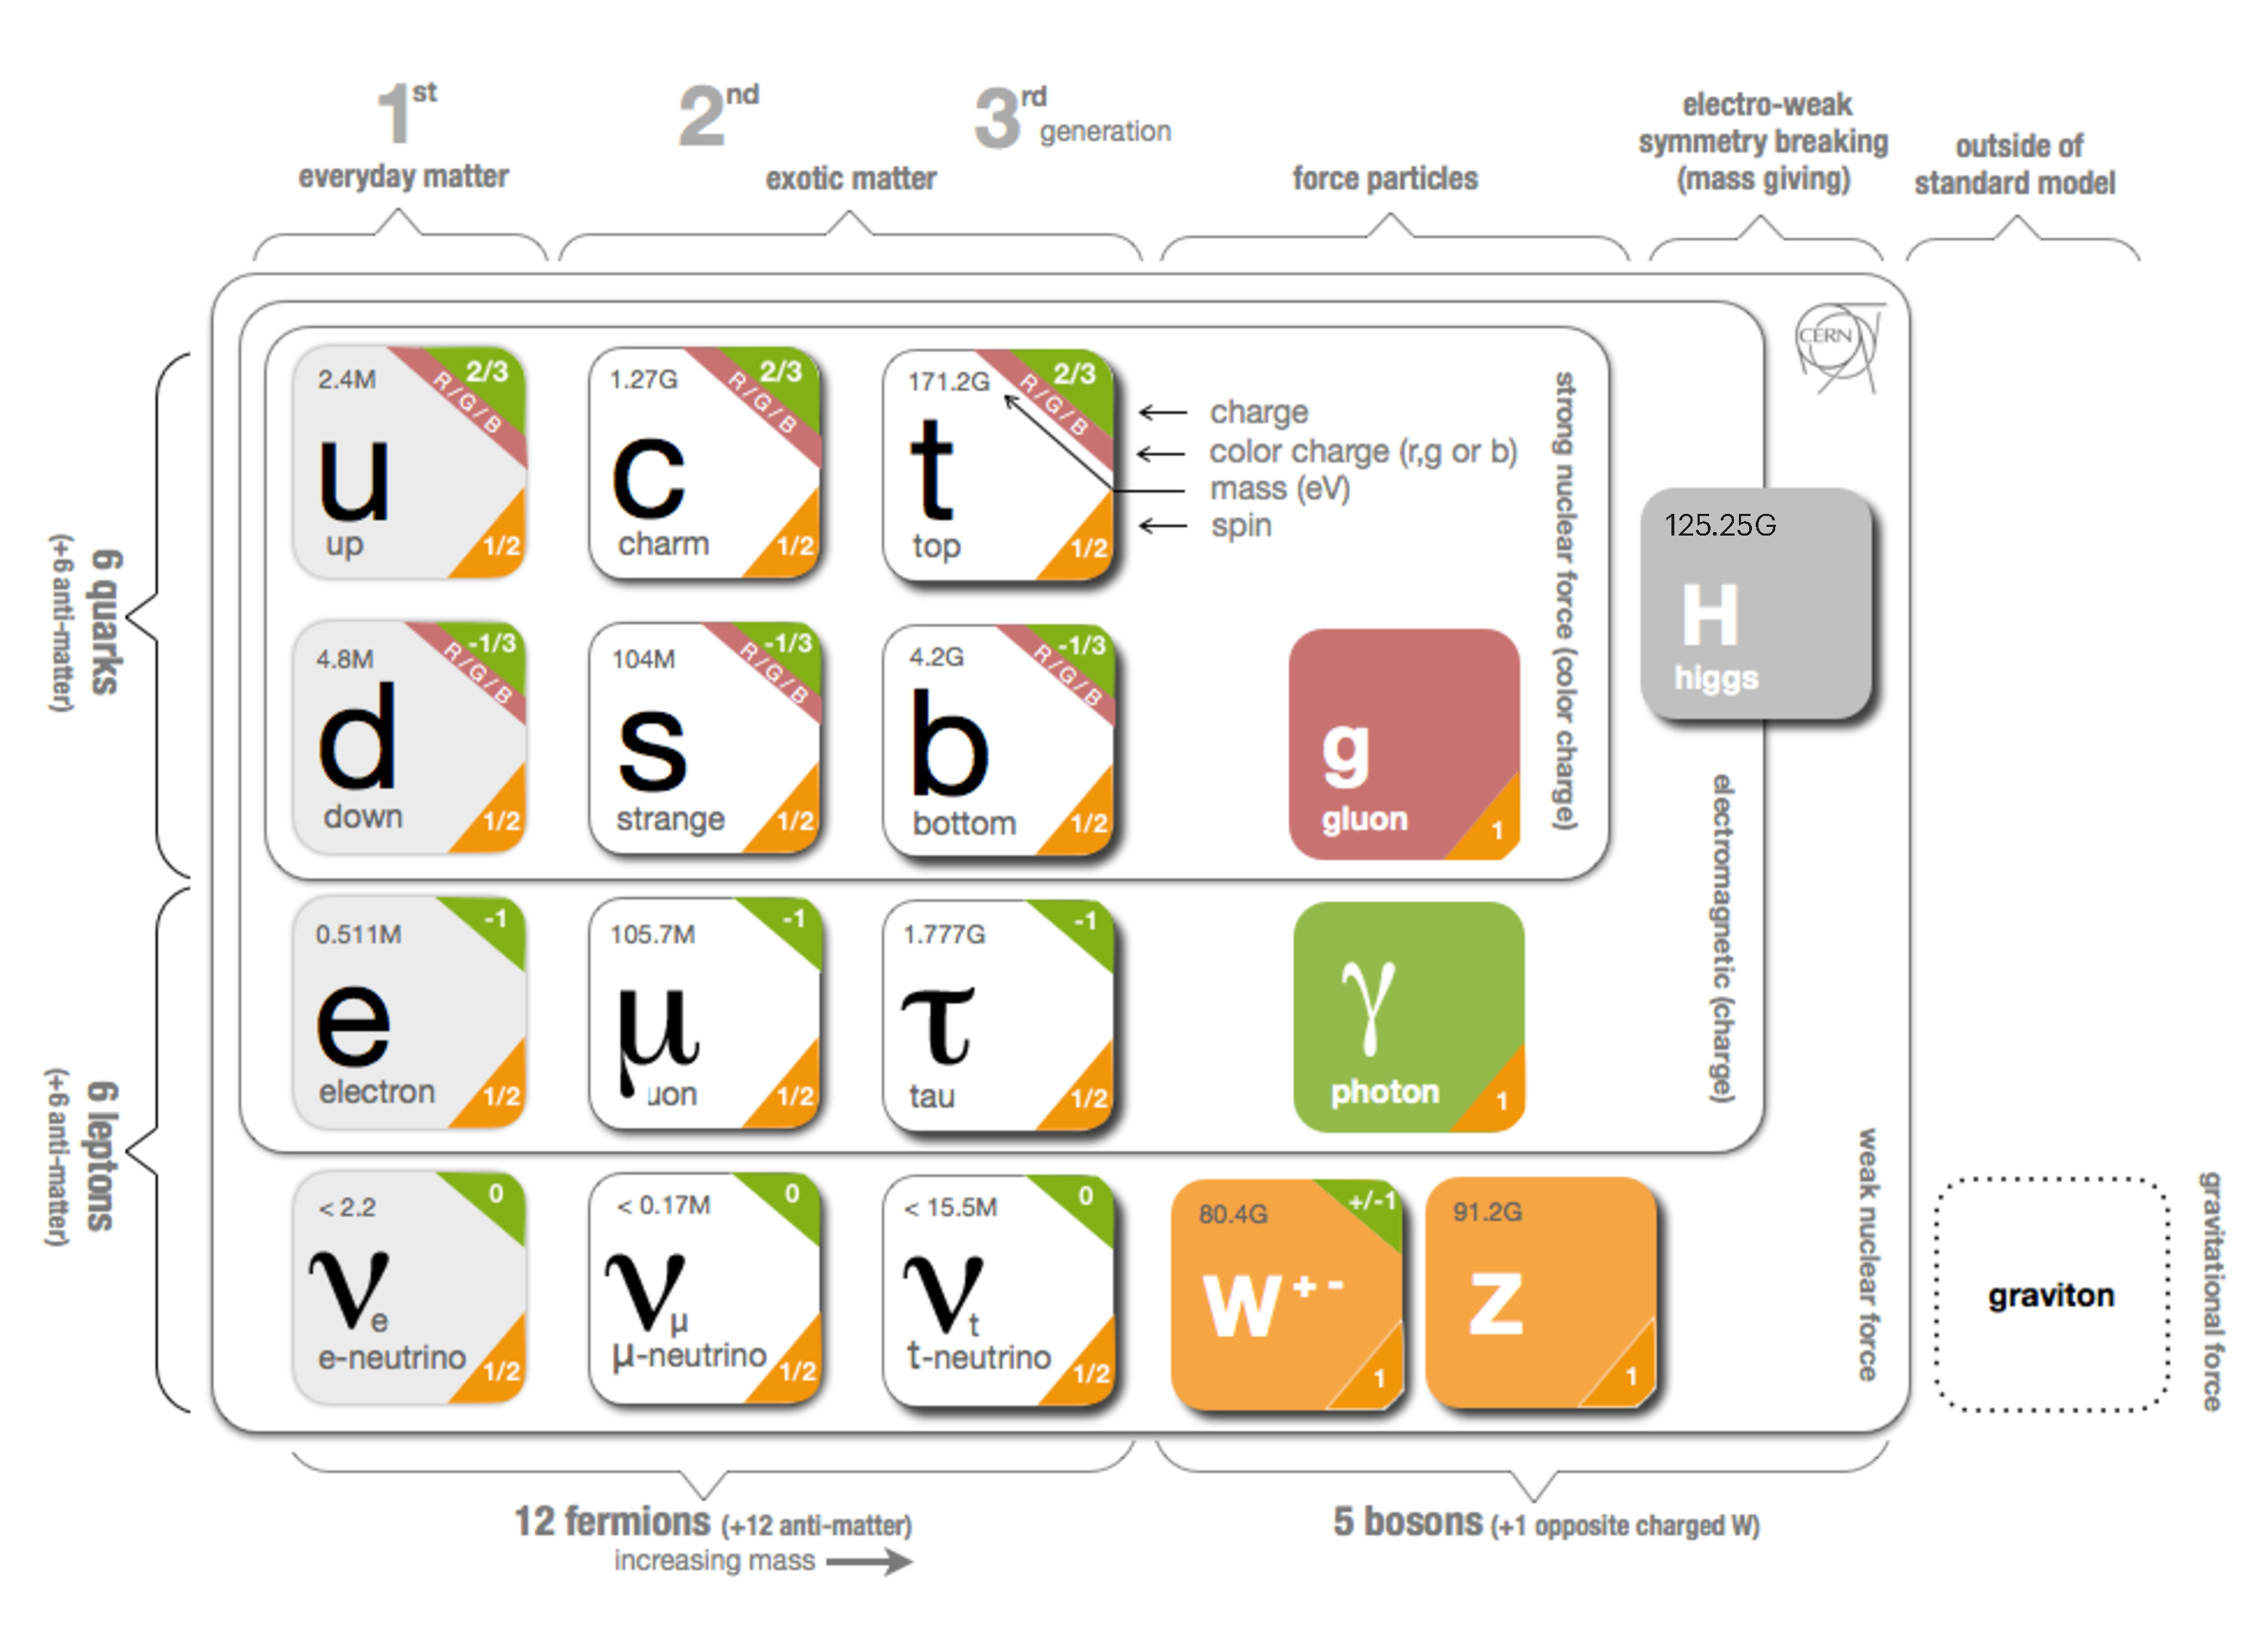
\includegraphics[width = 1\textwidth]{Chapter1/SMofElementaryParticles_fancy_modified}
    \caption{Fundamental particles of the SM (image taken and then modified from Reference~\cite{Purcell:1473657}). }
    % In each box the upper-left corner express the mass in eV, the upper-right the electric charge (green) and possible colour charges (red), and the lower-right the spin.}
    \label{fig:Chap1:SM}
\end{figure}




The SM is a gauge theory based on the symmetry group $SU(3)_\text{C} \bigotimes SU(2)_{\text{L}} \bigotimes U(1)_{\text{Y}}$, which
describes all fundamental interactions except the gravitational force\footnote{The gravitational interaction is described by Einstein's General Relativity (GR)~\cite{Einstein:1916vd}.}.
This theory provides a description for the strong, weak and electromagnetic interactions via the exchange of the corresponding
vector\footnote{``Vector bosons'' refer to all particles that have spin 1 in contrast to the ``scalar bosons'' which have spin 0.} bosons (spin-1 gauge fields).
The mediation for the electromagnetic interaction (explained in Section~\ref{sec:chap1:QED}) 
is done by one massless photon (\Pgamma).  This force is invariant under the $U(1)$ symmetry group.
While for the weak interaction, guided by $SU(2)$, three massive bosons,
\PWplus, \PWminus and \PZ, act as mediators (with masses 
$m_{\PWpm}= 80.385 \pm 0.015$~GeV~\cite{ATLAS:2017rzl} and 
$m_{\PZ}=  91.1876 \pm 0.0021$~GeV~\cite{ALEPH:2005ab}). 
Although the electromagnetic and weak interactions seem completely different at low energies, they are two aspects of the same force and
can be described simultaneously by the $SU(2)_\text{L} \bigotimes U(1)_\text{Y}$ 
symmetry group, which represents the so called electro-weak (EW) sector (detailed in Section~\ref{sec:chap1:EW}).
The strong force, with its eight massless gluons (\Pgluon), is described by the $SU(3)_\text{C}$ colour group (see Section~\ref{sec:chap1:QCD}). 
All these interactions differ in their magnitude, range and the physical phenomena that they describe. These features
are summarised in Table~\ref{tab:Chap1:FundamentalInteractions}, where 
not only the interactions described by the SM are included but the
gravitation is shown as well for completeness.  

Apart from the vector bosons, there is one massive scalar boson, the
 Higgs boson (with mass $\mH = 125.25\pm0.17$~GeV~\cite{Workman:2022ynf}). %~\cite{pdgHiggs}
Through the interaction with this particle, all massive particles of Figure 
\ref{fig:Chap1:SM} gain their masses via the EW spontaneous symmetry breaking.
This mechanism was first described by F. Englert, R. Brout~\cite{PhysRevLett.13.321} 
and P.W. Higgs~\cite{PhysRevLett.13.508}, and it is summarised in Section 
\ref{sec:chap1:ParticleMasses:HiggsMechanism}. 
% Gauge theory: A type of field theory in which the Lagrangian (and hence the dynamics of the system itself) does not 
% change (is invariant) under local transformations according to certain smooth families of operations 

\begin{table}[]
\centering
\begin{tabular}{l c c c c c}
\toprule
%Interaction & \begin{tabular}[c]{@{}l@{}}Mediator\\ boson\end{tabular} & Theory & \begin{tabular}[c]{@{}l@{}}Relative \\ stregth\end{tabular} & Range (m) \\ \midrule
Interaction     		& Theory  			& Mediator             	& Relative strength 	& Range (m) 	\\ \midrule
Strong          		& QCD	 		& $\Pgluon$              	& 1                		& $10^{-15}$    \\
Electromagnetic 	& QED/EW 		& $\Pgamma$          	&  1/137                	& $\infty$         	\\
Weak            		& EW   			& $\PWpm$, $\PZ$	&  $10^{-6}$              & $10^{18}$      \\
Gravitational     		& GR       			& -		 		&  $6\times10^{-39}$	& $\infty$  	\\ \bottomrule          
\end{tabular}
\caption{Typical strength of the fundamental interactions with respect to the strong interaction. Here the strength is understood as the coupling constant or gauge coupling parameter. 
%The description of the electromagnetism and weak interactions is unified by the EW interaction.
In GR the gravitational interaction is not a force but the effect of the four-dimensional spacetime curvature and, hence, it has no mediator in this formalism.}
\label{tab:Chap1:FundamentalInteractions}
\end{table}


%There are two important and distinct SU(3) symmetries that are relevant for the strong interactions: 
%SU(3) colour symmetry of the quark and gluon dynamics and SU(3) flavour symmetry of light quarks. 
%Each of these symmetries refers to an underlying threefold symmetry in strong interaction physics.

%A representation of the fundamental particles that compose the SM is presented in Figure~\ref{fig:Chap1:SM}.
%It is necessary to take into account that all quarks and leptons have their analogous antiparticles.% and 
% that the quarks and gluons carry the colour charge\footnote{Antiquarks carry the anti  charge}. Therefore, a more complete illustration
%of the complete set of fundamental is displayed in Figure~\ref{fig:Chap1:SM_color}, where appear the colour variations and the antiparticles
%for all the particles in Figure~\ref{fig:Chap1:SM}. The origin of the colour charge is discussed in Section~\ref{sec:chap1:QCD}.

%\begin{figure}
%    \centeringring
%   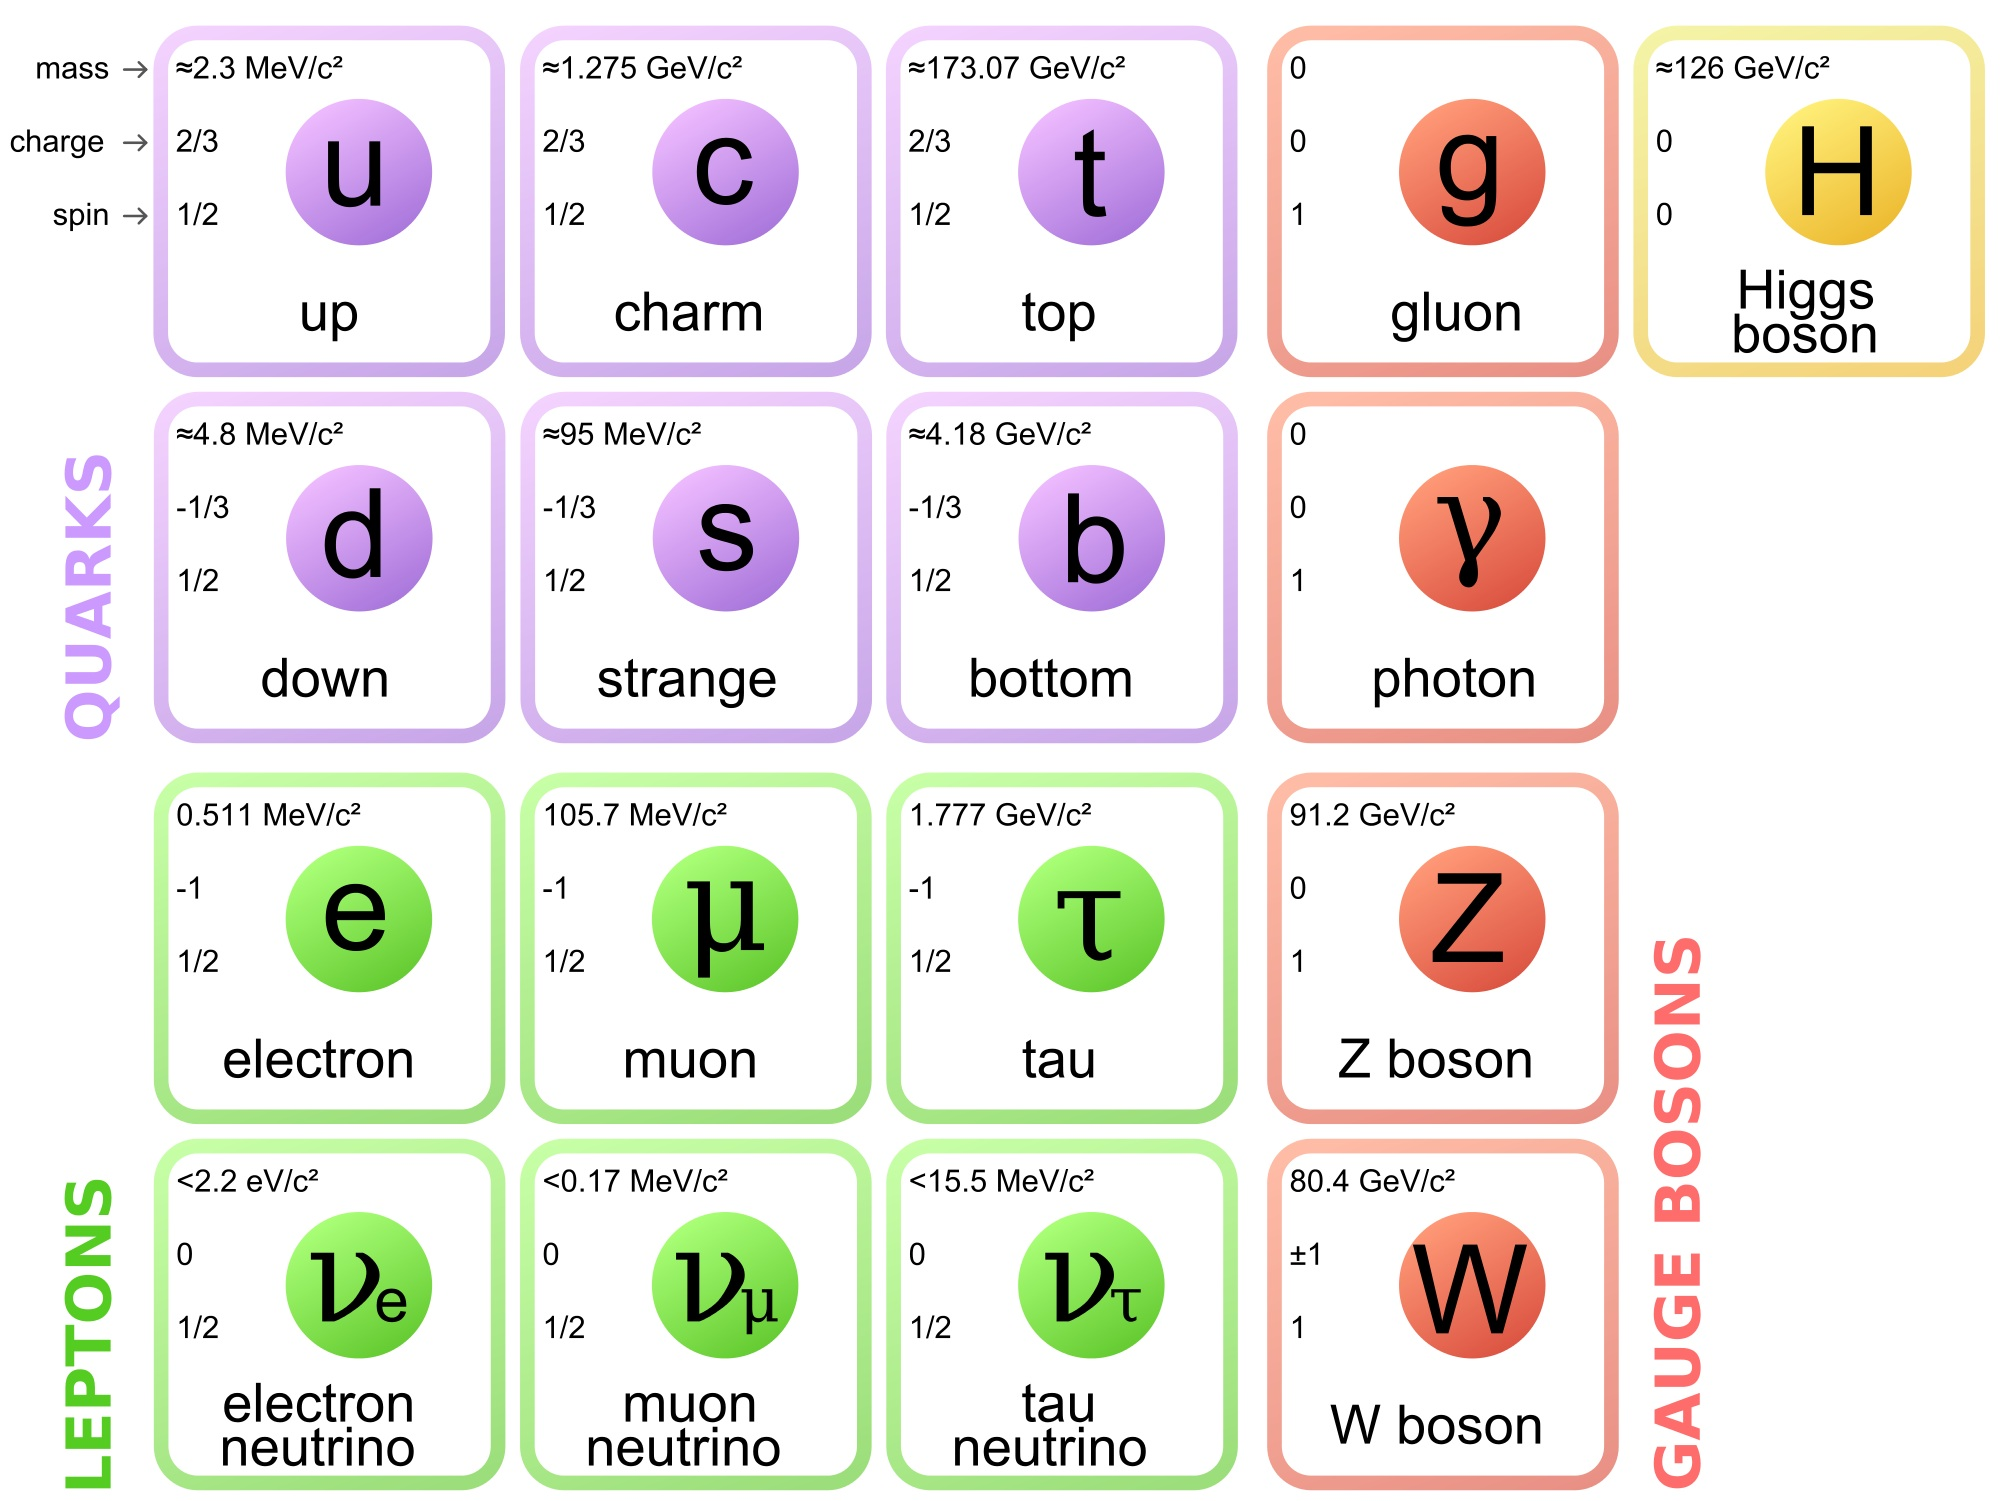
\includegraphics[width = 0.75\textwidth]{Chapter1/SMofElementaryParticles}
%  \caption{Fundamental particles of the Standard Model}
%    \label{fig:Chap1:SM_basic}
%\end{figure}


Before describing the fundamental interactions of the SM in the QFT formalism, it is convenient to introduce 
the two main types of particles according to their spin, i.e. their intrinsic angular momentum: fermions and bosons.

% FERMIONS
\paragraph{Fermions}\mbox{}\\
The fermions are the particles that follow the Fermi--Dirac statistics, i.e. obey the Pauli exclusion principle~\cite{10230794692Dirac}, resulting 
in a distribution of particles over energy levels in which two elements with the same quantum numbers cannot occupy the same states.
The fermions include all particles with half-integer spin: quarks, leptons and baryons.
A baryon is a non-fundamental particle composed of an odd number of valence quarks. 
%\footnote{The hadrons (baryons are mesons) are understood as a sea of partons being the valence quarks those which are more probable to be found in the hadron according to the parton distribution functions.} (consequently having half-integer spin)
%and nearly all matter that
%may be encountered or experienced in everyday life is baryonic matter. Protons and neutrons are examples of baryons.

%Some examples of baryons are\footnote{Between round brackets, the valence quarks are shown.} the proton (\Pup\Pup\Pdown), the 
%neutron (\Pdown\Pdown\Pup), \PLambda (\Pup\Pdown\Pstrange), \PLambdac (\Pup\Pdown\Pcharm) and \PSigmaplus (\Pup\Pup\Pstrange).
%\PDelta (\Pup \Pup \Pdown) The difference between de \PDelta and the proton is the arrangement of the spin of the quarks, 
%Apart from the 3-quark baryons, an exotic pentaquark state has been observed at LHCb experiment of the LHC~\cite{LHCb:2019kea}. 


The fundamental fermionic matter is organised in the three families of leptons 
and quarks, shown also in Table~\ref{tab:Chap1:FundamentalFermions}:

\begin{center}
$\begin{bmatrix}
\Pnue & \Pup \\
\Pelectron & \Pdown 
\end{bmatrix}$
,
$\begin{bmatrix}
\Pnum & \Pcharm \\
\Pmuon & \Pstrange 
\end{bmatrix}$
,
$\begin{bmatrix}
\Pnut & \Ptop \\
\Ptauon & \Pbottom 
\end{bmatrix}$\, .
\end{center}

%where, according to QCD, each quark appears in three different colours:
These three generations, which are defined as the columns in Figure~\ref{fig:Chap1:SM}, exhibit the same kind of 
gauge interactions and they only differ in their mass~\cite{Salam:1968rm}. %~\cite{Pich:2007vu}.
According to the EW symmetry, each family can be classified as:
\begin{center}
$\begin{bmatrix}
\Pnulepton & \ensuremath{\Pquark_{u}} \\
\Pleptonminus & \ensuremath{\Pquark_{d}} 
\end{bmatrix}$
$\equiv$
$\begin{pmatrix}
\Pnulepton \\
\Pleptonminus
\end{pmatrix}_{L}$ ,
$\begin{pmatrix}
\ensuremath{\Pquark_{u}} \\
\ensuremath{\Pquark_{d}} 
\end{pmatrix}_{L}$,
$\Pleptonminus_R$, $\ensuremath{\Pquark_{uR}}$, $\ensuremath{\Pquark_{dR}}$ \, .
\end{center}
(plus the corresponding antiparticles) where the subindices \textit{L} and \textit{R} stand from left- and right-handed particles, respectively. 
This structure responds to the fact that left-handed particles convert differently than right-handed ones under $SU(2)$ transformations.
The left-handed fields are $SU(2)_\text{L}$ doublets and the right-handed ones $SU(2)_\text{L}$ singlets. %This difference is explained with more
%detail in Section~\ref{sec:chap1:EW}. 

%As discussed in the following sections, the weak interaction only affects left-handed particles (and right-handed antiparticles) therefore,
%since the most basic representation of $SU(2)$ is a doublet, the $\begin{pmatrix}
%\Pnulepton \\
%\Pleptonminus
%\end{pmatrix}_{L}$ element appears. The $\Pleptonminus_{R}$ exists because QED affects the charged leptons but not the neutrinos and 
%, since the representation of $U(1)$ is a singlet and this force does not differentiate between eft and right-handed particle, the $\Pleptonminus_{R}$ 
 
%makes no difference between left and right-handed particles and,
%since the charged leptons but not the nautrinos are affected by QED, only the $\Pleptonminus_{R}$ but not the $\Pnulepton_R$ exits.
%The most basic representation of SU(2) is a doublet.
%\pablo{(Why there are right and left charged leptons but only left neutrinos? First of all, because  thy are not observed in Nature 
%and, secondly because the neutrinos are neutral and, hence, its quantum numbers under SM transformations are 1,1,1, i.e. they are singlets)}

The fundamental representation of $SU(3)$ is a triplet, this is why each quark can appear in three different colours, whereas each antiquark can exhibit one of the corresponding ``anticolours''. 

%->. L = Left-polarisation <- Left-handed particles transform different than right handed under SU2 transformations.
%La representación más básica de su2 es un doblete
%y las de su3 son triples (red, green blue)
%Igual que hay lepton right, en el SM no hay neutrino right : In the SM, neutrinos are left handed

%-> Should I introduce the conservation of the leptonic and baryonic numbers?

% Please add the following required packages to your document preamble:
% \usepackage{multirow}

The SM fermions properties are summarised in Table~\ref{tab:Chap1:FundamentalFermions}. 
The neutrino flavour states do not correspond to 
the mass states. What happens is that each 
flavour state is a quantum mechanical combination of neutrinos of different masses and vice versa.
More details about the neutrino masses can be found in a dedicated text in Section~\ref{sec:chap1:SM_problems}.

\begin{table}[]
\centering
\begin{tabular}{lccc}
\toprule
Family                   		& Name              			& Mass [MeV]								& Charge    \\ \midrule
\multirow{6}{*}{Quarks} 	& Up 	 ($\Pup$)                	& $2.16^{+0.49}_{-0.26}$    					& 2/3  \\
                         			& Down     ($\Pdown$)            	& $4.67^{+0.48}_{-0.17}$	 		    			& -1/3  \\
                         			& Charm 	 ($\Pcharm$)            	& (1.27$\pm$0.02)$\times 10^{3}$					& 2/3  \\
                         			& Strange  ($\Pstrange$)          	& $93^{+11}_{-5}$     				& -1/3 \\
                         			& Top  	 ($\Ptop$)              	& $(172.76\pm0.30)\times 10^{3}$     				& 2/3 \\
                         			& Bottom   ($\Pbottom$)          	& $(4.18^{+0.03}_{-0.02})\times 10^{3}$     			& -1/3 \\ \midrule
\multirow{6}{*}{Leptons} 	& Electron  ($\Pelectron$)        	& $0.5109989461\pm0.0000000031$    	& -1   \\
                         			& Muon      ($\Pmu$)		        	& $105.6583745\pm0.0000024$     		& -1   \\
                         			& Tau          ($\Ptau$)     		& $776.86\pm0.12$					& -1   \\
                         			& Electron neutrino ($\Pnue$) 	&	-	& 0\\
                         			& Muon neutrino     ($\Pnum$)	&     	-	 & 0    \\
                         			& Tau neutrino        ($\Pnut$)  	&     	-	 & 0    \\ \bottomrule
\end{tabular}
\caption{Properties of the quarks and leptons. The electric is presented in units 
of elementary charge ($1.602 \times10^{-19}$~C). The neutrino mass eigenstates, which have a fix mass, are 
different from the flavour eigenstates. Therefore, the mass of \Pnue, \Pnum and \Pnut is not defined.}
\label{tab:Chap1:FundamentalFermions}
\end{table}

%The fundamental fermions are usually understood as the fundamental building blocks 
%of matter. However, while the building blocks are important, there is a point that 
%also has to be taken into account, the force. Without force these fermions would 
%not interact which each other. The particles that mediate these interactions are the
%gauge bosons. 


\paragraph{Bosons}\mbox{}\\
Bosons differ from fermions by obeying the Bose--Einstein statistics, thus, bosons are 
not limited to single occupancy for a determined state. In other words, the Pauli exclusion 
principle is not applied. All particles with integer spin are bosons; from the particles shown on the right columns of Figure~\ref{fig:Chap1:SM}
to the mesons. Mesons, along with baryons, are part of the hadron family, i.e. particles composed of quarks (see Section~\ref{sec:chap1:QCD}). 
The particularity of mesons is that they are formed from an equal number of quarks and antiquarks (usually one of each) bound together by strong 
interactions.  Some examples of mesons are $\pi^{\pm , 0}$, $K^{\pm , 0}$ and \PJpsi. %\Ppiplus, \Ppizero, \PKplus and \PJpsi.

%Some examples of mesons are \Ppiplus (\Pup \APdown), \Ppizero ($\frac{\Pup \APup - \Pdown \APdown}{\sqrt{2}}$), \PKplus (\Pup \APstrange) and \PJpsi(\Pcharm \APcharm).
% \Petac (\Pcharm \APcharm) and \PJpsi(\Pcharm \APcharm) have the same quark distribution composition but \Petac is a pseudoscalar and a vector.

The elementary vector bosons are the force carriers and are presented in Table~\ref{tab:Chap1:FundamentalInteractions} while the Higgs boson is a fundamental particle as well. 
%\begin{figure}
%    \centering
%    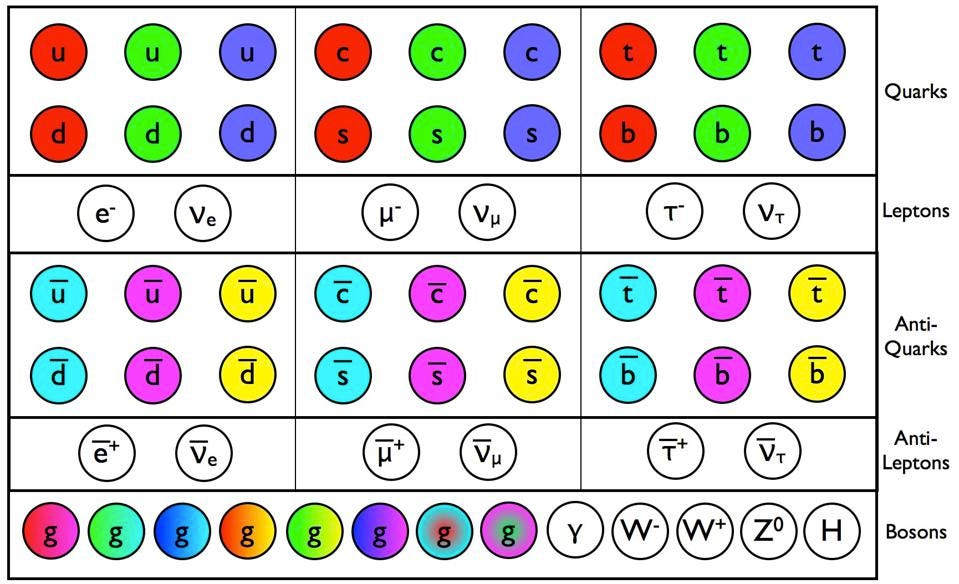
\includegraphics[width = 0.95\textwidth]{Chapter1/SM_Color}
%    \caption{Extended table of the particles composing the SM: Antiparticles and colour charge configurations are included.}
%    \label{fig:Chap1:SM_color}
%\end{figure}


%%%%%%%%%%%%%%%%%%%%%
%              Gauge Invariance                   %
%%%%%%%%%%%%%%%%%%%%%
%\paragraph{Gauge Invariance}\mbox{}\\
%Constituting one of the most successful theories of Physics, the SM is able to provide an elegant mathematical framework to
%describe the experimental physics results with great precision.
%Another key element to understand the SM is the concept of gauge invariance.
%As it is illustrated during the rest of the Section~\ref{sec:chap1:TheSM}, by demanding that 
%the Lagrange density (also denoted as Lagrangian) invariant
%under local gauge transformations, the existence of the SM force-carrier 
%bosons (\Pgamma, \PWplus, \PWminus, \PZ and \Pg). %is predicted through
%the gauge invariant field strength tensors:
%\begin{align*}
%  A  : photon
%  B  : ew
%  W : ew
%  G	 : gluon
%\end{align*}


%%%%%%%%%%%%%%%
%              QED                    %
%%%%%%%%%%%%%%%
% Peskin: http://home.ustc.edu.cn/~gengb/200923/Peskin,%20An%20Introduction%20to%20Quantum%20Field%20Theory.pdf
% notes: http://www.freebookcentre.net/physics-books-download/Relativistic-Quantum-Field-Theory-Lecture-Notes-I.html
\section{Quantum electrodynamics}
\label{sec:chap1:QED}
%The gauge invariance refers to the invariance of a theory under transformations 
%which the theory is said to posses internal symmetry.
%The transformations which are applied in all space-time locations simultaneously 
%are known as ``global'' transformations while the ones that vary from one point to 
%another are ``local''. Each local symmetry is the basis of a gauge theory and requires 
%the introduction of its own gauge bosons as it is discussed in the following pages.

In QFT, particles are described as excitations of quantum fields that satisfy the corresponding mechanical field equations.
The Lagrangians in QFT are used analogous to those of classical mechanics, where the equation of motion can be derived from the Lagrangian density
function ($\mathcal{L}$) and the Euler--Lagrange equations for fields:
\begin{equation*}
\frac{\partial\mathcal{L}}{\partial \phi} - \partial_{\mu} \frac{\partial\mathcal{L}}{\partial (\partial_{\mu} \phi)} = 0 ,
\end{equation*}
where  $\partial_{\mu} = \frac{\partial}{\partial x^{\mu}}$ denotes the partial derivatives with respect to the four-vector $x^{\mu}$ and 
$\phi = \phi(\overrightarrow{x},t)$ is the quantum field of a given fermion or boson. % A continuous quantity with a value at each point in space-time.
The Lagrangian is used to express the dynamics of the quantum field. In QFT, Noether's theorem~\cite{Noether1918}
relates a symmetry in the $\mathcal{L}$ to a conserved current. %Classical physics
%examples of how the symmetries leads to conserved quantities are:
%\begin{itemize}
%	\item Invariance under change of time $\rightarrow$ Conservation of energy
%	\item Invariance under translation in space $\rightarrow$ Conservation of momentum
%	\item Invariance under rotation $\rightarrow$ Conservation of angular momentum
%\end{itemize}

The Dirac equation, $(i \gamma^{\mu}\partial_{\mu} - m)\Psi(x)=0$, is one of the simplest relativistic field equations. Its Lagrangian
describes a free Dirac fermion:

\begin{equation}\label{eq:chap1:Dirac1}
\mathcal{L}_{0} = i \bar{\Psi}(x) \gamma^{\mu} \partial_{\mu} \Psi(x) - m \bar{\Psi}(x) \Psi(x) ,
\end{equation}
being $\Psi$ and $\bar{\Psi}$ the wave function of the particle and its hermitic conjugate, $\gamma^{\mu}$ 
are the Dirac matrices and $m$ the rest-mass of the fermion.
% In the limit m->0 Dirac equation reduces to the Weyl equation
%The gamma matrices build a set of orthogonal basis vectors for covariant vectors in a Minkowski space.
The first term of $\mathcal{L}_{0}$ is the kinetic term while the second is the mass term. 

%This Lagrangian is invariant under $U(1)$ global transformations such as:
%\begin{equation}\label{eq:chap1:DiracGlobalTransformation}
%\Psi(x) \xrightarrow{\text{U(1)}} \Psi'(x) \equiv exp\{ i Q \theta \} \Psi(x),
%\end{equation}
%where $Q \theta$ is a real constant. The phase of $\Psi(x)$ is a pure convention-dependent quantity without a physical meaning since  the observables depend on $|\Psi(x)|^{2}$.


%However, if $\theta$ was $x$ dependent, the transformation \ref{eq:chap1:DiracGlobalTransformation} would be:
%\begin{equation}\label{eq:chap1:qedLocalTransf}
%\Psi(x) \xrightarrow{\text{U(1)}} \Psi'(x) \equiv exp\{ i Q \theta (x) \} \Psi(x),
%\end{equation}
%which is not longer a global transformation but a local
%transformation instead. The transformation in \ref{eq:chap1:qedLocalTransf} would not let the $\mathcal{L}_{0}$ in \ref{eq:chap1:Dirac1} 
%invariant because the derivative in the kinetic term would go as:
%\begin{equation}\label{eq:chap1:derivativeTransformation}
%\partial_{\mu}\Psi(x) \xrightarrow{\text{U(1)}} exp\{ i Q \theta \} (\partial_{\mu} + iQ\partial_{\mu}\theta)\Psi(x).
%\end{equation}

%The gauge principle is the requirement that the $U(1)$ phase invariance should hold locally.
%In order to do so, it is necessary to introduce an additional term to the Lagrangian so that when one applies $\Psi'(x) \equiv exp\{ i Q \theta (x) \} \Psi(x)$, 
%the $\partial_{\mu}\theta$ term is canceled in \ref{eq:chap1:derivativeTransformation}.
%To achieve this invariance, a term with the vector gauge field $A_{\mu}$ is inserted. This field transforms as
%\begin{equation}\label{eq:chap1:AmuTransformation}
%A_{\mu}(x) \xrightarrow{\text{U(1)}} A_{\mu}'(x) \equiv A_{\mu}(x)+\frac{1}{e}\partial_{\mu}\theta
%\end{equation}
%with a new $D_{\mu}$, which acts as follows:  %covariant derivative:
%\begin{equation}\label{eq:chap1:NewQEDderivative}
%D_{\mu} \Psi(x) \equiv [ \partial_{\mu} + ieQA_{\mu}(x)]\Psi(x)
%\end{equation}
%which transforms like the field:
%\begin{equation*}\label{eq:chap1:QED_DerivativeTransformation}
%D_{\mu} \Psi(x) \xrightarrow{\text{U(1)}} (D_{\mu} \Psi)'(x) \equiv  exp\{ i Q \theta \} D_{\mu}\Psi(x).
%\end{equation*}

The gauge principle requires that the $U(1)$ phase invariance should hold locally. To satisfy
this, the Lagrangian density for quantum electrodynamics (QED) can be defined by replacing the partial derivatives in $\mathcal{L}_{0}$ (equation~\ref{eq:chap1:Dirac1}) with the covariant derivatives: %in \ref{eq:chap1:NewQEDderivative}:
\begin{equation}\label{eq:chap1:Dirac2}
\begin{split}
	\mathcal{L}_{\text{QED}} &\equiv i \bar{\Psi}(x) \gamma^{\mu} D{\mu} \Psi(x) - m \bar{\Psi}(x) \Psi(x) \\
				&=  i \bar{\Psi}(x) \gamma^{\mu} [ \partial_{\mu} + ieQA_{\mu}(x)] \Psi(x) - m \bar{\Psi}(x) \Psi(x) \\
				%&=  i \bar{\Psi}(x) \gamma^{\mu} \partial_{\mu} \Psi(x) -\bar{\Psi}(x) \gamma^{\mu}eQA_{\mu}\Psi(x)   - m \bar{\Psi}(x) \Psi(x) \\
				&= \mathcal{L}_{0} - eQA_{\mu}\bar{\Psi}(x)\gamma^{\mu}\Psi(x).
\end{split}
\end{equation}

The covariant derivative $D_{\mu}= \partial_{\mu} + ieQA_{\mu}(x)$ is defined this way to ensure gauge invariance. 
Here, $A_{\mu}$ is a gauge vector field that transforms like this:
 $A_{\mu}(x) \xrightarrow{\text{U(1)}} A_{\mu}'(x) \equiv A_{\mu}(x)+\frac{1}{e}\partial_{\mu}\theta$ 

Therefore, the Lagrangian in equation~\ref{eq:chap1:Dirac2} is invariant under $U(1)$ local transformation. 
%When the conversions \ref{eq:chap1:qedLocalTransf} and 
%\ref{eq:chap1:AmuTransformation} take place, the effects of the transformation are canceled out. 
Along with the original Lagrangian in equation~\ref{eq:chap1:Dirac1}, the $\mathcal{L}_{\text{QED}}$ has an additional term describing the interaction 
between the fermion $\Psi$ and the gauge field $A_{\mu}$ with a strength proportional to the charge $eQ$. 
This term, $eQA_{\mu}\bar{\Psi}\gamma^{\mu}\Psi$, which has been generated only by demanding the gauge invariance
under $U(1)$, is not other than the vertex of QED. %(Figure~\ref{fig:Chap1:QED_Vertex}). 
%\begin{figure}
%    \centering
%    \includegraphics[width = 0.35\textwidth]{Chapter1/QED_vertex}
 %   \caption{Three-point interaction vertex of QED.}
 %   \label{fig:Chap1:QED_Vertex}
%\end{figure}

This new $A_{\mu}$ term is the electromagnetic field and its quanta is the photon.
A mass term containing $A^{\mu}A_{\mu}$ is forbidden because it would violate the $U(1)$ local invariance. 
Consequently, the mediator of the new $A_{\mu}$ field, the photon, is predicted to be a massless particle. 
To make $A_{\mu}$ a propagating field it is necessary to add the kinetic term of the field $A_{\mu}$:
\begin{equation}\label{eq:chap1:QED_Kin}
	\mathcal{L}_{\text{kin}} \equiv - \frac{1}{4}F_{\mu \nu}(x) F^{\mu \nu}(x),
\end{equation}
where $F_{\mu \nu} \equiv \partial_{\mu} A_{\nu} -\partial_{\nu} A_{\mu}$. 
The kinetic term  $F_{\mu \nu} F^{\mu \nu}$ is already invariant under local $U(1)$ phase transformations.
%From the QED Lagrangian in \ref{eq:chap1:Dirac2} and the kinetic term in \ref{eq:chap1:QED_Kin},
%the Maxwell equations can be derived to describe electromagnetism, the infinite range\footnote{Since the photon is (predicted to be) massless, the electromagnetic interaction has an infinite range.} 
%interaction that occurs between particles with electrical charge.
The $\mathcal{L}_{\text{QED}}$  with this kinetic term is written as:
\begin{equation}\label{eq:chap1:QED_Complete}
	\mathcal{L}_{\text{QED}} =  \bar{\Psi}(x) (i  \gamma^{\mu} \partial_{\mu} - m ) \Psi(x) - eQ \bar{\Psi}(x) \gamma^{\mu}A_{\mu} \Psi(x) - \frac{1}{4}F_{\mu \nu}(x) F^{\mu \nu}(x).
\end{equation}


%%%%%%%%%%%%%%%
%          ElectroWeak            %
%%%%%%%%%%%%%%%
\section{Electroweak interaction}
\label{sec:chap1:EW}

\subsubsection{Weak interactions and symmetries}
The weak interaction is mediated by the $W^{\pm}$ and $\PZ$ massive gauge bosons. 
%$\PWplus$, $\PWminus$ and $\PZ$ massive gauge bosons.
The range of the interactions is within a scale of $\sim 10^{-18}$ m. %($m_{\PWpm} =  80.4$ GeV and $m_{\PZ} =  91.2$ GeV)
It is responsible for radioactive decays and flavour-changing\footnote{The lepton charge (also called lepton number) is conserved for every leptonic family.} decays of fermions such as the decay of 
the muon ($\Pmuon \rightarrow \Pelectron \APneutrino_{e} \Pneutrino_{\mu}$).


Another particularity of this interaction is that it is the only interaction that violates several fundamental symmetries. 
The three discrete symmetries that are fundamental for the SM formulation and always hold for the
electromagnetic and strong interactions but not for the weak interactions are:
\begin{itemize}
	\item \textbf{Charge conjugation (C)}: Replace positive quantum charges by negative charges and vice versa. %This symmetry is behind
										%the conservation of lepton number, baryon number and strangeness.
										It does not affect mass, energy, momentum or spin. Essentially, it is a 
										transformation that switches
										all particles with their corresponding antiparticles.
										%\begin{align*}
											%\mathcal{C} \ket{ \Psi} = \ket{\bar{\Psi}}
											%\mathcal{C} \Psi(\overrightarrow{r}, t) = \bar{\Psi}(\overrightarrow{r}, t)
										%\end{align*}
										 
	\item \textbf{Parity (P)}: Parity involves a transformation that changes the algebraic sign of the spatial coordinate system. 
								%It transforms a phenomenon by inverting its spatial coordinates through the origin. 
								It does not reverse time, mass, energy or other scalar quantities.
								%\begin{align*}
									%\mathcal{P}:\begin{pmatrix} x \\ y \\ z \end{pmatrix} \rightarrow \begin{pmatrix} -x \\ -y \\ -z \end{pmatrix} &&
									%\hat{\mathcal{P}} \Psi(r) = e^{i \frac{\theta}{2}} \Psi(-r)
									%\mathcal{P} \Psi(\overrightarrow{r}, t) = \Psi(-\overrightarrow{r}, t)
								%\end{align*}
	\item \textbf{Time reversal (T)}: Consists in flipping the sign of the time.
								%\begin{align*}
									%\mathcal{T}:t \rightarrow -t &&
									%\mathcal{T} \Psi (\overrightarrow{r}, t) = \Psi (\overrightarrow{r}, -t)
									%\mathcal{T} \Psi(t, \overrightarrow{x})\mathcal{T}^{-1} = \Psi(-t, \overrightarrow{x})
 								%\end{align*}
\end{itemize}

%\paragraph{\CP-symmetry}\mbox{}\\
The simultaneous combination of these three symmetries mentioned above results in the CPT symmetry, a profound symmetry of QFT which is
consistent through all experimental observations~\cite{Streater:1989vi}. If CPT symmetry is conserved, particles and their respective antiparticles 
are predicted to have, for example, the same mass and lifetime. %The SM is structured on the pillars of CPT symmetry and Lorentz invariance.
Meanwhile, the P and C symmetries can be combined to create the \CP symmetry, the product of the two transformations.
The weak interaction violates P and C symmetries and the combined \CP symmetry. 
Therefore, through the CPT theorem~\cite{Bell:1955djs}, if the \CP is violated,
T is violated as well to preserve the CPT invariance~\cite{Streater:1989vi}. %This has been verified experimentally
 The \CP violation plays a fundamental role in explaining the dominance of 
 matter over antimatter in the present universe. 
% Direct \CP violation is allowed in the SM if a complex phase is present in the CKM matrix.
The ``direct'' \CP violation is a phenomenon where the same decay process has a different probability for a 
particle than for an antiparticle. The measurement of the \tHq cross-section %\footnote{The cross-section concept is 
%introduced in Section~\ref{sec:Chap1:LHC:Cross-Section}.} 
allows us to determine the possible existence of a \CP-violating 
phase as it is further discussed in Section~\ref{sec:Chap1:tHq}.


%\paragraph{Parity and Charge conjugation violation}\mbox{}\\
%\paragraph{Parity violation}\mbox{}\\
%Previously theorised by Lee and Yang~\cite{Lee:1956qn}, the confirmation of the non-conservation of $\mathcal{P}$ in weak interactions 
%arrived with the Wu experiment in 1957~\cite{Wu:1957my}. %A more detailed overview of \CP violation is developed in Section~\ref{sec:chap1:CP_Violation}.
%Studying the beta decay of the Cobalt-60, Wu and collaborators found that the neutrino 
%and the antineutrino have the relative orientations of spin and linear momentum fixed.
%The neutrino spin is always opposite to the linear momentum, this is called left-handed particles.
%Meanwhile, for the antineutrinos, the momentum is always aligned in the same direction as the spin (right-handed particles).
%This causes the weak interactions which emit neutrinos or antineutrinos to violate the conservation of parity.

%Only left-handed particles and right-handed antiparticles are sensitive to the weak force. Dirac fermion fields, $\psi$, exhibit 
%chiral symmetry and the right and left handed chiral states can be expressed as:
%\begin{align}
%	\psi_{L }(x) &= \frac{1}{2} (1-\gamma_{5})\psi (x) \equiv P_{L}  \psi (x) \\
%	\psi_{R }(x) &= \frac{1}{2} (1+\gamma_{5}) \psi (x) \equiv P_{R}  \psi (x)
%\end{align}
%with
%\begin{align*}
%	\gamma^{5} &\equiv \gamma_{5} \equiv \gamma^{0}\gamma^{1}\gamma^{2}\gamma^{3} = \begin{pmatrix} 1 & 0 \\ 0 & 1 \end{pmatrix}
%\end{align*}
%where $P_{L}$ and $P_{L}$ are known as projection operators. The last equality is valid in the Dirac representation.
%This requires a more complex structure to describe weak interactions.

%In the same year, the $\mathcal{C}$ violation was found too~\cite{PhysRev.105.1415}. \pablo{Describe how the $\mathcal{C}$ violation was discovered}


%CP VIOLATION
%\paragraph{\CP violation}\mbox{}\\
%While $\mathcal{P}$ and $\mathcal{C}$ are violated in a maximal way by the weak interactions, 
%the product of these two discrete transformations, \CP, is still a good symmetry (left-handed fermions 
%$\leftrightarrow$ right-handed fermions).  Experiences such as the Wu experiment respect the \CP 
%symmetry and, in fact, in the \CP is a symmetry of nearly all the observed phenomena. However, in 
%1964 Cronin and Fitch discovered a slight (2\%) violation of the \CP symmetry in the decays of neutral 
%kaons~\cite{Christenson:1964fg}. The \CP violation plays a fundamental role to explain the dominance of
%matter over antimatter in the present universe. More information about the matter--antimatter asymmetry
%can be found in the dedicated text in Section~\ref{sec:chap1:SM_problems}. 

%Direct \CP violation is allowed in the SM if a complex phase is present in the CKM matrix (described below).
%The ``direct'' \CP violation is a phenomenon where the same decay process has a different probability for a 
%particle than for an antiparticle. An example of strong global \CP asymmetry observed corresponds to the decay
%into two kaons and one pion. The probability of $\PBplus \rightarrow \Ppiplus \PKplus \PKminus$ is 20\% higher 
%than for $\PBminus \rightarrow \Ppiminus \PKplus \PKminus$. 

%Source: https://moriond.in2p3.fr/2022/EW/slides/5/1/6_RCardinale-v1.pdf
%source: https://home.cern/news/news/physics/largest-matter-antimatter-asymmetry-observed
%So far, $\mathcal{CPT}$ is the only symmetry that stands unviolated and, given that \CP is not, the $\mathcal{T}$ must be violated as well. %Already commented

%Quizás discutir la relevancia que tiene CP en esta tesis

\paragraph{CKM matrix}\mbox{}\\
The eigenstates that interact through weak interactions, known as ``weak eigenstates'' 
(\Pdown', \Pstrange', \Pup'), are different from the physically observed mass eigenstates 
(\Pdown, \Pstrange , \Pup). This makes possible the charged-flavour-changing-weak decays
through the Cabibbo--Kobayashi--Maskawa (CKM) matrix.
The CKM matrix, $V_{\text{CKM}}$, describes the mixing between the three generations of quarks in the SM. 
The coupling of two quarks $i$ and $j$ to a \PW boson is proportional to the CKM matrix element $V_{ij}$.
\begin{equation*}
	\begin{pmatrix} \Pdown' \\ \Pstrange ' \\ \Pup ' \end{pmatrix}  = \begin{pmatrix} 	V_{ud} & V_{us} & V_{ub} \\
																V_{cd} & V_{cs} & V_{cb} \\ 
																V_{td}  & V_{ts}  & V_{tb} \end{pmatrix}
												 \begin{pmatrix} \Pdown \\ \Pstrange  \\ \Pup  \end{pmatrix}
\end{equation*}

It is a $3 \times 3$ unitary matrix described by four independent parameters: three angles and one complex phase. 
These angles are known as the Euler angles and the phase allows the \CP violation~\cite{Chau:1984fp}. 
The largest values correspond 
to the diagonal elements of the matrix.
This implies that the processes that do not change the flavour are strongly preferred over the 
family-changing charged currents. 

%Different equivalent representations of the CKM matrix can be found in literature but the Particle Data Group recommends the standard CKM
%parameterisation:

%\begin{equation}
%V_{CKM} = 	\begin{pmatrix}	
%						c_{12}c_{13}				&                  -s_{12} c_{13}					& s_{13}e^{-i \delta_{13}} 	\\
%			-s_{12}c_{23}-c_{12}s_{23}s_{13}e^{i\delta_{13}}	& -c_{12}c_{23}-s_{12}s_{23}s_{13}e^{i\delta_{13}}	& s_{23}c_{13} 			\\
%			s_{12}s_{23}-c_{12}c_{23}s_{13}e^{e\delta_{13}}	& -c_{12}s_{23}-s_{12}c_{23}s_{13}e^{i\delta_{13}}	& c_{23}c_{13}
%			\end{pmatrix}		
%\end{equation}
%where $c_{ij} \equiv \textrm{cos}\,\theta_{ij}$ and  $s_{ij} \equiv \textrm{sin}\,\theta_{ij}$, 
%with $i$ and $j$ labelling the generations ($i,\,j \in \{1,2,3\}$).
%The angles $\theta_{12}$,  $\theta_{23}$ and  $\theta_{13}$ are known as Euler angles.  
%The complex phase $\delta_{13}$ allows the \CP violation~\cite{Chau:1984fp}.
%There are other popular parameterisations such as the Kobayashi-Maskawa one
%or the Wolfenstein one. 

%The different elements of the CKM matrix are determined experimentally and are
%summarised in Table~\ref{tab:Chap1:CKM}.
 %As can be seen in this table,  the largest values correspond to the diagonal elements of the CKM matrix.
%This implies that the processes that do not change the flavour are strongly preferred over the 
%family-changing charged currents. For instance, for the top quark, the decay to any of the three down-type 
%quarks is allowed but only $|V_{td}|^{2}\times 100\% = 0.0064\%$ of times will decay to a down quark and
% $|V_{ts}|^{2}\times 100\% = 0.14\%$ to a strange quark.
%(using lowest value of $V_{tb} within its uncertainty) $|V_{tb}|^{2} \times 100 = 97 $

%\begin{table}[]
%\centering
%\begin{tabular}{c|l l}
%\begin{tabular}{c|l }
%\toprule
%CKM element 	  & Value \\
%\midrule
%   $V_{ud}$         &   $0.9740 \pm 0.00011$	%& 	\cite{Hardy:2017G0}~\cite{Pocanic:2003pf}  									
%   	\\
%   $V_{us}$         &   $0.22650 \pm 0.00048$    	%&	\cite{PhysRevLett.41.1692}~\cite{Cabibbo:2003ea}  								
%   	\\
%   $V_{cd}$         &   $0.22636 \pm 0.0048$    		%&	\cite{FlavourLatticeAveragingGroup:2019iem}~\cite{BaBar:2014xzf}~\cite{CLEO:2009svp} 	
%   	\\
%   $V_{cs}$         &   $0.97340\pm0.011$		%&	\cite{CHORUS:2005nog}\cite{BaBar:2010ixw} ~\cite{Belle:2006idb} 					
%   	\\
%   $V_{cb}$         &   $0.04053^{+0.00083}_{-0.00061}$	    	%&	\cite{HFLAV:2019otj}\cite{Belle:2017rcc}										
%   	\\
%   $V_{ub}$         &   $0.00361^{+0.00011}_{-0.00009}$   	%&	\cite{BaBar:2011xxm}~\cite{Colquhoun:2015mfa}\cite{Bauer:2000xf}\\ %\cite{Neubert:1993um}
%  	\\ 	
%   $V_{td}$          &   $0.00854^{+0.00023}_{-0.00016}$    	%&	\cite{LHCb:2013lrq}\cite{Misiak:2015xwa}										
%   	\\
%   $V_{ts}$          &   $0.03978^{+0.00082}_{-0.00060}$  		%&	\cite{LHCb:2013lrq}\cite{Misiak:2015xwa}										
%   	\\
%   $V_{tb}$          &   $ 0.999172^{+0.000024}_{-0.000035}$ 		%&	\cite{CDF:2015gsg}\cite{CMS:2015nrd}\cite{D0:2011viq}		
%   	\\
%\bottomrule
%\end{tabular}
%\caption{Magnitude of the nine elements of the CKM matrix. The mean for the different measurements has been done by~\cite{ParticleDataGroup:2020ssz}. Note how the elements that refer to quarks of the same generation are favoured over the flavour-changing currents.}
%\pablo{Igual me he venido arriba con las referencias. Son las que daba el Particle Data Group}
%\label{tab:Chap1:CKM}
%\end{table} %source: https://pdg.lbl.gov/2021/reviews/contents_sports.html


% is currently believed that CP-violation during the early universe can account for the "excess" matter, although the debate is not settled
%The \CP violation reflects the asymmetry between matter and antimatter. \pablo{ \CP violation was found with kaon oscillations <- Cite this discovery}

%La violacion cp se debe a que hay tres familias -> la fase compleja de la matriz CKM es la única fuente de violación cp


 %CPviolation depends on the CKM matrix elements associated with weak phase and strong phase:
% page 8: https://arxiv.org/pdf/2201.02385.pdf
% CP violation in ckm matrix: https://arxiv.org/pdf/hep-ph/0406184.pdf page 7

%Due to its ability to change the flavour of quarks and leptons, the theory describing the behaviour of the weak force is the quantum flavourdynamics but
%this term is rarely used because this interaction is better understood by the EW theory.
 
%\pablo{check:~\cite{Hung:2021tmi}}


\subsection{Electroweak unification}
%After the discovery of $\mathcal{P}$ in Wu experiment, a search began to relate weak and electromagnetic interactions.
%Glashow-Salam-Weinberg model
At energies above the scale of the mass of the weak vector bosons ($E_{\text{EW}} \sim m_{Z} \sim m_{W} \sim 100\,\textrm{GeV}$), the electromagnetic 
and weak interactions are unified into the electroweak (EW) force. In other words, electromagnetism and weak interactions are simultaneously described by the symmetry group $SU(2)_{\text{L}} \bigotimes U(1)_\text{Y}$. 
The subindex $\text{L}$ refers to left-handed fields and $\text{Y}$ to the weak hypercharge, a quantum number conserved under the strong interaction.  In contrast, at low energies, these interactions are treated as independent phenomena, 
the electromagnetism is described by the QED and the weak interaction proposed by E.~Fermi.

In the EW model (i.e. Glashow--Salam--Weinberg model), two new quantum numbers  are assigned to the particles of the SM: the weak isospin ($\overrightarrow{T}$) and weak hypercharge $\text{Y}'$.
Here, the left-handed chiral states of fermions form isospin doublets ($\chi_\text{L}$) with $\text{T}_{3} = \pm 1/2$ and the right-handed form chiral states are composed of isospin singlets ($\chi_\text{R}$)  with $\text{T}_{3} = 0$.
For a particle, $\text{T}_{3}$ is the third component of the $\overrightarrow{\text{T}}$, which is related to the electric charge ($Q$) and the $U(1)$ weak hypercharge by Gell-Mann--Nishijima relation:
\begin{equation}\label{eq:chap1:EW:GMN}
	Q = \text{T}_{3} + \frac{1}{2} \text{Y}' \, .
\end{equation}
%where the hypercharge is defined defined by the strangeness, charmnes, etc etc as
%https://physics.stackexchange.com/questions/379888/are-both-gell-mann-nishijima-formulas-true-for-the-same-reason
%
Through this expression, the electromagnetic coupling and the electroweak couplings are connected.
Having $\chi_\text{L}$ with $\text{T}_{3} = \pm 1/2$ and $\chi_\text{R}$  with $\text{T}_{3} = 0$ implies that a $SU(2)$ weak interaction can rotate left-handed particles 
(i.e. convert a left-handed \Pelectron into a left-handed $\Pneutrino_{e}$ emitting a \PWminus) but cannot do the same with right-handed.

Using the gauge invariance principle it is possible to find the QED Lagrangian: %and QCD Lagrangians, 
%as it is respectively described in Sections \ref{sec:chap1:QED} and \ref{sec:chap1:QCD}.
%The free Lagrangian, as in the case of QED and QCD is:
\begin{equation}\label{eq:chap1:EW:LagrangianFree}
\begin{split}
	\mathcal{L} 	&= i \sum_{j=1}^{3} \bar{\Psi}(x) \gamma^{\mu} \partial_{\mu} \Psi(x) \\
				& = i \sum_{j=1}^{3} \bar{\chi_\text{L}}(x) \gamma^{\mu} \partial_{\mu} \chi_\text{L}(x)+  i \sum_{k=1}^{3} \bar{\chi_\text{R}}(x) \gamma^{\mu} \partial_{\mu} \chi_\text{R}(x)
\end{split}
\end{equation}
where the wave function $\Psi$ has been split into the left isospin doublets $\chi_\text{L}$ and right isospin singlets $\chi_\text{R}$. 
The indices $j$ and $k$ run over 
the three generations of the SM. 
%This Lagrangian should be invariant when a gauge transformation under the $SU(2)_{L} \times U(1)_{Y}$ symmetry group in the flavour space is applied:
%\begin{align}
%	\chi_\text{L}(x) 	&\xrightarrow{\text{$SU(2)_{L} \times U(1)_{Y}$}} \chi_\text{L}'(x) =  exp\{ i \alpha^{n} \tau_{n} \}\, exp\{ i \beta y \}\,\chi_\text{L}(x) \\
%	\chi_\text{R}(x) 	&\xrightarrow{\text{$SU(2)_{L} \times U(1)_{Y}$}} \chi_\text{R}'(x) =  exp\{ i \beta y \} \,\chi_\text{R}(x)
%\end{align}
%with $\alpha, \, \beta \in \mathds{R}$ and $n \in \{1,2,3 \}$.
%This transformation is given by the generators of $SU(2)_{L} \times U(1)_{Y}$, i.e. the Pauli matrices ($\tau_{n}$) and the weak hypercharge $y$. 
%Note that $SU(2)_L$ transformation, $exp\{ i \alpha^{n} \tau_{nu} \}$, only acts on the doublet fields. This term containing the Pauli matrices is 
%non-abelian like in QCD and, like in QCD, this leads to self-interacting terms.

%To ensure invariance under  $SU(2)_{L} \times U(1)_{Y}$, four different gauge fields have to be added (three from $SU(2)$ and one from $U(1)$).
%Four is also the correct number of gauge bosons needed to describe EW interactions: \PWplus, \PWminus, \PZ and \Pgamma.
%While the three week isospin currents couple to the triplet of vector bosons $\PW^{n}_{\mu}$ with $n \in \{1,2,3 \}$, the weak hypercharge
%couples to an isosinglet $B_\mu$.  The fields $\PW^{1}_{\mu}$ and $\PW^{2}_{\mu}$ are electrically charged whereas $\PW^{3}_{\mu}$ and $B_\mu$
%are neutral fields. 
%The EW covariant derivative is defined as:
%\begin{align}
%	D^{\mu} \chi_{\text{L}_{j}}(x)	& =  [\partial_{\mu} - i g \frac{\tau_{i}}{2}\PW^{i}_{\mu}(x)  - i g' \frac{y_j}{2}  B_{\mu}(x) ] \, \chi_{\text{L}_{j}} (x)  &&  i \in [1,2,3] 	\label{eq:chap1:EW:CovariantDerivatice1} \\
%	D^{\mu} \chi_{\text{R}_{j}}(x)	& = [\partial_{\mu} - i g' \frac{y_j}{2}  B_{\mu}(x)] \,\chi_{\text{R}_{j}}(x)		,										\label{eq:chap1:EW:CovariantDerivatice2}
%\end{align}
%where $g$ and $g'$ are the interaction couplings to $\PW^{i}_\mu$ isotriplet and the $B_{\mu}$ isosinglet.

%Using the derivatives in equation~\ref{eq:chap1:EW:CovariantDerivatice1} and \ref{eq:chap1:EW:CovariantDerivatice2}, the Lagrangian 
%in \ref{eq:chap1:EW:LagrangianInvariant} is already invariant under local $SU(2)_{L} \times U(1)_{Y}$ transformations:
%\begin{equation}\label{eq:chap1:EW:LagrangianInvariant}
%	\mathcal{L} = i \sum_{j=1}^{3} \bar{\chi_\text{L}}^{j}(x) \gamma^{\mu} D_{\mu} \chi_\text{L}^{j}(x)+  i \sum_{k=1}^{3} \bar{\chi_\text{R}}^{k}(x) \gamma^{\mu} D_{\mu} \chi_\text{R}^{k}(x) 
%\end{equation}

To ensure gauge invariance under  $SU(2)_{\text{L}} \times U(1)_{\text{Y}}$, four different gauge 
fields have to be added. % (three from $SU(2)$ and one from $U(1)$)
While three week-isospin currents couple to the triplet of vector bosons $\PW^{n}_{\mu}$ 
with $n \in \{1,2,3 \}$, the weak hypercharge couples to an isosinglet $B_\mu$.
The fields $\PW^{1}_{\mu}$ and $\PW^{2}_{\mu}$ are electrically charged 
whereas $\PW^{3}_{\mu}$ and $B_\mu$ are neutral fields. 
The EW covariant derivative is defined as:
\begin{align}
	D^{\mu} \chi_{\text{L}_{j}}(x)	& =  [\partial_{\mu} - i g \frac{\tau_{i}}{2}\PW^{i}_{\mu}(x)  - i g' \frac{y_j}{2}  B_{\mu}(x) ] \, \chi_{\text{L}_{j}} (x)  &&  i \in [1,2,3] 	\label{eq:chap1:EW:CovariantDerivatice1} \\
	D^{\mu} \chi_{\text{R}_{j}}(x)	& = [\partial_{\mu} - i g' \frac{y_j}{2}  B_{\mu}(x)] \,\chi_{\text{R}_{j}}(x)		,										\label{eq:chap1:EW:CovariantDerivatice2}
\end{align}
where $g$ and $g'$ are the interaction couplings to $\PW^{i}_\mu$ isotriplet and the $B_{\mu}$ isosinglet.
Finally, if kinetic terms for the gauge bosons are included, the EW SM Lagrangian is obtained:
\begin{equation}
\begin{split}\label{eq:chap1:EW:FinalL}
	\mathcal{L}_{\text{EW}}  =	& i \sum_{j=1}^{3} \bar{\chi_\text{L}}^{j}(x) \gamma^{\mu} D_{\mu} \chi_\text{L}^{j}(x)+  i \sum_{k=1}^{3} \bar{\chi_\text{R}}^{k}(x) \gamma^{\mu} D_{\mu} \chi_\text{R}^{k}(x) \\
					& - \frac{1}{4} W^{n}_{\mu \nu}(x)W_{n}^{\mu \nu}(x) - \frac{1}{4} B_{\mu \nu}(x)B^{\mu \nu}(x) \, ,
\end{split}
\end{equation}
where the addition of kinetic terms gives rise to cubic and quadratic self-interactions among the gauge fields.
%Note that the mass terms of the fields are forbidden to ensure local gauge invariance.
%Since the observed $\PWplus$, $\PWminus$ and $\PZ$ bosons have masses different from zero, 
%it is necessary to assume that something breaks the symmetry generating the observed masses.
%In Section~\ref{sec:chap1:ParticleMasses}, the symmetry breaking is explained.

%This Lagrangian describes the interactions between gauge vector bosons and fermions below
%\begin{align*}
%	\chi_\text{L} 	&& =  \begin{pmatrix} \Pnue \\ \Pe  \end{pmatrix}_{L} & \begin{pmatrix} \Pnum \\ \Pmu  \end{pmatrix}_{L} & \begin{pmatrix} \Pnut \\ \Ptau  \end{pmatrix}_{L} & \begin{pmatrix} \Pup \\ \Pdown  \end{pmatrix}_{L} &\begin{pmatrix} \Pcharm \\ \Pstrange  \end{pmatrix}_{L} &\begin{pmatrix} \Ptop \\ \Pbottom \end{pmatrix}_{L}   \\
%	\chi_\text{R} 	&&=	 \Pe_{R} & \Pmu_{R} & \Ptau_{R} & \Pup_{R}  \Pdown_{R} & \Pcharm_{R}  \Pstrange_{R} & \Ptop_{R}   \Pbottom_{R}
%\end{align*}
%\pablo{Esto se ve muy feo: Editar $\chi_\text{L}$ y $\chi_\text{L}$.}

The $\mathcal{L}_{\text{EW}}$ in equation~\ref{eq:chap1:EW:FinalL} can be divided in two different parts according 
to the charge of the bosons: charged currents and neutral currents.
Relating the charged currents ($\PW^{1}_{\mu}$ and $\PW^{2}_{\mu}$) to the \PWplus and \PWminus 
bosons of the SM and the neutral ($\PW^{3}_{\mu}$ and $B_\mu$) ones with the $\PZ$ and $\Pgamma$, 
it is possible to build linear combinations of the original gauge fields that define the SM bosons.

%\pablo{Reescribir a partir de aquí para que quede más bonito\\}

%Therefore, from the charged-current interactions, the $\PWplus$ and $\PWminus$ bosons 
%are:
%\begin{equation}
%	\PWpm \equiv \frac{1}{\sqrt{2}}(\PW^{1}_{\mu} \mp i\PW^{2}_{\mu})\, .
%\end{equation}

%While for the neutral-current these combinations can be defined as a rotation of the so called Weinberg 
%(or weak mixing) angle $\theta_{W}$:
%\begin{equation*}\label{eq:chap1:EW:ZmuAmu}
%		\begin{pmatrix} \PW_{\mu}^3 \\ B_\mu \end{pmatrix} \equiv
%		\begin{pmatrix} \textrm{cos} \,\theta_{W} & \textrm{sin} \,\theta_{W} \\  -\textrm{sin} \,\theta_{W} & \textrm{cos}\, \theta_{W} \end{pmatrix} \begin{pmatrix} \PZ_{\mu} \\ A_{\mu} \end{pmatrix} \, .
%\end{equation*}
%Rewriting this equation, the photon and $\PZ$-boson fields are 
%\begin{align}
%	A_{\mu}	&= B_{\mu} \textrm{cos} \,\theta_{W}+ W^{3}_{\mu}  \textrm{sin} \,\theta_{W}
%	Z_{\mu}	&= -B_{\mu} \textrm{cos} \,\theta_{W}+ W^{3}_{\mu}  \textrm{sin} \,\theta_{W} \, .
%\end{align}
%In order to ensure that this $A_{\mu}$ is the one of QED, apart from the Gell-Mann-Nishijima relation (Eq.
%\ref{eq:chap1:EW:GMN}), it is required that the couplings of the \Pgamma, \PWpm and \PZ satisfy the relation:
%\begin{equation}
%	g \, \textrm{sin} \,\theta_{W} = g' \,\textrm{cos}\, \theta_{W} = e \, .
%\end{equation}

%Within the unified EW  model, once $ \theta_{W}$ is known, the mass of $\PZ$ is specified.
%Current measurements of $ \theta_{W}$ give a value of $\textrm{sin}^{2} \theta_{W} = 0.2310 \pm 0.0005$~\cite{CMS:2018ktx}. 

%\pablo{Comentar algo el GIM mechanism y las FCNC }


There is no mass term for the bosons in the EW Lagrangian that has been obtained in 
equation~\ref{eq:chap1:EW:FinalL} by demanding the $SU(2)_{L} \times U(1)_\text{Y}$ local invariance, 
which enters in contradiction with the experimental observations for the \PW and \PZ 
bosons that indicate that $m_{Z,W}$ is $\mathcal{O}(100)$~GeV.  
The introduction of such a mass term would break the symmetry, however,  
it is possible to add the mass for the \PW and \PZ bosons without losing the properties of the symmetry. 
The method to do so is known as the Englert--Brout--Higgs mechanism
or, more commonly, just the Higgs mechanism. This mechanism is described in Section~\ref{sec:chap1:ParticleMasses}.


%SU(2) con U(1) te da los bosons de W.Z y fotón pero sin masa 
%También  dan las corrientes que se observan experimentalmente

%Tomas $SU(2) \times U(1)$ y lo rompes a través del SSB, salen los W, Z y fotón con las masas que tocan  
%Romper la simetría pero conservando la local gauge invariance. 

%Al incluir el campo de Higgs, el Lagrangiano obtenido es invariante (es invariante en escalas energéticas de EW, es decir, $m_H$ hacia arriba. 
%y por debajo de esas energías, el lagrangiano ya no es invariante ) bajo $SU(2) \times U(1)$ pero los ``estados de la teoría'' no son invariantes 
% porque el estado vacío de la teoría no permanece invariante y, por lo tanto, el resto de estados tampoco. %Lo que se hace aquí es pasa al gauge unitario,



% From EW to Higgs https://cds.cern.ch/record/475776/files/9811456.pdf

%%%%%%%%%%%%%%%
%              QCD                    %
%%%%%%%%%%%%%%%
\section{Quantum chromodynamics}
\label{sec:chap1:QCD}
The QCD theory is a QFT-based model for describing the strong interactions between 
quarks and gluons (partons). This type of interaction is responsible of 
the nuclear force, the one that acts between the protons and neutrons of atoms 
binding them together. %Without the strong force, the protons inside the nucleus 
%would push each other apart due to the electromagnetic repulsion. It also holds 
%the quarks within a hadron together. 

%%%%%%
% Quarks and Colour
%%%%%%%
\subsection{Quarks and colour}%\mbox{}\\

The QCD theory is based on the $SU(3)$ symmetry group and its name derives from the ``colour'' charge, an analogous to the electric charge of QED but for strong interactions.
The colour charge was introduced in 1964~\cite{Greenberg:1964pe} to explain how quarks could coexist within some hadrons apparently having the same 
quantum state without violating the Pauli exclusion principle. To satisfy the Fermi--Dirac statistics it is necessary to add an additional quantum number, the
colour, to the theory. Each specie of quark ($q$) may have three different colours ($q^{\alpha}$, $\alpha=$1, 2, 3): red, green, and blue.
Baryons and mesons are described then by colour singlet combinations.%:
%\begin{align*}
%B = \frac{1}{\sqrt{6}} \epsilon^{\alpha \beta \gamma} \ket{\Pquark_{\alpha}\Pquark_{\beta}\Pquark_{\gamma}} &&  M= \frac{1}{\sqrt{3}} \epsilon^{\alpha \beta} \ket{\Pquark_{\alpha}\APquark_{\beta}} \, .
%\end{align*} 

Additionally, it is postulated that all hadrons must have a global neutral colour charge, i.e. the hadrons must be ``colourless''. This assumption is known as  the
confinement hypothesis and it is made to avoid the existence of non-observed extra states with non-zero colour. It is called colour confinement because it implies
that it is not possible to observe free quarks since they carry colour charge and, hence, they have to be confined within colour-singlet combinations.
% Figure~\ref{fig:Chap1:ColourCharge}  depicts how different colours and anticolours combine to create the ``colourless'' state.

%\begin{figure}
%\centering
%\begin{subfigure}{.5\textwidth}
%  \centering
%  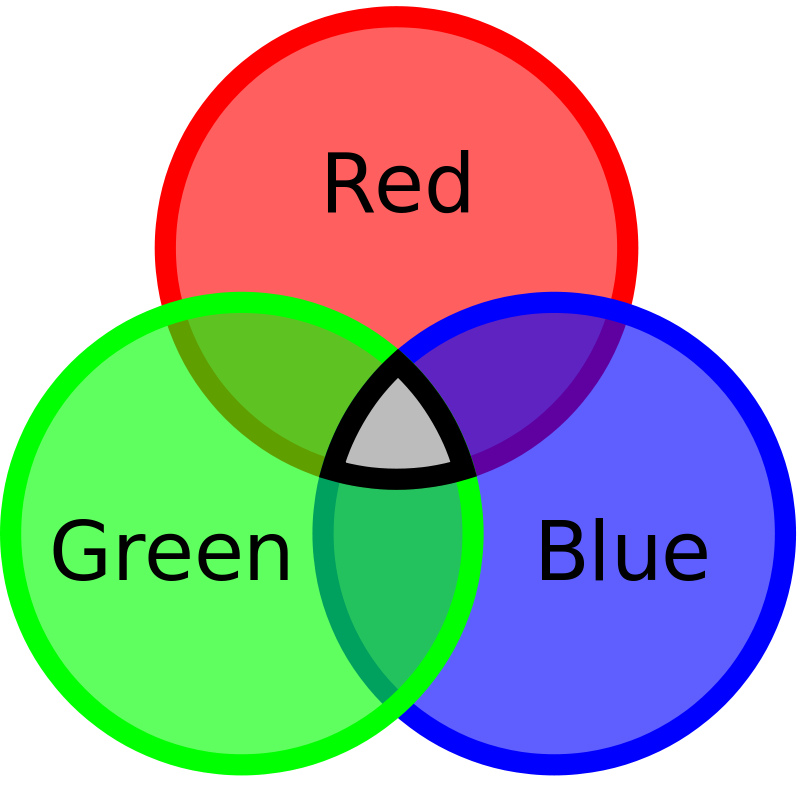
\includegraphics[width=.4\linewidth]{Chapter1/QCD-Colours.png}
%  \caption{Quark colours combine to be colourless.}
%\end{subfigure}%
%\begin{subfigure}{.5\textwidth}
%  \centering
%  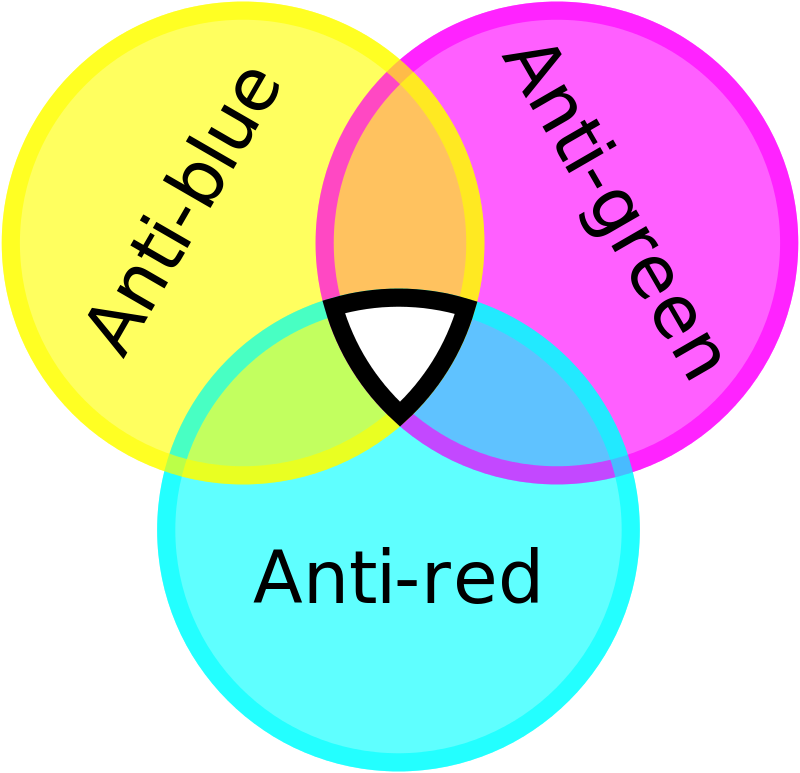
\includegraphics[width=.4\linewidth]{Chapter1/QCD-AntiColours.png}
%  \caption{Antiquark colours also combine to be colourless.}
%\end{subfigure}
%\caption{Colour charge combinations for quarks and antiquarks. Due to the confinement, the hadrons are colourless.}
%\label{fig:Chap1:ColourCharge}
%\end{figure}


%%%%%%
% % Non-Abelian gauge symmetry
%%%%%%%
% https://fse.studenttheses.ub.rug.nl/12978/1/ThesisCasperDijkstra.pdf
\subsection{Gauge invariance for \textit{SU(3)}}%\mbox{}\\
The dynamics of the quarks and gluons are controlled by the QCD Lagrangian. %Using the gauge invariance principle 
%it is possible to deduce $\mathcal{L}_{\text{QCD}}$ similarly to the reasoning developed in Section~\ref{sec:chap1:QED}.
The starting Lagrangian density is
\begin{equation}\label{eq:chap1:QCD:Lagrangian_0}
\mathcal{L}_{0} = \sum_{f} \APquark_{f}^{\alpha} (i \gamma^{\mu} \partial_{\mu} - m_{f})\Pquark_{f}^{\alpha}\, ,
\end{equation}
where $q^{\alpha}_{f}$ denotes a quark field of colour $\alpha$ and flavour $f$. The mass
of $q^{\alpha}_{f}$ is $m_f$. 

The Lagrangian in equation~\ref{eq:chap1:QCD:Lagrangian_0} has to
satisfy invariance under local transformations and hence its derivatives have to be 
substituted by covariant objects. The $SU(N)$ with $N=3$ algebra demands that there are
eight independent gauge parameters and, hence eight different gauge
bosons $G_{a}^{\mu}(x)$ are needed. With $g_{s}$ being the QCD coupling, the
covariant derivatives are:
\begin{equation*}
	D^{\mu}q_{f}^{\alpha} \equiv \big[ \partial_{\mu}  + i g_{s} \frac{\lambda^{a}}{2} G_{a}^{\mu}(x) \big] q_{f}^{\alpha} \equiv [ \partial_{\mu}  + i g_{s} G^{\mu}(x) ] q_{f}^{\alpha} \, .
\end{equation*}
In contrast to the case of QED, the non-commutativity 
of the $SU(3)_\text{C}$ matrices give rise to an additional term involving the gluon 
fields themselves: $- f^{abc}\delta \theta_{b}G_{c}^{\mu}$, with $f^{abc}$ being the
structure constant. With this, it is necessary to introduce the corresponding fields 
strengths to build a gauge-invariant kinetic terms for the gluon fields:
\begin{equation*}
	%G^{\mu \nu}		& \equiv -i\frac{-i}{g_{s}} [D^{\mu}, D^{\nu}] =  \partial_{\mu}G^{\nu} - \partial_{\nu}G^{\mu} + i g_{s}[G^{\mu},G^{\nu}] \equiv \frac{\lambda^{a}}{2}G_{a}^{\mu \nu}(x) \\
	G_{a}^{\mu \nu} \equiv \partial_{\mu}G^{\nu}_{a} - \partial_{\nu}G^{\mu}_{a} - g_{s} f^{abc} G_{b}^{\mu}G_{c}^{\nu}\, .
\end{equation*} 

Normalising the gluon kinetic term, 
the $SU(3)_\text{C}$ invariant QCD Lagrangian is obtained:
\begin{equation}
\label{eq:chap1:QCD:Lagrangian_FinalCompact}
	\mathcal{L}_{\text{QCD}} \equiv  -\frac{1}{4}G^{\mu \nu}_{a} G_{\mu \nu}^{a} + \sum_{f} \APquark_{f}^{\alpha} (i \gamma^{\mu} D_{\mu} - m_{f})\Pquark_{f}^{\alpha} \, .
\end{equation}



%Firstly, let's denote a quark field of colour $\alpha$ and flavour $f$ by $q_{f}^{\alpha}$. 
%The vector $q^{T}_{f}\equiv (q_{f}^{1}, q_{f}^{2}, q_{f}^{3})$ is defined under the $SU(3)$ colour space,  
%meaning that each dimension corresponds to a colour.
%The Lagrangian
%\begin{equation}\label{eq:chap1:QCD:Lagrangian_0}
%\mathcal{L}_{0} = \sum_{f} \APquark_{f} (i \gamma^{\mu} \partial_{\mu} - m_{f})\Pquark_{f}
%\end{equation}
%is invariant under global $SU(3)$ transformation in the colour space,
%\begin{align} \label{eq:chap1:QCD:q_trasnformation}
%q_{f}^{\alpha} \rightarrow (q_{f}^{\alpha})' = U^{\alpha}_{\beta}q^{\beta}_{\alpha}, && UU^{\dagger} = U^{\dagger}U = 1, && \textrm{det }U = 1 .
%\end{align}

%In the $SU(N)$ algebra, $SU(N)$ is the group of $N \times N$ unitary matrices ($U$) which can be written in the form $U = exp \{ i (\lambda^{a}/2) \theta_{a} \}$ with $a = 1,2,...,N^{2}-1$.
%Therefore, the SU(3) matrices can be written as
%\begin{equation}\label{eq:chap1:QCD:U_matrix}
%	U = exp \big\{ i \frac{\lambda^{a}}{2}\theta_{a} \big\}\, ,
%\end{equation}
%where the index $a$ goes from 1 to 8 for the arbitrary parameter $\theta_{a}$ and  $\frac{\lambda^{a}}{2}$, which denotes the fundamental representation of the $SU(3)$ algebra.
%The Einstein notation for summation over repeated indices is implied. The matrices $\lambda^{a}$ are traceless and satisfy the commutation relations~\cite{Pich:2007vu}:
%\pablo{Why does SU(3) has 8 gauge parameters? SU(N) is the group of $N \times N$ unitary matrices ($U$) }%For $SU(N)$  with $N=3$, the fundamental representation correspond to the eight Gell-Mann matrices.2 }
%\begin{equation} \label{eq:chap1:QCD:ConmutationSU3}
%	\big[ \frac{\lambda^{a}}{2}, \frac{\lambda^{b}}{2}\big] = i f^{abc} \frac{\lambda^{c}}{2} \, ,
%\end{equation}
%being $f^{abc}$ the $SU(3)_C$ structure constants, which are real and totally antisymmetric. 

%To satisfy the gauge invariance requirement, the Lagrangian has to be invariant under $SU(3)$ local transformations, i.e, transformations in which 
%the phase is dependent of the space-time location, $\theta_{a} = \theta_{a} (x)$. To fulfil the condition, the quark derivatives in the 
%Lagrangian in \ref{eq:chap1:QCD:Lagrangian_0} have to  be substituted by covariant objets. Since there are eight independent gauge 
%parameters, eight different gauge  bosons $G_{a}^{\mu}(x)$ are needed\footnote{The eightfold multiplicity of gluons is labeled by a combination of   and anti  charge (e.g. red--antigreen)}. 
%This bosons are the eight gluons and  the new covariant objects are:
%\begin{equation*}
%	D^{\mu}q_{f} \equiv \big[ \partial_{\mu}  + i g_{s} \frac{\lambda^{a}}{2} G_{a}^{\mu}(x) \big] q_{f} \equiv [ \partial_{\mu}  + i g_{s} G^{\mu}(x) ] q_{f} \, .
%\end{equation*}
%The compact matrix notation is used  $[G^{\mu}(x)]_{\alpha \beta} \equiv \big( \frac{\lambda^{a}}{2} \big)_{\alpha \beta} G_{a}^{\mu}(x)$.

%To ensure that the covariant derivative ($D^{\mu}q_{f}$) transforms like the $q_f$, the transformation of the gauge fields are:
%\begin{align}\label{eq:chap1:QCD:G_trasnformation}
%	D^{\mu} \rightarrow (D^{\mu})'  = UD^{\mu}U^{\dagger} && G^{\mu} \rightarrow (G^{\mu})' = UG^{\mu}U^{\dagger}+\frac{i}{g_{s}} (\partial_{\mu} U )U^{\dagger} \, .
%\end{align}
%The quark and gluon fields transform under an infinitesimal local transformation, i.e. $\theta_{a} (x) =  \delta \theta_{a}(x) \approx 0$, the $SU(3)_C$ unitary matrices (equation~\ref{eq:chap1:QCD:U_matrix}) can be expressed as their first order expansion:
%\begin{equation*}
%	U = exp \big\{ i \frac{\lambda^{a}}{2}\theta_{a}(x) \big\} \approx 1 + i \big( \frac{\lambda^{a}}{2} \big) \delta \theta_{a}(x)
%\end{equation*}
%and, consequently, the transformations for que colour-vector field (equation~\ref{eq:chap1:QCD:q_trasnformation}) and 
%gluon field (equation~\ref{eq:chap1:QCD:G_trasnformation}) become:
%\cite{Pich:2007vu},
%\begin{align*}
%	q^{\alpha}_{f}	& \rightarrow (q^{\alpha}_{f})' = q^{\alpha}_{f} + \big( \frac{\lambda^{a}}{2} \big)_{\alpha \beta} \delta \theta_{a} q_{f}^{\beta} \\
%	G_{a}^{\mu}	& \rightarrow (G_{a}^{\mu})' =  G_{a}^{\mu} - i \frac{i}{g_{s}} \partial_{\mu} (\delta \theta_{a}) - f^{abc}\delta \theta_{b}G_{c}^{\mu}.
 %\end{align*}
 
%In contrast to the transformation for the photon field in QED (equation~\ref{eq:chap1:AmuTransformation}), 
%the non-commutativity\footnote{Because the generators of $SU(3)$ do not conmute, QCD is known as 
%non-Abelian gauge theory.} of the $SU(3)_C$ matrices give rise to an additional term involving the gluon 
%fields themselves ($- f^{abc}\delta \theta_{b}G_{c}^{\mu}$), as the relation \ref{eq:chap1:QCD:ConmutationSU3} expresses.
%This transformation are more complicated than the ones of equation~\ref{eq:chap1:AmuTransformation}.
%The adjoint representation of an $SU(N)$ group is given by the $(N^{2}-1)\times(N^{2}-1)$ matrices $(\lambda^{a} / 2)_{bc} \equiv -i f^{abc}$.
%For constant $\delta \theta_{a}$, the transformation rule for the gauge fields is expressed in terms of the structure constants $f^{abc}$; 
%thus, the gluon fields belong to the adjoint representation for the colour group. 
%There is a unique coupling at $SU(3)_C$, $g_s$. All the colour-triplet flavours couple to the gluon fields with exactly the same interaction strength. 

%It is necessary to introduce the corresponding fields strengths to build a gauge-invariant kinetic terms for the gluon fields.
%\begin{align*}
%	G^{\mu \nu}		& \equiv -i\frac{-i}{g_{s}} [D^{\mu}, D^{\nu}] =  \partial_{\mu}G^{\nu} - \partial_{\nu}G^{\mu} + i g_{s}[G^{\mu},G^{\nu}] \equiv \frac{\lambda^{a}}{2}G_{a}^{\mu \nu}(x) \\
%	G_{a}^{\mu \nu}	& \equiv \partial_{\mu}G^{\nu}_{a} - \partial_{\nu}G^{\mu}_{a} - g_{s} f^{abc} G_{b}^{\mu}G_{c}^{\nu}\, .
%\end{align*} 

%Under a $SU(3)_C$ transformation,
%\begin{equation}
%	G^{\mu \nu} \rightarrow (G^{\mu \nu})' = UG^{\mu \nu}U^{\dagger}
%\end{equation}
%and the colour trace $\textrm{Tr}(G^{\mu \nu}G_{\mu \nu}) = \frac{1}{2}G^{\mu \nu}G_{\mu \nu}$ remains invariant.  Normalising the gluon kinetic term, 
%the $SU(3)_C$ invariant QCD Lagrangian is obtained:
%\begin{equation}\label{eq:chap1:QCD:Lagrangian_FinalCompact}
%	\mathcal{L}_{\text{QCD}} \equiv   -\frac{1}{4}G^{\mu \nu}_{a}G_{\mu \nu}^{a} + \sum_{f} \APquark_{f} (i \gamma^{\mu} D_{\mu} - m_{f})\Pquark_{f} \, .
%\end{equation}

Note how the gluon--gluon vertex is found by demanding the gauge invariance under local $SU(3)_\text{C}$ transformation.
A mass term is forbidden for the gluon fields by the $SU(3)_\text{C}$  gauge symmetry because a term of the form 
$\frac{1}{2}m^{2}_{G}G^{\mu}_{a}G_{\mu}^{a}$ would not be invariant.
The gluons are, then, predicted by the theory to be spin-1 massless particles.

Thanks to the colour symmetry properties, this Lagrangian looks very simple and all its interactions depend on the strong coupling
constant, $g_s$. In contrast to the Lagrangian derived for QED (see equation~\ref{eq:chap1:Dirac2}), 
in $\mathcal{L}_{\text{QCD}}$ the boson field 
has a self-interacting term. These gluon self-interactions give rise to the triple and quadratic gluon vertex.
The self-interactions among the gluon fields can explain features such as the asymptotic freedom and confinement.
%These properties were not present in QED. 
The asymptotic freedom causes interactions between particles to become asymptotically weaker as the energy 
scale increases and the corresponding length scale decreases. 
The confinement implies that the strong forces increase with the distance, therefore, 
as two colour charges are separated, at some point it becomes energetically favourable 
for a new quark-antiquark pair to appear rather than to keep getting further. These new quarks 
bond with the previous two, preventing single quarks from being isolated. This mechanism, 
depicted in Figure~\ref{fig:Chap1:colorConfinement}, explains graphically why the strong 
interaction is responsible for keeping the quarks together forming hadrons.

%\begin{figure}
%    \centering
%    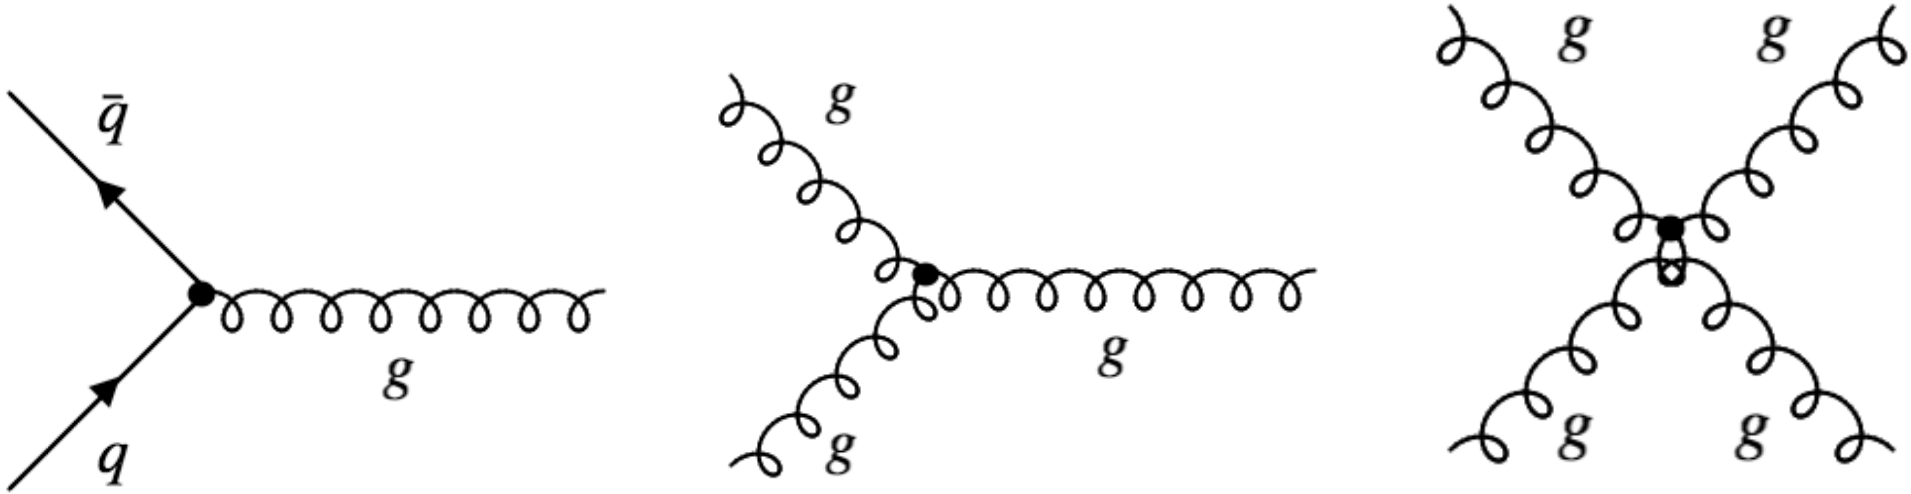
\includegraphics[width = 0.75\textwidth]{Chapter1/QCD_vertex}
%    \caption{The predicted QCD interaction vertices arising from the requirement of $SU(3)_C$ local gauge invariance. The presence of the triples and quadruple gluon vertices is possible to the Non-Abelian nature of $SU(3)_C$.}
%    \label{fig:Chap1:gluonvertex}
%\end{figure}

\begin{figure}[h]
    \centering
    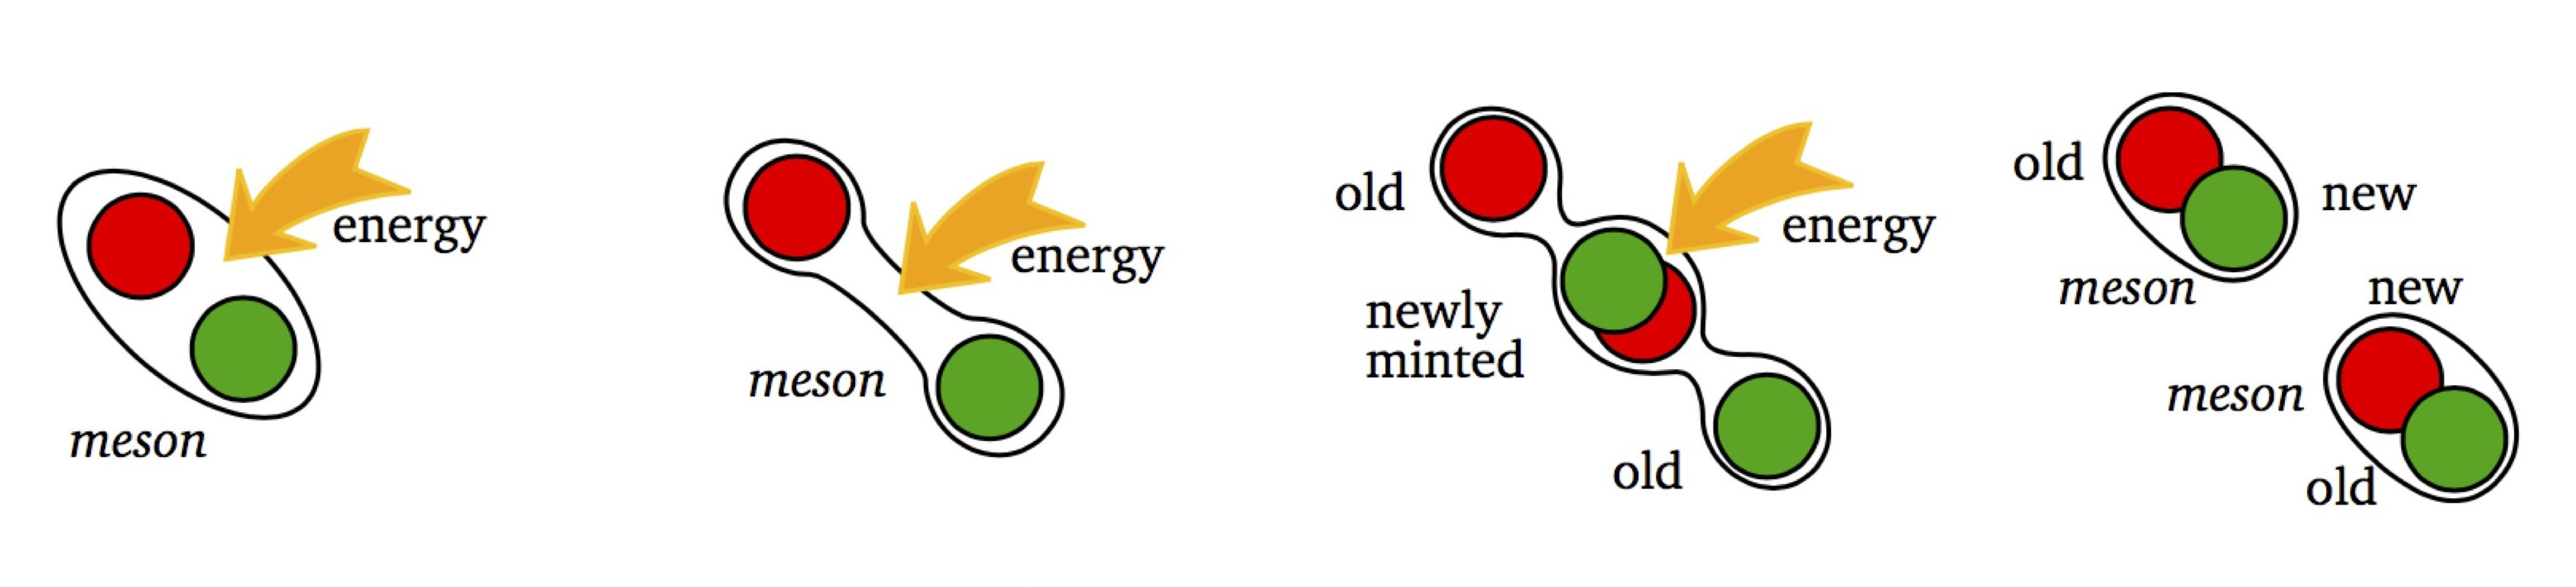
\includegraphics[width = 0.85\textwidth]{Chapter1/ConfinementQCD}
    \caption{The QCD colour confinement explains the inseparability of quarks inside a hadron despite of investing ever more energy. In this example, the mechanism is shown for a meson.}
\label{fig:Chap1:colorConfinement}\end{figure}


%\pablo{Maybe, expand the QCD Lagrangian in \ref{eq:chap1:QCD:Lagrangian_FinalCompact} and explain its different elements.}


%%%%%%%%%%%%%%%%%%%%%
%                  Particle masses                   %
%%%%%%%%%%%%%%%%%%%%%
\section{Particle masses}
\label{sec:chap1:ParticleMasses}
For the QED Lagrangian, $\mathcal{L}_{\text{QED}}$  (see equation~\ref{eq:chap1:QED_Complete}), 
it is clear how the mass of the photon must be zero in order to satisfy the $U(1)$ local gauge symmetry because,
if a mass term for the vector gauge field $A_{\mu}$ is included, the $\mathcal{L}_{\text{QED}}$ would 
be non-invariant.
%if a mass term for the vector gauge field $A_{\mu}$ is included, the $\mathcal{L}_{\text{QED}}$ would be:
%\begin{equation*}\label{eq:chap1:QED_massivephoton}
%	\mathcal{L}_{\text{QED}} =  \bar{\Psi}(x) (i  \gamma^{\mu} \partial_{\mu} - m ) \Psi(x) - eQ \bar{\Psi}(x) \gamma^{\mu}A_{\mu} \Psi(x) - \frac{1}{4}F_{\mu \nu}(x) F^{\mu \nu}(x) + \frac{1}{2}m_{\Pgamma}^{2}A_{\mu}A^{\mu}
%\end{equation*}
%and, with the $U(1)$ transformation in equation~\ref{eq:chap1:AmuTransformation}, the new mass term becomes: 
%\begin{equation*}
%	\frac{1}{2}m_{\Pgamma}^{2}A_{\mu}A^{\mu} \rightarrow \frac{1}{2}m_{\Pgamma}^{2} (A_{\mu} + \frac{1}{e}\partial_{\mu}\theta ) (A^{\mu} +\frac{1}{e}\partial^{\mu}\theta) \neq \frac{1}{2}m_{\Pgamma}^{2}A_{\mu}A^{\mu}\, .
%\end{equation*}
%Confirming that the photon mass term is not invariant under local $U(1)$ and, consequently, that the photon must be massless to satisfy the gauge invariance.
%Experimental efforts to measure the mass of the photon have set an upper limit of $m_{\Pgamma} \leq 1 \times 10^{-18} $ eV~\cite{Ryutov:2007zz}.
%Recent limits form cosmological measurements set the limit in $m_{\Pgamma} \leq 4 \times 10^{-15} $~\cite{Wei:2020wtf}.

The Lagrangian of QCD as presented in equation~\ref{eq:chap1:QCD:Lagrangian_FinalCompact} also demonstrates a similar restriction:
the mass term for the gluon fields is forbidden 
by the $SU(3)_\text{C}$ gauge symmetry. Therefore, the mediating bosons for the strong interactions are massless as well (experimentally, a mass as large as the upper limits
of a few MeV have been set, see Reference~\cite{Yndurain:1995uq}).


While the prohibition of mass terms for the bosons of QED and QCD is not a problem, 
this requirement also applies to the $SU(2)_\text{L}$.
This condition enters into open contradiction with the measurements of large masses for the
%\PW ($m_{\PW} = 80.370 \pm 0.007 \textrm{ (stat.)}\pm 0.017\textrm{ (syst.)}$ GeV~\cite{ATLAS:2017rzl}) 
%and \PZ ($m_{\PZ} = 91.1852 \pm 0.0030$ GeV~\cite{OPAL:2000ufp}) bosons of weak interactions. 
%\pablo{<- to do: Aquí no estoy utilizando las mismas medidas de la masa de $m_{\PW}$ y $m_{\PZ}$ que antes. He %de escoger una and stick to it.}
\PW and \PZ bosons of weak interactions.


For weak interactions, the problem of massless particles does not only affect the bosons. Since under the $SU(2)_\text{L}$ left-handed particles
transform as weak isospin doubles and right-handed particles as isospin singlets, the mass term of a spinor field $\Psi$ written as chiral states also
breaks the required gauge invariance.
% $-m \bar{\Psi}(x) \Psi(x) = -m \bar{\Psi}(x)(P_{R} + P_{L})\Psi(x) = -m (\bar{\Psi}_{R}(x) \Psi_{L}(x) + \bar{\Psi}_{L}(x) \Psi_{R}(x))$

The Englert--Brout--Higgs mechanism~\cite{PhysRevLett.13.321, PhysRevLett.13.508, PhysRevLett.13.585} describes how both the \PW and \PZ bosons and the fermions acquire mass without breaking the local gauge symmetry of the SM. 


%%%%%%%%%%%%%%%%%%%%%
%                  The Higgs mechanism           %
%%%%%%%%%%%%%%%%%%%%%
\subsection{The Englert--Brout--Higgs mechanism}\label{sec:chap1:ParticleMasses:HiggsMechanism}

%\paragraph{Goldstone theorem and spontaneous symmetry breaking}\mbox{}\\
%For a scalar field $\phi$ with a Lagrangian of the form:
%\begin{equation}\label{eq:chap1:HiggsMechanism:Example}
%	\mathcal{L} = \frac{1}{2}\partial_{\mu}\phi_{i}\partial^{\mu}\phi_{i} -V(\phi) \textrm{ where } V(\phi) = \frac{1}{2}\mu^{2}\phi_{i} \phi_{i} + \frac{1}{4}\lambda(\phi_{i} \phi_{i})^{2} \, .
%\end{equation}
%This Lagrangian is invariant under $\phi_{i} \rightarrow \phi_{i}'= R_{ij}\phi_{j}$, where $R_{ij}$ are rotational matrices in 4-dimensions.
% The mass term is the one with $\phi_{i} \phi_{i}$ and 
%the parameter $\lambda$ has to be positive for $\mathcal{L}$ to describe a physical system, if $\lambda$ <0 the potential is unbounded from below.
%Contrary, the parameter $\mu^{2}$ can be either positive or negative. 
%As depicted in Figure~\ref{fig:Chap1:SM:HiggsMechanism:PotentialExample:Positive}, if $\mu^{2}>0$, the vacuum expectation value 
%(i.e. minimum of potential) is located at the origin $\phi_0$ and this $\mathcal{L}$ would describe a spin-0 particle of mass $\mu$. 
%However, if $\mu^{2}<0$, the potential $V(\phi)$ has the form of Figure~\ref{fig:Chap1:SM:HiggsMechanism:PotentialExample:Positive} and $\mathcal{L}$
%would not represent anymore the Lagrangian of a particle of mass $\mu$. The vacuum expectation value is now multivalued:
%\begin{equation*}
%	\phi_{0} = \pm \sqrt{-\frac{\mu^{2}}{\lambda}} \equiv \pm v \, .
%\end{equation*}
%
%\begin{figure}
%\centering
%\begin{subfigure}{.5\textwidth}
% \centering
%  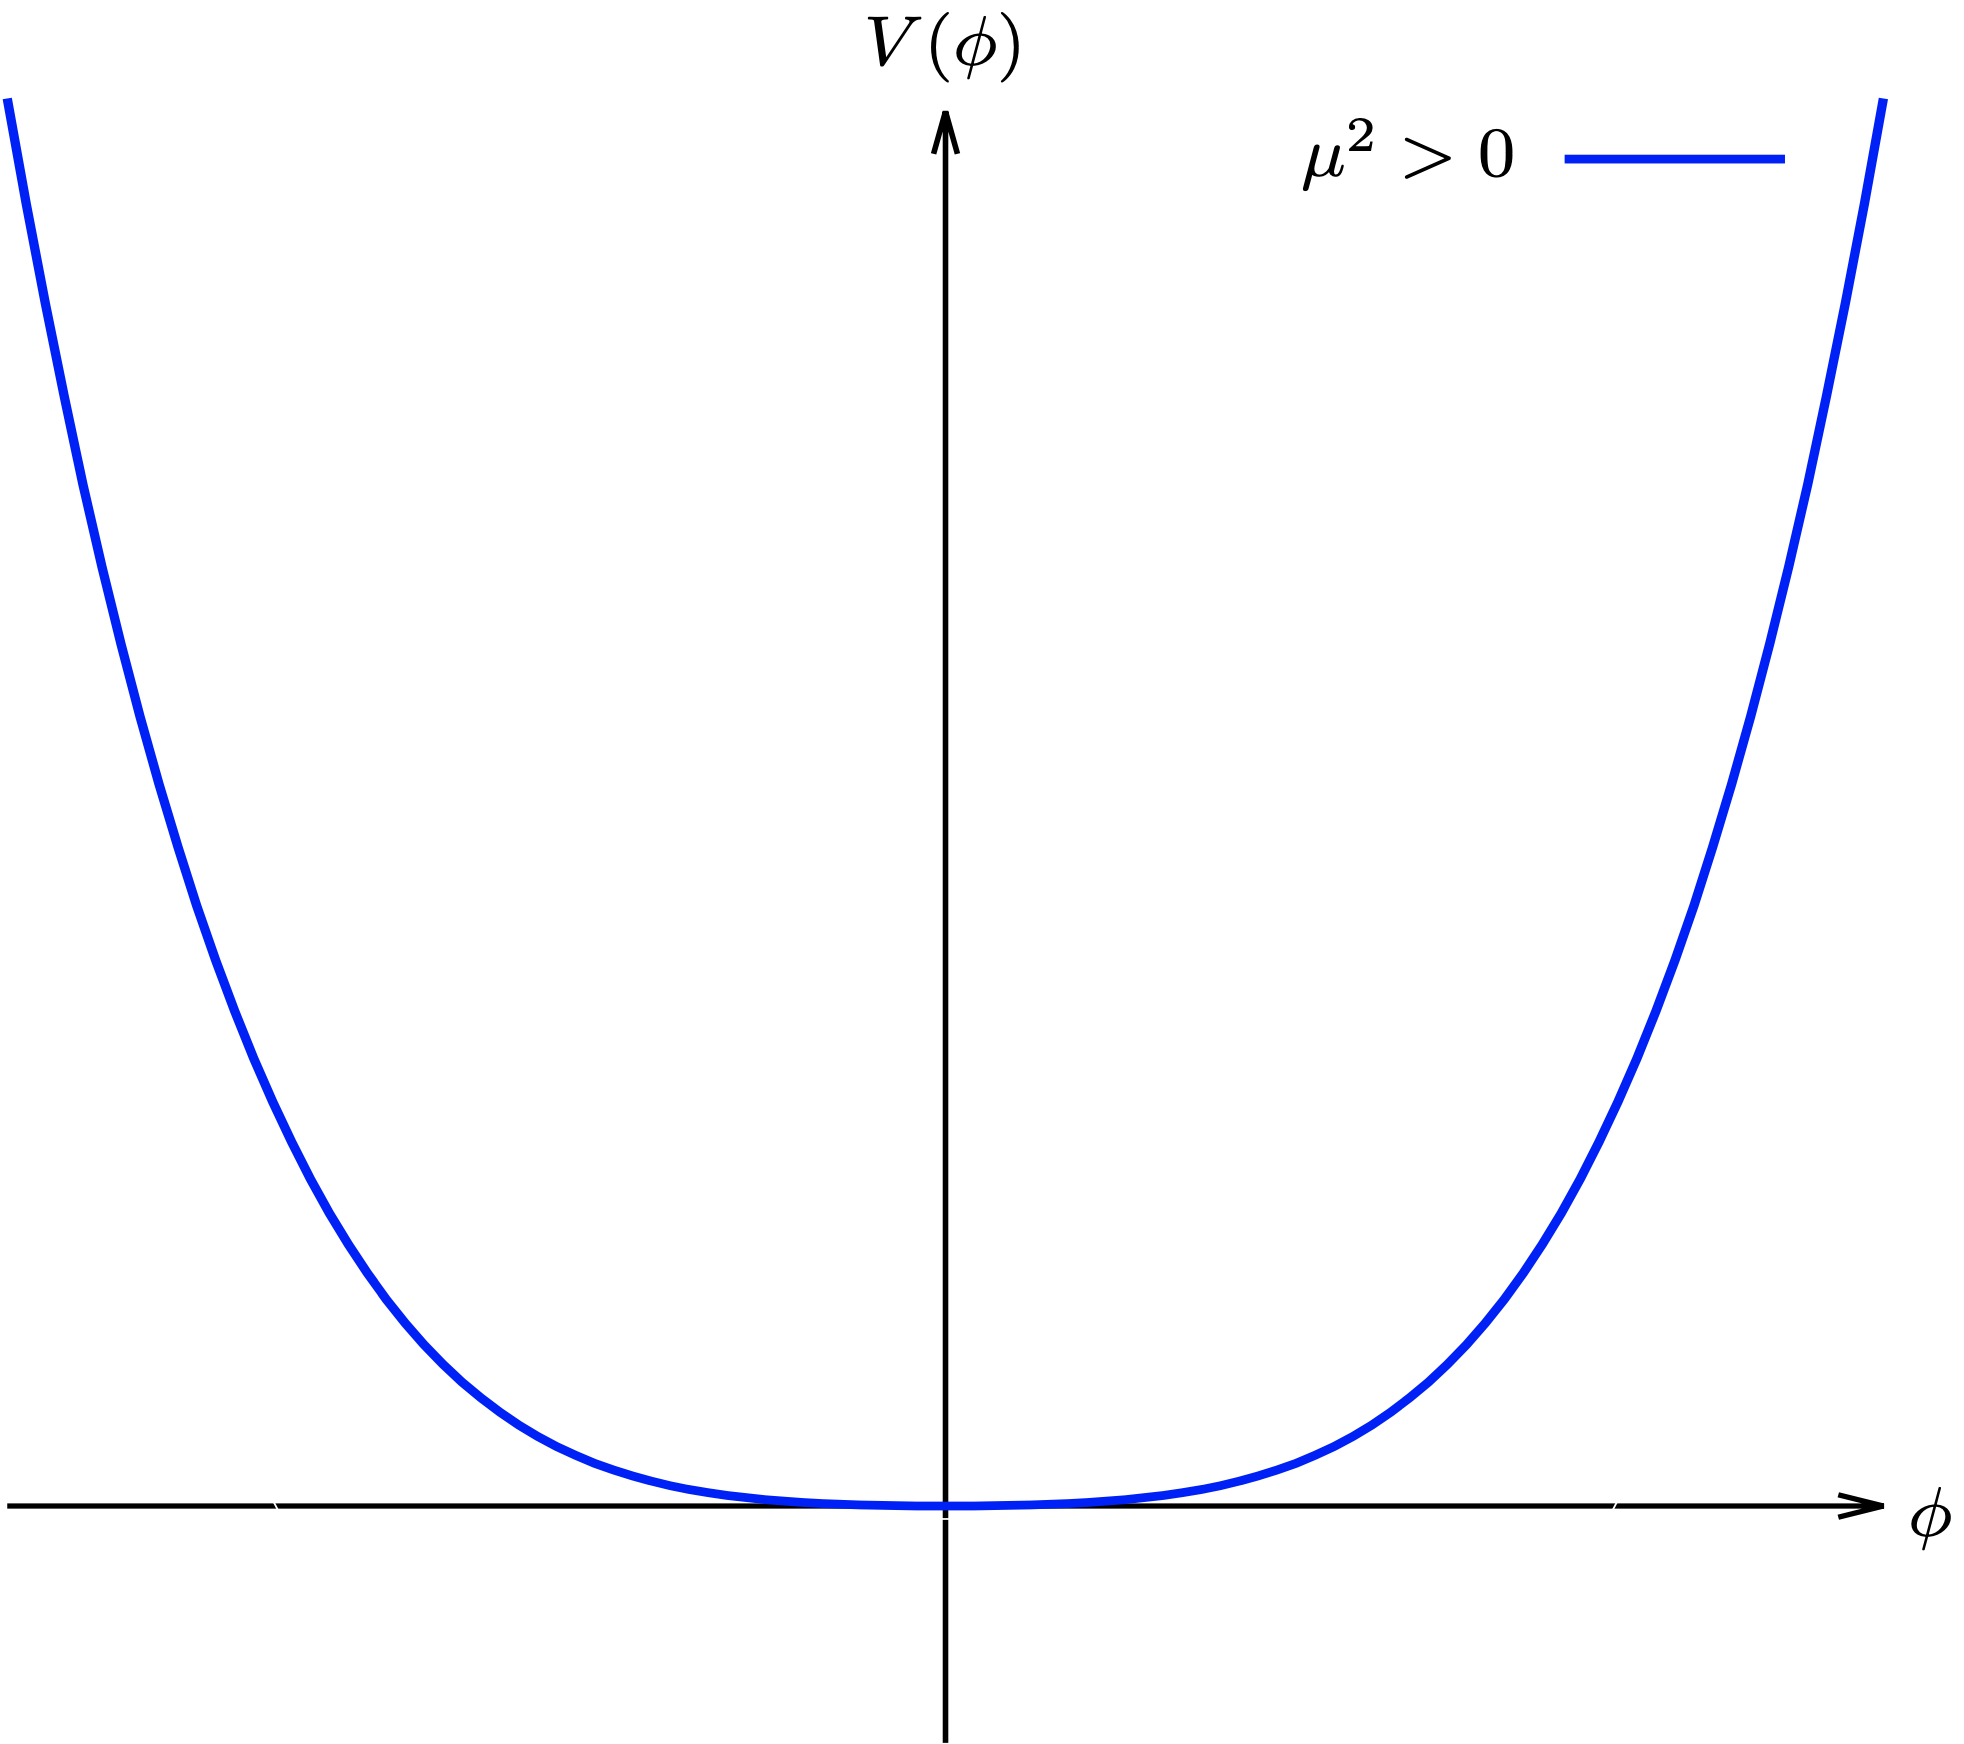
\includegraphics[width=.74\linewidth]{Chapter1/Higgs_V_muplus}
%  \caption{}
%  \label{fig:Chap1:SM:HiggsMechanism:PotentialExample:Positive}
%\end{subfigure}%
%\begin{subfigure}{.5\textwidth}
%  \centering
%  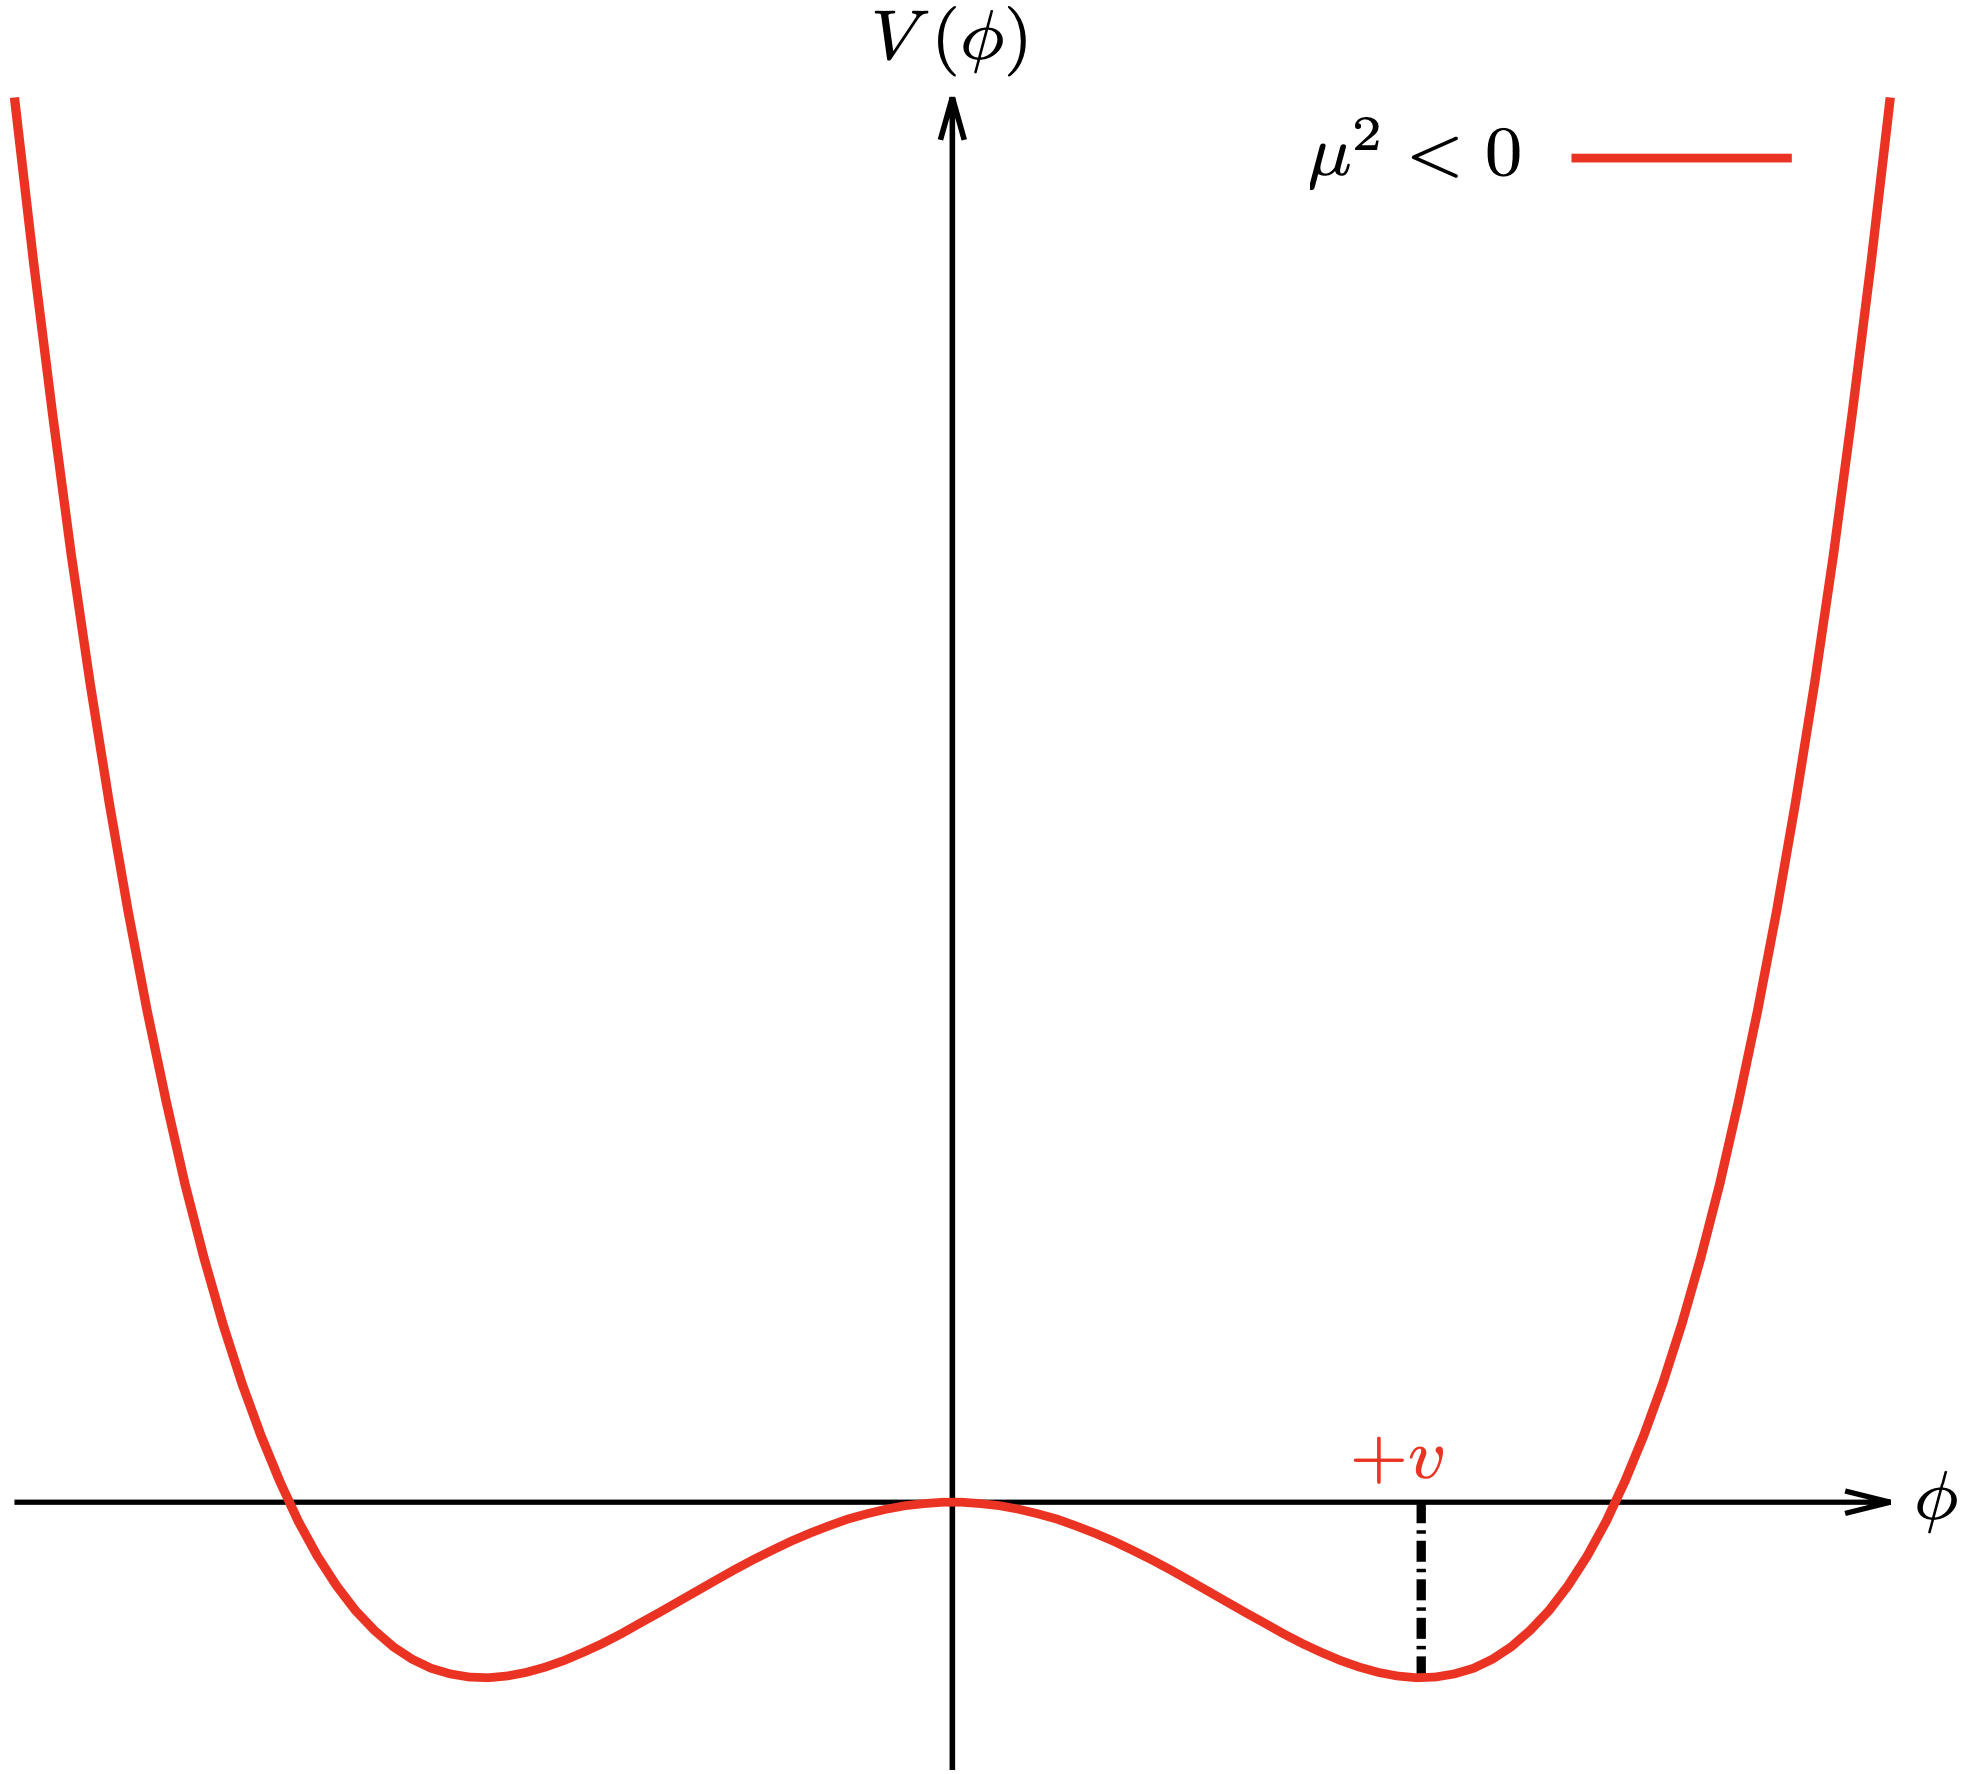
\includegraphics[width=.74\linewidth]{Chapter1/Higgs_V_muminus}
%  \caption{}
%  \label{fig:Chap1:SM:HiggsMechanism:PotentialExample:Negative}
%\end{subfigure}
%\caption{The potential $V(\phi)$ of Lagrangian \ref{eq:chap1:HiggsMechanism:Example} for(a) $\mu^{2}$ positive and (b) negative.}  
%\label{fig:Chap1:SM:HiggsMechanism:PotentialExample}
%\end{figure}
%Expanding the field around the minima at $\phi_{i} =(0,0,0,v)$, the $\mathcal{L}$ becomes:
%\begin{equation}
%\begin{split}
%	\mathcal{L} 	&= \frac{1}{2}\partial_{\mu}\sigma\partial^{\mu}\sigma + \mu^{2}\sigma^{2} -\sqrt{\mu^{2}\lambda}\sigma^{3} -\frac{1}{4}\lambda^{4} \\
%				& + \frac{1}{2}\partial_{\mu}\pi_{i}\partial^{\mu}\pi_{i} -\frac{1}{4}\lambda (\pi_{i}\pi_{i})^{4} - \lambda v \pi_{i}\pi_{i}\sigma - \frac{1}{2}\pi_{i}\pi_{i}\sigma^{2} \, ,
%\end{split}
%\end{equation}
%where $i$ runs from 1 to 3. Here $\sigma = \phi_{4}-v$ and $\pi_{i} = \phi_{i}$ are new boson fields, being the latter massless and the former with a mass of $m_{\sigma}^2 = -2\mu^{2}$.
%The new terms break the original symmetry because the symmetry of the Lagrangian is not longer a symmetry of the vacuum, it has been spontaneously broken.
%One massive $\sigma$ boson and three massless $\pi_{i}$ bosons with a residual $O(3)$ symmetry have appeared. This is a consequence of the Goldstone theorem which states that 
%``for a continuous symmetry group $\mathcal{G}$ spontaneously broken down to a subgroup $\mathcal{H}$, the number of broken generators is equal to the number of massless scalars 
%that appear in the theory''~\cite{Goldstone:1962es}. Therefore, since the $O(N)$ group has $N(N-1)/2$ generators, the $O(N-1)$ has $(N-1)(N-2)/2$ and, hence, $N-1$ Goldstone bosons
%appear. The example shown is for $N=4$.


\paragraph{The Higgs mechanism in the SM for bosons}\mbox{}\\
The Goldstone theorem  states that 
``for a continuous symmetry group $\mathcal{G}$ spontaneously broken down to a subgroup $\mathcal{H}$, the number of broken generators is equal to the number of massless scalars  that appear in the theory''~\cite{Goldstone:1962es}.
To apply this mechanism to the SM, it is necessary to generate mass for the \PWplus, \PWminus and \PZ bosons while keeping the photon massless. 
%The Higgs mechanism is based on the general idea of spontaneous symmetry breaking, meaning that for a system the ground state is not equivalent to a
%fully symmetric state. Implying that the systems evolves from a ground state which is not invariant under its full symmetry group.
To do so, the EW symmetry group $SU(2)_\text{L} \times U(1)_\text{Y}$ has to be broken into a $U(1)$ subgroup describing electromagnetism. 
A gauge-invariant interaction that gives masses to fermions without mixing chiral components
is introduced by defining a $SU(2)$ isospin doublet of complex scalar field with hypercharge $\text{Y}=1$:
\begin{equation*}
	\Phi = \begin{pmatrix} \phi^+ \\ \phi_0 \end{pmatrix}\, .
\end{equation*}
Being $\phi^+$ positively charged and $\phi^0$ neutral. The Lagrangian $\mathcal{L}_{\text{Higgs}}$ has to be added to the $\mathcal{L}_{\text{EW}}$ in equation~\ref{eq:chap1:EW:FinalL}.
\begin{equation*}\label{eq:chap1:HiggsMechanism:HiggsLagrangianA}
	\mathcal{L}_{\text{Higgs}} = (D_{\mu} \Phi)^{\dagger}(D^{\mu} \Phi) - V(\Phi) \textrm{ where } V(\Phi) = \mu^{2}\Phi^{\dagger} \Phi + \lambda (\Phi^{\dagger} \Phi)^{2}\, ,
\end{equation*}
with $\lambda >0$ required for vacuum stability. When $\mu^{2}>0$, the minimum of the potential occurs when both fields ($\phi^+$ and $\phi^0$) are at zero. If $\mu^{2}<0$, the 
minimum of the potential has an infinite number of degenerate states that satisfy $\Phi^{\dagger} \Phi = \mu^{2}/2\lambda$ and the physical vacuum state will correspond 
to any particular point on the circle of Figure~\ref{fig:Chap1:SM:HiggsMechanism:Potential}.
Having to choose a particular point breaks the global $U(1)$ symmetry of the Lagrangian. Without loss of generality, in this scenario, the ground state $\Phi_{0}$ can be chosen to be:
\begin{equation*}
	\Phi_{0} = \frac{1}{\sqrt{2}}\begin{pmatrix} 0 \\ v \end{pmatrix} \textrm{ where } v = 2\sqrt{\frac{\mu^{2}}{\lambda}}\, .
\end{equation*}
being $v$ the vacuum expectation value. This defines the already mentioned circle in the minimum of $V(\Phi)$ in the $\mu^{2}<0$ scenario.

\begin{figure}
    \centering
    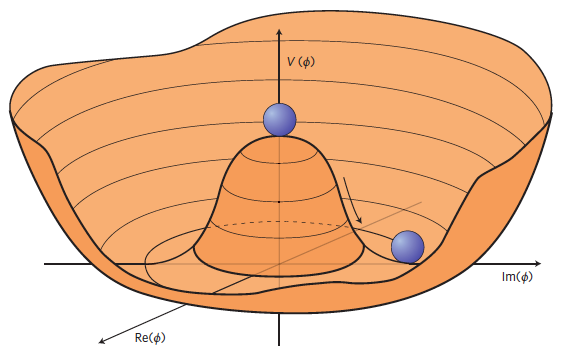
\includegraphics[width = 0.7\textwidth]{Chapter1/HiggsPotential}
    \caption{An illustration of the Higgs potential $V(\Phi)$ in the case of $\mu^{2}<0$~\cite{Bass:2764481}. Choosing any particular point in the circle defined by $v$ spontaneously breaks the $U(1)$ rotational symmetry. This type of potential is
    frequently called ``Mexican hat''.}
    \label{fig:Chap1:SM:HiggsMechanism:Potential}
\end{figure}

The Lagrangian density must be formulated in terms of deviations from one of these
ground states. This can be done by introducing an excitation, $h(x)$, that can be understood
as a small deviation of the field from the ground state. 
Accordingly, the fields can be expanded around the minimum as:
%\begin{equation*}
%	\Phi = \frac{1}{\sqrt{2}} \begin{pmatrix} 0 \\ v+h(x) \end{pmatrix} exp\{  i \chi(x)\}\, .
%\end{equation*}
%The new field $\chi(x)$ can be set to zero in the so called ``unitary gauge''.
\begin{equation}\label{eq:chap1:HiggsMechanism:SymmetryBreaking}
	\Phi = \frac{1}{\sqrt{2}} \begin{pmatrix} 0 \\ v+h(x) \end{pmatrix} \, ,
\end{equation}
%Expanding the covariant derivative of the $\mathcal{L}_{\text{Higgs}}$:
%\begin{equation*}\label{eq:chap1:HiggsMechanism:Covariant}
%\begin{split}
%	 (D_{\mu} \Phi)^{\dagger}(D^{\mu} \Phi) 	&=\left\lvert \left( \partial_{\mu} + ig \frac{\tau^{k}}{2} \PW_{\mu}^{k} (x)+ ig' \frac{y}{2} B_{\mu} \right)\right\rvert^{2} \\
%									&= \frac{1}{2} \left\lvert \begin{pmatrix}  \partial_{\mu} +i\frac{1}{2}(gW^{3}_{\mu}+g'\frac{y}{2} B_{\mu}) && i\frac{g}{2}(W^{1}_{\mu}-iW^{2}_{\mu}) \\
%									i\frac{g}{2}(W^{1}_{\mu}-iW^{2}_{\mu}) && \partial_{\mu} -i\frac{1}{2}(gW^{3}_{\mu}-g'\frac{y}{2} B_{\mu})
%									 \end{pmatrix}  \begin{pmatrix} 0 \\ v+h \end{pmatrix}\right\rvert ^{2} \\
%									 &= \frac{1}{2}(\partial_{\mu} h)^{2} + \frac{1}{8}(v+h)^{2}|W^{1}_{\mu}-iW^{2}_{\mu}|^{2} \\
%									 &+ \frac{1}{8}(v+h)^{2}|gW^{3}_{\mu}-g'B_{\mu}| +(\textrm{interaction terms}) \, ,
%\end{split}
%\end{equation*} %source: https://arxiv.org/pdf/1709.10508.pdf
%where the $\tau_k$ with $k={1,2,3}$ are the Pauli Matrices. In this equation there are terms mixing the $W^{3}$ and the $B_{\mu}$ fields that, by using the physical fields defined in equation~\ref{eq:chap1:EW:ZmuAmu}, should disappear since the physical bosons do not mix. Applying the Relation \ref{eq:chap1:EW:ZmuAmu} into the covariant derivative, 
and the covariant derivative takes the form:
\begin{equation*}
	(D_{\mu} \Phi)^{\dagger}(D^{\mu} \Phi) = \frac{1}{2}+\frac{g^2v^2}{4}W^{+}_{\mu} W^{-\, \mu} + \frac{g^{2} v^{2}}{8 \textrm{cos}^{2}\theta_{W}}Z_{\mu}Z^{\mu} \, , %+ 0 A_{\mu}A^{\mu}
\end{equation*}
where $\theta_{W}$ is the weak mixing angle, which is measured to be 
\mbox{$\textrm{sin}^{2} \theta_{W} = 0.2310\pm0.0005$}~\cite{CMS:2018ktx}.
By doing this, the \PWplus, \PWminus and \PZ bosons have finally acquired mass. Through the Higgs mechanism, their masses within the SM are:
\begin{align*}
	M_{\PW} = \frac{1}{2}gv 	&&  	\text{and}	&& M_{\PZ} = \frac{1}{2}\frac{gv}{\textrm{cos}\,\theta_{W}}\, .
\end{align*}
Additionally, a new scalar field $h(x)$ has appeared with its correspondent mass term, the Higgs field. Note that the $h(x)$ was introduced as a perturbation from the ground
state of the Higgs potential $V(\Phi)$, so the Higgs boson can be understood as an excitation of the Higgs potential. Apart from couplings to the electroweak gauge
fields, the Higgs field also has self-interaction vertices. The mass of this boson is $m_{\PHiggs}=\sqrt{2}\mu$.

With this covariant term, the Higgs Lagrangian density of the system is obtained:
%\begin{equation*}\label{eq:chap1:HiggsMechanism:HiggsLagrangianB}
%\begin{split}
%	\mathcal{L}_{\text{Higgs}} 	&= \frac{1}{2} (\partial_{\mu}h) (\partial^{\mu}h) + \frac{g}{4}(v+h)^{4}\PW_{\mu}\PW^{\mu} + \frac{g^{2}}{8 \textrm{cos}^{2}\theta_{W}}(v+h)^{2}\PZ_{\mu}\PZ^{\mu} \\
%					&+\frac{\mu^{2}}{2}(v+h)^{2} - \frac{\lambda}{16}(v+h)^{4}
%\end{split}
%\end{equation*}
%and expressing it in terms of the boson masses and coupling parameters, it can be written as:
\begin{equation}\label{eq:chap1:HiggsMechanism:HiggsLagrangianC}
\begin{split}
	\mathcal{L}_{\text{Higgs}} 	&= \frac{1}{2} (\partial_{\mu}h) (\partial^{\mu}h)  - \frac{1}{2}m^{2}_{\PHiggs}h^{2}+\frac{1}{2}m_{\PW}\PW_{\mu}\PW^{\mu}+\frac{1}{2}m_{\PZ}\PZ_{\mu}\PZ^{\mu} + g m_{\PW} h \PW_{\mu}\PW^{\mu} \\
					&+ \frac{g^{2}}{4}\PW_{\mu}\PW^{\mu} + g \frac{m_{\PZ}}{2 \textrm{cos}\,\theta_{W}} h \PZ_{\mu}\PZ^{\mu} - g^{2}\frac{1}{4 \textrm{cos}^{2}\theta_{W}}h^{2}\PZ_{\mu}\PZ^{\mu} 
					 -g \frac{m^{2}_{H}}{4 m_{\PW}}h^{3} \\
					& -g^{2}\frac{m^{2}_{H}}{32 m^{2}_{\PW}}h^{4}+\textrm{const.}
\end{split}
\end{equation}
As can be seen in the Lagrangian in equation~\ref{eq:chap1:HiggsMechanism:HiggsLagrangianC}, the coupling strengths of the \PW and \PZ 
fields to the Higgs field are proportional to $m_{\PW}$ and $m_{\PZ}$, respectively.
%This why it is said that the more a fundamental particle interacts with the Higgs boson, the more massive it is.
% It is not that the particles that have more mass interact more with the Higgs fields but the 
% other way round: the particles that interact more with the Higgs fields have more mass, i.e. the interaction with the Higgs proceeds the mass of the particles.

%Another way to interpret this is by understanding the mass as the tendency to resist movement, therefore, if a particle interacts strongly with the Higgs field, it is more difficult for that particle to 
%move and hence this particle is more massive. The Higgs field acts as a viscosity. 

\paragraph{The Higgs mechanism in the SM for fermions}\mbox{}\\ %Source: Book - Modern Particle Physics - Mark Thompson (me lo prestó Stef)
The Higgs mechanism for spontaneous symmetry breaking of the $SU(2)_\text{L} \times U(1)_\text{Y}$ gauge group of the SM generates the masses of the \PWpm and \PZ bosons.
For originating the mass of the fermions without violating the EW gauge symmetry a similar procedure is carried but taking into account that the left-handed particles transform differently 
than the right-handed. To do so, additional terms including the Yukawa couplings are added into the Lagrangian. These terms are of the form:
\begin{align*}
\mathcal{L}_{\text{Yukawa,} f}=-y_{f}(\bar{\chi}_{L}^f \Phi \chi_\text{R}^{f} + \bar{\chi}_{\text{R}}^f \Phi^{\dagger} \chi_\text{L}^{f} )\, \text{, with }\, \Phi = \begin{pmatrix} \phi^+ \\ \phi_0 \end{pmatrix} 
\end{align*}
where the $f$ superindex runs over all quarks and charged leptons. %It is usual to express the second part of the sum just as ``plus hermitic conjugate'' (``+ h.c.''). Note that the hermitic conjugate part
%is necessary to ensure that expression fulfils the requirement for a hermitian operator to be self-adjoint in a complex Hilbert space.
The different $y_f$ constants are known as Yukawa couplings of the particle $f$ to the Higgs field. The Higgs doublet is denoted by $\Phi$.
For the electron $SU(2)$ doublet, the element with this coupling can be written as:
\begin{equation}\label{eq:chap1:HiggsMechanism:ElectronDoubletLagrangian}
\mathcal{L}_{\Pe} = - y_{\Pe} \left[ (\bar{\Pnu}_{\Pe} \bar{\Pe})_{\text{L}} \begin{pmatrix} \phi^{+} \\ \phi^{0} \end{pmatrix} \Pe_{\text{R}} + \bar{\Pe_{\text{L}}} (\phi^{+*} \phi^{0*})\begin{pmatrix} \Pnu_{\Pe} \\ \Pe \end{pmatrix}_{\text{L}} \right] \, .
\end{equation}
Here, $y_{e}$ is the Yukawa coupling of the electron to the Higgs boson. 
After spontaneously breaking the symmetry as it is done 
in equation~\ref{eq:chap1:HiggsMechanism:SymmetryBreaking}, and the 
$y_{\Pe}$ is set to $y_{\Pe}=\sqrt{2}\,m_{\Pe}/v$ where $m_{\Pe}$ is the observed 
electron mass, 
 the Lagrangian in equation~\ref{eq:chap1:HiggsMechanism:ElectronDoubletLagrangian} becomes:
%\begin{equation}\label{eq:chap1:HiggsMechanism:ElectronBroken}
%\mathcal{L}_{\Pe} = \frac{-y_{\Pe}}{\sqrt{2}} v (\bar{\Pe}_{\text{L}}\Pe_{\text{L}} + \bar{\Pe}_{\text{L}}\Pe_{\text{L}}) + \frac{-y_{\Pe}}{\sqrt{2}} h (\bar{\Pe}_{\text{L}}\Pe_{\text{L}} + \bar{\Pe}_{\text{L}}\Pe_{\text{L}} )
%\end{equation}
%The $y_{\Pe}$ is not predicted by the Higgs mechanism, but can be chosen to be consistent with the observed electron mass ($m_{\Pe}$) so that $y_{\Pe}=\sqrt{2}\,m_{\Pe}/v$. Using this relation, the Lagrangian in \ref{eq:chap1:HiggsMechanism:ElectronBroken} becomes:
\begin{equation}\label{eq:chap1:HiggsMechanism:ElectronMassL}
\mathcal{L}_{\Pe} = -m_{\Pe} \bar{\Pe}\Pe - \frac{m_{\Pe}}{v}\bar{\Pe}\Pe h
\end{equation}
The first element of the Lagrangian in equation~\ref{eq:chap1:HiggsMechanism:ElectronMassL} gives mass to the electron and gives rise to the coupling of the electron to the Higgs fields in its non-zero vacuum expectation. 
The second term represents the coupling of the electron and the Higgs boson itself.

The non-zero vacuum expectation value occurs only in the neutral part of the Higgs doublet due to the form 
in the ground state in equation~\ref{eq:chap1:HiggsMechanism:SymmetryBreaking}. This implies that the combination $\bar{\chi}_{\text{L}}^f \Phi \chi_\text{R}^{f} + \bar{\chi}_{\text{L}}^f \Phi^{\dagger} \chi_\text{L}^{f}$ can only generate
masses for the fermions in the lower component of an $SU(2)$ doublet, i.e. the charged leptons and the down type quarks. Putting aside the procedure to give mass to the up-type quarks,
this explains why the neutrinos do not get mass through the Higgs mechanism.

%For the up-type quarks, a gauge invariant term can be constructed from $\bar{\chi}_{\text{L}}^f \Phi_{c} \chi_\text{R}^{f} + \bar{\chi}_{\text{L}}^f \Phi_{c}^{\dagger} \chi_\text{L}^{f}$:
%\begin{equation*}%\label{eq:chap1:HiggsMechanism:UpType}
%\mathcal{L}_{\Pup} = y_{\Pup} (\bar{\Pup} \bar{\Pdown})_{\text{L}} \begin{pmatrix} -\phi^{0*} \\ \phi^{-} \end{pmatrix} \Pup_{\text{L}} + \textrm{h.c.}
%\end{equation*}

For up-type quarks, after applying the symmetry breaking and using $y_{\Pup}=\sqrt{2}\,m_{\Pup}/v$, the Lagrangian density takes the form:
%\begin{equation*}\label{eq:chap1:HiggsMechanism:UpTypeBroken}
%\mathcal{L}_{\Pup} = \frac{-y_{\Pup}}{\sqrt{2}} v (\bar{\Pup}_{\text{L}}\Pup_{\text{L}} + \bar{\Pup}_{\text{L}}\Pup_{\text{L}}) + \frac{-y_{\Pup}}{\sqrt{2}} h (\bar{\Pup}_{\text{L}}\Pup_{\text{L}} + \bar{\Pup}_{\text{L}}%\Pup_{\text{L}} )
%\end{equation*}
%with a Yukawa coupling between the up quark and the boson $y_{\Pup}=\sqrt{2}\,m_{\Pup}/v$, resulting in:
\begin{equation*}%\label{eq:chap1:HiggsMechanism:ElectronMassL}
\mathcal{L}_{\Pup} = -m_{\Pup} \bar{\Pup}\Pup - \frac{m_{\Pup}}{v}\bar{\Pup}\Pup h .
\end{equation*}

%Therefore, for Dirac fermions, mass terms that let the Lagrangian invariant under local gauge transformations can be constructed from
%\begin{align*}%\label{eq:chap1:HiggsMechanism:ForFermions}
%\mathcal{L} = -y_{f}\left[\bar{\chi}_{\text{L}}^f \Phi \chi_\text{R}^{f} + (\bar{\chi}_{\text{L}}^f \Phi \chi_\text{L}^{f} )^{\dagger} \right] && \textrm{ or } && \mathcal{L} = y_{f}\left[\bar{\chi}_{\text{L}}^f \Phi_{c}\chi_\text{R}^{f} + (\bar{\chi}_{\text{L}}^f \Phi_{c} \chi_\text{L}^{f} )^{\dagger}\right] .
%\end{align*}
%The left Lagrangian is used for the leptons and down-type quarks, while the right one is used for the up-tupe quarks. 
These elements give rise not only to the mass of the fermions but also to the interaction
strengths between these fermions and the Higgs boson. The Yukawa coupling of the fermions to the Higgs field is given by:
\begin{equation}\label{eq:chap1:HiggsMechanism:YukawaCoupling}
	y_{f} = \sqrt{2} \, \frac{m_{f}}{v} \, ,
\end{equation}
where the Higgs vacuum expectation value is fixed by the Fermi coupling $G_{F}$ and is measured to be $v = \sqrt{2}\,G_{F} \approx 246.22$~GeV. The $G_{F}$ 
is measured from the antimuon ($\APmuon$) lifetime measurement~\cite{MuLan:2010shf}. 
%The $G_{F}$ is also used to determine the magnitude of the elements in the CKM matrix.

The value of fermionic masses is not predicted by the SM but obtained through experimental observations.
Given the measured top-quark mass, $\mtop = 172.76 \pm 0.30$~GeV~\cite{Workman:2022ynf}, it is of particular interest the Yukawa coupling of the top quark to the Higgs field (\yt), which is almost exactly equal to one. %~\cite{pdgTop}
 It is important to verify this because deviation of the measured \yt from the SM prediction would be proof of new physics.
 The object of this thesis is precisely the measurement of a process whose cross-section is directly related to \yt.
 %phenomena beyond the SM that could provide an 
%answer to several open questions concerning the fundamental interactions of elementary particles.
%For the top quark, the Yukawa coupling, $y_t$ almos exactly the unity. 


%https://www.youtube.com/watch?v=2TYFNOArnYo&t=2006s 






%%%%%%%%%%%%%%%%%%%%%
%                  Charge Parity                    %
%%%%%%%%%%%%%%%%%%%%%
%\subsection{Charge-Parity}
%\label{sec:chap1:CP_Violation}
% https://www.damtp.cam.ac.uk/user/tong/qft/four.pdf   <- p. 93-95 or PT and 96-96 C
% Parity and Charge conjugation: https://ocw.mit.edu/courses/physics/8-323-relativistic-quantum-field-theory-i-spring-2008/lecture-notes/ft1ls06p_08.pdf
% Intro of this paper: https://arxiv.org/pdf/2201.02385.pdf
% ATLAS: https://atlas.cern/updates/briefing/symmetry-breaking-higgs-boson <- Searching for new sources of matter–antimatter symmetry breaking in Higgs boson interaction with top quarks

%\pablo{Probably, this section is gonna be absorbed by \ref{sec:chap1:EW}}


%%%%%%%%%%%%%%%%%%%%%
%                        Wrap up                        %
%%%%%%%%%%%%%%%%%%%%%
\section{Remarks about the limitations of the Standard Model}
\label{sec:chap1:Wrapup}
%Once the gauge symmetries and the fields with their gauge quantum numbers are specified, the Lagrangian of
%the SM is fixed by requiring it to be invariant under local gauge transformations, and renormalisable. 
%The SM Lagrangian can be divided into several pieces.

%Perhaps the ultimate and definitive (if talking about definitive makes any sense) theory of particle physics 
%is a simple equation with a small number of free parameters. Meanwhile, the SM is here, and while it is not
But the SM is not  
the ultimate theory, it is unquestionably one of the greatest successes of modern physics.
Despite its achievements, many questions remain unsolved.


\subsection{The parameters of the Standard Model}
\label{sec:chap1:Wrapup:ParamsOfSM}
The SM contains 25 free parameters that must be determined through experimentation. 
These are the masses of the 12 fermions, %(assuming colour variations and antiparticles that are not viewed as 
%separate fermions) or, more precisely, the 12 Yukawa couplings to the Higgs field, % ($m_{\nu_{1}}, m_{\nu_{2}}, m_{\nu_{3}}, m_{e}, m_{\mu}, m_{\tau},
%	m_{u}, m_{d}, m_{c}, m_{s}, m_{t} \textrm{ and }  m_{b}$)
%	
%\begin{equation*}
%	m_{\nu_{1}}, m_{\nu_{2}}, m_{\nu_{3}}, m_{e}, m_{\mu}, m_{\tau},
%	m_{u}, m_{d}, m_{c}, m_{s}, m_{t} \textrm{ and }  m_{b}
%\end{equation*} 
the three coupling constants for describing the strength of the gauge interactions ($g, g' \textrm{ and } g_{s}$)
%\begin{equation*}
%	g, g' \textrm{ and } g_{s}
%\end{equation*} 
 and the two parameters describing the Higgs potential ($\mu$ and $\lambda$) or, equivalently, its vacuum  
expectation value $v$, and the Higgs-boson mass $m_{h}$.
%\begin{equation*}
%	v \textrm{ and }m_{h}
%\end{equation*} 
Finally, there are three mixing angles and the complex phase of the CKM matrix and four 
Pontecorvo--Maki--Nakagawa--Sakata matrices, %($\theta_{12}, \theta_{13}, \theta_{23}, \rho_{13}, \theta'_{a}, \theta'_{b}, \theta'_{c} \textrm{ and }\theta'_{d}$)
which mix the neutrino-mass eigenstates with neutrino-flavour eigenstates~\cite{Maki:1962lba, Pontecorvo:1957qd}.
%\begin{equation*}
%	\theta_{12}, \theta_{13}, \theta_{23}, \rho_{13}, \theta'_{a}, \theta'_{b}, \theta'_{c} \textrm{ and }\theta'_{d}
%\end{equation*} 

From the 25 free parameters of the SM, 14 are associated with the Higgs field, eight with the flavour sector and
only three with the gauge interactions. This emphasises the crucial significance of precisely measuring and 
comprehending the properties of the Higgs particle.

%%%%%%%%%%%%%%%%%%%%%%%%
%                  Problems with the SM                  %
%%%%%%%%%%%%%%%%%%%%%%%%
\subsection{Limitations of the Standard Model}
\label{sec:chap1:SM_problems}
While the SM is an extremely successful theory that has passed rigorous testing %, this is not the end of the story, since
there are several limitations of the SM and a variety of phenomena that it does not explain. %The SM 
%does not explain all questions in the universe and, hence, physicists continue looking for more general theories 
%to better explain the universe.  There is a long list of issues with the SM but, 
In the following pages, the most relevant issues with the SM are described.

\paragraph{Matter--antimatter asymmetry}\mbox{}\\
In principle, the Big Bang should have produced an equal amount of matter and antimatter 
which would all have then annihilated, leaving behind an empty universe filled with electromagnetic radiation.
 However, everything that is observed nowadays constituted of matter, from the tiniest life forms 
 on Earth to the greatest celestial objects. In comparison, there is not a lot of antimatter around. 

By looking at the cosmic microwave background (CMB) radiation, which contains the residual \Pgamma of the Big Bang, researchers 
have determined that there was a symmetry between the matter and antimatter content in the early universe. 
For every $3 \times 10^{9}$ antimatter particles, there were $3 \times 10^{9}$ and 1 matter particle.
The matter and antimatter annihilated and produced the CMB and the remaining 1 part turned into all the 
stars and galaxies that are seen.  %The field of cosmology that studies the processes that produced an 
%asymmetry between leptons and antileptons in the very early universe is called leptogenesis.

Research carried out during the last few decades has revealed that the laws of nature do not equally apply to
matter and antimatter~\cite{Sakharov:1967dj}. So far, the only non-trivial difference between matter and 
antimatter found is the \CP asymmetry or \CP violation. 
However, the \CP asymmetry included in the SM and observed in the experiments is insufficient 
to explain the composition of the observable universe and, hence, extensive searches for new sources of \CP 
violation are being carried out.
In this context, the study in this thesis seeks for new \CP-violation sources. %As Section
%\ref{sec:Chap1:tHq} details, the observation of a cross-section 
% greater than the one predicted by the SM may imply
%that the associated production of a Higgs boson and a single top quark does not conserve \CP.


%Where is the antimatter? One could think about antimatter galaxies, in the end, matter and antimatter emit the same kind of radiation. But, since the 
%antimatter galaxy would be surrounded by anti-hydrogen halo, when the halo of a matter galaxy and the halo of an antimatter galaxy enter in contact,
%the electrons and positrons of the halo would annihilate each other producing gamma rays. This gamma rays have not been observed and, hence,
%the existence of antimatter galaxies is desecrated.




%\paragraph{Strong \CP problem}\mbox{}\\ %https://cds.cern.ch/record/2652742/files/CERN-THESIS-2018-297.pdf
%https://inspirehep.net/literature/2089044
%\pablo{Write some lines here}



\paragraph{Gravity}\mbox{}\\
Gravity is the first force that any person learns about and the one known by humankind for longer. 
The SM describes all fundamental interactions but gravity. %In Table~\ref{tab:Chap1:FundamentalInteractions},
%the four forces are presented along with the theories to describe them. 
%While QCD, QED and EW interactions are part of the SM, the GR is not. 
GR is a geometric theory that currently describes gravitation in modern physics.
Some of the suggested solutions to integrate gravitational interactions in the SM consist of
postulating a new force carrier particle, the ``graviton'', that mediates this interaction in a similar way to how the gauge bosons
were proposed. Other explanations state that gravity can only be described by a deeper theory in which the 
time--space structure is not flat but dynamic. 

\paragraph{Neutrino masses}\mbox{}\\
According to the SM, the neutrinos are massless, nevertheless, many experiments confirm that this is not 
true~\cite{KATRIN:2021uub}. This is due to a property of neutrinos that allows them to change their flavour 
while travelling through space, this feature is known as ``neutrino oscillations''. Each of the three neutrino flavours
(\Pnue, \Pnum, \Pnut)
is a linear combination of three discrete neutrino-mass eigenstates ($\Pnu_{i}$ with $i\in\{1,2,3\}$) with mass eigenvalues 
($m_i$). While the neutrino oscillation experiments could probe the squared neutrino-mass eigenvalues 
($\Delta m^{2}_{ij}$), both the total scale of the masses and the sign of $\Delta m_{ij}$ remain as some of the most 
relevant open questions in particle physics. %Regarding to the sign of $\Delta m_{ij}$, it is known that the mass of 
%$\Pnu_{2}$ is slightly higher than $\Pnu_{1}$ ($\Delta m^{2}_{21}\equiv m^{2}_{2} - m^{2}_{1} \sim 10^{-4}$~eV) but 
%for the third mass eigenstate it has not been measured yet whether it is greater (normal ordering) or lower (inverted 
%ordering) than the other two, as it is depicted in Figure~\ref{fig:Chap1:Neutrino_problem}. Nevertheless, 
%the absolute square difference is known ($\Delta m^{2}_{31}\equiv |m^{2}_{3} - m^{2}_{1}| \sim 10^{-3}$~eV). 

%\begin{figure}
%    \centering
%    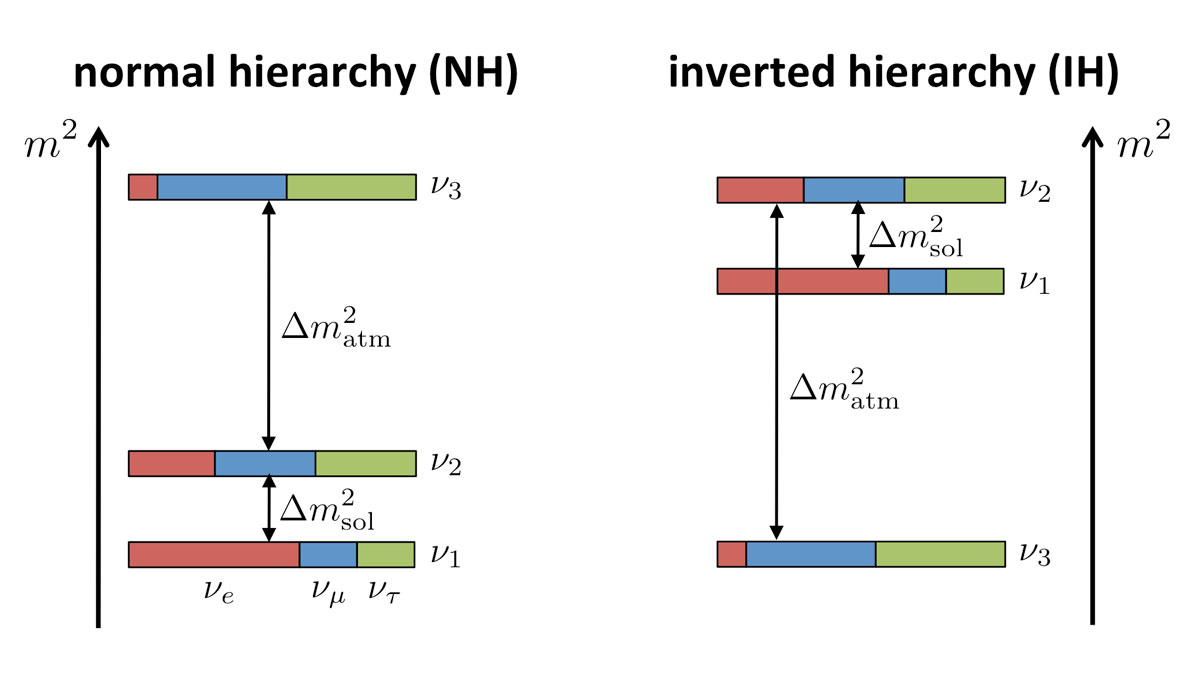
\includegraphics[width = 0.65\textwidth]{Chapter1/Neutrino_problem}
%    \caption{Two potential mass orderings of neutrinos are the normal ordering (normal hierarchy) and the inverted ordering (inverted hierarchy).}
%    \label{fig:Chap1:Neutrino_problem}
%\end{figure}

Non-zero neutrino masses opened an interesting portal beyond SM physics and, 
even though neutrinos are very elusive when it comes to detecting them, some 
next-generation experiments such as Dune~\cite{DUNE:2020lwj} target to set 
competitive and model-independent limits on neutrino masses. 

Regarding the nature of the neutrino mass, one could add mass terms to the SM as it is done in Section~\ref{sec:chap1:ParticleMasses:HiggsMechanism} 
for the up-type quarks but the origin of the neutrino masses is still not known. 
% It is possible that this mass comes from the Higgs mechanism, however, this is not clear.
Also, if neutrinos gained mass through Yukawa interaction, it would imply the presence of right-handed neutrinos, 
which has not been observed.

% Sterile neutrinos: special kind of neutrino that is proposed to explain some unexpected experimental results, but they have not been definitively discovered

% -  Neutrinos are the most elusive particles of the SM due to the difficulty of detect hem. However, some next generation experiments such 
% as Dune (Liquid argon detector) are very promising when it comes to set competitive and model independent limits on neutrino masses


\paragraph{Dark energy}\mbox{}\\
According to cosmological observations, the matter described by the SM only makes up around 5\% of the universe.
It turns out that roughly 68\% of the universe is made of dark energy, which is not considered by the SM.
%\begin{wrapfigure}{R}{0.5\textwidth}
%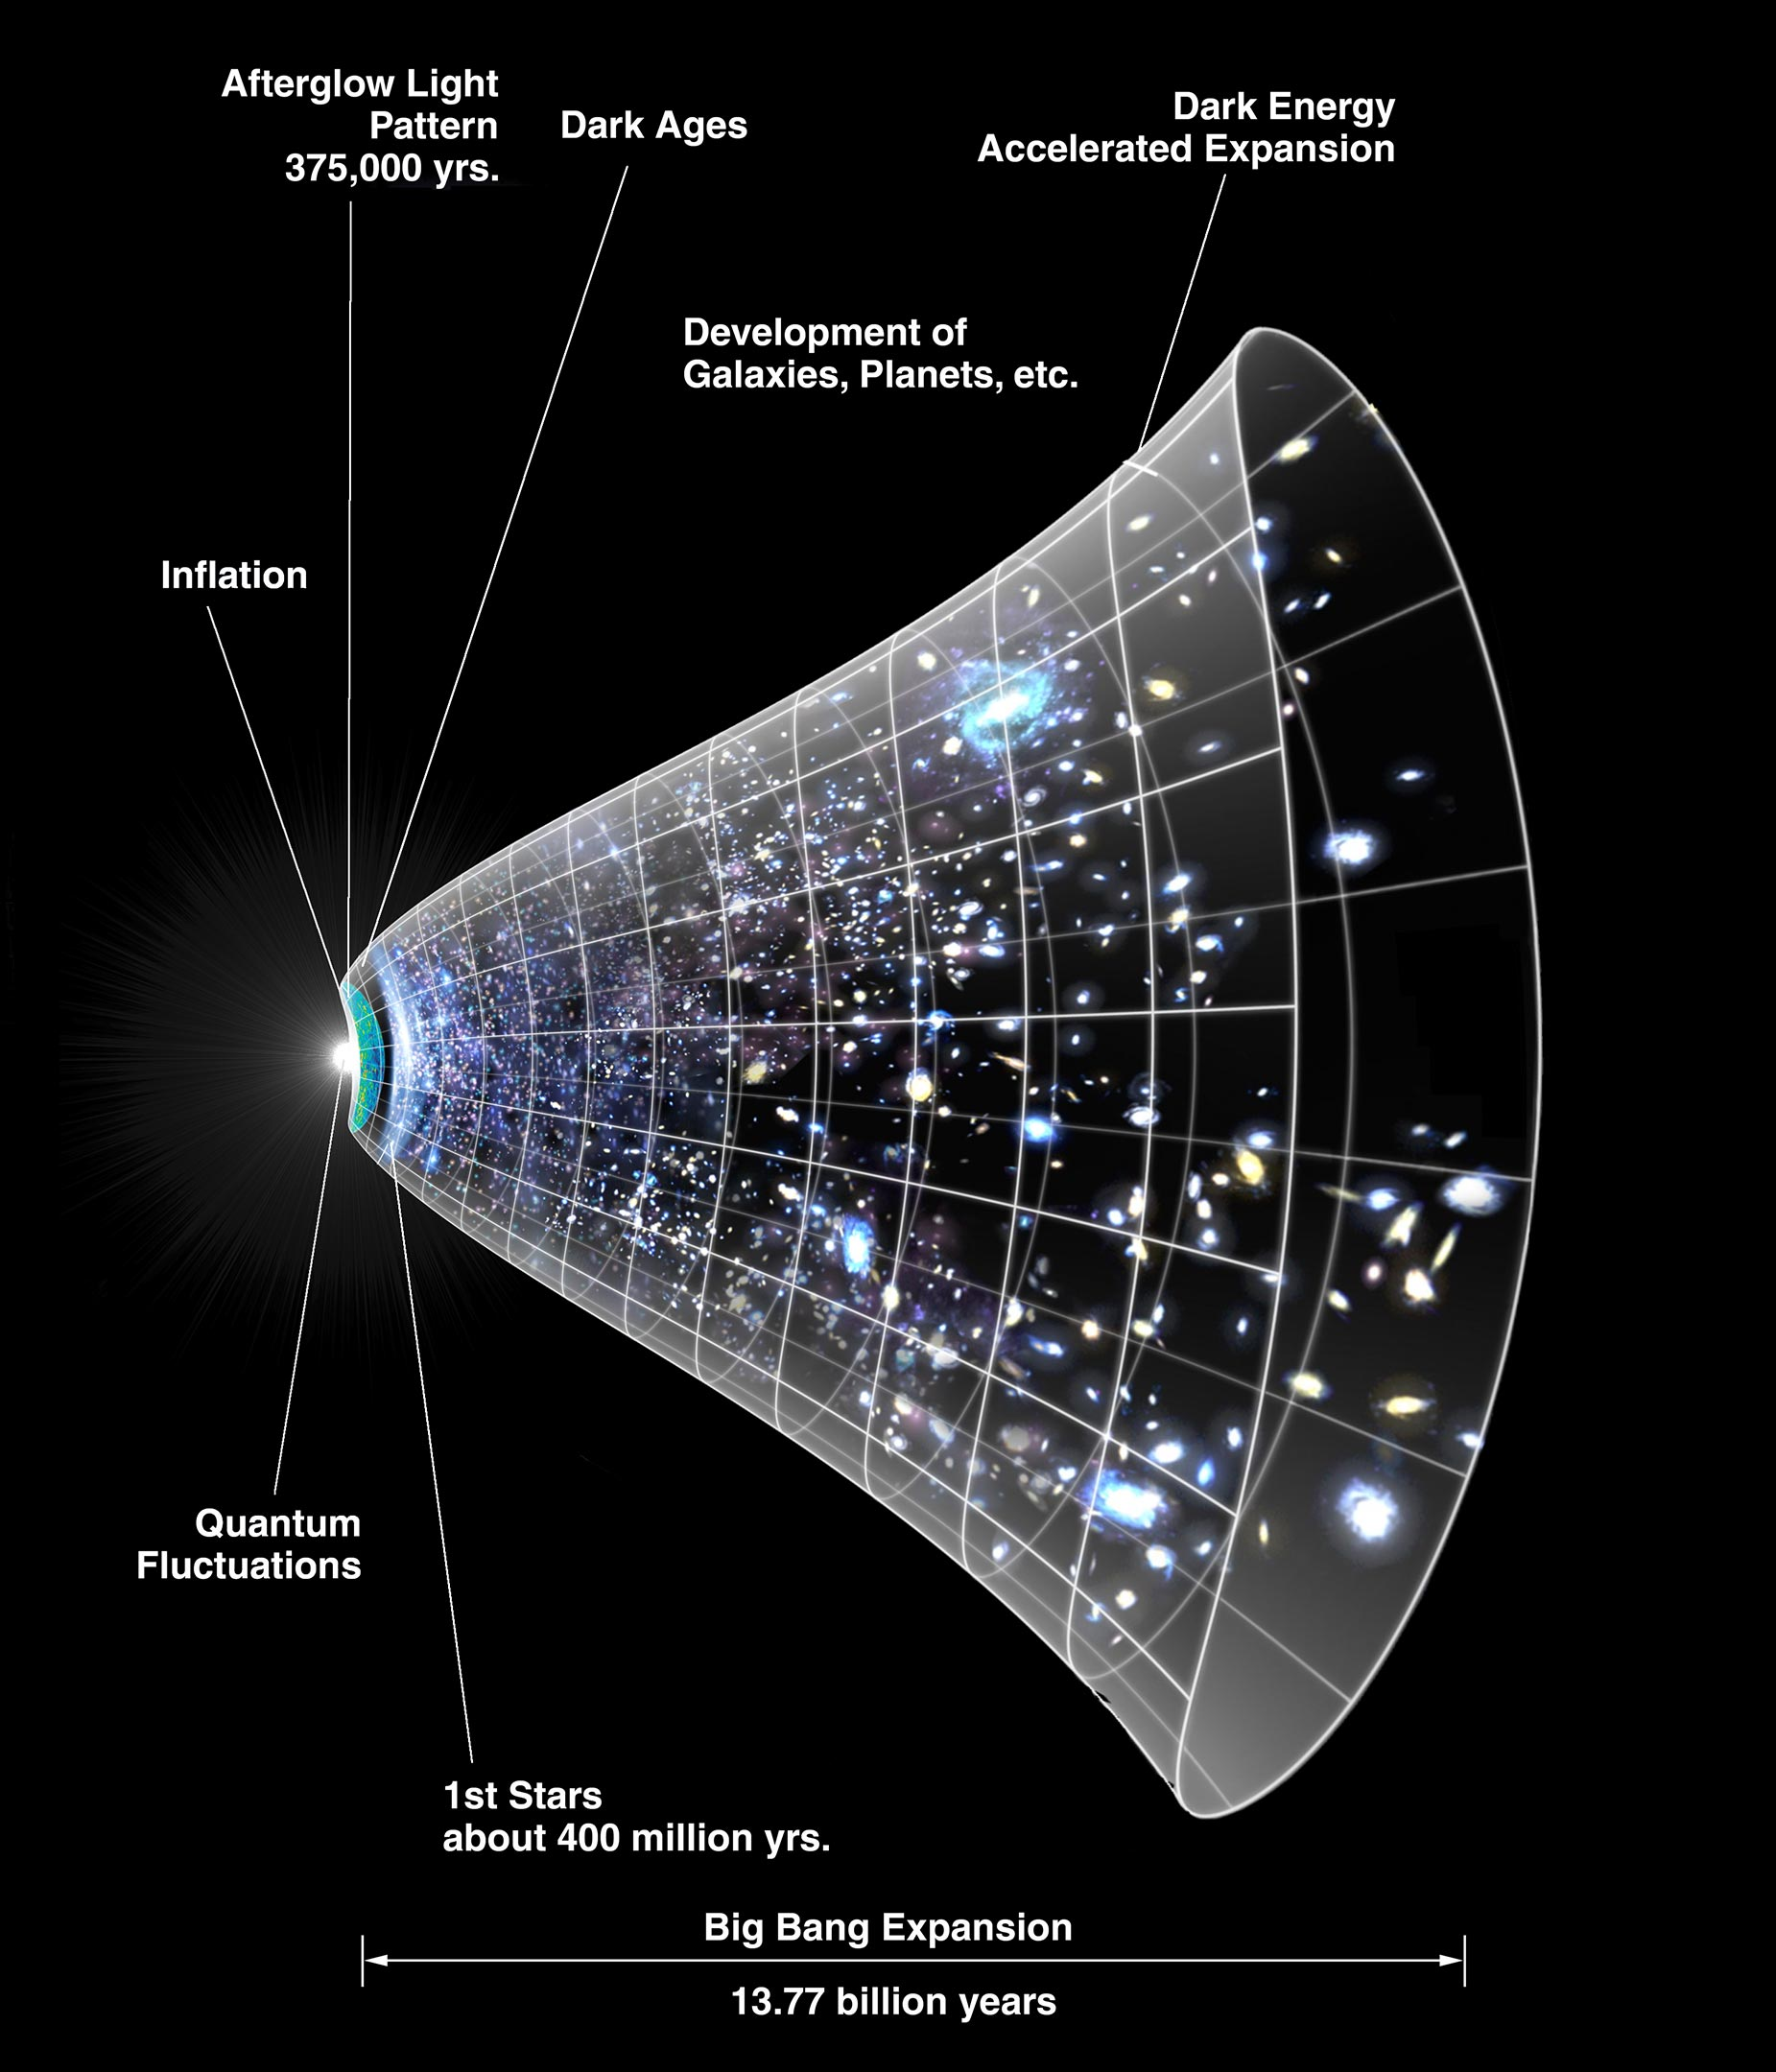
\includegraphics[width = 0.4\textwidth]{Chapter1/Limitations-UniverseExpansion}
%	\caption{The universe’s expansion over time. The dark-energy existence is suggested to explain this expansion.} %Credit: NASA/WMAP Science Team/ Art by Dana Berry
%	\label{fig:Chap1:UniverseExpansion}
%\end{wrapfigure} 

Dark energy is an unknown type of energy postulated to explain the observed accelerated expansion of the universe.
% as Figure~\ref{fig:Chap1:UniverseExpansion}.
This expansion is dominated by a spatially smooth component with negative pressure called dark energy.  
Modern cosmological measurements are based on supernovae, cosmic microwave background fluctuations,
galaxy clustering and weak gravitational lensing, and methods agree with a spatially flat universe with about 30\% matter (visible
and dark) and 70\% dark energy~\cite{Planck:2018vyg}.
%source:https://inspirehep.net/files/623a507c0d34d855e16642fb216668ab



\paragraph{Dark matter}\mbox{}\\
Dark matter (DM) adds up to approximately 85\% of all matter content in the universe. %and 27\% of all energy. 
This matter is called dark because it does not interact with the electromagnetic field. %, so maybe a name such us invisible matter would have been more appropriate
% since rather than being dark it just does not emit or reflect light.
The only known way to interact with DM is via gravitational interaction, which is about 25 orders of
magnitude weaker than the weak force (see Table~\ref{tab:Chap1:FundamentalInteractions}). This is why DM is so difficult to detect. 
The SM does not provide a proper explanation but searches are being carried and candidates such as 
weakly-interacting massive-particles (WIMPs) or axions\footnote{An axion is a hypothetical elementary particle postulated to resolve the strong \CP problem~\cite{Weinberg:1977ma, Wilczek:1977pj}.}.

The existence of DM is inferred through gravitational effects in astrophysical and cosmological observations. 
The rotational speed of the galaxies~\cite{Rubin:1970zza}, the gravitational lensing~\cite{Taylor:1998uk} and the CMB angular spectrum~\cite{Planck:2015fie} are
some examples of phenomena that cannot be explained with general relativity unless there is more present matter than what is seen.

Although the vast majority of the scientific community accepts dark matter existence, alternative explanations for the observed phenomena have suggested. 
Most of these model consists in modifications of GR.
The search of DM at particle colliders, which is focussed on large missing transverse energy signatures, has not resulted in any observation. Nevertheless,
the existence of a particle is not discarded, only its presence within the detector sensitivity limits.

%\paragraph{Naturalness}\mbox{}\\
\begin{comment}
\paragraph{Hierarchy problem}\mbox{}\\
It is caused by the enormous distance between two fundamental physics scales: 
the EW scale ($\sim10^2$~GeV) and the Planck scale ($\sim10^{19}$~GeV). 

\paragraph{Unification of the strong interaction}\mbox{}\\
%\paragraph{Grand Unified Theories}\mbox{}\\
%\subsubsection{Grand Unified Theories}\mbox{}\\
There are unification attempts to treat all interactions as one, with the same coupling constant 
and the same symmetry group. %\footnote{The most popular symmetry group for candidate unification is $SU(5)$.}
In the same way the EW unifies QED and Weak forces, the grand unified theories (GUT) unify 
all three interactions (QED, Weak and QCD) of the SM at high energies, where the coupling constants 
approach each other. 
Note that gravity is still left out, because it is much weaker than the other interactions. 


 
%\subsection{Beyond the Standard Model}
\paragraph{Supersymmetry}\mbox{}\\
Originally motivated by the hierarchy problem, supersymmetry (SUSY) is an extension to the SM.
In SUSY the equations for force and the equations for matter are identical and each SM particle has its supersymmetric partner ``sparticle'' from which
differs by half spin unit. Therefore, for each SM fermion, the corresponding sfermion is a spin-0 scalar and hence a boson. Identically, 
there is a super-partner for each of the SM bosons. The gluons have the spin-half gauginos. The Higgs have a weak isospin doublet os spin-half Higgsinos ($\tilde{\PHiggs}_{1,2}^{0}$ and $\tilde{\PHiggs}^{\pm}$).
The new particles interact through the forces of the SM but would have different masses

SUSY is not a theory but a principle and any theory with that property is said to be supersymmetric. So, there is not one but dozens of supersymmetric theories.
A lot of focus has been put searching for supersymmetric particles but so far the supersymmetric partners have not been found, 
which is a good reason to be skeptical about SUSY. \pablo{maybe cite here some ATLAS SUSY searches}

\end{comment}

%\subsection{Beyond the Standard Model}
%\subsubsection{Extra dimensions)
%\subsubsection{String theory)
%\subsubsection{Composite Higgs modes)
%\subsection{Axions}
%\subsection{Seesaw mechanism for neutrinos}

\paragraph{Additional issues}\mbox{}\\ %\pablo{(quizás, esto the "others" sobra ya)}
The different problems mentioned so far are just some of the most relevant open questions that fundamental 
physics has not been able to answer yet. % Nonetheless, there are many other issues whose discussion 
%would need many pages and are outside the scope of this work. Even so, it won't harm to list a few of them:
Nonetheless, there are many other open questions and theories. To mention a few:
\begin{itemize}
	%\item Hierarchy problem: It is caused by the enormous distance between two fundamental physics scales: 
	%	the EW scale ($\sim10^2$~GeV) and the Planck scale ($	\sim10^{19}$~GeV). 
	\item Strong \CP violation: This refers to the fact that, while QCD does not explicitly prohibit \CP 
		violation in strong interactions, this has not been observed experimentally.
		%it has yet to be observed in experiments. 
	\item Naturalness:  It is the property that the dimensionless ratios between free parameters or physical constants 
		appearing in a physical theory should take values of order unity.  By looking at the parameters of the SM 
		described in Section~\ref{sec:chap1:Wrapup:ParamsOfSM}, it can be seen that the naturalness principle
		is not satisfied. For instance, the masses of the first generation of fermions are in the range of $1$~MeV 
		while the top quark has a mass of $\sim173$~GeV.
		Though this is not a flaw in the theory itself, it is frequently seen as a sign of undiscovered principles hidden 
		behind a more comprehensive theory.
	%\item Composite Higgs models: 
	%\item Seesaw mechanism for neutrinos:
	\item Majorana neutrinos: It is not clear yet if neutrinos are Majorana particles, i.e. they are their own 
		antiparticles (\Pnu = \APnu = $\Pnu_{M}$)~\cite{Majorana:1937vz}.
		Current experiments trying to solve this question are focused on neutrinoless double-$\beta$ decay,
		which can occur only if neutrinos are Majorana particles. 
	%\begin{comment}
	\item Unification of EW with QCD: There are unification attempts to treat all interactions as one, with the same coupling constant 
	and the same symmetry group\footnote{The most popular symmetry group for unification is $SU(5)$.}.
	In the same way the EW unifies QED and Weak forces, the grand unified theories unifies 
	all three interactions of the SM at high energies, where the coupling constants 
	approach each other. 
	
	\item String theory: 
		 It is a theoretical framework in which fundamental point-like particles are understood
		 as vibrational states of a more basic object, the so called ``string''. A string is a one-dimensional 
		 entity that can either be opened (forming a segment with to endpoints) or closed (forming a loop)
		 and may have other special properties~\cite{Veneziano:1968yb}. % This theory was created as an attempt to
		 %unify the theories.
		 %Despite being in development since the late 1970s, 
		 %it has not been accepted nor discarded yet. 
		 % Veneziano: First paper about strings
	%\end{comment}
	\item Supersymmetry: It is an extension of the SM.
		In supersymmetry the equations for force and the equations for matter are identical and each 
		SM particle has its supersymmetric partner ``sparticle'' which
		differs by half spin unit~\cite{Nilles:1983ge}.  
	\item Multidimensions: As supersymmetry or string theory, it is another extension of the SM. This 
		theory proposes the existence of additional spatial dimensions. If extra dimensions exist, they could 
		explain why the universe is expanding faster than expected, and why gravity is weaker than the 
		other forces of nature~\cite{Arkani-Hamed:1998jmv}. As well as string theory and supersymmetry, 
		multidimension-based theories have not been accepted nor discarded yet by any experiment.
\end{itemize}

%Closing words
%Most of theoretical concepts of the SM where in place by the end of the 1960s. With the discovery of the \PW~\cite{UA2:1983tsx_Wpm} and
%\PZ~\cite{UA1:1983mne_z0} bosons at CERN in the mid 1980s and the Higgs boson in 2012, the SM has established itself as one of the major
%pillars of modern physics.  The understanding of the universe at the most fundamental level is based in this theory,
%which has been tried to be summarised through the entire Section~\ref{sec:chap1:TheSM}.

%Despite its brilliance and success, the SM is not the ending of the story. 
As exposed above, there are far too many 
unanswered questions and loose ends. The HL-LHC~\cite{ZurbanoFernandez:2020cco} and the 
next generation of experiments will look for evidence of physics outside the SM in the next years.

Among the open questions, unresolved concerns and measurements to be completed, the research 
carried in this thesis tries to address some. The study of the associated production of a single top quark with 
a Higgs boson allows us to experimentally determine possible sources of \CP violation. Now that the bases
of the SM are settled, in the chapters to come, the context of this particular production is discussed. 








%%%%%%%%%%%%%%%%%%%%%%%%%%%%%%%%%%%%%%%%%%%%%%%%%%%%%%%
%%%%%%%%%%%%%%%%%%%%%%%%%%%%%%%%%%%%%%%%%%%%%%%%%%%%%%%
%%%%%%%%%%%%%%%%%%%%%%%%%%%%%%%%%%%%%%%%%%%%%%%%%%%%%%%
%%%%%%%%%%%%%%%%%%%%%%%%%%%%%%%%%%%%%%%%%%%%%%%%%%%%%%%
%%%%%%%%%%%%%%%%%%%%%%%%%%%%%%%%%%%%%%%%%%%%%%%%%%%%%%%
%%%%%%%%%%%%%%%%%%%%%%%%%%%%%%%%%%%%%%%%%%%%%%%%%%%%%%%
%%%%%%%%%%%%%%%%%%%%%%%%%%%%%%%%%%%%%%%%%%%%%%%%%%%%%%%
%%%%%%%%%%%%%%%%%%%%%%%%%%%%%%%%%%%%%%%%%%%%%%%%%%%%%%%
%%%%%%%%%%%%%%%%%%%%%%%%%%%%%%%%%%%%%%%%%%%%%%%%%%%%%%%
%%%%%%%%%%%%%%%%%%%%%%%%%%%%%%%%%%%%%%%%%%%%%%%%%%%%%%%
%%%%%%%%%%%%%%%%%%%%%%%%%%%%%%%%%%%%%%%%%%%%%%%%%%%%%%%
%%%%%%%%%%%%%%%%%%%%%%%%%%%%%%%%%%%%%%%%%%%%%%%%%%%%%%%
%%%%%%%%%%%%%%%%%%%%%%%%%%%%%%%%%%%%%%%%%%%%%%%%%%%%%%%
%%%%%%%%%%%%%%%%%%%%%%%%%%%%%%%%%%%%%%%%%%%%%%%%%%%%%%%
%%%%%%%%%%%%%%%%%%%%%%%%%%%%%%%%%%%%%%%%%%%%%%%%%%%%%%%
%%%%%%%%%%%%%%%%%%%%%%%%%%%%%%%%%%%%%%%%%%%%%%%%%%%%%%%







\chapter{Physics of the top quark and the Higgs boson}
\label{chap:topHiggsPhysics}

\vspace*{0.1 cm} 
\hspace*{200pt} \\
\hspace*{220pt} \textit{Magisches Theater} \\
\hspace*{220pt} \textit{Eintritt nicht für jedermann} \\
\hspace*{220pt} \textit{Nur für Verrückte!} \\
\hspace*{240pt} ---\textsc{Herman Hesse } \\% \textit{} \\
\hspace*{265pt}     \textsc{Der Steppenwolf (1927)} \\% \textit{} \\
\vspace*{2cm} 

The central focus of this dissertation revolves around the top quark and the Higgs boson, 
two particles whose interaction can help to answer some of the SM open questions.
In this chapter, I delve into their properties and explore their interactions.

The chapter is structured into three sections. Section~\ref{sec:Chap1:Top} is dedicated to
the top quark, where its primary characteristics are discussed, including its production, decay 
modes, and other properties.
In Section~\ref{sec:Chap1:HiggsBoson}, the Higgs boson is discussed and
its fundamental attributes are reviewed.

Finally, in Section~\ref{sec:Chap1:top-Higgs}, the main characteristics of the associated production 
of the top quark with a Higgs boson are presented.  A particular emphasis on the single-top-quark scenario and
its influence on possible contribution to \CP violation is given.




%  Top quark physics at hadron colliders: https://citeseerx.ist.psu.edu/viewdoc/download?doi=10.1.1.205.6486&rep=rep1&type=pdf
%%%%%%%%%%%%%%%%%%%%%
%                 Top quark physics               % Why should we care about the top quark Yukawa coupling?
%%%%%%%%%%%%%%%%%%%%% https://link.springer.com/article/10.1134/S1063776115030152
\section{The top quark}
\label{sec:Chap1:Top}
The top
quark (\Ptop) is the up-type quark of the third generation of fermions.
Its most distinctive feature is its mass, which is the largest among all %Sometimes called truth quark, 
fundamental particles. 
The left-handed top quark is the $Q=2/3$ and $\text{T}_{3} = +1/2$ member of the weak isospin
doublet that also contains the bottom quark. The right-handed top quark is the $SU(2)_\text{L}$
weak isospin singlet ($Q=2/3$ and $\text{T}_{3} = 0$). %$\text{T}_{3}$ is the third component of the weak isospin.
%Its phenomenology is driven by its large mass. 
The top quark is often regarded  as a window for new physics
since it provides a unique laboratory to test the understanding of the SM. 

Due to its large mass, the top quark decays with a lifetime of $\tau_{\Ptop} = 5 \times 10^{-25}$~s~\cite{Taylor:1998uk}. 
Actually, it is shorter than its hadronisation timescale ($1/\Lambda_{\text{QCD}} \sim 10^{-24}$~s).
This represents an exceptional opportunity to study quarks in a free state, something that is quite exceptional
due to colour confinement, as explained  in Section~\ref{sec:chap1:QCD}. 
In fact, the top quark is the only quark that can be investigated unbounded. 
Its lifetime is also smaller than the spin decorrelation timescale ($\mtop /\Lambda^{2}_{\text{QCD}} \sim 10^{-21}$~s~\cite{Mahlon:2010gw}, being \mtop the mass of the top quark),
implying that the top-quark states conserve their spin state from its production to its decay.
Therefore, the top-quark properties, such as the spin information and the top-quark
polarisation, can also be accessed through its decay 
products and, consequently, be measured. %This is the base to study its polarisation, a work that is
%contextualised in Section~\ref{sec:Chap1:Top:Polarisation} and described in Chapter \ref{chap:Polarisation}).


Another consequence of its large mass is that  the top quark is the only quark with a Yukawa 
coupling to the Higgs boson (\yt) of the order of one; hence, a thorough understanding of its 
properties (mass, couplings, decay branching ratios, production cross-section, etc) can reveal
crucial information on basic interactions at the electroweak symmetry-breaking 
scale and beyond. The main objective of this thesis is the study of the interplay between the top quark and the Higgs boson 
to help to determine if the \yt is that predicted by the SM or if there is some \CP-violating
phase that would affect the sign of \yt. The theoretical base for understanding
the associated production of a top quark and a Higgs boson is given in Section~\ref{sec:Chap1:top-Higgs}. %and 
%the analysis investigating this matter is presented throughout the rest of the thesis.%in Chapter \ref{chap:Analysis_tH}.

%\yt  = the Higgs-boson--top-quark Yukawa coupling

% Interesting resources:
%.   - https://twiki.cern.ch/twiki/bin/view/AtlasPublic/TopPublicResults
%.   - https://pdg.lbl.gov/2020/reviews/rpp2020-rev-top-quark.pdf
%.   - https://iopscience.iop.org/article/10.1088/1361-6471/44/6/063001/pdf  %Top-quark physics at the Large Hadron Collider
%.   - http://cds.cern.ch/record/2799670/files/ATL-PHYS-PROC-2022-006.pdf % Highlights of top easurements with ATLAS (2022)


%%%%%%%%%%%%%%%%%%%%%
%                Top-quark discovery             %
%%%%%%%%%%%%%%%%%%%%%
\subsection{Top-quark discovery}
In 1973, T. Kobayashi and M. Maskawa postulated the possibility of a third generation of quarks to explain the \CP
violation in kaon decays~\cite{Kobayashi:1973fv}. To match the names of the up and down quarks, the new
generation of quarks was given the names top and bottom.
The GIM\footnote{Standing for Glashow–Iliopoulos–Maiani (GIM), it is the mechanism to describe the flavour-changing neutral currents. }
 mechanism~\cite{Glashow:1970gm}, which predicted the existence of the yet-to-be-discovered charm quark, was used to 
make this prediction.
When the charm was observed~\cite{SLAC-SP-017:1974ind}, the GIM mechanism was integrated into the SM,
and the postulation of the third family, and thus the top quark, gained acceptance. 
Shortly after the charm, the bottom quark was discovered in the E288 experiment 
at Fermilab~\cite{Herb:1977ek}, reinforcing the idea of the existence of the top quark.
However, due to its large mass, it took 18 years to confirm the existence of the $6^{\text{th}}$ quark.


The top quark was observed for the first time by the CDF~\cite{CDF:1995wbb} and D$\emptyset$~\cite{D0:1995jca} collaborations
at Tevatron (Fermilab) in 1995. 
%in 2009 via single-top-quark production in 2009 through charged current EW proccess
Back then and until the start of LHC, Tevatron was the only accelerator powerful enough to produce top quarks. % \CM Tevatron 0.98 TeV


%%%%%%%%%%%%%%%%%%%%%
%                 Top quark mass                   %
%%%%%%%%%%%%%%%%%%%%%
\paragraph{Top-quark mass}\mbox{}
%-> Latest results (june 2022) https://cds.cern.ch/record/2811385~\cite{JimenezPena:2811385}
%-> Top quark mass defines the stability of the EW vacuum. It is a key factor to test the 
%internal consistency of the SM.

As discussed in Section~\ref{sec:chap1:Wrapup:ParamsOfSM}, \mtop is a free parameter 
of the SM. The theory does not predict its value, hence it must be determined experimentally~\cite{Alioli:2013mxa}. 
Note that what experiments measure is not the SM \mtop but either the pole mass $\mtop^{\text{pole}}$ or
the MC top-quark mass $\mtop^{\text{MC}}$. It is expected that the difference between the $\mtop^{\text{MC}}$ definition 
and the $\mtop^{\text{pole}}$ is of the order of $1$~GeV. % https://arxiv.org/pdf/1710.06019.pdf
% https://webific.ific.uv.es/web/en/content/measuring-pole-mass-top-quark-high-precision
% https://link.springer.com/article/10.1140/epjc/s10052-013-2438-2

\begin{comment}
To derive the \mtop from hadron-collision data, two approaches are explored:
\begin{itemize}
	\item Direct measurements (also known as template methods)$$~\cite{Amoroso:2746800}:
	 The $\mtop^{MC}$ is determined by reconstructing
	 (fully or partially) the decay products of one or more top quarks in a \ttbar or single-top-quark event. %\footnote{In 
	 %particle physics, an event is the result of a collision.}. 
	  A comparison of
	  the detector-level\footnote{ At detector level, the event information is presented as it is 
	  registered by the detector systems after the calibration and reconstruction processes.}
	  distributions with templates created with a MC generator is used to determine $\mtop^{MC}$.
	  Analysing \ttbar events with lepton-plus-jets and dilepton topologies provides the most precise results.
	  %$\rightarrow$ $m_{t}^{MC}$ with $O(480$~MeV$)$ precision.
	  Figure~\ref{fig:Chap1:top:mtop_MC} summarises the measurements of ATLAS 
	  and CMS for $\mtop^{MC}$ from direct-top-quark decay.
	  
	\begin{figure}
    	\centering
    	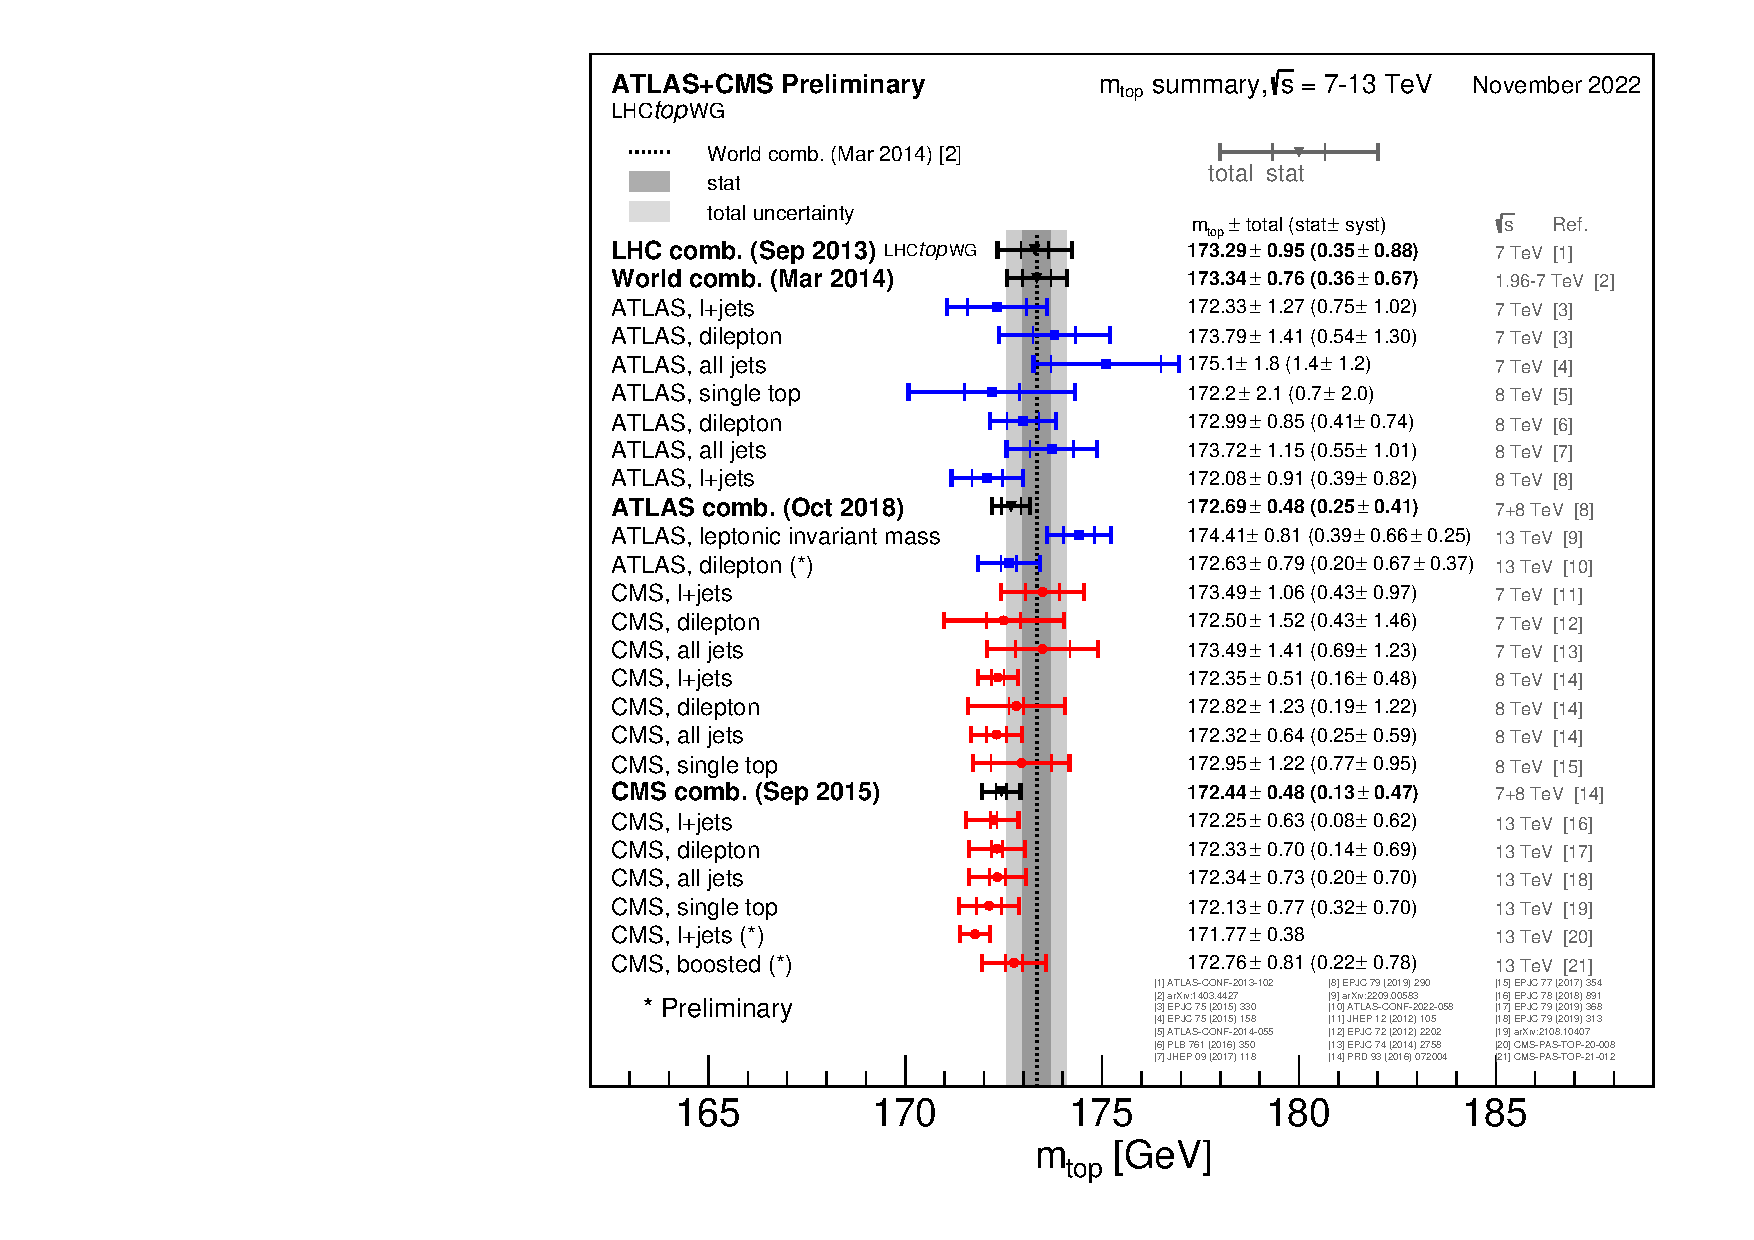
\includegraphics[width = 0.8\textwidth]{Chapter1/LHC_topMCmass_Nov22}
   	 \caption{Summary of the ATLAS and CMS $\mtop^{MC}$ measurements from top-quark decay. 
	 Results compared to Large Hadron (LHC) \mtop combination~\cite{ATLAS:2022lsz}. 
	 The most precisely studied property of the top quark is its mass.}
    	\label{fig:Chap1:top:mtop_MC}
	\end{figure}

	
       \item Indirect measurements~\cite{Amoroso:2746800}:
	The $\mtop^{\text{pole}}$ is measured from measurements of the cross-section. These methods
	rely on the dependence on the value of the $\mtop$ for the total or differential production 
	cross-sections for processes involving top quarks. Figure~\ref{fig:Chap1:top:mtop_Pole}
	presents $\mtop^{\text{pole}}$ indirect measurements.
	%$\rightarrow$ $m_{t}^{\text{pole}}$ with $O(1$~GeV$)$ precision
	\begin{figure}
    	\centering
    	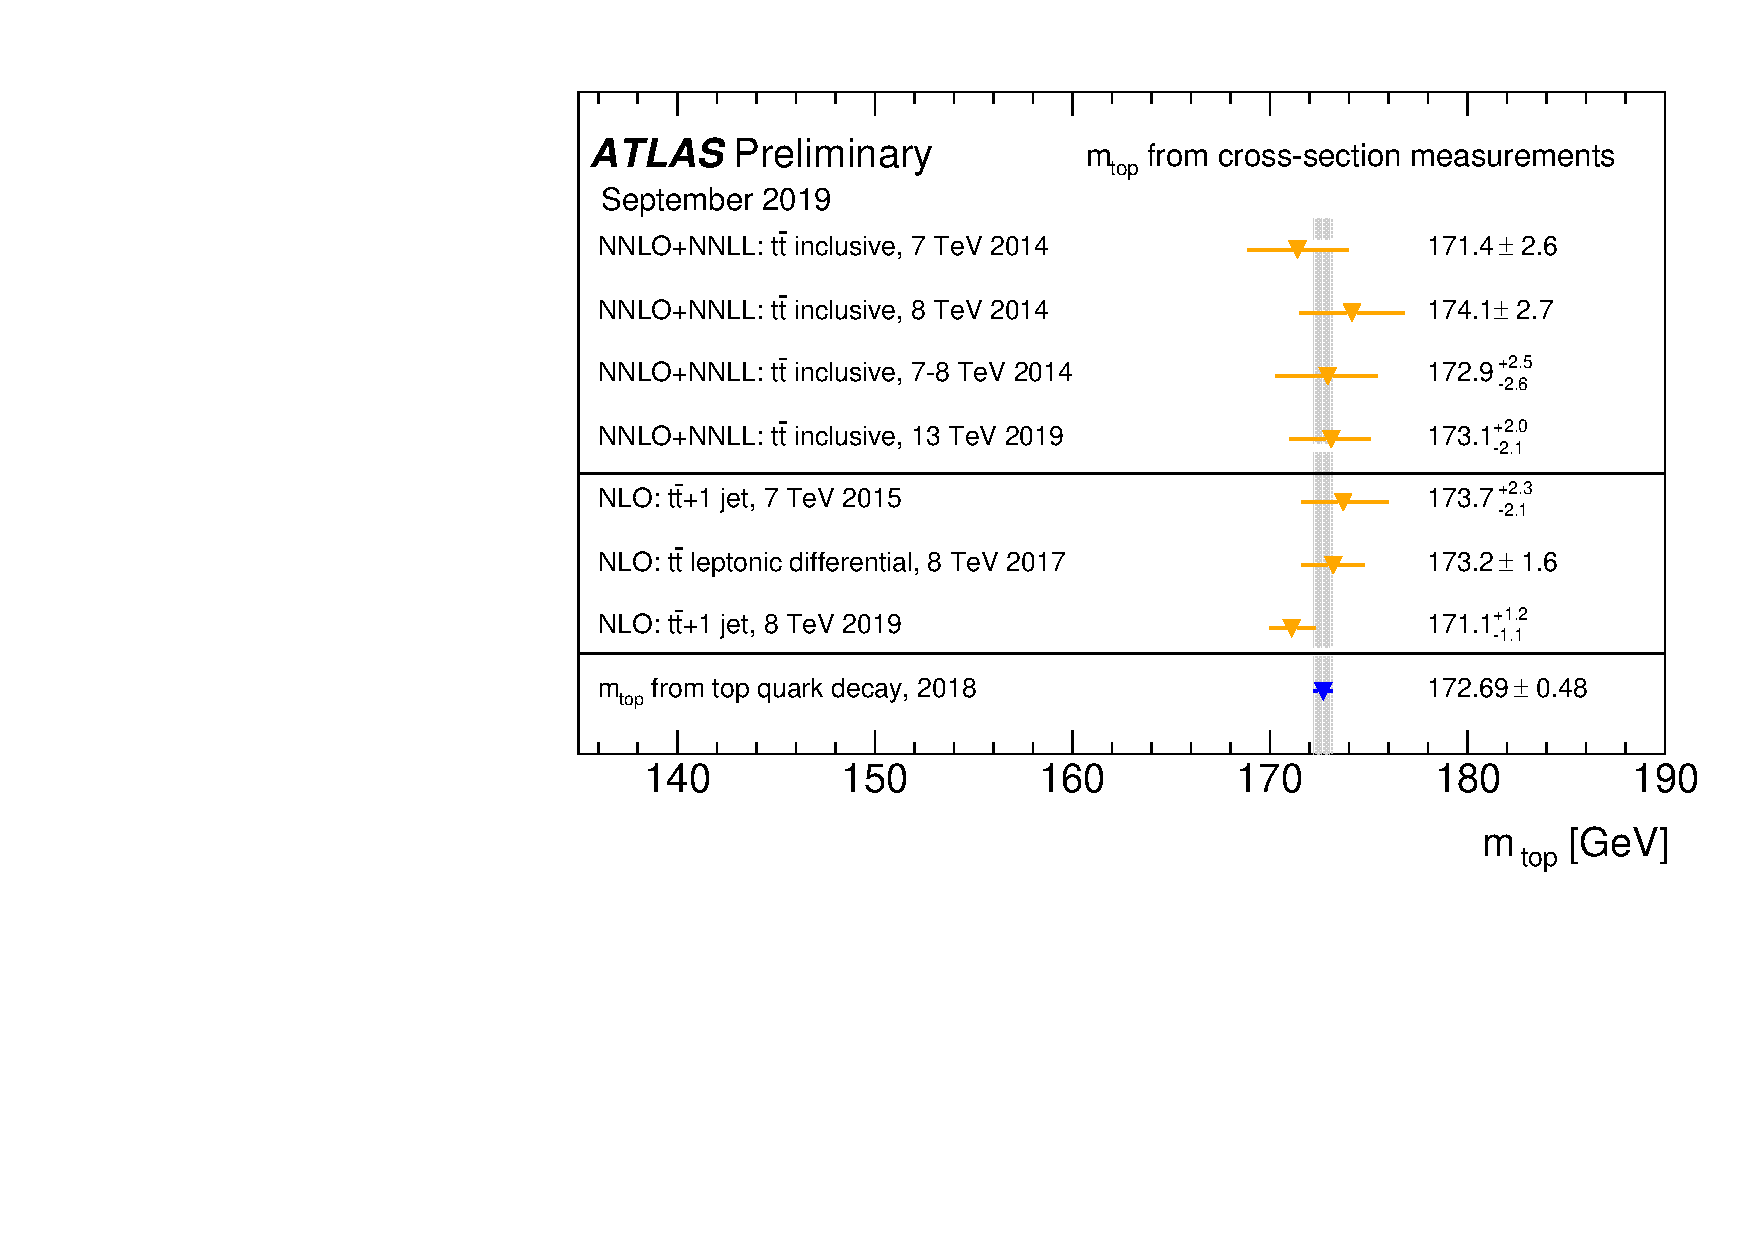
\includegraphics[width = 0.8\textwidth]{Chapter1/LHC_topPOLEmass_Sept19}
    	\caption{Summary of the measurements of the $\mtop^{\text{pole}}$ from \ttbar cross-section measurements.
    	A caparison to the measurements from top-quark decay is provided~\cite{ATLAS:2018fwq}.}
    	\label{fig:Chap1:top:mtop_Pole}
	\end{figure}
	\end{itemize} 	
	% ref:  	Strategy for ATLAS top quark mass measurements: 2021-2023
	%         	https://cds.cern.ch/record/2746800?


\pablo{No he explicado qué es  $\mtop^{MC}$ y  $\mtop^{\text{pole}}$. No hace falta, no?}
% La pole mass es la que sale en teoría
% La MC mass se mide de los hadrones que salen del top quark y no se entiende muy bien qué significa

\end{comment}

Among the properties of the top quark, its mass is the one that has received the most attention so far.
Accurate measurements of \mtop are vital for determining the parameters of the EW global fits, which are essential for evaluating the internal consistency of the SM and exploring its potential extensions~\cite{ALEPH:2010aa, Baak:2014ora}. Moreover, the \mtop value influences the stability of the Higgs-boson potential, carrying which has cosmological implications~\cite{Degrassi:2012ry, Bezrukov:2007ep, DeSimone:2008ei}.
The most recent studies for the top-quark mass measurements result in $\mtop = 172.76 \pm 0.30$~GeV~\cite{Workman:2022ynf}. %~\cite{pdgTop}. 
This number is an average of the measurements at the Large Hadron (LHC) 
with ATLAS ($172.69 \pm 0.66$~GeV~\cite{ATLAS:2018fwq})
and CMS ($172.6 \pm 2.5$~GeV at CMS~\cite{CMS:2019fak}) 
and at Tevatron with CDF and D$\emptyset$ (combined result: $174.30 \pm 0.89$~GeV~\cite{CDF:2016vzt}).
These values are measured from the kinematics of  \ttbar events and refer to the $\mtop^{\text{pole}}$.%\footnote{In 
	 %particle physics, an event is the result of a collision.}.%\footnote{This \mtop results are sensitive to the 
%top quark mass used in the MC generator that is usually interpreted as the pole mass.}.
% top masses: https://pdglive.lbl.gov/DataBlock.action?node=Q007TP
% Direct measurements    :: $\mtop^{\text{MC}}$
% Indirect measurements :: $\mtop^{\text{pole}}$
 
%Figure~\ref{fig:Chap1:top:mtop_tt}  presents the results for \mtop measurements from \ttbar observables.

% Definition of mass: 
% Quark masses are fundamental parameters of QCD.  In QFT, the propagator of a massive fermion has a pole
% at $m_0$ called the pole mass, which also corresponds to the invariant mass calculated from
% its decay products. However, the quarks present a particular situation due to its confinement.
% Most measurements are based on the invariant mass of the top quark decay products.
% The measured top quark mass has been interpreted as the pole mass by the Particle Data Group.
%  For all other quarks, in contrast, the renormalised masses are used.

%The high mass of the top quark indicate its Yukawa coupling to the Higgs field of $\mathcal{O}(1)$.

%\begin{figure}
%    \centering
%    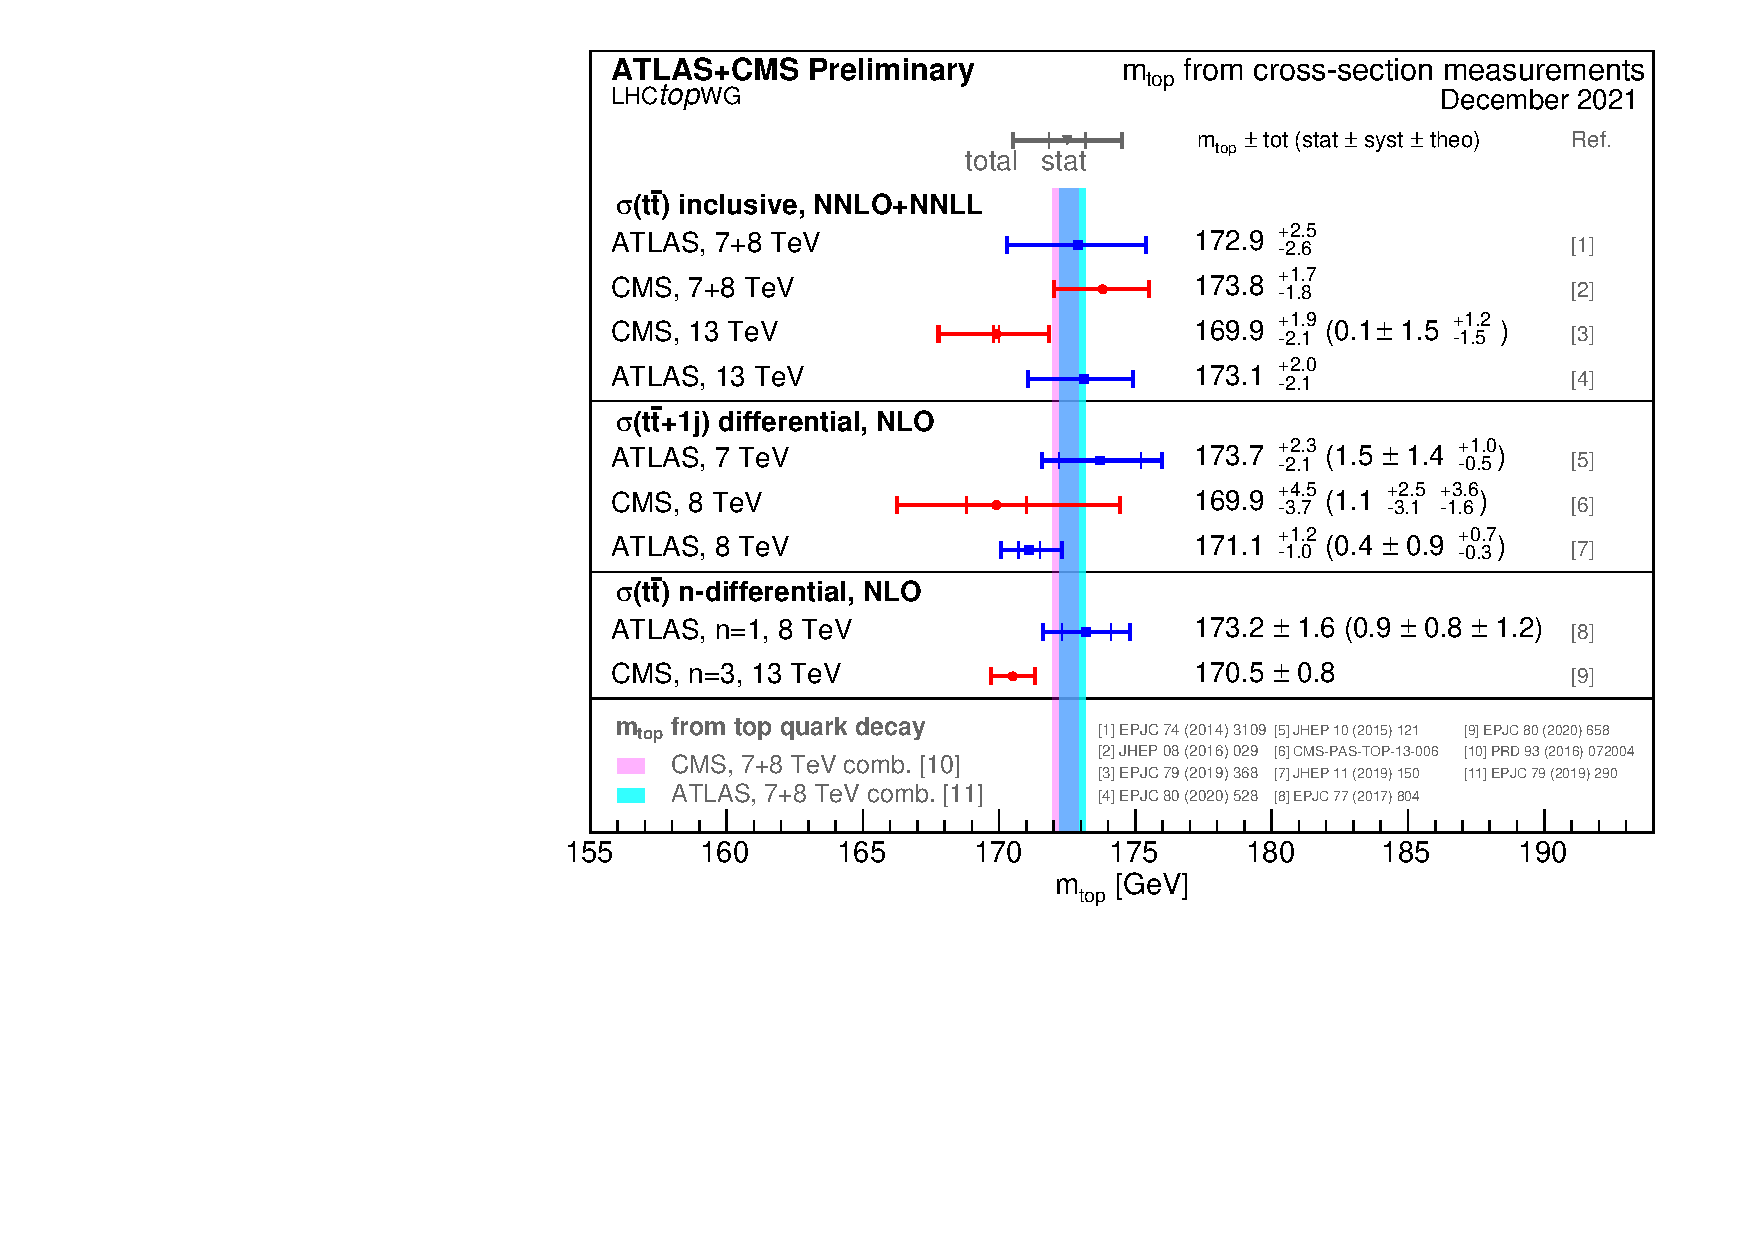
\includegraphics[width = 0.8\textwidth]{Chapter1/LHC_topmassfromXS_dec21}
%    \caption{Summary of the ATLAS and CMS measurements from \ttbar observables. 
%		Results compared to measurements from direct-top-quark decay.}
%    \label{fig:Chap1:top:mtop_tt}
%\end{figure}



% ATLAS		$\mtop = 172.69 \pm 0.25$(stat)$\pm 0.41$(syst) GeV
% CMS		$\mtop = 172.6 \pm 0.4$(stat)$\pm 1.6$(exp)$\pm 1.5$(model)  GeV
% Tevatron	$\mtop = 174.30 \pm 0.35$(stat)$\pm 0.54$(syst) GeV 




%%%%%%%%%%%%%%%%%%%%%%%%%%
%                Top quark production at LHC               %
%%%%%%%%%%%%%%%%%%%%%%%%%%
\subsection{Top-quark production at LHC}
\label{sec:Chap1:Top:Production}
The LHC is sometimes referred to as a top-quark factory due to its capacity to produce such particles in large quantities. 
In this collider, at proton--proton ($\Pproton\Pproton$) collisions, the top quark is mainly produced via
two mechanisms: through the strong interaction in top-quark--antiquark pairs (\ttbar), and by means of the \Wtb 
vertex of EW interaction in single top quarks. % associated with other particles.  
 Apart from the \ttbar (see Section~\ref{sec:Chap1:Top:Production:TopPairs}) and single top quark
(see Section~\ref{sec:Chap1:Top:Production:SingleTop}) productions, the associated \ttX and \tX 
productions play a role on producing top quarks (see Section~\ref{sec:Chap1:Top:Production:ttbar_plus_X} and 
Section~\ref{sec:Chap1:Top:Production:top_plus_X}, respectively).

Since top quarks often constitute a main background in other physics analyses, 
a better understanding of the properties of this particle will directly translate into improvements 
in those studies.

%%%%%%%%%%%%%%%%
%                Top pairs               %
%%%%%%%%%%%%%%%%        %https://twiki.cern.ch/twiki/bin/view/LHCPhysics/TtbarNNLO
\subsubsection{Top-quark--antiquark pairs production}
\label{sec:Chap1:Top:Production:TopPairs}
The production of \ttbar events is the largest source of production of top quarks in hadron collisions. This
process is one of the most important at LHC because it allows us to precisely study the properties of the top quark. 
Additionally, due to the dominance of this production mode, the \ttbar production is also a major background 
in many measurements and searches for rare processes as mentioned above. 
The physics analysis carried out in this thesis is a good example, 
where the \ttbar process is the main background in
both of the analysed decay channels.

For proton--antiproton ($\Pproton \APproton$) collisions at Tevatron or $\Pproton \Pproton$ at LHC, the \ttbar production is described by
perturbative QCD.  In this approach, a hard scattering process between the two hadrons is the result 
of an interaction between the quarks and gluons that constitute these hadrons. This model is described in detail in 
Section~\ref{sec:Chap2:PhenoOfPP}.


At LHC, gluon fusion dominates with 90\% of 
the \ttbar production. It is followed by the quark--antiquark annihilation, 
which accounts for 10\% of the total \ttbar production.
%Due to its primordial importance for the physics programme of LHC
The theoretical calculations for the \ttbar 
production at $\CM=13\,\text{TeV}$ are done to an accuracy of  next-to-next-to-leading order (NNLO)
in QCD and complemented with next-to-next-to-leading logarithmic (NNLL) resummation~\cite{Czakon_2020, Czakon:2013goa}: %\cite{Czakon:2013tha}
\begin{equation*}
\sigma^{\text{pred}}_{\text{NLO+NNLL}}(\ttbar) = 833.9^{+20.5}_{-30.0}\text{(scale)}\,\pm 21.0 \text{(PDF}+\alpha_{s}) \, ^{+22.5}_{-23.2}\text{(mass)}\,\text{pb}\,. 
\end{equation*}
% ref: https://twiki.cern.ch/twiki/bin/view/LHCPhysics/TtbarNNLO
%\pablo{(En el paper de Czakon te pone la $\sigma^{pred}_{\ttbar}$ a 14 GeV y luego un plot de $\sigma^{pred}_{\ttbar}$ vs $\CM$ pero no da numerito a 13 TeV. Tampoco hay numerito en~\cite{ATLAS:2022uqj}. El número lo saco de~\cite{ATLAS:2022qak} quien lo saca de )}
Here, PDF stands for parton distribution function and $\alpha_{s}$ is the strong coupling constant.
The scale uncertainty refers to the sensitivity to the choice of factorisation and renormalisation 
scales\footnote{In QCD and QED, the renormalisation scale is a parameter that helps 
to eliminate infinities arising in the calculations of  interactions. It is associated with the 
energy scale at which a physical process occurs.}~\cite{Czakon:2016dgf}. 
These scales are further discussed in Section~\ref{sec:Chap2:PhenoOfPP:ProtonStructure}.
The ATLAS and CMS collaborations have measured its cross-section through different final state channels and 
the most precise result obtained so far at $\sqrt{s}=13$~TeV is~\cite{ATLAS:2023gsl} 
\begin{equation*}
\sigma^{\text{obs}} (\ttbar) = 829 \pm 1\text{(stat.)}\,\pm 13\text{(syst.)}\,\pm 8\text{(lumi.)}\, \text{pb} \, .
\end{equation*}
Thanks to this large cross-section, the statistical uncertainty is not constraining the measurements of
the \ttbar production, which is performed with good precision ($\mathcal{O}(2\%)$).
This large cross-section also makes \ttbar the most relevant background in this analysis.
%Figure~\ref{fig:Chap1:top:topPairs:CrossSection} 
%its most
%recent result are, respectively, $\sigma_{\ttbar} = 836 $$\pm$$ 29$~pb~\cite{ATLAS:2022qak} and $\sigma_{\ttbar} = 791 $$\pm$$ 36$~pb~\cite{CMS:2021vhb}. 
%shows the measurements for the \ttbar production cross-section ($\sigma_{\ttbar}$) at
%\CM =$13$~TeV.
%The measurements and the theory calculations are quoted at $\mtop=172.5$~GeV.
% At Tevatron, gluon fusion was not so important, as they had proton-antiproton collisions. 


%\begin{comment}
%\begin{figure}
%\begin{minipage}[c]{0.74\linewidth}
%\subfloat[\label{fig:Chap1:top:topPairs:FeynmanB1}]
%  {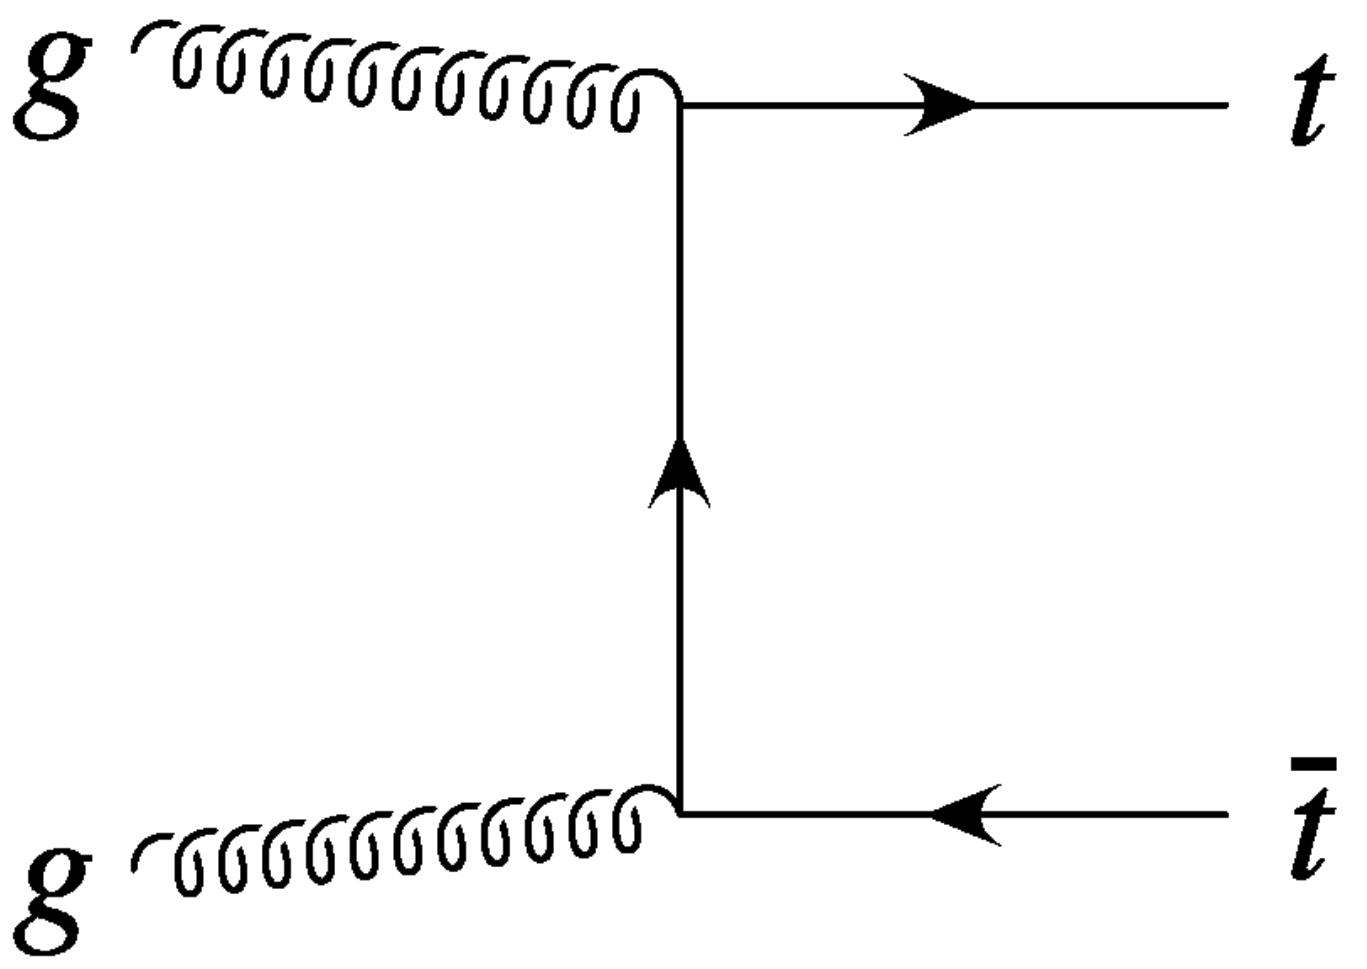
\includegraphics[width=.3\linewidth]{Chapter1/TopQuarkPairsFeynman-B1}}\hfill
%\subfloat[\label{fig:Chap1:top:topPairs:FeynmanB2}]
%  {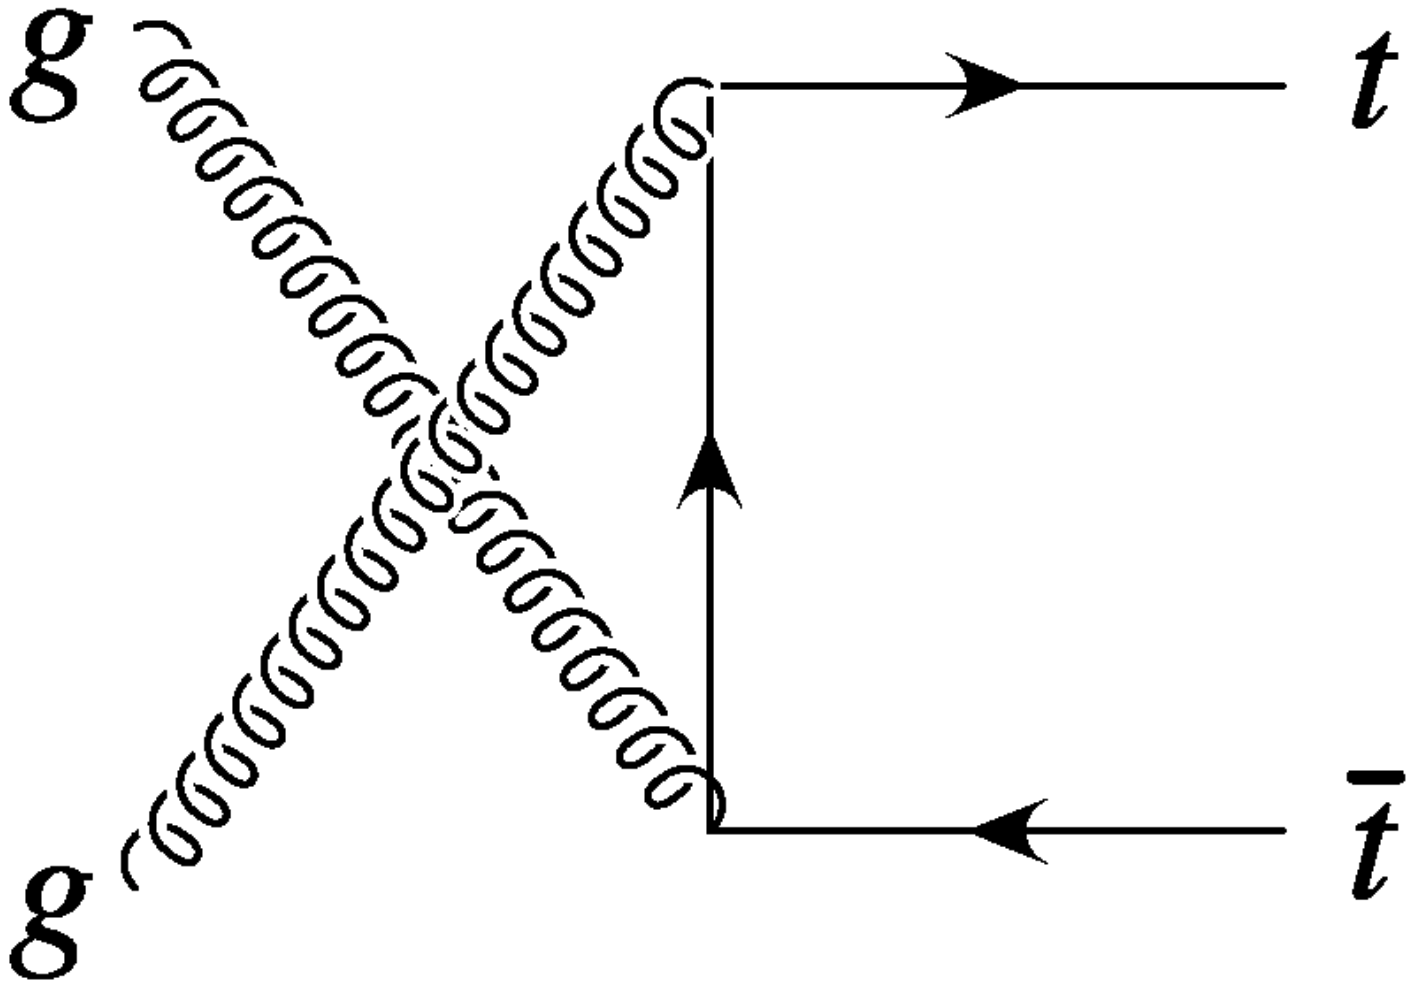
\includegraphics[width=.3\linewidth]{Chapter1/TopQuarkPairsFeynman-B2}}\hfill
%\subfloat[\label{fig:Chap1:top:topPairs:FeynmanB3}]
%  {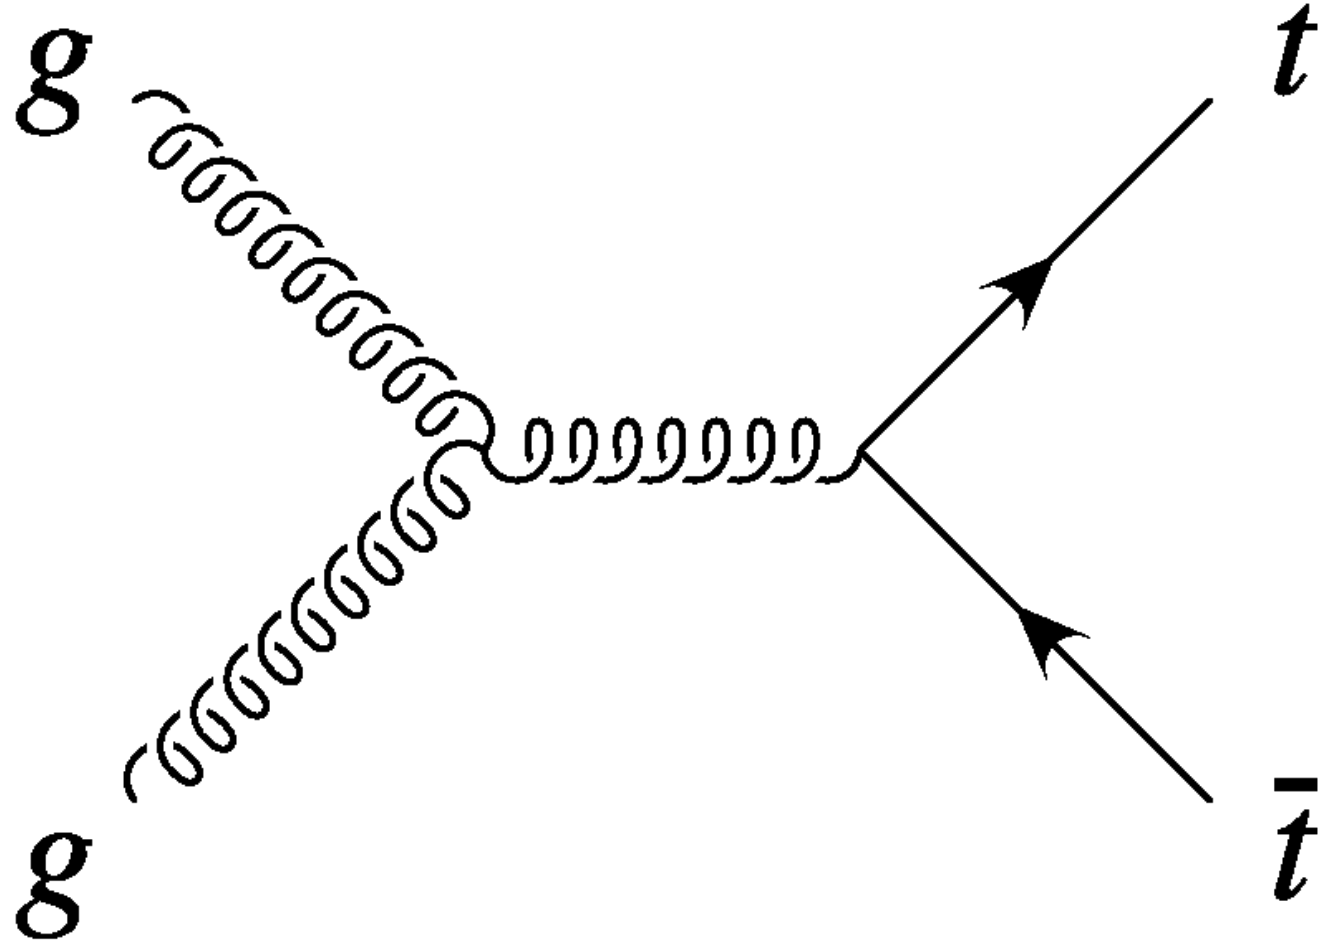
\includegraphics[width=.3\linewidth]{Chapter1/TopQuarkPairsFeynman-B3}}\hfill
%\caption{Representative Feynman diagrams of the LO processes contributing to the \ttbar 
%	production through gluon fusion at LHC.}
%\label{fig:Chap1:top:topPairs:FeynmanB}
%\end{minipage}
%\hfill
%\begin{minipage}[c]{0.25\linewidth}
%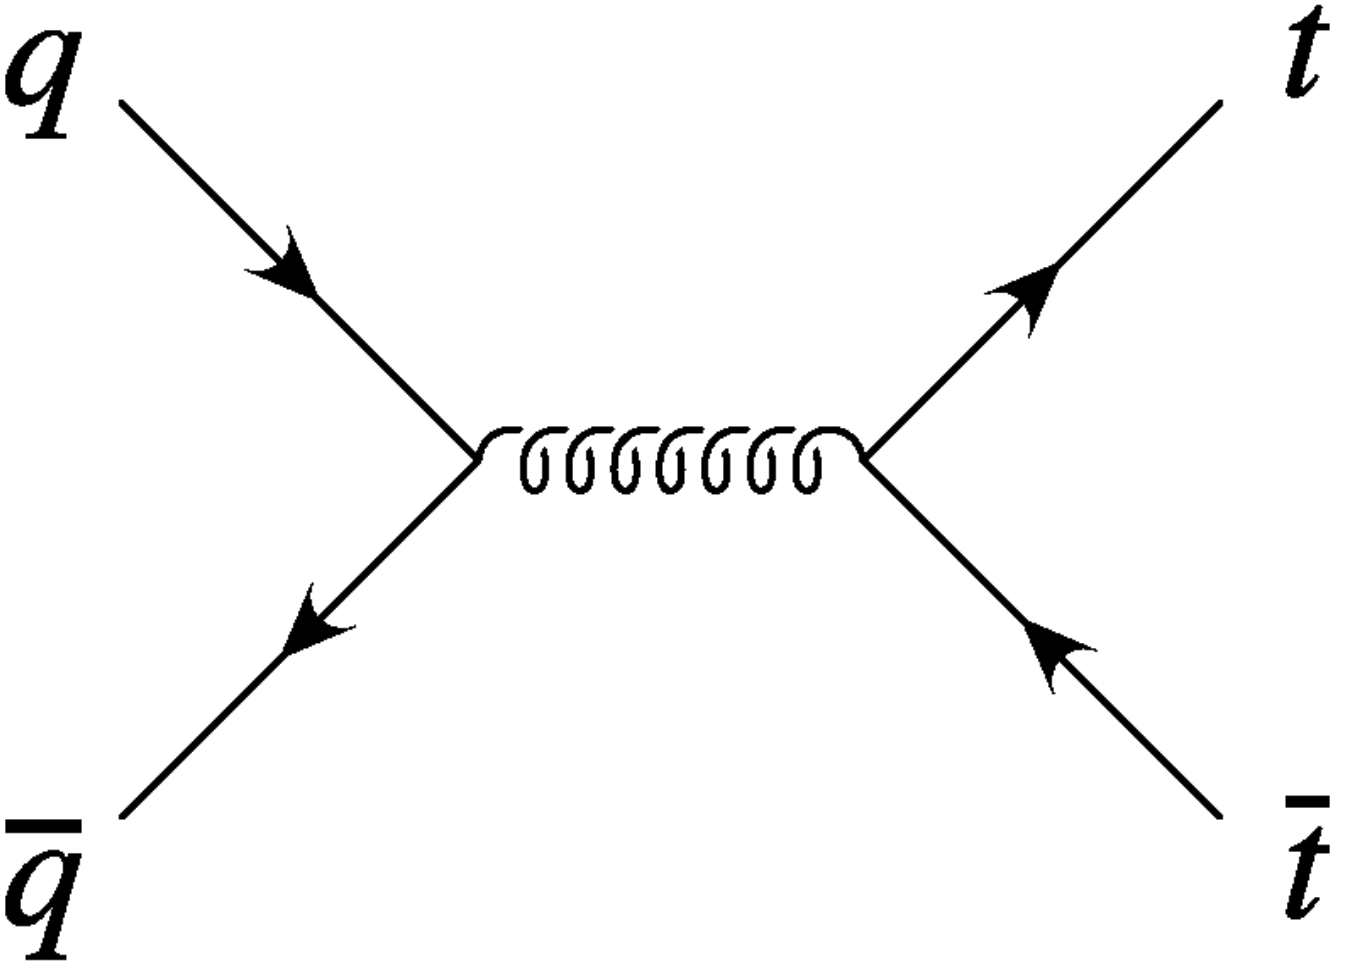
\includegraphics[width = 0.99\textwidth]{Chapter1/TopQuarkPairsFeynman-A}
%    \caption{LO Feynman diagram for \ttbar production 
%    		via quark and anti-quark annihilation.}
%    \label{fig:Chap1:top:topPairs:FeynmanA}
%\end{minipage}%
%\end{figure}
%\end{comment}

\begin{comment}
\begin{figure}
\begin{subfigure}[h]{0.23\linewidth}
	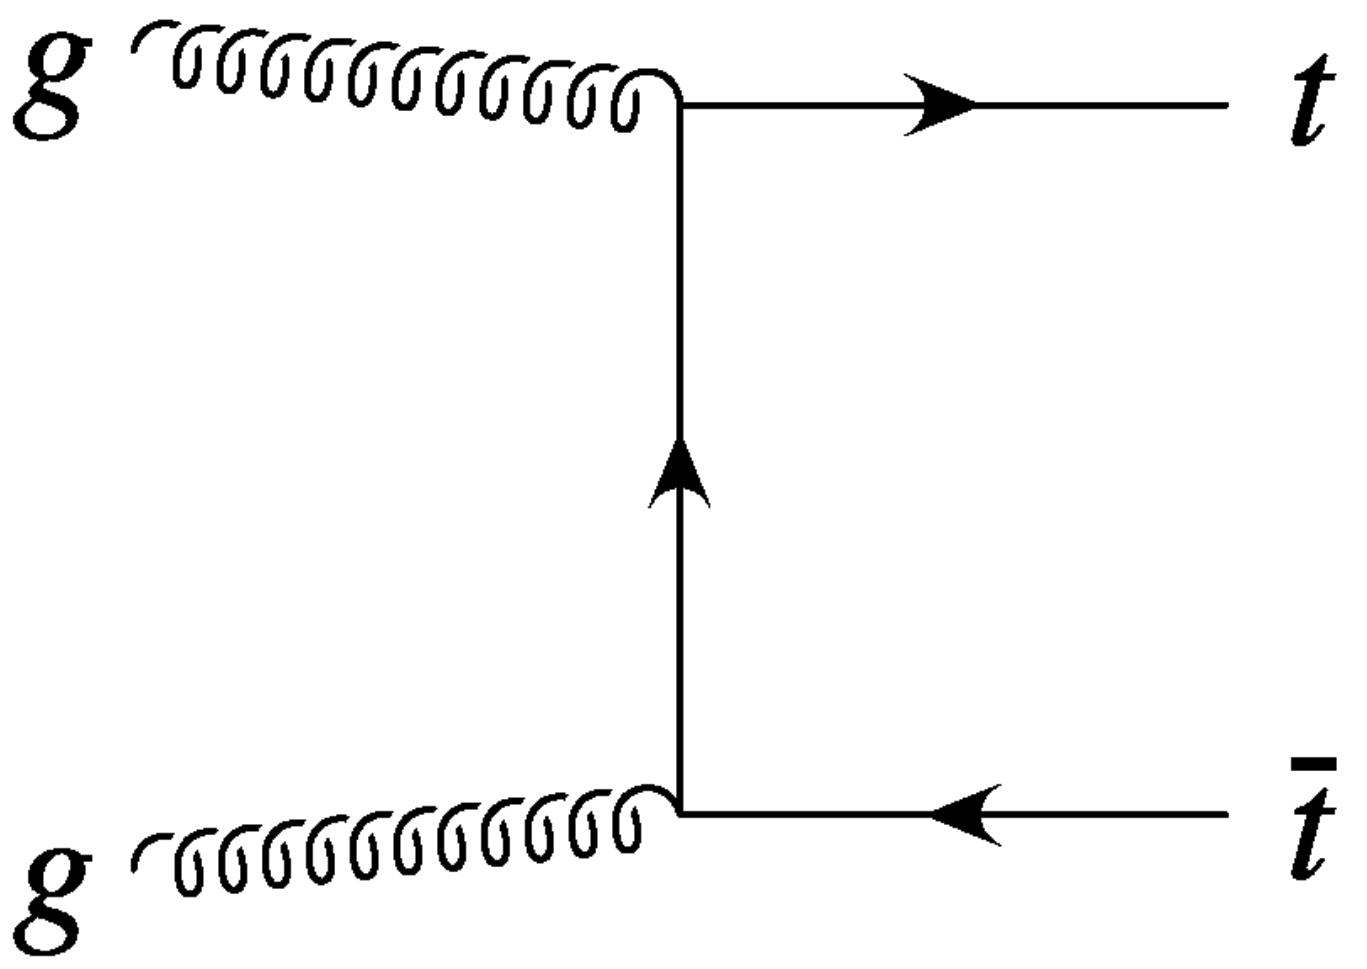
\includegraphics[width=\linewidth]{Chapter1/TopQuarkPairsFeynman-B1}
	\caption{}
	\label{fig:Chap1:top:topPairs:FeynmanB1}
\end{subfigure}
\hfill
\begin{subfigure}[h]{0.23\linewidth}
	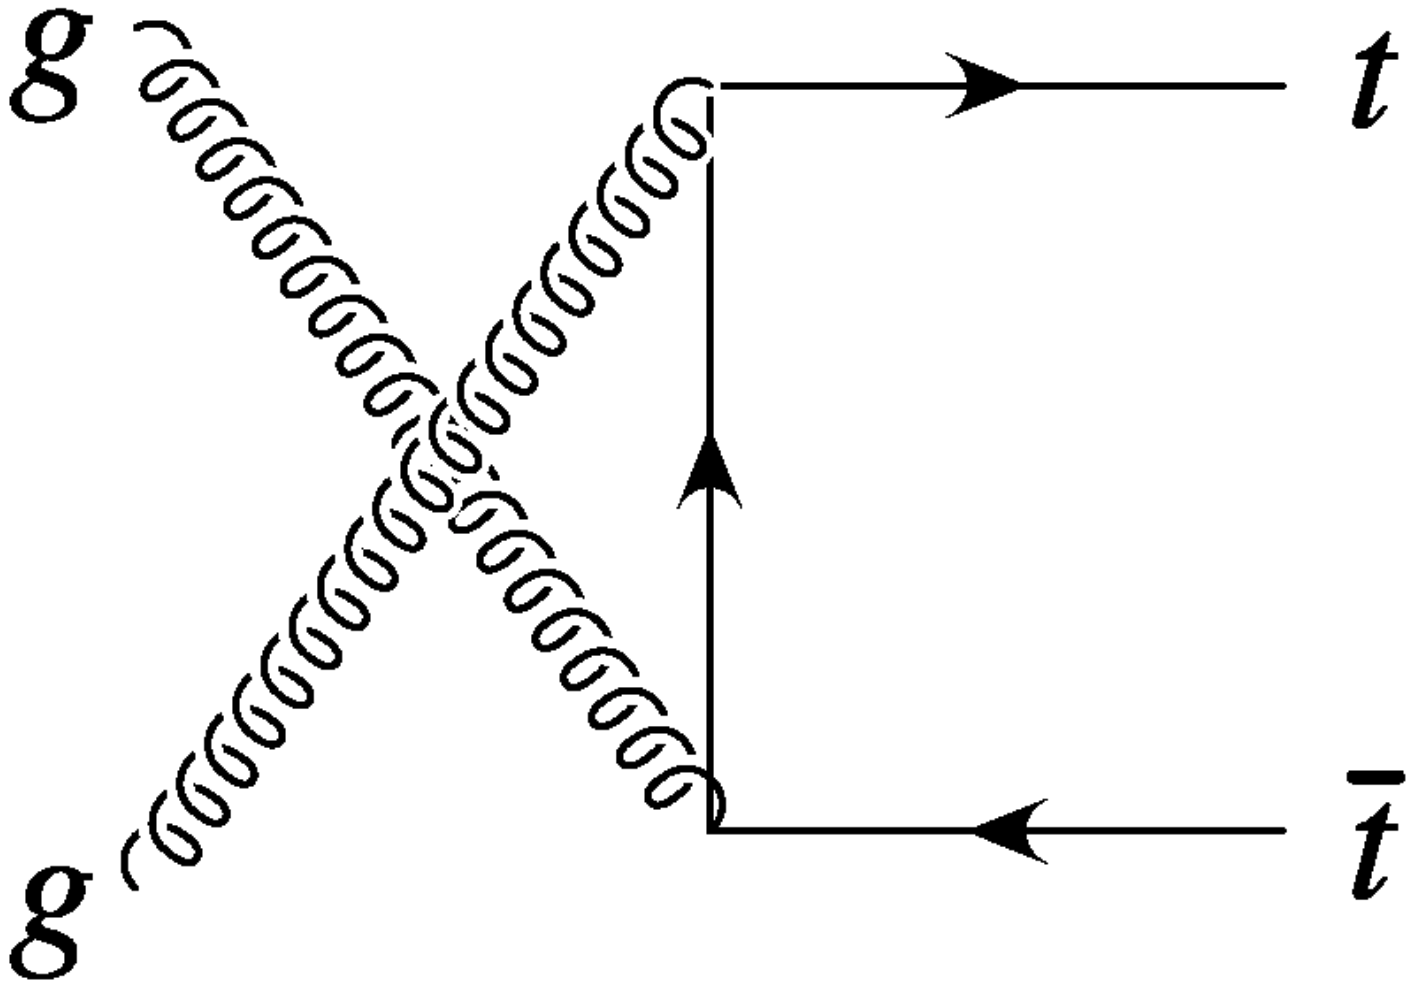
\includegraphics[width=\linewidth]{Chapter1/TopQuarkPairsFeynman-B2}
	\caption{}
	\label{fig:Chap1:top:topPairs:FeynmanB2}
\end{subfigure}
\hfill
\begin{subfigure}[h]{0.23\linewidth}
	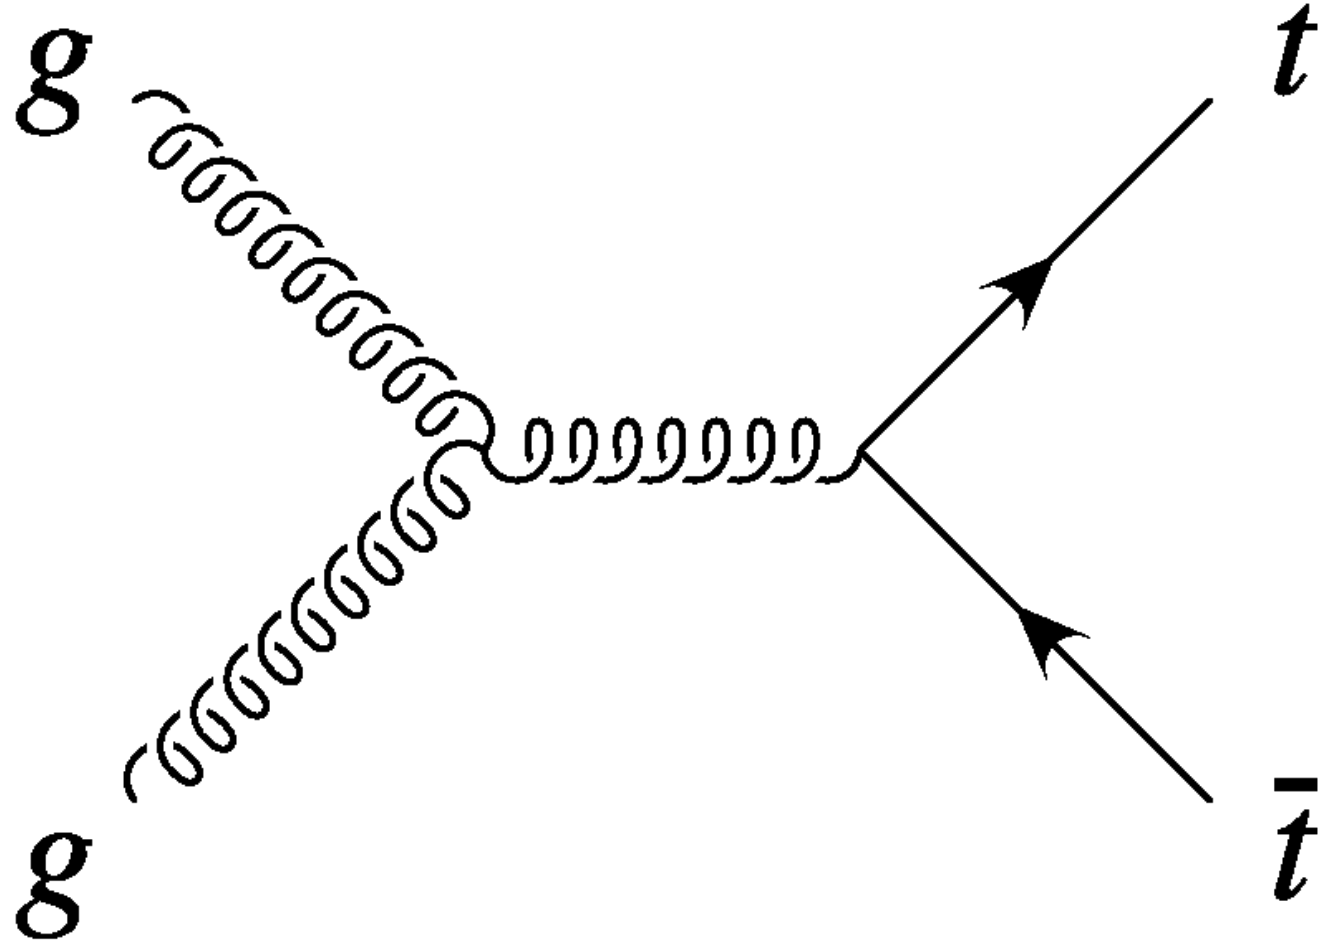
\includegraphics[width=\linewidth]{Chapter1/TopQuarkPairsFeynman-B3}
	\caption{}
	\label{fig:Chap1:top:topPairs:FeynmanB3}
\end{subfigure}
\hfill
\begin{subfigure}[h]{0.25\linewidth}
	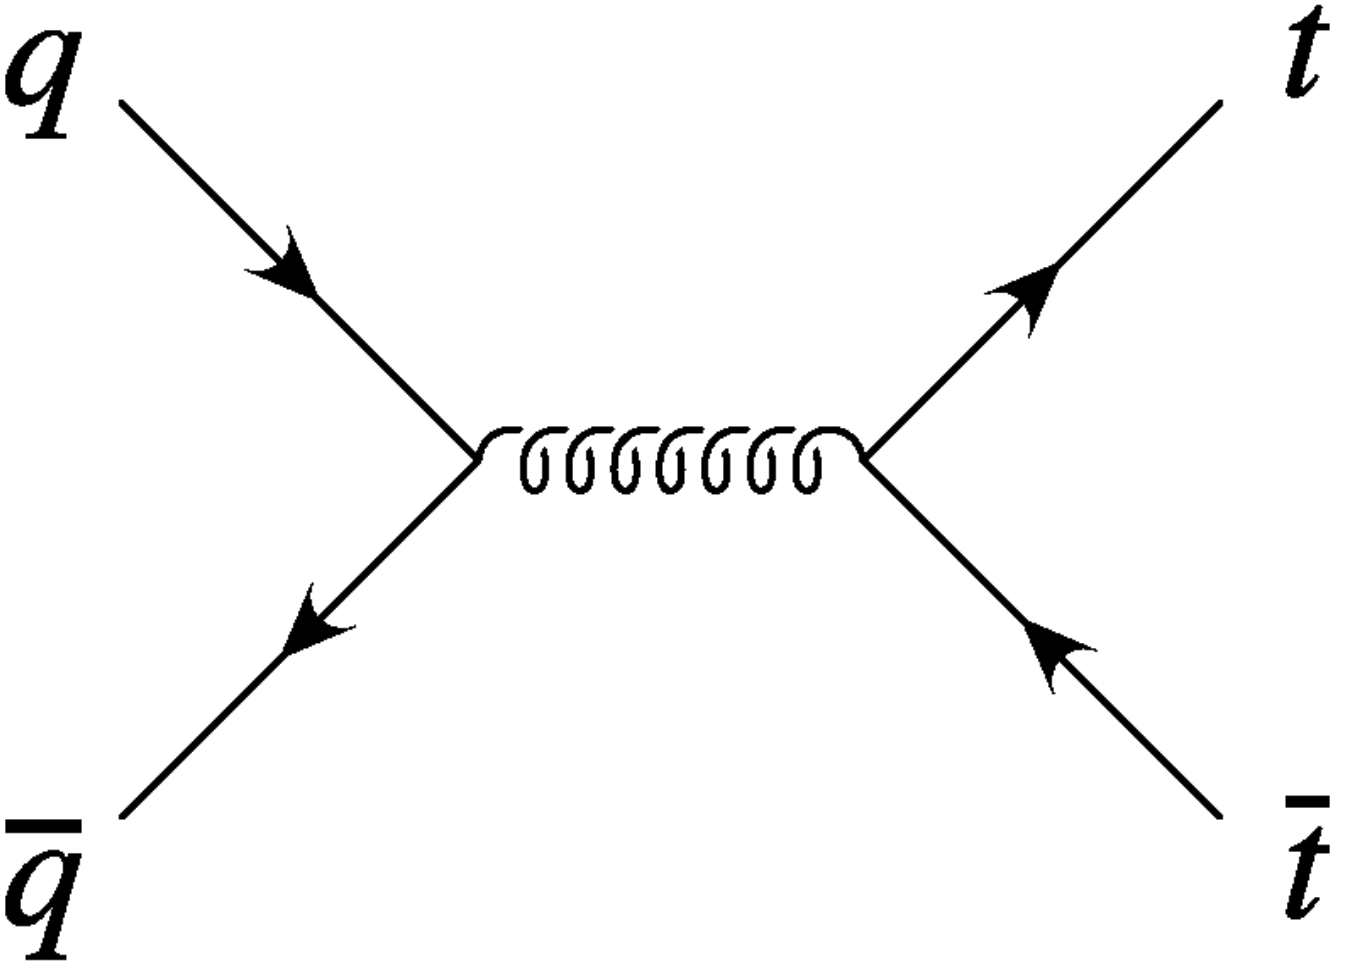
\includegraphics[width=\linewidth]{Chapter1/TopQuarkPairsFeynman-A}
	\caption{}
	\label{fig:Chap1:top:topPairs:FeynmanA}
\end{subfigure}%
\caption{Representative Feynman diagrams of the LO processes contributing to the \ttbar 
production. Where (a), (b) and (c) correspond to the production through gluon fusion 
and (d) to the production via quark--antiquark annihilation.}
\label{fig:Chap1:top:topPairs:Feynman}
\end{figure}
\end{comment}



%\begin{figure}
%\subfloat[\label{fig:Chap1:top:topPairs:FeynmanB1}]
%  {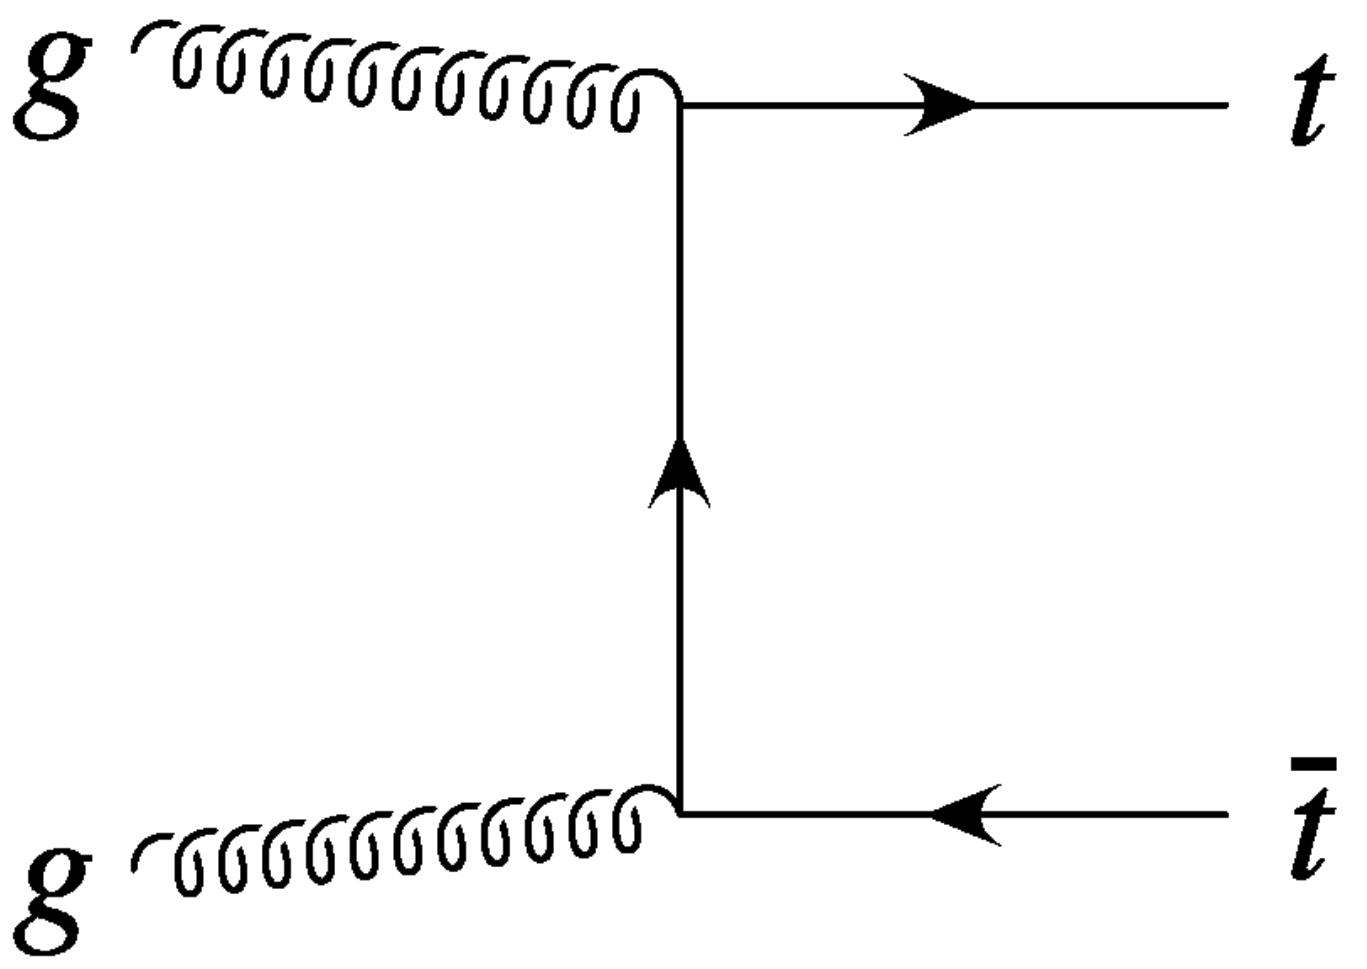
\includegraphics[width=.3\linewidth]{Chapter1/TopQuarkPairsFeynman-B1}}\hfill
%\subfloat[\label{fig:Chap1:top:topPairs:FeynmanB2}]
%  {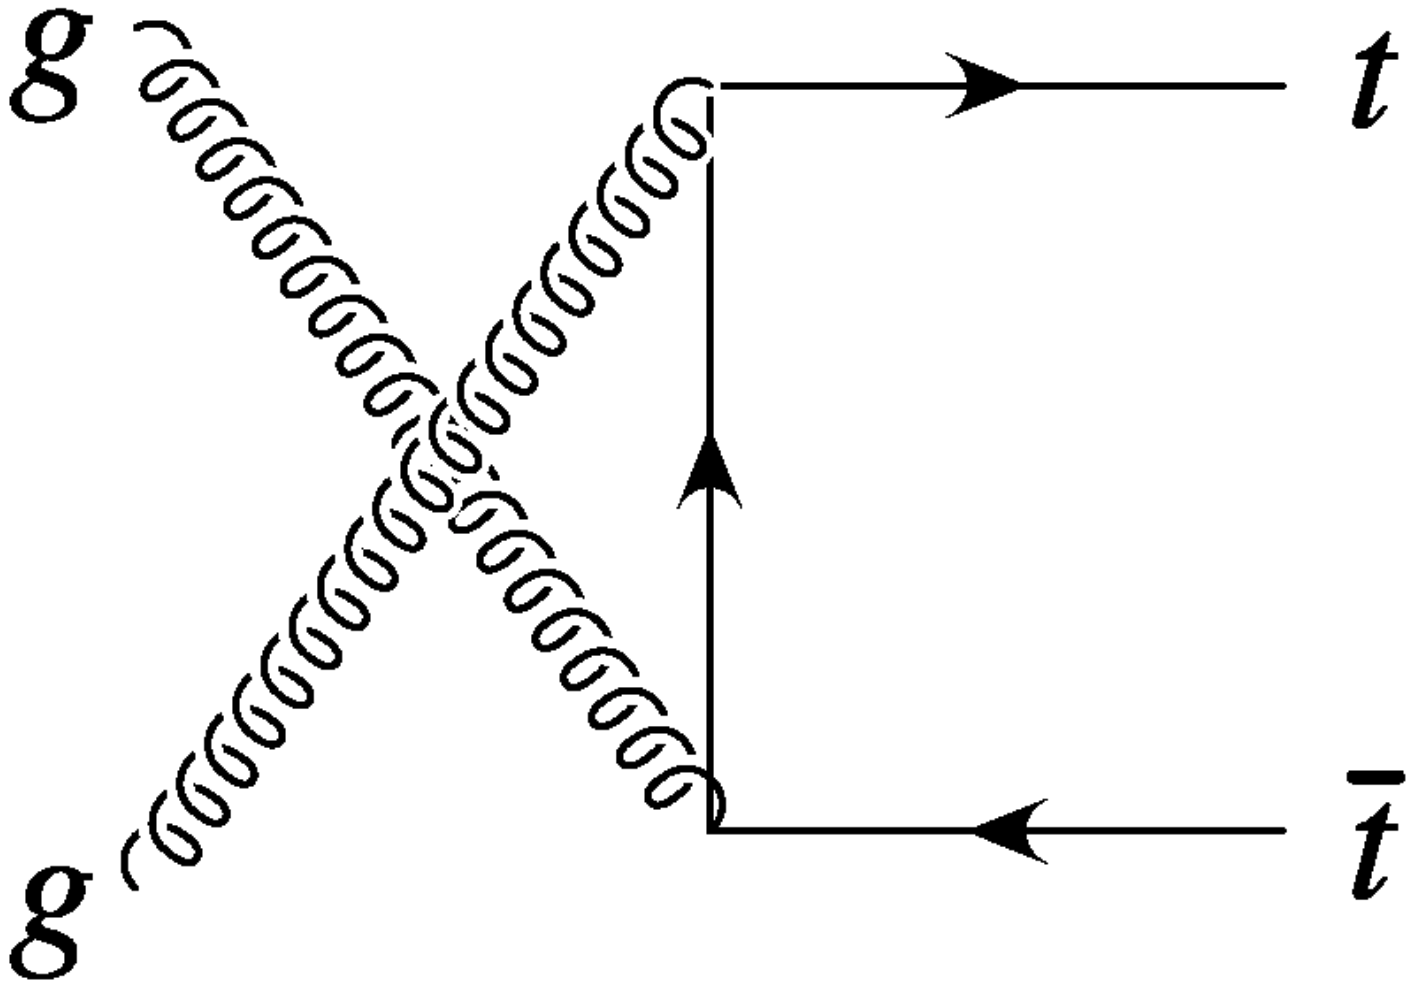
\includegraphics[width=.3\linewidth]{Chapter1/TopQuarkPairsFeynman-B2}}\hfill
%\subfloat[\label{fig:Chap1:top:topPairs:FeynmanB3}]
%  {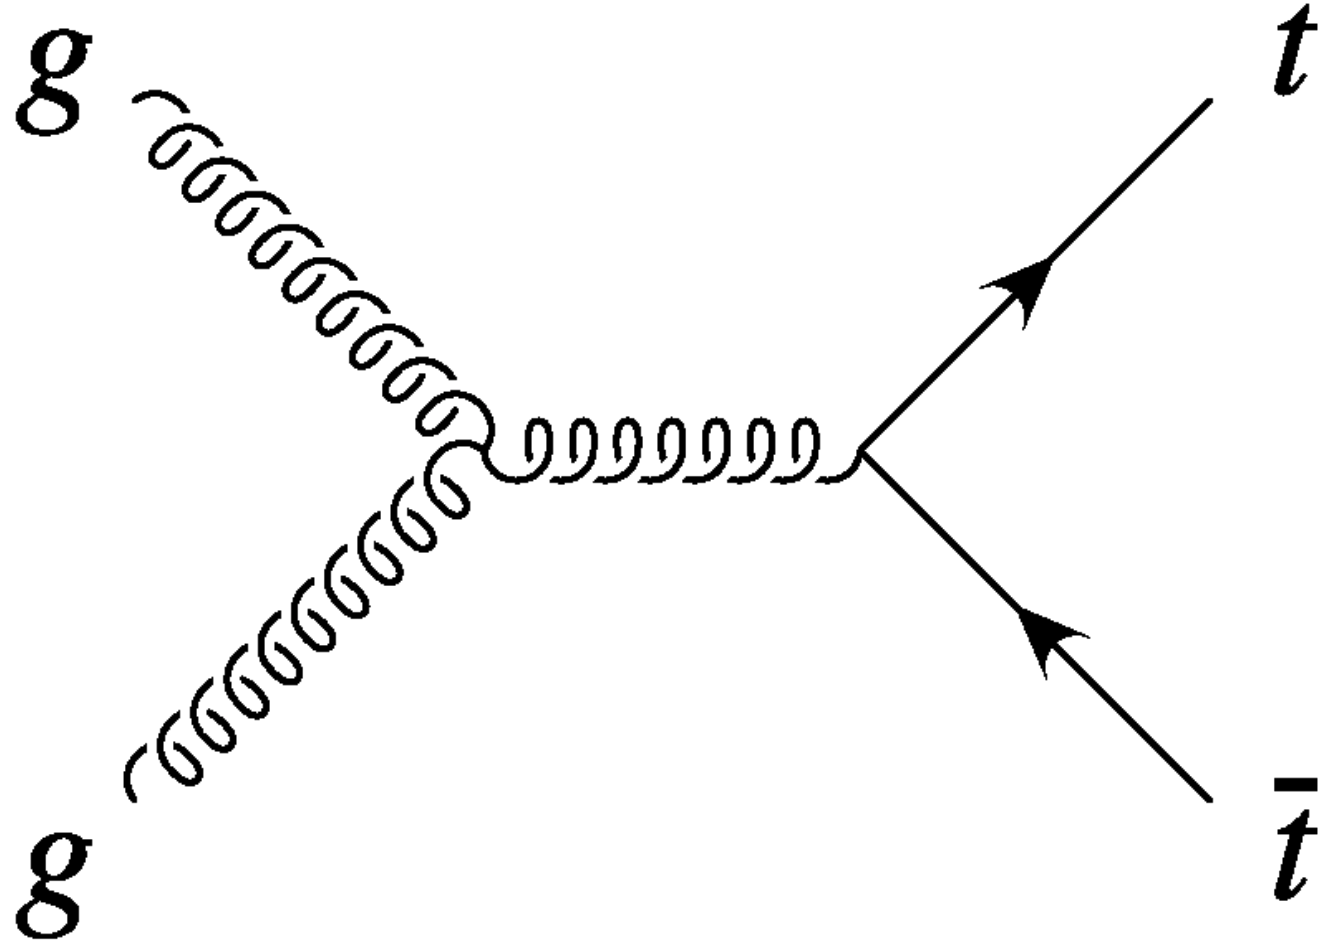
\includegraphics[width=.3\linewidth]{Chapter1/TopQuarkPairsFeynman-B3}}\hfill
%\caption{Representative Feynman diagrams of the LO processes contributing to the \ttbar production via gluon fusion at LHC.}
%\label{fig:Chap1:top:topPairs:FeynmanB}
%\end{figure}

%\begin{figure}
%    \centering
%    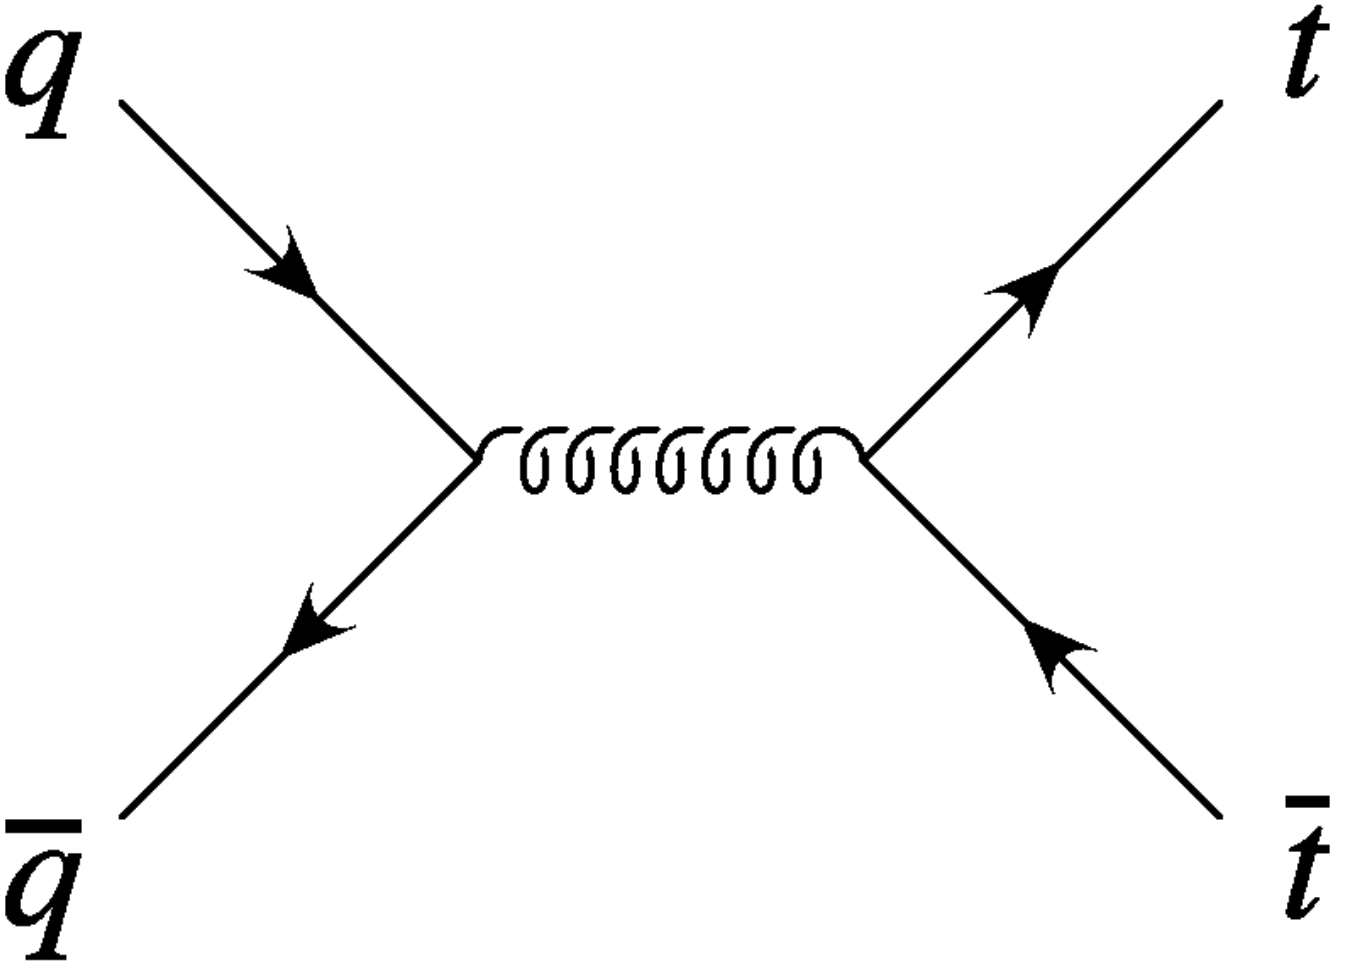
\includegraphics[width = 0.4\textwidth]{Chapter1/TopQuarkPairsFeynman-A}
%    \caption{Representative Feynman diagrams of the LO processes contributing to 
%    		the \ttbar production at LHC through quark and anti-quark annihilation.}
%    \label{fig:Chap1:top:topPairs:FeynmanA}
%\end{figure}

%\begin{figure}
%    \centering
%    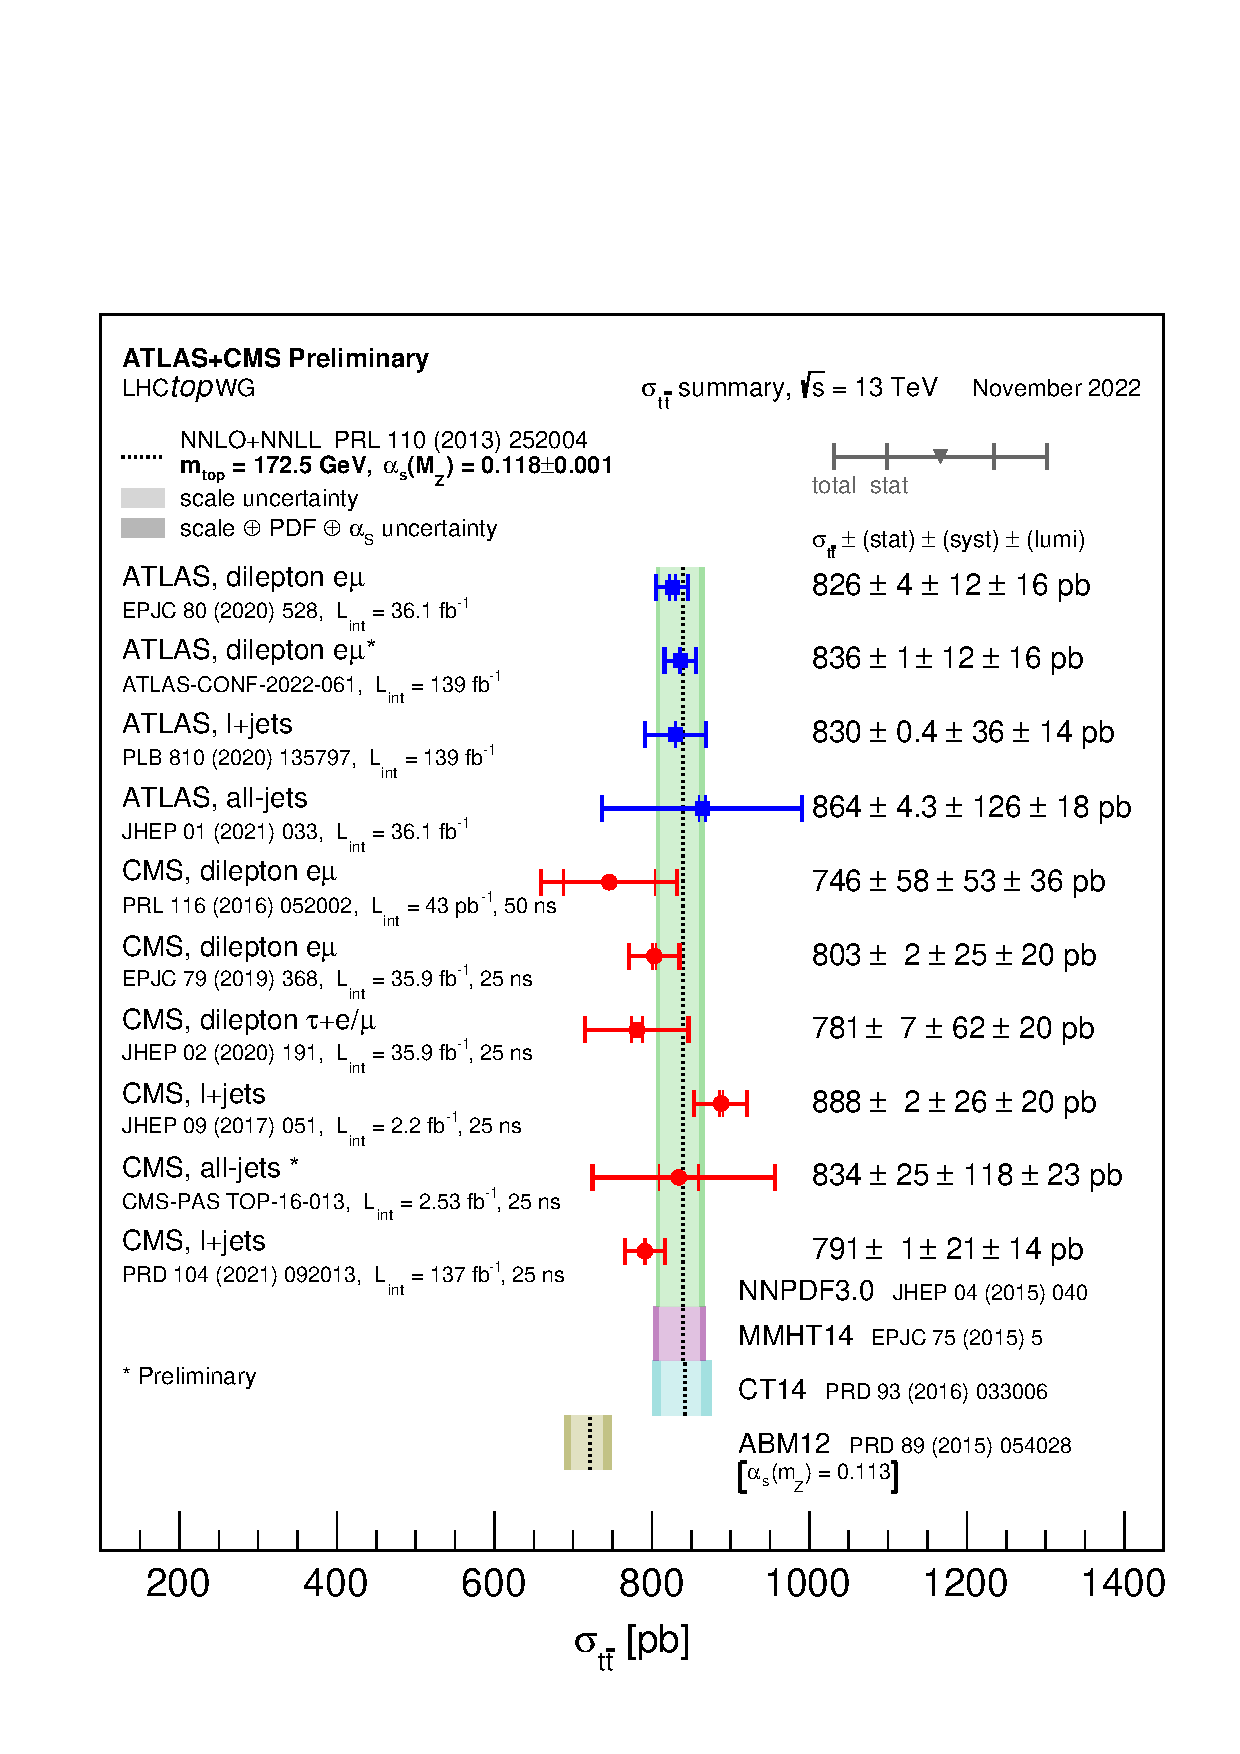
\includegraphics[width = 0.75\textwidth]{Chapter1/tt_xsec_13TeV_nov22}
%    \caption{Summary of measurements $\sigma_{\ttbar}$ at $\CM=13$~TeV compared to 
%    		the exact NNLO QCD calculation complemented with next-to-next-to-leading logarithmic resummation %\cite{ATLAS:2022uqj}. \pablo{Susana sugiere eliminar estas tablas}}
		%Update from https://twiki.cern.ch/twiki/bin/view/LHCPhysics/LHCTopWGSummaryPlots#Pair_production_cross_section
%    \label{fig:Chap1:top:topPairs:CrossSection}
%\end{figure}

%\begin{figure}
%    \centering
%    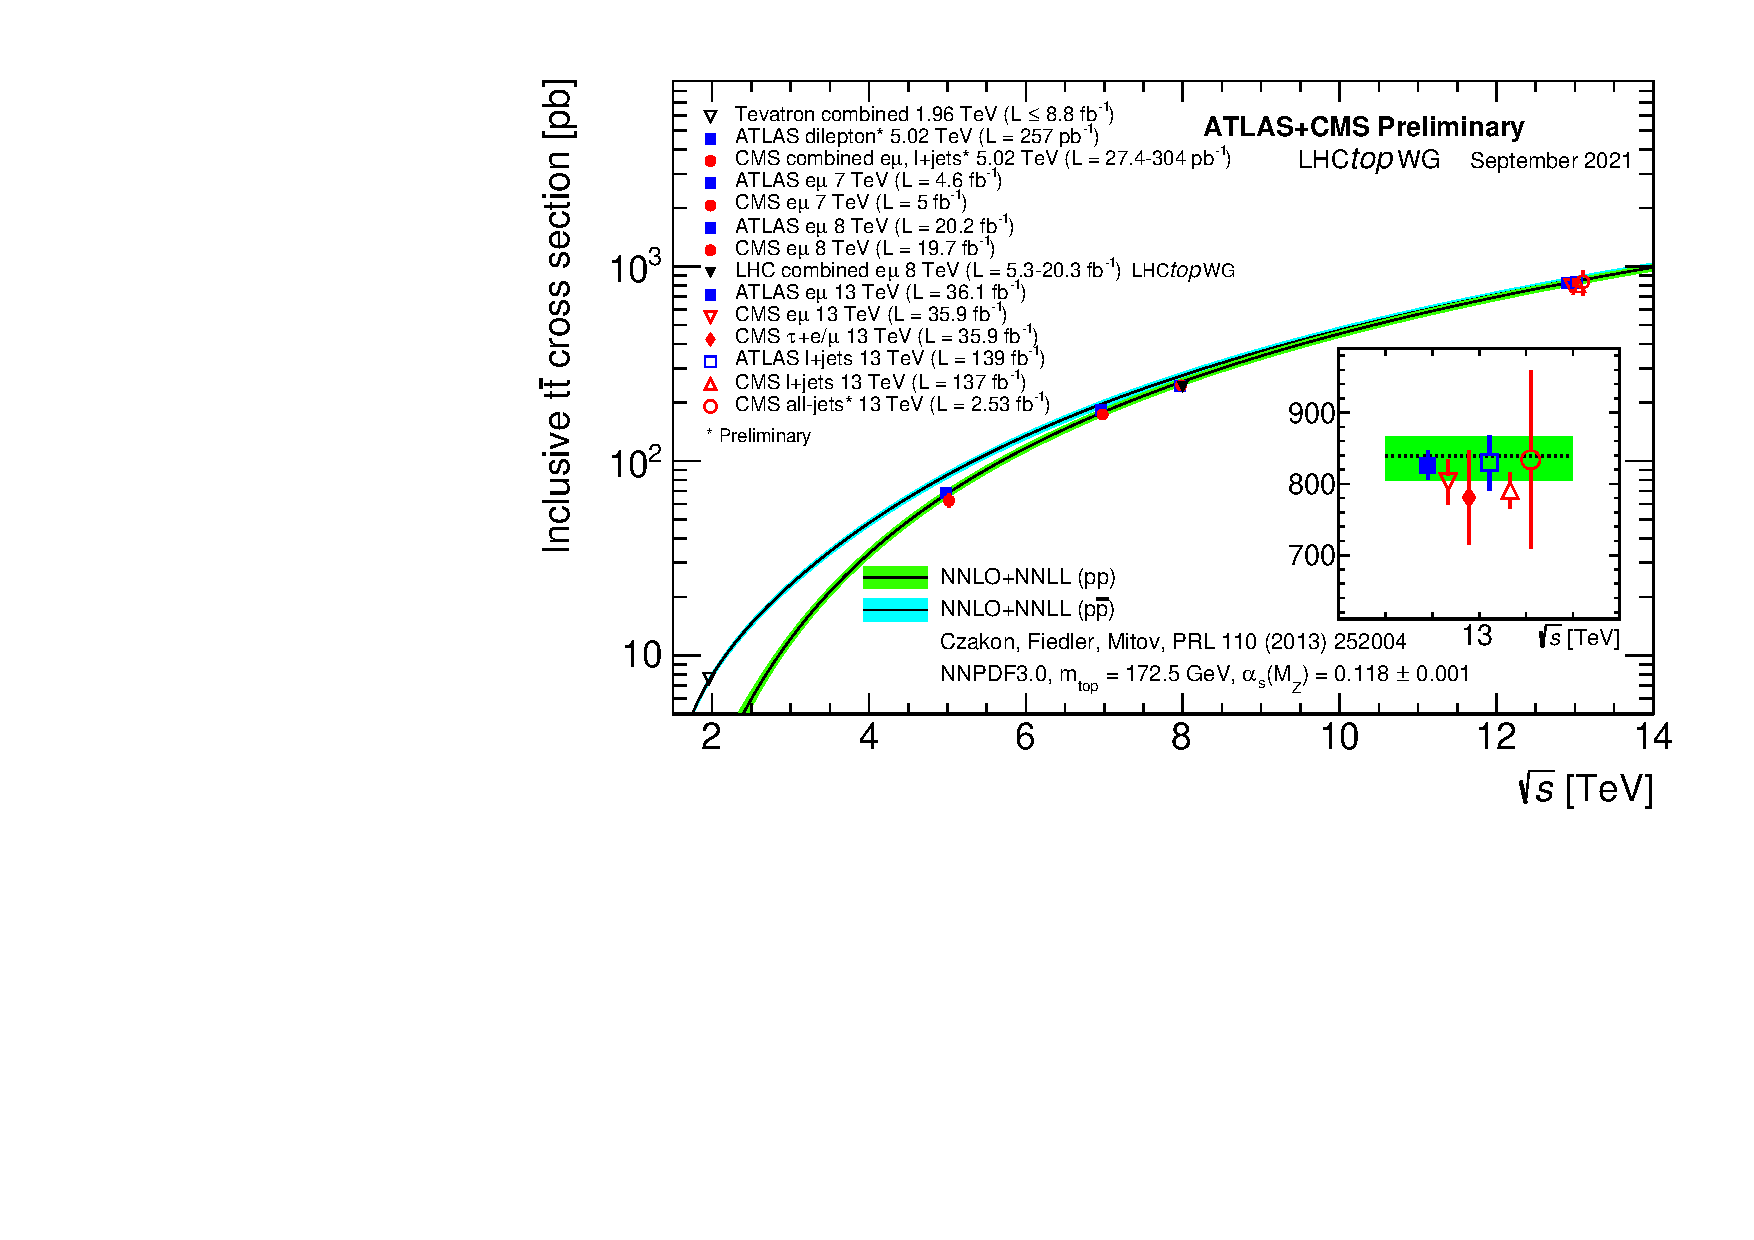
\includegraphics[width = 0.75\textwidth]{Chapter1/tt_curve_toplhcwg_sep21}
%    \caption{Summary of LHC and Tevatron measurements of the top-pair production cross-section as a function of the centre-of-mass energy}
    % The measurements and the theory calculation are quoted at mtop=172.5 GeV.
%    \label{fig:Chap1:top:topPairs:CrossSection_vs_CM}
%\end{figure}


%%%%%%%%%%%%%%%%%%%%
%                Single-top quark               %
%%%%%%%%%%%%%%%%%%%%
\subsubsection{Single-top-quark production}
\label{sec:Chap1:Top:Production:SingleTop}
In addition to the \ttbar production, the single-top-quark production is of great 
importance to the study of the top-quark properties at the LHC.  
This mechanism has a cross-section about three times smaller than that of \ttbar processes and  
it is almost exclusively produced through the EW interaction.
This is precisely the reason why single-top-quark production is essential to gather 
information about the \Wtb interaction and to directly measure the CKM
matrix element $|V_{tb}|$ at hadron colliders.
The reason why the single top quark is produced and decays via a $\Pbottom$-quark
%The reason to both decay to a $\Pbottom$-quark and be produced from a $\Pbottom$-quark 
and not via strange 
or down quarks is because the CKM elements $V_{ts}$ and $V_{td}$ 
are smaller than $V_{tb}$  by several orders of magnitude. 
%as Table~\ref{tab:Chap1:CKM} shows. %The $V_{tb}$ element not only
%determines the top production mechanism but also its decay rate.

%cross-sections for single top production: \url{https://inspirehep.net/files/9be064abc15c44ccc329d82887e6e014}
At leading order (LO), there are three production modes for 
single-top-quark events, being the \tchannel the dominant mechanism at the LHC 
with, approximately 70\% of  the single-top-quark cross-section at $\CM=13$~TeV.  % ($\sigma_{Single-\Ptop}$)
At this energy its cross-section for the \tchannel is calculated to be~\cite{Campbell:2020fhf}
\begin{equation*}
\sigma^{\text{pred}}_{\text{NLO+NNLL}} (\tchannel) = 214.2^{+2.4}_{-1.7}\text{(scale)}\,^{+3.3}_{-2.0}(\text{PDF}+\alpha_{s})\,\textrm{pb}
\end{equation*} 
and the most precise measurement is~\cite{ATLAS:2023hul}
\begin{equation*}
\sigma^{\text{obs}} (\tchannel)= 221  \pm 1 \text{(stat.)}\, \pm 13\text{(syst.)} \, \pm 2 \text{(lumi.)} \,\textrm{pb}\, .
\end{equation*} 

The other processes are the \schannel and the associated \tW production.
For the latter, the predicted cross-section is~\cite{Kidonakis:2021vob}
\begin{equation*}
\sigma^{\text{pred}}_{\text{NLO+NNLL}} (\tW) = 71.7 \pm 1.8 \text{(scale)}\, \pm 3.4\text{(PDF)}\,\textrm{pb}
\end{equation*} 
and it is measured to be~\cite{CMS:2022ytw}
\begin{equation*}
\sigma^{\text{obs}} (\tW) = 79.2 \pm 0.9 \text{(stat.)}\, \pm 7.7\text{(syst.)} \, \pm 1.2 \text{(lumi.)} \,\textrm{pb} \, .
\end{equation*} 
% source tW pred:: https://twiki.cern.ch/twiki/bin/view/LHCPhysics/SingleTopRefXsec
%source tchan and tW preds:: https://twiki.cern.ch/twiki/bin/view/LHCPhysics/SingleTopNNLORef#Single_top_quark_t_channel_cross
Only \tchannel and $\Ptop\PW$ productions are relevant to the EW 
single-top-quark production at the LHC, since the \schannel has not 
been observed at $\CM=13$~TeV. At this energy, its predicted cross-section is~\cite{Kant:2014oha}
\begin{equation*} 
	\sigma^{\text{pred}}_{\text{NLO+NNLL}} (\schannel) = 10.32^{+0.29}_{-0.24}\text{(scale)}\,\pm 0.27(\text{PDF}+\alpha_{s}) \,\textrm{pb} \, .
\end{equation*} 
%and the measured one is~\cite{TOPQ-2018-04}: %Cremonesi:2014dma
%\begin{equation*} 
%	\sigma^{\text{obs}} (\schannel) = 8.2  \pm 0.6 \text{(stat.)}\,^{+3.4}_{-2.8}\text{(syst.)} \,\textrm{pb} \, .
%\end{equation*} 
%The LO Feynman diagramas fore the three mentioned production modes are presented in Figure~\ref{fig:Chap1:top:singletop:Main}.
% \alpha_{s} = strong coupling constant    <---	This constant depends on the energy and it increases with
%									decreasing energy (asymptotic freedom). 

% Theoretical
% \sigma^{pred}_{\tchannel, \Ptop + \APtop }= 217.0^{+13.1}_{-11.1} \,\textrm{pb}$~\cite{CMS:2018lgn}

% $\sigma^{pred}_{\schannel, \Ptop + \APtop} = 10.32^{+0.56}_{-0.61} \,\textrm{pb}$ ~\cite{Kant:2014oha}

% $\sigma^{pred}_{tW, \Ptop + \APtop} = 71.7 \pm 5.2 \,\textrm{pb}$


\begin{comment}
\begin{figure}[h]
     \centering
     \begin{subfigure}[b]{0.3\textwidth}
         \centering
         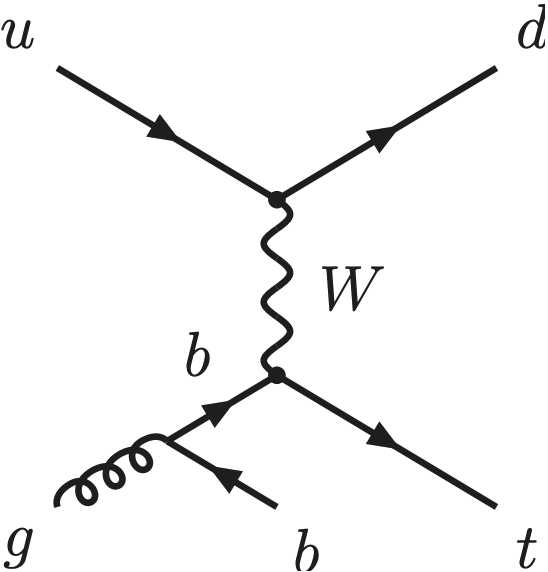
\includegraphics[width=\textwidth]{Chapter1/Single-top-tchannel-A}
         \caption{\tchannel}
         \label{fig:Chap1:top:singletop:tchannel_A}
     \end{subfigure}
     \hfill
     \begin{subfigure}[b]{0.3\textwidth}
                \centering
         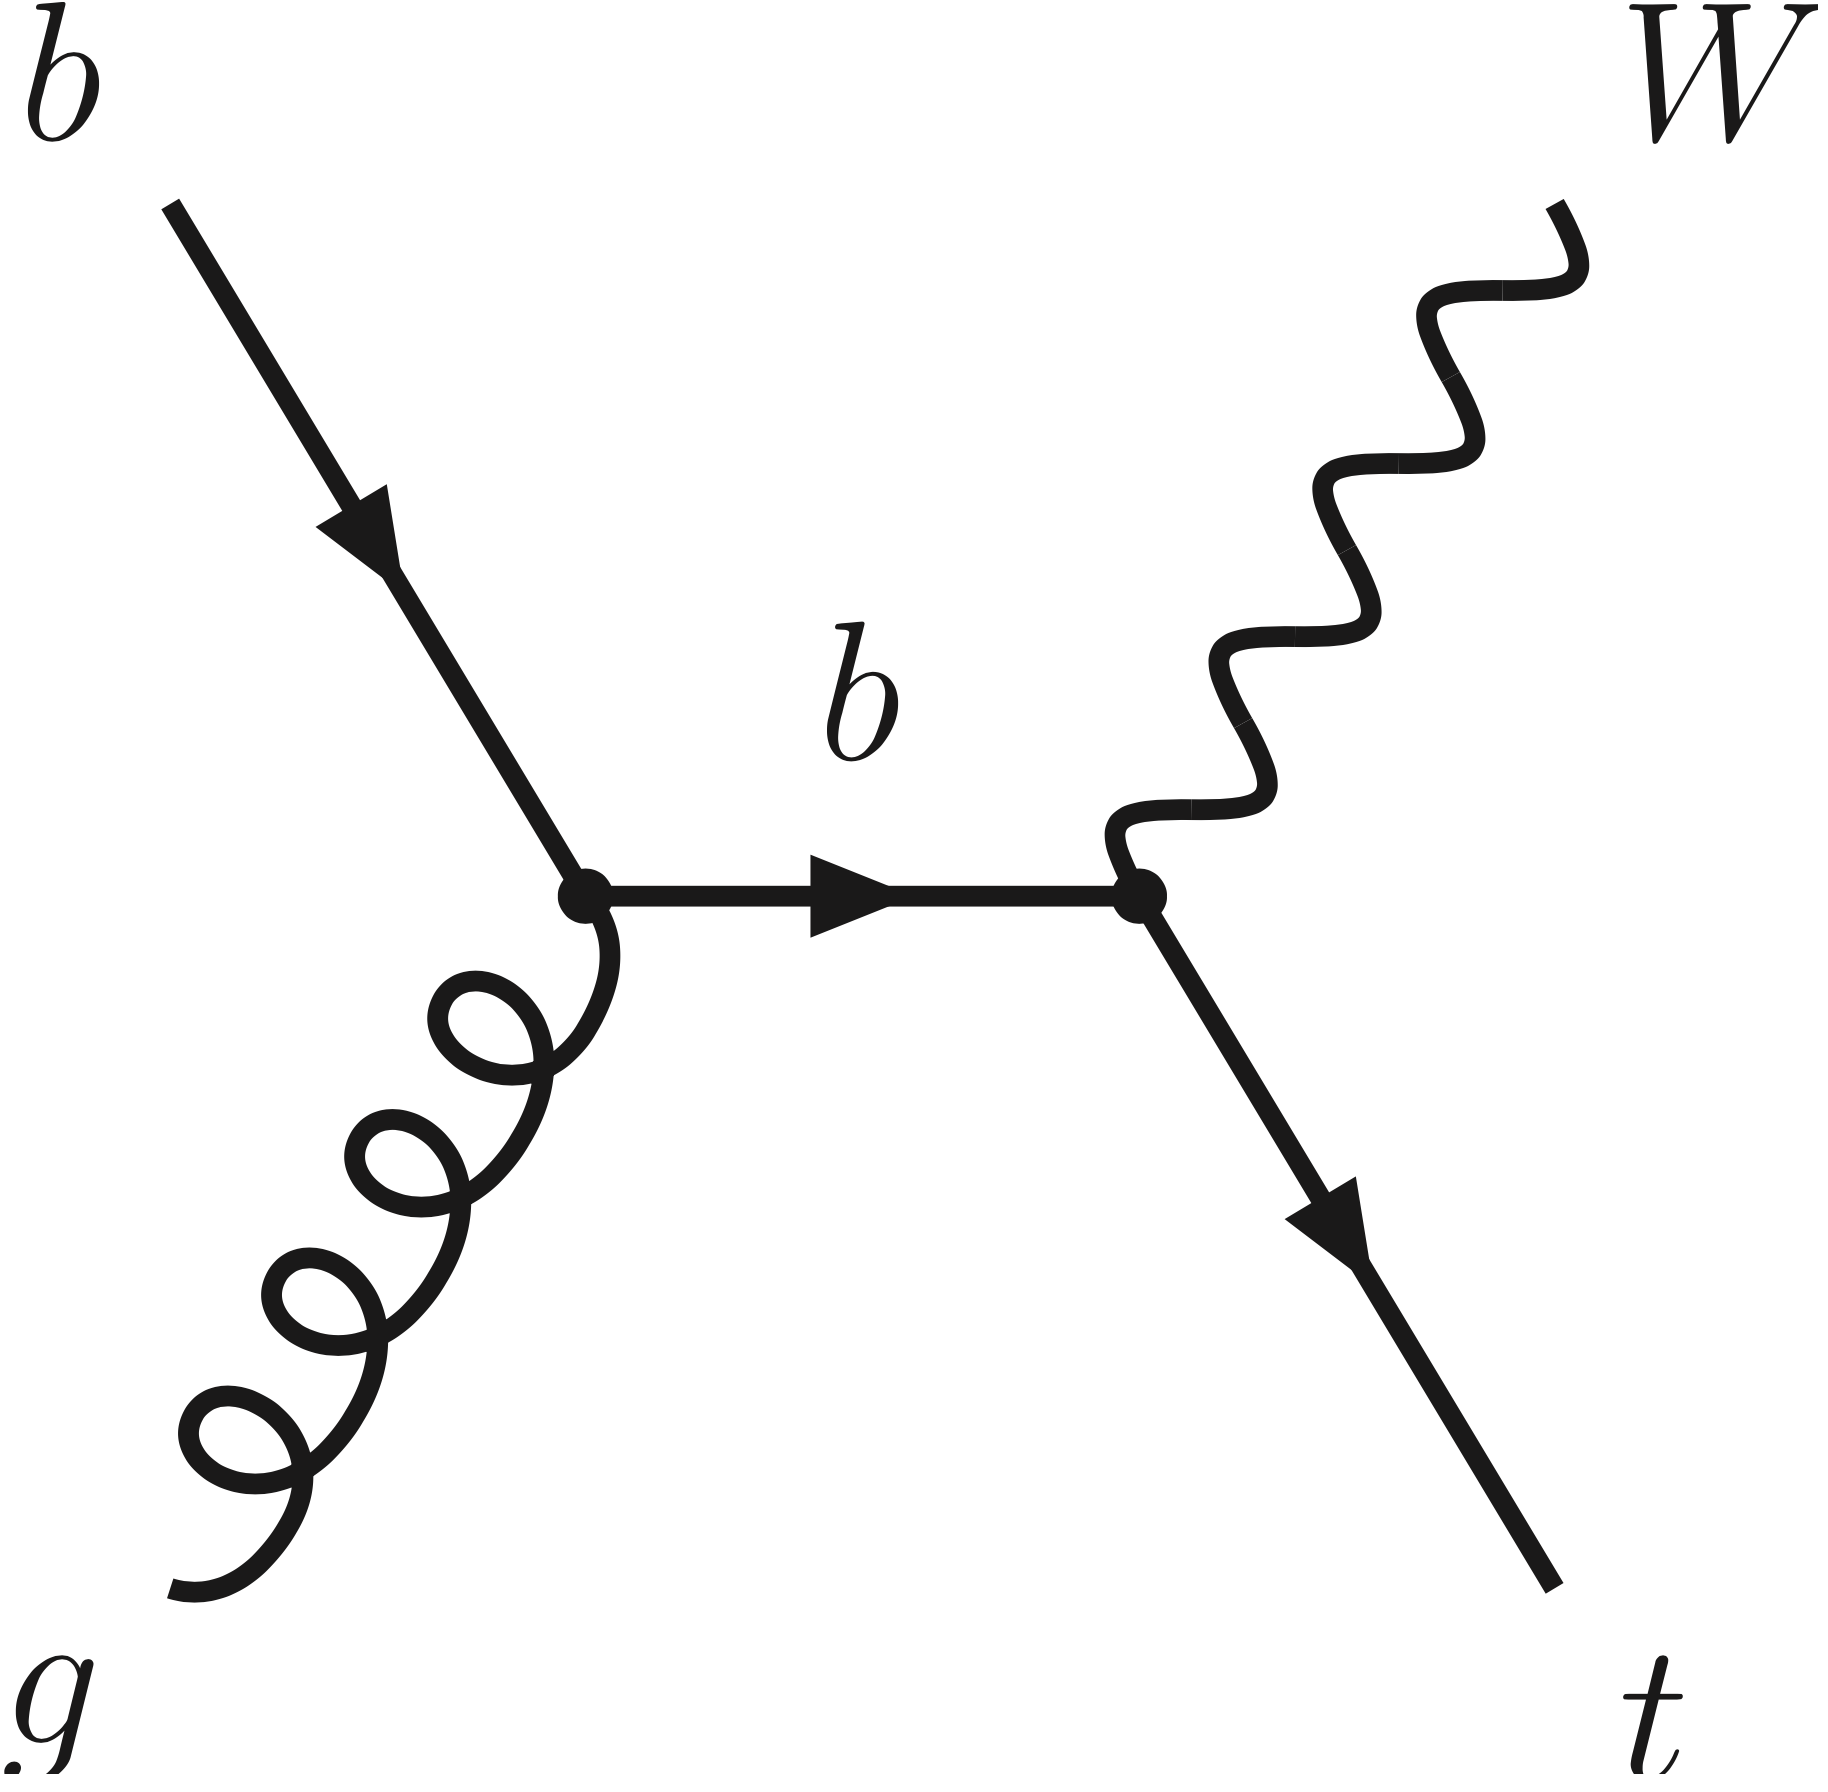
\includegraphics[width=\textwidth]{Chapter1/Single-top-Wt-B}
         \caption{\tW-channel}
         \label{fig:Chap1:top:singletop:tW_B}
     \end{subfigure}
     \hfill
     \begin{subfigure}[b]{0.3\textwidth}
         \centering
         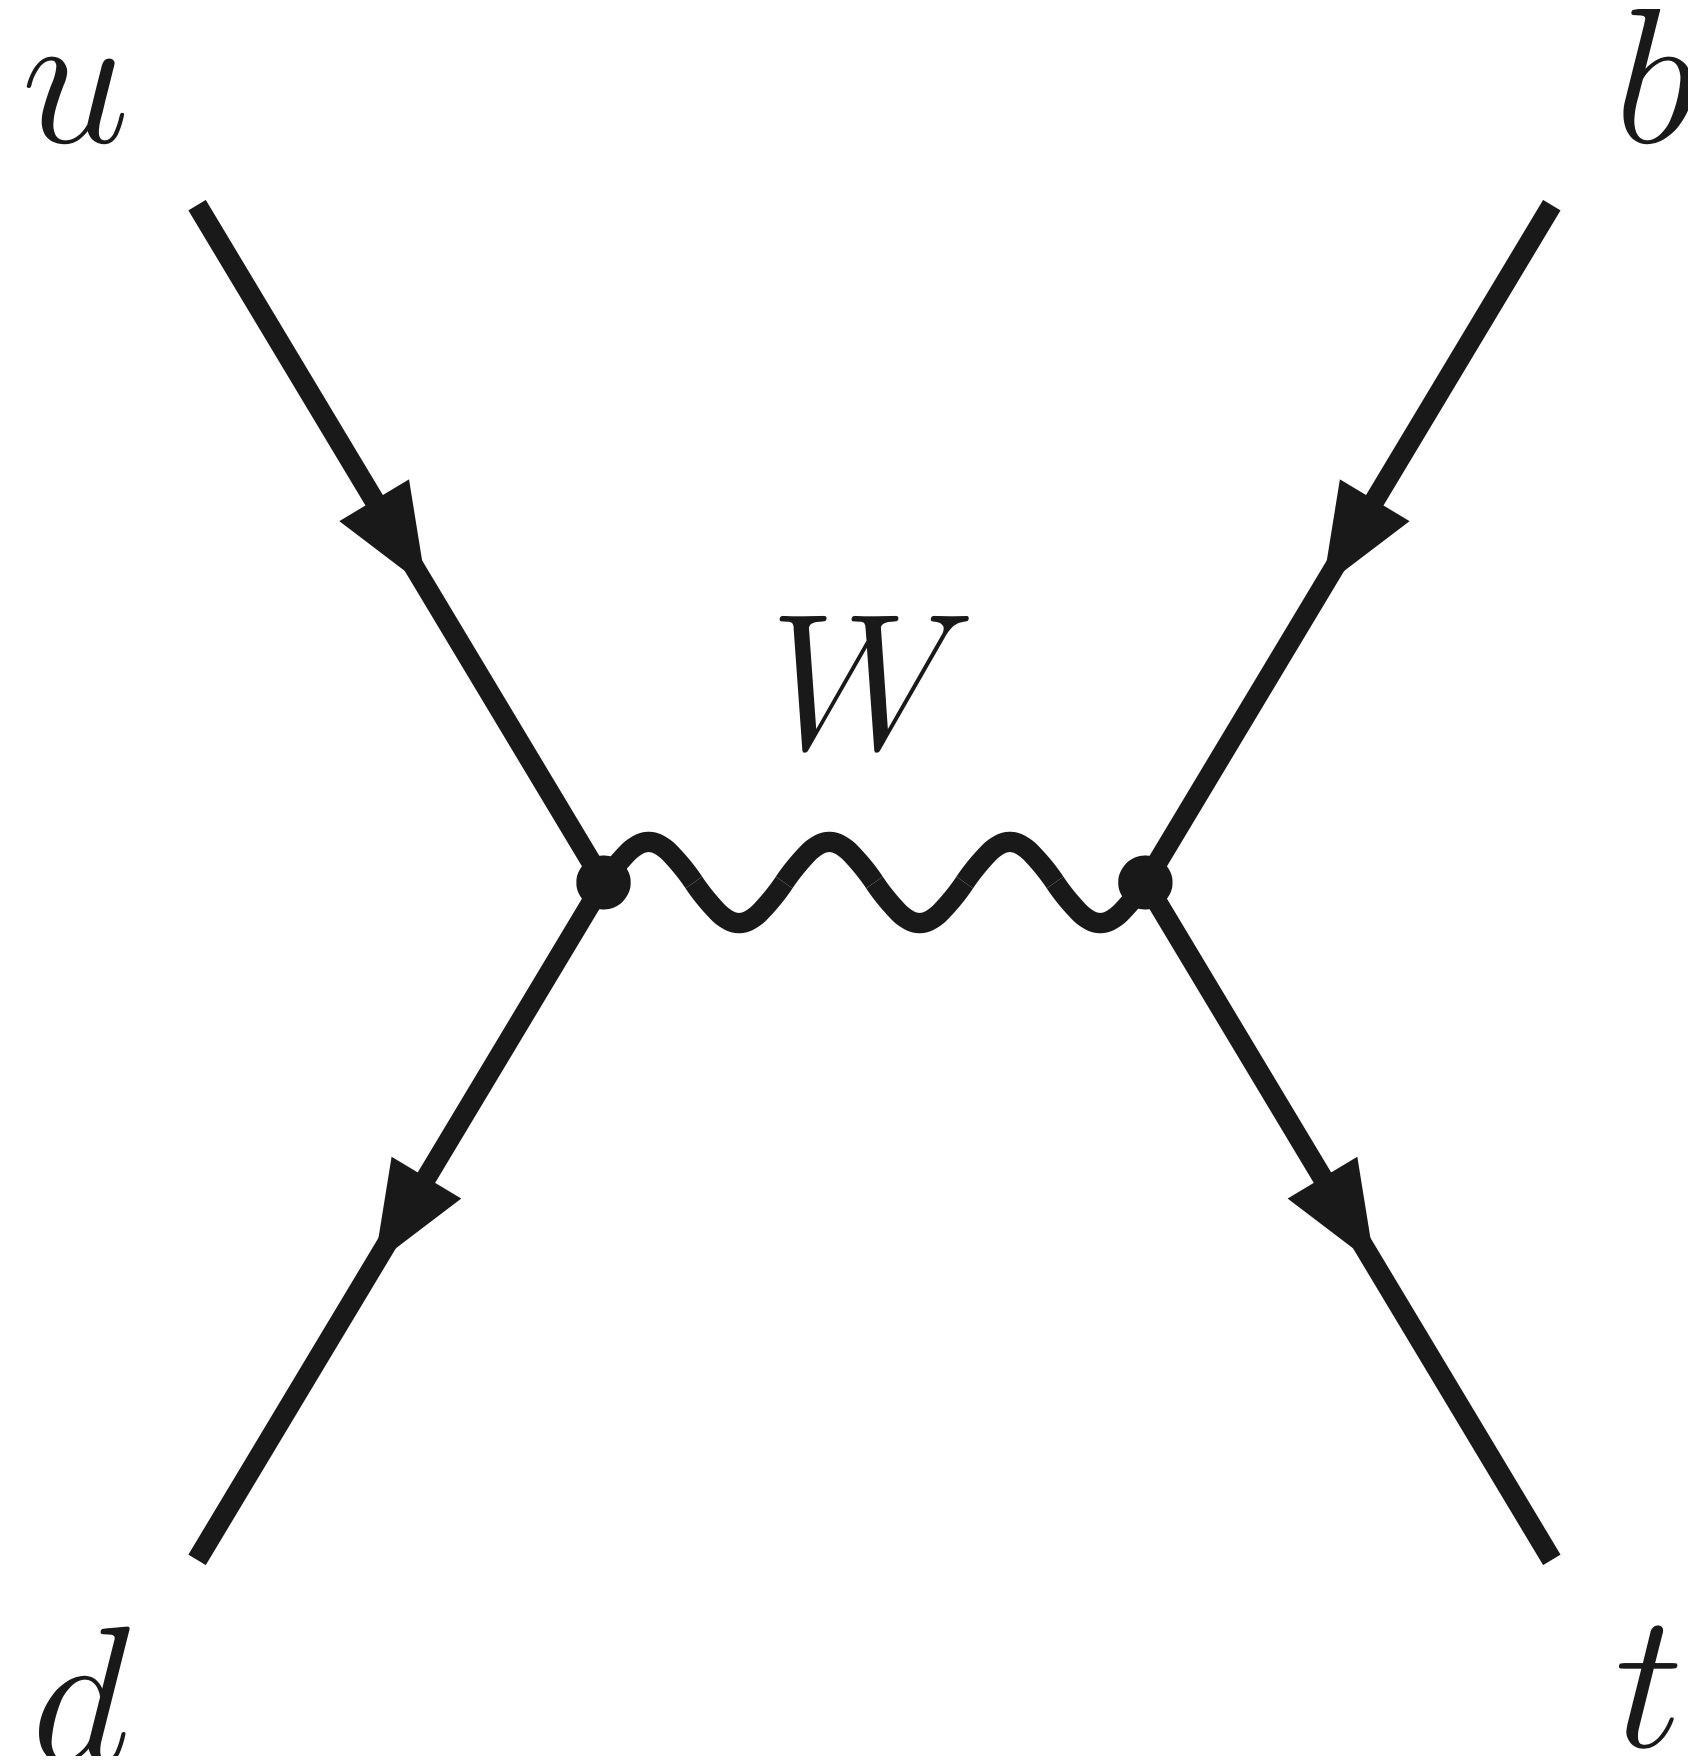
\includegraphics[width=\textwidth]{Chapter1/Single-top-schannel}
         \caption{\schannel}
         \label{fig:Chap1:top:singletop:schannel}
     \end{subfigure}
        \caption{Representative Feynman diagrams for the main three single-top-quark production channels at LO. 
        Observe that the \Pup and 
        \Pdown quarks could be substituted by \Pcharm and \Pstrange quarks.}
        \label{fig:Chap1:top:singletop:Main}
\end{figure}
\end{comment}




\begin{comment}
%%%     Single-top quark   :::  t-channel
\paragraph{\tchannel}\mbox{}\\
This production mode involves the scattering of a light quark and a gluon from the 
proton sea as shown in Figure~\ref{fig:Chap1:top:singletop:tchannel}.
Note that additional diagrams to those in Figure~\ref{fig:Chap1:top:singletop:tchannel} 
are obtained by either replacing the \Pup and \Pdown by a \Pcharm and \Pstrange
quarks or by switching the light quarks in the fermion line. The diagrams for antitop 
production are the charge conjugate of the ones presented. 

\begin{figure}
     \centering
     \begin{subfigure}[b]{0.3\textwidth}
         \centering
         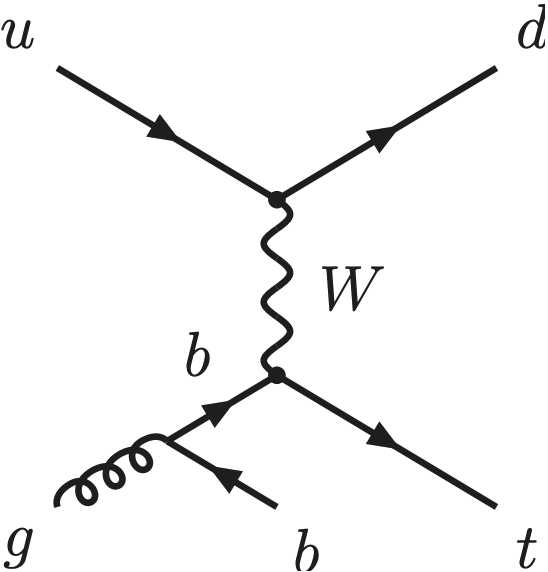
\includegraphics[width=\textwidth]{Chapter1/Single-top-tchannel-A}
         \caption{}
         \label{fig:Chap1:top:singletop:tchannel_A}
     \end{subfigure}
     \hfill
     \begin{subfigure}[b]{0.3\textwidth}
         \centering
         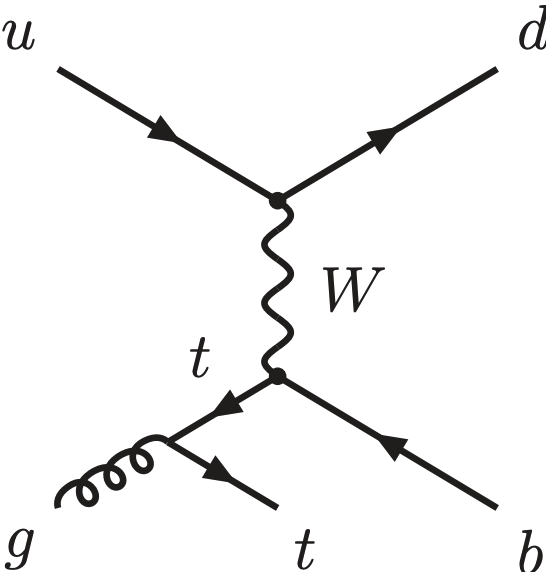
\includegraphics[width=\textwidth]{Chapter1/Single-top-tchannel-B}
         \caption{}
         \label{fig:Chap1:top:singletop:tchannel_B}
     \end{subfigure}
     \hfill
     \begin{subfigure}[b]{0.3\textwidth}
         \centering
         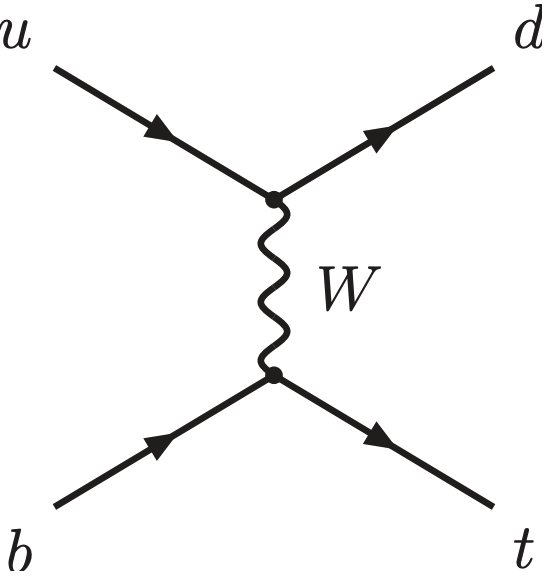
\includegraphics[width=\textwidth]{Chapter1/Single-top-tchannel-C}
         \caption{}
         \label{fig:Chap1:top:singletop:tchannel_C}
     \end{subfigure}
        \caption{Representative Feynman diagrams for the single-top-quark production in the \tchannel process. Observe that the \Pup and 
        \Pdown quarks could be substituted by \Pcharm and \Pstrange quarks.}
        \label{fig:Chap1:top:singletop:tchannel}
\end{figure}

The measurements cross-sections at $13$~TeV for single top quark ($\sigma_{\tchannel, \Ptop}$) 
and single-anti-top-qaurk ($\sigma_{\tchannel, \APtop}$) quarks in the \tchannel production are 
shown in Figure~\ref{fig:Chap1:top:singletop:tchannel_CrossSection}.
The theoretical calculation at next-to-leading order
(NLO) at $13$~TeV is $\sigma^{pred}_{\tchannel, \Ptop + \APtop }= 217.0^{+13.1}_{-11.1} \,\textrm{pb}$
\cite{CMS:2018lgn}. Due to the difference of valence quarks in the proton, the ratio 
between $\sigma^{pred}_{\tchannel, \Ptop}$ and $\sigma^{pred}_{\tchannel, \APtop}$ is 1.56. These numbers 
are obtained using \HATHOR[2.1]~\cite{Kant:2014oha, Aliev:2010zk} and a \mtop of $172.5$~GeV.
%\begin{align*}
	%\sigma_{\tchannel, \Ptop} &= 136^{+4.1}_{-2.9} (\textrm{scale}) \pm 3.5(\textrm{PDF}+\alpha_{s})\,\textrm{pb,} \\
	%\sigma_{\tchannel, \APtop} &= 81.0^{+2.5}_{-1.7} (\textrm{scale}) \pm 3.2(\textrm{PDF}+\alpha_{s})\,\textrm{pb,} \\
	%\sigma_{\tchannel, \Ptop + \APtop} &= 217^{+6.6}_{-4.6} (\textrm{scale}) \pm 6.5(\textrm{PDF}+\alpha_{s})\,\textrm{pb.}
	%\sigma_{\tchannel, \Ptop} &= 136^{+7.6}_{-6.4}\,\textrm{pb,} \\
	%\sigma_{\tchannel, \APtop} &= 81.0^{+5.7}_{-4.9} \,\textrm{pb,} \\
	%\sigma_{\tchannel, \Ptop + \APtop} &= 217.0^{+13.1}_{-11.1} \,\textrm{pb.} \\
%\end{align*} % CMS Experimental results for these cross-sections in: https://arxiv.org/pdf/1901.05247.pdf


\begin{figure}[h]
    \centering
    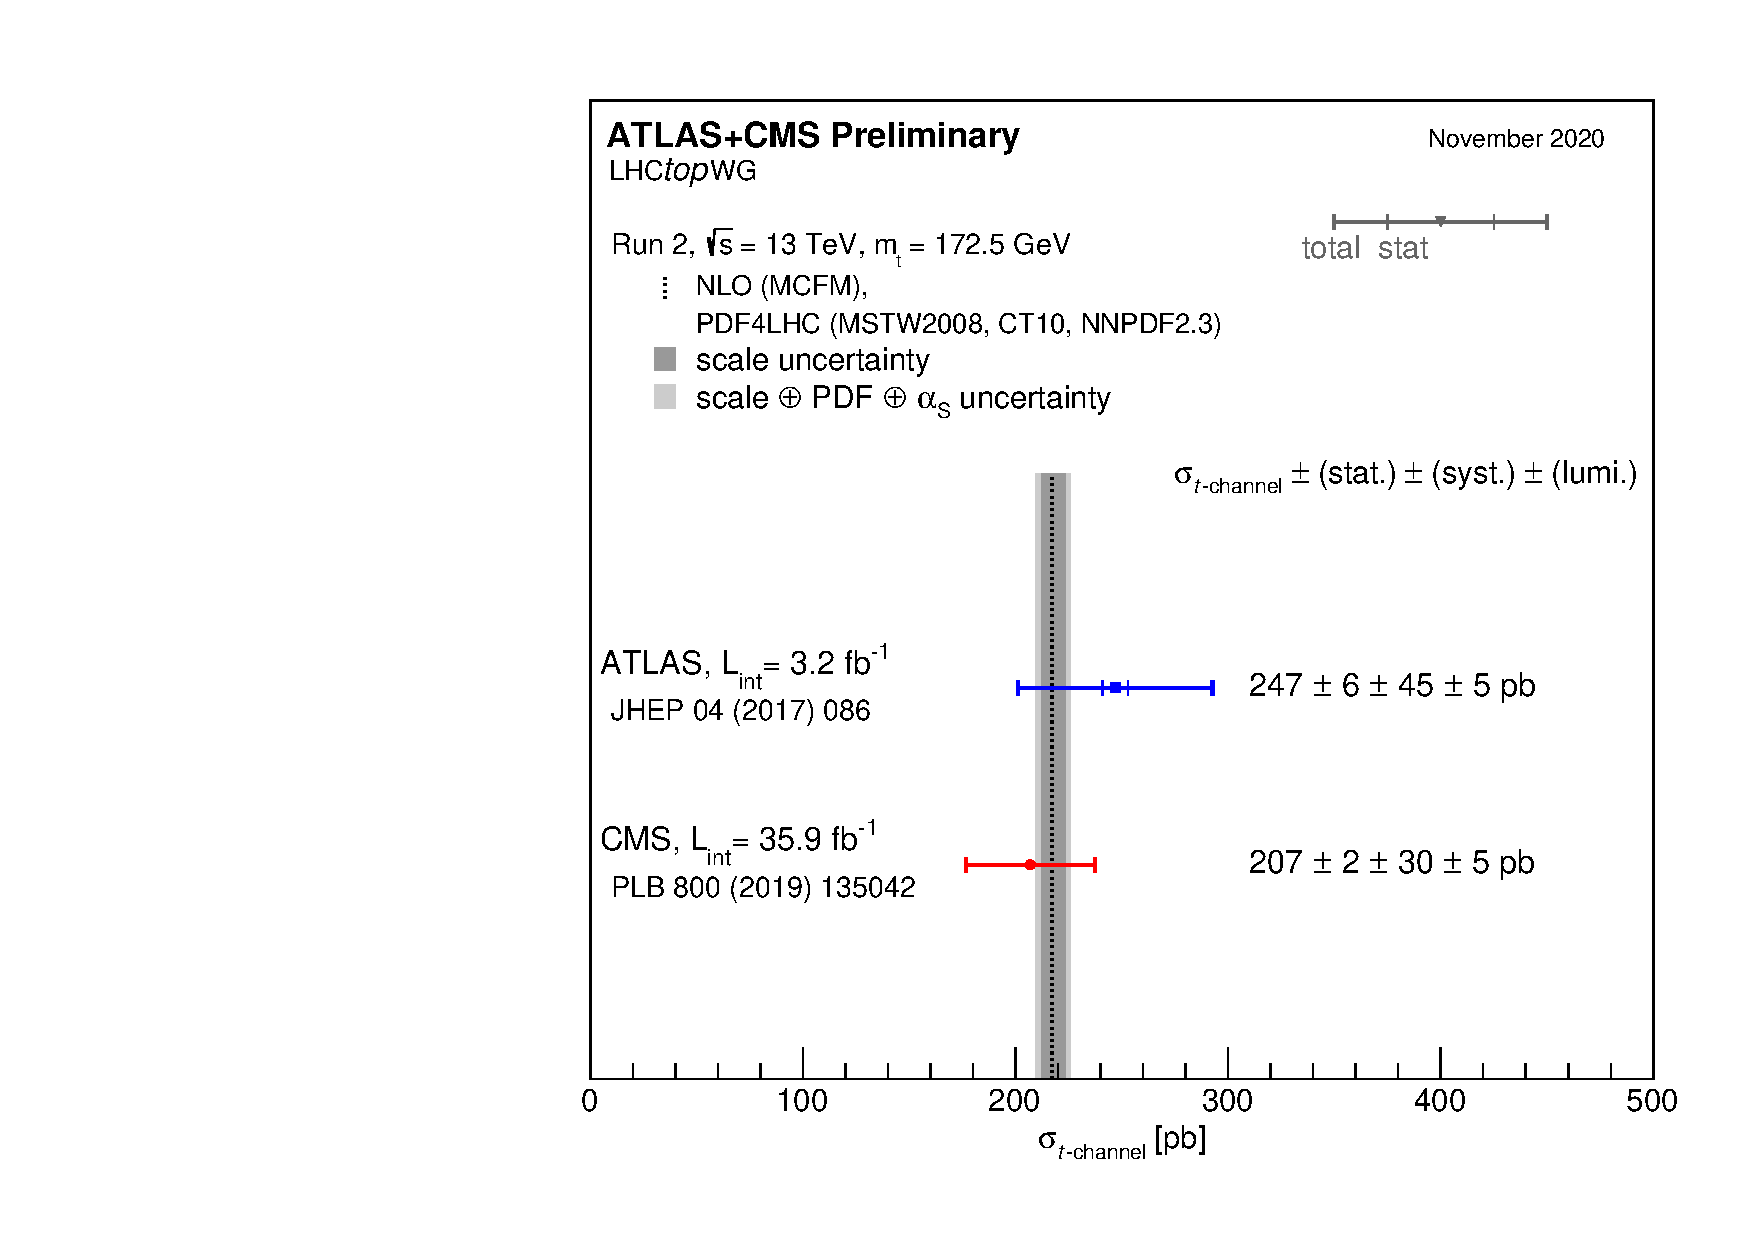
\includegraphics[width = 0.75\textwidth]{Chapter1/singletop_tchan_xsec_13_lhc_nov20}
    \caption{Summary of the ATLAS and CMS measurements of the single-top-quark production cross-sections in the \tchannel at $13$~TeV. The measurements are compared to NLO calculations~\cite{ATLAS:2022uqj}.}
    \label{fig:Chap1:top:singletop:tchannel_CrossSection}
\end{figure}


The dominant process in the SM is the one in diagram \ref{fig:Chap1:top:singletop:tchannel_A}, while 
the one in \ref{fig:Chap1:top:singletop:tchannel_B} is included in order to form a gauge invariant set 
but its contribution is not very significative since for the gluon is easier to decay to $\Pbottom\APbottom$ 
pair than to a $\Ptop\APtop$ pair. These two $2 \rightarrow 3$ production modes are known 
as 4 Flavour Scheme (FS) because the proton is considered to be composed
by four quark flavours (\Pup, \Pdown, \Pcharm and \Pstrange). It is characterised by having a \Pbottom 
quark in the final state. This final-state \Pbottom-quark is sometimes referred to as second\footnote{The 
first would be the one from the top quark decay.}.% \Pbottom and it 
%has a transverse momentum (\pT) distribution peaking around 2 or 3 GeV as can be seen 
%in Figure~\ref{fig:Chap1:top:singletop:tchannel:ptVSeta}. This is the reason why the final \Pbottom quark 
%from the gluon splitting frequently goes undetected, because it does not pass the \pT threshold of the detector. 
%This is why, at detector level, whenever only jet is identified as originated from a \Pbottom quark, it is assumed to be
%the \Pbottom from the top-quark decay. This particularity becomes more important in  Chapter \ref{chap:Analysis_tH},
%where the number of detected \btagged jets is a relevant variable for the definition of the preselection region.


The $2 \rightarrow 2$ process in \ref{fig:Chap1:top:singletop:tchannel_C} is known as 
5FS because the proton has 
four flavours of quarks and since the process has a \Pbottom quark in the initial state, there are the five flavours.
The simulations for the 4FS and 5FS diagrams are produced separately and
merged afterwards. When adding the two contributions, some double-counting may appear due to the overlap in the phase space so one has to be careful. The naming 4FS and 5FS is later used again for the associated \tH production.


%%%     Single-top quark   :::  s-channel
\paragraph{\schannel}\mbox{}\\
The \schannel process is the one with less impact among single-top-quark production channels.  
It is depicted in Figure~\ref{fig:Chap1:top:singletop:schannel}. 
This production mode is also referred to as the quark-antiquark annihilation or $W^{*}$ process  and it is very similar
to the Drell-Yann. 

According to the LHC cross-section group, at $\CM=13$~TeV, the combined 
cross-section for the single top and single anti-top production in the \schannel 
is $\sigma^{pred}_{\schannel, \Ptop + \APtop} = 10.32^{+0.56}_{-0.61} \,\textrm{pb}$ 
\cite{Kant:2014oha}.
%\begin{align*}
%	\sigma_{\schannel, \Ptop} &= 6.35^{+0.18}_{-0.15} (\textrm{scale}) \pm 0.9(\textrm{PDF}+\alpha_{s})\,\textrm{pb,} \\
%	\sigma_{\schannel, \APtop} &= 3.97^{+0.11}_{-0.09} (\textrm{scale}) \pm 0.15(\textrm{PDF}+\alpha_{s})\,\textrm{pb,} \\
%	\sigma_{\schannel, \Ptop + \APtop} &= 10.32^{+0.29}_{-0.34} (\textrm{scale}) \pm 0.27(\textrm{PDF}+\alpha_{s})\,\textrm{pb.}
%	\sigma_{\schannel, \Ptop + \APtop} &= 10.32^{+0.56}_{-0.61} \,\textrm{pb.}
%\end{align*} % Source: https://twiki.cern.ch/twiki/bin/view/LHCPhysics/SingleTopRefXsec#Single_top_s_channel_cross_secti

%\begin{figure}
%    \centering
%    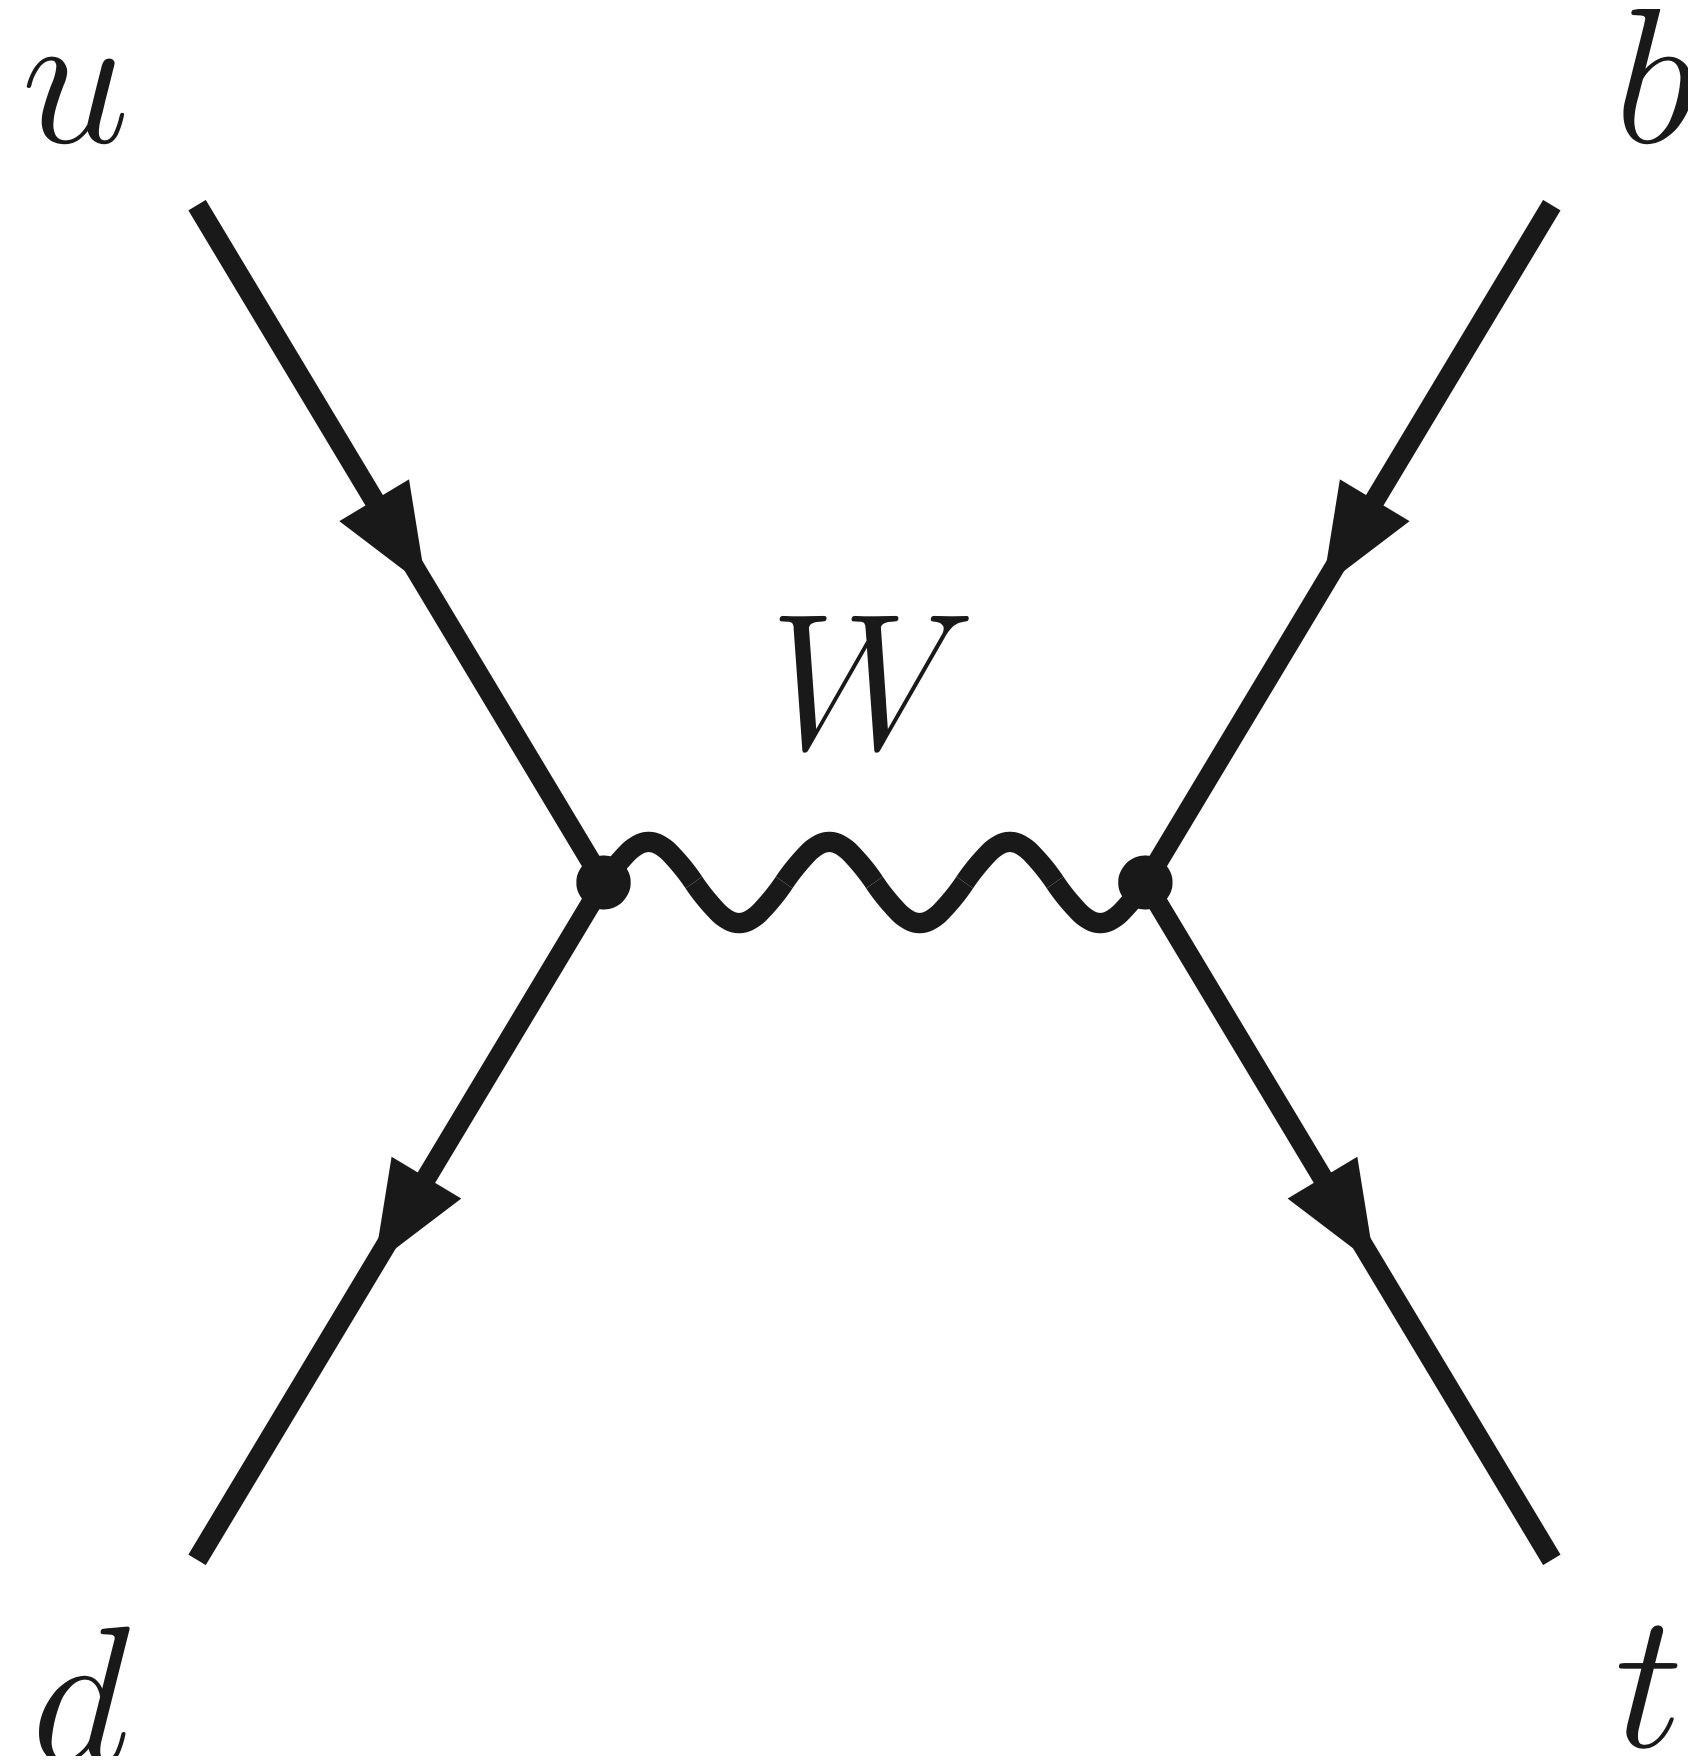
\includegraphics[width = 0.34\textwidth]{Chapter1/Single-top-schannel}
%    \caption{Representative Feynman diagram for the single-top-quark production in the \schannel.}
%    \label{fig:Chap1:top:singletop:schannel}
%\end{figure}

\begin{figure}
     \centering
     \begin{subfigure}[b]{0.3\textwidth}
         \centering
         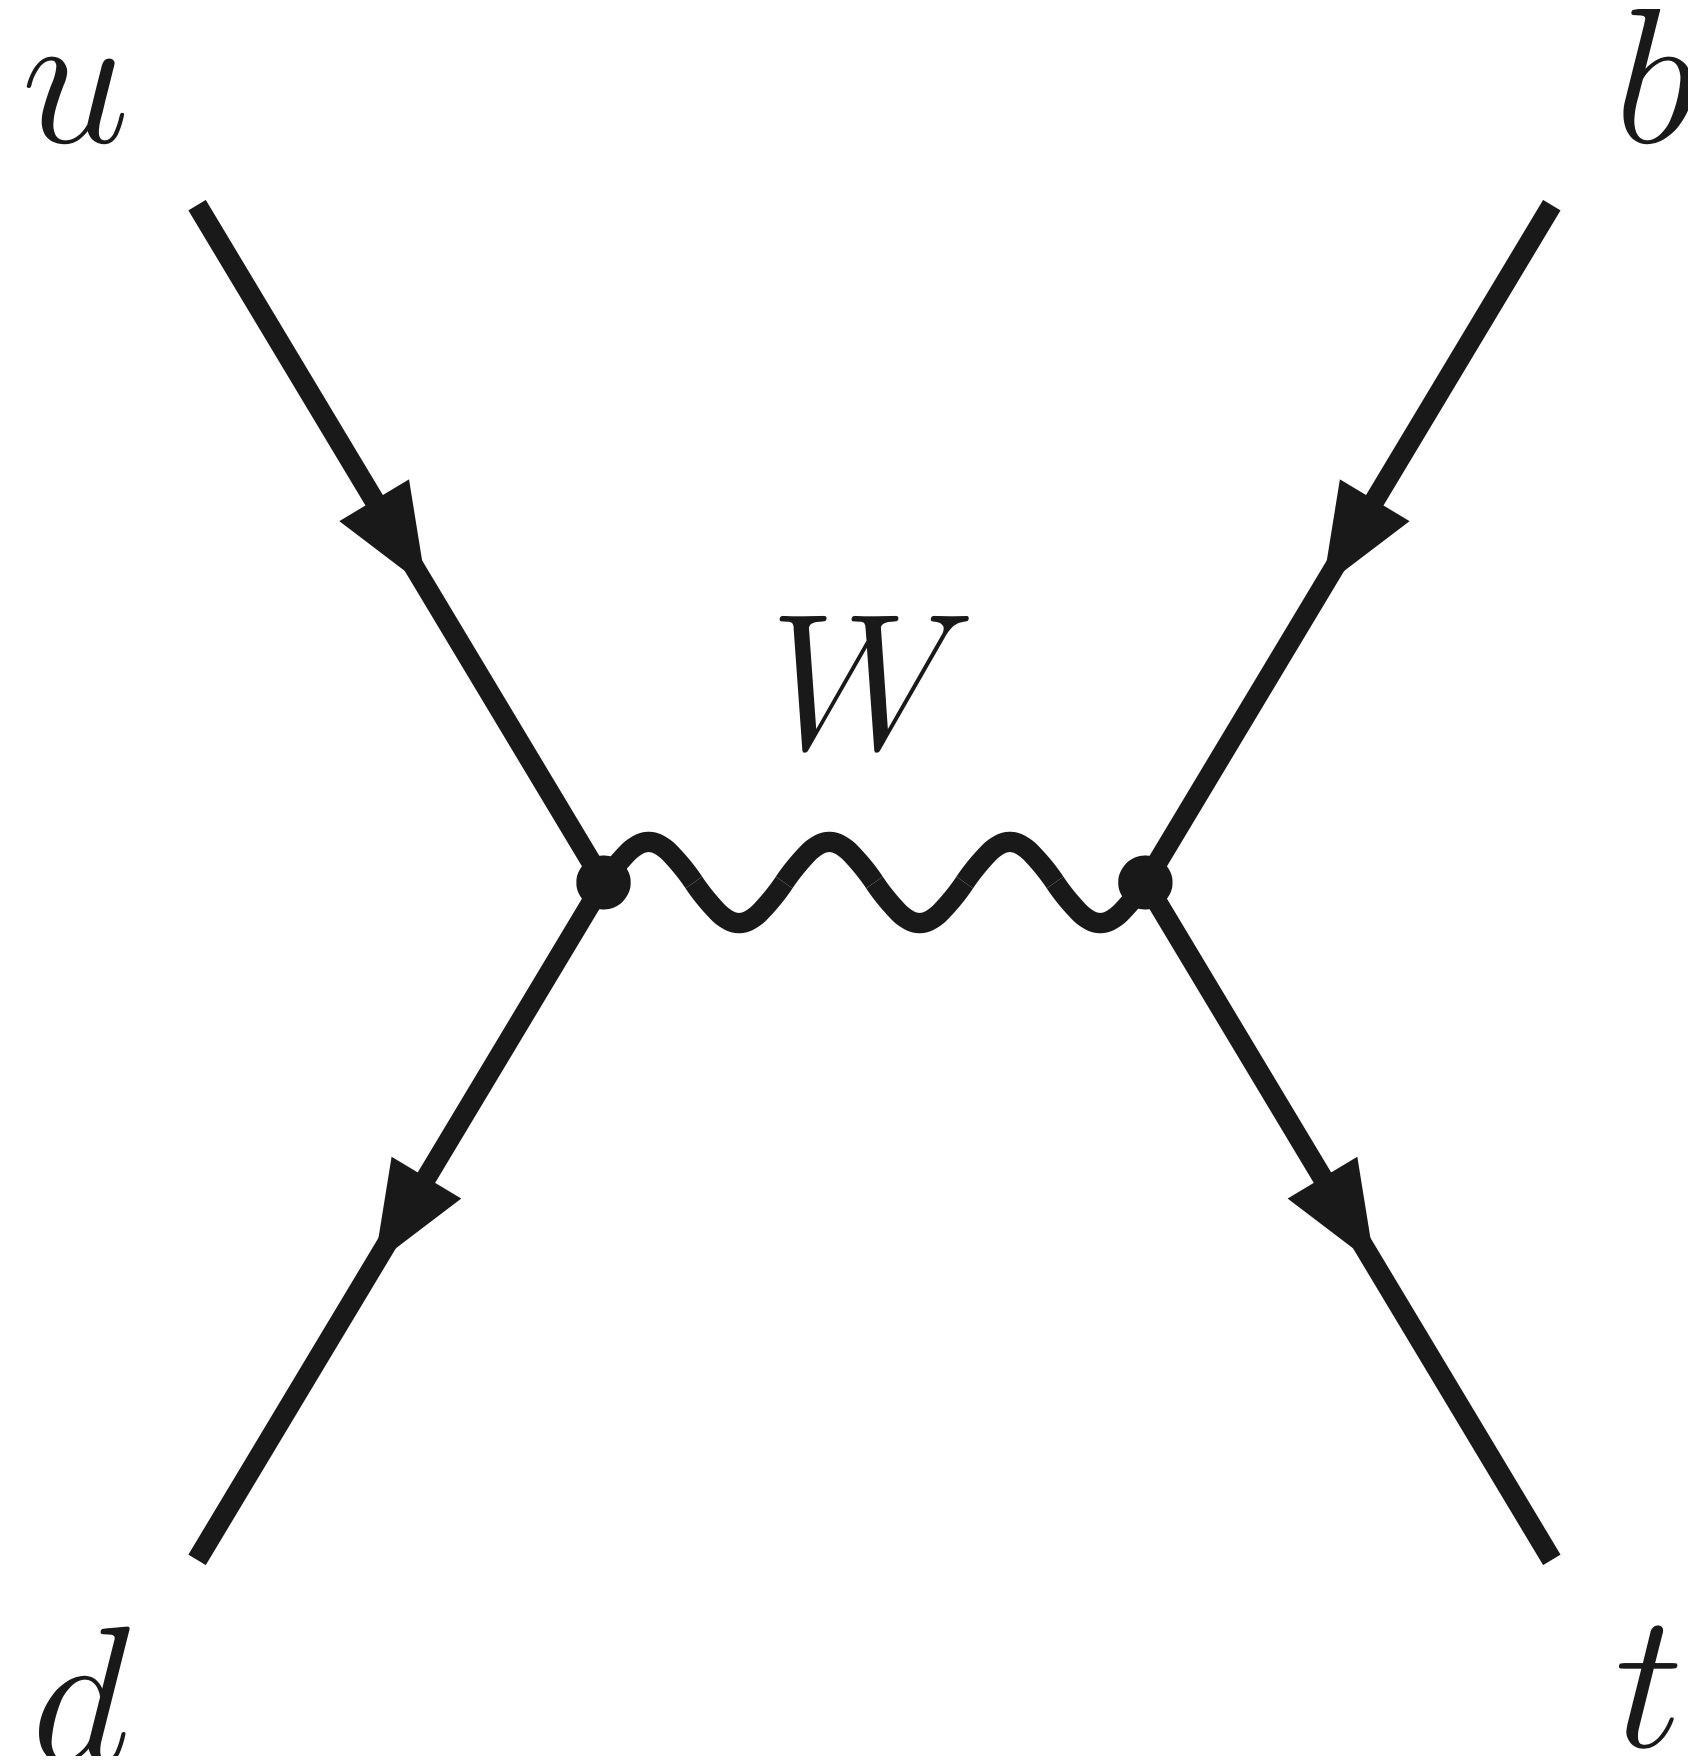
\includegraphics[width=\textwidth]{Chapter1/Single-top-schannel}
         \caption{}
         \label{fig:Chap1:top:singletop:schannel}
     \end{subfigure}
     \begin{subfigure}[b]{0.3\textwidth}
         \centering
         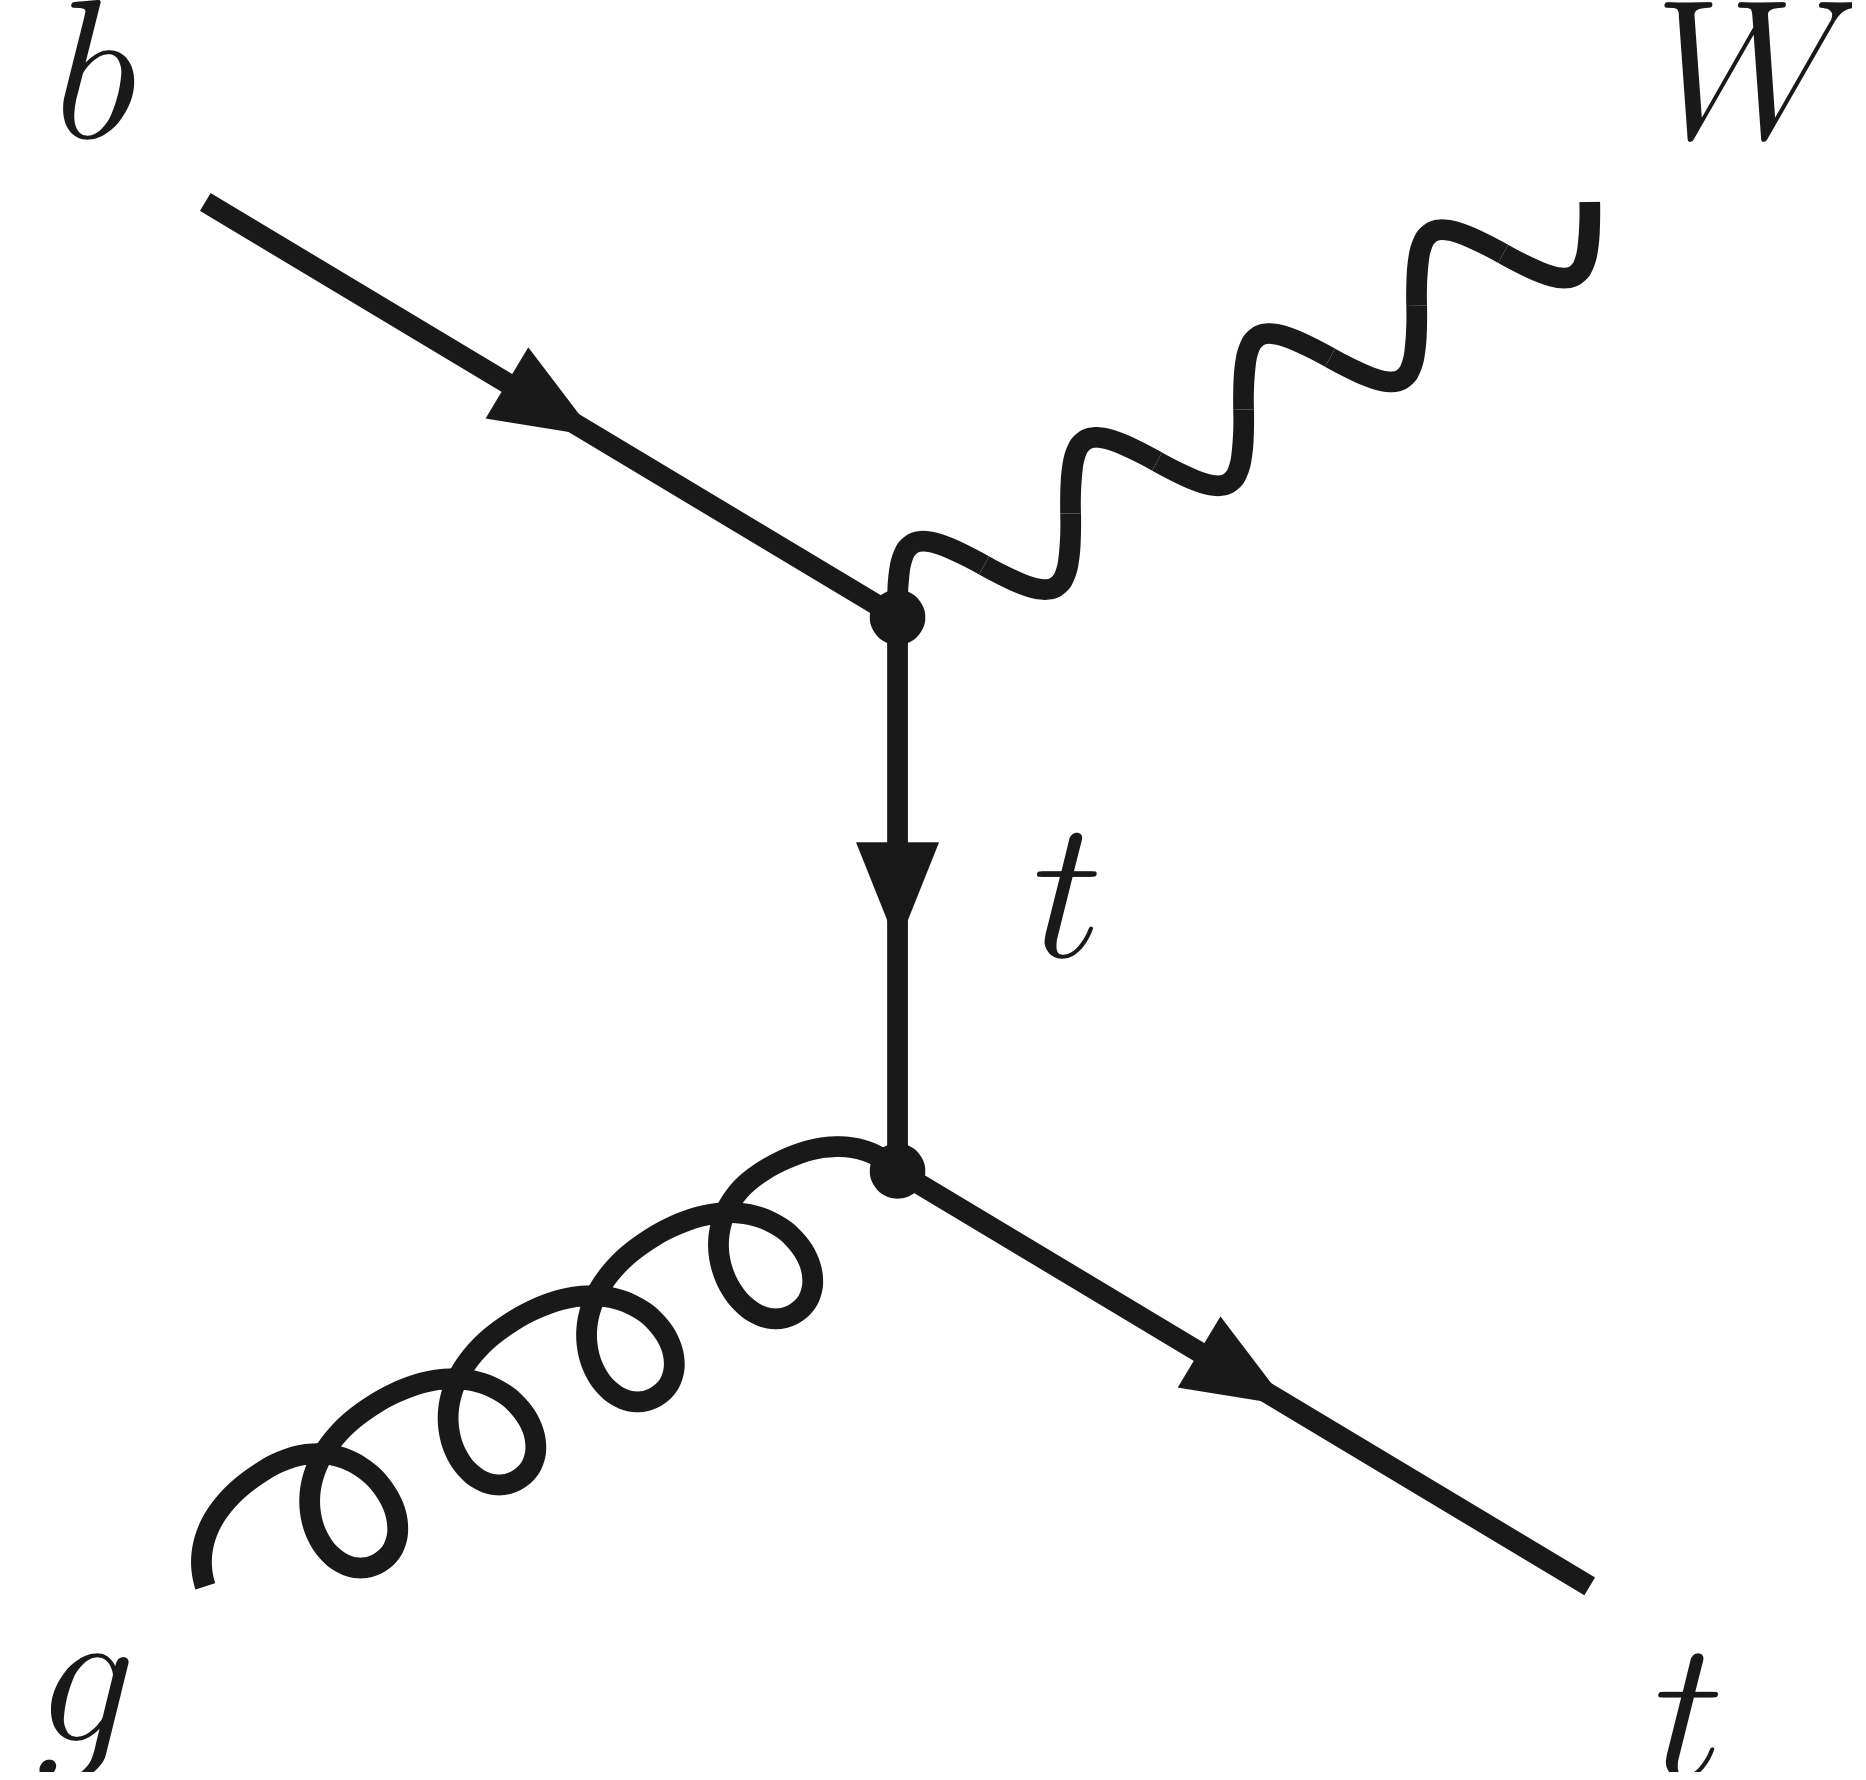
\includegraphics[width=\textwidth]{Chapter1/Single-top-Wt-A}
         \caption{}
         \label{fig:Chap1:top:singletop:tW_A}
     \end{subfigure}
     \begin{subfigure}[b]{0.3\textwidth}
         \centering
         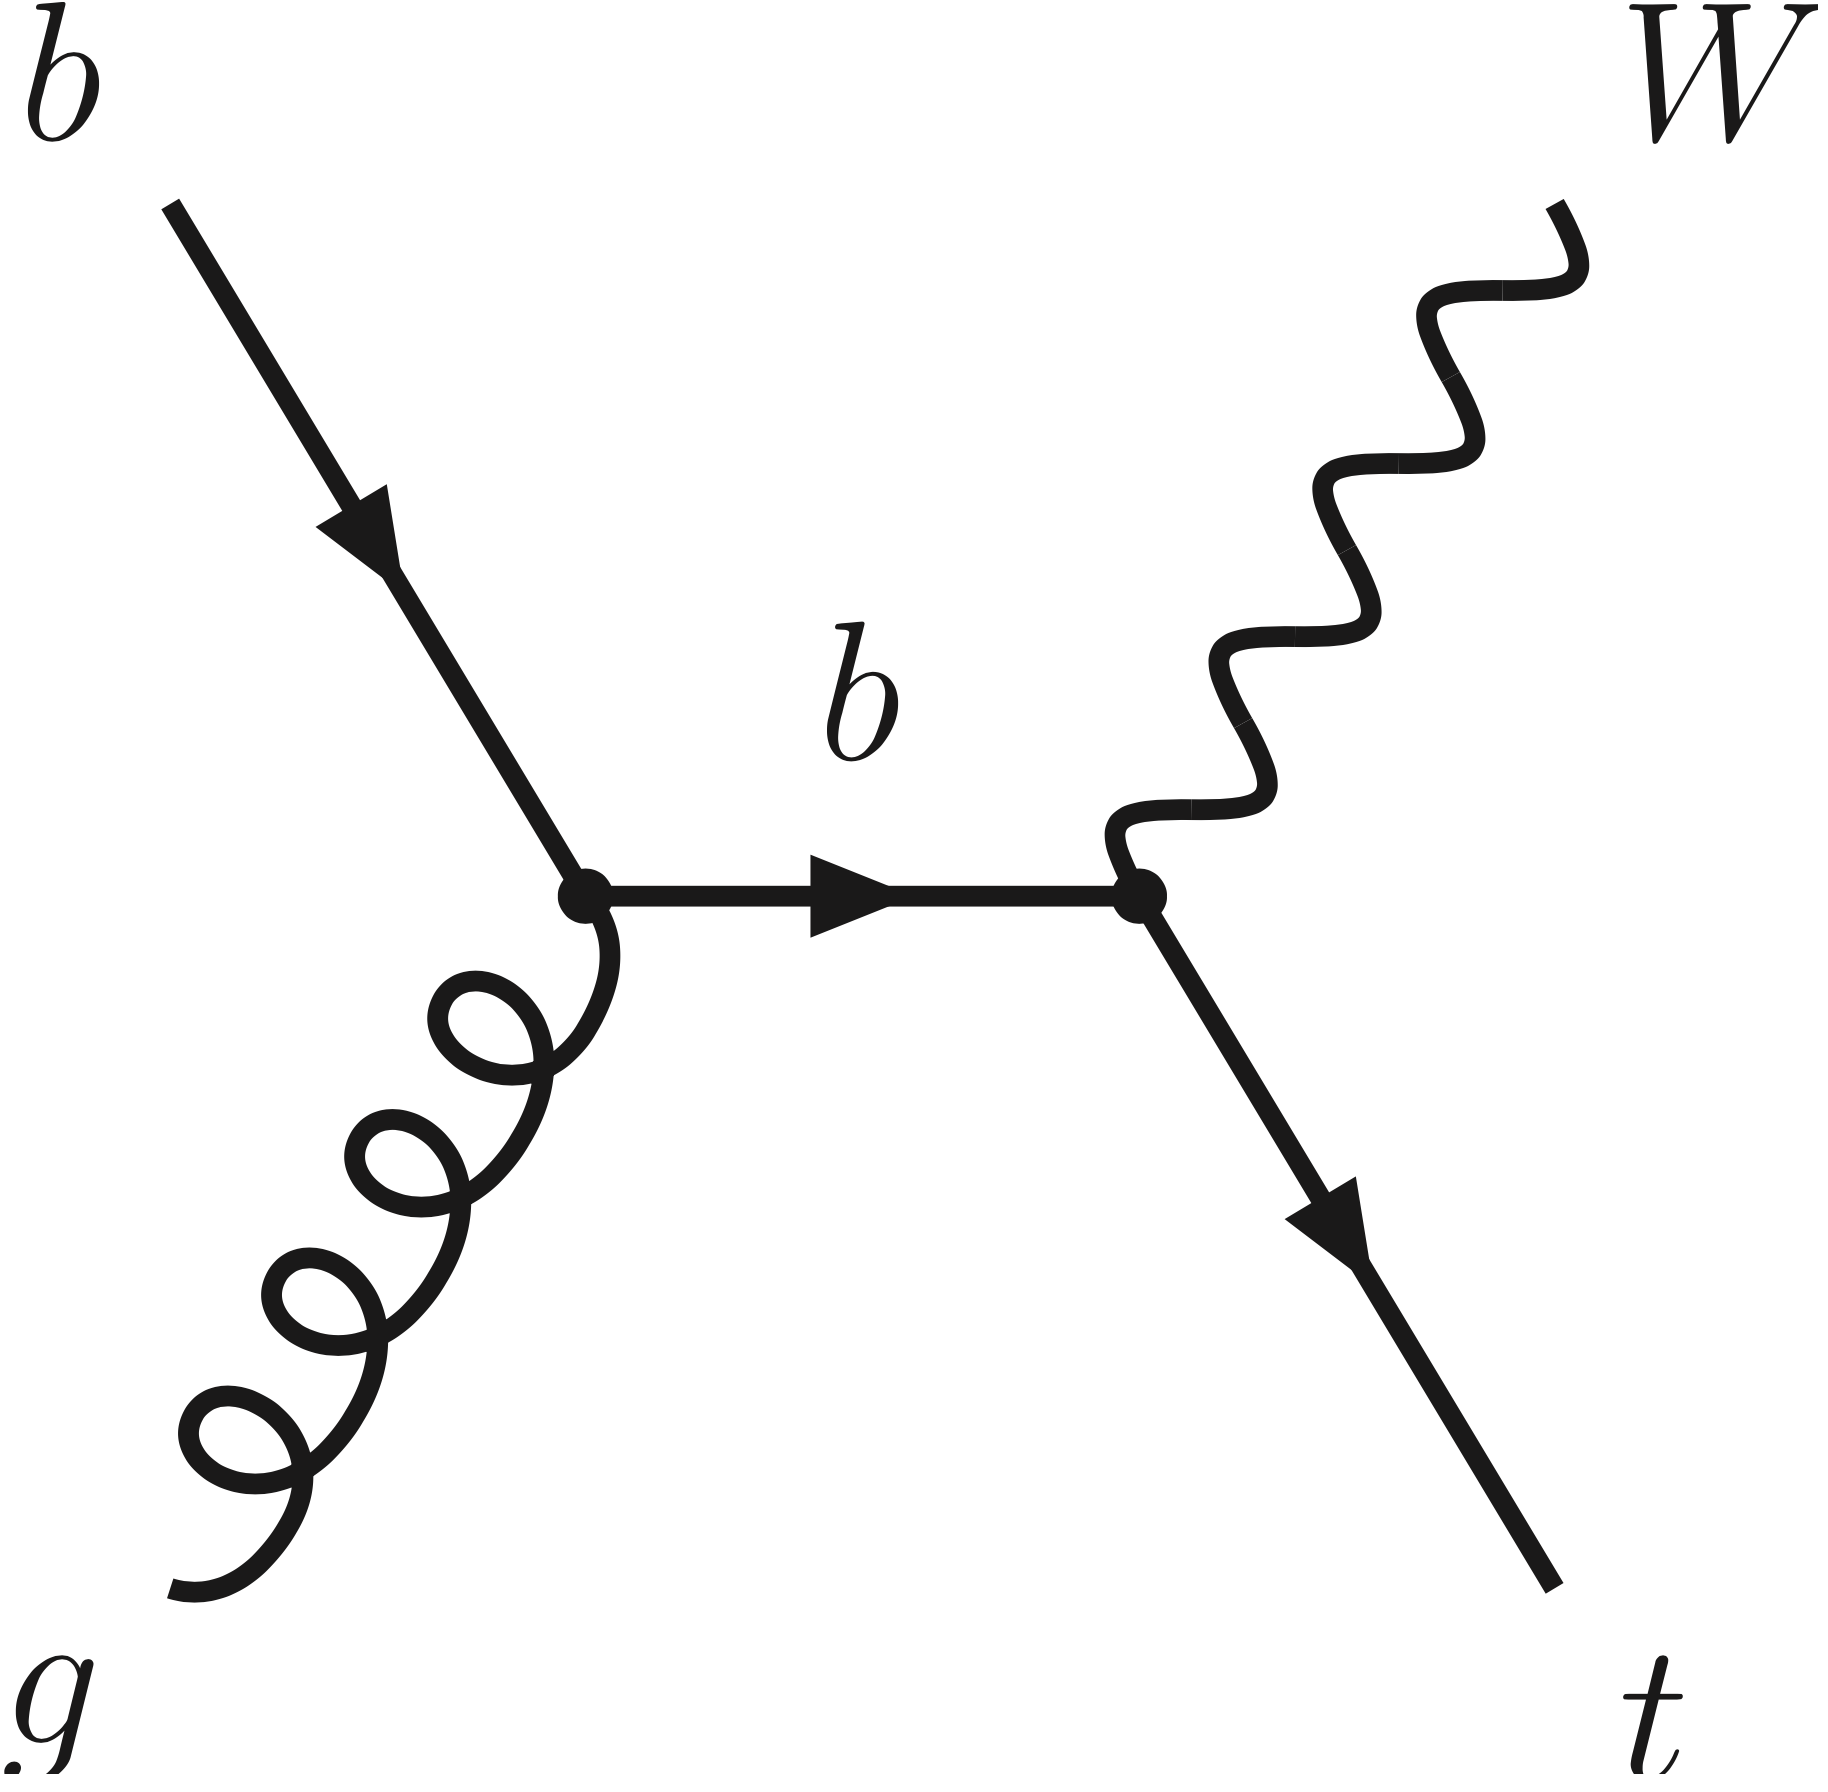
\includegraphics[width=\textwidth]{Chapter1/Single-top-Wt-B}
         \caption{}
         \label{fig:Chap1:top:singletop:tW_B}
     \end{subfigure}
        \caption{Representative Feynman diagrams for the single-top-quark production in (a) the \schannel
        and with (b, c) an associtared \PW boson. While the first one is not observed, the $\Ptop\PW$ is one the backgrounds
        in the \tHq analysis.}
        \label{fig:Chap1:top:singletop:SchannelAndAssocited}
\end{figure}


Although while at the LHC only an evidence\footnote{The threshold for "evidence" corresponds to 
p-value=0.003 (three standard-deviations) while the standard for "discovery" is 
p-value=0.0000003 (five standard-deviations). \pablo{Review this p-values}}
of the \schannel production has been found~\cite{ATLAS:2022wfk}, for Tevatron it was a
a significant part of the total single-top cross-section~\cite{Cremonesi:2014dma}. 
% Table 4 of https://citeseerx.ist.psu.edu/viewdoc/download?doi=10.1.1.205.6486&rep=rep1&type=pdf


%%%     Single-top quark   :::  associated Wt-channel
\paragraph{Associated $\Ptop\PW$}\mbox{}\\
%\begin{minipage}[t]{0.5\linewidth}
Finally, the associated production of a single top quark with a \PW boson 
(sometimes referred to as $\Ptop\PW$-channel) is represented by two the Feynman 
diagrams in Figures \ref{fig:Chap1:top:singletop:tW_A} and \ref{fig:Chap1:top:singletop:tW_B}.
To these two diagrams, the charge conjugate processes could be added to 
complete the $\Ptop\PW$ mechanisms. 
The predicted cross-section for the associated $\Ptop\PW$ is
$\sigma^{pred}_{tW, \Ptop + \APtop} = 71.7 \pm 5.2 \,\textrm{pb}$. This and 
all $\sigma$ in this section are calculated for a top mass of $\mtop = 172.5$~GeV.

Cross-section measurements for the associated $\Ptop\PW$ production 
performed by ATLAS and CMS at $13$~TeV have found
 $\sigma_{tW} = 94^{+38}_{-32} \,\textrm{pb}$~\cite{ATLAS:2016ofl}
and $\sigma_{tW} = 79.2 \pm 8.9\,\textrm{pb}$~\cite{CMS:2022xey} respectively. 
Both results are compatible with the NLO +NNLL prediction.
%\begin{equation*}
	%\sigma_{tW, \Ptop + \APtop} &= 71.7 \pm 1.80 (\textrm{scale}) \pm 3.40(\textrm{PDF}+\alpha_{s})\,\textrm{pb.}
%	\sigma_{tW, \Ptop + \APtop} = 71.7 \pm 5.2 \,\textrm{pb.}
%\end{equation*}

%and NLO in QCD with \HATHOR v.2.1. The PDF and $\alpha_{s}$ uncertainties are calculated
%using the PDF4LHC prescription~\cite{Butterworth:2015oua} with the 
%MSTW2008 68\% CL NLO~\cite{Martin:2009iq, Martin:2009bu}, CT10 NLO~\cite{Lai:2010vv} 
%and NNPDF2.3~\cite{Ball:2013hta} PDF sets, added in quadrature to the scale uncertainty.
%The measurements for the associated $\Ptop\PW$ are shown in Figure~\ref{fig:Chap1:top:singletop:tW_CrossSection}.
%The associated $\Ptop\PW$ production is an important background in the studies of the Higgs boson.
%\end{minipage} \hfill
%\begin{minipage}[t]{0.4\textwidth}
%\setbox0=\hbox{T} % tallest letter of the first line of other minipage
%\vskip-\ht0
%\begin{figure}
	%\begin{wrapfigure}{r}{0.45\textwidth}
%	    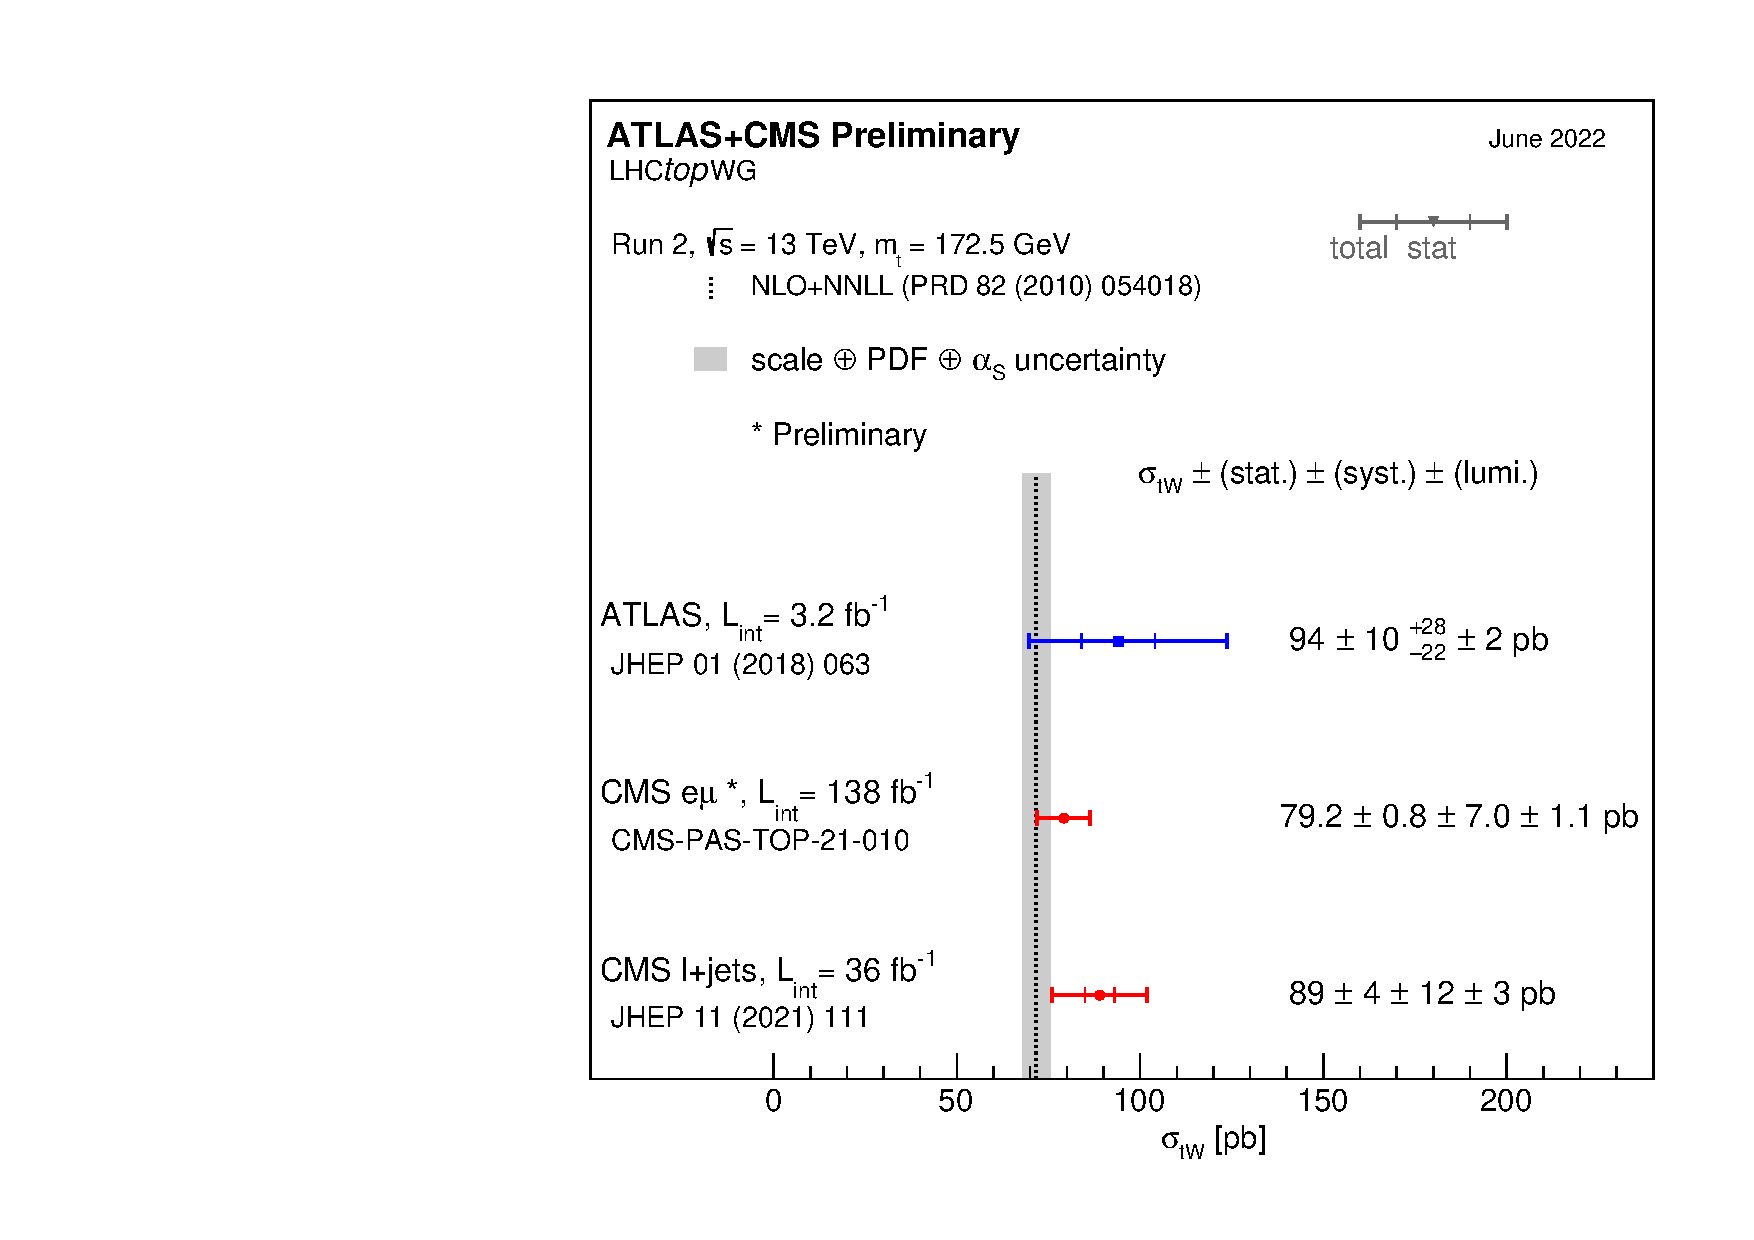
\includegraphics[width = 0.95\linewidth]{Chapter1/singletop_tW13_jun22}
% 	   \captionof{figure}{Cross-section measurements for the associated $\Ptop\PW$ production boson 
%	   performed by ATLAS and CMS at $13$~TeV, and combined result compared 
%	   with the NLO + next-to-next-to-leading logarithmic (NNLL) prediction.
%	   \pablo{Quitar tabla y poner resultados en el párrafo.}}
%   	 \label{fig:Chap1:top:singletop:tW_CrossSection}
	 %\end{wrapfigure}
%\end{figure}
%\end{minipage}


%\begin{figure}
%     \centering
%     \begin{subfigure}[b]{0.3\textwidth}
%         \centering
%         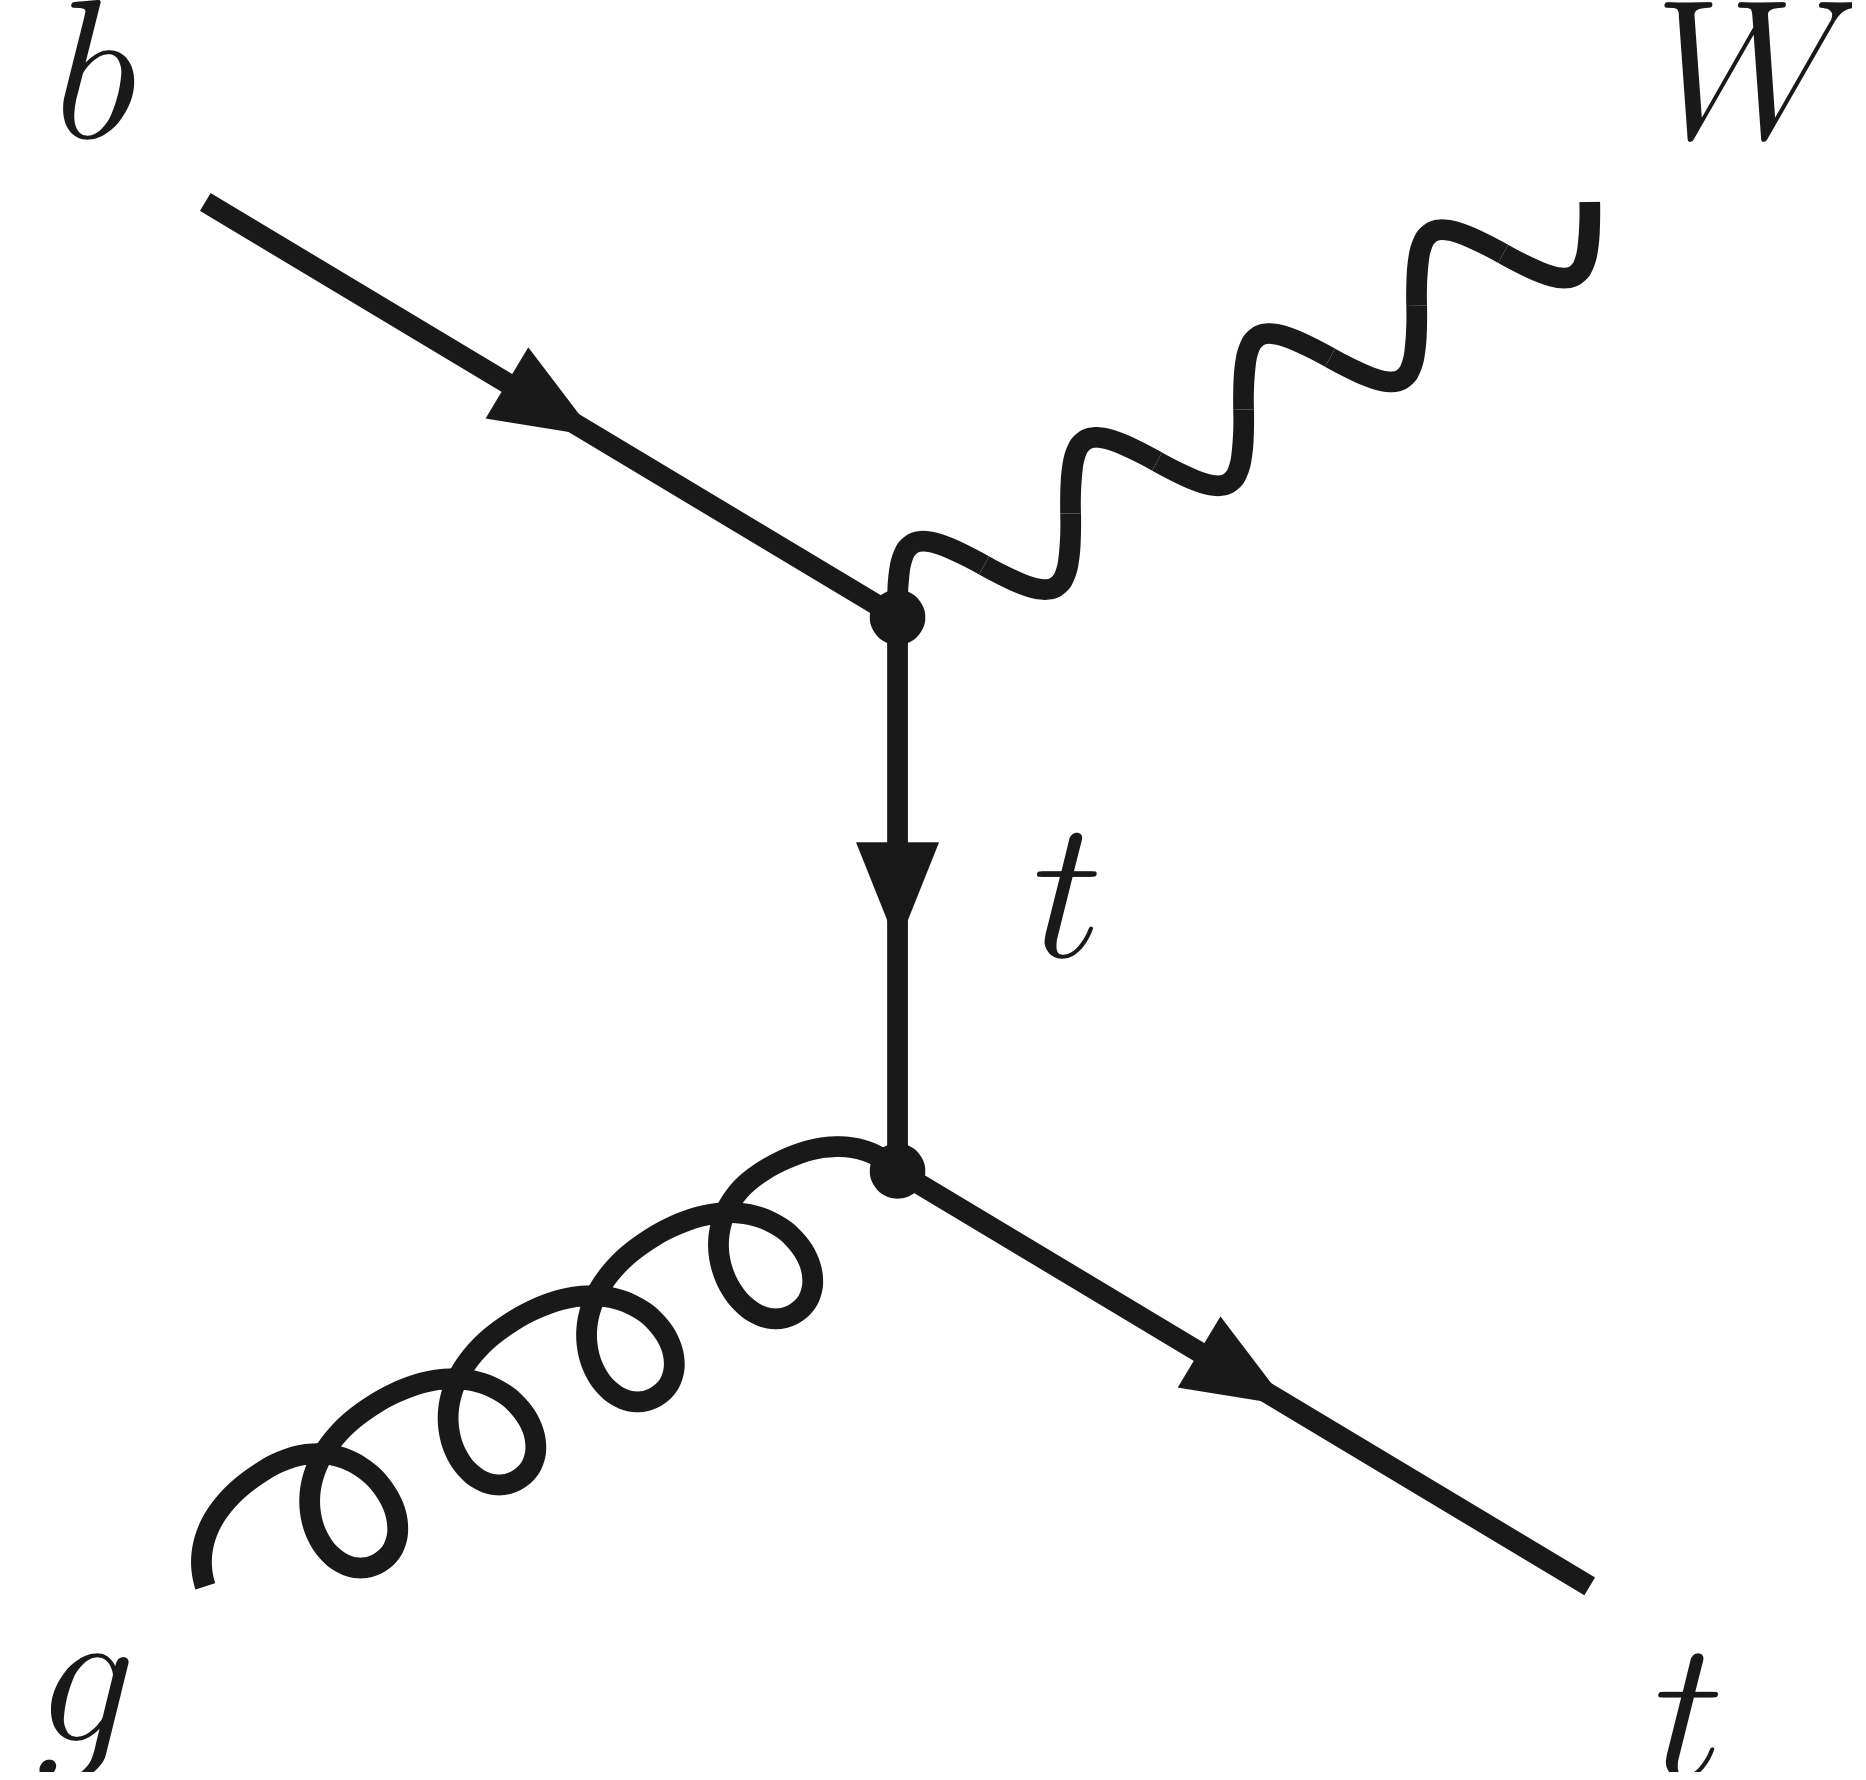
\includegraphics[width=\textwidth]{Chapter1/Single-top-Wt-A}
%         \caption{}
%         \label{fig:Chap1:top:singletop:tW_A}
%     \end{subfigure}
%     \begin{subfigure}[b]{0.3\textwidth}
%         \centering
%         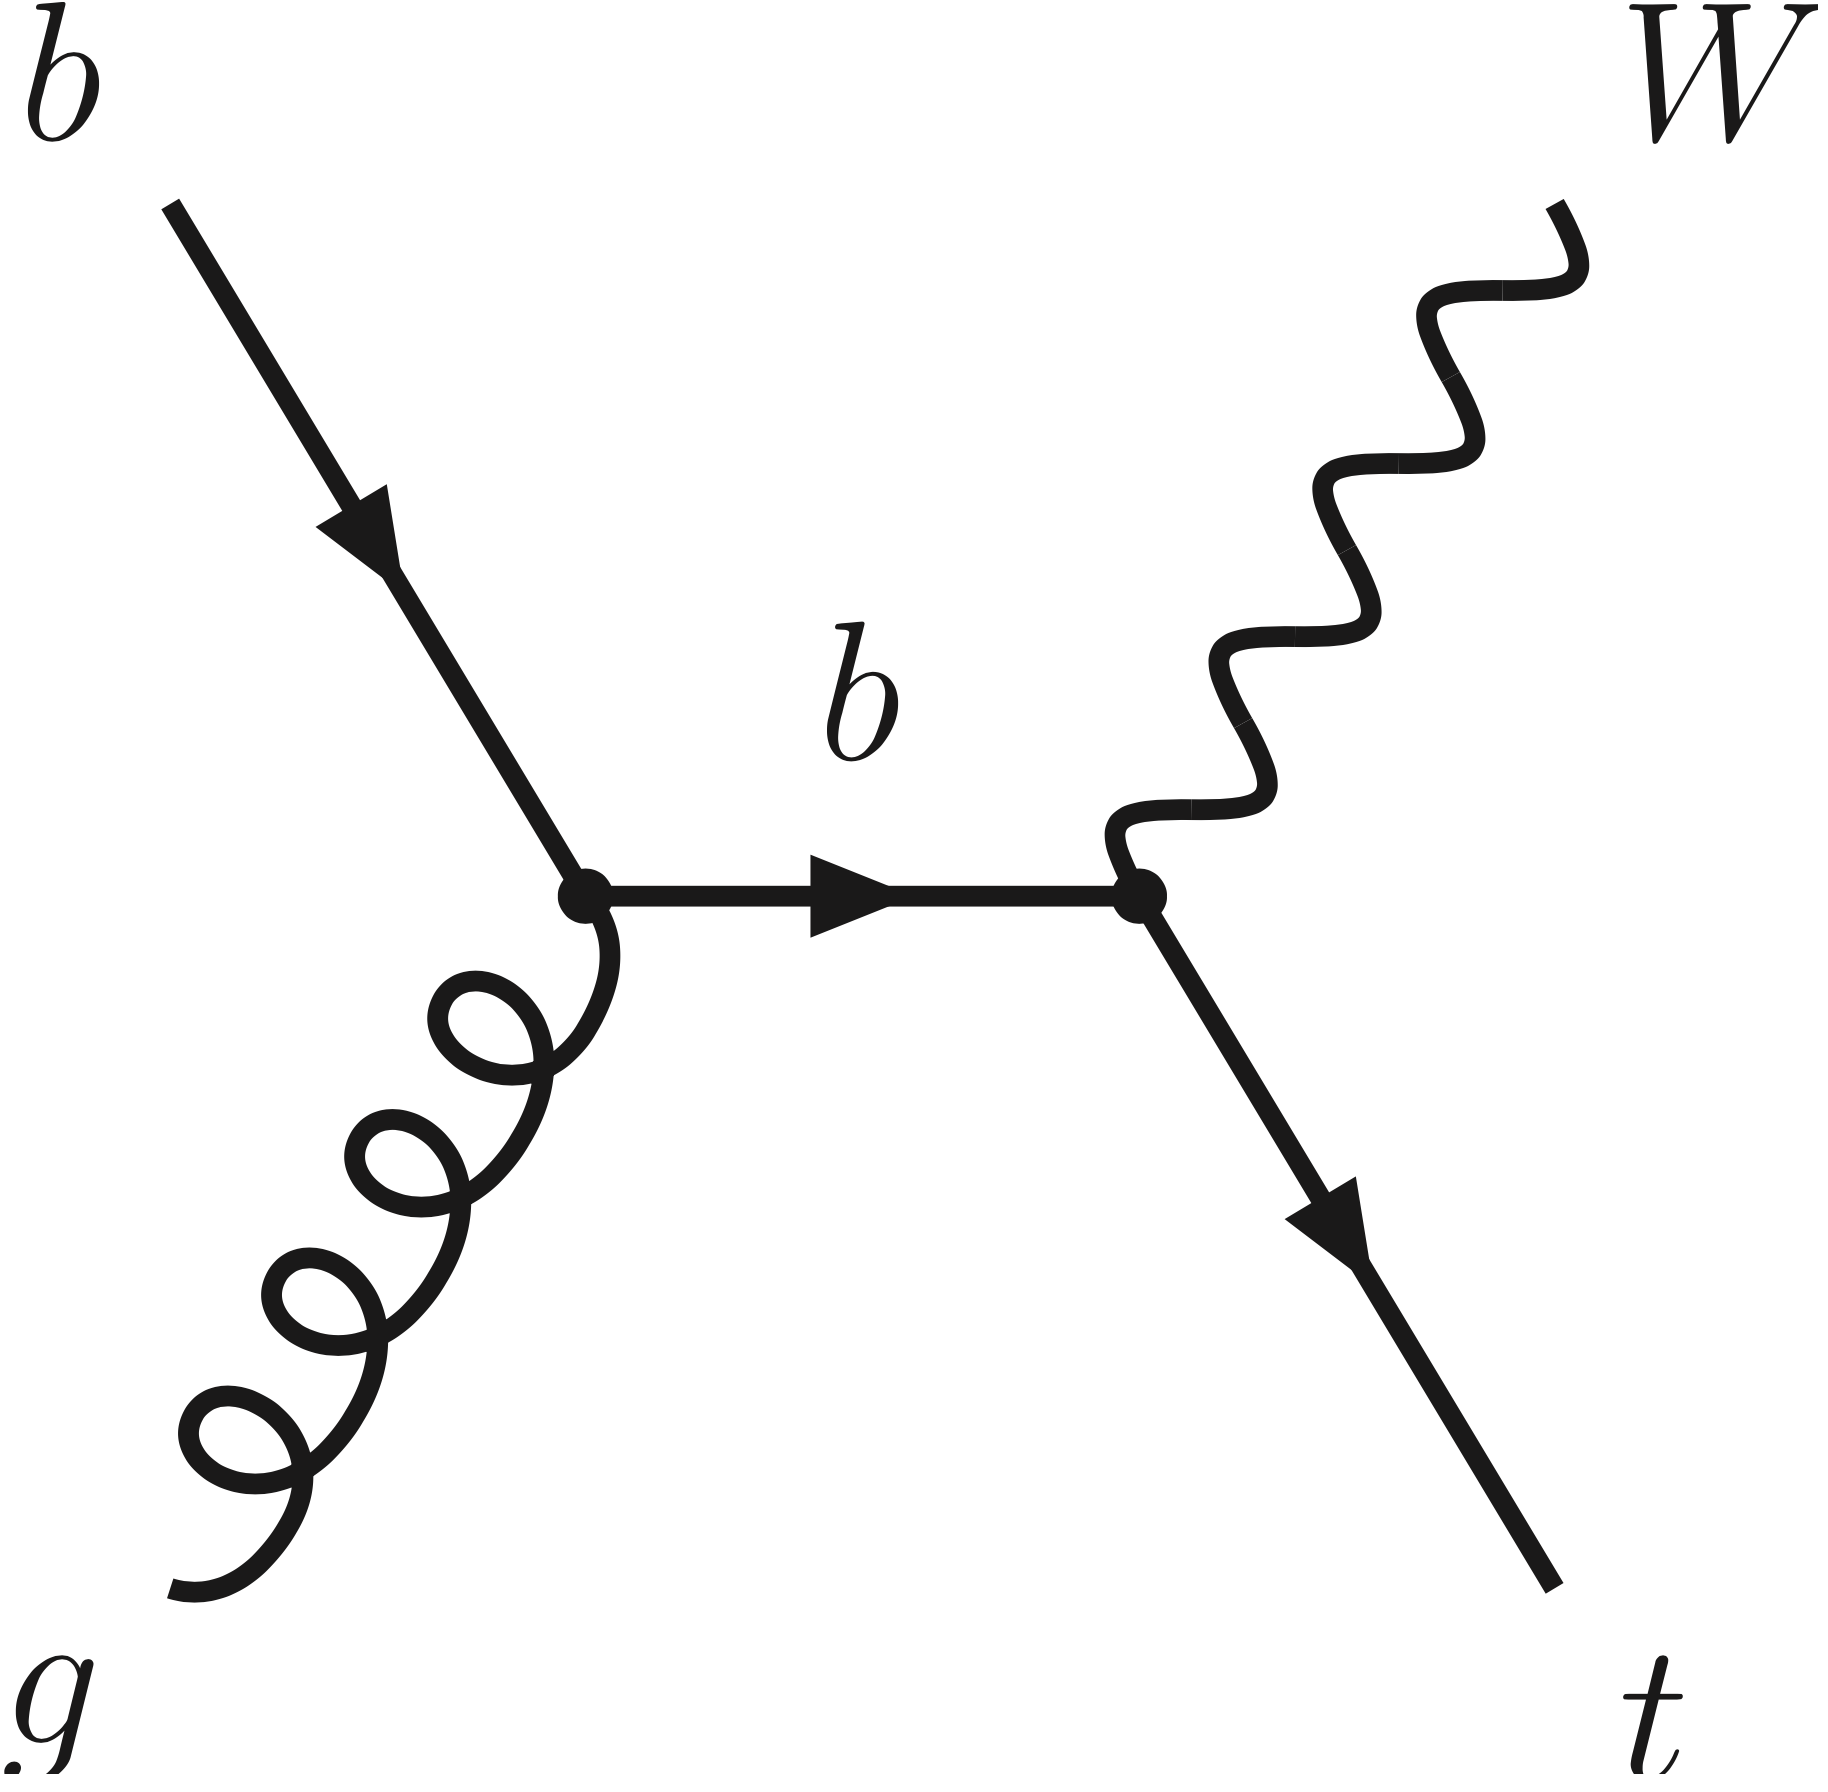
\includegraphics[width=\textwidth]{Chapter1/Single-top-Wt-B}
%         \caption{}
%         \label{fig:Chap1:top:singletop:tW_B}
%     \end{subfigure}
%        \caption{Representative Feynman diagrams for the single-top-quark production in association with a \PW boson.}
%        \label{fig:Chap1:top:singletop:tW}
%\end{figure}
%\end{comment}





%%%%%%%%%%%%%%%%
%                Four tops               %
%%%%%%%%%%%%%%%%
\subsubsection{Four tops}
\label{sec:Chap1:Top:Production:4tops}
%source: 
%		https://inspirehep.net/files/216bcad412f9e5d56fda0820c1b726c9
%		https://atlas.web.cern.ch/Atlas/GROUPS/PHYSICS/CONFNOTES/ATLAS-CONF-2020-013/
The production of four top quarks ($t\bar{t}t\bar{t}$) is a rare SM process that takes place at the LHC 
with a predicted cross-section of $\sigma^{pred}_{t\bar{t}t\bar{t}} = 12.0^{+2.2}_{-2.5}$~fb for \Pproton\Pproton
collisions at $\CM=13$~TeV (calculations at NLO for QCD and EW~\cite{Frederix:2017wme}). 
ATLAS and CMS have measured the $t\bar{t}t\bar{t}$ production cross-section and obtained,
respectively, $\sigma_{t\bar{t}t\bar{t}} = 24^{+16}_{-14}$~fb~\cite{ATLAS:2021kqb} and 
$\sigma_{t\bar{t}t\bar{t}} = 12.6^{+5.8}_{-5.3}$~fb~\cite{CMS:2019rvj}.
While the first measurement does not agree with the theoretical prediction, 
it yields a larger statistical significance. 

% Remove summary plots and Feynman diagrams for the tttt
%\begin{comment}
Figure~\ref{fig:Chap1:top:4top_xsec} presents the $\sigma_{t\bar{t}t\bar{t}}$ measurements 
by ATLAS and CMS compared to the quoted theoretical calculation. 

The representative Feynman diagrams are presented in Figure~\ref{fig:Chap1:top:4Top:Feyn}, 
where of particular interest is the production by the exchange of a Higgs boson. 
This indicates a strong dependence of this type of production
with the top-quark-Yukawa coupling.

\begin{minipage}[t]{0.55\textwidth}
\begin{flushleft}
\noindent
\vskip0pt
	%\begin{figure}
    	%\centering
    	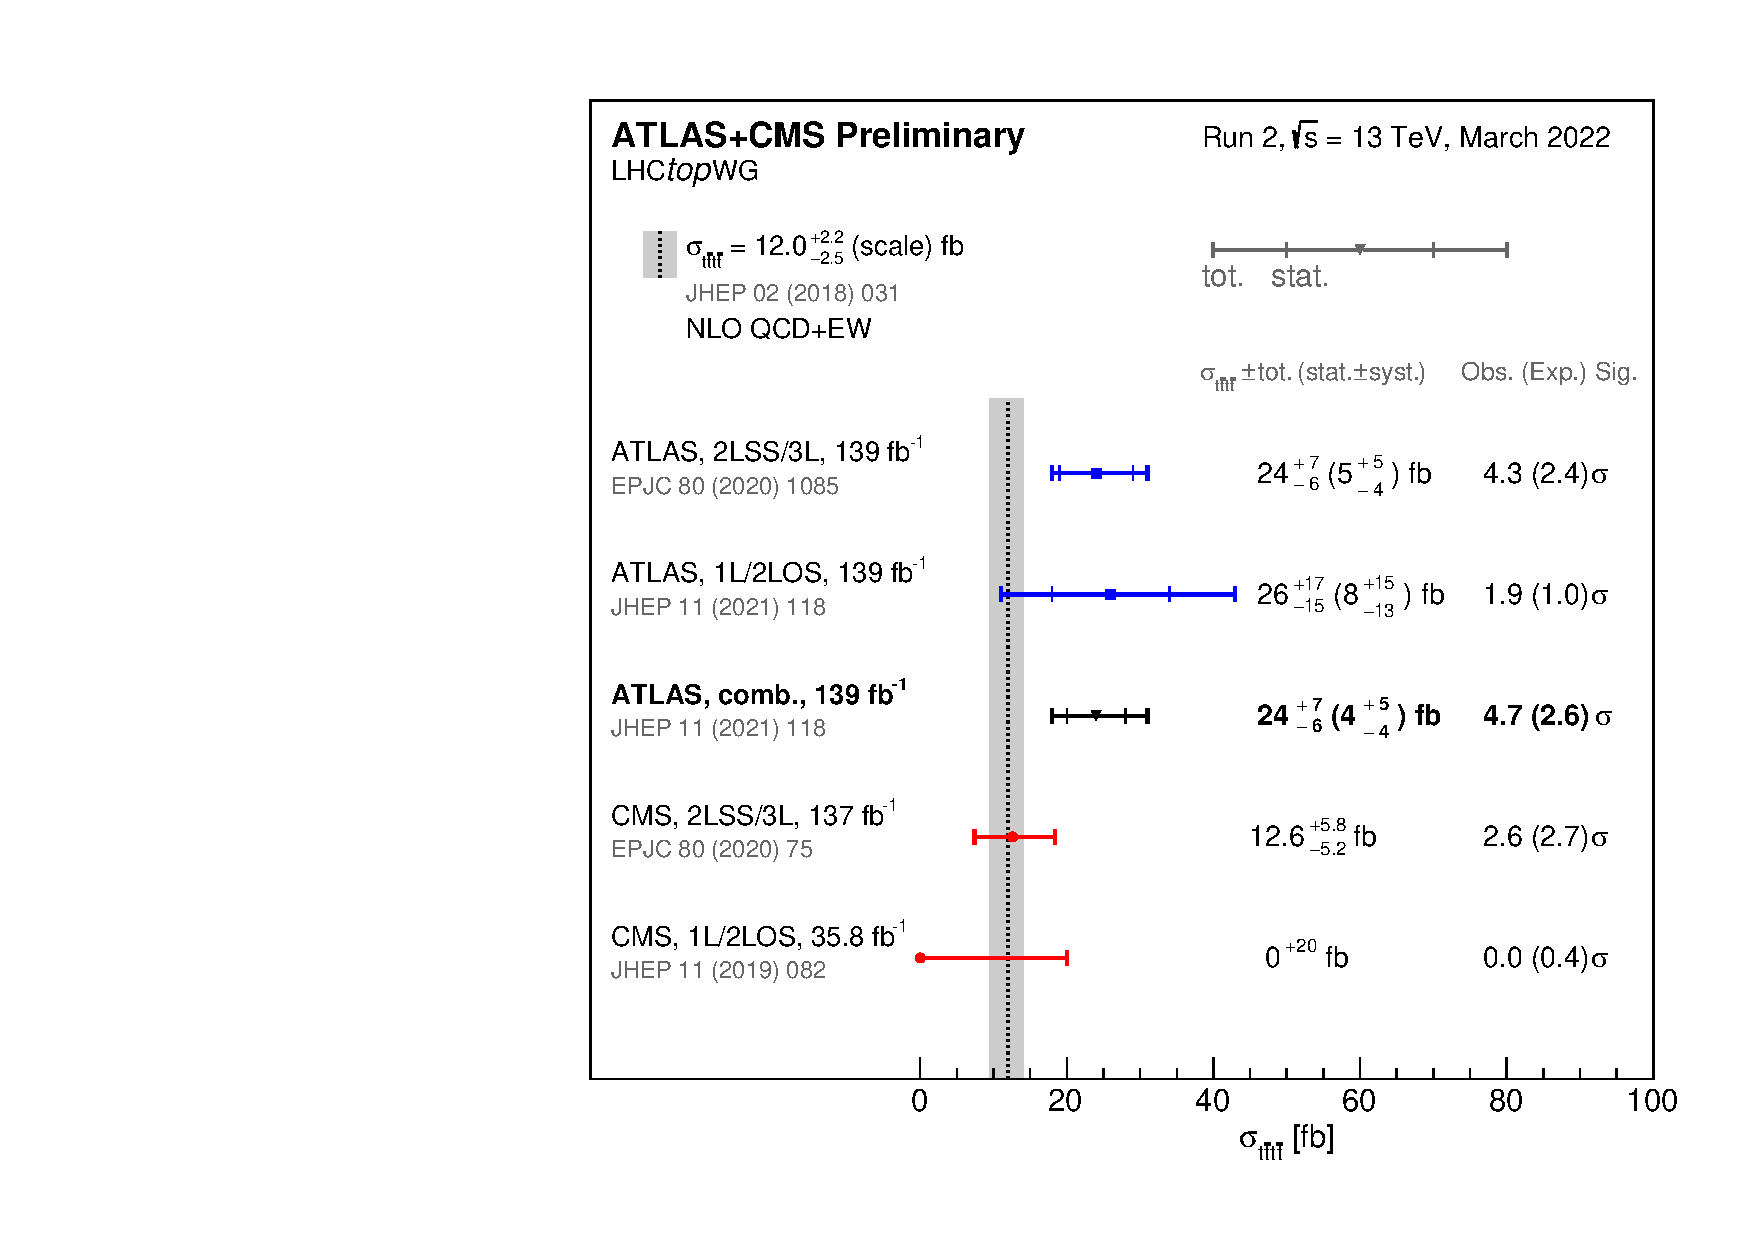
\includegraphics[width =\textwidth]{Chapter1/fourtop_summary_mar22}
    	\captionof{figure}{Summary of the ATLAS and CMS measurements of 
	the $t\bar{t}t\bar{t}$ production cross-sections at $13$~TeV in various channels.
	\pablo{Quitar figura, mencionar el resultado más preciso combinado de ATLAS y su significancia.}}
        \label{fig:Chap1:top:4top_xsec}
        \strut
	%\end{figure}
\end{flushleft}	
\end{minipage}\hfill
\begin{minipage}[t]{0.4\textwidth} 
%\setbox0=\hbox{T} % tallest letter of the first line of other minipage
\vskip0pt
	%\begin{multicols}{2}
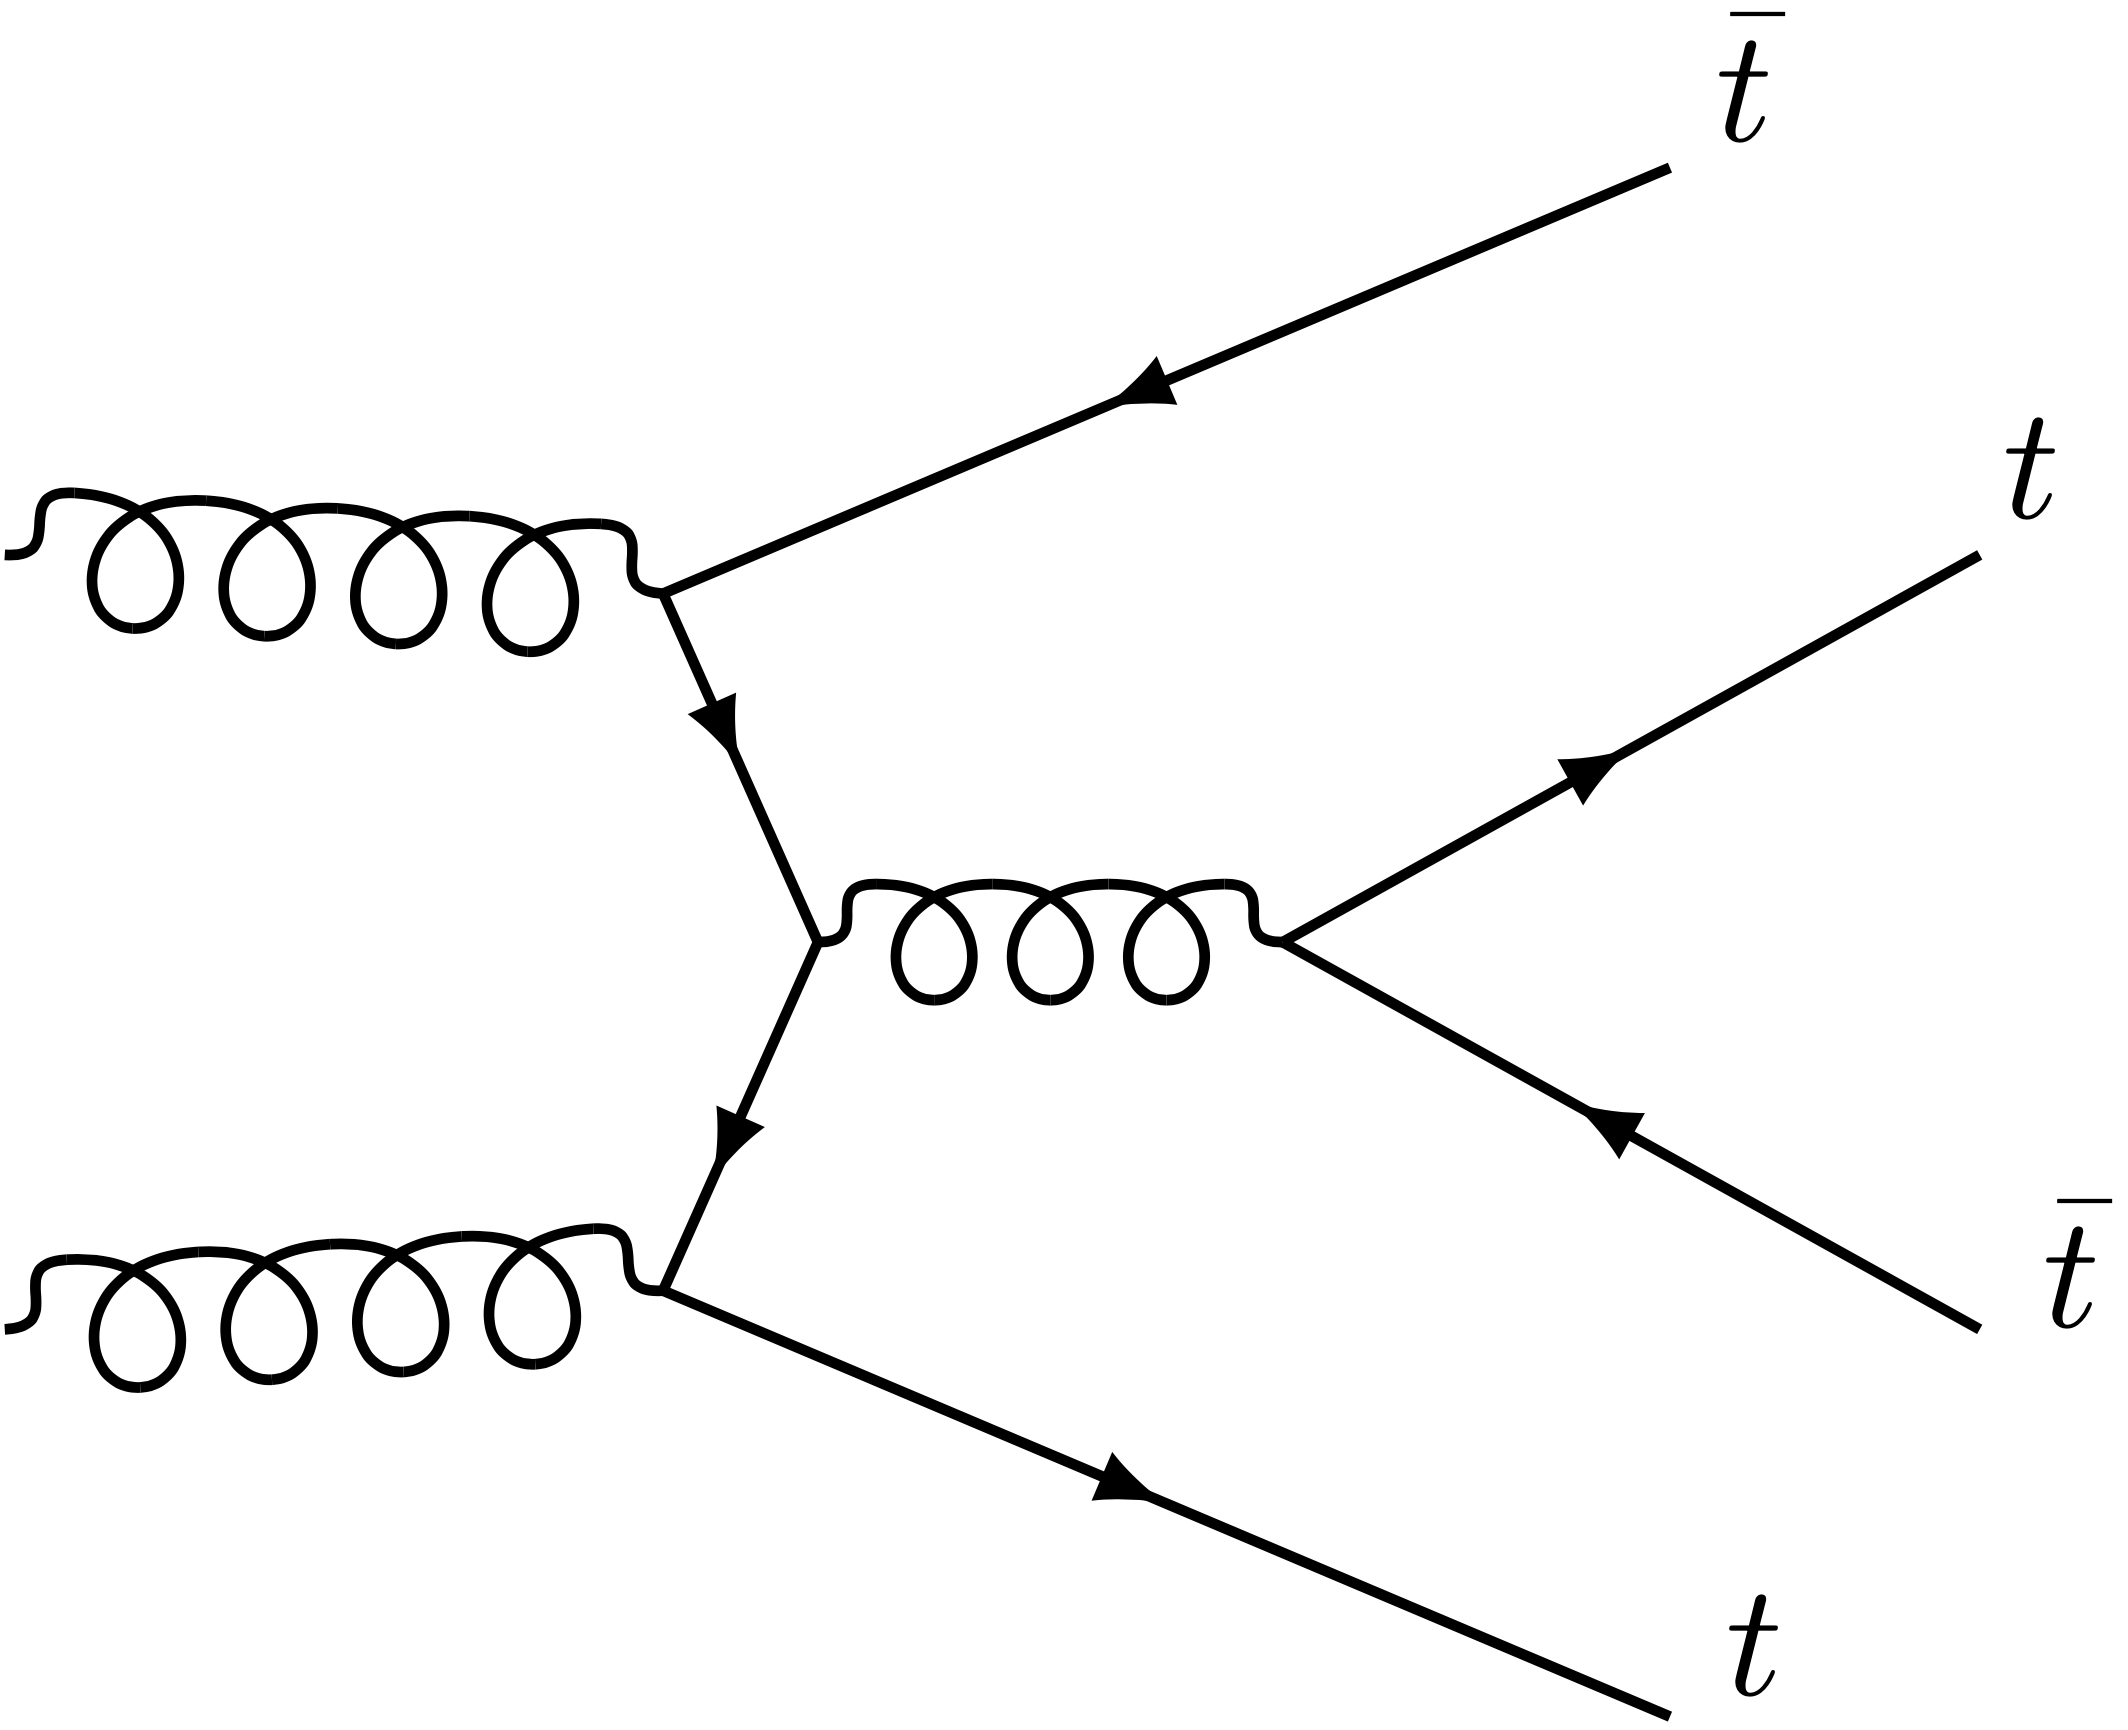
\includegraphics[width=0.85\linewidth]{Chapter1/Feynman_FourTop_A}\par 
    	%\end{multicols}
	%\begin{multicols}{2}
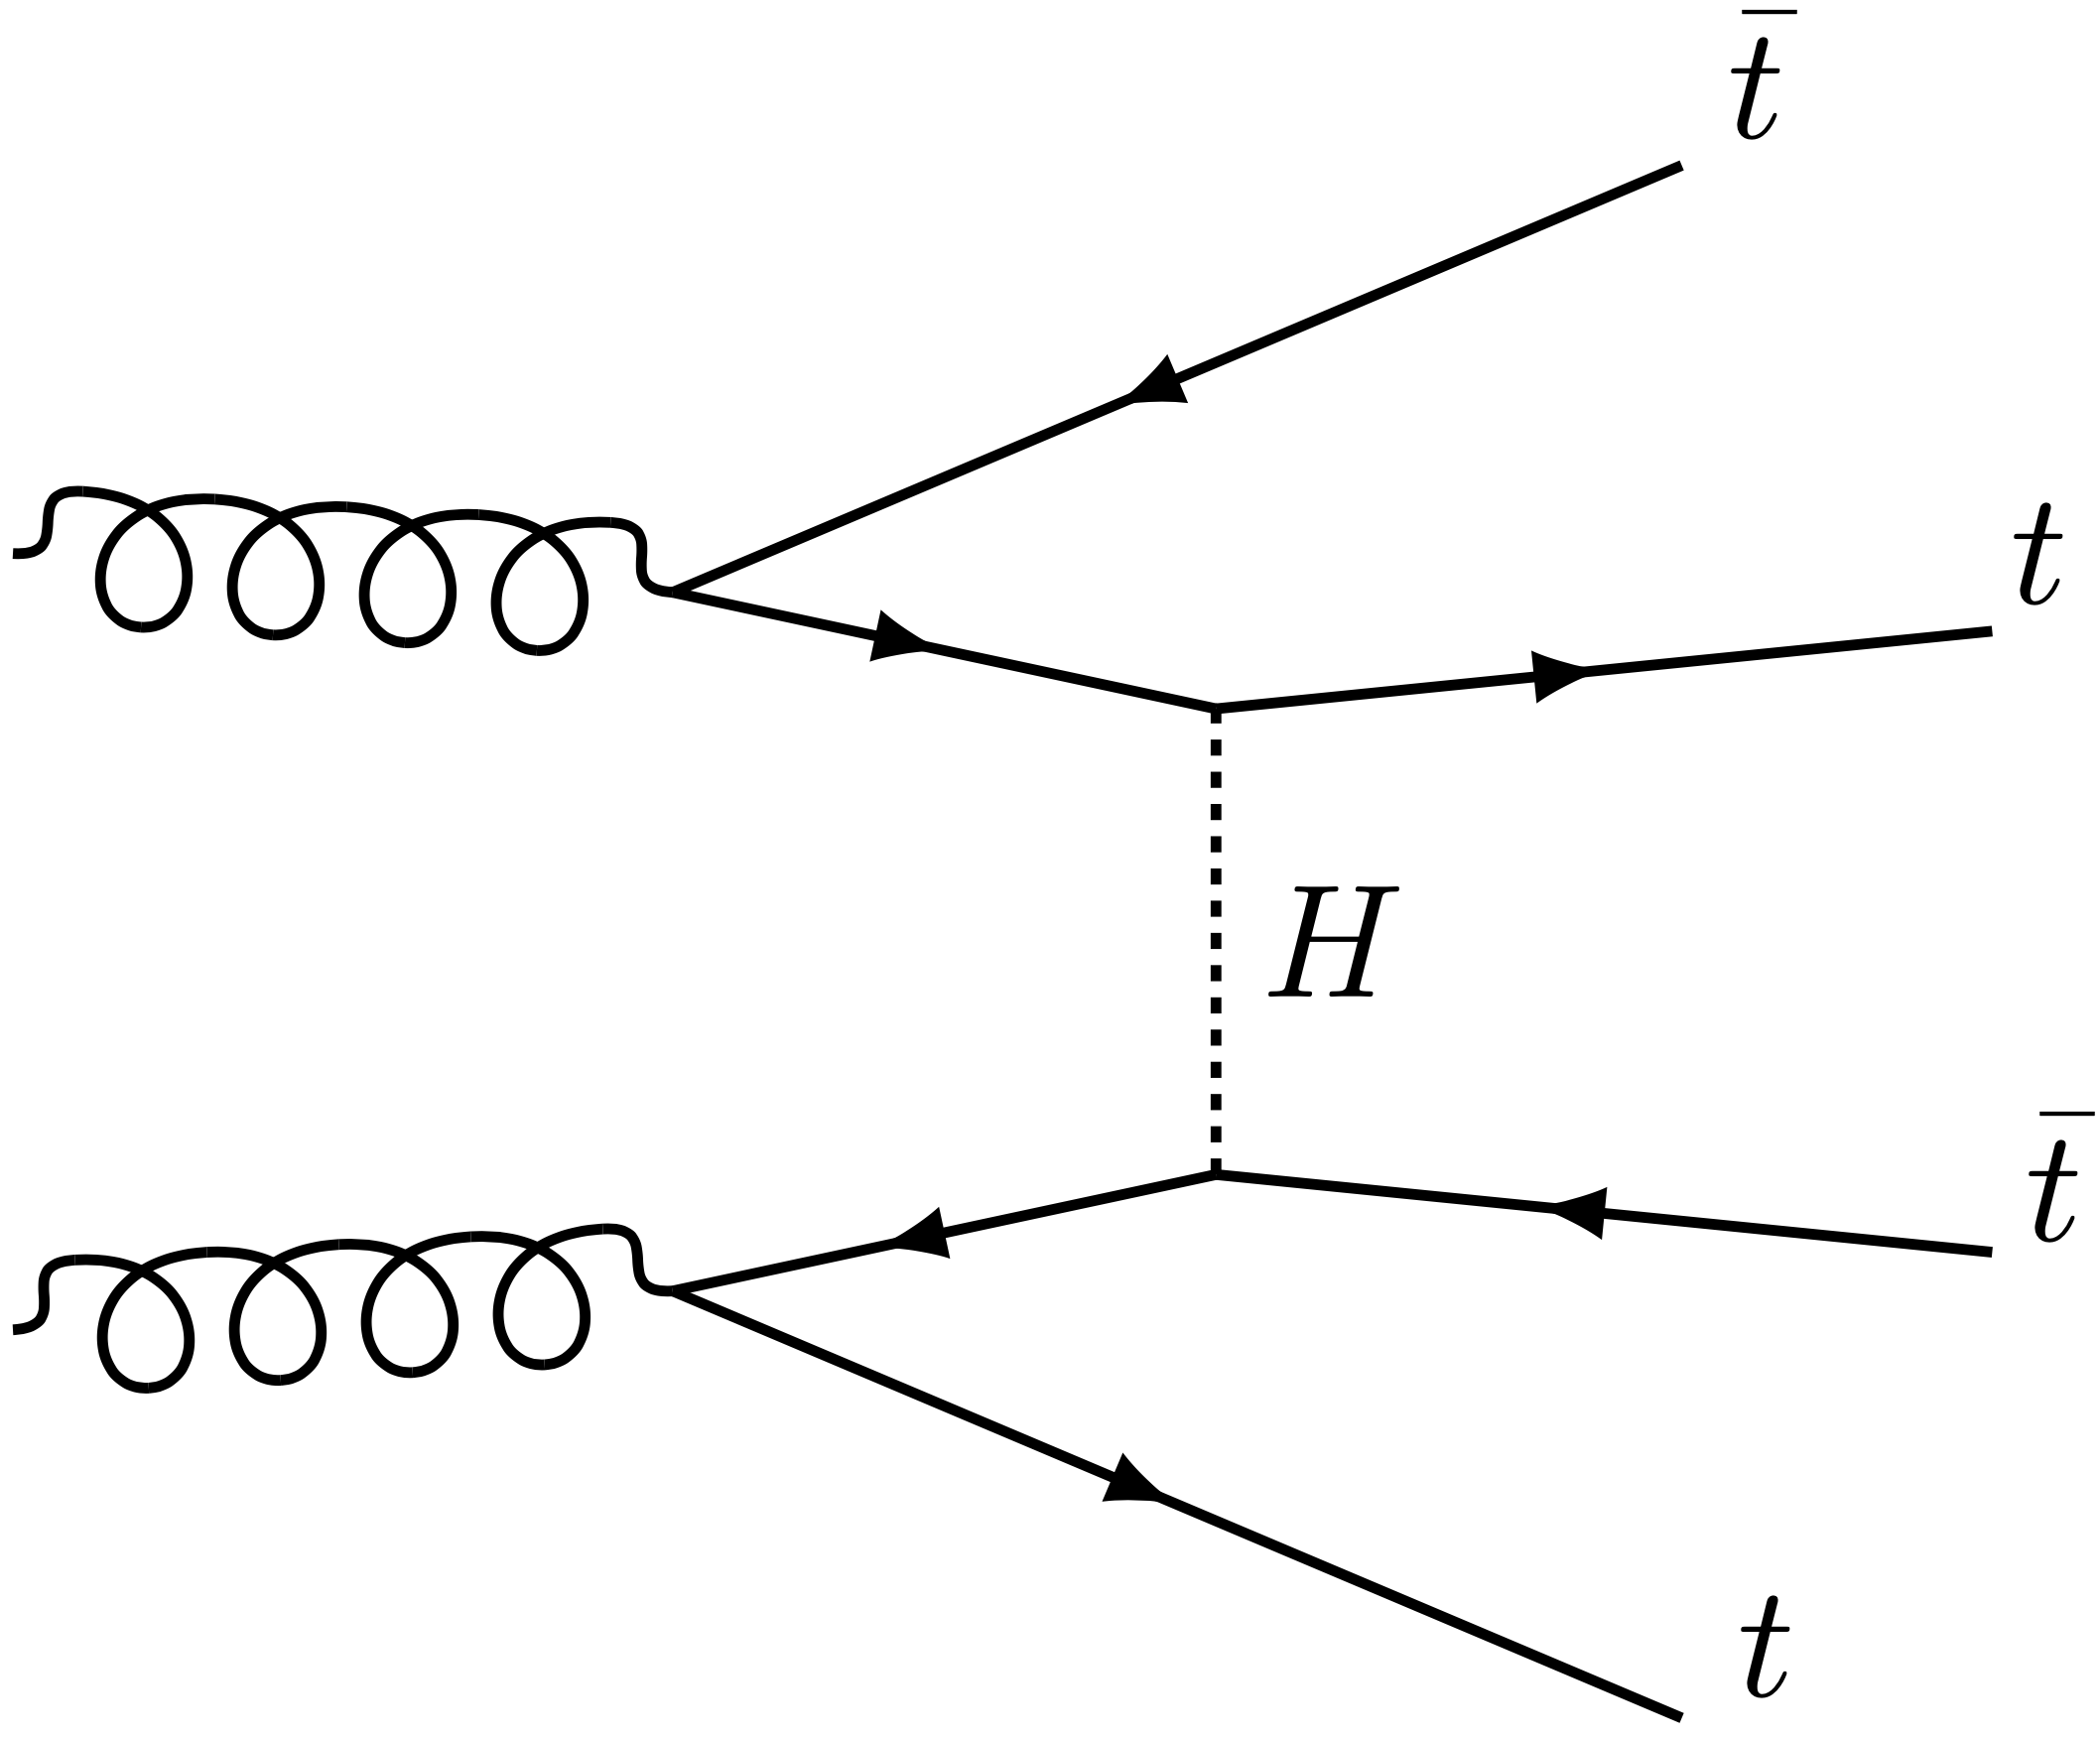
\includegraphics[width=0.85\linewidth]{Chapter1/Feynman_FourTop_B}\par
	%\end{multicols}
	\captionof{figure}{Representative Feynman diagrams for the $\Pgluon\Pgluon \rightarrow t\bar{t}t\bar{t}$ production.}
        \label{fig:Chap1:top:4Top:Feyn}
\end{minipage}
% Avoid the vertical space in the minipage envirorment:
% https://tex.stackexchange.com/questions/331617/too-much-vertical-space-before-a-minipage-environment
%\end{comment}

\end{comment}

%%%%%%%%%%%%%
%                tt-X              %
%%%%%%%%%%%%%
\subsubsection{Associated \ttX production}
\label{sec:Chap1:Top:Production:ttbar_plus_X}
% Measurements for top+X: https://atlas.web.cern.ch/Atlas/GROUPS/PHYSICS/PUBNOTES/ATL-PHYS-PUB-2022-049/
The associated-top-quark productions are important processes to measure
the coupling of the top quark to other particles of the SM. 
When a pair of top quarks is produced along with another particle 
the process is referred to as $\ttX$. The most relevant $\ttX$ productions
are those in which the pair is produced together with \PW, \PZ or \Pgamma bosons.
From these, \ttW and \ttZ play a role in the analysis carried in this thesis.
These two processes along with \ttbar are the three most relevant backgrounds
in one of the channels of the analysis performed in this thesis.
%in the \tHq production with two light leptons and one hadronic tau when
%the light leptons have the same electric charge (\dilepSStau). This is, precisely,
%one of the two channels studied in this thesis.

%The \ttH process is not included in the \ttX section but described in Section~\ref{sec:Chap1:top-Higgs}. 
%The different production diagrams for \ttW are shown
%in Figure~\ref{fig:Chap1:top:ttX:ttW_Feynman}. 
\begin{comment}
\begin{figure}
        \begin{subfigure}[b]{0.25\textwidth}
                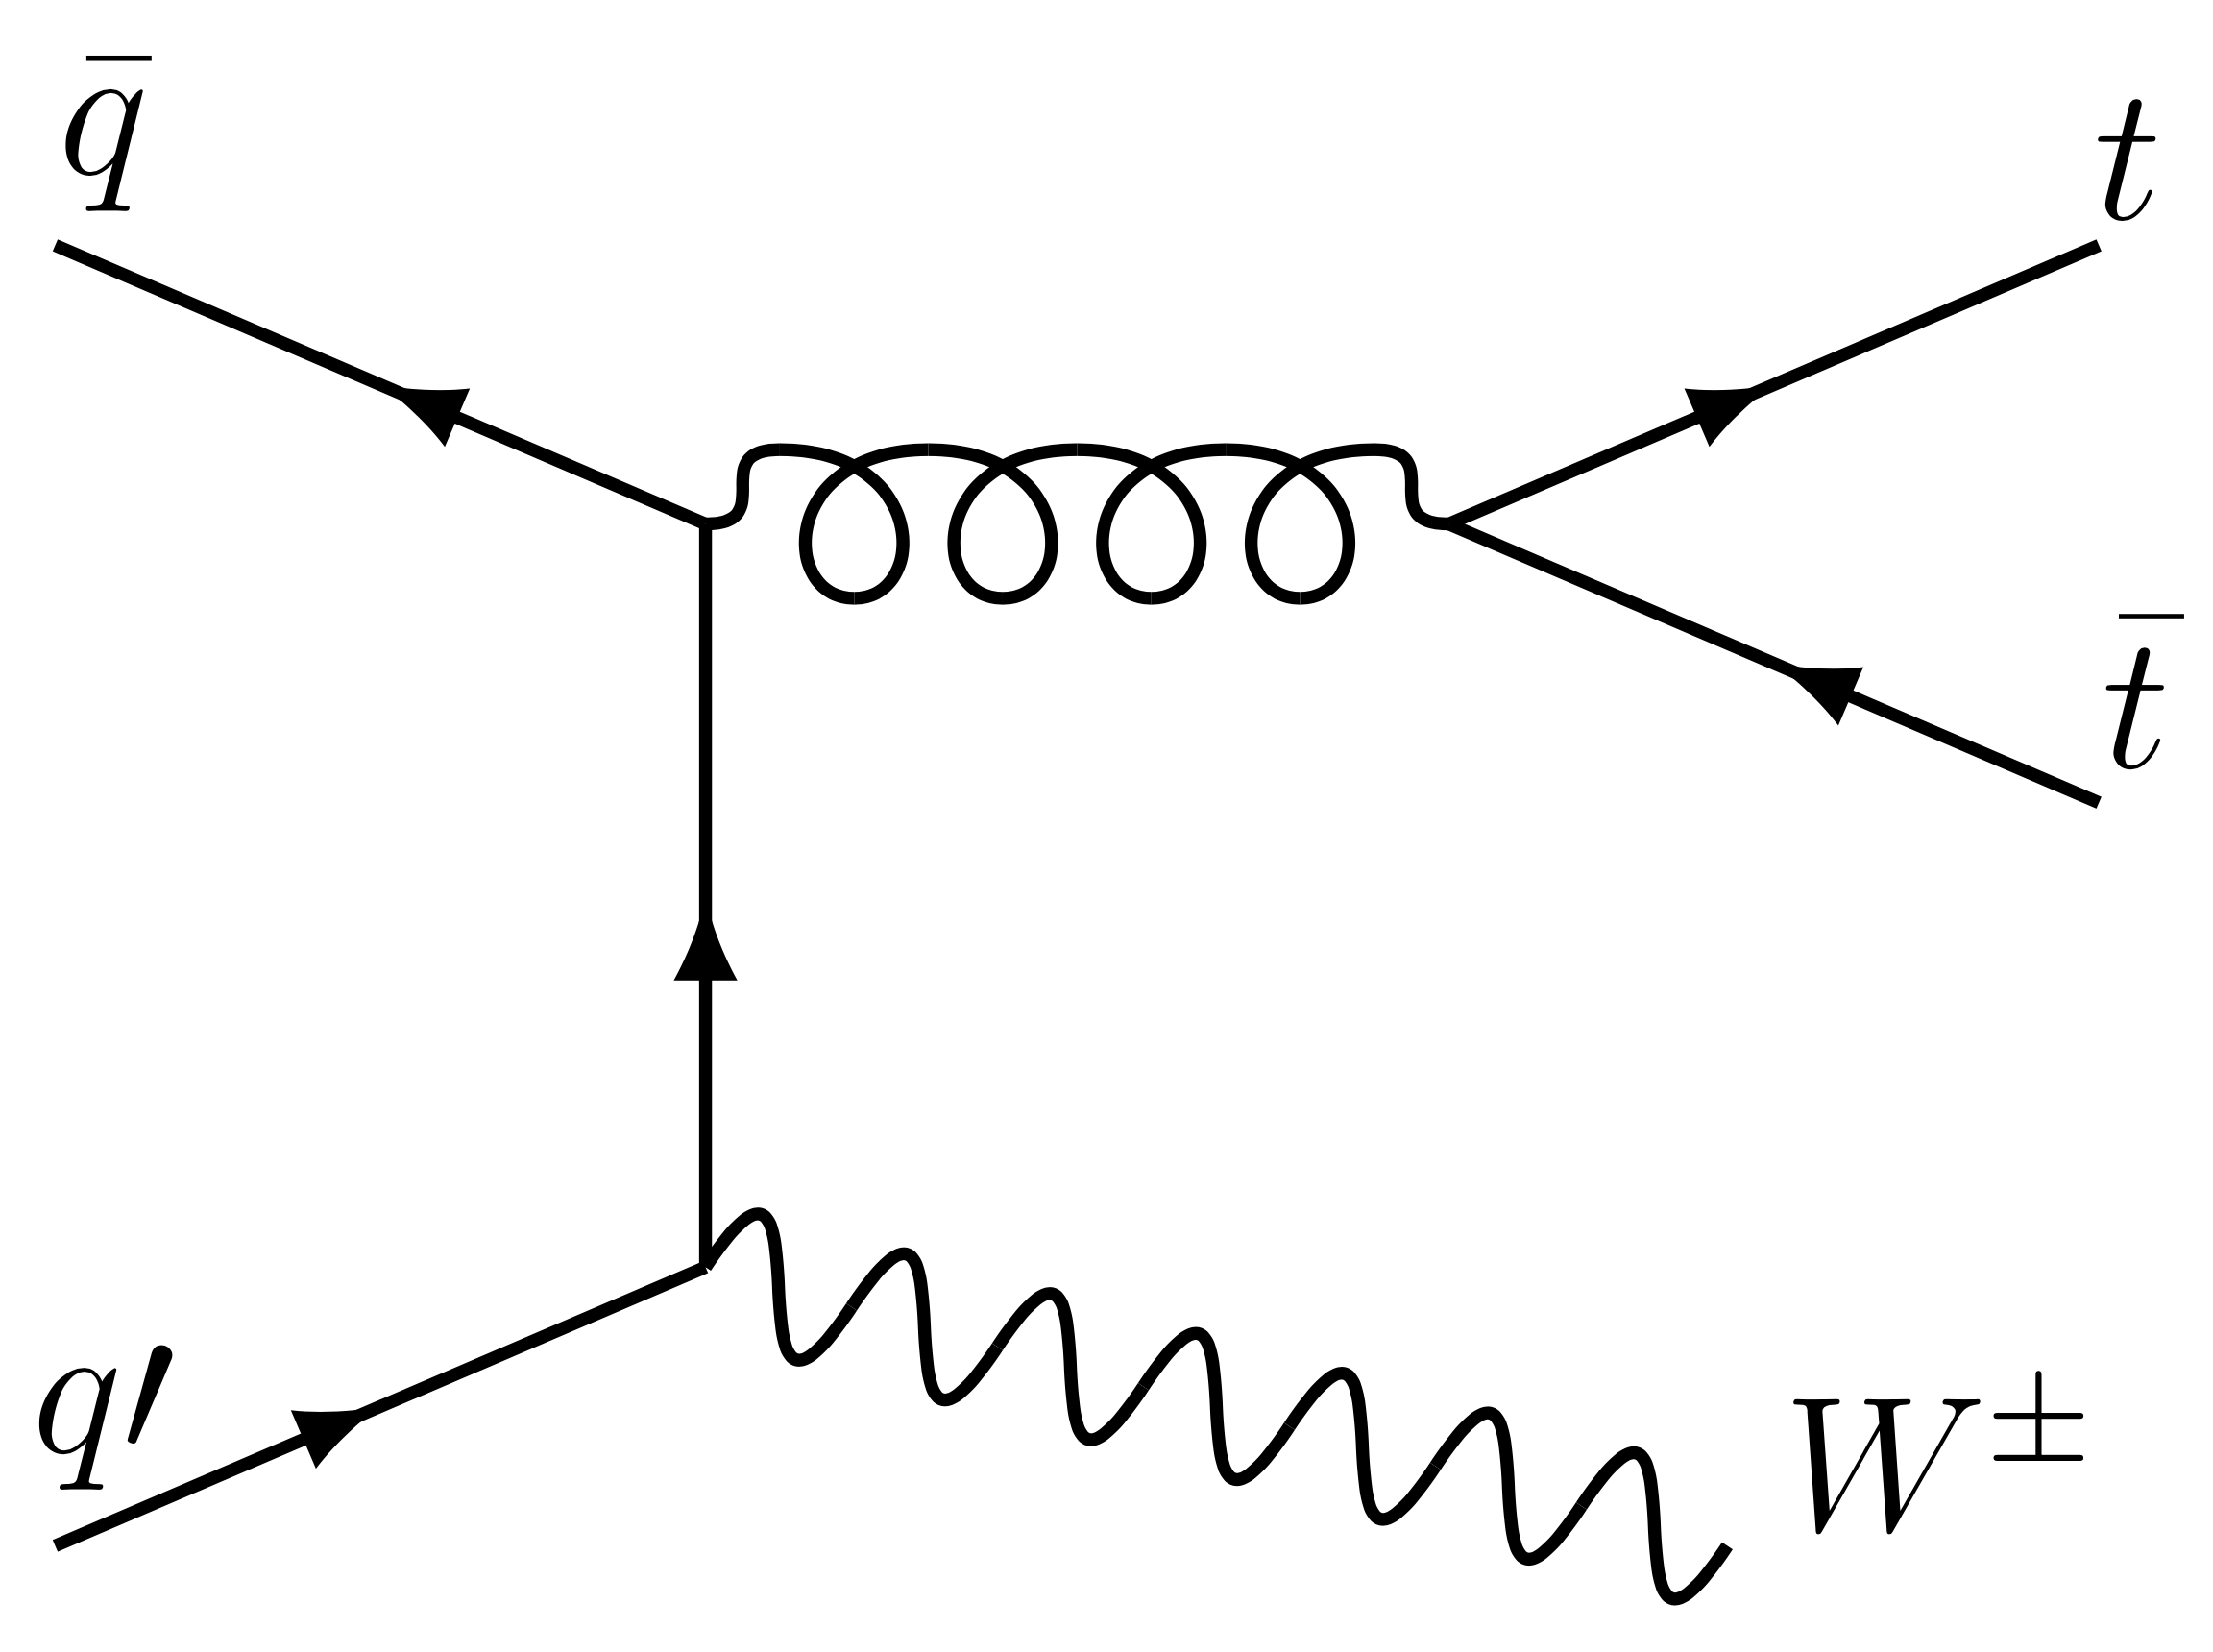
\includegraphics[width=\linewidth]{Chapter1/ttW_qq_A}
                \caption{}
                %\label{}
        \end{subfigure}%
        \begin{subfigure}[b]{0.25\textwidth}
                \includegraphics[width=\linewidth]{Chapter1/ttW_qq_B}
                \caption{}
                %\label{}
        \end{subfigure}%
        \begin{subfigure}[b]{0.25\textwidth}
                \includegraphics[width=\linewidth]{Chapter1/ttW_gq_A}
                \caption{}
                %\label{}
        \end{subfigure}%
        \begin{subfigure}[b]{0.25\textwidth}
                \includegraphics[width=\linewidth]{Chapter1/ttW_gq_B}
                \caption{}
                %\label{}
        \end{subfigure}
        \caption{Representative Feynman diagrams for \ttW production.
        Left diagrams show the $\bar{q}q'\rightarrow \ttW$ processes 
        and right ones the $\bar{q}g\rightarrow \ttW q'$ production. \pablo{igual tampoco
        	hace falta enseñar estos diagramas}}\label{fig:Chap1:top:ttX:ttW_Feynman}
\end{figure}
\end{comment}

The cross-sections for the \ttW, $\ttbar \gamma$ and $\ttbar \PZ$ productions 
are measured by the ATLAS and CMS collaborations. % with a large degree of agreement between the 
%two experiments. %The ATLAS measurements and NLO calculations for \ttW are 
%$\sigma_{\ttW} = 0.87 \pm 0.27\,\text{pb}$~\cite{ATLAS:2019fwo}, 
%$\sigma^{pred}_{\ttW} = 0.72^{+0.08}_{-0.09}\,\text{pb}$~\cite{ATLAS:2018fwq}. For the $\ttbar \gamma$
%process $\sigma_{\ttbar \gamma} = 0.798 \pm 0.055\,\text{pb}$~\cite{ATLAS:2020yrp}, 
%$\sigma^{pred}_{\ttbar \gamma} = 0.77\pm0.14\,\text{pb}$. The $\ttbar \PZ$ production yields
%a cross-section of $\sigma_{\ttbar \PZ} = 0.99 \pm 0.13\,\text{pb}$~\cite{ATLAS:2021fzm}, 
%$\sigma^{pred}_{\ttbar \PZ} = 0.86^{+0.09}_{-0.11}\,\text{pb}$~\cite{Kulesza:2020nfh}. 
These are presented in 
Figure~\ref{fig:Chap1:top:ttX:Cross-Sec}. For the three \ttX, the cross-sections
are small in comparison to \ttbar and single top-quark productions.
However, with the complete LHC Run 2 data event sample it is possible to explore these productions, which
are also sensitive to new physics~\cite{ATLAS:2020hpj}. 
The associated production of a \ttbar pair with a Higgs boson (\ttH) is another important
type of \ttX production and it is described in Section~\ref{sec:Chap1:ttH}.

\begin{figure}[h]
    \centering
    \includegraphics[width = 0.9\textwidth]{Chapter1/xsec_2023_ttX}
    \caption{Summary of the ATLAS and CMS measurements of the $\ttbar X$ production 
    cross-sections at $\CM =13$~TeV. Here $X$ means either $\PW$, $\PZ$ or $\Pgamma$.} %\pablo{Esta figura se queda porque ahorra tenxto.}} %Update from https://twiki.cern.ch/twiki/bin/view/LHCPhysics/LHCTopWGSummaryPlots#Pair_production_cross_section
    \label{fig:Chap1:top:ttX:Cross-Sec}
\end{figure}

%%%%%%%%%%%%%
%                tX              %
%%%%%%%%%%%%%
\subsubsection{Associated \tX production}
\label{sec:Chap1:Top:Production:top_plus_X}
Not only the top-quark pairs but also the single top quark can be produced
in association with other particles (\tX).
This thesis focusses precisely on the search of a \tX production, the
one in which the single top quark is produced along a Higgs boson and
an additional parton (\tHq). The features of the single-top-quark production 
in association with a Higgs boson are discussed in more detail in 
Section~\ref{sec:Chap1:tHq}.

Apart from being the signal process, the \tX production also plays a role
in the background since the \tZq process
is one of the backgrounds more difficult to separate from the \tHq signal. 
%in the final state characterised by two light-flavour leptons and one hadronic tau in the scenario in which
%the light leptons have a different electric charge (\dilepOStau).

%This type of production
%play an important role in the \tHq searches carried in this thesis since the \tZq process
% is one of the backgrounds more difficult to separate 
The other associated $\tX$ production of the EW type is the $\Ptop q \Pgamma$, in which the
top quark is produced along with a photon. Both \tZq and $\Ptop q \Pgamma$
are sensitive to beyond the SM (BSM) physics like flavour-changing neutral currents or vector-like quarks.
ATLAS and CMS have measured both processes and have found an agreement with the SM model, as 
as can be seen in  Figure~\ref{fig:Chap1:top:tX:Cross-Sec}.
%while for \tZq a good SM agreement
%is found, this is not the case for the $\Ptop q \Pgamma$ as can be seen in 
%Figure~\ref{fig:Chap1:top:tX:Cross-Sec}.

%In this work, the most relevant $\tX$ mode is the 
%single-top-quark production in association with a Higgs boson
%This is the main process to search for in the thesis and its features
%are discussed in more detail in Section~\ref{sec:Chap1:tHq}.

\begin{figure}
    \centering
    \includegraphics[width = 0.9\textwidth]{Chapter1/xsec_2023_tX.pdf}
    \caption{Summary of the ATLAS and CMS measurements of the $\tX$ production 
    cross-sections at $\CM =13$~TeV. Here, $X=\PZ$, $\Pgamma$ and \PW. The \tHq process 
    in not included in this summary plot but the work developed in this thesis aims to help
    to provide better limits on its cross-section.} %Update from https://twiki.cern.ch/twiki/bin/view/LHCPhysics/LHCTopWGSummaryPlots#Pair_production_cross_section
    \label{fig:Chap1:top:tX:Cross-Sec}
\end{figure}







%%%%%%%%%%%%%%%%%
%                Top decay               %
%%%%%%%%%%%%%%%%%
\subsection{Top-quark decay}
As anticipated in Section~\ref{sec:Chap1:Top:Production:SingleTop}, due to the large 
value of the $V_{tb}$ element of the CKM matrix, the 
top quark is expected to decay almost entirely ($\sim 99.8 \%$) %through the medium of the \Wtb vertex 
to a \Pbottom quark and a \PW boson ($\Ptop \rightarrow \PW \Pbottom$).
%The \tWb vertex and the decay chain of the top quark is 
%represented in Figure~\ref{fig:Chap1:top:decay:TopQuarkDecay}.
The final-state decay is classified according to the subsequent decay of the \PW boson.
Since the \PW bosons are massive vector bosons,
their lifetime is very short ($\tau_{\PW} \approx 3\times10^{-25}$~s) and hence they will
rapidly decay to leptons or quarks that will form hadrons. 
Due to its large mass, the \PW boson can decay to any quark except the top quark. 
For the \PWplus, the branching ratios\footnote{For each decay mode, the branching ratio (BR) is defined as the fraction times that the particle decays in that particular mode with respect to total possible decays.} (BRs) for the different decay modes are~\cite{Workman:2022ynf}:
\begin{align*}
	\PWplus &\rightarrow \Ppositron \Pneutrino_{e} 			&& (10.71 \pm 0.16)\%, \\
	\PWplus &\rightarrow \APmuon \Pneutrino_{\mu} 			&& (10.63 \pm 0.15)\%, \\
	\PWplus &\rightarrow \APtauon \Pneutrino_{\tau} 			&& (11.38 \pm 0.21)\%, \\
	\PWplus &\rightarrow \Pquark \APquark \textrm{ (hadrons)}	&& (67.41 \pm 0.27)\%, \\
	\PWplus &\rightarrow \textrm{invisible}					&& (1.4 \pm 2.9)\% .
\end{align*} 
For the conjugate proceses involving the \PWminus, the BRs are the same. Therefore, the \PW boson decay 
and consequently the top-quark decay can be classified either as leptonic or hadronic. 


%\begin{figure}
%    \centering
%    \includegraphics[width = 0.3\textwidth]{Chapter1/TopQuarkDecay}
%    \caption{Decay of a top quark to a \Pbottom quark and a \PW boson. The \PW boson can 
%    		decay either leptonically to a neutrino and a lepton
%    		or hadronically to a pair of light-flavour quarks. In the hadronic \PW decay, 
%		a jet triplet is formed along with the \Pbottom quark.}
%    \label{fig:Chap1:top:decay:TopQuarkDecay}
%\end{figure}







%%%%%%%%%%%%%%%%%%%%
%                Top polarisation               %. Not including polarisation in the thesis
%%%%%%%%%%%%%%%%%%%%
\subsection{Top-quark properties}
As commented, the top quark exhibits unique properties and plays a pivotal role in many analyses conducted at the LHC. 
Some of the key investigations related to the top quark are:

\begin{itemize}
	\item \textbf{Charge asymmetry in \ttbar production}: This refers to the subtle deviation observed between the rapidity distributions of top quarks and top antiquarks when produced in pairs~\cite{ATLAS:2022wec}.
	
	\item \textbf{Polarisation of \PW bosons in top-quark decays}: A measurement of the polarisation of the \PW bosons is conducted by quantifying the fractions of longitudinally, left-handed, and right-handed polarised \PW bosons~\cite{ATLAS:2022rms}.
	
	\item \textbf{Top--antitop-quark energy asymmetry}: Analogous to the charge asymmetry, this research focuses on scenarios where the top-quark pair is produced in association with a high-\pT jet~\cite{ATLAS:2021dqb}.
	
	\item \textbf{Top-quark-pair spin correlations}: Due to the  short lifetime of the top quark, its spin information can be extracted from its decay products. Nonetheless, not all decay particles carry the spin information equivalently.  Charged leptons emanating from leptonically decaying \PW bosons almost wholly encapsulate the spin information of the top quark~\cite{ATLAS:2019zrq}.
	
	\item \textbf{Flavour changing neutral currents (FCNCs):} A FCNC is a process where a quark 
	of one flavour changes into a quark of another flavour, without a change in its electric charge. 
	Top quarks, due to their large mass, are particularly interesting when it comes to FCNCs. 
	The top quark can decay through FCNC processes to lighter quarks in association with a photon, \PZ boson, or gluon.
	%Given that the Higgs boson possesses a smaller mass than the top quark, any emergence of 
	%FCNC would predominantly manifest during top-quark decay~\cite{ATLAS:2018jqi}.
	% FCNC are forbidden at tree level by the SM. This is due to the GIM mechanism.
	% However, FCNC can occur at higher orders
	
	\item \textbf{Top-quark polarisation}: In \tchannel single-top-quark production processes, there is a notable production of a highly-polarised-top quarks. These single top quarks manifest with spins completely aligned along the direction of the down-type quarks. Contrary, in the scenario of a single top antiquark, the alignment direction is inverted. A more comprehensive examination of polarisation can be found in Section~\ref{sec:Chap1:Top:Polarisation}, to which I have contributed during the tenure of this thesis. 
\end{itemize}%   Properties https://arxiv.org/pdf/1311.2028.pdf
%- 	mass
%- 	production and decay
%- 	electric charge
%- 	forward--backward asymmetry in \ttbar <- Only not SM observed
%- 	couplings to other SM particles


\subsubsection{Top-quark polarisation}
\label{sec:Chap1:Top:Polarisation}
% Polarisation paper: https://inspirehep.net/files/7e59402081847561840253401cf21138
% Figures from: https://atlas.web.cern.ch/Atlas/GROUPS/PHYSICS/PAPERS/TOPQ-2018-10/
% Presentation: https://indico.cern.ch/event/840542/contributions/3526240/attachments/1903250/3142485/LPCseminar_Negro.pdf
The lifetime of the top quark is shorter than the depolarisation scale
and, hence, the top-quark-spin information can be transferred into its decay products. This
allows to measure the top-quark polarisation from its child particles. The polarisation refers to 
the alignment between the momentum and the spin of the top quark and antiquarks.
The polarisations of the top and antitop quarks are important quantities because they are sensitive
to many BSM effects and can also provide useful input for the MC generators which are
described in Section~\ref{sec:Chap3.1:MC}.


At the LHC, the single-top-quark production is the only source of highly-polarised top quarks\footnote{The 
top quarks from the \ttbar production are unpolarised at LO but the spins of the top 
quarks and antiquarks are strongly correlated~\cite{CMS:2019nrx}.}. 
%   " The tops from ttbar are unpolarised at LO owing to the parity-conserving
%      nature (longitudinal polarization) and approximate time
%      invariance (transverse polarization) of QCD interactions."
In the \tchannel (see Section~\ref{sec:Chap1:Top:Production:SingleTop}) the top
quark is created with a high degree of polarisation in the direction of the spectator-quark momentum~\cite{ATLAS:2022vym}.
As a consequence of the vector and axial-vector
form of the coupling of the top quark to the \PW boson
and bottom quark in the \tchannel (\tWb vertex), specific
values of the polarisation vectors $\{P_{x'},\, P_{y'},\, P_{z'}\}$ of top
quarks/antiquarks are expected in the SM.

Even though it is not described in detail in this manuscript, during the development 
of my thesis I have also been involved in the first measurement of the top-(anti)quark-polarisation 
vectors~\cite{ATLAS:2022vym}. 
My contribution is an extension of the work done in Reference~\cite{Martinez-Agullo:2017lty}.
In this work, the three components of the polarisation 
vector for the top quark and antiquark are measured in the single-top-quark \tchannel production. Using the 
entire Run$\,$2 dataset recorded by ATLAS and demanding events with exactly one light lepton,
I defined a set of stringent selection requirements to discriminate the \tchannel signal 
from the background contributions. This signal-region\footnote{The signal region is a 
region of the phase space enriched with events of the signal process.}
definition used specific cuts\footnote{To ``cut'' on a variable is to apply a threshold on this variable and
keep only events satisfying this condition. A cut-based analysis is
applying such thresholds on several variables to select events.}
 in several variables such as the lepton transverse momentum (\pT) or the invariant masses of several particles.
I have also developed the so called trapezoidal cut, which is described in the published 
paper~\cite{ATLAS:2022vym}.  

The polarisation vectors are later obtained from the distributions 
of the direction cosines of the charged-lepton momentum in the top-quark rest frame:
$\text{cos}(\theta_{lx'})$, $\text{cos}(\theta_{ly'})$ and $\text{cos}(\theta_{lz'})$. 
Figure~\ref{fig:Chap1:Polarisation:Observables} shows the distributions for one of these angular 
variables.

\begin{figure}[h]
\centering
	%\includegraphics[width=.3\textwidth]{Chapter1/PolarisationObservable_X}\hfill
	\includegraphics[width=.5\textwidth]{Chapter1/PolarisationObservable_Y}\hfill
	%\includegraphics[width=.3\textwidth]{Chapter1/PolarisationObservable_Z}
	\caption{Normalised differential cross-sections as a function of $\text{cos}(\theta_{ly'})$~\cite{ATLAS:2022vym}. 
	The data is shown as black points with statistical uncertainties compared to the 
	predictions of the MC generators, which are shown as lines. The ratio between the
	predictions and data is shown on the lower panel. 
	These plots are inclusive for top quark and top antiquark.} 
	\label{fig:Chap1:Polarisation:Observables}
\end{figure} 
%		We choose to show \text{cos}(\theta_{ly'}) instead
%		of \theta_{lx'} or \theta_{lz'} because it is related
%		to CP symmetry.

\begin{figure}[h]
    \centering
    \includegraphics[width=0.65\textwidth]{Chapter1/PolarisationFancy_PyPx_noFrame}
    \caption{Observed best-fit limit on two-dimensional top quark polarisation
    parameter space $\{P_{x'},\, P_{y'}\}$. The statistical-only (green)
    and the statistical+systematic uncertainty contours have a 68\% CL~\cite{ATLAS:2022vym}.
    The physically allowed values for $P_{x'}$ and $P_{y'}$  lay inside the black circle. 
    The red point indicates the parton-level prediction at NNLO.}
    \label{fig:Chap1:Polarisation:Result}
\end{figure}


Limits on the two of the components of the polarisation vector of the
top quark and antiquark are set and Figure~\ref{fig:Chap1:Polarisation:Result}
presents the observed best-fit polarisation measurements for $P_{x'}$ and $P_{z'}$ in the
two dimensional parameter space.
%The components of polarisation are measured to be:
%\begin{minipage}[t]{0.45\textwidth}
%For top quarks
%	\begin{itemize}
%		\item $P_{x'}^{t} =  0.01 \pm 0.18$
%		\item $P_{y'}^{t} = -0.029 \pm 0.027$
%		\item $P_{z'}^{t} =   0.91 \pm 0.10$
%	\end{itemize}
%\end{minipage}
%\begin{minipage}[t]{0.45\textwidth} 
%For top antiquarks
%	\begin{itemize}
%		\item $P_{x'}^{\bar{t}} =  -0.02 \pm 0.20$
%		\item $P_{y'}^{\bar{t}} = -0.007 \pm 0.051$
%		\item $P_{z'}^{\bar{t}} =   -0.79 \pm 0.16$
%	\end{itemize}
%\end{minipage}

Data measurements of the polarisation-vector components and 
differential cross-sections show good agreement with SM predictions.
 The results are consistent with NNLO QCD predictions and expectation of
$P_{y'}^{t} = P_{y'}^{\bar{t}} = 0$ from the hypothesis of \CP symmetry 
in the top-quark and top-antiquark decay. 
%The significance of this analysis lies in the fact that within a relatively short 
%time period following the discovery of the top quark, it became feasible to 
%perform a differential measurement of its polarisation for the first time.





% The unfolding is performed with the TUnfold software package, developed at
% Deutsches Elektronen-Synchrotron (DESY). The process of unfolding can be thought
% of as correcting for blurring detector effects in order to unveil the spectrum of a given
% observable that is as close to the truth as possible.

%Angular measurements in ATLAS:
%\begin{itemize}
%	\item Top polarisation: how the top is produced
%	\item Helicity fractions: how the top decays
%	\item Spin correlation: information between produced top-quarks. 
%		Provides information about quantum entanglement. %source: https://indico.cern.ch/event/1139204/contributions/4850084/attachments/2437000/4174393/valencia_top.pdf
		
%\end{itemize} 


\begin{comment}
For polarisation:
Top polarised in direction of spectator quark
Define 3 Polarisation directions: $\{ P_{x´}, P_{xy}, P_{z´}, \}$
Lepton direction used as spin analyser ($\alpha_{l}$) 

In the single top \tchannel production, the top quark is polarised due to left-handed \PW-coupling.
Top-quark spin points in the direction of the spectator-quark(\Pq’) 


%%%%%%%%%%%%%%%%%%%%
%                   Top Physics                   %
%%%%%%%%%%%%%%%%%%%%
\subsection{Top quark physics}
\label{sec:Chap1:Top:Physics}
\pablo{Probably this section is not necessary since the physics are mostly explained above.}
The top quark couples directly to all SM vector (\Pphoton, \PWplus, \PWminus, \PZ, \Pgluon) 
and scalar (\PHiggs) bosons. For both photons and gluons, the interaction is 
described by a vectorial fermion-gauge coupling $\bar{\Psi}\Psi A_{\mu}$.
From boson-fermion interacting term of the $\mathcal{L}_{\text{QED}}$ in \ref{eq:chap1:QED_Complete}, the coupling 
of the top quark to photons (Figure~\ref{fig:Chap1:TopPhys:Couplings:A}) has a strength of 
$eQ\gamma^{\mu} =\frac{2}{3}e\gamma^{\mu}$. Meanwhile, for the top-gluon coupling (Figure~\ref{fig:Chap1:TopPhys:Couplings:g}),
the expanded form of the gluon-fermion term in the $\mathcal{L}_{\text{QCD}}$ of \ref{eq:chap1:QCD:Lagrangian_FinalCompact} gives the $g_{s}\frac{\lambda_{a}}{2}\gamma^{\mu}$.

\begin{figure}
\centering
\begin{subfigure}{.3\textwidth}
  \centering
  \includegraphics[width=.94\linewidth]{Chapter1/top_Coupling_topPhoton}
  \caption{Top-photon coupling.}
  \label{fig:Chap1:TopPhys:Couplings:A}
\end{subfigure}%
\begin{subfigure}{.3\textwidth}
  \centering
  \includegraphics[width=.94\linewidth]{Chapter1/top_Coupling_topGluon}
  \caption{Top-gluon coupling.}
  \label{fig:Chap1:TopPhys:Couplings:g}
\end{subfigure}
\begin{subfigure}{.3\textwidth}
  \centering
  \includegraphics[width=.94\linewidth]{Chapter1/top_Coupling_topWb}
  \caption{Top-\PW coupling.}
  \label{fig:Chap1:TopPhys:Couplings:W}
\end{subfigure}%
\begin{subfigure}{.3\textwidth}
  \centering
  \includegraphics[width=.94\linewidth]{Chapter1/top_Coupling_topZ}
  \caption{Top-\PZ cuopling.}
  \label{fig:Chap1:TopPhys:Couplings:Z}
\end{subfigure}
\begin{subfigure}{.3\textwidth}
  \centering
  \includegraphics[width=.94\linewidth]{Chapter1/top_Coupling_toph}
  \caption{Top-Higgs coupling.}
  \label{fig:Chap1:TopPhys:Couplings:H}
\end{subfigure}
\caption{Top quark coupling to SM bosons.}
\label{fig:Chap1:TopPhys:Couplings}
\end{figure}


For the charged weak current only the only the left-handed top couples to the \PWpm with coupling. This is done
via the \Wtb vertex with a strength of $g\gamma^{\mu}(1-\gamma^{5})V_{tb}$ (Figure
\ref{fig:Chap1:TopPhys:Couplings:W}). The value of $V_{tb}$ is given in Table~\ref{tab:Chap1:CKM}.
%This can be obtained from equation~\ref{eq:chap1:EW:CovariantDerivatice1} andf
% $\mathcal{L}_{\text{EW}}$ in \ref{eq:chap1:EW:FinalL} .
The top couples to the \PZ bosons (Figure~\ref{fig:Chap1:TopPhys:Couplings:Z})with unequal left and right-handed components, 
$\frac{ig}{2\textrm{cos}\,\theta_{W}}\gamma^{\mu}(v_{t}-a_{t}\gamma^{5})$. Being $v_{t} =1/2 -2Q_{t} \textrm{sin}^{2}\theta_{W}$ 
and $a_{t} = 1/2$.
Finally, for the Higgs boson (Figure~\ref{fig:Chap1:TopPhys:Couplings:H}), the top 
quark couples with a Yukawa type interaction $\bar{\Psi}\Psi \phi$ with a strength 
$\yt = \frac{\sqrt{2}\mtop}{v}$, as equation~\ref{eq:chap1:HiggsMechanism:YukawaCoupling} states. 
All of these couplings are flavour-conserving, with the exception of the charged-current
interaction with the \PW bosons. 

\end{comment}


%%%%%%%%%%%%%%%%%%%%%
%                      Higgs boson                   %
%%%%%%%%%%%%%%%%%%%%%
\section{The Higgs boson}
\label{sec:Chap1:HiggsBoson}
%Following the top quark, the Englert--Brout--Higgs--Guralnik--Hagen--Kibble--Higgs boson or, for simplicity, Higgs boson (\PH) or just Higgs
Following the top quark, the Higgs boson (\PH)
is the second most massive particle in the SM with a mass of
$\mH = 125.25 \pm 0.17$~GeV~\cite{Workman:2022ynf}. The value provided by Reference~\cite{Workman:2022ynf} is an average
of the ATLAS combined measurement ($\mH = 124.86 \pm 0.27$~GeV~\cite{ATLAS:2018tdk}) 
and the CMS results ($\mH = 125.46 \pm 0.16$~GeV~\cite{CMS:2020xrn}). %$\mH = 125.46 \pm 0.13$(stat)$\pm 0.10$(syst) GeV
%~\cite{pdgHiggs}
%\footnotesize{assuming statistical uncertainties only, the uncertainty of this result is only $\pm18\%$} 
The existence of the Higgs boson was theorised in 1964 by three independent groups~\cite{PhysRevLett.13.321, PhysRevLett.13.508, PhysRevLett.13.585}, and its discovery meant one of the greatest successes of the SM. 
%This theory was not only able to calculate with great precision the 
%observed physics phenomena but also predicted the existence of a particle 
%that was found later, as is described in Section~\ref{sec:Chap1:HiggsPhys_discovery}.

\begin{comment}
In the SM, fundamental particles acquire mass through their interactions with the Higgs fields. It is important to note that not all mass is related to the Higgs mechanism.
For instance, the mass of the proton does not came from the interaction of its components with the Higgs but from the kinetic energy of the particles that compose the proton.
\end{comment}

%%%%%%%%%%%%%%%%%%%%%
%                      Higgs discovery             % Maybe remove this
%%%%%%%%%%%%%%%%%%%%%
\subsection{Discovery of the Higgs boson}
\label{sec:Chap1:HiggsPhys_discovery}
Any particle physicist enthusiast remembers July 4th of 2012 pretty well, it was the day when 
the ATLAS~\cite{20121_ATLAS_HiggsDiscovery} 
and CMS~\cite{201230_CMS_HiggsDiscovery} collaborations
announced the discovery of a massive state \PH with the properties expected for the Higgs boson
within the SM.
%This discovery of the Higgs boson and, by extension, the Higgs field completed the SM.
% Was the Higgs boson found then the one predicted by Higgs and Englert or one of many?
% There is no theoretical predictions for the Higgs mass

Both the ATLAS and CMS collaborations reported excesses of events for 2011 (\CM=7 TeV and \lumi=4.8 fb$^{-1}$) 
and 2012 (\CM=8 TeV and \lumi=5.8 fb$^{-1}$) datasets of $\Pproton \Pproton$ collisions at the LHC.
This surplus of events was compatible with its production and decay with the SM Higgs boson in the
mass region $\mH \in [124$, $135]$~GeV. %with significances of 2.9$\sigma$ for ATLAS and 3.1 $\sigma$ for CMS.
Before that, the CDF~\cite{CDF:2012jmx} and D$\emptyset$
~\cite{D0:2012jgw} collaboration at Tevatron also reported
an excess in the mass region $\mH \in [120$, $135]$~GeV both of them with a 
significance lower than $3\sigma$ and therefore, not enough to clean a discovery\footnote{The 
$3\sigma$ expresses that there is a 99.7\% probability that a given result is not a 
random fluctuation, meaning there is roughly a 0.3\% chance that the observed 
effect is due to random chance. A 3$\sigma$ level is often considered evidence for a potential discovery.}.
% Tevatron = circular proton--antiproton collider at Fermilab



%%%%%%%%%%%%%%%%%%%%%%%%%
%                       Higgs production                       %
%%%%%%%%%%%%%%%%%%%%%%%%%
\subsection{Higgs-boson production at LHC}
%\paragraph{\PHiggs production}\mbox{}\\
\label{sec:Chap1:Higgs_production}

One of the reasons the Higgs boson was the last of the SM's fundamental particles to be discovered is 
its relatively high mass, which required significant energy for its production.
Even in high-energy collisions, the production of a Higgs boson is a rare event. Only a tiny fraction 
of collisions at the LHC produce a Higgs boson, so vast numbers of collisions had to be analysed to 
find the Higgs boson. This is the reason why it was not found at Tevatron.
% https://www.physicsforums.com/threads/why-was-higgs-not-discovered-at-tevatron.720104/
Colliders such as SLAC's Linear Collider~\cite{SLAC:design} or CERN's LEP~\cite{LEP:design} had enough energy
to produce the Higgs boson but 
they were colliding electrons and positrons.
Since the coupling of the Higgs boson to fermions is proportional to the fermion's mass, 
the $\Pelectron \APelectron \rightarrow \PHiggs$ process
is highly suppressed\footnote{The dominant Higgs-boson production in 
$\Pelectron \APelectron$ annihilation is the so called Higgsstrahlung, 
a process in which the $\PHiggs$ is produced in association 
with a $\PZ$ boson similarl to Figure~\ref{fig:Chap1:Higgs:LOFeynman_C}. Due to the 
small mass of the electrons, the electron--Higgs-boson coupling does not favour the 
$\Pelectron \APelectron \rightarrow \PHiggs$ process.} and, for this reason, 
there were not enough statistics of events with a Higgs boson at SLAC and LEP. The most favoured 
way of producing a Higgs boson is through the mediation of the heaviest 
fundamental particles in the SM because these have the strongest couplings 
with the Higgs boson and, consequently, the greater cross-sections.
%Figure~\ref{fig:Chap1:Higgs:LOFeynman} shows the dominant mechanisms for Higgs-boson production at the LHC. 
\begin{figure}[h]
\centering
\begin{subfigure}{.23\textwidth}
  \centering
  \includegraphics[width=.99\linewidth]{Chapter1/Higg_Production_LO_FeynmanDiagrams_gluonFusion}
  %\caption{Gluon Fusion\\ ($\Pgluon \Pgluon$F)}
  \caption{Gluon--gluon fusion}
  \label{fig:Chap1:Higgs:LOFeynman_A}
\end{subfigure}%
\begin{subfigure}{.23\textwidth}
  \centering
  \includegraphics[width=.99\linewidth]{Chapter1/Higg_Production_LO_FeynmanDiagrams_VectorBosonFusion}
  %\caption{\PW or \PZ fusion\\ (VBF)}
  \caption{Vector boson fusion}
  \label{fig:Chap1:Higgs:LOFeynman_B}
\end{subfigure}%
\begin{subfigure}{.23\textwidth}
  \centering
  \includegraphics[width=.99\linewidth]{Chapter1/Higg_Production_LO_FeynmanDiagrams_HiggstrahlungFusion}
  \caption{Higgsstrahlung}
  \label{fig:Chap1:Higgs:LOFeynman_C}
\end{subfigure}%
\begin{subfigure}{.23\textwidth}
  \centering
  \includegraphics[width=.99\linewidth]{Chapter1/Higg_Production_LO_FeynmanDiagrams_AssociatedttH}
  \caption{\ttH production}
  \label{fig:Chap1:Higgs:LOFeynman_D}
\end{subfigure}%
\caption{LO Feynman diagrams for the dominant production mechanisms of a Higgs boson at hadron colliders.}
\label{fig:Chap1:Higgs:LOFeynman}
% The strength of Higgs coupling to other particles depends on their mass and for this reason it likes to 
% accompany large mass produced particles like those containing the heaviest top quark
\end{figure}

The four most dominant processes for Higgs-boson production at LHC are 
summarised in Figure~\ref{fig:Chap1:Higgs:LOFeynman}. These processes are:
\begin{itemize}
  \item \textbf{Gluon--gluon Fusion} ($\Pgluon \Pgluon$F): 
				%This channel is depicted in Figure~\ref{fig:Chap1:Higgs:LOFeynman_A} and, as the diagram shows, 
				The process 
				$\Pgluon \Pgluon \rightarrow \PHiggs$ has to be mediated by a massive fermion loop. This is due to the fact that
				there is no direct gluon--Higgs-boson coupling within the SM.
				Although in principle all quarks should be included in the
				loop, in practice it is the top quark the one doing so because its coupling to the Higgs boson is 35 times stronger
				than the next-heaviest fermion, the bottom quark.
				Due to the abundance of gluons in $\Pproton \Pproton$ collisions, the $\Pgluon \Pgluon$F is very favoured at the LHC.
				
				%Another interesting property is that the $\Pgluon \Pgluon$F production rate is sensitive to the \CP-mixing angle in 
				%the top Yukawa coupling. %This is related to one of the major aims of this thesis, the search of a presence of
				%\CP-odd contributions in \yt.
				%This feature is related to that presented by the measurement of the \tHq production, the search for the presence of
				%\CP-odd contributions in \yt
				
							
  \item \textbf{Vector boson fusion} (VBF): 
  				The second most important mode is the radiation by the incoming quarks of a pair of
				\PW or \PZ bosons that fuse to 
  				form a Higgs boson. %as Figure~\ref{fig:Chap1:Higgs:LOFeynman_B} illustrates. 
				The vector bosons ($V=\PW$ or $\PZ$) of
				the process $V\bar{V}\rightarrow \PHiggs$ are originated from initial state quarks which scatter
				through the final state (changing its flavours in the case of \PW fusion) producing two forward jets.

  \item \textbf{Higgsstrahlung} (VH): 
  				There is another significant contribution involving the \PW or \PZ bosons, the Higgsstrahlung or associated 
				$\PW\PH$ or $\PZ\PH$ production. Here, an off-shell \PW or \PZ boson (formed from the annihilation of two 
				quarks) radiates a Higgs boson via $V^{*} \rightarrow V\PHiggs$. 
				%Figure~\ref{fig:Chap1:Higgs:LOFeynman_C} depicts the VH associated production.
				
  \item \textbf{Quark-pair associated production} ($q\bar{q}H$): 
  				In this mode, the Higgs is produced from a $q\bar{q}$ pair via $q\bar{q}\rightarrow \PHiggs$ with a $q\bar{q}H$
				final state. Typically, the involved quark pair is either a \bbbar or \ttbar. In the case of \ttbar, 
				the top quarks decay before hadronising, leading
				to final states with a high number of physics objects.
				
  \item \textbf{Single top quark associated production} ($tHX$): 
  				This sub-dominant contribution can be either a \tHq, a \tWH or a \schannel. The former 
				process constitutes the central topic 
				developed in this thesis. Details about these production modes are further
				discussed in Section~\ref{sec:Chap1:tHq}.
  
\end{itemize}
  



%Due to the abundance of gluons in $\Pproton \Pproton$ collisions, the most dominant one, i.e. the one with largest cross-section, 
%is the Higgs production via gluon fusion mediated by top quarks (Figure~\ref{fig:Chap1:Higgs:LOFeynman_A}). %This mode ($\Pgluon \Pgluon$F) 
%The second most important is the radiation by the incoming quarks of a \PW or \PZ vector bosons that fuse to 
%from a Higgs (Figure~\ref{fig:Chap1:Higgs:LOFeynman_B}). 
%There is another significant contribution involving the \PW or \PZ bosons, the Higgsstrahlung or associated 
%$\PW\PH$ or $\PZ\PH$ production, a process in which the \PW or \PZ (formed from the annihilation of two 
%quarks) radiate a Higgs boson(Figure~\ref{fig:Chap1:Higgs:LOFeynman_C}. 
%The last major contribution to the Higgs production at the LHC is its productions in association with a pair of 
%top and anti-top quarks (Figure~\ref{fig:Chap1:Higgs:LOFeynman_D}). 

The cross-section of the different mechanisms for single-Higgs-boson %\footnote{So far,
%the single Higgs production has been heavily studied at LHC but during Run\,3 the interest in double-Higgs production is increasing.}
production at $\CM=13$~TeV as a function of \mH are shown in Figure~\ref{fig:Chap1:Higgs:CrossSection}.
Assuming a $\mH=125.2$~GeV, the Higgs-boson production cross-sections ($\sigma_{\tH}$) for the different
modes (see relative fraction in Figure~\ref{fig:Chap1:Higgs:Prod_and_BR:Prod}) are~\cite{LHCHiggsCrossSectionWorkingGroup:2016ypw}:
%source: https://twiki.cern.ch/twiki/bin/view/LHCPhysics/CERNYellowReportPageAt13TeV

\begin{figure}[h]
\centering
\begin{subfigure}{.55\textwidth}
  \centering
  \includegraphics[width=.94\linewidth]{Chapter1/HiggsXSec_vs_mH_ZoomOut}
  \caption{}
  \label{fig:Chap1:Higgs:CrossSection:Out}
\end{subfigure}%
\begin{subfigure}{.45\textwidth}
  \centering
  \includegraphics[width=.94\linewidth]{Chapter1/HiggsXSec_vs_mH_ZoomIn}
  \caption{}
  \label{fig:Chap1:Higgs:CrossSection:In}
\end{subfigure}
\caption{Higgs-boson-production cross-sections as function of \mH 
at $\CM=13$~TeV~\cite{LHCHiggsCrossSectionWorkingGroup:2016ypw}.
The $\sigma_{\tH}$ presented in these plots accounts for the \tchannel and \schannel but not the $\Ptop\PW$ process.
A wide range of \mH values is showed in (a). In (b) is shown the result zooming 
around the measured Higgs-boson mass value.}
\label{fig:Chap1:Higgs:CrossSection}
\end{figure} % Source: Higgs boson CrossSection WG: https://twiki.cern.ch/twiki/bin/view/LHCPhysics/LHCHWG

\begin{minipage}[t]{0.3\textwidth}
  \centering\raisebox{\dimexpr \topskip-\height}{%
  \includegraphics[width=\textwidth]{Chapter1/Pie_HiggsXSec}}
  \captionof{figure}{Higgs-boson-production modes.}
  \label{fig:Chap1:Higgs:Prod_and_BR:Prod}
\end{minipage}\hfill
\begin{minipage}[t]{0.7\textwidth}
\begin{flushleft}
\begin{flalign*}
	\sigma_{\Pgluon \Pgluon\text{F}}	&= 48.5_{-3.3}^{+2.2}\,\textrm{pb} \\
	\sigma_{\text{VBF}}	&= 3.78 \pm 0.05\,\textrm{pb} \\
	\sigma_{WH} 	&= 1.37\pm 0.03\,\textrm{pb} \\
	\sigma_{ZH} 	&= 0.89^{+0.04}_{-0.03}\,\textrm{pb} \\
	\sigma_{\ttH}	&= 0.5^{+0.03}_{-0.05}\,\textrm{pb} \\
	\sigma_{\bbbar H}	&=0.49^{+0.10}_{-0.11}\,\textrm{pb} \\
	\sigma_{tHX}	&= 0.09\pm 0.01\,\textrm{pb} 
\end{flalign*}
\end{flushleft}
\end{minipage}



%%%%%%%%%%%%%%%%%%%%%%%%%
%                       Higgs decays                       %
%%%%%%%%%%%%%%%%%%%%%%%%%
\subsection{Higgs-boson decay}
%\paragraph{\PHiggs decay}\mbox{}\\
\label{sec:Chap1:Higgs_decay}

The Higgs boson has a very short lifetime ($\tau_{\PH} = 1.6 \times 10^{-22}$~s~\cite{LHCHiggsCrossSectionWorkingGroup:2016ypw}) and, hence,
is always detected through its decay products. 
%The branching ratio (BR) is the fraction of particles which decay by an individual decay mode with respect
%to the total number of particles which decay and for the Higgs is shown in Figure~\ref{fig:Chap1:Higgs:BR}.
Figure~\ref{fig:Chap1:Higgs:BR} shows the BR for the different Higgs-boson decay modes.
%\pablo{Looking at Figure~\ref{fig:Chap1:Higgs:BR:Out} it can be seen that if the Higgs weighted just about $50$~GeV more there would have been only two relevant decay modes, H->WW and H->ZZ.}

Despite the expected large Yukawa coupling between the 
Higgs boson and the top quark, the $\PH \rightarrow \ttbar$ is
forbidden since $\mH<2\mtop$. Consequently, the most 
prominent decay mode is $\PHiggs \rightarrow \bbbar$ followed by
$\PHiggs \rightarrow \PWplus \PWminus$. This is why for the \tHq searches, the 
channel in which the Higgs decay to \bbbar is the one with higher statistics. 
For the other fermionic decays, the decay rates are ordered by the fermion masses,
being the $\Ptauon\APtauon$ decay mode (see Figure~\ref{fig:Chap1:Higgs:DecayModes:Htautau}) 
the biggest among the leptonic ones. 
Regardless of the expected large coupling between the weak-force bosons and the Higgs boson, the $\PHiggs \rightarrow V V^{*}$ is
suppressed due to the requirement that one vector boson has to be produced off-shell\footnote{Off-shell means that the particle is produced virtually and it does not satisfy the energy--momentum relation: $E^2 = p^2 + m^2 $.}. 
%In the context of determining possible non-SM \CP contributions in the top-quark--Higgs-boson coupling, 
%the $\PHiggs \rightarrow \Pgamma \Pgamma$ is also a relevant process because this
%decay rate is sensitive to the Yukawa coupling of the top quark.



% The relevance of each production and decay mode is portrayed in the pie charts of Figure~\ref{fig:Chap1:Higgs:Prod_and_BR}. 
%Apart from the $\PWplus \PWminus$ decay, the other Higgs
%decay channel taken into consideration for the analysis carried in this thesis are $\PHiggs \rightarrow \PZ \PZ$ and $\PHiggs \rightarrow \Ptau \Ptau$.
For the analysis carried out in this thesis, three particular Higgs-boson-decay modes are considered: 
$\PHiggs \rightarrow \PWplus \PWminus$ (see Figure~\ref{fig:Chap1:Higgs:DecayModes:HWW}), $\PHiggs \rightarrow \PZ \PZ$ (see Figure~\ref{fig:Chap1:Higgs:DecayModes:HZZ}) 
and $\PHiggs \rightarrow \Ptauon \APtauon$ (see Figure~\ref{fig:Chap1:Higgs:DecayModes:Htautau}).
Sorted by its importance and assuming a $\mH=125.2$~GeV, the BRs for the Higgs boson  are presented in Figure~\ref{fig:Chap1:Higgs:Prod_and_BR:BR} and listed below~\cite{LHCHiggsCrossSectionWorkingGroup:2016ypw}. %~\cite{MelladoGarcia:2150771}: 
% Recommended values for SM Higgs BR: CERN Report4 :: https://cds.cern.ch/record/2150771/files/LHCHXSWG-DRAFT-INT-2016-008.pdf


\begin{minipage}[t]{0.35\textwidth}
\centering\raisebox{\dimexpr \topskip-\height}{%  
 \includegraphics[width=0.95\textwidth]{Chapter1/Pie_HiggsDecay}}
  \captionof{figure}{Higgs-boson-decay modes.}
  \label{fig:Chap1:Higgs:Prod_and_BR:BR}
\end{minipage}\hfill
\begin{minipage}[t]{0.45\textwidth}
\begin{flushleft}
\begin{flalign*}
	\PHiggs &\rightarrow  \bbbar 			& (57.92 \pm 0.29)\% \\
	\PHiggs &\rightarrow  \PWplus\PWminus	& (21.70 \pm 0.11)\% \\
	\PHiggs &\rightarrow  \Pgluon \Pgluon 	& (8.17 \pm 0.26)\% \\ 
	\PHiggs &\rightarrow  \Ptauon\APtauon	& (6.24 \pm 0.03)\% \\
	\PHiggs &\rightarrow  \Pcharm \APcharm	& (2.888 \pm 0.014)\% \\ 
	\PHiggs &\rightarrow  \PZ\PZ			& (2.667 \pm 0.013)\% \\
	\PHiggs &\rightarrow  \Pgamma \Pgamma	& (2.270 \pm 0.023)\% \\
	\PHiggs &\rightarrow  \Pmuon\APmuon	& (2.165 \pm 0.011)\% \\
	\PHiggs &\rightarrow  \PZ \Pgamma		& (0.155 \pm 0.008)\% \\
	\PHiggs &\rightarrow \text{Others}		& < 0.2 \%
\end{flalign*}
\end{flushleft}
\end{minipage}


\begin{figure}[h]
\centering
\begin{subfigure}{.5\textwidth}
  \centering
  \includegraphics[width=.94\linewidth]{Chapter1/HiggsBR_ZoomOut}
  \caption{}
  \label{fig:Chap1:Higgs:BR:Out}
\end{subfigure}%
\begin{subfigure}{.5\textwidth}
  \centering
  \includegraphics[width=.94\linewidth]{Chapter1/HiggsBR_ZoomIn}
  \caption{}
  \label{fig:Chap1:Higgs:BR:In}
\end{subfigure}
\caption{SM Higgs-boson-decay branching ratios as a function of \mH at $\CM=13$~TeV~\cite{LHCHiggsCrossSectionWorkingGroup:2016ypw}. In (a) the BRs are shown in a Higgs-boson mass 
range $\mH \in (90, 10^3)$~ GeV. In (b) only values of \mH around the measured one are shown.
 Looking at (a) it can be seen that if the Higgs boson
weighted just about $60$~GeV more there would have been only two relevant decay 
modes, \HWW and \HZZ. On the other hand, if Higgs had been just $20$~GeV lighter, these
two channels would have been very difficult to observe.}
\label{fig:Chap1:Higgs:BR}
\end{figure} % Source: Higgs boson CrossSection WG: https://twiki.cern.ch/twiki/bin/view/LHCPhysics/LHCHWG

\begin{figure}[h]
\centering
\begin{subfigure}{.25\textwidth}
  \centering
  \includegraphics[width=.75\linewidth]{Feynman_diagrams/H__WW}
  \caption{\HWW decay.}
  \label{fig:Chap1:Higgs:DecayModes:HWW}
\end{subfigure}%
\begin{subfigure}{.34\textwidth}
  \centering
  \includegraphics[width=.95\linewidth]{Chapter1/H_decayModes_Htautau}
  \caption{\Htautau decay.}
  \label{fig:Chap1:Higgs:DecayModes:Htautau}
\end{subfigure}%
\begin{subfigure}{.32\textwidth}
  \centering
  \includegraphics[width=.89\linewidth]{Chapter1/H_decayModes_HZZ}
  \caption{\HZZ decay.}
  \label{fig:Chap1:Higgs:DecayModes:HZZ}
\end{subfigure}
\caption{Representative LO Feynman diagrams for the Higgs-boson decay into a pair of (a) \PW bosons
(b) tau leptons and (c) \PZ bosons. 
The three decay modes are taken into account for the associated \tHq production described in this thesis.
In (b), the \APtauon is decaying to quarks which form hadrons, 
therefore, it is referred to as hadronic tau. In contrast, the \Ptauon in (b) is a leptonically-decaying tau. 
For the diagram in (c), the Higgs boson decays into a four light-flavoured-leptons final state.}
\label{fig:Chap1:Higgs:DecayModes}
\end{figure}

%\begin{figure}
%\centering
%\begin{subfigure}{.5\textwidth}
%  \centering
%  \includegraphics[width=.94\linewidth]{Chapter1/Pie_HiggsXSec}
%  \caption{Production}
%  \label{fig:Chap1:Higgs:Prod_and_BR:Prod}
%\end{subfigure}%
%\begin{subfigure}{.5\textwidth}
%  \centering
%  \includegraphics[width=.97\linewidth]{Chapter1/Pie_HiggsDecay}
%  \caption{Decay}
%  \label{fig:Chap1:Higgs:Prod_and_BR:BR}
%\end{subfigure}
%\caption{Percentage fractions for Higgs boson (a) production at $\CM=13$~TeV for $\Pproton \Pproton$ collisions and (b) BR fraction for different decay channels~\cite{LHCHiggsCrossSectionWorkingGroup:2016ypw}.}
%\label{fig:Chap1:Higgs:Prod_and_BR}
%\end{figure} % Source: https://cds.cern.ch/record/2800522?ln=en


\begin{comment}
%%%%%%%%%%%%%%%%%%%%%
%            Higgs boson physics                %
%%%%%%%%%%%%%%%%%%%%%
\subsection{Higgs boson physics}

\pablo{Work in progress}


The gauge symmetry is broken is broken by the vacuum, triggering the EW Spontaneous Symmetry Breaking (SSB). This means that the
symmetry group of the EW sector, $U(2)_\text{L} \bigotimes U(1)_\text{Y}$.

$SU(3)_\text{C} \bigotimes SU(2)_\text{L}} \bigotimes U(1)_\text{Y} \xrightarrow{\text{SSB}} SU(3)_\text{C}} \bigotimes U(1)_{\text{QED}}$ 

% Higgs boson mass and width. Coupling to bosons. Coupling to fermions https://inspirehep.net/files/6c0b1f30a286a7aca715341b4fd90442

Production and decay rates, constrains on its couplings: \url{https://arxiv.org/abs/1606.02266}

The Higgs mass is given by $\mH =\sqrt{\lambda /2} v $, being $v$ the vacuum expectation value of the Higgs field and $\lambda$ the Higgs self-coupling. 
%~\cite{Pich:2015lkh}

Electro weak symmetry breaking~\cite{Salam:1968rm}: \url{https://arxiv.org/pdf/1512.08749.pdf}
In this paper the Yukawa coupling of the top is introduced, link it with the tHq paper. 

% At peak lumi, the LHC was producing a $\PHiggs \rightarrow \Pgamma \Pgamma$ every 45 minutes~\cite hoecker

% Slide 34, BR of Higgs decays https://indico.cern.ch/event/763013/contributions/3358697/attachments/1813182/2962418/Higgs-1.pdf

\pablo{Work in progress}

\pablo{This is not getting into the thesis because we don't want to verbose that much but we could talk about: Lepton Flavour Violating (FLV) Higgs, dark Higgs, etc, etc}\pablo{The precision measurement of the properties of the Higgs is one of the main focusses of LHC.}

\end{comment}



%                          %
%  i n t e r p l a y  %
%                          %

\FloatBarrier

%%%%%%%%%%%%%%%%%%%%%
%                Top-Higgs interplay              %
%%%%%%%%%%%%%%%%%%%%%
\section{The interplay between the top quark and the Higgs boson}
\label{sec:Chap1:top-Higgs}

%General yt
The couplings of the Higgs boson to the SM particles are found to be 
uniquely determined by the masses of these particles. Being this strength proportional
to the mass in the case of fermions and the squared mass for the bosons. 
Figure~\ref{fig:Chap2:HiggsAllCouplings} presents 
the coupling--mass relationship of the Higgs boson with other SM particles.
Since the top quark is the most massive particle, 
the Yukawa coupling between the top quark and the Higgs boson, \yt is expected 
to be the strongest among all fermions and, hence, its
study is of crucial importance, as it is discussed in References~\cite{Farina:2012xp, Biswas:2012bd} 
and developed in the succeeding sections. The Yukawa coupling is expected to be of the order of the unity:
\begin{equation*}
	\yt = \frac{\sqrt{2}\mtop}{v} = 2^{3/4}G_{F}^{1/2}\mtop = 0.995 \simeq 1 \, .
\end{equation*}
This value is larger than the value of the couplings of the other quarks. For comparison
$y_b \simeq 0.025$ and $y_c \simeq 0.007 \gg y_{s,d,u}$. 

\begin{figure}
    \centering
    \includegraphics[width = 0.57\textwidth]{Chapter1/HiggsAllCouplings_Extended}
    \caption{Best fit values of the coupling of the Higgs boson to fermions (\Pmu, \Ptau, \Pbottom, \Ptop) 
    		and bosons (\PW, \PZ) as a function of the mass of the particles~\cite{ATLAS-CONF-2021-053, ATLAS-CONF-2015-007}. 
		% Scaled under some theoretical assumptions. ~\cite{Collaboration:2045852}
		The dotted line indicates the SM prediction and the uncertainty bars represent
		68\% confidence level (CL) intervals for the measured parameters. For the $\kappa_{\Pmu}$, the
		light uncertainty bars indicate a 95\% CL interval. The lower panel shows the ratio between the measured
		values and their SM predictions.}
    \label{fig:Chap2:HiggsAllCouplings}
\end{figure}


%   Yukawa coupling measurement
%   The SM expectation of the Yukawa coupling value is $\yt = \frac{\sqrt{2}\mtop}{v}$ = 0.9956 \pm 0.0043$ 
%   source :: https://iopscience.iop.org/article/10.1088/1361-6471/44/6/063001/pdf

%The study of the couplings of the Higgs to the other particles are of prime importance 
%since they control the behaviour of the whole theory at high energy
%"""
%Measuring processes involving real top quarks in the final state
%will bring invaluable information. With the largest rate, the Higgs production in association
%with a top pair is a golden channel and has received great attention by the experimental 
%as well as theoretical communities~\cite{Farina:2012xp}
%"""

%ttH
The production of a pair of top quarks along with a Higgs boson (\ttH) allows 
to measure the absolute value of \yt. This process has the advantage of 
being the leading mechanism to produce the Higgs together with the quark 
top. % At $\CM=13$~TeV it has a cross-section of \pablo{poner cálculos del SM para $\sigma_{\ttH}$}.
Section~\ref{sec:Chap1:ttH} discusses the \ttH production.

%tH
Having a much lower cross-section than \ttH, 
the Higgs-boson production alongside a single top quark (\tH) brings valuable information, especially
regarding the sign of the Yukawa coupling. Note that the sign of the Yukawa coupling is not a physical 
property by itself, but the relative sign compared to the coupling of the Higgs boson to 
gauge bosons\footnote{The coupling of the Higgs boson to the gauge bosons is taken as positive.} is indeed physical~\cite{Farina:2012xp}. 
This production mechanism is discussed in more detail in Section~\ref{sec:Chap1:tHq}. 

% "The sign of the top Yukawa coupling is not physical by itself, but the relative sign compared to the Higgs
%    coupling to gauge bosons (we take the latter to be positive) is physical." 
%									- Farina

%A change in the Yukawa sign and/or absolute value with respect to its SM value
%would signal an origin of the fermion masses different from the described by the EWSB
%because the relative sign of the Higgs coupling to fermions
%and gauge vector bosons is crucial for recovering the unitarity and renormalisability of the
%theory~\cite{Appelquist:1987cf}. \pablo{no estoy seguro de si este párrafo es cierto}





%%%%%%%%%%%%%%%%%%%%%%%
%                     CP in top-Higgs                     %
%%%%%%%%%%%%%%%%%%%%%%%
\subsection{\CP properties in top-quark--Higgs-boson interactions}
The \CP properties of the Yukawa coupling of the Higgs boson to the
top quark can be probed through the associated production of these 
two particles. While SM predicts the Higgs boson to be a scalar boson ($J^{\CP}=0^{++}$),
the presence of a $J^{\CP}=0^{+-}$ pseudoscalar admixture has not 
been excluded yet. This pseudoscalar would introduce a second coupling
to the top quark. Finding a \CP-odd contribution would be a sign of physics
beyond the SM and could account for the imbalance between matter and
antimatter in the universe~\cite{ATLAS:2020ior}. 

% A pseudoscalar is a quantity that behaves like a scalar, except that it changes sign under a parity inversion
% J = Spin
% C = charge conjugation eigenvalue
% P = Parity eigenvalue

The production rates of \ttH and \tH depend on the \yt coupling. The latter
is especially sensitive to \yt deviations from the SM as it is described in Section
\ref{sec:Chap1:tHq}. As already mentioned, the presence of a \CP-mixing in \yt would also affect the
$\Pgluon \Pgluon$F production and $\PHiggs \rightarrow \Pgamma \Pgamma$ decay rates.
As it is explained in Section~\ref{sec:chap1:SM_problems}, the existence of \CP violation is
one of the conditions needed to explain the matter-antimatter asymmetry~\cite{Sakharov:1967dj}.
%H-> gama gamma en https://arxiv.org/pdf/2004.04545.pdf
%ggF en https://arxiv.org/pdf/hep-ph/9303216.pdf



%%%%%%%%%%%%%%%
%              ttH                      %
%%%%%%%%%%%%%%%
\subsection{The \ttH process}
\label{sec:Chap1:ttH}
% ttH ATLAS (2019): https://atlas.web.cern.ch/Atlas/GROUPS/PHYSICS/CONFNOTES/ATLAS-CONF-2019-045/
% ttH CMS (2020): https://cds.cern.ch/record/2725523/files/HIG-19-008-pas.pdf
The production of \ttbar in association with a Higgs boson is one of the most important process
to measure the strength of the Yukawa coupling ($|\yt|$), which is crucial to understanding the origin of the fermion masses.
Detecting a deviation from the SM prediction for $\sigma(\ttH)$ could indicate the presence of new physics that
violates the \CP symmetry. But, as Figure~\ref{fig:Chap1:xsec_vs_yt_tH_ttH} illustrates, the  $\sigma(\ttH)$ has
a non-injective dependence with the Yukawa mixing angle.


From the phenomenology point of view, the calculations for the \ttH production cross-section
at $\CM=13$~TeV can be calculated an next-to-leading order
(NLO)$\,$+$\,$NNLL
accuracy~\cite{Broggio:2016lfj}:
\begin{equation*}
	\sigma_{\text{NLO+NNLL}}^{\text{pred}} (\ttH) = 486.4^{+29.9}_{-24.5}\,\text{fb}.
\end{equation*}
This calculation depends on the chosen scales for the soft and hard processes but it gives an idea of the order 
of magnitude for this process. The uncertainties are estimated through variations of the factorisation and
renormalisation scales.
%The LO Feynman diagrams for the \ttH production are presented in Figure~\ref{fig:Chap1:ttH:Feynman}. 
This process constitutes a relevant background in the analysis. % especially in the \dilepSStau channel
%where \ttH is the second largest background. %\pablo{revisar en el futuro esto del "2nd largest bkg", no sea que cambie algún yield.}
% https://inspirehep.net/literature/1495438

\begin{comment}
\begin{figure}
\centering
\begin{subfigure}{.45\textwidth}
  \centering
  \includegraphics[width=.9\linewidth]{Chapter1/ttH_Feynman_A}
  \caption{}
  \label{fig:Chap1:ttH:Feynman:A}
\end{subfigure}%
\begin{subfigure}{.45\textwidth}
  \centering
  \includegraphics[width=.9\linewidth]{Chapter1/ttH_Feynman_B}
  \caption{}
  \label{fig:Chap1:ttH:tFeynman:B}
\end{subfigure}%
\caption{LO Feynman diagrams for \ttH production. Although this is the most 
relevant mechanism for the associated production of a Higgs boson with, at least, one top quark, 
the \ttH is still a rare process. 
The \ttH accounts for roughly 1\% of all Higgs-boson production and it cross-section is a factor 100 
smaller than the $\Pgluon\Pgluon\text{F}$, as can be seen in Figure~\ref{fig:Chap1:Higgs:CrossSection:In}.}
\label{fig:Chap1:ttH:Feynman}
\end{figure}
\end{comment}


The first associated production of a Higgs boson with a pair of top 
quarks was observed in 2018 by ATLAS~\cite{ATLAS:2018mme} 
%with a signal strength $\mu=\sigma/\sigma_{SM} $ of $0.84^{+0.64}_{-0.61}$
and CMS~\cite{CMS:2018uxb} collaborations. %~\cite{Skovpen:2018aoe}
This process marked a significant milestone for the field of high-energy 
physics because it helped establish the first direct 
measurement of the tree-level coupling of the Higgs boson 
to the top quark, which is in agreement with the SM expectation.

%The associated production of Higgs boson with top quark pair 
The \ttH process has been studied by ATLAS and CMS previously
not only with Run$\,$1 dataset at $\CM=7$~TeV and $8$~TeV~\cite{ATLAS:2014ayi, CMS:2014tll} 
but also with Run$\,$2 dataset at $\CM=13$~TeV~\cite{ATLAS:2018mme, CMS:2018uxb}, where the cross-section was expected 
to be increased by a factor of four. 

The ATLAS combined measurement for the \ttH process using $79.8\,\text{fb}^{-1}$
and considering \bbbar, $\PWplus \PWminus$, \Ptauon\APtauon, \Pgamma\Pgamma and \PZ\PZ
Higgs-boson decay channels present the signal strength~\cite{ATLAS:2018mme}:
\begin{equation*}
	\mu_{\ttH} = \frac{\sigma(\ttH)}{\sigma^{SM}(\ttH)} = 1.32 \pm 0.13\,(\text{stat.})\, ^{+0.17} _{-0.15} (\text{syst.})\, .
\end{equation*}

For CMS, the \ttH signal strength has been measured
with a dataset corresponding to a luminosity of $137\,\text{fb}^{1}$
at $\CM=13\,$TeV.
For the $\gamma$$\gamma$ Higgs-boson-decay 
channel~\cite{CMS:2020cga}
\begin{equation*}
	\mu^{\Pgamma \Pgamma}_{\ttH} = 1.14^{+0.36} _{-0.29}
\end{equation*}
and for the $\PWplus$$\PWminus$, $\Ptauon$$\APtauon$, $\Pgamma$$\Pgamma$ and $\PZ$$\PZ$ Higgs-boson-decay channels
with multileptonic final states~\cite{CMS-PAS-HIG-19-008}
\begin{equation*}
	\mu^{\text{MultiLep.}}_{\ttH} = 0.92 \pm 0.19\,(\text{stat.})\, ^{+0.17} _{-0.13} (\text{syst.})\, .
\end{equation*}
%\begin{equation*}
%	\mu_{\ttH} = 1.14 \pm 0.18(\text{stat.}) ^{+0.21} _{-0.19} (\text{syst.})
%\end{equation*}
%final states with hadronic taus not included in the CMS combination
As can be seen, the statistical uncertainty of these results is sometimes dominating 
the measurements. Therefore, an analysis with more data would be very beneficial
to have more precise results.

%The ATLAS Run$\,$2 analyses use an integrated 
%luminosity up to 79.8 fb$^{-1}$ and considers the following Higgs-decay channels: 
%\bbbar, $\PWplus \PWminus$, \Ptauon\APtauon, \Pgamma\Pgamma and \PZ\PZ.
%Assuming the SM BR, the total measured cross-section is
%$\sigma(\ttH)= 670^{+200}_{-190}$~fb~\cite{ATLAS:2018mme}. This result, which is a combination 
%of all the mentioned decay channels, is in agreement with the SM predictions.
% and is shown in Figure~\ref{fig:Chap1:ttH:SigmaMeasure}. 
%Meanwhile, CMS has found a strength of $\mu_{\ttH} = 1.38^{+0.36}_{-0.29}$ for the $\gamma$$\gamma$ %\Pgamma\Pgamma 
%Higgs-boson-decay
%channel and $\mu_{\ttH} = 0.92^{+0.36}_{-0.29}$ for the multipleton channels~\cite{Giraldi:2022wkt}.
 %source CMS: https://arxiv.org/pdf/2208.08209.pdf

%\begin{figure}
%    \centering
%    \includegraphics[width = 0.71\textwidth]{Chapter1/ttH_SigmaMeasure}
%    \caption{Comparison of the measured \ttH production cross-section 
%    to its SM theoretical expectation~\cite{ATLAS:2018mme}.
%    The red vertical line indicates the SM prediction.}
%    \label{fig:Chap1:ttH:SigmaMeasure}
%\end{figure}


% Status of ttH searches: http://cds.cern.ch/record/2748825/files/CERN-THESIS-2020-253.pdf

%Higgs-boson production in association with top quarks in final states with electrons, muons, and hadronically decaying tau leptons at 13 T3V
%https://cds.cern.ch/record/2725523/files/HIG-19-008-pas.pdf
%\subsubsection{\ttH Standard Model}
%\subsubsection{\ttH Charge-Parity}


%%%%%%%%%%%%%%%%%%%
%              tH and tHq                       %
%%%%%%%%%%%%%%%%%%%
\subsection{The \tH process}
\label{sec:Chap1:tHq}

The associated \tH production takes place via three different types of processes.
Firstly, the \tchannel, where the Higgs boson couples to a top quark or \PW boson.
The search presented in this thesis is focused on the \tH \tchannel production, which 
is usually referred to as \tHq production.
Figures \ref{fig:Chap1:tHq:Feynman_LO_top} and \ref{fig:Chap1:tHq:Feynman_LO_W}, 
present the LO diagrams for the \tHq production, in the former the Higgs boson couples
to the top quark and in the latter to the \PW boson.

%In this channel the top quark and Higgs boson are created along with an additional quark, 
%giving rise to the so called \tHq production. 

The second most important production mode is via the \tW process, in which the
Higgs boson couples to a top quark and is produced alongside a \PW boson.
This production mechanism is presented in Figure~\ref{fig:Chap1:tHW:Feynman_LO}.

Finally, the third \tH production mechanism corresponds to the 
single-top-quark production in the \schannel but with a Higgs
boson being radiated either from the top quark or
the \PW boson.

%The other two production modes are the \tW process, in which the Higgs boson couples to the top quark (Figure~\ref{fig:Chap1:tHW:Feynman_LO}), 
%and the \schannel (Figure~\ref{fig:Chap1:tH:schannel}). In Section~\ref{sec:Chap1:tH:ProductionModes}, the details of the
%associated top-Higgs production modes are given.
All three processes have a much smaller cross-section than the main Higgs production channels that were
discussed in Section~\ref{sec:Chap1:Higgs_production}. However, the \tH modes yield a unique feature
that makes them fascinating: they are simultaneously sensitive to the sign and magnitude of the Higgs-boson coupling to both
the top quark, \yt, and the weak bosons, $g_{HVV}$. In Section~\ref{sec:Chap1:tH:ProductionModes} the three
mentioned \tH production mechanisms are discussed in the following order: \tHq, \tWH and \schannel. 

\begin{figure}[h]
\centering
 \begin{subfigure}{.29\textwidth}
  \centering
  \includegraphics[width=.9\linewidth]{Chapter1/tHq_production_LO_Feynman_top}
  \caption{}
  \label{fig:Chap1:tHq:Feynman_LO_top}
 \end{subfigure}%
 \begin{subfigure}{.29\textwidth}%
  \centering
  \includegraphics[width=.9\linewidth]{Chapter1/tHq_production_LO_Feynman_W}
  \caption{}
  \label{fig:Chap1:tHq:Feynman_LO_W}
 \end{subfigure}%
 \begin{subfigure}{.29\textwidth}
  \centering
  \includegraphics[width=.9\linewidth]{Chapter1/tHW_production_LO_Feynman}
  \caption{}
  \label{fig:Chap1:tHW:Feynman_LO}
 \end{subfigure}%
    \caption{Representative LO Feynman diagrams for the \tchannel \tH associated productions.
    In Figures (a) and (b) the \tHq process is presented. Here the Higgs boson couples either to 
    the top quark (a) or the \PW boson (b). On (b), $g_{HVV}$ is the coupling of the Higgs boson 
    to the vector bosons. On (c), the \tWH production is shown.}
    \label{fig:Chap1:tHq:Feynman_LO}
\end{figure}




%\paragraph{\tHq production modes}\mbox{}\\
\subsubsection{The \tH production modes}
\label{sec:Chap1:tH:ProductionModes}
%At LO, the production of a Higgs boson in association with a single-top quark and additional parton (\tHq) 
%At LO, the \tH production in $\Pproton \Pproton$ collisions is classified in three groups according 
%to the virtuality of the \PW boson. These groups are \tHq, 
%\tWH and \schannel \tH.
In this section, the three \tH production modes are discussed.
This categorisation in \tHq, \tWH and \schannel \tH is the same as for the 
single-top-quark processes (see Section 
\ref{sec:Chap1:Top:Production:SingleTop}),
since the \tH production is, basically, a single-top-quark process in which 
a Higgs boson is radiated either from the \PW boson or the top quark.
%Note that this separation, while useful, is not physical and it only
%holds at LO and 5 Flavour Scheme (FS). At higher orders in QCD or in another flavour
%scheme, the classification becomes fuzzy as described in Reference~\cite{Demartin:2015uha}.

%					¿Por qué esta clasificación en \tHq, \tWH 
%					  y \schanel se vuelve fuzzy?
%				
% 		"One has to bear in mind that while this classification is certainly useful, 
% 		 it is not physical, being an approximation that holds only at LO and in 
% 		 the 5-flavour scheme. At higher orders in QCD, or using a different flavour 
% 		 scheme to define the processes, the separation becomes increasingly fuzzy [...]
% 		 
% 		 Computations in the 5F scheme are typically much simpler than the 
% 		 corresponding 4F ones, because of the lesser final-state multiplicity 
% 		 and the simpler phase space. This is for example the reason why single-top 
% 		 production is known at NNLO in the 5F scheme while only at NLO in the 4FS.
%
% 		 In the case of (Higgs and) single top production at hadron colliders, the 
% 		 5FS has also the operational advantage that allows an easy separation 
% 		 of the various production mechanisms into the three groups mentioned 
% 		 above. In the 5F scheme the t-channel, s-channel and W-associated 
% 		 production are independent up to NLO and start to interfere only at NNLO,
% 		 and the W-associated production interferes with ttH starting from NLO. In the 
% 		 4FS, on the other hand, the t-channel at NLO can interfere with the s-channel 
% 		 (at NNLO) and with W-associated production (if the W decays hadronically),
% 		 and the W-associated production also interferes with ttH already at the tree level"
% 		  		  		 
% 		  		  		 - Demartin (2015)


%  tH ::  t-channel
%\paragraph{\tH production in the \tchannel$\,$::$\,$\tHq}\mbox{}\\
\paragraph{The \tHq production}\mbox{}\\

The \tchannel \tH production mode resembles the ones described in Section~\ref{sec:Chap1:Top:Production:SingleTop}.
These are classified in 4FS and 5FS as it is done for the single-top-quark case. In the 4FS the initial partons 
are the spectator quark and the gluon that decays into \bbbar or \ttbar. Meanwhile, in the 5FS there are no gluons involved
and the spectator quark interacts with an incoming \Pbottom quark~\cite{Maltoni:2012pa}.

The different Feynman diagrams in Figure~\ref{fig:Chap1:tH:tchannel:4F} correspond to the 4FS while 
Figures \ref{fig:Chap1:tHq:Feynman_LO_top} and \ref{fig:Chap1:tHq:Feynman_LO_W} represent the \tH
production in the 5FS.
%The 4FS and the 5FS modes are shown in Figures \ref{fig:Chap1:tH:tchannel:4F} and \ref{fig:Chap1:tH:tchannel:5F}, respectively. 
For the 4FS modes, the diagrams in which the gluon decays to a top-quark pair (\ref{fig:Chap1:tH:tchannel:4F:C}, 
\ref{fig:Chap1:tH:tchannel:4F:D} and \ref{fig:Chap1:tH:tchannel:4F:E}) contribute less 
than the ones in which it does to a $\Pbottom\APbottom$ (\ref{fig:Chap1:tH:tchannel:4F:A} and \ref{fig:Chap1:tH:tchannel:4F:B}) 
because at LHC energies it is easier for the gluon to decay into
$\Pbottom\APbottom$ than into \ttbar  since it is very unlikely that a gluon has enough
energy to produce two particles with such a large mass.
The NLO cross-section for the \tHq process at $\CM=13$~TeV  %Combining the FS, 
is~\cite{Demartin:2015uha}:
\begin{align*}
	\sigma_{\text{NLO}}^{\text{pred}} (\tH, \,\tchannel) & = 47.64\pm 9.7\text{(scale + FS)}\,^{+2.9\%}_{-3.1\%}(\text{PDF}+\alpha_{s}+m_{\Pbottom})\,\text{fb}\\
	\sigma_{\text{NLO}}^{\text{pred}} (\APtop\PHiggs, \, \tchannel) & = 24.88 \pm 10.2\text{(scale + FS)}\,^{+3.5\%}_{-2.6\%}(\text{PDF}+\alpha_{s}+m_{\Pbottom}) \,\text{fb}\, .
\end{align*}
The calculation of the $\sigma_{\text{NLO}}^{\tchannel}$ depends on the choice of normalisation ($\mu_{\text{R}}$)
and factorisation ($\mu_{\text{F}}$) scales. The numbers given here correspond to $\mu_{\text{R}} = \mu_{\text{F}} = (\mH + \mtop)/4$.
Regarding the uncertainties, these correspond to the parton-distribution-function (PDF) uncertainty and
the $\mu_{\text{R}}$ and $\mu_{\text{F}}$ dependence, the 4FS and 5FS dependence, and $m_{\Pbottom}$ uncertainty. 
Combining the \tH and $\APtop\PHiggs$ contributions results in~\cite{Demartin:2015uha}:
\begin{equation*}
	\sigma_{\text{NLO}}^{\text{pred}} (\tH + \APtop\PHiggs, \,\tchannel ) = 72.55 \pm 10.1\text{(scale + FS)}\,^{+3.1\%}_{-2.4\%}(\text{PDF}+\alpha_{s}+m_{\Pbottom})\,\text{fb}\,.
\end{equation*}



\begin{figure}[h]
\centering
\begin{subfigure}{.31\textwidth}
  \centering
  \includegraphics[width=.95\linewidth]{Chapter1/thq_tchannel_A}
  \caption{}
  \label{fig:Chap1:tH:tchannel:4F:A}
\end{subfigure}%
\begin{subfigure}{.31\textwidth}
  \centering
  \includegraphics[width=.95\linewidth]{Chapter1/thq_tchannel_B}
  \caption{}
  \label{fig:Chap1:tH:tchannel:4F:B}
\end{subfigure} 
\begin{subfigure}{.31\textwidth}
  \centering
  \includegraphics[width=.95\linewidth]{Chapter1/thq_tchannel_C}
  \caption{}
  \label{fig:Chap1:tH:tchannel:4F:C}
\end{subfigure} \quad
\begin{subfigure}{.31\textwidth}
  \centering
  \includegraphics[width=.95\linewidth]{Chapter1/thq_tchannel_D}
  \caption{}
  \label{fig:Chap1:tH:tchannel:4F:D}
\end{subfigure} %\quad
\begin{subfigure}{.31\textwidth}
  \centering
  \includegraphics[width=.95\linewidth]{Chapter1/thq_tchannel_E}
  \caption{}
  \label{fig:Chap1:tH:tchannel:4F:E}
\end{subfigure}%
\caption{LO Feynman diagrams for \tchannel \tH production in the 4FS. 
The red line represents the top quark while the blue is the \Pbottom quark.}
%At energy scales of the hard process much larger than $m_{\Pbottom}$,
% limitations of the model arise and one probes kinematic configurations 
% which are dominated by almost collinear $\Pgluon \rightawwor \Pbottom \APbottom$
\label{fig:Chap1:tH:tchannel:4F}
\end{figure}

%\begin{figure}[t]
%\centering
%\begin{subfigure}{.5\textwidth}
%  \centering
%  \includegraphics[width=.9\linewidth]{Chapter1/thq_tchannel_F}
%  \caption{}
%  \label{fig:Chap1:tH:tchannel:5F:A}
%\end{subfigure}%
%\begin{subfigure}{.4\textwidth}
%  \centering
%  \includegraphics[width=.9\linewidth]{Chapter1/thq_tchannel_G}
%  \caption{}
%  \label{fig:Chap1:tH:tchannel:5F:B}
%\end{subfigure}%
%\caption{LO Feynman diagrams for \tchannel \tH production in 
%the 5FS. Here, the \Pbottom quarks are considered massless.}
%\label{fig:Chap1:tH:tchannel:5F}
%\end{figure}


For \tHq and single-top-quark production at colliders, the 5FS calculations are easier 
than the 4FS due to the lesser final state-multiplicity and smaller phase space. 
This is why in the 5FS the single-top-quark production
is known at NNLO while the 4FS is done only for NLO~\cite{Demartin:2015uha}. Another advantage of 
the 5FS is that the \tchannel, \schannel and associated \tWH productions 
do not interfere until NNLO. Contrary, in the 4FS, the
\tchannel at NLO and the \schannel at NNLO can interfere. 
Nevertheless, these interferences are very small and can be neglected if the aim is to evaluate 
the dominant \tchannel cross-section~\cite{Demartin:2015uha}.

Another feature of the 4FS is that it is assumed that the energy scale
of the hard process ($Q$) is not much higher than the bottom-quark
mass, which is also significantly larger than the QCD scale ($\Lambda_{\text{QCD}})$.
Therefore, the model is limited to $Q \geq m_{\Pbottom} \gg \Lambda_{\text{QCD}}$.
When $Q \gg m_{\Pbottom}$ inaccuracies appear. 
In contrast, the 5FS asumes $Q \gg m_{\Pbottom}$. In practice, the bottom mass
is set to zero in 5FS to simplify calculations~\cite{Demartin:2015uha}.

The work developed in this thesis is focussing on this production mode.
The associated production of a Higgs boson and top quark with an additional
light-flavour quark ($q$) and \Pbottom quark. This light-flavour quark 
is usually referred to as the spectator quark and it is expected to
%to produce a jet in the ATLAS calorimeters (in Chapter \ref{chap:ATLAS} the 
%detector and its components are presented) with high $\eta$. 
be produced preferably in the forward direction.
The reason %here to have this large $\eta(q)$ is because 
is that the $q$ was contained within the initial parton
and, therefore, it continues in the direction of the beam. %The \Pbottom quark is usually named
%spectator or second \Pbottom and it is typically not detected due to its small $\pT$, as
%Figure~\ref{fig:Chap1:top:singletop:tchannel:ptVSeta} depicts. 
%The \tWH is considered a background in this analysis because
%it does not have the same signature as the \tHq process.

The characterisation of the \tHq process using the Lagrangian formalism is
presented in Section~\ref{sec:Chap1:tH:Characterisation}. The
sensitivity of this production mode to determine the presence
of a \CP-violating phase in the Yukawa interaction between the 
Higgs boson and the top quark is discussed in Section~\ref{sec:Chap1:tH:SensibilityToYukawa}.

%  tH ::  tW-channel
%\paragraph{\tH production in the \tW}\mbox{}\\
\vspace{1 cm}
\paragraph{The \tWH production}\mbox{}\\

The production of the Higgs boson in association with a top quark and \PW boson
(\tWH) is a process that can be easily defined at LO accuracy in QCD and in the 5FS, i.e. 
through the partonic process $\Pgluon \Pbottom \rightarrow \Ptop \PW (\PHiggs)$\cite{Demartin:2016axk}.
At NLO in QCD, the \tWH process interferes with the LO \ttH production.
This arises from the $\Pgluon \Pgluon \rightarrow \Ptop \PW \Pbottom (\PHiggs)$
with a resonant \APtop interfering with $\Pgluon \Pgluon \rightarrow \ttbar (\PHiggs)$.
This makes the \tWH process difficult to distinguish from the \ttH, which has a 
cross-section of one order of magnitude larger. 
At $\CM=13$~TeV, its cross-section is predicted to be
\begin{equation*}
	\sigma_{\text{NLO}}^{\text{pred}} (\tWH + \APtop\PW\PHiggs) = 15.2^{+4.9\%}_{-6.7\%}(\text{scale}) \pm 6.3 (\text{PDF}+\alpha_{s}) \,\text{fb}\,.
\end{equation*}
% source :: https://twiki.cern.ch/twiki/bin/view/LHCPhysics/CERNYellowReportPageAt13TeV#W_associated_gbtHW

%The \tWH process take place at LO via different Feynman diagrams
%as it is shown in Figure~\ref{fig:Chap1:tH:tW}.
%The the Higgs boson is originated from a top quark or the \PW boson.

\begin{comment}
\begin{figure}
\centering
\begin{subfigure}{.4\textwidth}
  \centering
  \includegraphics[width=.9\linewidth]{Chapter1/tW_A}
  \caption{}
  \label{fig:Chap1:tH:tWH:A}
\end{subfigure}%
\begin{subfigure}{.4\textwidth}
  \centering
  \includegraphics[width=.9\linewidth]{Chapter1/tW_B}
  \caption{}
  \label{fig:Chap1:tH:tWH:B}
\end{subfigure}%
\caption{LO Feynman diagrams for \tW production in the 5FS.}
\label{fig:Chap1:tH:tW}
\end{figure}
\end{comment}

\begin{comment}
\begin{figure}
\centering
\begin{subfigure}{.37\textwidth}
  \centering
  \includegraphics[width=.9\linewidth]{Chapter1/tWH_A}
  \caption{}
  \label{fig:Chap1:tH:tWH:A}
\end{subfigure}%
\begin{subfigure}{.27\textwidth}
  \centering
  \includegraphics[width=.9\linewidth]{Chapter1/tWH_B}
  \caption{}
  \label{fig:Chap1:tH:tWH:B}
\end{subfigure}%
\begin{subfigure}{.27\textwidth}
  \centering
  \includegraphics[width=.9\linewidth]{Chapter1/tWH_C}
  \caption{}
  \label{fig:Chap1:tH:tWH:C}
\end{subfigure} %\quad
\begin{subfigure}{.36\textwidth}
  \centering
  \includegraphics[width=.87\linewidth]{Chapter1/tWH_D}
  \caption{}
  \label{fig:Chap1:tH:tWH:D}
\end{subfigure}%
\begin{subfigure}{.27\textwidth}
  \centering
  \includegraphics[width=.9\linewidth]{Chapter1/tWH_E}
  \caption{}
  \label{fig:Chap1:tH:tWH:E}
\end{subfigure}%
\caption{LO Feynman diagrams for $\Ptop\PWminus\PHiggs$ production in the 5FS. 
Diagrams extracted from Reference~\cite{Demartin:2016axk}.}
\label{fig:Chap1:tH:tW}
\end{figure}
\end{comment}

%Regarding the possibility of finding this process in the LHC it is difficult to know if it possible to
%observe it over the \ttH signal, which already is a rare process. 

As well as for the \tHq processes, the cross-section of the \tWH production is
very sensitive to departures from the SM in terms of \CP violation in \yt~\cite{Demartin:2016axk}
since the total rate can increase by more than an order of magnitude due
to constructive interference effects~\cite{Farina:2012xp, Demartin:2015uha}.
%In some \CP-violating scenarios, the cross-section of \tWH could even
%be larger than the one of \ttH.


In the \tHq search, this process constitutes a small source of 
background. 
In the scenario of a more inclusive \tH search, the \tWH processes could 
be included as a signal alongside \tHq. This would also be beneficial
to set more precise constraints in the measurement of \yt because the 
\tWH process is also sensible to this magnitude, as it is presented
in Section~\ref{sec:Chap1:tH:Characterisation}. By using \tHq and \tWH
as signal, we would have a more comprehensive view of the associated
top-quark--Higgs-boson production. 


%Anyways, the MC simulated \tWH samples should be taken into account into account
%for the \tHq search, where it is a background. Alternatively, in a more extended \tH search,
%it would be beneficial considering the \tWH process part of the signal along with \tHq. 
%By doing this, we would have a more comprehensive view of the associated
%top-quark--Higgs-boson production. %Although this analysis is outside the scope of this manuscript, 
%some studies are done in this regard.





%  tH ::  s-channel
\paragraph{The \tH production in the \schannel}\mbox{}\\

The \schannel contribution to the total cross-section of the \tH processReference~
is very small. Additionally, this channel contributes at low \pT and,
since a minimum \pT is required, the \schannel events are suppressed.
For these two reasons, this channel plays a less important role in the
associated top-quark--Higgs-boson production and its inclusion
on a more inclusive \tH search would not increase the precision
of the analysis. 

 The NLO total cross-section for the 
\tH process via the \schannel at $\CM=13$~TeV is~\cite{Demartin:2015uha}:
\begin{equation*}
	\sigma_{\text{NLO}}^{\text{pred}} (\tH + \APtop\PHiggs, \schannel) = 2.812^{+1.6\%}_{-1.2\%}\text{(scale)}\,\pm 1.4 \text{(PDF)}\,^{+0.3\%}_{-0.5\%}(\alpha_{s})\,\text{fb}\,.
\end{equation*}


%In Reference~\cite{Demartin:2015uha} is shown that the shapes of the distributions 
%of most observables in the \schannel differ significantly 
%from those of the \tchannel. So, even though the total cross-section of the \tH production 
%with the \schannel is much more smaller than the one for \tchannel, one 
%could think that including the \schannel in the analysis would increase the precision. 
%This is not the case because the LHC is not sensible to the \tH production
%via the \schannel for the reasons mentioned above. 
%In fact, not event the \schannel-single-top production 
%(without any associated Higgs boson) has been found at LHC. 

\begin{comment}
\begin{figure}
\centering
\begin{subfigure}{.4\textwidth}
  \centering
  \includegraphics[width=.9\linewidth]{Chapter1/thq_schannel_A}
  \caption{}
  \label{fig:Chap1:tH:schannel:A}
\end{subfigure}%
\begin{subfigure}{.4\textwidth}
  \centering
  \includegraphics[width=.9\linewidth]{Chapter1/thq_schannel_B}
  \caption{}
  \label{fig:Chap1:tH:schannel:B}
\end{subfigure}%
\caption{LO Feynman diagrams for \schannel \tH production in the 5FS.}
\label{fig:Chap1:tH:schannel}
\end{figure}
\end{comment}

% Esto es sólo a nivel teórico: 
%	Even though the total cross-section of the \tHq production 
%     with the \schannel is much more smaller than the one for 
%     \tchannel (see Table \pablo{crear tabla}) and the discrepancy 
% 	probably falls within the uncertainty band, the study of the 
%	\schannel would increase precision to the analysis.

% poner las secciones eficaces calculadas con Sherpa : Poner la configuración que utiliza Sherpa para hacer estas secciones
% https://cds.cern.ch/record/2798242/files/ATL-COM-PHYS-2021-1081.pdf. 
% Nuestras nuestras son con MC@NLO, que sólo tiene el \tchannel

%\pablo{
%\begin{itemize}
%	\item El \schannel no se estudia debido a su pequeña sección eficaz en comparación a el \tchannel ¿verdad?. No, el \schannel no se utiliza en nuestras muestras simuladas porque la contribución de este canal es baja \pt y como ponemos cortes en \pt, la contribución del \schannel se supirme. 
%	\item Está bien expresada la  \ref{eq:Chap1:sigmathqM}
%	\item ¿Por qué el SM predice que los diagramas de \tH and de $\PW \PH$ interfieren?
%\end{itemize}
%}



%\begin{itemize}
%	\item \tchannel production 
%	\item \schannel production: Vanishing due to its small cross-section. 
%	\item associated production with and on-shell \PW boson
%\end{itemize}

\subsubsection{Characterisation of the Higgs boson in the \tHq production}
\label{sec:Chap1:tH:Characterisation}
%\paragraph{Higgs characterisation in \tH}\mbox{}\\
%\pablo{Sección 4 de Demartin. Esto quizás se pueda mover al \ref{sec:Chap1:tHq}}
The characterisation model used in this thesis to describe the associated \tH production
is the one described in Reference~\cite{Demartin:2015uha}.
It considers a spin-0 particle with a \CP-violating Yukawa interaction with the top quark, $X_0$.
This $X_0$ particle couples to both scalar and pseudoscalar fermionic densities, and its
interaction with the \PW boson is the one described by the SM. The reason to call this particle $X_0$
instead of $H$ is because its description does not correspond to the typical realisation of the Higgs boson
but, in practice, we are referring to the Higgs boson. Within this model, the term in the effective Lagrangian
that describes the Higgs-boson--top-quark Yukawa coupling below the EW$\,$SB scale is:
\begin{equation*}
\label{eq:chap1:Lagrangian:tHq:A}
	\mathcal{L} = -\bar{\psi_{t}}[\text{cos}(\alpha)\kappa_{Htt} g_{Htt} + i \text{sen}(\alpha)\kappa_{Att} g_{Att} \gamma^{5}]\psi_{t}X_{0}\, ,
\end{equation*}
where $\psi_{t}$ and $X_{0}$ represent the top quark and the Higgs boson fields, respectively and $\alpha$ is the \CP mixing phase.
The $\kappa_{Htt}$ and $\kappa_{Att}$ are real-dimensionless-rescaling parameters. 
Finally, $g_{Htt} = g_{Att} = \frac{\mtop}{v} = \frac{\yt}{\sqrt{2}}$. Thus, the previous Lagrangian can
be rewritten as:
\begin{equation}
\label{eq:chap1:Lagrangian:tHq:b}
	\mathcal{L} = -\frac{\yt}{\sqrt{2}}\bar{\psi_{t}}[\text{cos}(\alpha)\kappa_{Htt} + i \text{sin}(\alpha)\kappa_{Att} \gamma^{5}]\psi_{t}X_{0}\, .
\end{equation}
The advantage of this Higgs-boson--top-quark parametrisation is that it is simple to interpolate between
the \CP-even ($\text{cos}(\alpha) = 1$ and $\text{sen}(\alpha) = 0$) 
and the \CP-odd (i.e. $\text{cos}(\alpha) = 0$ and $\text{sen}(\alpha) = 1$) scenarios. 
The SM coupling corresponds to the \CP-even: $\mathcal{L} = -\frac{\yt}{\sqrt{2}} \bar{\psi_{t}} \psi_{t} X_{0}$.

The proposed Lagrangian for the interaction of the Higgs  boson with a top quark is 
based on considering the SM an effective field theory (EFT) applicable only
up to energies not exceeding a certain scale $\Lambda$~\cite{Grzadkowski:2010es}.

Figure~\ref{fig:Chap1:xsec_vs_yt_tH_ttH} shows the cross-section for the $\Ptop X_{0}$ production 
in the \tchannel as a function of the \CP-mixing angle. For comparison, the $\ttbar X_0$ is also included.
In the same way that $\Ptop X_{0}$ models the \tHq process, $\ttbar X_0$ models the \ttH process.
The uncertainty band is derived from the choice of scale and the FS dependence.
The values of $\kappa_{Htt}$ and $\kappa_{Att}$ in Figure~\ref{fig:Chap1:xsec_vs_yt_tH_ttH} 
are set to reproduce the SM expectation for the gluon fusion cross-section. 


\begin{figure}[h]
    \centering
    \includegraphics[width = 0.7\textwidth]{Chapter1/xsec_vs_yt_tH_ttH}
    \caption{NLO cross-section as a function of the \CP-mixing angle for \tchannel $\Ptop X_{0}$ and $\ttbar X_0$
    at $\CM = 13$~TeV. 
    The $X_0$ represents a general \CP-violating Higgs boson.
    Note that while the \ttH cross-section degenerates under the 
    transformation $\yt \rightarrow -\yt^{SM}$, this is not the case for $\sigma(\tH)$, which is sensible to $\alpha$ in an injective way.}
    \label{fig:Chap1:xsec_vs_yt_tH_ttH}
\end{figure}

Upon examining Figure~\ref{fig:Chap1:xsec_vs_yt_tH_ttH}, it becomes immediately 
apparent that the \ttH cross-section exhibits symmetry around a
 \CP angle of $\alpha = \pi/2$. This implies that by measuring 
$\sigma(\ttH)$ it would not be possible to discriminate between the
\CP-odd and \CP-even scenarios. However, for the \tHq production,
this degeneracy is removed by the interference of its LO diagrams as
described in Section~\ref{sec:Chap1:tH:SensibilityToYukawa}.
 
% --> \CP Properties of Higgs Boson Interactions with Top Quarks in the \tH and \ttH processes at ATLAS: \url{https://inspirehep.net/literature/1790698} \\ % https://arxiv.org/pdf/2004.04545.pdf

% Since only 1\% of all Higgs bosons are produced in association with top quarks, the observation of 
% such processes is very challenging. Notably, it is a immensely ambitious task to measure the associated 
% production of a Higgs with a single top which has an extremely low cross-section as can be seen in 
% Figure~\ref{fig:Chap1:Higgs:CrossSection:In}. 

\subsubsection{\tHq sensibility to \yt}
\label{sec:Chap1:tH:SensibilityToYukawa}
%\paragraph{\tHq sensibility to \yt}\mbox{}\\
As already mentioned, the \tHq production is among the few LHC processes that are 
sensible to the relative size and phase between
the couplings of the top quark to the Higgs boson, and the Higgs boson to the gauge bosons. 
% As already commented in the introduction of the Section~\ref{sec:Chap1:top-Higgs}, 
% the main interest of the \tHq process is that it is among the few processes in the LHC
% that are sensible to the relative size and phase between
% the couplings of the Higgs top and the Higgs to the gauge bosons. 
The other mechanisms capable of determining this relative sign 
are $\PHiggs \rightarrow \Pgamma \Pgamma$ and $\Pg \Pg \rightarrow \PZ \PZ$.

For the \tHq, this ability is due to the fact that in the SM the \tHq production where 
the \PHiggs couples to the $\PW$ (Figure~\ref{fig:Chap1:tHq:Feynman_LO} (b)) interferes 
destructively with those in which the \PH is radiated from the top quark (Figure~\ref{fig:Chap1:tHq:Feynman_LO} (a)). 
The cross-section is 
proportional to the square of the matrix element, $\mathcal{M}$, and if there are several diagrams 
for the same process, the matrix elements have to be summed before squaring leading to interference terms. For the \tHq production:
\begin{equation}\label{eq:Chap1:sigmathqM}
	\sigma_{\tHq} \propto |\mathcal{M}_{\Pq \Pq \rightarrow \tHq}|^{2} = | \mathcal{M}_{\Pq \Pq \rightarrow \tHq_{\PW \PH}} + \mathcal{M}_{\Pq \Pq \rightarrow \tHq_{tH}} |^{2} \, .
\end{equation}
When squaring the scattering amplitude, the destructive interference\footnote{Destructive interference refers to 
the situation where the relative sign between $\mathcal{M}_{\Pq \Pq \rightarrow \tHq_{\PW \PH}}$ and 
$\mathcal{M}_{\Pq \Pq \rightarrow \tHq_{tH}}$ 
is negative.} term decreases the $\sigma_{\tHq}$. 
This behaviour makes the \tHq cross-section exceptionally sensitive to the departures of \yt from the SM predictions. 
Typically, the destructive interference yields a reduction in the rate as compared to the
contribution from each diagram by about an order of magnitude~\cite{Tait:2000sh}.
Therefore, in the presence of non-SM new physics, a positive relative sign between the \yt and the $g_{HVV}$ couplings would imply that the
amount of \tHq events recorded should increase a factor of $\sim 13$ over the SM expectations, 
surpassing the number of expected events from \ttH production~\cite{Biswas:2013xva}.

This can be seen in Figure~\ref{fig:Chap1:xsec_vs_yt_tH_ttH}. 
In contrast to the cross-section for \ttH, which degenerates ($\sigma(\ttH, \yt) = \sigma(\ttH, -\yt)$),
the $\sigma(\tHq)$ increases with the \CP-mixing angle.




%\subsubsection{\tH Standard Model}
%\subsubsection{\tH Charge-Parity}
\subsubsection{Previous results from ATLAS and CMS Collaborations}


To gather the necessary information, the widest campaign of measurements has to 
be undertaken, including as many possible decay modes. 
In this context, the scope of this thesis is the study of the production \tHq with a final state 
characterised by two light leptons (\Plepton), i.e. electrons (\Pepm) or muons (\Pmupm), and one
hadronically decaying tau lepton (\tauhad). This signature is denoted by \dileptau.

The \tH production has already been searched for at LHC by both ATLAS and CMS Collaborations.
A summary of the results obtained so far is presented in Table~\ref{tab:Chap2:LastResults}.
Regarding the measure of \yt, analyses on the \ttH processes already observed the  
Yukawa coupling between the Higgs boson and the top quark~\cite{ATLAS:2018mme}
but this process is only sensitive to the absolute value of the coupling. The current
constraints on the value of \yt are  $-0.9<\yt <-0.7$ or $0.7<\yt <1.1$ at 95\% CL~\cite{CMS:2020mpn}.

\begin{table}[h]
\centering
\resizebox{\textwidth}{!}{
\begin{tabular}{l c c c}
\toprule 
	Analysis 									& Luminosity 
											(fb$^{-1}$) 	& Collaboration & $\mu_{\tH}$  \\
	\midrule
	\tH (2018)\cite{CMS:2018jeh}					& 35.9		& CMS		&  limit$\sim 25$(\text{obs.}) $12$(\text{exp.}) 	\\
	 \ttH/\tH multilepton (2019)\cite{CMS:2020mpn}  	& 137		& CMS		&  $5.7^{+2.8}_{-2.7}\,(\text{stat.})\,\pm 3.0 (\text{syst.})$	\\
	 \ttH/\tH, $\PHiggs\rightarrow\gamma\gamma$ 
	 (2020)\cite{ATLAS-CONF-2020-026}			& 139 		& ATLAS		&  $0.85^{+3.13}_{-2.21}\,(\text{stat.})\,^{+0.97}_{-0.98}(\text{stat.})$	\\
	  \ttH/\tH (2023)\cite{CMS-PAS-HIG-19-011}		& 138		& CMS		&  limit$_{\text{95CL}} =14.6(\text{obs.}) 19.3^{+9.2}_{-6.0}(\text{exp.})$ \\
\bottomrule	 
\end{tabular}}
\caption{Current results for the \tHq process by the ATLAS and CMS Collaborations at $\CM = 13\,\text{TeV}$. 
The $\mu_{\tH}$ is the ratio between the cross-section measured in the experiment 
and the reference cross-section given by the SM prediction. These three analyses target the
\tH process as the combination of \tHq and \tWH.
The \schannel \tH is neglected because of its small cross-section.}
\label{tab:Chap2:LastResults}
\end{table}
% First row: " about 25 times the expected cross-section" :: https://journals.aps.org/prd/pdf/10.1103/PhysRevD.99.092005
% Second row: Second panel Figure 14 :: https://arxiv.org/pdf/2011.03652.pdf
% Third row: Last element of Figure 13 :: https://cds.cern.ch/record/2725727/files/ATLAS-CONF-2020-026.pdf

The  analysis in first row in Table~\ref{tab:Chap2:LastResults} uses $35.9\,\text{fb}^{-1}$ 
and targets the \HWW, \Htautau, \HZZ, $\PHiggs\rightarrow \bbar$ and 
$\PHiggs\rightarrow \Pgamma \Pgamma$ decay modes~\cite{CMS:2018jeh}
and asumes $\yt = \yt^{\text{SM}}$.
The fiducial\footnote{Refers to a specific portion of the detector where 
the instrument's response is known and trustworthy.} cross-section is limited to
$1.9\,\text{pb}$, corresponding to 25 times the expectation of the SM.
%For the scenario with inverted top-quark--Higs-boson Yukawa coupling, 
%the cross-section is 12 times that of the SM.
The result presented in the second row of Table~\ref{tab:Chap2:LastResults} 
is obtained by targeting multileptonic final states in the \HWW, \Htautau and \HZZ
Higgs-boson-decay channels~\cite{CMS:2020mpn}. %In the analysis of
%Reference~\cite{CMS:2020mpn} the measurements are performed 
%for the \tH production rather than just \tHq.%, as it is done in this thesis.
The measured cross-section for the \tH production is
$\sigma_{\tH} = 510\pm 200\,\text{(stat.)} \pm 220 \,\text{(syst.)}\,\text{fb}$.
For the third result shown in Table~\ref{tab:Chap2:LastResults}, the 
analysis measures
the signal strength for that \tH. %while fixing~\cite{ATLAS-CONF-2020-026}. 
Finally, the last study presents an upper limit at 95\% CL, which has
been obtained assuming $\mu_{\ttH}=1$.
The data in all the studies favour a positive value of \yt. 




%\pablo{Wait for 22nd may LHCP talks. There will be updated results.sx}
%\pablo{Usar los papers the \tHq de CMS la sección 5 de Demartin~\cite{Demartin:2015uha}}


The primary objective of this thesis is to directly search for the \tHq production. 
If this objective remains unfulfilled, the analysis will establish an upper boundary 
for the production cross-section. Notably, this analysis is among the first studies 
of the \tHq process within the ATLAS Collaboration. 
Although it is not encompassed within this thesis, the analysis conducted herein 
possesses the potential to establish novel boundaries on \yt.


%POSTAMBLE
\begin{comment}

\bibliographystyle{../../jhep}
\bibliography{../../biblio}

\end{document}

%ENDPOSTAMBLE
\end{comment}


%%%%%%%%%%%%%%%%%%%%%%%%%%%%%%%%%%%%%%%%%%
%  CERN, LHC and ATLAS
%%%%%%%%%%%%%%%%%%%%%%%%%%%%%%%%%%%%%%%%%%
%PREAMBLE
\begin{comment}
%\documentclass[11pt]{article}
%\begin{document}
asdf
%ENDPREAMBLE
\end{comment}


\chapter{The ATLAS experiment at CERN's Large Hadron Collider}
%{\LARGE \textbf{The ATLAS experiment at the Large Hadron Collider of CERN laboratory}\\}

\vspace*{0.1 cm} 
\hspace*{200pt} \\
\hspace*{120pt} \textit{Las cebollas tienen capas,} \\
\hspace*{120pt} \textit{\sout{los ogros} ATLAS tiene capas.} \\
\hspace*{140pt} ---\textsc{Shrek (2001)} \\% \textit{} \\
\vspace*{2cm} 

%\tableofcontents
\label{chap:ATLAS}

The work developed in this thesis is framed in the context of the ATLAS detector \cite{ATLAS:1999vwa}, 
a general-purpose particle physics detector that records events arising from collisions within the 
Large Hadron Collider (LHC), the most powerful particle accelerator built to date. 
This experimental setup is located at CERN, one of the world's premier centres for scientific inquiry.

This chapter is devoted to the introduction of the CERN laboratory and a description of the technical
design of LHC and ATLAS.
The CERN organisation is presented through an overview of its history, its achievements and 
some of the most relevant research projects carried out currently.
The essential technical aspects of the LHC machine design are covered. The distribution and functioning of the
accelerator complex and the main experiments conducted at LHC are summarised as well. 
Finally, a full overview of the different components of the ATLAS detector is provided, presenting
the specific features of each part.

\pablo{If material had to be cut from \ref{chap:ATLAS}, I  may remove:
\begin{itemize}
	\item Section 3.1 CERN 
	\item Section \ref{sec:Chap2:LHC:LCG}, Grid
	\item Section \ref{sec:Chap2:LHC:lumi} (energy, lumi, cross section) should either be removed or moved to chapter 1.
\end{itemize}}



%%%%%%%%%%%
%     CERN     %
%%%%%%%%%%%
\section{CERN}
%\paragraph{History}
The European Organization for Nuclear Research, known as CERN, is the largest particle physics laboratory in the
world. The convention establishing CERN was ratified in 1954.
Its name is derived from the French acronym \textit{Conseil Européen pour la Recherche Nucléaire}, which 
was the provisional body designated in 1952 to foster the fundamental physics research in Europe, and the 
acronym has been maintained until CERN's foundation.
Initially formed by 12 member states, now it has 23 member states and many non-European countries involved
in different ways such as associate members, partners and observers \cite{CERN_membersates}.

The main site of the laboratory is located at Meyrin, a municipality of the Canton of Geneva (Switzerland), 
at the Franco–Swiss border. There are other sites in the vicinity of the Meyrin site, being the most relevant %of these 
the Prévessin Site, the CERN’s second-largest site, straddling the communes of Prévessin-Moën (France).

%\paragraph{Contributions}
Since its beginning, CERN's objective has been helping to uncover what the universe is made of and how it works.
CERN started its first accelerator, the Synchrocyclotron, on 1957 and rapidly observed the electron decay
of the pion for the very first time \cite{PhysRevLett.1.247}. Thereafter, the laboratory has continued contributing
to particle and nuclear physics and to more technical fields.%, such as computer science.
 For instance, one of the most significant achievements made through CERN experiments 
 was the discovery in 1973 of neutral currents in the Gargamelle bubble chamber located 
 in the Proton Synchrotron (PS) \cite{HASERT1973138}. This was indirect evidence of the 
 existence of the \PZ boson and, a decade later, in 1983, CERN announced the discovery 
 of the \PZ and \PW bosons \cite{doi:10.1080/00107518608211015} at the UA1 and UA2 
 experiments within the Super Proton Synchroton (SPS). This achievement earned CERN 
 its first Nobel Prize in 1984.
Other major successes of CERN were the determination of the number of light neutrino families  at the Large Electron-Positron  % Neutrino families presented at \ref{sec:chap1:SM_and_EParticles}
Collider (LEP) on 1995 \cite{DECAMP1989519} and the creation for the very first time of antihydrogen atoms in 1995 at the PS210 
experiment \cite{BAUR1996251}. 
More crucial accomplishment followed such as the discovery during the 1990's of \CP violation by NA31 \cite{BARR1993233_NA31} 
and NA48 experiments \cite{1999335NA48}. 
And, in 2012, the Higgs boson discovery by ATLAS and CMS\cite{20121_ATLAS_HiggsDiscovery} 
\cite{201230_CMS_HiggsDiscovery}, a fundamental test for the robustness of the SM as described in Section \ref{sec:Chap1:HiggsPhys_discovery}. 
More recently, in 2015, a state consistent with a pentaquark was observed at LHCb \cite{LHCb:2015yax}. 


%\paragraph{Experiments}
Currently, a wide diversity of projects are carried at CERN being the most renowned of them the LHC and its experiments which 
are described in more detail in Section \ref{sec:Chap2:LHC}. In addition, fixed-target experiments, antimatter experiments and experimental 
facilities make use of the LHC injector chain. The main fixed-target experiments at CERN are the Antiproton Decelerator
(AD) \cite{Maury:1997lnx} for slowing antiprotons for the antimatter factory \cite{Alemany:2019vsk} and the On-Line Isotope Mass Separator 
(ISOLDE) facility for short-lived ions \cite{Catherall_2017}. The world's first proton-driven plasma wakefield acceleration experiment is
also at CERN, the Advanced Proton Driven Plasma Wakefield Acceleration Experiment (AWAKE) \cite{Awake_201676}. Even in the International
Space Station , CERN's Alpha Magnetic Spectrometer (AMS) tries to observe dark matter by studying cosmic rays \cite{AGUILAR2002331}. 
The research programme at CERN covers topics from the basic structure of matter 
to cosmic rays, and from the SM to supersymmetry. 

% Closure
\begin{comment}
Important breakthroughs and advances have been done by CERN on three main technical fields: accelerators, detectors and computing.
Behind these three areas of technology, lies a great number of topics of expertise: cryogenics, ultra-high vacuums, particle tracking, 
radiation monitoring, superconductivity, plasma-physics and many more. Probably, the most popular of the contributions is the 
invention of the World Wide Web (WWW) in 1989 at CERN facilities \cite{Berners-Lee:2639699}. All of this proves the versatility and capability of CERN as
a contributor to science, technology and society.
\end{comment}

%%%%%%%%%%%
%     LHC     %
%%%%%%%%%%%
\section{Large Hadron Collider}
\label{sec:Chap2:LHC}
% Intro - History
\begin{comment}
In the middle of the 80's, the plans for building the LHC were started.
At several  high-energy physics workshops and conferences, the idea of assembling a machine able to 
reach multi-TeV energies was discussed. This instrument would allow physicists to search for the Higgs
boson at all possible masses. In 1991 the Long-Range Planning Committee of CERN proposed the
construction of the LHC as the best step forward in CERN's future . The approval of
the LHC project arrived in 1994 and in 1995 the Conceptual Design Report was published \cite{Pettersson:291782}. 
 on 10 September 2008, a beam of protons was successfully  directed into the LHC pipes for the first time.
%\footnote{9 days after the start of LHC, several conducting magnets were damaged due to an electrical fault in the bending magnets.
%The LHC was started again in November 2009.}.
\end{comment}
In 1991, the Large Hadron Collider (LHC) was proposed with the purpose of searching 
for the elusive Higgs boson\cite{LHC_fundations}\cite{Pettersson:291782}. 
Finally, after several years of planning and construction, on September 10  2008, 
a beam of protons was successfully  directed into the LHC pipes for the first time.


A summary of the main parameters of LHC for $\Pproton\Pproton$ collisions 
is presented in Table \ref{tab:Chap2:LHC:Parameters}. These parameters are shown for how
the machine was designed, for Run-1 (2011-2012) and Run-2 (2015-2018) as well as the expected parameters for Run-3 (2022-2025).
The forecasted values for the High Luminosity (HL) LHC upgrade, scheduled post 2027, are povided too.

\begin{table}[]
\resizebox{\textwidth}{!}{%
\begin{tabular}{l|l|l|l|l|l}
\toprule
Parameter                								& Design 	& Run-1 		& Run-2    			& Run-3    	 		& HL-LHC     \\ \midrule
Beam energy									& 7		& 3.5 - 4		& 6.5					& 7					& 7		\\
Centre-of-mass energy (\CM) [TeV]                   			& 14     	& 7 - 8 		& 13       				& 13.6        				& 14         \\
Bunch spacing [ns]             						& 25     	& 50    		& 25       				& 25        				& 25         \\
Bunch Intensity [$10^{11}$ ppb]     					& 1.15   	& 1.6   		& 1.2      				& up to 1.8 			& 2.2        \\
Number of bunches    ($n_b$)          					& 2800   	& 1400  		& 2500     				& 2800      			& 2800     \\
Transverse emittance ($\epsilon$) [\textmu m] 			& 3.5    	& 2.2   		& 2.2      				& 2.5       				& 2.5        \\
Amplitude function at the interaction point ($\beta^*$)[cm] & 55  	& 80    		& 30$\rightarrow$25		& 30$\rightarrow$25    	& donw to 15 \\
Crossing angle [$\mu$rad]          					& 285    	& -     		& 300$\rightarrow$260	& 300$\rightarrow$260	& TBD        \\
Peak Luminosity [$10^{34}\,$\lumiunits] 				& 1.0    	& 0.8   		& 2.0      				& 2.0       				& 5.0        \\
Peak pileup                    							& 25     	& 45    		& 60       				& 55        				& 150       \\  
Nominal magnetic field ($B$) [T] 					& 8.73	& 4.16 - 7.76	&7.73				& 8.73				& 8.73	\\ 	\midrule
%%
 Injection energy [GeV]							& \multicolumn{5}{c}{450}             				\\
 Circunference length [km]                             			& \multicolumn{5}{c}{26.7}                             		\\
 Radius   [km]                          						& \multicolumn{5}{c}{4.24}                              		\\
 Number of dipole magnets						& \multicolumn{5}{c}{1232}             				\\
 Length of dipole magnets  [m]                          			& \multicolumn{5}{c}{14.3}                             		\\
 Number of quadripole magnets                       			& \multicolumn{5}{c}{395}                              		\\
 Total mass [tons] 			                      			& \multicolumn{5}{c}{27.5}                              		\\
 \bottomrule
\end{tabular}%
}
\caption{Summary of main accelerator parameters for the LHC, showing the design values, and those used during Run-1 and Run-2, as well as the expected parameters for Run-3 and the HL-LHC.}
\label{tab:Chap2:LHC:Parameters}
\end{table}

%&&&%%%%%%%%%%%%%%%%%%%
%      	  LHC - Machine design              %
%%%&&&%%%%%%%%%%%%%	%%%%
\subsection{Machine design}
The LHC is a circular hadron accelerator with a circumference of $27\,$km. 
Located within once was the LEP\footnote{LEP is the accelerator used 
by CERN from 1999 to 2000 \cite{Myers226776}} collider tunnel.
The LHC tunnels are almost entirely outside the main site, 
being mainly on french territory. %An overall schematic view of the LHC is shown in Figure \ref{fig:Chap2:OverallLHC}.

Circular accelerators are more space-efficient than linear ones due to their ability to speed up 
particles with less physical space. They simultaneously ramp up opposite charge beams with 
a single magnetic field, with bending power given by $p[GeV]=0.3qB$[T]$r$[m], 
where $p$ is momentum, $q$ is particle charge ($q=1$ for protons), $B$ is 
magnetic field, and $r$ is accelerator radius.

%	\begin{figure}
% 	  \centering
% 	  \includegraphics[width = \textwidth]{Chapter2/OverallLHC_1}
 % \caption{Overall view of the LHC including the ATLAS, CMS, ALICE and LHCb experiments. \pablo{This image duplicates the information of Figure \ref{fig:Chap2:LHC_AcceleratorComplex}}}
%	  \label{fig:Chap2:OverallLHC}
%	\end{figure}

The LHC has two rings with ultra-high vacuum (to prevent collisions with gas molecules 
while moving through the accelerator) in which particle beams travel in opposite directions. 
The design expected to collide proton beams at a centre-of-mass energy (\CM) up to $14\,$TeV at 
 a luminosity (\lumi) of $10^{34}$\lumiunits (see Section \ref{sec:Chap2:LHC:lumi} for details about luminosity). As well as protons, it can collide heavy ions, in particular lead nuclei, 
 at $\CM=2.3\,$TeV per nucleon and a peak luminosity of \mbox{\lumi$=10^{27}$\lumiunits} \cite{doi:10.1146/annurev-nucl-102711-094910}.
These specifications make the LHC the accelerator with higher \CM collision energy \cite{CERN_LHC_web}. 

The beams in the LHC are made up of bunches of protons that are spaced $7\,$m apart and collide every $25\,$ns. 
Each bunch contains around $1.1 \times 10^{11}$  hadrons, being 2556 the maximum possible 
number of bunches that can be reached with the beam preparation method currently used \cite{steerenberg2019operation}.
The size of each bunch is approximately $25\,$cm \cite{Steerenberg:2621245}.


% Tunnels
The LEP tunnel lies between $45\,$m and $170\,$m below the surface on a plane inclined at 1.4\% sloping towards the Léman lake.
The underground construction adds some shielding from outside interferences that could interact with the detectors and cause 
anomalous readings. Even $100\,$m underground, the cosmic rays can reach the detectors, so these are used to help to calibrate them.
The tunnel has an internal diameter of $3.7\,$m, which makes it extremely difficult to install two completely separate proton rings
\cite{Blewett:103798} as in the Superconducting Super Collider (SSC). Therefore, the counter-rotating rings are built
under the \textit{two-in-one} twin-bore superconducting magnet design. 
These twin bore configurations have the disadvantage of having the rings magnetically coupled, which adversely affects flexibility \cite{Evans_2008}.
Figure \ref{fig:Chap2:LHC:DipoleCS} shows an example of the LHC twin-bore dipole magnet.

\begin{figure}
\centering
\begin{minipage}{.45\textwidth}
  \centering
  \includegraphics[width=.99\linewidth]{Chapter2/LHC_magnetSystem}
  \captionof{figure}{Schematic layout of the LHC (Beam 1 clockwise, Beam 2 anticlockwise).}
  \label{fig:Chap2:LHC:Layaout}
\end{minipage}%
\begin{minipage}{.54\textwidth}
  \centering
  \includegraphics[width=.99\linewidth]{Chapter2/LHC_DipoleCrossSection}
  \captionof{figure}{LHC dipole cross section.}
  \label{fig:Chap2:LHC:DipoleCS}
\end{minipage}
\end{figure}

% Lattice Layout and Magnet system
The LHC is not a perfect circle. Approximately $22\,$km of the LHC ring consists of 8 curved sections. 
The remaining $5\,$km of the tunnel are made of 8 straight sections, denominated insertion regions (IR), that provide space for the experiments.
Figure \ref{fig:Chap2:LHC:Layaout} shows the distribution of IR and crossing points for the LHC. This layout follows that
of the LEP tunnel. The number of crossing points  where the beams pass from one ring to the
other for colliding was decreased from the original eight at LEP to four in the LHC in order to reduce costs and 
optimise the utility insertions containing Radio Frequency (RF), the collimation and the
beam dump systems \cite{Pettersson:291782}. 

The arcs contain the dipole bending magnets, which are shown in Section \ref{fig:Chap2:LHC:DipoleCS}.
The 1232 twin-bore magnets curve the trajectory of the particle beam that would, otherwise, follow a straight line.
Dipoles are also equipped with additional multipole lattice magnets (sextupole, octupole and decapole), which correct for small imperfections 
in the magnetic field at the extremities of the dipoles. 

Each of the eight straight sections is approximately $528\,$m long. The RF cavities delivering
$2\,$MV (an accelerating field of $5\,$MV/m) at $400\,$MHz are located in the IR4. 
The 16 RF cavities compensate the synchrotron radiation
losses (the electromagnetic radiation emitted when charged particles travel in curved paths) that
take place at the arcs of LHC.
Since the protons loose much less energy than electrons in a circular collider\footnote{The
energy radiated per particle by synchrotron radiation is proportional to the 
inverse of the mass of the particle: $\Delta E \propto 1/m^4$. }, the LHC would have
profited from more circular sections. However, re-using LEP tunnels was preferred in terms of cost.
During the 20 minutes that are needed to reach the beams maximum energy,
the bunches have passed the RF cavities more than 10 million times \cite{Pettersson:291782}.

The RF cavities (also known as resonators) are metallic chambers spaced at intervals along the accelerator shaped to resonate at 
specific frequencies, allowing radio waves to interact with passing particle bunches. The main role of
the RF cavities is to keep the proton bunches tightly packed to ensure the required luminosity at
the interaction point. They also transfer RF power to the beam to accelerate it to the top energy \cite{Radiofrequency:1997424}.

At the insertion of the arc and straight sections, quadrupole magnets are installed to suppress
the dispersion of particles. Acting as focal lenses, quadrupole magnets gather the particles 
together.  This system not only cancels the horizontal dispersion arising in the arc but also
adapts the LHC reference orbit to the geometry of the LEP tunnel. 
Before entering the detectors, the inner triplets (which are made mostly from quadrupoles)
tighten the beam, from $0.2\times 10^{-3}\,$m  down to $16\times 10^{-6}\,$m. These are known as insertion magnets.

In total there are more than 9000 magnets all over the LHC and more than 50 types of magnets are needed to
 make the particles circulate in their path without losing speed.
The coils are made of niobium-titanium (NbTi)  which is cooled to less than $2\,$K with superfluid helium to reach superconductivity. 

\begin{comment}
Of course, only stable charge particles\footnote{Long-lived particles such as the muon ($\tau \approx 2\times10^{-6}$ s) are discussed to be 
used on a muon collider \cite{Long:2020wfp}.} such as electrons, positrons, protons, antiprotons and some ions, can be accelerated by
the magnetic fields described. The force that experiments a charged particle with charge $q$ moving under a magnetic field $B$ at
a speed $v$ is given by Lorentz law
\begin{equation}
	\overrightarrow{F} = q \overrightarrow{v} \times \overrightarrow{B}
\end{equation}
and, since $\overrightarrow{B}$ is perpendicular to $\overrightarrow{v}$, this force is always directed to the centre of the circle of radius $r$:  $F = Bqv = m\frac{v^2}{r}$.
\end{comment}


%A proton machine such as LHC does not have the same synchrotron
%radiation problem and would, ideally, have longer arcs and shorter straight sections for the same
%circumference, but accepting the tunnel “as built” was the cost-effective solution. However, it was
%decided to equip only four of the possible eight interaction regions and to suppress beam crossings
%in the other four to prevent unnecessary disruption of the beams.

%&&&%%%%%%%%%%%%%%%%%%%
%      	LHC - Accelerator Complex         %
%%%&&&%%%%%%%%%%%%%	%%%%
\subsection{Accelerator complex}
\label{sec:Chap2:LHC:AcceleratorComplex}
To accelerate the proton beams, the existing CERN accelerator complex is used.
These accelerators were, back in the day, the state of the art colliders and now they serve
as injection system for the LHC. The path followed by the particle beams is presented in
 Figure \ref{fig:Chap2:LHC_AcceleratorComplex}. The accelerator complex consists in
several machines interconnected to boost the beams until these reach the LHC.

The proton bunches are produced ionising a gas of hydrogen atoms and then they are accelerated to a
momentum of 50 MeV by the linear accelerator (LINAC2). %Starting from Run-3, the LINAC2 is being replaced by
%the LINAC4. 
After being produced, the beams enter into the first circular accelerator, the Proton Synchrotron 
Booster (PSB) which has 630 m radius and increases the energy of the protons until 1.4 GeV.

Right after the PSB, the Proton Synchrotron brings the particles $25\,$GeV. 
It is followed by $6.9\,$km long SPS, which raises the energy to 450 GeV. 
Once the protons have 450 GeV, the minimum energy at which the LHC can maintain a stable beam, they
are injected into the LHC by two different $2\,$km-long Transfer Injection (TI) lines \cite{Lari:1069714}. 
Protons will circulate in the LHC for 20 minutes until reaching the nominal beam energy\cite{Evans_2008}.
 
Heavy-ion collisions were included in the conceptual design of the LHC from an early stage and 
follow the same to maximum acceleration as the protons. Lead ions are extracted from a source 
of vaporised lead and initially accelerated by the Low Energy Ion Ring (LEIR). 

	
	\begin{figure}
 	  \centering
 	  \includegraphics[width = \textwidth]{Chapter2/CERN_accelerator_complex_2}
	  \caption{Scheme of CERN accelerator complex. Protons are injected from the LINAC2 into the PS Booster, then the PS, 
	  followed by the SPS, before finally reaching the LHC.}
	  \label{fig:Chap2:LHC_AcceleratorComplex}
	\end{figure}

%&&&%%%%%%%%%%%%%%%
%      	LHC - Experiments       %
%%%&&&%%%%%%%%%%%%%	
\subsection{LHC experiments}
%In the LHC are carried 4 major experiments: ATLAS, CMS, LHCb and ALICE. The detectors for these experiments
%are shown in Figure \ref{fig7:Chap2:LHC_experiments}.
%In the 4 interaction points of LHC (described in Figure \ref{fig:Chap2:LHC:Layaout}) are located the four detectors. 
%The IR1 and IR5 house the high luminosity experiments of the LHC: ATLAS and CMS respectively. These IR 
%are identical in terms of hardware and optics being the only difference that the crossing-angle is in the vertical plane
%in Point 1 and in the horizontal plane in Point 5 \cite{Evans_2008}. 
%The straight sections of IR2 and IR8, with medium luminosity, host the ion experiment ALICE and LHCb detector.
%Luminosity levelling is usually applied for the two low luminosity experiments in IP2 and IP8.


In the LHC four major experiments are carried, each of them with its own detector (Figure \ref{fig7:Chap2:LHC_experiments})
and physics programme.
%These particle detectors measure particles produced as debris from the $\Pproton \Pproton$ (or lead) collisions through the interaction
%with the material of the sub-detectors. 
Distributed along the collider as is shown in Figures\,\ref{fig:Chap2:LHC_AcceleratorComplex}, 
these highly sophisticated experiments are:
\begin{itemize}
  \item \textbf{A Toroidal LHC ApparatuS (ATLAS)} \cite{ATLAS:2008xda}:
  		Located in the IR1, it is a generic multi-purpose experiment for high luminosity (up to \lumi = $10^{34}$\lumiunits).
		It studies $\Pproton \Pproton$ collisions and investigates a wide range of physics, from the SM to the search for extra dimensions or
		dark matter. It has the dimensions of a cylinder, $46\,$m long, $25\,$m in diameter. The ATLAS detector weighs $7\times 10^{3}$ tonnes.
		%Similar to the weight of the Eiffel tower
		The design of the ALTAS detector features excellent jet and \MET resolution, particle identification and flavour tagging
		and standalone muon measurements.  A scheme of this detector is shown in Figure \ref{fig7:Chap2:LHC_experiments:ATLAS}.
		ATLAS will be covered in detail in Section \ref{sec:Chap2:ATLAS}.
	
  \item \textbf{Compact Muon Solenoid (CMS)} \cite{CMS:2008xjf}: 
  		Built inside the IR5, it's the other general-purpose experiment for high luminosity (same \lumi  as ATLAS). 
		CMS has the same objectives and goals as ATLAS but both its hardware and software designs are different. 
		Even though CMS is smaller than ATLAS ($21\,$m long, $15\,$m in diameter) it is much heavier, weighting  $14\times 10^{3}$ tonnes.
		The bulk of its weight is the steel yoke that confines the $4\,$T magnetic field of its superconducting solenoid.
		%At the core of the CMS detector sits a high-magnetic-field and large-bore superconducting solenoid surrounding 
		%an all-silicon pixel and strip tracker, a lead-tungstate scintillating-crystals electromagnetic calorimeter, and a brass-scintillator 
		%sampling hadron calorimeter
		The design of CMS emphasises magnificent electron/photon energy and momentum resolution. 
		Figure \ref{fig7:Chap2:LHC_experiments:CMS} illustrates this device. 
		The role of coexistence of CMS and ATLAS is fundamental so that one can verify and confirm the experiments of the other
		independently. 
		
		
  \item \textbf{Large Hadron Collider beauty (LHCb)} \cite{LHCb:2008vvz}:
    		Hosted at IR2, it is a lower luminosity experiment designed to study the small asymmetries between matter and antimatter through \CP violation using rare decays
		of \Pbottom-quark based hadrons. 
		The detector is arranged as a succession of planar sub-detectors (as can be seen in Figure \ref{fig7:Chap2:LHC_experiments:LHCb})
		since most of the \Pbottom-flavoured mesons follow the beam pipe direction
		when created in the $\Pproton \Pproton$ collision. LHCb delivers remarkable low-momentum track reconstruction and particle identification. 

  \item \textbf{A Large Ion Collider Experiment (ALICE)} \cite{ALICE_Collaboration_2008}:
  		It is a low luminosity experiment in IR8 that focuses on QCD.%, the strong-interaction sector of the SM. 
		The main feature of ALICE is a  general-purpose detector that it uses heavy-ion collisions to 
		 study matter interacting at extreme densities and temperatures, thus reproducing the quark-gluon plasma.
		 This detector is shown in Figure \ref{fig7:Chap2:LHC_experiments:ALICE} and it provides highly efficient 
		 track reconstruction in an environment full of heavy ions.
		 Besides running with Pb ions, the physics programme includes collisions with lighter ions, lower energy collisions and a dedicated proton-nucleus run.

\end{itemize}


\begin{figure}[ht] 
  \begin{subfigure}[b]{0.5\linewidth}
    \centering
    \includegraphics[width=.99\linewidth]{Chapter2/Experiments_ATLAS} 
    \caption{ATLAS} 
    \label{fig7:Chap2:LHC_experiments:ATLAS} 
    \vspace{4ex}
  \end{subfigure}%% 
  \begin{subfigure}[b]{0.5\linewidth}
    \centering
   \includegraphics[width=.99\linewidth]{Chapter2/Experiments_CMS}
    \caption{CMS} 
    \label{fig7:Chap2:LHC_experiments:CMS} 
    \vspace{4ex}
  \end{subfigure} 
  \begin{subfigure}[b]{0.5\linewidth}
    \centering
    \includegraphics[width=.9\linewidth]{Chapter2/Experiments_LHCb_lowres}
    \caption{LHCb} 
    \label{fig7:Chap2:LHC_experiments:LHCb} 
  \end{subfigure}%%
  \begin{subfigure}[b]{0.5\linewidth}
    \centering
    \includegraphics[width=.9\linewidth]{Chapter2/Experiments_ALICE}
    \caption{ALICE} 
    \label{fig7:Chap2:LHC_experiments:ALICE} 
  \end{subfigure} 
  \caption{Scheme of LHC main experiments. Note that the images are not equally scaled.}
  \label{fig7:Chap2:LHC_experiments} 
\end{figure}

Along the LHC machine, there are other experiments much more smaller than ATLAS, CMS, LHCb and ALICE, typically sharing the cavern with the major projects. 
The most relevant among the minor experiments are LHCf$\,$\cite{LHCf:2008lfy}, MATHUSLA$\,$\cite{MATHUSLA:2018bqv}, MilliQan$\,$\cite{Yoo:2645863}, 
MoEDAL$\,$\cite{Mitsou:2017doz}, TOTEM$\,$\cite{Collaboration_totem_2008} and FASER$\,$\cite{FASER:2018ceo}.
 
\begin{comment}
\begin{itemize}
  \item \textbf{The Large Hadron Collider forward (LHCf)} \cite{LHCf:2008lfy}: Uses particles thrown forward by collisions in the Large Hadron 
  			Collider as a source to simulate cosmic rays in laboratory conditions. It shares its cavern with the ATLAS detector \cite{Adriani:926196}.
  \item  \textbf{The Massive Timing Hodoscope for Ultra Stable neutraL pArticles (MATHUSLA)} \cite{MATHUSLA:2018bqv}: Is dedicated large-volume 
  			displaced vertex detector for the HL-LHC on the surface above ATLAS or CMS for the search for neutral long-lived particles.
  \item  \textbf{MilliQan} \cite{Yoo:2645863}\cite{PhysRevD.102.032002}: Consists on a small-scale detector experiment aiming to detect millicharged particles, i.e., particles with charges 
  			much smaller than that of the electron.
  \item \textbf{Monopole and exotic particle detector at the LHC (MoEDAL)} \cite{Mitsou:2017doz}: Deployed at LHCb cavern, it is optimised to detect 
  			highly ionising particles such as magnetic monopoles, dyons and multiple-electrically charged stable massive particles predicted in a number 
			of theoretical scenarios. %Recent Result: https://webific.ific.uv.es/web/content/el-experimento-moedal-publica-nuevos-resultados-para-encontrar-una-de-las-part%C3%ADculas-m%C3%A1s?fbclid=IwAR20NTNBJyzMktkraC4c6ixcxwYdGgm_ygIt1VcmRg562FUDASzm5H0TWT8
  \item \textbf{TOTEM} \cite{Collaboration_totem_2008}:  Aims to measure the total cross-section of $\Pproton \Pproton$ interaction using a luminosity-independent method 
  			and study elastic and diffractive scattering at the LHC. As CERN longest experiment, TOTEM detectors are spread across almost half a kilometre 
			around the CMS interaction point.
  \item \textbf{ForwArd Search ExpeRiment (FASER)}  \cite{FASER:2018bac}\cite{FASER:2018ceo}: Designed to search for new, yet undiscovered, light and 
  			weakly-interacting particles and study the interactions of high-energy neutrinos.
\end{itemize}
\end{comment}

%&&&%%%%%%%%%%%%%
%         	LHC - Grid	       %
%%%&&&%%%%%%%%%%%
\subsection{LHC computing grid}
\label{sec:Chap2:LHC:LCG}
The data collected by the different LHC experiments is stored, processed and, then, made available for all the researchers of each collaboration\footnote{Within the grid context, 
each collaboration is known as Virtual Organisation (VO).}.
This is possible thanks to the last piece of the LHC, its computing model and infrastructure: the LHC Computing Grid (LCG). It consists
of several computing farms distributed around the world and interconnected. Figure \ref{fig:Chap2:LHC_Grid} shows the geographical distribution of the different facilities that comprise the LCG.
Just as the WWW enables access to information, the Grid enables access to computer resources. Employing a grid certificate, is possible for any user to run jobs
on the grid and to access the data stored. The implementation of the grid model implies an effective coordination among all LHC collaboration centres \cite{Bird:2005js}. 

	\begin{figure}
 	  \centering
 	  \includegraphics[width = \textwidth]{Chapter2/WorldWideGrid_1}
	  \caption{Worldwide LHC Computing Grid geolocalisation of sites \cite{CERN_LHCG_locations}.}
	  \label{fig:Chap2:LHC_Grid}
	\end{figure}

Different types of computing centres have been defined and classified in Tiers \cite{Duckeck:2005rb}:
\begin{itemize}
	\item \textbf{Tier-0}: This facility is located at CERN and it is responsible for archiving (first copy) and distributing the raw data received from the Event Filter, i.e., 
				the data emerging from the Data Acquisition systems (DAQ) after the trigger.
				It provides prompt reconstruction and distributes a copy of the raw data to the Tier-1 centres.
				%	RAW	:	Raw data				-->   Events as output by the Event Filter
				% Derived datasets: ESD, primary AOD and TAG set.
				%	ESD :	 Event Summary Data  	-->  Event data written as the output of the reconstruction process
				%     AOD	:	 Analysis Object Data	-->  A reduced event representation, derived from ESD, suitable for analysis
				%.    TAG	: 	 Tag Data		      		-->  Event-level metadata  to support efficient identification and selection of events of interest to a given analysis
	\item \textbf{Tier-1}: These facilities archive the raw data permanently and provide the computational capacity for reprocessing and for physical
				analysis. It also stores the simulated and reprocessed data.  Currently, there are thirteen large computer centres serving as Tier-1 (see Figure \ref{fig:Chap2:LHC_GridTier}).
				These make data available to their Tier-2 centres \cite{CERN_LHCG_centres}.
				% modest RAW and ESD
	\item \textbf{Tier-2}:  Typically located at universities and other scientific institutes, there are more than 150 Tier-2 sites. The derived datasets produced by the physics groups 
				are copied to the Tier-2 facilities for further analysis. The MC simulations for event production are executed at this level.
	\item \textbf{Tier-3}: The local computing resources, from local clusters to even just an individual PC are referred to as Tier-3. There is no formal 
				engagement between worldwide LCG and the Tier-3.
\end{itemize}
	\begin{figure}
 	  \centering
 	  \includegraphics[width = 0.7\textwidth]{Chapter2/GridTiers}
	  \caption{Distribution by Tiers of the LCG \cite{CERN_LHCG_centres}. This project provides global computing resources to store, 
	  distribute and analyse  the data recorded at the LHC.}
	  \label{fig:Chap2:LHC_GridTier}
\end{figure}

This system provides near real-time access to LHC data. The LCG collaboration spreads out over 42 countries with 170 computing centres and 1 million computer cores, being the world's largest computer grid. 
It deals with  over two million tasks daily. These specifications make the LCG the most sophisticated system for data taking and analysis ever built for science.






%%%%%%%%%%%
%           ATLAS        %
%%%%%%%%%%%
\section{ATLAS}
\label{sec:Chap2:ATLAS}


Installed in its experimental cavern at point 1, ATLAS is the largest detector ever constructed for a particle collider with its 
$46\,$m long and $25\,$m in diameter. It is designed to record events of high-energy colliding particles at high luminosities.
The thousands of millions of interactions that take place at the centre of the ATLAS detector are recorded and processed by the
different sub-detectors, which are composed by more than 100 million sensitive electronic channels. Each ATLAS sub-detector
is sensitive to a different type of particle and to different properties. Therefore, the layered structure allows for effective particle identification, as well as  
enables accurate measurements of energy and momentum. Figure \ref{fig:Chap2:ATLAS:GeneralOverview} shows an overall layout of the ATLAS 
detector and identifies its different sub-detectors. In the picture can be appreciated that the cylindrical shape of ATLAS is divided into two parts: the ``barrel'' 
and the two ``end-caps'' . In the barrel region, the sub-detectors are built as coaxial layers around the beam pipe. %(see meme \ref{fig:Chap2:ATLAS:Shrek}).
As one moves away from the axis, it finds the Inner Detector (ID), the solenoid magnet, the Electromagnetic (ECAL) and Hadronic (HCAL) Calorimeters,
and the Muon Spectrometer (MS) in the outermost layer. 
The technical details of these sub-detectors and the magnet system are presented in Sections\,\ref{sec:Chap2:ID}, 
\ref{sec:Chap2:CALO}, \ref{sec:Chap2:ATLAS:MS} and \ref{sec:Chap2:MagnetSystem}.

\begin{figure}
	\centering
 	 \includegraphics[width = \textwidth]{Chapter2/ATLAS_Subdetectors}
	 \caption{Simulated schematic view of the ATLAS detector.}
	\label{fig:Chap2:ATLAS:GeneralOverview}
\end{figure}

%\begin{figure}
%	\centering
% 	 \includegraphics[width = 0.7\textwidth]{Chapter2/Shrek}
%	 \caption{Due to its coaxial-layered structure ATLAS can be understood 
%	as cylindric onion: ``\textit{ATLAS have layers, onions have layers}'' \cite{Shreck}.}
%	\label{fig:Chap2:ATLAS:Shrek}
%\end{figure}


 ATLAS is able to explore a wide range of phenomena with high precision. Even though it is
 a general-purpose experiment, it was designed taking into account the Higgs and BSM pheomena searches that were carried out at LHC. This is
 why, since the mass of the Higgs was not known at that time, its performance requirements cover a large mass range for
 the Higgs decay products.

 
 \begin{comment}
 The stone for the foundations of ATLAS was laid in March 1992 at the critical ‘Towards the LHC Experimental Programme’ 
 meeting, where physicists proposed several possible experiments for the LHC \cite{LHC_CernCouncil_Experiments}. Two 
 projects based on large toroidal magnet systems were proposed EAGLE and ASCOT. % \cite{Norton:1076511}.
  By the summer of that year, both experiments merged into ATLAS. In October 1992, the letter of intent of the ATLAS
 Collaboration was sent to the LHC Experiments committee and, in 1994, the technical proposal \cite{ATLAS_TechnicalProposal}.
 In 1997 the formal approval of the ATLAS experiment arrived and one year later the excavation on the cavern began.
 The cavern was inaugurated five years later and the construction of the ATLAS detector ended in 2008.  Later, in 2009, at
 $\CM = 2.36\,$TeV, ATLAS records its first collisions \cite{collaboration:1228300}. 
\end{comment}
 
 %One of the most important milestones for ATLAS (and for all science in the last decades) was the observation of a particle %(see \ref{sec:Chap1:HiggsPhys_discovery})
 %consistent with the Higgs boson in July 2012.  In 2016,  the combination of
 %ATLAS and CMS measurements for Higgs boson production on decay rates with Run-1 data was published \cite{ATLAS:2016neq}.
 %After that, the physics programme at $13\,$TeV allowed precision studies of the Higgs boson and other SM particles, as well as the 
 %search for new particles with other masses. 
 
 As already described in Section \ref{sec:Chap1:HiggsPhys_discovery}, the Higgs boson was discovered on 2012.
 This is the most important milestones for ATLAS (and for all science in the last decades).
 Other relevant items in ATLAS timeline are the observation and rate measurement of \ttbar events \cite{ATLAS:2010zaw} or
 the evidence for rare electroweak $\PWpm\PWpm$ production \cite{ATLAS:2014jzl}. The first evidence of light-by-light scattering 
 at high energy was also found with ATLAS \cite{ATLAS:2017fur}. The first \ttH associate production \cite{ATLAS:2017fak} and 
 $\PHiggs \rightarrow \Pbottom \APbottom$ decays \cite{ATLAS:2018kot} were observed for first time by ATLAS too.
%  \pablo{También podría dedicar una linea al technology transfer \url{https://atlas.cern/discover/detector/technology-transfer}}

%\subsection{Objective and physics programme}
%\pablo{Esto queda comentado en la introducción a ATLAS pero podría moverlo a esta sección y extenderlo / reestructurarlo}
%More about ATLAS scientific programme \url{https://inspirehep.net/files/315b42523bf67133e14db36eb9946109}

 % ATLAS GOALS: 
 % - Precision measurements of the properties of the Higgs Boson: Couplings to fermions, Couplings to W/Z, diff. cross-sections, Self-coupling, Scalar Higgs boson vs. BSM composite
 % - Precision SM Measurements: Forward/backward asymmetry, Vector-boson scattering, Precision top mass and cross-sections
 % - Searches for BSM Signatures: Long-lived particles, New resonances, SUSY, SUSY top partners, Dark matter, Searches for new vector bosons
 % - Flavour Physics: Lepton Flavour Violation, Searches for FCNC in top decays, Rare B-meson decays
 % - Heavy-Ion Physics: Light-by-light scattering, Electroweak production, In-medium parton energy loss (jets in PbPb), Quarkonia production
 The physics programme of ATLAS is driven by the following topics \cite{CERN-LHCC-2017-020}:
 \begin{itemize}
 	\item Precision measurements of the Higgs-boson properties: This includes the couplings of the Higgs to the SM fermions, area in
		which the work developed at this thesis is contextualised. Other subjects are the couplings to \PW and \PZ, 
		differential cross-sections, self coupling, etc.
		
	\item Precision SM Measurements: Such as precision top mass and cross-sections, vector-boson scattering and forward/backward asymmetry.

	\item Searches for BSM Signatures: New resonances. SUSY,  dark matter, extra dimensions, searches for new vector bosons and long-lived particles.

	\item Flavour Physics: This field includes the searches for FCNC in top decays, rare $B$-meson decays and lepton flavour violation.

	\item Heavy-Ion Physics: The Pb-Pb physics programme focusses on in-medium parton energy loss, 
		electroweak and quarkonia production, and light-by-light scattering.

 \end{itemize} 
%Topics: precise measurements of the SM \cite{Amoroso:2709980}, super-symmetry studies \cite{Pacey:2789157},
 %sources of \CP-violation \cite{PhysRevD.103.055008}, large \MET dark-matter searches \cite{Carlson:2727868}, astroparticle physics \cite{Pinfold:2008zza}, 
 %extra dimensions \cite{ATLAS:2009sdo} and others. 
 
 
 % ATLAS SM:
 %.      - Higgs: https://inspirehep.net/files/6c0b1f30a286a7aca715341b4fd90442
 % ATLAS SUSY: https://twiki.cern.ch/twiki/bin/view/AtlasPublic/SupersymmetryPublicResults
The ATLAS project is not only a detector but also a collaboration of people composed of 
more that 5000 members including physicists, engineers, technicians, doctoral students 
and support staff. Working at CERN or at any of the 181 institutions that constitute ATLAS,
the different teams work collaboratively to achieve success.  % Any output by any of the teams 
% comprising ATLAS is shared with the rest of the collaboration and subjected to a strict review 
% process before making the results public, ensuring high-quality standards.
 
 


%%%%%%%%%%%%%%%
%        Coordinate system    %
%%%%%%%%%%%%%%%
\subsection{Coordinate system}
\label{sec:Chap2:ATLAS:CoordinateSystem}
Due to its cylindrical structure, ATLAS uses a right-handed system with its origin at the IP where the collisions take place. 
On one side, there are the (\textit{x, y, z}) cartesian coordinates. The \textit{x}-axis is pointing towards the centre of the ring 
circumference, the \textit{y}-axis is perpendicular to the plane defined by the LHC ring and it points to the surface, and the \textit{z}-axis
is defined by the direction of the beam. 
On the other side, it is more frequent to employ the cylindrical coordinates $(r, \phi, z)$ or the system defined by the azimuthal angle ($\phi$)
and the pseudorapidity ($\eta$):

\noindent
\begin{minipage}{.45\textwidth}
\begin{align*}
	\eta &= -\textrm{ln}  \left[ \textrm{tan} \left( \frac{\theta}{2}\right) \right]
\end{align*}
\end{minipage}
\begin{minipage}{.45\textwidth}
  \centering
 	 \includegraphics[width = 0.7\textwidth]{Chapter2/Pseudorapidity2}
\end{minipage}

where $\theta$ is the polar angle\footnote{Defined as the angle between the particle three-momentum, $\overrightarrow{p}$ and the positive direction of the beam axis.}.  
As the polar angle approaches zero, pseudorapidity tends towards infinity.
The change in pseudorapidity $\Delta \eta$ is Lorentz invariant under boosts along the beam axis.
%The use of $\eta$ is preferred over $\theta$ because the distribution of events typically looks flat with respect to $\eta$.
In terms of the momentum, the above equation can be expressed as:
\begin{equation*}
	\eta = -\textrm{ln} \left( \frac{|\overrightarrow{p}| + p_z}{|\overrightarrow{p}| - p_z}\right) 
\end{equation*}
being $p_z$ the momentum along the beam direction.
The rapidity ($y$) is used when dealing with massive particles and it can be expressed 
as $y = \frac{1}{2}log[(E+p_{z})/(E-p_{z})]$, being $E$ the energy of the particle.
%the energy projection of the momentum in the \textit{z}-axis. 
Note that when the particles approach the speed of light, 
they are in the limit $E \approx |\overrightarrow{p}|$ and the values for rapidity and 
pseudorapidity converge.
The angular distance is measured in units of $\dR = \sqrt{(\Delta \eta)^{2}+(\Delta \phi)^{2}}$, which is invariant under a boost along the 
\textit{z}-axis\footnote{The $\Delta R$ is measured between to vectors, therefore, $\Delta \eta = \eta_2 - \eta_1$ and $\Delta \phi = \phi_2 - \phi_1$.}.
Figure \ref{fig:Chap2:ATLAS:CoordinateSystem} shows the coordinate system of ATLAS for both cartesian and cylindrical coordinates. 

\begin{figure}
	\centering
 	 \includegraphics[width = 0.75\textwidth]{Chapter2/ATLAS_CoordinateSystem}
	 \caption{Coordinate system of the ATLAS detector. Tunnel center refers to the centre of the
	 circumference  drawn by the LHC.}
	\label{fig:Chap2:ATLAS:CoordinateSystem}
\end{figure}

The transverse magnitudes such as the transverse momentum (\pT) and transverse energy (\ET) are defined in the $x$-$y$ plane. 
Knowing the \pT, and the $\eta$ and $\phi$ angles, the cartesian momentum $(p_{x} , p_{y} , p_{z})$ can be derived from:
\begin{align*}
	p_x &= \pT \textrm{ cos}(\phi) 	&&  	p_y= \pT \textrm{ sin}(\phi) \\
	p_z &= \pT \textrm{ sinh}(\phi) 	&& 	|\overrightarrow{p}|= \pT \textrm{ cosh}(\phi)
\end{align*}
\pablo{Maybe remove the comment about how $(p_{x} , p_{y} , p_{z})$ can be derived.}

%%%%%%%%%%%%%%%
%         Inner Detector         %
%%%%%%%%%%%%%%%
\subsection{Inner Detector}
\label{sec:Chap2:ID}
The ATLAS Inner Detector (ID)  \cite{CERN-LHCC-97-016}\cite{ATLAS:2010ylv}\cite{ATLAS:2008xda} is the closest sub-detector to the beam pipe.
Its layout is shown in Figures \ref{fig:Chap2:ATLAS:ID_Barel} and \ref{fig:Chap2:ATLAS:ID_Endcap}. 
The charged particles follow a curved trajectory inside the ID due to the magnetic field of the ATLAS 
bending magnet (described in Section \ref{sec:Chap2:MagnetSystem}). The different pieces that
comprise the ID record the hits that are later used  to reconstruct the traces of these particles 
with great accuracy allowing, thus, to measure its momentum 
(this is done using the sagitta method described in Section \ref{sec:Chap3:Reco:Sagitta}).
For particles coming from the interaction point (IP), the geometric acceptance of the ID is 
$|\eta| < 2.5$ for pseudorapidity. % and full $\phi$ coverage in the azimuthal angle.
The ID provides $\pT$ resolution\footnote{Typically the momentum-measurement precision ($\sigma_{\pT}$) 
relative to the \pT is used.  The relative resolution degrades with higher \pT.}  
of approximately $\sigma_{\pT} / \pT = 0.05\% \oplus 1\%$\footnote{The $\oplus$ symbol means that the 
relative uncertainties are summed in quadrature.}.
% and a transverse impact parameter resolution\footnote{The impact parameter determine the distance of a reconstructed track from a charged particle to the perigee (the closest point of the track to the global $z$-axis)}
% of 10 \textmu m for particles in the central $\eta$ region. 
It is designed to provide excellent momentum resolution, pattern recognition and measurements of both primary and secondary vertex
for charged particles above the $\pT$ threshold (nominally 0.5 GeV).

\begin{figure}
	\centering
 	 \includegraphics[width = 0.8\textwidth]{Chapter2/ATLAS_ID_Barrel}
	 \caption{Barrel part of ID of the ATLAS experiment with the Pixel, SCT and TRT sub-detectors. The IBL is not shown here.}
	\label{fig:Chap2:ATLAS:ID_Barel}
\end{figure}

The ID is composed of four sub-detectors: The Insertable B-Layer (IBL), the Pixel Detector, 
the Semiconductor Tracker (SCT) and the Transition Radiation Tracker (TRT). 
The different sub-systems are respectively described in Sections \ref{sec:Chap2:ID:B-Layer},
 \ref{sec:Chap2:ID:Pixel}, \ref{sec:Chap2:ID:SCT} and \ref{sec:Chap2:ID:TRT}.


%\begin{wrapfigure}{r}{0.5\textwidth}
%\includegraphics[width = 0.95\textwidth]{Chapter2/ATLAS_ID_TRT}
%\caption{End-cap of the ID.} \label{fig:Chap2:ID_Endcap}
%\end{wrapfigure} 
Depending on the $\eta$ that a particle has, it will interact with some elements of the detector.
Figure \ref{fig:Chap2:ATLAS:ID_Endcap} shows the end-cap elements transversed by
two charged particles with $\eta = 2.2$ and $1.4$. The track with $\eta = 1.4$ traveses first the beryllium beam-pipe, then the three
cylindrical silicon pixels and the four disks with double layers of the SCT. Finally, this particle travels across approximately 40 tubes
in the TRT wheels. In contrast, the particle with $\eta = 2.2$ encounter the first of the cylindrical silicon-pixel layers after leaving
the beryllium pipe. Then, the two end-cap pixel disks and the four last disks of the end-cap SCT.

\begin{figure}
	\centering
 	 \includegraphics[width = \textwidth]{Chapter2/ATLAS_ID_TRT}
	 \caption{End-cap of the ID.}
	\label{fig:Chap2:ATLAS:ID_Endcap}
\end{figure}

% Silicon semiconductors
\paragraph{Silicon semiconductors}\mbox{}\\
When a charged particle traverses a doped silicon semiconductor, it creates a pair electron-hole by ionisation.
An electric field is applied to the active part of the detector module so that the electron drifts in oposite direction
of the electric field and the hole in the field direction. Then, both charges are collected by the p-n junctions. 
The silicon sensors can be shaped either as pixels, providing precies 2D space point, or as strips, giving
a single dimension positioning.
On the order of $10^5$ electron-hole pairs are liberated when a particle crosses the silicon wafer and, with 
appropriate electronics, a clear signal is obtained in the pixel or strip in which the charged was collected. 
\pablo{Maybe I could delete this paragraph about silicon semiconductor. In principle I don't wish to}


% Electronics data https://atlas.cern/discover/detector/inner-detector
\subsubsection{Insertable B-Layer}
\label{sec:Chap2:ID:B-Layer}
The IBL \cite{Capeans:1291633} is the innermost component of the ID. It is located between the beam pipe and
the Pixel Detector.  Added after Run-1, it provides the closest-to-IP measurements. This improves the robustness 
and performance of the ATLAS tracking system. It plays a fundamental role for \btag
efficiency because this tagging relies on precise vertex reconstruction. The IBL provides redundancy in the measurements 
of tracks in order to control the fake rate arising from random combinations of clusters in events with a high pile-up background.

With a hit resolution of $8\,\mu$m in $r$-$\phi$ and $40\,\mu$m along $z$, the IBL covers the $|\eta| < 2.7$ and the entire $\phi$ range.

The barrel structure if the IBL has a radius of $3.3\,$cm and is composed by 14 carbon fibre 
staves as it is shown in Figure \ref{fig:Chap2:ATLAS:ID_IBL}.
Each stave has incorporated cooling CO$_2$ circuits and contains 20 modules.
They use two types of photodetectors: ATLAS pixel planar sensors and 3D pixel sensors \cite{LaRosa:2016nbd}.. 
%The used pixels have a size of $50 \times 400$ \textmu m$^{2}$  %, providing a resolution of the order of 100 \textmu m. 
Due to the high luminosity of the LHC, the IBL is built with radiation-tolerant sensors.

\begin{figure}
	\centering
 	 \includegraphics[width = 0.8\textwidth]{Chapter2/ATLAS_ID_1_IBL}
	 \caption{Schematic drawing of the ATLAS IBL Detector \cite{Capeans:1291633}. \pablo{If material had to be removed, this is a candidate.}}
	\label{fig:Chap2:ATLAS:ID_IBL}
\end{figure}

\subsubsection{Pixel Detector}
\label{sec:Chap2:ID:Pixel}
The ATLAS Pixel Detector \cite{CERN-LHCC-2017-021} is made up of four layers of silicon pixels 
of $50 \times 400$ \textmu m$^{2}$ organised in modules. The modules are arranged in three cylinders
concentric to the beam axis\footnote{The cylinders concentric to axis along beam the beam are referred as the barrel.} 
and three concentric disks at both ends of the barrel as Figure \ref{fig:Chap2:ATLAS:ID_PixelDetector} shows.
As well as the IBL, it aims to reconstruct the trajectories of the particles traversing it.
It provides a full coverage of the azimuthal angle $\phi$ and a pseudorapidity range of  $|\eta| < 2.5$ as well as
a resolution of $10\,\mu$m in $r$-$\phi$ and $115\,\mu$m in the $z$-axis.

The Pixel Detector and the IBL combined contain $92 \times 10^6$ pixels with its respective electronic channels, which
cover an area of approximately $1.9\,$m$^2$ of silicon consuming $15\,$kW.
The barrel region consists of four concentric layers equipped with 1736 sensor modules and each 
of the two end-caps has three disks with 2888 modules \cite{ATLAS_Web_Detectors}. Figure
\ref{fig:Chap2:ATLAS:ID_PixelModule} shows the assembly view and cross section of a module of the ATALS 
ID Pixel Detector. Each of these modules consists on a silicon pixel sensor bonded to the front-end electronic chips.

%Hits in a pixel are read out if the signal exceeds a tunable threshold. The pulse height is measured using 
%the Time-over-Threshold (ToT) technique.

\begin{figure}
	\centering
 	 \includegraphics[width = 0.8\textwidth]{Chapter2/ATLAS_ID_2_PixelDectector}
	 \caption{Schematic view of the ATLAS Pixel Detector consisting of individual barrel and end-cap layers \cite{ATLAS:2008xda}.}
	\label{fig:Chap2:ATLAS:ID_PixelDetector}
\end{figure}



\subsubsection{Semiconductor Tracker}
\label{sec:Chap2:ID:SCT}
The SCT consists of 4088 modules tiling four coaxial cylindrical layers in the barrel region and two end-caps each containing nine disk
layers, all of this surrounding the Pixel Detector and providing additional precision tracking.  The main difference with the Pixel Detector
is that the SCT uses microstrip sensor technology. A microstrip is very similar to a pixel but much larger length ($6\,$cm) in one direction. 
The reason to use microstrips instead of pixels is that the strips are more cost-effective than traditional pixels and a 
good spatial resolution can be obtained as well if the strips are arranged with an angular offset. Therefore, each SCT detector 
unit consists on two back-to-back silicon-microstrip planes with a relative angle of $40\,$mrad.
Eight strip layers (i.e. four space points) are crossed by each track in the SCT providing valuable tracking information with resolution of 
$17\,\mu$m in $r$-$\phi$ and $580\,\mu$m in the $z$ coordinate. The SCT covers the entire $\phi$ range and up to 2.5 in $\eta$.

Figure \ref{fig:Chap2:ATLAS:ID_SCT} shows an exploded view of the different components of an SCT module, including 
the high termal conductivity spine, the polyimide hybrids and readout chips.

%\begin{figure}
%	\centering
 %	 \includegraphics[width = 0.8\textwidth]{Chapter2/ATLAS_ID_SCT}
%	 \caption{Schematic view of an SCT detector module \cite{ATLAS:2008xda}.}
%	\label{fig:Chap2:ATLAS:ID_SCT}
%\end{figure}

\begin{figure}
\centering
\begin{minipage}{.4\textwidth}
	\centering
 	 \includegraphics[width = \textwidth]{Chapter2/ATLAS_ID_PixelModule}
	 \captionof{figure}{Pixel Detector module \cite{CERN-LHCC-2017-021}.}
	\label{fig:Chap2:ATLAS:ID_PixelModule}
\end{minipage}%
\begin{minipage}{.6\textwidth}
	\centering
 	 \includegraphics[width = \textwidth]{Chapter2/ATLAS_ID_SCT}
	 \captionof{figure}{SCT detector module \cite{ATLAS:2008xda}.}
	\label{fig:Chap2:ATLAS:ID_SCT}
\end{minipage}
\end{figure}




\subsubsection{Transition Radiation Tracker}
\label{sec:Chap2:ID:TRT}
The TRT is used in conjunction with the Pixel Detector and silicon micro strip (SCT) to extend 
the $\eta$ range in which the tracks can be reconstructed up to $|\eta| = 2$. This part of the ID 
is formed by a 50000 straw tubes with  $4\,$mm diameter filled with gas.
 The TRT relies both on the collection of primary ionisation charge and the collection of secondary ionisation charge arising 
 from the transition radiation to measure the  track of charged particles. 
 The tube surface functions as a cathode while the wire in the center as a cathode. When a charged particle passes through the gas in 
 the tube, it ionises the gas and the freed electrons drift towards the anode, generating an electrical current. This detector provides 
 a single hit resolution of $170\,\mu$m in $r$-$\phi$ but does not have sensitivity in $z$.
%resolution of 130 μ m
The TRT also provides discrimination between electrons and pions since the later generate a much smaller signal than the former. When the electrons pass, they produce
x-ray photons that lead to strong avalanches within the tubes and, thus, a great signal.

%%%%%%%%%%%%%%%
%          Calorimeters           %
%%%%%%%%%%%%%%%
\subsection{Calorimeters}
\label{sec:Chap2:CALO}
After the ID, the next layer of detectors in ATLAS correspond to the calorimeters (Figure \ref{fig:Chap2:ATLAS:Calorimeters}) \cite{Cavallari_2011}. 
Their purpose is to measure the energy of the particles 
(neutral or charged), as well as to help to reconstruct the path followed by them. 
Most particles initiate a shower (Section \ref{sec:Chap2:CALO:Shower}) when they enter into the calorimeter. Part of the energy 
of these particles is deposited in the device, collected and measured by it.
Most of calorimeters in particle physics are segmented transversely to provide information about the direction of the particles.
Based on the shower shape, the longitudinal segmentation provides information for particle identification.
(a more detailed discussion is presented in Chapter \ref{chap:ObjectReconstuction}). 

In general, calorimeters can be classified as sampling, when are made of two types of materials, 
or homogeneous, built with just one type of material.
Both ATLAS calorimeters are sampling, which consist of alternating layers of different materials:
\begin{itemize}
	\item \textbf{Passive material}: Also known as absorber, it is a denser material to full stop the traversing particles.
		When a particle interacts with the passive material it produces the shower (Figures \ref{fig:Chap2:ATLAS:PShoweringSim} 
		and \ref{fig:Chap2:ATLAS:PShowering}).
		For the absorber layers in ATLAS, lead is used for the ECAL and steel for the HCAL.
	\item \textbf{Active material}: This material detects the particles from the shower originated in the absorber.
		The liquid Argon (LAr) is used as active material for ECAL and plastic scintillator for HCAL.
\end{itemize}
In the homogeneous calorimeters, the material used combines the features of an absorber and a detector, performing both tasks.

There are two main types of calorimeters depending of the type of particle that its desired to detect: 
the electromagnetic calorimeter (ECAL), which measures the energy of electrons/positrons and photons, 
and the hadronic calorimeters (HCAL), which registers the energy of the strongly-interacting particles. 
%Both classes are covered in the next sections.


\begin{figure}
	\centering
 	 \includegraphics[width = 0.9\textwidth]{Chapter2/ATLAS_Calorimeters}
	 \caption{Computer generated image of the ATLAS calorimeter \cite{ATLAS_Web_Detectors}.}
	\label{fig:Chap2:ATLAS:Calorimeters}
\end{figure}

\paragraph{Scintillator}\mbox{}\\
The particles from the shower leave some of the molecules of the plastic scintillator in an excited state. The 
subsequent decay of these molecules produces the emission of photons in the ultraviolet energy region.
This light is collected by photomultiplier tubes at the edge of the of the tiles
and converted into a current pulse whose amplitude is proportional
to the energy deposited by transversing particle.
\pablo{Maybe I could delete this paragraph about scintillators. In principle I don't wish to.}



%The plastic scintillators turn the particles that the shower
 %originated in the steel layer into photons, which are converted into an electric current whose intensity is proportional to the original particle's intensity 


%%%%%%%%%%%%%%%
%         Particle shower        %
%%%%%%%%%%%%%%%
\subsubsection{Particle showering}
\label{sec:Chap2:CALO:Shower}

\pablo{The whole Section \ref{sec:Chap2:CALO:Shower} could be removed but I rather not.}

A particle shower is a cascade of secondary particles produced when a high-energy particle interacts with matter.
The first particle interacts with the passive material producing a secondary particle with less energy than the first one.
The second particle
does the same and, in each step, the particles produced are less and less energetic. For a single incoming particle, 
this process can continue for thousands of iterations \cite{grupen_shwartz_2008}. An illustration of the
EM and hadronic particle cascades is shown in Figure \ref{fig:Chap2:ATLAS:PShoweringSim}.

\begin{figure}
\centering
\begin{minipage}{.45\textwidth}
	\centering
 	 \includegraphics[width = 0.8\textwidth]{Chapter2/Showering_simulation}
	 \caption{EM and hadronic cascades.}
	\label{fig:Chap2:ATLAS:PShoweringSim}
\end{minipage}%
\begin{minipage}{.55\textwidth}
	\centering
 	 \includegraphics[width = 0.85\textwidth]{Chapter2/ShoweringHAD_Feynman}
	 \caption{Sketch of a hadronic cascade \cite{grupen_shwartz_2008}.}
	\label{fig:Chap2:ATLAS:PShowering}
\end{minipage}
\end{figure}


\paragraph{Electromagnetic shower}\mbox{}\\
The electromagnetic (EM) shower is initiated by a $\Pelectron$, $\APelectron$ or  $\Pphoton$, these three particles are the sole components of this type of shower.
At energies higher than 100 MeV, the EM showering is based on two main processes: bremsstrahlung and pair production.
The electrons lose their energy almost exclusively by bremsstrahlung radiation, a process in which the lepton radiates thousands of soft photons because of its
interaction with another charged particle.
The photons lose their energy by the production of an $\Pelectron$$\APelectron$ pair.
At lower energy scales, other processes contribute. In the MeV range, the Compton scattering\footnote{Scattering of a photon after interacting with a charged particle, usually an electron.}
and photoelectric effect\footnote{Emission of photoelectrons when the EM radiation interacts with matter.} are the dominant interactions for energy loss
for photons, while the ionisation and excitation are for the charged particles ($\Pelectron$ and $\APelectron$).


\paragraph{Hadronic shower}\mbox{}\\
When a hadron interacts with the passive material, this shower is initialised. % and it always has an EM component too. 
Both strong and EM interactions are involved in the development of this type of shower and 
they present a larger variety of particle components. Therefore, the hadronic showers are significantly more 
complex than the EM. Figure \ref{fig:Chap2:ATLAS:PShowering} shows the processes leading to a hadronic cascade.

The production of neutral pions represents about a third of the energy loss of hadronic interactions. These pions 
decay 98.8\% of times to two photons \cite{pdgPi0} that are starting the EM showers. The rest of hadronic interactions
consist of the production of charged mesons, nuclear fragments and protons, and soft neutrons and photons.
loss through undetectable processes.


%%%%%%%%%%%%%%%%%
%         Electric calorimeter        %
%%%%%%%%%%%%%%%%%
\subsubsection{Electromagnetic calorimeter}
\label{sec:Chap2:CALO:ECAL}
The ECAL \cite{Cavallari_2011} absorbs the energy of the $\Pelectron$, $\APelectron$ or a $\Pphoton$ covering a pseudorapidity range 
of $|\eta|<1.475$ in the barrel. It is made of a lead absorber and LAr detector following an accordion shape, as can be seen in Figure \ref{fig:Chap2:ATLAS:ECal},
where the different layers are clearly visible. 
The shower originated at the absorber layer ionise the LAr producing a measurable current proportional to the energy of the original particle. 
The LAr layer operates at 87 K.

The barrel part is split into two identical half-barrels separated by a small gap at $z=0$. 
Each end-cap calorimeter is composed of two coaxial wheels that cover $|\eta|<1.475$. 

The total amount of material in the ECAL corresponds to 25-35 radiation lengths, $X_0$, and 2-4 nuclear interaction 
lengths, $\lambda$, over the entire $\eta$ range. The ration length is characteristic of each material and corresponds mean distance 
over which a high-energy electron lose its energy by a factor $e$ due to bremsstrahlung. %The radiation length is the mean free
%path between interactions required to reduce the number of relativistic charged particles by the factor $1/e = 0.37$ as 
%they pass through matter. 

The energy resolution of a calorimeter can be parametrised as:
\begin{equation*}
	\frac{\sigma_E}{E}= \frac{a}{\sqrt{E}} \oplus \frac{b}{E} \oplus c 
\end{equation*}
Where $a$ is the stochastic term, $b$ the electronic noise and $c$ a constant that includes detector instabilities and
misscalibrations. The stochastic term tconsiders the statistical fluctuations in the shower detection. This term
is larger for sampling calorimeters, such us the ones in ATLAS, than for the homogeneous ones. The effect of $a$ diminishes with
increasing energy \cite{TarekAbouelfadlMohamed2020}. The noise component $b$ of energy resolution arises from the readout chain's
noise and varies with detector technique and readout circuit properties (e.g., detector capacitance, cables). The noise contribution 
also increases with decreasing energy of the incident particles. Finally, the constant term does not involve energy-dependent 
contributions and originates mainly from instrumental effects that cause variations in calorimeter response.
For the ECAL, the resolution is:
\begin{equation*}
	\frac{\sigma_E}{E} = \frac{10\%}{\sqrt{E}} \oplus \frac{170\textrm{ MeV}}{E} \oplus 0.7 \% \,.
\end{equation*}


\begin{figure}[!tbp]
  \begin{subfigure}[b]{0.49\textwidth}
    	\includegraphics[width = 0.99\textwidth]{Chapter2/ATLAS_Calorimeters_ECAL}
	\caption{Sketch of section of the LAr EM barrel were the different layers are visible \cite{ATLAS:2008xda}.}
    	\label{fig:Chap2:ATLAS:ECal}
  \end{subfigure}
  \hfill
  \begin{subfigure}[b]{0.49\textwidth}
    	\includegraphics[width = 0.99\textwidth]{Chapter2/ATLAS_Calorimeters_HCAL}
	\caption{Mechanical assembly and optical readout of the tile calorimeter of the HCAL.}
    	\label{fig:Chap2:ATLAS:HCal}
  \end{subfigure}
  \caption{Sketch of a section of the ATLAS (a) ECAL and (b) HCAL \cite{ATLAS:2008xda}.}
\end{figure}



%%%%%%%%%%%%%%%%%%
%         Hadronic calorimeter        %
%%%%%%%%%%%%%%%%%%
\subsubsection{Hadronic calorimeter}
\label{sec:Chap2:CALO:HCAL}
The ATLAS HCAL \cite{Cavallari_2011} is made of a sampling calorimeter of steel and plastic 
scintillator tiles covering the pseudorapidity region of $|\eta|<1.7$ in the barrels. The end-caps 
are made of copper and LAr, covering $1.5<|\eta|<3.2$, and are embedded in the end-caps of the ECAL.
 This calorimeter uses 9800 electronic channels in the barrel and 5600 in the end-cap. With 2900 tones, the HCAL is the heaviest part
 of the ATLAS detector. It has 420000 scintillator tiles and 9500 photomultiplier tubes \cite{ATLAS_Web_Detectors}. 
 These elements are shown in Figure \ref{fig:Chap2:ATLAS:HCal}, where the tiles, the fibres and the photomultipliers are visible.
 
 The contribution of the electronic noise is negligible for the tile calorimeter, therefore, its energy resolution only has
 the stochastic and constant terms \cite{Cavallari_2011}:
 \begin{equation*}
	\frac{\sigma_E}{E}=  \frac{5.9\%}{\sqrt{E}} \oplus 5.7 \%
\end{equation*}




%%%%%%%%%%%%%%%%%
%         Forward calorimeter        %
%%%%%%%%%%%%%%%%%
\subsubsection{Forward calorimeter}
In addition to the ECAL and HCAL, a smaller calorimeter is placed in the end-caps surrounding 
the beam pipe in order to cover the forward region ($3.1<|\eta|<4.9$), the forward calorimeter (FCAL). 
This coverage is required for many physics tasks such as the reconstruction of the \MET of the forward-jet tagging.

This calorimeter is a sampling calorimeter based on LAr as active medium and copper as absorber. 
The thickness of the FCAL is optimised to achieve high absorption, approximately, 10 $X_0$ \cite{TarekAbouelfadlMohamed2020}.

This detector has a resolution of:
 \begin{equation*}
	\frac{\sigma_E}{E}=  \frac{100\%}{\sqrt{e}} \oplus 10 \%
\end{equation*}



%%%%%%%%%%%%%%%
%       Muon Chambers        %
%%%%%%%%%%%%%%%
\subsection{Muon Spectrometer}
\label{sec:Chap2:ATLAS:MS}
%https://inspirehep.net/files/b9fa23188a4052f96dfc8d9e33454ec3
The muons penetrate through calorimeters and reach the last layer of the ATLAS detector, the MS \cite{ATLAS:1997ad}. %This system is responsable for muon measurements.
Figure \ref{fig:Chap2:ATLAS:MS} shows a schematic cut-away view of the ATLAS muon system.

\begin{figure}
\centering
\begin{minipage}{.64\textwidth}
 	\centering
 	 \includegraphics[width = 0.95\textwidth]{Chapter2/ATLAS_MuonSpectrometer}
	 \caption{Conceptual layout of the MS (blue). \\The magnet system (yellow) is also shown \cite{ATLAS:2008xda}.}
	 \label{fig:Chap2:ATLAS:MS}
  \label{fig:test1}
\end{minipage}%
\begin{minipage}{.35\textwidth}
 	\centering
	\includegraphics[width = 0.9\textwidth]{Chapter2/ATLAS_MuonSpectrometer_Scheme}
	\caption{ATLAS Muon detectors.} 
	\label{fig:Chap2:ATLAS:MS:Scheme}
\end{minipage}
\end{figure}


%\begin{figure}
% 	\centering
% 	 \includegraphics[width = 0.75\textwidth]{Chapter2/ATLAS_MuonSpectrometer}
%	 \caption{Conceptual layout of the MS (blue). The magnet system (yellow) is also shown \cite{ATLAS:2008xda}.}
%	 \label{fig:Chap2:ATLAS:MS}
%\end{figure}

%\begin{wrapfigure}{r}{0.4\textwidth}
%	\includegraphics[width = 0.4\textwidth]{Chapter2/ATLAS_MuonSpectrometer_Scheme}
%	\caption{ATLAS Muon detectors.} 
%	\label{fig:Chap2:ATLAS:MS:Scheme}
%\end{wrapfigure} 

% Magnet system of the MS
The MS surrounds the calorimeters and its aim is to  measure the trajectories of muons 
to determine their direction and momentum with excellent tracking precision
as well as their electric charge in a pseudorapidity coverage of $|\eta| < 2.7$. 
To bend the particle tracks after they exit the HCAL, the MS uses eight large 
superconducting air-core toroid magnets in $|\eta| < 1.4$ region.
For the $1.6 < |\eta| < 2.7$, the tracks are bent by magnets inserted in the end-caps. 
In the transition region, $1.4 < |\eta| < 1.6$, the magnetic field responsible of bending
the particles is provided by both the air-core toroid magnets and the smaller end-cap magnets. 
These fields are perpendicular to the trajectory of the muons originated in the IP. More details 
about the magnet systems of the MS can be found in Section \ref{sec:Chap2:MagnetSystem}.


% Sub-detectors of the MS
The MS instrumentation is based, on one hand, on precision chambers for the coordinate measurements in the bending plane: 
Monitored Drift Tube chambers (MDT) and Cathode-Strip Chambers (CSC), and, on the other hand, on trigger chambers:
Resistive Plate Chambers (RPC) and Thin Gap Chambers (TGC). In Figure \ref{fig:Chap2:ATLAS:MS:Scheme} these components
are shown.

%The four MS detector components are summarised in
%Table \ref{tab:Chap2:ATLAS:MS} and its distribution in described in Figure \ref{fig:Chap2:ATLAS:MS:Scheme}.

%\begin{table}[]
%\centering
%\begin{tabular}{llll}
%\toprule
%Type & Purpose  & Location         	& Coverage 			\\ \midrule
%MDT  & Tracking & Barrel + end-cap &  $0.0 < |\eta| < 2.7$       	\\
%CSC  & Tracking & End-cap layer 1  	&  $2.0 < |\eta| < 2.7$       	\\
%RPC  & Trigger    & Barrel           	&  $0.0 < |\eta| < 1.0$     	\\
%TGC  & Trigger    & End-cap          	&  $1.0 < |\eta| < 2.4$        \\
 %\bottomrule
%\end{tabular}
%\caption{ATLAS MS sub-detectors \cite{Ishii:2001hy}. \pablo{Igual esta tabla se puede traducir a palabras en la descripción de las peizas}}
%\label{tab:Chap2:ATLAS:MS}
%\end{table}
%The precision in momentum resolution is about $10 \%$ for 1 TeV tracks. 

\begin{itemize}
	\item \textbf{Monitored Drift Tube chambers (MDTs)} \cite{Livan:319197}: 
		The MDT chambers provide precise momentum
		measurements by determining with high accuracy 
		the curve of the tracks. This part of the MS cover a 
		pseudorapidity range of $|\eta| < 2.7$. The MDTs are designed to 
		have stand-alone measurement capability, This is done in order to 
		safeguard against any unanticipated background and to ensure 
		good discovery potential in the scenario of unexpected topologies. 
		In the barrel region, the MDTs are arranged in three cylindrical stations 
		coaxial to the beam axis and in the end-cal, the MDTs are vertically installed in three layers. 
		An MDT chamber  consists of six laters of drift tubes (as depicted in Figure 
		\ref{fig:Chap2:ATLAS:MS:MDT}), each of them with $3\,$cm of diameter, filled with gas. 
		A tube can achieve a single wire resolution of $80\,$\textmu m \cite{Ishii:2001hy}.
		In the entire MDT system, there are $1\,171$ chambers with a total of $354\,240$ tubes.
		
		\begin{figure}[h]
 		  \centering
  		\includegraphics[width=.4\linewidth]{Chapter2/ATLAS_MuonSpectrometer_MDT}
  		\caption{Schematic view of an MDT chamber.}
  		\label{fig:Chap2:ATLAS:MS:MDT}
		\end{figure}

	\item \textbf{Cathode-Strip Chambers (CSC)}: It is the innermost tracking layer of the MS. 
		Due to its higher rate capability and time resolution, it is located close to the beam 
		axis, where the particle fluxes are higher. This component of the muon detector system
		covers the $\eta$ range $2.0 < |\eta| < 2.7$. It measures with precision the coordinates 
		at the ends of the detector. It has $70\,000$ electric channels and provides a resolution 
		around 60 \textmu m. 
		
	\item \textbf{Resistive Plate Chambers (RPC)} \cite{Cattani_2011}: This is the barrel element of the trigger system. 
		These chambers are located on both sides of the central CSC and inside the outermost CSC station, covering
		the $|\eta| < 1.0$ range.
		The RPCs are gaseous detectors used for triggering and for measuring the second coordinate in the barrel region.
		RCPs provide a time-space resolution of $1 \, \textrm{cm} \, \times  1\,\textrm{ns}$.
		The gas gap is on the order of $2\,$mm and the plate external surfaces are coated by thin layers of graphite 
		painting that allows uniform distribution of the high voltage along the plates.
		This part of the MS  is composed of $3\,800$ electric channels.
		
	\item \textbf{Thin Gap Chambers (TGC)} \cite{Nagai:1996mf}: As a first-level trigger, they have to 
		provide high efficiency and excellent time resolution for bunch-crossing tagging in a 
		high-background environment. The TGC presents a $2.0 < |\eta| < 2.7$ pseudorapidity 
		coverage. The particle flux received by the TCG is higher than that of the RPC.
		The three TGCs are located near the middle end-cap MDT station, in the forward regions.
		The intrinsic spatial resolution for a single layer is $45\, \mu$m for a perpendicular incident angle, 
		and the transition region between pads has been measured to be about $4\,$mm.
		TGCs measure the second coordinate in the non-bending direction with its circa $440\,000$ electrical channels.
\end{itemize}
 
%\begin{figure}
%\centering
%\begin{minipage}{.45\textwidth}
%  \centering
%  \includegraphics[width=.99\linewidth]{Chapter2/ATLAS_MuonSpectrometer_MDT}
% \captionof{figure}{Schematic view of an MDT chamber.}
%  \label{fig:Chap2:ATLAS:MS:MDT}
%\end{minipage}%
%\begin{minipage}{.54\textwidth}
 % \centering
 % \includegraphics[width=.99\linewidth]{Chapter2/ATLAS_MuonSpectrometer_Scheme}
 % \captionof{figure}{ATLAS muon detectors.}
 % \label{fig:Chap2:ATLAS:MS:Scheme}
%\end{minipage}
%\end{figure}



%%%%%%%%%%%%%%%
%         Magnet system        %
%%%%%%%%%%%%%%%
\subsection{Magnet system}
\label{sec:Chap2:MagnetSystem}

%The ATLAS Barrel Toroid is the world's largest superconducting magnet. It works along the two end-cap Toroids and a 
%central eight Solenoid magnet to bend the paths of charged particles produced at collisions in the LHC. 
 
The curvature in the track of the particles is fundamental to measure the transverse momentum and the charge of the particles.
To bend the path of charged particles, these are immersed in a homogeneous magnetic field which is produced by the 
both the toroidal and solenoid magnets.
The bending power is proportional to $\int B dl$, where $B$ is the magnetic field component orthogonal to the charged direction.


ATLAS magnetic system is divided into three subsystems: the central solenoid magnet, the barrel toroids (BT) and the end-cap toroid (ECT).

% Central solenoid magnet
\subsubsection{Central solenoid magnet}
The ATLAS solenoid surrounds the ID  providing a $2\,$T magnetic at the centre of the tracking volume. 
This magnet is very thin, having only $4.5\,$cm thickness, which 
minimises the interaction of the particles with the magnet material. It is important to not use a lot 
of material here because, otherwise, the interaction of the particles with
the solenoid magnet would impact negatively in the performance of the calorimeters.
To achieve such a field within a small thickness, $9\,$km of niobium-titanium superconductor wires 
into strengthened, pure aluminium strips  and cooled down to $4.5\,$K are used.
The central solenoid magnet has a cylindrical shape with a diameter of $5.6\,$m and a length of $2.56\,$m, and it weights $5\,$tonnes.

% Toroid magnets
\subsubsection{Toroid magnets}
Three large air-core toroids (one barrel and two end-caps) generate the magnetic field in the MS. %The
%magnetic field provided by the toroid magnets is $3.5\,$T. 
Each toroid consists of eight coils assembled with cylindrical symmetry (see the yellow elements in Figure \ref{fig:Chap2:ATLAS:MS}).
The coils are based on an aluminium stabilised niobium-titanium alloy (Al/NbTi/Cu) superconductor operating
at $4.5\,$K \cite{CERN-LHCC-97-018}.% The main difference between the barrel and end-cap toroids for the cold mass is that the latter has a higher critical
%current and less aluminium than the former \cite{CERN-LHCC-97-018}.


\paragraph{Barrel Toroid} \mbox{}\\
The Barrel Toroid magnet is the largest component of the ATLAS magnet system.  It generates a toroidal magnetic field which,
as introduced in Section \ref{sec:Chap2:ATLAS:MS},  is almost completely perpendicular to the track of the particles. 
In order to minimise the impact (i.e. reduce any interaction apart from applying magnetic field) of the magnet system with the particles, 
the barrel toroid is designed as an open and light structure.
The barrel toroid coils are housed in eight individual cryostats, with the linking elements
between them providing the overall mechanical stability. A view of the coils of the barrel toroid in their cryostats is in Figure \ref{fig:Chap2:ATLAS:Magnet:BarrelToroid}.

\begin{figure}
	\centering
	\includegraphics[width = 0.7\textwidth]{Chapter2/ATLAS_Magnets_BarrelToroid}
	\caption{Picture of the installation ATLAS calorimeters. The eight coils that compose the ATLAS barrel toroid magnets are already installed in the cryostats.
	Thus view is one of the most iconic of the ATLAS detector.}
	\label{fig:Chap2:ATLAS:Magnet:BarrelToroid}
\end{figure}

The magnetic flux density delivered by this magnet is $3.9\,$T on the superconductor.
For the toroid barrel, the bending power ($\int B dl$) is in the interval $1.5\,$Tm to $5.5\,$Tm in $0 <|\eta| <1.4$.
It is the largest toroidal magnet ever built ($25.3\,$m in length), being probably the most iconic and characteristic element of ATLAS. It
weights 830 tonnes and uses more than $56\,$km of superconducting wire \cite{ATLAS_Web_Detectors}.

\paragraph{End-cap Toroid} \mbox{}\\
The end-caps extend the magnetic field of the barrel toroid to the beam pipe. These magnets are constrained by the 
inner radius of the barrel toroid and the axial length of the experiment.
 
As well as in the barrel toroid, it has a $4.1\,$T magnetic field on the superconductor.
 For the end-cap toroid, the $\int B dl \in [4,\, 8]\,$ Tm in the pseudorapidity range $1.6 <|\eta| < 2.7$ \cite{CERN-LHCC-97-018}.
 In the transition region where the end-cap and barrel toroids overlap ($1.4 <|\eta| <1.6$), the bending power is lower.
 Each end-cap magnet (Figure \ref{fig:Chap2:ATLAS:Magnet:EndCapToroid}) has a diameter $10.7\;$m and weights $240\,$tonnes \cite{ATLAS_Web_Detectors}.
 \begin{figure}
	\centering
	\includegraphics[width = 0.6\textwidth]{Chapter2/ATLAS_Magnets_EndCap}
	\caption{One of the two end-cap toroidal magnets. Each is made by eight superconducting coils with a magnetic field peaking at $4.1\,$T.}
	\label{fig:Chap2:ATLAS:Magnet:EndCapToroid}
\end{figure}


%%%%%%%%%%%%%%%%
%         Trigger and DAQ         %   TDAQ
%%%%%%%%%%%%%%%%
\subsection{Trigger and Data Acquisition System}
\label{sec:Chap2:Trigger_and_DAQ}
The proton bunches cross at the center of the ATLAS detector $40\,$million times per second, resulting in approximately (using Run-2 mean pile-up <$\mu$>$=33.7$)
 $1\,200\,$million proton collisions per second. 
 %Even though the bunches are composed by $\sim 10^{11}\,$, there are only around $30\,$collisions per crossing with nominal beam currents.
Reading out and storing all the information from this interactions is not feasible since it has a combined data volume of more than 60 million megabytes per second.
Only some of these events are of interest to physics studies and, consequently, only this subset need to be saved into permanent storage for later analysis.
In order to select only interesting data, ATLAS uses a complex and highly distributed Trigger and Data Acquisition System (TDAQ) 
\cite{ATLAS:2003aa} that reduces the rate of 
recorded data from the initial $1\,200\,$MHz of interactions to just an average of $1\,$kHz. The reduction through the trigger is carried in two steps: 
The electronic performs an initial selection and, afterwards, a large computer farm analyses the data that pass the initial filter. 


%The TDAQ system is an essential component of ATLAS in charge of processing the events online, selecting the relevant ones and storying them.
To do so, the TDAQ verifies for each bunch crossing if at least one among the hundred conditions is satisfied. 
These conditions, also known as ``triggers'', are based on identifying both combinations of candidate physics objects (``signatures'') % Physics objects such as: electrons, photons muons, jets, jets with b-flavour tagging
and global properties of the events \cite{ATLAS:2012nks}. % Global event properties such as MET or HT
Figure \ref{fig:Chap2:ATLAS:Trigger} shows a diagram of the TDAQ system, in this figure can be seen the different components 
as well as the detector read-out and data flow.

 \begin{figure}
	\centering
	\includegraphics[width = 0.85\textwidth]{Chapter2/ATLAS-Trigger}
	\caption{The ATLAS TDAQ system in Run-2.}
	\label{fig:Chap2:ATLAS:Trigger}
\end{figure}


%\subsubsection{Level 1 Trigger}
The first-level trigger (L1) is a hardware-based filter performed by ATLAS sub-detectors. The L1 uses the information of the Calorimeters and the MS %(but not the ID)
to select events up to the maximum-readout reate of the detector ($100\,$kHz) within a latency of $2.5\,\mu$s. 
% L1 can filter events ase in:
%	Event-level quantities: the total energyin the calorimeter)
%	Multiplicity of objects above thresholds: the transverse momentum of a muon, etc.
%	Topological requirements: invariant masses or angular distances)
Additionally, the L1 identify the regions of interest (RoI), which includes the position and the \pT of the candidate objects.

For each event accepted by the L1, the Front-End (FE) detector electronics read the detectors data and pass it to the ReadOut Drivers (ROD).
The ROD performs the initial processing and formatting and the ReadOut Systems (ROS) buffers  this data. 

%\subsubsection{High Level Trigger}
The data from the different sub-detectors is sent from the ROS to the software-based trigger, 
the so called ``High Level Trigger'' (HLT), when is requested by the HLT \cite{ATLAS:2003aa}.
This software-based system is executed on a farm of computers (using about $40\,000$ CPU cores). 
Making use of fast-trigger algorithms, it provides early rejection that are followed by more precise
algorithms that relay on Athena.

An average $1.2\,$kHz output rare for Run-2 pass the HLT (with a latency of just $200\,\mu$s) and is sent by the Sub-Farm Output (SFO)
to the Tier-0 facilities for permanent storage and later offline physics analysis.  %It is important to highlight that
the decisions performed by trigger about whether or not to store an event are irrevocable. %If an event does not pass the trigger requirements, 
%it is not stored.%lost forever. 



%\cite{ATLAS:2019dpa} %https://inspirehep.net/literature/1752312
%introduction from \url{https://atlas.cern/discover/detector/trigger-daq}

%&&&%%%%%%%%%%%%%%%
%         Computing resources        %   Creo que esta sección no  la voy a escribir
%%%&&&%%%%%%%%%%%%%
%\subsection{Atlas software: \textit{Athena}}
%\pablo{¿Los computing resources de ATLAs son algo a parte del LCG descrito en la sección \ref{sec:Chap2:LHC:LCG}?}
%ATLAS Software: Athena
%https://twiki.cern.ch/twiki/bin/viewauth/AtlasComputing/AtlasComputing
% https://atlassoftwaredocs.web.cern.ch/athena/athena-intro/
%https://ravinab.web.cern.ch/internal/AnalysisTopTutorial/TopWorkshop2021/ATBasics/

%Within the ATLAS collaboration a common computing and software framework is used that covers the areas of event generation,
%simulation, reconstruction and derivation. This framework is known as ``athena''. Written in C++, athena is uses by ATLAS, LHCb and FCC.
%This software is based on the LHCb framework architecture known as Gaudi \cite{Mato:1998gfa}

%Athena consists in a huge collection of algorithm packages.
%Athena is also used online in the ATLAS High Level Trigger.

%AnalysisBase is a very large collection of packages and executables
%AnalysisTop is contained in AnalysisBase. AnalysisTop has dozen of packages. 



\iffalse
%\begin{comment} %REMOVE ENTIRE HL - LHC  : :  FROM HERE
%&&&%%%%%%%%%%%%%
%         	HL - LHC		       %      https://twiki.cern.ch/twiki/bin/view/LHCPhysics/HLHELHCWorkshop
%%%&&&%%%%%%%%%%%      No hace falta extenderse mucho en esta sección
%\subsection{ATLAS upgrade towards HL-LHC}
\begin{comment}
The LHC Run-3 started on April of this year \pablo{(esto está escrito en marzo, así que habrá que ver si es verdad)}. This is the
las data-taking period of the of the collider as it was initially designed.
%https://cerncourier.com/a/lhc-run-3-the-final-countdown/
CERN has embarked  on a very ambitious project, the High Luminosity Large Hadron Collider (HL-LHC), that will dominate 
the accelerator-based particle physics scenario in the years to come. The HL-LHC consists on a luminosity-enhanced version of the LHC.

Adding more particles to the bunches and focusing more the beam, would result on a grater collision rate (of about a factor 10).
This provides the different analyses with better statistics, %more events or, as it frequently referred as, better statistics
which eventually results in more precise searches and measurements.
A peak instantaneous luminosity of \mbox{$\lumi = 7.5 \times 10^{34}\,$\lumiunits} is expected, this corresponds to between $140$ and $200$ inelastic $\Pproton \Pproton$ collisions
per bunch crossing, in contrast to the current $36.1$ recorded during last year of Run-2 (Figure \ref{fig:Chap2:LHC:PileUp_15-18} shows the <$\mu$> for each year of Run-2).

In contrast to the timeline in Figure \ref{fig:Chap2:HL-LHC}, the latest update of the schedule dates the Long Shutdown 3 (LS3) start in 2026 and the Run-4 start in 2029. 
All dates are subject to change as the unexpected events may occur or technical/scientific reasons may lead to re-schedules.

\begin{figure}
 	  \centering
 	  \includegraphics[width = \textwidth]{Chapter2/HL-LHC-plan-2021-1}
	  \caption{Timeline for the LHC and LHC HL projects. The periods of data taking are named Runs 
	  and, between runs, there are the Long Shutdowns (LS) in which the different facilities are upgraded.}
	  \label{fig:Chap2:HL-LHC}
\end{figure} 


Some technologies developed to upgrade the LHC to HL-LHC are: % https://www.youtube.com/watch?v=tWz12_bwqEI
\begin{itemize}
	\item Shorter bending dipole magnets are going to be installed. The current ones have a length of $15\,$m while the new are only $5.5\,$m, 
	allowing the insertion of the colliamtors
	of Figure \ref{fig:Chap2:HL-Collimator}. The new niobium-tin dipole magnets will generate an $11\,$T magnetic field compared with the current $8.3\,$T.
	\begin{figure}
 	  \centering
 	  \includegraphics[width = 0.5\textwidth]{Chapter2/HL-LHC-Collimator}
	  \caption{HL-LHC Collimator.}
	  \label{fig:Chap2:HL-Collimator}
	\end{figure} 

 	\item Brand new and more powerful superconducting quadrupole magnets 
	(up to $12\,$T) made of niobium and tin will substitute the current ones ($8\,$T). These magnets will be located
	at the sides of the ATLAS and CMS detectors
	\item New Beam optics. At present, as bunches cross, the protons collide and disappear and, hence, the luminosity decreases.
	For the Run-4, in order to keep the luminosity at the same level,
	the beam focusing is designed to keep the collision rate constant.
	\item Superconducting crab cavities for giving the bunches additional transverse momentum in order to increase the probability of collisions. 
	\item New collimator sand injection magnets will also improve the performance of the machine.
	\item Thanks to the new high-temperature superconductors, currents up to $10^5\,$Amperes will be carried over long distances.
	\item New collimators that produce less electromagnetic interference with the beam are being installed. Collimators (Figure \ref{fig:Chap2:HL-Collimator})  are
	importante because the machine protection is based on them. This elements of the accelerator absorb particles that stray from the beam trajectory and can 
	harm the devices. 
	\item The accelerator chain is improved as well with the use of the linear accelerator LINAC4 and with upgrades in the PSB, PS and PSP.	
\end{itemize}



Although increasing the collision rate of the beams is a crucial goal for CERN, improving the accelerator is not enough.
The current detectors have not been designed for HL-LHC but for the LHC and, thus, cannot handle the increased luminosity.
By increasing the luminosity while keeping the same bunch spacing, a much higher rate of collisions per bunch crossing is
achieved and this implies and higher pile-up. For Run-2, the pile up peaked around $\mu_{max}\approx70$ and that was already
quite taxing for the system in terms of tracking and reconstruction, and for Run-4 it may start around 140 and increase to 200 
interactions per bunch crossing.

Next, the main upgrades of the ATLAS detector towards de HL-LHC project are presented. 

\paragraph{Inner Tracker}
The elements in the ID receive a lot of radiation damage due the huge rate of particles hitting the detector. This radiation environment will be
even more daunting in the HL project. Therefore, the design of ATLAS (as well as all other main detectors of LHC) has to be
reviewed, especially for the most central the parts of the detector.

To deal with this, ATLAS needs much more capable trackers, therefore, the entire ID is going to be replaced
with a new ``inner tracker'' (ITk). This new detector consist on cylinder and end-caps equipped with silicon
detectors covering  a geometrical acceptance of $|\eta| < 4$.  This
expanded pseudorapidity range introduces many advantages in terms of object reconstruction
and pile-up mitigation by linking objects to the primary vertex corresponding to the hard-scatter of interest.
The new pixels sensors will be placed very close to the interaction region, where the high 
fluencies ($2\times 10^{16}\,n_{eq}$cm$^{-2}$ in the HL vs the current $10^{15}\,n_{eq}$cm$^{-2}$)
have to be tolerated while maintaining a 96\% efficiency of particle detection \cite{CERN-LHCC-2017-021}. 

As well as the ID, the ITk is divided in two subsystems mounted in the pixel support tube: the Pixel Detectors and the strip detectors that surrounds the pixels.   
For the strips, there are four barrel layers and xix end-cap petals and for the pixels, five layers are used.


\paragraph{Calorimeters}
Due to radiation tolerance limits, the electronics for the ECAL and HCAL  have to be updated. The on-detector FE electronics 
cannot operate with the trigger rates and latencies required for the HL-LHC luminosities.
The FCAL will remain the same as in Run-2.

\paragraph{Muon Spectrometer}
The MS upgrades for the HL-LHC are focused on the muon trigger chambers. The Level-0 trigger electronics of the RPC and TCG 
will be upgraded and for the RPC the pseudorapidity coverage will be significantly increased. The front-end of the MDT is going to be 
replaced as well to address the trigger rate and latency requirements.

\paragraph{Trigger and Data Acquisition system}
\begin{wrapfigure}{R}{0.5\textwidth}
\includegraphics[width = 0.5\textwidth]{Chapter2/HL-Trigger}
\caption{	Design of the TDAQ Phase-II upgrade architecture, highlighting the organisation of the Upgrade 
		Project in three main systems \cite{CERN-LHCC-2017-020}. Direct connections 
	  	between each Level-0 trigger component and the Readout system are suppressed for simplicity.} 
		\label{fig:Chap2:HL-Trigger}
\end{wrapfigure} 

To reconstruct the events offline, they have to be recorded in the first place, otherwise, it makes no sense to have that huge $\Pproton \Pproton$ collision rate.
 This is why while the detector hardware is being heavily upgraded, a lot of effort is being put into the trigger systems. 
The new trigger system is a multistage system that progressively takes more and more detailed information and each 
step has more time to make this decision.
It starts with $40\,$MHz input rate ($40\time 10^{6}\,$input events per second). The triggering
process starts by the Level-0 (Figure \ref{fig:Chap2:HL-Trigger} in purple) and makes very quick decisions ($10\,\mu$s latency), reducing the rate from 40 to $1\,$MHz.
Afterwards it passes to the event filter (Figure \ref{fig:Chap2:HL-Trigger} in orange) which takes the $1\,$MHz down to $10\,$kHz that sends to permanent storage.
The key part is that these $10\,$kHz are really the most useful  $10\,$kHz \cite{CERN-LHCC-2017-020}. For doing so, the performance of the tracking is fundamental 
for things like particle flow identification, \MET measurements, jet tagging or tau identification.
%.........................

\end{comment}
%\pablo{From ATLAS Digest: weekly news – 11 February 2022}
%"Concerning the High Luminosity LHC, with the new schedule, LS3 will start in 2026 and the Run 4 would start in 2029. A new HL-LHC running parameters baseline is under discussion, which leads to new projections foreseeing 715/fb of pp data collected in Run 4. The beam energy for HL-LHC has also been discussed and several scenarios to reach 7 TeV per beam have been discussed. The high risk of warm-ups is a main concern and the decision will likely be postponed to the end of Run 3. Options to stay at 6.8 TeV or even backing off to 6.5 TeV to further avoid warm-ups are still on the table. Concerning the Nb3Sn inner triplets, full scale preseries prototypes are in production."  
	
	
%\subsubsection{Performance}
%\subsubsection{Challenges}

%\end{comment}  %REMOVE ENTIRE HL - LHC  : :  UNTIL HERE
\fi





%&&&%%%%%%%%%%%%%
%         	ID Alignment	       %
%%%&&&%%%%%%%%%%%      No hace falta extenderse mucho en esta sección
\section{Alignment of the inner detector}
\label{sec:Chap2:ID_alignement}
A fundamental part for the correct operation of the ATLAS detector is its alignment \cite{ATLAS:2020ixw}. The goal of
the detector alignment is to determine the detector geometry as accurately as possible in order to
correct the effects of any displacement. %In this section,
%the need of an adequate alignment is motivated, its principles discussed and my contributions presented. 
%\pablo{((los shifts no se mencionan como contribución, verdad?)}


As commented in Section \ref{sec:Chap2:ID}, the ID is used to reconstruct the 
trajectories of the charged particles by combining into tracks the energy deposits
(hits) of the particles as well as identifying  vertices. 
These functionalities are essential for some tasks such as the lepton reconstruction
or the \bjet tagging. To be able to have proper tracking, the full resolution of the ID has to be exploited and
to do so it is crucial to know the geometry of the detector, i.e. the location and
orientation of each of its elements. Due to several factors such as termal 
expansion/contraction or movings during the stops % because os the cooling system, the ramping of the magnetic field, 
the detector is constantly experiencing small movements that affect to its geometry. 
With the alignment it is possible to account online for this displacements, re-calibrate and correct its effects. %by online I mean "on real time"
The alignment algorithm's accuracy is such that the position of the various detector parts may be established with a few microns of accuracy \cite{ATLAS:1999vwa}.  
This accuracy is superior to that attained by directly measuring the module placements. 
Since any misalignment of the different elements of the ID will degrade the quality of the track reconstruction, 
which is vital to perform any physics analysis, a constant monitoring of the alignment is necessary.
During the development of this thesis, I have contributed to the alignment of the ID trough the refurbishment 
of the software package for monitoring the track-based ID alignment results obtained at the calibration 
loop and show them as a web-based service.  


%\paragraph{Importance of alignment}
%Tesis de Sebas: https://cds.cern.ch/record/2286016?ln=en
%\subsection{Alignment requirements }
\subsubsection{Local coordinate frame and residuals}
%\subsubsection{Local coordinate frame}
\paragraph{Local coordinate frame}\mbox{}\\
In Section \ref{sec:Chap2:ATLAS:CoordinateSystem} the global (\textit{x, y, z}) Cartesian 
coordinate system of ATLAS was introduced. The local coordinate frame of an individual sensor
of the detector (\textit{x', y', z'}) is also a Cartesian system. The local system is a right-handed frame
with the origin placed at the geometrical centre of the module. According to the convention,
the \textit{x'}-axis and \textit{y'}-axis are within the plane of the component and the \textit{z'}-axis
points outside of this plane. The \textit{x'}-axis points to the most sensitive direction of the module. 
For the Pixel and IBL modules this is the shorter pitch side and, for the SCT, the perpendicular to the strip 
orientation. In the case of the TRT the \mbox{\textit{y'}-axis} points along the wire while the \textit{x'}-axis remains
perpendicular to both the wire and the radial direction. The local coordinates are represented schematically in 
Figure \ref{fig:Chap2:Alignment:LocalCoordinate}.

The hits are reconstructed in the local coordinate frame of the different
modules. %While for the Pixel modules the reconstruction it is straight forward,
%in the case of the SCT the information from the two local frames associated
%to the hit are used to reconstruct it.

\begin{figure}
\centering
\includegraphics[width = \textwidth]{Chapter2/Alignment_LocalCoord}
\caption{Schematic representation of the ATLAS global (\textit{x, y, z}) and local \mbox{(\textit{x', y', z'})} 
reference frames \cite{ATLAS:2020ixw}. The local coordinates are shown for the Pixel, IBL, SCT and TRT. }
\label{fig:Chap2:Alignment:LocalCoordinate}
\end{figure}

%\subsubsection{Residuals}
\paragraph{Residulas}\mbox{}\\
In tracking, a residual is the distance between a hit and the intersection point of 
the extrapolated track in the sensor. The residual vector ($\bm{r}$) is define as:
\begin{equation*}
	\bm{r} = (\bm{m} - \bm{e}(\bm{\tau}, \bm{\alpha}) )
\end{equation*}
where $\bm{m}$ is the vector to center of the module and $\bm{e}(\bm{\tau}, \bm{\alpha})$
is the vector to the track intersection with the surface.  For every module crossed by the track there is a residual,
as it is shown in Figure \ref{fig:Chap2:Alignment:Residual}. The residuals are important since 
the alignment is based on their minimisation.

\begin{figure}
\centering
\includegraphics[width = 0.5\textwidth]{Chapter2/Alignment_residual}
\caption{Schematic representation of a charged particle crossing detector planes \cite{ATLAS:2020ixw}.  
The red star measures represents the measurement in each layer ($m_i$). The black line is the 
fitted trajectory for a given set of track parameters. The position of the intersection of the fitted 
track with the surface ($\bm{e_{i}}$) on which the $i^{th}$ measurement is made is indicated with a
green elipse. The residuals ($\bm{r_{i}}$) are shown in blue.}
\label{fig:Chap2:Alignment:Residual}
\end{figure}


%\subsubsection{Track parameters}
\subsubsection{Track parameters and degrees of freedom}
The trajectory followed by a charged particle within a magnetic field $B$ is an helix that 
can be fully parametrised by the five track parameters: 
$\bm{\tau} = (d_{0},\, z_{0},\, \phi_{0},\, \theta_{0},\, q/p)$, where $d_{0}$ and $z_{0}$  
are the transverse and longitudinal impact parameters; $\phi_{0}$ and $\theta_{0}$ the 
azimuthal and polar angles of the track.  Lastly, the $q/p$ is ratio between the particles
charge and momentum and it measures the curvature of the tracks. 

%\subsubsection{Alignment levels and degrees of freedom}
The orientation of a rigid body can be described by a total of six degrees of freedom. 
This is translated into what are known as alignment parameters 
$\bm{\alpha} = (T_{x},\, T_{y},\, T_{z},\, R_{x},\, R_{y},\,R_{z})$. These correspond to the
three translations with respect to the origin of the local reference frame ($T_{x,y,z}$) 
and three rotations ($R_{x,y,z}$) around the local Cartesian axes. 




\subsection{Track based alignment}
%The distance between the hits and the fitted track should be null if the detector was perfectly aligned, 
%and the residual distribution would be centred at zero and have a width that corresponded to the 
In the case of a perfectly aligned detector, the residual distribution would be centred at 
zero and have a width that corresponds to the
module resolution. Therefore, any deviation from the residual distribution indicates a 
misalignment of the detector. 


\begin{figure}
\centering
\includegraphics[width = \textwidth]{Chapter2/AlignmentChain_ToBeVectorised}
\caption{Alignment procedure scheme where each rectangle is a detector module. 
	The left panel represents the real position of the detector modules and the charged particle track.
	The middle panel shows the initially-expected position of the modules and the reconstructed track.
	The right panel exemplifies how the position of the detectors has been updated to resemble the real one.
	This update is done by the track-based alignment procedure.   \pablo{ I need to vectorise this image} 
	}
	
\label{fig:Chap2:Alignment:Chain}
\end{figure}

A schematic description of the alignment chain is illustrated in Figure \ref{fig:Chap2:Alignment:Chain}.
The blue rectangles on the left panel of Figure \ref{fig:Chap2:Alignment:Chain} represent the true position of 
the detector modules. A charged particle deposits part of its energy in each module producing hits, 
which are marked with red dots. The track of the particle is marked with a red line. The $x$ distance
is the deviation of the module from its apparent position. In the middle panel, the white rectangles
represent the apparent position of each module. Here can be seen how the real position and the 
apparent one is not the same by an unknown distance $x$. This deviation leads to a discrepancy between 
the reconstructed tracks and the true ones. The residuals in the middle panel are represented by a green
line, which corresponds to the difference between the recorded track (red dots) and the reconstructed
one (blue dots). The residual distributions in this panel are displaced from zero, indicating a misalignment.
The purpose of the alignment algorithm is to center this distributions in zero by minimising these residuals.
As a result of the alignment procedure, the position of the detectors has been updated a distance $x'$ 
for each module. After this, the new expected position of the modules (green rectangles) is much closer to 
the real one and, hence, the residuals are more centred at zero. Anyhow, this is not perfect and the different
$x'$  are not all equal to $x$. To improve the precision, the alignment procedure is repeated iteratively until
convergence of the corrections.

\subsubsection{Global $\chi^2$ algorithm} %1 or 2 pages explaining the algorithm
To correct the position of the ID, the alignment constants ($\bm{\alpha}$) are obtained as result 
of the minimisation of the $\chi^2$ function. This function is built from the track-hit residuals:
\begin{equation*}
	\chi^{2} =  \sum_{t} \sum_{h} \left( \frac{r_{t,h}(\bm{\tau}, \bm{\alpha})}{\sigma_{h}} \right)^{2},
\end{equation*}
where the index $t$ runs over the reconstructed tracks and the $h$ is the set of hits associated to each 
track $t$. The residual of each hit associated to track $t$ is $r_{t,h}$ and $\sigma_{h}$ is the hit's uncertainty.
In vector notation, the $\chi^2$ function can be expressed as:
\begin{equation*}
	\chi^{2} =  \sum_{t} \bm{r}^{T}\Omega^{-1} \bm{r},
\end{equation*}
where $\Omega$ is the covariance matrix of the corresponding measurements. 
The track parameters $\bm{\tau}$ are those that minimise the $\chi^2$ and, therefore,
first and second derivatives of $\chi^2$ with respect $\bm{\tau}$  are used. %The summatory
%on $t$ runs over all traces. 
%Defining the derivative $G = d \bm{\tau}/\bm{r}%
\begin{equation*}
	\frac{d \chi^{2}}{d \bm{\tau}} =
	 \sum_{t} \left[  \left(\frac{d  \bm{r} }{d \bm{\alpha}} \right)^{T} \Omega^{-1} \bm{r} \right]^{T} +
	 \sum_{t} \left[  (\bm{r}^{T} \Omega^{-1} \left( \frac{d \bm{r}}{d \bm{\alpha}} \right) \right]
	= 0
\end{equation*}
It is worth to remind that $\bm{r}$ and $\Omega$ are defined for a single track, so the summatory will 
accumulate the residuals from all considered tracks from all the events in the data sample. The last 
expresión can be simplified taking into account that $\Omega^{-1}$ is symmetric and it takes the form:
\begin{equation}\label{eq:Chap2:Chi2_A}
	2 \sum_{t} \left(\frac{d  \bm{r} }{d \bm{\alpha}} \right)^{T} \Omega^{-1} \bm{r} = 0
\end{equation}
Since $\bm{r} = \bm{r}(\bm{\tau}, \bm{\alpha})$, the partial derivatives have to be taken into account:
\begin{equation*}
	\frac{d  \bm{r} }{d \bm{\alpha}} =
	 \frac{\partial  \bm{r} }{\partial \bm{\tau}} \frac{d  \bm{\tau} }{d \bm{\alpha}} + 
	  \frac{\partial  \bm{r} }{\partial \bm{\alpha}} 
\end{equation*}
Inserting this into Eq. \ref{eq:Chap2:Chi2_A}, the condition for minimising the $\chi^{2}$ turns 
to be:
\begin{equation}\label{eq:Chap2:Chi2_B}
	\sum_{t} \left(\frac{\partial  \bm{r} }{\partial \bm{\tau}} \frac{d  \bm{\tau} }{d \bm{\alpha}} + 
	  \frac{\partial  \bm{r} }{\partial \bm{\alpha}} \right)^{T} \Omega^{-1} \bm{r} = 0 \; .
\end{equation}
\begin{comment}
Here, the term $d\bm{\tau} / d\bm{\alpha}$ is of particular importance since its contains
the relationship between the track and alignment parameters, and it will determine 
the difference between the \textit{Local}  and \textit{Global} $\chi^{2}$ algorithms.

If the algorithm assumes that track parameters do not depend on the alignment, i.e.
$d\bm{\tau} / d\bm{\alpha} = 0$, it is the so-called \textit{Local} $\chi^{2}$ algorithm.
%In this case, the total derivative in Equation \ref{eq:Chap2:Chi2_A} is reduced to 
%the partial derivative of  \with respect to the 
On the other hand, the \textit{Global} $\chi^{2}$ is based on the assumption that 
the track and alignment parameters are dependent. 
\end{comment}


The tack parameters that satisfy the relation in Eq. \ref{eq:Chap2:Chi2_B} are found 
by an iterative process consisting on evaluating the first and second derivatives
of the $\chi^{2}$ with respect to the current iteration track parameters, $\bm{\tau}_{0}$.
Since the derivative terms of Eq. \ref{eq:Chap2:Chi2_B} depend on $\bm{\tau}$ itself, 
 the procedure is repeated until a convergence criteria is met.
 
 Additionally, the track fit can be further improved by adding supplementary constraining terms that account 
 for the effects of multiple Coulomb scatterings of the particle with the detector.

%\subsubsection{Weak modes}
% Igual me da perecita explicar lo weak models :D



%\subsection{Alignment towards Run-3}
%\pablo{Preguntar a Paolo sobre esto. ¿realmente quiero escribir sobre este tema?}
%\subsubsection{Pseudo-real-time-online monitoring}

\subsection{Web-based display for alignment monitoring}
% Twiki: https://twiki.cern.ch/twiki/bin/viewauth/AtlasComputing/AlignmentWebDisplayHowTo
% Git repository: https://gitlab.cern.ch/atlas-idalignment/InDetAlignmentWebMonitor
The ID Alignment Monitoring Web Display (Figure \ref{fig:Chap2:Alignment:WebDisplay}) is an application intended for monitoring the track-based
alignment results obtained at the calibration loop for the ID. It helps to evaluate the computed 
alignment corrections as well as many graphical distributions related with the performance 
(for example, the detector residuals). \pablo{I have not explained what the calibration loop is :(}

The web application consists in a server, managed by ATLAS Distributed Computing, and a
collection of scripts to produce distributions, update the information and handle the http requests.
It is available at Athena\footnote{Athena is a
concrete realisation of a component-based architecture (ased on LHCb's Gaudi \cite{Mato:1998gfa}) 
which was designed for a wide range of physics data-processing applications.}, 
the software framework for ATLAS \cite{Duckeck:2005rb}. 

Part of my personal work has consisted in writing the code for both
the frontend and backend of the ID Alignment Monitoring Web Display. 
From an outdated set of scripts, the backend of the application has been remodelled. In the new version
all the code duplicities have been suppressed by defining classes, methods and functions. 
%The same lines where written over and over again.
Several new functionalities have been added, to name some:
\begin{itemize}
	\item The web uses the standard Athena setup instead of loading a 
	bash script in which the Athena version had to be hardcoded.
	\item Debug levels using ATLAS printing style methods have been implemented.
	\item Now it is possible to update a single run or list of runs while in the 
	previous version it was necessary to execute the program over all runs again.
	\item It is not necessary to hardcode the year anymore, it is automatically now.
	\item Depending on which run was decided to plot, it was necessary to hardcode
	the year in he scripts. Now the web tool allows to do this from its interface.
	\item In the new version it is possible to access the ATLAS Metadata Interface\footnote{
	Known as AMI, it is a generic software ecosystem for retrieving scientific data by metadata 
	criteria. It allows to search for real and simulated data by metadata criteria as well as browse, view, 
	compare and create ATLAS AMI-Tags} information.
	\item The runtime of the code has been speed up by performing the execution in a single loop in contrast
	to the two-loops structure of the previous version. 
	% Before we used to make a loop over all runs (\texttt{runListInTestingFolder}) 
	% and if for a certain run the info had to be updated or it was new, we added this 
	% run to a list (\texttt{RunsWithNewData}) over which we made a second loop fill 
	% the information. Now we do everything in a single loop over all runs filling the 
	% info on the fly if necessary. This makes the code more clean, clear and 
	% understandable.

\end{itemize}

\begin{figure}[htp]
\centering
  \includegraphics[width=0.9\columnwidth]{Chapter2/WebDisplay_Final.jpg}
\caption{Main page of the ID Alignment Monitoring Web Display on wide resolution screen. The
monitor presents the runs and allows to access the alignment information and plots. Querys can be used
to filter the runs presented.}
\label{fig:Chap2:Alignment:WebDisplay}
\end{figure}

Regarding the frontend, it has been developed from the scratch. 
The aesthetics of the web page is the most visible change in the monitor display.
The frontend code is based on CherryPy \cite{CherryPyDoc}, an object-oriented web application framework using 
the Python programming language, and also includes CSS, HTML and Java.
The enhanced web display allows to easily choose which information is shown.  
The web has been designed to adapt to mobile devices, 
as Figure \ref{fig:Chap2:Alignment:WebDisplay_mobile} shows. To do so, it uses Bootstrap,
a CSS framework directed at responsive, mobile-first frontend web development .


The navigation bar of the web has also being improved, having a better organisation, more 
option and, if the browser screen is narrowed, it collapses into a desplegable sidebar.
A filter has been added that allows to show only the runs that follow the desired specific criteria.
A desplegable to select the years has been included, the script reads from the available 
years in the database. A year selector presentes the possible years via a script that
reads the available data. The hoover function highlights the text as the pointer goes
over it. The plots are presented in a cleaner way using grid view to select the plot of interest
and light boxes to highlight them. The legends of the plots have also been modified
to remove duplicated items.




\begin{figure}[htp]
  \includegraphics[width=0.5\columnwidth]{Chapter2/WebDisplay_Final_Mobile.jpg} \hspace{0.3 cm}
  \includegraphics[width=0.4\columnwidth]{Chapter2/WebDisplay_Final_Mobile_3.png}
\caption{Main page of the ID Alignment Monitoring Web Display on narrow screens 
such as the ones of a mobile device.}
\label{fig:Chap2:Alignment:WebDisplay_mobile}
\end{figure}



\subsection{Alignment results during Run-2}
\pablo{Here I should find some plot that summarises the results of the alignment and I must 
highlight the importance of alignment to perform the analysis.}




%&&&%%%%%%%%%%%%%%%%%%%%%%%%%%%%
%      	LHC - Energy and Cross-section        %
%%%&&&%%%%%%%%%%%%%	%%%%%%%%%%%%%
\section{Basic concepts for accelerator physics}
\label{sec:Chap2:LHC:lumi}
\pablo{Aún hay que ver por dónde pongo esta sección,}

In this section are covered some fundamental concepts in accelerator physics. 
These concepts include energy, luminosity, and cross section. Understanding 
these elements is crucial for comprehending the dynamics of particle accelerators 
and the results obtained from particle-physics experiments. 


%%%%%%%%%%%
%        Energy         %
%%%%%%%%%%%
\subsection{Energy}
\label{sec:Chap1:LHC:Energy}
%\paragraph{Energy}\mbox{}\\
Another name to refer to the field of Particle Physics is ``high energy physics''. Particles such as the Higgs boson or the top quark are 
more than 100 times heavier than the proton so, in order to produce them, huge energies are required.
The centre-of-mass energy, \CM, allows the production of physical effects. The greater the energy is, 
the larger is the range of the different processes that can be produced by the accelerator. 

The four-vector, $\pfour  =  (E, \momentum)$, of a particle of mass $m$ describes its kinematics with its energy $E$ and \momentum.
The square of the four-vector, $\pfour^2$, corresponds to the particle mass:
\begin{equation}
	\pfour^2 = E^2 - \momentum^2 = m^2
\end{equation}
When two particles of mass $m_1$ and $m_2$  and momenta $\momentum_1$ and $\momentum_2$ respectively collide, the centre-of-mass energy,
\CM, can be expressed as:
\begin{equation}\label{eq:Chap2:EnergyGeneral}
	s = E^{2}_{CM} = (\pfour_1 + \pfour_2)^2 = (E_1 +E_2)^2 - (\momentum_1 +  \momentum_2)^2
\end{equation}

For symmetric colliding beams, such those of LHC, the collision point is at rest in the laboratory frame ($\momentum_1 = -\momentum_2$) and, hence, 
the energy is 
\begin{equation}
	s = E^{2}_{CM} = (E_1 +E_2)^2 
\end{equation}
Since the  energy of each beam is $6.5\,$TeV during Run-2, the centre-of-mass energy of LHC collisions is % as explained in Section \ref{sec:Chap2:LHC:AcceleratorComplex}

\begin{equation}
	\CM = E_{CM} = (E_{beam1} + E_{beam2}) = 6.5\,\textrm{TeV} + 6.5\,\textrm{TeV} = 13\,\textrm{TeV}
\end{equation}

\begin{comment}
When LHC is used for fix target experiments, one of the particles in the collision is at rest ($\momentum_2 = 0$) and the Eq. \ref{eq:Chap2:EnergyGeneral}
writes as:
\begin{equation}
	E^{2}_{CM} = (m_{1}^2 +m_{2^2 } + 2m_{2}E_{1,lab})
\end{equation}
Then, the energy for a $\Pproton \Pproton$ fix target collision with one beam at $650\,$GeV is
\begin{equation}
\begin{split}
	E^{2}_{CM} 	&= (m_{p}^2  +m_{p}^2  + 2m_{p}E_{beam}) \\
				&= 2(0.938\,\textrm{GeV})^2 + 2\cdot0.938\,\textrm{GeV} \cdot 650\,\textrm{GeV} = 1221.2\,\textrm{GeV}^2\\
	E_{CM}		&= 34.9\,\textrm{GeV}
\end{split}
\end{equation}
This shows why colliding beams are essential to achieve high center of mass energies.
\end{comment}

%%%%%%%%%%%
%        Luminosity     %
%%%%%%%%%%%
\subsection{Luminosity}
\label{sec:Chap1:LHC:Cross-Luminosity}
%\paragraph{Luminosity}\mbox{}\\
Luminosity plays a pivotal role in determining the rate at which particle interactions occur, 
thus influencing the experimental data obtained.
Besides \CM, the luminosity is the most relevant parameter in an experiment,  and it is especially 
important in searches for events with small cross-section.
It measures the ability of the particle accelerator to produce enough events of the desired type.

The luminosity, $\lumi(t)$, is the ratio of events detected in a certain period of time for a given cross-section ($\sigma$):
\begin{equation}
\lumi = \frac{1}{\sigma}\frac{dN}{dt} = \frac{1}{\sigma} R
\end{equation}
where $N$ is the number of the events and $t$ the time. $R=\frac{dN}{dt}$ is known as event rate. It can be understood as number of 
particle collision per unit area (typically expressed in cm$^2$) and per second, therefore it is measured in \lumiunits \cite{Herr:941318}.  
For instance, for LEP was $\lumi_{LEP}=1.0\times10^{32}\,$\lumiunits and the LHC is designed to achieve $\lumi_{LHC_{pp}}=2.1\times10^{34}\,$\lumiunits 
in $\Pproton\Pproton$ collisions and $\lumi_{LHC_{PbPb}}=6.1\times10^{27}\,$\lumiunits for heavy ion collisions.

% The luminosity is proportional to the number of bunches per beam ($n$), the revolution frequency ($f$) and the number 
%of particles in each bunch ($N_1$ and $N_2$), and inversely proportional to the beam cross-section ($A$)
%\begin{equation}
%\lumi = \frac{nfN_{1}N_{2}}{A}
%\end{equation}

For a circular collider, the instantaneous luminosity is proportional  to the number of bunches per beam ($n_1$ and $n_2$), the revolution frequency ($f$) with 
which the bunches are crossing and the number of proton bunches in the machine ($n_b$), and it is and inversely proportional to the beams effective transverse area in which the collision takes places (Area = $4 \pi\sigma_{x} \sigma_{y}$) 
\begin{equation}\label{eq:Chap2:LumiInst}
\lumi = f \cdot \frac{n_{1} n_{2} n_{b}}{4 \pi\sigma_{x} \sigma_{y}}\cdot F(\theta_{c},\sigma_{x},\sigma_{z})
\end{equation}
where $F(\theta_{c},\sigma_{x},\sigma_{z})$ is a factor accounting for the luminosity reduction due to the beam crossing angle ($\theta_c$).
At  the LHC, assuming that the particles travel at the speed of light, for its $27\,$km, the bunch crossing frequency is $f = 11245.5\,$Hz. 
The maximum number of proton bunches in the machine is\footnote{The theoretical maximum of 3564 bunches cannot 
be reached due to space needed between bunch trains and for the beam dump kicker magnets.} $n_b$ = 2808. 
 In each bunch there are $n_1 \approx n_2 \approx 1.15 \times 10^{11}$ particles. Finally, characterising the optics of the collision at the interaction point (IP), the RMS transverse beam width in the horizontal and vertical directions are $\sigma_{x} \approx \sigma_{y} \approx 12, ... , 50\,\mu m$. The expression \ref{eq:Chap2:LumiInst} assumes that the particles in the beam are Gaussian distributed.
According to equation \ref{eq:Chap2:LumiInst} the instantaneous luminosity only depends on the machine and its beam parameters \cite{Hoecker:2016vvy}\cite{ATLAS:2016fhk}. 
     

The integrated luminosity over time is given by 
\begin{equation}
	 L = \int \lumi dt
 \end{equation}
 and it is used to determine the number of events, $N$, that have taken place during that time: $N = \sigma \times L$. 
 The number of observed events in then:
 \begin{equation}
	N^{obs}_{events} = \sigma_{process} \times \textrm{efficiency} \times L \, ,
 \end{equation}
where the efficiency of the detection is to be optimised by the experimental physicist, the integrated luminosity ($L$) is delivered by LHC and the cross-section of the 
process ($\sigma_{process}$) is given by nature.

\pablo{I could remove everything about factors that minimise the luminosity and strategies to fix it.}
Several factors can limit the maximum luminosity that can be achieved at LHC \cite{Herr:941318}:
\begin{itemize}
	\item \textbf{Beam-beam effect}: The bunches of two beams or the particles in the same bunch can interact electromagnetically, this leads to distortions from the orbit and results in an increase of the emittance, $\epsilon$.
	\item \textbf{Crossing angle}: Often used to avoid unwanted collisions in machines with many bunches, due to the crossing angle $\theta_c$, 
				the luminosity is reduced by a factor $F(\theta_{c},\sigma_{x},\sigma_{z}) = \sqrt{1+(\theta_{c}\sigma_{z}/2\sigma{x})^2}$.
	\item \textbf{Beam offset}: Originated from the beam-beam effects or misalignments in the quadrupole magnets, the beams can collide with 
				small transverse offset. Such beams' offsets induce a loss of $\lumi$ at the interaction point.
	\item \textbf{Hourglass effect}: Appears when beams collide in a point away from the IP. 
\end{itemize}

On the other hand, there are diverse strategies to maximise the luminosity delivered by a machine \cite{Hoecker:2016vvy}:
\begin{itemize}
	\item \textbf{Maximise the total beam current}: Improvements in beam collimation, cryogenics vacuum and background protection could extend the limit on the maximum beam current. 
	\item \textbf{Compensate reduction factor}: The hourglass effect may be reduced by shorter bunches at the expense of a higher longitudinal pileup density (see Section \ref{sec:Chap2:LHC:pileup}).
\end{itemize}

%%%%%%%%%%%
%        Cross-sec     %
%%%%%%%%%%%
\subsection{Cross section}
\label{sec:Chap1:LHC:Cross-Section}
%\paragraph{Cross-section}\mbox{}\\
The cross section ($\sigma$) is a metric of how likely is a particular reaction to occur. 
It is formally defined as the effective area that characterises the interaction probability between two particles. 
Mathematically, it is expressed as:
\begin{equation*}
\sigma = \frac{\text{number of interactions}}{\text{number of incident particles}  \times \text{solid angle}}
\end{equation*}

The higher the cross section is for a process, the more probable is for it to take place. %how often a process occurs
Denoted by $\sigma$, it is measured in units of area named barns: 1 barn = b = $10^{-24}\,$$\textrm{ cm}^2$. For instance, for the LHC energy:
\begin{itemize}
	\item $\sigma(\Pproton\Pproton \rightarrow X) \approx 0.1\,$b
	\item $\sigma(\Pproton\Pproton \rightarrow X + \PH) \approx 1 \times 10^{-11}\,$b
	\item $\sigma(\Pproton\Pproton \rightarrow X + \PH$; $\PH \rightarrow \Pgamma \Pgamma) \approx 50 \times 10^{-15}\,$b
\end{itemize}

%------------------------------------------
%\begin{wrapfigure}{r}{5.5cm}
%\includegraphics[width=5.5cm]{Chapter2/DifferentialCrossSection}
%\end{wrapfigure} 
%In experiments with a rotational symmetry, such is the case for ATLAS, it is usual to define the differential cross section ($\frac{d\sigma}{d\Omega}$) as the cross section per solid angle. 
%If the differential cross section is integrated over corresponding the angular range, the cross-section for a specific region ($\sigma_{\varphi}$) is obtained:
%\begin{equation}
%	\sigma_{\vartheta} = \int_{0}^{\vartheta} \int_{0}^{2\pi} \frac{d\sigma}{d\Omega} \textrm{sin}(\vartheta)\, d\phi d\vartheta
%\end{equation}
%with $\vartheta \in [0, \pi]$ is the coverage of the scattering angle. 
%\par
%------------------------------------------


It is usual to define the differential cross-section ($\frac{d\sigma}{d\Omega}$) as the cross-section per solid angle. 
If the differential cross-section is integrated over corresponding the angular range, the cross section 
for a specific region ($\sigma_{\varphi}$) is obtained:

\begin{minipage}{0.45\textwidth}
\begin{equation*}
	\sigma_{\vartheta} = \int_{0}^{\vartheta} \int_{0}^{2\pi} \frac{d\sigma}{d\Omega} \textrm{sin}(\vartheta)\, d\phi d\vartheta
\end{equation*}
where $\vartheta \in [0, \pi]$ is the coverage of the scattering angle. 
\end{minipage} \hfill
\begin{minipage}{0.45\textwidth}
 	  \includegraphics[width = \textwidth]{Chapter2/DifferentialCrossSection}
\end{minipage} 

%\begin{comment}
%\pablo{this paragraph may be removed}
The total cross-section is determined by the amplitude of the scattering matrix $\mathcal{M}$, 
which is independent of the experimental setup. The $\mathcal{M}$, also known as scattering amplitude, 
relates the initial state and the final state of a physical system undergoing a scattering process.
The $\mathcal{M}$ is calculated by summing all possible Feynman diagrams contributing to the hard-scatter
process at the desired order.
Using $\mathcal{M}$, the total cross-section for a process is determined by:
\begin{equation}\label{eq:chap1:Pheno:XS}
	\sigma_{tot} = \int \frac{d\sigma}{d\Omega} \, d\Omega = \int \frac{1}{\Phi} |\mathcal{M}|^{2}\, dQ
\end{equation}
being $\Phi$ the incident particle flux in the process and the parameter $dQ$ describes the kinematic phase space.
%The $\mathcal{M}$ is often referred as Matrix Element (ME).
%\end{comment}







%POSTAMBLE
\begin{comment}

%\bibliographystyle{../../jhep}
%\bibliography{../../biblio}
asdf
%\end{document}

%ENDPOSTAMBLE
\end{comment}


%%%%%%%%%%%%%%%%%%%%%%%%%%%%%%%%%%%%%%%%%%
% Data and simulated events
%%%%%%%%%%%%%%%%%%%%%%%%%%%%%%%%%%%%%%%%%%
%PREAMBLE
\begin{comment}
%\documentclass[11pt]{article}
%\newcommand{\pablo}[1]{\textcolor{blue}{{\bf  #1}}}
\newcommand{\carlos}[1]{\textcolor{red}{{\bf  #1}}}
\newcommand{\fabio}[1]{\textcolor{purple}{{\bf  #1}}}
\newcommand{\susana}[1]{\textcolor{violet}{{\bf  #1}}}

% HEP names :: https://ctan.javinator9889.com/macros/latex/contrib/hepnames/hepnames.pdf

\DeclarePairedDelimiter\bra{\langle}{\rvert}
\DeclarePairedDelimiter\ket{\lvert}{\rangle}
\DeclarePairedDelimiterX\braket[2]{\langle}{\rangle}{#1 \delimsize\vert #2}

\newcommand*{\yt}{\ensuremath{y_{t}}\xspace}
\newcommand*{\tchannel}{\ensuremath{t\text{-channel}}\xspace}
\newcommand*{\schannel}{\ensuremath{s\text{-channel}}\xspace}
%\newcommand*{\lepT}{\ensuremath{\Pl_{\Pt}}\xspace}
%\newcommand*{\lepH}{\ensuremath{\Pl_{\PHiggs}}\xspace}

%\newcommand*{\muR}{\ensuremath{\mu_{\text{R}}}\xspace}
%\newcommand*{\muF}{\ensuremath{\mu_{\text{F}}}\xspace}

% Add external packages
\usepackage[italic]{hepnicenames}

%%%%%%%%%%%%%%%%%%%%%%%
%  From NA-HIGG-2020-02-INT1-defs.sty    %
%%%%%%%%%%%%%%%%%%%%%%%
% Basic tHq-related macros
%\newcommand*{\tHq}{\ensuremath{\Pqt{}\PH{}\Pq}\xspace}
%\newcommand*{\tHq}{\ensuremath{\Ptop \PHiggs \Pq}\xspace}
%\newcommand*{\tHq}{\Pqt{}\PH{}\Pq}
\newcommand*{\tHq}{\ensuremath{tHq}\xspace}
\newcommand*{\tH}{\ensuremath{\Pqt{}\PH{}}\xspace}
\newcommand*{\tHqsec}{\texorpdfstring{\Pqt{}\PH{}\Pq}{tHq}}
\newcommand*{\tHqML}{\ensuremath{\Pqt{}\PH{}\Pq\,(\text{ML})}\xspace}
\newcommand*{\tHqbb}{\ensuremath{\Pqt{}\PH{}\Pq\,(\bbbar)}\xspace}
\newcommand*{\tbarHq}{\Paqt{}\PH{}Pq}
\newcommand*{\tHbb}{\ensuremath{\tHq (\PH \to \bbbar)}\xspace}
\newcommand*{\tHtautau}{\ensuremath{\tHq (\PH \to \Pgt{}\Pgt)}\xspace}
\newcommand*{\dR}{\ensuremath{\Delta R}\xspace}
\newcommand*{\trexfitter}{TRExFitter\xspace}
\newcommand*{\thqloop}{\texttt{tHqLoop}\xspace}


\newcommand*{\MpT}{\ensuremath{\vec{p}_{\text{T}}^{\text{miss}}}\xspace}
\newcommand*{\mtw}{\ensuremath{m_{\text{T}}(\Pl,\MET)}}
\newcommand*{\mlb}{\ensuremath{m_{\Pl\Pqb}}}
\newcommand*{\mOSSF}{\ensuremath{m_{\text{OSSF}}}\xspace}

% Background processes
\newcommand*{\ttX}{\ensuremath{\Pqt{}\Paqt{}X}\xspace}
\newcommand*{\tX}{\ensuremath{\Pqt{}X}\xspace}

%\newcommand*{\ttX}{\Pqt{}\Paqt{}+X}
\newcommand*{\ttH}{\Pqt{}\Paqt{}\PH}
%\newcommand*{\ttH}{\ensuremath{\Pqt{}\Paqt{}\PH}\xspace}
\newcommand*{\ttZ}{\Pqt{}\Paqt{}\PZ}
\newcommand*{\ttV}{\ensuremath{\Pqt{}\Paqt{}V}\xspace}
\newcommand*{\ttW}{\Pqt{}\Paqt{}\PW}
\newcommand*{\ttWj}{\ensuremath{t\bar{t}W+j}\xspace}
\newcommand*{\tZq}{\Pqt{}\PZ{}\Pq}
\newcommand*{\tWZ}{\Pqt{}\PW{}\PZ}
\newcommand*{\tWH}{\Pqt{}\PW{}\PH}
\newcommand*{\tHW}{\Pqt{}\PW{}\PH}
\newcommand*{\tW}{\Pqt{}\PW}
\newcommand*{\Wt}{\Pqt{}\PW}
\newcommand*{\diboson}{diboson\xspace}
\newcommand*{\Diboson}{Diboson\xspace}
\newcommand*{\triboson}{triboson\xspace}
\newcommand*{\Triboson}{Triboson\xspace}
\newcommand*{\Vjets}{\ensuremath{V\text{+\,jets}}\xspace}

\newcommand*{\ttt}{\ensuremath{ttt}\xspace}
\newcommand*{\tttt}{\ensuremath{t\bar{t}t\bar{t}}\xspace}
\newcommand*{\ggH}{\ensuremath{ggH}\xspace}
\newcommand*{\qqH}{\ensuremath{qqH}\xspace}
\newcommand*{\WH}{\ensuremath{WH}\xspace}
\newcommand*{\ZH}{\ensuremath{ZH}\xspace}

% Fake leptons
\newcommand*{\elHF}{\ensuremath{e_{\text{HF}}}\xspace}
\newcommand*{\muHF}{\ensuremath{\mu_{\text{HF}}}\xspace}
\newcommand*{\elCo}{\ensuremath{e_{\text{conv}}}\xspace} 
\newcommand*{\kelHF}{\ensuremath{\mu(e_{\text{HF}})}\xspace}
\newcommand*{\kmuHF}{\ensuremath{\mu(\mu_{\text{HF}})}\xspace}
\newcommand*{\kelCo}{\ensuremath{\mu(e_{\text{conv}})}\xspace} 

% Signal regions
\newcommand*{\dileptau}{\ensuremath{2\Pl+1\tauhad}\xspace}
\newcommand*{\dilepOStau}{\ensuremath{2\Pl\,\text{OS}+1\tauhad}\xspace}
\newcommand*{\dilepSStau}{\ensuremath{2\Pl\,\text{SS}+1\tauhad}\xspace}

\newcommand*{\onelep}{\ensuremath{1\Pl}\xspace}
\newcommand*{\dilep}{\ensuremath{2\Pl}\xspace}
\newcommand*{\dilepOS}{\ensuremath{2\Pl\,\text{OS}}\xspace}
\newcommand*{\dilepSS}{\ensuremath{2\Pl\,\text{SS}}\xspace}
%\newcommand*{\SS}{\ensuremath{\text{SS}}\xspace}
%\newcommand*{\OS}{\ensuremath{\text{OS}}\xspace}

\newcommand*{\trilep}{\ensuremath{3\Pl}\xspace}
\newcommand*{\lepditau}{\ensuremath{1\Pl+2\tauhad}\xspace}




\newcommand*{\lumi}{\ensuremath{\mathcal{L}}\xspace}
\newcommand*{\lumiunits}{$\,$ cm$^{2} \,$s$^{-1}$\xspace}


%Other
\newcommand*{\CM}{\ensuremath{\sqrt{s}}\xspace}
 
\newcommand*{\Wtb}{\ensuremath{tWb}\xspace}
\newcommand*{\tWb}{\Wtb}
%\newcommand*{\tWb}{\ensuremath{tWb}\xspace}
\newcommand*{\pfour}{\ensuremath{\boldsymbol{\textrm{p}}}\xspace} 

\newcommand*{\tchan}{\ensuremath{t}-channel}
\newcommand*{\mtop}{\ensuremath{m_{\Ptop}}\xspace}
%\newcommand*{\mH}{\ensuremath{m_H}\xspace}
%\newcommand*{\HT}{\ensuremath{H_{\text{T}}}\xspace}

%\newcommand*{\PWplus}{\ensuremath{\PW^{+}}\xspace}
%\newcommand*{\PWminus}{\ensuremath{\PW^{-}}\xspace}
%\newcommand*{\Pgamma}{\ensuremath{\gamma}\xspace}

 \newcommand*{\greekphys}{\ensuremath{\varphi\upsilon\sigma\iota\kappa \eta}\xspace}
 \newcommand*{\greekatom}{\ensuremath{\alpha \tau o \mu o \nu}\xspace}
 \newcommand{\emu}{\ensuremath{\Pe/\Pmu}\xspace}

\newcommand*{\momentum}{\ensuremath{\overrightarrow{p}}\xspace} 
%\newcommand*{\CP}{\ensuremath{\mathcal{CP}}\xspace}
\newcommand*{\CP}{CP\xspace}

% Decays (Please, check latex/atlasprocess.sty and latex/atlasparticle.sty for more definitions!)
\newcommand{\bb}{\ensuremath{\Pqb\Paqp}\xspace}
\newcommand{\WW}{\ensuremath{\PW\PW^{*}}\xspace}
\newcommand{\ZZ}{\ensuremath{\PZ\PZ^{*}}\xspace}
\newcommand{\Higgsdecays}{\ensuremath{\PH \rightarrow b\bar{b}, \WW, \ZZ, \tau\tau}\xspace}
\newcommand{\Higgsdecayslep}{\ensuremath{\PH \rightarrow \WW, \ZZ, \tau\tau}\xspace}
\newcommand{\HWW}{\ensuremath{\PH \rightarrow \WW}\xspace}
\newcommand{\HZZ}{\ensuremath{\PH \rightarrow \ZZ}\xspace}

% reconstruction definitions
\newcommand{\pnutop}{\ensuremath{\vec{p^{\Pnu, \text{top}}}}\xspace}
\newcommand{\pnutopx}{\ensuremath{p^{\Pnu, \text{top}}_x}\xspace}
\newcommand{\pnutopy}{\ensuremath{p^{\Pnu, \text{top}}_y}\xspace}
\newcommand{\pnutopz}{\ensuremath{p_{z}(\Pnu_{\text{top}})}\xspace}
\newcommand{\pnutopT}{\ensuremath{\pT(\Pnu_{\text{top}})}\xspace}
\newcommand{\phinutop}{\ensuremath{\phi(\Pnu_{\text{top}})}\xspace}
\newcommand{\pltop}{\ensuremath{\vec{p^{\Plepton, \text{top}}}}\xspace}
\newcommand{\pltopx}{\ensuremath{p^{\Plepton, \text{top}}_x}\xspace}
\newcommand{\pltopy}{\ensuremath{p^{\Plepton, \text{top}}_y}\xspace}
\newcommand{\pltopz}{\ensuremath{p^{\Plepton, \text{top}}_z}\xspace}
\newcommand{\pltopT}{\ensuremath{\pT(\Plepton_{\text{top}})}\xspace}
\newcommand{\philtop}{\ensuremath{\phi(\ell_{\text{top}})}\xspace}
\newcommand{\phibtop}{\ensuremath{\phi(b_{\text{top}})}\xspace}
\newcommand{\tauvis}{\ensuremath{\Ptau_{\text{vis}}}\xspace}

\newcommand{\leptop}{\ensuremath{\Plepton^{\text{top}}}\xspace}
\newcommand{\lepH}{\ensuremath{{\Plepton^{\PH}}}\xspace}
\newcommand{\Hvismass}{\ensuremath{m_{\PH}^{\text{vis}}}\xspace}
\newcommand{\toprecomass}{\ensuremath{\mtop^{\text{reco}}}\xspace}
% \newcommand{\toprecomass}{\ensuremath{\Pqt_{\text{reco}}^{\text{m}}\xspace}}
% \newcommand{\Hvismass}{\ensuremath{\PH_{\text{vis}}^{\text{m}}\xspace}}
\newcommand{\MMC}{\texttt{MissingMassCalculator}\xspace}

% luminosity (2015)
\newcommand{\lumiFifteenRelUnc}{1.13} % in [%]
\newcommand{\lumitagFifteen}{{\small\texttt{OfLumi-13TeV-008}}}
%\newcommand{\lumiFifteenInPbNoUnits}{3219.56}
%\newcommand{\lumiFifteenInFbNoUnits}{3.2}
\newcommand{\lumiFifteenInPbNoUnits}{3244.54} % final luminosity recommendation for Run 2 analyses (https://twiki.cern.ch/twiki/bin/viewauth/Atlas/LuminosityForPhysics#2015_2018_13_TeV_proton_proton_f)
\newcommand{\lumiFifteenInFbNoUnits}{3.2}
%\newcommand{\dataperiodsFifteen}{D--J}
\newcommand{\dataperiodsFifteen}{D--H,J}
\newcommand{\firstdatarunFifteen}{276262}
\newcommand{\lastdatarunFifteen}{284484}
\newcommand{\datarunsFifteen}{\firstdatarunFifteen--\lastdatarunFifteen}
\newcommand{\dataeventsFifteen}{220.58M}

% luminosity (2016)
\newcommand{\lumiSixteenRelUnc}{0.89} % in [%]
\newcommand{\lumitagSixteen}{{\small\texttt{OfLumi-13TeV-009}}}
%\newcommand{\lumiSixteenInPbNoUnits}{32988.1}
%\newcommand{\lumiSixteenInFbNoUnits}{33.0}
% final luminosity recommendation for Run 2 analyses (https://twiki.cern.ch/twiki/bin/viewauth/Atlas/LuminosityForPhysics#2015_2018_13_TeV_proton_proton_f)
\newcommand{\lumiSixteenInPbNoUnits}{33402.2}
\newcommand{\lumiSixteenInFbNoUnits}{33.4}
%\newcommand{\dataperiodsSixteen}{A--L}
\newcommand{\dataperiodsSixteen}{A--G,I,K,L}
\newcommand{\firstdatarunSixteen}{297730}
\newcommand{\lastdatarunSixteen}{311481}
\newcommand{\datarunsSixteen}{\firstdatarunSixteen--\lastdatarunSixteen}
\newcommand{\dataeventsSixteen}{1057.84M}

% luminosity (2017)
\newcommand{\lumiSeventeenRelUnc}{1.13} % in [%]
\newcommand{\lumitagSeventeen}{{\small\texttt{OfLumi-13TeV-010}}}
%\newcommand{\lumiSeventeenInPbNoUnits}{44307.4}
%\newcommand{\lumiSeventeenInFbNoUnits}{44.3}
% final luminosity recommendation for Run 2 analyses (https://twiki.cern.ch/twiki/bin/viewauth/Atlas/LuminosityForPhysics#2015_2018_13_TeV_proton_proton_f)
\newcommand{\lumiSeventeenInPbNoUnits}{44630.6}
\newcommand{\lumiSeventeenInFbNoUnits}{44.6} 
%\newcommand{\dataperiodsSeventeen}{B--K}
\newcommand{\dataperiodsSeventeen}{B--F,H,I,K}
\newcommand{\firstdatarunSeventeen}{325713}
\newcommand{\lastdatarunSeventeen}{340453}
\newcommand{\datarunsSeventeen}{\firstdatarunSeventeen--\lastdatarunSeventeen}
%%%\newcommand{\datarunsSeventeen}{324320--341649}
\newcommand{\dataeventsSeventeen}{1340.80M}

% luminosity (2018)
\newcommand{\lumiEightteenRelUnc}{1.10} % in [%]
\newcommand{\lumitagEightteen}{{\small\texttt{OfLumi-13TeV-010}}}
%\newcommand{\lumiEightteenInPbNoUnits}{58450.1}
%\newcommand{\lumiEightteenInFbNoUnits}{58.5}
% final luminosity recommendation for Run 2 analyses (https://twiki.cern.ch/twiki/bin/viewauth/Atlas/LuminosityForPhysics#2015_2018_13_TeV_proton_proton_f)
\newcommand{\lumiEightteenInPbNoUnits}{58791.6}
\newcommand{\lumiEightteenInFbNoUnits}{58.8}
\newcommand{\lumiEightteenInPb}{\SI{\lumiEightteenInPbNoUnits}{\per\pb}}
\newcommand{\lumiEightteenInFb}{\SI{\lumiEightteenInFbNoUnits}{\per\fb}}
%\newcommand{\dataperiodsEightteen}{B--Q}
\newcommand{\dataperiodsEightteen}{B--D,F,I,K,L,M,O,Q}
\newcommand{\firstdataruEightteen}{348885}
\newcommand{\lastdatarunEightteen}{364292}
\newcommand{\datarunsEightteen}{\firstdataruEightteen--\lastdatarunEightteen}
%%%\newcommand{\datarunsEightteen}{348197--364292}
\newcommand{\dataeventsEightteen}{1716.77M}

% luminosity (2015+2016+2017)
%\newcommand{\lumiInPb}{80515.06~\invpb}
% \newcommand{\partlumi}{\SI{80.52}{\per\fb}}
%\newcommand{\datafirstyear}{2015}
%\newcommand{\datalastyear}{2017}

% luminosity (2015+2016+2017+2018)
%
% https://twiki.cern.ch/twiki/bin/viewauth/Atlas/LuminosityForPhysics#2015_2018_13_TeV_proton_proton_f
% final luminosity recommendation for Run 2 analyses (central value + uncertainty)
\newcommand{\lumiRelUnc}{0.83} % in [%]
\newcommand{\lumiInPbNoUnits}{140068.94} % in pb-1
\newcommand{\lumiInFbNoUnits}{140} % in fb-1
\newcommand{\lumiWithUnc}{\ensuremath{140.1 \pm 1.2}\,\si{\per\fb}} % in fb-1
%
% old recommendation
%\newcommand{\lumiRelUnc}{1.7} % in [%]
%\newcommand{\lumiInPbNoUnits}{138965.16} % in pb-1
%\newcommand{\lumiInFbNoUnits}{139} % in fb-1
%\newcommand{\lumiWithUnc}{\ensuremath{\lumiInFbNoUnits \pm 2.4}\,\si{\per\fb}} % in fb-1
\newcommand{\dataeventsAll}{4335.99M}
%
\newcommand{\lumiInPb}{\SI{\lumiInPbNoUnits}{\per\pb}}
%\newcommand{\lumi}{\SI{\lumiInFbNoUnits}{\per\fb}}
\newcommand{\datafirstyear}{2015}
\newcommand{\datalastyear}{2018}

% % tunes and PDF sets
\def\cteq{CTEQ6L1\xspace}
\def\ctten{CT10\xspace}
\def\cttennlo{CT10\,NLO\xspace}
\def\cttennnlo{CT10\,NNLO\xspace}
\def\ctfourteennlo{CT14\,NLO\xspace}
\def\ctfourteennnlo{CT14\,NNLO\xspace}
\def\nnpdfnnlo{NNPDF3.0\,NNLO\xspace}
\def\nnpdfnlofourflav{NNPDF3.0\,NLO\,nf4\xspace}
\def\nnpdfnlo{NNPDF3.0\,NLO\xspace}
\def\nnpdftwonlo{NNPDF2.3\,NLO\xspace}
\def\nnpdftwo{NNPDF2.3\,LO\xspace}
\def\nnpdftwofiveflav{NNPDF2.3\,5f\,FFN\xspace}
\def\mstw{MSTW2008\,NLO\xspace}
\def\a14{A14\xspace}
\def\auet{AUET2\xspace}
\def\aznlo{AZNLO\xspace}
\def\mmhtnnlo{MMHT2014\,NNLO\xspace}
\def\mmhtnlo{MMHT2014\,NLO\xspace}
\def\mmhtlo{MMHT2014\,LO\xspace}
\def\mstwnlo{MSTW2008\,68\%\,CL\,NLO \xspace}
\def\mstwnnloninety{MSTW2008\,90\%\,CL\,NNLO \xspace}
\def\ueee{UE-EE-5\xspace}




 
\endinput


%\begin{document}
asdf
%ENDPREAMBLE
\end{comment}

\chapter{Recording data and simulating events in ATLAS}
%{\LARGE \textbf{}\\}
% The content of this section has to be general, i.e. it is valid for both the polarisation and the tHq analyses
%\tableofcontents
\label{chap:DataAndMC}

\vspace*{0.1 cm} 
\hspace*{200pt} \\
\hspace*{120pt} \textit{In God we trust, all others bring data.} \\
%\hspace*{200pt} \textit{} \\
%\hspace*{200pt} \\
\hspace*{140pt} ---\textsc{William Edwards Deming (1900-1993)} \\% \textit{} \\
%\hspace*{200pt} \textit{Please check your e-mailing list} \\
\vspace*{2cm} 


The word ``event'' is one of the most commonly used terms in high energy physics.
In the context of LHC experiments there are two types of events. On side, there
are the real events recorded by the detector. This event is typically a 
$\Pproton \Pproton$ collision but it could also be a single particle such as
cosmic ray. On the other side, there the events simulated by the MC 
event generator. In ATLAS, both type of events are precessed by a common
software, Athena.
For real-collision data, the detector response is evaluated via different algorithms
in order to reconstruct the objects in the final state. For the simulated processes,
the MC generated particles undergo a serie of steps replicating the physics of
the collisions, the interaction with the detector material, the magnetic fields and
the response of the detector electronics. Once this steps have been applied,
the simulated events are evaluated using the same algorithms as the ones 
from real collisions.



 This chapter is dived is two sections that discuss both types of 
 events. While in Section \ref{sec:Chap3.1:Data} the collection of the 
 data in ATLAS is briefly described, Section \ref{sec:Chap3.1:MC}
discuses the MC simulation chain. \pablo{Ahora tmbn está la sección de pheno.}





%%%%%%%%%%%%%%
%          PP Collisions        %
%%%%%%%%%%%%%%
\section{Phenomenology of proton-proton collisions}
\label{sec:Chap2:PhenoOfPP}
During the data tracking period of LHC Run-2, proton collisions took place with a centre-of-mass energy of 13$\,$TeV. 
The total cross section for $\Pproton\Pproton$ collisions at this energy was measured to be $\sigma_{tot} = (110.6 \pm 3.4)\,$
mb according to \cite{Cafagna:2021sge}. The method used to measure $\sigma_{tot}$ also made it 
possible to separate the cross section into the elastic cross-section $\sigma_{el} = (31.9 \pm 1.7)\,$mb and 
the inelastic cross-section $\sigma_{inel} = (79.5 \pm 1.8)\,$mb.
%The inelastic cross-section is the sum of the non-diffractive and the diffractive cross-section. 
However, only inelastic scattering generates particles with an sufficient angle with respect to the beam 
axis so that these particles enter into the geometrical acceptance of the detector. 
Figure \ref{fig:Chap2:pp_cross_section_pdg} shows the cross-section (elastic, inelastic and total) for $\Pproton \Pproton$ collisions depending on \CM.
 The shown cross-section can be computed as the convolution of parton density functions (PDFs) with the parton scattering matrix element $\mathcal{M}$. 
%(the matrix element,$\mathcal{M}$, was already introduced in section \ref{sec:Chap1:tH}).

\begin{figure}
 	 \centering
 	  \includegraphics[width = 0.7\textwidth]{Chapter2/pp_cross_section_pdg}
	  \caption{Total and elastic cross-section for $\Pproton \Pproton$ collisions as a 
	  		function of the laboratory momentum and the $\CM$ \cite{pdgXsecProton}.
			At $\CM=13\,$TeV,  $\sigma_{el} = (31.9 \pm 1.7)\,$m, $\sigma_{inel} = (79.5 \pm 1.8)\,$mb and 
			$\sigma_{tot} = (110.6 \pm 3.4)\,$mb.} 
	\label{fig:Chap2:pp_cross_section_pdg}% source: https://pdg.lbl.gov/1998/hadronicrpp_page13.pdf
\end{figure}


At LHC energy regime,
the $\Pproton \Pproton$ collisions cannot be
described as a point-like interactions, here is where the PDFs come into play.
The PDFs are functions containing the long distance structure of the hadron in terms of valence and sea quarks and gluons. 
%More information about PDFs and the proton structure can be found in Section \ref{sec:Chap2:PhenoOfPP:ProtonStructure}.
This description is known as ``parton model''.

%See: https://arxiv.org/pdf/1611.07864.pdf
% https://indico.cern.ch/event/760184/contributions/3290951/attachments/1832936/3002261/rojo-SMLHC-PDFrev.pdf


%%%%%%%%%%%%%%%%
%           Proton structure        %
%%%%%%%%%%%%%%%%
\subsection{Proton structure and parton model for collisions}
\label{sec:Chap2:PhenoOfPP:ProtonStructure}

\begin{minipage}{.45\textwidth}
%\begin{figure}
 	\includegraphics[width = \textwidth]{Chapter2/PartonCompositionOfHadron}
%	\caption{Content of a hadron in the parton model. For baryons like the proton there are 3 valence quarks, many virtual quark and anti-quarks pairs (sea quarks) and many gluons.}
%	\label{fig:Chap2:PartonComposition}
%\end{figure}
\end{minipage}\hfill
\begin{minipage}{.54\textwidth}
	The parton model for hadrons describes these non-fundamental particles as a composite of a number of point-like constituents named partons.
	The proton is not only simply made of three quarks ($\Pup \Pup \Pdown$, the so called ``valence'' quarks) but also, there is a ``sea'' of
	gluons and short-lived quark and anti-quark pairs. The partons in the sea are continuously interacting with each other and can have
	any flavour.
\end{minipage}


%The parton distribution functions (PDFs) are density functions that describe probability to find a parton carrying a fraction $x$
%of the total proton momentum at a squared energy scale $Q^2$. 
%The PDFs describe the distribution of the hadron's momentum among its constituents\cite{Butterworth:2015oua}.
%The momentum distribution function of the partons within the proton is obtained by a fit on a large number of cross-section data points
%over a grid of $x$ and $Q^2$ values obtained from many experiments (deep inelastic scattering, Drell-Yan and jet measurements).
%There are various global fitting collaborations (ABM, CT, MMHT, NNPDF, MSTW, CTEQ),
%each taking different approaches to this fitting procedure.  These fits are later extrapolated to new energy scales. %Several collaborations
%work on providing the PDFs sets (CT14, MMHT2014, NNPDF30, ...)
%The most relevant uncertainties associated with the computation of PDFs are the experimental uncertainties of the
%input datasets and the theoretical uncertainties of the coupling parameters. 

%Formally, the PDF $f_{a/A}(x, Q^{2})$ is defined as the probability of finding
%a parton $a$ within the hadron $A$ carrying a fraction $x=p_{a}/p_{A}$ of its momentum at $Q^{2}$ energy scale.
%The energy scale $Q$ characterises the hard scattering and typically corresponds to the momentum transfer in the given process.
%As an example, several PDFs at two different scale energies  are presented in Figure \ref{fig:Chap2:NNLO_PDF} as a function of $x$.

The distribution of a hadron's momentum among its constituents is described by its
PDFs \cite{Butterworth:2015oua}. The momentum of the partons within a proton is 
determined through fits to several cross-section data points obtained from experiments 
such as deep inelastic scattering, Drell-Yan, and jet measurements. Several global fitting 
collaborations, including ABM, CT, MMHT, NNPDF, MSTW, and CTEQ, use different 
methods to perform these fits. The fits are then extrapolated to new energy scales.

The PDF $f_{a/A}(x, Q^{2})$ is the probability of finding parton $a$ in hadron $A$ 
carrying a fraction $x=p_{a}/p_{A}$ of its momentum at the energy scale $Q^2$. 
At lower energies ($Q\sim1,$GeV), the momentum of a proton is primarily shared 
among its valence quarks, while at higher energies ($1 <Q \lesssim 1,$GeV), 
the emission of gluons carrying some of the quark's initial momentum is more likely.
As an example, several PDFs at two different scale energies  are presented in Figure \ref{fig:Chap2:NNLO_PDF} as a function of $x$
In QCD theory, these interactions can be divided into two categories: 
hard (large momentum transfer) and soft (low momentum transfer). 
Hard processes are well understood and can be predicted with good precision,
while soft interactions have a much greater impact of non-perturbative QCD and are more difficult to calculate.

\begin{figure}
 	  \centering
	\includegraphics[width = \textwidth]{Chapter2/PDF_mstw2008nnlo68cl_allpdfs}
	\caption{Parton distribution functions $xf(x,q^{2})$ plotted against $x$ for gluons different quark flavours 
		      at $Q^{2}=10\,$GeV$^2$ and $Q^{2}=10^{4}\,$GeV$^2$ using MSTW 2008 NNLO
		      \cite{Martin:2009iq}.}
	\label{fig:Chap2:NNLO_PDF}
\end{figure} 

%The momentum of the proton is distributed among its constituents and, while at lower energies ($Q\sim1\,$GeV) it is shared mainly between the 
%valence quarks, at higher energies ($1 <Q \lesssim 1\,$GeV) the emission of gluons carrying a some of the initial momentum of the quark is more probable.
%Within the QCD theory, these interactions can be classified in two main groups: ``hard'' and ``soft''. The hard processes are those involving large 
%momentum transfer.  This type of processes are well understood and their cross-section can be predicted with good precision using perturbation theory.
%In contrast, the low momentum transfer of soft interactions leads to a much more dominant impact of non-perturbative QCD, which makes much more difficult to
%calculate the cross-section. 

When two protons ($A$ and $B$) collide, the partons of the two protons interact via a hard
scattering process. Each of the interactions between the partons pairs  is independent 
from the interactions of other partons. The remaining partons also contribute to the final state as ``underlying events''.  
Figure \ref{fig:Chap2:ProtonProton_Collision} provides a simplified representation of a $\Pproton \Pproton$ collision.

The total cross section in a hadron-hadron (where parton $a$ from hadron $A$ interacts with parton $b$ from 
hadron $B$) hard scattering process, such as a $\Pproton \Pproton$ interaction, is:
\begin{equation}
	\sigma_{AB \rightarrow X} = \sum_{a, b} \iint dx_{a} dx_{b} f_{a}(x_{a}, Q^{2})  f_{b}(x_{b}, Q^{2}) \times \hat{\sigma}_{ab\rightarrow X}
\end{equation}
where $f_{i}(x_{i}, Q^{2})$ is the PDF of $A$ and $B$.
Here, the $Q$ is chosen to be the factorisation scale\footnote{The 
factorisation scale, $\mu_{F}$, determines the boundary between low and high energy and 
hence determines the scale at which perturbative calculation becomes valid.}
The contribution of the individual partons $a$ and $b$ is denoted by  $\hat{\sigma}_{ab\rightarrow X}$.  
With this equation, all process in $\Pproton \Pproton$  collisions can be computed. 


Depending on the order achieved in perturbation theory (LO, NLO, NNLO, ...), the cross section 
of the individual partons to give the final state of interest
($ab \rightarrow X$) is calculated as:
\begin{align*}
	\hat{\sigma}_{ab\rightarrow X} 	&= \sum_{i=0}^{\infty} \alpha_{s}^{i}(\mu_{R}) \sigma_{n}(x_{a}, x_{b}. \mu_{F}^{2}) \\ 
							&=[\sigma_{LO}(x_{a}, x_{b}. \mu_{F}^{2}) + \alpha_{s}(\mu_{R}) \sigma_{NLO}(x_{a}, x_{b}. \mu_{F}^{2})  \\
							&+ \alpha_{s}(\mu_{R})^{2} \sigma_{NNLO}(x_{a}, x_{b}. \mu_{F}^{2}) + ...]_{ab\rightarrow X}
\end{align*}
where $\alpha_{s}^{i}(\mu_{R})$ is the coupling constant derived for a specific renormalisation scale\footnote{The 
renormalisation scale, $\mu_{R}$, is used to address the ultraviolet divergences in QCD that occur due to high 
momentum in the loops}. 
In theory, if the entire perturbation series could be computed, the need for $\mu_{F}$ and $\mu_{R}$ parameters 
would disappear. However, this is not feasible and the series must be truncated at a specific order. Hence, it 
becomes crucial to set the values of $\mu_{F}$ and $\mu_{R}$. This results in uncertainties in the calculations 
which are often addressed by varying these parameters.

\begin{figure}
 	  \centering
	\includegraphics[width = \textwidth]{Chapter2/ProtonProton_Phenomenology}
	\caption{Simplified view of a $\Pproton \Pproton$ collision \cite{Hoecker:2016vvy}.}
	\label{fig:Chap2:ProtonProton_Collision}
\end{figure} 


%%%%%%%%%%%%%%%%%
%         Underlying Event         %
%%%%%%%%%%%%%%%%%
\subsection{Underlying event}
\label{sec:Chap1:PhenoOfPP:UE}
The Underlying Event (UE) encapsulates all what is seen from a collision that not directly comming
from the primary hard scattering process. This encompasses elements such as beam-beam remnants, 
multiple parton interactions (MPI) within a single collision, and initial and final state radiation (ISR/FSR). 
Typically, the UE have lower \pT than the main process.
A precise modelling of the UE is crucial for conducting successful experimental studies because
this soft interaction may affect the high-\pT measurements.
This is because it allows for a clear differentiation between the direct products 
from hard scattering and the rest of the event. \pablo{Maybe copy the Figure from Galo or Florencia thesis.}




%\cite{ATLAS:2010arf}
%%%%%%%%%%%
%               Data          %
%%%%%%%%%%%
\section{Data}
\label{sec:Chap3.1:Data}
\begin{itemize}
	\item How is data collected in ATLAS? DAQ
	\item Pileup (differentiate LHC pileup from ATLAS pileup during Run 2)
	\item What are triggers
\end{itemize}



%
% ATLAS Analysis model
%
\subsection{ATLAS data model}
\label{sec:Chap3.1:Data:Model}
ATLAS implements a standardised data format for reconstruction and analysis, 
supported by a data reduction framework, to generate prefiltered samples\footnote{A 
sample is a collection of events, a dataset.} for 
physics groups in a production environment. This framework facilitates the reuse 
of tools by physics groups at local levels. \cite{Buckley:2015tjh} %\cite{Brun:1997pa}

The primary data format used in ATLAS is ROOT\cite{Brun:1997pa}, which connects the reconstructed 
objects to the analysis stage. For Run 2, a novel data model was introduced, combining the advantages 
of rapid retrieval of event groups and optimised storage utilisation. In many physics analyses, intermediate-sized
 data products play a pivotal role in the early stages of the analysis workflow. These data formats are 
 typically derived directly from the preserved output of the reconstruction process, referred to as 
 Analysis Object Data (AOD) within ATLAS. Such formats exhibit common characteristics, including:
 
 \begin{enumerate}
 	\item Central Production: These data products are generated centrally for both experimental data and simulated events. 
		Their size is typically ranging from one hundredth to one thousandth of the original input data size.

 	\item Analysis Focus: AODs are specifically designed to cater to the requirements 
		of a particular analysis or a group of related analyses that share similar characteristics 
		(for instance, having the same final state objects).

 	\item Calibration and Selection: During their creation, AODs incorporate essential calibrations and 
		object selections. These calibration schemes are often shared among different physics 
		groups to ensure consistency.

  	\item Comprehensive Information: AODs encompass all the necessary information to 
		facilitate essential operations on reconstructed objects, such as smearing, scaling, 
		selection, and calibration. They also incorporate the systematic uncertainties associated 
		with these operations, collectively known as combined performance operations in ATLAS.

 	\item Reproduction and Accessibility: These intermediate data products are typically 
		reproduced 10-12 times per year. However, they are frequently accessed by 
		analysis teams, with multiple reads per week, to perform subsequent analyses 
		and investigations.


 \end{enumerate}
 By adhering to these characteristics, the AODs within ATLAS streamline the 
 analysis process, enable efficient data handling, and provide a comprehensive foundation 
 for performing various performance operations and systematic uncertainty evaluations on 
 reconstructed objects.
 
ATLAS employs various data reduction operations to streamline the analysis process.
These reduction operations are categorised as follows:
\begin{itemize}
	\item Skimming: This operation involves the removal of entire events based on specific 
		criteria related to the characteristics of the event. Events that do not meet the defined 
		criteria are excluded from further analysis.
	
	\item Slimming: Slimming involves the uniform removal of variables\footnote{A 
		variable is a property of the event or of one of its constituents (‘feature’ in
		machine learning)} within a particular type of 
		object across all objects and events. The same set of variables is eliminated for every 
		instance of the object, ensuring consistency in the data reduction process.
	
	\item Thinning: Thinning focuses on the removal of individual objects within an event based on 
		predetermined criteria associated with the properties of the object. For example, objects
		failing to satisfy certain kinematic requirements may be discarded.

	\item Augmentation: Augmentation entails the addition of supplementary information during the 
		data reduction operation to enhance the analysis capabilities. This augmentation is typically
		done in two ways:
		\begin{itemize}
			\item Adding new reconstructed object containers. For instance,  jets made with a modified algorithm.
			\item Decorating existing objects with extra variables. For example, the results of object selection by 
				combined performance tools such as ''this is a good muon''.
		\end{itemize}
\end{itemize}
% Good source: https://indico.cern.ch/event/472469/contributions/1982677/attachments/1220934/1785823/intro_slides.pdf

The flow of the data model, as depicted in Figure \ref{fig:Chap3:Analysis_data_model_ATLAS}, 
involves the use of the derivation framework for data reduction. Within this framework, intermediate 
data products are generated by selectively removing or adding information to the reconstruction output 
(i.e. AOD), while preserving the underlying structure and event data model of the original AOD. 
The analysis framework serves as the final component of the model, providing physicists with 
the means to access the derived data products, apply various combined performance tools, and 
generate the ultimate small NTuples. These NTuples serve as the basis for creating plots and 
conducting subsequent statistical analyses. In other words,  the AODs are too big to analyse directly 
and hence, the derivation framework reduces them to create the various DAODs (also known as derivations). 
DAODs are still made of xAOD objects, but are much smaller. 
This data model is implemented within
the  ATLAS software framework, Athena\footnote{Athena is the framework used for all pre-analysis data processing; it can also be
used for physics analysis.}.


\begin{figure}
 	 \centering
 	  \includegraphics[width = 0.8\textwidth]{Chapter3/ATLAS_Run_2_Analysis_model}
	  \caption{Analysis model employed in ATLAS during Run 2. The scheme illustrates the transformation 
	  of the reconstruction output, known as AOD, through the derivation framework. This process results in 
	  the generation of multiple streams of Derived Analysis Object Data (DAOD). The original AOD and the 
	  derived DAOD possess compatible data models, allowing the analysis software to seamlessly use 
	  either format as input \cite{Brun:1997pa}. In this Figure CP stands for Combined Performance groups}
	\label{fig:Chap3:Analysis_data_model_ATLAS}
\end{figure}



%
% Lumi
%
\subsection{Delivered luminosity}
\label{sec:Chap3.1:Data:DeliveredLuminosity}
\pablo{This was moved from Chapter \ref{chap:ATLAS}. Adapt.}\\
The cumulative luminosity delivered by LHC to ATLAS during the Run-2 per year is shown in Figure \ref{fig:Chap2:intlumivsyear}. In 
Figure \ref{fig:Chap2:intlumivstimeRun2DQall}, the total Run-2 cumulative luminosity is presented differentiating between the delivered
 and recorded luminosity and showing that almost all delivered events are considered to be good data quality. 
 The delivered luminosity accounts for the luminosity given from the start of stable beams until the LHC requests ATLAS to put the detector in a safe standby %Reescribir este párrafo
 mode to allow a beam dump or beam studies. The recorded luminosity reflects the DAQ inefficiency, as well as the inefficiency of the 
 so‐called ``warm start'': when the stable beam flag is raised, the tracking detectors undergo a ramp of the high-voltage and, for the 
 pixel system, turning on the preamplifiers.
The All Good Data Quality criteria require all reconstructed physics objects to be of good data quality \cite{ATLAS:2019fst}. 

\begin{figure}
 	 \centering
 	  \includegraphics[width = 0.9\textwidth]{Chapter2/intlumivsyear}
	  \caption{Cumulative luminosity versus day delivered to ATLAS during stable beams and for high energy $\Pproton\Pproton$ collisions.}
	\label{fig:Chap2:intlumivsyear}
\end{figure}

\begin{table}[]
%\centering
\begin{tabular}{lllll}
\toprule
Year                                     							& 2015	& 2016 	& 2017 	& 2018 	\\ \midrule
Peak instantaneous luminosity ($\times 10^{33}\,$\lumiunits)	& 5		& 13		& 16		& 19 		\\
Total delivered integrated luminosity (fb$^{-1}$) 			& 4.0  	& 38.5 	& 50.2 	& 63.4 \\
\bottomrule
\end{tabular}
\caption{Peak luminosity and total integrated luminosity delivered by the LHC at $\CM = 13\,$TeV in Run-2 per year \cite{ATLAS:CONF:2019:021}. } 
\label{tab:Chap2:LHC:LumiRun2}
\end{table}

\begin{figure}
 	 \centering
 	  \includegraphics[width = 0.9\textwidth]{Chapter2/intlumivstimeRun2DQall}
	  \caption{Total cumulative luminosity versus time delivered to ATLAS (green), recorded by ATLAS (yellow) and certified to be good quality data (blue) during stable beams for $\Pproton\Pproton$ collisions at $\CM = 13$ TeV.}
	\label{fig:Chap2:intlumivstimeRun2DQall}
\end{figure}
%http://www.personal.soton.ac.uk/ab1u06/teaching/phys3002/course/13_accelerators_a.pdf


%%%%%%%%%%%
%              Pile-up        %
%%%%%%%%%%%
\subsection{The pile-up effect} 
\label{sec:Chap2:LHC:pileup}


Pile up is a challenging matter among detectors detector physics, and data acquisition and analysis.
Due to the fact that LHC collides bunches of protons instead of single protons, multiple particle interactions
occur at a single bunch-crossing\footnote{A bunch crossing is defined as the instance in which two 
collections of protons collide at the central region of the detector.}. This can result in multiple events
at the same time and several interactions
with the same detector element, thereby generating overlapping signals which may be difficult
to differentiate. This is what is called pile up.

Even though the bunches are composed by $\sim 10^{11}\,$ protons, there are only around 
$30\,$collisions per crossing with nominal beam currents. The mean number of interactions 
per bunch crossing is presented in Figure \ref{fig:Chap2:LHC:PileUp_15-18} for each year of 
Run-2.  The mean number of interactions per crossing 
corresponds to the mean of the poisson distribution of the number of interactions per crossing 
calculated for each bunch. It is calculated from the instantaneous per bunch luminosity as $<\mu> = \mathcal{L}_{bunch} \times \sigma_{inel} / f_{r}$
where $\mathcal{L}_{bunch}$ is the instantaneous luminosity per bunch, $\sigma_{inel} = 80\,$mb is the inelastic cross section of $\Pproton \Pproton$ collisions at $13\,$TeV
and $f_{r}=11.245\,$kHz is the LHC revolution frequency.


\begin{figure}
	\centering
 	 \includegraphics[width = \textwidth]{Chapter2/Pile-up_2015_2018}
	 \caption{Luminosity-weighted distribution of the mean number of interactions 
	 per crossing $<\mu >$ for Run-2 with $\Pproton \Pproton$ collisions data during stable beams at $\CM=13\,$TeV.}
	\label{fig:Chap2:LHC:PileUp_15-18}
\end{figure}

%Luminosity levelling is generally applied to reduce the number of collisions per bunch crossing 
%in the experiments when the instantaneous luminosity is too high. In 2017, when the 8b4e and 
%the 8b4e-BCS beams were used the peak luminosity exceeded the pile up limit of ATLAS and CMS \cite{steerenberg2019operation}

\pablo{Work in progress}


%%%%%%%%%%%
%             MC              %
%%%%%%%%%%%
\section{Monte Carlo}
\label{sec:Chap3.1:MC}
In order to study the physics taking place into the ATLAS detector, the signals and backgrounds in the analysis are
simulated by MC generators according to the cross sections predicted by the SM. 
The use of the MC simulations is vast and there are many different models generators and techniques. As all
 MC algorithms, these methods rely on repeated random sampling to obtain numerical results. %The underlying
%concept is based on the idea that randomness can be used to solve deterministic problems.
Since the randomness is intrinsic to the particle collision processes, a large number of events 
have to be simulated using MC technique and such a collection of events is called a MC sample.
In the context of this work, the MC generators provide a detailed simulation of the precesses from the event
generation through to output in a format which is identical to that of the true detector. 

Typically, the simulation chain can be divided into these three steps \cite{ATLAS:2010arf}:
\begin{enumerate}
    \item Generation of the events and immediate decays: %TRUTH LEVEL
    		An event generator produce the result of the collisions in terms of particles created and stores any
		stable particle expected to propagate through the detector. At this point, the geometry of the detector
		is not considered yet and only the immediate decays are taken into account. 
    \item Simulation of the detector and physic interactions:  %RECONSTRUCTION LEVEL
    		At this point, all particles from the previous step are propagated though the full ATLAS detector
		using \GEANT. This part simulates all major components and materials as well as the
		interactions of particles such us ionisation in trackers, energy deposition in calorimeters, intermediate
		decays, ration and scattering
    		
    \item Digitalisation of the energy deposits on the sensitive regions of the detector.
\end{enumerate}
% Parton and particle level at page 82: https://cds.cern.ch/record/2843747/files/TS2022_035_2.pdf

The output of the full simulation chain is an object with the exact same format as a real event registered by 
 the ATLAS DAQ system. The entire simulation chain is shown 
 in Figure \ref{fig:Chap3:SimVsReal} and compared to the path that the data follows when it is originated from an actual collision. 
 
 \begin{figure}
    \centering
    \includegraphics[width = \textwidth]{Chapter3/SimulationVSRealityChain.pdf}
    \caption{Comparison of the paths followed by data recorded by the ATLAS detector and the simulated samples.
    The format of the simulated data is the same as the recorded at each step. }
    \label{fig:Chap3:SimVsReal}
\end{figure}
 
%All implemented into ATLAS software framework, Athena.
The so called ``truth'' data is kept for each event and particle in both event generation and detector simulation. 
The truth is a history of the interactions from the generator. In the analysis presented in Chapter 
\ref{chap:Analysis_tH}, the truth information has several uses such us the determination of fake rates or the lepton 
origin assignment. An important part of the work carried during the thesis was the proper implementation of the truth 
information at generator level within Athena.


%\url{https://inspirehep.net/literature/856179}
%https://www.hep.ucl.ac.uk/~campanel/Post_Grads/2016-2017/JMorris_HEPAnalysis.pdf
%\pablo{In this section I should describe the generalities of the MC generators and in the \ref{chap:Analysis_tH} the specifics for this analysis}



\subsection{MC simulation chain}
\label{sec:Chap3.1:MC:Steps}
% Good resource: https://cds.cern.ch/record/2845282/files/CERN-THESIS-2022-268.pdf
The generation of the simulated event samples includes the effect of multiple \(pp\) interactions per 
bunch crossing, as well as the effect on the detector response due to interactions from bunch crossings 
before or after the one containing the hard interaction. 

Every different possible process that can take place
during the collision has to be simulated separately. To ensure proper description 
of the entire phase-space, the MC samples are not generated proportionally 
to the cross section of each process because that would cause a poor
characterisation of the rare processes. Instead, a sufficient large amount of raw
events are generated for each process and, afterwards, the all events
are reweighted to match their correspondent cross-section. This is the
origin of the negative weights in the MC samples. The combination of all these 
processes provides an accurate description of the collision. 

On the remaining of Section \ref{sec:Chap3.1:MC:Steps}, 
the different steps in the event generation are described. 
Starting with the hard-scattering process, which are in
the center of the simulation of scheme, the event generation
makes use of QCD corrections.

\subsubsection{Hard scattering process}
\label{sec:Chap3.1:MC:Steps:HardScattering}
The first element int the generation of the events is the simulation of the hard scattering 
processes.
Here the matrix elements of the different processes are generated at the desired accuracy 
(LO, NLO, etc). From these elements, the cross sections of the different processes are 
computed following Equation \ref{eq:chap1:Pheno:XS}. The complexity determining the 
$\mathcal{M}$ for a particular process scales with the accuracy order. 
In Section \ref{sec:Chap2:PhenoOfPP} gives more details about how the \(pp\) interactions
are modelled.
Once the hard-scatter process is simulated, many radiative corrections have to be 
applied in the form pf parton shower (PS). 

The two most important computational frameworks for implementing NLO calculations 
to obtain $\mathcal{M}$ are \MGNLO \cite{NNPDF:2014otw} 
and \POWHEGBOX \cite{Frixione:2007vw}.
		
		
\subsubsection{Parton shower simulation}
QCD corrections must be incorporated into the hard-scattering process to account 
for additional radiations. The PS models such additional radiations up to a certain 
cutoff scale, beyond which hadronisation algorithms combine the remaining quarks 
and gluons to form hadrons. This process generates hundreds of particles with 
varying energies and momenta spanning multiple orders of magnitude.

In high-energy inelastic-collisions involving hadrons, color confinement leads to the 
production of many additional partons that ultimately form hadrons. Since fixed-order 
calculations involving these partons are not feasible in hadron-collider experiments, 
PS algorithms are employed to obtain results that approximate all higher-order corrections 
due to real emissions in the hard scattering event. 


The most popular programs for PS are \Herwig \cite{Bahr:2008pv}, 
\Pythia \cite{Sjostrand:2014zea} and \Sherpa \cite{Gleisberg:2008ta}. 
The output of \MGNLO or \POWHEGBOX is used as input for the PS
generators.


 \begin{figure}
    \centering
    \includegraphics[width = \textwidth]{Chapter3/temp}
    \caption{Representation of a \ttH event as produced by an event generator \cite{Gleisberg:2008ta}. The big red blob is the hard interaction, which is followed by the decay of the Higgs boson and the two top quarks, represented by the three small red blobs. The additional QCD radiation produced is in red. The secondary interaction, in purple, occurs before the hadronisation of the final-state partons (light green). In darker green, the hadron decay is presented and in the photon radiation appears in yellow. }
    \label{fig:Chap3:ttHSimulated}
\end{figure}


\subsubsection{Soft QCD components, decays and QED radiation}
Following the evolution of the PS, the event generation process continues with the 
incorporation of soft QCD phenomena, decays of unstable particles, and QED 
radiation. This encompasses the UE (described in Section \ref{sec:Chap1:PhenoOfPP:UE}) 
generation and the hadronisation process, both of which are based on models that 
cannot be deduced from fundamental principles due to their occurrence at low scales, 
where the strong perturbation series becomes unreliable. 
%To determine the model parameters, fits to experimental data are performed, 
%and the values are compiled in various tunes of the programmes.

\pablo{Maybe it is better if the paragraphs are converted into subsubsections as well.}


\paragraph{Underlaying event simulation}\mbox{}

When a hard subprocess occurs, additional production of hadrons takes place. 
This production cannot be attributed to the showering of the coloured partons involved in the subprocess. 
The concept of UE encompasses various phenomena, 
including pileup reactions, MPI, and the characteristics of the soft fragments of protons.
%The UE is thought to result from collisions among partons in the 
%incoming hadrons that are not directly participating in the hard subprocess. 
The parameters used to simulate the UE must be adjusted based on experimental data.


\paragraph{Hadronisation simulation}\mbox{}

As the PS evolves, the energy and momentum of the involved
particles decrease until reaching a point in which the confinement
takes place and hadrons are formed. The hadronisation takes place
around at $1\,$GeV and converts the coloured partons into color-neutral
hadrons. The hadronisation is a non-perturbative process and, hence, 
QCD-inspired models are used to simulate it.

\paragraph{Hadron and \Ptau decay simulation}\mbox{}

The final stage before introducing the detector geometry in event generation involves the decay of unstable hadrons. 
These hadrons can be produced in excited and unstable states during hadronisation 
and can subsequently decay into lighter, stable particles that can be detected within 
the range of the detector's dimensions. Actually, a particle is considered unstable if 
its lifetime satisfies $c\tau > 10\,$mm. Given the short lifetime of the \Ptau lepton 
($2.9 \times 10^{-13}\,$s), it is also considered unstable  its decays are generated 
within the MC event simulation chain. The high complexity of modelling and implementing 
this arises from the multitude of potential particles and decay chains involved.

\paragraph{QED radiation}\mbox{}

The effects of QED radiations from charged particles are also included in the MC generators.

\subsubsection{Simulation of the ATLAS detector and  reconstruction}
The event simulation described so far describes the generation of physical 
processes based only on the theory. At this stage of the simulation chain, 
where no information about the ATLAS detector has been included yet, the
events are referred as ``truth level'' or ``particle level'' events.

In order to compare the events simulated at truth level with the real data
collected by ATLAS, the response of the detector has to be simulated. 
This includes the interaction of the many hundreds of particles present
in each event with the detector material as well as the electronic output. 

To so, the \GEANT software \cite{GEANT4:2002zbu} is used to simulate the passage of 
the generated particles through the detector. Taking into account ATLAS
geometry \GEANT simulates the effects of both, the magnetic fields and 
the detector material. Examples of this interactions are energy loss, multiple
scattering or photon conversions as well as the hits in the sensitive material.

Afterwards, the electronic signal of each detector is simulated too. This
step is known as digitalisation. The simulated digital output is used to 
reconstruct the physical objects of the MC event. This procedure is 
done identically for real and generated data, and it is described is
Chapter \ref{chap:ObjectReconstuction}. Before performing the
digitalisation, the pile up and the triggers are simulated too.

The MC events that have undergone the complete simulation chain 
are designated as ``reconstruction level'' events. Later, for the
lepton-origin assignment (Section \ref{sec:ChaptH:Sig:LepAsign})
these denominations are used when comparing the information of 
a single event at different levels.

 

\subsubsection{Pile-up simulation}
\label{chap:DataAndMC:pileup}
The effects of the pile up (described in Section \ref{sec:Chap2:LHC:pileup}) have to
be simulated as well. After the detector simulation step, this phenomenon is modelled 
by overlaying over the original hard-scattering event. To do so, \PYTHIA[8] generates
the minimum-bias events, i.e. events with low momentum transfer. The MC events are 
weighted to reproduce the $<\mu>$ observed in the data. 


\begin{comment}
\subsection{MC generators}

\pablo{Yo no metería esta sección.}

Several MC event-generator programs use the general features outlined above
to imitate the experimental data.  This thesis uses the most common generators. 
This section provides a description of these. The MC generators implemented include:

% GENERATORS:
%      MadGraph5_aMC@NLO 2.6.2
%      MadGraph5_aMC@NLO 2.3.3
%      MadGraph5_aMC@NLO 2.8.1
%      Powheg Box v2
%      Powheg Box v1
%      Sherpa 2.2.1
%      Sherpa 2.2.1-2
%      Sherpa 2.2.2
%      Sherpa 2.2.10
%      Pythia 8.186


% PARTON SHOWER:
%      Pythia 8.230
%      Pythia 8.210
%      Pythia 8.186
%      Pythia 8.245p3

\begin{itemize}
	\item \MGNLO is employed for the matrix element in the event generation
	\item \POWHEGBOX is also employed for the matrix element in the event generation
	\item \SHERPA
	\item \PYTHIA[8] takes the output of \MGNLO or \POWHEGBOX \cite{Frixione:2007vw} to simulate the PS.
				is is a C++ code. 
	\item \HERWIG for alternative PS samples
\end{itemize}
\end{comment}






%POSTAMBLE
\begin{comment}
asdf
%\end{document}
%ENDPOSTAMBLE
\end{comment}


%%%%%%%%%%%%%%%%%%%%%%%%%%%%%%%%%%%%%%%%%%
% Object reconstruction and identification
%%%%%%%%%%%%%%%%%%%%%%%%%%%%%%%%%%%%%%%%%%
%PREAMBLE
\begin{comment}
%\documentclass[11pt]{article}
%\newcommand{\pablo}[1]{\textcolor{blue}{{\bf  #1}}}
\newcommand{\carlos}[1]{\textcolor{red}{{\bf  #1}}}
\newcommand{\fabio}[1]{\textcolor{purple}{{\bf  #1}}}
\newcommand{\susana}[1]{\textcolor{violet}{{\bf  #1}}}

% HEP names :: https://ctan.javinator9889.com/macros/latex/contrib/hepnames/hepnames.pdf

\DeclarePairedDelimiter\bra{\langle}{\rvert}
\DeclarePairedDelimiter\ket{\lvert}{\rangle}
\DeclarePairedDelimiterX\braket[2]{\langle}{\rangle}{#1 \delimsize\vert #2}

\newcommand*{\yt}{\ensuremath{y_{t}}\xspace}
\newcommand*{\tchannel}{\ensuremath{t\text{-channel}}\xspace}
\newcommand*{\schannel}{\ensuremath{s\text{-channel}}\xspace}
%\newcommand*{\lepT}{\ensuremath{\Pl_{\Pt}}\xspace}
%\newcommand*{\lepH}{\ensuremath{\Pl_{\PHiggs}}\xspace}

%\newcommand*{\muR}{\ensuremath{\mu_{\text{R}}}\xspace}
%\newcommand*{\muF}{\ensuremath{\mu_{\text{F}}}\xspace}

% Add external packages
\usepackage[italic]{hepnicenames}

%%%%%%%%%%%%%%%%%%%%%%%
%  From NA-HIGG-2020-02-INT1-defs.sty    %
%%%%%%%%%%%%%%%%%%%%%%%
% Basic tHq-related macros
%\newcommand*{\tHq}{\ensuremath{\Pqt{}\PH{}\Pq}\xspace}
%\newcommand*{\tHq}{\ensuremath{\Ptop \PHiggs \Pq}\xspace}
%\newcommand*{\tHq}{\Pqt{}\PH{}\Pq}
\newcommand*{\tHq}{\ensuremath{tHq}\xspace}
\newcommand*{\tH}{\ensuremath{\Pqt{}\PH{}}\xspace}
\newcommand*{\tHqsec}{\texorpdfstring{\Pqt{}\PH{}\Pq}{tHq}}
\newcommand*{\tHqML}{\ensuremath{\Pqt{}\PH{}\Pq\,(\text{ML})}\xspace}
\newcommand*{\tHqbb}{\ensuremath{\Pqt{}\PH{}\Pq\,(\bbbar)}\xspace}
\newcommand*{\tbarHq}{\Paqt{}\PH{}Pq}
\newcommand*{\tHbb}{\ensuremath{\tHq (\PH \to \bbbar)}\xspace}
\newcommand*{\tHtautau}{\ensuremath{\tHq (\PH \to \Pgt{}\Pgt)}\xspace}
\newcommand*{\dR}{\ensuremath{\Delta R}\xspace}
\newcommand*{\trexfitter}{TRExFitter\xspace}
\newcommand*{\thqloop}{\texttt{tHqLoop}\xspace}


\newcommand*{\MpT}{\ensuremath{\vec{p}_{\text{T}}^{\text{miss}}}\xspace}
\newcommand*{\mtw}{\ensuremath{m_{\text{T}}(\Pl,\MET)}}
\newcommand*{\mlb}{\ensuremath{m_{\Pl\Pqb}}}
\newcommand*{\mOSSF}{\ensuremath{m_{\text{OSSF}}}\xspace}

% Background processes
\newcommand*{\ttX}{\ensuremath{\Pqt{}\Paqt{}X}\xspace}
\newcommand*{\tX}{\ensuremath{\Pqt{}X}\xspace}

%\newcommand*{\ttX}{\Pqt{}\Paqt{}+X}
\newcommand*{\ttH}{\Pqt{}\Paqt{}\PH}
%\newcommand*{\ttH}{\ensuremath{\Pqt{}\Paqt{}\PH}\xspace}
\newcommand*{\ttZ}{\Pqt{}\Paqt{}\PZ}
\newcommand*{\ttV}{\ensuremath{\Pqt{}\Paqt{}V}\xspace}
\newcommand*{\ttW}{\Pqt{}\Paqt{}\PW}
\newcommand*{\ttWj}{\ensuremath{t\bar{t}W+j}\xspace}
\newcommand*{\tZq}{\Pqt{}\PZ{}\Pq}
\newcommand*{\tWZ}{\Pqt{}\PW{}\PZ}
\newcommand*{\tWH}{\Pqt{}\PW{}\PH}
\newcommand*{\tHW}{\Pqt{}\PW{}\PH}
\newcommand*{\tW}{\Pqt{}\PW}
\newcommand*{\Wt}{\Pqt{}\PW}
\newcommand*{\diboson}{diboson\xspace}
\newcommand*{\Diboson}{Diboson\xspace}
\newcommand*{\triboson}{triboson\xspace}
\newcommand*{\Triboson}{Triboson\xspace}
\newcommand*{\Vjets}{\ensuremath{V\text{+\,jets}}\xspace}

\newcommand*{\ttt}{\ensuremath{ttt}\xspace}
\newcommand*{\tttt}{\ensuremath{t\bar{t}t\bar{t}}\xspace}
\newcommand*{\ggH}{\ensuremath{ggH}\xspace}
\newcommand*{\qqH}{\ensuremath{qqH}\xspace}
\newcommand*{\WH}{\ensuremath{WH}\xspace}
\newcommand*{\ZH}{\ensuremath{ZH}\xspace}

% Fake leptons
\newcommand*{\elHF}{\ensuremath{e_{\text{HF}}}\xspace}
\newcommand*{\muHF}{\ensuremath{\mu_{\text{HF}}}\xspace}
\newcommand*{\elCo}{\ensuremath{e_{\text{conv}}}\xspace} 
\newcommand*{\kelHF}{\ensuremath{\mu(e_{\text{HF}})}\xspace}
\newcommand*{\kmuHF}{\ensuremath{\mu(\mu_{\text{HF}})}\xspace}
\newcommand*{\kelCo}{\ensuremath{\mu(e_{\text{conv}})}\xspace} 

% Signal regions
\newcommand*{\dileptau}{\ensuremath{2\Pl+1\tauhad}\xspace}
\newcommand*{\dilepOStau}{\ensuremath{2\Pl\,\text{OS}+1\tauhad}\xspace}
\newcommand*{\dilepSStau}{\ensuremath{2\Pl\,\text{SS}+1\tauhad}\xspace}

\newcommand*{\onelep}{\ensuremath{1\Pl}\xspace}
\newcommand*{\dilep}{\ensuremath{2\Pl}\xspace}
\newcommand*{\dilepOS}{\ensuremath{2\Pl\,\text{OS}}\xspace}
\newcommand*{\dilepSS}{\ensuremath{2\Pl\,\text{SS}}\xspace}
%\newcommand*{\SS}{\ensuremath{\text{SS}}\xspace}
%\newcommand*{\OS}{\ensuremath{\text{OS}}\xspace}

\newcommand*{\trilep}{\ensuremath{3\Pl}\xspace}
\newcommand*{\lepditau}{\ensuremath{1\Pl+2\tauhad}\xspace}




\newcommand*{\lumi}{\ensuremath{\mathcal{L}}\xspace}
\newcommand*{\lumiunits}{$\,$ cm$^{2} \,$s$^{-1}$\xspace}


%Other
\newcommand*{\CM}{\ensuremath{\sqrt{s}}\xspace}
 
\newcommand*{\Wtb}{\ensuremath{tWb}\xspace}
\newcommand*{\tWb}{\Wtb}
%\newcommand*{\tWb}{\ensuremath{tWb}\xspace}
\newcommand*{\pfour}{\ensuremath{\boldsymbol{\textrm{p}}}\xspace} 

\newcommand*{\tchan}{\ensuremath{t}-channel}
\newcommand*{\mtop}{\ensuremath{m_{\Ptop}}\xspace}
%\newcommand*{\mH}{\ensuremath{m_H}\xspace}
%\newcommand*{\HT}{\ensuremath{H_{\text{T}}}\xspace}

%\newcommand*{\PWplus}{\ensuremath{\PW^{+}}\xspace}
%\newcommand*{\PWminus}{\ensuremath{\PW^{-}}\xspace}
%\newcommand*{\Pgamma}{\ensuremath{\gamma}\xspace}

 \newcommand*{\greekphys}{\ensuremath{\varphi\upsilon\sigma\iota\kappa \eta}\xspace}
 \newcommand*{\greekatom}{\ensuremath{\alpha \tau o \mu o \nu}\xspace}
 \newcommand{\emu}{\ensuremath{\Pe/\Pmu}\xspace}

\newcommand*{\momentum}{\ensuremath{\overrightarrow{p}}\xspace} 
%\newcommand*{\CP}{\ensuremath{\mathcal{CP}}\xspace}
\newcommand*{\CP}{CP\xspace}

% Decays (Please, check latex/atlasprocess.sty and latex/atlasparticle.sty for more definitions!)
\newcommand{\bb}{\ensuremath{\Pqb\Paqp}\xspace}
\newcommand{\WW}{\ensuremath{\PW\PW^{*}}\xspace}
\newcommand{\ZZ}{\ensuremath{\PZ\PZ^{*}}\xspace}
\newcommand{\Higgsdecays}{\ensuremath{\PH \rightarrow b\bar{b}, \WW, \ZZ, \tau\tau}\xspace}
\newcommand{\Higgsdecayslep}{\ensuremath{\PH \rightarrow \WW, \ZZ, \tau\tau}\xspace}
\newcommand{\HWW}{\ensuremath{\PH \rightarrow \WW}\xspace}
\newcommand{\HZZ}{\ensuremath{\PH \rightarrow \ZZ}\xspace}

% reconstruction definitions
\newcommand{\pnutop}{\ensuremath{\vec{p^{\Pnu, \text{top}}}}\xspace}
\newcommand{\pnutopx}{\ensuremath{p^{\Pnu, \text{top}}_x}\xspace}
\newcommand{\pnutopy}{\ensuremath{p^{\Pnu, \text{top}}_y}\xspace}
\newcommand{\pnutopz}{\ensuremath{p_{z}(\Pnu_{\text{top}})}\xspace}
\newcommand{\pnutopT}{\ensuremath{\pT(\Pnu_{\text{top}})}\xspace}
\newcommand{\phinutop}{\ensuremath{\phi(\Pnu_{\text{top}})}\xspace}
\newcommand{\pltop}{\ensuremath{\vec{p^{\Plepton, \text{top}}}}\xspace}
\newcommand{\pltopx}{\ensuremath{p^{\Plepton, \text{top}}_x}\xspace}
\newcommand{\pltopy}{\ensuremath{p^{\Plepton, \text{top}}_y}\xspace}
\newcommand{\pltopz}{\ensuremath{p^{\Plepton, \text{top}}_z}\xspace}
\newcommand{\pltopT}{\ensuremath{\pT(\Plepton_{\text{top}})}\xspace}
\newcommand{\philtop}{\ensuremath{\phi(\ell_{\text{top}})}\xspace}
\newcommand{\phibtop}{\ensuremath{\phi(b_{\text{top}})}\xspace}
\newcommand{\tauvis}{\ensuremath{\Ptau_{\text{vis}}}\xspace}

\newcommand{\leptop}{\ensuremath{\Plepton^{\text{top}}}\xspace}
\newcommand{\lepH}{\ensuremath{{\Plepton^{\PH}}}\xspace}
\newcommand{\Hvismass}{\ensuremath{m_{\PH}^{\text{vis}}}\xspace}
\newcommand{\toprecomass}{\ensuremath{\mtop^{\text{reco}}}\xspace}
% \newcommand{\toprecomass}{\ensuremath{\Pqt_{\text{reco}}^{\text{m}}\xspace}}
% \newcommand{\Hvismass}{\ensuremath{\PH_{\text{vis}}^{\text{m}}\xspace}}
\newcommand{\MMC}{\texttt{MissingMassCalculator}\xspace}

% luminosity (2015)
\newcommand{\lumiFifteenRelUnc}{1.13} % in [%]
\newcommand{\lumitagFifteen}{{\small\texttt{OfLumi-13TeV-008}}}
%\newcommand{\lumiFifteenInPbNoUnits}{3219.56}
%\newcommand{\lumiFifteenInFbNoUnits}{3.2}
\newcommand{\lumiFifteenInPbNoUnits}{3244.54} % final luminosity recommendation for Run 2 analyses (https://twiki.cern.ch/twiki/bin/viewauth/Atlas/LuminosityForPhysics#2015_2018_13_TeV_proton_proton_f)
\newcommand{\lumiFifteenInFbNoUnits}{3.2}
%\newcommand{\dataperiodsFifteen}{D--J}
\newcommand{\dataperiodsFifteen}{D--H,J}
\newcommand{\firstdatarunFifteen}{276262}
\newcommand{\lastdatarunFifteen}{284484}
\newcommand{\datarunsFifteen}{\firstdatarunFifteen--\lastdatarunFifteen}
\newcommand{\dataeventsFifteen}{220.58M}

% luminosity (2016)
\newcommand{\lumiSixteenRelUnc}{0.89} % in [%]
\newcommand{\lumitagSixteen}{{\small\texttt{OfLumi-13TeV-009}}}
%\newcommand{\lumiSixteenInPbNoUnits}{32988.1}
%\newcommand{\lumiSixteenInFbNoUnits}{33.0}
% final luminosity recommendation for Run 2 analyses (https://twiki.cern.ch/twiki/bin/viewauth/Atlas/LuminosityForPhysics#2015_2018_13_TeV_proton_proton_f)
\newcommand{\lumiSixteenInPbNoUnits}{33402.2}
\newcommand{\lumiSixteenInFbNoUnits}{33.4}
%\newcommand{\dataperiodsSixteen}{A--L}
\newcommand{\dataperiodsSixteen}{A--G,I,K,L}
\newcommand{\firstdatarunSixteen}{297730}
\newcommand{\lastdatarunSixteen}{311481}
\newcommand{\datarunsSixteen}{\firstdatarunSixteen--\lastdatarunSixteen}
\newcommand{\dataeventsSixteen}{1057.84M}

% luminosity (2017)
\newcommand{\lumiSeventeenRelUnc}{1.13} % in [%]
\newcommand{\lumitagSeventeen}{{\small\texttt{OfLumi-13TeV-010}}}
%\newcommand{\lumiSeventeenInPbNoUnits}{44307.4}
%\newcommand{\lumiSeventeenInFbNoUnits}{44.3}
% final luminosity recommendation for Run 2 analyses (https://twiki.cern.ch/twiki/bin/viewauth/Atlas/LuminosityForPhysics#2015_2018_13_TeV_proton_proton_f)
\newcommand{\lumiSeventeenInPbNoUnits}{44630.6}
\newcommand{\lumiSeventeenInFbNoUnits}{44.6} 
%\newcommand{\dataperiodsSeventeen}{B--K}
\newcommand{\dataperiodsSeventeen}{B--F,H,I,K}
\newcommand{\firstdatarunSeventeen}{325713}
\newcommand{\lastdatarunSeventeen}{340453}
\newcommand{\datarunsSeventeen}{\firstdatarunSeventeen--\lastdatarunSeventeen}
%%%\newcommand{\datarunsSeventeen}{324320--341649}
\newcommand{\dataeventsSeventeen}{1340.80M}

% luminosity (2018)
\newcommand{\lumiEightteenRelUnc}{1.10} % in [%]
\newcommand{\lumitagEightteen}{{\small\texttt{OfLumi-13TeV-010}}}
%\newcommand{\lumiEightteenInPbNoUnits}{58450.1}
%\newcommand{\lumiEightteenInFbNoUnits}{58.5}
% final luminosity recommendation for Run 2 analyses (https://twiki.cern.ch/twiki/bin/viewauth/Atlas/LuminosityForPhysics#2015_2018_13_TeV_proton_proton_f)
\newcommand{\lumiEightteenInPbNoUnits}{58791.6}
\newcommand{\lumiEightteenInFbNoUnits}{58.8}
\newcommand{\lumiEightteenInPb}{\SI{\lumiEightteenInPbNoUnits}{\per\pb}}
\newcommand{\lumiEightteenInFb}{\SI{\lumiEightteenInFbNoUnits}{\per\fb}}
%\newcommand{\dataperiodsEightteen}{B--Q}
\newcommand{\dataperiodsEightteen}{B--D,F,I,K,L,M,O,Q}
\newcommand{\firstdataruEightteen}{348885}
\newcommand{\lastdatarunEightteen}{364292}
\newcommand{\datarunsEightteen}{\firstdataruEightteen--\lastdatarunEightteen}
%%%\newcommand{\datarunsEightteen}{348197--364292}
\newcommand{\dataeventsEightteen}{1716.77M}

% luminosity (2015+2016+2017)
%\newcommand{\lumiInPb}{80515.06~\invpb}
% \newcommand{\partlumi}{\SI{80.52}{\per\fb}}
%\newcommand{\datafirstyear}{2015}
%\newcommand{\datalastyear}{2017}

% luminosity (2015+2016+2017+2018)
%
% https://twiki.cern.ch/twiki/bin/viewauth/Atlas/LuminosityForPhysics#2015_2018_13_TeV_proton_proton_f
% final luminosity recommendation for Run 2 analyses (central value + uncertainty)
\newcommand{\lumiRelUnc}{0.83} % in [%]
\newcommand{\lumiInPbNoUnits}{140068.94} % in pb-1
\newcommand{\lumiInFbNoUnits}{140} % in fb-1
\newcommand{\lumiWithUnc}{\ensuremath{140.1 \pm 1.2}\,\si{\per\fb}} % in fb-1
%
% old recommendation
%\newcommand{\lumiRelUnc}{1.7} % in [%]
%\newcommand{\lumiInPbNoUnits}{138965.16} % in pb-1
%\newcommand{\lumiInFbNoUnits}{139} % in fb-1
%\newcommand{\lumiWithUnc}{\ensuremath{\lumiInFbNoUnits \pm 2.4}\,\si{\per\fb}} % in fb-1
\newcommand{\dataeventsAll}{4335.99M}
%
\newcommand{\lumiInPb}{\SI{\lumiInPbNoUnits}{\per\pb}}
%\newcommand{\lumi}{\SI{\lumiInFbNoUnits}{\per\fb}}
\newcommand{\datafirstyear}{2015}
\newcommand{\datalastyear}{2018}

% % tunes and PDF sets
\def\cteq{CTEQ6L1\xspace}
\def\ctten{CT10\xspace}
\def\cttennlo{CT10\,NLO\xspace}
\def\cttennnlo{CT10\,NNLO\xspace}
\def\ctfourteennlo{CT14\,NLO\xspace}
\def\ctfourteennnlo{CT14\,NNLO\xspace}
\def\nnpdfnnlo{NNPDF3.0\,NNLO\xspace}
\def\nnpdfnlofourflav{NNPDF3.0\,NLO\,nf4\xspace}
\def\nnpdfnlo{NNPDF3.0\,NLO\xspace}
\def\nnpdftwonlo{NNPDF2.3\,NLO\xspace}
\def\nnpdftwo{NNPDF2.3\,LO\xspace}
\def\nnpdftwofiveflav{NNPDF2.3\,5f\,FFN\xspace}
\def\mstw{MSTW2008\,NLO\xspace}
\def\a14{A14\xspace}
\def\auet{AUET2\xspace}
\def\aznlo{AZNLO\xspace}
\def\mmhtnnlo{MMHT2014\,NNLO\xspace}
\def\mmhtnlo{MMHT2014\,NLO\xspace}
\def\mmhtlo{MMHT2014\,LO\xspace}
\def\mstwnlo{MSTW2008\,68\%\,CL\,NLO \xspace}
\def\mstwnnloninety{MSTW2008\,90\%\,CL\,NNLO \xspace}
\def\ueee{UE-EE-5\xspace}




 
\endinput


%\begin{document}
asdf
%ENDPREAMBLE
\end{comment}




\chapter{Object reconstruction and identification}
%\pablo{Highlight the importance of alignment for the reconstruction}

%{\LARGE \textbf{}\\}
% The content of this section has to be general, i.e. it is valid for both the polarisation and the tHq analyses
%\tableofcontents
\label{chap:ObjectReconstruction}

\vspace*{0.1 cm} 
\hspace*{200pt} \\
\hspace*{175pt} \textit{El dos después del uno.} \\
%\hspace*{175pt} \textit{Primer el u i desrpés el dois.} \\
\hspace*{175pt} ---\textsc{Isabel Val}\\% \textit{} \\
\vspace*{2cm} 

%%%%%%%%%%%%%%%%%%%
%           Object reconstruction         %
%%%%%%%%%%%%%%%%%%%

The event reconstruction consists of the local pattern recognition (i.e. the
clustering and resolving of readout channels on the readout detector
elements), reconstruction of tracks, segments, vertices, cells and clusters in the
different sub-detectors, and finally the creation of high-level physical objects, such as
particles of different identification, jets including their flavour tag, or missing
energy estimation.

To reconstruct the physical objects, the information of all the subdetectors and systems of the ATLAS machine is employed.
A detailed description of all of these subsystems is presented in Section~\ref{chap:ATLAS}. 
After passing the trigger selection, the raw data are analysed to build the physics objects that constitute the
basic elements of any physical analysis. The process of  identifying and reconstructing these objects is described in this chapter.
Figure~\ref{fig:Chap2:ATLAS:ATLAS_Layers} illustrates how each particle interacts with the different layers of 
the ATLAS detector. 
The physical objects reconstructed and identified are the particle tracks and vertices (see Section~\ref{sec:Chap3:Reco:Tracking}), 
the leptons (see Section~\ref{sec:Chap3:Reco:Leptons}), the photons, jets and their flavour 
(see Section~\ref{sec:Chap3:Reco:jets}),
and the missing transverse momentum (see Section~\ref{sec:Chap3:Reco:MET}).
To avoid the reconstruction of the same energy deposits as multiple objects, overlap
removal criteria (see Section~\ref{sec:Chap3:Reco:OverlapRemoval}) are used.

%In order to have precise measurements it is necessary to have an excellent reconstruction of the particle in the
%final state. For measurements involving the top quark it is necessary to properly build the top decay products, i.e.
%electrons, muons jets \bjets and neutrinos (which are identified through the \MET)

\begin{figure}
	\centering
 	 \includegraphics[width = 0.7\textwidth]{Chapter2/ATLAS_layers}
	 \caption{Fraction of the transversal plane of ATLAS. Each particle leaves a different signature in each layer~\cite{Pequenao:1505342}. 
	 By signature is meant the particular
	 distribution of energy deposition. This scheme is fundamental to understand the object reconstruction in this chapter. }
	\label{fig:Chap2:ATLAS:ATLAS_Layers}
\end{figure}

%%%%%%%%%%%%%%
%   Tracks and vertices     %
%%%%%%%%%%%%%%
\section{Tracks and vertices} % source: https://arxiv.org/pdf/1704.07983.pdf
\label{sec:Chap3:Reco:Tracking}
The detection and measurement of the momentum of the charged particles is an essential aspect of any large particle physics
experiment. Regardless of the medium through which a charged particle travels, it always leaves a trail
of ionised atoms and liberated electrons. By detecting this it is possible to reconstruct the trajectory of a charged
particle. 
%As introduced in Section~\ref{sec:Chap2:ID}, within the ATLAS detector, this is done by means of the silicon detectors in the ID. 

The trajectories followed by particles are referred to as ``tracks''. For charged particles, the tracks are reconstructed
using, mainly, the information of the ID (see Section~\ref{sec:Chap2:ID}) and, 
in the case of muons, the MS is also used (see Section~\ref{sec:Chap2:ATLAS:MS}).
 A charged particle passing through the ID will interact with its active sensors, the pixel detector and SCT
% (Figures~\ref{fig:Chap2:ATLAS:ID_PixelModule} and \ref{fig:Chap2:ATLAS:ID_SCT}, respectively)
 providing three-dimensional measurements as space-points.  
 While each two-dimensional hit in the pixel detector is directly translated into a space-point, for the SCT
 two one-dimensional hits are needed to reconstruct one space-point. %The TRT is used later
These space-points can be given by a single pixel activation or 
by several neighbouring pixels activated simultaneously (named cluster). 
Since the ID is immersed in a solenoidal magnetic field, the charged particles have their trajectories curved
by the Lorentz force, this allows to accurately calculate its $\pT$  using the sagitta method~\cite{ATLAS:2020ixw}.

The algorithms described in Section~\ref{sec:Chap2:ID_alignement}
are of fundamental importance to reconstruct high-quality tracks. 
This reconstruction is performed in two stages, the inside-out and the outside-in 
procedures~\cite{ATLAS:2017kyn}. 
The first is initiated from the centre of the ID and works outwards. 
This method is also used for the reconstruction of the primary vertex.
The inside-out algorithm starts by grouping the hits in the Pixel and SCT 
and merging them into clusters that are used to define the space-points. 
Secondly, the space-points are
combined in groups of three to form the track seeds. Then, a pattern-recognition
algorithm named Kalman filter~\cite{Fruhwirth:1987fm} is applied to build track
candidates from the seeds. This is accomplished by adding extra clusters from 
the remaining layers of the ID that are compatible with the estimated trajectory of the particles.
The Kalman filter provides several track candidates, so an ambiguity-solver algorithm
is applied to perform a stringent selection of the candidates. This compares the
individual track candidates by measurements of the track quality.
Finally,  the track candidates are then put through a high-resolution global $\chi^2$ fit,
which allows to further rejection of track candidates with a poor fit.

The inside-out method accounts for the majority of tracks reconstructed in the ATLAS detector but it 
is complemented by the outside-in, which 
starts in the TRT and works inwards. This method is used to find small-track segments
in the ID that were missed. 

The identification of the primary vertex is also of crucial importance
for the object reconstruction. This vertex identifies the IP
in which the hard-scattering process takes place. Therefore, the vertices are
defined by relating the origin of the track with individual points. The reconstruction
of the vertex is done in two complementary steps. First, the tracks are associated with
vertex candidates (vertex finding). Second, an iterative $\chi^2$ fit is used to determine the
best final three-dimensional location of the vertex. 

 


%\pablo{Highlight the importance of the alignment for the object definition and its reconstruction. Link this section with \ref{sec:Chap2:ID_alignement}}

\paragraph{Sagitta method}\mbox{}\\
%\subsection{Sagitta method}
\label{sec:Chap3:Reco:Sagitta}
The linear momentum (or just momentum) of a particle ($\overrightarrow{p}$) is one of the most important 
magnitudes in high-energy physics experiments because it provides information
about the energy of that particle. %In principle, using the tracks, it is not possible to determine the
%component of $\overrightarrow{p}$ in the direction of the beam. However, 
It is possible to determine the \pT of charged particles
by measuring the curvature caused by the magnetic field. In principle,
particles should have a straight trajectory but the magnetic field ($B$) curves its trajectory.
The \pT relates to the bending radius ($r$) by the Lorentz force:
\begin{align*}
	m\frac{v^2}{r} & = vqB\, , 
\end{align*}
from which one derives 
\begin{align*}
	\pT &=rqB \, ,
\end{align*}
where $q$ is the electrical charge of the particle and $v$ its speed. The $r$ is determined using
the arc length ($l$) and 
the sagitta ($s$), which is the distance from the centre of the trajectory arc the midpoint of its chord. Figure~\ref{fig:ChapReco:Sagitta} shows
in red the definition of sagitta. The radius is deduced by:
\begin{align*}
	r^{2}  = (l/2)^{2} + (r-s)^{2} \rightarrow r = \frac{(l/2)^2+s^2}{2s}\, .
\end{align*}
For high \pT particles $s \ll r$ and, hence, it is possible to approximate $r\sim\frac{l^2}{8s}$. 
The main uncertainty on \pT is the uncertainty on the sagitta and it can be
modelled with a Gaussian distribution.

\begin{figure}[h]
\centering
\includegraphics[width=0.5\textwidth]{Chapter3/Sagitta_method_byMe}
\caption{The arc represents the path of the particle. The layers of the tracker 
are drawn in blue. 
With the sagitta (red) and 
the arc length, the radius of curvature can be determined. The more energetic a
particle is, the larger is its bending radius.}
\label{fig:ChapReco:Sagitta}
\end{figure}



%%%%%%%%%
%   Letpons     %
%%%%%%%%%
\section{Charged leptons}
\label{sec:Chap3:Reco:Leptons}
The reconstruction of the charged leptons is a fundamental piece of many analyses, 
including the one developed in this thesis where the final state consists
of two light-flavoured-charged leptons (i.e. \emu) and one $\tau$-lepton  
decaying into hadrons. Therefore, the identification and reconstruction 
of the three leptons flavours is a key part of this thesis and is described
through the following subsections.


% Leptons :: Electron
\subsection{Electrons}
\label{sec:Chap3:Reco:ElectronsAndPhotons}
%For the reconstruction of electrons and photons, the algorithm first selects the top-clusters to consider when
%building these particles. It then 
% https://cds.cern.ch/record/2298955/files/ATL-PHYS-PUB-2017-022.pdf

The reconstruction of electrons\footnote{Note that the term electrons is used to 
collectively refer to electrons and positrons.} and photons is accomplished through 
the identification of energy deposits in the ECAL.
For the electrons, particle tracks recorded in the ID are required~\cite{ATLAS:2019qmc, ATLAS:2019jvq}.

%The only photons that are interesting for this analysis are the ones that 
%are misidentified as electrons. Besides that, no photon object is being reconstructied .

\paragraph{Electrons}\mbox{}\\
% Electron identification
In the analysis presented in this work, there are two final-state light-leptons 
that can be electrons. Therefore, accurate and efficient electron identification 
is crucial to measure our process of interest.
 Figure~\ref{fig:ChapReco:ElectronPath} presents 
a schematic representation of the ingredients composing the process 
of electron reconstruction and identification.
When an electron travels through the detector, it leaves traces in the ID
and energy deposits in the ECAL. The calorimeter signal activates the LVL1 trigger
and electron candidates are selected from an initial match between the ECAL energy
clusters and the ID tracks. %The energy clusters of the ECAL must have a value of $|\eta_{cluster}|$ less than 2.47, 
%excluding the transition region between the barrel and endcap calorimeters ($1.37 < |\eta_{cluster}| < 1.52$). 
The track associated with the electron must also pass on requirements  
on the longitudinal impact parameter 
$z_{0} \cdot \sin\theta < 0.5\,$mm and 
the transverse impact parameter $\frac{d_{0}}{\sigma(d_{0})} < 5$ where $\sigma(d_{0})$ is the uncertainty on $d_{0}$.
%Later, on Section~\ref{sec:ChaptH:EventSelection:PR}, this geometrical requirements for the reconstruction 
%are used to define the preselection region of the phase space. 

A typical electron candidate is expected to generate on average 12 hits in the inner tracker system, 
which includes one hit in the IBL layer, three hits in the silicon pixel layers, and 
eight hits in the SCT (4 double-sided silicon-strips layers).
Furthermore, approximately 35 straw hits are produced in the TRT system for an electron
of \pT larger than 500\;MeV. Finally, the electron moves to the ECAL, where the majority
of its energy is collected by the second layer.

The first step in the electron reconstruction is to build the clusters in the calorimeters.
To do so, the space in the ECAL is divided into small elements of dimension 
$\Delta \eta \times \Delta \phi =  0.025 \times 0.025$ that combine the subdetector layers. 
These elements are called towers. A presampler in the $|\eta|<1.8$ region also gathers the energy
and, along the first three layers of the ECAL, is used to determine the total energy per tower.
Clusters are seeded by individual towers with energy above 2.5$\,$GeV and are
searched for within the ECAL middle layer. Once the candidate clusters have been established,
the next step is to associate them with the tracks reconstructed in the ID using the tracking algorithms.

When multiple tracks can be linked to a specific EM calorimeter cluster, 
it is necessary to designate a primary electron track. This selection is performed 
through an algorithm that evaluates the $\eta$-$\phi$ distance between the extrapolated 
tracks and the cluster barycentre and considers the quantity of hits in the silicon 
detectors and the number of hits in the innermost silicon layers.
	
\begin{figure}
	\centering
 	\includegraphics[width = \textwidth]{Chapter3/Objetct_Electron_Identification}
  	\caption{Trajectory of an electron through the detector. 
	The hypothetical path of the electron is represented by a solid red line, while the trajectory of a
	bremsstrahlung photon generated in the tracking system material is represented by a dashed red line.}
	 \label{fig:ChapReco:ElectronPath}
\end{figure}

%prompt and non-prompt electrons
Electrons may arise from either the primary hard-scattering event, such as the decay 
products of \PW or \PZ bosons (referred to as prompt electrons), or as the 
decay products of secondary particles with relatively long lifetimes, such as \Pbottom-hadrons 
(these are the so called non-prompt electrons). 
An example of non-prompt electron is presented in Figure~\ref{fig:ChapReco:NonPromptElectron}. 
The identification of prompt electrons is achieved through the use of a likelihood discriminant 
constructed from measurements taken in the ID and ECAL. The measured quantities are selected 
based on their effectiveness in distinguishing prompt-isolated electrons from energy deposits 
resulting from hadronic jets, from converted photons and non-prompt electrons. 
The discriminant considers the properties of the primary electron track, the lateral and longitudinal 
growth of the EM shower in the ECAL, and the spatial compatibility of the primary 
electron track with the cluster. 
Different operating points (working points) can be defined by setting fixed values for the likelihood discriminant.
These are \texttt{tight}, \texttt{medium} and \texttt{loose}. % (in ascending order of signal efficiency). 
The \texttt{tight} category is the most stringent, while the \texttt{loose} category is much more permissive in
terms of accepting something as an electron. In Section~\ref{sec:ChaptH:ObjectDefReco}, these categories are
used to define the trigger selection and the electron definition used in this analysis.

Regarding its charge, it is identified by the curvature of its track under the magnetic field. If the curve of the trajectory is not very pronounced, 
it can lead to misidentification of the charge. This phenomenon, known as charge flip, plays a role in the analysis described
in this thesis by being a relatively relevant source of background (as it is later presented in Table~\ref{tab:ChaptH:BkgEst:Origins}).
The charge flip can also emerge from bremsstrahlung radiation.


\begin{figure}
	\centering
 	\includegraphics[width = 0.5\textwidth]{Chapter3/Objetct_fake_Ele_nonPromt}
  	\caption{A prompt electron depicted in green. 
	The cone symbolises a jet containing several hadrons.
	 The dashed red line corresponds to a \Pbottom-hadron (\PBminus),
	which decays into a \Pcharm-hadron (\APDzero), a neutrino (blue), and a non-prompt electron (red).
	The non-promt electron is originated from the secondary vertex while the prompt from the primary vertex.}
	 \label{fig:ChapReco:NonPromptElectron}
\end{figure}

Additionally, to differentiate the prompt electrons in signal processes from the background misidentifications,
isolation requirements are applied to the tracks and the calorimeter clusters. These are described in Reference~\cite{PERF-2017-01}.
% https://arxiv.org/pdf/1902.04655.pdf


%Calibration of electrons
The estimation of electron energy is derived from energy deposits in the ECAL and is 
subsequently refined through a series of calibrations to mitigate residual discrepancies 
between data and simulation~\cite{ATLAS:2014bzw}.
This calibration process includes the inter-calibration of the multiple calorimeter layers, 
corrections for energy shifts caused by pile-up, corrections that improve the uniformity 
of the energy response and changes to the overall energy scale.
Each correction is applied to the data to enhance accuracy.
Additionally, a correction to account for the difference in energy resolution between 
data and simulation is also applied to the simulated samples. 
The different uncertainties associated with this calibration stage are considered in the ATLAS analyses.

Finally, the electron-identification efficiency is determined for both real and simulated data using a
data-driven technique known as the tag-and-probe method~\cite{ATLAS:2011len}. The tag-and-probe is employed with  
the $\PZ \rightarrow \Pelectron \APelectron$ 
and $\PJpsi \rightarrow \Pelectron \APelectron$ decay modes. 
The tag-and-probe method relies on the preparation of an unbiased sample of physics objects, the \textit{probe} 
objects, which are used to calculate efficiencies and resolutions. The data sample is selected by means of an independent
\textit{tag} object~\cite{Straessner:1354502}.


% Photons
\paragraph{Photons}\mbox{}\\
The process of photon reconstruction closely mirrors that of electron reconstruction, 
with the primary distinction being the absence of tracks in the tracker, 
unless a photon undergoes conversion into an electron-positron pair,
in which case the corresponding tracks must be retrieved.

The identification working points are established with the ECAL information.
The distinction between prompt photons and background photons is achieved 
by applying selections based on quantities that characterise the shape and 
properties of the corresponding EM shower, as well as by 
implementing isolation criteria for the photon candidate.

% Leptons ::  Muon 
\subsection{Muons}
\label{sec:Chap3:Reco:Mu}
Muons can pass through every component of the ATLAS detector without being fully absorbed 
in the ECAL.
Therefore, the reconstruction of muon candidates within the ATLAS experiment involves a combination of 
information from the ID, the MS, and the calorimeters~\cite{ATLAS:2016lqx}. Muon candidates with $|\eta|<2.5$ are 
considered for reconstruction~\cite{ATLAS:2020auj}. 
In the MS, track reconstruction is accomplished 
by grouping hits into local track segments using a Hough transform~\cite{ILLINGWORTH198887}.
These segments are then merged to form track candidates, and a fitting procedure is employed to 
determine the trajectory of the muon within the magnetic field. Depending on the subdetectors 
involved in the muon reconstruction process, different types of muons can be identified:
\begin{itemize}
	\item Combined muons: This type of muon is identified by matching MS tracks to ID 
	tracks and performing a combined track fit using the hits from both systems. The energy
	loss in the calorimeters is taken into account during the fitting process.
	This definition works only for muons within $|\eta| < 2.5$, i.e. the ID acceptance.

	\item Inside--out muons: An \textit{inside--out} algorithm is utilised to reconstruct this category
	of muons. It extrapolates ID tracks to the MS and searches for at least three aligned MS 
	hits, which are then used for a combined track fit.

	\item Muon-spectrometer extrapolated: These muons arise when a MS track cannot be
	matched to an ID track. These muons are reconstructed in a range $2.5 < |\eta| < 2.7$ where the ID does not cover.
	In such cases, the parameters of the MS track are extrapolated to 
	the beam pipe to define the reconstructed muon. This type of 
	muon object is also referred to as stand-alone muon.

	\item Segment-tagged muons: This group of muons is identified by extrapolating ID tracks 
	to the MS and searching for matching segments. A muon is considered segment tagged if 
	an ID track is successfully matched to at least one MS segment, and the muon parameters 
	are directly obtained from the ID track fit. This allows an increase in the acceptance of
	muons which have crossed only one layer of the MS chamber.

	\item Calorimeter-tagged muons: In this scenario, muons are identified by extrapolating ID 
	tracks through the calorimeters to search for energy deposits consistent with those of a 
	minimum-ionising particle, i.e. a particle whose mean energy loss rate through matter is 
	close to the minimum value. If a match is found, the muon is identified as 
	calorimeter-tagged, and its parameters are again obtained from the ID track fit.	
	This type of reconstructed muons recovers acceptance in the region where 
	the MS is only partially instrumented.
\end{itemize}

%Depending on the identification requirement all muon options are reconstructed and taken 
%into account, as long as they are not overlapping. If this is the case a priority is given to the higher 
%quality muons, which would appear higher in the above list.


Prompt muons are identified by applying specific requirements on the number of hits in the ID 
and the MS, track-fit properties, and variables that test the compatibility between measurements 
in the two systems. 
Similarly to the electrons, 
the identification of muons requires that $z_{0} \cdot \sin\theta < 0.5\,$mm and 
$\frac{d_{0}}{\sigma(d_{0})} < 3$. 
The stringency of these requirements leads to three primary working points:
\texttt{tight}, \texttt{medium} and \texttt{loose}. As for electrons, the \texttt{tight} muons must meet 
more stringent requirements than the \texttt{loose} muons. 
The segment-tagged and calorimeter-tagged muons are considered in the loosest definition.
Additionally, two working points are designed for extreme phase space regions: the high-$\pT$ 
working point, which ensures optimal momentum measurement for muons with $\pT > 100$~GeV, 
and the low-$\pT$ working point, which addresses muons less likely to be fully reconstructed as 
tracks in the MS due to their low momentum.

To distinguish prompt muons objects from the misidentificated muons, isolation criteria are applied.
By demanding that $\Delta R=0.2$ cone around the tracks in the ID and around the energy clusters  
in the calorimeters, the non-prompt muons can be rejected~\cite{ATLAS:2020auj}. 

Corrections have been made to the simulated muon momentum scale and resolution to address
the observed discrepancies between the experimental data and simulation.
These discrepancies are studied using $\PZ \rightarrow \Pmuon \APmuon$ 
and $\PJpsi \rightarrow \Pmuon \APmuon$ decays. After implementing the corrections, data and %~\cite{Michael:2011jsa}
simulation agree to the per mille level for the muon momentum scale and to the percent level for the 
muon momentum resolution. The uncertainties arising from these corrections are quantified and propagated to 
the different ATLAS analyses.



% Leptons :: Tau
\subsection{Hadronically decaying taus}
\label{sec:Chap3:Reco:Tau}
%The identification of \Ptau-leptons is crucial for many analyses carried at the LHC.
On the one hand, the leptonically-decaying \Ptau-leptons (\taulep) cannot be differentiated from prompt
electrons or muons because \Ptau-decay takes place within several milimiters of the IP, 
i.e., before reaching the detector. Therefore, the \taulep are not identified. 
On the other hand, identifying hadronically-decaying \Ptau-leptons (\tauhad), while possible, is a challenging task. In this
section the identification and reconstruction of \tauhad is described.

%https://cds.cern.ch/record/1609659/files/ATL-GEN-PROC-2013-002.pdf
The \Ptau-lepton, being the most massive known lepton, exhibits a lifetime of approximately 
$2.9 \times 10^{-13}\,$s~\cite{Belle:2013teo}, which corresponds to an averaged travelled 
distance of 87~\textmu m in vacuum (assuming a momentum similar to the \Ptau mass). 
It predominantly decays into final states 
consisting of hadrons, accounting for approximately 65\% of its total decay modes. 
When doing so, it produces a \Ptau-jet containing a small number of
charged and neutral hadrons as it is shown in Figure~\ref{fig:Chap3:tau_jet}.
The formation of jets is described in Section~\ref{sec:Chap3:Reco:jets}.

\begin{figure}[h]
	\centering
 	 \includegraphics[width = 0.25\textwidth]{Chapter3/tau_jet_tkiz}
	 \hspace{0.05\textwidth}
	 \includegraphics[width = 0.27\textwidth]{Chapter3/tau_jet_tkiz_moreProngs}
	 \hspace{0.05\textwidth}
	 \includegraphics[width = 0.27\textwidth]{Chapter3/quark_initiated jet}
	 \caption{Isolation (blue) and signal cones (red) of hadronically-decayed taus in the left
	 and centre images. For comparison, a quark/gluon-initiated jet is presented on the right.
	 Note how the \Ptau-jets are more collimated.}
	\label{fig:Chap3:tau_jet}
\end{figure}

Hadronic decays of \Ptau-leptons exhibit distinct properties in terms of vertex displacement, track multiplicity, and kinematics. 
When the momentum of the \Ptau-lepton is large compared to its mass, a very collimated jet 
(the reconstruction of jets is described in Section~\ref{sec:Chap3:Reco:jets}) is
produced. %The reconstruction of jets is described with detail in Section~\ref{sec:Chap3:Reco:jets}.
For example, if the \Ptau-lepton carries a transverse momentum $\pT(\Ptau)>40\,$GeV, around
90\% of its energy is constrained within a cone of radius $\Delta R=0.2$. Other relevant property is that the \Ptau-lepton
decays exhibit low charged-track multiplicity of just one or three prongs\footnote{The term ``prong'' refers to 
the number of charged particles in the final state of the tau decay. As most detectors use a tracking chamber 
to identify charged particles, tau decays can be classified into those that provide a single track (1-prong) 
and those that provide three tracks (3-prong).}. Also, a relevant fraction of the EM energy 
deposition in the calorimeters is due to photons coming from the decay of neutral pions. %Quite often taus 
%are produced in pairs: in this case 42\% of final states will contain two \Ptau-jets~\cite{Bagliesi:2007qx}.
%In this specific analysis, this is the case when the Higgs boson decays to taus.
%Although, the top-quark system can decay into a single tau. 
In Table~\ref{tab:Chap3:Reco:Tau:DecayModes},
the main \Ptau-decay BR are shown. All these properties are exploited for the \tauhad identification.
 %The accurate identification and reconstruction of \Ptau-leptons decaying hadronically hold 
 %significant importance in numerous measurements and searches conducted at the LHC.
 
\begin{table}[h]
\centering
\begin{tabular}{l|c}
\toprule
Decay Mode & Fit Result (\%) \\
\midrule
$\mu^-   \bar{\nu}_{\mu}\nu_{\tau}$ & $17.3937 \pm 0.0384$ \\
$e^-   \bar{\nu}_{e}\nu_{\tau}$ & $17.8175 \pm 0.0399$ \\
$\pi^-   \nu_{\tau}$ & $10.8164 \pm 0.0512$ \\
%$K^-  \nu_{\tau}$ & $0.6964 \pm 0.0096$ \\
$\pi^-\pi^0   \nu_{\tau}$ & $25.4941 \pm 0.0893$ \\
%$K^-\pi^0   \nu_{\tau}$ & $0.4328 \pm 0.0148$ \\
$\pi^-2\pi^0   \nu_{\tau}$  & $9.2595 \pm 0.0964$ \\
%$K^-2\pi^0   \nu_{\tau}$ (ex. $K^0$) & $0.0647 \pm 0.0218$ \\
$\pi^-3\pi^0   \nu_{\tau}$ & $1.0429 \pm 0.0707$ \\
%$K^-3\pi^0   \nu_{\tau}$ (ex. $K^0, \eta$) & $0.0478 \pm 0.0212$ \\
%$h^-4\pi^0  \nu_{\tau}$ (ex. $K^0, \eta$) & $0.1118 \pm 0.0391$ \\
$\pi^- \pi^-\pi^+\nu_{\tau}$ & $8.9868 \pm 0.0513$\\
$\pi^- \pi^-\pi^+\pi^0\nu_{\tau}$ & $2.7404 \pm 0.0710$\\
$\pi^- \omega\nu_{\tau}$ & $1.9494 \pm 0.0645$ \\
\bottomrule
\end{tabular}
\caption{Most relevant \Ptau decay modes as listed by Reference~\cite{Workman:2022ynf}.}% reference~\cite{pdgTau}.}
% https://pdglive.lbl.gov/Particle.action?node=S035&init=0
\label{tab:Chap3:Reco:Tau:DecayModes}
\end{table}

%The \Ptau-leptons that decay to hadrons hold significant importance in the analysis under 
%consideration, as the \tauhad probably constitutes the most characteristic final-state object in the searches 
%for the \dileptau final state. Consequently, an accurate reconstruction of the \tauhad is crucial to 
%ensure the precise investigation of the underlying physical process. Notably, the primary cause of 
%background in this analysis stems from the misidentification of other objects (mainly gluon-initiated jets) as \tauhad, as it
%is shown in Section~\ref{sec:ChaptH:Bkg}.

The identification of \tauhad candidates use the calorimetric isolation and shape variables,
charged tracks isolation and other \Ptau-lepton characteristics suitable for tagging such as the impact parameter,
decay length and invariant mass.

%\begin{figure}
%	\centering
% 	 \includegraphics[width = \textwidth]{Chapter3/tau_ID}
%	 \caption{Hadronic tau reconstructed decays. The photons form the $\pi^0$ are detected in the
%	 ECAL and the $\pi^{\pm}$ in the HCAL. A  highly collimated quark or gluon jet can mimic these
%	 energy depoitis and be mistaken for any tau decay.}
%	\label{fig:Chap3:tau_tracks}
%\end{figure}

%\pablo{Incorporar también esto \url{https://cds.cern.ch/record/1045637/files/arXiv:0707.0928.pdf}. Tau Tagging at Atlas and CMS }


The \tauhad reconstruction involves the use of the anti-$k_t$ algorithm~\cite{Cacciari:2008gp}
with radius $R=0.4$. These \tauhad candidates originate from jet objects with $\ET >10\,$GeV and $|\eta|<2.5$. Subsequently,
tracks associated with the candidate are determined if they fall within the core region, defined by
a distance $\Delta R < 0.2$ from the jet barycentre. Additionally, tracks must satisfy specific 
quality criteria, including minimum \pT cut, hits in the silicon detector, and impact parameters.
Tracks within an isolation annulus ($0.2 < \Delta R < 0.4$) surrounding the barycentre are also 
employed to calculate identification variables but these tracks are not associated with the core region of the tau 
candidate~\cite{ATL-PHYS-PUB-2022-044, Leister:1609659}. The \tauhad candidates are categorised as 1-prong 
or multi-prong (primarily composed of three tracks). To correctly establish the charge and the number of charged 
decay products of a \tauhad , the tracks that are
associated with the \tauhad decay need to be correctly distinguished from the rest

To ensure optimal performance in high-pile-up scenarios, the Tau Jet Vertex Association~\cite{ATLAS:2014rzk}
algorithm is employed to determine the primary vertex of the \tauhad. This minimises the
influence of additional interactions, which could potentially lead to tau tracks failing to 
meet the $z_0$ impact parameter requirement~\cite{ATLAS:2012voa}.

The tau reconstruction alone provides limited rejection capabilities against 
various multi-jet backgrounds that can be challenging to differentiate from \tauhad. Several features of \tauhad, 
such as their narrow calorimeter clusters, isolation, and distinct 1- or 3-prong track signatures, 
can be exploited to discriminate between the jets and \tauhad.  During reconstruction, tracks 
and calorimeter clusters are employed to define several identification
variables that aid in distinguishing 
taus from quark- or gluon-initiated jets and other leptons. Variables that demonstrate substantial 
discriminatory power include those, characterising the shower shape in the calorimeter or tracks 
(e.g., energy fraction within $\Delta R < 0.1$ and average \pT-weighted track distance from the
tau axis) as well as those based on the track count.

To effectively suppress backgrounds arising from quark- or gluon-initiated processes, 
a set of multivariate algorithms collectively referred to as the tau identification have been 
developed by a dedicated ATLAS team. These algorithms use the aforementioned ID variables to
discriminate against jet backgrounds.
Two multivariate techniques, namely the projective likelihood method (LLH) and the method 
employing  boosted-decision trees (BDTs), are employed. The training of these algorithms involves the use of MC-event
samples of $\PZ \rightarrow \Ptau\Ptau$, $\PW \rightarrow \Ptau\Pnu_{\tau}$, and
$\PZ' \rightarrow \Ptau\Ptau$ for signal \tauhad, while jet-enriched data is utilised for 
background events.  The LLH and BDT are independently trained for 1-prong and multi-prong 
candidates. Each tau identification method establishes three thresholds based on the desired signal 
efficiency: \texttt{loose}, \texttt{medium} and \texttt{tight}. 
For 1-prong taus, the corresponding signal efficiencies obtained with the BDT+LLH method are
70\%, 60\%, and 40\%, respectively. While for multi-prong these are 65\%, 55\% and 35\%.
%source: https://cds.cern.ch/record/1609659/files/ATL-GEN-PROC-2013-002.pdf

Electrons and muons can also mimic the \tauhad signature. Similarly to the 
case of the jets misidentified as \tauhad, the electrons misidentified as \tauhad are discriminated by means of a 
BDT that is optimised using MC-event samples for $\PZ \rightarrow \Ptau\Ptau$ and 
$\PZ \rightarrow \Pe\Pe$ as background. The muons are misidentified with \tauhad 
when the muon track is associated with a sufficiently energetic calorimeter cluster.
To reduce the rate \Pmu identified as \tauhad, an algorithm requiring a certain criteria is used.

% Leptons :: Tau - Identification efficiency
\subsubsection{Tau identification efficiency}
To assess the effectiveness of the tau identification,
experimental data is directly used. The identification efficiency measurement
is achieved through a tag-and-probe method, which involves three distinct processes 
that considers decays to a single \tauhad:  $\PZ \rightarrow \taulep \tauhad$, 
$\PW \rightarrow \tauhad \nu_{\tau}$ and $\ttbar \rightarrow \tauhad + \text{jets}$.
 
The identification efficiency in data ($\epsilon_{\text{data}}$) is determined by comparing the
number of reconstructed \tauhad candidates (obtained from a fit to the number of tracks) before 
and after the tau identification is applied.  Similarly, the identification efficiency in simulated MC
events ($\epsilon_{\text{MC}}$) is also calculated. Scale factors, defined as the ratio of the 
identification efficiency in data to that in MC ($\epsilon_{\text{data}}/\epsilon_{\text{MC}}$), are 
then derived to quantify the performance of the tau identification. These scale factors are crucial 
in data analyses as they account for any discrepancies observed between the data and MC-event 
samples. In Table~\ref{tab:Chap3:Reco:Tau:eff}, the results obtained from the 
$\PZ \rightarrow \taulep \tauhad$ decay process are presented. These serve as the primary
 measurement due to their high precision, owing to the low associated backgrounds.
The results from the $\PW \rightarrow \tauhad \nu_{\tau}$ process are used as a cross-check, 
while the $\ttbar \rightarrow \tauhad + \text{jets}$ process provides a measurement for a higher
 kinematic regime, particularly for higher \pT values.

\begin{table}[h]
\centering
\begin{tabular}{l|c|c}
\toprule
       		& BDT                       				& LLH                 \\ \midrule
\texttt{loose}  	& $1.033 \pm 2.0\% \pm 1.0\%$ 	& $1.044 \pm 1.7\% \pm 1.0\%$ \\
\texttt{medium} 	& $0.979 \pm 2.1\% \pm 1.1\%$    	& $0.985 \pm 2.1\% \pm 1.1\%$ \\
\texttt{tight}  	& $0.907 \pm 2.6\% \pm 1.5\%$    	& $0.941 \pm 2.4\% \pm 1.5\%$ \\ \bottomrule
\end{tabular}
\caption{\tauhad identification efficiency measurements performed with $\PZ \rightarrow \taulep \tauhad$ decays~\cite{Leister:1609659}. 
Results presented as ``scale factor $\pm$ systematic uncertainty $\pm$ statistical uncertainty''.}
\label{tab:Chap3:Reco:Tau:eff}
\end{table}

%\pablo{Añadir en esta sección la información de este paper:
%\url{https://arxiv.org/pdf/2211.16178.pdf}. "Tools for estimating fake/non-prompt lepton
%backgrounds with the ATLAS detector at the LHC"}



%%%%%%%
%    Jets     %
%%%%%%%
\section{Jets}
\label{sec:Chap3:Reco:jets}
%At detectors for accelerator-based experiments, quarks and gluons are detected by the jets of hadronic particles that they produce
%in the detector soon after they are created.
When a quark or gluon is produced in high-energy processes, it cannot exist in isolation due to 
the colour confinement as it is stated in Section~\ref{sec:chap1:QCD}.
%The suppression of quarks is due to colour confinement as it is stated in Section~\ref{sec:chap1:QCD}.
An exception to this rule are the top quarks, whose lifetime is smaller than the hadronisation time by two orders of
magnitude and, hence, they are detected by their decay products. 
For the gluons and the rest of quarks, hadronisation showers %(Section~\ref{sec:Chap2:CALO:Shower}) 
take place and jet-clustering algorithms merge the clusters and tracks produced by these jets
to reconstruct them. There are two algorithms to reconstruct jets: the cone  %~\cite{Atkin:2015msa}
algorithms~\cite{UA1:1983hhd} and the sequential clustering algorithms~\cite{Catani:1993hr}. 

In the majority of ATLAS analyses, the sequential clustering ``anti-$k_t$'' algorithm 
is used~\cite{Catani:1993hr, CMS-PAS-JME-09-001, Cacciari:2008gp} to analyse the data
from hadronic collisions. To model a jet as a cone, this algorithm uses a specific choice of radius parameter 
($R$) defining the radial size of the jet. 
The distance between all pairs of objects $i$ and $j$ ($d_{ij}$) and the distance between the 
objects and beam pipe ($d_{iB}$) are used in: 
\begin{align*}
	d_{ij} 	&= \text{min}(p^{2f}_{\text{T}i}, p_{\text{T}j^{2f}}) \frac{\Delta R_{ij}^{2}}{R^{2}}\, , \\ \label{eq:chap3:antikt_1}
	d_{iB} 	&= p^{2f}_{\text{T}i}\, ,
\end{align*}
where
\begin{equation*}
	\Delta R_{ij}^{2} = (y_{i} - y_{j})^{2} - (\phi_{i} - \phi_{j})^2
\end{equation*}
and $p_{\text{T}i}$, $y_i$ and $\phi_{i}$ are respectively the transverse momentum, the rapidity and
the azimuthal angle of object $i$. The parameter $f$ accounts for the relative power of the energy 
versus geometrical ($\Delta R_{ij}$) scales. 
For the anti-$k_t$, $f$ is set to $-1$. Other clustering algorithms
use different choices of $f$ such as $f=0$ (Cambridge/Aachen algorithm~\cite{CMS-PAS-JME-09-001}) or $f=1$ (inclusive \pT 
algorithm~\cite{Catani:1993hr}). 

The algorithm iterates over the topological-cluster objects of the calorimeter as it follows:
first it  proceeds to identify the smallest distances with among all the combinations of $d_{ij}$ and $d_{iB}$.
If the distance is a $d_{iB}$, the entity $i$ is labelled as ``jet'' and removed from the list of entities. 
If, on the contrary, it is a $d_{ij}$, the objects $i$ and $j$ are merged together.  This way, before clustering
among themselves,  soft components  (low-\pT) tend to be merged to the hard ones (high-\pT). 
Then the distances are recalculated and the process repeated. This is done iteratively until all entities are
assigned to a particular jet.

If a particle from the hard-scattering process does not have other hard-scattering particles as 
neighbours within a $2R$ distance, all soft particles will be assigned to it, 
resulting in a perfectly conical jet. But if another hard particle is present in that $2R$ distance, then there
will be two hard jets and it will be impossible for both to be perfectly conical.


Typically,  the cone size $R$ is selected to be 0.4 or 0.6, though the most standard used in ATLAS is 0.4.
%Depending on $R$, the jets can be classified into small-$R$ jets and large-$R$ jets.
If $R=1$, the jet is labelled as Large-\textit{R} and if $R=0.4$ then as Small-\textit{R} jet.
%FastJet
Large-\textit{R} jets are used in boosted analyses and for tagging the 
top-quark-induced jets or the jets produced from the $\PW$, $\PZ$ and Higgs bosons~\cite{ATL-PHYS-PUB-2020-017,ATLAS:2018wis}.
In the studies presented in this thesis, only Small-\textit{R} jets are considered. 


%\subsubsection{Small-\textit{R} jets}
%\subsubsection{Largel-\textit{R} jets}
%\subsubsection{Track jet reconstruction} %https://cds.cern.ch/record/2798837/files/CERN-THESIS-2021-243.pdf

%\subsection{Jet energy calibration and resolution}
%The jet calibrations and the associated uncertainties are clearly extremely important in many top-quark
%analyses. This often makes them the leading experimental uncertainties in many analyses.

%Each top-quark decay produces a \bjet as well as two light jets in the case of
%hadronic \PW-boson decay. 
%https://indico.cern.ch/event/1139204/contributions/4836258/attachments/2438485/4176809/Presentation.pdf
% https://inspirehep.net/literature/1298805

%%
% B jets
%%
\subsection{Bottom-quark-induced jets}
\label{sec:Chap3:Reco:Bjets}
The identification of jets originating from the hadronisation of \bquarks (\bjets) is referred to as \btag. 
The goal of \btag is to discriminate \bjets from the jets produced by \ensuremath{c\text{-quarks}} (\ensuremath{c\text{-jets}}) 
or by gluons or quarks of other flavours (referred to as ``light'' jets). 
This identification plays an important role in the analysis carried in this thesis since at LO
there may be two $\Pbottom$ quarks final state of the \tHq production\footnote{In the Feynman diagrams in 
Figures~\ref{fig:Chap1:tHq:Feynman_LO_top} and \ref{fig:Chap1:tHq:Feynman_LO_W}  the
initial-state $\Pbottom$ quark can be produced from gluon splitting into a \bbbar pair (4FS), resulting
in one $\APbottom$ quark (which is generally too soft and too forward to be detected) in the final state. 
Additionally, the top quark decays into a \PW-boson and a $\Pbottom$ quark, 
producing another final-state $\Pbottom$ quark.}. 

In general, it is a challenging task to determine which quark flavour produced 
the jet. It is also difficult to distinguish between quark-initiated jets
or gluon-initiated jets.
 However, if a $\Pbottom$ quark is created, the hadronisation will produce
a jet of hadrons, one of which will be a $\Pbottom$-type hadron (B hadron). The B weakly hadrons turn out to be 
relatively-long-lived particles ($1.5 \times 10^{-12}\,$s~\cite{Workman:2022ynf}). If this larger longevity is combined with the Lorentz 
time-dilation that particles experience when produced in high-energy collisions, it results in the B hadron 
traveling on average a few millimetres before decaying.  
%B-hadron lifetime: https://pdg.lbl.gov/2022/listings/rpp2022-list-B-plus-minus.pdf

As a result, the experimental signature of a $\Pbottom$ quark is a jet of particles emerging from the point of
collision (primary vertex) and a secondary vertex resulting from $\Pbottom$-quark decay that is several mm 
away from the primary vertex as Figure~\ref{fig:Chap3:b_jet_production} shows. 
Therefore, the capacity to resolve secondary vertices from the parent vertex is
crucial for identifying $\Pbottom$-quark jets. Other features that are used to identify the \bjets are its high mass,
the properties of the \Pbottom-quark fragmentation and the fact that the decay of
a B hadron will on average have a higher charged track multiplicity in the decay 
than other hadron decays.

\begin{figure}[h]
	\centering
 	 \includegraphics[width = 0.6\textwidth]{Chapter3/b_jet_production}
	 \caption{Illustration of the production of a \bjet with its characteristic 
	 second vertex~\cite{ATLAS:2019bwq}.} %Connelly:2017wlp
	\label{fig:Chap3:b_jet_production}
\end{figure}

The identification of \bjets involves a two-step process. Initially, low-level algorithms 
are employed to reconstruct the primary characteristics of the \bjets. Subsequently, 
the outcomes of these algorithms are combined in high-level algorithms that consist 
of multivariate classifiers. The various low-level algorithms can be categorised into 
three groups:

\begin{itemize}
	\item Impact-parameter-based algorithms:
	These algorithms employ the properties of individual tracks associated with a jet. 
	Tracks originating from $\Pbottom$-type hadron decay have distinct characteristics, 
	such as large impact parameters ($d_0$,$z_0$). Algorithms like IP2D and 
	IP3D~\cite{ATLAS:2017bcq} use the impact parameter significances of tracks within a
	jet to distinguish between \bjets and light-jets. Multivariate Analysis\footnote{MVA is 
	a statistical approach that analyses multiple variables together to identify patterns and 
	relationships in data. In this thesis, the MVA methods mentioned/used are the BDTs and NNs.}
	(MVA) methods are used by 
	other algorithms such as the RNN1P algorithm~\cite{ATLAS:2017gpy}, which exploits 
	spatial and kinematic correlations among tracks originating from the same B hadron
	 using a recurrent neural network\footnote{A neural network (NN) is a mathematical 
	machine learning model composed of interconnected artificial neurones that use activation 
	functions and weights to process input data, perform nonlinear transformations, and learn 
	from training examples through iterative adjustments of the weights to solve various tasks, 
	such as pattern recognition and regression. It performs similar tasks as those of the BDT 
	(see Appendix~\ref{chap:Appendix:BDT}).} (RNN).
	
	\item Secondary-vertex-based algorithms: 
	These type of algorithms use information from secondary vertices to create 
	discriminative variables for \btag. For instance, SV1~\cite{ATLAS:2017kle} is 
	a likelihood-based tagger that considers the invariant mass of particles in the
	secondary vertex, the ratio of track energies, the number of two-track vertices,
	and the $\Delta R$ separation between the primary-secondary vertex 
	and the jet direction.
	
	\item Decay-chain reconstruction: These algorithms aim to reconstruct the 
	complete decay chain of the B hadron. The JetFitter algorithm~\cite{ATLAS:2018nnq} is an example
	of this type. It uses the topology of weak \Pbottom- and \Pcharm-hadron decays 
	within the jet. It employs a Kalman filter~\cite{Fruhwirth:1987fm} to find a common line 
	connecting the primary, bottom, and charm vertices, enabling the reconstruction of 
	the  flight path of the B hadron and vertex positions.
\end{itemize}

High-level taggers, such as MV2 and DL1~\cite{ATLAS:2017bcq, ATLAS:2017gpy}, use the outcomes 
of low-level algorithms to determine the probability of a jet being classified as a 
\Pbottom-, \Pcharm-, or light-jet. MV2 employs a Boosted Decision Tree (BDT) architecture, while DL1 utilises 
a Deep Neural Network (NN). These high-level algorithms incorporate input from the IP3D, 
SV1, and JetFitter algorithms, along with the kinematic characteristics of the jets, 
including \pT and $\eta$. While MV2 is specifically trained to separate \bjets from
\Pcharm- and light-jet, the DL1 algorithm  provides a multidimensional output which
not only tags the \bjets but also the \Pcharm- and light-jets. 

One of the algorithms that composes the DL1 series is the \texttt{DL1r}~\cite{ATLAS:2017gpy}.
Its implementation as a multi-class NN architecture allows for a more compact 
memory usage compared to the previous BDT-based MV2c10 
algorithm~\cite{ATLAS:2019bwq}. The NN topology is comprised of fully connected 
hidden layers, and the hyperparameters are optimised to enhance the performance 
of \btag. The ultimate \texttt{DL1r} \btag discriminant is formulated as follows~\cite{ATL-PHYS-PUB-2017-013}:

\begin{equation}
\label{eq:Chap3:DL1r_discriminant}
	D_{\text{DL1r}}=ln \left(\frac{p_{b}}{f_{c} \cdot p_{c}+( 1 - f_{c})\cdot p_{ \text{light} }} \right)
\end{equation}

where $p_{b}$, $p_{c}$, $p_{\text{light}}$ and $f_{c}$ represent the \bjet,
\Pcharm-jet and light-flavour jet probabilities, and
the effective \Pcharm-jet fraction in the background training sample, respectively~\cite{ATLAS:2022qxm}. 
The \btagged jets are jets whose values of the \texttt{DL1r} are above a certain threshold, hereafter referred to as WPs. 
%Four WP are defined for the \texttt{DL1r}, the 
%70\% of the b-jets being selected in tt simulated event WP is used to define the b-jets.
%The efficiency of the \texttt{DL1r}, algorithm is measured in collision data
% In our analysis we use the DL1r tagger, it is described in \url{https://arxiv.org/pdf/2211.16345.pdf}
The efficiency of identifying \bjets~\cite{FTAG-2018-01} and the mis-tag rate of 
\ensuremath{c\text{-jets}}~\cite{ATLAS-CONF-2018-001} are measured using \ttbar event data. 
While the calibration of light-jets relies on events that involve a \PZ boson, 
following a procedure similar to the one described in Reference~\cite{ATLAS-CONF-2018-006}. 
The correction factors derived from these calibration analyses are subsequently applied to correct 
the simulated events. 
In Section~\ref{sec:ChaptH:ObjectDefReco:bjets} is discussed how the \texttt{DL1r} algorithm
is applied in this thesis.




%%
% top jets
%%
%\subsection{Top-quark-induced jets}
%\label{sec:Chap3:Reco:TopJets}
%There are various algorithms can distinguish jets originated from a top-quark decay 
%from those arising from gluons and all other quark flavours~\cite{ATL-PHYS-PUB-2020-017,ATLAS:2018wis}. 
%These techniques leverage characteristics of large-R jets produced by a top quark.
%\pablo{Nosotros no hablamos de top-induced jets. No tiene sentido hacer esto, no?}

%%%%%%%
%    MET    %
%%%%%%%
\section{Missing transverse energy}
\label{sec:Chap3:Reco:MET}
According to the principle of momentum conservation, the total sum of transverse 
momenta of all detected particles should be zero in the transverse plane. However, 
the presence of undetected particles can lead to an imbalance in this calculation, 
resulting in missing transverse momentum ($\overrightarrow{E}_{\text{T}}^{\text{miss}}$). 
%Although typically the module of this vector, \MET,  is what the physical analyses use.
This $\overrightarrow{E}_{\text{T}}^{\text{miss}}$ is typically associated with SM neutrinos, but it can also occur due 
to particles escaping the acceptance of the detector or being poorly reconstructed due to limitations in 
detector acceptance, finite detector resolution, detector inefficiencies presence of 
(temporary or permanent) dead regions, or any sources of noise.
% but it could also arise from 
%other weakly-interacting particles, including potential candidates for DM, which escape detection.

Therefore, the measurement of the magnitude of the missing transverse momentum (\MET) 
plays a crucial role in various analyses, such as the 
study of top-quark polarisation (see Section~\ref{sec:Chap1:Top:Polarisation}), which involves a 
final state with one neutrino (as in the search for the \tHq process presented in this work) or more neutrinos. 

The \MET is reconstructed by calculating the magnitude of the negative vector sum 
of the transverse momenta of all detected particles~\cite{ATLAS:2018txj, ATLAS:2018ghb}. 
This includes contributions from various particles such as leptons, photons, jets, and soft-event 
signals\footnote{Soft-event signals refer to reconstructed charged-particle tracks that 
are associated with the hard scattering vertex but not with any specific hard object.}.
%Since the \MET object is a composition of other physical objects with different \pT 
%resolutions, its calibration is non-trivial.



%%%%%%%
%    OLR    %
%%%%%%%
\section{Overlap removal}
\label{sec:Chap3:Reco:OverlapRemoval}
In ATLAS, the reconstruction of physics objects within the detector is primarily 
performed independently for each object. 
Ambiguity in the observed detector signatures can lead to the double-counting 
of signals, causing multiple physics objects to be defined simultaneously. This
is what is known as overlap. 
For instance, charged particle tracks in the inner tracking volume accompanied by 
energy deposits in the calorimeters could be interpreted as both an electron and a hadronic jet.
This ambiguity can arise from misidentification and duplication of objects or from 
the production of particles in close proximity (non-isolation), which may bias the 
reconstruction of one or both objects.

To address these reconstruction ambiguities, overlap removal is an essential step in 
all ATLAS analyses. In this analysis, the overlap removal is 
implemented based on the geometric proximity ($\Delta R$) between reconstructed 
objects. In Section~\ref{sec:ChaptH:ObjectDefReco:OverlapRemoval}, the
details of how this is done are provided.
 However, a recent advancement in the ATLAS core software introduced 
Global Particle Flow (GPF) links between jet constituents and physics objects that 
share a common detector element, such as a track or calorimeter cluster. These GPF links 
offer a cleaner approach for removing overlaps between jets and other physics objects. 
By explicitly examining shared detector signals among physics objects, it becomes possible to 
identify instances of double-counting of energy. If such overlaps are found, a set of criteria can 
be applied to determine which objects should be vetoed, ensuring accurate event reconstruction.








%Source: \url{https://indico.cern.ch/event/1131431/contributions/5059616/attachments/2512765/4319357/Ting_AIPabstract.pdf}


%POSTAMBLE
\begin{comment}
asdf
%\end{document}
%ENDPOSTAMBLE
\end{comment}


%%%%%%%%%%%%%%%%%%%%%%%%%%%%%%%%%%%%%%%%%%
% Analysis Polarisation 
%%%%%%%%%%%%%%%%%%%%%%%%%%%%%%%%%%%%%%%%%%
%%PREAMBLE
\begin{comment}
%\documentclass[11pt]{article}
%\newcommand{\pablo}[1]{\textcolor{blue}{{\bf  #1}}}
\newcommand{\carlos}[1]{\textcolor{red}{{\bf  #1}}}
\newcommand{\fabio}[1]{\textcolor{purple}{{\bf  #1}}}
\newcommand{\susana}[1]{\textcolor{violet}{{\bf  #1}}}

% HEP names :: https://ctan.javinator9889.com/macros/latex/contrib/hepnames/hepnames.pdf

\DeclarePairedDelimiter\bra{\langle}{\rvert}
\DeclarePairedDelimiter\ket{\lvert}{\rangle}
\DeclarePairedDelimiterX\braket[2]{\langle}{\rangle}{#1 \delimsize\vert #2}

\newcommand*{\yt}{\ensuremath{y_{t}}\xspace}
\newcommand*{\tchannel}{\ensuremath{t\text{-channel}}\xspace}
\newcommand*{\schannel}{\ensuremath{s\text{-channel}}\xspace}
%\newcommand*{\lepT}{\ensuremath{\Pl_{\Pt}}\xspace}
%\newcommand*{\lepH}{\ensuremath{\Pl_{\PHiggs}}\xspace}

%\newcommand*{\muR}{\ensuremath{\mu_{\text{R}}}\xspace}
%\newcommand*{\muF}{\ensuremath{\mu_{\text{F}}}\xspace}

% Add external packages
\usepackage[italic]{hepnicenames}

%%%%%%%%%%%%%%%%%%%%%%%
%  From NA-HIGG-2020-02-INT1-defs.sty    %
%%%%%%%%%%%%%%%%%%%%%%%
% Basic tHq-related macros
%\newcommand*{\tHq}{\ensuremath{\Pqt{}\PH{}\Pq}\xspace}
%\newcommand*{\tHq}{\ensuremath{\Ptop \PHiggs \Pq}\xspace}
%\newcommand*{\tHq}{\Pqt{}\PH{}\Pq}
\newcommand*{\tHq}{\ensuremath{tHq}\xspace}
\newcommand*{\tH}{\ensuremath{\Pqt{}\PH{}}\xspace}
\newcommand*{\tHqsec}{\texorpdfstring{\Pqt{}\PH{}\Pq}{tHq}}
\newcommand*{\tHqML}{\ensuremath{\Pqt{}\PH{}\Pq\,(\text{ML})}\xspace}
\newcommand*{\tHqbb}{\ensuremath{\Pqt{}\PH{}\Pq\,(\bbbar)}\xspace}
\newcommand*{\tbarHq}{\Paqt{}\PH{}Pq}
\newcommand*{\tHbb}{\ensuremath{\tHq (\PH \to \bbbar)}\xspace}
\newcommand*{\tHtautau}{\ensuremath{\tHq (\PH \to \Pgt{}\Pgt)}\xspace}
\newcommand*{\dR}{\ensuremath{\Delta R}\xspace}
\newcommand*{\trexfitter}{TRExFitter\xspace}
\newcommand*{\thqloop}{\texttt{tHqLoop}\xspace}


\newcommand*{\MpT}{\ensuremath{\vec{p}_{\text{T}}^{\text{miss}}}\xspace}
\newcommand*{\mtw}{\ensuremath{m_{\text{T}}(\Pl,\MET)}}
\newcommand*{\mlb}{\ensuremath{m_{\Pl\Pqb}}}
\newcommand*{\mOSSF}{\ensuremath{m_{\text{OSSF}}}\xspace}

% Background processes
\newcommand*{\ttX}{\ensuremath{\Pqt{}\Paqt{}X}\xspace}
\newcommand*{\tX}{\ensuremath{\Pqt{}X}\xspace}

%\newcommand*{\ttX}{\Pqt{}\Paqt{}+X}
\newcommand*{\ttH}{\Pqt{}\Paqt{}\PH}
%\newcommand*{\ttH}{\ensuremath{\Pqt{}\Paqt{}\PH}\xspace}
\newcommand*{\ttZ}{\Pqt{}\Paqt{}\PZ}
\newcommand*{\ttV}{\ensuremath{\Pqt{}\Paqt{}V}\xspace}
\newcommand*{\ttW}{\Pqt{}\Paqt{}\PW}
\newcommand*{\ttWj}{\ensuremath{t\bar{t}W+j}\xspace}
\newcommand*{\tZq}{\Pqt{}\PZ{}\Pq}
\newcommand*{\tWZ}{\Pqt{}\PW{}\PZ}
\newcommand*{\tWH}{\Pqt{}\PW{}\PH}
\newcommand*{\tHW}{\Pqt{}\PW{}\PH}
\newcommand*{\tW}{\Pqt{}\PW}
\newcommand*{\Wt}{\Pqt{}\PW}
\newcommand*{\diboson}{diboson\xspace}
\newcommand*{\Diboson}{Diboson\xspace}
\newcommand*{\triboson}{triboson\xspace}
\newcommand*{\Triboson}{Triboson\xspace}
\newcommand*{\Vjets}{\ensuremath{V\text{+\,jets}}\xspace}

\newcommand*{\ttt}{\ensuremath{ttt}\xspace}
\newcommand*{\tttt}{\ensuremath{t\bar{t}t\bar{t}}\xspace}
\newcommand*{\ggH}{\ensuremath{ggH}\xspace}
\newcommand*{\qqH}{\ensuremath{qqH}\xspace}
\newcommand*{\WH}{\ensuremath{WH}\xspace}
\newcommand*{\ZH}{\ensuremath{ZH}\xspace}

% Fake leptons
\newcommand*{\elHF}{\ensuremath{e_{\text{HF}}}\xspace}
\newcommand*{\muHF}{\ensuremath{\mu_{\text{HF}}}\xspace}
\newcommand*{\elCo}{\ensuremath{e_{\text{conv}}}\xspace} 
\newcommand*{\kelHF}{\ensuremath{\mu(e_{\text{HF}})}\xspace}
\newcommand*{\kmuHF}{\ensuremath{\mu(\mu_{\text{HF}})}\xspace}
\newcommand*{\kelCo}{\ensuremath{\mu(e_{\text{conv}})}\xspace} 

% Signal regions
\newcommand*{\dileptau}{\ensuremath{2\Pl+1\tauhad}\xspace}
\newcommand*{\dilepOStau}{\ensuremath{2\Pl\,\text{OS}+1\tauhad}\xspace}
\newcommand*{\dilepSStau}{\ensuremath{2\Pl\,\text{SS}+1\tauhad}\xspace}

\newcommand*{\onelep}{\ensuremath{1\Pl}\xspace}
\newcommand*{\dilep}{\ensuremath{2\Pl}\xspace}
\newcommand*{\dilepOS}{\ensuremath{2\Pl\,\text{OS}}\xspace}
\newcommand*{\dilepSS}{\ensuremath{2\Pl\,\text{SS}}\xspace}
%\newcommand*{\SS}{\ensuremath{\text{SS}}\xspace}
%\newcommand*{\OS}{\ensuremath{\text{OS}}\xspace}

\newcommand*{\trilep}{\ensuremath{3\Pl}\xspace}
\newcommand*{\lepditau}{\ensuremath{1\Pl+2\tauhad}\xspace}




\newcommand*{\lumi}{\ensuremath{\mathcal{L}}\xspace}
\newcommand*{\lumiunits}{$\,$ cm$^{2} \,$s$^{-1}$\xspace}


%Other
\newcommand*{\CM}{\ensuremath{\sqrt{s}}\xspace}
 
\newcommand*{\Wtb}{\ensuremath{tWb}\xspace}
\newcommand*{\tWb}{\Wtb}
%\newcommand*{\tWb}{\ensuremath{tWb}\xspace}
\newcommand*{\pfour}{\ensuremath{\boldsymbol{\textrm{p}}}\xspace} 

\newcommand*{\tchan}{\ensuremath{t}-channel}
\newcommand*{\mtop}{\ensuremath{m_{\Ptop}}\xspace}
%\newcommand*{\mH}{\ensuremath{m_H}\xspace}
%\newcommand*{\HT}{\ensuremath{H_{\text{T}}}\xspace}

%\newcommand*{\PWplus}{\ensuremath{\PW^{+}}\xspace}
%\newcommand*{\PWminus}{\ensuremath{\PW^{-}}\xspace}
%\newcommand*{\Pgamma}{\ensuremath{\gamma}\xspace}

 \newcommand*{\greekphys}{\ensuremath{\varphi\upsilon\sigma\iota\kappa \eta}\xspace}
 \newcommand*{\greekatom}{\ensuremath{\alpha \tau o \mu o \nu}\xspace}
 \newcommand{\emu}{\ensuremath{\Pe/\Pmu}\xspace}

\newcommand*{\momentum}{\ensuremath{\overrightarrow{p}}\xspace} 
%\newcommand*{\CP}{\ensuremath{\mathcal{CP}}\xspace}
\newcommand*{\CP}{CP\xspace}

% Decays (Please, check latex/atlasprocess.sty and latex/atlasparticle.sty for more definitions!)
\newcommand{\bb}{\ensuremath{\Pqb\Paqp}\xspace}
\newcommand{\WW}{\ensuremath{\PW\PW^{*}}\xspace}
\newcommand{\ZZ}{\ensuremath{\PZ\PZ^{*}}\xspace}
\newcommand{\Higgsdecays}{\ensuremath{\PH \rightarrow b\bar{b}, \WW, \ZZ, \tau\tau}\xspace}
\newcommand{\Higgsdecayslep}{\ensuremath{\PH \rightarrow \WW, \ZZ, \tau\tau}\xspace}
\newcommand{\HWW}{\ensuremath{\PH \rightarrow \WW}\xspace}
\newcommand{\HZZ}{\ensuremath{\PH \rightarrow \ZZ}\xspace}

% reconstruction definitions
\newcommand{\pnutop}{\ensuremath{\vec{p^{\Pnu, \text{top}}}}\xspace}
\newcommand{\pnutopx}{\ensuremath{p^{\Pnu, \text{top}}_x}\xspace}
\newcommand{\pnutopy}{\ensuremath{p^{\Pnu, \text{top}}_y}\xspace}
\newcommand{\pnutopz}{\ensuremath{p_{z}(\Pnu_{\text{top}})}\xspace}
\newcommand{\pnutopT}{\ensuremath{\pT(\Pnu_{\text{top}})}\xspace}
\newcommand{\phinutop}{\ensuremath{\phi(\Pnu_{\text{top}})}\xspace}
\newcommand{\pltop}{\ensuremath{\vec{p^{\Plepton, \text{top}}}}\xspace}
\newcommand{\pltopx}{\ensuremath{p^{\Plepton, \text{top}}_x}\xspace}
\newcommand{\pltopy}{\ensuremath{p^{\Plepton, \text{top}}_y}\xspace}
\newcommand{\pltopz}{\ensuremath{p^{\Plepton, \text{top}}_z}\xspace}
\newcommand{\pltopT}{\ensuremath{\pT(\Plepton_{\text{top}})}\xspace}
\newcommand{\philtop}{\ensuremath{\phi(\ell_{\text{top}})}\xspace}
\newcommand{\phibtop}{\ensuremath{\phi(b_{\text{top}})}\xspace}
\newcommand{\tauvis}{\ensuremath{\Ptau_{\text{vis}}}\xspace}

\newcommand{\leptop}{\ensuremath{\Plepton^{\text{top}}}\xspace}
\newcommand{\lepH}{\ensuremath{{\Plepton^{\PH}}}\xspace}
\newcommand{\Hvismass}{\ensuremath{m_{\PH}^{\text{vis}}}\xspace}
\newcommand{\toprecomass}{\ensuremath{\mtop^{\text{reco}}}\xspace}
% \newcommand{\toprecomass}{\ensuremath{\Pqt_{\text{reco}}^{\text{m}}\xspace}}
% \newcommand{\Hvismass}{\ensuremath{\PH_{\text{vis}}^{\text{m}}\xspace}}
\newcommand{\MMC}{\texttt{MissingMassCalculator}\xspace}

% luminosity (2015)
\newcommand{\lumiFifteenRelUnc}{1.13} % in [%]
\newcommand{\lumitagFifteen}{{\small\texttt{OfLumi-13TeV-008}}}
%\newcommand{\lumiFifteenInPbNoUnits}{3219.56}
%\newcommand{\lumiFifteenInFbNoUnits}{3.2}
\newcommand{\lumiFifteenInPbNoUnits}{3244.54} % final luminosity recommendation for Run 2 analyses (https://twiki.cern.ch/twiki/bin/viewauth/Atlas/LuminosityForPhysics#2015_2018_13_TeV_proton_proton_f)
\newcommand{\lumiFifteenInFbNoUnits}{3.2}
%\newcommand{\dataperiodsFifteen}{D--J}
\newcommand{\dataperiodsFifteen}{D--H,J}
\newcommand{\firstdatarunFifteen}{276262}
\newcommand{\lastdatarunFifteen}{284484}
\newcommand{\datarunsFifteen}{\firstdatarunFifteen--\lastdatarunFifteen}
\newcommand{\dataeventsFifteen}{220.58M}

% luminosity (2016)
\newcommand{\lumiSixteenRelUnc}{0.89} % in [%]
\newcommand{\lumitagSixteen}{{\small\texttt{OfLumi-13TeV-009}}}
%\newcommand{\lumiSixteenInPbNoUnits}{32988.1}
%\newcommand{\lumiSixteenInFbNoUnits}{33.0}
% final luminosity recommendation for Run 2 analyses (https://twiki.cern.ch/twiki/bin/viewauth/Atlas/LuminosityForPhysics#2015_2018_13_TeV_proton_proton_f)
\newcommand{\lumiSixteenInPbNoUnits}{33402.2}
\newcommand{\lumiSixteenInFbNoUnits}{33.4}
%\newcommand{\dataperiodsSixteen}{A--L}
\newcommand{\dataperiodsSixteen}{A--G,I,K,L}
\newcommand{\firstdatarunSixteen}{297730}
\newcommand{\lastdatarunSixteen}{311481}
\newcommand{\datarunsSixteen}{\firstdatarunSixteen--\lastdatarunSixteen}
\newcommand{\dataeventsSixteen}{1057.84M}

% luminosity (2017)
\newcommand{\lumiSeventeenRelUnc}{1.13} % in [%]
\newcommand{\lumitagSeventeen}{{\small\texttt{OfLumi-13TeV-010}}}
%\newcommand{\lumiSeventeenInPbNoUnits}{44307.4}
%\newcommand{\lumiSeventeenInFbNoUnits}{44.3}
% final luminosity recommendation for Run 2 analyses (https://twiki.cern.ch/twiki/bin/viewauth/Atlas/LuminosityForPhysics#2015_2018_13_TeV_proton_proton_f)
\newcommand{\lumiSeventeenInPbNoUnits}{44630.6}
\newcommand{\lumiSeventeenInFbNoUnits}{44.6} 
%\newcommand{\dataperiodsSeventeen}{B--K}
\newcommand{\dataperiodsSeventeen}{B--F,H,I,K}
\newcommand{\firstdatarunSeventeen}{325713}
\newcommand{\lastdatarunSeventeen}{340453}
\newcommand{\datarunsSeventeen}{\firstdatarunSeventeen--\lastdatarunSeventeen}
%%%\newcommand{\datarunsSeventeen}{324320--341649}
\newcommand{\dataeventsSeventeen}{1340.80M}

% luminosity (2018)
\newcommand{\lumiEightteenRelUnc}{1.10} % in [%]
\newcommand{\lumitagEightteen}{{\small\texttt{OfLumi-13TeV-010}}}
%\newcommand{\lumiEightteenInPbNoUnits}{58450.1}
%\newcommand{\lumiEightteenInFbNoUnits}{58.5}
% final luminosity recommendation for Run 2 analyses (https://twiki.cern.ch/twiki/bin/viewauth/Atlas/LuminosityForPhysics#2015_2018_13_TeV_proton_proton_f)
\newcommand{\lumiEightteenInPbNoUnits}{58791.6}
\newcommand{\lumiEightteenInFbNoUnits}{58.8}
\newcommand{\lumiEightteenInPb}{\SI{\lumiEightteenInPbNoUnits}{\per\pb}}
\newcommand{\lumiEightteenInFb}{\SI{\lumiEightteenInFbNoUnits}{\per\fb}}
%\newcommand{\dataperiodsEightteen}{B--Q}
\newcommand{\dataperiodsEightteen}{B--D,F,I,K,L,M,O,Q}
\newcommand{\firstdataruEightteen}{348885}
\newcommand{\lastdatarunEightteen}{364292}
\newcommand{\datarunsEightteen}{\firstdataruEightteen--\lastdatarunEightteen}
%%%\newcommand{\datarunsEightteen}{348197--364292}
\newcommand{\dataeventsEightteen}{1716.77M}

% luminosity (2015+2016+2017)
%\newcommand{\lumiInPb}{80515.06~\invpb}
% \newcommand{\partlumi}{\SI{80.52}{\per\fb}}
%\newcommand{\datafirstyear}{2015}
%\newcommand{\datalastyear}{2017}

% luminosity (2015+2016+2017+2018)
%
% https://twiki.cern.ch/twiki/bin/viewauth/Atlas/LuminosityForPhysics#2015_2018_13_TeV_proton_proton_f
% final luminosity recommendation for Run 2 analyses (central value + uncertainty)
\newcommand{\lumiRelUnc}{0.83} % in [%]
\newcommand{\lumiInPbNoUnits}{140068.94} % in pb-1
\newcommand{\lumiInFbNoUnits}{140} % in fb-1
\newcommand{\lumiWithUnc}{\ensuremath{140.1 \pm 1.2}\,\si{\per\fb}} % in fb-1
%
% old recommendation
%\newcommand{\lumiRelUnc}{1.7} % in [%]
%\newcommand{\lumiInPbNoUnits}{138965.16} % in pb-1
%\newcommand{\lumiInFbNoUnits}{139} % in fb-1
%\newcommand{\lumiWithUnc}{\ensuremath{\lumiInFbNoUnits \pm 2.4}\,\si{\per\fb}} % in fb-1
\newcommand{\dataeventsAll}{4335.99M}
%
\newcommand{\lumiInPb}{\SI{\lumiInPbNoUnits}{\per\pb}}
%\newcommand{\lumi}{\SI{\lumiInFbNoUnits}{\per\fb}}
\newcommand{\datafirstyear}{2015}
\newcommand{\datalastyear}{2018}

% % tunes and PDF sets
\def\cteq{CTEQ6L1\xspace}
\def\ctten{CT10\xspace}
\def\cttennlo{CT10\,NLO\xspace}
\def\cttennnlo{CT10\,NNLO\xspace}
\def\ctfourteennlo{CT14\,NLO\xspace}
\def\ctfourteennnlo{CT14\,NNLO\xspace}
\def\nnpdfnnlo{NNPDF3.0\,NNLO\xspace}
\def\nnpdfnlofourflav{NNPDF3.0\,NLO\,nf4\xspace}
\def\nnpdfnlo{NNPDF3.0\,NLO\xspace}
\def\nnpdftwonlo{NNPDF2.3\,NLO\xspace}
\def\nnpdftwo{NNPDF2.3\,LO\xspace}
\def\nnpdftwofiveflav{NNPDF2.3\,5f\,FFN\xspace}
\def\mstw{MSTW2008\,NLO\xspace}
\def\a14{A14\xspace}
\def\auet{AUET2\xspace}
\def\aznlo{AZNLO\xspace}
\def\mmhtnnlo{MMHT2014\,NNLO\xspace}
\def\mmhtnlo{MMHT2014\,NLO\xspace}
\def\mmhtlo{MMHT2014\,LO\xspace}
\def\mstwnlo{MSTW2008\,68\%\,CL\,NLO \xspace}
\def\mstwnnloninety{MSTW2008\,90\%\,CL\,NNLO \xspace}
\def\ueee{UE-EE-5\xspace}




 
\endinput


%\begin{document}
%ENDPREAMBLE
\end{comment}


\chapter{Probing the top-quark polarisation in the single-top \tchannel production}
\label{chap:Polarisation}
%{\LARGE \textbf{}\\}

%\tableofcontents
% Everything is in the glance entry: 
	The polarisation paper: \url{https://atlas-glance.cern.ch/atlas/analysis/papers/details.php?id=13286}
	%https://cds.cern.ch/record/2293245/files/CERN-THESIS-2017-238.pdf


%%%%%%%%%%%%%%%%%%%%%%%
%         Introduction to polarisation                 %
%%%%%%%%%%%%%%%%%%%%%%%
\section{Introduction}
\label{chap:Polarisation:Intro}
Apart from the studies of the associated production of a top quark and a Higgs boson, in this thesis
is also presented a simultaneous measurement of the three components of the top-quark and top-antiquark polarisation
vectors in \tchan$\,$single-top-quark production.

The single-top-quark production and decay via the \Wtb vertex, provides a unique way to study
the coupling between the top-quark, the \PW boson and the \Pbottom quarks. This vertex is studied
through the measurement of the polarisation observables for events produced in $\Pproton \Pproton$ collisions.




Importance of signal selection: In the polarisation analysis we look at angular distributions. 
The use of a BDT or NN as it is done on the \tHq studies can introduce bias on this angular distribution.
This studies are extremely  sensible to any bias introduced on the angular distributions, therefore a cut-and-count method for the signal selection
is the preferred option.

% The polarisation analysis presents three results:
%     - Measures the rhree components of the top-quark and the top-antiquark polarisation vectors
%     - Differential measurement
%     - EFT interpretation of the differential measurement
% The followup study is the 4-angle analysis, in which the helicity is also measured in the t-channel. This allows to put numbers to more EFT aparametrs

%%%%%%%%%%%%%%%%%%%%%%%
%                    Polarisation 	                    %
%%%%%%%%%%%%%%%%%%%%%%%
\section{Top quark polarisation observables}
\label{chap:Polarisation:Observable}


%%%%%%%%%%%%%%%%%%%%%%%
%         Simulated event samples                   %
%%%%%%%%%%%%%%%%%%%%%%%
\section{Simulated event samples}
\label{chap:Polarisation:MC}

%%%%%%%%%%%%%%%%%%%%%%%%
%              Object reconstruction                     %
%%%%%%%%%%%%%%%%%%%%%%%%
\section{Object reconstruction}
\label{chap:Polarisation:Object}

%%%%%%%%%%%%%%%%%%%%%%%%%%%%%%%%
%            Trigger requirements and event preselection              %
%%%%%%%%%%%%%%%%%%%%%%%%%%%%%%%%
\section{Trigger requirements and event preselection}
\label{chap:Polarisation:TriggerPR}


%%%%%%%%%%%%%%%%%%%%%
%            Top quark recontruction            %
%%%%%%%%%%%%%%%%%%%%%
\section{Top quark reconstruction}
\label{chap:Polarisation:Topreco}
A precise determination of the top quark 4-momentum is crucial to perform the polarisation measurements.
If this is not done appropriately, the angular variables can not be properly obtained and the sensibility of
the analysis is consequently reduced.
The top quark is reconstructed using a kinematic likelihood fit (KLFIT) \cite{Erdmann_2014}
%slide 11/22 https://indico.cern.ch/event/1139204/contributions/4850084/attachments/2437000/4174393/valencia_top.pdf


%POSTAMBLE
\begin{comment}

\bibliographystyle{../../jhep}
\bibliography{../../biblio}

\end{document}

%ENDPOSTAMBLE
\end{comment}


%%%%%%%%%%%%%%%%%%%%%%%%%%%%%%%%%%%%%%%%%%
% Analysis tHq 
%%%%%%%%%%%%%%%%%%%%%%%%%%%%%%%%%%%%%%%%%%
 %PREAMBLE
\begin{comment}
%\documentclass[11pt]{article}
%\newcommand{\pablo}[1]{\textcolor{blue}{{\bf  #1}}}
\newcommand{\carlos}[1]{\textcolor{red}{{\bf  #1}}}
\newcommand{\fabio}[1]{\textcolor{purple}{{\bf  #1}}}
\newcommand{\susana}[1]{\textcolor{violet}{{\bf  #1}}}

% HEP names :: https://ctan.javinator9889.com/macros/latex/contrib/hepnames/hepnames.pdf

\DeclarePairedDelimiter\bra{\langle}{\rvert}
\DeclarePairedDelimiter\ket{\lvert}{\rangle}
\DeclarePairedDelimiterX\braket[2]{\langle}{\rangle}{#1 \delimsize\vert #2}

\newcommand*{\yt}{\ensuremath{y_{t}}\xspace}
\newcommand*{\tchannel}{\ensuremath{t\text{-channel}}\xspace}
\newcommand*{\schannel}{\ensuremath{s\text{-channel}}\xspace}
%\newcommand*{\lepT}{\ensuremath{\Pl_{\Pt}}\xspace}
%\newcommand*{\lepH}{\ensuremath{\Pl_{\PHiggs}}\xspace}

%\newcommand*{\muR}{\ensuremath{\mu_{\text{R}}}\xspace}
%\newcommand*{\muF}{\ensuremath{\mu_{\text{F}}}\xspace}

% Add external packages
\usepackage[italic]{hepnicenames}

%%%%%%%%%%%%%%%%%%%%%%%
%  From NA-HIGG-2020-02-INT1-defs.sty    %
%%%%%%%%%%%%%%%%%%%%%%%
% Basic tHq-related macros
%\newcommand*{\tHq}{\ensuremath{\Pqt{}\PH{}\Pq}\xspace}
%\newcommand*{\tHq}{\ensuremath{\Ptop \PHiggs \Pq}\xspace}
%\newcommand*{\tHq}{\Pqt{}\PH{}\Pq}
\newcommand*{\tHq}{\ensuremath{tHq}\xspace}
\newcommand*{\tH}{\ensuremath{\Pqt{}\PH{}}\xspace}
\newcommand*{\tHqsec}{\texorpdfstring{\Pqt{}\PH{}\Pq}{tHq}}
\newcommand*{\tHqML}{\ensuremath{\Pqt{}\PH{}\Pq\,(\text{ML})}\xspace}
\newcommand*{\tHqbb}{\ensuremath{\Pqt{}\PH{}\Pq\,(\bbbar)}\xspace}
\newcommand*{\tbarHq}{\Paqt{}\PH{}Pq}
\newcommand*{\tHbb}{\ensuremath{\tHq (\PH \to \bbbar)}\xspace}
\newcommand*{\tHtautau}{\ensuremath{\tHq (\PH \to \Pgt{}\Pgt)}\xspace}
\newcommand*{\dR}{\ensuremath{\Delta R}\xspace}
\newcommand*{\trexfitter}{TRExFitter\xspace}
\newcommand*{\thqloop}{\texttt{tHqLoop}\xspace}


\newcommand*{\MpT}{\ensuremath{\vec{p}_{\text{T}}^{\text{miss}}}\xspace}
\newcommand*{\mtw}{\ensuremath{m_{\text{T}}(\Pl,\MET)}}
\newcommand*{\mlb}{\ensuremath{m_{\Pl\Pqb}}}
\newcommand*{\mOSSF}{\ensuremath{m_{\text{OSSF}}}\xspace}

% Background processes
\newcommand*{\ttX}{\ensuremath{\Pqt{}\Paqt{}X}\xspace}
\newcommand*{\tX}{\ensuremath{\Pqt{}X}\xspace}

%\newcommand*{\ttX}{\Pqt{}\Paqt{}+X}
\newcommand*{\ttH}{\Pqt{}\Paqt{}\PH}
%\newcommand*{\ttH}{\ensuremath{\Pqt{}\Paqt{}\PH}\xspace}
\newcommand*{\ttZ}{\Pqt{}\Paqt{}\PZ}
\newcommand*{\ttV}{\ensuremath{\Pqt{}\Paqt{}V}\xspace}
\newcommand*{\ttW}{\Pqt{}\Paqt{}\PW}
\newcommand*{\ttWj}{\ensuremath{t\bar{t}W+j}\xspace}
\newcommand*{\tZq}{\Pqt{}\PZ{}\Pq}
\newcommand*{\tWZ}{\Pqt{}\PW{}\PZ}
\newcommand*{\tWH}{\Pqt{}\PW{}\PH}
\newcommand*{\tHW}{\Pqt{}\PW{}\PH}
\newcommand*{\tW}{\Pqt{}\PW}
\newcommand*{\Wt}{\Pqt{}\PW}
\newcommand*{\diboson}{diboson\xspace}
\newcommand*{\Diboson}{Diboson\xspace}
\newcommand*{\triboson}{triboson\xspace}
\newcommand*{\Triboson}{Triboson\xspace}
\newcommand*{\Vjets}{\ensuremath{V\text{+\,jets}}\xspace}

\newcommand*{\ttt}{\ensuremath{ttt}\xspace}
\newcommand*{\tttt}{\ensuremath{t\bar{t}t\bar{t}}\xspace}
\newcommand*{\ggH}{\ensuremath{ggH}\xspace}
\newcommand*{\qqH}{\ensuremath{qqH}\xspace}
\newcommand*{\WH}{\ensuremath{WH}\xspace}
\newcommand*{\ZH}{\ensuremath{ZH}\xspace}

% Fake leptons
\newcommand*{\elHF}{\ensuremath{e_{\text{HF}}}\xspace}
\newcommand*{\muHF}{\ensuremath{\mu_{\text{HF}}}\xspace}
\newcommand*{\elCo}{\ensuremath{e_{\text{conv}}}\xspace} 
\newcommand*{\kelHF}{\ensuremath{\mu(e_{\text{HF}})}\xspace}
\newcommand*{\kmuHF}{\ensuremath{\mu(\mu_{\text{HF}})}\xspace}
\newcommand*{\kelCo}{\ensuremath{\mu(e_{\text{conv}})}\xspace} 

% Signal regions
\newcommand*{\dileptau}{\ensuremath{2\Pl+1\tauhad}\xspace}
\newcommand*{\dilepOStau}{\ensuremath{2\Pl\,\text{OS}+1\tauhad}\xspace}
\newcommand*{\dilepSStau}{\ensuremath{2\Pl\,\text{SS}+1\tauhad}\xspace}

\newcommand*{\onelep}{\ensuremath{1\Pl}\xspace}
\newcommand*{\dilep}{\ensuremath{2\Pl}\xspace}
\newcommand*{\dilepOS}{\ensuremath{2\Pl\,\text{OS}}\xspace}
\newcommand*{\dilepSS}{\ensuremath{2\Pl\,\text{SS}}\xspace}
%\newcommand*{\SS}{\ensuremath{\text{SS}}\xspace}
%\newcommand*{\OS}{\ensuremath{\text{OS}}\xspace}

\newcommand*{\trilep}{\ensuremath{3\Pl}\xspace}
\newcommand*{\lepditau}{\ensuremath{1\Pl+2\tauhad}\xspace}




\newcommand*{\lumi}{\ensuremath{\mathcal{L}}\xspace}
\newcommand*{\lumiunits}{$\,$ cm$^{2} \,$s$^{-1}$\xspace}


%Other
\newcommand*{\CM}{\ensuremath{\sqrt{s}}\xspace}
 
\newcommand*{\Wtb}{\ensuremath{tWb}\xspace}
\newcommand*{\tWb}{\Wtb}
%\newcommand*{\tWb}{\ensuremath{tWb}\xspace}
\newcommand*{\pfour}{\ensuremath{\boldsymbol{\textrm{p}}}\xspace} 

\newcommand*{\tchan}{\ensuremath{t}-channel}
\newcommand*{\mtop}{\ensuremath{m_{\Ptop}}\xspace}
%\newcommand*{\mH}{\ensuremath{m_H}\xspace}
%\newcommand*{\HT}{\ensuremath{H_{\text{T}}}\xspace}

%\newcommand*{\PWplus}{\ensuremath{\PW^{+}}\xspace}
%\newcommand*{\PWminus}{\ensuremath{\PW^{-}}\xspace}
%\newcommand*{\Pgamma}{\ensuremath{\gamma}\xspace}

 \newcommand*{\greekphys}{\ensuremath{\varphi\upsilon\sigma\iota\kappa \eta}\xspace}
 \newcommand*{\greekatom}{\ensuremath{\alpha \tau o \mu o \nu}\xspace}
 \newcommand{\emu}{\ensuremath{\Pe/\Pmu}\xspace}

\newcommand*{\momentum}{\ensuremath{\overrightarrow{p}}\xspace} 
%\newcommand*{\CP}{\ensuremath{\mathcal{CP}}\xspace}
\newcommand*{\CP}{CP\xspace}

% Decays (Please, check latex/atlasprocess.sty and latex/atlasparticle.sty for more definitions!)
\newcommand{\bb}{\ensuremath{\Pqb\Paqp}\xspace}
\newcommand{\WW}{\ensuremath{\PW\PW^{*}}\xspace}
\newcommand{\ZZ}{\ensuremath{\PZ\PZ^{*}}\xspace}
\newcommand{\Higgsdecays}{\ensuremath{\PH \rightarrow b\bar{b}, \WW, \ZZ, \tau\tau}\xspace}
\newcommand{\Higgsdecayslep}{\ensuremath{\PH \rightarrow \WW, \ZZ, \tau\tau}\xspace}
\newcommand{\HWW}{\ensuremath{\PH \rightarrow \WW}\xspace}
\newcommand{\HZZ}{\ensuremath{\PH \rightarrow \ZZ}\xspace}

% reconstruction definitions
\newcommand{\pnutop}{\ensuremath{\vec{p^{\Pnu, \text{top}}}}\xspace}
\newcommand{\pnutopx}{\ensuremath{p^{\Pnu, \text{top}}_x}\xspace}
\newcommand{\pnutopy}{\ensuremath{p^{\Pnu, \text{top}}_y}\xspace}
\newcommand{\pnutopz}{\ensuremath{p_{z}(\Pnu_{\text{top}})}\xspace}
\newcommand{\pnutopT}{\ensuremath{\pT(\Pnu_{\text{top}})}\xspace}
\newcommand{\phinutop}{\ensuremath{\phi(\Pnu_{\text{top}})}\xspace}
\newcommand{\pltop}{\ensuremath{\vec{p^{\Plepton, \text{top}}}}\xspace}
\newcommand{\pltopx}{\ensuremath{p^{\Plepton, \text{top}}_x}\xspace}
\newcommand{\pltopy}{\ensuremath{p^{\Plepton, \text{top}}_y}\xspace}
\newcommand{\pltopz}{\ensuremath{p^{\Plepton, \text{top}}_z}\xspace}
\newcommand{\pltopT}{\ensuremath{\pT(\Plepton_{\text{top}})}\xspace}
\newcommand{\philtop}{\ensuremath{\phi(\ell_{\text{top}})}\xspace}
\newcommand{\phibtop}{\ensuremath{\phi(b_{\text{top}})}\xspace}
\newcommand{\tauvis}{\ensuremath{\Ptau_{\text{vis}}}\xspace}

\newcommand{\leptop}{\ensuremath{\Plepton^{\text{top}}}\xspace}
\newcommand{\lepH}{\ensuremath{{\Plepton^{\PH}}}\xspace}
\newcommand{\Hvismass}{\ensuremath{m_{\PH}^{\text{vis}}}\xspace}
\newcommand{\toprecomass}{\ensuremath{\mtop^{\text{reco}}}\xspace}
% \newcommand{\toprecomass}{\ensuremath{\Pqt_{\text{reco}}^{\text{m}}\xspace}}
% \newcommand{\Hvismass}{\ensuremath{\PH_{\text{vis}}^{\text{m}}\xspace}}
\newcommand{\MMC}{\texttt{MissingMassCalculator}\xspace}

% luminosity (2015)
\newcommand{\lumiFifteenRelUnc}{1.13} % in [%]
\newcommand{\lumitagFifteen}{{\small\texttt{OfLumi-13TeV-008}}}
%\newcommand{\lumiFifteenInPbNoUnits}{3219.56}
%\newcommand{\lumiFifteenInFbNoUnits}{3.2}
\newcommand{\lumiFifteenInPbNoUnits}{3244.54} % final luminosity recommendation for Run 2 analyses (https://twiki.cern.ch/twiki/bin/viewauth/Atlas/LuminosityForPhysics#2015_2018_13_TeV_proton_proton_f)
\newcommand{\lumiFifteenInFbNoUnits}{3.2}
%\newcommand{\dataperiodsFifteen}{D--J}
\newcommand{\dataperiodsFifteen}{D--H,J}
\newcommand{\firstdatarunFifteen}{276262}
\newcommand{\lastdatarunFifteen}{284484}
\newcommand{\datarunsFifteen}{\firstdatarunFifteen--\lastdatarunFifteen}
\newcommand{\dataeventsFifteen}{220.58M}

% luminosity (2016)
\newcommand{\lumiSixteenRelUnc}{0.89} % in [%]
\newcommand{\lumitagSixteen}{{\small\texttt{OfLumi-13TeV-009}}}
%\newcommand{\lumiSixteenInPbNoUnits}{32988.1}
%\newcommand{\lumiSixteenInFbNoUnits}{33.0}
% final luminosity recommendation for Run 2 analyses (https://twiki.cern.ch/twiki/bin/viewauth/Atlas/LuminosityForPhysics#2015_2018_13_TeV_proton_proton_f)
\newcommand{\lumiSixteenInPbNoUnits}{33402.2}
\newcommand{\lumiSixteenInFbNoUnits}{33.4}
%\newcommand{\dataperiodsSixteen}{A--L}
\newcommand{\dataperiodsSixteen}{A--G,I,K,L}
\newcommand{\firstdatarunSixteen}{297730}
\newcommand{\lastdatarunSixteen}{311481}
\newcommand{\datarunsSixteen}{\firstdatarunSixteen--\lastdatarunSixteen}
\newcommand{\dataeventsSixteen}{1057.84M}

% luminosity (2017)
\newcommand{\lumiSeventeenRelUnc}{1.13} % in [%]
\newcommand{\lumitagSeventeen}{{\small\texttt{OfLumi-13TeV-010}}}
%\newcommand{\lumiSeventeenInPbNoUnits}{44307.4}
%\newcommand{\lumiSeventeenInFbNoUnits}{44.3}
% final luminosity recommendation for Run 2 analyses (https://twiki.cern.ch/twiki/bin/viewauth/Atlas/LuminosityForPhysics#2015_2018_13_TeV_proton_proton_f)
\newcommand{\lumiSeventeenInPbNoUnits}{44630.6}
\newcommand{\lumiSeventeenInFbNoUnits}{44.6} 
%\newcommand{\dataperiodsSeventeen}{B--K}
\newcommand{\dataperiodsSeventeen}{B--F,H,I,K}
\newcommand{\firstdatarunSeventeen}{325713}
\newcommand{\lastdatarunSeventeen}{340453}
\newcommand{\datarunsSeventeen}{\firstdatarunSeventeen--\lastdatarunSeventeen}
%%%\newcommand{\datarunsSeventeen}{324320--341649}
\newcommand{\dataeventsSeventeen}{1340.80M}

% luminosity (2018)
\newcommand{\lumiEightteenRelUnc}{1.10} % in [%]
\newcommand{\lumitagEightteen}{{\small\texttt{OfLumi-13TeV-010}}}
%\newcommand{\lumiEightteenInPbNoUnits}{58450.1}
%\newcommand{\lumiEightteenInFbNoUnits}{58.5}
% final luminosity recommendation for Run 2 analyses (https://twiki.cern.ch/twiki/bin/viewauth/Atlas/LuminosityForPhysics#2015_2018_13_TeV_proton_proton_f)
\newcommand{\lumiEightteenInPbNoUnits}{58791.6}
\newcommand{\lumiEightteenInFbNoUnits}{58.8}
\newcommand{\lumiEightteenInPb}{\SI{\lumiEightteenInPbNoUnits}{\per\pb}}
\newcommand{\lumiEightteenInFb}{\SI{\lumiEightteenInFbNoUnits}{\per\fb}}
%\newcommand{\dataperiodsEightteen}{B--Q}
\newcommand{\dataperiodsEightteen}{B--D,F,I,K,L,M,O,Q}
\newcommand{\firstdataruEightteen}{348885}
\newcommand{\lastdatarunEightteen}{364292}
\newcommand{\datarunsEightteen}{\firstdataruEightteen--\lastdatarunEightteen}
%%%\newcommand{\datarunsEightteen}{348197--364292}
\newcommand{\dataeventsEightteen}{1716.77M}

% luminosity (2015+2016+2017)
%\newcommand{\lumiInPb}{80515.06~\invpb}
% \newcommand{\partlumi}{\SI{80.52}{\per\fb}}
%\newcommand{\datafirstyear}{2015}
%\newcommand{\datalastyear}{2017}

% luminosity (2015+2016+2017+2018)
%
% https://twiki.cern.ch/twiki/bin/viewauth/Atlas/LuminosityForPhysics#2015_2018_13_TeV_proton_proton_f
% final luminosity recommendation for Run 2 analyses (central value + uncertainty)
\newcommand{\lumiRelUnc}{0.83} % in [%]
\newcommand{\lumiInPbNoUnits}{140068.94} % in pb-1
\newcommand{\lumiInFbNoUnits}{140} % in fb-1
\newcommand{\lumiWithUnc}{\ensuremath{140.1 \pm 1.2}\,\si{\per\fb}} % in fb-1
%
% old recommendation
%\newcommand{\lumiRelUnc}{1.7} % in [%]
%\newcommand{\lumiInPbNoUnits}{138965.16} % in pb-1
%\newcommand{\lumiInFbNoUnits}{139} % in fb-1
%\newcommand{\lumiWithUnc}{\ensuremath{\lumiInFbNoUnits \pm 2.4}\,\si{\per\fb}} % in fb-1
\newcommand{\dataeventsAll}{4335.99M}
%
\newcommand{\lumiInPb}{\SI{\lumiInPbNoUnits}{\per\pb}}
%\newcommand{\lumi}{\SI{\lumiInFbNoUnits}{\per\fb}}
\newcommand{\datafirstyear}{2015}
\newcommand{\datalastyear}{2018}

% % tunes and PDF sets
\def\cteq{CTEQ6L1\xspace}
\def\ctten{CT10\xspace}
\def\cttennlo{CT10\,NLO\xspace}
\def\cttennnlo{CT10\,NNLO\xspace}
\def\ctfourteennlo{CT14\,NLO\xspace}
\def\ctfourteennnlo{CT14\,NNLO\xspace}
\def\nnpdfnnlo{NNPDF3.0\,NNLO\xspace}
\def\nnpdfnlofourflav{NNPDF3.0\,NLO\,nf4\xspace}
\def\nnpdfnlo{NNPDF3.0\,NLO\xspace}
\def\nnpdftwonlo{NNPDF2.3\,NLO\xspace}
\def\nnpdftwo{NNPDF2.3\,LO\xspace}
\def\nnpdftwofiveflav{NNPDF2.3\,5f\,FFN\xspace}
\def\mstw{MSTW2008\,NLO\xspace}
\def\a14{A14\xspace}
\def\auet{AUET2\xspace}
\def\aznlo{AZNLO\xspace}
\def\mmhtnnlo{MMHT2014\,NNLO\xspace}
\def\mmhtnlo{MMHT2014\,NLO\xspace}
\def\mmhtlo{MMHT2014\,LO\xspace}
\def\mstwnlo{MSTW2008\,68\%\,CL\,NLO \xspace}
\def\mstwnnloninety{MSTW2008\,90\%\,CL\,NNLO \xspace}
\def\ueee{UE-EE-5\xspace}




 
\endinput


%\begin{document}
asdf
%ENDPREAMBLE
\end{comment}

\chapter{Search for the \tHq production with a \tauhad in the final state}

\label{chap:Analysis_tH}
\vspace*{0.1 cm} 
\hspace*{300pt} \\
\hspace*{220pt} \textit{Cinquanta quilos pesa el xino.} \\
\hspace*{240pt} ---\textsc{Rafael Agulló-Irles} \\% \textit{} \\ (1941)
\vspace*{2cm} 


This analysis aims to set the best estimation of the \tHq%\tH (\tHq + \tWH)
SM cross-section in the \dileptau channel\footnote{The \tHq production with final states involving \tauhad  was also studied
by one of my collaborators, being publicly available in her PhD thesis dissertation~\cite{ThesisTanja}.} using a 
dedicated search\footnote{Note that in the already published searches shown in 
Table~\ref{tab:Chap2:LastResults} there is just one dedicated \tHq study, it uses partial Run 2 data, and it does not consider final states with hadronically
decaying taus.}.
In the ongoing analysis within the ATLAS collaboration, the $\yt = -1$ hypothesis is also studied. 
To explore  the inverted coupling hypothesis, the complete \tH production (i.e. the \tHq + \tWH processes) should be studied 
as both processes are sensitive to the sign of \yt (see Section~\ref{sec:Chap1:tH:Characterisation}).
However, a complete study of $\yt = -1$ is outside of the scope of this thesis.
Here, just the $\yt = -1$ hypothesis for the \tHq is considered. 

This chapter is organised as follows:
Section~\ref{sec:ChaptH:Intro} introduces the different channels in which the ongoing effort within the ATLAS collaboration is divided.
Section~\ref{sec:ChaptH:Data_and_MC} provides an overview of 
the detector-collected datasets and MC-event-simulation samples used in this analysis. In this section is also discussed how
each background process affects this analysis.
In Section~\ref{sec:ChaptH:ObjectDefReco}, the specific object definition employed in the analysis is discussed. 
Section~\ref{sec:ChaptH:Sig} explores various aspects of the signal process, including the generation of parton-level information, 
the assignment of light-lepton origin, and the event reconstruction. 
In Section~\ref{sec:ChaptH:Bkg}, a description 
of the estimation of the background yields is presented.
Section~\ref{sec:ChaptH:EventSelection} covers the signal separation, along with the definition of 
control and validation regions, and outlines the MVA methods used.
Later on, a comprehensive treatment of systematic uncertainties is provided in Section~\ref{sec:ChaptH:Systematics}.
Finally, the likelihood fit procedure and the resulting outcomes are presented and discussed in Section~\ref{sec:ChaptH:Fit}.


%%%%%%%%%%%
%           Intro          %
%%%%%%%%%%%
\section{Channels of the search of the \tHq process}
\label{sec:ChaptH:Intro}
% source: https://indico.cern.ch/event/1241857/contributions/5233660/attachments/2582734/4455495/tHML_StatusReport.mp4

%					        %	
% Different tHq analysis teams %
%					        %

%To study the \tHq production, it is divided in six orthogonal channels that are optimised
%independently and set up for an eventual combination. 
%This thesis performs the mentioned research in the final state characterised by two light leptons
%and one hadronically-decaying tau.

The study of the \tHq production can be classified according to the number of light-flavour leptons (\Plepton),
i.e. electrons or muons, and the number of \tauhad in the final state.  %According to this criterion, the
%channels presented in Table~\ref{tab:ChaptH:tHqChannels} are defined. 
%The $1\Plepton$ channel is commonly knwon as \tHq($\PHiggs rightarrow \bbba$) since this is the
%Higgs-boson-decay mode in which it focusses. 
The study of the $1\Plepton$ channel uses only the $\tHq(\PHiggs \rightarrow \bbbar)$, which is the most dominant
decay mode for the Higgs boson with a 58\% BR as reported in Figure~\ref{fig:Chap1:Higgs:Prod_and_BR:BR}.
%The $1\Plepton$ final state could also be achieved $\tHq(\HWW \rightarrow \Pquark\APquark\Pquark\Pquark)$
%but this channel is not considered because three \btagged jets are required to remove the \ttbar background and this
%condition also filters out the $\tHq(\HWW)$ in the $1\Plepton$. 
% Source: https://gitlab.cern.ch/atlas-physics-office/HIGG/ANA-HIGG-2020-02/ANA-HIGG-2020-02-INT2/-/blob/master/tables/presel.tex
% Table PR for tH(bb)
There are other Higgs-boson-decay channels that can provide the $1\Plepton$ signature but these either have a small cross-section or their backgrounds are much larger.
For the multileptonic (ML) final-state channels, the $\HWW$, % with $\PWpm \rightarrow  \Ptaupm + \Pnut$, 
$\PHiggs \rightarrow  \Ptauon \APtauon$ and $\HZZ$ decay modes are considered. 
These three Higgs-boson-decay  
modes combined account for a total of 31\% BR (see Figure~\ref{fig:Chap1:Higgs:Prod_and_BR:BR}).
Even though $\PHiggs \rightarrow \Pmuon\APmuon$ could also provide a ML final state, it is not considered due to its low BR. 
 %because it requires that the top quark decays to a \tauhad. 
 The same happens with the other decay modes that, due to their small cross-section, are considered irrelevant.
 
Therefore, the considered ML channels are \dilepSS, \trilep, \dileptau and \lepditau. 
The former two are explored in References~\cite{Tariq:2883582, GuerreroRojas:2875564}.
Table~\ref{tab:ChaptH:tHqChannels} presents the different channels being currently studied by the ATLAS collaboration.
Some gaps, represented by ``---'', can be seen in Table~\ref{tab:ChaptH:tHqChannels}. These correspond
to the channels with more than three leptons in the final state as well as the $2\ell$OS and $1\ell + 1\tauhad$. 
The reason to not include the $2\ell$OS channel in the ongoing search by the ATLAS collaboration is because the \ttbar
background is so large that the sensitivity of that channel is negligible.  
Similarly, a huge background makes the $1\ell + 1\tauhad$ to have very poor sensitivity.
Finally, events with more than three leptons are discarded from these analyses because 
they represent a small fraction of the total \tHq production.


\begin{table}[h]
\begin{adjustbox}{max width=0.99\textwidth}
%\centering
\begin{tabular}{l|c|c|c}
\toprule
 				& 0 \tauhad       & 1 \tauhad               	& 2 \tauhad                \\ \midrule
$1\ell$ (\Pe / \Pmu) 	& \begin{tabular}[c]{@{}c@{}}\tHq($\PHiggs \rightarrow\bbbar$) \\  $1\Plepton$\end{tabular}&      ---        & \begin{tabular}[c]{@{}c@{}}\tHq$(\PW\PW^{*}/\PZ\PZ^{*}/\Ptau\Ptau)$ \\ \lepditau \end{tabular}	\\
$2\ell$ 	(\Pe / \Pmu) 	& \begin{tabular}[c]{@{}c@{}}\tHq($\PHiggs \rightarrow \PW\PW^{*}/\PZ\PZ^{*}/\Ptau\Ptau$)  \\  \dilepSS\end{tabular} & \begin{tabular}[c]{@{}c@{}}\tHq($\PHiggs \rightarrow \PW\PW^{*}/\PZ\PZ^{*}/\Ptau\Ptau$) \\ \dileptau \end{tabular}&   ---	\\
$3\ell$ 	(\Pe / \Pmu) 	& \begin{tabular}[c]{@{}c@{}}\tHq($\PHiggs \rightarrow \PW\PW^{*}/\PZ\PZ^{*}/\Ptau\Ptau$) \\ \trilep 	\end{tabular}	&        ---       &             ---  	\\
%        	   & 0 \tauhad	& 1 \tauhad 	& 2  \tauhad \\ \midrule
%$1\ell$ & $1\ell$   	&           		& \lepditau  \\
%$2\ell$ & \dilepSS  	& \dileptau 	&            \\
%$3\ell$ & $3\ell$   	&           		&           \\
\bottomrule
\end{tabular}
\end{adjustbox}
\caption{Different channels that are being studied in the ongoing analysis by the ATLAS collaboration for the \tHq production.
The classification is done according to the presence of light-flavoured leptons and 
hadronically-decaying taus in the final state. The \dileptau channel is partitioned into two subcategories depending 
on the relative sign of the electric charge exhibited by the two charged light leptons: \dilepOStau and \dilepSStau.
The multiplicity requirements on each final-state objects 
ensure the orthogonality between the various channels.}
\label{tab:ChaptH:tHqChannels}
\end{table}
%\begin{table}[]
%\centering
%\begin{tabular}{l|c|c|c}
%\toprule
 %\#				& 0 \tauhad       & 1 \tauhad               	& 2 \tauhad                \\ \midrule
%$1l$ (\Pe / \Pmu) 	& \begin{tabular}[c]{@{}c@{}}\tHq(\bbbar) \\  $1\Plepton$\end{tabular}&              & \begin{tabular}[c]{@{}c@{}}\tHq({\tiny\PWplus\PWminus/\PZ\PZ/\Ptauon\APtauon}) \\ \lepditau \end{tabular}	\\
%$2l$ 	(\Pe / \Pmu) 	& \begin{tabular}[c]{@{}c@{}}\tHq({\tiny\PWplus\PWminus/\PZ\PZ/\Ptauon\APtauon})  \\  \dilepSS\end{tabular} & \begin{tabular}[c]{@{}c@{}}\tHq({\tiny\PWplus\PWminus/\PZ\PZ/\Ptauon\APtauon}) \\ \dileptau \end{tabular}&   	\\
%$3l$ 	(\Pe / \Pmu) 	& \begin{tabular}[c]{@{}c@{}}\tHq({\tiny\PWplus\PWminus/\PZ\PZ/\Ptauon\APtauon}) \\ \trilep 	\end{tabular}	&               &               	\\
%\bottomrule
%\end{tabular}
%\caption{Different channels for \tHq production according to the presence of light-flavoured leptons and 
%hadronicanlly-decaying taus in the final state.}
%\label{tab:ChaptH:tHqChannels}
%\end{table}

For each ML final-state channel, there is a different probability distribution of being produced based on a particular Higgs-boson-decay mode as
Table~\ref{tab:ChaptH:tHqChannelsYields} shows. For instance, the \Htautau is the most likely decay mode in the
\lepditau channel but not in the \trilep channel. 

\begin{table}[h]
\centering
\begin{tabular}{l|lll}
%\cline{2-4}
\toprule
 &\multicolumn{3}{c}{Probability (\%)}     \\ 
\midrule
Channel  	& \Htautau & \HWW	& \HZZ \\
\midrule
\dileptau 	& 63      	& 32  	& 5   \\
\lepditau 	& 96      	& 3   		& 1   \\
\dilepSS  	& 17      	& 80  	& 3   \\
\trilep   	& 14      	& 69  	& 17 \\
\bottomrule	
\end{tabular}
\caption{Percentage probability of the Higgs-boson-decay modes 
within different final-state ML channels. The numbers are obtained with 
MC-simulated samples at parton level.
%calculated using the BRs of the considered decays.
The used events are those passing the requirement defined by the topology of each channel. 
The statistical uncertainty is smaller than 0.1\% for all the values in this table.
Note that these percentages are normalised to consider only these three decay modes.}
\label{tab:ChaptH:tHqChannelsYields}
\end{table}

The \dileptau channel is further subdivided in two sub-channels depending 
on the charge of the light-charged leptons.
The so-called \dilepSStau channel is defined when the two 
light leptons have the same electric charge. In contrast, when there are two light leptons with opposite electric charge,
the \dilepOStau channel is defined. %For simplicity, through this document, these two sub-channels 
%are usually referred just as SS and OS, respectively.


%					        %	
%            Dileptau studies         %
%					        %
The work presented in this thesis is focused on the two \dileptau sub-channels, which are
treated separately since these two sub-channels have different background compositions, being the \dilepSStau
the one with the lower background contribution and, therefore, higher sensitivity. The Feynman diagrams illustrating these two 
processes are depicted in Figure~\ref{fig:tHq:intro:diltauFeynmanDiagram}. Although the 
diagrams exhibit a resemblance for both final-state channels, the challenges encountered 
during both analyses differ significantly.

\begin{figure}[h]
  \centering  
  \begin{subfigure}[b]{0.45\textwidth}
    \centering
    \includegraphics[width=\textwidth]{Feynman_diagrams/Feynman_DileptauGeneralRepresentative_dileptau_SS}
    \caption{\dilepSStau}
    \label{fig:tHq:intro:diltauFeynmanDiagram:SS}
  \end{subfigure}
  \hfill
  \begin{subfigure}[b]{0.45\textwidth}
    \centering
    \includegraphics[width=\textwidth]{Feynman_diagrams/Feynman_DileptauGeneralRepresentative_dileptau_OS}
    \caption{\dilepOStau}
    \label{fig:tHq:intro:diltauFeynmanDiagram:OS}
  \end{subfigure}
  \caption{Representative LO Feynman diagrams (4FS) for the \tHq (\dileptau) in the $\PHiggs \rightarrow \tauhad \taulep$ decay channel 
  (dominant decay mode).
  Note that the two charged light-flavoured leptons in (a) have the same positive electrical 
  charge and in (b) these leptons have opposite charges.}
  \label{fig:tHq:intro:diltauFeynmanDiagram}
\end{figure}



%When assuming that one of the light-flavoured leptons is originated from the Higgs-boson decay
%and the other one from the top-quark decay, the determination of which lepton comes from which 
%particle is direct for the \dilepOStau but not for the \dilepSStau. 
%Since knowing the origin of the light-flavoured leptons can be very useful to define variables with
%the power to discriminate the \tHq signal from the background, tools are developed to associate 
%these leptons to its parent particles.

%- The fake rate estimates for light leptons and tau leptons are being checked to see if there is 
%anything that has to be treated differently for the two sub-channels.





%%%%%%%%%%%%%%%%%%%%%%
%           Data and simulated events          %
%%%%%%%%%%%%%%%%%%%%%%
\section{Data and simulated events }
\label{sec:ChaptH:Data_and_MC}
In this section the particularities of the data collected by the detector 
and the MC-simulated event samples are presented. The generalities 
of the data gathering and the production of the MC event samples are
described in Chapter~\ref{chap:DataAndMC}.

% ~\cite{SgTopRun2NtuplesContents}
%~\cite{TOPQ}
All the search channels share the same object selection and use a common set of MC NTuples, which 
are produced with the SingleTopAnalysis\footnote{The SingleTopAnalysis package is
a ROOT-based software based on AnalysisTop. %It is used to produce NTuples. 
AnalsyisTop is the standard analysis software within the Athena framework for Run 2 analyses 
in the Top-quark Working Group.} package using the TOPQ1 derivations %\footnote{The derivations were 
%introduced in Section~\ref{sec:Chap3.1:Data:Model}. The TopQ1 derivation \pablo{particularidad de topq1¿?}} 
as input. These TOPQ1 derivations contain a single-lepton filter 
that requires at least one electron or muon satisfying $|\eta| \leq 2.5$. %NTuples and derivations {sec:Chap3.1:Data:Model}
%need to satisfy one of the following requirements:
%\begin{itemize}
%	\item At least one electron with $\abseta \leq 2.5$ and \texttt{Electrons.DFCommonElectronsLHLoose}
%	\item Or at least one muon with $\abseta \leq 2.5$ and \texttt{Muons.muonType = 0} and \texttt{Muons.DFCommonGoodMuon}.
%\end{itemize}
Additionally, this lepton should have $\pT >20\,$GeV for 2015 data and above $25\,$GeV 
for both the 2016--2018 data and the MC event simulations.
The produced NTuples have at least two \emu in their final state, one satisfying the condition above and
the other must present a  $\pT >10\,$GeV. %\pablo{Do these requirements account for the trigger sensitivity or why this?}

After the NTuples are generated with the SingleTopAnalysis package, a post-processing framework named \thqloop 
%(Appendix~\ref{chap:Appendix:tHqLoop}) 
which further manipulates the real and simulated data samples to skim and slim\footnote{The slimming is done by removing 
unnecessary branches. In ROOT, a branch represents a variable associated with each event or entry in a TTree, which is a hierarchical data structure used for storing and analysing data in the ROOT framework.} them. 


%%%%%%%%%%%%%%%%%%%%%
%                    Data events                      %
%%%%%%%%%%%%%%%%%%%%%
\subsection{ATLAS-collected data samples}
\label{sec:ChaptH:Data_and_MC:Data}
The real-data samples used in this analysis correspond to the events
recorded by the ATLAS detector from $\Pproton\Pproton$ collisions with $25$~ns bunch spacing
delivered by the LHC at $\CM=13\,$TeV during Run 2. 
This corresponds to a total integrated luminosity of $L^{\text{Run 2}} = 140$~fb$^{-1}$ (see Section~\ref{sec:Chap3.1:Data:DeliveredLuminosity}).
The uncertainty corresponding to this integrated luminosity is measured by the LUCID-2
detector to be $0.83\%$~\cite{ATLAS:2022hro, Avoni:2018iuv}. This data-taking period ranges from 2015 to 2018 and, for each year,
a different luminosity and uncertainty are measured, as is shown in Table~\ref{tab:ChaptH:Data:lumi}.
This data-taking period also presents different pile-up through the years. 
Figure~\ref{fig:Chap6:LHC:PileUp_15-18} presents the average number of interactions
in each crossing between proton bunches. As can be seen, the average pile-up increased
every year. 

%\begin{table}[h]
% \resizebox{\textwidth}{!}{\begin{tabular}{ccccc}
%    \toprule
%    Year & Periods & Run numbers & Number of events & Integrated luminosity (pb$^{-1})$ \\
%    \midrule
%    2015 & \dataperiodsFifteen & \datarunsFifteen & \dataeventsFifteen & \lumiFifteenInPbNoUnits\ $\pm$ \lumiFifteenRelUnc\% \\
%    2016 & \dataperiodsSixteen & \datarunsSixteen & \dataeventsSixteen & \lumiSixteenInPbNoUnits\ $\pm$ \lumiSixteenRelUnc\% \\
%    2017 & \dataperiodsSeventeen & \datarunsSeventeen & \dataeventsSeventeen & \lumiSeventeenInPbNoUnits\ $\pm$ \lumiSeventeenRelUnc\% \\
%    2018 & \dataperiodsEightteen & \datarunsEightteen & \dataeventsEightteen & \lumiEightteenInPbNoUnits\ $\pm$ \lumiEightteenRelUnc\% \\
%    \midrule
%   2015--2018 & All & \firstdatarunFifteen--\lastdatarunEightteen & \dataeventsAll & \lumiInPbNoUnits\ $\pm$ \lumiRelUnc\% \\
%    \bottomrule
%  \end{tabular}}
% \caption{Total integrated luminosity per year with their relative uncertainties for the Run 2.
%    Additionally, the data-taking periods, run numbers and number of events are shown for each year.}
%    \label{tab:ChaptH:Data:lumi}
%\end{table}

\begin{table}[h]
\centering
\resizebox{\textwidth}{!}{
\begin{tabular}{lcccc}
\toprule
Year                                     							& 2015				& 2016 		& 2017 		& 2018 	\\ \midrule
Peak $\mathcal{L}(t)$ ($\times 10^{33}\,$\lumiunits)	& 5					& 13			& 16			& 19 		\\
Total delivered $L$ (fb$^{-1}$) 			& 4.0					& 38.5 		& 50.2 		& 63.4 \\
$L$ registered by ATLAS ($\text{pb}^{-1}$)	&$3244.54\pm1.13\%$ & $33402.2\pm0.89\%$ & $44630.6\pm1.13\%$ & $58791.6\pm1.10\%$  \\
Periods	& \dataperiodsFifteen& \dataperiodsSixteen & \dataperiodsSeventeen & \dataperiodsEightteen \\
Run numbers & \datarunsFifteen & \datarunsSixteen & \datarunsSeventeen & \datarunsEightteen \\
Number of events & \dataeventsFifteen & \dataeventsSixteen & \dataeventsSeventeen & \dataeventsEightteen \\
\bottomrule
\end{tabular}}
\caption{Peak luminosity, integrated luminosity delivered by the LHC and 
cumulative luminosity collected by the ATLAS detector at $\CM = 13\,$TeV during Run 2 per year~\cite{ATLAS:CONF:2019:021}}. 
%The uncertainties are measured with the LUCID-2 detector~\cite{ATLAS:2022hro, Avoni:2018iuv}.} 
\label{tab:ChaptH:Data:lumi}
\end{table}

\begin{figure}[h]
	\centering
 	 \includegraphics[width = 0.6\textwidth]{Chapter2/Pile-up_2015_2018}
	 \caption{Luminosity-weighted distribution of the mean number of interactions 
	 per crossing <$\mu$> for full Run 2 and per year with $\Pproton \Pproton$ collisions data during stable beams at $\CM=13$~TeV~\cite{ATLAS:2022hro}.}
	\label{fig:Chap6:LHC:PileUp_15-18}
\end{figure}

As introduced in Section~\ref{sec:Chap3.1:Data:DeliveredLuminosity}, the GRLs is an xml file that collects the luminosity blocks that are considered good
to be used for physics analyses. This is done by demanding that the LHC had stable beams and that all
the detectors and subdetectors were operating correctly.
The GRL is used to filter the registered data at the luminosity blocks\footnote{A
luminosity block corresponds to about 1 or 2 minutes of data taking and has around $\sim10^{5}$ events. 
It is a unit of known luminosity.} level. %Source: https://indico.cern.ch/event/472469/contributions/1982677/attachments/1220934/1785823/intro_slides.pdf
Events were selected from a shared data stream using the unprescaled single-lepton triggers, 
which are detailed in Section~\ref{sec:ChaptH:ObjectDefReco:trigger}.


%%%%%%%%%%%%%%%%%%%%%
%                Simulated events                  %
%%%%%%%%%%%%%%%%%%%%%
\subsection{Simulated event samples}
\label{sec:ChaptH:Data_and_MC:MC}
The simulated event samples used in this analysis were produced using 
different MC-event generators and simulation frameworks. 
The generalities of the ATLAS simulation chain are described in 
Section~\ref{sec:Chap3.1:MC}.

The MC production is divided into campaigns, where the centre-of-mass energy,
geometry and conditions used in production correspond to a running period of
the LHC.  Three campaigns are used: mc16a, mc16d, and mc16e, corresponding to periods 2015-2016, 2017, and 2018, respectively.
%Major campaigns align with calendar years, receiving names such as mc15 and mc16. 
%Meanwhile, minor-campaign versions often indicate updates or enhancements in 
%reconstruction software, trigger menus, or pile-up simulation and are denoted by 
%designations like mc15a, mc16b, and so on.
%The MC16a/d/e production campaigns are the employed ones in this analysis.
Various event generators interfaced with shower/hadronisation generators are used in this analysis. 

% PMG: Physics Modelling Group
% APG: ATLAS MC Production Group

\begin{comment} %Already explained in Chapter 4
After the event generation, the trigger and detector simulation are 
performed using the Athena.
The detector simulation is carried out either using the GEANT4 framework~\cite{GEANT4:2002zbu} 
for a detailed physics description or the \texttt{Atlfast2}~\cite{SOFT-2010-01} framework for 
faster simulation. The AFII strategy is used for the ATLAS
calorimeters, while GEANT4 is used for the rest of the simulation. 


The \pileup effect, is incorporated by overlaying the hard-scattering event 
with inelastic \pp\ events generated using \PYTHIA[8.186]~\cite{Sjostrand:2007gs}. 
The ATLAS third set of tuned parameters for minimum-bias events (A3 tune~\cite{ATL-PHYS-PUB-2016-017}) 
and the \NNPDF[2.3lo] set of PDFs~\cite{Ball:2012cx} are employed for the \pileup modelling.
\end{comment}

%Some generalities about the event simulation for this analysis are:
\begin{itemize}
	\item For the \pileup modelling (see Section~\ref{chap:DataAndMC:pileup}), \PYTHIA[8.186]
	is used with the ATLAS third set of tuned parameters for minimum-bias events 
	(A3 tune~\cite{ATL-PHYS-PUB-2016-017}) and the \NNPDF[2.3lo] set of PDFs~\cite{Ball:2012cx}.

	\item For the hard-scattering process, unless it is specified differently, 
	the \NNPDF[3.0nlo] PDF set~\cite{Ball:2014uwa} is used.

	\item For the PS, unless explicitly stated otherwise, the \PYTHIA generator is used with 
	A14~\cite{ATL-PHYS-PUB-2014-021} tune and the \NNPDF[2.3lo] PDF set.
	
	\item The top-quark decay is simulated at LO either by \PYTHIA[8] or \HERWIG[7] in the PS or by 
	\MADSPIN~\cite{Frixione:2007vw, Artoisenet:2012st} 
	to preserve spin correlations, while the decay of the Higgs boson is generated either by \PYTHIA[8] 
	or \HERWIG[7] in the PS. 
	The decays of bottom and charm hadrons are simulated using the \EVTGEN program
	(either version 1.6.0 or 1.7.0)~\cite{Lange:2001uf}.

	\item	The MC-simulated events are weighted to match the distribution of the average 
	number of interactions per bunch crossing, \(\left<\mu \right>\), observed in the 
	real detector data. A rescaling factor of \(1.03\pm 0.04\) is applied 
	to the $\left<\mu \right>$ value of the samples to improve agreement between 
	data and simulation~\cite{STDM-2015-05}.% in the visible inelastic \pp\ cross-section\cite{STDM-2015-05}.
 
	\item	The FS event samples are used as the baseline whenever 
	available. For certain cases such as the \tHq signal process and the \tHW
	and four top-quark background processes, AFII event samples are used as baseline.
	Most of the systematic effects are evaluated using alternative AFII samples, except for 
	specific systematic uncertainties such as \ttbar/\tW interference, \ttZ, \ttW, and \tWZ 
	modelling, where FS event samples are available and, therefore, used. 
	The details about AFII and FS simulation strategies are
	provided in Section~\ref{sec:Chap3.1:MC:Steps:Reco}
\end{itemize}

These MC event samples are used to assess efficiency and resolution models and to estimate 
systematic uncertainties. The details of each simulation event sample for each process 
are provided in the subsequent subsections.
 A summary of all \tHq signal and background processes 
is presented in Table~\ref{tab:ChaptH:Data_and_MC:MCsummary}. 
The relevance of the processes 
listed in Table~\ref{tab:ChaptH:Data_and_MC:MCsummary} is not uniform.
In this section, it is also discussed the significance of each background process, highlighting 
their respective importance and how they mimic the final state of the signal process. %The estimation of the
%background yields is presented in Section~\ref{sec:ChaptH:Bkg} .



%\pablo{En esa sección hay que explicar con detalle como se modela la señal y luego explicar también
%los principales fondos. El resto se ponen como minor backgrounds y se añade una tabla resumen de todos
%los procesos.}


\begin{table}[!htbp]  
  \begin{adjustbox}{max width=0.99\textwidth}
    \begin{tabular}{llllll}
      \toprule
      Process & Generator & Order (scheme) & PDF set & Parton shower & PDF set (tune) \\
      \midrule
      \multicolumn{6}{c}{Signal} \\
      \midrule
      \tHq & \MGNLO[2.6.2] & NLO (4FS) & \NNPDF[3.0nlo] nf4 & \PYTHIA[8.230] & \NNPDF[2.3lo] (A14 tune) \\
      \midrule
      \multicolumn{6}{c}{Backgrounds} \\
      \midrule
      \ttbar & \POWHEGBOX[v2] & NLO (5FS) & \NNPDF[3.0nlo] & \PYTHIA[8.230] & \NNPDF[2.3lo] (A14 tune) \\
      \(V\)+jets & \SHERPA[2.2.1] & NLO+LO & \NNPDF[3.0nnlo] & - & - \\
      \Diboson & \SHERPA[2.2.1-2] & NLO+LO & \NNPDF[3.0nnlo] & - & -\\
      \Triboson & \SHERPA[2.2.2] & NLO+LO & \NNPDF[3.0nnlo] & - & - \\
      \ttZ & \MGNLO[2.3.3] & NLO & \NNPDF[3.0nlo] & \PYTHIA[8.210] & \NNPDF[2.3lo] (A14 tune) \\
      \ttW & \SHERPA[2.2.10] & NLO & \NNPDF[3.0nnlo] & - & - \\
      %\ttV & \MGNLO[2.3.3] & NLO & \NNPDF[3.0nlo] & \PYTHIA[8.210] & \NNPDF[2.3lo] (A14 tune) \\
      \ttH & \POWHEGBOX[v2] & NLO (5FS) & \NNPDF[3.0nlo] & \PYTHIA[8.230] & \NNPDF[2.3lo] (A14 tune) \\
      \(t\)-channel & \POWHEGBOX[v2]  & NLO (4FS) & \NNPDF[3.0nlo] nf4 & \PYTHIA[8.230] & \NNPDF[2.3lo] (A14 tune) \\
      \Wt & \POWHEGBOX[v2] & NLO (5FS, DR) & \NNPDF[3.0nlo] & \PYTHIA[8.230] & \NNPDF[2.3lo] (A14 tune) \\
      \(s\)-channel & \POWHEGBOX[v2] & NLO & \NNPDF[3.0nlo] & \PYTHIA[8.230] & \NNPDF[2.3lo] (A14 tune) \\
      \tZq & \MGNLO[2.3.3] & NLO & \NNPDF[3.0nlo] & \PYTHIA[8.230] & \NNPDF[2.3lo] (A14 tune) \\
      \tHW{} & \MGNLO[2.8.1] & NLO (5FS, DR) & \NNPDF[3.0nlo] & \PYTHIA[8.245p3] & \NNPDF[2.3lo] (A14 tune) \\
      \tWZ & \MGNLO[2.3.3] & NLO & \NNPDF[3.0nlo] & \PYTHIA[8.212] & \NNPDF[2.3lo] (A14 tune) \\
      \ttt & \MGNLO[2.2.2] & NLO & \NNPDF[3.1nlo] & \PYTHIA[8.186] & \NNPDF[2.3lo] (A14 tune) \\
      \tttt & \MGNLO[2.3.3] & NLO & \NNPDF[3.1nlo] & \PYTHIA[8.230] & \NNPDF[2.3lo] (A14 tune) \\
      \ggH & \POWHEGBOX[v2] & NLO & \CT[10] & \PYTHIA[8.210] & \CTEQ[6L1] (\AZNLO tune) \\
      \qqH & \POWHEGBOX[v1] & NLO & \CT[10] & \PYTHIA[8.186] & \CTEQ[6L1] (\AZNLO tune) \\
      \WH & \PYTHIA[8.186] & LO & \NNPDF[2.3lo] & - & - \\
      \ZH & \PYTHIA[8.186] & LO & \NNPDF[2.3lo] & - & - \\
      \bottomrule
    \end{tabular}
  \end{adjustbox}
  \caption{Summary of the baseline-nominal-simulated signal and background event
    samples used in the \tHq analyses. The alternative simulations are described in Section~\ref{sec:ChaptH:Systematics:Theo}.}
  \label{tab:ChaptH:Data_and_MC:MCsummary}
\end{table}

%%%%%%%%%%%%%%%%%%%%%
%                Simulated signal                  %
%%%%%%%%%%%%%%%%%%%%%
\subsubsection{Simulated \tHq signal samples}
\label{sec:ChaptH:Data_and_MC:MC:Sig}
The \tHq simulated event sample is generated by using the \MGNLO[2.6.2]~\cite{Alwall:2014hca} 
generator at NLO, employing the \NNPDF[3.0nlo] nf4~\cite{Ball:2014uwa} PDF set. The 
$\mu_{\text{R}}$ and $\mu_{\text{F}}$ scales are set to a default scale 
based on \mbox{$0.5\times \sum_{i}\sqrt{m_{i}^{2}+p_{\text{T}, i}^{2}}$,} where 
$i$ runs over all the particles generated by the $\mathcal{M}$ calculation.
The simulation event samples are generated in the 4FS scheme (see Section 
\ref{sec:Chap1:Top:Production:SingleTop} for the scheme discussion). 
This is referred to as the nominal signal sample.
%the momenta of the particles generated from the matrix element calculation.


\begin{comment} % The inverted coupling testing is not on the scope of the document.
Additionally, samples of simulated \tHq signal events with the inverted Yukawa coupling 
hypothesis ($\yt=-1$) are produced using either the \MGNLO[2.6.2] and 
\MGNLO[2.8.1] generators at NLO with the \NNPDF[3.0nlo] nf4 PDF set, and interfaced 
with either \PYTHIA[8.230] or \PYTHIA[8.245], both using the A14 tune and the 
\NNPDF[2.3lo] PDF set. The $\mu_{\text{R}}$ and $\mu_{\text{F}}$ scales are also the same as for the nominal 
event sample.
\end{comment}

The normalisation of the \tHq signal samples is performed with respect to the
cross-section predictions obtained from NLO generator. 
For $\Pproton \Pproton$ collisions at
$\CM = \sqrt{13}\,$TeV, the cross-section of the ML channels 
corresponds to \mbox{$\sigma_{\text{NLO}} (\tHq_{\text{ML}})= 16.7$~pb}
using a top-quark mass of $\mtop =172.5\,$GeV. %$\tHq (ML)$ refers
%to the multi-leptonic channels, in contrast to the $\tHq(\bbbar)$ with a cross section of 
%$\sigma(\tH(\bbbar))_{\text{NLO}} = 60.1\,$fb.
This cross-section is a factor 3.6 times smaller than the one for the $\tHq(\bbbar)$ production, 
with \mbox{$\sigma_{\text{NLO}} (\tHq_{\bbbar})= 60.1$~fb}. 


%%%%%%%%%%%%%%%%%%%%%
%           Simulated background               %
%%%%%%%%%%%%%%%%%%%%%
\subsubsection{Simulated background samples}
\label{sec:ChaptH:Data_and_MC:MC:Bkg}
%%%%
%Define what background 
%%%%
The background can be defined as everything in a subset of the data that 
imitates the signal processes without truly being a signal event.  Therefore, 
in this study, whatever mimics the signature of an associated \tHq production 
with  \dileptau final state is referred to as background. 
%In other words, in this study, everything that is not the signal \tHq, is background.

%%%%
%Why is important to discriminate it. % http://www.thomasgmccarthy.com/an-introduction-to-collider-physics-ix
%%%%
To perform the physics analysis, it is fundamental to subtract the background events from the dataset
as much as possible to achieve higher signal purity.
By doing this, the analysed dataset resembles more to the process that is desired to study.
This procedure is the so called ``event selection'' and it is described in Section~\ref{sec:ChaptH:EventSelection}.

\begin{comment} % Already explained in Section 6.5
%%%%
% Classification in Reducible and Irreducible bkgs
%%%%
In our analysis, background events are classified into two distinct types:  
``reducible'' backgrounds and ``irreducible'' backgrounds.

Reducible backgrounds refer to situations where particles in the event 
simulation mimic the characteristics of the particles we are specifically 
interested in. For example, a high-energy electron can produce a signature 
that closely resembles that of a high-energy photon, leading to misidentification.

On the other hand, irreducible backgrounds involve physical objects that are of 
the same nature as the particles we are targeting. These backgrounds cannot be 
easily distinguished from our signal events based on their properties alone.

In the \dileptau channel, the dominant backgrounds consist of reducible events 
where jets misidentified as \tauhad are present. This is particularly observed in 
the \ttbar and \Zjets backgrounds. Additionally, other backgrounds include processes 
involving dibosons (VV) and \ttX production, such 
as \ttH, \ttZ, and \ttW.
\end{comment}

 
%In the \dileptau channel, the primary source of background arises from misidentified \tauhad. 
%Particularly, the cases where jets falsely resemble \tauhad signatures dominate this type of 
%misidentification. %This is further discussed in Section~\ref{sec:ChaptH:Bkg:Fakes}.
%While this type of backgrounds are discussed in Section~\ref{sec:ChaptH:Bkg:Fakes},
%the irreducible backgrounds are presented in Section~\ref{sec:ChaptH:Bkg:Irreducible}.


In the subsequent section, the MC simulation of the background processes 
is presented, highlighting the main ones and their specific characteristics. Furthermore, an 
explanation is provided for each of these processes to clarify how they contribute
to the background. Later on, in Section~\ref{sec:ChaptH:Bkg}, a 
comprehensive description of the background estimation is discussed. %offering 
%detailed insights into the methodologies employed.

%\pablo{En estas subsecciones he de describir por qué cada uno de estos procesos es considerado como fondo. De qué forma imitan la signatura de \tHq.}

%%%%%
% ttbar %
%%%%%
\paragraph{Top-quark pairs}\mbox{}\\
The production of \ttbar events constitutes the main background source
for both \dileptau sub-channels. %Figure~\ref{fig:tHq:Backgrounds:Feynman_ttbar} presents
%a \ttbar production Feynman diagram in which the top quarks decay leptonically. 
When the leptons from the top-quark decay are electrons or muons, the \ttbar process can mimic the
\dileptau signature if one of the quarks produces a jet that is wrongly reconstructed 
as a \tauhad. This background particularly relevant in the \dilepOStau channel, where
it surpasses the signal yields by three orders of magnitude.
As it is discussed in Section~\ref{sec:ChaptH:Bkg}, the misidentification of quarks as if they were \tauhad constitutes the main source of background.
If one of the leptons in the \ttbar diagram was a hadronically-decaying tau and the other an \emu, the 
\dileptau signature could be obtained if one of the \bjets is wrongly identified as an \emu. This second scenario
of misidentified \emu is less common but can still happen.

%\begin{figure}[h]
%\centering
%\includegraphics[width=.5\textwidth]{Feynman_diagrams/Vectorial_Backgrounds/Feynman_ttbar_Vectorial}
%\caption{LO Feynman diagram for the \ttbar process, the main background. 
%	In this particular diagram both \PW bosons decay leptonically.}
%\label{fig:tHq:Backgrounds:Feynman_ttbar}
%\end{figure}

%\pablo{The description of \ttbar generations seems too technical.}

Regarding its generation, the \ttbar events are simulated using 
\POWHEGBOX[v2]~\cite{Frixione:2007nw, Nason:2004rx, Frixione:2007vw, Alioli:2010xd} and the \NNPDF[3.0nlo] PDF set~\cite{Ball:2014uwa}.
% which incorporates NLO  $\mathcal{M}$ in the strong coupling constant \alphas, and the \NNPDF[3.0nlo] PDF set~\cite{Ball:2014uwa}. 
The $\mu_{\text{R}}$  and $\mu_{\text{F}}$ scales are set to the default scale of \(\sqrt{\mtop^{2} + \pT^{2}}\).
The parameter \hdamp, controlling 
the matching between the \POWHEG generator and high-\pT radiation, is set to 
 $1.5$ the mass of the top quark~\cite{ATL-PHYS-PUB-2016-020}.
All these samples are generated in the 5FS.

% %%% Moved to generalities
%The subsequent PS and hadronisation processes are simulated using \PYTHIA[8.230], 
%adopting the A14 tune and the \NNPDF[2.3lo] PDF set. %In this context, the presented 
%analyses uses a non-all-hadronic filtered simulation sample with the dataset identifier 
%(DSID) 410470.
%The decays of bottom and charm hadrons are simulated using the \EVTGEN[1.6.0] program.


% %%% Moved to systematic
%The impact of using a different PS and hadronisation model is evaluated
%by comparing the nominal \ttbar sample with an event sample also produced with the
%\POWHEGBOX[v2] generator but interfaced with \HERWIG[7.13], using the
%\HERWIG[7.1] tune and the
%\MMHT[lo] PDF set. \POWHEGBOX provides $\mathcal{M}$ at NLO in the \alphas, and use the
%\NNPDF[3.0nlo] set of PDFs.  
%an \hdamp parameter value of $1.5$ times the mass of the top quark.

\begin{comment} % Explained in Section 6.7.2 :: Theoretical uncertainties
The uncertainty due to ISR is estimated 
by comparing the nominal \ttbar events using the A14 tune with \ttbar events with the same 
settings as the nominal ones, but employed the \texttt{Var3c up} or \texttt{down} variation 
of the A14 tune, which corresponds to the variation of \alphas for ISR in the A14 
tune~\cite{ATL-PHYS-PUB-2014-021}. The uncertainty due to FSR 
is evaluated by varying the $\mu_{\text{R}}$ scale for emissions from the PS up and down by a 
factor of two.
\end{comment}

The \ttbar sample is normalised to the cross-section prediction at NNLO
in QCD including the resummation of NNLL soft-gluon terms calculated using
\TOPpp[2.0]~\cite{Beneke:2011mq,Cacciari:2011hy,Baernreuther:2012ws,Czakon:2012zr,Czakon:2012pz,Czakon:2011xx}.
For \pp\ collisions at \(\rts = 13\,\)TeV, this cross-section corresponds to
\(\sigma_{\text{NNLO+NNLL}} (\ttbar)= 832 \pm 51\,\)fb using a top-quark mass of $\mtop = 172.5$~GeV.



%%%%%
% Zjets %
%%%%%
\paragraph{Single vector boson}\mbox{}\\
This background corresponds to the \Zjets and \Wjets productions, which are also referred
to as \(V\)+jets.
For \Zjets, it can mimic the \dilepOStau % represented in the Feynman diagram in Figure~\ref{fig:tHq:Backgrounds:Feynman_Zjets},
 signature when one of the \Pbottom-quark from the gluon splitting is misidentified as
 a \tauhad. Conforming, along with \ttbar the main background in that particular channel.
 
 
%\begin{figure}[h]
%\centering
%\includegraphics[width=.5\textwidth]{Feynman_diagrams/Vectorial_Backgrounds/Feynman_Zjets_Vectorial}
%\caption{Representative LO Feynman diagram for the \Zjets process, the second most dominant background. In this particular case, the \PZ boson decays leptonically andthe gluon splits into a \bbbar pair.}
%\label{fig:tHq:Backgrounds:Feynman_Zjets}
%\end{figure}

The single-vector-boson processes are
simulated using the \SHERPA[2.2.1] generator~\cite{Bothmann:2019yzt}. 
The $\mathcal{M}$ accuracy is NLO for up to two partons and LO for
up to four partons.  The PS is also simulated with \SHERPA, which is based on% ~\cite{Schumann:2007mg}
the Catani--Seymour dipole factorisation and the cluster hadronisation model~\cite{Winter:2003tt}.
The $\mathcal{M}$ for a given jet multiplicity are matched to the PS using a colour-exact variant 
of the MC@NLO algorithm~\cite{Hoeche:2011fd}.  
The $V$+jets samples are normalised to a NNLO
prediction~\cite{Anastasiou:2003ds}.

%%%%%
% ttV %
%%%%%
\paragraph{Top-quark pair in association with a single vector boson}\mbox{}\\
Right after the single-boson and \ttbar processes, the \ttV processes (i.e. \ttZ and \ttW)
are the most relevant background, particularly in the \dilepSStau channel. %the two \ttV
%productions are among the four most relevant backgrounds. 

There are various ways in which these processes can mimic the final state of the signal.
Since it can have three leptons in the final state, the object multiplicity can be replicated and
\ttW can be an irreducible background. It can also mimic the \dileptau signature if misidentification
takes place.
%For instance, for the \ttZ production depicted in the Feynman diagram in 
%Figure~\ref{fig:tHq:Backgrounds:Feynman_ttZ}, the \dileptau signature can be
%reproduced in two ways. Either if one and only one of the charged leptons is a \tauhad or
%if one of the jets from the top decay is misidentified as a \tauhad and one of the light leptons
%is not detected.

%After the top quarks decay through the \tWb vertex, there are three vector bosons. If the
%\PZ and one \PW boson decay leptonically and the other \PW boson does it hadronically,  
%there will three charged leptons in the final state.
%If one of these leptons is a \tauhad and the other two are either electrons or muons, the
%final-state objects are those of the \dileptau.

%\begin{figure}[h]
%\centering
%\includegraphics[width=.5\textwidth]{Feynman_diagrams/Vectorial_Backgrounds/Feynman_tt+X_Vectorial}
%\caption{Representative LO Feynman diagram for the \ttZ with the \PZ boson decaying leptonically, one of the top 
%quarks is decaying leptonically and the other hadronically. }
%\label{fig:tHq:Backgrounds:Feynman_ttZ}
%\end{figure}


The \ttW events are simulated using the \SHERPA[2.2.10] generator at 
NLO accuracy in QCD with the \NNPDF[3.0nnlo] PDF set~\cite{Ball:2014uwa}.
This framework incorporates a strategy that merges multiple legs, 
allowing for the integration of one extra parton at NLO and two at LO.
 An event-by-event correction factor was applied to this sample
that provide virtual NLO EWK corrections. 
Additionally, a simulation sample at LO accuracy in
QCD was also generated with \SHERPA[2.2.10] but for the \ttWj final state to emulate
EW corrections to \ttW production.
The generation of \ttZ events event is conducted with 
the \MGNLO[2.3.3]~\cite{Alwall:2014hca} generator, providing $\mathcal{M}$ at
NLO in \alphas and using the \NNPDF[3.0nlo] PDF set. %~\cite{Ball:2014uwa}. 
The \muR and \muF scales are set to the default of \(0.5 \times \sum_i \sqrt{m^2_i+p^2_{\text{T},i}}\),
where the sum runs over all the particles generated from the  $\mathcal{M}$ calculation.
%Top quarks undergo LO decay viag \MADSPIN to preserve spin correlations. These events 
%are then processed with \PYTHIA[8.210] for the PS and hadronisation, using the A14 tune 
%and the \NNPDF[2.3lo] PDF set. The \EVTGEN[1.2.0] program simulates the decays of 
%bottom and charm hadrons.

For \ttW, the cross-sections are calculated at NLO QCD and NLO EW
accuracy using the \MGNLO FxFx framework. The predicted value is
\mbox{$\sigma^{\text{pred}}_{\text{NLO QCD + NLO EW}}(\ttZ) = 722.48^{+70.2}_{-77.7}$~fb.}
For \ttZ, the cross-sections are calculated at NLO QCD and NLO EW accuracy using
\MGNLO as reported in Reference~\cite{LHCHiggsCrossSectionWorkingGroup:2016ypw}.
The obtained cross-section
at \mbox{$\CM = 13$~TeV} is \mbox{$\sigma^{\text{pred}}_{\text{NLO QCD + NLO EW}}(\ttZ) = 0.88^{+0.09}_{-0.11}$~pb.}
 


%%%%%%%
% ttH %
%%%%%%%
\paragraph{Top-quark pair in association with a Higgs-boson }\mbox{}\\
The \ttH process is discussed in depth in Section~\ref{sec:Chap1:ttH}.
If the Higgs boson and one of the top quarks decay to leptons
and the other top quark to $\Pquark\APquark$, the multiplicity in leptons
of the \dileptau channel is reproduced and the \ttH is reconstructed 
as a \tHq process. The mimicking of the signal process can also
take place by other decay modes of the \ttH if a quark-initiated jet
is misidentified as a \tauhad.
This background is particularly important in the \dilepSStau channel.

To simulate the \ttH processes, the \POWHEGBOX[v2] generator with the \NNPDF[3.0nlo] PDF set
is used. The functional form of the $\mu_{\text{R}}$ and $\mu_{\text{F}}$ scales was
set to \(\sqrt[3]{m_\text{T}(t)\cdot m_\text{T}(\bar{t}) \cdot m_\text{T}(H)}\), 
where $m_\text{T}$ is the transverse mass.
%The events were interfaced to \PYTHIA[8.230]~\cite{Sjostrand:2014zea}
%using the A14 tune and the
%\NNPDF[2.3lo] PDF set. The decays of bottom and charm hadrons
%were performed by \EVTGEN[1.6.0].
 
At $\CM=13$~TeV, the cross-section is computed to NLO QCD and 
NLO EW precision with \MGNLO~\cite{LHCHiggsCrossSectionWorkingGroup:2016ypw} and it
is \mbox{$\sigma_{\text{NLO QCD + NLO EW}}^{\texttt{pred}} (\ttH) = 507^{+35}_{-50}$~fb.}
%The uncertainties correspond to variations of \alphas and the \muR and \muF scales.
 
%%%%%%%
% Diboson %
%%%%% %%
\paragraph{Diboson}\mbox{}\\
The diboson background is another one with significant contribution. %one of the most dominant after \ttbar and \Zjets
%but its presence is one order of magnitude smaller. % Figure~\ref{fig:tHq:Backgrounds:Feynman_Diboson}
%presents the Feynman diagrams for these two processes.
In the case of the $\PW\PZ$ diboson process, there %(see Feynman diagram in Figure~\ref{fig:tHq:Backgrounds:Feynman_Diboson:WZ})
can be  three leptons in the final state and, hence, the object multiplicity
of the \dileptau channel can be replicated without any type of misidentification.
For the $\PZ\PZ$ diboson process there %(see Feynman diagram in Figure~\ref{fig:tHq:Backgrounds:Feynman_Diboson:ZZ}),
can be either two or four leptons. In the former situation, misidentification is necessary to mimic the \dileptau signature.
In the latter, one of the leptons should not be reconstructed to reproduce the \dileptau final-state-object multiplicity.

%\begin{figure}[h]
%\centering
%\begin{subfigure}[b]{0.45\textwidth}
%   \includegraphics[width=1\linewidth]{Feynman_diagrams/Vectorial_Backgrounds/Feynman_Diboson_ZW_Vectorial}
%   \caption{$\PW \PZ$}
%   \label{fig:tHq:Backgrounds:Feynman_Diboson:WZ}
%\end{subfigure}
%\begin{subfigure}[b]{0.45\textwidth}
%   \includegraphics[width=1\linewidth]{Feynman_diagrams/Vectorial_Backgrounds/Feynman_Diboson_ZZ_Vectorial}
%   \caption{$\PZ \PZ$}
%   \label{fig:tHq:Backgrounds:Feynman_Diboson:ZZ}
%\end{subfigure}
%\caption{Representative LO Feynman diagram for the diboson processes. 
%	In these diagrams, all vector bosons are decaying leptonically.}
%\label{fig:tHq:Backgrounds:Feynman_Diboson}
%\end{figure}


Samples of \diboson final states (\(VV\)) are simulated using the
\SHERPA[2.2.1] or 2.2.2 generator depending on the process.
The samples use  $\mathcal{M}$s at NLO accuracy in QCD.
The \NNPDF[3.0nnlo] set of PDFs is used, along with the %~\cite{Ball:2014uwa}
dedicated set of tuned PS parameters developed by the
\SHERPA authors.



%%%%%%%%%%
% single top quark %
%%%%%%%%%%%
\paragraph{Single-top-quark processes}\mbox{}\\
The three single-top-quark productions described in Section~\ref{sec:Chap1:Top:Production:SingleTop}
are simulated but only the \tW production plays a relevant role.  In the \dilepOStau channel, 
\tW stands out as a significant background, but its impact is not as significant as \ttbar and \Zjets.
All three single-top-quark processes are modelled using \POWHEGBOX[v2]
generator in conjunction with \PYTHIA[8]. % Although some of the \tW and \tchannel samples 
%use \POWHER[7]. 
The DR scheme is employed to handle the interference between \tW and \ttbar. 

%%%%%%%
%      tX      %
%%%%%%%
\paragraph{Single-top quark in association with a boson}\mbox{}\\
Another family of background processes is the \tX, which is composed
by \tZq, \tWZ and \tWH. %In Figure~\ref{fig:tHq:Backgrounds:Feynman_tX},
%the Feynman diagrams for \tZq and \tWZ are presented and
%in Section~\ref{sec:Chap1:tH:ProductionModes} the \tWH production mode
%receives detailed attention. %While none of these three processes is very dominating in terms of
%event yields, their distinct characteristics render them noteworthy for analytical consideration.
The \tWH process exhibits heightened sensitivity to deviations of \yt from the SM expectation
and a more inclusive \tH search has to include this process as part of the signal (this is not the case for this thesis).
The \tZq production presents a challenge due to its close resemblance to the \tHq signal.
When stringent selection requirements are applied to 
discriminate the signal from all the background processes, the reduction of \tZq is considerably 
more modest compared to other processes.

%\begin{figure}[h]
%\centering
%\begin{subfigure}[b]{0.47\textwidth}
%   \includegraphics[width=1\linewidth]{Feynman_diagrams/Vectorial_Backgrounds/Feynman_tZq_Vectorial}
%   \caption{\tZq}
%   \label{fig:tHq:Backgrounds:Feynman_Diboson:tZq}
%\end{subfigure}
%\begin{subfigure}[b]{0.52\textwidth}
%   \includegraphics[width=1\linewidth]{Feynman_diagrams/Vectorial_Backgrounds/Feynman_tWZ_Vectorial}
%   \caption{\tWZ}
%   \label{fig:tHq:Backgrounds:Feynman_Diboson:tWZ}
%\end{subfigure}
%\caption{Representative LO Feynman diagrams for the \tZq and \tWZ productions.
%The \tZq process has the exact same final state as a \tHq production.
%The \tWZ can replicate the lepton multiplicity of the \tHq process if 
%the \PW and \PZ bosons decay leptonically.} %Also, if the \PZ boson decays to
%two light leptons and the hadronically decaying \PW boson is misidentified with 
%a \tauhad.}
%\label{fig:tHq:Backgrounds:Feynman_tX}
%\end{figure}

%\subparagraph{\tHW{} process}
The \tHW events are generated at NLO in the 5FS using \MGNLO[2.8.1]
with the \NNPDF[3.0nlo]. The events are interfaced with
\PYTHIA[8.245p3] using the A14 tune and the \NNPDF[2.3lo] PDF set.
The functional form of the \muR and \muF scales is set to the
default scale \(0.5\times \sum_i \sqrt{m^2_i+p^2_{\text{T},i}}\), where the sum runs over
all the particles generated from the $\mathcal{M}$ calculation.
The DR scheme is employed to handle the interference
between \tHW{} and \ttH.
%The decays of bottom and charm hadrons are simulated
%using the \EVTGEN[1.7.0] program


%\subparagraph{\tZq process}
The \tZq sample is simulated at NLO in the 4FS
using \MGNLO[2.3.3] with the \NNPDF[3.0nlo] PDF set
and then interfaced with \PYTHIA[8.230] using the A14 tune
and the \NNPDF[2.3lo] PDF set.
%The top-quark decay is simulated at LO with \MADSPIN to preserve spin correlations.
The functional form of the \muR and \muF scales
is set to $4\sqrt{m_{\Pbottom}^2+ p^{2}_{\text{T},b}}$, where $m_{\Pbottom}$ is the mass of
the $m_{\Pbottom}$-type quark~\cite{Frederix:2012dh}.
%The decays of bottom and charm hadrons were simulated using the \EVTGEN program~\cite{Lange:2001uf}.

%\subparagraph{\tWZ process}
The \tWZ process is simulated at NLO in the 5FS using \MGNLO[2.3.3]. %with the \NNPDF[3.0nlo] PDF set.
%The events are interfaced with \PYTHIA[8.212].  using the A14 tune and the \NNPDF[2.3lo] PDF set.
The top quark and the \PZ boson are decayed at LO using \MADSPIN. Here, the decay 
of the \PZ boson is restricted to a pair of charged leptons.
The \muR and \muF scales are set to the top-quark mass.
To address the  interference between \tWZ and \ttZ, the DR scheme is employed.
%The decays of bottom and charm hadrons were simulated using the
%\EVTGEN[1.2.0].

\paragraph{Other non-dominant processes}\mbox{}\\
Other minor backgrounds considered in this analysis are the triboson ($VVV$), 
the Higgs-boson processes ($\Pgluon\Pgluon$F, VBH, VH), three top quark ($t$$t$$t$)
and four top quarks ($\ttbar$$\ttbar$). The simulation procedure of the baseline samples for all these 
processes is summarised in Table~\ref{tab:ChaptH:Data_and_MC:MCsummary}.


%The underlying event is generally done with Pythia8 in ATLAS. In the tHq samples we used \MGNLO for the calculation of the matrix element and \PYTHIA[8] for the hadronisation and parton showering. We are also working on alternative samples with \Herwig[7] as parton shower generator.
%\pablo{While in section 3 I describe how the events and samples are generally generated and simulated, in this section I should describe what is specifically used in this analysis}




%%%%%%%%%%%%%%%%%%%%%%%%%%
%           Object definition and reconstruction         %
%%%%%%%%%%%%%%%%%%%%%%%%%%
\section{Object definition}
\label{sec:ChaptH:ObjectDefReco}
In Chapter~\ref{chap:ObjectReconstruction}, a general overview of the object 
reconstruction process is provided. Different possible definitions for the 
physical objects are discussed in that chapter. 
In contrast, this section focuses on presenting the 
specific definitions employed for this analysis at hand.


%The \antikt algorithm with a radius parameter of \(R=0.4\) is used to reconstruct jets with a four-momentum recombination scheme, using \topos as inputs. Jet energy is calibrated to the hadronic scale with the effect of \pileup removed

%Hadronic jets are reconstructed from calibrated three-dimensional \topos.
%Clusters are constructed from calorimeter cells that are grouped together using a topological clustering algorithm.
%These objects provide a three-dimensional representation of energy depositions in the calorimeter and implement a nearest-neighbour noise suppression algorithm.
%The resulting \topos are classified as either EM or hadronic based on their shape, depth and energy density.
%Energy corrections are then applied to the clusters in order to calibrate them to the appropriate energy scale for their classification.
%These corrections are collectively referred to as \textit{local cluster weighting}, or LCW, and jets that are calibrated using this procedure are referred to as LCW jets~\cite{PERF-2012-01}.}

%
% Triggers
%
\subsection{Triggers}
\label{sec:ChaptH:ObjectDefReco:trigger}
To select events from collisions, a two-level-trigger-system is employed~\cite{TRIG-2016-01} as 
described in Section~\ref{sec:Chap2:Trigger_and_DAQ}. 
%To reduce the rate of accepted events, first the L1 trigger operates through hardware
%and, secondly, the software-based trigger HLT further reduces the acceptance. 
%The L1 operates through hardware and utilises partial detector information to decrease the rate of accepted events from 
%the interaction frequency of $40\,$MHz to $100\,$kHz. The HLT, on the other hand, is software-based and accepts 
%events at a rate of $1\,$kHz.
During the data-taking period spanning 2015--2018, varying pile-up conditions necessitated the use of different single-lepton 
(electron or muon) triggers. % which were not subjected to prescaling~\cite{LowestUnprescaled}. 
The trigger names employed in this analysis are listed in Table~\ref{tab:ChaptH:ObjectDefReco:Triggers}. 
These triggers are combined using the logical  \texttt{OR} operation.
%These triggers are combined using the logical \texttt{OR} operator:


\begin{table}[h]
  \begin{adjustbox}{max width=0.99\textwidth}
    \begin{tabular}{c|ll}
      \toprule
      Year & Single-electron trigger & Single-muon trigger \\
      \midrule
           & \texttt{HLT\_e24\_lhmedium\_L1EM20VH} & \texttt{HLT\_mu20\_iloose\_L1MU15} \\
      \datafirstyear\ & \texttt{HLT\_e60\_lhmedium} & \texttt{HLT\_mu50} \\
           & \texttt{HLT\_e120\_lhloose} & \\
      \midrule
           & \texttt{HLT\_e26\_lhtight\_nod0\_ivarloose} & \texttt{HLT\_mu26\_ivarmedium} \\
      2016--\datalastyear\ & \texttt{HLT\_e60\_lhmedium\_nod0} & \texttt{HLT\_mu50} \\
           & \texttt{HLT\_e140\_lhloose\_nod0} & \\
      \bottomrule
    \end{tabular}
  \end{adjustbox}
    \caption{Employed single-lepton trigger depending on the light-lepton flavour and year.
    %These individual single-lepton triggers are combined using a logical \texttt{OR} operation
    }
  \label{tab:ChaptH:ObjectDefReco:Triggers}
\end{table}
% https://twiki.cern.ch/twiki/bin/view/AtlasProtected/TopqTriggers
% https://twiki.cern.ch/twiki/bin/viewauth/Atlas/TrigGlobalEfficiencyCorrectionTool#Supported_trigger_combinations


%% Commenting this because it is too technical 
\begin{comment}
%Electron triggers
The electron triggers in this analysis employ a selection criteria that involves matching a calorimeter cluster to a track. 
Subsequently, electrons are required to meet identification criteria utilising a multi-variate technique with a likelihood discriminant.
Depending on the year, the single-electron triggers used in this analysis are as follows:
\begin{itemize}
	\item In \datafirstyear, electron triggering involved requiring a transverse energy deposit (\ET) above $20\,$GeV at the L1. 
	At the HLT, the full-calorimeter granularity and tracking information are considered, and the reconstructed-calorimeter
	cluster was matched to a track. The trigger electron object was required to be isolated, with a \texttt{medium}-identification
	requirement  and have $\ET > 24\,$GeV.
	As commented in Section~\ref{sec:ChaptH:ObjectDefReco:electron}, the \texttt{tight}, 
	\texttt{medium} and \texttt{loose} categories correspond to the different working point of the
	likelihood-based algorithm for prompt-electron identification and non-prompt electron rejection.
	See References~\cite{ATLAS:2019jvq, ATLAS:2019qmc} for more details about the likelihood identification.
	
	\item In the years 2016--2018, the electron triggers required electrons to satisfy a \texttt{tight} identification at the HLT, 
	along with an isolation criterion, and have an $\ET > 26\,$GeV.
	
	\item Two complementary triggers are employed throughout Run$\,$2 to mitigate efficiency losses at high \pT, 
	in addition to the previous triggers. These triggers either selected \texttt{medium} electrons with $\ET > 60\,$GeV 
	at the HLT or selected \texttt{loose} electrons with $\ET > 120\,$GeV in 2015 and 
	$\ET > 140\,$GeV in 2016--2018. 
	%The By \texttt{loose} its meant that no isolation requirements were demanded.
\end{itemize}

%Muon triggers
Muons in this analysis are triggered by matching tracks reconstructed in both the MS and ID.
In \datafirstyear, the muon triggers required muons to satisfy a \texttt{loose}-isolation requirement and
have a \pT greater than $20\,$GeV. In the years 2016--2018, the isolation criterion was tightened, 
and the threshold was increased to $\pT > 26\,$GeV. The isolation criteria uses 
Similar to the electron triggers, to mitigate efficiency losses due to isolation at high \pT, an additional 
muon trigger without any isolation requirement was available throughout all these years. 
This trigger selected \texttt{loose}-isolated muons with $\pT > 50\,$GeV. 
\end{comment}

%% Versión corta del triggering para el análisis.
\begin{itemize}
	\item The single-electron triggers rely on the likelihood-based algorithm for prompt-electron 
	identification and non-prompt electron rejection described in Section~\ref{sec:ChaptH:ObjectDefReco:electron}.
	Isolation and identification requirements are applied as well.  
	Besides, various lower transverse energy (\ET) thresholds ranging from 20~GeV to 26~GeV 
	are applied for low-\pT electrons. 
	For high-\pT electrons, two additional complementary triggers with lower-\ET thresholds 
	from 60~GeV to 140~GeV are employed. 
	
	\item Muons in this analysis are triggered by matching tracks reconstructed in both the MS and ID,
	along with isolation criteria. Similar to the electron triggers, to mitigate efficiency losses due to 
	isolation at high \pT, several lower-\pT thresholds from 20~GeV to 50~GeV are set.
\end{itemize}




%
% Electrons
%
\subsection{Electrons}
\label{sec:ChaptH:ObjectDefReco:electron}
%Electron candidates in this analysis are identified using energy deposits in the ECAL that correlate with a track in ID.
%From these clusters, a likelihood-based algorithm for electron identification is
%used to differentiate prompt electrons from non-prompt lepton~\cite{ATLAS:2019jvq, ATLAS:2019qmc}. %~\cite~{PERF-2017-01,EGAM-2018-01}
%This method classifies electrons into three categories based on identification efficiency:
%\texttt{tight}, \texttt{medium}, and \texttt{loose}. The looser is the identification efficiency,
%the more electrons are accepted but the purity of prompt leptons is lower. 

In this analysis, the electron candidates must meet several criteria: 
they should have a \pT greater than 10~GeV, be within the pseudorapidity range of $|\eta^\mathrm{clust}| < 2.47$, 
and pass the \texttt{tight} identification level.  
Electron candidates are excluded if their calorimeter clusters lie within the transition region 
between the barrel and the end-cap sections of the EM calorimeter, defined as 
$1.37 < |\eta^\mathrm{clust}| < 1.52$. 
Additionally, these electrons must pass the tight isolation test based on the ``Prompt Lepton Improved Veto'' 
(PLImprovedTight) isolation working point~\cite{ATLAS:2022swp}.
 This isolation working point uses a multivariate analysis technique, combining shower shape and 
 track information, to effectively differentiate between prompt electrons and those that arise from 
 backgrounds such as hadronic jets, photon conversions, or the decay of heavy-flavour hadrons.
Additionally, the associated track must satisfy  $|\zzsth| < 0.5\,$mm 
and $|\dzero| / \sigma(\dzero) < 5$. %Here, $z_{0}$ represents the longitudinal impact 
%parameter relative to the reconstructed primary vertex, where the primary vertex is 
%defined as the vertex with the highest scalar sum of the squared transverse-momenta 
%of associated tracks with $\pt > 500\,$MeV. The \dzero corresponds to the transverse-impact 
%parameter relative to the beam axis, and $\sigma(\dzero)$ denotes the uncertainty on \dzero.

%~\cite{twiki-ECIDS}
%~\cite{twiki-elAmbiguity}
In certain analysis regions, additional requirements are imposed on electrons. 
These include the application of 
the \texttt{Electron Charge ID Selector Tool} (ECIDS),
a BDT-based tool which enhances the rejection of electrons 
with misidentified-electrical charges. Another tool referred to as
\texttt{Electron Ambiguity Tool} is used to suppress the misidentification of 
photons reconstructed as electrons.

\begin{comment}
The requirements for preselected electrons used in the overlap-removal process\footnote{The 
overleap removal vetoes physical objects in the event with reconstruction ambiguities that can lead 
to double-counting.  It is described in Section~\ref{sec:ChaptH:ObjectDefReco:OverlapRemoval}.}
and electrons selected for this analysis are summarised in left column of 
the Table~\ref{tab:ChaptH:ObjectDefReco:Electrons_Muons}.
The recommendation is the use of likelihood-based electron identification 
techniques~\cite{PERF-2017-01,EGAM-2018-01} due to their improved 
background rejection compared to cut-based electron identification. 
Different working points are supported, which correspond to different levels 
of efficiency in identifying prompt electrons and rejection of non-prompt electrons. 
For pre-selected electrons, a \texttt{looseAndBLayerLH} identification is applied.
%On the other hand, for electrons selected in one of the analysis regions, a \texttt{tightLH} 
%identification is required.
These electrons must satisfy the following criteria: $\pT > 10,$GeV and $|\eta| < 2.47$. 
Additionally, a requirement on electron isolation is imposed, which corresponds to the 
\texttt{PLImprovedTight} (Prompt Lepton Improved Veto) isolation working 
point~\cite{ATLAS:2022swp}. This isolation working point is defined by a %Hyneman:2672803, DeVivieDeRegie:2256658
multivariate likelihood discriminant that combines shower shape and track information 
to distinguish prompt electrons from electron candidates originating from hadronic jets, 
photon conversions, and decays of heavy-flavour hadrons.
%~\cite{twiki-IFF,twiki-ISOWP,PLIV}

The reconstructed track associated with the electron must satisfy: $|\zzsth| < 0.5\,$mm 
and $|\dzero| / \sigma(\dzero) < 5$. Here, $z_{0}$ represents the longitudinal impact 
parameter relative to the reconstructed primary vertex, where the primary vertex is 
defined as the vertex with the highest scalar sum of the squared transverse-momenta 
of associated tracks with $\pt > 400\,$MeV. \dzero corresponds to the transverse impact 
parameter relative to the beam axis, and $\sigma(\dzero)$ denotes the uncertainty on \dzero.
Electron candidates are excluded if their calorimeter clusters lie within the transition region 
between the barrel and the endcap of the EM calorimeter, defined as 
$1.37 < |\eta^\mathrm{clust}| < 1.52$. To account for the efficiency differences between data 
and simulation when applying these requirements, associated scale factors for electron 
reconstruction, identification, and isolation are applied in MC simulations~\cite{egammaRecommendations}.

In certain analysis regions, additional requirements are imposed on electrons. These include the application of 
the ``Electron Charge ID Selector Tool'' (ECIDS)~\cite{twiki-ECIDS}, which enhances the rejection of electrons 
with misidentified electrical charges. Moreover, for specific regions, cuts on the \texttt{DFCommonAddAmbiguity} 
and \texttt{ambiguityType} variables are implemented, as defined by the ``Electron Ambiguity Tool'' in 
the E/gamma derivation framework~\cite{twiki-elAmbiguity}. These cuts are designed to suppress the contribution 
from electrons originating from photon conversions by removing objects with multiple reconstructed tracks in close 
proximity to the calorimeter cluster.
It is worth noting that the requirement ``$\texttt{ambiguityType} = 0$'' in conjunction 
with ``$\texttt{DFCommonAddAmbiguity} \leq 0$'' signifies the selection of electrons with a 
veto on internal/material photon conversion candidates. In the following discussion, this will be referred 
to as the ``$e/\gamma$ ambiguity-cuts''.

\pablo{The information in subSection~\ref{sec:ChaptH:ObjectDefReco:electron} is taken from the int-note. Maybe it is too technical.}
\end{comment}

%
% Muons
%
\subsection{Muons}
\label{sec:ChaptH:ObjectDefReco:muon}
The preselected-muon candidates used for the overlap-removal process must satisfy $\pt > 7$~GeV, $|\eta| < 2.5$, 
and pass the \texttt{medium} identification criteria. %~\cite{MCPRecommendations}.
This working points imposes conditions on the number of hits in the ID and MS subsystems, as well as 
on the significance of the charge-to-momentum ratio~\cite{ATLAS:2016lqx, ATLAS:2020auj}. %PERF-2015-10, MUON-2018-03

Isolation criteria are established using the level of isolation determined by a multivariate likelihood algorithm.
These requirements (\texttt{tight}) are applied to suppress 
contributions from misidentified or non-prompt muons~\cite{ATLAS:2022swp}. %Hyneman:2672803, DeVivieDeRegie:2256658

Moreover, the track associated with the muon candidates must satisfy %the recommended 
%cuts for the longitudinal impact parameter and transverse 
%impact parameter (d0). The reconstructed track must satisfy 
$|\zzsth| < 0.5\,$mm and $|\dzero| / \sigma(\dzero) < 3$, as mentioned in Section~\ref{sec:Chap3:Reco:jets}.

A summary of the specific-object-definition criteria for electrons and muons is presented in Table~\ref{tab:ChaptH:ObjectDefReco:Electrons_Muons}.

\begin{comment}
The selection criteria for muons are summarised in the right column of Table~\ref{tab:ChaptH:ObjectDefReco:Electrons_Muons}.
Following the recommendations, preselected muons used for the overlap-removal process must satisfy: $\pt > 10$~GeV, $|\eta| < 2.5$, 
and the \texttt{medium} identification criteria. %~\cite{MCPRecommendations}. 
This \texttt{medium} working point imposes conditions on the number of hits in the ID and MS subsystems, as well as 
on the significance of the charge-to-momentum ratio ($q/p$)~\cite{PERF-2015-10, MUON-2018-03,twiki-MuonSelection}. 
If a muon is flagged as ``bad'' due to insufficient momentum resolution, the entire event is removed,
following the recommendations~\cite{twiki-MuonSelection}.
In addition to the criteria for preselected muons, muons selected for analysis regions are subject 
to the \texttt{PLImprovedTight} isolation requirement. This isolation criterion is applied to suppress 
contributions from misidentified or non-prompt muons~\cite{ATLAS:2022swp, ATLAS:2016lqx}. %Hyneman:2672803, DeVivieDeRegie:2256658

The recommended cuts for the longitudinal impact parameter and transverse 
impact parameter (d0) are applied to muon candidates. The reconstructed track 
associated with the muon must satisfy $|\zzsth| < 0.5\,$mm and $|\dzero| / \sigma(\dzero) < 3$. 
scale factors for muon identification and isolation are applied as multiplicative factors to the MC-event weight. 
These scale factors correct for the differences in efficiency between data and MC simulations. 
The details of these corrections can be found in the References~\cite{PERF-2015-10}.
% impact parameter (IP)
% transverse impact parameter (d0)

\begin{table}[!htbp]
  \begin{tabular}{ l|l|l }
    \toprule
    & \multicolumn{1}{c|}{Pre-selected electron} & \multicolumn{1}{c}{Pre-selected muon} \\
    \midrule
    Identification   & \multicolumn{1}{c|}{\texttt{looseAndBLayerLH}} & \multicolumn{1}{c}{\texttt{medium}} \\
    Acceptance       & $\pt > 10\,$GeV, $|\eta^\mathrm{clust}| < 2.47$  & $\pt > 10\,$GeV, $\abseta < 2.5$ \\
                     &  except $1.37 < |\eta^\mathrm{clust}| < 1.52$          & \\
    Impact parameter & $|\dzero/\sigma(\dzero)| < 5.0$                   & $|\dzero/\sigma(\dzero)| < 3.0$ \\
                     & $|\zzsth| < 0.5\,$mm                      & $|\zzsth| < 0.5\,$mm \\
     Overlap removal & \multicolumn{2}{c}{See Section~\ref{sec:ChaptH:ObjectDefReco:OverlapRemoval}} \\
    \bottomrule
    & \multicolumn{1}{c|}{Electron} & \multicolumn{1}{c}{Muon} \\
    \midrule
    Identification   & \multicolumn{1}{c|}{\texttt{tightLH}} &  \multicolumn{1}{c}{\texttt{medium}}\\
    Isolation        & \texttt{PLImprovedTight}  & \texttt{PLImprovedTight} \\
    Extra selections & ECIDS, $e/\gam$ ambiguity-cuts &  \\
    \bottomrule
  \end{tabular}
  \caption{Summary of the electron- and muon- object definitions. The selection requirements for actual
          electrons/muons are applied in addition to the pre-selected objects used for the overlap removal 
          (Section~\ref{sec:ChaptH:ObjectDefReco:OverlapRemoval}).}
   \label{tab:ChaptH:ObjectDefReco:Electrons_Muons}. %% Too technical table. Better use a simplified one.
\end{table}
\end{comment}

\begin{table}[!htbp]
  \begin{tabular}{ l|l|l }
    \toprule
    & \multicolumn{1}{c|}{Electron} & \multicolumn{1}{c}{Muon} \\
    \midrule
    Identification  & \multicolumn{1}{c|}{\texttt{tight}} &  \multicolumn{1}{c}{\texttt{medium}}\\
    Isolation         & \multicolumn{1}{c|}{\texttt{tight}}  & \multicolumn{1}{c}{\texttt{tight}} \\
    Acceptance    & $\pt > 10\,$GeV, $|\eta^\mathrm{clust}| < 2.47$  & $\pt > 10\,$GeV, $\abseta < 2.5$ \\
                     &  except $1.37 < |\eta^\mathrm{clust}| < 1.52$          & \\
    Impact parameter & $|\dzero/\sigma(\dzero)| < 5.0$                   & $|\dzero/\sigma(\dzero)| < 3.0$ \\
                     & $|\zzsth| < 0.5\,$mm                      & $|\zzsth| < 0.5\,$mm \\
    
    Extra selections & ECIDS, $e/\gam$ ambiguity-cuts &  \\
    \midrule
    Overlap removal & \multicolumn{2}{c}{See Section~\ref{sec:ChaptH:ObjectDefReco:OverlapRemoval}} \\

    \bottomrule
  \end{tabular}
  \caption{Summary of the electron- and muon-object definitions used in this analysis.}
   \label{tab:ChaptH:ObjectDefReco:Electrons_Muons} % Simplified version
\end{table}


%
% Hadronic taus
%~\cite{TauRecommendations}
\subsection{Hadronically-decaying taus}
\label{sec:ChaptH:ObjectDefReco:tau}
The selection criteria for \tauhad candidates are outlined in Table~\ref{tab:ChaptH:ObjectDefReco:Tau} 
and adhere to the guidelines established by the Tau CP group~\cite{ATLAS:2015boj, ATLAS:2019uhp}. 
The \tauhad objects must satisfy the criteria of $\pt > 20\,$GeV, $\abseta < 2.5$, excluding the range 
$1.37 < |\eta^\mathrm{clust}| < 1.52$, and have either 1 or 3 associated tracks. 
This requirement is applied because, as mentioned in Section~\ref{sec:Chap3:Reco:Tau}, the \Ptau-leptons
decay to one or three prongs.
To distinguish \tauhad candidates from other objects, they must pass the \texttt{medium (loose)} JetID 
requirement, which is defined using a RNN, as well as fail the cut 
on the electron BDT. No specific veto is applied for muons. The energy calibration is performed using 
the MVA Tau Energy Scale (MVA TES) method.
Scale factors for leptons are applied to 
account for efficiency and energy scale corrections. %as outlined in~\cite{TauRecommendations},


\begin{table}[!htbp]
\centering
  \begin{tabular}{l|l}
    \toprule
      & \multicolumn{1}{c}{\tauhad} \\
    \midrule
    Acceptance     & $\pt > 20\,$GeV, $|\eta^\mathrm{clust}| < 2.5$   \\
                    &  except $1.37 < |\eta^\mathrm{clust}| < 1.52$         \\
    Number of tracks & 1 or 3\\
    Identification & \texttt{RNN Medium} \\
    Electron veto  & \texttt{electron BDT Loose}   \\
    Overlap removal      & See Section~\ref{sec:ChaptH:ObjectDefReco:OverlapRemoval} \\
    \bottomrule
  \end{tabular}
    \caption{Summary of the \tauhad object definitions used in this analysis.
  The selection requirements for actual \tauhad are applied in addition to the pre-selected objects used for the overlap removal.}
  \label{tab:ChaptH:ObjectDefReco:Tau}
\end{table}

%
% jets
%
\subsection{Jets}
\label{sec:ChaptH:ObjectDefReco:jets}

%~\cite{JVT}
%~\cite{JVT-WP}
Jets are reconstructed using the anti-$k_t$ jet algorithm~\cite{Cacciari:2008gp} on particle-flow 
objects~\cite{PERF-2015-09}, with a distance parameter of $R = 0.4$, implemented in 
the \Fastjet package~\cite{Fastjet} (referred to as \texttt{AntiKt4EMPFlowJets} jet collection). %\footnote{The
%jet reconstruction is performed using the \antikt algorithm with a radius parameter of \(R=0.4\). 
%The reconstruction process involves a four-momentum recombination scheme, where the input consists of particle-flow objects.
%Jet energy is calibrated to the hadronic scale with the effect of \pileup removed.}. 
The Jet Vertex Tagger (JVT)~\cite{ATLAS-CONF-2014-018,PERF-2014-03}, recommended by 
the Jet/\met CP group, is used to select jets. Jets are retained if they have $\pt > 20\,$GeV 
and fall within the pseudorapidity range of $\abseta < 4.5$. Additionally, jets with $\pt < 60\,$GeV 
and $\abseta < 2.4$ must satisfy $\JVT > 0.5$ to meet the criteria of the \texttt{Tight} JVT working point. 
For forward jets with $2.5 < \abseta < 4.5$ and $\pt < 120\,$GeV, an alternative \JVT working point (\fJVT) 
is applied, requiring $\fJVT < 0.4$ along with a timing requirement on the jet~\cite{ATLAS-CONF-2014-018}. %~\cite{ATLAS:2014cva}. 
The jet definition and \btag requirements are summarised in Table~\ref{tab:jetsdef}. 

The jet calibration procedure follows the standard method recommended by the Jet/\met CP group, 
which corrects the jet energy to match, on average, the true jet energy at the particle level and applies 
in-situ corrections for data~\cite{JETM-2018-05}. 


%Concerning the jets, the EMPFlow algorithm is used.

%bjets
\subsubsection{Identification of \btagged jets}
\label{sec:ChaptH:ObjectDefReco:bjets}
%Various algorithms exploit the decay properties of \ensuremath{b\text{-hadrons}} to perform 
%jet flavour identification. Their generalities are described in Section~\ref{sec:Chap3:Reco:Bjets}.
In this study, the \texttt{DL1r} algorithm, a MVA method for \btag, 
is employed~\cite{ATL-PHYS-PUB-2015-039,ATL-PHYS-PUB-2017-013,ATL-PHYS-PUB-2017-003} (see Section~\ref{sec:Chap3:Reco:Bjets}). 
%The \texttt{DL1r} tagger combines information from the impact parameters of displaced tracks 
%and the topological properties of secondary- and tertiary-decay vertices reconstructed within the 
%jet to identify \bjets. 
The jets are \btagged if the values of the \texttt{DL1r} discriminant exceed certain 
thresholds or working points. Four working points are defined for the \texttt{DL1r} tagger, 
corresponding to selecting 85\%, 77\%, 70\%, and 60\% of \bjets in \ttbar simulated events. 
To assess the \btag performance comprehensively, the efficiency of the \texttt{DL1r} tagger is 
measured using collision data. The \texttt{DL1r} tagger discriminant is
defined in Equation~\ref{eq:Chap3:DL1r_discriminant}.


\begin{table}[htbp]
\centering
  \begin{tabular}{l|l}
    \toprule
    \multicolumn{2}{ c }{Jets}\\
    \midrule
    Collection         & \multicolumn{1}{c}{\texttt{AntiKt4EMPFlowJets}} \\
    Acceptance         & $\pt > 20\,$GeV, $\abseta < 4.5$ \\
    Jet Vertex Tagger  &  $\JVT > 0.5$ if  $\abseta < 2.4$ and  $\pt < 60\,$GeV \\
                       &  $\fJVT < 0.4$ if $2.5 < \abseta < 4.5$ and $\pt < 120\,$GeV \\
    Overlap removal    & See Section~\ref{sec:ChaptH:ObjectDefReco:OverlapRemoval} \\
    \bottomrule
    \multicolumn{2}{c}{\btag jet}\\
    \midrule
    Acceptance     & $\pt > 20\,$GeV, $\abseta  < 2.5$ \\
    \btag    &  \texttt{DL1r} algorithm \\
    \bottomrule
  \end{tabular}
    \caption{Summary of the jet selection criteria and \btag.}
  \label{tab:jetsdef}
\end{table}


%
% overlap removal
%
\subsection{Overlap removal}
\label{sec:ChaptH:ObjectDefReco:OverlapRemoval}

Once all the objects are identified, to avoid that a single signature 
is identified as different physical objects, the overlap removal is applied, as
Section~\ref{sec:Chap3:Reco:OverlapRemoval} introduced.
To avoid the double-counting, in this analysis, the pre-selected \texttt{Loose} 
leptons and jets are used. Then, the following steps are applied to resolve
the ambiguities: %~\cite{OR}
\begin{enumerate}
  \item Any electron found with a track overlapping with any other electron is removed. 
  	The electron is also removed if it shares a track with a muon (except if it is a calorimeter muon) since the
  	electron object is very likely to be identified from the tracks that the muon produced in the ID.

  \item Any calorimeter muon (see Section~\ref{sec:Chap3:Reco:Mu}) found to share a track with an electron is removed.
  	This measure is taken because calorimeter muons objects are reconstructed in the region where the MS is not
	fully instrumented. 
  %\item Any electron found to share a track with a muon is removed.
  \item Any jet found within a $\Delta R \leq 0.2$ of an electron is removed, as it is very possible that the jet corresponds to the electron.
  \item Any electron subsequently found within $\Delta R \leq 0.4$ of a jet is removed in order to
  	reduce the impact of non-prompt electrons.
  \item Any jet with fewer than 3 tracks associated to it found within $\Delta R \leq 0.2$ of a muon is removed.
  	This is done to reduce the number of fake jets  from muons depositing energy in the calorimeters.
  %\item Any jet with fewer than 3 tracks associated to it, which has a muon ID track ghost-associated to it, is removed.
  %	This is done to reduce the number of fake jet  from muons depositing energy in the calorimeters.
  \item Any muon subsequently found within $\Delta R \leq 0.4$ of a jet is removed to reduce the 
  	contribution from muons from heavy-flavour decays within a jet.
  \item Any \tauhad found within a $\Delta R \leq 0.2$ of an electron is removed.
  \item Any \tauhad found within a $\Delta R \leq 0.2$ of any type of muon is removed.
  	If the tau has $\pt > 50\,$GeV, it will only be removed if it is found to overlap with a combined-type muon.
  \item Any jet found within a $\Delta R \leq 0.2$ of a \tauhad is removed.
\end{enumerate}
The overlap removal procedure is implemented by applying the criteria in the order specified.%in the \enquote{harmonised} option in the \texttt{AssociationUtils} package~\cite{OR}.

%
%MET
%
\subsection{Missing transverse momentum}
As discussed in Section~\ref{sec:Chap3:Reco:MET}, the $\overrightarrow{E}_{T}^{miss}$ is reconstructed by summing the 
negative vector of \pT of reconstructed and calibrated particles and 
jets after performing the overlap removal. % particles and jets are referred to as hard objects.
Additionally, a soft term is included, which consists of charged-particle tracks associated 
with the hard scatter vertex~\cite{PERF-2016-07, ATLAS-CONF-2018-023}. The purpose of
the soft term is to account for low-momentum particles that may not be identified among the 
final state objects~\cite{PERF-2011-07, PERF-2014-04, ATL-PHYS-PUB-2015-027}. 
The \MET serves as a measurement of the undetectable particles in an event and is subject to 
energy losses caused by detector inefficiencies, acceptance limitations, and energy resolution.
In this analysis, the main source of \MET are the neutrinos in the final state.

%%%%%%%%%%%%%
%           Signal              %
%%%%%%%%%%%%%
\section{Study of the \tHq signal process}
\label{sec:ChaptH:Sig}
In this section, a study on some of the signal properties is presented.
First of all the generation of the truth-level information of the \tHq processes
is briefly presented in Section~\ref{sec:ChaptH:Sig:truth}. Later, the method to 
determine the parent particle for the light leptons in the \dilepSStau channel
is presented in Section~\ref{sec:ChaptH:Sig:LepAsign}. Finally, the reconstruction
of the kinematic properties of the Higgs boson and the top quark is discussed 
in Section~\ref{sec:ChaptH:Sig:EventReconstruction}.
It is interesting to note how each of these studies needs the previous one, i.e.
the reconstruction of the signal process needs the leptons assignment, and
the lepton association uses the truth-level information.


%In this section, it is discussed how it is find what we know as signal. In a particular study, the ``signal''
%is the set of events in the dataset that correspond to the process of interest. Therefore, in this case, the 
%signal is composed by \tHq production events with a \dileptau  final state. In contrast, the background 
%processes are those which, a priori, look like the signal process but it is not. A more detailed definition 
%of what a background is and how it is classified can be found in Section~\ref{sec:ChaptH:Bkg}.

  % xsec ranges - the challenge in tHq searches 
%As mentioned already, the \tHq cross-section is very small. 
%One of the big challenges of LHC is the wide range of cross sections that
%of the different process that take place there. When the cross section
%is huge, the process is typically uninteresting. When it is large the process
%is already known. The medium cross-sections corresponds to not-so-well
%studied process, and when it is low is for process yet to be discovered.
%This causes that the main backgrounds are much larger than the signal,
%swamping the interesting physics with known processes. Therefore, in order
%to produce some small number of signal events, it is necessary to also produce
%so many of uninteresting ones that they even happen in the same crossing (pile-up).
%\pablo{Maybe this paragraph can be put somewhere else or removed}
%paragraph source: https://indico.ific.uv.es/event/6735/contributions/19450/attachments/10615/14389/higgs_cpan_nov22.pdf


%\subsection{Signal generation and validation}
%\label{sec:ChaptH:Sig:GenerationValidation}
%\pablo{rivet <- Esto lo puso Carlos en el esqueleto que sugirió}

\subsection{Validation of parton-level simulations}
\label{sec:ChaptH:Sig:truth}
As already presented in Section~\ref{sec:Chap3.1:MC:Steps}, the parton-level 
information refers to the MC-generated events before taking into account
the effects of the interaction of the particles with the matter of the detector. It may also include
the PS and hadronisation information for a given process. If the parton-level-simulation information is kept in the 
reconstructed MC event sample and can be matched to reconstructed objects.

In the ATLAS top-quark-physics group, a dedicated software package 
is used analyse, administrate and store the parton-level information. 
This package is referred to as \texttt{TopPartons} (see Appendix~\ref{sec:ChaptH:Sig:truth:TopPartons}). %~\cite{TopPartonsGitLab}
The kinematic information and the 
true identity\footnote{Identity refers to which particle it is.
 The identity is commonly referred to as PDG-ID, which is the particle 
 numbering scheme defined by the Particle Data Group. 
It assigns a unique code to each type of particle. 
For instance, PDG-ID(\PHiggs boson)$ = 25$ 
and PDG-ID(\Ptop quark)$ = 6$.} of each of the particles 
in the event is saved in the NTuples through this library. %The scripts to address
%the \tHq events within \texttt{TopPartons} had to be developed and validated in
%pursuance of having proper parton-level information.
To confirm the correct performance of the whole software, 
theoretical calculations have to be carried and compared
to the output of the program.    
In Appendix~\ref{chap:Appendix:TopPartons} the details of this task are discussed
in detail. %First, in Section~\ref{sec:ChaptH:Sig:truth:TopPartons}, the details
%of how the parton-level is included in the \texttt{TopPartons}-software package are
%given. Secondly, in Section~\ref{sec:ChaptH:Sig:truth:Calculations}, we present the calculations
%performed to determine the fractions in which each Higgs-boson-decay channel 
%contributes to the \dileptau final state. 
Note that this development is not done only
for the \dileptau channel but for all ML channels. 

From the calculations in Appendix~\ref{sec:ChaptH:Sig:truth:Calculations}, it
is deducted that from all \tHq events considered in the ML searches,
only a $3.72\%$ decay into a \dileptau final state. %  dileptau = 3.715767739%
From these, as can be seen in Table~\ref{tab:ChaptH:TruthSummary}, 
more than in 80\% of cases the \tauhad is produced in
the Higgs-boson-decay chain. 

\begin{table}[h]
\centering
\begin{tabular}{lclc|c}
\toprule
       \multicolumn{1}{c|}{Higgs-boson decay} 	& \multicolumn{2}{c|}{Origin of \tauhad} &    \multirow{2}{*}{Total}     \\ \cline{2-3}
      \multicolumn{1}{c|}{channel}  		& Top quark        				& Higgs boson       &   \\ \midrule
\Htautau 	& 5.06      					& 64.06        		      			& 69.13	\\
\HWW    	& 9.01         				& 18.01              				& 27.02 	\\
\HZZ    	& 2.22          				& 1.64               				& 3.85   	\\ 
\midrule
Total  	& 16.29           				& 83.71              				& 100.00 	\\
\bottomrule
\end{tabular}
%	OLD RESULTS
%	\Htautau 	& 6.96    					& 88.11        		      			& 95.07  \\
%	\HWW    	& 1.41         				& 2.82              					& 4.23  \\ 
%	\HZZ    	& 0.40          				& 0.297               				& 0.70   \\ \midrule
%	Total  	& 8.78           				& 91.22              				& 100.00 \\
\caption{Contribution as a percentage of each Higgs-boson decay channel to the \dileptau final state obtained
from calculations combining the BRs of the considered decays.
Here is also presented whether the \tauhad is generated from the top quark or the Higgs-boson decay chain.
The discrepancies with the first row of Table~\ref{tab:ChaptH:tHqChannelsYields} are due to the reconstruction efficiency 
and selection requirements.}
\label{tab:ChaptH:TruthSummary}
\end{table}



Having a proper parton-level information is fundamental for this analysis because it is
used in several different tasks: from the determination of the light-lepton origin in
the \dilepSStau channel to the estimation of the \tauhad-misidentification contribution. 

\subsubsection{Comparison between software and calculation results}
With all decay scenarios incorporated into the \texttt{TopPartons} code, and having
calculated from the expected production fractions, the last step to validate the
parton-level simulations is to compare these two elements and ensure that
they are consistent.
%The last step to validate the code developed for the parton-level information
%is to contrast the output of \texttt{TopPartons} to the theoretical calculations and check that
%both are in agreement.
The metric used to perform the comparison is the ratio between the \tHq(\dileptau) event yields
 in a particular Higgs-boson-decay channel and all the events in that particular decay mode:  %particular decay-mode

\begin{equation*}
    \frac{\text{Number of events}(H \rightarrow \text{Decay channel} \rightarrow  \dileptau)}{\text{Number of events}(H \rightarrow \text{Decay channel)}}\, .
\end{equation*}

In Table~\ref{tab:ChaptH:Prediction_VS_TopPartons}, the BR-based calculations
performed in Appendix~\ref{sec:ChaptH:Sig:truth:Calculations} are put alongside 
the results of the parton-level truth informations described in Appendix~\ref{sec:ChaptH:Sig:truth:TopPartons}.
As can be seen, the agreement between the calculations and the \texttt{TopPartons} output is resonable for
the two main Higgs-boson-decay channels. For these, the disagreement is of 1.2\% for the $\Ptau\Ptau$  and 
5.9\% for the $\PW \PW$. 
In contrast, a discrepancy of 60\% is found in the $\PZ \PZ$ decay mode. 
The origin of the variance in the $\PZ \PZ$ decay is not due to bungs in the code
that generates the parton-level information. Instead, it is originated from the omission
of certain configurations in the $\PZ \PZ$ decay mode within the evaluation tool.
Even though the conflict in $\PZ \PZ$ is much larger than for the other channels, this is not so problematic
since the \HZZ accounts for a very small part of the total \tHq events in the \dileptau final-state channel  (3.86\%). 


\begin{table}[h]
\centering
\begin{tabular}{l|c|c}
\toprule
Yields ratio								&   Calculation   	& \texttt{TopPartons} result \\
\midrule
$\frac{\Htautau \rightarrow \dileptau }{\Htautau}$  	&   0.1246         	&  $0.1232  \pm 0.0057$ 	\\ 
$\frac{\HWW 	\rightarrow \dileptau}{\HWW}$       	&   0.0141        		&  $0.0151  \pm 0.0009$   \\ 
$\frac{\HZZ 	\rightarrow \dileptau }{\HZZ}$           	&   0.0164         	&  $0.0100  \pm 0.002$     \\ \bottomrule
% \textbf{$3l$}                & \textbf{Prediction} & \textbf{Result} \\ \hline
%$H \rightarrow WW \rightarrow SR(3l) / H \rightarrow WW$                &   0.0162         &  $0.0169  \pm 0.0010$      \\ \hline
%$H \rightarrow \tau \tau \rightarrow SR(3l) / H \rightarrow \tau \tau$  &   0.0314         &  $0.0271  \pm 0.0027$     \\ \hline
%$H \rightarrow ZZ \rightarrow SR(3l) / H \rightarrow ZZ$                &   0.0325         &  $0.0152  \pm 0.0031$      \\ \hline
\end{tabular}
\caption{Theoretical predictions compared to the \texttt{TopPartons} output. 
The uncertainty on the second column corresponds to the statistical uncertainty. }
% both the count and errors are computed with  the event weights.
\label{tab:ChaptH:Prediction_VS_TopPartons}
\end{table}

%\FloatBarrier 


%%%%%%%%%%%%%%%%%%%
%           Lepton-origin assignment    %
%%%%%%%%%%%%%%%%%%%
\subsection{Light-lepton-origin assignment}
\label{sec:ChaptH:Sig:LepAsign}
% Importance
The two light leptons in the final state of the \dileptau channel can originate either from the 
Higgs boson or the top quark. The ambiguities regarding the origin of these light-flavoured
leptons make the reconstruction of the top-quark and Higgs-boson systems extremely difficult.
Nevertheless, the electric charge of these leptons could provide useful information to probe their origins.

To know whether the light-flavoured leptons in the final state are originated from
the Higgs boson or the top quark is very beneficial to both reconstruct the event and
design variables at reconstruction level with high discrimination power. %As shown in 
%Sections~\ref{sec:ChaptH:EventSelection:SR} and \ref{sec:ChaptH:EventSelection:CR},
The variables using the lepton assignment information play a relevant role not only in 
 the definition of the signal-enriched section but also the in the determination of 
 the control regions (see Section~\ref{sec:ChaptH:EventSelection:CR}) to constrain the most important background processes.

According to the calculations performed by combining the BR of the Higgs boson, the top quark 
and all its decay products (see Section~\ref{sec:ChaptH:Sig:truth}),
in the \dileptau channel of \tHq production, the \tauhad is produced 83.7\% of times as a 
product of the Higgs-boson decay in opposition to the 16\% in which it comes from the top-quark
disintegration. 

\paragraph{Origin association for \dilepOStau}\mbox{}\\ %opposite-sign leptons
In the dominant scenario (\tauhad originated from the Higgs-boson system) the association of which light-flavoured
lepton comes from the top-quark decay and which one comes from the Higgs-boson decay can be
done directly if these two leptons have opposite electric charges, i.e. in the \dilepOStau channel.
Since the Higgs boson is neutrally charged, the sum of the charge of its decay products should be zero. Therefore,
in the \dilepOStau channel, while the light lepton with opposite charge to that of the \tauhad is the one coming
from the Higgs boson, the other lepton, i.e. the one with the same charge as \tauhad, is the one originated 
from the top-quark decay.



\paragraph{Origin association for \dilepSStau}\mbox{}\\ %same-sign leptons
In contrast to the \dilepOStau channel, in the case of \tauhad coming from the Higgs boson,
 when the two light leptons have the same electric charge, \dilepSStau,
it is not possible to know, a priori, which of the leptons comes from the top-quark system and which 
from the Higgs-boson decay.  
%All of this, assuming that the \tauhad comes from the Higgs boson, otherwise,
%if the \tauhad was produced as a decay product from the top, it would not make sense 
%to talk about the lepton origin since both light leptons would be associated to the Higgs system.

To perform this association for the \dilepSStau three methods %relying in the truth-level information
are tested. These are: %\pablo{Igual no vale la pena mencionar los otros porque tampoco se entienden bien}
\begin{itemize}
	\item \textbf{Initial approach}:  A NN based on the Keras framework 
	was trained to perform the assignment task~\cite{Walther:2743809}. 
	In labelling the data, it was assumed 
	that the leading lepton ($\ell_{1}$) always originates from the top quark. Truth-level studies have 
	shown that in most cases, the lepton coming from the decay chain of the top quark 
	is the leading lepton. This is because the top quark typically carries more momentum 
	than the Higgs boson. However, it should be noted that this assumption is only correct 
	61.1\% of the time. Therefore, this unreliable labelling of data produces an unreliable
	NN and, hence, this approach is discarded.
	The performance of this method is evaluated in Section~\ref{sec:ChaptH:Sig:LepAsign:SS:BDT:Results},
	where it is compared to the baseline technique for leptons association. 
	
	%\pablo{Esta es la NN que desarrolló Cyrus y, la verdad, 
	%es que no servía para nada. Quizás no valga la pena ni dedicarle un párrafo.}
	% Developed by "Walther, Cyrus Pan" 
	% source: http://cds.cern.ch/record/2743809/files/Summer_Student_Report_Cyrus_Walther.pdf
	
	\item \textbf{Cut-based classification}: The most simple method to carry 
	out the lepton assignment involves employing variables capable of distinguishing 
	the origin of the lepton in the \dilepOStau scenario, where the origin is known. 
	Then, some criteria are applied to these variables to define an algorithm to
	assign the lepton origin. The visible Higgs-boson mass (\Hvismass) and the reconstructed 
	top-quark mass (\toprecomass) are used for this purpose and the logic is the following:
	
	\resizebox{0.9\textwidth}{!}{\begin{tabular}{ll}
 		If $\Delta(m^{\text{vis}}_{\PHiggs}) > 57$~GeV: & Assign lepton to top quark for which \(\Hvismass(\leptop) > \Hvismass(\lepH)\) \, .\\
		%$m_{viss}^{\PHiggs}(\leptop) > m_{viss}^{\PHiggs}(\Pl_{\text{H}})$ \\
  		If $\Delta(m^{\text{vis}}_{\PHiggs}) < 57$~GeV: & Assign lepton to top quark for which \(\toprecomass(\leptop) > \toprecomass(\lepH)\)\, , \\
		%$m_{reco}^{top}(\leptop) > m_{reco}^{top}(\Pl_{\text{top}})$ \\
	\end{tabular}}
	where $\Delta(m_{\text{vis}}^{\PHiggs}) = \Hvismass(\ell_{1}) - \Hvismass(\ell_{2})$. 
	This algorithm provides an accuracy of about 80\% when evaluated on the
	\dilepOStau sample exclusively.

	
	\item \textbf{BDT-based method}: To accurately assign the origin of the light leptons 
	in the \dilepSStau scenario, a gradient BDT method was developed. The BDT is 
	implemented using the Toolkit for Multivariate Data Analysis (TMVA) library of 
	ROOT~\cite{Brun:1997pa, TMVAUsersGuide}, whose technicalities are discussed 
	in Appendix~\ref{chap:Appendix:BDT}.
	
	This BDT-based method uses labels derived from the truth-level information and is 
	trained using reconstruction-level variables. Subsequently, it can later predict the 
	lepton origin for unlabelled data. The methodology employed in this approach is
	thoroughly described in this section, covering the creation of the labels, the training 
	process, and the application of the BDT model. 	
	The results of this technique are presented in Section~\ref{sec:ChaptH:Sig:LepAsign:SS:BDT:Results}.

	%\footnote{A BDT is a type of machine learning algorithm used for 
	%both regression and classification tasks.The details of how a BDT work 
	%are discussed with detail in Appendix~\ref{chap:Appendix:BDT}. } 

\end{itemize}

Among the three developed methods, the BDT-based approach provides the
best results as it is presented in Section~\ref{sec:ChaptH:Sig:LepAsign:SS:BDT:Results}. 
The implementation of the BDT-based approach can be outlined 
through the following procedural steps:

\begin{enumerate}
	\item \textbf{Labelling}: Creation of a label for supervised training through the use of truth-level 
		information and the establishment of categories for classification. 
		The categories ``Type$\,$1'' and ``Type$\,$2'' are defined.
		
	\item \textbf{Feature selection}: Selection of reconstruction-level 
		input features with a discriminatory capacity between Type$\,$1 
		and Type$\,$2. %These variables cannot be used afterwards in as inputs in the BDTs 
		%for the regions definition.
		%  Region bdts ::  BDT$(\tHq|_{\text{OS}})$}, BDT$(\ttbar|_{\text{OS}})$} and BDT$(\tHq|_{\text{SS}})$}
		%Section~\ref{sec:ChaptH:Sig:LepAsign:SS:BDT:inputFeatues} discusses the set of variables used.
		
	\item \textbf{Hyperparameter optimisation}: Optimisation of the training 
		hyperparameters. %which is described 
		%in Section~\ref{sec:ChaptH:Sig:LepAsign:SS:BDT:hyperparameters}.
	
	\item \textbf{Negative-weight usage}: The choice of the negative-weights-treatment strategy. 
		This matter is discussed in Appendix~\ref{chap:Appendix:NegWeights}.
		%in Section~\ref{sec:ChaptH:Sig:LepAsign:SS:BDT:NegWeights} and complemented
		 
	
	\item \textbf{Training}: Supervised training of the model to classify events according
		to the origin of the light lepton. %is shown in 
		%Section~\ref{sec:ChaptH:Sig:LepAsign:SS:BDT:Training}.

	\item \textbf{Evaluation}: Application of scores and search 
		of the optimal classification threshold ($\text{BDT}_{\text{Threshold}}^{\text{Lepton Assignment}}$). 
		%This last step is presented in Section~\ref{sec:ChaptH:Sig:LepAsign:SS:BDT:Application}.
\end{enumerate}
All these steps are described in the following sections.

%%%%%%%%%%%%%%%%%%%%%%%
%           Label with truth-reco matching        %
%%%%%%%%%%%%%%%%%%%%%%%
\subsubsection{Labelling the \dilepSStau with the reconstruction-level and truth-level matching}
\label{sec:tHq:origin:LeptonAssignment_truth_reco_DeltaRCone}
Even though at reconstruction level it is not known which are the parents of the particles in the final 
state, at parton level this information is accessible, in other words, the origin\footnote{By origin of a 
light lepton is meant whether this particle comes from the Higgs-boson-decay chain or the top-quark-decay chain.}
 of the light leptons is known.
For a given simulated event, it is possible to access to both the reconstruction-level and parton-level information simultaneously.
Having the parton-level leptons, whose parents are known, and the reconstruction-level leptons, whose parents
need to be identified, it is possible to compare them to create an association and, therefore, identify which 
parton-level lepton corresponds to which reconstructed lepton.
The aim of this relation is to assign the leading ($\Pl_{1}$) and sub-leading ($\Pl_{2}$) light leptons at reconstruction level to
the ``lepton from top-quark-decay chain'' ($\Pl_{\text{top}}$) and ``lepton from Higgs-boson decay chain'' ($\Pl_{\text{Higgs}}$) 
at truth level. 
%\footnote{The definitions of truth, parton and reconstruction levels are given inSection~\ref{sec:Chap3.1:MC}.}

In order to link the reconstruction-level light leptons to the parton-level light leptons, a \(\dR < 0.01\) cone around
each of the reconstructed leptons is built. Observe in Figure~\ref{fig:chap:tH:LepAssign:DeltaR} that, with a cone
of that size, almost all reconstruction-level leptons find a parton-level match.
When inside that cone there is exactly one truth-level light lepton,
there is what is called ``a match''. %Figure~\ref{fig:chap:tH:LepAssign:Match} presents the possible scenarios of the association. 
To identify properly the lepton origin in an event, it is required that both leptons
at reconstruction level have a match. There are two different cases for this.
The first situation is that in which the leading-light lepton is $\Pl_{\text{top}}$ and the sub-leading is $\Pl_{\text{Higgs}}$. For the 
sake of simplicity, this configuration is named ``Type$\,$1'' and it is represented in Figure~\ref{fig:chap:tH:LepAssign:Match:Type1}.
The second double-matching combination is the other way around, the leading-light lepton is $\Pl_{\text{Higgs}}$ and the sub-leading 
is $\Pl_{\text{top}}$. Pictured in Figure~\ref{fig:chap:tH:LepAssign:Match:Type2}, this type of events are called ``Type$\,$2''.
On the contrary, if only one of the two reconstructed light leptons is matched (Figure~\ref{fig:chap:tH:LepAssign:Match:1Match}),
none of the leptons are classified. %If a less strict criteria were used, it would be possible to requiere that only one of the two leptons
%matches in order to classify the event (the unmatched reconstruction-level lepton would be assigned to the unmatched parton-level
%lepton). The problem with the lax strategy is that while in cases like that in Figure~\ref{fig:chap:tH:LepAssign:Match:1Match} it seems
%clear that unmatched parton correspond to the unmatched reconstructed lepton, for events such as the one illustrated in
%Figure~\ref{fig:chap:tH:LepAssign:Match:1Match_b} the unmatched particle does not necessarily belong to the $\Pl_{2}$ cone.
%For this reason, it is mandatory that both reconstructed light leptons have a match.
Finally, in the scenario in which none of the parton-level leptons fall into the cones (Figure~\ref{fig:chap:tH:LepAssign:Match:0Matchs}), 
no assignation takes place. 


\begin{figure}[ht]
    \centering
    \begin{subfigure}[b]{0.495\textwidth}
        \centering
        \includegraphics[width=\textwidth]{Chapter5_tHq/LeptAssociation/DeltaR_Cones/SS_only_TruthTopWLep_better_Lep_1_Zoom_1_LogScale}
        \caption{$\Delta R(\ell_{1}^{\text{reco}}, \ell_{\text{closest}}^{\text{truth}})$}
    \end{subfigure}
    \hfill % Fills the space between the subfigures
    \begin{subfigure}[b]{0.495\textwidth}
        \centering
        \includegraphics[width=\textwidth]{Chapter5_tHq/LeptAssociation/DeltaR_Cones/SS_only_TruthTopWLep_better_Lep_2_Zoom_1_LogScale}
        \caption{$\Delta R(\ell_{2}^{\text{reco}}, \ell_{\text{closest}}^{\text{truth}})$}
    \end{subfigure}   
    \caption{Normalised distribution of the $\Delta R$ distance between the reconstructed light leptons and the 
    closest parton-level lepton in the \dilepSStau channel. The events are weighted using the misidentification scale factors. 
    Note how, by demanding $\dR < 0.01$, the leptons find a match in the majority of situations.}
    \label{fig:chap:tH:LepAssign:DeltaR}
\end{figure}



\begin{figure}[h]
\centering
\begin{subfigure}{.49\textwidth}
  \centering
  \includegraphics[width=\linewidth]{Chapter5_tHq/LeptAssociation/LepAssignement_2Matches_Type1}
  \caption{Two matches. Type$\,$1 event}
  \label{fig:chap:tH:LepAssign:Match:Type1}
\end{subfigure} 
\begin{subfigure}{.49\textwidth}
  \centering
  \includegraphics[width=\linewidth]{Chapter5_tHq/LeptAssociation/LepAssignement_2Matches_Type2}
  \caption{Two matches. Type$\,$2 event}
  \label{fig:chap:tH:LepAssign:Match:Type2}
\end{subfigure}

\begin{subfigure}{.49\textwidth}
  \centering
  \includegraphics[width=\linewidth]{Chapter5_tHq/LeptAssociation/LepAssignement_1Match_Higgs_subleading}
  \caption{One match.}
  \label{fig:chap:tH:LepAssign:Match:1Match}
\end{subfigure}\hfill
\begin{subfigure}{.49\textwidth}
  \centering
  \includegraphics[width=\linewidth]{Chapter5_tHq/LeptAssociation/LepAssignement_1Match_Higgs_leading_b}
  \caption{One match.}
  \label{fig:chap:tH:LepAssign:Match:1Match_b}
\end{subfigure}

\begin{subfigure}{.5\textwidth}
  \centering
  \includegraphics[width=.99\linewidth]{Chapter5_tHq/LeptAssociation/LepAssignement_0Matches_b}
  \caption{No matches}
  \label{fig:chap:tH:LepAssign:Match:0Matchs}
\end{subfigure}
\caption{	Different scenarios for the association between reconstruction-level (blue arrow) 
		and parton-level (red arrow) light leptons. 
		Note that the labels $\Pl_{\text{top}}$ and $\Pl_{\text{Higgs}}$ are only available 
		for the parton-level particles. The labelling of the events is performed only for the 
		cases in (a) and (b).}% and saved in the variable \texttt{isLep1fromTop}.}
\label{fig:chap:tH:LepAssign:Match}
\end{figure}
%For this draw the https://tikz.net/jet_top/ package on latex has been used

To perform this labelling, it is required that the \tauhad is originated in from the Higgs-boson 
system. This is imposed in order to guarantee that there are both a $\Pl_{\text{top}}$ and a $\Pl_{\text{Higgs}}$. 
This condition is satisfied to more than 80\% of events.
The Higgs-boson decay channels used for these studies are the \Htautau (one $\Ptau$ decaying leptonically 
and the other hadronically) and the \HWW. The \HZZ channel has not been included since its impact 
in the on the \dileptau production when the \tauhad comes from the Higgs boson is negligible. If the \tauhad is
originated in the Higgs-boson system, only 2.0\% of the events correspond to the \HZZ decay channel, 
in contrast to the 76.5\% of the \Htautau and the 21.5\% of the \HWW. These numbers are
presented in Table~\ref{tab:chap:tH:LepAssign:FractionInSS}. Once all these conditions are
applied,  a minimum distance between
each of the reconstructed leptons to its correspondent parton-level lepton, $\Delta R^{\ell_{1}, \ell_{2}}_{min}$ 
is demanded. The corresponding entry counts at each step are summarised in
Table~\ref{tab:chap:tH:LepAssign:LabellingFrac}. Note that the numbers are not the event yields 
but the entries, i.e, counting the raw number of MC events with no weights into consideration.
More information about event weights is given in 
Appendix~\ref{chap:Appendix:NegWeights}.

\begin{table}[h]
\centering
\begin{tabular}{l|c}
\toprule
Channel 	& Fraction (\%)   \\ \midrule
\Htautau 	& 76.52 \\
\HWW     	& 21.52 \\
\HZZ   	& 1.956 \\ \bottomrule
\end{tabular}
\caption{Contribution of each Higgs-boson decay channel to the \dileptau final state when
demanding that the \tauhad is originated from the Higgs-boson decay chain.
The numbers in this table are calculated from the rightmost column 
of Table~\ref{tab:ChaptH:TruthSummary}.}
\label{tab:chap:tH:LepAssign:FractionInSS}
\end{table}


%Following the application of criteria related to the multiplicity of \bjets, electrons, and muons, 
%as well as the requirement that the Higgs boson decays to \Htautau or \HWW, the matching 
%condition is imposed to set the label.
% This condition demands a minimum distance between
%each of the reconstructed leptons to its correspondent parton-level lepton, $\Delta R^{\ell_{1}, \ell_{2}}_{min}$.
%As each condition is sequentially applied, a reduced number of events satisfy the imposed filters. 
%The corresponding entry counts at each step are summarised in
%Table~\ref{tab:chap:tH:LepAssign:LabellingFrac}. Note that the numbers are not the event yields 
%but the entries, i.e, counting the raw number of MC events with no weights in consideration.
%More information about event weights is given in 
%Appendix~\ref{chap:Appendix:NegWeights}.

\begin{table}[h]
\centering
\begin{tabular}{l|l}
\toprule
Stage								&  Entries \\ \midrule
Total \tHq (\dileptau) event sample                   	& 43922 \\
%Preselection: $2\emu$, $1 \Ptau$, at least $1 \bjet$ & 30113 \\
\dilepSStau event sample					& 18140 \\
Selection:  $\PHiggs \rightarrow \taulep\tauhad/\PWplus\PWminus$ , $\PW \rightarrow \Pe / \Pmu / \taulep$ & 15446 \\
$\Delta R(\ell_{1}^{\text{reco}}, \ell_{\text{closest}}^{\text{truth}}) < 0.01$ and $\Delta R(\ell_{2}^{\text{reco}}, \ell_{\text{closest}}^{\text{truth}}) < 0.01$
                                						& 14680 \\ \bottomrule
\end{tabular}
\caption{Unweighted (raw) events at each step of the labelling 
process. 
%Unweighted means that, when counting the 
%events, each entry is taken as one rather than taking into account the event 
%weight. More information about event weights is given in 
%Appendix~\ref{chap:Appendix:NegWeights}.
The first row corresponds to the entire simulated event sample of just \tHq events in the \dileptau channel after the preselection requirements (see Section~\ref{sec:ChaptH:EventSelection:PR}). 
The second row applies the condition on the charge of the light leptons.
The third refers to the subset of \dilepSStau events for which it is computed the $\Delta R$ distance between 
the truth- and reconstruction-level  leptons. The $\PW \rightarrow \Pe / \Pmu / \taulep$ condition enforces that
the \tauhad is produced in the Higgs-boson system. 
Finally, the last row demands that both leptons at reconstruction level are matched to different truth-level leptons.}
% $\Delta R^{\ell_{1}, \ell_{2}}_{min}$ is
%within 0.01, where 
%$\Delta R^{\ell_{1}, \ell_{2}}_{min} = \text{min}\left(\Delta R(\protect\overrightarrow{p}_{\ell_{1}, \ell_{2}}, \protect\overrightarrow{p}_{\ell_{\text{Top}}}),\Delta %R(\protect\overrightarrow{p}_{\ell_{1}, \ell_{2}}, \protect\overrightarrow{p}_{\ell_{\text{Higgs}}}) \right)$. 
%} %Being $\protect\overrightarrow{p}_{\ell}$ the momentum of the lepton.
\label{tab:chap:tH:LepAssign:LabellingFrac}
\end{table}

%\pablo{Should add the fraction of events that are labelled from a) the total \dileptau sample and b) from the total \dilepSStau .}
 
 
%%%%%%%%%%%%%%%%%
%           Input variables     	 %
%%%%%%%%%%%%%%%%%
\subsubsection{BDT input features}
\label{sec:ChaptH:Sig:LepAsign:SS:BDT:inputFeatues}
The choice of input variables for training a BDT is a crucial factor for achieving good classification accuracy.
The chosen variables must exhibit the ability to effectively differentiate between Type$\,$1 and Type$\,$2. 
Nine variables are used. Figure~\ref{fig:ChaptH:LepAsign:SS:BDT:inputFeatuerRanked} presents
the distributions of the highest ranked.
Appendix~\ref{chap:Appendix:BDT_Variables:LepAssignment} shows
the distributions of the other five. In these plots can be seen 
the Type$\,$1 and Type$\,$2 present different profiles for the same variable.
This divergence in shapes indicates the afficiency of these variables for classifying.

The TMVA package is capable of ranking variables within its model based on how often the 
variables are used to split decision tree nodes, and by weighting each split occurrence by 
the separation gain-squared\footnote{See Equation~\ref{eq:Appendix:BDT:SeparationPower} 
in Appendix~\ref{chap:Appendix:BDT} for more details.}
 ($<S^{2}>$) it has achieved and by the number of events in the node~\cite{Breiman1984ClassificationAR}.
The variables employed in the model, ordered according to their respective levels of importance, are as follows:
\begin{itemize}
   	\item $m^{\text{opt1}}_{\text{vis}}(H)$: Mass of the \tauhad and the 
		leading\footnote{Note that the term ``leading'' refers to the \pT-leading. This applies for all its uses in this thesis.} light-lepton. %m\_Hvis\_opt1
		 \mbox{$<S^{2}> = 3.734 \times 10^{-1}$.}
   	\item $\Delta \eta(\tauhad, \ell_{1})$: $\Delta \eta$ between the 
		\tauhad and the leading light-lepton. %deltaEta\_tau\_LightLep1
		 \mbox{$<S^{2}> = 2.457 \times 10^{-1}$.}
    	\item $m^{\text{opt2}}_{\text{vis}}(H)$: Mass of the combined \tauhad and 
		the sub-leading light-lepton. %m\_Hvis\_opt2
		 \mbox{$<S^{2}> = 2.025 \times 10^{-1}$.}
   	\item $\Delta \eta(\tauhad, \ell_{2})$: $\Delta \eta$ between the 
		\tauhad and the sub-leading light-lepton. %deltaEta\_tau\_LightLep2
		 \mbox{$<S^{2}> = 1.864 \times 10^{-1}$.}
    	\item $m^{\text{opt1}}_{\text{pred}}(t)$: Mass of the leading \btagged jet, the leading light-lepton, and the predicted energy for the corresponding neutrino. 
	The prediction for the neutrino from the top-quark decay is 
	described in Section~\ref{sec:ChaptH:Sig:EventReconstruction:top}. %m\_Tpred\_opt1
		 \mbox{$<S^{2}> = 1.596 \times 10^{-1}$.}
    	\item $\Delta R(b\text{-tagged jet}, \ell_{1})$: $\Delta R$ between the leading
		$b$-tagged jet and the leading light-lepton. %deltaR\_b\_LightLep1
		 \mbox{$<S^{2}> = 1.142 \times 10^{-1}$.}
    	\item $m^{\text{opt2}}_{\text{pred}}(t)$: Mass of the leading \btagged jet, the sub-leading lepton and the predicted energy for the corresponding neutrino of the $\ell_{2}$. %$m_{\text{pred}}(t) = \sqrt{(P_{b}+P_{\ell}+P_{\nu, pred})^}{2}$%m\_Tpred\_opt2
		 \mbox{$<S^{2}> = 1.104 \times 10^{-1}$.}
	\item $\Delta R(b\text{-tagged jet}, \ell_{2})$: $\Delta R$ between the  leading
		$b$-tagged jet and the sub-leading light-lepton.%deltaR\_b\_LightLep2
		 \mbox{$<S^{2}> = 1.009 \times 10^{-1}$.}
    	\item $\Delta \eta(\text{closest }b\text{-tagged jet}, \ell_{1})$: 
		$\Delta \eta$ between the leading lepton and the closest \btagged 
		jet to that lepton.%¿?This lepton can either be a light lepton or the hadronic tau.
		%DeltaEtaLeadingLeptonClosestBjet			
		 \mbox{$<S^{2}> = 7.401 \times 10^{-2}$.}
\end{itemize}
The separation-power-based ranking of the $\text{BDT}^{\text{Lepton Assignment}}$ 
input variables is derived by counting how often the variables are used to 
split decision tree nodes. Then, each split occurrence is weighted by the separation-gain squared 
it has achieved and by the number of events in the node~\cite{Breiman1984ClassificationAR}.
% source: 8.13.4 https://root.cern.ch/download/doc/tmva/TMVAUsersGuide.pdf
% source references: L. Breiman, J. Friedman, R. Olshen and C. Stone, “Classification and Regression Trees”, Wadsworth (1984).

% dileptau_m_Tpred_opt1 = mass_Tpred_option_1;
% mass_Tpred_option_1 = (dileptau_bjet_Top + dileptau_lep_1 + ss_reco_nu_t_lep_1).M();
%s_reco_nu_t_lep_1.SetPtEtaPhiM(ss_reco_nu_Pt_lep_1, dileptau_lep_1.Eta(), ss_reco_nu_TVector2_lep_1.Phi(), 0.);
% The eta of the neutrino is set to 0
% ss_reco_nu_TVector2_lep_1 = Predict_nu_Top(dileptau_bjet_Top, dileptau_lep_1, 1615.98 GeV);




\begin{figure}[h]
    \centering
    % First row
    \begin{subfigure}[b]{0.42\textwidth}
        \centering
        \includegraphics[width=\textwidth]{Chapter5_tHq/LeptAssociation/BDT_InputVariables/pdf_input_m_Hvis_opt1}
        \caption{$m^{\text{opt1}}_{\text{vis}}(H)$}
        \label{fig:ChaptH:LepAsign:SS:BDT:inputFeatuerRanked:m_H1}
    \end{subfigure}
    \hfill 
    \begin{subfigure}[b]{0.42\textwidth}
        \centering
        \includegraphics[width=\textwidth]{Chapter5_tHq/LeptAssociation/BDT_InputVariables/pdf_input_deltaEta_tau_LightLep1}
        \caption{$\Delta \eta(\tauhad, \ell_{1})$}
        \label{fig:ChaptH:LepAsign:SS:BDT:inputFeatuerRanked:dEta1}
    \end{subfigure}
    
    % Second row
    \begin{subfigure}[b]{0.42\textwidth}
        \centering
        \includegraphics[width=\textwidth]{Chapter5_tHq/LeptAssociation/BDT_InputVariables/pdf_input_m_Hvis_opt2}
        \caption{$m^{\text{opt2}}_{\text{vis}}(\PHiggs)$}
        \label{ffig:ChaptH:LepAsign:SS:BDT:inputFeatuerRanked:m_H2}
    \end{subfigure}
    \hfill
    \begin{subfigure}[b]{0.42\textwidth}
        \centering
        \includegraphics[width=\textwidth]{Chapter5_tHq/LeptAssociation/BDT_InputVariables/pdf_input_deltaEta_tau_LightLep2}
        \caption{$\Delta \eta(\tauhad, \ell_{2})$}
        \label{fig:ChaptH:LepAsign:SS:BDT:inputFeatuerRanked:dEta2}
    \end{subfigure}
    \caption{Normalised distributions of the highest ranked variables for the light-lepton assignment.}
    \label{fig:ChaptH:LepAsign:SS:BDT:inputFeatuerRanked}
\end{figure}



%\begin{figure}[h]
%\centering
%\includegraphics[width=.31\textwidth]{Chapter5_tHq/LeptAssociation/BDT_InputVariables/pdf_input_deltaR_b_LightLep1}\quad
%\includegraphics[width=.31\textwidth]{Chapter5_tHq/LeptAssociation/BDT_InputVariables/pdf_input_deltaR_b_LightLep2}\quad
%\includegraphics[width=.31\textwidth]{Chapter5_tHq/LeptAssociation/BDT_InputVariables/pdf_input_DeltaEtaLeadingLeptonClosestBjet}
%\medskip
%\includegraphics[width=.31\textwidth]{Chapter5_tHq/LeptAssociation/BDT_InputVariables/pdf_input_deltaEta_tau_LightLep1}\quad
%\includegraphics[width=.31\textwidth]{Chapter5_tHq/LeptAssociation/BDT_InputVariables/pdf_input_deltaEta_tau_LightLep2}\quad
%\includegraphics[width=.31\textwidth]{Chapter5_tHq/LeptAssociation/BDT_InputVariables/pdf_input_m_Tpred_opt1}
%\medskip
%\includegraphics[width=.31\textwidth]{Chapter5_tHq/LeptAssociation/BDT_InputVariables/pdf_input_m_Tpred_opt2}\quad
%\includegraphics[width=.31\textwidth]{Chapter5_tHq/LeptAssociation/BDT_InputVariables/pdf_input_m_Hvis_opt1}\quad
%\includegraphics[width=.31\textwidth]{Chapter5_tHq/LeptAssociation/BDT_InputVariables/pdf_input_m_Hvis_opt2}
%\caption{Input variables for the $\text{BDT}^{\text{Lepton Assignment}}$. 
%In blue the events in which the $\ell_{1}$ comes from the top quark decay
%and in red those for which $\ell_{1}$ is produced from the Higgs boson. 
%Note that only events that contain the truth-reco matching described 
%in Section~\ref{sec:tHq:origin:LeptonAssignment_truth_reco_DeltaRCone} are used to produce these plots.}
%\label{fig:dileptau:Assignment_appendix:InputVars}
%\end{figure}

Furthermore, it is important that the selected variables are not highly correlated, as correlations 
can exacerbate model complexity and result in redundant information that provides no improvement to model performance.
% Keep in mind that more complex models can be harmful since the computational times to operate the model increase and
% High correlations can lead to overfitting, where the model becomes too complex and 
% performs well on the training set but poorly on new, unseen data.
Figure~\ref{fig:dileptau:Assignment_appendix:InputVars:Correlations} present the 
correlation matrices for the final input variables. A correlation matrix is a square 
matrix that provides a comprehensive view of the correlation coefficients between 
multiple variables. Note that these matrices show the bidimensional linear correlation coefficients
but the BDT uses N-dimensional relations so relevant higher-order relations cannot be
uncovered by the matrices.

When using larger sets of input features, as expected, an increase in the number 
of highly correlated pairs of variables is observed. To address this concern, for each 
correlated variable pair, the variable with lower separation power is removed from the model.
The separation power ranking is automatically built during the training.

%Note that in Figure~\ref{fig:dileptau:Assignment_appendix:InputVars:Correlations} 
%there are still some pairs of collinear variables such as $m^{\text{opt2}}_{\text{pred}}(t)$ and 
%$\Delta R(b\text{-tagged jet}, \ell_{2})$. One could think that one of these two should 
%be eliminated from the model but since the correlation is only present in one 
%category (Type$\,$1 in this case) it can still be used because it provides identification
%power in the other.

\begin{figure}[h]
\centering
\begin{subfigure}[b]{0.8\textwidth}
   \includegraphics[width=1\linewidth]{Chapter5_tHq/LeptAssociation/BDT_InputVariables/pdf_0_input_correlations_Type1}
   \caption{Events with $\ell_{1}$ from the top quark and $\ell_{2}$ from the Higgs boson.}
   \label{fig:dileptau:Assignment_appendix:InputVars:Correlations:Type1} 
\end{subfigure}
\begin{subfigure}[b]{0.8\textwidth}
   \includegraphics[width=1\linewidth]{Chapter5_tHq/LeptAssociation/BDT_InputVariables/pdf_0_input_correlations_Type2}
   \caption{Events with $\ell_{1}$ from the Higgs boson and $\ell_{2}$ from the top quark.}
   \label{fig:dileptau:Assignment_appendix:InputVars:Correlations:Type2}
\end{subfigure}
\caption{Matrices showing the linear correlation coefficients of the $\text{BDT}^{\text{Lepton Assignment}}$
 input variables for the Type$\,$1 
and Type$\,$2 samples. The correlation coefficients range from $-100$ to $100$, being $0$ the value for 
totally independent variables. Higher order functional or non-functional
relationships may not, or only marginally, be reflected in the value of linear correlation coefficient.}
\label{fig:dileptau:Assignment_appendix:InputVars:Correlations} %(See page 26 of the TMVA guide)
\end{figure}


%Numerous other variables were examined but were not integrated into the model due to several reasons.
%Some of these variables were not relevant in terms of separation power, while others displayed a strong correlation 
%with another variable that was already included in the model.

%Additionally, the decision to not incorporate additional input features into the model was influenced 
%by the fact that a separate BDT is used to distinguish between signal and background processes 
%(as described in Section~\ref{sec:ChaptH:EventSelection}). 

The list of variables used in the assignment BDT is chosen such that it does not overlap with that of the BDT 
trained to separate the signal from the background (Section~\ref{sec:ChaptH:EventSelection}). This is done in order
to avoid potential biases, since the input variables of the latter are built with the former.

%A reason not to incorporate more input features into the model is that 
%other BDTs are later trained and used for separating
%signal from the background processes (Section~\ref{sec:ChaptH:EventSelection}) as well as for designing the
%background enriched regions.
%These region-definition BDTs use
%as input the variable built with the assignment of leptons derived from the $\text{BDT}^{\text{Lepton Assignment}}$. 
%One shall be careful when doing this because
%using the same variables in both BDTs can lead to biases. 
%The region-definition BDTs are referred to as 
%BDT$(\tHq|_{\text{OS}})$, BDT$(\ttbar|_{\text{OS}})$ and BDT$(\tHq|_{\text{SS}})$,
%in contrast to the $\text{BDT}^{\text{Lepton Assignment}}$.
%This region-definition BDT includes variables that are built using the outcome of the $\text{BDT}^{\text{Lepton Assignment}}$
%and, hence, caution must be taken as double-using the same variables within a BDT can result in biases.


 %%%%%%%%%%%%%%%%%%
%           BDT-Hyperparameters     %
%%%%%%%%%%%%%%%%%%
\subsubsection{Optimisation of the lepton-assignment BDT hyperparameters}
\label{sec:ChaptH:Sig:LepAsign:SS:BDT:hyperparameters}
The hyperparameters are the parameters whose values control the learning process.
They are not part of the final model but determine the values of the model parameters that
the learning algorithm acquires. The values of the hyperparameters are optimised to maximise the 
performance of the assignment.
While certain ML libraries such as PyTorch, scikit-learn, XGBoost, or TensorFlow, 
offer functionality for discovering the most effective hyperparameter values, 
the corresponding capabilities within the TMVA  package of ROOT remain in a developmental stage, 
and presently, they are not even documented. Tests are carried to identify optimal 
hyperparameters using a grid-search-based algorithm, with the receiver operating characteristic (ROC) 
area serving as the primary figure of merit. 
However, better performances are achieved through the manual fine-tuning of hyperparameters.

A discussion about the different hyperparameters and their meaning is provided 
in the Appendix~\ref{fig:Appendix:BDT:Hyperparams}. The set of hyperparameters 
used to train the model is presented in Table~\ref{tab:chap:tH:LepAssign:Hyperparams}.

\begin{table}[htbp!]
\centering
\begin{tabular}{l|l|l}
\toprule
Hyperparam.	   			& Value  				& Meaning                               \\ 
\midrule
\texttt{Type} 				& Gradient      			& Boosting type for the trees.    \\
\texttt{MaxDepth} 			& 3      				& Maximum depth of cell tree.            \\
\texttt{Shrinkage}			& 0.2    				& Learning rate for GradBoost algorithm. \\
\texttt{NTrees}    			& $10^3$ 				& Number of trees in method.             \\
\multirow{2}{*} {\texttt{nCuts}} 	& \multirow{2}{*}{40} 		& Number of grid points in variable range used \\
		  				&					& in finding optimal cut in node splitting. \\
\bottomrule
\end{tabular}
\caption{Hyperparameters tuned for the $\text{BDT}^{\text{Lepton Assignment}}$ training. 
The rest of hyperparameters are set to their default values (defined in Appendix~\ref{fig:Appendix:BDT:Hyperparams}).}
%More details about this can be found in Appendix~\ref{fig:Appendix:BDT:Hyperparams} or 
%in Reference~\cite{TMVAUsersGuide}. The hyperparameter 
%\texttt{NegWeightTreatment} is discussed in Section~\ref{sec:ChaptH:Sig:LepAsign:SS:BDT:NegWeights}.}
\label{tab:chap:tH:LepAssign:Hyperparams}
\end{table}

 %%%%%%%%%%%%%%
%        BDT-NegWeight     %
%%%%%%%%%%%%%%
\subsubsection{Treatment of the negatively-weighted events}
\label{sec:ChaptH:Sig:LepAsign:SS:BDT:NegWeights}
Negatively-weighted events can pose challenges when using a BDT or other ML techniques 
such as NN. These issues are discussed in more detail in Section~\ref{chap:Appendix:BDT:NegWeigts}.
The origin of the negatively-weighted events is explained in Appendix~\ref{chap:Appendix:NegWeights:intro}.

When training a BDT, it is necessary to address the issue of negatively-weighted events since the algorithm
cannot directly handle negative weights. Two common approaches to handle this situation are: 
ignoring negative weights during training and using the absolute values of the weights. 

In the case of ignoring negative weights during training, the BDT algorithm treats all 
events with negative weights as if they have zero weights (i.e. their information is lost). 
This approach avoids any potential complications arising from negative weights but 
still preserves the positively weighted events in the training process. On the other hand, 
using the absolute values of the weights involves taking the magnitude of the negative weights, 
effectively treating them as positive weights. This second strategy allows the BDT to 
incorporate the information from these events while disregarding the sign of the weights.

Other options are provided by the TMVA library of ROOT, as described in 
Section~\ref{chap:Appendix:BDT:NegWeigts:TMVARoot}. However, after conducting several tests, 
it is observed that these alternative techniques do not exhibit comparable performance 
in terms of both separation power and stability when compared to the approach of ignoring 
negative weights.

After careful evaluation and experimentation, it is determined that excluding events with 
negative weights yielded better results than using the absolute weights of the events. This 
approach demonstrated improved performance in terms of the desired outcomes of the
$\text{BDT}^{\text{Lepton Assignment}}$ training.

However, to ensure the validity of this approach, it should be verified that the subset of positively 
weighted events accurately represents the behaviour of the data. Approximately 40\% of the signal 
entries have negative weights and, hence, ignoring this subset could affect the distribution of the samples. 
Therefore, before discarding these events during training, it is necessary to examine whether the 
shape of the data distributions is significantly affected.

%In the Figures in Appendix~\ref{chap:Appendix:BDT_Variables:LepAssignment}, I compare 
The shapes of the distributions using all events versus using only positively-weighted events
are compared and shown in Appendix~\ref{chap:Appendix:BDT_Variables:LepAssignment}.
The distributions exhibit 
perfect compatibility within the statistical uncertainty bands. Additionally, the concentration of negative weights is practically 
the same for both categories, with 36.1\% for Type$\,$1 and 36.6\% for Type$\,$2. This indicates a balanced
representation, as removing negative weights does not introduce bias towards either category.

In conclusion, using only the positively weighted events in the training 
process does not present any significant issue.





%%%%%%%%%%%%%
%           BDT-Training    %
%%%%%%%%%%%%%
\subsubsection{Training of the lepton-assignment BDT}
\label{sec:ChaptH:Sig:LepAsign:SS:BDT:Training}
The primary objective of the $\text{BDT}^{\text{Lepton Assignment}}$ is to differentiate 
between the Type$\,$1 and Type$\,$2 categories, similar to the separation 
of signal and background with the region-definition BDTs. %The variable 
%\texttt{isLep1fromTop} is used to label these categories. 
One important
difference between the region-definition BDTs and the $\text{BDT}^{\text{Lepton Assignment}}$
is that while the former is using all the simulated signal and background samples, the latter is exclusively trained 
on \dilepSStau signal events. This approach is justified by the objective of 
determining the origin of each lepton in the signal events, a classification 
that is meaningful only within the context of signal processes

%Therefore, the two classes are define as:
%	\begin{itemize}
%		\item  \textbf{Type 1}: The leading $\ell$ (\emu) comes from the top-quark decay chain and, hence, 
%				the sub-leading from the Higgs boson (\texttt{isLep1fromTop} =0). 
%				As expected, this is the most frequent type since
%				the top quark carries more momentum. 
%		\item  \textbf{Type 2}: Just the opposite to the type 1. In this case, the decay chain 
%				of the Higgs boson is the source of the leading lepton while the sub-leading comes
%				from the top quark. The leading light lepton is a product from the Higgs-boson-decay chain
%				(\texttt{isLep1fromTop} =0).
%	\end{itemize}
 
The use of TMVA offers the advantage of directly 
working with the ROOT-formatted NTuples, eliminating the need to 
convert them to numpy arrays or pandas dataframes.

%Nowadays most of ML frameworks (keras, pyTorch, scikit-learn, XGBooost, etc..) are based on python. 
%These libraries expect numpy arrays or panda data-frames as input, so the first thing to do 
%when using the analysis NTuples is to convert the ROOT data-frame. An advantage of using TMVA library of
%ROOT is that this data conversion is not necessary.

In order to mitigate the effects of low statistics, the \textit{k}-folding method (carefully described in 
the Appendix~\ref{chap:Appendix:BDT:kfold}) from cross validation is implemented using five folds. 
Thus meaning that the data are split in five sub-sets named folds 
and five BDTs are trained. Each model uses four folds
for training and one for test, implying that for each BDT the train/test split is 80\%/20\%.
After removing the negatively-weighted events, 9362 raw events are used for building the model.
Of those 5518 are Type$\,$1 and 3844 Type$\,$2. Therefore, each of the five BDTs uses 7490 events
in the training and 1872 in the classification.
This cross-validation technique allows to use all the events in the dataset for the train. 
No validation dataset is used but the different models
are compared and if all of them behave similarly, there is no overtraining. 
%The node splitting stops once it has reached the minimum number of events which is specified in the
%BDT configuration, which is set to 100 by default.
% The default loss function used for AdaBoostR2Loss is "Quadratic"

 Due to the use of \textit{k}-folding, the training of the $\text{BDT}^{\text{Lepton Assignment}}$ results 
 in five distinct ML models. If overtraining had occurred, these models would not 
 generalise effectively, leading to noticeable differences in the BDT score\footnote{The 
 score of the BDT is the result of the model prediction for a given event.} distributions 
 between models. Therefore, it is crucial to ensure that the models are consistent 
 with one another. Figure~\ref{fig:ChaptH:dileptau:Assignment:ScoreDistributions} displays the BDT 
score distributions for all five folds simultaneously. The purpose of this visualisation 
is to assess the compatibility of the five models and verify the absence of overtraining. 
As observed in the figure, the BDT score distributions are consistent across the folds, 
indicating that there is no evidence of overtraining.
The AUC of each fold is presented in Table~\ref{tab:ChaptH:dileptau:Assignment:AUCs}.
Unfortunately, TMVA documentation does not provide method for retrieving logloss directly .

\begin{table}[h]
\centering
\begin{tabular}{c|c}
\toprule
Fold  & AUC                 \\ \midrule
     1 & 0.933               \\
     2 & 0.932               \\
     3 & 0.944               \\
     4 & 0.947               \\
     5 & 0.928               \\ \midrule
Mean & $0.9372 \pm 0.0073$ \\
\bottomrule
\end{tabular}
\caption{AUC for the five folds of the $\text{BDT}^{\text{Lepton Assignment}}$. 
In the last row, the mean is presented with the corresponding standard deviation.}
\label{tab:ChaptH:dileptau:Assignment:AUCs}
\end{table}

 
 \begin{figure}[h]
	\begin{subfigure}[h]{0.495\linewidth}
		\includegraphics[width=\linewidth]{Chapter5_tHq/LeptAssociation/dileptau_LepAssignment_BDT_Score_ALL_train_GoodLegend.pdf}
		\caption{Events when used in the training set.}
	\end{subfigure}
	\hfill
	\begin{subfigure}[h]{0.505\linewidth}
		\includegraphics[width=\linewidth]{Chapter5_tHq/LeptAssociation/dileptau_LepAssignment_BDT_Score_ALL_test_GoodLegend.pdf}
		\caption{Events when used in the test set.}
	\end{subfigure}%
	\caption{Comparison of the profiles of the  $\text{BDT}^{\text{Lepton Assignment}}$ scores for the different models (folds). 
	Observe that the scores exhibit similar distribution shape, compatible within the statistical uncertainty, 
	indicating that none of the the models are affected by any particular subset of data used for training.}
	\label{fig:ChaptH:dileptau:Assignment:ScoreDistributions}
\end{figure}



Additionally, it is essential to compare the distributions of the train and test 
samples for each model. The greater the similarity between these distributions, 
the better the performance of the model. However, it is crucial to note that an exact 
agreement between the train and test samples could indicate a potential bug or 
issue with the model.
Figure~\ref{fig:dileptau:Assignment_appendix:ScoreDistributions:Example}
presents, for a single model, the $\text{BDT}^{\text{Lepton Assignment}}$ simultaneously displaying 
the train and test samples while distinguishing between the two event types.
The train versus test plots of the models corresponding to the other folds, 
are in Figure~\ref{fig:dileptau:Assignment_appendix:ScoreDistributions}
of Appendix~\ref{chap:Appendix:BDT}.
By examining the figure, it can be 
observed that the train and test samples exhibit compatibility, indicating that the 
models are performing well and are not overfitting to the training data.


\begin{figure}[h]
\centering
\includegraphics[width=.7\textwidth]{Chapter5_tHq/LeptAssociation/Dileptau_BDT_Based_Assignment_Score_Fold2}
\caption{$\text{BDT}^{\text{Lepton Assignment}}$ distributions for test and train samples superimposed in one of the folds.}
\label{fig:dileptau:Assignment_appendix:ScoreDistributions:Example}
\end{figure}


Figures~\ref{fig:dileptau:Assignment:ROC_and_Score:ROC} and 
\ref{fig:dileptau:Assignment:ROC_and_Score:Score} present the 
ROC curves and BDT score, respectively. The former is separated by folds
and the latter by categories and 
combining the data from all five folds. The ROC curves illustrates the 
balance between correctly identifying Type$\,$1 instances and misclassifying 
Type$\,$2 instances at various classification thresholds. A higher ROC 
curve and a larger area under the ROC curve (AUC) indicate improved 
classification performance. A more comprehensive explanation of these 
concepts can be found in Appendix~\ref{chap:Appendix:BDT:Concepts}. 
Notably, the Type$\,$1 and Type$\,$2 categories replace the conventional 
positive and negative instances. The substantial AUC observed in the ROC 
curves signify strong performance. For a detailed view of the ROC curves for
each fold individually, refer to Figure~\ref{fig:dileptau:Assignment_appendix:ROCs}
in the Appendix~\ref{chap:Appendix:BDT}.

Regarding the $\text{BDT}^{\text{Lepton Assignment}}$
 score in Figure~\ref{fig:dileptau:Assignment:ROC_and_Score:Score}, 
it is evident that the Type$\,$1 and Type$\,$2 categories exhibit distinct peaks at opposite 
extremes of the distribution. This significant separation confirms the effectiveness of the 
$\text{BDT}^{\text{Lepton Assignment}}$
 when differentiating between the two categories. It is worth noting that in Figure~\ref{fig:dileptau:Assignment:ROC_and_Score:Score}, the bullets 
representing the train sample and the shadowed area representing the test samples 
appear identical due to the way TMVA combines the folds in a single histogram. 
However, the accurate assessment of the test versus train comparison is shown in Figure~\ref{fig:dileptau:Assignment_appendix:ScoreDistributions}.

\begin{figure}[h]
  \begin{subfigure}[h]{0.51\linewidth}
  	\includegraphics[width=\linewidth]{Chapter5_tHq/LeptAssociation/LeptonAssignment_roc_curves_legend}
	\caption{ROC curve}
	\label{fig:dileptau:Assignment:ROC_and_Score:ROC}
  \end{subfigure}
  %\hfill
  \begin{subfigure}[h]{0.49\linewidth}
	\includegraphics[width=\linewidth]{Chapter5_tHq/LeptAssociation/Dileptau_BDT_Based_Assignment_Score_General}
	\caption{BDT score} 
	\label{fig:dileptau:Assignment:ROC_and_Score:Score}
  \end{subfigure}%
\caption{(a) ROC and (b) score combining all folds for the $\text{BDT}^{\text{Lepton Assignment}}$.
Each curve in (a) represents a different fold.  }%Note the small discrepancies between them.
\label{fig:dileptau:Assignment:ROC_and_Score}
\end{figure}
		 
%\pablo{Faltan los plots (si existiesen, que no existen) de la logloss.}

 %%%%%%%%%%%%%%%%%%
%           BDT-Thereshold     %
%%%%%%%%%%%%%%%%%%
\subsubsection{Model application and classification-threshold selection}
\label{sec:ChaptH:Sig:LepAsign:SS:BDT:Application}


Although the model-building tool is developed as an independent 
and self-contained application, the $\text{BDT}^{\text{Lepton Assignment}}$
model is integrated into the \thqloop framework. As a result, during the production 
of post-processed NTuples (i.e. the \thqloop output), the lepton origin in the 
\dilepSStau is already used for variable construction. 
This represents a great advantage since it simplifies the post-processing of NTuples.
%It is important to note 
%that this procedure differs from the approach employed in the BDT for region 
%definition discussed in Section~\ref{sec:ChaptH:EventSelection}. In the latter BDT, 
%the scores are injected separately within a distinct framework.

Since \textit{k}-folding is used, there are several models and, hence, it is necessary to define a 
criteria to decide which model apply to each event. On the one hand, for the events used in the training, the BDT
used is the one in which that event was part of the test sample. On the other hand, for the events
that do not take part in the training, the choice of BDT is randomised using the variable \texttt{event number}.
Since the event number has no physical meaning, it is equivalent to randomly assigning a BDT to each event. 


Note that the $\text{BDT}^{\text{Lepton Assignment}}$
output is not a category but a real number ($\text{BDT}^{\text{Lepton Assignment}}$). To define
to which category assign the event, a threshold value is selected. All the events
with $\text{BDT}^{\text{Lepton Assignment}}$ scores above the selected threshold are classified as  Type$\,$1
and, contrary, if the BDT score is below as Type$\,2$. 
A search of the optimal threshold is presented in Table~\ref{tab:dileptau:Assignment_appendix:Thereshold}
and $\text{BDT}_{\text{Threshold}}^{\text{Lepton Assignment}} = -0.315$ is the best value for 
separating the two categories.


\begin{table}[h]
\centering
\resizebox{\textwidth}{!}{
\begin{tabular}{l|lllllllll}
\toprule
$\text{BDT}_{\text{Threshold}}^{\text{Lepton Assignment}}$    & $-0.45$ & $-0.4$  & $-0.35$ & $-0.33$ & $-0.32$ & $-0.315$ & $-0.31$ & $-0.395$ & $-0.3$  \\ \midrule
Accuracy (\%) & 88.12 & 88.03 & 87.97 & 88.23 & 88.33 & 88.39  & 88.36 & 88.32  & 88.15 \\ \bottomrule
\end{tabular}}
\caption{Different studied $\text{BDT}^{\text{Lepton Assignment}}$ thresholds 
compared to its correspondent accuracy.
The first row is the value on the lepton-assignment-BDT-score threshold 
($\text{BDT}_{\text{Threshold}}^{\text{Lepton Assignment}}$) 
that is used to separate between 
Type$\,$1 and Type$\,$2 events. If for an event the score is larger than threshold value, the 
leading lepton is considered to come from the top quark. The accuracy on the second row is calculated
using the truth-level information.}
\label{tab:dileptau:Assignment_appendix:Thereshold}
\end{table}


 %%%%%%%%%%%%%%%%%%
%           BDT-Results    %
%%%%%%%%%%%%%%%%%%
\subsubsection{Results of the BDT-based method for lepton assignment}
\label{sec:ChaptH:Sig:LepAsign:SS:BDT:Results}


The result obtained by this method can be compared to the one given by the cut-based alternative method 
described at the beginning of this section. A summary of the performance of the two methods
is given in Table~\ref{tab:dileptau:Assignment:MethodsSummary}.
The performance of the BDT-based method
method surpasses that of the alternative approaches.

\begin{table}[h]
\centering
\resizebox{\textwidth}{!}{
\begin{tabular}{l|llc}
\toprule
 & \multicolumn{3}{c}{Accuracy of the light-lepton-origin assignment} \\ \cline{2-4} 
                                       & \multicolumn{1}{l|}{Total (100\%)} & \multicolumn{1}{l|}{$H\rightarrow \tau \tau$ (83.08\%)} & $H\rightarrow WW$ (16.92\%) \\ \midrule
\multicolumn{1}{l|}{BDT-based method} & \multicolumn{1}{c|}{88.39\%}         & \multicolumn{1}{c|}{88.44\%}             & 88.18\%         \\ \midrule
\multicolumn{1}{l|}{Cut-based method}       & \multicolumn{1}{c|}{83.86\%}         & \multicolumn{1}{c|}{84.24\%}             & 81.80\%         \\ \bottomrule
\end{tabular}}
\caption{Accuracy calculated by comparing the prediction of the method to the true value. 
The true value is obtained using the labelling described in Section~\ref{sec:tHq:origin:LeptonAssignment_truth_reco_DeltaRCone}. 
This labelling is only available for \Htautau and \HWW. Only the events with successful reconstruction-level and truth-level matching
are used.
From these events, 83\% are \Htautau and 17\% \HWW. The NN-based initial approach is not presented since it does not have any proper labelling.}
\label{tab:dileptau:Assignment:MethodsSummary}
\end{table}

 
 
%\subsubsection{[Borrar] Las movidas que no quiero olvidar decir}
%\begin{itemize}
%	\item Compare to the results using other MVA methods.
%	\item The BDT is integrated in \thqloop (weights.xml) ¿Where do I describe what \thqloop is?
%	\item From \thqloop, the BTD score can be calculated for all the events (signal or not) and then 
%	the efficiency of the lepton association can be calculated depending on the threshold point which is
%	chosen to define whether the event is Type$\,$1 or Type$\,$2. Note that this efficiency is computed only over
%	signal events. $\rightarrow$ Table of 'efficiency vs cutpoint'
%	
%	\item \textbf{Result}: 
%		\begin{itemize}
%			\item ROC curves for all folds in Figure~\ref{fig:dileptau:Assignment_appendix:ROCs}
%			\item Table~\ref{tab:dileptau:Assignment_appendix:Thereshold} is exploring classification 
%			accuracies depending on which BDT-score point is used to separate type1 and type 2.	
%		\end{itemize}
%\end{itemize}



%%%%%%%%%%%%%%%%%%%%%%%%%%%%
%           Top quark and Higgs boson reconstruction      %
%%%%%%%%%%%%%%%%%%%%%%%%%%%%
\subsection{Reconstruction of the top quark and the Higgs boson}
\label{sec:ChaptH:Sig:EventReconstruction} 
% Source: Presentation on 14/10/2020
%.              https://www.overleaf.com/project/5f74653051c93a00018b5f95
In order to suppress background events, it is desirable to reconstruct the 
kinematics of both the top quark and the Higgs boson. 
%By doing this, it is possible to define variables that can further separate the signal.
The accurate reconstruction of these particles is a challenging task 
due to the presence of four neutrinos in the final state, of which at least three 
are from the Higgs boson and one is from the top quark\footnote{This is 
assuming the most common decay channel, \Htautau.}. 
In this work, the strategy used to fully reconstruct the top and the Higgs boson consists on first
reconstructing the top-quark system and then the Higgs-boson chain. Since it is known
the total \MET, if the missing energy is reconstructed for the top quark, 
it is possible to access the $\overrightarrow{E}_{\text{T}}^{\text{miss}} (\text{Higgs})$ based on:
\begin{equation*}
	\overrightarrow{E}_{\text{T}}^{\text{miss}} (\text{total}) = \overrightarrow{E}_{\text{T}}^{\text{miss}} (\text{Higgs}) + \overrightarrow{E}_{\text{T}}^{\text{miss}} (\text{top}) \,.
\end{equation*}

The possible final-state configurations when the Higgs boson decays to $\Ptauon \APtauon$ are described in Table~\ref{tab:ChaptH:Reconstruction:Configurations}.
The first two final-state columns in this table represent 92.7\% of \Htautau events 
while the last one can be neglected. This means that it is a relatively safe option to assume that
the \tauhad is produced from the decay of the Higgs boson.
This is calculated from the numbers in Table~\ref{tab:ChaptH:TruthSummary}.
%These two columns represent the scenario in which the \tauhad comes from the \PHiggs.
%This particular decay form of the \tHq(\dileptau) production is presented in the Feynman diagram of
%Figure~\ref{fig:tHq:TruthFeyman}. 


\begin{table}[h]
\centering
\begin{tabular}{c|c|l|l|l}
\toprule
 Parent particle & Decaying particle & \multicolumn{3}{c}{Decay sub-channels} \\ \midrule
 $H$ & $\tau$ & $\tauhad \: \nu_{\tau}$           &  $\tauhad \: \nu_{\tau}$           & $\Plepton_1 \: \nu_{\Plepton_1} \: \nu_{\tau}$ \\ 
     & $\tau$ & $\Plepton_1 \: \nu_{\Plepton_1} \: \nu_{\tau}$ &  $\Plepton_2 \: \nu_{\Plepton_2} \: \nu_{\tau}$ & $\Plepton_2 \: \nu_{\Plepton_2} \: \nu_{\tau}$ \\ \midrule
 $t$ &  $W$   & $\Plepton_2 \: \nu_{\Plepton_2}$               &  $\Plepton_1 \: \nu_{\Plepton_1}$               &  $\tauhad \: \nu_{\tau}$          \\ %\hline
     &  $b$   &  $b$-jet                         &  $b$-jet                          & $b$-jet                          \\ \bottomrule
\end{tabular}
\caption{Possible configurations of the final state objects in the \dileptau channel when the Higgs boson decays
to \tauhad and \taulep.} %The first column presents the spectator quark $q$, the \PHiggs boson and the \Ptop quark.
%The second column shows the \PHiggs and \Ptop decays. The other three columns show the different possible configurations in 
%which these objects can further decay.}
\label{tab:ChaptH:Reconstruction:Configurations}
\end{table}


%\begin{figure}[h]
%\centering
%\includegraphics[width=.63\textwidth]{Feynman_diagrams/Feynman_tHq_Htautau_4Neutrinos}
%\caption{Representative LO Feynman diagram for the \tHq (\dileptau) in 
%the $\PHiggs \rightarrow \tauhad \taulep$ decay channel. The presence of the four neutrinos 
%that complicates the reconstruction is 
%highlighted in magenta.}
%\label{fig:tHq:TruthFeyman}
%\end{figure}

Before reconstructing the top quark or Higgs boson, the two charged-light leptons in the final state have to be
assigned to their corresponding parents. In most of cases, one $\Plepton$ comes from the Higgs boson and the other 
from the top quark. %The origin association is described in detail in Section~\ref{sec:ChaptH:Sig:LepAsign}.

%%%%
%.  Top quark reconstruction
%%%
\subsubsection{Reconstruction of the top quark}
\label{sec:ChaptH:Sig:EventReconstruction:top}
To reconstruct the top quark, it is essential to have complete knowledge of the 4-momenta of both 
the $\PW$ boson and the $\Pbottom$ quark. %However, the reconstruction of the $\PW$-boson decay presents a 
%significant challenge due to the kinematics of the neutrino, which escapes the detector without being detected.
Therefore, if the neutrino is reconstructed, the top-quark system can be reconstructed as well. 

%The objective is to obtain the $\overrightarrow{E}_{\text{T}}^{\text{miss}}$ of the top-quark system, 
%for which it is sufficient\footnote{Determining $p^{z}_{\Pnu}$ would add a constrain in the system of equations to solve the system
%and, hence, it would be 
%possible to get exact solutions for al the components of $\overrightarrow{p}(\Pnu_{\text{top})}$.}
To properly reconstruct the top quark it is necessary
 to determine the z-component of the neutrino momentum, \pnutopz. 
In order to achieve this, various hypotheses are examined using parton-level information
to derive \pnutopz from the z-component momentum of $\ell_{\text{top}}$.
One of the initial hypotheses tested is whether the z-component of the neutrino momentum in the top-quark system 
exhibits a linear dependence with a coefficient $\alpha$ on the z-component of the momentum of the light lepton, $p_{z}(\ell_{\text{top}})$. 
Being the parameter $\alpha$ a real number ranging from $-1$ to $1$, the hypothesis $p^{z}(\Pnu_{\text{top}}) = \alpha \cdot p^{z}(\ell_{\text{top}})$
is tested in Figure~\ref{fig:tHq:EventReconstruction:TopSystem:hypothesis1}. 
%If  $\alpha=-1$, it would indicate aa back-to-back topology between $p_{z}(\ell_{\text{top}})$ and \pnutopz
%are compared 
This hypothesis is tested by studying the parton-level information of the top quark and its neutrino. The results indicate that the dependence between these two parts is not linear and, hence, this hypothesis for $p^{z}(\Pnu_{\text{top}})$ is not supported.
\begin{figure}[h] 
	\centering
	\includegraphics[width=0.55\linewidth]{Chapter5_tHq/Reconstruction/Pzv_vs_Pzl_truth_alp05}
	\caption{Distributions comparing $p_{z}(\ell_{\text{top}})$ and \pnutopz at 
	parton level to check if there is a dependence.}	
	\label{fig:tHq:EventReconstruction:TopSystem:hypothesis1}
\end{figure}

\begin{comment}
\begin{figure}[h] 
	\begin{subfigure}{0.45\textwidth}
	\includegraphics[width=\linewidth]{Chapter5_tHq/Reconstruction/Pzv_vs_Pzl_truth_alp05}
	\caption{Truth $p_{z}(\ell_{\text{top}})$ vs. Truth $p_{z}(\nu)$}
	\label{fig:tHq:EventReconstruction:TopSystem:hypothesis1:A}
	\end{subfigure}
\hfill 
	\begin{subfigure}{0.45\textwidth}
	\includegraphics[width=\linewidth]{Chapter5_tHq/Reconstruction/Pzv_vs_Pzl_Reco_alp05}
	\caption{Reco. $p_{z}(\elll_{\text{top}})$ vs. Reco. \pnutopz}
	\label{fig:tHq:EventReconstruction:TopSystem:hypothesis1:B	}
	\end{subfigure}

\bigskip  
	\begin{subfigure}{0.45\textwidth}
	\includegraphics[width=\linewidth]{Chapter5_tHq/Reconstruction/truth_vs_reco_pz_l_alp05}
	\caption{Reco. $p_{z}(\elll_{\text{top}})$ vs. Truth $p_{z}(\ell)$}
	\label{fig:tHq:EventReconstruction:TopSystem:hypothesis1:C}
	\end{subfigure}
\hfill 
	\begin{subfigure}{0.45\textwidth}
	\includegraphics[width=\linewidth]{Chapter5_tHq/Reconstruction/truth_vs_reco_pz_nu_alp05}
	\caption{Reconstructed \pnutopz vs Truth \pnutopz}
	\label{fig:tHq:EventReconstruction:TopSystem:hypothesis1:D}
	\end{subfigure}

\caption{Distributions comparing \pnutopz and $p_{z}(\ell_{\text{top}})$
at truth and reconstruction levels for \tHq \dileptau events.} % Overall figure caption
\label{fig:tHq:EventReconstruction:TopSystem:hypothesis1}
\end{figure}
\end{comment}


Regarding the $\overrightarrow{E}_{\text{T}}^{\text{miss}}$ of the top-quark system, 
%In order to reconstruct the kinematics of the top quark, 
constraints have to be 
imposed on the $\Pnu_{\text{top}}$. Through the correlation analysis between the neutrino and 
the top-quark lepton, the following constraints are found in a linear fit:
\begin{align*}
    \pnutopT & =\frac{1615.98\, \text{GeV}^2}{\pltopT}\,,\\
    \phinutop &= \philtop\pm\frac{\pi}{2}\, ,
\end{align*}
where \phinutop and \philtop are, the azimuthal angles of the 
the neutrino and the reconstructed $\ell_{\text{top}}$, respectively, and 
\pnutopT and \pltopT their transverse momentums. The behaviour represented
by these constraints can be observed in Figure~\ref{fig:tHq:EventReconstruction:TopSystem:Reco}.

To resolve the sign ambiguity in the $\pm$ of the second constraint, the azimuthal 
angle of the \Pbottom quark originated on the top-quark decay (\phibtop) considered. 
The following condition is imposed:
\begin{align*}
  \phibtop-\philtop \geq 0 & \rightarrow \phinutop=\philtop-\frac{\pi}{2}\,,\\
  \phibtop-\philtop < 0  & \rightarrow \phinutop=\philtop+\frac{\pi}{2}\, .
\end{align*}


\begin{figure}[h] 
	\begin{subfigure}{0.49\textwidth}
	\includegraphics[width=\linewidth]{Chapter5_tHq/Reconstruction/topreco_pt}
	\caption{\pnutopT vs \pltopT}
	\label{fig:tHq:EventReconstruction:TopSystem:hypothesis2:pt}
	\end{subfigure}
\hfill 
	\begin{subfigure}{0.49\textwidth}
	\includegraphics[width=\linewidth]{Chapter5_tHq/Reconstruction/topreco_phi}
	\caption{\phinutop vs \philtop}
	\label{fig:tHq:EventReconstruction:TopSystem:hypothesis2:phi}
	\end{subfigure}
\caption{Truth-level distributions comparing the $\pT$ (a) and $\phi$ (b) of the $\Pnu_{\text{top}}$ and  $\ell_{\text{top}}$.
With these two plots are obtained the imposted conditions at reconstruction level on \pnutopT and \phinutop.} 
\label{fig:tHq:EventReconstruction:TopSystem:Reco}
\end{figure}


The calculation of the reconstructed top-quark mass, \toprecomass, incorporates several 
variables, including the lepton associated with the top quark, the leading \bjet, and the 
neutrino \pnutopT and \phinutop. However, in this calculation, the \pnutopz
component is set to zero due to its unknown value.
With this it is possible to reconstruct the mass of the top quark and
to calculate $\pT^{\text{miss}}(\PHiggs)$. The latter is used in the reconstruction
of the Higgs boson. 

%%%%
%. Higgs boson reconstruction
%%%
\subsubsection{Reconstruction of the Higgs boson}
\label{sec:ChaptH:Sig:EventReconstruction:Higgs}
%The mass reconstruction plays a crucial role in creating discriminating variables. 
A straightforward method for reconstructing the Higgs-boson mass involves 
summing its visible decay products. Assuming the \Htautau decay mode:
\begin{equation*}
\Hvismass = \text{mass}(\Pgt_{\text{vis}, 1} + \Pgt_{\text{vis}, 2}) \, ,
\end{equation*}
where $\tauvis$ is either the visible part of the \tauhad
or the light lepton from the \taulep.

However, this approach overlooks the contribution of neutrinos and is therefore insufficient. 
By neglecting smaller contributions to the \MET, such as energy loss in detector material, 
it becomes possible to relate $\pT^{\text{miss}}(\PHiggs)$ to the measured \MET and the 
$\pT^{\text{miss}}(\Ptop)$ by imposing the relation:
\begin{equation*}
    p^{\text{miss}}_{x,y}(\PH) = p^{\text{miss}}_{x,y}(\text{measured})
      - p^{\text{miss}}_{x,y}(\text{top, reconstructed})\,.
\end{equation*}
This characteristic can be effectively employed in established methods for reconstructing 
the Higgs-boson mass.
The quantities \pnutopT and \phinutop, calculated in the previous section, are used in this relation.

There are several techniques to reconstruct the $\Ptauon\APtauon$ system. Among these,
the most popular methods are:
\begin{itemize}
	\item Partial invariant mass: Also known as \textit{Transverse Mass Method}, it uses
		the \Hvismass and the transverse mass of the $\Ptauon\APtauon$ system:
		\begin{equation*}
			m_{\text{T}}^{2} = m^{2} (\Ptau_{\text{vis}1}, \Ptau_{\text{vis}2}, \MET(\tau\text{-syst}))\,.
		\end{equation*}
		This technique was first used in the UA1 experiment~\cite{Rubbia:155129} and has
		the advantage that it can be applied to all signal event topologies for the 
		$H \rightarrow \Ptauon \APtauon$ channel (i.e. $\tauhad \tauhad$, $\tauhad \taulep$ and $\taulep \taulep$). 
		The dedicated studies have shown that the distributions of the reconstructed \mH using this method is
		lower than the one obtained with the parton-level \mH.
		
	\item Collinear approximation~\cite{Ellis:1987xu}: This is one of the most commonly 
		used techniques for the reconstruction of the invariant mass of a $\Ptau\APtauon$ 
		system with the presence of invisible decays products.
		It is mainly based on the assumption that $\Ptau$-lepton and all its decay
		products are collinear. In our search, these can be translated into having a boosted
		Higgs boson, which is not the case for the \tHq production.
		Another inconvenience of this method is that it is very sensitive to the
		resolution of \MET, being likely to overestimate the mass. 
		
	\item In the bibliography there are other mechanisms to solve this issue such as the 
		Recursive Jigsaw Reconstruction~\cite{Jackson:2017gcy} or the 
		Kinematic Likelihood Fitter~\cite{Erdmann:2013rxa}. These other methods
		are not explored in this thesis. 
		
		
%source: https://www.overleaf.com/project/5f74653051c93a00018b5f95


	\item A more sophisticated technique that outperforms the mentioned above is the \MMC (MMC), which was originally developed for the \Htautau 	analysis~\cite{ELAGIN2011481,ATLAS:2012gfw}. 
The MMC does not suffer from any of the limitations of the previous methods. It allows for a more complete reconstruction
of event kinematics with improved resolution for the mass of Higgs-boson-decay. 
This method is based on assuming that the source of $\MET(\PHiggs\text{-system})$ is 
due to the neutrinos from $\Ptau$ decays exclusively. Then, for each event, it scans over all possible
configurations of the visible and invisible \Ptau-decay products. 
It is based on the requirement that mutual orientations of the neutrinos and other decay products are consistent with the mass and decay kinematics of a \Ptau lepton. This is achieved by minimising a likelihood function defined in the kinematically allowed phase space region. 
Due to its better functioning, the MMC is the technique used in this analysis.
\end{itemize}
%%%%%%%%%%%%%%%%%%%
%           Background estimation        %
%%%%%%%%%%%%%%%%%%%
\section{Background estimation}
\label{sec:ChaptH:Bkg}
In this analysis, background events are categorised into two distinct types:  
``reducible'' backgrounds and ``irreducible'' backgrounds.
\begin{itemize}
	\item \textbf{Irreducible backgrounds}: Irreducible backgrounds involve final states 
	with the same physical objects as the signal. The primary irreducible backgrounds
		 in this analysis include Diboson, \tW, \ttZ, \ttH, \ttW and \tZq.
		% The objects in the irreducible backgrounds are PROMPT objects.
	\item \textbf{Reducible backgrounds}:  The reducible backgrounds 
		are originated from inaccuracies in the reconstruction process. In other words,
		some objects are incorrectly reconstructed as one of the objects present in the signal process.
		%For example, a high-energy electron can produce a signature that closely resembles 
		%that of  a high-energy photon. This can lead to identify this electron as it was photon,
		%constituting a misidentified photon.
		The misidentification of one or more objects can make non-signal process have
		the same final-state objects as the signal process. 
		If the experimental tools and techniques are improved, the effects of this type of background
		can be mitigated.
		
		In the \dileptau channel, the dominant backgrounds consist of reducible events 
		where jets misidentified as \tauhad are present. This is particularly observed in 
		the \ttbar and \Zjets backgrounds. Additionally, other backgrounds include
		diboson (VV) and \ttX productions, such 
		as \ttH, \ttZ, and \ttW. Note that some background processes can belong to both categories
		simultaneously.  
		
		%In the analysis presented in this thesis, the most relevant contribution to the background
		%comes from the misidentification of \tauhad, which leads to \ttbar, \PZ + jets backgrounds.
		% The objects in the reducible backgrounds are FAKE objects.
\end{itemize}

%As mentioned, the misidentification of \tauhad is the main source of background. 
In Section~\ref{sec:Chap3:Reco:Tau} it is already noted that the task of rejecting 
quark- and gluon-originated jets for \tauhad reconstruction is challenging. 
Particularly, the difficulty in distinguishing hadronic taus 
from jets leads to a high rate of misidentification. %where jets are erroneously classified as 
%taus.  
But this is not the only type of reducible background that plays a role in the 
\tHq search in the \dileptau final state. The sources of reducible background are:
\begin{itemize}
	\item Gluon-initiated jet misidentified as \tauhad
	\item Quark-initiated misidentified as \tauhad
	\item Electrons and muons misidentified as \tauhad
	\item Jets or non-prompt leptons\footnote{ Electrons and muons from meson decays and electrons from photon conversions. The heavy-flavour hadron decays produce a weak boson that decays to leptons.} misidentified as prompt light leptons
	\item Electrons with wrongly reconstructed charge. 
\end{itemize}

Table~\ref{tab:ChaptH:BkgEst:Origins} provides a comprehensive overview of the estimated contribution of the different
sources of reducible backgrounds in the \dileptau channel. As can be seen, the misidentification of \tauhad is the most important
source of background in the \dilepOStau channel while for the \dilepSStau the fraction of misidentified particles is much smaller. 
%Additionally, a detailed split of these contributions by sample is presented in Figure~\ref{}, with exhaustive tables available in Appendix~\ref{}.

\begin{table}[h]
\centering
\begin{tabular}{l|c|c}
\toprule
Backgrounds & \dilepOStau      	& \dilepSStau  \\ \midrule
\multicolumn{1}{l|}{Irreducible}        			&   $472\pm 6$ 	& $81.3 \pm 1.6$   		\\
\multicolumn{1}{l|}{Gluon identified as \tauhad}  	&   $1567\pm 27$ 	& $9.2 \pm 0.6$	   	\\
\multicolumn{1}{l|}{Quark identified as \tauhad} 	&   $5640\pm 70$ 	& $23.0 \pm 1.1$	   	\\
\multicolumn{1}{l|}{Other misidentified \tauhad} 	&   $2240\pm 50$ 	& $2.8 \pm 0.4$	   	\\
\multicolumn{1}{l|}{Misidentified \emu}          	&   $28.3\pm 1.9$ 	& $19.6 \pm 1.6$	   	\\
\multicolumn{1}{l|}{\Pe charge  flip}   	&   $340\pm 13$ 	& $33.0 \pm 3.2$	   	\\
\bottomrule
\end{tabular}
\caption{Origin of the backgrounds determined by the matching of events at truth and reconstruction levels.
The yields have been obtained at preselection level. 
Note that one event can fall in several categories simultaneously~\cite{ThesisTanja}.}
%\pablo{Yields form Tanjas thesis. Ask Oleh for the latest numbers.}}
\label{tab:ChaptH:BkgEst:Origins}
\end{table}


Accurately determining the expected fraction of each background process is crucial for obtaining high-quality results. 
While the yields for irreducible backgrounds are reliably estimated in the MC-based simulations, 
determining the abundance of reducible backgrounds is not a straightforward task. 
This difficulty arises because reducible backgrounds can heavily rely on the specifics of the physics simulation, 
particularly in non-perturbative regions where simulation reliability may be questionable~\cite{ATLAS:2022swp}. 
Additionally, these backgrounds are influenced by the modelling of the material composition and response of the detector.

%Knowing with accuracy the expected fraction of each background process is fundamental to 
%obtaining quality results.
%While for the irreducible backgrounds, the yields are estimated with accuracy in the MC-based simulations, 
%for the reducible backgrounds it is not trivial to determine its 
%abundance.  This is because the reducible backgrounds can strongly depend on the details of the physics simulation, 
%including non-perturbative regions where the simulation would not be expected to be reliable~\cite{ATLAS:2022swp}.
%They also depend on the modelling of the material composition and response of the detector.
% The computing resources required to simulate these processes with a sufficient sample size would be prohibitive.

%The strategy to estimate the abundance of reducible backgrounds involves matching reconstructed objects in simulated 
%datasets with the corresponding simulated-parton-level objects using $\dR$ cones, as well as the use of data-driven approaches.
%The proportion of events featuring jets mimicking leptons are depicted in Figure~\ref{fig:piecharts_dileptau_total_vs_tHq}. 


Among the approaches for the estimation of misidentification rates, the \textit{template fit method} stands out, 
especially for taking advantage of the high number of available MC samples. This data-driven strategy to estimate the 
abundance of the different reducible backgrounds involves matching reconstructed objects in simulated 
datasets with the corresponding simulated-parton-level objects using $\dR=0.2$ cones. By doing this for hadronic taus, the 
templates for physical objects (\Pe, \Pmu, \tauhad, quark-initiated jet, gluon-initiated jet, and unknown\footnote{Refers
to objects for which the correspondent truth object is not found.}) 
are created. These templates are constructed %A template is a group of particles with the same truth label
in two iterations. The first iteration finds the truth label of the reconstructed leptons and the second the does
the same for the jets. %\footnote{The ATLAS-specific tools used for this are \texttt{IFFTruthClassifier} and the \texttt{TauTruthMatchingTool}. 
%The former is used for \emu and the latter for \tauhad.}
The composition at parton-level of the reconstructed objects is presented in Figure~\ref{fig:piecharts_dileptau_total_vs_tHq}. 
There it can be seen that while the light-lepton objects in the \tHq process are typically well reconstructed, the reconstructed \tauhad 
from the backgrounds is not a true \Ptau in most cases. 

After preparing the templates, it becomes essential to determine their normalisation factors (also referred as scale factors). 
This is done by fitting the templates to match the
data in background-enriched control regions specially dedicated to estimating the templates.

%The construction of MC templates for misidentified \emu use the \texttt{IFFTruthClassifier}
%and for the non-prompt \tauhad the \texttt{TauTruthMatchingTool}. The first tool
%electrons and muons based on their type and origin % and is described in Reference~\cite{IFFTruthClassifier}
%The second matches the reconstructed tau 
%objects to the visible 4-momentum of truth-level leptons and jets within an angular distance of $\dR=0.2$. 


\begin{figure}[h]
  \begin{subfigure}[b]{\linewidth}
       \centering
       \includegraphics[width=0.32\linewidth]{Chapter5_tHq/Fakes/Improved/NoBox/SR_lep1tmp_lephad}
       \includegraphics[width=0.32\linewidth]{Chapter5_tHq/Fakes/Improved/NoBox/SR_lep2tmp_lephad}
       \includegraphics[width=0.32\linewidth]{Chapter5_tHq/Fakes/Improved/NoBox/SR_tau1tmp_lephad}
       \caption{Total MC}
  \end{subfigure}
  \begin{subfigure}[b]{\linewidth}
      \centering
      \includegraphics[width=0.32\linewidth]{Chapter5_tHq/Fakes/Improved/NoBox/SR_tH_lep1tmp_lephad}
      \includegraphics[width=0.32\linewidth]{Chapter5_tHq/Fakes/Improved/NoBox/SR_tH_lep2tmp_lephad}
      \includegraphics[width=0.32\linewidth]{Chapter5_tHq/Fakes/Improved/NoBox/SR_tH_tau1tmp_lephad}
      \caption{\tHq}
  \end{subfigure}
   \caption{Composition at parton level of the reconstructed leading (left) and sub-leading (middle) leptons, as well as \tauhad (right) passing the selection requirements in the \dileptau analysis with oppositely charged light leptons. These fractions are calculated using (a) all MC event samples and (b) MC samples of the \tHq production.}
   \label{fig:piecharts_dileptau_total_vs_tHq}
\end{figure}



The estimation of the misidentification-based background events and the assessment of the corresponding 
uncertainty are done separately for the \dilepOStau and \dilepSStau channels. For the \dilepOStau channel, the
estimation of the scale factors is conducted as follows:

\begin{enumerate}
	\item To compensate for the potential mismodelling of quark- and gluon-initiated jets mimicking \tauhad, 
		the template fit of the quark and gluon components is performed in a region enriched with 
		misidentified-\tauhad. This region of the phase space is defined in a way that the \tauhad candidates
		do not pass the \texttt{medium} identification criteria (see Section~\ref{sec:ChaptH:ObjectDefReco:tau}
		for identification working points).
		%This region is defined by requiring that the light leptons fail their 
		%identification and isolation requirements described in 
		%Table~\ref{tab:ChaptH:ObjectDefReco:Electrons_Muons}. 
		The template fit is used here is the nominal method. It is assumed that the scale factors derived this 
		way can be extrapolated to the rest
		of the analysis regions and, hence, these are applied to all MC samples.
		The scale factors are derived separately for:  
		\begin{itemize}
			\item 1-prong and 3-prong \tauhad decays. 
			\item  Various \pT(\tauhad) bins.
			\item  1 and 2 \bjets multiplicity.
		\end{itemize}
		Therefore, different scale factors are derived for different regions of the phase space. 
		No significant dependence on $|\eta(\tauhad)|$ is observed.


	\item Secondly, the number of real and misidentified \tauhad candidates is counted in the same region.
		%This misidentified-\tauhad-enriched region, is used to determine the correction factor
		%that aligns the MC to the data. 
		With these counts, the correction factors
		that align the MC to the data are derived.
		This is known as the \textit{counting method} and it is the alternative approach
		used to assess the uncertainty of the nominal method.
		The counting method uses same the same binning, prongness and \bjet-multiplicty divisions 
		as the template fit.
		
		
	\item Finally, using the samples with adjusted misidentified-\tauhad rates, the estimation of the 
		misinterpretation rates for light leptons is calculated. Similarly to the \tauhad case,
		the correction factors to be applied to MC are determined to match the templates to the data in a 
		misidentified-$\ell$-enriched region.
		This region is defined by requiring that the light leptons fail their 
		identification and isolation requirements described in 
		Table~\ref{tab:ChaptH:ObjectDefReco:Electrons_Muons}.
		 A simplified classification scheme is used to construct the templates
		for the leptons.
\end{enumerate}



%%%%
% Same Sign fake rates
%%%%
Meanwhile, for the \dilepSStau channel, the condition on the electric charge of the
light leptons produces a drastic decrease in the influence of the \tauhad-misidentification rates.
This is shown in Figure~\ref{fig:piecharts_dileptau_SS_total_vs_tHq}, which is the same
as Figure~\ref{fig:piecharts_dileptau_total_vs_tHq} but only with \dilepSStau events.

Due to the limitation of the statistical sample, the techniques applied for the estimation of the backgrounds 
arising from misidentified objects in the \dilepSStau channel are
a simplified version of those used in the \dilepOStau.
In the  \dilepSStau only the counting method is used and, regarding the binning, the sample is not split by the number of \btagged jets
%The simplification consists of using just a single template combining the quark- and gluon-initiated jets, and
%not splitting the sample by the number of \btagged jets. 

 
%Data-driven methods are used to adjust the simulated event rates for backgrounds originated from jets that 
%are misidentified as taus and light leptons.
% The electron charge is determined with a BDT and to minimise the background presence of misidentified electron charge, an additional cut is imposed on the BDT for charge identification score (ECIDS). 


\begin{figure}[h]
  \begin{subfigure}[b]{\linewidth}
       \centering
       \includegraphics[width=0.32\linewidth]{Chapter5_tHq/Fakes/Improved/NoBox/SS_SR_lep1tmp_lephad}
       \includegraphics[width=0.32\linewidth]{Chapter5_tHq/Fakes/Improved/NoBox/SS_SR_lep2tmp_lephad}
       \includegraphics[width=0.32\linewidth]{Chapter5_tHq/Fakes/Improved/NoBox/SS_SR_tau1tmp_lephad}
       \caption{Total MC}
       \label{fig:piecharts_dileptau_SS_total_vs_tHq:tot}
  \end{subfigure}
  \begin{subfigure}[b]{\linewidth}
      \centering
      \includegraphics[width=0.32\linewidth]{Chapter5_tHq/Fakes/Improved/NoBox/SS_SR_tH_lep1tmp_lephad}
      \includegraphics[width=0.32\linewidth]{Chapter5_tHq/Fakes/Improved/NoBox/SS_SR_tH_lep2tmp_lephad}
      \includegraphics[width=0.32\linewidth]{Chapter5_tHq/Fakes/Improved/NoBox/SS_SR_tH_tau1tmp_lephad}
      \caption{\tHq}
      \label{fig:piecharts_dileptau_SS_total_vs_tHq:tHq}
  \end{subfigure}
   \caption{Composition at parton level of the reconstructed leading (\textit{left}) and sub-leading (\textit{middle}) leptons, as well as
   \tauhad (\textit{right}) in the \dilepSStau analysis channel. The numbers are computed for the combined
   MC samples (\textit{a}) and \tHq production only (\textit{b}). An electron charge ID selector is applied to this data.
   Note that while the pie charts distinguish between quark- and gluon-initiated jets, these two processes use a single 
   template in the template fit method for the \dilepSStau channel.}
   \label{fig:piecharts_dileptau_SS_total_vs_tHq}
\end{figure}

As Figure~\ref{fig:piecharts_dileptau_SS_total_vs_tHq} shows, while the fraction of correctly identified \tauhad improves in the \dilepSStau,
the influence of jets being misinterpreted as leptons is considerable for the
sub-leading leptons (see the green section in the second pie chart of 
Figure~\ref{fig:piecharts_dileptau_SS_total_vs_tHq:tot}).
To minimise the background arising from incorrect identification of the electron charge, an ECIDS
 is implemented in the \dilepSStau channel~\cite{ATLAS:2019qmc}.



%Alternatively, to derive the normalisation of misidentified \tauhad, the counting method can be used.
%In a region with high density of misidentified \tauhad, if the simulated fake rate agrees with the data in that 
%region, it is assumed to be reliable in the rest of the regions of the analysis region.
%If the MC is not matching the data, a correction factor is applied and this same factor
%is derived through the rest of the regions.

%By doing this, normalisation factors (referred to as misidentification scale factors) are derived 
%for each process and for different regions of the phase space defined by $\pT$, multiplicity
%of \btagged jets (one or two), and the number of prongs (one or three).  No dependence 
%on $|\eta|$ was found.



%\paragraph{Tau fakes}
%In the analysis channels involving hadronic taus, all methods used for fake background estimation rely
%on MC-based templates. These are splits of simulation according to a type of object mimicking the
%lepton of interest. Construction of MC templates related to the electron and muon fakes is based on
%\texttt{TruthClassificationTool} tool.
%\pablo{Describe the \texttt{TruthClassificationTool}}
%\begin{itemize}
%	\item counting method
%	\item template fit method
%\end{itemize}
%The extracted SFs are then applied to the simulated background component
%in the region with taus passing the preselection requirements.

%%%%%%%%%%%%%%%%
%     Reducible backgrounds  %
%%%%%%%%%%%%%%%%
%\subsection{Reducible backgrounds}
%\label{sec:ChaptH:Bkg:Fakes}
%\pablo{"Tools for estimating fake/non-prompt lepton bkgs" in reference~\cite{ATLAS:2022swp}}

%\pablo{Añadir en esta sección la información de este paper:
%\url{https://arxiv.org/pdf/2211.16178.pdf}. "Tools for estimating fake/non-prompt lepton
%backgrounds with the ATLAS detector at the LHC"}


%\paragraph{Light-lepton fakes} % When talking about promt, non-prompt and fakes it is recomended to avoid the work real.
%Particles from the hard scattering process are referred to as `prompt'. 
%Acceptance, quality and isolation requirements are applied to select these leptons
%Non-prompt leptons and non-leptonic particles may satisfy these selection criteria, 
%giving rise to so called `non-prompt and fake' lepton backgrounds.
%Fake electrons/muons will not be explicitly distinguished and are referred to as fake leptons.
%The mis-identified lepton background arises from leptons from heavy-flavour 
%($\Pl_{\text{HF}}$) hadron decay and electrons from \Pgamma-conversions.
%These leptons are mainly produced in \ttbar, \Zjets and tW events.

%The estimation of the fake/non-prompt lepton background is done with the template fit method or via the matrix method

%The fake and real lepton efficiencies (fake/real rates) are defined as the probabilities of a fake or real
%electron or muon to pass the nominal electron/muon requirements. They are given by the tight over loose ratio

%Get some ideas from here: \url{https://cds.cern.ch/record/1951336/files/ATLAS-CONF-2014-058.pdf}

%\paragraph{Tau fakes}
%In the analysis channels involving hadronic taus, all methods used for fake background estimation rely
%on MC-based templates. These are splits of simulation according to a type of object mimicking the
%lepton of interest. Construction of MC templates related to the electron and muon fakes is based on
%\texttt{TruthClassificationTool} tool.
%\pablo{Describe the \texttt{TruthClassificationTool}}
%\begin{itemize}
%	\item counting method
%	\item template fit method
%\end{itemize}
%The extracted SFs are then applied to the simulated background component
%in the region with taus passing the preselection requirements.
%Reducible backgrounds: \ttbar, \PZ + jets 


%%%%%%%%%%%%%%%%
%     Irreducible backgrounds   %
%%%%%%%%%%%%%%%%
%\subsection{Irreducible backgrounds}
%\label{sec:ChaptH:Bkg:Irreducible}
%All the processes whose signature is the same as the process of interest are known as irreducible backgrounds as in
%contrast to the fake or reducible backgrounds described in Section~\ref{sec:ChaptH:Bkg:Fakes}. The objects in 
%the irreducible backgrounds are prompt. The main irreducible backgrounds are:
%Irreducible backgrounds: Diboson, \tW, \ttZ, \ttH,\ttW, \tZq,



%%%%%%%%%%%%%%%%%%
%             Event selection              %
%%%%%%%%%%%%%%%%%%
\section{Event selection}
\label{sec:ChaptH:EventSelection}
%The event selection consists on the application of a set of conditions
%that allow us to separate the signal from the background.
The event selection consists of enriching the relative contribution of the
signal over background. %in a region of the phase-space. 
By doing so, a region of the phase space is defined
that is enriched with signal events. This region is called 
signal region (SR).

%Signal (aka needle). -> Several needels
%Background (aka haystack) -> Several types of haystacks

The signal selection is performed in several steps and using different methods. First of all, a 
preselection region (PR) is defined, where the physical objects are selected according to the detector acceptance and some other physics criteria.
The PR is described in Section~\ref{sec:ChaptH:EventSelection:PR}.
%The PR is a cut-based region and it is described in Section~\ref{sec:ChaptH:EventSelection:PR} . 
Then, discriminant variables are defined and used as input features for a BDT that  
can distinguish between signal-like and background-like events by creating a discriminant 
known as ``BDT score''. 
% \footnote{Actually it separates a target process from the others. More details about the BDTs
% can be found in Appendix~\ref{chap:Appendix:BDT}.}
The training of the BDTs for the region definition is discussed in 
Section~\ref{sec:ChaptH:EventSelection:BDT}.
Finally, by applying requirements on the BDT outputs, the SR is 
defined (see Section~\ref{sec:ChaptH:EventSelection:SR}).
 Additional regions dedicated to control the modelling of the background processes
can also be defined (see Section~\ref{sec:ChaptH:EventSelection:CR}). 
The regions of the phase space enriched with
particular background processes are referred to as control (CR)
or validation regions (VR). 
The difference between CR and VR is that while the former
are considered into the fit calculations (discussed in Section~\ref{sec:ChaptH:Fit}), the latter are not.
The SR, CRs and VRs are all orthogonal and are subspaces of the PR.



Two figures of merit are used to optimise both the fraction of signal events in the data and the
absolute number of signal events. These metrics are the \StoB or purity and the signal significance,
respectively:
\begin{itemize}
\item \textbf{Purity}: 	The purity of a process is defined as the ratio between the 
				event yields of the target process and the total yields. For the signal process, 
				instead of purity, the the signal to background ratio (\StoB) is used.
				
\item \textbf{Significance}:	This metric does not only account for the relative fraction of the
					process of interest but also the total amount of events. Using
					the significance as metric enhances the importance of keeping 
					enough statistics. 
					
					The definition of the significance estimator used in this work is
					the one given in Reference~\cite{Cowan:2010js}: % Cowan eq. (96)
					% http://www.phys.ufl.edu/~korytov/phz6355/note_A13_statistics.pdf <- Formula from here
					% https://indico.cern.ch/event/287744/contributions/1641250/attachments/535751/738667/Verkerke_Statistics_1.pdf <-  Formula also appears here
					% 
					\begin{equation*}
						\text{Significance} = \sqrt{2 [(t+r) \text{ln}(1+t/r) - r]} \approx \frac{t}{\sqrt{t+r}},
					\end{equation*}
					where $t$ is the number of events of the target process 
					and $r$ is the number of yields for the rest of processes 
					combined. This can be used not only to evaluate the signal 
					significance but also the significance of the given background processes
					in the dedicated background-enriched regions.
\end{itemize}
			
%%%%%%%%
%     Preselection
%%%%%%%%
\subsection{Preselection}
\label{sec:ChaptH:EventSelection:PR}
The starting point on the region definition is a collection of events 
that are reconstructed as \tHq events and with objects that
pass the reconstruction requirements defined in Section~\ref{sec:ChaptH:ObjectDefReco}.
%These events
%are produced by SingleTopAnalysis from AnalysisTop in combination with the
%\thqloop framework, as it is described in Section~\ref{sec:ChaptH:Data_and_MC}.
Firstly, preselection requirements are applied to guarantee the orthogonality between the 
different \tHq channels. These requirements are the obvious ones in terms of number 
of final-state light leptons and hadronically decaying taus and are exclusive of the \dileptau channel.
\begin{itemize}
	\item One hadronically-decaying tau: $n(\tauhad)=1$.
	\item Two light-flavoured-charged leptons:  $n(\Pe / \Pmu)=2$.
\end{itemize}

The multiplicity of jets is constrained as well. From the Feynman diagrams 
in Figure~\ref{fig:tHq:intro:diltauFeynmanDiagram} it
can be seen that one non-\btagged jet and one \btagged jet can be expected. 
Although there are two \Pbottom-type quarks in the Feynman diagram,
the second%\footnote{This quark is usually referred to as second \Pbottom in contrast to
%the first, which is the one from the top quark decay.} 
 \Pbottom-quark frequently goes undetected because its
\pT distribution is peaking around 2 or 3~GeV 
(see Figure~\ref{fig:tHq:pTvsEta_bQuark}) and, hence, it does
not pass the \pT threshold of the detector. 
For this reason, when only one jet is \btagged, 
it is assumed to either be the \Pbottom from the top-quark decay or a jet from secondary radiations.
These choices are motivated by maximising the signal acceptance while minimising the background contamination.

\begin{figure}[h]
\centering
\includegraphics[width=.49\textwidth]{Chapter5_tHq/Truth_b_quark_Comb_Stack_inverted}
\includegraphics[width=.49\textwidth]{Chapter5_tHq/Truth_b_quark_Comb_Stack}

\caption{Truth-level $\pT$ vs $\eta$ distributions for the spectator (or second) \Pbottom quark and 
the \Pbottom quark produced in the top quark decay for the \tHq events.
%Note that in most cases the second \Pbottom quark is produced with very low \pT and, consequently, it does not pass the 
%lepton-trigger requirements and, hence, it is not detected at ATLAS. This argumentation is used
%to justify the  $\pT$ requirement on the \bjets.
}
\label{fig:tHq:pTvsEta_bQuark}
\end{figure}

\begin{itemize}
	\item In total from two to six jets are requested. In the distribution of jets within the \tHq sample 
	%(see Figure~\ref{fig:ChaptH::EventSelection:PRJetMultiplicity})
	can be observed that, as expected, the number of \tHq events drop at higher jet multiplicity: $n(\text{jet})=[2,\,6]$.
	This broad range in jet multiplicity is chosen strategically, as it will later be  incorporated
	in the training of the BDTs.
	\item From which exactly one or two are \btagged jets: $n(\bjet)=[1,\,2]$.
	\item For its detection and identification, the jets are required to be in $|\eta(\text{jet})|<4.5$ with $\pT(\text{jet})>20$~GeV.
	\item For \btagged jets the pseudorapidity requirement is tighter $|\eta(\bjet)|<2.5$ because that is the
	coverage of the ID, which is necessary for \btag.
	\item The preselection conditions also account for the geometrical acceptance of the 
detector and the trigger thresholds presented in Section~\ref{sec:Chap2:ATLAS}. Reconstructed electrons, muons and taus must satisfy the acceptance requirements discussed in Sections~\ref{sec:ChaptH:ObjectDefReco:electron},~\ref{sec:ChaptH:ObjectDefReco:muon} and~\ref{sec:ChaptH:ObjectDefReco:tau}. The \pT requested for electrons and muons is based on single-lepton triggers (see Section~\ref{sec:ChaptH:ObjectDefReco:trigger}).
	This requieres the leading lepton to have \mbox{$\pT>27$~GeV}, the sub-leading lepton to have \mbox{$\pT>20$~GeV} and the sub-sub-leading one  to have \mbox{$\pT>14 (20)$~GeV} for \emu (\tauhad).
\end{itemize}

% m_n_jets
%\begin{figure}[h]
%\centering
%\includegraphics[width=.6\textwidth]{Chapter5_tHq/Preselection_NormalisedDistribution_JetMultiplicity}
%\caption{Normalised distribution of the jet multiplicity for all \tHq channels before applying any requirement.}
%\label{fig:ChaptH::EventSelection:PRJetMultiplicity}
%\end{figure}


\begin{comment}
% pt vs eta for t-channel
\begin{figure}
\centering
\begin{subfigure}{.5\textwidth}
  \centering
  \includegraphics[width=.9\linewidth]{Chapter1/single_top_pTvsEta_bquark}
  \caption{Bottom quark from the top-quark decay.}
  \label{fig:Chap1:top:singletop:tchannel:ptVSeta:b}
\end{subfigure}%
\begin{subfigure}{.5\textwidth}
  \centering
  \includegraphics[width=.9\linewidth]{Chapter1/single_top_pTvsEta_SECOND_bquark}
  \caption{Second bottom-quark.}
  \label{fig:Chap1:top:singletop:tchannel:ptVSeta:second_B}
\end{subfigure}
\caption{Truth-level kinematic $\pT$ vs $\eta$ distributions for the two \Pbottom quarks 
in the single top-quark \tchannel process.
In (a) the \Pbottom quark originated from the decay of the top quark. In (b) the second \Pbottom quark, 
which is the one arising from a gluon splitting into a \bbar pair. The simulated events were requirements 
produced within the 4FS using \PROTOS LO generator~\cite{ATLAS:2017rcx}. As can be seen, 
in most of cases the second \Pbottom quark is produced with vey low \pT and, consequently, it does not pass the 
lepton-trigger requirements and, hence, it is not detected at ATLAS. A similar distribution for the \tHq process is presented
in Figure~\ref{fig:tHq:pTvsEta_bQuark}.}
\label{fig:Chap1:top:singletop:tchannel:ptVSeta}
\end{figure}

%The preselection conditions also account for the geometrical acceptance of the 
%detector and the trigger thresholds presented in Section~\ref{sec:Chap2:ATLAS}.
%\begin{itemize}
%	\item The reconstructed electrons must satisfy $|\eta(\Pe)|<2.47$ but $|\eta(\Pe)| \notin [1.37,\, 1.52]$ because
%	we are vetoing the electrons in the crack region.  The $|\eta|<2.47$ corresponds to the acceptance of the electron
%	clusters in the ECAL, as presented in Section~\ref{sec:Chap3:Reco:ElectronsAndPhotons}. In general, for \pT below 10~GeV it is not
%	possible to reconstruct the electrons efficiently.
	% 10 GeV es la mínima energía de los electrones que se pueden reconstruir y calibrar bien el ID 
	% por debajo el pile-up lo estropea todo y las eficiencias se degradan. 
	% Cuanto más pT tiene un objeto mejor reconstruido/identificado (i.e. menos uncertainty).
	% bueno, hasta un cierto valor de pT (más que nada por la estadística, que te quedas sin ella)
	% hay que encontrar un compromiso entre tu aceptancia (i.e. que tengas suficientes eventos) 
	% y que los objetos estén bien definidos.
	% y tengan una unc. de ID y reco buena
	%.                                                                                    - Carlos
%	We require $\pT(\Pe)$ to be larger than $14$~GeV to reject the low-\pT background from the pile-up.
%	\item The muons have to be reconstructed within $|\eta(\Pmu)|<2.50$, which corresponds to the MS coverage.
%	and must have a minimum transverse momentum of $\pT(\Pmu)>14$~GeV.
%	\item The tau leptons are also vetoed in the crack region of the detector so $|\eta(\tauhad)|<2.50$ but 
%	$|\eta(\tauhad)| \notin [1.37, 1.52]$ and to have at least $\pT(\tauhad)>20$~GeV.
%\end{itemize}
\end{comment}

The higher is the \pT of an object, the more efficient is its reconstruction. Therefore,
setting the \pT requirements at the PR aims to balance between achieving
good reconstruction quality and ensuring a sufficient amount of data (statistics) for analysis.

Other constraints are also applied
\begin{itemize}
	\item To remove the low-\MET backgrounds, a minimum \MET of 5~GeV is imposed.
	By demanding a maximum \MET of 800~GeV only one event is lost. By doing this, the BDTs can
	later use the entire \MET distribution to perform cuts. 
	%The impact \MET requirements can be see on Figure~\ref{fig:ChaptH::EventSelection:MetCondition}.
	%\item The two leading charged-leptons, ordered by \pT are required to have $\pT(\Plepton_{1})>27$~GeV
	%and $\pT(\Plepton_{2})>20$~GeV.
	%Note that this condition is not applied for the light-leptons but for the tau leptons as well.
	\item The sum of the charge of the leptons must be $\pm1$.
\end{itemize}

%\begin{figure}[h]
%\centering
%\begin{subfigure}{.48\textwidth}
%  \centering
%  \includegraphics[width=.95\linewidth]{Chapter5_tHq/Preselection_MET_cut_PR_lower}
%  \caption{Lower \MET cut.}
%  %\label{}
%\end{subfigure}%
%\begin{subfigure}{.52 \textwidth}
%  \centering
%  \includegraphics[width=.95\linewidth]{Chapter5_tHq/Preselection_MET_cut_PR_upper}
%  \caption{Upper \MET cut.}
%  %\label{}
%\end{subfigure}
%\caption{Distributions to study the lower (a) and upper (b) requirements on the \MET~\cite{ThesisTanja}.
%The \textit{All} in (a) refers to the events before applying any other PR condition.
%All lepton-related requirements as well as the requirements on the total number of jets are applied. 
%The evolution of the events for the \tHq, \ttbar and \Zjets samples depending on the lower \MET condition 
%is presented in (a). There, all samples are reweighted to one event in the first bin.}
%\label{fig:ChaptH::EventSelection:MetCondition}
%\end{figure}



A summary of the preselection requisites is presented in
Table~\ref{tab:ChaptH:Preselection} and the effect of such conditions
can be observed in Figure~\ref{fig:ChaptH::EventSelection:PR_Cutflow}. 
The events that pass the preselection requirements
conform the  PR and the yields at this level are presented in Table~\ref{tab:ChaptH:EventSelection:Preselection}.
Using the events in the PR, the BDTs presented
in Section~\ref{sec:ChaptH:EventSelection:BDT} are trained to define the SR and CRs, 
as it is described in Sections~\ref{sec:ChaptH:EventSelection:SR} and \ref{sec:ChaptH:EventSelection:CR}, respectively. 


\begin{table}[h]
\begin{adjustbox}{max width=0.99\textwidth}
\begin{tabular}{llll}
\toprule
Object                         & Multiplicity               & Momentum (GeV)                      & Pseudorapidity                                                    \\  \midrule
\multirow{2}{*}{Light leptons} & \multirow{2}{*}{$n(\Pe / \Pmu)=2$} & $\pT(\Pe)>14$            & $|\eta(\Pe)|<2.47$,\, $|\eta(\Pe)| \notin [1.37,\, 1.52]$         \\
                               &                                    & $\pT(\Pmu)>14$           & $|\eta(\Pmu)|<2.50$                                              \\
Hadronic tau             & $n(\tauhad)=1$        & $\pT(\tauhad)>20$        & $|\eta(\tauhad)|<2.50$,\, $|\eta(\tauhad)| \notin [1.37, 1.52]$ \\
Jets                           & $n(\text{jet})=[2,\,6]$    & $\pT(\text{jet})>20$      & $|\eta(\text{jet})|<4.5$                                               \\
\btagged jets             & $n(\bjet)=[1,\,2]$          & $\pT(\bjet)>20$             & $|\eta(\bjet)|<2.5$                                              \\
\MET                         &                                 & $\pT(\MET)\in[5,\,800]$ &                                        \\ 
\bottomrule                         
\end{tabular}
\end{adjustbox}
\caption{Preselection requirements. Additionally, all leptons are required to fulfil the tight-lepton definition. %For
%the leading and sub-leading leptons a further $\pT$ cut is applied: $\pT(\Plepton_{1})>27\,$GeV and $\pT(\Plepton_{2})>20\,$GeV.
The relative sign on the light-leptons electrical-charge is also used in the preselection to separate the \dilepSStau and \dilepOStau channels.}
\label{tab:ChaptH:Preselection}
\end{table}

\begin{figure}[h]
\centering
\includegraphics[width=.7\textwidth]{Chapter5_tHq/PreselctionCutflow}
\caption{Cutflow on the PR conditions for the data \tHq, \ttbar and \Zjets samples in the \dileptau channel.
The bin with \textit{All} refers to the number of events before applying any PR requirement.}
%All samples are weighted to their respective cross-section.
\label{fig:ChaptH::EventSelection:PR_Cutflow}
\end{figure}


% PR Yields
\begin{table}[h]
\centering
\begin{tabular}{l| c| c| c}
\toprule
Process      	& \dileptau      		&      \dilepOStau    		& \dilepSStau   		\\ \midrule
\tHq              	& $3.2 \pm 0.6$	&	$1.9 \pm 0.5$    	& $1.22 \pm 0.32$ 	\\
\tWH             	& $3.4 \pm 0.9$	&	$2.4 \pm 0.9$    	& $0.95 \pm 0.22$ 	\\
\ttbar         	& $5700 \pm 150$	&	$5700 \pm 150$  	& $25 \pm 13    $ 	\\
\Zjets		& $3800 \pm 400$	&	$3800 \pm 400$  	& $0.7 \pm 0.4$ 	\\
\ttW        		& $134 \pm 25$	&	$92 \pm 23$      	& $42 \pm 9$ 		\\
\ttH        		& $86 \pm 14$		&	$61 \pm 13$      	& $25.2 \pm 1.3 $ 	\\
\ttZ        		& $160 \pm 26$	&	$139 \pm 26$     	& $21.2 \pm 1.0 $ 	\\
\tWZ              	& $22 \pm 14$		&	$19 \pm 14$      	& $2.6 \pm 1.7  $ 	\\
\tZq      		& $45 \pm 6$		&	$40 \pm 6$       		& $5.4 \pm 0.9  $ 	\\
\tW      		& $260 \pm 40$	&	$260 \pm 40$     	& $1.2 \pm 1.0  $ 	\\
Diboson		& $190 \pm 90$	&	$180 \pm 130$     	& $10 \pm 5 $ 		\\
minor bkgs      	& $16 \pm 8$		& 	$14 \pm 9$       		& $1.8 \pm 1.0  $ 	\\ \midrule
Total background & $10400 \pm 500$ & $10300 \pm 500$ & $137 \pm 17$    		\\ \midrule
Data			& 10323			&	10221			&  102 			\\ \midrule
\StoB (\%)     	& 0.031			&    	0.018			&   0.89	     		\\ \midrule
Significance 	& 0.031			&	0.019			&   0.104	   		\\ \bottomrule
\end{tabular}
\caption{Event yields at PR level for \dileptau channel and its two sub-channels.
The uncertainty corresponds to both the statistical and systematic uncertainties.}
\label{tab:ChaptH:EventSelection:Preselection}
\end{table}


%In the 4FS \tH \tchannel process depicted in Figure~\ref{fig:Chap1:tH:tchannel:4F},
%the final-state \Pbottom-quark\footnote{This quark is usually referred to as second \Pbottom in contrast to
%the first, which is the one from the top quark decay.} from the gluon split is produced with a \pT distribution 
%peaking around 2 or 3 GeV as can be seen in Figure~\ref{fig:Chap1:top:singletop:tchannel:ptVSeta}. 
%This is the reason why the second \Pbottom-quark frequently goes undetected, because it does not 
%pass the \pT threshold of the detector. 
%For this reason, when at detector level only one jet is identified as originated from a \Pbottom quark, 
%it is assumed to either be the \Pbottom from the top-quark decay or a jet from secondary radiations.

%\begin{figure}
%    \centering
%    \includegraphics[width = 0.7\textwidth]{Chapter1/Single-top-tchannel-Second_bQuark}
%    \caption{Normalised \pT distribution of the second \Pbottom quark in the \tchannel process, generated by MC simulation~\cite{Aguilar-Saavedra:2008quj}. As can be seen, in most of cases this quark is produced with vey low \pT and, consequently, it does not pass the trigger requirements and it is not detected at ATLAS. \pablo{Susana sugiere eliminar esta figura pero mantener la explicación. Note the logarithmic scale.}}
%    \label{fig:Chap1:top:singletop:tchannel:secondb}
%\end{figure}





%%%%%%%%%%%%%%%%
%     BDTs for region definition  %
%%%%%%%%%%%%%%%%%. 
\subsection{BDTs for region definition}
\label{sec:ChaptH:EventSelection:BDT}
In order to distinguish the \tHq signal process from the backgrounds and to create background-dedicated regions, 
several gradient BDTs for binary classification are trained, optimised and injected. These are:
\begin{itemize}
   \item BDT$(\tHq|_{\text{OS}})$: Trained to discriminate the \tHq process from all backgrounds simultaneously
   in the \dilepOStau channel. This BDT is later used to define the SR for \tHq in this channel.
   \item BDT$(\ttbar|_{\text{OS}})$: Trained to separate \ttbar from the rest of processes but, in practice, what it does
   is discerning between \ttbar and \Zjets in the \dilepOStau channel. It is used to define the regions for these two 
   background processes.
   \item  BDT$(\tHq|_{\text{SS}})$:  Trained for the \dilepSStau channel to discriminate the \tHq signal from the rest of processes.
\end{itemize}
The steps involved in building these models closely resemble those described for the model in Section~\ref{sec:ChaptH:Sig:LepAsign}. 
The primary distinction lies in the training datasets: while the model for lepton assignment is trained using the \tHq(\dilepSStau) 
samples, the BDTs for region definition are trained utilising the simulated samples from all processes (both signal and background) 
within a channel. Another key difference is that these BDTs are developed using the XGBoost software library, which specialises 
in gradient boosting~\cite{Chen_2016}. %xgboost2022, 

Like in the case of the $\text{BDT}^{\text{Lepton Assignment}}$, the \textit{k}-folding cross-validation technique (see Appendix~\ref{chap:Appendix:BDT:kfold})
with $k=5$ is used to ensure that the performance assessment is not biased by a particular 
random split of training and test data. This split is based on the \texttt{event number} variable.
%For the three region-definition BDTs five folds have been used. 


\subsubsection{Negative-weights strategy}
\label{sec:ChaptH:EventSelection:BDT:NegativeWeights}
%As outlined in Section~\ref{sec:ChaptH:Sig:LepAsign:SS:BDT:NegWeights}, 
Typically two strategies 
are employed to address negatively-weighted events: either disregarding these events or using their 
absolute weights. Section~\ref{sec:ChaptH:Sig:LepAsign:SS:BDT:NegWeights} delves into the 
advantages and disadvantages of each approach, and Appendix~\ref{chap:Appendix:NegWeights} 
offers further discussion on this topic. Here, roughly 30\% of the simulated events have negative MC weights.

For the BDT$(\tHq|_{\text{OS}})$ and BDT$(\ttbar|_{\text{OS}})$, only the positive weights
are employed. This approach is validated by testing that the shape of the distributions
using only positively-weighted events have the same shape as when using all the events.
For the BDT$(\tHq|_{\text{SS}})$, the absolute weight of the events is used in the training. 
This choice is favoured by the scarcity of events in the \dilepSStau channel. 
Discarding negatively-weighted events would significantly reduce the size of the training sample, 
preventing the BDT$(\tHq|_{\text{SS}})$ from learning to effectively separate signal and background.


\begin{comment}
\begin{table}[h]
\centering
\begin{tabular}{l|cc|cc}
\cline{2-5}
         				& \multicolumn{2}{c}{All weights} & \multicolumn{2}{c}{Positive weights} \\
         				& All           & Target          & All             & Target             \\ \midrule
BDT$(\tHq|_{\text{OS}})$  &               &                 &                 &                    \\
BDT$(\ttbar|_{\text{OS}})$ &               &                 &                 &                    \\
BDT$(\tHq|_{\text{SS}})$   &               &                 &                 &                   \\ \bottomrule
\end{tabular}
\caption{Raw events entering the training of the BDTs depending on whether all the events are just or only those yielding positive weights. The raw yields are presented for the complete training sample and for the target process only.}
\label{tab:ChaptH:EventSelection:BDT:RawYields}
\end{table}
\end{comment}

Nevertheless, alternative weight-handling strategies are tested and
it is observed that
the performance of the models is worse when different approaches are 
different to the ones used in the BDTs presented in this section.

%\subsubsection{k-Folding}
%\label{sec:ChaptH:EventSelection:BDT:kfolding}
% https://indico.desy.de/event/1097/contributions/3636/attachments/2596/2977/TMVA_DESYStatWS_19jun08_hoecker.pdf
% BDT TMVA everything is in: https://root.cern.ch/download/doc/tmva/TMVAUsersGuide.pdf





\subsubsection{Discriminant variables}
\label{sec:ChaptH:EventSelection:BDT:Variables}
%The sets of discriminant variables used as input for each BDT training are described in this section.

To enhance the capability of the BDT to discriminate between processes, several variables are built. %within \thqloop.
Some of these kinematic variables are useful to improve the signal to background separation. 
As it is introduced in Section~\ref{sec:ChaptH:Sig:LepAsign}, it is observed that the variables that refer to the light leptons according
to its origin provide better discrimination than the ones that use the \pT-based ordering.
This is illustrated on Figure~\ref{fig:ChaptH:EventSelection:BDT:Variables:LeptonNaming}, where
the distance of the light leptons to the leading \bjet is a feature that provides larger separation power when the \emu is referred 
by its origin rather than by its \pT.
%as Figure~\ref{fig:ChaptH::EventSelection:UsingLeptonOrigin} shows.
Therefore, the classification of the light leptons is substituted from leading 
($\Pl_{\text{1}}$) and sub-leading ($\Pl_{\text{2}}$) leptons to $\Pl_{\text{top}}$ and $\Pl_{\text{Higgs}}$. 

\begin{figure}[h]
  \centering  
  \begin{subfigure}[b]{0.31\textwidth}
    \centering
    \includegraphics[width=\textwidth]{Chapter5_tHq/LeptAssociation/ImpactOfRefering/PR_DeltaEta_lepHiggs_b}
    %\caption{$\Delta \eta$ between the \bjet and light lepton originated from the Higgs-boson decay.}
    \caption{Using $\ell_{\text{Higgs}}$.} %the light lepton from the Higgs-boson decay.}
     \label{fig:ChaptH:EventSelection:BDT:Variables:LeptonNaming:Hggs}
  \end{subfigure}
  \hfill
  \begin{subfigure}[b]{0.31\textwidth}
    \centering
    \includegraphics[width=\textwidth]{Chapter5_tHq/LeptAssociation/ImpactOfRefering/PR_DeltaEta_b_LightLep1}
   % \caption{$\Delta \eta$ between the \bjet and leading light lepton.}
   \caption{Using $\ell_{1}$.} %the leading light lepton.}
     \label{fig:ChaptH:EventSelection:BDT:Variables:LeptonNaming:L1}
  \end{subfigure}
    \hfill
  \begin{subfigure}[b]{0.31\textwidth}
    \centering
    \includegraphics[width=\textwidth]{Chapter5_tHq/LeptAssociation/ImpactOfRefering/PR_DeltaEta_b_LightLep2}
    %\caption{$\Delta \eta$ between the \bjet and subleading light lepton.}
    \caption{Using $\ell_{2}$.} %the subleading light lepton.}
     \label{fig:ChaptH:EventSelection:BDT:Variables:LeptonNaming:L2}
  \end{subfigure}
  \caption{Separation plots for the distance in azimuthal angle between the a light lepton and the leading \btagged jet.
  Note that higher discrimination is achieved when the light lepton is identified by its origin (a) rather than when they
  are classified based on its \pT ordering (b, c).}
  \label{fig:ChaptH:EventSelection:BDT:Variables:LeptonNaming}
\end{figure}


An initial set of variables is proposed for each BDT based on their separation power.
In some particular cases, variables that provide good classification accuracy to the BDT are 
not included in the initial set because they bias the separation power towards a particular process. This is the case of the \MET in the BDT$(\tHq|_{\text{OS}})$. This variable 
(see Figure~\ref{fig:ChaptH:EventSelection:BDT:Top:ttbarOS:met}) offered such a good
separation between \Zjets and \tHq that the model would become so specialised in discriminating
these two processes that it would negatively affect the separation between the \tHq and \ttbar processes.

After selecting the preliminary set of features, it is optimised using an iterative method focusing on the impact of the variables
over the BDT performance as well as their correlations with other variables. The iterative algorithm used to rank the variables 
is detailed in Appendix~\ref{chap:Appendix:BDT:featureOpt}.
Through this algorithm, the information of the effect of removing each initial variable from the model training is obtained and, hence,
a decision can be made on which variables are kept. The rule of thumb is to keep only the features that would improve the
performance of the BDT.
The study of the correlations among the input features is presented in Appendix~\ref{sec:BDT:AdditionalMaterial:Region:Correlations}.
When a pair of variables presents a high correlation, one of them is removed from the model.
The list of all variables used is presented 
in Table~\ref{tab:ChaptH:EventSelection:BDT:UsedVariables}.
The ranking of these variables is presented in Figure~\ref{fig:ChaptH:EventSelection:BDT:Rankings}.
In this figure can be checked which variables are used most times to generate splits in each BDT.

%\begin{figure}[h]
%\centering
%\includegraphics[width=.75\textwidth]{Chapter5_tHq/TruthLevel_LeptonOrigin_dPhilmet_mofied}
%\caption{Truth-level distributions of $\Delta\Phi(\text{light-flavoured lepton},\MET)$ for \tHq events
%with $\PHiggs \rightarrow \tauhad \taulep$. The black line 
%corresponds to the lepton originated from the Higgs-boson-decay system and the red one
%to lepton originated from the top-quark-decay chain.}
%\label{fig:ChaptH::EventSelection:UsingLeptonOrigin}
%\end{figure}

%The first task in this regard is to substitute the classification of the light leptons from leading 
%($\Pl_{\text{1}}$) and sub-leading ($\Pl_{\text{2}}$) lepton to $\Pl_{\text{top}}$ and $\Pl_{\text{Higgs}}$. 
%The variables using the light-lepton origin are more discriminant that the ones that classify them by the 
%the \pt. \pablo{Aportar un figura donde se vea la diferencia entre emplear ($\Pl_{\text{1}}$, $\Pl_{\text{2}}$) y ($\Pl_{\text{top}}$, $\Pl_{\text{Higgs}}$)}


\begin{figure}[h]
  \centering  
  \begin{subfigure}[b]{0.49\textwidth}
    \centering
    \includegraphics[width=\textwidth]{Chapter5_tHq/BDT_Results/Feature_importance_tHq_OS}
    \caption{BDT$(\tHq|_{\text{OS}})$}
     \label{fig:ChaptH:EventSelection:BDT:Rankings:tHqOS}
  \end{subfigure}
  \hfill
  \begin{subfigure}[b]{0.49\textwidth}
    \centering
    \includegraphics[width=\textwidth]{Chapter5_tHq/BDT_Results/Feature_importance_ttbar_OS__ReplicateOldModel}
    \caption{BDT$(\ttbar|_{\text{OS}})$}
     \label{fig:ChaptH:EventSelection:BDT:Rankings:ttbarOS}
  \end{subfigure}
    \hfill
  \begin{subfigure}[b]{0.49\textwidth}
    \centering
    \includegraphics[width=\textwidth]{Chapter5_tHq/BDT_Results/Feature_importance_tHq_SS_TestPaPonerEnTesis_SS}
    \caption{BDT$(\tHq|_{\text{SS}})$}
     \label{fig:ChaptH:EventSelection:BDT:Rankings:tHqSS}
  \end{subfigure}
  \caption{Rankings of input variables for each region-definition BDT. The rankings are obtained 
  with the feature importance tool of the XGBoost. The x-axes correspond to the values given by XGBoost to 
  evaluate the accuracy brought by the variable to the BDT.} %https://www.rasgoml.com/feature-engineering-tutorials/how-to-generate-feature-importance-plots-using-xgboost
  \label{fig:ChaptH:EventSelection:BDT:Rankings}
\end{figure}



\begin{table}[h]
\begin{adjustbox}{max width=0.95\textwidth}
\centering
\begin{tabular}{l|c|c|c}
\toprule
Variable name & BDT$(\tHq|_{\text{OS}})$ & BDT$(\ttbar|_{\text{OS}})$ & BDT$(\tHq|_{\text{SS}})$ \\ \midrule
$\Delta\eta(\ell_{\texttt{Higgs}}, \tauhad)$ & \checkmark & - & \checkmark \\
$\Delta R(\ell_{\text{top}}$, leading non-\btagged jet) & \checkmark & - & - \\
%$ m(\ell_{\texttt{Higgs}} + \btagged jet)$ & - & \checkmark & - \\ % Duplicated row
$\Delta\eta$(forward non-\btagged jet, leading \btagged jet) & \checkmark & - & \checkmark \\
%$\Delta R$(leading non-\btagged jet, leading \btagged jet) & - & - & \checkmark \\ %Removed because of correlations
Visible mass (top quark) & - & \checkmark & - \\
\pT(\btagged jet) & - & \checkmark & - \\
$m(\ell_{\texttt{Higgs}},\btagged jet)$ & \checkmark & \checkmark & - \\
%$\Delta R(\ell_{\texttt{Higgs}}$, leading non-\btagged jet) & - & - & \checkmark \\
Missing Mass Calculator 1 & \checkmark & - & - \\
$\pT(\ell_{\text{top}})$ & - & - & \checkmark \\
E($\ell_{\text{top}}$) & - & - & \checkmark \\
$\Delta R_{min}(\ell_{\texttt{Higgs}}, \ell_{\text{top}}, \tauhad)$ & \checkmark & - & - \\
$m$(\btagged jet, spectator jet) & \checkmark & - & - \\
$\Delta \eta$(forward non-\btagged jet, subleading \btagged jet) & - & \checkmark & - \\
DL1R calibrated score of subleading \btagged jet & - & \checkmark & - \\
DL1R calibrated score of leading \btagged jet & - & \checkmark & - \\
$\Delta\phi(\ell_{\texttt{Higgs}}$, spectator jet) & \checkmark & - & \checkmark \\
$\Delta R(\ell_{\text{top}},\ell_{\texttt{Higgs}})$ & \checkmark & - & \checkmark \\
Multiplicity (forward jets) & \checkmark & - & - \\
$\Delta\eta$(leading lepton, closest \btagged jet) & - & \checkmark & - \\
$\Delta \eta (\ell_{\text{top}},\ell_{\texttt{Higgs}})$ & - & \checkmark & \checkmark \\
$\Delta R(\ell_{\texttt{Higgs}},\tauhad)$ & \checkmark & - & - \\
$\pT^{\text{min}}$(lepton) || \pT of the softest lepton & \checkmark & - & - \\
$\Delta R(\ell_{\texttt{Higgs}}$, spectator jet) & \checkmark & - & - \\
Type ($\ell_{1}$) & \checkmark & - & - \\
Type ($\ell_{3}$) & \checkmark & - & - \\
$m_{\text{T}}(\ell_{\text{top}}$ + leading \btagged jet) & - & - & \checkmark \\
%$\Delta R$(spectator jet, leading \btagged jet) & - & - & \checkmark \\ % Removed because of correlations
$\Delta\eta(\ell_{\text{top}}$, leading non-\btagged jet) & - & - & \checkmark \\
$\Delta\eta(\ell_{\texttt{Higgs}}$, leading \btagged jet) & \checkmark & - & - \\
$ m(\ell_{\texttt{Higgs}} + \ell_{\text{top}})$ & - & \checkmark & - \\
\pT(\tauhad) & \checkmark & - & \checkmark \\
\pT(jet 3) & - & \checkmark & - \\
$\eta$(leading jet) & \checkmark & - & - \\
$\Delta\eta(\ell_{\texttt{Higgs}}$, spectator jet) & \checkmark & - & - \\
$E_{T}^{miss}$ & - & \checkmark & - \\
%$\Delta R$($\ell_{\texttt{Higgs}}$, leading \btagged jet) & - & - & \checkmark \\ %Removed because of correlations
$\Delta\eta(\ell_{\text{top}}, \tauhad)$ & \checkmark & - & - \\
Multiplicity central jets & - & - & \checkmark \\ \bottomrule
\end{tabular}
\end{adjustbox}
\caption{List of variables included in the training of the BDTs for region definition. 
The \checkmark symbol indicates that the variable is used for that BDT model.
Whenever a \btagged jet is mentioned, unless stated otherwise, it refers to the leading-\btagged jet.}
\label{tab:ChaptH:EventSelection:BDT:UsedVariables}
\end{table}

\FloatBarrier

As it is indicated in Figure~\ref{fig:ChaptH:EventSelection:BDT:Rankings:tHqOS},
the two most important variables for the BDT$(\tHq|_{\text{OS}})$ are the \pT of the \tauhad
and the multiplicity of jets with $2.5<|\eta|<4.5$. 
%The distributions for these two are presented in Figure~\ref{fig:ChaptH:EventSelection:BDT:Top:tHqOS}.  
Since the reconstructed \tauhad is more boosted when it is generated from the Higgs-boson decay than in the main backgrounds %\pablo{(I thought that our Higgs was not very boosted.)} 
(see Figure~\ref{fig:ChaptH:EventSelection:BDT:Top:tHqOS:pt}), it produces good separation.
In the \tHq process, the jet initiated by the spectator quark is typically directed towards the beam pipe. 
This happens because a light quark from one proton interacts with a bottom quark from the other proton 
through the exchange of a virtual \PW boson. The light quark, now a spectator quark, is emitted in the 
forward direction, meaning it continues in roughly the same direction as the initial quark. As a result,
the multiplicity of forward jets peaks at one for the \tHq production (see Figure~\ref{fig:ChaptH:EventSelection:BDT:Top:tHqOS:n_fjets}). 
In contrast, the backgrounds tend to not present any forward jet.
The separation distributions for these two variables are shown in Figure~\ref{fig:Appendix:BDTVARS:tHqOS:BestTwo}.
%The distributions and separation plots of these variables are all presented and 
%discussed in Appendix~\ref{chap:Appendix:BDT_Variables}.

There are variables such as \MET (Figure~\ref{fig:ChaptH:EventSelection:BDT:Top:ttbarOS:met})
that are not used in the BDT$(\tHq|_{\text{OS}})$ despite providing a great separation power between the \tHq and the general background.
The reason to do so is that this variable is only separating \tHq from \Zjets but not from \ttbar, and it dominates the training process.
As a result, if the \MET is used, the model would not be able to properly separate  \ttbar from \tHq.

%\pablo{Here I shall explain the problem with some variables such us MET that, 
%despite having great separation power, produce the effect of not differentiating 
%the \tHq signal from the \ttbar contributions.}


\begin{figure}[h]
\centering
\begin{subfigure}{.475\textwidth}
  \centering
  \includegraphics[width=.95\linewidth]{Chapter5_tHq/BDT_Results/BDT_Variables_tHq_OS/a01_PR_had_tau_pt_2L1TAU_OS}
  \caption{}
  \label{fig:ChaptH:EventSelection:BDT:Top:tHqOS:pt}
\end{subfigure}%
\begin{subfigure}{.475\textwidth}
  \centering
  \includegraphics[width=.95\linewidth]{Chapter5_tHq/BDT_Results/BDT_Variables_tHq_OS/a02_PR_m_nfjets_2L1TAU_OS}
  \caption{}
  \label{fig:ChaptH:EventSelection:BDT:Top:tHqOS:n_fjets}
\end{subfigure}
\caption{The two input variables with highest separation power for the BDT$(\tHq|_{\text{OS}})$. 
These are the (a) \pT of the \tauhad and (b) the multiplicity of forward jets.
The uncertainty bands include 
the statistical and systematic uncertainties and the lower panel presents the ratio between the collected data and the MC-simulated samples.
The discrepancy between data and MC is due to the misidentification factors discussed in Section~\ref{sec:ChaptH:Bkg}.
Additionally, the $\chi^2$ measures the agreement between real data and MC-simulated-event samples.}
\label{fig:ChaptH:EventSelection:BDT:Top:tHqOS}
\end{figure}



Regarding the BDT$(\ttbar|_{\text{OS}})$, the invariant mass of the two light leptons (see 
Figure~\ref{fig:ChaptH:EventSelection:BDT:Top:ttbarOS:m_leps}) is the distribution that 
performs better to separate \ttbar from \Zjets. This due to the peak in the value of the
\PZ-boson mass, where most \Zjets events are located. As can be seen in Figure~\ref{fig:ChaptH:EventSelection:BDT:Rankings:ttbarOS},
the second highly ranked variable is the \MET (see Figure~\ref{fig:ChaptH:EventSelection:BDT:Top:ttbarOS:met}), in which \Zjets processes are separated
from \ttbar because the latter has more neutrinos in the final state and, hence, larger \MET.


\begin{figure}[h]
\centering
\begin{subfigure}{.475\textwidth}
  \centering
  \includegraphics[width=.95\linewidth]{Chapter5_tHq/BDT_Results/BDT_Variables_ttbar_OS/a01_PR_lep_top_higgs_mass_2L1TAU_OS}
  \caption{}
  \label{fig:ChaptH:EventSelection:BDT:Top:ttbarOS:m_leps}
\end{subfigure}%
\begin{subfigure}{.475\textwidth}
  \centering
  \includegraphics[width=.95\linewidth]{Chapter5_tHq/BDT_Results/BDT_Variables_ttbar_OS/a02_PR_MET_2L1TAU_OS}
  \caption{}
  \label{fig:ChaptH:EventSelection:BDT:Top:ttbarOS:met}
\end{subfigure}
\caption{The two input variables with the highest separation power for the BDT$(\ttbar|_{\text{OS}})$. 
There are the invariant mass of the two light leptons (a) and the \MET (b).
The uncertainty bands include 
the statistical and systematic uncertainties and the lower panel presents the ratio between the collected data and the MC simulation.
Additionally, the $\chi^2$ measures the agreement between real data and MC-simulated-event samples.}
\label{fig:ChaptH:EventSelection:BDT:Top:ttbarOS}
\end{figure}


Finally, according to Figure~\ref{fig:ChaptH:EventSelection:BDT:Rankings:tHqSS}, 
the BDT$(\tHq|_{\text{SS}})$ exploits the transverse momentum of the light lepton originated
from the top-quark decay to separate the signal (see Figure~\ref{fig:ChaptH:EventSelection:BDT:Top:tHqSS:ptTau}). 
Although variables such as the $\delta \eta$ distance
between the $\ell_{\text{top}}$ and the leading-light jet (see 
Figure~\ref{fig:Appendix:BDTVARS:tHqSS:a12_PR_deltaEta_lepTop_leadingLjet} in 
Appendix~\ref{chap:Appendix:BDT_Variables}) appear
to be more discriminant, the $\pT(\ell_{\text{top}})$ is used more times
by XGBoost to make splits in the BDT. With a similar importance to $\pT(\ell_{\text{top}})$,
the $\Delta \eta$ distance between the forward and \btagged jets provides good separation
between signal a background. %This forward jet, typically, corresponds to the spectator quark.
These two jets tend to be more geometrically distant in the signal than for the backgrounds.
Also, in the main backgrounds of this channel there are no forward jets originated in the hard-scattering process.


%the geometrical distances between jets.
%First, the $\Delta \eta$ between the spectator quark and \btagged jet provides 
%discrimination because these jets are, in average, more separated for the 
%signal process (Figure~\ref{fig:ChaptH:EventSelection:BDT:Top:tHqSS:deta}) . 
%Secondly, the distance $\dR$ between the leading-light jet and \btagged jet 
%(Figure~\ref{fig:ChaptH:EventSelection:BDT:Top:tHqSS:dR}) is also larger
%for the signal. Typically, the leading-light jet and \btagged jet are originated 
%from spectator quark  and the \Pbottom-type quark from the top decay, respectiely.



\begin{figure}[h]
\centering
\begin{subfigure}{.475\textwidth}
  \centering
  \includegraphics[width=.95\linewidth]{Chapter5_tHq/BDT_Results/BDT_Variables_tHq_SS/a03_PR_lepTop_pt_2L1TAU_SS}
  \caption{}%Distribution for $\pT(\ell_{\text{top}})$.}
  \label{fig:ChaptH:EventSelection:BDT:Top:tHqSS:ptTau}
\end{subfigure}%
\begin{subfigure}{.475\textwidth}
  \centering
  \includegraphics[width=.95\linewidth]{Chapter5_tHq/BDT_Results/BDT_Variables_tHq_SS/a01_PR_DeltaEtaForwardLjetLeadingBjet_2L1TAU_SS}
  \caption{}
  \label{fig:ChaptH:EventSelection:BDT:Top:tHqSS:deta}
\end{subfigure}
\caption{The two input variables with the highest separation power for the BDT$(\tHq|_{\text{SS}})$.
The distribution for $\pT(\ell_{\text{top}})$ is presented in (a) and while (b) shows the distribution for the $\Delta \eta$ 
between the forward non-\btagged jet and the leading \btagged jet. The uncertainty bands include 
the statistical and systematic uncertainties and the lower panel presents the ratio between the collected data and the MC simulation.
Additionally, the $\chi^2$ measures the agreement between real data and MC-simulatad-event sample.}
\label{fig:ChaptH:EventSelection:BDT:Top:tHqSS}
\end{figure}




%\subsubsection{Ranking of variables}
%\label{sec:ChaptH:EventSelection:BDT:ranking}

\FloatBarrier

\subsubsection{Hyperparameter optimisation}
\label{sec:ChaptH:EventSelection:BDT:Optimisation}
The hyperparameters are the parameters that define
the structural aspects of the ML model and the training process itself.
The hyperparameters mare not learned from the data during the
training but are set prior to this training process. 
An in-depth discussion about the hyperparameters of the employed
BDTs is given in  Appendix~\ref{fig:Appendix:BDT:Hyperparams}.

Selecting appropriate hyperparameters is crucial as it can significantly influence
the performance of the model. The optimisation of the hyperparameters of the BDT
for region definition is done using a genetic algorithm (GA)~\cite{MitchellGA}, 
which is described in detail in the Appendix~\ref{chap:Appendix:BDT:GA}.
Alternatively, a grid search has also been tested to find the optimal set
of hyperparameters but the performance of the GA surpassed that
of the grid search. %\footnote{The actual optimal approach is to combine the GA with hand tuning.}
The optimal set of hyperparameters found is presented for all three BDTs simultaneously 
in Table~\ref{tab:ChaptH:EventSelection:BDT:Hyperparameters}.


\begin{table}[h]
\centering
\begin{tabular}{l|c|c|c}
\toprule
Hyperparameter       & BDT$(\tHq|_{\text{OS}})$ & BDT$(\ttbar|_{\text{OS}})$ & BDT$(\tHq|_{\text{SS}})$ \\ \midrule
Maximum depth             & 4       & 4      & 4     \\ 
Learning rate             & 0.1237  & 0.0334 & 0.04  \\
Number of estimators      & 1500    & 1500   & 1500  \\
Minimum child weight       & 0.52    & 0.077  & 0.026 \\
Scale of positive weights & 268.838 & 0.36   & 83.21 \\
Neg. weight strategy & Only positive            & Only positive              & Absolute values      \\ \bottomrule   
\end{tabular}
\caption{Configuration of the hyperparameters used to manage the training of the three gradient BDTs employed for region definition.
The rest of the hyperparameters are set to their default values. In Appendix~\ref{fig:Appendix:BDT:Hyperparams}, these and the rest of
hyperparameters are discussed.}
\label{tab:ChaptH:EventSelection:BDT:Hyperparameters}
\end{table}




\subsubsection{Performance}
\label{sec:ChaptH:EventSelection:BDT:Performance}
The performance of the BDTs is evaluated through three main figures of merit, the ROC 
curve, the AUC and 
the logarithmic loss function (LogLoss). 
The ROC curves of the three region-definition BDTs are presented 
in Figure~\ref{fig:ChaptH:EventSelection:BDT:ROC_Curves}.
The ROC is a graphical representation plotting the True Positive Rate against the 
False Positive Rate at various thresholds. Its AUC evaluates the overall separation
power of the binary classification model.
The third metric, the LogLoss, in contrast to AUC, measures the accuracy of a classifier 
by penalising the confidence of incorrect predictions.
These  metrics are described in Appendix~\ref{chap:Appendix:BDT}.
Table~\ref{tab:ChaptH:EventSelection:BDT:Metrics} presents the AUC and
the LogLoss for the BDTs for region definition. Since the $k$-folding method
for cross-validation has also been used here, Table~\ref{tab:ChaptH:EventSelection:BDT:Metrics}
reflects the mentioned metrics for the five folds separately.
In that table can be seen that the performance does
not vary across the folds, meaning that the models are not overtrained. 
This ability of generalisation across folds can also be observed in Figure~\ref{fig:ChaptH:EventSelection:BDT:OS_ScoresCombo},
where the BDT score for each fold is presented and compared to the rest of the folds. 
As can be seen in Figure~\ref{fig:ChaptH:EventSelection:BDT:OS_ScoresCombo}, there is 
complete compatibility in three trained BDTs across their folds. 
For the BDT$(\tHq|_{\text{OS}})$ in Figure~\ref{fig:ChaptH:EventSelection:BDT:OS_ScoresCombo:tHq}
most of the events are in the left-most part of the distribution. This is because the \ttbar and \Zjets events
are grouped on the left side while the \tHq process is uniform across the BDT score. 
In the case of the BDT$(\ttbar|_{\text{OS}})$, the two peaks in Figure~\ref{fig:ChaptH:EventSelection:BDT:OS_ScoresCombo_ttbar}
correspond to the peaks of \ttbar (right peak) and \Zjets (left peak).
Finally, for the BDT$(\tHq|_{\text{SS}})$ in Figure~\ref{fig:ChaptH:EventSelection:BDT:SS_ScoresCombo_tHq}, most of the events
are centred in the distribution but the \tHq signal is peaking on the left part.




\begin{figure}[h]
  \centering  
  \begin{subfigure}[b]{0.31\textwidth}
    \centering
    \includegraphics[width=\textwidth]{Chapter5_tHq/BDT_Results/ROC_curve_tHq_OS_LowRes}
    \caption{BDT$(\tHq|_{\text{OS}})$}
     \label{fig:ChaptH:EventSelection:BDT:ROC_Curves:tHqOS}
  \end{subfigure}
  \hfill
  \begin{subfigure}[b]{0.31\textwidth}
    \centering
    \includegraphics[width=\textwidth]{Chapter5_tHq/BDT_Results/ROC_curve_ttbar_OS_LowRes}
    \caption{BDT$(\ttbar|_{\text{OS}})$}
     \label{fig:ChaptH:EventSelection:BDT:ROC_Curves:ttbarOS}
  \end{subfigure}
    \hfill
  \begin{subfigure}[b]{0.31\textwidth}
    \centering
    \includegraphics[width=\textwidth]{Chapter5_tHq/BDT_Results/ROC_curve_tHq_SS_LowRes}
    \caption{BDT$(\tHq|_{\text{SS}})$}
     \label{fig:ChaptH:EventSelection:BDT:ROC_Curves:tHqSS}
  \end{subfigure}
  \caption{ROC for the all folds of the three BDT models. For each figure five pairs of ROC curves are visible. 
  Each pair corresponds to a fold and, within a fold, the pair addresses the train and test samples separately. }
  \label{fig:ChaptH:EventSelection:BDT:ROC_Curves}
\end{figure}

\begin{table}[h]
\centering
 \begin{adjustbox}{max width=0.99\textwidth}
\begin{tabular}{l|cc|cc|cc}
\cline{2-7}
\multicolumn{1}{c|}{} & \multicolumn{2}{c|}{BDT$(\tHq|_{\text{OS}})$} & \multicolumn{2}{c|}{BDT$(\ttbar|_{\text{OS}})$} & \multicolumn{2}{c}{BDT$(\tHq|_{\text{SS}})$} \\  \midrule
Fold 		& AUC    			& LogLoss 		& AUC    		& LogLoss 		& AUC    		& LogLoss \\  \midrule
0    		& 0.655			& 0.1960   		& 0.7439 		& 0.4378   		& 0.6685 		& 0.306   \\
1    		& 0.655			& 0.1998   		& 0.7431 		& 0.4381   		& 0.6702 		& 0.307   \\
2    		& 0.657 			& 0.1978   		& 0.7446 		& 0.4374   		& 0.6705 		& 0.309   \\
3    		& 0.658 			& 0.1955   		& 0.7461 		& 0.4374   		& 0.6717 		& 0.311   \\
4    		& 0.662 			& 0.1973   		& 0.7477 		& 0.4391   		& 0.6723 		& 0.311   \\  \midrule
Mean     & $0.657\pm0.003$&$0.1972 \pm 0.0015$&$0.7452 \pm 0.0015$&$0.4379\pm 0.0006$&$0.6706 \pm0.0013$&$0.308\pm 0.002$  \\ \bottomrule
\end{tabular}
\end{adjustbox}
\caption{AUC and LogLoss for the five folds of the BDTs used for region definition. 
In the last row, the mean is presented with the corresponding standard deviation.
The average is the metric used as overall for the model.}
\label{tab:ChaptH:EventSelection:BDT:Metrics}
\end{table}

\begin{comment}
\begin{table}[h]
\centering
\begin{tabular}{c|c|c}
\toprule
      Fold     & AUC                & LogLoss            \\ \midrule
	 0 & 0.6334 & 0.1940 \\
	 1 & 0.6339 & 0.1979 \\
	 2 & 0.6365 & 0.1958 \\
	 3 & 0.6438 & 0.1958 \\
	 4 & 0.6352 & 0.1971 \\ \midrule
Mean   & $0.637 \pm 0.004$    & $0.1961 \pm 0.0013$  \\ \bottomrule
\end{tabular}
\caption{AUC and LogLoss for the five 
folds of the BDT$(\tHq|_{\text{OS}})$. }
\end{table}

\begin{table}[h]
\centering
\begin{tabular}{l|l|l}
\toprule
       Fold    & AUC                & LogLoss      \\ \midrule
	 0 & 0.7315         & 0.4378   \\
	 1 & 0.7419         & 0.4384  \\
	 2 & 0.7257         & 0.4381    \\
	 3 & 0.7321         & 0.4374  \\
	 4 & 0.7268         & 0.4391   \\ \midrule
	Mean   & $0.730 \pm 0.003$ & $0.4381\pm 0.0006$  \\ \bottomrule
\end{tabular}
\caption{AUC and LogLoss values for the five 
folds of the BDT$(\ttbar|_{\text{OS}})$.}
\end{table} %http://www.alcula.com/es/calculadoras/estadistica/desviacion-estandar/
\end{comment}



\begin{figure}[h]
  \centering  
  \begin{subfigure}[b]{0.31\textwidth}
    \centering
    \includegraphics[width=\textwidth]{Chapter5_tHq/BDT_Results/test_fold_tHq_2L_with_ratio_OS_tHq}
    \caption{Scores for BDT$(\tHq|_{\text{OS}})$.}
     \label{fig:ChaptH:EventSelection:BDT:OS_ScoresCombo:tHq}
  \end{subfigure}
  \hfill
  \begin{subfigure}[b]{0.31\textwidth}
    \centering
    \includegraphics[width=\textwidth]{Chapter5_tHq/BDT_Results/test_fold_tHq_2L_with_ratio_OS_ttbar}
    \caption{Scores for BDT$(\ttbar|_{\text{OS}})$.}
     \label{fig:ChaptH:EventSelection:BDT:OS_ScoresCombo_ttbar}
  \end{subfigure}
    \hfill
  \begin{subfigure}[b]{0.31\textwidth}
    \centering
    \includegraphics[width=\textwidth]{Chapter5_tHq/BDT_Results/test_fold_tHq_2L_with_ratio_SS_tHq}
    \caption{Scores for BDT$(\tHq|_{\text{SS}})$.}
     \label{fig:ChaptH:EventSelection:BDT:SS_ScoresCombo_tHq}
  \end{subfigure}
  \caption{In the upper panel of each figure, the profile of the BDT is plotted for all 
  		five folds simultaneously. The uncertainty in each bin of the upper panel corresponds
		to the weighted %\footnote{The weights include the correction factor accounting for the misidentification rates.} 
		standard deviation. In the lower panel, the ratio of event yields between the first fold (Fold 0) and
		all the other is presented.
		Both panels share the same x-axis.
  		For all folds within a BDT, the distributions are compatible within the statistical uncertainty. 
		This indicates that the model generalises well and it is not affected by the specific set 
		of events that are used for train in each fold.
		The profiles are created using the test samples only. 
  		Note the logarithmic scale on (a) and (c).}
  \label{fig:ChaptH:EventSelection:BDT:OS_ScoresCombo}
  % Script in /lhome/ific/p/pamarag/Work/tHqIFIC/tHqGraphics/Plots_for_fold_dileptau.py
\end{figure}




\FloatBarrier
%%%%%%%%%%%%%%%%%
%	     Signal Regions		%
%%%%%%%%%%%%%%%%%
\subsection{Signal Region}
\label{sec:ChaptH:EventSelection:SR}
More and more stringent requirements are made to eliminate background events,  
signal events are also lost. Therefore, there is a trade-off background rejection against signal acceptance. 
Since the \tHq data is scarce, the event selection
is a highly non-trivial process that requires attention. 
The region definition is not done only by looking at the \StoB ratio
and the significance, but also taking into account the behaviour of the fit (descibed
in Section~\ref{sec:ChaptH:Fit}). 
The final conditions defining the regions of the phase space used in this analysis
are described through Sections~\ref{sec:ChaptH:EventSelection:SR:OS}
and~\ref{sec:ChaptH:EventSelection:SR:SS} as well as Section~\ref{sec:ChaptH:EventSelection:CR}.


%%%%%%%%%%%%
%	    SR:: OS	  %
%%%%%%%%%%%%
\subsubsection{SR in the \dilepOStau}
\label{sec:ChaptH:EventSelection:SR:OS}
Achieving a high signal purity region in the \dilepOStau channel is challenging due to 
the \StoB ratio being only $0.018\%$ at PR level. The BDT$(\tHq|_{\text{OS}})$, as presented in 
Section~\ref{sec:ChaptH:EventSelection:BDT}, enhances both the \StoB ratio and significance 
by setting a minimum score threshold. Figure~\ref{fig:ChaptH:EventSelection:SR_OS:Significance} 
illustrates the progression of these metrics and the remaining \tHq events relative to the minimum 
BDT$(\tHq|_{\text{OS}})$. This figure shows that a higher BDT$(\tHq|_{\text{OS}})$ cut increases 
the \StoB ratio and significance, peaking at approximately 0.8. However, aggressive cuts in the BDT 
score can lead to a shortage of events in the SR, causing instability in the fit. Consequently, a more 
conservative cut of  BDT$(\tHq|_{\text{OS}})\geq 0.3$ is employed to define the SR in the \dilepOStau 
channel.
The distribution of the BDT$(\tHq|_{\text{OS}})$ discriminant is presented in
Figure~\ref{fig:ChaptH:EventSelection:SR:OS:BDT_score_distribution}.

\begin{figure}[h]
\centering
  \includegraphics[width=.9\linewidth]{Chapter5_tHq/BDT_Resplicated_For_Thesis_thresholds_OS_tHq_SinglePanel_with_nEvts_NewSamples}
\caption{Significance (red), \StoB ratio (blue), and number of \tHq events (green) as function on the lower cut on BDT$(\tHq|_{\text{OS}})$.}
\label{fig:ChaptH:EventSelection:SR_OS:Significance}
\end{figure}

\begin{figure}[h]
\centering
\begin{subfigure}{.45\textwidth}
  \centering
  \includegraphics[width=.97\linewidth]{Chapter5_tHq/PR_BDT_tHq_2L1TAU_OS_tesis}
  \caption{}
  %Distribution for all processes across the BDT$(\tHq|_{\text{OS}})$ discriminant.}
  %\label{}
\end{subfigure}%
\begin{subfigure}{.5 \textwidth}
  \centering
  \includegraphics[width=.97\linewidth]{Chapter5_tHq/PR_BDT_tHq_2L1TAU_OS_tesis_separation}
  \caption{}
  %Separation plot of the BDT$(\tHq|_{\text{OS}})$ with \Zjets and \ttbar backgrounds.}
  %\label{}
\end{subfigure}
\caption{Distribution of the discriminant BDT$(\tHq|_{\text{OS}})$ at PR in the \dilepOStau channel.
The dotted-red line in (a) shows the normalised \tHq signal.
The separation plot (b) presents the normalised distributions of the \tHq signal and the two main backgrounds.
While the \tHq process has a relatively uniform distribution, the background processes peak at leftmost
part. This allows to cleanse the vast majority of the background while conserving most of the signal events.}
\label{fig:ChaptH:EventSelection:SR:OS:BDT_score_distribution}
\end{figure}



\FloatBarrier
%%%%%%%%%%%%
%	    SR:: SS	  	  %
%%%%%%%%%%%%
\subsubsection{SR \dilepSStau}
\label{sec:ChaptH:EventSelection:SR:SS}
When considering \dilepSStau events, all background contributions 
are significantly reduced compared to the \dilepOStau case. Nevertheless, the dominant 
background remains \ttbar, followed by the \ttX processes, as indicated in 
Table~\ref{tab:ChaptH:EventSelection:Preselection}.  This table presents the event yields 
of the MC simulated data samples after applying the preselection requirements 
(see Section~\ref{sec:ChaptH:EventSelection:PR}). 

The signal selection for the \dilepSStau channel is accomplished 
cutting on the BDT presented in Figure~\ref{fig:ChaptH:EventSelection:SR:SS:BDT_score_distribution}.
%Note that the distribution of the \tHq processes in the BDT$(\tHq|_{\text{SS}})$ is peaking in the right, while
%for the BDT$(\tHq|_{\text{OS}})$, the signal is uniform across the BDT.
The evolution of the \StoB ratio, significance and number of remaining \tHq events according to the 
lower cut on BDT$(\tHq|_{\text{SS}})$ is presented in Figure~\ref{fig:ChaptH:EventSelection:SR_SS:Significance}. 
This figure also suggests a strict cut in the BDT in order to define a pure SR. 
However, to reduce the instabilities in the fit due the small statistics in the SR, the final
threshold is looser; BDT$(\tHq|_{\text{SS}})\geq 0.40$. 

\begin{figure}[h]
\centering
\begin{subfigure}{.45\textwidth}
  \centering
  \includegraphics[width=.97\linewidth]{Chapter5_tHq/PR_BDT_tHq_2L1TAU_SS_tesis}
  \caption{}%Distribution for all processes across the BDT$(\tHq|_{\text{SS}})$ discriminant.}
  %\label{}
\end{subfigure}%
\begin{subfigure}{.5 \textwidth}
  \centering
  \includegraphics[width=.97\linewidth]{Chapter5_tHq/PR_BDT_tHq_2L1TAU_SS_tesis_separaiton}
  \caption{}%Separation plot of the BDT$(\tHq|_{\text{SS}})$ with \ttbar, \ttW, \ttH and \ttZ.}
  %\label{}
\end{subfigure}
\caption{Distribution (a) and separation plot (b) of the discriminant BDT$(\tHq|_{\text{SS}})$ at PR in the \dilepSStau channel.
The dotted-red line in (a) shows the normalised \tHq signal.
The separation plot presents the normalised distributions of the \tHq signal and the main background processes.
Here it can be appreciated that the all \ttX processes (\ttW,  \ttH and \ttZ) have the same profile, being very difficult to separate from 
each other.}
\label{fig:ChaptH:EventSelection:SR:SS:BDT_score_distribution}
\end{figure}


\begin{figure}[h]
\centering
  \includegraphics[width=.9\linewidth]{Chapter5_tHq/BDT_thresholds_SS_tHq_SinglePanel_with_nEvts}
\caption{Significance (red) and \StoB ratio (blue), and \tHq event yields (green) as function on the cut on BDT$(\tHq|_{\text{SS}})$.}
\label{fig:ChaptH:EventSelection:SR_SS:Significance}
\end{figure}


%\paragraph{BDT(\tHq - \dilepSStau)}
%The Table~\ref{tab:ChaptH:EventSelection:SR:SS:BDT_score_distribution} displays 
%the \StoB ratio and significance of the signal, contingent upon the application of 
%minimum BDT(\tHq - \dilepSStau) score requirement.



%%%%%%%%%%%%%%%%%
%	   Control Regions		%
%%%%%%%%%%%%%%%%%
\subsection{Background dedicated regions}
\label{sec:ChaptH:EventSelection:CR}
The background-enriched regions are used to control the behaviour of the background processes.
These can either be CR or VR, and its role on the fit calculations is explained in Section~\ref{sec:ChaptH:LikelihoodFit}.
%All background-enriched regions are orthogonal among them and to the SR.
Sections~\ref{sec:ChaptH:EventSelection:CR:OS} and~\ref{sec:ChaptH:EventSelection:CR:SS}
explore the details of the definition of these regions.


%%%%%%%%%%%%
%	    CR:: OS	  %
%%%%%%%%%%%%
\subsubsection{Background-enriched regions in the \dilepOStau channel}
\label{sec:ChaptH:EventSelection:CR:OS}
Two background dedicated regions are defined in the \dilepOStau channel: one for
\ttbar and another for \Zjets. In this case, both regions are considered as CRs for the fit.
The distribution of the BDT$(\ttbar|_{\text{OS}})$ is presented at PR in
Figure~\ref{fig:ChaptH:EventSelection:SR:OS:BDT_tt_score_distribution}.
%and at the region of the PR phase space orthogonal to the SR
%in Figure~\ref{fig:ChaptH:EventSelection:SR:OS:BDT_tt_score_distribution_orthogonal}. 
%The region orthogonal to the SR is important because is where the BDT$(\ttbar|_{\text{OS}})$
%is applied to perform the separation between the CR(\ttbar) and CR(\Zjets).

\begin{figure}[h]
\centering
  \includegraphics[width=.9\linewidth]{Chapter5_tHq/BDT_Resplicated_For_Thesis_thresholds_OS_ttbar_SinglePanel_with_nEvts_NewSamples}
\caption{Significance (red) and \ttbar purity (blue), and \ttbar event yields (green) as function on the cut on BDT$(\ttbar|_{\text{OS}})$.}
\label{fig:ChaptH:EventSelection:CR_OS:Significance}
\end{figure}


\begin{figure}[h]
\centering
\begin{subfigure}{.45\textwidth}
  \centering
  \includegraphics[width=.97\linewidth]{Chapter5_tHq/PR_BDT_ttbar_2L1TAU_OS_tesis}
  \caption{}
  %\label{}
\end{subfigure}%
\begin{subfigure}{.5 \textwidth}
  \centering
  \includegraphics[width=.97\linewidth]{Chapter5_tHq/PR_BDT_ttbar_2L1TAU_OS_tesis_separation}
  \caption{}
  %\label{}
\end{subfigure}
\caption{Distribution of the discriminant BDT$(\ttbar|_{\text{OS}})$ at PR.
The dotted-red line in (a) shows the normalised \tHq signal, which follows a simular 
distribution as \ttbar. The separation plot in (b) presents the normalised distributions 
for the \tHq, \ttbar and \Zjets processes.}
\label{fig:ChaptH:EventSelection:SR:OS:BDT_tt_score_distribution}
\end{figure}

%\begin{figure}[h]
%\centering
%\begin{subfigure}{.45\textwidth}
%  \centering
%  \includegraphics[width=.97\linewidth]{Chapter5_tHq/BDT_Results/BDT_Variables_ttbar_OS/OrthogonalToSR_BDT_ttbar_2L1TAU_OS}
  %\caption{}
  %\label{}
%\end{subfigure}%
%\begin{subfigure}{.5 \textwidth}
%  \centering
%  \includegraphics[width=.97\linewidth]{Chapter5_tHq/BDT_Results/BDT_Variables_ttbar_OS/Separation/OrthogonalToSR_BDT_ttbar_2L1TAU_OS}
  %\caption{}
  %\label{}
%\end{subfigure}
%\caption{Distribution of the discriminant BDT$(\ttbar|_{\text{OS}})$ at in the region of the PR orthogonal to the SR.
%Since the SR is a small region of the phase space, these two plots look identical to those in Figure~\ref{fig:ChaptH:EventSelection:SR:OS:BDT_tt_score_distribution}.}
%\label{fig:ChaptH:EventSelection:SR:OS:BDT_tt_score_distribution_orthogonal}
%\end{figure}

The conditions that define the SR, CR(\ttbar), and CR(\Zjets) in the \dilepOStau analysis are
summarised in Table~\ref{tab:ChaptH:EventSelection:YieldsForRegions:DilepOStau}. The event
yields per process corresponding to these regions of the phase space are 
presented in Table~\ref{tab:ChaptH:EventSelection:YieldsForRegions:DilepOStau}.

\begin{table}[h]
\centering
  \begin{adjustbox}{max width=0.95\textwidth}
    \begin{tabular}{l | l | c}
      \toprule
      Region 					& \multicolumn{1}{c}{BDT score} 		& Ambiguity cut  \\
      \midrule
      \multirow{1}{*}{SR} 	
      							& \(\BDT(\tHq|_{\text{OS}})\geq 0.40\)	& yes \\
       					
      \midrule
      \multirow{2}{*}{CR(\ttbar)} 		& \(\BDT(\tHq|_{\text{OS}})<0.40\) 		& \multirow{2}{*}{yes}  \\
      							& \(\BDT(\ttbar|_{\text{OS}})\geq 0.50\) 	&   \\
       							
      \midrule
      \multirow{2}{*}{CR(\Zjets)} 		& \(\BDT(\tHq|_{\text{OS}})<0.40\)		& \multirow{2}{*}{yes}\\
      							& \(\BDT(\ttbar|_{\text{OS}})< 0.50\) 		&    \\
       							
      \bottomrule
    \end{tabular}
  \end{adjustbox}
   \caption{Definition of the analysis regions in the \dilepOStau channel. 
   The ambiguity cuts refer to the ECIDS and to the \texttt{Electron Ambiguity Tool}.}
  \label{tab:ChaptH:EventSelection:dilepOStau:RegionsSummary}
\end{table}

% Yields 2L OS + tau
\begin{table}[h]
\centering
\begin{tabular}{l|c|c|c}
\toprule
Process    & SR            		& CR(\ttbar)    		& CR(\Zjets)    		\\ \midrule
  \tHq    	& $0.94 \pm 0.15$ 	& $0.7 \pm 0.44$ 	& $0.31 \pm 0.16$ \\ 
  \tWH   	& $0.40 \pm 0.13$ 	& $1.6 \pm 0.9$ 	& $0.39 \pm 0.22$ \\ 
  \ttbar    	& $230 \pm 40$ 	& $4880 \pm 140$ 	& $580 \pm 50$ \\ 
  \Zjets   	& $68 \pm 18$ 		& $220 \pm 40$ 	& $3500 \pm 400$ \\
  \ttH   	& $9.0 \pm 2.0$ 	& $45 \pm 9$ 		& $7.1 \pm 1.7$ \\ 
  \ttW   	& $5.5 \pm 1.5$ 	& $77 \pm 19$ 		& $9.8 \pm 2.4$ \\ 
  \ttZ   	& $15.4 \pm 3.0$ 	& $56 \pm 11$ 		& $67 \pm 15$ \\ 
  \tWZ   	& $2.1 \pm 1.2$ 	& $5.8 \pm 3.4$ 	& $11 \pm 6$ \\ 
  \tZq   	& $7.4 \pm 1.3$ 	& $8.5 \pm 1.3$ 	& $24 \pm 44$ \\ 
  \tW   	& $9.3 \pm 1.9$ 	& $202 \pm 30$ 	& $46 \pm 7$ \\  
  Diboson  & $12 \pm 7$ 		& $26 \pm 15$ 		& $140 \pm 120$ \\ 
  minor bkgs & $0.9 \pm 1.8$ 	& $6 \pm 4$ 		& $7 \pm 4$ \\  \midrule      
  Total background & $360 \pm 50$ & $5530 \pm 170$ & $4400 \pm 400$ \\ 
  Data   	& 347 			& 5370 			& 4504	\\ \midrule 	
\StoB or purity (\%)& 0.261	&  88.5			& 79.7	\\ \midrule
Significance 	     & 0.050	&  118.0			& 83.5 	\\ \bottomrule
\end{tabular}
\caption{Pre-fit yields of the \dilepOStau channel in SR, CR(\ttbar) and CR(\Zjets).
The uncertainties include the statistical uncertainties as well as all systematic uncertainties.
For the SR the \StoB ratio is presented. For the CR(\ttbar) and CR(\Zjets) present, respectively, the fraction
of \ttbar and \Zjets events with respect the total MC event sample. 
The significances correspond the target process of each region.}
\label{tab:ChaptH:EventSelection:YieldsForRegions:DilepOStau}
\end{table}


\begin{comment}
  \tHq   	& $1.93 \pm 0.11$ 	& $0.94 \pm 0.15$ 	& $0.7 \pm 0.44$ 	& $0.31 \pm 0.16$ \\ 
  \tWH   	& $2.4 \pm 1.1$ 	& $0.40 \pm 0.13$ 	& $1.6 \pm 0.9$ 	& $0.39 \pm 0.22$ \\ 
  \ttbar   	& $5690 \pm 160$ 	& $230 \pm 40$ 	& $4880 \pm 140$ 	& $580 \pm 50$ \\ 
  \Zjets   	& $3800 \pm 400$ 	& $68 \pm 18$ 		& $220 \pm 40$ 	& $3500 \pm 400$ \\
  \ttW   	& $92 \pm 23$ 		& $5.5 \pm 1.5$ 	& $77 \pm 19$ 		& $9.8 \pm 2.4$ \\ 
  \ttH   	& $61 \pm 13$ 		& $9.0 \pm 2.0$ 	& $45 \pm 9$ 		& $7.1 \pm 1.7$ \\ 
  \ttZ   	& $139 \pm 26$ 	& $15.4 \pm 3.0$ 	& $56 \pm 11$ 		& $67 \pm 15$ \\ 
  \tWZ   	& $19 \pm 10$ 		& $2.1 \pm 1.2$ 	& $5.8 \pm 3.4$ 	& $11 \pm 6$ \\ 
  \tZq   	& $40 \pm 6$ 		& $7.4 \pm 1.3$ 	& $8.5 \pm 1.3$ 	& $24 \pm 44$ \\ 
  \tW   	& $260 \pm 40$ 	& $9.3 \pm 1.9$ 	& $202 \pm 30$ 	& $46 \pm 7$ \\  
  Diboson  &$180 \pm 130$ 	& $12 \pm 7$ 		& $26 \pm 15$ 		& $140 \pm 120$ \\ 
  minor bkgs & $14 \pm 8$ 	& $0.9 \pm 1.8$ 	& $6 \pm 4$ 		& $7 \pm 4$ \\ 
\hline 
  Total background  & $10300 \pm 500$ & $360 \pm 50$ & $5530 \pm 170$ & $4400 \pm 400$ \\ 

  Data   & 10221 & 347 & 5370 & 4504 \\ 

 		& {PR} 			& {SR} 				& {CR t#bar{t}} 		& {CR Z+jets}\\
\hline 
  \tHq   	& $1.9 \pm 0.5$ 	& $0.96 \pm 0.264$ 		& $0.71 \pm 0.26$ 	& $0.27 \pm 0.24$ 	\\ 
  \tWH   	& $2.4 \pm 2.2$ 	& $0.43 \pm 0.15$ 		& $1.7 \pm 0.6$ 	& $0.33 \pm 0.07$ 	\\ 
   \tWH   	& $2.4 \pm 0.9$ 	$& 0.43 \pm 0.15$		& $1.7 \pm 0.6$	 & 0.33 \pm 0.07 \\
  \ttbar  	& $5690 \pm 150$ 	& $250 \pm 40$ 		& $4940 \pm 150$ 	& $490 \pm 32$ 	\\
  \Zjets   	& $3800 \pm 400$ 	& $89 \pm 26$ 			& $270 \pm 40$ 	& $3400 \pm 400$ 	\\  
  \ttW   	& $92 \pm 23$ 		& $6.3 \pm 1.8$ 		& $78 \pm 20$ 		& $8.6 \pm 2.1$ 	\\ 
  \ttH   	& $61 \pm 13$ 		& $9.5 \pm 2.2$ 		& $45 \pm 9$ 		& $6.2 \pm 1.4$ 	\\ 
  \ttZ   	& $139 \pm 26$ 	& $17.1 \pm 3.3$ 		& $59 \pm 24$ 		& $60 \pm 40$ 		\\ 
  \tWZ   	& $19 \pm 14$ 		& $2.4 \pm 1.8$ 		& $6 \pm 5$ 		& $10 \pm 9$ 		\\ 
  \tZq   	& $40 \pm 6$ 		& $8.4 \pm 1.4$ 		& $9.6 \pm 1.4$ 	& $22.1 \pm 3.4$ 	\\ 
  \tW   	& $260 \pm 40$ 	& $11 \pm 4$ 			& $210 \pm 110$ 	& $38 \pm 5$ 		\\ 
  \Diboson & $180 \pm 130$ 	& $14 \pm 8$ 			& $29 \pm 25$ 		& $130 \pm 110$ 	\\ 
  minor bkgs  & $14 \pm 9$ 	& 1.0 \pm 0.5$	 		& $6 \pm 4$ 		& $7 \pm 4$ 		\\ 
\hline 
  Total background  & $10300 \pm 500$ & $410 \pm 60$ 	& $5660 \pm 220$ 	& $4200 \pm 400$ 	\\ 
\hline 
  Data   	& 10221 			& 408			 & 5515 			& 4298 \\ 
\end{table} 
\end{comment}



%%%%%%%%%%%%
%	    CR:: SS	  %
%%%%%%%%%%%%
\subsubsection{Background-enriched regions in the \dilepSStau channel}
\label{sec:ChaptH:EventSelection:CR:SS}
The primary backgrounds in the \dilepSStau channel consist of the \ttbar, \ttW, \ttZ, and \ttH processes. 
Ideally, one would define CRs specifically tailored for each of these processes. However, due to limited 
statistics training ML-based methods 
to target these processes separately becomes exceedingly challenging.

As an alternative approach, a feasible option is to combine the \ttW, \ttZ, and \ttH productions into a 
unified category termed \ttX. This consolidation enables the separation of \ttbar and \ttX in the phase 
space region orthogonal to the SR. Although BDTs targeting \ttbar and \ttX have been trained, the 
scarcity of statistics remained an obstacle to achieving favourable outcomes. 

An alternative to the use of BDTs is performing requirements (cuts) on kinematic variables. 
To implement this approach, the initial step entails exploring all \dilepSStau distributions within 
the PR$\textbackslash $SR. Subsequently, variables that demonstrate effective \ttbar discrimination 
can be identified and selected for further analysis. In this context, the variable $H_{\text{T}}$ emerges as a potent 
discriminator between \ttbar and \ttX. %Figure~\ref{fig:tHq:EventSelection:CR:SS:HT} illustrates the separation 
%plot for \HT, highlighting how the \ttbar distribution exhibits a peak around 230 GeV, while the \ttX processes 
%peak around 310 GeV.
%dileptau_HT=nanodm::htsys(total_system);
Using $H_{\text{T}}$ it is possible to define a CR for \ttbar and another for the \ttX processes using the 
conditions:
\begin{itemize}
	\item CR(\ttbar) =  BDT$(\tHq|_{\text{OS}})\geq 0.40$ and $\HT \geq 260\,$GeV
	\item CR(\ttX) = BDT$(\tHq|_{\text{OS}})\geq 0.40$ and $\HT > 260\,$GeV.
\end{itemize}
However, due to the lack of statistics in the \dilepSStau channel, this analysis makes use
of a single CR that groups all the backgrounds. This is referred to as CR(All Bkg).
Studies are carried to evaluate the impact of preforming the profile-likelihood fit with  
CR(All Bkg) on one side, and with CR(\ttbar) and CR(\ttX) on the other side. 
The results with the single-CR method are more robust.

The region definition for the \dilepSStau channel is summarised 
in Table~\ref{tab:ChaptH:EventSelection:dilepSStau:RegionsSummary}
and its yields are given in Table~\ref{tab:ChaptH:EventSelection:YieldsForRegions:DilepSStau}.
 

%\begin{figure}[h]
%	\centering
%	\includegraphics[width=0.7\linewidth]{Chapter5_tHq/DilepSStau_orthogonalToSR_HT}
%	\caption{Separation plot for the \HT distribution in the region of the PR space orthogonal to the SR in the \dilepSStau channel.}
%	\label{fig:tHq:EventSelection:CR:SS:HT}
%\end{figure}


\begin{table}[!htbp]
\centering
 \begin{adjustbox}{max width=0.95\textwidth}
\begin{tabular}{l|c|c}
\toprule
Region     		& \multicolumn{1}{c|}{BDT score}	& Ambiguity cut		\\ \midrule
SR         		& $\text{BDT}(\tHq)\geq 0.40$ 		& Yes			\\
CR(All Bkg)	& $\text{BDT}(\tHq) < 0.40$ 		& Yes			\\ 
\bottomrule
\end{tabular}
\end{adjustbox}
 \caption{Definition of the three regions of the phase space used in the fit of the 
 \dilepSStau channel. The ambiguity cuts refer to the ECIDS and to the \texttt{Electron Ambiguity Tool}.}
\label{tab:ChaptH:EventSelection:dilepSStau:RegionsSummary}
\end{table}

% Yields 2L SS + tau
\begin{table}[h]
\centering
\begin{tabular}{l|c|c} 
\toprule
        	Process	& SR   			& CR(All Bkg)  		\\ \midrule 
  	\tHq   	& $1.1 \pm 0.4$ 	& $0.08 \pm 0.07$ 	\\
  	\tWH   	& $0.60 \pm 0.25$ 	& $0.35 \pm 0.21$ 	\\ 
	\ttbar   	& $17.6 \pm 2.7$ 	& $7.2 \pm 2.9$ 		\\
	\Zjets   	& $0.46 \pm 0.25$ 	& $0.27 \pm 0.10$ 	\\ 
	\ttH   	& $14.1 \pm 0.8$ 	& $11.1 \pm 0.9$ 	\\
  	\ttW   	& $23 \pm 5$ 		& $19 \pm 4$ 		\\ 
  	\ttZ   		& $13.2 \pm 0.7$ 	& $7.9 \pm 0.7$ 	\\
	\tWZ   	& $1.6 \pm 1.0$ 	& $1.0 \pm 0.6$ 	\\ 
	\tZq   	& $4.9 \pm 0.9$ 	& $0.47 \pm 0.13$ 	\\
  	\tW   		& $1.0 \pm 0.8$ 	& $0.30 \pm 0.14$ 	\\  
  	Diboson   & $8 \pm 4$ 		& $2.2 \pm 1.4$ 	\\ 
  	minor bkgs & $1.1 \pm 0.64$ 	& $0.7 \pm 0.4$ 	\\  \midrule
Total background& $87 \pm 9$ 		& $50 \pm 6$ 		\\  \midrule
Data 		&  70 			& 32 				\\ \midrule
\StoB or purity (\%)& 1.264 		& 89.38 				\\ \midrule
Significance  	& 0.118			& 11.68				\\ \bottomrule
\end{tabular}
\caption{Pre-fit yields of the \dilepSStau channel in the SR and the CR(All Bkg).
For the SR the \StoB and significance of the \tHq process is presented.
For the CR(All Bkg) the purity and significance of the \ttbar,\ttW, \ttH 
and \ttZ together is shown.}
\label{tab:ChaptH:EventSelection:YieldsForRegions:DilepSStau}

\end{table}


\begin{comment}

\hline 
        	Process	& SR   			& CR(All Bkg)  		\\ \midrule 
\hline 
  \tHq   		& 1.15 \pm 0.32 	& 0.08 \pm 0.07 \\ 
  \tWH   		& 0.60 \pm 0.18 	& 0.35 \pm 0.21 \\ 
  \ttbar  	 	& 17.6 \pm 2.9 		& 7.2 \pm 2.9 \\ 
  \Zjets   	 	& 0.46 \pm 0.32 	& 0.27 \pm 0.11 \\ 
  \ttH    		& 14.1 \pm 0.8 		& 11.1 \pm 0.9 \\ 
  \ttW   		& 23 \pm 5 		& 19 \pm 4 \\ 
  \ttZ   	 	& 13.2 \pm 0.7 		& 7.9 \pm 0.7 \\ 
  \tWZ    		& 1.6 \pm 1.0 		& 1.0 \pm 0.6 \\ 
  \tZq    		& 4.9 \pm 0.9 		& 0.47 \pm 0.13 \\ 
  \tW   		& 1.0 \pm 0.8 		& 0.30 \pm 0.14 \\ 
  Diboson   	& 8 \pm 5 			& 2.2 \pm 1.4 \\ 
  minor bkgs   	& 1.1 \pm 0.6 	& 0.7 \pm 0.4 \\ 
\hline 


 		& {PR} 			& {SR} 		& {CR t#bar{t}+t#bar{t}X}\\
\hline 
  \tHq   	& $1.22 \pm 0.32$	& $1.1 \pm 0.4$ 	& $0.08 \pm 0.07$ 	\\ 
  \tWH   	& $0.95 \pm 0.22$	& $0.60 \pm 0.25$ 	& $0.35 \pm 0.21$ 	\\ 
  \tttbar   	& $25 \pm 13$	 	& $18 \pm 9$ 		& $7 \pm 4$ 		\\ 
  \Zjets   	& $0.7 \pm 0.4$	& $0.46 \pm 0.25$ 	& $0.27 \pm 0.10$ 	\\
  \ttW   	& $42 \pm 9$	 	& $23 \pm 5$ 		& $19 \pm 4$ 		\\ 
  \ttH   	& $25.2 \pm 1.3$	& $14.1 \pm 0.8$ 	& $11.1 \pm 0.9$ 	\\
  \ttZ   	& $21.2 \pm 1.0 $	& $13.2 \pm 0.7$ 	& $7.9 \pm 0.7$ 	\\  
  \tWZ   	& $2.6 \pm 1.7$ 	& $1.6 \pm 1.0$ 	& $1.0 \pm 0.6$ 	\\ 
  \tZq   	& $5.4 \pm 0.9$ 	& $4.9 \pm 0.9$ 	& $0.47 \pm 0.13$ 	\\ 
  \tW   	& $1.2 \pm 1.0$ 	& $1.0 \pm 0.8$ 	& $0.30 \pm 0.14$ 	\\ 
Diboson 	 & $10 \pm 5$ 		& $8 \pm 4$ 		& $2.2 \pm 1.1$ 	\\ 
minor bkgs   & $1.8 \pm 1.0$	& $1.1 \pm 0.6$ 	& $0.7 \pm 0.4$ \\ 
\hline 
  Total background  & 137 \pm 17 & $87 \pm 12$ & $50 \pm 6$ \\ 
\hline 
  Data   & 102 & 70 & 32 \\







\begin{table}[h]
\centering
\begin{tabular}{l|l|l|l|l} 
\toprule
        & PR    & SR   & CR(\ttbar) & CR(\ttX) \\ \midrule
\tHq    & 1.2   & 0.9  & 0.1        & 0.3      \\
tWH     & 0.9   & 0.2  & 0.2        & 0.5      \\
\tZq    & 6.2   & 4.1  & 0.5        & 1.6      \\
\ttbar  & 24.8  & 8.0  & 8.1        & 8.7      \\
tW      & 1.2   & 0.5  & 0.3        & 0.5      \\
\Wjets  & 0.4   & 0.3  & 0.1        & 0.1      \\
\Zjets  & 0.7   & 0.3  & 0.0        & 0.4      \\
Diboson & 10.3  & 3.2  & 2.1        & 5.0      \\
\ttW    & 37.2  & 5.7  & 5.5        & 26.0     \\
\ttZ    & 21.2  & 4.3  & 2.5        & 14.3     \\
\ttH    & 25.2  & 3.8  & 4.0        & 17.4     \\
tWZ     & 2.6   & 0.5  & 0.3        & 1.7      \\
Other   & 1.4   & 0.4  & 0.2        & 0.9      \\ \midrule
Total   & 133.3 & 32.2 & 23.9       & 77.4   \\ \bottomrule
\end{tabular}
\caption{Yields for the different \dilepSStau regions. }
\label{tab:ChaptH:EventSelection:dilepSStau:RegionsSummaryYields}
\end{table}
\end{comment}



%%%%%%%%%%%%%%%
% 	Summary of regions    %
%%%%%%%%%%%%%%%


%\begin{figure}[h]
%\centering
%\begin{subfigure}{.5\textwidth}
 % \centering
 % \includegraphics[width=.9\linewidth]{Chapter5_tHq/Region_definition_OS}
 % \caption{\dilepOStau}
 % \label{fig:ChaptH:EventSelection:OS:RegionsSummary:OS}
%\end{subfigure}%
%\begin{subfigure}{.5\textwidth}
%  \centering
%  \includegraphics[width=.9\linewidth]{Chapter5_tHq/Region_definition_SS}
%  \caption{\dilepSStau}
%  \label{fig:ChaptH:EventSelection:OS:RegionsSummary:SS}
%\end{subfigure}
%\caption{Requirements for the region definition in both channels.}
%\label{fig:ChaptH:EventSelection:RegionsSummary}
%\end{figure}


%Table~\ref{tab:ChaptH:EventSelection:dilepOStau:RegionsSummary} ::
 



%\subsection{Validation Regions}

\FloatBarrier
%%%%%%%%%%%%%%%%%%%%%%
%             Systematic uncertainties            %
%%%%%%%%%%%%%%%%%%%%%%
\section{Systematic uncertainties}
\label{sec:ChaptH:Systematics}
In a physics analysis, uncertainties refer to the limitations and potential variations in the measurements 
and calculations used to obtain results. These uncertainties provide a measure of the range within which 
the true value of a measured quantity is expected to lie. There are two types of uncertainties: 
statistical and systematic.

Statistical uncertainty arises from the inherent randomness or fluctuations in the finite data. It is a 
consequence of the finite size of the analysed dataset. These fluctuations are typically described by 
statistical methods, such as probability distributions, and are quantified by statistical measures like 
standard deviation or confidence intervals. Statistical uncertainties are fully uncorrelated between 
subsequent measurements, meaning that each measurement carries its own independent statistical 
uncertainty. This uncertainty applies to both the real data collected by the detector
and the MC-simulated data events.


Systematic uncertainties encompass all sources of error or variation that are not 
directly due to the statistics of the data. 
Systematic uncertainties can occur at any point in the analysis chain.
They are associated with various factors, including the measurement apparatus, 
experimental conditions, assumptions made in this analysis, theoretical models employed, object reconstruction, background-estimation techniques and MC 
simulations and many others. Systematic uncertainties are fully correlated between subsequent 
measurements, meaning that they affect the entire dataset consistently.

Unlike statistical uncertainties, which are inherent in the data, systematic uncertainties are associated 
with the methodology and procedures used in this analysis. These uncertainties can have a significant 
impact on the final results and must be carefully evaluated and accounted for. Therefore, they require 
detailed investigations and studies to quantify their effects.

In a physics analysis, it is essential to include both statistical and systematic uncertainties in the overall 
uncertainty estimation. Statistical uncertainties are typically incorporated into the inference method used 
to extract results. However, the inclusion of systematic uncertainties and their propagation through the 
statistical analysis is a more complex task. It involves understanding the sources of systematic 
uncertainties, quantifying their magnitudes, and considering their correlations. Systematic uncertainties 
are usually evaluated through dedicated studies and variations in input parameters, alternative models, 
or comparison with independent measurements.

Properly accounting for uncertainties in a physics analysis is crucial for robust and reliable scientific 
conclusions. By quantifying and considering both statistical and systematic uncertainties, researchers 
can assess the precision, accuracy, and limitations of their measurements, compare their findings with 
theoretical predictions, and provide a comprehensive understanding of the physics processes under 
investigation.

%Particle collision physics distinguish two types of uncertainties, the statistical uncertainty and the 
%systematic uncertainty. The statistical uncertainty is the result of stochastic fluctuations in data and 
%is the result of a limited size of analysed dataset. It is fully uncorrelated between subsequent measurements.
%On the other hand there are the systematic uncertainties, which are defined as everything that is not a
%statistical error. These are fully correlated between subsequent measurements and are associated with 
%all sort of sources such us the measurement apparatus, the assumptions made, the model used, the 
%MC generator and many others.

%While the statistical uncertainty is usually intrinsically added in the inference method, the inclusion of
%the systematic uncertainties and its propagation through the statistical analysis are not trivial.

For this specific analysis, the systematic uncertainties are categorised into two main groups: 
theoretical or modelling uncertainties and experimental uncertainties. Each group 
captures different sources of variation and potential biases in the measurement process. These 
systematic uncertainties are further discussed and presented throughout the rest of the section.


\subsection{Symmetrisation of systematic uncertainties}
\label{sec:ChaptH:Systematics:Sym}
The ``up'' and ``down' variations refer to different directions in which a systematic uncertainty is varied.
Sources of systematic uncertainties are often represented by a central value, which is the nominal value used in 
the analysis, and two variations: an ``up'' variation and a ``down'' variation. The former
corresponds to an upward shift or increase in the systematic effect, while the latter variation corresponds 
to a downward shift or decrease. 

For systematic uncertainties that have both the ``up'' and ``down'' variations, any asymmetries are 
preserved unless they are determined to be the result of statistical fluctuations in the underlying MC 
templates. In such cases, the content of each bin is adjusted to represent a variation of
\begin{equation*}
	\text{uncertainty} = \frac{|\text{up}| + |\text{down}|}{2}.
\end{equation*}
Then, the resulting uncertainty is symmetrised. %\footnote{\pablo{Esto que he puesto aquí no es exactamente igual que en la nota pero no acabo de entender el 8.1 de la IntNote}}. 
In the case of systematic uncertainties where only a one-sided variation is provided, 
the variation is mirrored around the mean value in each bin. 
An example of one-sided systematics are the modelling uncertainties derived 
from an alternative generator.
These symmetrisations allow for a clearer interpretation of the potential deviations or pulls
 (fitted $\theta \neq 0$) and constraints (fitted $\sigma{_\theta} \neq 1$), facilitating a 
 more meaningful analysis of the results (see Section~\ref{sec:ChaptH:LikelihoodFit} for details about the $\theta$). 

%\pablo{Explicar en qué son $\sigma{_\theta}$ y $\theta $ // pulls y constraints.}




% https://phas.ubc.ca/~oser/p509/Lec_11.pdf
% https://indico.cern.ch/event/634072/attachments/1502364/2340205/searches-2017c.pdf
%Alternative samples are produced to evaluate the systematics: 
%    -  Herwig7 ->  parton shower\\
 %   -  asdfas.  -> modelling\\
% https://indico.cern.ch/event/1119227/contributions/4699781/attachments/2376734/4060142/tH%20meeting%20-%20Intro%20-%2021.01.2022.pdf Slides: 3,4 and 15

%%%%%%%%%%%%%%%%%%%%%%%%%%%%
%            Systematic uncertainties: Theoretical            %
%%%%%%%%%%%%%%%%%%%%%%%%%%%%
\subsection{Theoretical uncertainties}
\label{sec:ChaptH:Systematics:Theo}
Theoretical or modelling uncertainties are inherent in the calculations and simulations used to predict 
physical observables in particle physics experiments. These uncertainties arise from the approximations 
and assumptions made in theoretical models and the limitations of computational tools. Understanding 
and quantifying these uncertainties is crucial for interpreting experimental results and assessing the 
robustness of theoretical predictions.

In this section, the theoretical or modelling uncertainties that are considered in this analysis are discussed. 
These uncertainties arise from various sources, including the choice of MC generators, scale variations, 
PDFs, parton shower and hadronisation models, higher-order QCD corrections, and non-perturbative 
effects. Each source of uncertainty contributes to the overall theoretical uncertainty and must be 
carefully evaluated

To quantify these uncertainties, different theoretical predictions and variations in model parameters are 
compared to assess their impact on the results. This allows to estimate the accuracy and reliability of 
the theoretical calculations.

Modelling uncertainties are evaluated in three ways: 
comparing the nominal prediction to an alternative prediction; 
varying the internal parameters of the nominal simulation; 
or varying the predicted cross-section within the theoretical uncertainty.

In the rest of the section, I describe each source of modelling uncertainty, discussing the 
evaluation methods and their impact on the analysis results. 



\begin{itemize}

	\item \textbf{tHq modelling}: To assess the systematic uncertainty due to the choice
	of \MGNLO[2.6.2.]+\PYTHIA as nominal generator, alternative MC samples for the \tHq 
	signal events are produced using the \MGNLO[2.8.1] generator at NLO with 
	the \NNPDF[3.0nlo] nf4 PDF set, and interfaced with \HERWIG[7.1.6] (instead 
	of \PYTHIA)using the \MMHT[nnlo]~\cite{Harland-Lang:2014zoa} PDF set and the 
	\HERWIG[7.1]\cite{Bahr:2008pv, Bellm:2015jjp} tune. 
	The scales $\mu_{\text{R}}$ and $\mu_{\text{F}}$ are the same as for the nominal 
	\tHq event sample.

	\item \textbf{\ttbar modelling}: The systematics regarding the modelling of the \ttbar samples 
		are the most impactful among the theoretical uncertainties.  
		
		For the ISR and FSR simulated with \POWHEG+\PYTHIA, new simulations are done from 
		variations of several parameters. First, the $\muR$ and $\muF$ are independently adjusted
		by scaling them down by a factor of 0.5 and up by a factor of 2. 
		Additionally, both $\muR$ and $\muF$ together are simultaneously variyed by applying the same scaling factors of 0.5 and 2.
		The variations on the scale in the showering are done with the \texttt{Var3c up} or 
		\texttt{down} variations of the A14 tune, which corresponds to the variation of \alphas 
		for ISR in the A14 tune~\cite{ATL-PHYS-PUB-2014-021}. 
		These new simulations are then compared to the nominal ones.
		On the one hand, for the modelling of the ISR, four independent variations are defined.
		\begin{itemize}
			\item The first two variations consist of varying the $\mu_{\text{R}}$ 
			and $\mu_{\text{F}}$ scales in the simulation of the hard-scattering process and the PS.
			These two parameters are varied independently by a factor 0.5 and 2 with 
		 	respect to the nominal value in the simulation.
			\item The third variation is modifies the scale in the showering by varying the Var3c 
			eigentune of the A14 tune \cite{ATL-PHYS-PUB-2017-007}.
			\item The final ISR variation is on the $h_{\text{damp}}$ parameter of \HERWIG.
			The nominal value of $1.5$ times the mass of the top quark is varied up to
			$3\times\mtop$.			
		\end{itemize}
		%On the other hand, to asses the uncertainty due to the FSR simulation, 
		%the $\mu_{\text{R}}$ and $\mu_{\text{F}}$ are also varied by a factor 0.5 
		%and 2 with respect to the nominal value. 
		The uncertainty from the FSR simulation is calculated by using alternative event 
		weights within the nominal \ttbar event sample. These alternative weights are 
		obtained by varying the FSR renormalisation scale (FSR $\alpha_s$) for emissions from the PS. 
		Specifically, it is variyed it by a factor of 0.5 (downward) and 2 (upward) compared to its nominal value.
		
		  An uncertainty is also attributed to the choice of the \POWHEG approach to perform 
		  the matching between the hard-scatter and the PS. It is estimated comparing 
		  the \POWHEG+\HERWIG 7.1.3 prediction with the \AMCatNLO+\HERWIG 7.1.3 simulation.
		
		The uncertainty associated with the choice of the hadronisation model and the other 
		non-perturbative aspects of the PS are evaluated comparing the nominal sample 
		with \POWHEG+\HERWIG 7.2.1.
		
		%A variation of the \hdamp parameter was considered by comparing the nominal with 
		%alternative event samples with $\hdamp = 3.0\mtop$.

		The predicted \ttbar cross-section is affected by the scale uncertainty, the PDF+\alphas 
		uncertainty and the uncertainty on the top-quark mass. 
	The uncertainties in the cross-section due to the PDF and \alphas are calculated using 
	the \PDFforLHC[15] prescription~\cite{Butterworth:2015oua}
	with the \MSTW[nnlo]~\cite{Martin:2009iq,Martin:2009bu}, 
	\CT[10nnlo]~\cite{Lai:2010vv,Gao:2013xoa}
	and \NNPDF[2.3lo] PDF sets in the 5FS, and are
	added in quadrature to the effect of the scale uncertainty.
		Assuming a top quark mass of
		172.5~GeV, the considered uncertainty is 
		$985^{+23}_{-35}(\text{scale})^{+41}_{-41}(\text{PDF+\alphas})^{+27}_{-26}(\text{mass})$~pb.
		The three uncertainty components of the $\sigma(\ttbar)$ are considered uncorrelated.
		An overall $\pm6\%$ is used to vary the \ttbar cross-section.
		 
	\item \textbf{\ttH modelling}: The impact of the \ttH modelling is estimated through the evaluation of 
		 ISR, FSR, PS and hadronisation model.
		 For ISR and FSR, $\mu_{\text{R}}$ and $\mu_{\text{F}}$ are varied by factors of 0.5 and 2, 
		 including adjustments to the Var3c eigentune. 
		 The effects of hadronisation and other non-perturbative parton shower aspects 
		 are evaluated by comparing \POWHEG+\HERWIG 7 to the nominal model. 
		 Uncertainties from the technique to match the hard-scatter and the PS are estimated
		 by comparing the nominal \POWHEG+\PYTHIA 8 to \AMCatNLO+\PYTHIA 8 simulations.
		 
		 Finally, regarding the cross-section, the uncertainty is $^{+5.8\%}_{-9.2\%}(\text{scale})+3.6\%(\text{PDF+\alphas})$. 
		 The two uncertainty components of the $\sigma(\ttH)$ are considered uncorrelated.
	
	\item \textbf{Single top quark modelling}: To assess the uncertainty due to the generator 
		choice, \MGNLO[2.6.2] is used for producing alternative samples.

		The approach employed for assessing the ISR
		and FSR modelling for the three three single-top-quark processes (\tchannel, \tW-channel and \schannel)  
		is the same as in \ttH. The Var3c parameters, $\mu_{\text{R}}$, and $\mu_{\text{F}}$ are varied.
		The impact on the hadronisation model is obtained by comparing the nominal to the
		\POWHEG+\HERWIG[7.1.6]. For the matching method, the nominal is compared with
		\AMCatNLO+\PYTHIA[8] for the \tW-channel, and \POWHEG+\HERWIG[7.1.6] with 
		\AMCatNLO+\HERWIG[7.1.6] for \tW-channel and \schannel.
		
		Finally, a 5\% uncertainty on the theoretical cross-section of single top-quark is considered 
		in this analysis.



	\item \textbf{\ttW and \ttZ modelling}: 
		The effects of varying the $\mathcal{M}$, PS and hadronisation models are 
		assessed through comparison between the primary simulation samples and 
		alternative generator-produced samples. 
	
		To evaluate the impact of the choice of generator in for \ttW,
		the nominal (\SHERPA[2.2.10]) is compared to \MGNLO[2.3.3] and a uncertainty on the cross-section of  
		$^{+12.9\%}_{-11.5\%}(\text{scale})+3.4\%(\text{PDF+\alphas})$ is obtained. 
		
		For \ttZ the nominal simulation (\MGNLO[2.3.3]) is compared to the \SHERPA[2.2.0] LO 
		prediction to derive the modelling uncertainty. 
		% The alternative \ttZ uses SHERPA[2.2.0] LO along with 
		% the \NNPDF[3.0nnlo] PDF set, using the \MEPSatLO 
		% set-up with up to one additional parton for the \ttll sample 
		% and two additional partons for the others.
		The predicted \ttZ cross-section uncertainty 
		is $^{+9.6\%}_{-11.3\%}(\text{scale})+4\%(\text{PDF+\alphas})$. 
		The two uncertainty components of the $\sigma(\ttZ)$ are considered uncorrelated.
		
	
	\item \textbf{\Zjets modelling}: When it comes to modelling of \Zjets, only the theoretical uncertainty on the 
	predicted cross-section is considered. The considered normalisation uncertainty is 35\%. %uncertainty is applied on the predicted cross-section. 
	This is the result of adding in quadrature the theory uncertainty (4\% for \Wjets and 5\% 
	for \Zjets and dibosons) and an additional 24\% per jet, according to the Berends–Giele scaling~\cite{Berends:1991}.

	\item \textbf{Other background modelling}:	   For the other backgrounds, the theoretical uncertainties on 
		the predicted cross-section are:
		\begin{itemize}
			\item For \Wjets a 40\% uncertainty is considered.
			\item For \tZq, the uncertainty on $\sigma^{\text{pred}}_{\text{NLO}}$ is 
			 $^{+7.7\%}_{-7.9\%}(\text{scale})+0.9\%(\text{PDF+\alphas})$ with uncorrelated components. 
			For this process, the uncertainty due to ISR and to higher/lower parton radiation is evaluated 
			following exactly the same prescription as for the \tchannel process.
			\item For \tWZ an uncertainty of 50\% is applied. This is done in the same manner as for the \Zjets.
			\item For the diboson processes a 24.5\% (i.e. 5\% for 0 \bjets and 24\% for 1 \bjets) 
			is considered~\cite{Berends:1991}. This is calculated as for the \Zjets or the \tWZ processes.
			\item For rare top quark and other Higgs boson processes a 50\% uncertainty on the cross-section is used. 
		\end{itemize}


	\item \textbf{PDF uncertainty}:  The uncertainties associated with the PDFs are evaluated using 
		either the PDF4LHC15 or the NNPDF30 sets. These sets consists of various nuisance parameters 
		depending on the considered process~\cite{Butterworth:2015oua}.
		Internal reweighting in the nominal simulation signal or main background samples is used. 
		It is reweighted to the PDF4LHC15 or NNPDF30 PDF and its uncertainty set, and the symmetrised 
		uncertainties are propagated to the measurement of distributions used in the template fit.


\end{itemize}

In the past, to account for higher and lower parton radiation, the $\mu_{\text{R}}$ and $\mu_{\text{F}}$ scales were varied 
by factors of 0.5 and 2. The variations used were $\{\mu_{\text{R}}, \mu_{\text{F}}\} = \{0.5,0.5\}, \{1,0.5\}, \{0.5,1\}, \{1,1\}, \{2,1\}, \{1,2\}, \{2,2\}$. 
%These variations are included in the nominal samples as additional weights. 
The final uncertainty is estimated by taking the envelope of all the uncertainties associated with 
each variation, as it is recommended by the Physics Modelling 
Group. %~\cite{PmgSystematicUncertaintyRecipes}. % Used im \ref{sec:ChaptH:Systematics:Theo}
In order to be aligned with the rest of the analyses, rather than use this approach, the up and down variations are added as
described above.

	%In the past, uncertainties from missing higher orders would be
	%evaluated~\cite{Bothmann:2016nao} using seven variations of the QCD
	%\muR and \muF scales in the MEs by
	%factors of \(0.5\) and \(2\), avoiding variations in opposite
	%directions (i.e. $\{\muR, \muF\} = \{0.5,0.5\}, \{1,0.5\}, \{0.5,1\}, \{1,1\}, \{2,1\}, \{1,2\}, \{2,2\}$). 
	%As for previous processes, these variations are
	%included in the nominal samples as additional weights~\cite{PmgSystematicUncertaintyRecipes}.
	%The final uncertainty is estimated by taking an envelope of all of the
	%uncertainties associated to each variation.


%\subsection{Modelling uncertainties}
%\label{sec:ChaptH:Systematics:Mod}
%To estimate the influence of different choices and parameters in the MC simulations, different MC samples
%are compared to each other or, where applicable, to the nominal dataset.

%%%%%%%%%%%%%%%%%%%%%%%%%%%%%
%            Systematic uncertainties: Experimental            %
%%%%%%%%%%%%%%%%%%%%%%%%%%%%%
\subsection{Experimental uncertainties}
\label{sec:ChaptH:Systematics:Exp}

Experimental uncertainties play a crucial role in particle physics experiments as they arise from the 
measurement process itself. In the context of ATLAS analyses, these uncertainties primarily stem from 
detector-related factors and encompass various aspects, such as the limitations of the measurement 
apparatus, calibration procedures, and the efficiency of reconstructing physical objects within the 
detector.
 
This section is focussed the experimental uncertainties considered in this analysis. These 
uncertainties arise from multiple sources, and their evaluation involves rigorous procedures to ensure 
the accuracy of the measurements. Some common sources of experimental uncertainties include:
\begin{itemize}
	
	\item \textbf{Luminosity}: For each data-taking year there is an uncertainty in the integrated 
		luminosity collected by the ATLAS detector, 
		as Table~\ref{tab:ChaptH:Data:lumi} shows~\cite{ATLAS:2022hro, Avoni:2018iuv}. 
		These uncertainties are partially correlated between years and it is applied to each
		 MC simulated process to scale them to match the expected number of events 
		 at the given luminosity for each year.
	
	\item \textbf{Pile-up re-weighting}: The events of the MC simulation samples are re-weighted 
		to match the observed distribution of the average number of interactions per bunch-crossing 
		in data~\cite{Marshall:2014mza}. The <$\mu$> is presented in Figure~\ref{fig:Chap6:LHC:PileUp_15-18}. 
		The pile-up uncertainty accounts for the differences in <$\mu$> between the simulated and
		real data.
		The value of this uncertainty is obtained by re-scaling the <$\mu$>  value in data by 
		$1/0.99$ and $1/1.07$ around the nominal scale factor of $1/1.03$~\cite{Buttinger:2014726}.
	
	\item \textbf{Jet energy scale}: The jet energy scale (JES) calibration corrects the energy and direction 
		of the jets to match that of the jets reconstructed at particle level~\cite{ATLAS:2020cli}. 
		The JES associated uncertainty is obtained from test-beam data, LHC collision data
		and MC simulations. Events with a vector boson and additional jets are used to calibrate 
		jets in the central region. % Aquí jesus pone movidas que no están en la INT note
		In total, there are 30 independent NPs, each with an up/down variation
		to address the JES systematic uncertainty. These account for effects related to the pile-up, 
		the jet flavour-composition, single-particle response, the \pT and $\eta$ dependence and the
		effects of PS leaving the calorimeters (Punch through).
		\begin{comment}
		\begin{itemize}
			\item EffectiveNP\_Statistical
			\item EffectiveNP\_Modelling
			\item EffectiveNP\_Detector
			\item EffectiveNP\_Mixed
			\item EtaIntercalibration\_Modelling
			\item EtaIntercalibration\_NonClosure\_highE, EtaIntercalibration\_NonClosure\_posEta 
				and EtaIntercalibration\_NonClosure\_negEta
			\item EtaIntercalibration\_TotalStat
			\item Pileup\_OffsetMu, Pileup\_OffsetNPV, Pileup\_PtTerm and Pileup\_RhoTopology
			\item SingleParticle\_HighPt
			\item Flavor\_Response, Flavor\_Composition, BJES\_Response
			\item RelativeNonClosure\_AFII
			\item PunchThrough: The punch-through is a phenomena  that takes place
			when the PS are elongated enough to leave the calorimeter and causing a
			leakage into the MS.  The particles entering the MS are called punch-through particles.
		\end{itemize}	
		\end{comment}
		
	\item \textbf{Jet energy resolution}: The jet energy resolution (JER) refers to the ability of the
		experiment to measure the energy of the jets. A smearing model corresponding to 13 
		nuisance parameters is used to address  the JER uncertainty.
		The JER is measured separately for data and MC using the two in-situ techniques
		described in References~\cite{ATLAS:2020cli, ATLAS:2017bje}. A JER uncertainty is 
		defined as the quadratic difference between the JER for data and MC. The associated uncertainty
		is evaluated by smearing the energy of the jets in the MC-simulated samples by their residual
		differences and the changes in shapes and normalisations of the final discriminant are 
		compared to the default predictions.%~\cite{jetEtMissRecommendations}
		To propagate the uncertainty in the \pT resolution, for each jet from the simulated sample, a random 
		number ($r$)  is used. It is generated from a Gaussian distribution centred at zero and with a root mean square equal to
		the quadratic difference between the fractional \pT resolution with the smearing tool and the nominal one. 
		The  four-momentum of the jet is scaled by a factor $1+r$ and, since the simulated jets cannot be
		under-smeared, by definition the resulting uncertainty on the normalisation and shape of the final 
		discriminant is one-sided. The JER uncertainty is symmetrised. 
		%\pablo{¿¿qué es un smearing model??Algo de emborronar o algo así. Esto no lo entiendo bien de la IntNote}

	\item \textbf{Jet vertex tagger}: The uncertainties associated to the JVT (see 
		Section~\ref{sec:ChaptH:ObjectDefReco:jets}) are based on the residual 
		contamination from pile-up jets after pile-up suppression and the MC 
		generator choice~\cite{ATLAS-CONF-2014-018,ATLAS:2017ywy}.
	
	\item \textbf{Misidentified \tauhad}: 
		The systematics associated with the \tauhad  identifications are presented
		in Table~\ref{tab:Chap3:Reco:Tau:eff}
		for both the LLH- and BDT-based methods. This uncertainty depends on
		the chosen working points.
	
	\item \textbf{Misidentified \tauhad rates}: To address the uncertainty associated to the method
		of determining the probabilities of misidentified \tauhad, the Template Fit method is 
		compared to the counting method. Details about these two methods are
		presented in Section~\ref{sec:ChaptH:Bkg}.
		For the counting method, the uncertainty arises from the global normalisation
		and for the Template Fit it comes from the quark-to-gluon composition.
	
	%To evaluate the impact of that statistical uncertainty the Poissonian 
	% uncertainty is calculated and used for the systematic variation. 

	\item \textbf{\tauhad energy scale}: As well as for the jet, the \tauhad energy has to be calibrated. 
		This is done in four steps: The first step adjusts the calorimeter measurement right after the 
		reconstruction. The second step subtracts the energy contribution from the pile-up. 
		In the rest of the steps, other effects such as missing clusters are compensated by scaling the 
		true energy of the \Ptau. 
		% This method performs good for high-energy \tauhad ($\pT >200$~GeV) but for lower \pT
		% an additional regression performed with BDTs is used % Source: Tanjas Theisis
		A number of systematics are related to the calibration of the \tauhad energy. 
		%\pablo{mirar Tabla en la tesis de tanja}
		
		
	\item \textbf{Heavy- and light-flavour tagging}: The efficiency of the flavour-tagging algorithm is 
		 measured for each jet flavour using data and simulation control samples. This assessment 
		 yields correction factors to adjust the tagging rates in the simulations. For \btagged jets, 
		 these factors, along with their uncertainties, are estimated from data incoming from
		 di-leptonic \ttbar events~\cite{ATLAS:2017ywy,FTAG-2018-01}.
		 For $c$-jets, the factors stem from jets produced by \PW boson decays in \ttbar 
		 events~\cite{ATLAS-CONF-2018-001}. Light-flavour jet corrections are based on 
		 di-jet events~\cite{ATLAS-CONF-2018-006}. Uncertainties related to $b$- and 
		 $c$-tagging efficiencies, which vary depending on jet \pT, are meticulously assessed, 
		 accounting for bin correlations~\cite{FTAG-2018-01}.
		 %The \texttt{BTaggingEfficiencyTool} applies these efficiency uncertainties~\cite{FTAG-2018-01}. 
		 Additional uncertainties arise when extrapolating the $b$-tagging efficiency measurement 
		 from the \pT region used to determine the correction factors to higher \pt areas. 
		 In total, 19 NPs are considered across light-, $b$-, and $c$-jets.
		 
	\item \textbf{Electron efficiency}: The electron efficiency scale factors correct the differences in the reconstruction 
		efficiency between the real and simulated data.  For electrons, these scale factors are measured with a 
		``tag-and-probe'' method in \Zepem and \Jee events. %~\cite{egammaRecommendations}.
		The information on the correlation of the different components of the systematic 
		uncertainties is provided for all efficiency measurements. The default uncertainty correlation model
		provides one up/down variation for a reduced set of uncertainties~\cite{EGAM-2018-01,PERF-2017-01}.
			
	\item \textbf{Muon efficiency}: Similarly to the case of the electrons, scale factors for muons are obtained from \Zmpmm 
	and \Jmm events. These are applied to correct for the differences between data and MC in the muon identification 
	and isolation efficiencies~\cite{MUON-2018-03} (see Section~\ref{sec:ChaptH:ObjectDefReco:muon}).
	Uncertainties on these scale factors are provided by the muon CP group %~\cite{MCPRecommendations} 
	and applied as up/down variations of the nominal scale factors for each component.
	Additional uncertainties are considered for the ``track-to-vertex association'' 
	muon scale factors~\cite{PERF-2015-10,MUON-2018-03}. They are evaluated in the same way as 
	the other components (identification, isolation) of the muon scale factors. In total, six NPs are used.


	\item \textbf{Electron energy scale and resolution}: The accuracy of the electron momentum 
	scale and resolution in MC simulations is verified through the examination of reconstructed 
	mass distributions of \Zepem and \Jee events. Additionally, $E/p$ studies using \Wen events are
	used. 
	%~\cite{egammaRecommendations}
	When comparing data and MC samples, small discrepancies are observed and corrections 
	are applied to account for this unbalance.  These corrections are applied using the tools
	provided by the E/gamma CP group. All the effects are 
	considered fully correlated in $\eta$ and they are summed in quadrature to provide up/down
	variation for a reduced set of uncertainties~\cite{EGAM-2018-01,PERF-2017-01}.
	
	\item \textbf{Muon momentum scale and resolution}:	 Corrections for momentum scaler and resolution
		have to be applied for MC-simulated muons. The uncertainties of these are obtained varying
		four NPs related to the ID and the MS. 
		Additional uncertainties are considered to account for the charge-dependent scale 
		correction (``sagitta bias'') applied on data. A more detailed description can be found 
		in Reference~\cite{PERF-2015-10,MUON-2018-03}.  
		
	\item \textbf{\MET soft term}: Uncertainties on the scale and resolution are specifically applied 
		to the ``soft-track'' (``soft term'') on the \met, which cannot be associated to any of the 
  		reconstructed and calibrated objects~(``hard term''). These uncertainties are derived 
		from the level of agreement between data and MC of the \pt balance between the 
  		hard and soft \met components~\cite{PERF-2016-07}. The scale and resolution uncertainties 
		of $\et^{\text{soft}}$ are treated as separate NPs.
		  %More details can be found in Reference~\cite{etMissSyst}.
	
	
\end{itemize}


%%%%%%%%%%
%           Fit          %
%%%%%%%%%%
\section{Fit results}
\label{sec:ChaptH:Fit}
The determination of the absolute normalisations of signal and background yields, 
taking into account higher-order theoretical predictions, is performed through a fit 
to the data. This fit aims to normalise the event yields and validate the modelling in 
both the signal and control regions. By performing the fit the signal 
strength
($\mu_{\tHq}^{\dileptau}$) and
the background normalisation factors ($k_{p}$) are 
obtained\footnote{The signal strength is defined as the ratio between the observed
and expected production cross-sections  $\mu_{\tHq} = \frac{\sigma^{\text{obs}}(\tHq)}{\sigma^{\text{pred}}(\tHq)}$.
The normalisation factor is the same but for the fitted background 
process $k_{p} = \frac{\sigma^{\text{obs}}(p)}{\sigma^{\text{pred}}(p)}$. }. 

A profile-likelihood-binned-fit method is employed in the SRs and CRs to constrain the systematic 
uncertainties as \textit{nuisance parameters} (NPs). Importantly, a simultaneous 
fit is performed considering all regions since no single region exclusively contains a 
single process. Cross-contamination from multiple backgrounds, as well as the signal, 
occurs in the CRs. The software package employed to perform the fit is \trexfitter. %Cowan:2010js~\cite{TRExFitter


In this section, the fit procedure is detailed and the results of the \tHq search
are presented. The inclusion of 
systematic uncertainties as constrained NPs, the treatment of signal 
and background normalisations, and the simultaneous fit to all regions are explained. 
Subsequently, the signal strength and normalisation factors are presented and discussed 
in Section~\ref{sec:ChaptH:LikelihoodFit}.

The different types of fit are described in Section~\ref{sec:ChaptH:Fit:strategy} and the
strategy to select the binning is briefly commented in Section~\ref{sec:ChaptH:Fit:binning}.
The fit results using the MC-only (Asimov) dataset are presented in Sections~\ref{sec:ChaptH:Fit:ASIMOV:OS}
and~\ref{sec:ChaptH:Fit:ASIMOV:SS}.

Finally, the results using the collected data are discussed in
Sections~\ref{sec:ChaptH:Fit:fitToData:OS} and~\ref{sec:ChaptH:Fit:fitToData:SS}.


% Check: https://indico.cern.ch/event/1271170/contributions/5707581/attachments/2767537/4820989/UnblidingApproval_ActionItems.pdf
% In slide 114 is discussed the studies to understand ranking plots

\subsection{Likelihood fit} %Describe what is the likelihood fit
\label{sec:ChaptH:LikelihoodFit}
%https://e-publishing.cern.ch/index.php/CYRSP/article/download/354/462/2201

The likelihood fit is a statistical technique used to estimate the parameters of a model 
by maximising a likelihood function. %which represents the joint probability of observing 
%the data given the model's parameter values. 
The likelihood function, denoted as 
$L(\overrightarrow{x}, \mu , \overrightarrow{\theta})$, is defined as the probability of observing a certain set of 
data ($\overrightarrow{x}$) given a model with NPs ($\overrightarrow{\theta}$) and 
signal strength ($\mu$). In the 
case of binned distributions, such as histograms, the likelihood function can be 
expressed as the product of the probabilities of observing the observed and expected 
number of entries in each bin.

The likelihood function has the form:

\begin{minipage}[t]{0.6\textwidth}
\begin{equation*}
	L(\overrightarrow{x}, \mu , \overrightarrow{\theta}) = \mathcal{P}(\overrightarrow{x}| \mu ,\overrightarrow{\theta}) 
	= \prod_{i} \mathcal{P}(x_{i}| \mu ,\overrightarrow{\theta})
\end{equation*}
\end{minipage}\hfill
\begin{minipage}[t]{0.3\textwidth}
  \centering\raisebox{\dimexpr \topskip-\height}{%
  \includegraphics[width=\linewidth]{Chapter5_tHq/Likelihoodfunction}
 % \captionof{figure}{}
 }
\end{minipage}

\noindent where $i$ runs over the data points. 
$\mathcal{P}(x_{i}|\overrightarrow{\theta})$ is the probability density function for 
the data point $x_{i}$ given the model defined by $\overrightarrow{\theta}$.

The likelihood function is maximised to obtain the estimated values of the 
NPs $\overrightarrow{\theta}$ and $\mu$ that best fit the observed data. 
This process is known as the maximum likelihood estimation, 
\mbox{$(\hat{\mu}, \hat{\overrightarrow{\theta}}) = \text{argmax}_{(\mu, \overrightarrow{\theta})}\{L(\overrightarrow{\theta})\}$. }
%$\hat{\mu}$ and $\hat{\overrightarrow{\theta}}$ are known as the best estimates of $\mu$ and $\overrightarrow{\theta}$.
It is important to note that the likelihood function itself does not provide a 
direct probability interpretation of the parameter values; it is a measure of
the goodness-of-fit between the model and the observed data.


Since particle physics experiments are counting experiments, the probability density function follows 
the Poissonian statistics. The Poisson distribution is a discrete probability distribution 
that expresses the probability of a given number of events occurring in a fixed interval 
of time or space if these events occur with a known constant mean rate and independently 
of the time since the last event. 


%For unbinned
% https://indico.cern.ch/event/1139204/contributions/4862053/attachments/2437944/4175759/TopStatistics_Pinamonti_ATLAStopWS2022.pdf

%For binned
\paragraph{Fit for binned distributions}\mbox{}\\
The employed fit is a shape analysis, meaning that the
shape of the kinematic distributions is used to find the parameter of interest (POI).
The kinematic variables used for the fit in this analysis are presented in histograms, 
which are binned distributions.
For binned distributions, the likelihood function can be written as
\begin{align}\label{eq:ChaptH:BinnedFit}
\begin{split}
	L(\overrightarrow{n}|\mu, \overrightarrow{\theta}) 
	& = \prod_{i \in \text{bins}} \mathcal{P}(n_{i}^{\text{obs}} | n_{i}^{\text{exp}}(\mu, k_{p} \overrightarrow{\theta})) \\
	& = \prod_{i \in \text{bins}} \mathcal{P}(n_{i}^{\text{obs}} | \mu \cdot s_{i}^{\text{exp}}(\overrightarrow{\theta}) + \sum_{p \in \text{Bkg}} k_{p} \cdot b_{i}^{\text{exp}}(\overrightarrow{\theta}))\, .
\end{split}
\end{align}
Here, $i$ runs over the bins of the histogram, $n_{i}^{\text{obs}}$ and $n_{i}^{\text{exp}}$ are the observed 
and expected number of entries in the bin $i$. The predicted signal entries in 
the bin $i$ are $\mu \cdot s_{i}^{\text{exp}}$ while for particular background process ``$p$'' are $k_{p} \cdot b_{i}^{\text{exp}}$. 
Therefore, the number of events in $i$ is:
\begin{equation*}
	n_{i}^{\text{exp}} = \mu \cdot s_{i}^{\text{exp}}(\overrightarrow{\theta}) + \sum_{p \in \text{Bkg}} k_{p} \cdot b_{i}^{\text{exp}}(\overrightarrow{\theta}) \, ,
\end{equation*}
with the index $p$ running over the different background processes. While the 
parameter $k_{p}$ normalisation factor is typically set to the unity 
for most background processes, it can also be let to float as a free parameter in fit. Later, 
in Section~\ref{sec:ChaptH:Fit:strategy:POIs}, it is explained why only the normalisation of \ttW in the \dilepSStau 
is the only one fitted in this search. 
The result of the fit is the best estimate of the POIs, which in this analysis is the $\mu_{\tHq}^{\dileptau}$ but it
could also include different $k_{p}$.
In other words, the $\mu_{\tHq}^{\dileptau}$ is the one that maximises 
$L(\overrightarrow{n}| \mu, \overrightarrow{\theta})$ in Equation~\ref{eq:ChaptH:BinnedFit}.

%systs
\paragraph{Implementation of uncertainties}\mbox{}\\
The statistical model described in Equation~\ref{eq:ChaptH:BinnedFit} provides a method to derive the POI.
However, it does not account for the effect of the uncertainties. 
To factor in these uncertainties, one can introduce a set of additional parameters within the 
statistical construct to simulate the systematics influence. These parameters are referred 
as NPs. There are NPs due to the reconstruction imperfections, others 
are connected to theoretical calculations and some NPs are also coming from the 
statistical uncertainty of a MC-simulated dataset.

The effect of each systematic uncertainty is encapsulated by generating a 
modified distribution of the observable, which is then compared against the 
nominal distribution.
For every NP, two alternative distributions of the fitted variable can be built using
$\pm 1$~standard deviations variations of the associated systematic uncertainty:
\begin{equation*}
\theta= \theta^{0} \pm \Delta\theta \, .
\end{equation*}
Here $\theta$ are the varied NPs, $\theta^{0}$ the nominal values and $\Delta\theta$ the variation
around the nominal value.
 The construction of  these varied distributions is
discussed in detail in Section~\ref{sec:ChaptH:Systematics}.
The deviation between the nominal and varied distributions is parametrised 
by a singular NP. The NPs are evaluated via dedicated measurements. 

%The impact of the differences between data and MC simulations per bin 
%is addressed by $\gamma$ NPs.

Each NP is included as a penalty term in the likelihood expression in Equation~\ref{eq:ChaptH:BinnedFit} 
using a Gaussian distribution for each of them. 
%In the fit, the systematic uncertainties account for the imperfect knowledge of the parameters of the model
%and are considered as variations around a nominal value, $\theta= \theta^{0} \pm \Delta\theta$.
Therefore, the profile likelihood function to be maximised is:
\begin{equation*}
	L(\overrightarrow{n}|\mu, \overrightarrow{\theta}) 
	= \prod_{i \in \text{bins}} \Bigl[ \mathcal{P}\left(n_{i}^{\text{obs}} | \mu \cdot s_{i}^{\text{exp}}(\overrightarrow{\theta}) + b_{i}^{\text{exp}}(\overrightarrow{\theta})\right)
	\times \prod_{j \in \text{syst}} \mathcal{G}(\theta^{0}_{j,i}|\theta_{j,i}, \Delta \theta_{j,i})\Bigr]\, ,
\end{equation*}
where $j$ runs over the different NPs and $\mathcal{G}$ is the Gaussian distribution function. The $\theta^{0}_{j,i}$ is
the nominal value of NP $j$ on the bin $i$. Its variation $\Delta \theta_{j,i}$ is set, by 
convention, to one standard deviation. The $i$ index runs over all bins in all the distributions considered for the fit.


Besides the NPs associated to the systematic uncertainties, other NPs can included in the 
fitting procedure in the same way as the POI.
Another element that is included in the fit as a NP is the effects on the statistical uncertainty.
Independent MC-statistical uncertainties are considered in each bin and the NP associated
to these statistical uncertainties are known as \textit{gammas} ($\gamma$). 
The gammas are fully decorrelated among different bins and follow Poissonian distributions.
Taking the $\gamma$-NPs into account, the resulting likelihood function is expressed as:
\begin{align}\label{eq:ChaptH:FitWithSyst}
\begin{split}
	L(\overrightarrow{n}|\mu, \overrightarrow{\theta}) 
	& = \prod_{i \in \text{bins}} \Bigl[\mathcal{P}\left(n_{i}^{\text{obs}} | \mu \cdot s_{i}^{\text{exp}}(\overrightarrow{\theta}) + b_{i}^{\text{exp}}(\overrightarrow{\theta})\right) \\
	& \times \prod_{j \in \text{syst}} \mathcal{G}(\theta^{0}_{j,i}|\theta_{j,i}, \Delta \theta_{j,i}) 
	\times \prod_{s \in \gamma} \mathcal{P}(\theta^{0}_{s,i}|\theta_{s,i}, \Delta \theta_{s,i})\Bigr] \, .
\end{split}
\end{align}


%%%
The effect of the systematic uncertainties can be decomposed according to whether they are universal across all bins or 
they impact the samples differently from bin to bin. The first is called the normalisation effect and second is the shape effect.
For instance, the NPs describing the cross-section of a background sample do affect this sample in all bins the same
and only affect the normalisation while NPs related to the reconstruction might affect each bin separately (i.e. shape effect).

In summary, the fitting process can be characterised as the optimisation problem involving the 
maximisation of a multi-dimensional likelihood expression. The outcome of this procedure yields 
specific values for the $\mu$, $k_{p}$ and $\theta_{j}$. The results concerning the NP can present
two distinct types of variations. First, the post-fit value of the NP can deviate from its nominal $\theta^{0}_{j}$
a phenomenon referred 
as \textit{pulling}. Secondly, its uncertainty could be less than $\pm 1$ standard deviations from its 
nominal value, a condition identified as \textit{constraint}.



%%%%%%%%%%%%%%
%           Fit  strategy         %
%%%%%%%%%%%%%%
\subsection{Fit strategy}
\label{sec:ChaptH:Fit:strategy}
The strategy of the fit refers to the choice of the configuration for the fitting procedure.
This includes the decision of  which $k_{p}$ are allowed to vary in the calculations, as well
as the designation of which regions defined in Section~\ref{sec:ChaptH:EventSelection:CR} 
are used as CR or VRs. 
The POIs of each fit are discussed in Section~\ref{sec:ChaptH:Fit:strategy:POIs}.
Section~\ref{sec:ChaptH:Fit:strategy:blinding} details the approach used to avoid biases 
by not examining real data in signal-enriched regions.
Afterwards, in Section~\ref{sec:ChaptH:Fit:strategy:fitypes}, the different type of fits
are discussed.
Finally, Section~\ref{sec:ChaptH:Fit:strategy:pruning}, describes the processes
of eliminating the contributions from systematic uncertainties that do not significantly impact the analysis.

% next subsection: binning
The choice of distributions for the 
fit and its binning are also considered to be part of the fit strategy and are described
later in Section~\ref{sec:ChaptH:Fit:binning}.


\subsubsection{Parameters of interest}
\label{sec:ChaptH:Fit:strategy:POIs}
The POIs in the fit are in the signal strength of the \tHq signals and the normalisation factors of the backgrounds, $k_p$.
In the binned-likelihood function in Equation~\ref{eq:ChaptH:FitWithSyst}, the $k_p$ factors
do not appear explicitly but they are included in the expected number of background events in bin 
as $b_{i}^{\text{exp}} =  \sum_{p \in \text{Bkg}} k_{p} \cdot b_{p, i}^{\text{exp}}$. 
Here, $b_{p, i}^{\text{exp}}$ is the expected number of events of the background $p$ in the bin $i$.

As introduced in Section~\ref{sec:ChaptH:LikelihoodFit}, $k_p$ is fixed to one for most of processes.
In this analysis there are several processes that are let to float as free parameters of the fit.
For the \dilepOStau some discussion has arisen regarding the extraction of the 
$k_{\ttbar}$ and $k_{\Zjets}$ normalisation factors in the fit calculation.
Since the backgrounds due to misidentifications have already been fitted, as discussed 
in Section~\ref{sec:ChaptH:Bkg}, the original proposal was to not include $k_{\ttbar}$ and $k_{\Zjets}$ to 
avoid double fitting. However, due to the large mismodelling\footnote{The mismodelling mentioned arises from an 
issue in the derivation and application of the weights corresponding to the misidentification scale factors. It affects both \dileptau channels and 
constitutes one of the major problems in this analysis. It is hoped that this issue can be resolved in future versions 
of the NTuples.} of the backgrounds, the normalisation for the \ttbar and \Zjets  processes is calculated in 
order to bring stability to the fit.  

Table~\ref{tab:tHq:FitConfiguration:OS} shows the different approaches explored in the configuration
of the \dilepOStau fit. The first column of the table explores whether to use the regions 
defined in Section~\ref{sec:ChaptH:EventSelection:CR:OS} as CR or VRs. 
The difference between CR and VR is detailed in Section~\ref{sec:ChaptH:Fit:strategy:fitypes}.
The second column of Table~\ref{tab:tHq:FitConfiguration:OS} refers to whether or not
the $k_{\ttbar}$ and $k_{\Zjets}$ are free-floating parameters of the fit. Finally, the option
of not using the misidentification scale factors is also explored.

\begin{table}[h]
\centering
\begin{tabular}{l|c|c|c}
\toprule
              		& \ttbar and \Zjets 	& Free parameters 					& Corrected weights \\
 \midrule
Baseline     	& CR                   	& $\mu_{\tHq}$ , $k_{\ttbar}$, $k_{\Zjets}$	& \checkmark               \\
Alternative 1	& VR                  	& $\mu_{\tHq}$              				& \checkmark               \\
%Alternative 2 	& VR                  	& $\mu_{\tHq}$ , $k$(\ttbar), $k$(\Zjets)   	& \checkmark               \\
Alternative 2 	& CR                  	& $\mu_{\tHq}$               				& \checkmark               \\
Alternative 3 	& CR                  	& $\mu_{\tHq}$ , $k_{\ttbar}$, $k_{\Zjets}$	& \xmark              	   \\ 
\bottomrule
\end{tabular}
\caption{Different fit configurations tested for the \dilepOStau channel. All of these have
been explored (with blinded data) to check how the setup of the fit would influence the results. 
Baseline refers to the one presented in this thesis.}
\label{tab:tHq:FitConfiguration:OS}
\end{table}

The ``Alternative 1'' one does not yield good results because the SR does not have enough statistics
to have a stable fit. To solve the problem of the low statistical sample in the fit, the ``Alternative 2'' includes the background-enriched
regions but the discrepancy between the data and the MC-simulation samples is so large
that it would result in extreme values of the $\mu_{\tHq}^{\dilepOStau}$. This is why the
``Baseline'' option is the one implemented. Alternatively, to avoid the issue with the 
misidentification scale factors, the weights without corrections could be used and
the misidentification rates could be corrected in the same fit that is used to
derive the signal strength. This approach is referred to as ``Alternative 3'', and the results
testing this option are not very promising.


\begin{comment} %Old strategy
	but in this analysis the normalisation of \ttW process is left as a free floating parameter.
	This is done because 
	there is a mild tension between the theory predictions on the \ttW production and the experimental results.
	Both ATLAS and CMS have shown some over-abundance in data compared to theoretical predictions~\cite{ATLAS:2023gon, CMS:2022tkv}.
	Therefore, the $k_{\ttW}$ has to be determined in the \dilepSStau channel, where the \ttW production is one of the main backgrounds.
	For the \dilepOStau, the contribution of \ttW to the total background is negligible compared to that of \ttbar or \Zjets and, hence, no dedicated $k_{\ttW}$
	is derived in this region.  
\end{comment}

Regarding the \dilepSStau channel, the different strategies that have been tested are presented 
in Table~\ref{tab:tHq:FitConfiguration:SS}. The one presented on this thesis is using only a CR 
consisting on the region of the phase space orthogonal to the SR.  Additionally, the use of CRs
dedicated to the \ttbar and \ttX processes have been used so that the fit had more ability to
control the backgrounds separately but these options are less estable than the baseline.
Only the one referred to as ``Alternative 2'' in the Table~\ref{tab:tHq:FitConfiguration:SS} provided
results comparable to these of the ``Baseline'' approach.


\begin{table}[h]
\centering
\begin{tabular}{l|l|c}
\toprule
            	  	& CRs           	& Free $k_{p}$                      					\\ \midrule
Baseline	 	& All bkgs		& $k_{\ttbar, \ttX}$          						\\ 
Alternative 1	& \ttbar, \ttX 	& $k_{\ttbar}$, $k_{\ttW}$                                   	 	\\
Alternative 2	&\ttbar, \ttX	& $k_{\ttbar}$, $k_{\ttX}$                        			\\
Alternative 3	&\ttbar, \ttX	& $k_{\ttbar}$, $k_{\ttW}$, $k_{\ttH}$, $k_{\ttZ}$		\\ \bottomrule
\end{tabular} 
\caption{Different fit configurations tested for the \dilepSStau channel. All of these have
been explored with blinded data to check how the setup influence the results.}
\label{tab:tHq:FitConfiguration:SS}
\end{table}



\subsubsection{Blinding}
\label{sec:ChaptH:Fit:strategy:blinding}
In formulating the analysis strategy, it is crucial to avoid examining data regions 
which are anticipated to be rich in \tHq-signal events. This practice, known as 
\textit{blinding}, plays a vital role in safeguarding against the influence of bias in 
results, which can occur if researchers are swayed by statistical variations observed 
within the data. Consequently, unless specified otherwise, the determination of the 
strategy  (e.g. building of the BDT models, region definition, region-binning tuning, etc) 
relies entirely on blinded data.
In this research, the data point in a bin is only shown if the expected signal fraction is smaller than 0.3\% and all bins in
the SRs were fully blinded. %\pablo{<-- Este 0.3% es el que aparece en el skeleton.}

Even though the plots presented in this thesis are not blinded, all distributions remained 
blinded while carrying this analysis. Only in Sections~\ref{sec:ChaptH:Fit:fitToData:OS} and~\ref{sec:ChaptH:Fit:fitToData:SS}
 the search is done with unblinded data.



%  BlindSRs: TRUE
%  BlindingThreshold: 0.003

\subsubsection{Fit types}
\label{sec:ChaptH:Fit:strategy:fitypes}
The configuration of the fits allows to set up three different types of data regions:
\begin{itemize}
	\item \textbf{Signal region}:  A signal-enriched region that drives the signal extraction, i.e. the $\mu_{\tHq}$,
						 but adds negligible constraints on the background parameters ($k_{p}$).
						 %(only $k_{\ttW}^{\dilepSStau}$ in this analysis). <- ya no.
	\item \textbf{Control region}: A background-enriched region with negligible signal contamination. 
						%In this analysis, there is only one region of type: the CR(\ttW) in the \dilepSStau.
						This regions are used in the fit calculations to derive the POIs. Typically,
						the CR of a background-process $p$ is used to control it by obtaining its
						$k_{p}$ factor. Note that this $p$-background can either be a single process
						or a collection of processes.  For instance, the $k_{\ttW}$ in Table~\ref{tab:tHq:FitConfiguration:SS}
						targets a single process while the $k_{\ttX}$ or $k_{\tt, \ttX}$ control the production of
						several processes simultaneously. 
						
	\item \textbf{Validation region}: A region in which the background and signal levels are predicted, 
						but which are not used in the fit to constrain the POIs. 
						The VRs serve to validate the extrapolation from the fit results.
\end{itemize}
%Some discussion has arisen regarding whether to use CRs or VR for \ttbar and \Zjets. 
%The original proposal included incorporating the $k_{\ttbar}$ and $k_{\Zjets}$ normalisation 
%factors in the \dilepOStau fit to address the mismodelling of the rates of misidentified \tauhad.
%However, since the backgrounds due to misidentifications have already been fitted as discussed 
%in Section~\ref{sec:ChaptH:Bkg}, we have decided not to include $k_{\ttbar}$ and $k_{\Zjets}$ to 
%avoid double fitting. Consequently, no CR is necessary to constrain these processes.


The fit is based on orthogonal signal and control regions. This way all the CRs and SRs are statistically 
independent, can be modelled by separate profile fits, and thus be combined into one simultaneous fit.
The background parameters are predominantly constrained by CRs, probably with large statistics, which 
in turn reduces the impact of their uncertainties in the SR.

Given these types of regions, there are three types of fit configurations that are used in the analysis:
\begin{itemize}
	\item Using Asimov dataset in all regions:
		The purpose of performing the fit using only Asimov data is to evaluate the sensibility
		of the experiment and to set the expected limits in the measurement.
		The results using the Asimov dataset are presented in Section~\ref{sec:ChaptH:Fit:ASIMOV:OS}
		% FitType: SPLUSB <-- s+b hypothesis
		% FitRegion: CRSR <-- Consider both SR and CR for the fit
		% FitBlind: TRUE <-- Use ASIMOV dataset
		% BlindSRs: TRUE
		% LimitBlind: TRUE <-- All regions are blinded
		
	\item Background fit in the CRs:
		This fit is performed using only the CRs for the fit, and with the blinding threshold activated.
		The background-only hypothesis consists of setting the strength of the signal 
		process to zero ($\mu_{\tHq}=0$). %In contrast to this, the nominal-signal hypothesis 
		%asumes $\mu_{\tHq}=1$.
		The purpose of the \text{CR-only--background-only} fit is to estimate the backgrounds in
		the SRs and VRs without assumptions on the signal model. 
		Here, only the CRs are used to constrain the fit parameters neglecting any potential \tHq contribution.
		% FitType: BONLY <-- b-only hypothesis
		% FitRegion: CRONLY <-- Consider only CR for the fit
		% FitBlind: FALSE <-- Use actual data
		% BlindSRs: TRUE
		% LimitBlind: TRUE <-- All regions are blinded

	\item Using blinded data in CRs and SR and the MC-simulated backgrounds only: 
		After performing the \text{CR-only--background-only} fit, the fit can be extended to the
		SRs in the \text{CRSR--background-only} fit. Here the SR remains blinded
		only in for distribution plots but the data is used in profile-likelihood fit. 
		In contrast to the \text{CR-only--background-only} fit, the
		real data in the SR is used in the fit calculations. This allows to check how the parameters
		of the previous fit are affected by including the SR.
		All the different configurations presented in Tables~\ref{tab:tHq:FitConfiguration:OS}
		and~\ref{tab:tHq:FitConfiguration:SS} are explored to this extent.
		% FitType: BONLY <-- b-only hypothesis
		% FitRegion: CRSR <-- Consider both SR and CR for the fit
		% FitBlind: FALSE <-- Use actual data
		% BlindSRs: TRUE <-- Blind only for us but the fit sees it
		% LimitBlind: TRUE

	\item Full-data fit using the CRs and SR: 
		This is the last step in the analysis. Once all the already-described fits have
		been carried out, and no problems are detected, one shall fit the data in all regions without any
		assumption about the normalisation factors or the signal strengths. First, this is done using blinded 
		data and, finally, with unblinded data. In Sections~\ref{sec:ChaptH:Fit:fitToData:OS} and~\ref{sec:ChaptH:Fit:fitToData:SS}, 
		the profile-likelihood-fit
		over all the regions with unblinded data is presented for the two considered channels.
		Note that only one fit configuration from Table~\ref{tab:tHq:FitConfiguration:OS} and
		one from Table~\ref{tab:tHq:FitConfiguration:SS} are fitted with unblinded data. 
		% FitType: SPLUSB <-- s+b hypothesis
		% FitRegion: CRSR <-- Consider both SR and CR for the fit
		% FitBlind: FALSE <-- Use actual data
		% BlindSRs: FALSE
		% LimitBlind: FALSE
\end{itemize}

\subsubsection{Pruning}
\label{sec:ChaptH:Fit:strategy:pruning}

In Section~\ref{sec:ChaptH:LikelihoodFit} is explained that the systematic uncertainty can impact the
fit through normalisation and/or shape effects. If a NP has an overall little impact on the fit, it can be ignored
from the calculations. 
This process of removing the systematics that do not affect much the fit is named \textit{pruning}. 
By applying the pruning over the NPs, the fit procedure is less consuming computationally and instabilities
due to the large number of NPs are avoided.

The impact of each NP is checked separately for the shape and normalisation.
If the normalisation impact of a given systematic uncertainty is smaller than 0.5\% in a particular region and for a sample,
the normalisation uncertainty of that NP is removed from the fit for that region and that event sample.
Regarding the shape impact, it is evaluated by normalising both the nominal and the varied distributions and checking bin
by bin the change. If the variation is smaller than 1\% for each bin, the shape impact is not considered.
If a NP has negligible shape and normalisation contributions, it is dropped for the given region and event sample.
If a systematic uncertainty is removed across all regions and every event sample, it is entirely excluded from the likelihood model.


\subsection{Binning optimisation and distributions for the fit}
\label{sec:ChaptH:Fit:binning}
The proifle-likelihood-binned-fit procedure described in Section~\ref{sec:ChaptH:LikelihoodFit} is performed over 
binned distributions to obtain the POIs. The binning of these distributions play a role in the result 
of the fit. Note that the binned distributions are the same through all the steps of the fit i.e. Asimov, 
CR-only--background-only, and full data fit.

Binning refers to the process of defining the size of the bins in a histogram. 
While the distributions of the variables are often presented using equally-sized bins 
(see plots in Appendix~\ref{chap:Appendix:BDT_Variables} as an example), this is not a requirement. 
In fact, when performing the binned likelihood fit fits, using equally-sized bins may not be the optimal choice. 
A finer binning means better \StoB and $S/\sqrt{B}$ in the most important bins for the fit.
On the one hand, the more bins there are, the more information is retained about the shape of the distribution.
On the other hand, too many bins can lead to a small statistical significance of some bins.
To mitigate statistical fluctuations in specific bins, the binning process can be optimised. 
The optimisation aims to enhance the separation of the \tHq signal from the background 
and minimise bins with large statistical errors. The automatic-binning-Transform-D algorithm examines the 
original distribution, initiating from the bin with the highest BDT score. 
It then merges bins until a certain fraction of signal and background events is achieved. 
This merging threshold is determined by the function $Z$:
\begin{equation*}
	Z = z_{b}\frac{n_b}{N_b} + z_{s}\frac{n_s}{N_s}\, ,
\end{equation*}
where \( n_s \) and \( n_b \) denote the number of signal and background events 
in the merging bin, respectively. Similarly, \( N_s \) and \( N_b \) represent the total 
counts of signal and background events. The parameters \( z_s \) and \( z_b \) 
can be adjusted as needed. A bin is established once \( Z \) reaches 1 or exceeds 
it. The parameters \( z_s \) and \( z_b \) govern the maximum portion of signal and 
background events in a bin, respectively, subject to the condition 
\( z_s + z_b = N_{\text{bins}} \).

\subsubsection{Fitted distributions in the \dilepOStau}
\label{sec:ChaptH:Fit:Distributions:OS}
The distribution of the BDT$(\tHq|_{\text{OS}})$ discriminant is fitted to extract $\mu_{\tHq}^{\dilepOStau}$ in the SR.
Regarding its binning, after performing several tests, the best results are achieved with $z_{s} = 1$ and $z_{b} = 2$
with the Transform-D algorithm and some fine tuning by hand. The SR is presented in Figure~\ref{fig:ChaptH:PreFit:OS:SR}.

Meanwhile, BDT$(\ttbar|_{\text{OS}})$ and $H_{\text{T}}$ are used for the two CRs dedicated to the \ttbar and \Zjets, respectively.
Figures~\ref{fig:ChaptH:PreFit:OS:CR_tt} and~\ref{fig:ChaptH:PreFit:OS:CR_zjets} presents these two distributions which are used to extract the normalisation factors $k_{\ttbar}^{\dilepOStau}$
and $k_{\Zjets}^{\dilepOStau}$.

% Autobinning
% TRExFitter includes several algorithms to automatically bin distributions, particularly useful to fit
% MVA outputs: https://indico.cern.ch/event/472696/contributions/1992693/attachments/1217431/1778326/Keller16-01-26.pdf
% How to use the TranformD: https://cds.cern.ch/record/2296985/files/CERN-THESIS-2017-258.pdf

%\begin{figure}[h]
%\centering
%  \includegraphics[width=.5\linewidth]{Chapter5_tHq/DistributionsForFit/Unblind_SR_BDT_tHq_2L1TAU_OS}
%\caption{Pre-fit distribution used as SR in the binned-profile-likelihood fit of the $\tHq(\dilepOStau)$ channel.
%Note that, while the data is being showed, the binning is defined under blinding conditions.} 
%\label{fig:ChaptH:PreFit:OS:SR}
%\end{figure}


\begin{figure}[h]
\centering
\begin{subfigure}{.5\textwidth}
  \centering
  \includegraphics[width=.95\linewidth]{Chapter5_tHq/NPs/OS_new/OS_UNBLINDED/Plots/SR_BDT_tHq_2L1TAU_OS}
  \caption{BDT$(\tHq|_{\text{OS}})$ distribution in SR.}
  \label{fig:ChaptH:PreFit:OS:SR}
\end{subfigure}%
\hfill
\begin{subfigure}{.5\textwidth}
  \centering
  \includegraphics[width=.95\linewidth]{Chapter5_tHq/NPs/OS_new/OS_UNBLINDED/Plots/CR_ttbar_2L1TAU_OS}
  \caption{BDT$(\ttbar|_{\text{OS}})$ distribution in the CR(\ttbar)}
  \label{fig:ChaptH:PreFit:OS:CR_tt}
\end{subfigure}%
\hfill
\begin{subfigure}{.5\textwidth}
  \centering
  \includegraphics[width=.95\linewidth]{Chapter5_tHq/NPs/OS_new/OS_UNBLINDED/Plots/CR_Zjets_2L1TAU_OS}
  \caption{$H_{\text{T}}$ distribution in the CR(\Zjets)}
  \label{fig:ChaptH:PreFit:OS:CR_zjets}
\end{subfigure}%
\caption{Pre-fit distributions used for the (a) \tHq SR, and CR of the (b) \ttbar and (c) \Zjets processes in the
binned-profile-likelihood fit of the $\tHq(\dilepOStau)$ channel.
Note that, while the data is being showed in (a), all the fit strategy is defined with blinded data in the SR.
The dotted-red line corresponds to the normalised \tHq signal.
The statistical and systematic uncertainties in the MC-simulated samples are represented with the dashed line
and. The error bars correspond to the statistical uncertainty of the data.}
%The bins with low statistics have been merged.
%Note the high purity of the target process in both regions.} 
\label{fig:ChaptH:PreFit:OS:SR_CRs}
\end{figure}


\subsubsection{Fitted distribution in the \dilepSStau}
\label{sec:ChaptH:Fit:Distributions:SS}
In the \dilepSStau the distribution for the SR is the BDT$(\tHq|_{\text{SS}})$ and preliminar binning has
been selected using the transform-D algorithm for automatic with parameters $z_{s} = z_{b} = 2$. 
Afterwards, some fine tuning using by hand is applied to merge bins with low statistics. 
The SR is fitted in the BDT$(\tHq|_{\text{SS}})$ distribution. The background-enriched region
is fitted on the $H_{\text{T}}$ distribution. The choice of $H_{\text{T}}$ is motivated by the fact that
this variable allows to discriminate between \ttbar and \ttX in the scenario where these two
processes have its own free-floating $k_p$.  However, due to the low statistical sample present
in this channel, a single CR is used, CR(All Bkg). The fitted distributions are presented in
the Figure~\ref{fig:ChaptH:PreFit:SS:SR_CR}.

\begin{figure}[h]
\centering
\begin{subfigure}{.5\textwidth}
  \centering
  \includegraphics[width=.95\linewidth]{Chapter5_tHq/NPs/SS_new/SS_UNBLINDED/Plots/SR_BDT_tHq_2L1TAU_SS}
  \caption{BDT$(\tHq|_{\text{SS}})$ distribution in SR.}
  \label{fig:ChaptH:PreFit:SS:SR}
\end{subfigure}%
\hfill
\begin{subfigure}{.5\textwidth}
  \centering
  \includegraphics[width=.95\linewidth]{Chapter5_tHq/NPs/SS_new/SS_UNBLINDED/Plots/CR_Bkg_2L1TAU_SS}
  \caption{$H_{\text{T}}$ distribution in the CR(All Bkg).}
  \label{fig:ChaptH:PreFit:SS:CR}
\end{subfigure}%
\caption{Pre-fit distributions used for the (a) \tHq SR and (b) CR(All Bkg) in the
binned-profile-likelihood fit of the $\tHq(\dilepSStau)$ channel.
Note that, while the data is being showed in (a), all the fit strategy is defined with blinded data in the SR.
The dotted-red line corresponds to the normalised \tHq signal.
The statistical and systematic uncertainties in the MC-simulated samples are represented with the dashed line
and. The error bars correspond to the statistical uncertainty of the data.}
%The bins with low statistics have been merged.
%Note the high purity of the target process in both regions.} 
\label{fig:ChaptH:PreFit:SS:SR_CR}
\end{figure}




\FloatBarrier
%%%%%%%%%%%%%%%%%
%           ASIMOV FIT  OS        %
%%%%%%%%%%%%%%%%%
\subsection{Asimov-hypothesis fit in the \dilepOStau}
\label{sec:ChaptH:Fit:ASIMOV:OS}
The Asimov fit consists of using only the MC-generated events as if these were the collected data. 
%Therefore, instead using real-collision data, the MC events are used for this role. 
Asimov datasets are built as binned datasets, in which the $n_{i}^{\text{obs}}$
in each bin is set to the $n_{i}^{\text{exp}}$ for the chosen model parameters.
In the Asimov hypothesis, the signal strength in Equation~\ref{eq:ChaptH:FitWithSyst} is set to the unity. 
In this same expression, the different NPs are set to their nominal values ($\theta = \theta^{0}$).

Since the $\mu_{\tHq}$ and the $k_p$ are fixed, in the Asimov fit one can extract 
information about the impact of the different uncertainties in the final results. In other
words, the Asimov fit allows to estimate the median experimental sensitivity of  
a search or measurement as well as fluctuations about this expectation~\cite{Cowan:2010js}. 
That sensitivity and the expected-upper limit on the production cross-section are
the results presented in Section~\ref{sec:ChaptH:Fit:ASIMOV:OS:results}.


%\paragraph{Pruning \dilepOStau}\mbox{}\\
%\subsubsection{Pruning}
%\label{sec:ChaptH:Fit:ASIMOV:OS:Pruning}


%Figure~\ref{fig:ChaptH:Asimov:OS:Pruning}. The PDFs are not included
%in this figure but the majority of them have either been dropped completely or only it normalisation impact is kept.

%\begin{figure}[h]
%\centering
 %\includegraphics[height=.9\textheight]{Chapter5_tHq/NPs/Asimov_OS_Pruning}
% \includegraphics[width=.95\linewidth]{Chapter5_tHq/NPs/Old/Asimov_OS_Pruning_Squared}
%\caption{List of systematic uncertainties considered in the likelihood fit in the \dilepOStau channel. 
%In red are the NPs dropped from the SR for the given samples. The pruning process also removed the 
%contribution the normalisation (orange) or the shape (yellow) of other NPs.
%In green are the NPs that pass the pruning process for both their shape and normalisation, and in
%grey the systematics that are not present. The systematic uncertainties due to PDFs variations 
%are not included in the list but they are present in the fit.} 
%\label{fig:ChaptH:Asimov:OS:Pruning} 
%\end{figure}





\subsubsection{Nuisance parameters in the \dilepOStau Asimov fit}
\label{sec:ChaptH:Fit:ASIMOV:OS:NPs}

The pruning procedure to remove the non-impactful NPs is described in Section~\ref{sec:ChaptH:Fit:strategy:pruning}.
The results of the pruning are presented in Section~\ref{sec:Appendix:AdditionalResults:OS:Asimov} of
Appendix~\ref{chap:Appendix:AdditionalResults}. There it can be seen that most of the NPs are completely
pruned or that shape contribution is dropped.

The Asimov setup is employed to assess the influence of systematic uncertainties.
It is anticipated that the majority of the uncertainties of the NPs will lie between the 
$\pm 1$~standard deviations ($\pm 1\sigma$).
However, there may be instances where the fit process uncovers additional information 
about a NP within the fit dataset, leading to a constraint of that NP.  %The list of all NPs
%is presented in Figures~\ref{fig:ChaptH:Asimov:OS:InstrumentalNPs},~\ref{fig:ChaptH:Asimov:OS:TheoryNPs_1}
%and~\ref{fig:ChaptH:Asimov:OS:TheoryNPs_2}. In these figures all NPs that survived the pruning are included and a few constraints can be observed.
From the NPs that survived the pruning, only the ones shown in 
Figure~\ref{fig:ChaptH:Asimov:OS:ConstrainedNPs} presented constraints. 
Note how the black line denoting the relative uncertainty on the NP is smaller than the width of the green band in Figure~\ref{fig:ChaptH:Asimov:OS:ConstrainedNPs}.
The green band represents $\pm 1$ standard deviations from 
the nominal value of the NP. 
%Typically the post-fit constraints are expected to be ideally at 1 sigma (no constraint) 
%or in some special cases can be smaller than 1 sigma (i.e., the data only allows smaller uncertainty
%than the nominal one). However, there is no clear interpretation for constraint larger than one standard deviation. 
% A constraint means that the initial systematic variation in the model is larger than data allows.
% This also means even when the Gaussian term in the likelihood is dropped, the post-fit 
% uncertainty should not be significantly larger.



\begin{figure}[h] 
  \includegraphics[width=.49\linewidth]{Chapter5_tHq/NPs/OS_new/OS_ASIMOV/Pulls/All/NuisPar_Instrumental_JER_thesis}
  \includegraphics[width=.39\linewidth]{Chapter5_tHq/NPs/OS_new/OS_ASIMOV/Pulls/All/NuisPar_Modelling_thesis}
\caption{Pull plots of the constraint NPs under the Asimov hypothesis in the \dilepOStau channel.
Each NP is shown as the relative change from its nominal value.
   The green and yellow areas represent the $\pm1\sigma$ and $\pm2\sigma$ deviations from the nominal value of the NP, respectively. 
   The points represent the best-fit value for the NP and the uncertainty bars represent the post-fit uncertainty.} 
\label{fig:ChaptH:Asimov:OS:ConstrainedNPs}
\end{figure}


%\begin{figure}[h]
%  \includegraphics[width=0.3\linewidth]{Chapter5_tHq/NPs/OS_new/OS_ASIMOV/Pulls/All/NuisPar_Instrumental}
%  \includegraphics[width=0.3\linewidth]{Chapter5_tHq/NPs/OS_new/OS_ASIMOV/Pulls/All/NuisPar_Instrumental_FTAG}
%  \includegraphics[width=0.3\linewidth]{Chapter5_tHq/NPs/OS_new/OS_ASIMOV/Pulls/All/NuisPar_Instrumental_JESR}
%\caption{Pull plot of the instrumental NPs in Asimov hypothesis in the \dilepOStau channel.
%   The second column refers to the flavour-tagging NPs, and the third the JES and JER NPs. 
%   Each NP is shown as the relative change from its nominal value.
%   The green and yellow areas represent the $\pm1\sigma$ and $\pm2\sigma$ deviations from the nominal value of the NP, respectively. 
%   The points represent the best-fit value for the NP and the uncertainty bars represent the post-fit uncertainty.} 
%\label{fig:ChaptH:Asimov:OS:InstrumentalNPs}
%\end{figure}



%/Users/pablo/Desktop/tHq_Analysis/8-Thesis/Thesis/Figures/Chapter5_tHq/NPs/OS_new/OS_ASIMOV/Pulls/All

%\begin{figure}[h]
%\centering
%\includegraphics[width=.95\linewidth]{Chapter5_tHq/NPs/OS/Asimov_Pull_Plots_ForThesis_Theory_1}
%	\includegraphics[width=0.3\linewidth]{Chapter5_tHq/NPs/OS_new/OS_ASIMOV/Pulls/All/NuisPar_Theory}
%	\includegraphics[width=0.3\linewidth]{Chapter5_tHq/NPs/OS_new/OS_ASIMOV/Pulls/All/NuisPar_tHqPDF}
 % 	\includegraphics[width=0.3\linewidth]{Chapter5_tHq/NPs/OS_new/OS_ASIMOV/Pulls/All/NuisPar_VVPDF}
%\caption{Pull plot of the theoretical NPs and the PDF NPs of the \tHq and Diboson processes under the 
%   Asimov hypothesis in the \dilepOStau channel.
%   Each NP is shown as the relative change from its nominal value.
%   The green and yellow areas represent the $\pm1\sigma$ and $\pm2\sigma$ deviations from the nominal value of the NP, respectively. 
%   The points represent the best-fit value for the NP and the uncertainty bars represent the post-fit uncertainty.} 
%\label{fig:ChaptH:Asimov:OS:TheoryNPs_1}
%\end{figure}

%\begin{figure}[h]
%\centering
%\includegraphics[width=.95\linewidth]{Chapter5_tHq/NPs/OS/Asimov_Pull_Plots_ForThesis_Theory_2}
%	\includegraphics[width=0.3\linewidth]{Chapter5_tHq/NPs/OS_new/OS_ASIMOV/Pulls/All/NuisPar_tZqPDF}
%  	\includegraphics[width=0.3\linewidth]{Chapter5_tHq/NPs/OS_new/OS_ASIMOV/Pulls/All/NuisPar_ttZPDF}
%	\begin{subfigure}{0.3\textwidth}
%		\includegraphics[width=\linewidth]{Chapter5_tHq/NPs/OS_new/OS_ASIMOV/Pulls/All/NuisPar_tWHPDF}
%		\includegraphics[width=\linewidth]{Chapter5_tHq/NPs/OS_new/OS_ASIMOV/Pulls/All/NuisPar_ttbarPDF}
%		\includegraphics[width=\linewidth]{Chapter5_tHq/NPs/OS_new/OS_ASIMOV/Pulls/All/NuisPar_ttWPDF}
%	\end{subfigure}
%\caption{Pull plot of the PDF NPs of the \tZq, \ttZ, \tWH, \ttW and \ttbar in Asimov fit of the \dilepOStau channel.
%   Each NP is shown as the relative change from its nominal value.
%   The green and yellow areas represent the $\pm1\sigma$ and $\pm2\sigma$ deviations from the nominal value of the NP, respectively. 
%   The points represent the best-fit value for the NP and the uncertainty bars represent the post-fit uncertainty.} 
%\label{fig:ChaptH:Asimov:OS:TheoryNPs_2}
%\end{figure}

%\FloatBarrier


%From the NPs in the \dilepOStau channel presented in Figures~\ref{fig:ChaptH:Asimov:OS:InstrumentalNPs},~\ref{fig:ChaptH:Asimov:OS:TheoryNPs_1}
%and~\ref{fig:ChaptH:Asimov:OS:TheoryNPs_2}, only one presents a constraint. 
%It is a JER NP and is presented in Figure~\ref{fig:ChaptH:Asimov:OS:ConstrainedNP}. 
%This situation can arise if the fit is particularly sensitive to variations induced by the constraint NPs.
%Note how the black line denoting
%the relative uncertainty on the NP is smaller than the width of the green band in %Figure%~\ref{fig:ChaptH:Asimov:OS:ConstrainedNP}.
%The green band represents $\pm 1$ standard deviations from 
%the nominal value of the NP. 
%Typically the post-fit constraints are expected to be ideally at 1 sigma (no constraint) 
%or in some special cases can be smaller than 1 sigma (ie, the data only allows smaller uncertainty
%than the nominal one). However, there is no clear interpretation for constraint larger than one standard deviation. 
% A constraint means that the initial systematic variation in the model is larger than data allows.
% This also means even when the Gaussian term in the likelihood is dropped, the post-fit 
% uncertainty should not be significantly larger.


%\begin{figure}[h]
%\centering
%\includegraphics[width=.5\linewidth]{Chapter5_tHq/NPs/OS_new/OS_ASIMOV/OS_Asimov_Contraint}
%\caption{Pull plot of the constraint NP in Asimov hypothesis in the \dilepOStau channel.
%Observe how the post-fit uncertainty (represented by the black line) is shorter than the unity on both sides.
%The constraint happens when the post-fit uncertainties of some NPs are smaller than the pre-fit uncertainties.
%The rest of the NPs in the \dilepOStau channel do not present any constraint.
%The ones in this figure correspond to the modelling $\mathcal{M}$ and PS of the \ttbar and \ttZ processes.
%Note that $\theta = \theta^{0}$ in the Asimov fit.} 
%\label{fig:ChaptH:Asimov:OS:ConstrainedNP}
%\end{figure}
% There may be a good physics arguments why constrainints take place (large statistics and overconservative uncertainty). 
% However, it can also come from fit instabilities or not ideal setup physics-wise.


\begin{comment} %% DESCOMENTAR
To better understand the origin of the constraints it is possible to separate the shape and normalisation contributions
as it is done on Figure~\ref{fig:ChaptH:Asimov:OS:ConstrainedNP:Decorrelated:ShapeAcc} as well as to separate their 
impact in each control region, as it is done in Figure~\ref{fig:ChaptH:Asimov:OS:ConstrainedNP:Decorrelated:Reg}.
It can be appreciated that the \ttbar PS uncertainty has a larger impact in the CR(\ttbar). This is expected since
this region has the highest density of this \ttbar processes. However, for the \ttbar $\mathcal{M}$ uncertainty, the constraint
is not only happening in CR(\ttbar) but also in the SR. This makes sense since \ttbar is also the most dominant process
in the SR as Table~\ref{tab:ChaptH:EventSelection:YieldsForRegions:DilepOStau} shows. For the $\mathcal{M}$ of \ttbar,
the shape of the uncertainty is constraining the fit while for the PS is the normalisation. 

Regarding the constraint on the \ttZ modelling, it is unexpected. Its contribution is purely from the acceptance since the
shape effect of \ttZ in Figure~\ref{fig:ChaptH:Asimov:OS:ConstrainedNP:Decorrelated:ShapeAcc} is completely unconstraint.
Since there are more \ttZ events in the CR(\Zjets), here is where the constraint takes place. 


\begin{figure}[h]
\centering
\begin{subfigure}{.5\textwidth}
  \centering
  \includegraphics[width=.95\linewidth]{Chapter5_tHq/NPs/OS/Asimov_DecorrShapeAcc_forThesis}
  \caption{Decorrelate shape and acceptance effects.}
  \label{fig:ChaptH:Asimov:OS:ConstrainedNP:Decorrelated:ShapeAcc}
\end{subfigure}%
\begin{subfigure}{.5\textwidth}
  \centering
  \includegraphics[width=.95\linewidth]{Chapter5_tHq/NPs/OS/Asimov_DecorrReg_forThesis}
  \caption{Decorrelate across regions.}
  \label{fig:ChaptH:Asimov:OS:ConstrainedNP:Decorrelated:Reg}
\end{subfigure}
\caption{The constraint NPs of Figure~\ref{fig:ChaptH:Asimov:OS:ConstrainedNP} are analysed by decorrelating
their contributions. This allows to understand the origin of the constraint.
Each NP is shown as the relative change from its nominal value.
The green and yellow areas represent the $\pm1\sigma$ and $\pm2\sigma$ deviations from the nominal value of the NP, respectively. 
The points represent the best-fit value for the NP and the uncertainty bars represent the post-fit uncertainty.}  
\label{fig:ChaptH:Asimov:OS:ConstrainedNP:Decorrelated}
\end{figure}

\end{comment}
%Figure~\ref{fig:ChaptH:Asimov:OS:Pulls} lustrates the constraints applied to all NPs that remained after the pruning process (detailed in Section~\ref{sec:ChaptH:Fit:strategy:pruning}).


Apart from the systematic uncertainties, it is necessary to evaluate the uncertainty associated with the
$\gamma$s of the bins used for the fit. These $\gamma$s accounting for the statistical uncertainty of the MC dataset in the \dilepOStau Asimov fit are presented in Figure~\ref{fig:ChaptH:Asimov:OS:Gammas}.


\begin{figure}[h]
\centering
 \includegraphics[width=.65\linewidth]{Chapter5_tHq/NPs/OS_new/OS_ASIMOV/Gammas}
\caption{The $\gamma$s of all bins used in the \dilepOStau channel under the Asimov hypothesis.
The $\gamma$s are associated to the bins in the SR from left to right
and numbered starting with 0.} 
\label{fig:ChaptH:Asimov:OS:Gammas}
\end{figure}
% Explore using: UseGammasForCorr: TRUE
% Explore using: SeparateGammas: TRUE

The correlations play an important role in the profile likelihood fit, being
responsible for the majority of the reduction of the post-fit uncertainty. 
As Figure~\ref{fig:ChaptH:Asimov:OS:Correlation} shows, there are 
no high correlations in the \dilepOStau channel. The largest correlation
is of a 35.7\% between the $k_{\Zjets}$ normalisation factor and the 
JES pileup $\rho$ topology NP. 

%The highest correlation that appears in the correlation matrix in 
%Figure~\ref{fig:ChaptH:Asimov:OS:Correlation} is between the 
%$k_{\Zjets}$ normalisation factor and the 
%the scale factors
%correcting the rate of misidentified \tauhad (whose derivation is 
%described in Section~\ref{sec:ChaptH:Bkg}). This anticorrelation
%value is 57\% and, since the \ttbar backgrounds are mostly 
%composed by misidentified \tauhad, it is expected to find a 
%relation between the scale factors for misidentification and the
%$k_{\ttbar}$. Regarding the systematic uncertainty of the misidentification 
%scale factors `(`Tau fake norm''), it would not have been surprising 
%to find a correlation with the \Zjets process as well, but this is not the case.
%However, the $k_{\Zjets}$ presents $\sim 37\%$ anticorrelation with
%two JES NPs.

%The correlations are expected, such us, the systematic uncertainty of the misidentification 
%scale factors can be correlated with the $k$ of the \Zjets and \ttbar processes. 
%In the correlation matrix in Figure~\ref{fig:ChaptH:Asimov:OS:Correlation} 
%can be seen that a \ttbar modelling systematic is correlated with the JER.

\begin{figure}[h]
\centering
 \includegraphics[width=.9\linewidth]{Chapter5_tHq/NPs/OS_new/OS_ASIMOV/CorrMatrix}
\caption{Correlation between the different NPs and the POIs in the \dilepOStau in the Asimov hypothesis. 
Only the NPs with at least one correlation above 15\% are shown.} 
\label{fig:ChaptH:Asimov:OS:Correlation}
\end{figure}

The impact of the NPs by groups is presented in Table~\ref{tab:ChaptH:Asimov:OS:GroupedSyst},
where it can be seen that theoretical uncertainties are the dominant contribution to the total systematic
error. The most important theoretical uncertainty is that of the \ttbar NLO generator, followed
by the \ttbar FSR.
The NPs associated with the PDFs also rank high in this table. This is due to the contribution
of the PDF uncertainty of the \tHq production.
It makes sense that, in terms of determining the signal strength of the \tHq, the modelling of the 
\tHq process plays an important role in the error.
Additionally, leftmost panel in Figure~\ref{fig:Appendix:AdditionalResults:OS:Asimov:Pruning:tHqPDF} hints the  impact of the \tHq PDFs uncertainty by not dropping completely almost any of its associated NPs in the SR. This systematic error of $\pm 7.5$ is the largest among all PDF uncertainties in this analysis.



\begin{table}[h] % Grouped impact ASIMOV OS
\centering
\begin{tabular}{l|l}
\toprule
\textbf{Uncertainty source}	& Grouped impact		\\
\midrule
MC uncertainty				& $\pm 7.845$	\\
\midrule
\textbf{Modelling}			&            			\\
Theoretical uncertainties		& $\pm 11.917$	\\
PDF uncertainty			& $\pm 7.895$\\
%\tHq PDF					& $\pm 4.947$  	\\
%\tWH PDF					& $\pm 0.268$  	\\
%\tZq PDF					& $\pm 0.422$  	\\
%\ttH PDF					& $\pm 0$  	\\
%\ttW PDF					& $\pm 0$  	\\
%\ttZ PDF					& $\pm 0.456$ 	\\
%\ttbar PDF					& $\pm 0.2671$  	\\
%Diboson PDF				& $\pm 0.964$  	\\
\midrule
\textbf{Experimental}			&				\\
Instrumental				& $\pm 4.917$	\\
Flavour tagging				& $\pm 0.439$	\\
JES/JER					& $\pm 10.851$	\\
\midrule
NormFactors				& $\pm 10.493$	\\
\midrule
\textbf{Total systematic uncertainty} & $\pm 28.511$\\
\bottomrule   
\end{tabular}
\caption{Impact of different groups of systematic uncertainties in the measurement 
of $\mu_{\tHq}$ in the \dilepOStau channels under the Asimov hypothesis. 
The impact of each group of uncertainties is computed 
by performing a fit where the NPs in the group are fixed to their best-fit values, and then subtracting the resulting 
uncertainty on the $\mu_{\tHq}$ in quadrature from the nominal fit. The line ``MC uncertainty'' refers to the statistical 
uncertainties in the MC events (see ``gammas'' in Section~\ref{sec:ChaptH:LikelihoodFit}).
The other theoretical uncertainties refer to the uncertainties on the cross-section, the ISR/FSR, alternative models, and
the other elements described in Section~\ref{sec:ChaptH:Systematics:Theo}.
The total uncertainty is different from the sum in quadrature of the different components due to correlations between
NP built by the fit.}
\label{tab:ChaptH:Asimov:OS:GroupedSyst}
\end{table}


The influence of the different NPs over the results is ranked in Figure~\ref{fig:ChaptH:Asimov:OS:Ranking} according to its  impact on the determination of $\mu_{\tHq}$.  
 The impact is calculated by fixing the specific NP to its nominal value and varying the others upwards or downwards. Then, the value of the impact is the $\mu_{\tHq}$  obtained in each of these four configurations minus the $\mu_{\tHq}$ obtained in the nominal fit.   
 
 The top-ranked NP is the MC uncertainty in the last bin of the SR distribution. 
 It can be seen that there are not many events in the last bin in Figure~\ref{fig:ChaptH:PreFit:OS:SR} 
 and, hence, it makes sense to have this $\gamma$ in the first place of the ranking.
 The other highly ranked NPs are related to the generation of the \ttbar events.
 This could be expected since \ttbar is the main background in the \dilepOStau
 channel and its presence is not only confined to its dedicated CR(\ttbar) but it
 is also the dominant process in the SR (see Table~\ref{tab:ChaptH:EventSelection:YieldsForRegions:DilepOStau}).
  
 %This is not happening to \Zjets because we are not using alternative samples 
 %to evaluate the impact of the choice of its MC generator.
 %The CR(\ttbar) plays an important role on the fit, since a change in the way that \ttbar 
 %is simulated has a strong impact on the results. 

\begin{figure}[h]% Ranking Asimov OS
    \centering
        \includegraphics[width=0.5\linewidth]{Chapter5_tHq/NPs/OS_new/OS_ASIMOV/Ranking_tH_NORM}
    \caption{Ranking of the most impactful NPs on the Asimov fit in the \dilepOStau channel. 
    The NPs are sorted by their impact on the $\mu_{\tHq}$ in decreasing order. 
    The blue and cyan boxes refer to the upper x-axis and show the impact on $\mu_{\tHq}$.
    The empty rectangles show the pre-fit impact and filled the post-fit. 
    Moreover, the NPs values and their uncertainties are also included as dots and 
    lines, respectively. The uncertainty of the NPs is measured with the lower x-axis.}
    \label{fig:ChaptH:Asimov:OS:Ranking}
\end{figure}


\subsubsection{Asimov-fit results \dilepOStau}
\label{sec:ChaptH:Fit:ASIMOV:OS:results}
The expected sensitivity to the signal strength and the normalisation factors in the \dilepOStau channel is: 
\begin{align}
%\begin{split}
	\Delta \mu_{\tHq} 	&= ^{+31.52}_{-32.66} (\text{tot.}) ^{+15.87}_{-14.85} (\text{stat.}) \label{eq:ChaptH:ASIMOV:OS:POIs:mu} \\
	\Delta k_{\ttbar} 	&= \pm 0.04 (\text{tot.}) \pm 0.02 (\text{stat.}) \label{eq:ChaptH:ASIMOV:OS:POIs:ktt} \\
	\Delta k_{\Zjets} 	&= \pm 0.10 (\text{tot.}) \pm 0.02 (\text{stat.}) \label{eq:ChaptH:ASIMOV:OS:POIs:kzj} \, .
%\end{split}
\end{align}
The total uncertainty (tot.) includes statistical and systematic effects.
The statistical uncertainty alone (stat.) is also shown, separately. 
%Both statistical and systematic uncertainties are comparable
The overall uncertainty on $\mu_{\tHq}$ is dominated by the contribution of the systematic uncertainties. 
The systematic uncertainty ($^{+27.23}_{-29.09}$) is larger than the statistical
one ($^{+15.87}_{-14.85}$). Nevertheless, an improvement in data statistics would 
improve the sensitivity over $\mu_{\tHq}$.


The fit described above focuses on measuring in the SM \tHq process. However, as it is discussed 
in Section~\ref{sec:Chap1:tH:SensibilityToYukawa}, the cross-section of the \tH production would increase
by a factor of 10 in the \CP-violating scenario in which the Yukawa coupling
between the top quark and the Higgs boson has the opposite sign with respect to the SM predictions.
This increase in the cross-section would make the \tHq observable with the dataset analysed in this thesis.
The $\yt=-\yt^{\text{SM}}$ is referred inverted Yukawa coupling hypothesis. It is explored by substituting the \tHq and \tWH MC event samples by an alternative simulation in which $\yt = -\yt^{\text{SM}}$. 
By doing so, the following expected sensitivity to the \tHq process in the \dilepOStau channel is obtained:
\begin{equation*}
	\Delta \mu_{\tHq, \yt=-\yt^{\text{SM}}} = ^{+23.64}_{-19.88} (\text{tot.}) ^{+5.36}_{-5.10} (\text{stat.}) \label{eq:ChaptH:ASIMOV:OS:POIs:mu_ytm1} \,.
\end{equation*}
%\begin{equation*}
%	\text{expected upper limit}(\tHq  | \yt=-\yt^{\text{SM}} |  \dilepOStau) = 125.6^{+171.7}_{-76.07} \, .
%\end{equation*}



\FloatBarrier %

%%%%%%%%%%%%%%%%%
%           ASIMOV FIT SS        %
%%%%%%%%%%%%%%%%%
\subsection{Asimov-hypothesis fit in the \dilepSStau}
\label{sec:ChaptH:Fit:ASIMOV:SS}
The steps in the fit of the \dilepSStau channel are the same as is the channel in which the light leptons have
opposed electrical charge. First, the profile-likelihood fit is performed under the Asimov hypothesis.
Under this hypothesis the MC-samples are used instead of the data collected by the ATLAS detector.
Therefore, in each bin is satisfied that $n_{i}^{\text{obs}}=n_{i}^{\text{exp}}$.

As mentioned in Section~\ref{sec:ChaptH:Fit:Distributions:SS}, the \dilepSStau fit is performed 
over two profiles. Apart from the \tHq signal, the backgrounds containing a top-quark--antiquark pair
are normalised simultaneously, i.e., a single normalisation factor, $k_{\ttbar, \ttX}$, is used to control \ttbar, \ttW, \ttH and \ttZ.



%In contrast to the pruning of the \dilepOStau channel presented in Section~\ref{sec:ChaptH:Fit:ASIMOV:OS:NPs}, where
%most of NPs related to the PDFs where pruned, for the \dilepSStau channel, the PDFs play 

\subsubsection{Nuisance parameters in the \dilepSStau Asimov fit}
\label{sec:ChaptH:Fit:ASIMOV:SS:NPs}
The pruning of NPs in the \dilepSStau channel is presented in Section~\ref{sec:Appendix:AdditionalResults:SS:Asimov}.
 For instance, in this appendix can be seen
that all NPs related to the PDF of the \ttbar and \ttW generation are pruned from the analysis.
In that section can be seen that most of the NPs are dropped completely. The normalisation of the NPs is kept sometimes and, for a few NPs, the entire information or only the shape is kept.
All NPs that survived the pruning process are almost completely free of constraints. 
Figure~\ref{fig:ChaptH:Asimov:SS:ConstrainedNPs} shows how the \ttbar NLO generator NP
is slightly constrained.

\begin{figure}[h] 
\centering
  \includegraphics[width=.45\linewidth]{Chapter5_tHq/NPs/OS_new/OS_ASIMOV/Pulls/All/NuisPar_Modelling_thesis}
\caption{Pull plot for the \ttbar NLO generator NP under the Asimov hypothesis in the \dilepSStau channel.
Each NP is shown as the relative change from its nominal value.
   The green and yellow areas represent the $\pm1\sigma$ and $\pm2\sigma$ deviations from the nominal value of the NP, respectively. 
   The points represent the best-fit value for the NP and the uncertainty bars represent the post-fit uncertainty.} 
\label{fig:ChaptH:Asimov:SS:ConstrainedNPs}
\end{figure}



%The NPs that are not completely dropped after the pruning process are 
%presented in Figures~\ref{fig:ChaptH:Asimov:SS:InstrumentalNPs},~\ref{fig:ChaptH:Asimov:SS:TheoryNPs_1},
%\ref{fig:ChaptH:Asimov:SS:TheoryNPs_2}, and~\ref{fig:ChaptH:Asimov:SS:TheoryNPs_3}.
%The first corresponds to experimental uncertainties and the rest to the theoretical uncertainties.
%The details of which NPs are been pruned and which remain on the analysis are 
%presented in Section~\ref{sec:Appendix:AdditionalResults:SS:Asimov:Pruning} of
%Appendix~\ref{chap:Appendix:AdditionalResults}. For instance, in this appendix can be seen
%that all NPs related to the PDF of the \ttbar and \ttW generation are pruned from the
%analysis (see Figures~\ref{fig:Appendix:AdditionalResults:SS:Asimov:Pruning:Theory} 
%and~\ref{fig:Appendix:AdditionalResults:SS:Asimov:Pruning:tHqPDF}).
%It can also be observed that all NPs of the \ttW PDFs are kept for the fit.
%As the pull plots present, there are not constraints present in the \dilepSStau channel.

%\begin{figure}[h]
%  \includegraphics[width=0.3\linewidth]{Chapter5_tHq/NPs/SS_new/SS_ASIMOV/Pulls/All/NuisPar_Instrumental}
%  \includegraphics[width=0.3\linewidth]{Chapter5_tHq/NPs/SS_new/SS_ASIMOV/Pulls/All/NuisPar_Instrumental_FTAG}
%  \includegraphics[width=0.3\linewidth]{Chapter5_tHq/NPs/SS_new/SS_ASIMOV/Pulls/All/NuisPar_Instrumental_JESR} 
%\caption{Pull plot of the instrumental NPs in Asimov hypothesis in the \dilepSStau channel.
%   The second column refers to the flavour-tagging NPs, and the third the JES and JER NPs. 
%   Each NP is shown as the relative change from its nominal value.
%   The green and yellow areas represent the $\pm1\sigma$ and $\pm2\sigma$ deviations from the nominal value of the NP, respectively. 
%   The points represent the best-fit value for the NP and the uncertainty bars represent the post-fit uncertainty.} 
%\label{fig:ChaptH:Asimov:SS:InstrumentalNPs}
%\end{figure}

%\begin{figure}[h]
%\centering
%\includegraphics[width=.95\linewidth]{Chapter5_tHq/NPs/OS/Asimov_Pull_Plots_ForThesis_Theory_1}
%	\includegraphics[width=0.3\linewidth]{Chapter5_tHq/NPs/SS_new/SS_ASIMOV/Pulls/All/NuisPar_Theory}
%	\includegraphics[width=0.3\linewidth]{Chapter5_tHq/NPs/SS_new/SS_ASIMOV/Pulls/All/NuisPar_tHqPDF}
%  	\includegraphics[width=0.3\linewidth]{Chapter5_tHq/NPs/SS_new/SS_ASIMOV/Pulls/All/NuisPar_VVPDF}
%\caption{Pull plot of the theoretical NPs and the PDF NPs of the \tHq and Diboson processes under the 
%   Asimov hypothesis in the \dilepSStau channel.
%   Each NP is shown as the relative change from its nominal value.
%   The green and yellow areas represent the $\pm1\sigma$ and $\pm2\sigma$ deviations from the nominal value of the NP, respectively. 
%   The points represent the best-fit value for the NP and the uncertainty bars represent the post-fit uncertainty.} 
%\label{fig:ChaptH:Asimov:SS:TheoryNPs_1}
%\end{figure}

%\begin{figure}[h]
%\centering
%\includegraphics[width=.95\linewidth]{Chapter5_tHq/NPs/OS/Asimov_Pull_Plots_ForThesis_Theory_2}
%	\includegraphics[width=0.3\linewidth]{Chapter5_tHq/NPs/SS_new/SS_ASIMOV/Pulls/All/NuisPar_tZqPDF}
%  	\includegraphics[width=0.3\linewidth]{Chapter5_tHq/NPs/SS_new/SS_ASIMOV/Pulls/All/NuisPar_ttZPDF}
%	\begin{subfigure}{0.3\textwidth}
%		\includegraphics[width=\linewidth]{Chapter5_tHq/NPs/SS_new/SS_ASIMOV/Pulls/All/NuisPar_tWHPDF}
%		\includegraphics[width=\linewidth]{Chapter5_tHq/NPs/SS_new/SS_ASIMOV/Pulls/All/NuisPar_ttbarPDF}
%		\includegraphics[width=\linewidth]{Chapter5_tHq/NPs/SS_new/SS_ASIMOV/Pulls/All/NuisPar_ttWPDF}
%	\end{subfigure}
%\caption{Pull plot of the PDF NPs of the \tZq, \ttZ, \tWH, \ttW and \ttbar in Asimov fit of the \dilepSStau channel.
%   Each NP is shown as the relative change from its nominal value.
 
%  The green and yellow areas represent the $\pm1\sigma$ and $\pm2\sigma$ deviations from the nominal value of the NP, respectively. 
%   The points represent the best-fit value for the NP and the uncertainty bars represent the post-fit uncertainty.}
%   %None of these NPs is constraint. 
%\label{fig:ChaptH:Asimov:SS:TheoryNPs_2}
%\end{figure}

%\FloatBarrier

The correlation matrix for the NPS in the \dilepSStau channel is presented in Figure~\ref{fig:ChaptH:Asimov:SS:Correlation}. 
No significant correlation is present in the matrix.
The normalisation $k_{\ttbar,  \ttX}$ 35.7\% anticorrelation with the signal strength 
is the largest element of Figure~\ref{fig:ChaptH:Asimov:SS:Correlation}.
%This normalisation factor is also correlated with one of the JES NPs
%This normalisation factor is also correlated with the signal strength.
%This makes sense the largest $k_{\ttbar,  \ttX}$, the smaller $\mu_{\tHq}$ need to be.



\begin{figure}[h]
\centering
 \includegraphics[width=.5\linewidth]{Chapter5_tHq/NPs/SS_new/SS_ASIMOV/CorrMatrix}
\caption{Correlation between the different NPs and the POIs in the \dilepSStau in the Asimov hypothesis. 
Only the NPs with at least one correlation above 15\% are shown.} 
\label{fig:ChaptH:Asimov:SS:Correlation}
\end{figure}

To account for the statistical uncertainty of the MC dataset in each of the bins defined
for \dilepSStau  the gamma $\gamma$s are used. These are presented are presented 
in Figure~\ref{fig:ChaptH:Asimov:SS:Gammas} for the Asimov fit. As can be seen there,
all $\gamma$ uncertainties are smaller than 0.1 on both sides. 


\begin{figure}[h]
\centering
 \includegraphics[width=.65\linewidth]{Chapter5_tHq/NPs/SS_new/SS_ASIMOV/Gammas}
\caption{The $\gamma$s of all bins used in the \dilepSStau channel under the Asimov hypothesis.
The $\gamma$s are associated to the bins in the SR from left to right
and numbered starting with 0.} 
\label{fig:ChaptH:Asimov:SS:Gammas}
\end{figure}


Table~\ref{tab:ChaptH:Asimov:SS:GroupedSyst} ranks the NPs by groups based on
their influence on the sensitivity of $\mu_{\tHq}^{\dilepSStau}$. It can be seen that
the largest group is that of the JES and JER systematics. It is followed by the
normalisation factor of the \ttbar, \ttW, \ttH and \ttZ backgrounds.
The PDF uncertainty is small when compared to the one in \dilepOStau channel.
%Bear in mind that is not the same to have a large systematic than being the most impactful on the fit. 
The ranking of the most relevant NPs is presented in Figure~\ref{fig:ChaptH:Asimov:SS:Ranking}.
There, it is shown that the normalisation of the \mbox{\ttbar+\ttX} processes is the most impactful element
on the \tHq fit. This makes sense since, as Figure~\ref{fig:ChaptH:PreFit:SS:SR_CR} suggests,
the background processes have to be scaled significantly to fit the data in the CR and this
affects the distributions in the SR and, hence, the measurement of $\mu_{\tHq}$.
The next most significant contribution is the statistical significance rightmost bin of the SR. 
As Figure~\ref{fig:ChaptH:PreFit:SS:SR} shows, this bin has the largest concentration of \tHq events
but also the smallest number of events.  

%Although the largest uncertainties come from the theoretical systematics, in Figure~\ref{fig:ChaptH:Asimov:SS:Ranking} 
%can be seen that a JES and JER NPs (which are associated to experimental uncertainties) are the most impactful in the fit.
%Bear in mind that is not the same to have a large systematic than being the most impactful on the fit. 
%Therefore there is not always a coincidence between the table of grouped systematics
%and the ranking plot. 
%In Table~\ref{tab:ChaptH:Asimov:SS:GroupedSyst} can be seen that the uncertainty on the
%\ttW PDFs is relatively large

\begin{table}[h] % Grouped impact ASIMOV SS
\centering
\begin{tabular}{l|l}
\toprule
\textbf{Uncertainty source}	& Grouped impact	\\
\midrule
MC uncertainty				& $\pm 1.376$		\\
\midrule
\textbf{Modelling}			&            			\\
%\tHq PDF					& $\pm 0.542$  	\\
%\tWH PDF				& $\pm 0$  	\\
%\tZq PDF					& $\pm 0.189$  	\\
%\ttH PDF				& $\pm 0$  	\\
%\ttW PDF				& $\pm 0$  	\\
%\ttZ PDF					& $\pm 0.0711$ 	\\
%\ttbar PDF				& $\pm 0$  	\\
%Diboson PDF				& $\pm  0.386$  	\\
Theoretical uncertainties			& $\pm 1.262$	\\
PDF uncertainty			& $\pm 0.837$\\ 
\midrule
\textbf{Experimental}			&				\\
Instrumental				& $\pm 0.793$	\\
Flavour tagging				& $\pm 0.163$	\\
JES/JER					& $\pm 2.877$	\\
\midrule
NormFactors				& $\pm 2.725$	\\
\midrule
\textbf{Total systematic uncertainty} & $\pm 4.614$\\
\bottomrule   
\end{tabular}
\caption{Impact of different groups of systematic uncertainties in the measurement of $\mu_{\tHq}$ in 
the \dilepSStau channels under the Asimov hypothesis.The impact of each group of uncertainties is computed 
by performing a fit where the NPs in the group are fixed to their best-fit values, and then subtracting the resulting 
uncertainty on the $\mu_{\tHq}$ in quadrature from the nominal fit. The line ``MC uncertainty'' refers to the statistical 
uncertainties in the MC events (see ``gammas'' in Section~\ref{sec:ChaptH:LikelihoodFit}).
The other theoretical uncertainties refer to the uncertainties on the cross-section, the ISR/FSR, alternative models, and
the other elements described in Section~\ref{sec:ChaptH:Systematics:Theo}.
%The pruned PDF uncertainties are not included.
The total uncertainty is different from the sum in quadrature of the different components due to correlations between
NPs built by the fit.}
\label{tab:ChaptH:Asimov:SS:GroupedSyst}
\end{table}

\begin{figure}[h]% Ranking Asimov SS
    \centering
        \includegraphics[width=0.5\linewidth]{Chapter5_tHq/NPs/SS_new/SS_ASIMOV/Ranking_tH_NORM}
    \caption{Ranking of the most impactful NPs on the Asimov fit in the \dilepSStau channel. 
    The NPs are sorted by their impact on the $\mu_{\tHq}$ in decreasing order. 
    The blue and cyan boxes refer to the upper x-axis and show the impact on $\mu_{\tHq}$.
    The empty rectangles show the pre-fit impact and filled the post-fit.
    Moreover, the NPs values and their uncertainties are also included as dots and 
    lines, respectively. The uncertainty of the NPs is measured with the lower x-axis.}
    \label{fig:ChaptH:Asimov:SS:Ranking}
\end{figure}




\subsubsection{Asimov-fit results \dilepSStau}
\label{sec:ChaptH:Fit:ASIMOV:SS:results}
The expected sensitivity to the \tHq signal strength and the $k_{\ttbar, \ttX}$ normalisation
factor in the \dilepSStau channel is:
\begin{align}
%\begin{split}
	\Delta \mu_{\tHq} 	&= \pm 6.51 (\text{tot.}) \pm 6.06 (\text{stat.}) 	\label{eq:ChaptH:Fit:ASIMOV:SS:mu} \\
	\Delta k_{\ttbar, \ttX} 	&= \pm 0.16 (\text{tot.}) \pm 0.12 (\text{stat.}) 	\label{eq:ChaptH:Fit:ASIMOV:SS:k} \,
	%\Delta k_{\ttbar} 	&= \pm  (\text{tot.}) \pm  (\text{stat.}) \\
	%\Delta k_{\ttX} 	&= \pm  (\text{tot.}) \pm  (\text{stat.}) \, .
%\end{split}
\end{align}
The statistical error is the dominant component in the total $\mu^{\dilepSStau}_{\tHq}$ uncertainty.
The sensitivity to the \tHq production improves significantly with respect to the \dilepOStau channel
(Equation~\ref{eq:ChaptH:ASIMOV:OS:POIs:mu}). Regarding the uncertainty on the background,
it is larger than for the \dilepOStau channel. This is partially explained by the fact that the background
contribution is remarkably reduced in the \dilepSStau channel. Although, the majority of the
uncertainty over $k_{\ttbar, \ttX}$ is due to the systematic contributions. %, especially from the PDFs.

%\begin{equation*}
%	\text{expected upper limit}(\tHq | \dilepSStau) = 19.07^{+14.85}_{-7.4} \,
%\end{equation*}
%The variations describe the $1\sigma$ and $2\sigma$ deviations of that limit in both directions.

% inverted coupling
In the same way that the result in Equation~\ref{eq:ChaptH:ASIMOV:SS:POIs:mu_ytm1} is obtained, the
expected sensitivity to the \tHq process with inverted Yukawa coupling in the \dilepSStau channel is:
\begin{equation*}
	\Delta \mu_{\tHq, \yt=-\yt^{\text{SM}}} = \pm 1.72 (\text{tot.}) \pm 1.30 (\text{stat.}) \label{eq:ChaptH:ASIMOV:SS:POIs:mu_ytm1} \,.
\end{equation*}
The procedure to perform the fit with $\yt=-\yt^{\text{SM}}$ coupling is the same as for the SM studies.

%\begin{equation*}
%	\text{expected upper limit}(\tHq  | \yt=-\yt^{\text{SM}} |  \dilepSStau) =  27.15^{+98.85}_{-18.715} \, .
%	%\text{expected upper limit}(\tHq  | \yt=-\yt^{\text{SM}} |  \dilepOStau) = 119.6^{+165.3}_{-72.63} \, .
%\end{equation*}



\FloatBarrier 
%% commenting (for the moment) the BONLYCRONLY results

\begin{comment} 
%%%%%%%%%%%%%%%%%%%%%%
%              BONLY CRONLY OS	         %
%%%%%%%%%%%%%%%%%%%%%%%
\subsection{CR-only--background-only fit in the \dilepOStau channel}
\label{sec:ChaptH:Fit:BONLYCRONLY:OS}
Once the expected results have been explored using only MC simulations
in the Asimov fit (see Section~\ref{sec:ChaptH:Fit:ASIMOV:OS}), the next
step in this analysis is to incorporate the actual observational data.

Initially, this data is used only within regions where minimal signal presence 
expected. These are the so called \text{CR-only--background-only} and \text{CRSR--background-only} fits
(see Section~\ref{sec:ChaptH:Fit:strategy}). 
Through these preliminary steps, it is possible to assess the background 
estimations as well as to further test the stability of the fit. The results
of the \text{CR-only--background-only} are discussed in Section~\ref{sec:ChaptH:Fit:BONLYCRONLY:OS}
and Section~\ref{sec:ChaptH:Fit:BONLYCRONLY:SS}. The \text{CRSR--background-only} fit is not
included in the document but it is performed as further check. 
The \text{CRSR--background-only} does not present any type of additional nuisances with
respect to the \text{CR-only--background-only}. 
After these fits, since everything is fine, an unblinding of the data is performed (see Section~\ref{sec:ChaptH:Fit:fitToData:OS} and Section~\ref{sec:ChaptH:Fit:fitToData:SS}). 

Since the data is being used in the \text{CR-only--background-only} fit, some pulls (i.e. deviations of the NPs from its
nominal values) can appear. The purpose of the \text{CR-only--background-only} fit is, precisely, check for any worrying
pull in the NPs as well as to test the behaviour of the normalisation factors of the backgrounds. In this sense, while the 
gammas are not pulled, there are
some pulls of the NPs of the \dilepOStau channel:

\pablo{poner pulls de las NPs y Gammas}



The correlation matrix is presented in Figure~\ref{fig:ChaptH:BONLYCRONLY:OS:Correlation}.

\begin{figure}[h]
\centering
 \includegraphics[width=.75\linewidth]{Chapter5_tHq/NPs/OS_new/OS_BONLYCRONLY/CorrMatrix}
\caption{Correlation between the different NPs and the $k$s in the \dilepOStau in the \text{CR-only--background-only} fit. 
Only the NPs with at least one correlation above 15\% are shown. There are not correlations with $\mu_{\tHq}$ under
the background-only hypothesis.} 
\label{fig:ChaptH:BONLYCRONLY:OS:Correlation}
\end{figure}



Regarding the normalisation factors of the background, after unblinding the data in the CR(\ttbar) and CR(\Zjets), the results
are:
\begin{align}
	%\Delta \mu_{\tHq}^{\dilepOStau} &= \pm 21.58 (\text{tot.}) \pm 14.39 (\text{stat.}) \\
	%\Delta k_{\ttbar}^{\dilepOStau} &= \pm 0.07 (\text{tot.}) \pm 0.02 (\text{stat.}) \\
	%\Delta k_{\Zjets}^{\dilepOStau} &= \pm 0.11 (\text{tot.}) \pm 0.02 (\text{stat.}) 
	 k_{\ttbar} 	&=0.97 \pm 0.04 (\text{tot.}) \pm 0.01 (\text{stat.}) \label{eq:ChaptH:BONLYCRONLY:OS:POIs:ktt} \\
	 k_{\Zjets} 	&= 1.04 \pm 0.11 (\text{tot.}) \pm 0.02 (\text{stat.}) \label{eq:ChaptH:BONLYCRONLY:OS:POIs:kzj} \, .
\end{align}
This is the first time that a normalisation factor could deviate from the nominal value. 
At the \text{CR-only--background-only} fit, the $k$ for the two main background processes are
very close to the SM prediction and uncertainty cover the SM expectation.


\FloatBarrier
%%%%%%%%%%%%%%%%%%%%%%
%              BONLY CRONLY SS	         %
%%%%%%%%%%%%%%%%%%%%%%%
\subsection{CR-only--background-only fit in the \dilepSStau channel}
\label{sec:ChaptH:Fit:BONLYCRONLY:SS}
In the \text{CR-only--background-only} fit of the \dilepSStau channel, no significant pulls are observed on the NPs or 
the gammas. 
The correlation matrix is presented in Figure~\ref{fig:ChaptH:BONLYCRONLY:SS:Correlation}.

\begin{figure}[h]
\centering
 \includegraphics[width=.30\linewidth]{Chapter5_tHq/NPs/SS_new/SS_BONLYCRONLY/CorrMatrix}
\caption{Correlation between the different NPs and $k_{\ttbar, \ttX}$ the in the \dilepSStau in the \text{CR-only--background-only} fit. 
Only the NPs with at least one correlation above 15\% are shown. There are not correlations with $\mu_{\tHq}$ under
the background-only hypothesis.} 
\label{fig:ChaptH:BONLYCRONLY:SS:Correlation}
\end{figure}


Regarding the single normalisation factor used to control the \ttbar, \ttW, \ttH ,and \ttZ backgrounds simultaneously, it is:
\begin{align}
	 k_{\ttbar, \ttX} 	&= 0.60 \pm 0.15 (\text{tot.}) \pm 0.13 (\text{stat.}) 	\label{eq:ChaptH:Fit:BONLYCRONLY:SS:k} \,
\end{align}
Observe that the value differs significantly from the SM predictions. The large statistical uncertainty hints at the statistical sample is too little to result in a correct estimation. Also, the observed mismodelling 
in the \dilepSStau samples is the main reason of the small normalisation. As can be seen in Figure~\ref{fig:ChaptH:PreFit:SS:CR},
there is a general excess of MC over the collected data and, hence, the small $k_{\ttbar, \ttX}$ corrects this effect.


\FloatBarrier 

% commenting (for the moment) the BONLY CRONLy fit
\end{comment} 

%%%%%%%%%%%%%%%%%
%              FULL FIT OS	         %
%%%%%%%%%%%%%%%%%
\subsection{Full-data fit results in the \dilepOStau channel}
\label{sec:ChaptH:Fit:fitToData:OS}
In the case of the fit to the data, there are no ad-hoc conditions applied to the signal strength, 
the normalisation factors or the NPs. Therefore, in contrast to the Asimov fit
the values of $\mu_{\tHq}$ and the $k_p$ can diverge 
from one, and the $\theta$s can be different from their $\theta^{0}$s (i.e. pull).



%\subsubsection{Post-fit}
%\subsubsection{Pruning}
\subsubsection{Nuisance parameters in the \dilepOStau full-data fit}
\label{sec:ChaptH:Fit:FullFit:OS:NPs}

When the data is included in the fit, the NPs can be pulled. 
In Figure \ref{fig:ChaptH:fitToData:OS:PulledNPs} only the pulled NPs are presented.
The pulls and constraints of all other NPs in the \text{CR-only--background-only} fit and in the unblinded-full fit do not present any unexpected behaviour. 
The largest pull corresponds to the NP of the simulation of PS and hadronisation for the \ttbar processes. 
The generation of the hard scattering in \ttbar also presents the second largest pull.

\begin{figure}[h]
\centering
\begin{subfigure}{.52\textwidth}
  \includegraphics[width=.9\linewidth]{Chapter5_tHq/NPs/OS_new/OS_UNBLINDED/Pulls/All/NuisPar_Modelling_ttbar_thesis}
   \includegraphics[width=\linewidth]{Chapter5_tHq/NPs/OS_new/OS_UNBLINDED/Pulls/All/NuisPar_Instrumental_JEs_thesis}
\end{subfigure}%
\begin{subfigure}{.48\textwidth}
  \centering
  \includegraphics[width=.99\linewidth]{Chapter5_tHq/NPs/OS_new/OS_UNBLINDED/Pulls/All/NuisPar_Instrumental_MET_thesis}
   \includegraphics[width=.99\linewidth]{Chapter5_tHq/NPs/OS_new/OS_UNBLINDED/Pulls/All/NuisPar_Instrumental_JER_thesis}
\end{subfigure}
\caption{Pulled NPs in the unblinded-data-full fit of the \dilepOStau. 
The rest of NPs do not present any significant pull or constraint from its nominal value.}  
\label{fig:ChaptH:fitToData:OS:PulledNPs}
\end{figure}

The observed pulls can be ranked according to their significance. 
The pull significance is a quantitive measure of the compatibility between data and constraints. 
This is particularly important to spot nuisance parameters with a non-zero value preferred by data but are not constrained. 

For each NP, it is computed as Equation~\ref{eq:ChaptH:fitToData:PullSig} expresses.
The most significant pulls are presented in Figure~\ref{fig:ChaptH:fitToData:OS:RankedPull}.
There is no significant pull.
\begin{equation}\label{eq:ChaptH:fitToData:PullSig}
	\text{pull significance}=\frac{|\text{post fit value}|}{\sqrt{1-(\text{postfit error})^{2}}}\, .
\end{equation}

\begin{figure}[h]
\centering
 \includegraphics[width=.74\linewidth]{Chapter5_tHq/NPs/OS_new/OS_UNBLINDED/Pulls/RankedPullSig/NuisParSigRank}
\caption{The 20 largest pull significances for the \dilepOStau in an ordered manner, with the most significant pull shown first.} 
\label{fig:ChaptH:fitToData:OS:RankedPull}
\end{figure}



When unblinding the data, the pulls can appear not only on the NPs but also in the
$\gamma$ factors. These are shown in Figure~\ref{fig:ChaptH:fitToData:OS:Gammas}.
There it can be seen that no significant pulls are present in the $\gamma$ factors and,
while some $\gamma$ drift from 1, their are still compatible with the SM when their
uncertainties are taken into account.
\begin{figure}[h]
\centering
 \includegraphics[width=.70\linewidth]{Chapter5_tHq/NPs/OS_new/OS_UNBLINDED/Gammas}
\caption{The $\gamma$s of all bins used in the unblinded-data-full fit of \dilepOStau channel.
The $\gamma$s are associated to the bins in the SR from left to right
and numbered starting with 0.} 
\label{fig:ChaptH:fitToData:OS:Gammas}
\end{figure}

The correlation matrix for all the NPs is shown in Figure~\ref{fig:ChaptH:fitToData:OS:Correlation}. 
In this figure, two elements stand out with $-52.8\%$ and $44.9\%$ of anticorrelation with $\mu_{\tHq}$. These correspond, respectively, to the \ttbar FSR and \ttbar NLO generator. Note that the normalisation factors
$k_{\Zjets}$ and  $k_{\ttbar}$ are $35.4\%$ correlated. 
%There is no sign of large correlations, being the largest the anticorrelation of $40.5\%$ between $k_{\ttbar}$ 
%normalisation factor and the normalisation of the misidentified processes (referred to as Tau fakes in 
%Figure~\ref{fig:ChaptH:fitToData:OS:Correlation}). The normalisation of $k_{\Zjets}$ present the other
%two most relevant correlations. Their values are $-36.5\%$ and $-38.4\%$ and are related to the JES.
%The correlations seen here are, as expected, the same as the ones in Figure~\ref{fig:ChaptH:Asimov:OS:Correlation}.

 

\begin{figure}[h]
\centering
 \includegraphics[width=.69\linewidth]{Chapter5_tHq/NPs/OS_new/OS_UNBLINDED/CorrMatrix}
\caption{Correlation between the different NPs and the POIs in the \dilepOStau channel in the unblinded-full fit to data. 
Only the correlations of the NPs and normalisation factors with at least one correlation greater than 15\% are shown.
Correlations are represented by a positive number and anticorrelations by a negative one.} 
\label{fig:ChaptH:fitToData:OS:Correlation}
\end{figure}


\begin{figure}[h]% Ranking unblinded OS
    \centering
        \includegraphics[width=0.5\linewidth]{Chapter5_tHq/NPs/OS_new/OS_UNBLINDED/Ranking_tH_NORM}
    \caption{Ranking of the most impactful NPs on the fully-unblinded-data fit in the \dilepOStau channel. 
    The NPs are sorted by their impact on the $\mu_{\tHq}$ in decreasing order. 
    The blue and cyan boxes refer to the upper x-axis and show the impact on $\mu_{\tHq}$.
    The empty rectangles show the pre-fit impact and filled the post-fit. 
    Moreover, the NPs values and their uncertainties are also included as dots and 
    lines, respectively. The uncertainty of the NPs is measured with the lower x-axis.}
    \label{fig:ChaptH:fitToData:OS:Ranking}
\end{figure}


\begin{table}[h] % Grouped impact UNBLINDED OS
\centering
\begin{tabular}{l|l}
\toprule
\textbf{Uncertainty source}	& Grouped impact	\\
\midrule
MC uncertainty				& $\pm 7.136$		\\
\midrule
\textbf{Modelling}			&            			\\
%\tHq PDF					& $\pm 6.457$  	\\
%\tWH PDF					& $\pm nan$  	\\
%\tZq PDF					& $\pm 0.332$  	\\
%\ttH PDF					& $\pm 0$  	\\
%\ttW PDF					& $\pm 0$  	\\
%\ttZ PDF					& $\pm 0.377$ 	\\
%\ttbar PDF					& $\pm 0.00869$  	\\
%Diboson PDF				& $\pm 0.818$  	\\
Theoretical uncertainties			& $\pm  24.041$	\\
PDF uncertainty			& $\pm 9.624$ \\

\midrule
\textbf{Experimental}			&				\\
Instrumental				& $\pm 5.408$	\\
Flavour tagging				& $\pm 0.455$	\\
JES/JER					& $\pm 11.377$	\\
\midrule
NormFactors				& $\pm 10.527$	\\
\midrule
\textbf{Total systematic uncertainty} & $\pm 28.543$\\
\bottomrule   
\end{tabular}
\caption{Impact of different groups of systematic uncertainties in the measurement of $\mu_{\tHq}$ in 
the \dilepOStau channel with the profile-likelihood-binned-fit with unblinded 
data.The impact of each group of uncertainties is computed 
by performing a fit where the NPs in the group are fixed to their best-fit values, and then subtracting the resulting 
uncertainty on the $\mu_{\tHq}$ in quadrature from the nominal fit. The line ``MC uncertainty'' refers to the statistical 
uncertainties in the MC events.
The other theoretical uncertainties refer to the uncertainties on the cross-section, the ISR/FSR, alternative models, and
the other elements described in Section~\ref{sec:ChaptH:Systematics:Theo}.
The total uncertainty is different from the sum in quadrature of the different components due to correlations between
NPs built by the fit.}
\label{tab:ChaptH:Unblinded:GroupedSyst:OS}
\end{table}





%\subsubsection{Correlation matrix}
%\subsubsection{Ranking}
\subsubsection{Results of the \dilepOStau full-data fit}
\label{sec:ChaptH:Fit:FullFit:OS:results}
The result of the profile-likelihood-binned fit in the \dilepOStau channel 
produces the following signal strength and normalisation factors:
\begin{align}
	\mu_{\tHq}	&= -22.11^{+29.22}_{-34.08} (\text{tot.}) ^{+14.76}_{-13.72} (\text{stat.})	\label{eq:ChaptH:FinalFit:OS:mu} \\
	k_{\ttbar}		&= 0.97 \pm 0.03 (\text{tot.}) \pm 0.02 (\text{stat.}) 		\label{eq:ChaptH:FinalFit:OS:ktt}\\
	k_{\Zjets}		&= 1.03 \pm 0.11 (\text{tot.}) \pm 0.02 (\text{stat.})  		\label{eq:ChaptH:FinalFit:OS:zjets}\, .
%\end{split}
\end{align}
The total uncertainty (tot.) includes statistical and systematic effects.
The statistical uncertainty (stat.) is also shown, separately.
The obtained results are compatible with the SM. The 
\ttbar and \Zjets normalisations are hardly scaled, being close to the SM prediction.
In the case of $k_{\ttbar}$, the result is compatible with the SM within one
standard deviation. Due to its small uncertainty, $k_{\Zjets}$ is not compatible with
the SM within one standard deviation. 
Regarding $\mu_{\tHq}$,  a negative factor of $-22.11$ is applied to the \tHq process. 
Of course, a negative factor and, hence, a negative number of events does not have any physical meaning.
However, the uncertainty covers the compatibility with the SM within one standard deviation.
The large statistical uncertainty in the $\mu^{\dilepOStau}_{\tHq}$ result (the $^{+14.76}_{-13.72}$ in Equation~\ref{eq:ChaptH:FinalFit:OS:mu}) could be reduced if the statistical sample was larger and, hence, our understanding
of the \tHq normalisation would be better. 

For the inverted Yukawa coupling hypothesis, the measured signal strength is:
\begin{equation*}
	 \mu_{\tHq, \yt=-\yt^{\text{SM}}} = -10.7^{+11.6}_{-39.4} (\text{tot.}) ^{+5.0}_{-4.8} (\text{stat.}) \label{eq:ChaptH:FullFit:OS:POIs:mu_ytm1} \,.
\end{equation*}


The effect of the full-data fit in the \dilepOS channel is presented in Figure~\ref{fig:ChaptH:fitToData:OS:prepostfit} where the binned distributions are shown after the fit and can be compared to the pre-fit ones in Figure~\ref{fig:ChaptH:PreFit:OS:CR_zjets}.  
As expected, the $\chi^{2}$ increases after  the fit, meaning that the data/MC agreement has been improved. 
Also, note how the uncertainty bands are now thiner. 


\begin{figure}[ht]
    \centering
     % Second row
    \begin{subfigure}[b]{0.32\textwidth}
        \centering
        \includegraphics[width=\textwidth]{Chapter5_tHq/NPs/OS_new/OS_UNBLINDED/Plots/SR_BDT_tHq_2L1TAU_OS_postFit}
        \caption{SR post-fit}
        \label{fig:ChaptH:fitToData:OS:prepostfit:postfit:SR}
    \end{subfigure}
    \hfill
    \begin{subfigure}[b]{0.32\textwidth}
        \centering
        \includegraphics[width=\textwidth]{Chapter5_tHq/NPs/OS_new/OS_UNBLINDED/Plots/CR_ttbar_2L1TAU_OS_postFit}
        \caption{CR(\ttbar) post-fit}
        \label{fig:ChaptH:fitToData:OS:prepostfit:postfit:CRtt}
    \end{subfigure}
    \hfill
    \begin{subfigure}[b]{0.32\textwidth}
        \centering
        \includegraphics[width=\textwidth]{Chapter5_tHq/NPs/OS_new/OS_UNBLINDED/Plots/CR_Zjets_2L1TAU_OS_postFit}
        \caption{CR(\Zjets) post-fit}
        \label{fig:ChaptH:fitToData:OS:prepostfit:postfit:CRZjet}
    \end{subfigure}
    \caption{Binned distributions in the \dilepOStau channel after  the fully-unblinded fit.
    The real and simulated data events are shown using the following distributions: BDT($\tHq|_{OS}$) for the SR, 
    BDT(\ttbar) for the CR(\ttbar), and $H_{\text{T}}$ for the  CR(\Zjets). The uncertainty bands include the statistical and 
    all the systematic sources. The lower panels show the ratio between real and simulated background data events.
    the $\chi^{2}/\text{ndf}$ and the probabilistic $\chi^{2}$ are included to measure the agreement between 
    real and simulated data events.}
    \label{fig:ChaptH:fitToData:OS:prepostfit}
\end{figure}


%The graphical representation of these results is given in Section~\ref{sec:Appendix:AdditionalResults:OS:Unblinded:NormFactors}.


In addition to the signal strength, an upper bound is also determined through a one-sided statistical test. 
This test is contingent upon the value of $\mu_{\tHq}$, and the upper limit is derived using the CLs 
method~\cite{Read:2002hq} to establish a confidence level of 95\% (CL 95\%). 
The interpretation of the signal strength, along with the upper limit, can also be articulated in terms of the production cross-section of the signal process as follows:
\begin{equation*}
	\sigma^{\text{obs}} = \mu_{\tHq} \times \sigma^{\text{pred}} \, ,
\end{equation*}
where $\sigma^{\text{pred}}$ is the value sign of the production cross-section predicted by the theory. 
For the \dilepOStau channel, the expected and observed upper limits on the signal strength are presented in Table~\ref{tab:ASIMOV:OS:ExpectedLimit}.
\begin{table}[h]
\centering
\begin{tabular}{c|c|c|c}
\toprule
%\multicolumn{3}{c}{Expected $\mu_{\tHq}$ upper limit} \\ \midrule
Observed 		& Expected	& $1\sigma$ $\text{CL}_{95}$       		& $2\sigma$ $\text{CL}_{95}$        \\ \midrule
     47.5		& 61.2  	& [41.95, 93.48] 	& [30.56,  148.6] \\ \bottomrule
\end{tabular}
\caption{Expected upper limit for the $\mu_{\tHq}$ in the \dilepOStau channel. 
The third and fourth columns correspond to the $1\sigma$ and $2\sigma$ confidence interval on the expected
upper limit. }
\label{tab:ASIMOV:OS:ExpectedLimit}
\end{table}
%\begin{equation*}
%	\text{expected upper limit}(\tHq | \dilepOStau) = 66.4^{+34.9}_{-20.87} \, . %\, \mu^{\text{SM}}_{\tHq}\, .
%\end{equation*}
This means that in only 5\% of all statistical fluctuation cases, the signal strength would take a value higher or equal to $47.5$ that is obtained.

To estimate how much the fit can constrain \tHq cross-section under the $\yt=-\yt^{\text{SM}}$ hypothesis, 
the expected upper limit is calculated in Table~\ref{tab:ASIMOV:OS:ExpectedLimit_ytm1}. 
The observed limit obtained with the fit to the data is presented in the same table.
\begin{table}[h]
\centering
\begin{tabular}{c|c|c}
\toprule
%\multicolumn{2}{c}{Expected $\mu_{\tHq}$ ($\yt=-\yt^{\text{SM}}$) upper limit} \\ \midrule
Observed	& Expected  & $1\sigma$ $\text{CL}_{95}$             \\ \midrule
77.95	& 119.6  & [46.97, 284.9]    	\\ \bottomrule
\end{tabular}
\caption{Expected upper limit for the $\mu_{\tHq}$ in the \dilepOStau channel under 
the inverted Yukawa coupling hypothesis. The third column correspond
to the $1\sigma$ confidence interval.}
\label{tab:ASIMOV:OS:ExpectedLimit_ytm1}
\end{table}




%The observed upper limit for the signal \tHq signal in the \dilepOStau channel is
%\begin{equation*}
%	\text{expected upper limit}(\tHq | \dilepOStau) = 61.2^{+32.28}_{-19.25}
%\end{equation*}
%and the observed one is:
%\begin{equation*}
%	\text{observed upper limit}(\tHq | \dilepOStau) = 47.51 \,.
%\end{equation*}
%For the inverted Yukawa coupling, it is:
%\begin{equation*}
%	\text{observed upper limit}(\tHq  | \yt=-\yt^{\text{SM}} |  \dilepOStau) = 77.95\, .
%\end{equation*}

\FloatBarrier
%%%%%%%%%%%%%%%%%
%              FULL FIT SS	         %
%%%%%%%%%%%%%%%%%
\subsection{Full-data fit results in the \dilepSStau channel}
\label{sec:ChaptH:Fit:fitToData:SS}
In the same manner as for the \dilepOStau channel in Section~\ref{sec:ChaptH:Fit:fitToData:OS},
the profile-likelihood-binned-fit to the \dilepSStau channel with unblinded data is presented
in this section. The limits to the \tHq production derived in this section are more stringent since
the \dilepSStau channel is more sensitive than the other sub-channel. 

\subsubsection{Nuisance parameters in the \dilepSStau full-data fit}
\label{sec:ChaptH:Fit:FullFit:SS:NPs}
When unblinding the data, some pulls are observed in the NPs (Figure~\ref{fig:ChaptH:fitToData:SS:PulledNPs})
while no significant pulls take place for the $\gamma$ factors (Figure~\ref{fig:ChaptH:fitToData:SS:Gammas}). 
The largest pulls are one of the JES effective NPs and the one accounting
for the generation of the PS and hadronistaion of the \ttbar process. 
%The pulls are shown in Figure, where
%only small pulls appear through some JER and JES NPs. The most relevant one %~\ref{fig:ChaptH:fitToData:SS:PulledNPs}
%is the JESS effective NP stat 6.
The most significant pulls according to Equation~\ref{eq:ChaptH:fitToData:PullSig} are presented in Figure~\ref{fig:ChaptH:fitToData:SS:RankedPull}. Three out of the four most relevant pulls correspond
to the $\tau$-energy scale. This parameters refer to the calibration of the energy of the \tauhad.


\begin{figure}[h]
\centering
\begin{subfigure}{.52\textwidth}
  \centering
  \includegraphics[width=\linewidth]{Chapter5_tHq/NPs/SS_new/SS_UNBLINDED/Pulls/All/NuisPar_Instrumental_JER_thesis}
   \includegraphics[width=.95\linewidth]{Chapter5_tHq/NPs/SS_new/SS_UNBLINDED/Pulls/All/NuisPar_Instrumental_JES_thesis}
\end{subfigure}%
\begin{subfigure}{.48\textwidth}
  \centering
  \includegraphics[width=.99\linewidth]{Chapter5_tHq/NPs/SS_new/SS_UNBLINDED/Pulls/All/NuisPar_Instrumental_tau_thesis}
   \includegraphics[width=.99\linewidth]{Chapter5_tHq/NPs/SS_new/SS_UNBLINDED/Pulls/All/NuisPar_Modelling_thesis}
\end{subfigure}
\caption{Pulled NPs in the unblinded-data-full fit of the \dilepSStau. 
The rest of NPs do not present any significant pull or constraint from its nominal value.}  
\label{fig:ChaptH:fitToData:SS:PulledNPs}
\end{figure}

%\begin{figure}[h]
%\centering
%\includegraphics[width=.55\linewidth]{Chapter5_tHq/NPs/SS_new/SS_UNBLINDED/SS_pulled}
%\caption{Pulled NPs in the unblinded-data-full fit of the \dilepSStau. 
%The rest of NPs do not present any significant pull or constraint from its nominal value.}  
%\label{fig:ChaptH:fitToData:SS:PulledNPs}
%\end{figure}

\begin{figure}[h]
\centering
 \includegraphics[width=.70\linewidth]{Chapter5_tHq/NPs/SS_new/SS_UNBLINDED/Gammas}
\caption{The $\gamma$s of all bins used in the unblinded-data-full fit of \dilepSStau channel.
The $\gamma$s are associated to the bins in the SR from left to right
and numbered starting with 0.} 
\label{fig:ChaptH:fitToData:SS:Gammas}
\end{figure}

\begin{figure}[h]
\centering
 \includegraphics[width=.74\linewidth]{Chapter5_tHq/NPs/SS_new/SS_UNBLINDED/Pulls/RankedPullSig/NuisParSigRank}
\caption{The 20 largest pull significances for the \dilepSStau in an ordered manner, with the most significant  pull shown first.} 
\label{fig:ChaptH:fitToData:SS:RankedPull}
\end{figure} 
The correlations in the unblinded fit are presented in Figure~\ref{fig:ChaptH:fitToData:SS:Correlation}.
While none of the elements of this matrix is large, the most relevant of these is the anticorrletion of $34.4\%$ between the  $k_{\ttbar,\ttX}$ and $\mu^{\dilepSStau}_{\tHq}$. %This can be understood by looking at the fitted distributions in Figure~\ref{fig:ChaptH:PreFit:SS:SR_CR}. %There can be seen there is a general excess of MC simulated events with respect to the real data and, hence, the backgrounds are scaled down during the fit.
%The scaled down of the \ttbar and \ttX process can produce that, in some bins of the SR, there is a lack of data with respect to the MV and, therefore, the... mejor no entrara discutir esto
This leads to the most highly ranked impacted  on the derivation of the $\mu_{\tHq}$ (see Figure~\ref{fig:ChaptH:fitToData:SS:Ranking}). 
The impact of the systematic uncertainties pretend in groups is shown in Table~\ref{tab:ChaptH:Unblinded:GroupedSyst:SS}, where it can be seen that the largest groups of systematics are the JES and JER ones as well as the uncertainty from the $k_{\ttbar,\ttX}$. 
It is worth to mention that a bug in the implementation of the JER systematic uncertainties
which results in an over-estimation of the uncertainty in certain regions of the phase space
was found recently. The cause of this is that the same seed is used to smear jets in MC when correcting
for Data/MC differences in the nominal calibration and when applying the uncertainty in one direction.
This can account for the JER NPs impact in the fit.


\begin{figure}[h]
\centering
 \includegraphics[width=.35\linewidth]{Chapter5_tHq/NPs/SS_new/SS_UNBLINDED/CorrMatrix}
\caption{Correlation between the different NPs and the POIs in the \dilepSStau channel in the unblinded-full fit to data. 
Only the correlations of the NPs and normalisation factors with at least one correlation greater than 15\% are shown.
Correlations are represented by a positive number and anticorrelations by a negative one.} 
\label{fig:ChaptH:fitToData:SS:Correlation}
\end{figure}

\begin{figure}[h]% Ranking unblinded SS
    \centering
        \includegraphics[width=0.5\linewidth]{Chapter5_tHq/NPs/SS_new/SS_UNBLINDED/Ranking_tH_NORM}
    \caption{Ranking of the most impactful NPs on the fully-unblinded-data fit in the \dilepSStau channel. 
    The NPs are sorted by their impact on the $\mu_{\tHq}$ in decreasing order. 
    The blue and cyan boxes refer to the upper x-axis and show the impact on $\mu_{\tHq}$.
    The empty rectangles show the pre-fit impact and filled the post-fit. 
    Moreover, the NPs values and their uncertainties are also included as dots and 
    lines, respectively. The uncertainty of the NPs is measured with the lower x-axis.}
    \label{fig:ChaptH:fitToData:SS:Ranking}
\end{figure}


\begin{table}[h] % Grouped impact UNBLINDED SS
\centering
\begin{tabular}{l|l}
\toprule
\textbf{Uncertainty source}	& Grouped impact	\\
\midrule
MC uncertainty				& $\pm 0.983$		\\
\midrule
\textbf{Modelling}			&            			\\
%\tHq PDF					& $\pm 0.516358$  	\\
%\tWH PDF 				& $\pm 0$  	\\
%\tZq PDF					& $\pm 0.185295$  	\\
%\ttH PDF 				& $\pm 0$  	\\
% \ttW PDF 				& $\pm 0$  	\\
%\ttZ PDF					& $\pm 0.0577904$ 	\\
% \ttbar PDF 				& $\pm 0$  	\\
%Diboson PDF				& $\pm 0.391755$  	\\
Theoretical uncertainties			& $\pm 1.105$	\\
PDF uncertainty			& $\pm 0.817$ \\
\midrule
\textbf{Experimental}			&				\\
Instrumental				& $\pm 0.716$	\\
Flavour tagging				& $\pm  0.126$	\\
JES/JER					& $\pm 2.727$	\\
\midrule
NormFactors				& $\pm 2.235$	\\
\midrule
\textbf{Total systematic uncertainty} & $\pm 4.081$\\
\bottomrule   
\end{tabular}
\caption{Impact of different groups of systematic uncertainties in the measurement of $\mu_{\tHq}$ in 
the \dilepSStau channel with the profile-likelihood-binned-fit with unblinded 
data.The impact of each group of uncertainties is computed 
by performing a fit where the NPs in the group are fixed to their best-fit values, and then subtracting the resulting 
uncertainty on the $\mu_{\tHq}$ in quadrature from the nominal fit. The line ``MC uncertainty'' refers to the statistical 
uncertainties in the MC events.
The other theoretical uncertainties refer to the uncertainties on the cross-section, the ISR/FSR, alternative models, and
the other elements described in Section~\ref{sec:ChaptH:Systematics:Theo}.
%The pruned PDF uncertainties are not included.
The total uncertainty is different from the sum in quadrature of the different components due to correlations between
NPs built by the fit.}
\label{tab:ChaptH:Unblinded:GroupedSyst:SS}
\end{table}


\FloatBarrier
\subsubsection{Results of the \dilepSStau full-data fit}
\label{sec:ChaptH:Fit:FullFit:SS:results}
The signal strength and $k_{\ttbar,\ttX}$ obtained as a result of the profile-likelihood-binned fit in the \dilepSStau channel are:
\begin{align}
	\mu_{\tHq}		&= -2.67 \pm 5.44 (\text{tot.}) \pm 5.03 (\text{stat.})	\label{eq:ChaptH:FinalFit:SS:mu} \\
	k_{\ttbar,\ttX}		&= 0.73 \pm 0.14 (\text{tot.}) \pm 0.10 (\text{stat.}) 	\label{eq:ChaptH:FinalFit:SS:ktt} \, .
\end{align}
The $\mu^{\dilepSStau}_{\tHq}$ is scaled to a negative value. While a negative $\mu$ or $k$
is clearly an unphysical solution, when taking into account the uncertainty, $\mu^{\dilepSStau}_{\tHq}$ is compatible with the SM prediction within one standard deviation. Another important point in the result of Equation~\ref{eq:ChaptH:FinalFit:SS:mu} is that the leading uncertainty is the statistical one.
 Therefore, this channel could strongly benefit from and increase in the luminosity.
%This is also the case for the  $\mu^{\dilepOStau}_{\tHq}$ in Equation~\ref{eq:ChaptH:FinalFit:OS:mu}.
For the normalisation factor of the backgrounds with a pair of top quarks (Equation~\ref{eq:ChaptH:FinalFit:SS:ktt}), the SM prediction is at 1.93$\sigma$ from the SM prediction.
It is believed that the origin of this discrepancy comes from the scale factors correcting the misidentification rates (see
Section~\ref{sec:ChaptH:Bkg}). After the application of the template fit method, there is still a mismodelling of the distributions, being incompatible with the SM. 
There are two ways to fix this scenario. First, the application of the template fit method has to me improved to better describe the data. 
Second, ehe systematic uncertainties corresponding to the estimation of the fake rates should be able to account for the observed discrepancies.
It must be also taken into account that here is a mild tension between the theory predictions on the \ttW production and the experimental results (see See Figure~\ref{fig:Chap1:top:ttX:Cross-Sec}). Both ATLAS and CMS have shown some over-abundance in data compared to theoretical predictions~\cite{ATLAS:2023gon, CMS:2022tkv}. Since \ttW is the most dominant background in the \dilepSStau channel, the mentioned tension may play a role in the lack of agreement between data and  MC.


For the inverted Yukawa coupling hypothesis, the measured signal strength is:
\begin{equation*}
	 \mu_{\tHq, \yt=-\yt^{\text{SM}}} = -0.3 \pm 1.2 (\text{tot.}) \pm 1.1 (\text{stat.}) \label{eq:ChaptH:FullFit:SS:POIs:mu_ytm1} \,.
\end{equation*}


%On the other hand, the total uncertainty in the fit is not able to make the $k_{\ttbar,\ttX}$ compatible with the SM. 
%The observed upper limit for the $\mu^{\dilepSStau}_{\tHq}$ in the fully-unblinded-data fit is:
%\begin{equation*}
%	\text{observed upper limit}(\tHq | \dilepSStau) = 13.83 \,.
%\end{equation*}
%For the inverted Yukawa coupling, it is:
%\begin{equation*}
%	\text{observed upper limit}(\tHq  | \yt=-\yt^{\text{SM}} |  \dilepSStau) = 20.79\, .
%\end{equation*}


Both the observed and expected upper limit for the $\mu^{\dilepSStau}_{\tHq}$ are obtained and presented in Table~\ref{tab:ASIMOV:SS:ExpectedLimit}. 
\begin{table}[h]
\centering
\begin{tabular}{c | c|c|c}
\toprule
%\multicolumn{3}{c}{Expected $\mu_{\tHq}$ upper limit} \\ \midrule
Observed &Expected  	& $1\sigma$ $\text{CL}_{95}$       	& $2\sigma$ $\text{CL}_{95}$       \\ \midrule
13.83 	&16.94  		& [10.33, 30.22] 				& [6.991,  52.24] \\ \bottomrule
\end{tabular}
\caption{Expected upper limit for the $\mu_{\tHq}$ in the \dilepSStau channel. 
The third and third fourth correspond to the $1\sigma$ and $2\sigma$ confidence interval. }
\label{tab:ASIMOV:SS:ExpectedLimit}
\end{table}



Regarding the limits on the inverted Yukawa coupling hypothesis, the $1\sigma \text{CL}_{95}$ and $2\sigma \text{CL}_{95}$
are calculated in Table~\ref{tab:ASIMOV:SS:ExpectedLimit_ytm1}. 
%Since the expected upper limit is larger than what could be measured under the $\yt=-\yt^{\text{SM}}$ hypothesis, 
% we are not sensitive to the inverted coupling hypothesis.
\begin{table}[h]
\centering
\begin{tabular}{c|c|c|c}
\toprule
%\multicolumn{3}{c}{Expected $\mu_{\tHq}$ ($\yt=-\yt^{\text{SM}}$)  upper limit} \\ \midrule
Observed & Expected	& $1\sigma$ $\text{CL}_{95}$       	& $2\sigma$ $\text{CL}_{95}$       \\ \midrule
20.79 	& 24.07  		& [7.478, 112.5] 				& [3.197,  342.4] \\ \bottomrule
\end{tabular}
\caption{Expected upper limit for the $\mu_{\tHq}$ in the \dilepSStau channel under the
inverted Yukawa coupling hypothesis. 
The third and third fourth columns correspond to the $1\sigma$ and $2\sigma$ confidence interval, respectively. }
\label{tab:ASIMOV:SS:ExpectedLimit_ytm1}
\end{table}

Figure~\ref{fig:ChaptH:fitToData:SS:prepostfit} presents the fitted distributions of the \dilepSStau channel after performing the full-data fit.
These can be compared to the pregit ones in Figure~\ref{fig:ChaptH:PreFit:SS:CR}.
The simulated background is scaled by a factor $k_{\ttbar,\ttX}$ in the post-fit distributions and, hence, the data/MC agreement improves. This is reflected by the improved $\chi^{2}$.

\begin{figure}[ht]
    % Second row
    \begin{subfigure}[b]{0.42\textwidth}
        \centering
        \includegraphics[width=\textwidth]{Chapter5_tHq/NPs/SS_new/SS_UNBLINDED/Plots/SR_BDT_tHq_2L1TAU_SS_postFit}
        \caption{SR post-fit}
        \label{fig:ChaptH:fitToData:SS:prepostfit:postfit:SR}
    \end{subfigure}
    \hfill
    \begin{subfigure}[b]{0.42\textwidth}
        \centering
        \includegraphics[width=\textwidth]{Chapter5_tHq/NPs/SS_new/SS_UNBLINDED/Plots/CR_Bkg_2L1TAU_SS_postFit}
        \caption{CR(\ttbar,\ttX) post-fit}
        \label{fig:ChaptH:fitToData:SS:prepostfit:postfit:CRtt}
    \end{subfigure}
    \caption{Binned distributions in the \dilepSStau channel after the fully-unblinded fit.
    The real and simulated data events are shown using the following distributions: BDT($\tHq|_{SS}$) for the SR, 
    and $H_{\text{T}}$ for the CR(\ttbar,\ttX). The uncertainty bands include the statistical and 
    all the systematic sources. The lower panels show the ratio between real and simulated background data events.
    the $\chi^{2}/\text{ndf}$ and the probabilistic $\chi^{2}$ are included to measure the agreement between 
    real and simulated data events.}
    \label{fig:ChaptH:fitToData:SS:prepostfit}
\end{figure}






%%%%%%%%%%%%%%%%%%%
%             Combination results          %
%%%%%%%%%%%%%%%%%%%
%\section{Combination results}
%\label{sec:ChaptH:Combination}


%\pablo{Discuss results, compare them with CMS, future perspectives ...}


%%%%%%%%%%%%%%%%%%
%                Conclusions               %
%%%%%%%%%%%%%%%%%%
%\section{Conclusions}
%\label{sec:ChaptH:Conclusion}
%\pablo{What goes here and what goes in Chapter 7?}




%POSTAMBLE
\begin{comment}
aaaaasdf
%\end{document}
%ENDPOSTAMBLE
\end{comment}


%%%%%%%%%%%%%%%%%%%%%%%%%%%%%%%%%%%%%%%%%%
%  Conclusion
%%%%%%%%%%%%%%%%%%%%%%%%%%%%%%%%%%%%%%%%%%
%PREAMBLE
\begin{comment}
%\documentclass[11pt]{article}
%\newcommand{\pablo}[1]{\textcolor{blue}{{\bf  #1}}}
\newcommand{\carlos}[1]{\textcolor{red}{{\bf  #1}}}
\newcommand{\fabio}[1]{\textcolor{purple}{{\bf  #1}}}
\newcommand{\susana}[1]{\textcolor{violet}{{\bf  #1}}}

% HEP names :: https://ctan.javinator9889.com/macros/latex/contrib/hepnames/hepnames.pdf

\DeclarePairedDelimiter\bra{\langle}{\rvert}
\DeclarePairedDelimiter\ket{\lvert}{\rangle}
\DeclarePairedDelimiterX\braket[2]{\langle}{\rangle}{#1 \delimsize\vert #2}

\newcommand*{\yt}{\ensuremath{y_{t}}\xspace}
\newcommand*{\tchannel}{\ensuremath{t\text{-channel}}\xspace}
\newcommand*{\schannel}{\ensuremath{s\text{-channel}}\xspace}
%\newcommand*{\lepT}{\ensuremath{\Pl_{\Pt}}\xspace}
%\newcommand*{\lepH}{\ensuremath{\Pl_{\PHiggs}}\xspace}

%\newcommand*{\muR}{\ensuremath{\mu_{\text{R}}}\xspace}
%\newcommand*{\muF}{\ensuremath{\mu_{\text{F}}}\xspace}

% Add external packages
\usepackage[italic]{hepnicenames}

%%%%%%%%%%%%%%%%%%%%%%%
%  From NA-HIGG-2020-02-INT1-defs.sty    %
%%%%%%%%%%%%%%%%%%%%%%%
% Basic tHq-related macros
%\newcommand*{\tHq}{\ensuremath{\Pqt{}\PH{}\Pq}\xspace}
%\newcommand*{\tHq}{\ensuremath{\Ptop \PHiggs \Pq}\xspace}
%\newcommand*{\tHq}{\Pqt{}\PH{}\Pq}
\newcommand*{\tHq}{\ensuremath{tHq}\xspace}
\newcommand*{\tH}{\ensuremath{\Pqt{}\PH{}}\xspace}
\newcommand*{\tHqsec}{\texorpdfstring{\Pqt{}\PH{}\Pq}{tHq}}
\newcommand*{\tHqML}{\ensuremath{\Pqt{}\PH{}\Pq\,(\text{ML})}\xspace}
\newcommand*{\tHqbb}{\ensuremath{\Pqt{}\PH{}\Pq\,(\bbbar)}\xspace}
\newcommand*{\tbarHq}{\Paqt{}\PH{}Pq}
\newcommand*{\tHbb}{\ensuremath{\tHq (\PH \to \bbbar)}\xspace}
\newcommand*{\tHtautau}{\ensuremath{\tHq (\PH \to \Pgt{}\Pgt)}\xspace}
\newcommand*{\dR}{\ensuremath{\Delta R}\xspace}
\newcommand*{\trexfitter}{TRExFitter\xspace}
\newcommand*{\thqloop}{\texttt{tHqLoop}\xspace}


\newcommand*{\MpT}{\ensuremath{\vec{p}_{\text{T}}^{\text{miss}}}\xspace}
\newcommand*{\mtw}{\ensuremath{m_{\text{T}}(\Pl,\MET)}}
\newcommand*{\mlb}{\ensuremath{m_{\Pl\Pqb}}}
\newcommand*{\mOSSF}{\ensuremath{m_{\text{OSSF}}}\xspace}

% Background processes
\newcommand*{\ttX}{\ensuremath{\Pqt{}\Paqt{}X}\xspace}
\newcommand*{\tX}{\ensuremath{\Pqt{}X}\xspace}

%\newcommand*{\ttX}{\Pqt{}\Paqt{}+X}
\newcommand*{\ttH}{\Pqt{}\Paqt{}\PH}
%\newcommand*{\ttH}{\ensuremath{\Pqt{}\Paqt{}\PH}\xspace}
\newcommand*{\ttZ}{\Pqt{}\Paqt{}\PZ}
\newcommand*{\ttV}{\ensuremath{\Pqt{}\Paqt{}V}\xspace}
\newcommand*{\ttW}{\Pqt{}\Paqt{}\PW}
\newcommand*{\ttWj}{\ensuremath{t\bar{t}W+j}\xspace}
\newcommand*{\tZq}{\Pqt{}\PZ{}\Pq}
\newcommand*{\tWZ}{\Pqt{}\PW{}\PZ}
\newcommand*{\tWH}{\Pqt{}\PW{}\PH}
\newcommand*{\tHW}{\Pqt{}\PW{}\PH}
\newcommand*{\tW}{\Pqt{}\PW}
\newcommand*{\Wt}{\Pqt{}\PW}
\newcommand*{\diboson}{diboson\xspace}
\newcommand*{\Diboson}{Diboson\xspace}
\newcommand*{\triboson}{triboson\xspace}
\newcommand*{\Triboson}{Triboson\xspace}
\newcommand*{\Vjets}{\ensuremath{V\text{+\,jets}}\xspace}

\newcommand*{\ttt}{\ensuremath{ttt}\xspace}
\newcommand*{\tttt}{\ensuremath{t\bar{t}t\bar{t}}\xspace}
\newcommand*{\ggH}{\ensuremath{ggH}\xspace}
\newcommand*{\qqH}{\ensuremath{qqH}\xspace}
\newcommand*{\WH}{\ensuremath{WH}\xspace}
\newcommand*{\ZH}{\ensuremath{ZH}\xspace}

% Fake leptons
\newcommand*{\elHF}{\ensuremath{e_{\text{HF}}}\xspace}
\newcommand*{\muHF}{\ensuremath{\mu_{\text{HF}}}\xspace}
\newcommand*{\elCo}{\ensuremath{e_{\text{conv}}}\xspace} 
\newcommand*{\kelHF}{\ensuremath{\mu(e_{\text{HF}})}\xspace}
\newcommand*{\kmuHF}{\ensuremath{\mu(\mu_{\text{HF}})}\xspace}
\newcommand*{\kelCo}{\ensuremath{\mu(e_{\text{conv}})}\xspace} 

% Signal regions
\newcommand*{\dileptau}{\ensuremath{2\Pl+1\tauhad}\xspace}
\newcommand*{\dilepOStau}{\ensuremath{2\Pl\,\text{OS}+1\tauhad}\xspace}
\newcommand*{\dilepSStau}{\ensuremath{2\Pl\,\text{SS}+1\tauhad}\xspace}

\newcommand*{\onelep}{\ensuremath{1\Pl}\xspace}
\newcommand*{\dilep}{\ensuremath{2\Pl}\xspace}
\newcommand*{\dilepOS}{\ensuremath{2\Pl\,\text{OS}}\xspace}
\newcommand*{\dilepSS}{\ensuremath{2\Pl\,\text{SS}}\xspace}
%\newcommand*{\SS}{\ensuremath{\text{SS}}\xspace}
%\newcommand*{\OS}{\ensuremath{\text{OS}}\xspace}

\newcommand*{\trilep}{\ensuremath{3\Pl}\xspace}
\newcommand*{\lepditau}{\ensuremath{1\Pl+2\tauhad}\xspace}




\newcommand*{\lumi}{\ensuremath{\mathcal{L}}\xspace}
\newcommand*{\lumiunits}{$\,$ cm$^{2} \,$s$^{-1}$\xspace}


%Other
\newcommand*{\CM}{\ensuremath{\sqrt{s}}\xspace}
 
\newcommand*{\Wtb}{\ensuremath{tWb}\xspace}
\newcommand*{\tWb}{\Wtb}
%\newcommand*{\tWb}{\ensuremath{tWb}\xspace}
\newcommand*{\pfour}{\ensuremath{\boldsymbol{\textrm{p}}}\xspace} 

\newcommand*{\tchan}{\ensuremath{t}-channel}
\newcommand*{\mtop}{\ensuremath{m_{\Ptop}}\xspace}
%\newcommand*{\mH}{\ensuremath{m_H}\xspace}
%\newcommand*{\HT}{\ensuremath{H_{\text{T}}}\xspace}

%\newcommand*{\PWplus}{\ensuremath{\PW^{+}}\xspace}
%\newcommand*{\PWminus}{\ensuremath{\PW^{-}}\xspace}
%\newcommand*{\Pgamma}{\ensuremath{\gamma}\xspace}

 \newcommand*{\greekphys}{\ensuremath{\varphi\upsilon\sigma\iota\kappa \eta}\xspace}
 \newcommand*{\greekatom}{\ensuremath{\alpha \tau o \mu o \nu}\xspace}
 \newcommand{\emu}{\ensuremath{\Pe/\Pmu}\xspace}

\newcommand*{\momentum}{\ensuremath{\overrightarrow{p}}\xspace} 
%\newcommand*{\CP}{\ensuremath{\mathcal{CP}}\xspace}
\newcommand*{\CP}{CP\xspace}

% Decays (Please, check latex/atlasprocess.sty and latex/atlasparticle.sty for more definitions!)
\newcommand{\bb}{\ensuremath{\Pqb\Paqp}\xspace}
\newcommand{\WW}{\ensuremath{\PW\PW^{*}}\xspace}
\newcommand{\ZZ}{\ensuremath{\PZ\PZ^{*}}\xspace}
\newcommand{\Higgsdecays}{\ensuremath{\PH \rightarrow b\bar{b}, \WW, \ZZ, \tau\tau}\xspace}
\newcommand{\Higgsdecayslep}{\ensuremath{\PH \rightarrow \WW, \ZZ, \tau\tau}\xspace}
\newcommand{\HWW}{\ensuremath{\PH \rightarrow \WW}\xspace}
\newcommand{\HZZ}{\ensuremath{\PH \rightarrow \ZZ}\xspace}

% reconstruction definitions
\newcommand{\pnutop}{\ensuremath{\vec{p^{\Pnu, \text{top}}}}\xspace}
\newcommand{\pnutopx}{\ensuremath{p^{\Pnu, \text{top}}_x}\xspace}
\newcommand{\pnutopy}{\ensuremath{p^{\Pnu, \text{top}}_y}\xspace}
\newcommand{\pnutopz}{\ensuremath{p_{z}(\Pnu_{\text{top}})}\xspace}
\newcommand{\pnutopT}{\ensuremath{\pT(\Pnu_{\text{top}})}\xspace}
\newcommand{\phinutop}{\ensuremath{\phi(\Pnu_{\text{top}})}\xspace}
\newcommand{\pltop}{\ensuremath{\vec{p^{\Plepton, \text{top}}}}\xspace}
\newcommand{\pltopx}{\ensuremath{p^{\Plepton, \text{top}}_x}\xspace}
\newcommand{\pltopy}{\ensuremath{p^{\Plepton, \text{top}}_y}\xspace}
\newcommand{\pltopz}{\ensuremath{p^{\Plepton, \text{top}}_z}\xspace}
\newcommand{\pltopT}{\ensuremath{\pT(\Plepton_{\text{top}})}\xspace}
\newcommand{\philtop}{\ensuremath{\phi(\ell_{\text{top}})}\xspace}
\newcommand{\phibtop}{\ensuremath{\phi(b_{\text{top}})}\xspace}
\newcommand{\tauvis}{\ensuremath{\Ptau_{\text{vis}}}\xspace}

\newcommand{\leptop}{\ensuremath{\Plepton^{\text{top}}}\xspace}
\newcommand{\lepH}{\ensuremath{{\Plepton^{\PH}}}\xspace}
\newcommand{\Hvismass}{\ensuremath{m_{\PH}^{\text{vis}}}\xspace}
\newcommand{\toprecomass}{\ensuremath{\mtop^{\text{reco}}}\xspace}
% \newcommand{\toprecomass}{\ensuremath{\Pqt_{\text{reco}}^{\text{m}}\xspace}}
% \newcommand{\Hvismass}{\ensuremath{\PH_{\text{vis}}^{\text{m}}\xspace}}
\newcommand{\MMC}{\texttt{MissingMassCalculator}\xspace}

% luminosity (2015)
\newcommand{\lumiFifteenRelUnc}{1.13} % in [%]
\newcommand{\lumitagFifteen}{{\small\texttt{OfLumi-13TeV-008}}}
%\newcommand{\lumiFifteenInPbNoUnits}{3219.56}
%\newcommand{\lumiFifteenInFbNoUnits}{3.2}
\newcommand{\lumiFifteenInPbNoUnits}{3244.54} % final luminosity recommendation for Run 2 analyses (https://twiki.cern.ch/twiki/bin/viewauth/Atlas/LuminosityForPhysics#2015_2018_13_TeV_proton_proton_f)
\newcommand{\lumiFifteenInFbNoUnits}{3.2}
%\newcommand{\dataperiodsFifteen}{D--J}
\newcommand{\dataperiodsFifteen}{D--H,J}
\newcommand{\firstdatarunFifteen}{276262}
\newcommand{\lastdatarunFifteen}{284484}
\newcommand{\datarunsFifteen}{\firstdatarunFifteen--\lastdatarunFifteen}
\newcommand{\dataeventsFifteen}{220.58M}

% luminosity (2016)
\newcommand{\lumiSixteenRelUnc}{0.89} % in [%]
\newcommand{\lumitagSixteen}{{\small\texttt{OfLumi-13TeV-009}}}
%\newcommand{\lumiSixteenInPbNoUnits}{32988.1}
%\newcommand{\lumiSixteenInFbNoUnits}{33.0}
% final luminosity recommendation for Run 2 analyses (https://twiki.cern.ch/twiki/bin/viewauth/Atlas/LuminosityForPhysics#2015_2018_13_TeV_proton_proton_f)
\newcommand{\lumiSixteenInPbNoUnits}{33402.2}
\newcommand{\lumiSixteenInFbNoUnits}{33.4}
%\newcommand{\dataperiodsSixteen}{A--L}
\newcommand{\dataperiodsSixteen}{A--G,I,K,L}
\newcommand{\firstdatarunSixteen}{297730}
\newcommand{\lastdatarunSixteen}{311481}
\newcommand{\datarunsSixteen}{\firstdatarunSixteen--\lastdatarunSixteen}
\newcommand{\dataeventsSixteen}{1057.84M}

% luminosity (2017)
\newcommand{\lumiSeventeenRelUnc}{1.13} % in [%]
\newcommand{\lumitagSeventeen}{{\small\texttt{OfLumi-13TeV-010}}}
%\newcommand{\lumiSeventeenInPbNoUnits}{44307.4}
%\newcommand{\lumiSeventeenInFbNoUnits}{44.3}
% final luminosity recommendation for Run 2 analyses (https://twiki.cern.ch/twiki/bin/viewauth/Atlas/LuminosityForPhysics#2015_2018_13_TeV_proton_proton_f)
\newcommand{\lumiSeventeenInPbNoUnits}{44630.6}
\newcommand{\lumiSeventeenInFbNoUnits}{44.6} 
%\newcommand{\dataperiodsSeventeen}{B--K}
\newcommand{\dataperiodsSeventeen}{B--F,H,I,K}
\newcommand{\firstdatarunSeventeen}{325713}
\newcommand{\lastdatarunSeventeen}{340453}
\newcommand{\datarunsSeventeen}{\firstdatarunSeventeen--\lastdatarunSeventeen}
%%%\newcommand{\datarunsSeventeen}{324320--341649}
\newcommand{\dataeventsSeventeen}{1340.80M}

% luminosity (2018)
\newcommand{\lumiEightteenRelUnc}{1.10} % in [%]
\newcommand{\lumitagEightteen}{{\small\texttt{OfLumi-13TeV-010}}}
%\newcommand{\lumiEightteenInPbNoUnits}{58450.1}
%\newcommand{\lumiEightteenInFbNoUnits}{58.5}
% final luminosity recommendation for Run 2 analyses (https://twiki.cern.ch/twiki/bin/viewauth/Atlas/LuminosityForPhysics#2015_2018_13_TeV_proton_proton_f)
\newcommand{\lumiEightteenInPbNoUnits}{58791.6}
\newcommand{\lumiEightteenInFbNoUnits}{58.8}
\newcommand{\lumiEightteenInPb}{\SI{\lumiEightteenInPbNoUnits}{\per\pb}}
\newcommand{\lumiEightteenInFb}{\SI{\lumiEightteenInFbNoUnits}{\per\fb}}
%\newcommand{\dataperiodsEightteen}{B--Q}
\newcommand{\dataperiodsEightteen}{B--D,F,I,K,L,M,O,Q}
\newcommand{\firstdataruEightteen}{348885}
\newcommand{\lastdatarunEightteen}{364292}
\newcommand{\datarunsEightteen}{\firstdataruEightteen--\lastdatarunEightteen}
%%%\newcommand{\datarunsEightteen}{348197--364292}
\newcommand{\dataeventsEightteen}{1716.77M}

% luminosity (2015+2016+2017)
%\newcommand{\lumiInPb}{80515.06~\invpb}
% \newcommand{\partlumi}{\SI{80.52}{\per\fb}}
%\newcommand{\datafirstyear}{2015}
%\newcommand{\datalastyear}{2017}

% luminosity (2015+2016+2017+2018)
%
% https://twiki.cern.ch/twiki/bin/viewauth/Atlas/LuminosityForPhysics#2015_2018_13_TeV_proton_proton_f
% final luminosity recommendation for Run 2 analyses (central value + uncertainty)
\newcommand{\lumiRelUnc}{0.83} % in [%]
\newcommand{\lumiInPbNoUnits}{140068.94} % in pb-1
\newcommand{\lumiInFbNoUnits}{140} % in fb-1
\newcommand{\lumiWithUnc}{\ensuremath{140.1 \pm 1.2}\,\si{\per\fb}} % in fb-1
%
% old recommendation
%\newcommand{\lumiRelUnc}{1.7} % in [%]
%\newcommand{\lumiInPbNoUnits}{138965.16} % in pb-1
%\newcommand{\lumiInFbNoUnits}{139} % in fb-1
%\newcommand{\lumiWithUnc}{\ensuremath{\lumiInFbNoUnits \pm 2.4}\,\si{\per\fb}} % in fb-1
\newcommand{\dataeventsAll}{4335.99M}
%
\newcommand{\lumiInPb}{\SI{\lumiInPbNoUnits}{\per\pb}}
%\newcommand{\lumi}{\SI{\lumiInFbNoUnits}{\per\fb}}
\newcommand{\datafirstyear}{2015}
\newcommand{\datalastyear}{2018}

% % tunes and PDF sets
\def\cteq{CTEQ6L1\xspace}
\def\ctten{CT10\xspace}
\def\cttennlo{CT10\,NLO\xspace}
\def\cttennnlo{CT10\,NNLO\xspace}
\def\ctfourteennlo{CT14\,NLO\xspace}
\def\ctfourteennnlo{CT14\,NNLO\xspace}
\def\nnpdfnnlo{NNPDF3.0\,NNLO\xspace}
\def\nnpdfnlofourflav{NNPDF3.0\,NLO\,nf4\xspace}
\def\nnpdfnlo{NNPDF3.0\,NLO\xspace}
\def\nnpdftwonlo{NNPDF2.3\,NLO\xspace}
\def\nnpdftwo{NNPDF2.3\,LO\xspace}
\def\nnpdftwofiveflav{NNPDF2.3\,5f\,FFN\xspace}
\def\mstw{MSTW2008\,NLO\xspace}
\def\a14{A14\xspace}
\def\auet{AUET2\xspace}
\def\aznlo{AZNLO\xspace}
\def\mmhtnnlo{MMHT2014\,NNLO\xspace}
\def\mmhtnlo{MMHT2014\,NLO\xspace}
\def\mmhtlo{MMHT2014\,LO\xspace}
\def\mstwnlo{MSTW2008\,68\%\,CL\,NLO \xspace}
\def\mstwnnloninety{MSTW2008\,90\%\,CL\,NNLO \xspace}
\def\ueee{UE-EE-5\xspace}




 
\endinput


%\begin{document}
asdf
%ENDPREAMBLE
\end{comment}

\chapter{Conclusion}
%{\LARGE \textbf{Theoretical framework}\\}

%\tableofcontents
\label{chap:Conclusion}
\vspace*{0.1 cm} 
\hspace*{200pt} \\
%\hspace*{175pt} \textit{Terminamos.} \\
%\hspace*{200 pt}     ---\textsc{Mi ex} \\% \textit{} \\
\hspace*{0.25\textwidth} \textit{Cuando el río es lento y se cuenta con una buena } \\
\hspace*{0.25\textwidth} \textit{bicicleta o caballo sí es posible bañarse dos (y hasta tres, } \\
\hspace*{0.25\textwidth} \textit{de acuerdo con las necesidades higiénicas de cada } \\
\hspace*{0.25\textwidth} \textit{quién) veces en el mismo río.} \\
\hspace*{205pt} ---\textsc{Augusto Monterroso,} \\% \textit{} \\
\hspace*{240 pt}     \textsc{Heraclitana (1978)} \\% \textit{} \\
\vspace*{2cm} 


%%%%%%%%%%%%%%%
%         Conclusion              %
%%%%%%%%%%%%%%%
This thesis presents the study to measure of  the direct production of a Higgs boson in association
with a single-top quark, focusing on final states with two light-flavour leptons and one hadronically-decaying-\Ptau 
lepton, employing the ATLAS detector. Attending to the relative charge between the light lepton, 
this investigation is divided in two channels: \dilepOStau and \dilepSStau.

The search for such a rare process is motived by the intricate interplay between two fundamental 
particles: the Higgs boson and the top quark. On on hand te Higgs boson plays a critical role in our understanding 
of mass acquisition by particles through the Spontaneous Symmetry Breaking mechanism.
On the other hand, top quark, notable for being the most massive particle in the SM and the only one that 
decays before its hadronisation. Therefore, the Yukawa coupling between these two particles is expected 
to be the largest in the SM and it can be measured trough this interaction.  This measurement is central
to the experimental program of the LHC and it could hint at possible 
CP violation, influencing the \tHq production cross-section.
 
In this thesis the theoretical foundation of physics of the top quark and Higgs boson are
discussed, a review of the ATLAS detector and its performance is given, and the simulation chain 
and object reconstruction are described. Then, the search of the \tHq production is carefully detailed. 

This analysis uses proton-proton collisions at $\CM=13$~TeV from the ATLAS detector during Run 2 of the LHC
with a total integrated luminosity of 140 fb$^{-1}$. The parton-level information is implemented and used to
reconstruct the \tHq process. The origin of the light-lepton is assed via the use of BDT. 
Then the rate of misidentified particles is addressed using the template fit method to correct
the MC yields. 

Afterwards, by using several BDTs, the SRs, CRs and VRs of the analysis are defined.
Utilising these regions, a profile-likelihood-binned fit with Asimov data and real data  is 
conducted to determine the normalisation of the \ttW process and the signal strength of 
the \tHq production. 
The culmination of this analysis is the determination of limits on the \tHq production cross-section.
The \tHq signal-strength values are shown in Table~\ref{tab:Conclusion:SignalStrength}.
The expectation is obtained using Asimov data and the observed is obtained with the fit
to the real data. 

\begin{table}[h]
\centering
\begin{tabular}{l|c|c}
\cline{2-3}
            		& \multicolumn{2}{c}{$\mu_{\tHq}$} 		\\ \cline{2-3}
            		& Expected       & Observed			\\ \midrule
\dilepOStau 	& $\pm 21.58$  &  $-19.73 \pm 20.16$  	\\
\dilepSStau 	& $\pm 7.20$ 	&  $-2.59 \pm 5.44$          	\\ \bottomrule
\end{tabular}
\caption{Expected and observed signal strength values for the two \dileptau channels.
The uncertainty is the combination of the statistical and systematic effects.}
\label{tab:Conclusion:SignalStrength}
\end{table}

This result is fully compatible with the SM. 
The limits at 95\% CL on the \tHq cross-section are in Table~\ref{tab:Conclusion:UpperLimit}.

\begin{table}[h]
\centering
\begin{tabular}{l|c|c}
\cline{2-3}
            		& \multicolumn{2}{c}{$\mu_{\tHq}^{\text{CL95}}$} \\ \cline{2-3}
            		& Expected       				& Observed       \\ \midrule
\dilepOStau 	& $57.98^{+39.38}_{-21.07}$		&    34.49            \\
\dilepSStau 	& $18.88^{+33.83}_{-11.6}$		&    13.8            \\ \bottomrule
\end{tabular}
\caption{Values of the upper limits of the signal strength at 95\% CL for the two \dileptau channels.}
\label{tab:Conclusion:UpperLimit}
\end{table}


Looking ahead, the prospects for enhancing the outcomes of this analysis are promising, driven by several anticipated developments:
\begin{itemize}
	% Identificar mejor la identificación de taus es muy difícil pero lo que se podría hacer es mejorar la 
	% determinación de los fake factors (se puede hacer con más estadística o con un método mejor).
	% Nuestro sistemático dominante se debe al método de determinación de fake factors, mejorar el método
	% llevaría a reducir este sistemático.
	%\item The normalisation of fake factors\pablo{poner algo de cómo reducir el impacto de los fake taus}
	\item The upcoming high-luminosity Run 3 promises increased statistical significance of the analysis.
		This will be very beneficial since in the \dilepSStau channel (the one with the best sensitivity)
		the statistical uncertainty is the dominant. In the \dilepOStau the uncertainty due to the statistical
		sample is similar to the systematic uncertainty and more data events will undoubtedly enrich this search.

	\item The current techniques to estimate the rates of backgrounds due to misidentified objects will also
		benefit from an increase on the statistical sample since these are data-driven methods.
		
	\item With more statistics we could explore splitting the regions used in the fit calculations
		according to the track multiplicity of the \tauhad (1-prong or 3-prong) . %1-prong // 3-rpong
		Since jets with different origin mimic differently the \tauhad depending on its prongness,
		it can be beneficial to explore this classification when defining the regions used in
		the profiled-likelihood fit.
		%the different relative background conntributions in all regions
		%considered in the fit.
		
	\item Currently there is a mild tension between the simulation and the experimental results for \ttW. 
		Therefore, progress in the simulation techniques or better understanding of these process will
		further refine the analysis. This will be useful in the \dilepSStau channel, where this is the second
		most important background.
\end{itemize}


Additionally, this analysis can be extended in several ways.
First, the region definition can be improved by combining the BDTs described in this
thesis with the NNs that are also being used by the ongoing ATLAS analysis. 
Secondly, incorporating the \tWH processes in the signal would allow to perform
a more complete \tH search and, hence, the inverted-top-Yukawa-coupling hypothesis 
can be properly tested.

From the two channels explored in this thesis, the \dilepSStau one is the 
one that can add more sensitivity to future combinations with other
\tHq channels. 

%More studies to be done:
%\begin{itemize}
	%\item Comment the results using an alternative region definition based on combination of BDT and NN
	%\item Discuss using \tH instead of \tWH
	%\item Discuss further studies using the inverted \yt
	%\item Añadir más datos mejorará la precisión estadísitica de los dos canals pero, sobre todo del canal SS 
	%	donde la statdística es la principal unncertainty conn diferencia. En OS la incertidumbre estadística 
	%	es un poco mayor que la sistemàtica.
	%\item Al tener más datos también podríamos separar los \tauhad en un 1prong y 3 prong. Esto nos permite
	%	explorar nuevas técnicas de ajuste. Los 1prong y 3 prong tienen distintos tipos de fondo
	%\item Las técnicas de estimación de tau-fake-SFs también pueden mejorar al mejorar la estadística
	%\item Los resultados obtenidos para esta tesis son comparables a los de otros
	%	canales (poner resultados Jesús). A mí me sale -3.78 $\pm$ 5 y a él algo compatible en 2LSS (5,1 $\pm$ 4.8) y en el 3L (6.3 $\pm$ 7.1)
		
%\end{itemize}

\begin{comment}
\pablo{En estos párrafos hay snipets de cosas de estadística}


\paragraph{Comments about hypothesis rejection}\mbox{}\\
%https://arxiv.org/pdf/1007.1727.pdf
In the search of a new signal process one defines:
\begin{itemize}
	\item Null hypothesis ($H_0$):  Taking into account only the backgrounds
	\item Alternative hypothesis ($H_1$): Considering both the backgrounds and the signal
\end{itemize}
When setting limits, the model with signal-plus-background hypothesis
plays the role of $H_0$, which is tested against the background-only hypothesis, $H_1$.
The level of agreement between the data and a hypothesis $H$ is given by the $p$-value.
The $p$-value is defined as the probability, under the assumption of $H$, of finding data of 
equal or greater incompatibility with the predictions of $H$. One can regard the hypothesis 
as excluded if its $p$-value is observed below a specified threshold.

Rejecting the background-only hypothesis in a statistical sense is only part of discovering 
a new phenomenon. A widely used procedure to establish discovery (or exclusion) in particle physics is based
on a frequentist significance test using a likelihood ratio as a test statistic. In addition to
parameters of interest such as the rate (cross section) of the signal process, the signal and
background models will contain in general nuisance parameters whose values are not taken
as known a priori but rather must be fitted from the data.

Let's consider the distribution of a kinematic variable measured at the experiment. 
This distribution can be presented in a binned histogram. The expected number
of events the $i^{th}$ bin is given by:
\begin{equation*}
	n_{i}^{exp} = \mu s_{i}^{exp} + b_{i}^{exp}
\end{equation*}
Where $\mu$ is the signal strength and, if $\mu=0$ corresponds tothe background-only hypothesis .
The $s_{i}$ + $b_{i}$ are defined as:
\begin{equation*}
  s_{i}^{exp} = s_{\text{tot}}^{exp} \int_{\text{bin } i} f_s(x; \theta_s) \,dx
\end{equation*}
\begin{equation*}
  b_{i}^{exp} = b_{\text{tot}}^{exp} \int_{\text{bin } i} f_b(x; \theta_b) \,dx
\end{equation*}
The integral over $x$ runs over the kinematic distribution. The functions 
$f_s(x; \theta_s$ nad $f_b(x; \theta_s)$ are the probability density functions 
(pdfs) of the variable $x$ for signal and background events.


% Bayesian vs frequentist
\paragraph{Bayesian vs frequentist}\mbox{}\\
From the frequentist point of view the probability is defined as the fraction of times an 
event occurs, in the limit of very large number ($N \to \infty$) of repeated trials
\begin{equation*}
	 \mathcal{P} = \lim_{N \to \infty} \frac{\text{Number of favorable cases}}{N}
\end{equation*}
where $N$ is the number of trials. Even though this infinity can be conceptually unpleasant, for 
LHC experiments, the amount of events is so large that this $\mathcal{P}$ definition becomes
acceptable \cite{Lista:2016chp}. 

In contrast, for the Bayesian (or subjective) probability expresses the degree of belief that a 
claim is true. Starting from a prior probability, following some observation, the probability can 
be modified into a posterior probability. The more information an individual receives, the more 
Bayesian probability is insensitive on prior probability \cite{Lista:2016chp}.

The Bayes theorem \cite{Bayes:1764vd} states that considering two events $A$ and $B$, the probability of $A$
to happen given that $B$ takes places is
\begin{equation*}
	 \mathcal{P}(A|B)= \frac{\mathcal{P}(B|A)\mathcal{P}(A)}{\mathcal{P}(B)}
\end{equation*}
where $\mathcal{P}(B|A)$ is the conditional probability of $B$ given $A$ and $\mathcal{P}(B)$ 
the probability of the event $B$ to happen. 
Here, $\mathcal{P}(A)$ has the role of prior probability while $\mathcal{P}(A|B)$ is known
as posterior probability.



\paragraph{Signal strenght}\mbox{}\\
The signal strength is defined as the ratio between the measured process
and its SM prediction. For the $\tHq$, the production signal-strength is: 
\begin{equation*}
	\mu_{\tHq} = \frac{\sigma_{\tHq}}{(\sigma_{\tHq})_{SM}} \, .
\end{equation*}
For particular decay mode $f$ its signal strength is:
\begin{equation*}
	\mu^{f} = \frac{BR^f}{(BR^f)_{SM}} \, , 
\end{equation*}
being $BR^f$ the branching ratio for the $f$ decay mode. %The subscript SM refers to the SM prediction.
Since cross-section and the BR cannot be separated without further assumptions, only the product
can measured experimentally, leading to the combined signal strength:
\begin{equation*}
	\mu_{\tHq}^{f} = \frac{\sigma_{\tHq}\cdot BR^f}{(\sigma_{\tHq})_{SM} \cdot (BR^f)_{SM}} = \mu_{\tHq} \cdot \mu^{f} \, .
\end{equation*}
In out particular case $f$ is \dilepOStau or \dilepSStau. 
\end{comment}
 


%POSTAMBLE
\begin{comment}
asdf
%\end{document}
%ENDPOSTAMBLE
\end{comment}
 





%%%%%%%%%%%%%%%%%%%%%%%%%%%%%%%%%%%%%%%%%%
% PART II: Polarisation of single top t-channel
%%%%%%%%%%%%%%%%%%%%%%%%%%%%%%%%%%%%%%%%%%
%\lhead[{\bfseries \thepage}]{ \rightmark}
%\rhead[ Chapter \thechapter. \leftmark]{\bfseries \thepage}

%\part{Probing the top quark polarisation in the single top t-channel production }\thispagestyle{empty}
%\label{partII}  

%\setcounter{chapter}{0}
%%%%%%%%%%%%%%%%%%%%%%%%%%%%%%%%%%%%%%%%%%
% Introduction: Polarisation
%%%%%%%%%%%%%%%%%%%%%%%%%%%%%%%%%%%%%%%%%%
%\include{Chapters/Chapter_Polarisation/Chapter_1_Polarisation}

%%%%%%%%%%%%%%%%%%%%%%%%%%%%%%%%%%%%%%%%%%
% Analysis tools
%%%%%%%%%%%%%%%%%%%%%%%%%%%%%%%%%%%%%%%%%%
%%PREAMBLE
\begin{comment}
%\documentclass[11pt]{article}
%\newcommand{\pablo}[1]{\textcolor{blue}{{\bf  #1}}}
\newcommand{\carlos}[1]{\textcolor{red}{{\bf  #1}}}
\newcommand{\fabio}[1]{\textcolor{purple}{{\bf  #1}}}
\newcommand{\susana}[1]{\textcolor{violet}{{\bf  #1}}}

% HEP names :: https://ctan.javinator9889.com/macros/latex/contrib/hepnames/hepnames.pdf

\DeclarePairedDelimiter\bra{\langle}{\rvert}
\DeclarePairedDelimiter\ket{\lvert}{\rangle}
\DeclarePairedDelimiterX\braket[2]{\langle}{\rangle}{#1 \delimsize\vert #2}

\newcommand*{\yt}{\ensuremath{y_{t}}\xspace}
\newcommand*{\tchannel}{\ensuremath{t\text{-channel}}\xspace}
\newcommand*{\schannel}{\ensuremath{s\text{-channel}}\xspace}
%\newcommand*{\lepT}{\ensuremath{\Pl_{\Pt}}\xspace}
%\newcommand*{\lepH}{\ensuremath{\Pl_{\PHiggs}}\xspace}

%\newcommand*{\muR}{\ensuremath{\mu_{\text{R}}}\xspace}
%\newcommand*{\muF}{\ensuremath{\mu_{\text{F}}}\xspace}

% Add external packages
\usepackage[italic]{hepnicenames}

%%%%%%%%%%%%%%%%%%%%%%%
%  From NA-HIGG-2020-02-INT1-defs.sty    %
%%%%%%%%%%%%%%%%%%%%%%%
% Basic tHq-related macros
%\newcommand*{\tHq}{\ensuremath{\Pqt{}\PH{}\Pq}\xspace}
%\newcommand*{\tHq}{\ensuremath{\Ptop \PHiggs \Pq}\xspace}
%\newcommand*{\tHq}{\Pqt{}\PH{}\Pq}
\newcommand*{\tHq}{\ensuremath{tHq}\xspace}
\newcommand*{\tH}{\ensuremath{\Pqt{}\PH{}}\xspace}
\newcommand*{\tHqsec}{\texorpdfstring{\Pqt{}\PH{}\Pq}{tHq}}
\newcommand*{\tHqML}{\ensuremath{\Pqt{}\PH{}\Pq\,(\text{ML})}\xspace}
\newcommand*{\tHqbb}{\ensuremath{\Pqt{}\PH{}\Pq\,(\bbbar)}\xspace}
\newcommand*{\tbarHq}{\Paqt{}\PH{}Pq}
\newcommand*{\tHbb}{\ensuremath{\tHq (\PH \to \bbbar)}\xspace}
\newcommand*{\tHtautau}{\ensuremath{\tHq (\PH \to \Pgt{}\Pgt)}\xspace}
\newcommand*{\dR}{\ensuremath{\Delta R}\xspace}
\newcommand*{\trexfitter}{TRExFitter\xspace}
\newcommand*{\thqloop}{\texttt{tHqLoop}\xspace}


\newcommand*{\MpT}{\ensuremath{\vec{p}_{\text{T}}^{\text{miss}}}\xspace}
\newcommand*{\mtw}{\ensuremath{m_{\text{T}}(\Pl,\MET)}}
\newcommand*{\mlb}{\ensuremath{m_{\Pl\Pqb}}}
\newcommand*{\mOSSF}{\ensuremath{m_{\text{OSSF}}}\xspace}

% Background processes
\newcommand*{\ttX}{\ensuremath{\Pqt{}\Paqt{}X}\xspace}
\newcommand*{\tX}{\ensuremath{\Pqt{}X}\xspace}

%\newcommand*{\ttX}{\Pqt{}\Paqt{}+X}
\newcommand*{\ttH}{\Pqt{}\Paqt{}\PH}
%\newcommand*{\ttH}{\ensuremath{\Pqt{}\Paqt{}\PH}\xspace}
\newcommand*{\ttZ}{\Pqt{}\Paqt{}\PZ}
\newcommand*{\ttV}{\ensuremath{\Pqt{}\Paqt{}V}\xspace}
\newcommand*{\ttW}{\Pqt{}\Paqt{}\PW}
\newcommand*{\ttWj}{\ensuremath{t\bar{t}W+j}\xspace}
\newcommand*{\tZq}{\Pqt{}\PZ{}\Pq}
\newcommand*{\tWZ}{\Pqt{}\PW{}\PZ}
\newcommand*{\tWH}{\Pqt{}\PW{}\PH}
\newcommand*{\tHW}{\Pqt{}\PW{}\PH}
\newcommand*{\tW}{\Pqt{}\PW}
\newcommand*{\Wt}{\Pqt{}\PW}
\newcommand*{\diboson}{diboson\xspace}
\newcommand*{\Diboson}{Diboson\xspace}
\newcommand*{\triboson}{triboson\xspace}
\newcommand*{\Triboson}{Triboson\xspace}
\newcommand*{\Vjets}{\ensuremath{V\text{+\,jets}}\xspace}

\newcommand*{\ttt}{\ensuremath{ttt}\xspace}
\newcommand*{\tttt}{\ensuremath{t\bar{t}t\bar{t}}\xspace}
\newcommand*{\ggH}{\ensuremath{ggH}\xspace}
\newcommand*{\qqH}{\ensuremath{qqH}\xspace}
\newcommand*{\WH}{\ensuremath{WH}\xspace}
\newcommand*{\ZH}{\ensuremath{ZH}\xspace}

% Fake leptons
\newcommand*{\elHF}{\ensuremath{e_{\text{HF}}}\xspace}
\newcommand*{\muHF}{\ensuremath{\mu_{\text{HF}}}\xspace}
\newcommand*{\elCo}{\ensuremath{e_{\text{conv}}}\xspace} 
\newcommand*{\kelHF}{\ensuremath{\mu(e_{\text{HF}})}\xspace}
\newcommand*{\kmuHF}{\ensuremath{\mu(\mu_{\text{HF}})}\xspace}
\newcommand*{\kelCo}{\ensuremath{\mu(e_{\text{conv}})}\xspace} 

% Signal regions
\newcommand*{\dileptau}{\ensuremath{2\Pl+1\tauhad}\xspace}
\newcommand*{\dilepOStau}{\ensuremath{2\Pl\,\text{OS}+1\tauhad}\xspace}
\newcommand*{\dilepSStau}{\ensuremath{2\Pl\,\text{SS}+1\tauhad}\xspace}

\newcommand*{\onelep}{\ensuremath{1\Pl}\xspace}
\newcommand*{\dilep}{\ensuremath{2\Pl}\xspace}
\newcommand*{\dilepOS}{\ensuremath{2\Pl\,\text{OS}}\xspace}
\newcommand*{\dilepSS}{\ensuremath{2\Pl\,\text{SS}}\xspace}
%\newcommand*{\SS}{\ensuremath{\text{SS}}\xspace}
%\newcommand*{\OS}{\ensuremath{\text{OS}}\xspace}

\newcommand*{\trilep}{\ensuremath{3\Pl}\xspace}
\newcommand*{\lepditau}{\ensuremath{1\Pl+2\tauhad}\xspace}




\newcommand*{\lumi}{\ensuremath{\mathcal{L}}\xspace}
\newcommand*{\lumiunits}{$\,$ cm$^{2} \,$s$^{-1}$\xspace}


%Other
\newcommand*{\CM}{\ensuremath{\sqrt{s}}\xspace}
 
\newcommand*{\Wtb}{\ensuremath{tWb}\xspace}
\newcommand*{\tWb}{\Wtb}
%\newcommand*{\tWb}{\ensuremath{tWb}\xspace}
\newcommand*{\pfour}{\ensuremath{\boldsymbol{\textrm{p}}}\xspace} 

\newcommand*{\tchan}{\ensuremath{t}-channel}
\newcommand*{\mtop}{\ensuremath{m_{\Ptop}}\xspace}
%\newcommand*{\mH}{\ensuremath{m_H}\xspace}
%\newcommand*{\HT}{\ensuremath{H_{\text{T}}}\xspace}

%\newcommand*{\PWplus}{\ensuremath{\PW^{+}}\xspace}
%\newcommand*{\PWminus}{\ensuremath{\PW^{-}}\xspace}
%\newcommand*{\Pgamma}{\ensuremath{\gamma}\xspace}

 \newcommand*{\greekphys}{\ensuremath{\varphi\upsilon\sigma\iota\kappa \eta}\xspace}
 \newcommand*{\greekatom}{\ensuremath{\alpha \tau o \mu o \nu}\xspace}
 \newcommand{\emu}{\ensuremath{\Pe/\Pmu}\xspace}

\newcommand*{\momentum}{\ensuremath{\overrightarrow{p}}\xspace} 
%\newcommand*{\CP}{\ensuremath{\mathcal{CP}}\xspace}
\newcommand*{\CP}{CP\xspace}

% Decays (Please, check latex/atlasprocess.sty and latex/atlasparticle.sty for more definitions!)
\newcommand{\bb}{\ensuremath{\Pqb\Paqp}\xspace}
\newcommand{\WW}{\ensuremath{\PW\PW^{*}}\xspace}
\newcommand{\ZZ}{\ensuremath{\PZ\PZ^{*}}\xspace}
\newcommand{\Higgsdecays}{\ensuremath{\PH \rightarrow b\bar{b}, \WW, \ZZ, \tau\tau}\xspace}
\newcommand{\Higgsdecayslep}{\ensuremath{\PH \rightarrow \WW, \ZZ, \tau\tau}\xspace}
\newcommand{\HWW}{\ensuremath{\PH \rightarrow \WW}\xspace}
\newcommand{\HZZ}{\ensuremath{\PH \rightarrow \ZZ}\xspace}

% reconstruction definitions
\newcommand{\pnutop}{\ensuremath{\vec{p^{\Pnu, \text{top}}}}\xspace}
\newcommand{\pnutopx}{\ensuremath{p^{\Pnu, \text{top}}_x}\xspace}
\newcommand{\pnutopy}{\ensuremath{p^{\Pnu, \text{top}}_y}\xspace}
\newcommand{\pnutopz}{\ensuremath{p_{z}(\Pnu_{\text{top}})}\xspace}
\newcommand{\pnutopT}{\ensuremath{\pT(\Pnu_{\text{top}})}\xspace}
\newcommand{\phinutop}{\ensuremath{\phi(\Pnu_{\text{top}})}\xspace}
\newcommand{\pltop}{\ensuremath{\vec{p^{\Plepton, \text{top}}}}\xspace}
\newcommand{\pltopx}{\ensuremath{p^{\Plepton, \text{top}}_x}\xspace}
\newcommand{\pltopy}{\ensuremath{p^{\Plepton, \text{top}}_y}\xspace}
\newcommand{\pltopz}{\ensuremath{p^{\Plepton, \text{top}}_z}\xspace}
\newcommand{\pltopT}{\ensuremath{\pT(\Plepton_{\text{top}})}\xspace}
\newcommand{\philtop}{\ensuremath{\phi(\ell_{\text{top}})}\xspace}
\newcommand{\phibtop}{\ensuremath{\phi(b_{\text{top}})}\xspace}
\newcommand{\tauvis}{\ensuremath{\Ptau_{\text{vis}}}\xspace}

\newcommand{\leptop}{\ensuremath{\Plepton^{\text{top}}}\xspace}
\newcommand{\lepH}{\ensuremath{{\Plepton^{\PH}}}\xspace}
\newcommand{\Hvismass}{\ensuremath{m_{\PH}^{\text{vis}}}\xspace}
\newcommand{\toprecomass}{\ensuremath{\mtop^{\text{reco}}}\xspace}
% \newcommand{\toprecomass}{\ensuremath{\Pqt_{\text{reco}}^{\text{m}}\xspace}}
% \newcommand{\Hvismass}{\ensuremath{\PH_{\text{vis}}^{\text{m}}\xspace}}
\newcommand{\MMC}{\texttt{MissingMassCalculator}\xspace}

% luminosity (2015)
\newcommand{\lumiFifteenRelUnc}{1.13} % in [%]
\newcommand{\lumitagFifteen}{{\small\texttt{OfLumi-13TeV-008}}}
%\newcommand{\lumiFifteenInPbNoUnits}{3219.56}
%\newcommand{\lumiFifteenInFbNoUnits}{3.2}
\newcommand{\lumiFifteenInPbNoUnits}{3244.54} % final luminosity recommendation for Run 2 analyses (https://twiki.cern.ch/twiki/bin/viewauth/Atlas/LuminosityForPhysics#2015_2018_13_TeV_proton_proton_f)
\newcommand{\lumiFifteenInFbNoUnits}{3.2}
%\newcommand{\dataperiodsFifteen}{D--J}
\newcommand{\dataperiodsFifteen}{D--H,J}
\newcommand{\firstdatarunFifteen}{276262}
\newcommand{\lastdatarunFifteen}{284484}
\newcommand{\datarunsFifteen}{\firstdatarunFifteen--\lastdatarunFifteen}
\newcommand{\dataeventsFifteen}{220.58M}

% luminosity (2016)
\newcommand{\lumiSixteenRelUnc}{0.89} % in [%]
\newcommand{\lumitagSixteen}{{\small\texttt{OfLumi-13TeV-009}}}
%\newcommand{\lumiSixteenInPbNoUnits}{32988.1}
%\newcommand{\lumiSixteenInFbNoUnits}{33.0}
% final luminosity recommendation for Run 2 analyses (https://twiki.cern.ch/twiki/bin/viewauth/Atlas/LuminosityForPhysics#2015_2018_13_TeV_proton_proton_f)
\newcommand{\lumiSixteenInPbNoUnits}{33402.2}
\newcommand{\lumiSixteenInFbNoUnits}{33.4}
%\newcommand{\dataperiodsSixteen}{A--L}
\newcommand{\dataperiodsSixteen}{A--G,I,K,L}
\newcommand{\firstdatarunSixteen}{297730}
\newcommand{\lastdatarunSixteen}{311481}
\newcommand{\datarunsSixteen}{\firstdatarunSixteen--\lastdatarunSixteen}
\newcommand{\dataeventsSixteen}{1057.84M}

% luminosity (2017)
\newcommand{\lumiSeventeenRelUnc}{1.13} % in [%]
\newcommand{\lumitagSeventeen}{{\small\texttt{OfLumi-13TeV-010}}}
%\newcommand{\lumiSeventeenInPbNoUnits}{44307.4}
%\newcommand{\lumiSeventeenInFbNoUnits}{44.3}
% final luminosity recommendation for Run 2 analyses (https://twiki.cern.ch/twiki/bin/viewauth/Atlas/LuminosityForPhysics#2015_2018_13_TeV_proton_proton_f)
\newcommand{\lumiSeventeenInPbNoUnits}{44630.6}
\newcommand{\lumiSeventeenInFbNoUnits}{44.6} 
%\newcommand{\dataperiodsSeventeen}{B--K}
\newcommand{\dataperiodsSeventeen}{B--F,H,I,K}
\newcommand{\firstdatarunSeventeen}{325713}
\newcommand{\lastdatarunSeventeen}{340453}
\newcommand{\datarunsSeventeen}{\firstdatarunSeventeen--\lastdatarunSeventeen}
%%%\newcommand{\datarunsSeventeen}{324320--341649}
\newcommand{\dataeventsSeventeen}{1340.80M}

% luminosity (2018)
\newcommand{\lumiEightteenRelUnc}{1.10} % in [%]
\newcommand{\lumitagEightteen}{{\small\texttt{OfLumi-13TeV-010}}}
%\newcommand{\lumiEightteenInPbNoUnits}{58450.1}
%\newcommand{\lumiEightteenInFbNoUnits}{58.5}
% final luminosity recommendation for Run 2 analyses (https://twiki.cern.ch/twiki/bin/viewauth/Atlas/LuminosityForPhysics#2015_2018_13_TeV_proton_proton_f)
\newcommand{\lumiEightteenInPbNoUnits}{58791.6}
\newcommand{\lumiEightteenInFbNoUnits}{58.8}
\newcommand{\lumiEightteenInPb}{\SI{\lumiEightteenInPbNoUnits}{\per\pb}}
\newcommand{\lumiEightteenInFb}{\SI{\lumiEightteenInFbNoUnits}{\per\fb}}
%\newcommand{\dataperiodsEightteen}{B--Q}
\newcommand{\dataperiodsEightteen}{B--D,F,I,K,L,M,O,Q}
\newcommand{\firstdataruEightteen}{348885}
\newcommand{\lastdatarunEightteen}{364292}
\newcommand{\datarunsEightteen}{\firstdataruEightteen--\lastdatarunEightteen}
%%%\newcommand{\datarunsEightteen}{348197--364292}
\newcommand{\dataeventsEightteen}{1716.77M}

% luminosity (2015+2016+2017)
%\newcommand{\lumiInPb}{80515.06~\invpb}
% \newcommand{\partlumi}{\SI{80.52}{\per\fb}}
%\newcommand{\datafirstyear}{2015}
%\newcommand{\datalastyear}{2017}

% luminosity (2015+2016+2017+2018)
%
% https://twiki.cern.ch/twiki/bin/viewauth/Atlas/LuminosityForPhysics#2015_2018_13_TeV_proton_proton_f
% final luminosity recommendation for Run 2 analyses (central value + uncertainty)
\newcommand{\lumiRelUnc}{0.83} % in [%]
\newcommand{\lumiInPbNoUnits}{140068.94} % in pb-1
\newcommand{\lumiInFbNoUnits}{140} % in fb-1
\newcommand{\lumiWithUnc}{\ensuremath{140.1 \pm 1.2}\,\si{\per\fb}} % in fb-1
%
% old recommendation
%\newcommand{\lumiRelUnc}{1.7} % in [%]
%\newcommand{\lumiInPbNoUnits}{138965.16} % in pb-1
%\newcommand{\lumiInFbNoUnits}{139} % in fb-1
%\newcommand{\lumiWithUnc}{\ensuremath{\lumiInFbNoUnits \pm 2.4}\,\si{\per\fb}} % in fb-1
\newcommand{\dataeventsAll}{4335.99M}
%
\newcommand{\lumiInPb}{\SI{\lumiInPbNoUnits}{\per\pb}}
%\newcommand{\lumi}{\SI{\lumiInFbNoUnits}{\per\fb}}
\newcommand{\datafirstyear}{2015}
\newcommand{\datalastyear}{2018}

% % tunes and PDF sets
\def\cteq{CTEQ6L1\xspace}
\def\ctten{CT10\xspace}
\def\cttennlo{CT10\,NLO\xspace}
\def\cttennnlo{CT10\,NNLO\xspace}
\def\ctfourteennlo{CT14\,NLO\xspace}
\def\ctfourteennnlo{CT14\,NNLO\xspace}
\def\nnpdfnnlo{NNPDF3.0\,NNLO\xspace}
\def\nnpdfnlofourflav{NNPDF3.0\,NLO\,nf4\xspace}
\def\nnpdfnlo{NNPDF3.0\,NLO\xspace}
\def\nnpdftwonlo{NNPDF2.3\,NLO\xspace}
\def\nnpdftwo{NNPDF2.3\,LO\xspace}
\def\nnpdftwofiveflav{NNPDF2.3\,5f\,FFN\xspace}
\def\mstw{MSTW2008\,NLO\xspace}
\def\a14{A14\xspace}
\def\auet{AUET2\xspace}
\def\aznlo{AZNLO\xspace}
\def\mmhtnnlo{MMHT2014\,NNLO\xspace}
\def\mmhtnlo{MMHT2014\,NLO\xspace}
\def\mmhtlo{MMHT2014\,LO\xspace}
\def\mstwnlo{MSTW2008\,68\%\,CL\,NLO \xspace}
\def\mstwnnloninety{MSTW2008\,90\%\,CL\,NNLO \xspace}
\def\ueee{UE-EE-5\xspace}




 
\endinput


%\begin{document}
%ENDPREAMBLE
\end{comment}


\chapter{Probing the top-quark polarisation in the single-top \tchannel production}
\label{chap:Polarisation}
%{\LARGE \textbf{}\\}

%\tableofcontents
% Everything is in the glance entry: 
	The polarisation paper: \url{https://atlas-glance.cern.ch/atlas/analysis/papers/details.php?id=13286}
	%https://cds.cern.ch/record/2293245/files/CERN-THESIS-2017-238.pdf


%%%%%%%%%%%%%%%%%%%%%%%
%         Introduction to polarisation                 %
%%%%%%%%%%%%%%%%%%%%%%%
\section{Introduction}
\label{chap:Polarisation:Intro}
Apart from the studies of the associated production of a top quark and a Higgs boson, in this thesis
is also presented a simultaneous measurement of the three components of the top-quark and top-antiquark polarisation
vectors in \tchan$\,$single-top-quark production.

The single-top-quark production and decay via the \Wtb vertex, provides a unique way to study
the coupling between the top-quark, the \PW boson and the \Pbottom quarks. This vertex is studied
through the measurement of the polarisation observables for events produced in $\Pproton \Pproton$ collisions.




Importance of signal selection: In the polarisation analysis we look at angular distributions. 
The use of a BDT or NN as it is done on the \tHq studies can introduce bias on this angular distribution.
This studies are extremely  sensible to any bias introduced on the angular distributions, therefore a cut-and-count method for the signal selection
is the preferred option.

% The polarisation analysis presents three results:
%     - Measures the rhree components of the top-quark and the top-antiquark polarisation vectors
%     - Differential measurement
%     - EFT interpretation of the differential measurement
% The followup study is the 4-angle analysis, in which the helicity is also measured in the t-channel. This allows to put numbers to more EFT aparametrs

%%%%%%%%%%%%%%%%%%%%%%%
%                    Polarisation 	                    %
%%%%%%%%%%%%%%%%%%%%%%%
\section{Top quark polarisation observables}
\label{chap:Polarisation:Observable}


%%%%%%%%%%%%%%%%%%%%%%%
%         Simulated event samples                   %
%%%%%%%%%%%%%%%%%%%%%%%
\section{Simulated event samples}
\label{chap:Polarisation:MC}

%%%%%%%%%%%%%%%%%%%%%%%%
%              Object reconstruction                     %
%%%%%%%%%%%%%%%%%%%%%%%%
\section{Object reconstruction}
\label{chap:Polarisation:Object}

%%%%%%%%%%%%%%%%%%%%%%%%%%%%%%%%
%            Trigger requirements and event preselection              %
%%%%%%%%%%%%%%%%%%%%%%%%%%%%%%%%
\section{Trigger requirements and event preselection}
\label{chap:Polarisation:TriggerPR}


%%%%%%%%%%%%%%%%%%%%%
%            Top quark recontruction            %
%%%%%%%%%%%%%%%%%%%%%
\section{Top quark reconstruction}
\label{chap:Polarisation:Topreco}
A precise determination of the top quark 4-momentum is crucial to perform the polarisation measurements.
If this is not done appropriately, the angular variables can not be properly obtained and the sensibility of
the analysis is consequently reduced.
The top quark is reconstructed using a kinematic likelihood fit (KLFIT) \cite{Erdmann_2014}
%slide 11/22 https://indico.cern.ch/event/1139204/contributions/4850084/attachments/2437000/4174393/valencia_top.pdf


%POSTAMBLE
\begin{comment}

\bibliographystyle{../../jhep}
\bibliography{../../biblio}

\end{document}

%ENDPOSTAMBLE
\end{comment}



%%%%%%%%%%%%%%%%%%%%%%%%%%%%%%%%%%%%%%%%%%
% Abbreviations 
%%%%%%%%%%%%%%%%%%%%%%%%%%%%%%%%%%%%%%%%%%
\clearpage
%\appendix
%\addcontentsline{toc}{part}{Appendices}

\begin{appendices}
%\chapter{The \texttt{tHqLoop} framework for post-processing}
\label{chap:Appendix:tHqLoop}


The simulation of the physical process that takes place within ATLAS detector is presented in detail
in Section \ref{sec:Chap3.1:MC}. All these steps take place within the ATLAS software infrastructure,
Athena. 
The simulated event data samples are produced using  the \texttt{SingleTopAnalysis} framework, 
which is constructed on top of \texttt{AnalysisTop}, which is part of Athena. 
The output of this production is referred as Single-top NTuples and its generation is executed centrally on 
the grid for multiple top-quark-focussed analyses. Afterwards, the Single-top NTuples are transferred to the local sites.
%~\cite{SingleTopAnalysis}
%~\cite{AnalysisTop}

After this stage, a post-processing software developed specifically for the \tHq search performs, locally,
several more channel-specific tasks. This software, known as \thqloop, loops over all the events
from the Single-top NTuples to perform channel-specific tasks.
Examples of these tasks are the application of tighter object selections, selecting events which are more signal-like,
the event reconstruction or the computation of additional variables that are needed in the subsequent analysis.
The \thqloop framework also applies the correct configurations like scale factors, systematic uncertainties and overlap removal.
Other channel-specific tasks include the assignment of the
light-lepton origin in the \dilepSStau channel (see Section~\ref{sec:ChaptH:Sig:LepAsign}) or the application of
scale factors that correct the \tauhad misidentification rate in the \dileptau and \lepditau channels.
It is precisely with the \thqloop framework that the selection of the final-state objects are selected 
and, hence, the different channels defined. 




\chapter{Details about the parton-level simulations}
\label{chap:Appendix:TopPartons}




%%%%%%%%%%%%%%%%%%%
%           Developing TopPartons       %
%%%%%%%%%%%%%%%%%%%
\section{Software package for parton-level information}
\label{sec:ChaptH:Sig:truth:TopPartons}
%\paragraph{TopPartons}\mbox{}\\
The \texttt{TopPartons} package performs the analysis of the parton-level truth information.
For all particles except the ones in the final state, the information stored in the NTuples
corresponds to the after FSR. For the final state particles, the ISR information is saved.
For each particle, the PDG-ID, \pT, $\eta$, $\phi$ and mass are stored. Additionally, some of the $\tau$ related
variables contain information on whether $\tau$ decays hadronically or leptonically.  If the $\tau$ decays to a 
light lepton, it stores the PDG-ID of that lepton and if it decays hadronically
 it stores the PDG-ID of the \PWm for $\tau^-$ and the \PWp for $\tau^+$.

%\footnote{The after FSR corresponds to the
% particle right before decaying to its children. In contrast to the FSR, the initial-state radiation (ISR) refers 
% to the particle state when it was produced.The ISR is always more energetic than the FSR since as the
% particle travels it radiates energy.}

\paragraph{Decay of the Higgs boson and the top quark}\mbox{}\\
First of all, the code searches for the Higgs boson by looking at the PDG-ID of the truth 
particles. Then, it takes into account all the considered Higgs-boson decays 
and demands that it has exactly two children. 
%This is done using the functions \texttt{HiggsAndDecay} of \texttt{CalcThqPartonHistory.cxx} .
The FSR state of the Higgs boson is stored and its children are studied.
If the Higgs boson does not decay into 
$\PWplus\PWminus$, $\Ptauon \APtauon$ or $\PZ\PZ$, the event is discarded. 
To fill the truth variables it is also required that the top quark decays into $\PW$$\Pbottom$.


% Spectator quark ambiguity at NLO 
\paragraph{Spectator-quark ambiguity at NLO}\mbox{}\\{fig:tHq:intro:diltauFeynmanDiagram}
The algorithm identifies the
spectator quark, i.e. the quark that comes from the hard-scattering process.
At NLO, the spectator quark is not well defined from first principles at the parton level 
and, therefore, there would be no way that one can do a proper parton assignment with NLO generators.

To properly select the spectator light-quark, firstly the top quark is searched and then its parent found\footnote{%
Note that in \PYTHIA the intermediate quarks are left out so the parent of the top quark would be the gluon and up quark in the diagram of Figure~\ref{fig:tHq:intro:diltauFeynmanDiagram}.
Therefore, the children of the gluon are the $b$-quark, the top quark, and spectator quark.}. 
The spectator quark is selected at parton level from among the light quarks after 
the QED and QCD radiations that are not products of the top-quark decay. 
In case of ambiguities arising from ISR, the spectator quark that minimises the \pT of 
the combined spectator-quark and top-quark system is chosen.
%   If there are several light-quark candidates, the one with highest \pT is taken as spectator. 

%\begin{figure}[htbp!]
%\centering
%\includegraphics[width=.5\textwidth]{Feynman_diagrams/old/tChnnnael_tHq_H_from_W}
%\caption{LO Feynman diagram for the \tHq process}
%\label{fig:tHq:TruthFeyman:HfromW}
%\end{figure}

% B-quarks
\paragraph{\Pbottom quarks}\mbox{}\\
 Afterwards, the second \Pbottom-quark is identified as the one whose parent
 is a gluon since it is originated from the gluon splitting. The \Pbottom-quark originated 
 from the top-quark-decay system is saved as well. In Figure~\ref{fig:tHq:pTvsEta_bQuark}
 the $\pT$ and $\eta$ distributions of these quarks are compared using the truth-level
 information.
 
 
\paragraph{Further decays}\mbox{}\\
Finally, all the possible decays from the Higgs-boson children are considered.
These are further decayed several times to explore all possible final states. %possible final-states
The range of possible combinations is wide and the particular configuration that defines
a final-state channel can be achieved in more than one way. 
%For all \tHq events, the information of
%all particles involved in the event is stored in the NTuples.

%https://gitlab.cern.ch/IFIC-Valencia/tHqIFIC/-/blob/Dileptau/tHqGraphics/thq-truth/4TruthHistos.py
 
 
\begin{comment}
% General features
\paragraph{General Features}\mbox{}\\
The variables associated to the
Higgs boson, top quark and their corresponding decay
products have the following general features:

\begin{itemize}
\item The parton-level truth variables (i.e.\ the ones starting with
  \texttt{MC\_}) are only filled properly when the Higgs
  boson decays to \WW, \ZZ or $\tau\tau$ (except the variable
  \texttt{MC\_H\_decay} which is filled for all events) and when the
  top quark decays into $Wb$.
\item For each variable, there are five branches in the
  \texttt{truth} tree. Their names are the variable name plus one of the following suffixes: \texttt{\_pt}, \texttt{\_eta}, \texttt{\_phi}, \texttt{\_m} and
  \texttt{\_pdgId}. Some of the $\tau$ related variables have the \texttt{\_isHadronic} suffix. 
\item The \texttt{\_isHadronic}-type variables refer only to $\tau$ particles
  and they store wether the $\tau$ decays hadronically or leptonically. 
  If the $\tau$ decays to a light lepton, it stores the PDG-ID of that lepton
  and if it decays hadronically it stores the PDG-ID of the \PWm for $\tau^-$ 
  and  the \PWp for $\tau^+$.
\item The default value is \(-1000\) for the branches ending with \texttt{\_pt},
  \texttt{\_eta}, \texttt{\_phi} , \texttt{\_m} while -9999 is the
  default value for the ones ending with \texttt{\_pdgId} and \texttt{\_isHadronic}. 
\item For Higgs-boson decays, \texttt{\_decay1\_} stores particles with positive PDG-ID
  while \texttt{\_decay2\_} stores particles with negative PDG-ID.
\item Unless stated otherwise, we are storying the particles after the final state  radiation (FSR) \textit{i.e.} right before decaying. %Review how accurate is this
%   \item For the decay products of the $W/Z$ bosons and $\tau$'s, \texttt{\_decay1\_} is used to store either hadron or
%   lepton information (generally with negative PDF-ID) while
%   \texttt{\_decay2\_} is used for the either neutrino or the lepton information (generally with positive PDG-ID).
\end{itemize}
\end{comment}

%\paragraph{Results}\mbox{}\\
 %\pablo{Pie charts from TopPartons info}

 
 % Scripts: 
%.  https://gitlab.cern.ch/atlas/athena/-/blob/21.2/PhysicsAnalysis/TopPhys/xAOD/TopPartons/Root/CalcThqPartonHistory.cxx
%.  https://gitlab.cern.ch/atlas/athena/-/blob/21.2/PhysicsAnalysis/TopPhys/xAOD/TopPartons/Root/PartonHistoryUtils.cxx


%%%%%%%%%%%%%%%%%%%%%%%%%%%%%%
%           Calculations of expected parton level   results      %
%%%%%%%%%%%%%%%%%%%%%%%%%%%%%%
\section{BR-based calculation for the \tHq fractions}
\label{sec:ChaptH:Sig:truth:Calculations}
%\paragraph{Calculations}\mbox{}\\
 On the other side, the BR-based calculations are used to determine the fraction of each decay channel that is present in the \dileptau. This predictions should be match the fractions obtained with the \texttt{TopPartons} package. This 
calculations are performed to validate the code
not only for the \dileptau channels but also for the $3\ell$.  By doing so, even a further confirmation
of the proper functioning of the code is achieved. 
For the calculations, the BRs of the three Higgs-boson-decay modes that are considered are presented in 
Table~\ref{tab:Appendix:TopPartons:Decay:H}~\cite{Workman:2022ynf}:
%\begin{itemize}
%	\item  BR(\Htautau)$= 56.65\%$
%	\item  BR(\HWW)$= 5.12\%$ 
%	\item  BR(\ZZ)$= 37.43\%$
%\end{itemize}
\begin{table}[h]
\centering
\begin{tabular}{ll}
\toprule
Decay    	& BR(\%) \\ \midrule
\Htautau 	& 56.65 \\
\HWW 	& 5.12  \\
\HZZ     	& 37.43 \\ \bottomrule
\end{tabular}
\caption{Probability of the Higgs boson to decay to each of its three considere decay channels. The percentages are normalised to 100\%.}
\label{tab:Appendix:TopPartons:Decay:H}
\end{table}


The decay products of each pair of Higgs-boson children are combined and the total decay fractions of %total decay-fractions
these combinations are computed. To do so, decay ratios presented in Table~\ref{tab:Appendix:TopPartons:Decay:HChildren} are used~\cite{Workman:2022ynf}:

\begin{table}[h]
\centering
\begin{tabular}{lc|lc|lc}
\toprule
\multicolumn{1}{c}{\Ptau}        		& BR(\%) 	& \multicolumn{1}{c}{\PW}      	& BR(\%) 	& \multicolumn{1}{c}{\PZ}       	& BR(\%) \\ \midrule
$\tau \rightarrow \Pe \Pnu \Pnu$ 	& 14.82  	& $\PW \rightarrow \Pe \Pnu$   	& 10.71  	& $\PZ \rightarrow \Pe \Pe$     	& 3.36   \\
$\tau \rightarrow \Pmu \Pnu \Pnu$ 	& 14.39  	& $\PW \rightarrow \Pmu \Pnu$	& 10.63  	& $\PZ \rightarrow \Pmu \Pmu$  & 3.36   \\
$\tau \rightarrow$ Hadrons         		& 64.74  	& $\PW \rightarrow \Ptau \Pnu$ & 11.38  	& $\PZ \rightarrow \Ptau \Ptau$ & 3.36   \\
 							&  		& $\PW \rightarrow$ Hadrons	& 67.41 	& $\PZ \rightarrow \Pnu \Pnu$ 	& 20    \\
 							&  		&          					&		& $\PZ \rightarrow$ Hadrons     	& 69.91 \\
\bottomrule
\end{tabular}
\caption{BR of each of the \Ptau lepton,  \PW and \PZ bosons. The percentages of each column are normalised to 100\%. If the \PW or \PZ boson decay to a \Ptau, the are further decayed into either
a $\emu$ or \tauhad.}
\label{tab:Appendix:TopPartons:Decay:HChildren}
\end{table}

\begin{comment}
\begin{multicols}{2}
For the \Ptau leptons 
\begin{itemize}
	\item  BR($\tau \rightarrow \Pe \Pnu \Pnu)= 17.82\%$
	\item  BR($\tau \rightarrow \Pmu \Pnu \Pnu)= 17.39\%$
	\item  BR($\tau \rightarrow$ Hadrons)$= 64.74\%$
\end{itemize}
\columnbreak
For the \PW bosons
\begin{itemize}
	\item  BR($\PW \rightarrow \Pe \Pnu) = 10.71\%$
	\item  BR($\PW \rightarrow \Pmu \Pnu) = 10.63\%$
	\item  BR($\PW \rightarrow \Ptau \Pnu) =11.38\%$
	\item  BR($\PW \rightarrow$ Hadrons)$= 67.41\%$
\end{itemize}
\end{multicols}
For the \PZ bosons
\begin{itemize}
	\item  BR($\PZ \rightarrow \Pe \Pe)= 3.36\%$
	\item  BR($\PZ \rightarrow \Pmu \Pmu)= 3.36\%$
	\item  BR($\PZ \rightarrow \Ptau \Ptau)= 3.36\%$
	\item  BR($\PZ \rightarrow \Pnu \Pnu)= 20\%$
	\item  BR($\PZ \rightarrow$ Hadrons)$= 69.91\%$
\end{itemize}



Note that the BRs of the considered decay modes are normalised
so that its sum is the 100\% . 
\end{comment}


For each of the Higgs-boson-decay modes, the possible final states are studied %possible final-states
and its correspondent fractions are calculated in Table~\ref{tab:Appendix:TopPartons:Decay:HSystem}.
In the \Htautau column can seen that the \tauhad+\taulep signature is mor probable (45.6\%) than
the \taulep+\taulep one (12.4\%).  For \HWW, the first two rows take part  in the \dileptau signature when the \tauhad comes from 
the \Ptop quark in the first item and the \PHiggs boson in the second. 
For the \ZZ, the $\ZZ \rightarrow 2 \times \emu$ contributes 
to the \dileptau signature when the \tauhad is produced in the top-quark system. When the top quark decays into a 
light lepton, the $\ZZ \rightarrow \emu + \tauhad$ mode contributes to the \dileptau final state.


\begin{table}[h]
\begin{adjustbox}{max width=0.99\textwidth}
\centering
\begin{tabular}{lc|lc|lc}
\toprule
\multicolumn{1}{c}{\Htautau} &
  BR(\%) &
  \multicolumn{1}{c}{\HWW} &
  BR(\%) &
  \multicolumn{1}{c}{$\PH\rightarrow\PZ\PZ$} &
  BR(\%) \\   \midrule
  $\tautau \rightarrow \emu + \emu$ &
  12.51 &
  $\WW \rightarrow \emu +\emu$ &
  6.42 &
  $\ZZ \rightarrow 4 \times \emu$ &
  0.52 \\
$\tautau \rightarrow \emu + \tauhad$ & 45.63 & $\WW \rightarrow \emu +\tauhad$ & 3.73 & $\ZZ \rightarrow 2 \times \emu$ & 12.85 \\
$\tautau \rightarrow$ Hadrons &
  41.51 &
  $\WW \rightarrow \emu$ +$\,$Hadrons &
  34.17 &
  $\ZZ \rightarrow \emu +\tauhad$ &
  12.85 \\
 &
   &
  $\WW \rightarrow$ Hadrons &
  55.92 &
  $\ZZ \rightarrow 4 \times \nu$+Hadrons &
  80.82 \\
 &
   &
   &
   &
  $\ZZ \rightarrow 2 \times \tauhad$ &
  2.82 \\
 &
  \multicolumn{1}{l}{} &
   &
  \multicolumn{1}{l}{} &
  $\ZZ \rightarrow 3 \times \emu + \tauhad$ &
  \multicolumn{1}{c}{0.22}
 \\ \bottomrule
\end{tabular}
\end{adjustbox}
\caption{Probability of each final-state of the Higgs system. The probabilities of each column are normalised to 100\%.
This is calculated from the numbers in Table~\ref{tab:Appendix:TopPartons:Decay:HChildren}. }
\label{tab:Appendix:TopPartons:Decay:HSystem}
\end{table}



\begin{comment}
For \Htautau:
\begin{itemize}
	\item  BR($\tautau \rightarrow \emu + \emu)= 12.41\%$
	\item  BR($\tautau \rightarrow \emu + \tauhad)= 45.63\%$
	\item  BR($\tautau \rightarrow$ Hadrons)$= 41.51\%$
\end{itemize}

For \HWW the first two elements of the list take part 
in the \dileptau signature when the \tauhad comes from 
the \Ptop quark in the first item and the \PHiggs boson
in the second. 
\begin{itemize}
	\item  BR($\WW \rightarrow \emu +\emu)= 6.42\%$ 
	\item  BR($\WW \rightarrow \emu +\tauhad)= 3.73\%$
	\item  BR($\WW \rightarrow \emu$ +$\,$Hadrons$)= 34.17\%$
	\item  BR($\WW \rightarrow$ Hadrons)$= 55.92\%$
\end{itemize}

For the \ZZ, the $\ZZ \rightarrow 2 \times \emu$ contributes 
to the \dileptau signature when the \tauhad is produced in the
top-quark system. When the top quark decays into a 
light lepton, the $\ZZ \rightarrow \emu + \tauhad$ mode contributes
to the \dileptau final state.
\begin{itemize}
	\item  BR($\ZZ \rightarrow 4 \times \emu)= 0.52\%$ 
	\item  BR($\ZZ \rightarrow 2 \times \emu)= 12.85\%$
	\item  BR($\ZZ \rightarrow \emu +\tauhad)= 12.85\%$
	\item  BR($\ZZ \rightarrow 4 \times \nu$+Hadrons$)= 80.82\%$
	\item  BR($\ZZ \rightarrow 2 \times \tauhad)= 2.82\%$	
	\item  BR($\ZZ \rightarrow 3 \times \emu + \tauhad)= 0.22\%$
\end{itemize}
\end{comment}

For the top-quark system only the $\Ptop \rightarrow \PW + \Pbottom$
mode is taken into account and the \PW boson is further decayed until there are
either hadrons, light leptons or a \tauhad. Except when the \PW boson decays directly
into hadrons, all modes contribute to the \dileptau channel.


Combining all the decay modes presented brings out a wide variety of final states 
with different probabilities. For the \dileptau final state, these results are summarised in
Table~\ref{tab:ChaptH:TruthSummary}. % and Figure~\ref{fig:tHq:Truth:PieChartHiggsDecayModes}.
Additionally, from these calculations can be deduced that from all \tHq events, only
a $3.72\%$ decay into a \dileptau final state. %  dileptau = 3.715767739%
From these, in more than 80\% of cases the \tauhad is produced in
the Higgs-boson-decay chain.


% Describir los cálculos que hay aquí https://docs.google.com/spreadsheets/d/1e5kLqJrDCyxE28ecdznN4IDwZtDTQz0pQHcXfehRsYM/edit#gid=0
	

%\begin{figure}[htbp!]
%\centering
%\includegraphics[width=.75\textwidth]{Chapter5_tHq/PieChartHiggsDecayModes}
%\caption{Relative contribution of each Higgs-decay channel to the \dileptau final state. Results obtained from theoretical 
%calculations. \pablo{este pie chart está mal}}
%\label{fig:tHq:Truth:PieChartHiggsDecayModes}
%\end{figure}


%> truth = generator + parton shower + hadronisation
%> The studies I did were done at generator level
%> Particle level is part of truth information
%> Detector level = reconstruction level + calibration + 

%source: https://docs.google.com/spreadsheets/d/1e5kLqJrDCyxE28ecdznN4IDwZtDTQz0pQHcXfehRsYM/edit#gid=0


\chapter{Boosted Decision Trees}
\label{chap:Appendix:BDT}


% igual puedo sacarme alguna idea de aquí: https://cds.cern.ch/record/2836731?ln=en
% sacar alguna idea de aquí: https://arxiv.org/pdf/2206.09645.pdf

%\section{Intro}
A boosted decision tree, typically referred just by its acronym BDT, is a supervised\footnote{Supervised learning means that the 
data used in the training is labeled.} machine learning (ML) technique used for classification. The analysis presented in this thesis 
uses several BDTs. Both the light lepton origin assignment (Section \ref{sec:ChaptH:Sig:LepAsign}) and the signal to background 
separation (Section \ref{sec:ChaptH:EventSelection:BDT}) are based on a BDT. This tool is applied in more scenarios within 
within ATLAS. In the \btag, for instance, a BDT is trained to discriminate \bjets from light-jets \cite{Connelly:2017wlp}. 



%Paragraphs of section intro
%\begin{itemize}
%	\item What is Machine Learning and an MVA method
%	\item what is a BDT
	% source: https://hastie.su.domains/Papers/ESLII.pdf    
		% Chapter Tree-Based Methods
		% Chapter 10: Boosting and Additive Trees
%	\item Uses of the BDT in this thesis: Two different libraries for TMVA ROOT and XGBoost. For XGBoost we have
%	 to convert the data to ¿pandas?¿numpy?
%	\item BDT in comparison to NN	
%\end{itemize}

\section{How does a BDT work?}
A BDT is an ensamble of decision trees. Each decision tree is a map of possible results of related decisions. 
A decision tree takes a set of input features and splits input data recursively based on those features. 
This results in a tree structure that resembles that of a flow charts with a decision or split at each node.
The last level of the trees are the so called leaves and each represents a class.
An example of a tree can be seen on Figure \ref{fig:Appendix:BDT:TreeExample}, where an event is classified in one of the two 
categories following a set of yes-no questions. In this work the BDTs employed are binary, i.e. separates into two categories, 
but multiclassifier BDTs could be used as well\footnote{For the signal to background discrimination, multiclassifer BDTs were
tested but the result was not satisfactory.}.


\begin{figure}
\centering
  \centering
  \includegraphics[width=.9\linewidth]{Appendices/BDT/BDT_Assignment_singleTree}
\caption{Example of a decision tree with three nodes. This particular example corresponds to one of the trees in the BDT for the 
light lepton origin assignment (see Section \ref{sec:ChaptH:Sig:LepAsign}). The color of the boxes represents the purity on Type 1 or Type 2 events that arrive to each node. Repeated left/right (yes/no) decisions are taken on one single variable at
a time until the classification takes place.}
\label{fig:Appendix:BDT:TreeExample}
\end{figure}

Boosting is a technique for turning numerous weak classifiers (trees in this case) into a powerful one. 
Each tree is created iteratively depending on the prior ones. The output of each tree, $h_{t}(\bm{x})$, is given a weight, $w_{t}$,
relative to its accuracy. The ensamble output is the weighted sum
\begin{equation*}
	\hat{y} (\bm{x}) = \sum_{t} w_{t}h_{t}(\bm{x})
\end{equation*}
where $t$ run over the trees. The goal of the boosting is to minimise a regularised objective function
\begin{equation}
\label{eq:Appendix:BDT:ObjectiveFunction}
	L (x) = \sum_{i} l(\hat{y}_{i}, y_{i})+ \sum_{t}\Omega(f_{t}) \,
\end{equation}

where $l(\hat{y}_{i}, y_{i})=l(f(\bm{x}_{i}|\theta), y_{i})$ is a differentiable convex
 loss function (the distance between the truth and the prediction of the i$^{th}$ sample) and
$\Omega(f_{t})$ is the regularisation function (penalises the complexity of the $t^{th}$ tree, $f_t$).
The $\theta$ in $f(\bm{x}_{i}|\theta)$ are the model parameters for a BDT these would be the weights
and biases. The $\bm{x}_i$ are values fo the input 
variables for the i$^{th}$ sample and $y_{i}$ the target variable real value. 

The $\Omega(f_{t})$ term helps to smooth the final learnt weights to avoid
over-fitting. %There are several types of loss functions such as Huber, Least Squares, Absolute Deviation, etc


The tree ensemble model in Eq. \ref{eq:Appendix:BDT:ObjectiveFunction} cannot be optimised using 
traditional optimisation methods in Euclidean space. 
The model is trained instead in an additive way so that the objective function to minimise is:
\begin{equation}
\label{eq:Appendix:BDT:ObjectiveFunction_alternative}
	L^{(t)} =  \sum_{i}^n l(y_i, \hat{y}_i^{(t-1)} + f_t(\bm{x}_i)) + \Omega (f_t) \,.
\end{equation}

There are several types of boosting for BDTs. Some of the most common are AdaBoost, Gradient Boosting and XGBoost. 
The later, which stands for ``eXtreme Gradient Boosting'', is the used in this work and its details can be found in reference \cite{Chen_2016}.
Boosting can significantly improve performance compared to that of a single tree and stabilise 
the response of the decision trees to fluctuations in the training sample.


\pablo{Para evaluar la log loss usamos la función log\_loss de skalearn: https://scikit-learn.org/stable/modules/generated/sklearn.metrics.log_loss.html}


\subsection{Training}
For a ML algorithm, to train means to learn or determine good values for all the weights within that model. 
To do so, the algorithm takes the labelled data and fits the model. For instance, for the signal discrimination,
the ML model takes the MC samples, where all the events are labeled either as signal or background events. 
A renormalisation can take place if needed. 
With the data, the model also needs 
a set of variables that have some power to discriminate between our categories.  A condition on one discriminant variable
is set on each node of the BDT to split the phase space into two parts.
The aim of the training is to find the optimal cut in each node so that after it
the separation between the categories is maximised, in our example one category is enriched in background and the other in signal.  
This is done in a loop over all discriminating variables and trying to test as many as possible values for each cut 
(the default in TMVA is trying 20 values for each variable). The best splitting in defined on the basis of the splitting index,
which works as a mesure of inequality becase we want to measure the inequality between the two categories in each split node. 
A low splitting index value means a high inequality between the classes, i.e. high purity.
%There ara several splitting indices like the gini index, the cross-entropy, missclassification error, statistical significance and others
%they all hace similar performance.
The best cut is defined as the one the one that yields the highest splitting index difference between the parent node
and the two children node (each weighted by the total number of events in the corresponding block). 
Then it is possible keep splitting blocks until a stoping requirement is satisfied. 
%A single tree is a very weak classifier because it is very sensitive to statistical fluctuations in the training MC sample. 
%To increase the sensitivity power of the tree, a solution is create many of them and take an average output.   



\paragraph{Internal reweight of events in training sample}\mbox{}\\
Sometimes, MC generators may provide event weights which may turn out to be extremely small or very high. To avoid
artefacts, TMVA can renormalise the signal and background training weights internally so that their respective sums of 
effective (weighted) events are equal. By doing this, the performance of the BDT can be improved since some 
classifiers are sensitive to the relative amount of each category (Type1/Type2 or signal/background) in the training data.
While for the lepton assignment this renomalisation does not play an important role (the amount of Type1 and Type2 
signal events is similar), for the \tHq signal discrimination the signal sample in the training test has to be reweighted.

\subsubsection{Loss function}
Sometimes called error function, the loss function is used to define what is a good prediction and what is not by
assessing how far an estimated value is from its true value for a particular model iteration and penalising errors in
the prediction.
%In other words,
%it evaluates how far a certain model iteration is from the actual values.
Therefore, it is crucial to any supervised ML model.
Depending on whether the model is for a regression or for classification, 
the way $ l(y_{n}, f(\bm{x}_{n}|\theta))$ is defined may vary and, for the analysis,
only binary classification BDTs have been used. 

Classification problems include foreseeing a discrete class output. 
It entails categorising the dataset into distinct categories based on 
various factors (variables) so that when new and unseen data appears 
it can be classified as well. 

\paragraph{XGBoost loss functions}\mbox{}\\ %source: https://machinelearningmastery.com/xgboost-loss-functions/
The loss function that have been used for predicting probabilities for the binary classification 
in the signal selection is “binary:logistic” but there are other available options such as
 “binary:logitraw” and “binary:hinge”. Some tests were carried using a multiclass BDT, for those
 the “multi:softprob“ loss function was used. 
 
When using the binary logistic loss function of XGBoost, the
$l$ in Eq \ref{eq:Appendix:BDT:ObjectiveFunction_alternative} 
is the logarithmic likelihood of the Bernoulli distribution and it %maybe comment this line
takes the form
\begin{equation}
\label{eq:Appendix:BDT:binaryLogistic_A}
	l = y_i \log[\text{logistic}(\hat{y}_i^{(t-1)} + f_t(\bm{x}_i))] + (1-y_i)\log[1-\text{logistic}(\hat{y}_i^{(t-1)} + f_t(\bm{x}_i))] \,
\end{equation}
where $\text{logistic}(\hat{y}_i^{(t-1)} + f_t(\bm{x}_i))$ is the probability.  In an algebraically equivalent
manner, it can be written as:
\begin{equation}
\label{eq:Appendix:BDT:binaryLogistic_B}
	l = y_i [\hat{y}_i^{t-1} + f_t(\bm{x}_i)) - \log(1 + \exp (\hat{y}_i^{t-1} + f_t(\bm{x}_i))]
\end{equation}


Other loss functions
\begin{itemize}
	\item \textbf{binary:logistic}: Logistic regression for binary classification, output probability
	\item \textbf{binary:logitraw}: Logistic regression for binary classification, output score before logistic transformation
	\item \textbf{binary:hinge}: Hinge loss for binary classification. This makes predictions of 0 or 1, rather than producing probabilities.
	\begin{equation}
		l(f(x_i|\theta), y_i) = \max(0, 1-f(x_i|\theta)y_i)
	\end{equation} % more about hinge https://www.section.io/engineering-education/understanding-loss-functions-in-machine-learning/#loss-functions-for-classification
	
\end{itemize}


\subsubsection{Overtraining}
\label{chap:Appendix:BDT:Overtraining} 
% Source https://root.cern.ch/download/doc/tmva/TMVAUsersGuide.pdf
% From page 31 - Cross Validation

Let's consider a ML model $f(\bm{x}|\theta)$, where $x$ are the data points used as input and $\theta$
the tuneable parameters of the model. The function $f(\bm{x}|\theta)$ outputs the prediction of the model.
The parameters $\theta$ of the model are tuned during the training process using a training set 
($\mathcal{T}$). The true output ($y$) of the elements in $\mathcal{T}$.
When successful, the training finds the $\theta$ that performs as good as possible on new, 
unseen, data.

For a given $f(\bm{x}|\theta)$ model, the training error, $\text{err}(\mathcal{T})$, is defined by 
\cite{zimmermann2006statistical}:
\begin{equation}
\label{eq:Appendix:BDT:ErrorOfTest}
	\text{err}(\mathcal{T}) = \frac{1}{N_t} \sum_{n=1}^{N_t} l(y_{n}, f(\bm{x}_{n}|\theta)) 
\end{equation}
where $N_t$ is the number of events used for the training and $l$ the chosen loss function and
$\bm{x}_n$ and $y_n$ the points in the training set. So, the error function measures the model’s 
error on a group of objects, whereas the loss function deals with a single data instance.

The $\text{err}(\mathcal{T})$ is a poor estimator of the model's performance on new
 data. It usually decreases as the number of training cycles increases, and it can begin 
 to adapt to noise in the training data. When this happens the training error continues to 
 decrease but the error on the data outside of the training set starts increasing, jeopardising
 the general performance of the model. This effect is the so called overfitting or overtraining.
 

Overtraining occurs when a ML model can accurately predict training examples but is 
unable to generalise\footnote{By generalise is meant that the model recognises only 
those characteristics of the data that are general enough to also apply to some unseen data.}
 to new data.  When overtraining takes place, the ML model has learnt
the details of the training data to an extent in which these knowledge do not reflect the 
behaviour of the test sample.  This results in poor field performance. 

Figure \ref{fig:Appendix:BDT:Overtrain} shows how an overtrained BDT evolves. 
In Figure \ref{fig:Appendix:BDT:Overtrain:AUC} can be seen that as the training of the
BDT continues, the ability of the model to classify the events in $\mathcal{T}$ (blue)
improves while for the data in the test sample (orange) it doesn't. This means that
the model is not generalising properly. 
With the plot of the loss function (Figure \ref{fig:Appendix:BDT:Overtrain:LogLoss})
can be seen how the error of the test data slightly increases while for the training
samples is strongly reduced. 


\begin{figure}
\centering
\begin{subfigure}{.475\textwidth}
  \centering
  \includegraphics[width=.9\linewidth]{Appendices/BDT/OvertrainingExamples_AUC_SR_tHq_OS}
  \caption{Area under the ROC curve.}
  \label{fig:Appendix:BDT:Overtrain:AUC}
\end{subfigure}%
\begin{subfigure}{.475\textwidth}
  \centering
  \includegraphics[width=.9\linewidth]{Appendices/BDT/OvertrainingExamples_LogLoss_SR_tHq_OS}
  \caption{Logarithm of the loss function.}
  \label{fig:Appendix:BDT:Overtrain:LogLoss}
\end{subfigure}
\caption{Example of the evolution of the BDT metrics when overtraining occurs. The x-axis shows the training iteration. Observe how the curves for the train and test samples diverge as the training epochs advance.}
\label{fig:Appendix:BDT:Overtrain}
\end{figure}


When tested on the training sample, overtraining results in an apparent improvement 
in classification or regression performance over the objectively achievable one, but an 
effective performance loss when measured on an independent test sample (even though, 
there is a risk that it can still happen even if we use separate test data).
Until deployed to real unseen data, there is a danger that
overtraining will go unnoticed. This makes of overtraining one of the greatest dangers in ML.
Other names for this phenomenon are overfitting and type III error.

Usually, this is a result of too little data or data that is too homogenous.
Overtraining arises when there are too few degrees of freedom, because too many model parameters of an algorithm
were adjusted to too few data points.  Not all MVA methods are equally sensible to overtraining.  While Fisher 
discriminant hardly suffers from it, BDTs usually suffer from at least partial overtraining, owing to their large number of 
nodes. Nevertheless, for the BDTs some countermeasures can be applied to preserve the ability to generalise:

\begin{itemize}
	\item Never test the model on the data used for the training.
	\item The number of nodes in boosted decision trees can be reduced by removing 
		insignificant ones (``tree pruning''). There are to types, pre-pruning and post-pruning
		\begin{itemize}
			\item Pre-pruning: Refers to the early stopping of the growth of the decision tree
				% In XGBoost "max_depth"
			\item Post-pruning: Allows the decision tree model to grow to its full depth, then removes 
				the tree branches to prevent the model from overfitting
		\end{itemize}
	\item Cross validation is a powerful technique to use all the data for training at the same 
		time that all the data for testing is employed while avoiding overfitting. This method is
		based in cleverly iterating the test and training split around and it is described in 
		Section \ref{chap:Appendix:BDT:kfold}.
\end{itemize}
%https://indico.cern.ch/event/294651/contributions/671918/attachments/552028/760654/ESIPAP_MVA130129-BDT2.pdf






\subsection{Evaluation / Validation}
%The test set should ideally only be used only once to evaluate a model's performance. 
%When a data set is reused, it introduces some bias. Trying out numerous ideas in the 
%early stages of an analysis is a frequent practise to figure out what works and what 
%doesn't. Model selection is the process of choosing the best model from a group of ideas.
%Model selection refers not only to chosen between the types (BDT, Neural Network, k-nearest
%neighbours, SVN, etc) but also about choosing the hyperparameters for a model.




\subsection{Application}

\section{Treatment of negative weights}
\label{chap:Appendix:BDT:NegWeigts}

\subsection{BDT for Lepton origin assignment}
\label{chap:Appendix:BDT:NegWeigts:TMVARoot}
The ROOT.TMVA library offers several possibilities to deal with the negatively weighted events.
These are:
\begin{itemize}
	\item InverseBoostNegWeights: It boosts with inverse boostweight.
		This option is not available for gradient boosting.
	\item IgnoreNegWeightsInTraining: This offers 
	\item Pray: This option allows to use negative weights in the training but might cause 
		problems with small node sizes or with the boosting. It was tested and the model could not
		achieve stability. 
	\item PairNegWeightsGlobal: This option is still experimental. It takes the negatively 
		weighted events and pairs them with the events with positive weights, anihilating both.
		When using this option the gradient BDT was not able to converge.
\end{itemize}
In the BDT for determining the light-lepton origin, the selected treatment is ignoring the negative weights 
in the training. When testing the model, these weights are taken into account.


\section{Cross validation and \textit{k}-folding}
\label{chap:Appendix:BDT:kfold}
Cross validation is a technique consisting in training several ML models on different subsets of the input data
and evaluated on the complementary subset of the data. The goal cross validation is to estimate the
performance of a machine learning model. It can identify overfitting or recognise the failure of the model to
generalise a pattern.

One particular method to do this is the \textit{k}-folding. It consists on splitting the input data into 
$k \in \mathcal{N}$ equally-sized subsets. Each of these is known as fold. With this procedure the ML model is 
trained \textit{k} times. For each train $k-1$ folds are used as training set and the non-used fold is the subset 
of date where the evaluation takes place. All folds are used once as test sample and $k-1$ times in the train 
sample. 

\begin{figure}
\centering
  \centering
  \includegraphics[width=.9\linewidth]{Chapter5_tHq/BDT_generalities/k_folding_cross_validation.png}
\caption{Illustration of \textit{k}-folding cross validation using 5 folds.}
\label{fig:Appendix:BDT:kfold}
\end{figure}

\textit{k}-folding cross validation resample is of particular interest when the data available is limited 
because, by using it, all events are used in the training phase.  It generally results in a less biased 
or less optimistic estimate of the model skill than other methods, such as a simple train/test split.

Note that when the score of the model is applied, each event gets the score that was assigned when
it was used as test event. Not doing this would bias the model.

The expected error for a $f(x|\theta)$ trained using \textit{k}-folding is:
\begin{equation}
\label{eq:Appendix:BDT:ErrorKFold}
	\text{err}(\mathcal{T}) = \frac{1}{k} \sum_{k} \text{err}(\mathcal{T}_{k}) ,
\end{equation}
where $\text{err}(\mathcal{T}_{k})$ is the error as described in Eq. \ref{eq:Appendix:BDT:ErrorOfTest} for each splits test.
As Eq. \ref{eq:Appendix:BDT:ErrorKFold} shows, an increase on the number of folds would imply more
models to average over and, hence, implying an improvement on the confidence of how consistent 
the $f(x|\theta)$ achieves a given level of performance. However, a larger $k$ would also reduce
the statistical strength of each fold.

\pablo{Should I comment that the event number is the variable used to 
split the samples into different folds so that we can later assign the score properly?}
%A problem with \textit{k}-folding is that the estimation
%is not done for the final model, but rather of the average final model.



%%%%%%%%%%%%%%
%   Other considerations   %
%%%%%%%%%%%%%%

%\begin{comment}
\section{Other considerations about BDTs}
\label{chap:Appendix:BDT:Concepts}
\paragraph{Binary splits}\mbox{}\\
Rather than splitting into two groups at each node, one could consider
several splits at each stage. Although this has its benefits, it is not a wise 
general course of action. Multiway splits cause the data to fragment too quickly, 
leaving the next level below with insufficient data. At the end, binary splits are 
favoured because they can also be used to create multiclass divides.


% Inestability
\paragraph{Instability of trees}\mbox{}\\
The large variance of trees is one of their main issues. A little modification in the 
data can frequently lead to very different results. This is mainly caused by the
hierarchical structure of the trees, which causes errors in the top split to cascade 
down to all splits below it. By attempting to employ a more stable split criterion, 
this can be somewhat mitigated, but the fundamental instability remains. It is the 
cost of using the data to infer a straightforward, tree-based structure. 

% ROC
\paragraph{Receiver operating characteristic curve}\mbox{}\\
The receiver operating characteristic curve (ROC) is graphical plot used
that is used to illustrate the ability of a binary classifier. It assesses the 
tradeoff between true positive (TP) and false negative (FP) rates as the parameters of the classification vary.
This is depicted in Figure \ref{fig:Appendix:BDT:ROC_AUC:ROC}. 
\begin{itemize}
	\item \textbf{True positive rate}: Also known as sensitivity. 
	It is the possibility of a positive test conditioned on truly being positive. For instance, it's the probability
	for the BDT in Section \ref{sec:ChaptH:EventSelection:BDT} to identify a \tHq event as such. 
	\item \textbf{False positivity rate}: It can be calculated as 1 - sensitivity. 
	It refers to the possibility of a negative test given that it's truly positive. In the Section \ref{sec:ChaptH:EventSelection:BDT}
	BDT scenario it would be the ability to classify a background event as if it was \tHq signal event.  
\end{itemize}

The area under the curve (AUC) is a commonly used quantitative summary, it measures the
bidimensional area under the ROC from (0,0) to (1,1) as Figure \ref{fig:Appendix:BDT:ROC_AUC:AUC} shows.
The use of the AUC is convenient for several two reasons. Firstly, it is invariant with the scale because it does
not measure absolute values but rates. Secondly, it is invariant with respect to the classification threshold and,
hence, it evaluates quality of the classification model.

\begin{figure}
\begin{subfigure}[h]{0.45\linewidth}
\includegraphics[width=\linewidth]{Appendices/BDT/ROC_AUC_B}
\caption{Typical ROC curve. It shows that as the classification threshold decreases, more events are classified as positive, 
causing both the FP and FN rates to increase.}
\label{fig:Appendix:BDT:ROC_AUC:ROC}
\end{subfigure}
\hfill
\begin{subfigure}[h]{0.45\linewidth}
\includegraphics[width=\linewidth]{Appendices/BDT/ROC_AUC_A}
\caption{The AUC varies from 0 to 1. While 0.0 corresponds to a model that always fails, a 1.0 
means that the model is right a 100\% of times.}
\label{fig:Appendix:BDT:ROC_AUC:AUC}
\end{subfigure}%
\caption{The ROC presentes the TP vs the FN rate. The ROC analysis is related
to cost/benefit interpretation of decision making. }
\label{fig:Appendix:BDT:ROC_AUC}
\end{figure}

\pablo{For the meaning of the different AUC values check the reference: \url{https://www.jto.org/article/S1556-0864(15)30604-3/fulltext} \\ 
A perfect predictor gives an AUC-ROC score of 1, a predictor which makes random 
guesses has an AUC-ROC score of 0.5.}

% precision-Recall
\paragraph{Precision-Recall curves}\mbox{}\\
While the ROC shows the summarises the trade-off between 
the true positive rate and false positive rate for a predictive 
for different probability thresholds, there is other plot that helps
with the diagnosis of the binary classification models; the Precision-Recall curves.
These summarise the equilibrium between the true positive rate and 
the positive predictive value for a predictive model using different probability thresholds.

Typically, the use of ROC and precession-recall curves is such that the first type is used
when there are roughly equal numbers of observations for each class and
the second should be used when there is a moderate to large class imbalance.

\begin{figure}
\centering
  \centering
  \includegraphics[width=.9\linewidth]{Appendices/BDT/precision-recall_pdf}
\caption{Precision-recall curves for different models. The one in black corresponds to the
model used for the light-lepton-origin assignment.}
\label{fig:Appendix:BDT:precision-recallCurve}
\end{figure}

For both the ROC and the precision-recall curves, the larger the area under the curve, the better.
Figure \ref{fig:Appendix:BDT:precision-recallCurve} shows that the optimal classifier is the one in 
which the curve in the precision-recall plot is close to (1,1).


% KS test
\paragraph{Kolmogorov-Smirnov test}\mbox{}\\
In statistics, the Kolmogorov-Smirnov (KS) test is a non-parametric method for comparing the equality 
of one-dimensional probability distributions. It is used to assess the similarity between 
a sample distribution and a reference probability distribution.

In the context of multivariate analysis, 
the distributions tested by the KS are the scores of the test and train. In other words, 
the test sample. If the score is close to zero, it may imply that the classifier is overtrained.
In the way it is implement in ROOT.TMVA, the ideal value is 0.5, although being above 0.01 is
considered enough.

%For any two random samples drawn from the same parent distibution, the
%KS test value would be distributed uniformly between 0 and 1. So ..
%so if you training weren't biased at all towards the training
%sample (note: this bias does not necessarily represent overtraining)
%then you'd for you test / training sample 'on average' expect a KS
%value of 0.5

Some sources argue that KS test requieres a large sample to be effective.
This  may explain the low values in for all folds in the ROOT.TMVA gradient
BDT used for the lepton-origin assignment.
% Source about sample size: https://root-forum.cern.ch/t/overtraining-test-obtained-from-tmva/32148
% Discussion; https://root-forum.cern.ch/t/kolmogorov-smirnov-test-values/32868

 
% Separation power
\paragraph{Separation power}\mbox{}\\
The separation power is a valuable metric for evaluating the performance 
of a variable or classifier in terms of its ability to distinguish the target process 
from other processes. The separation power $<S^{2}>$ of a classifier $y$ can 
be quantified using the integral:
\begin{equation}\label{eq:Appendix:BDT:SeparationPower}
	<S^{2}> = \frac{1}{2}\int \frac{(\hat{y}_{S} - \hat{y}_{B})^{2}}{\hat{y}_{S}+\hat{y}_{B}}dy \, ,
\end{equation}
where $\hat{y}_{S}$ and $\hat{y}_{B}$ are, respectively, the signal and background probability 
density functions of $y$.  The 1/2 factor is used to keep $<S^{2}>$ within the [$0, 1$] interval.
The separation is zero for identical signal and background shapes, and 
it is one for shapes with no overlap.
%\end{comment}



%%%%
% Hyper params
%%%%%
\subsection{Hyperparameters}
\label{fig:Appendix:BDT:Hyperparams}
Hyperparameters is the term used to refer to the specifications that control\footnote{The prefix ``hyper'' suggest that 
these parameters are on a higher level that modulates the training process.}
 the learning process of a ML algorithm. 

A ML model is defined by its model parameters, which are sat by the process of training. 
In order to reach some level of intelligence, the process of training a model involves 
selecting the optimal hyperparameters that the learning algorithm will use to learn the
ideal model parameters that accurately map the input variables ($\bm{x}$) to the labels ($y$).
The learning algorithm uses hyperparameters when learning, but these are not included 
in the resulting model. 

\subsubsection{XGBoost}
In XGBoost, the hyperparameters are classified in three categories: general, booster and task hyperparameters.
For the work developed in this thesis, the parameters related to the boosting of the trees are the ones
that have ben optimised. The process of finding the optimal set of hyperparameters for each model
is crucial to achieve success. 

\begin{itemize}
	\item General parameters: Refers to which booster its been used (typically a tree or linear model) are the number of
	parallel threads to be used (set to the maximum in our case). 
	\item Booster parameters: Control the performance of the selected booster. 
	For trees, the most relevant are: 
	\begin{itemize} %https://xgboost.readthedocs.io/en/stable/parameter.html#parameters-for-tree-booster
		\item \textbf{Learning rate}: 
		This tuning parameter in an optimisation algorithm 
		determines the step size at each iteration while moving toward a minimum of a loss function.
		Figure \ref{fig:Appendix:BDT:LearingRateTypes} shows the evolution per epoch for the loss function
		depending on the learning rate. This hyperparameter is also known as eta and ranges from 0 to 1.
			\begin{figure}
			\centering
  			\centering
  			\includegraphics[width=.8\linewidth]{Appendices/BDT/LearningRateTypes}
			\caption{Different loss-function curves versus iteration.
			Learning rate is one of the most important hyperparameters to adjust well during the ML model training. 
			If it's high, it can cause the model to diverge. If it's too low it can slow down the training.}
			\label{fig:Appendix:BDT:LearingRateTypes}
		\end{figure}
		
		\item \textbf{Minimum split loss}: 
		Also known as gamma or Lagrangian multiplier. it is the 
		A node is split only when the resulting split gives a positive reduction in the loss function
		and the gamma gives the minimum loss reduction required to make a further partition
		 on a leaf node of the tree. Therefore, the higher the gamma, the more conservative the algorithm
		 will be. The minimum split loss rages from 0 to $\inf$. 
		 We are not optimising this parameter but using the default (not constrained). 
		 Nevertheless, values between 1 and 10 have been tested.
		%Reads on gamma hyperparam: https://medium.com/data-design/xgboost-hi-im-gamma-what-can-i-do-for-you-and-the-tuning-of-regularization-a42ea17e6ab6
		
		\item \textbf{Minimum child weight}: 
		It defines the minimum sum of weights of all observations required in a child.
		When the tree partition results in a leaf node with the sum of instance weight less than the value of 
		this hyperparameter, the tree stops partitioning. Higher min\_child\_weight prevent the model from learning
		too specific relation. So, this is done to prevent overfitting. This tuneable parameter ranges from 0 to $\inf$.
		
		\item \textbf{Maximum depth}: It refers to the number of splits in each tree, which controls the complexity 
		of the boosted ensamble. The maximum depth of a tree is an integer ranging from 1 to $\inf$ but is rare to have trees
		with depth higher than 10 since XGBoost aggressively consumes memory when training a deep tree.
		In our trees this hyperparameter is 4 or 5.
		
		\item \textbf{Scale of positive weight}: When the categories are imbalanced as it is the case for the signal
		and background categories in this analysis, the signal sample can be reweighted by this value to have a larger impact.
		The typical value to consider is the fraction between positive instances (signal) and negative instances (background). 
		When the BDT is targeting the identification of background processes this hyperparameter is also used although it
		does not take such extreme values.
		
		\item Maximum delta step: 
		
		%\item Subsample
		
		%\item Sampling method
		
		%\item Regularisation
		
		\item \textbf{Tree method}: It alludes to the tree construction algorithm used in XGBoost. Since the
		training of the BDTs takes place in ARTEMISA\footnote{ARTEMISA (ARTificial Environment for Machine
		learning and Innovation in Scientific Advanced computing) is a ML dedicated facility at IFIC. It is composed of 
		several Intel Xeon Platinum CPUs and Tesla Volta GPUs that help to find the optimal configuration for ML algorithms.} 
		facility \cite{ARTEMISA}, the method used here is the GPU implementation of the faster histogram 
		optimised approximate greedy algorithm.

		
		%\item \textbf{n_jobs}: We use -1
		
	\end{itemize}
	\item Learning task parameters: Decide on the learning scenario. Specify the learning task 
	and the corresponding learning objective.
\end{itemize}


\subsubsection{TMVA ROOT}
This section complementes the hyperparameter optimisation for the lepton-assignment BDT
that is described in Section \ref{sec:ChaptH:Sig:LepAsign:SS:BDT:hyperparameters}.
The ROOT.TMVA-based BDTs allow to configure the several training hyperparameters.
From those, the ones that have been explored are:
\begin{itemize}
	\item \textbf{Number of trees}: Number of trees in the forest. The more trees, the more complex the 
		model is and, hence, it can learn more. However, the complexity risk is that the BDT can learn 
		the specifics of the training sample, i.e., overtraining.
		% NTrees :: Int
		
	\item \textbf{Maximum tree depth}: Maximum depth allowed for each decision tree.
		The cell tree depth can be limited by using this option. When \texttt{MaxDepth} 
		is set to an integer value greater than zero, the created cell tree will not be deeper 
		than \texttt{MaxDepth}.  
		% MaxDepth :: Int
			
	\item \textbf{Minimum size for each node}: Minimum percentage of training events required in a leaf node.
	 	The default for classification: 5\%. 
		% MinNodeSize ::  Real
		
	\item \textbf{Number of cuts}: Control the number of cuts tested within 
		a variable in order to find the optimal cut value for a node splitting.
		% nCuts :: Int
		
	\item \textbf{Negative weight treatment}: Controls the approach for handling 
		events with negative weights during BDT training. The ROOT.TMVA library has options
		to include negative weights in the training by paring them with positively weighted
		and ``annihilating'' both events. This strategy has been tested but in the end, removing the negative
		events provided the best performance. 
		% NegWeightTreatment :: Str

		
		
	\item \textbf{BoostType}: Type of boosting algorithm. The options are
		% BoostType = Grad
		% source for boost types: https://fhernanb.github.io/libro_mod_pred/gradboost.html and TMVA manual
		\begin{itemize}
			\item \textbf{AdaBoost}: This is the most popular type of boosting algorithm and it
				uses an exponential loss function. Its name comes from ``adaptative boosting''.
				It consists on creating several weak trees, each of them adjusting what the previous one
				could not. This algorithm lacks robustness in presence of outliers or mislabelled data points,
				which can happen in the lepton-origin-assignment scenario.
			%\item RealAdaBoost
			%\item Bagging
			%\item AdaBoostR2: If this is used, the loss function has to be either
			%	Linear, Quadratic or Exponential.
			\item \textbf{Gradient boosting}: The ROOT.TMVA implementation of the gradient boost
				 uses the binomial log-likelihood loss function for classification. This algorithm attempts
				 to overcome the problem presented by AdaBoost regarding the outliers or mislabeled data.
				 %The gradient boos creates several trees in sequence and each predictor tree 
				% Grad
		\end{itemize}
		
	\item \textbf{Learning rate}: Also called shrinkage, it is the learning rate of the GradientBoost 
		algorithm. A small shrinkage demands the use of more trees in the BDT but 
 		can significantly improve the accuracy of the prediction.
		% Shrinkage :: Here I was using 0.1 and the ROC curves looked terrible. With 0.3 it got better.
		
		
	%\item \textbf{UseBaggedGrad}: %Only applicable for gradient boosting. 
	%	If used, only a random subsample of the events is used for creating the trees at each iteration.
		%UseBaggedGrad :: Bool
		
	\item \textbf{Use Bagged Boost}: If used, only a random subsample of the events 
		is used for creating the trees at each iteration. The ``bagged sample fraction''
		is the relative size of bagged sample to the original size of the data sample.
		%Only applicable for gradient boosting. At each iteration it uses 
		%UseBaggedBoost // BaggedSampleFraction.  ::  str/real
	
		
	 \item \textbf{BaggedSampleFraction}:
	 	% BaggedSampleFraction 
	
	\item \textbf{Pruning}: Method used for removing statistically insignificant
		branches For BDTs, rather than pruning it is suggested to 
		small trees (max. depth $\simeq 3$) and use ``NoPruning''.
		% PruneMethod
\end{itemize}


%%%%%%%%%%%%%%%%%%%%%
%             Extra plots and tables            %
%%%%%%%%%%%%%%%%%%%%%
\section{Additional plots and tables}

\begin{figure}[htbp!]
\centering
\includegraphics[width=.3\textwidth]{Chapter5_tHq/LeptAssociation/dileptau_ROC_Curve_Fold1}\quad
\includegraphics[width=.3\textwidth]{Chapter5_tHq/LeptAssociation/dileptau_ROC_Curve_Fold2}\quad
\includegraphics[width=.3\textwidth]{Chapter5_tHq/LeptAssociation/dileptau_ROC_Curve_Fold3}
\medskip
\includegraphics[width=.3\textwidth]{Chapter5_tHq/LeptAssociation/dileptau_ROC_Curve_Fold4}\quad
\includegraphics[width=.3\textwidth]{Chapter5_tHq/LeptAssociation/dileptau_ROC_Curve_Fold5}
\caption{ROC for the five different BDTs trained with k-folding.}
\label{fig:dileptau:Assignment_appendix:ROCs}
\end{figure}

\begin{table}[]
\centering
\resizebox{\textwidth}{!}{
\begin{tabular}{l|lllllllllllllllllllllllllll}
\toprule
BDT point         & -0.45 &    -0.4 &  -0.35 &  -0.33 & -0.32  & -0.315 & -0.31 & -0.395 & -0.3    & -0.29 & -0.28 & -0.27 & -0.25 & -0.2 & -0.15 & -0.1 & -0.05 & 0.0 & 0.05 & 0.1 & 0.15 & 0.2 & 0.25 & 0.3 & 0.35 & 0.4 & 0.45 \\ \midrule
Accuracy (\%)  & 88.12 & 88.03 & 87.97 & 88.23 & 88.33 & 88.39  & 88.36 & 88.32  & 88.15 & 87.85 & 87.89 & 87.99 & 87.84 & 87.62 & 87.47 & 86.87 & 86.84 & 86.57 & 86.57 & 86.6 & 86.22 & 86.81 & 86.56 & 86.15 & 86.12 & 85.22 & 84.77  \\
\bottomrule   
\end{tabular}}
\caption{Different thresholds for lepton association compared to its correspondent accuracy.}
\label{tab:dileptau:Assignment_appendix:Thereshold_large}
\end{table}



%%%%%%%%%%%%%%%%%%
%             Additional models           %
%%%%%%%%%%%%%%%%%%

\section{Alternative BDT-based Models}
In this section, we present some of the most relevant BDT-based models that were trained but not ultimately used in the final analysis of this PhD thesis. These models were developed as alternative approaches to tackle specific aspects of the analysis or to explore different signal and background processes. Although they were not included in the final analysis, they provide valuable insights and potential avenues for future research.


\subsection{Alternative Model for Lepton Assignment}

One of the BDT-based models developed during this study focused on improving the lepton assignment algorithm. The lepton assignment plays a crucial role in reconstructing the final state particles in many physics analyses. The alternative BDT model was trained to optimise the assignment of leptons in the event, taking into account their kinematic properties, isolation, and other relevant observables. Although this model showed promising performance in preliminary studies, it was not ultimately adopted in the final analysis due to the need for further validation and a thorough assessment of its impact on the analysis outcomes.

\subsection{BDT for \Zjets}
The production of Z bosons in association with jets (\Zjets) is an important background process for the \dilepOStau. To better discriminate between the \Zjets background and the signal process of interest, a dedicated BDT model was trained. 

However, further investigations revealed that the BDT model targeting \ttbar was achieving the same
same as the BDT for \Zjets, which was to separate these two proceses. Therefore, the decision was 
made to use only the BDT model for \ttbar, as it already effectively accounted for the separation from the \Zjets and \ttbar.



\subsection{BDT for tWH}
In order to comprehensively test the hypothesis $\yt = -1$, it is essential to consider not only the \tHq production process but also the \tWH process. To perform a combined fit where the entire \tH production is treated as a signal, it is important to have a BDT model that can effectively identify the \tWH process to fit it alongside \tHq.

The first practical approach consists on creating separate BDT models for each process rather than to  to have a single BDT model that targets both processes simultaneously. While it may seem intuitive to train a single BDT model targeting both processes, such an approach can be challenging due to the inherent differences between \tHq and \tWH events. Creating individual BDT models, one for \tHq and another for \tWH, allows for a more focused and optimised training process. Each model can be tailored to the specific characteristics and kinematic properties of its respective process, resulting in improved performance and discrimination power.








\chapter{Distribution of kinematic variables}
\label{chap:Appendix:BDT_Variables}
In this appendix, the distributions of the variables used to train the BDT models are presented.

For the BDTs for region definition, this appendix complements the information provided
in Section~\ref{sec:ChaptH:EventSelection:BDT:Variables}. 



%%%%%%%%%%%%%%%%%%%%%%
% 		  Lepton Assignment			%
%%%%%%%%%%%%%%%%%%%%%%
\section{BDT$^{\text{Lepton Assignment}}$}
\label{chap:Appendix:BDT_Variables:LepAssignment}

Normalised distributions of the $\text{BDT}^{\text{Lepton Assignment}}$ input variables for the \dilepSStau samples. 
The distributions using all events (black) and using only the positively-weighted ones (green)
are superimposed. The error bands correspond to the statistical error. 
Note that the ``positive vs negative'' distributions have the same profile because here we are not separating
according to the Type$\,$1 and Type$\,$2 categories. 

In the left subfigure, the distribution using all events (black) is superimposed over the one 
using only the positively-weighted ones (green) for comparison.  
In the right plot, the events in which the $\ell_{1}$ comes from the top quark
are shown in blue while those for which $\ell_{1}$ is produced from the Higgs boson
are plotted in red. Note that only events that contain the truth-reco matching described 
in Section~\ref{sec:tHq:origin:LeptonAssignment_truth_reco_DeltaRCone} are used to produce these plots.

Then, uncertainty bands correspond exclusively to the statistical error. 
In the case of the distributions containing negatively-weighted events, 
the calculation of the statistical uncertainty is described in Appendix~\ref{chap:Appendix:NegWeights:uncert}

%% 1
\begin{figure}[h]
\centering
\begin{subfigure}{.45\textwidth}
  \centering
  \includegraphics[width=.95\linewidth]{Chapter5_tHq/LeptAssociation/NegativeWeights/PosVsAll_SS_err_m_Hvis_opt1}
  %\caption{}
\end{subfigure}%
\begin{subfigure}{.46\textwidth}
  \centering
  \includegraphics[width=.95\linewidth]{Chapter5_tHq/LeptAssociation/BDT_InputVariables/pdf_input_m_Hvis_opt1}
  %\caption{}
\end{subfigure}
\caption{Normalised distributions for $m^{\text{opt1}}_{\text{vis}}(H)$.}
\label{fig:Appendix:BDTVARS:LeptonAssignment:m_Hvis_opt1}
\end{figure}

%% 2
\begin{figure}[h]
\centering
\begin{subfigure}{.46\textwidth}
  \centering
  \includegraphics[width=.95\linewidth]{Chapter5_tHq/LeptAssociation/NegativeWeights/PosVsAll_SS_err_deltaEta_tau_LightLep1}
  %\caption{}
\end{subfigure}%
\begin{subfigure}{.46\textwidth}
  \centering
  \includegraphics[width=.95\linewidth]{Chapter5_tHq/LeptAssociation/BDT_InputVariables/pdf_input_deltaEta_tau_LightLep1}
  %\caption{}
\end{subfigure}
\caption{Normalised distributions for $\Delta \eta(\tauhad, \ell_{1})$.}
\label{fig:Appendix:BDTVARS:LeptonAssignment:deltaEta_tau_LightLep1}
\end{figure}

%% 3
\begin{figure}[h]
\centering
\begin{subfigure}{.46\textwidth}
  \centering
  \includegraphics[width=.95\linewidth]{Chapter5_tHq/LeptAssociation/NegativeWeights/PosVsAll_SS_err_m_Hvis_opt2}
  %\caption{}
\end{subfigure}%
\begin{subfigure}{.46\textwidth}
  \centering
  \includegraphics[width=.95\linewidth]{Chapter5_tHq/LeptAssociation/BDT_InputVariables/pdf_input_m_Hvis_opt2}
  %\caption{}
\end{subfigure}
\caption{Normalised distributions for $m^{\text{opt2}}_{\text{vis}}(\PHiggs)$.}
\label{fig:Appendix:BDTVARS:LeptonAssignment:m_Hvis_opt2}
\end{figure}

%% 4
\begin{figure}[h]
\centering
\begin{subfigure}{.46\textwidth}
  \centering
  \includegraphics[width=.95\linewidth]{Chapter5_tHq/LeptAssociation/NegativeWeights/PosVsAll_SS_err_deltaEta_tau_LightLep2_fixed}
  %\caption{}
\end{subfigure}%
\begin{subfigure}{.46\textwidth}
  \centering
  \includegraphics[width=.95\linewidth]{Chapter5_tHq/LeptAssociation/BDT_InputVariables/pdf_input_deltaEta_tau_LightLep2}
  %\caption{}
\end{subfigure}
\caption{Normalised distributions for $\Delta \eta(\tauhad, \ell_{2})$.}
\label{fig:Appendix:BDTVARS:LeptonAssignment:deltaEta_tau_LightLep2}
\end{figure}

%% 5
\begin{figure}[h]
\centering
\begin{subfigure}{.46\textwidth}
  \centering
  \includegraphics[width=.95\linewidth]{Chapter5_tHq/LeptAssociation/NegativeWeights/PosVsAll_SS_err_m_Tpred_opt1}
  %\caption{}
\end{subfigure}%
\begin{subfigure}{.46\textwidth}
  \centering
  \includegraphics[width=.95\linewidth]{Chapter5_tHq/LeptAssociation/BDT_InputVariables/pdf_input_m_Tpred_opt1}
  %\caption{}
\end{subfigure}
\caption{Normalised distributions for $m^{\text{opt1}}_{\text{pred}}(t)$.}
\label{fig:Appendix:BDTVARS:LeptonAssignment:m_Tpred_opt1}
\end{figure}

%% 6
\begin{figure}[h]
\centering
\begin{subfigure}{.46\textwidth}
  \centering
  \includegraphics[width=.95\linewidth]{Chapter5_tHq/LeptAssociation/NegativeWeights/PosVsAll_SS_err_deltaR_b_LightLep1}
  %\caption{}
\end{subfigure}%
\begin{subfigure}{.46\textwidth}
  \centering
  \includegraphics[width=.95\linewidth]{Chapter5_tHq/LeptAssociation/BDT_InputVariables/pdf_input_deltaR_b_LightLep1}
  %\caption{}
\end{subfigure}
\caption{Normalised distributions for the geometric proximity, $\Delta R$, between the \btagged jet and the leading-light lepton.}
\label{fig:Appendix:BDTVARS:LeptonAssignment:deltaR_b_LightLep1}
\end{figure}

%% 7
\begin{figure}[h]
\centering
\begin{subfigure}{.46\textwidth}
  \centering
  \includegraphics[width=.95\linewidth]{Chapter5_tHq/LeptAssociation/NegativeWeights/PosVsAll_SS_err_m_Tpred_opt2}
  %\caption{}
\end{subfigure}%
\begin{subfigure}{.46\textwidth}
  \centering
  \includegraphics[width=.95\linewidth]{Chapter5_tHq/LeptAssociation/BDT_InputVariables/pdf_input_m_Tpred_opt2}
  %\caption{}
\end{subfigure}
\caption{Normalised distributions for $m^{\text{opt2}}_{\text{pred}}(t)$.}
\label{fig:Appendix:BDTVARS:LeptonAssignment:m_Tpred_opt2}
\end{figure}

%% 8
\begin{figure}[h]
\centering
\begin{subfigure}{.46\textwidth}
  \centering
  \includegraphics[width=.95\linewidth]{Chapter5_tHq/LeptAssociation/NegativeWeights/PosVsAll_SS_err_deltaR_b_LightLep2}
  %\caption{}
\end{subfigure}%
\begin{subfigure}{.46\textwidth}
  \centering
  \includegraphics[width=.95\linewidth]{Chapter5_tHq/LeptAssociation/BDT_InputVariables/pdf_input_deltaR_b_LightLep2}
  %\caption{}
\end{subfigure}
\caption{Normalised distributions for $\Delta R(b\text{-taged jet}, \ell_{2})$.}
\label{fig:Appendix:BDTVARS:LeptonAssignment:deltaR_b_LightLep2}
\end{figure}

%% 9
\begin{figure}[h]
\centering
\begin{subfigure}{.46\textwidth}
  \centering
  \includegraphics[width=.95\linewidth]{Chapter5_tHq/LeptAssociation/NegativeWeights/PosVsAll_SS_err_DeltaEtaLeadingLeptonClosestBjet}
  %\caption{}
\end{subfigure}%
\begin{subfigure}{.46\textwidth}
  \centering
  \includegraphics[width=.95\linewidth]{Chapter5_tHq/LeptAssociation/BDT_InputVariables/pdf_input_DeltaEtaLeadingLeptonClosestBjet}
  %\caption{}
\end{subfigure}
\caption{Normalised distributions for $\Delta \eta(\text{closest }b\text{-taged jet}, \text{leading lepton})$.}
\label{fig:Appendix:BDTVARS:LeptonAssignment:DeltaEtaLeadingLeptonClosestBjet}
\end{figure}



\FloatBarrier


%%%%%%%%%%%%%%%%%
% 		tHq OS			%
%%%%%%%%%%%%%%%%%
\section{BDT$(\tHq|_{\text{OS}})$}
\label{chap:Appendix:BDT_Variables:OS_tHq}
For all distributions presented here, the uncertainty bands include the statistical and 
systematic uncertainties and the lower panel presents the ratio between the collected 
data and the MC simulation. Additionally, the $\chi^2$ measures the agreement between 
real and simulated data events.

When training an ML model, it is important to use variables that provide good modelling, i.e., good data/MC agreement.
For most of the distributions presented in the rest of the appendix, while the data/MC agreement is far from being exact,  
it is compatible with the uncertainty.

%\pablo{In this section i want that the separation plots separate tHq and the rest of the precesses.}

\begin{figure}[h]
  \centering
  \includegraphics[width=.95\linewidth]{Chapter5_tHq/BDT_Results/Feature_importance_tHq_OS}
\caption{Ranking of features for the BDT$(\tHq|_{\text{OS}})$}
\label{fig:Appendix:BDTVARS:tHqOS:Feature_importance_tHq_OS}
\end{figure}


\begin{figure}[h]
\centering
\begin{subfigure}{.45\textwidth}
  \centering
  \includegraphics[width=.95\linewidth]{Chapter5_tHq/BDT_Results/BDT_Variables_tHq_OS/a01_PR_had_tau_pt_2L1TAU_OS}
  %\caption{}
\end{subfigure}%
\begin{subfigure}{.55\textwidth}
  \centering
  \includegraphics[width=.95\linewidth]{Chapter5_tHq/BDT_Results/BDT_Variables_tHq_OS/Separation/a01_PR_had_tau_pt_2L1TAU_OS}
  %\caption{}
\end{subfigure}
\caption{Distribution and separation plot for the transverse momentum of the hadronically-decaying \Ptau-lepton.
The reconstructed \tauhad is more boosted when it is produced from the Higgs-boson decay than in the main backgrounds.
Note that there is a slight slope indicating an excess of MC prediction over the data as the \pT(\tauhad) increases.
This discrepancy is due to the scale factors accounting for the misidentification rates in \ttbar.}
\label{fig:Appendix:BDTVARS:tHqOS:a01_PR_had_tau_pt}
\end{figure}

\begin{figure}[h]
\centering
\begin{subfigure}{.45\textwidth}
  \centering
  \includegraphics[width=.95\linewidth]{Chapter5_tHq/BDT_Results/BDT_Variables_tHq_OS/a02_PR_m_nfjets_2L1TAU_OS}
  %\caption{}
\end{subfigure}%
\begin{subfigure}{.55\textwidth}
  \centering
  \includegraphics[width=.95\linewidth]{Chapter5_tHq/BDT_Results/BDT_Variables_tHq_OS/Separation/a02_PR_m_nfjets_2L1TAU_OS}
  %\caption{}
\end{subfigure}
\caption{Distribution and separation plot for the number of forward jets present in the final state. A forward jet
is defined as a jet reconstructed within $2.5 < |\eta| < 4.5$.  The jets more forward than $|\eta| < 4.5$ are
not detected.
The forward jets are selected with the \textit{forward Jet Vertex Tagger}~\cite{ATLAS:2017ywy}.
The spectator-quark-initiated jet in the \tHq production is quite forward, so the multiplicity of forward jets peaks at one. 
In contrast, \ttbar and \Zjets do not have forward jets in hard-scattering process. 
Note that there is a tendency to have an excess of data over the MC as the forward jet multiplicity increases.
This discrepancy is not present on the SR(\tHq) but only on the dedicated regions for \ttbar and \Zjets.}
\label{fig:Appendix:BDTVARS:tHqOS:a02_PR_m_nfjets}
\end{figure}

\begin{figure}[h]
\centering
\begin{subfigure}{.45\textwidth}
  \centering
  \includegraphics[width=.95\linewidth]{Chapter5_tHq/BDT_Results/BDT_Variables_tHq_OS/a03_PR_type_lep1_2L1TAU_OS}
  %\caption{}
\end{subfigure}%
\begin{subfigure}{.55\textwidth}
  \centering
  \includegraphics[width=.95\linewidth]{Chapter5_tHq/BDT_Results/BDT_Variables_tHq_OS/Separation/a03_PR_type_lep1_2L1TAU_OS}
  %\caption{}
\end{subfigure}
\caption{Distribution and separation plot for the flavour of the leading lepton. The types are 
\Pelectron/\APelectron (1), \Pmuon/\APmuon (2), and \Ptauon/\APtauon(3). Note that, for the backgrounds,
the reconstructed \tauhad rarely is the leading lepton. In contrast, for the \tHq production, the 
flavour of the leading lepton is more distributed.
There is a disagreement between data and MC prediction for the events in which the \tauhad is the leading lepton (third bin), this
can be linked with the phenomena observed in Figure~\ref{fig:Appendix:BDTVARS:tHqOS:a01_PR_had_tau_pt}, in which the modelling
of the \pt(\tauhad) misbehave for large \pT. } 
\label{fig:Appendix:BDTVARS:tHqOS:a03_PR_type_lep1}
\end{figure}

\begin{figure}[h]
\centering
\begin{subfigure}{.45\textwidth}
  \centering
  \includegraphics[width=.95\linewidth]{Chapter5_tHq/BDT_Results/BDT_Variables_tHq_OS/a04_PR_MMC_out_1_2L1TAU_OS}
  %\caption{}
\end{subfigure}%
\begin{subfigure}{.55\textwidth}
  \centering
  \includegraphics[width=.95\linewidth]{Chapter5_tHq/BDT_Results/BDT_Variables_tHq_OS/Separation/a04_PR_MMC_out_1_2L1TAU_OS}
  %\caption{}
\end{subfigure}
\caption{Distribution and separation plot for the reconstructed mass of the Higgs boson 
using the MMC method~\cite{ELAGIN2011481}. It peaks around $125.25\pm0.17$~GeV, which corresponds to \mH~\cite{Workman:2022ynf}.  %~\cite{pdgHiggs}.
This variable allows to separate events with a real Higgs boson (e.g. \tWH, \tHq, \ttH) from the rest.}
\label{fig:Appendix:BDTVARS:tHqOS:a04_PR_MMC_out_1}
\end{figure}

\begin{figure}[h]
\centering
\begin{subfigure}{.45\textwidth}
  \centering
  \includegraphics[width=.95\linewidth]{Chapter5_tHq/BDT_Results/BDT_Variables_tHq_OS/a05_PR_type_lep3_2L1TAU_OS}
  %\caption{}
\end{subfigure}%
\begin{subfigure}{.55\textwidth}
  \centering
  \includegraphics[width=.95\linewidth]{Chapter5_tHq/BDT_Results/BDT_Variables_tHq_OS/Separation/a05_PR_type_lep3_2L1TAU_OS}
  %\caption{}
\end{subfigure}
\caption{Distribution and separation plot for the flavour type of the sub-sub-leading lepton. 
In Figure~\ref{fig:Appendix:BDTVARS:tHqOS:a03_PR_type_lep1} is observed that,
for the backgrounds,
the \tauhad does not  tend to be the leading lepton. In agreement, this Figure shows 
that the \tauhad typically is the lepton with lower \pT for the backgrounds.
However, this is not the case for the \tHq production.
Observe that Type($\ell_{1}$) and Type($\ell_{2}$) are the only features that use the \pT-based definition to refer to the light leptons.}
\label{fig:Appendix:BDTVARS:tHqOS:a05_PR_type_lep3}
\end{figure}

\begin{figure}[h]
\centering
\begin{subfigure}{.45\textwidth}
  \centering
  \includegraphics[width=.95\linewidth]{Chapter5_tHq/BDT_Results/BDT_Variables_tHq_OS/a06_PR_m_inv_bjet_spectjet_2L1TAU_OS}
  %\caption{}
\end{subfigure}%
\begin{subfigure}{.55\textwidth}
  \centering
  \includegraphics[width=.95\linewidth]{Chapter5_tHq/BDT_Results/BDT_Variables_tHq_OS/Separation/a06_PR_m_inv_bjet_spectjet_2L1TAU_OS}
  %\caption{}
\end{subfigure}
\caption{Distribution and separation plot for the invariant mass of the leading \btagged jet and the spectator jet.
The spectator jet is the one produced by the quark that is scattered in the Feynman diagrams of 
Figures~\ref{fig:Chap1:tHq:Feynman_LO_top} and \ref{fig:Chap1:tHq:Feynman_LO_W}.}
\label{fig:Appendix:BDTVARS:tHqOS:a06_PR_m_inv_bjet_spectjet}
\end{figure}

\begin{figure}[h]
\centering
\begin{subfigure}{.45\textwidth}
  \centering
  \includegraphics[width=.95\linewidth]{Chapter5_tHq/BDT_Results/BDT_Variables_tHq_OS/a07_PR_DeltaR_lepHiggs_tau_2L1TAU_OS}
  %\caption{}
\end{subfigure}%
\begin{subfigure}{.55\textwidth}
  \centering
  \includegraphics[width=.95\linewidth]{Chapter5_tHq/BDT_Results/BDT_Variables_tHq_OS/Separation/a07_PR_DeltaR_lepHiggs_tau_2L1TAU_OS}
  %\caption{}
\end{subfigure}
\caption{Distribution and separation plot for the $\Delta R$ distance between the $\ell_{\text{Higgs}}$ and the \tauhad. 
Since in the \tHq process the $\ell_{\text{Higgs}}$ and the \tauhad are direct-decay products of the Higgs boson (83.71\% of times as calculated in Table~\ref{tab:ChaptH:TruthSummary})
they tend to be geometrically close.}
\label{fig:Appendix:BDTVARS:tHqOS:a07_PR_DeltaR_lepHiggs_tau}
\end{figure}

\begin{figure}[h]
\centering
\begin{subfigure}{.45\textwidth}
  \centering
  \includegraphics[width=.95\linewidth]{Chapter5_tHq/BDT_Results/BDT_Variables_tHq_OS/a08_PR_deltaR_lepHiggs_spectatorJet_2L1TAU_OS}
  %\caption{}
\end{subfigure}%
\begin{subfigure}{.55\textwidth}
  \centering
  \includegraphics[width=.95\linewidth]{Chapter5_tHq/BDT_Results/BDT_Variables_tHq_OS/Separation/a08_PR_deltaR_lepHiggs_spectatorJet_2L1TAU_OS}
  %\caption{}
\end{subfigure}
\caption{Distribution and separation plot for the $\Delta R$ distance between the $\ell_{\text{Higgs}}$ and
spectator jet. }
\label{fig:Appendix:BDTVARS:tHqOS:a08_PR_deltaR_lepHiggs_spectatorJet}
\end{figure}

\begin{figure}[h]
\centering
\begin{subfigure}{.45\textwidth}
  \centering
  \includegraphics[width=.95\linewidth]{Chapter5_tHq/BDT_Results/BDT_Variables_tHq_OS/a09_PR_DeltaR_lepTop_lepHiggs_2L1TAU_OS}
  %\caption{}
\end{subfigure}%
\begin{subfigure}{.55\textwidth}
  \centering
  \includegraphics[width=.95\linewidth]{Chapter5_tHq/BDT_Results/BDT_Variables_tHq_OS/Separation/a09_PR_DeltaR_lepTop_lepHiggs_2L1TAU_OS}
  %\caption{}
\end{subfigure}
\caption{Distribution and separation plot for the $\Delta R$ distance between the two charged light-flavoured leptons.}
%The events of the signal are more blablabla}
\label{fig:Appendix:BDTVARS:tHqOS:a09_PR_DeltaR_lepTop_lepHiggs}
\end{figure}

\begin{figure}[h]
\centering
\begin{subfigure}{.45\textwidth}
  \centering
  \includegraphics[width=.95\linewidth]{Chapter5_tHq/BDT_Results/BDT_Variables_tHq_OS/a10_PR_DeltaEtaForwardLjetLeadingBjet_2L1TAU_OS}
  %\caption{}
\end{subfigure}%
\begin{subfigure}{.55\textwidth}
  \centering
  \includegraphics[width=.95\linewidth]{Chapter5_tHq/BDT_Results/BDT_Variables_tHq_OS/Separation/a10_PR_DeltaEtaForwardLjetLeadingBjet_2L1TAU_OS}
  %\caption{}
\end{subfigure}
\caption{Distribution and separation plot for the $\Delta \eta$ distance between the forward non-\btagged jet
and the leading \btagged jet. The non-\btagged jets are also referred as light jets.}
\label{fig:Appendix:BDTVARS:tHqOS:a10_PR_DeltaEtaForwardLjetLeadingBjet}
\end{figure}

\begin{figure}[h]
\centering
\begin{subfigure}{.45\textwidth}
  \centering
  \includegraphics[width=.95\linewidth]{Chapter5_tHq/BDT_Results/BDT_Variables_tHq_OS/a11_PR_eta_jet1_2L1TAU_OS}
  %\caption{}
\end{subfigure}%
\begin{subfigure}{.55\textwidth}
  \centering
  \includegraphics[width=.95\linewidth]{Chapter5_tHq/BDT_Results/BDT_Variables_tHq_OS/Separation/a11_PR_eta_jet1_2L1TAU_OS}
  %\caption{}
\end{subfigure}
\caption{Distribution and separation plot for the $\eta$ of the leading jet, which typically is more forward for
the \tHq process than for the backgrounds.}
\label{fig:Appendix:BDTVARS:tHqOS:a11_PR_eta_jet1}
\end{figure}

\begin{figure}[h]
\centering
\begin{subfigure}{.45\textwidth}
  \centering
  \includegraphics[width=.95\linewidth]{Chapter5_tHq/BDT_Results/BDT_Variables_tHq_OS/a12_PR_m_lepHiggs_b_2L1TAU_OS}
  %\caption{}
\end{subfigure}%
\begin{subfigure}{.55\textwidth}
  \centering
  \includegraphics[width=.95\linewidth]{Chapter5_tHq/BDT_Results/BDT_Variables_tHq_OS/Separation/a12_PR_m_lepHiggs_b_2L1TAU_OS}
  %\caption{}
\end{subfigure}
\caption{Distribution and separation plot for the invariant mass of the $\ell_{\text{Higgs}}$ and the leading \btagged jet. This one is the 
only variable shared between the BDT$(\tHq|_{\text{OS}})$ and the BDT$(\ttbar|_{\text{OS}})$.}
\label{fig:Appendix:BDTVARS:tHqOS:a12_PR_m_lepHiggs_b}
\end{figure}

\begin{figure}[h]
\centering
\begin{subfigure}{.45\textwidth}
  \centering
  \includegraphics[width=.95\linewidth]{Chapter5_tHq/BDT_Results/BDT_Variables_tHq_OS/a13_PR_deltaEta_lepHiggs_spectatorJet_2L1TAU_OS}
  %\caption{}
\end{subfigure}%
\begin{subfigure}{.55\textwidth}
  \centering
  \includegraphics[width=.95\linewidth]{Chapter5_tHq/BDT_Results/BDT_Variables_tHq_OS/Separation/a13_PR_deltaEta_lepHiggs_spectatorJet_2L1TAU_OS}
  %\caption{}
\end{subfigure}
\caption{Distribution and separation plot for the $\Delta \eta$ distance between the $\ell_{\text{Higgs}}$ and
the jet initiated by the spectator quark.}
\label{fig:Appendix:BDTVARS:tHqOS:a13_PR_deltaEta_lepHiggs_spectatorJet}
\end{figure}

\begin{figure}[h]
\centering
\begin{subfigure}{.45\textwidth}
  \centering
  \includegraphics[width=.95\linewidth]{Chapter5_tHq/BDT_Results/BDT_Variables_tHq_OS/a14_PR_DeltaEta_lepHiggs_b_2L1TAU_OS}
  %\caption{}
\end{subfigure}%
\begin{subfigure}{.55\textwidth}
  \centering
  \includegraphics[width=.95\linewidth]{Chapter5_tHq/BDT_Results/BDT_Variables_tHq_OS/Separation/a14_PR_DeltaEta_lepHiggs_b_2L1TAU_OS}
  %\caption{}
\end{subfigure}
\caption{Distribution and separation plot for the $\Delta \eta$ distance between the $\ell_{\text{Higgs}}$ and 
the leading \btagged jet.}
\label{fig:Appendix:BDTVARS:tHqOS:a14_PR_DeltaEta_lepHiggs_b}
\end{figure}

\begin{figure}[h]
\centering
\begin{subfigure}{.45\textwidth}
  \centering
  \includegraphics[width=.95\linewidth]{Chapter5_tHq/BDT_Results/BDT_Variables_tHq_OS/a15_PR_PtLeptonMin_2L1TAU_OS}
  %\caption{}
\end{subfigure}%
\begin{subfigure}{.55\textwidth}
  \centering
  \includegraphics[width=.95\linewidth]{Chapter5_tHq/BDT_Results/BDT_Variables_tHq_OS/Separation/a15_PR_PtLeptonMin_2L1TAU_OS}
  %\caption{}
\end{subfigure}
\caption{Distribution and separation plot of the \pT of the softest lepton (including \Ptau-flavoured leptons).}
\label{fig:Appendix:BDTVARS:tHqOS:a15_PR_PtLeptonMin}
\end{figure}

\begin{figure}[h]
\centering
\begin{subfigure}{.45\textwidth}
  \centering
  \includegraphics[width=.95\linewidth]{Chapter5_tHq/BDT_Results/BDT_Variables_tHq_OS/a16_PR_deltaR_lepTop_leadingLjet_2L1TAU_OS}
  %\caption{}
\end{subfigure}%
\begin{subfigure}{.55\textwidth}
  \centering
  \includegraphics[width=.95\linewidth]{Chapter5_tHq/BDT_Results/BDT_Variables_tHq_OS/Separation/a16_PR_deltaR_lepTop_leadingLjet_2L1TAU_OS}
  %\caption{}
\end{subfigure}
\caption{Distribution and separation plot for the $\Delta R$ distance between the $\ell_{\text{top}}$ and
the leading non-\btagged jet.}
\label{fig:Appendix:BDTVARS:tHqOS:a16_PR_deltaR_lepTop_leadingLjet}
\end{figure}

\begin{figure}[h]
\centering
\begin{subfigure}{.45\textwidth}
  \centering
  \includegraphics[width=.95\linewidth]{Chapter5_tHq/BDT_Results/BDT_Variables_tHq_OS/a17_PR_DeltaRMin_2L1TAU_OS}
  %\caption{}
\end{subfigure}%
\begin{subfigure}{.55\textwidth}
  \centering
  \includegraphics[width=.95\linewidth]{Chapter5_tHq/BDT_Results/BDT_Variables_tHq_OS/Separation/a17_PR_DeltaRMin_2L1TAU_OS}
  %\caption{}
\end{subfigure}
\caption{Distribution and separation plot for the minimum $\Delta R$ distance between any two charged leptons form the 
the three that are present in the final state.}
\label{fig:Appendix:BDTVARS:tHqOS:a17_PR_DeltaRMin}
\end{figure}

\begin{figure}[h]
\centering
\begin{subfigure}{.45\textwidth}
  \centering
  \includegraphics[width=.95\linewidth]{Chapter5_tHq/BDT_Results/BDT_Variables_tHq_OS/a18_PR_DeltaEta_lepHiggs_tau_2L1TAU_OS}
  %\caption{}
\end{subfigure}%
\begin{subfigure}{.55\textwidth}
  \centering
  \includegraphics[width=.95\linewidth]{Chapter5_tHq/BDT_Results/BDT_Variables_tHq_OS/Separation/a18_PR_DeltaEta_lepHiggs_tau_2L1TAU_OS}
  %\caption{}
\end{subfigure}
\caption{Distribution and separation plot for the $\Delta \eta$ distance between the $\ell_{\text{Higgs}}$ and
the \tauhad.}
\label{fig:Appendix:BDTVARS:tHqOS:a18_PR_DeltaEta_lepHiggs_tau}
\end{figure}

\begin{figure}[h]
\centering
\begin{subfigure}{.45\textwidth}
  \centering
  \includegraphics[width=.95\linewidth]{Chapter5_tHq/BDT_Results/BDT_Variables_tHq_OS/a19_PR_DeltaEta_lepTop_tau_2L1TAU_OS}
  %\caption{}
\end{subfigure}%
\begin{subfigure}{.55\textwidth}
  \centering
  \includegraphics[width=.95\linewidth]{Chapter5_tHq/BDT_Results/BDT_Variables_tHq_OS/Separation/a19_PR_DeltaEta_lepTop_tau_2L1TAU_OS}
  %\caption{}
\end{subfigure}
\caption{Distribution and separation plot for the $\Delta R$ distance between the $\ell_{\text{top}}$ and \tauhad.}
\label{fig:Appendix:BDTVARS:tHqOS:a19_PR_DeltaEta_lepTop_tau}
\end{figure}

\begin{figure}[h]
\centering
\begin{subfigure}{.45\textwidth}
  \centering
  \includegraphics[width=.95\linewidth]{Chapter5_tHq/BDT_Results/BDT_Variables_tHq_OS/a20_PR_deltaPhi_lepHiggs_spectatorJet_2L1TAU_OS}
  %\caption{}
\end{subfigure}%
\begin{subfigure}{.55\textwidth}
  \centering
  \includegraphics[width=.95\linewidth]{Chapter5_tHq/BDT_Results/BDT_Variables_tHq_OS/Separation/a20_PR_deltaPhi_lepHiggs_spectatorJet_2L1TAU_OS}
  %\caption{}
\end{subfigure}
\caption{Distribution and separation plot for the $\Delta \phi$ distance between the $\ell_{\text{Higgs}}$ and
the spectator jet.}
\label{fig:Appendix:BDTVARS:tHqOS:a20_PR_deltaPhi_lepHiggs_spectatorJet}
\end{figure}

\FloatBarrier


%%%%%%%%%%%%%%%%%
% 		ttbar OS			%
%%%%%%%%%%%%%%%%%
\section{BDT$(\ttbar|_{\text{OS}})$}
\label{chap:Appendix:BDT_Variables:OS_ttbar}
This model aims to separate the \ttbar and \Zjets processes to 
define dedicated regions. Therefore, the variables presented are those that
can discriminate between these two backgrounds.


As well as for the distributions above, the uncertainties included here correspond
to both the statistical and systematic ones, and the lower panel presents the ratio 
between the collected data and the MC simulation. 
%\pablo{In this section i want that the separation plots separate ttbar, Zjets and tHq}

\begin{figure}[h]
  \centering
  \includegraphics[width=.95\linewidth]{Chapter5_tHq/BDT_Results/Feature_importance_ttbar_OS}
\caption{Ranking of features for the BDT$(\ttbar |_{\text{OS}})$. The main purpose of this BDT is to discriminate
between the two dominant backgrounds in the \dilepOStau channel \ttbar and \Zjets.}
\label{fig:Appendix:BDTVARS:tHqOS:Feature_importance_ttbar_OS}
\end{figure}

\begin{figure}[h]
\centering
\begin{subfigure}{.45\textwidth}
  \centering
  \includegraphics[width=.95\linewidth]{Chapter5_tHq/BDT_Results/BDT_Variables_ttbar_OS/a01_PR_lep_top_higgs_mass_2L1TAU_OS}
  %\caption{}
\end{subfigure}%
\begin{subfigure}{.55\textwidth}
  \centering
  \includegraphics[width=.95\linewidth]{Chapter5_tHq/BDT_Results/BDT_Variables_ttbar_OS/Separation/a01_PR_lep_top_higgs_mass_2L1TAU_OS}
  %\caption{}
\end{subfigure}
\caption{Distribution and separation plot for the invariant mass of the two charged light-flavoured leptons.
The peak around $m(\ell_{\text{Higgs}}, \ell_{\text{top}})=90$~GeV corresponds to the events in which a 
\PZ boson is produced. The mass of the \PZ is $m_{\PZ} = (91.1876 \pm 0.0021)$~GeV~\cite{Workman:2022ynf} and %~\cite{pdgZ_mass}
when the mass of the light leptons produced in the \PZ-boson decay is reconstructed, values close
to $m_{\PZ}$ are obtained. Therefore, this variable allows us to identify \Zjets processes.}
\label{fig:Appendix:BDTVARS:ttbarOS:a01_PR_lep_top_higgs_mass}
\end{figure}

\begin{figure}[h]
\centering
\begin{subfigure}{.45\textwidth}
  \centering
  \includegraphics[width=.95\linewidth]{Chapter5_tHq/BDT_Results/BDT_Variables_ttbar_OS/a02_PR_MET_2L1TAU_OS}
  %\caption{}
\end{subfigure}%
\begin{subfigure}{.55\textwidth}
  \centering
  \includegraphics[width=.95\linewidth]{Chapter5_tHq/BDT_Results/BDT_Variables_ttbar_OS/Separation/a02_PR_MET_2L1TAU_OS}
  %\caption{}
\end{subfigure}
\caption{Distribution and separation plot for the \MET. Note that while this variable provides 
good discrimination power against \Zjets, it was not able to separate \ttbar and \tHq.
For this reason, in the studies in which \MET is introduced  for the training of the BDT$(\tHq|_{\text{OS}})$,
the model becomes specialised in discriminating \tHq and \Zjets but the separation between 
\tHq and \ttbar gets worse.} 
\label{fig:Appendix:BDTVARS:ttbarOS:a02_PR_MET}
\end{figure}

\begin{figure}[h]
\centering
\begin{subfigure}{.45\textwidth}
  \centering
  \includegraphics[width=.95\linewidth]{Chapter5_tHq/BDT_Results/BDT_Variables_ttbar_OS/a03_PR_pt_b_2L1TAU_OS}
  %\caption{}
\end{subfigure}%
\begin{subfigure}{.55\textwidth}
  \centering
  \includegraphics[width=.95\linewidth]{Chapter5_tHq/BDT_Results/BDT_Variables_ttbar_OS/Separation/a03_PR_pt_b_2L1TAU_OS}
  %\caption{}
\end{subfigure}
\caption{Distribution and separation plot for the \pT of the leading \btagged jet.}
\label{fig:Appendix:BDTVARS:ttbarOS:a03_PR_pt_b}
\end{figure}

\begin{figure}[h]
\centering
\begin{subfigure}{.45\textwidth}
  \centering
  \includegraphics[width=.95\linewidth]{Chapter5_tHq/BDT_Results/BDT_Variables_ttbar_OS/a04_PR_m_lepHiggs_b_2L1TAU_OS}
  %\caption{}
\end{subfigure}%
\begin{subfigure}{.55\textwidth}
  \centering
  \includegraphics[width=.95\linewidth]{Chapter5_tHq/BDT_Results/BDT_Variables_ttbar_OS/Separation/a04_PR_m_lepHiggs_b_2L1TAU_OS}
  %\caption{}
\end{subfigure}
\caption{Distribution and separation plot for the invariant mass of the $\ell_{\text{Higgs}}$ and the leading \btagged jet.
This variable is also present in the training of the BDT$(\tHq|_{\text{OS}})$.}
\label{fig:Appendix:BDTVARS:ttbarOS:a04_PR_m_lepHiggs_b}
\end{figure}

\begin{figure}[h]
\centering
\begin{subfigure}{.45\textwidth}
  \centering
  \includegraphics[width=.95\linewidth]{Chapter5_tHq/BDT_Results/BDT_Variables_ttbar_OS/a05_PR_TvisMass_2L1TAU_OS}
  %\caption{}
\end{subfigure}%
\begin{subfigure}{.55\textwidth}
  \centering
  \includegraphics[width=.95\linewidth]{Chapter5_tHq/BDT_Results/BDT_Variables_ttbar_OS/Separation/a05_PR_TvisMass_2L1TAU_OS}
  %\caption{}
\end{subfigure}
\caption{Distribution and separation plot for the visible mass of the reconstructed top quark. 
The visible mass refers to the sum of the mass of all particles that are not neutrinos that decayed form the top quark.}
\label{fig:Appendix:BDTVARS:ttbarOS:a05_PR_TvisMass}
\end{figure}

\begin{figure}[h]
\centering
\begin{subfigure}{.45\textwidth}
  \centering
  \includegraphics[width=.95\linewidth]{Chapter5_tHq/BDT_Results/BDT_Variables_ttbar_OS/a06_PR_m_btagbin_jet1_2L1TAU_OS}
  %\caption{}
\end{subfigure}%
\begin{subfigure}{.55\textwidth}
  \centering
  \includegraphics[width=.95\linewidth]{Chapter5_tHq/BDT_Results/BDT_Variables_ttbar_OS/Separation/a06_PR_m_btagbin_jet1_2L1TAU_OS}
  %\caption{}
\end{subfigure}
\caption{Distribution and separation plot for binned DL1r score (calibrated) of the leading \btagged jet~\cite{ATLAS:2017gpy}. 
In Equation~\ref{eq:Chap3:DL1r_discriminant} the formulation of the DL1r score is presented.}
\label{fig:Appendix:BDTVARS:ttbarOS:a06_PR_m_btagbin_jet1}
\end{figure}

\begin{figure}[h]
\centering
\begin{subfigure}{.45\textwidth}
  \centering
  \includegraphics[width=.95\linewidth]{Chapter5_tHq/BDT_Results/BDT_Variables_ttbar_OS/a07_PR_pt_jet3_2L1TAU_OS}
  %\caption{}
\end{subfigure}%
\begin{subfigure}{.55\textwidth}
  \centering
  \includegraphics[width=.95\linewidth]{Chapter5_tHq/BDT_Results/BDT_Variables_ttbar_OS/Separation/a07_PR_pt_jet3_2L1TAU_OS}
  %\caption{}
\end{subfigure}
\caption{Distribution and separation plot for the \pT of the softest lepton.}
\label{fig:Appendix:BDTVARS:ttbarOS:a07_PR_pt_jet3}
\end{figure}

\begin{figure}[h]
\centering
\begin{subfigure}{.45\textwidth}
  \centering
  \includegraphics[width=.95\linewidth]{Chapter5_tHq/BDT_Results/BDT_Variables_ttbar_OS/a08_PR_m_btagbin_jet2_2L1TAU_OS}
  %\caption{}
\end{subfigure}%
\begin{subfigure}{.55\textwidth}
  \centering
  \includegraphics[width=.95\linewidth]{Chapter5_tHq/BDT_Results/BDT_Variables_ttbar_OS/Separation/a08_PR_m_btagbin_jet2_2L1TAU_OS}
  %\caption{}
\end{subfigure}
\caption{Distribution and separation plot for binned DL1r score (calibrated) of the sub-leading \btagged jet.}
\label{fig:Appendix:BDTVARS:ttbarOS:a08_PR_m_btagbin_jet2}
\end{figure}

\begin{figure}[h]
\centering
\begin{subfigure}{.45\textwidth}
  \centering
  \includegraphics[width=.95\linewidth]{Chapter5_tHq/BDT_Results/BDT_Variables_ttbar_OS/a10_PR_DeltaEtaForwardLjetSubLeadingBjet_2L1TAU_OS}
  %\caption{}
\end{subfigure}%
\begin{subfigure}{.55\textwidth}
  \centering
  \includegraphics[width=.95\linewidth]{Chapter5_tHq/BDT_Results/BDT_Variables_ttbar_OS/Separation/a10_PR_DeltaEtaForwardLjetSubLeadingBjet_2L1TAU_OS}
  %\caption{}
\end{subfigure}
\caption{Distribution and separation plot for the $\Delta \eta$ distance between the leading light jet and the subleading \btagged jet.}
\label{fig:Appendix:BDTVARS:ttbarOS:a10_PR_DeltaEtaForwardLjetSubLeadingBjet}
\end{figure}

\begin{figure}[h]
\centering
\begin{subfigure}{.45\textwidth}
  \centering
  \includegraphics[width=.95\linewidth]{Chapter5_tHq/BDT_Results/BDT_Variables_ttbar_OS/a10_PR_DeltaEta_lepTop_lepHiggs_2L1TAU_OS}
  %\caption{}
\end{subfigure}%
\begin{subfigure}{.55\textwidth}
  \centering
  \includegraphics[width=.95\linewidth]{Chapter5_tHq/BDT_Results/BDT_Variables_ttbar_OS/Separation/a10_PR_DeltaEta_lepTop_lepHiggs_2L1TAU_OS}
  %\caption{}
\end{subfigure}
\caption{Distribution and separation plot for the $\Delta \eta$ distance between the two light-flavoured-charged leptons. This
variable is also used in the BDT$(\tHq|_{\text{SS}})$.}
\label{fig:Appendix:BDTVARS:ttbarOS:a10_PR_DeltaEta_lepTop_lepHiggs}
\end{figure}

\begin{figure}[h]
\centering
\begin{subfigure}{.45\textwidth}
  \centering
  \includegraphics[width=.95\linewidth]{Chapter5_tHq/BDT_Results/BDT_Variables_ttbar_OS/a11_PR_DeltaEtaLeadingLeptonClosestBjet_2L1TAU_OS}
  %\caption{}
\end{subfigure}%
\begin{subfigure}{.55\textwidth}
  \centering
  \includegraphics[width=.95\linewidth]{Chapter5_tHq/BDT_Results/BDT_Variables_ttbar_OS/Separation/a11_PR_DeltaEtaLeadingLeptonClosestBjet_2L1TAU_OS}
  %\caption{}
\end{subfigure}
\caption{Distribution and separation plot for the $\Delta \eta$ distance between the leading lepton and the closest \btagged jet. Note
that this variable was also used in the training of the BDT$^{\text{Lepton Assignment}}$
(see Figure~\ref{fig:Appendix:BDTVARS:LeptonAssignment:DeltaEtaLeadingLeptonClosestBjet}).}
\label{fig:Appendix:BDTVARS:ttbarOS:a11_PR_DeltaEtaLeadingLeptonClosestBjet}
\end{figure}


\FloatBarrier

%%%%%%%%%%%%%%%%%
% 		tHq SS			%
%%%%%%%%%%%%%%%%%
\section{BDT$(\tHq|_{\text{SS}})$}
\label{chap:Appendix:BDT_Variables:SS_tHq}
The uncertainty bands depicted here encompass both statistical and systematic uncertainties. 
The lower panel illustrates the ratio between the actual data and the MC-simulated samples.



\begin{figure}[h]
  \centering
  \includegraphics[width=.95\linewidth]{Chapter5_tHq/BDT_Results/Feature_importance_tHq_SS_TestPaPonerEnTesis_SS}
\caption{Ranking of features for the BDT$(\tHq|_{\text{SS}})$ }
\label{fig:Appendix:BDTVARS:tHqOS:Feature_importance_tHq_SS}
\end{figure}


\begin{figure}[h]
\centering
\begin{subfigure}{.45\textwidth}
  \centering
  \includegraphics[width=.95\linewidth]{Chapter5_tHq/BDT_Results/BDT_Variables_tHq_SS/a03_PR_lepTop_pt_2L1TAU_SS}
  %\caption{}
\end{subfigure}%
\begin{subfigure}{.55\textwidth}
  \centering
  \includegraphics[width=.95\linewidth]{Chapter5_tHq/BDT_Results/BDT_Variables_tHq_SS/Separation/a03_PR_lepTop_pt_2L1TAU_SS}
  %\caption{}
\end{subfigure}
\caption{Distribution and separation plot for the \pT of the light-flavoured lepton originated from the top-quark-decay system.}
\label{fig:Appendix:BDTVARS:tHqSS:a03_PR_lepTop_pt}
\end{figure}


\begin{figure}[h]
\centering
\begin{subfigure}{.45\textwidth}
  \centering
  \includegraphics[width=.95\linewidth]{Chapter5_tHq/BDT_Results/BDT_Variables_tHq_SS/a01_PR_DeltaEtaForwardLjetLeadingBjet_2L1TAU_SS}
  %\caption{}
\end{subfigure}%
\begin{subfigure}{.55\textwidth}
  \centering
  \includegraphics[width=.95\linewidth]{Chapter5_tHq/BDT_Results/BDT_Variables_tHq_SS/Separation/a01_PR_DeltaEtaForwardLjetLeadingBjet_2L1TAU_SS}
  %\caption{}
\end{subfigure}
\caption{Distribution and separation plot for the $\Delta \eta$ distance between the forward non-\btagged jet
and the leading \btagged jet. The forward jet is typically the spectator jet and the \btagged jet is the one that originated
from the top-quark-decay system. Therefore 
For the \tHq signal, on average, these two jets are more separated than in the backgrounds.
This distribution is the same as 
for Figure~\ref{fig:Appendix:BDTVARS:tHqOS:a10_PR_DeltaEtaForwardLjetLeadingBjet} but for
the \dilepSStau channel.}
\label{fig:Appendix:BDTVARS:tHqSS:a01_PR_DeltaEtaForwardLjetLeadingBjet}
\end{figure}


\begin{figure}[h]
\centering
\begin{subfigure}{.45\textwidth}
  \centering
  \includegraphics[width=.95\linewidth]{Chapter5_tHq/BDT_Results/BDT_Variables_tHq_SS/a12_PR_deltaEta_lepTop_leadingLjet_2L1TAU_SS}
\end{subfigure}%
\begin{subfigure}{.55\textwidth}
  \centering
  \includegraphics[width=.95\linewidth]{Chapter5_tHq/BDT_Results/BDT_Variables_tHq_SS/Separation/a12_PR_deltaEta_lepTop_leadingLjet_2L1TAU_SS}
\end{subfigure}
\caption{Distribution and separation plot for the $\Delta \eta$ distance between the $\ell_{\text{top}}$ and the leading-light jet.}
\label{fig:Appendix:BDTVARS:tHqSS:a12_PR_deltaEta_lepTop_leadingLjet}
\end{figure}

\begin{figure}[h]
\centering
\begin{subfigure}{.45\textwidth}
  \centering
  \includegraphics[width=.95\linewidth]{Chapter5_tHq/BDT_Results/BDT_Variables_tHq_SS/a07_PR_m_nCentraljets_2L1TAU_SS}
  %\caption{}
\end{subfigure}%
\begin{subfigure}{.55\textwidth}
  \centering
  \includegraphics[width=.95\linewidth]{Chapter5_tHq/BDT_Results/BDT_Variables_tHq_SS/Separation/a07_PR_m_nCentraljets_2L1TAU_SS}
  %\caption{}
\end{subfigure}
\caption{Distribution and separation plot for the multiplicity of central jets.
The central jets are produced in the direction perpendicular to the beam pipe.
In this analysis every jet with $|\eta| < 2.5$ is called a central jet.}
\label{fig:Appendix:BDTVARS:tHqSS:a07_PR_m_nCentraljets}
\end{figure}


\begin{figure}[h]
\centering
\begin{subfigure}{.45\textwidth}
  \centering
  \includegraphics[width=.95\linewidth]{Chapter5_tHq/BDT_Results/BDT_Variables_tHq_SS/a06_PR_mt_lepTop_b_2L1TAU_SS}
  %\caption{}
\end{subfigure}%
\begin{subfigure}{.55\textwidth}
  \centering
  \includegraphics[width=.95\linewidth]{Chapter5_tHq/BDT_Results/BDT_Variables_tHq_SS/Separation/a06_PR_mt_lepTop_b_2L1TAU_SS}
  %\caption{}
\end{subfigure}
\caption{Distribution and separation plot for the transverse mass of the $\ell_{\text{top}}$ and the leading \btagged jet. 
The transverse mass is defined as $m_{\text{T}} = m^{2} + p_{x}^{2} + p_{y}^{2} = E^{2} - p_{z}^{2}$, where the $z$-direction 
is along the beam pipe and $p_{x, y}$ are perpendicular to the beam pipe, and $m$ is the invariant mass of the particle.
The $m_{\text{T}}$ is a useful quantity because it is invariant under a Lorentz boost along the $z$-direction.}
\label{fig:Appendix:BDTVARS:tHqSS:a06_PR_mt_lepTop_b}
\end{figure}


%\begin{figure}[h]
%\centering
%\begin{subfigure}{.45\textwidth}
%  \centering
%  \includegraphics[width=.95\linewidth]{Chapter5_tHq/BDT_Results/BDT_Variables_tHq_SS/a02_PR_DeltaRLeadingLjetLeadingBjet_2L1TAU_SS}
  %\caption{}
%\end{subfigure}%
%\begin{subfigure}{.55\textwidth}
%  \centering
%  \includegraphics[width=.95\linewidth]{Chapter5_tHq/BDT_Results/BDT_Variables_tHq_SS/Separation/a02_PR_DeltaRLeadingLjetLeadingBjet_2L1TAU_SS}
  %\caption{}
%\end{subfigure}
%\caption{Distribution and separation plot for the $\Delta R$ distance between the leading-light jet and the leading-\btagged jet.
%For the signal, the leading-light jet is typically the one of the spectator quark and the leading-\btagged jet the one originated 
%in the top-quark decay. These two jets tend to be more geometrically distant in the signal than for the backgrounds.}
%\label{fig:Appendix:BDTVARS:tHqSS:a02_PR_DeltaRLeadingLjetLeadingBjet}
%\end{figure}



\begin{figure}[h]
\centering
\begin{subfigure}{.45\textwidth}
  \centering
  \includegraphics[width=.95\linewidth]{Chapter5_tHq/BDT_Results/BDT_Variables_tHq_SS/a04_PR_lepTop_E_2L1TAU_SS}
  %\caption{}
\end{subfigure}%
\begin{subfigure}{.55\textwidth}
  \centering
  \includegraphics[width=.95\linewidth]{Chapter5_tHq/BDT_Results/BDT_Variables_tHq_SS/Separation/a04_PR_lepTop_E_2L1TAU_SS}
  %\caption{}
\end{subfigure}
\caption{Distribution and separation plot for the energy of the light-flavoured lepton originated from the top-quark-decay system. }
\label{fig:Appendix:BDTVARS:tHqSS:a04_PR_lepTop_E}
\end{figure}


\begin{figure}[h]
\centering
\begin{subfigure}{.45\textwidth}
  \centering
  \includegraphics[width=.95\linewidth]{Chapter5_tHq/BDT_Results/BDT_Variables_tHq_SS/a14_PR_DeltaEta_lepHiggs_tau_2L1TAU_SS}
  %\caption{}
\end{subfigure}%
\begin{subfigure}{.55\textwidth}
  \centering
  \includegraphics[width=.95\linewidth]{Chapter5_tHq/BDT_Results/BDT_Variables_tHq_SS/Separation/a14_PR_DeltaEta_lepHiggs_tau_2L1TAU_SS}
  %\caption{}
\end{subfigure}
\caption{Distribution and separation plot for the $\Delta \eta$ distance between the $\ell_{\text{Higgs}}$ and
the \tauhad. }
\label{fig:Appendix:BDTVARS:tHqSS:a14_PR_DeltaEta_lepHiggs_tau}
\end{figure}

\begin{figure}[h]
\centering
\begin{subfigure}{.45\textwidth}
  \centering
  \includegraphics[width=.95\linewidth]{Chapter5_tHq/BDT_Results/BDT_Variables_tHq_SS/a15_PR_deltaPhi_lepHiggs_spectatorJet_2L1TAU_SS}
  %\caption{}
\end{subfigure}%
\begin{subfigure}{.55\textwidth}
  \centering
  \includegraphics[width=.95\linewidth]{Chapter5_tHq/BDT_Results/BDT_Variables_tHq_SS/Separation/a15_PR_deltaPhi_lepHiggs_spectatorJet_2L1TAU_SS}
  %\caption{}
\end{subfigure}
\caption{Distribution and separation plot for the $\Delta \phi$ distance between the $\ell_{\text{Higgs}}$ and
the spectator jet.}
\label{fig:Appendix:BDTVARS:tHqSS:a15_PR_deltaPhi_lepHiggs_spectatorJet}
\end{figure}

%\begin{figure}[h]
%\centering
%\begin{subfigure}{.45\textwidth}
%  \centering
%  \includegraphics[width=.95\linewidth]{Chapter5_tHq/BDT_Results/BDT_Variables_tHq_SS/a05_PR_DeltaRSpectatorjetLeadingBjet_2L1TAU_SS}
  %\caption{}
%\end{subfigure}%
%\begin{subfigure}{.55\textwidth}
%  \centering
%  \includegraphics[width=.95\linewidth]{Chapter5_tHq/BDT_Results/BDT_Variables_tHq_SS/Separation/a05_PR_DeltaRSpectatorjetLeadingBjet_2L1TAU_SS}
  %\caption{}
%\end{subfigure}
%\caption{Distribution and separation plot for the $\Delta R$ distance between the spectator jet and leading \btagged jet.}
%\label{fig:Appendix:BDTVARS:tHqSS:a05_PR_DeltaRSpectatorjetLeadingBjet}
%\end{figure}





%\begin{figure}[h]
%\centering
%\begin{subfigure}{.45\textwidth}
%  \centering
%  \includegraphics[width=.95\linewidth]{Chapter5_tHq/BDT_Results/BDT_Variables_tHq_SS/a08_PR_deltaR_lepHiggs_b_2L1TAU_SS}
  %\caption{}
%\end{subfigure}%
%\begin{subfigure}{.55\textwidth}
%  \centering
%  \includegraphics[width=.95\linewidth]{Chapter5_tHq/BDT_Results/BDT_Variables_tHq_SS/Separation/a08_PR_deltaR_lepHiggs_b_2L1TAU_SS}
  %\caption{}
%\end{subfigure}
%\caption{Distribution and separation plot for the $\Delta R$ distance between the light-flavoured-charged lepton originated from
%the Higgs-boson-decay system and the leading \btagged jet. This variables is particularly useful to separate \tHq from \ttbar.}
%\label{fig:Appendix:BDTVARS:tHqSS:a08_PR_deltaR_lepHiggs_b}
%\end{figure}

%\begin{figure}[h]
%\centering
%\begin{subfigure}{.45\textwidth}
%  \centering
%  \includegraphics[width=.95\linewidth]{Chapter5_tHq/BDT_Results/BDT_Variables_tHq_SS/a09_PR_deltaR_lepHiggs_leadingLjet_2L1TAU_SS}
  %\caption{}
%\end{subfigure}%
%\begin{subfigure}{.55\textwidth}
%  \centering
%  \includegraphics[width=.95\linewidth]{Chapter5_tHq/BDT_Results/BDT_Variables_tHq_SS/Separation/a09_PR_deltaR_lepHiggs_leadingLjet_2L1TAU_SS}
  %\caption{}
%\end{subfigure}
%\caption{Distribution and separation plot for the $\Delta R$ distance between the $\ell_{\text{Higgs}}$ and the leading-light jet.}
%\label{fig:Appendix:BDTVARS:tHqSS:a09_PR_deltaR_lepHiggs_leadingLjet}
%\end{figure}

%\begin{figure}[h]
%\centering
%\begin{subfigure}{.45\textwidth}
%  \centering
%  \includegraphics[width=.95\linewidth]{Chapter5_tHq/BDT_Results/BDT_Variables_tHq_SS/a10_PR_deltaR_lepTop_leadingLjet_2L1TAU_SS}
  %\caption{}
%\end{subfigure}%
%\begin{subfigure}{.55\textwidth}
%  \centering
%  \includegraphics[width=.95\linewidth]{Chapter5_tHq/BDT_Results/BDT_Variables_tHq_SS/Separation/a10_PR_deltaR_lepTop_leadingLjet_2L1TAU_SS}
  %\caption{}
%\end{subfigure}
%\caption{Distribution and separation plot for the $\Delta R$ distance between the $\ell_{\text{top}}$ and
%the leading non-\btagged jet. }
%\label{fig:Appendix:BDTVARS:tHqSS:a10_PR_deltaR_lepTop_leadingLjet}
%\end{figure}

\begin{figure}[h]
\centering
\begin{subfigure}{.45\textwidth}
  \centering
  \includegraphics[width=.95\linewidth]{Chapter5_tHq/BDT_Results/BDT_Variables_tHq_SS/a11_PR_had_tau_pt_2L1TAU_SS}
  %\caption{}
\end{subfigure}%
\begin{subfigure}{.55\textwidth}
  \centering
  \includegraphics[width=.95\linewidth]{Chapter5_tHq/BDT_Results/BDT_Variables_tHq_SS/Separation/a11_PR_had_tau_pt_2L1TAU_SS}
  %\caption{}
\end{subfigure}
\caption{Distribution and separation plot for the transverse momentum of the hadronically-decaying \Ptau-lepton.
This variable is also discriminant for the \dilepOStau channel.}
\label{fig:Appendix:BDTVARS:tHqSS:a11_PR_had_tau_pt}
\end{figure}

\begin{figure}[h]
\centering
\begin{subfigure}{.45\textwidth}
  \centering
  \includegraphics[width=.95\linewidth]{Chapter5_tHq/BDT_Results/BDT_Variables_tHq_SS/a13_PR_DeltaEta_lepTop_lepHiggs_2L1TAU_SS}
  %\caption{}
\end{subfigure}%
\begin{subfigure}{.55\textwidth}
  \centering
  \includegraphics[width=.95\linewidth]{Chapter5_tHq/BDT_Results/BDT_Variables_tHq_SS/Separation/a13_PR_DeltaEta_lepTop_lepHiggs_2L1TAU_SS}
  %\caption{}
\end{subfigure}
\caption{Distribution and separation plot for the $\Delta \eta$ distance between the two light-flavoured-charged leptons.}
\label{fig:Appendix:BDTVARS:tHqSS:a13_PR_DeltaEta_lepTop_lepHiggs}
\end{figure}


\begin{figure}[h]
\centering
\begin{subfigure}{.45\textwidth}
  \centering
  \includegraphics[width=.95\linewidth]{Chapter5_tHq/BDT_Results/BDT_Variables_tHq_SS/a16_PR_deltaR_lepTop_lepHiggs_2L1TAU_SS}
  %\caption{}
\end{subfigure}%
\begin{subfigure}{.55\textwidth}
  \centering
  \includegraphics[width=.95\linewidth]{Chapter5_tHq/BDT_Results/BDT_Variables_tHq_SS/Separation/a16_PR_deltaR_lepTop_lepHiggs_2L1TAU_SS}
  %\caption{}
\end{subfigure}
\caption{Distribution and separation plot for the $\Delta R$ distance between the two charged light-flavoured leptons.}
\label{fig:Appendix:BDTVARS:tHqSS:a16_PR_deltaR_lepTop_lepHiggs}
\end{figure}






%PREAMBLE
\begin{comment}
%\documentclass[11pt]{article}
%\newcommand{\pablo}[1]{\textcolor{blue}{{\bf  #1}}}
\newcommand{\carlos}[1]{\textcolor{red}{{\bf  #1}}}
\newcommand{\fabio}[1]{\textcolor{purple}{{\bf  #1}}}
\newcommand{\susana}[1]{\textcolor{violet}{{\bf  #1}}}

% HEP names :: https://ctan.javinator9889.com/macros/latex/contrib/hepnames/hepnames.pdf

\DeclarePairedDelimiter\bra{\langle}{\rvert}
\DeclarePairedDelimiter\ket{\lvert}{\rangle}
\DeclarePairedDelimiterX\braket[2]{\langle}{\rangle}{#1 \delimsize\vert #2}

\newcommand*{\yt}{\ensuremath{y_{t}}\xspace}
\newcommand*{\tchannel}{\ensuremath{t\text{-channel}}\xspace}
\newcommand*{\schannel}{\ensuremath{s\text{-channel}}\xspace}
%\newcommand*{\lepT}{\ensuremath{\Pl_{\Pt}}\xspace}
%\newcommand*{\lepH}{\ensuremath{\Pl_{\PHiggs}}\xspace}

%\newcommand*{\muR}{\ensuremath{\mu_{\text{R}}}\xspace}
%\newcommand*{\muF}{\ensuremath{\mu_{\text{F}}}\xspace}

% Add external packages
\usepackage[italic]{hepnicenames}

%%%%%%%%%%%%%%%%%%%%%%%
%  From NA-HIGG-2020-02-INT1-defs.sty    %
%%%%%%%%%%%%%%%%%%%%%%%
% Basic tHq-related macros
%\newcommand*{\tHq}{\ensuremath{\Pqt{}\PH{}\Pq}\xspace}
%\newcommand*{\tHq}{\ensuremath{\Ptop \PHiggs \Pq}\xspace}
%\newcommand*{\tHq}{\Pqt{}\PH{}\Pq}
\newcommand*{\tHq}{\ensuremath{tHq}\xspace}
\newcommand*{\tH}{\ensuremath{\Pqt{}\PH{}}\xspace}
\newcommand*{\tHqsec}{\texorpdfstring{\Pqt{}\PH{}\Pq}{tHq}}
\newcommand*{\tHqML}{\ensuremath{\Pqt{}\PH{}\Pq\,(\text{ML})}\xspace}
\newcommand*{\tHqbb}{\ensuremath{\Pqt{}\PH{}\Pq\,(\bbbar)}\xspace}
\newcommand*{\tbarHq}{\Paqt{}\PH{}Pq}
\newcommand*{\tHbb}{\ensuremath{\tHq (\PH \to \bbbar)}\xspace}
\newcommand*{\tHtautau}{\ensuremath{\tHq (\PH \to \Pgt{}\Pgt)}\xspace}
\newcommand*{\dR}{\ensuremath{\Delta R}\xspace}
\newcommand*{\trexfitter}{TRExFitter\xspace}
\newcommand*{\thqloop}{\texttt{tHqLoop}\xspace}


\newcommand*{\MpT}{\ensuremath{\vec{p}_{\text{T}}^{\text{miss}}}\xspace}
\newcommand*{\mtw}{\ensuremath{m_{\text{T}}(\Pl,\MET)}}
\newcommand*{\mlb}{\ensuremath{m_{\Pl\Pqb}}}
\newcommand*{\mOSSF}{\ensuremath{m_{\text{OSSF}}}\xspace}

% Background processes
\newcommand*{\ttX}{\ensuremath{\Pqt{}\Paqt{}X}\xspace}
\newcommand*{\tX}{\ensuremath{\Pqt{}X}\xspace}

%\newcommand*{\ttX}{\Pqt{}\Paqt{}+X}
\newcommand*{\ttH}{\Pqt{}\Paqt{}\PH}
%\newcommand*{\ttH}{\ensuremath{\Pqt{}\Paqt{}\PH}\xspace}
\newcommand*{\ttZ}{\Pqt{}\Paqt{}\PZ}
\newcommand*{\ttV}{\ensuremath{\Pqt{}\Paqt{}V}\xspace}
\newcommand*{\ttW}{\Pqt{}\Paqt{}\PW}
\newcommand*{\ttWj}{\ensuremath{t\bar{t}W+j}\xspace}
\newcommand*{\tZq}{\Pqt{}\PZ{}\Pq}
\newcommand*{\tWZ}{\Pqt{}\PW{}\PZ}
\newcommand*{\tWH}{\Pqt{}\PW{}\PH}
\newcommand*{\tHW}{\Pqt{}\PW{}\PH}
\newcommand*{\tW}{\Pqt{}\PW}
\newcommand*{\Wt}{\Pqt{}\PW}
\newcommand*{\diboson}{diboson\xspace}
\newcommand*{\Diboson}{Diboson\xspace}
\newcommand*{\triboson}{triboson\xspace}
\newcommand*{\Triboson}{Triboson\xspace}
\newcommand*{\Vjets}{\ensuremath{V\text{+\,jets}}\xspace}

\newcommand*{\ttt}{\ensuremath{ttt}\xspace}
\newcommand*{\tttt}{\ensuremath{t\bar{t}t\bar{t}}\xspace}
\newcommand*{\ggH}{\ensuremath{ggH}\xspace}
\newcommand*{\qqH}{\ensuremath{qqH}\xspace}
\newcommand*{\WH}{\ensuremath{WH}\xspace}
\newcommand*{\ZH}{\ensuremath{ZH}\xspace}

% Fake leptons
\newcommand*{\elHF}{\ensuremath{e_{\text{HF}}}\xspace}
\newcommand*{\muHF}{\ensuremath{\mu_{\text{HF}}}\xspace}
\newcommand*{\elCo}{\ensuremath{e_{\text{conv}}}\xspace} 
\newcommand*{\kelHF}{\ensuremath{\mu(e_{\text{HF}})}\xspace}
\newcommand*{\kmuHF}{\ensuremath{\mu(\mu_{\text{HF}})}\xspace}
\newcommand*{\kelCo}{\ensuremath{\mu(e_{\text{conv}})}\xspace} 

% Signal regions
\newcommand*{\dileptau}{\ensuremath{2\Pl+1\tauhad}\xspace}
\newcommand*{\dilepOStau}{\ensuremath{2\Pl\,\text{OS}+1\tauhad}\xspace}
\newcommand*{\dilepSStau}{\ensuremath{2\Pl\,\text{SS}+1\tauhad}\xspace}

\newcommand*{\onelep}{\ensuremath{1\Pl}\xspace}
\newcommand*{\dilep}{\ensuremath{2\Pl}\xspace}
\newcommand*{\dilepOS}{\ensuremath{2\Pl\,\text{OS}}\xspace}
\newcommand*{\dilepSS}{\ensuremath{2\Pl\,\text{SS}}\xspace}
%\newcommand*{\SS}{\ensuremath{\text{SS}}\xspace}
%\newcommand*{\OS}{\ensuremath{\text{OS}}\xspace}

\newcommand*{\trilep}{\ensuremath{3\Pl}\xspace}
\newcommand*{\lepditau}{\ensuremath{1\Pl+2\tauhad}\xspace}




\newcommand*{\lumi}{\ensuremath{\mathcal{L}}\xspace}
\newcommand*{\lumiunits}{$\,$ cm$^{2} \,$s$^{-1}$\xspace}


%Other
\newcommand*{\CM}{\ensuremath{\sqrt{s}}\xspace}
 
\newcommand*{\Wtb}{\ensuremath{tWb}\xspace}
\newcommand*{\tWb}{\Wtb}
%\newcommand*{\tWb}{\ensuremath{tWb}\xspace}
\newcommand*{\pfour}{\ensuremath{\boldsymbol{\textrm{p}}}\xspace} 

\newcommand*{\tchan}{\ensuremath{t}-channel}
\newcommand*{\mtop}{\ensuremath{m_{\Ptop}}\xspace}
%\newcommand*{\mH}{\ensuremath{m_H}\xspace}
%\newcommand*{\HT}{\ensuremath{H_{\text{T}}}\xspace}

%\newcommand*{\PWplus}{\ensuremath{\PW^{+}}\xspace}
%\newcommand*{\PWminus}{\ensuremath{\PW^{-}}\xspace}
%\newcommand*{\Pgamma}{\ensuremath{\gamma}\xspace}

 \newcommand*{\greekphys}{\ensuremath{\varphi\upsilon\sigma\iota\kappa \eta}\xspace}
 \newcommand*{\greekatom}{\ensuremath{\alpha \tau o \mu o \nu}\xspace}
 \newcommand{\emu}{\ensuremath{\Pe/\Pmu}\xspace}

\newcommand*{\momentum}{\ensuremath{\overrightarrow{p}}\xspace} 
%\newcommand*{\CP}{\ensuremath{\mathcal{CP}}\xspace}
\newcommand*{\CP}{CP\xspace}

% Decays (Please, check latex/atlasprocess.sty and latex/atlasparticle.sty for more definitions!)
\newcommand{\bb}{\ensuremath{\Pqb\Paqp}\xspace}
\newcommand{\WW}{\ensuremath{\PW\PW^{*}}\xspace}
\newcommand{\ZZ}{\ensuremath{\PZ\PZ^{*}}\xspace}
\newcommand{\Higgsdecays}{\ensuremath{\PH \rightarrow b\bar{b}, \WW, \ZZ, \tau\tau}\xspace}
\newcommand{\Higgsdecayslep}{\ensuremath{\PH \rightarrow \WW, \ZZ, \tau\tau}\xspace}
\newcommand{\HWW}{\ensuremath{\PH \rightarrow \WW}\xspace}
\newcommand{\HZZ}{\ensuremath{\PH \rightarrow \ZZ}\xspace}

% reconstruction definitions
\newcommand{\pnutop}{\ensuremath{\vec{p^{\Pnu, \text{top}}}}\xspace}
\newcommand{\pnutopx}{\ensuremath{p^{\Pnu, \text{top}}_x}\xspace}
\newcommand{\pnutopy}{\ensuremath{p^{\Pnu, \text{top}}_y}\xspace}
\newcommand{\pnutopz}{\ensuremath{p_{z}(\Pnu_{\text{top}})}\xspace}
\newcommand{\pnutopT}{\ensuremath{\pT(\Pnu_{\text{top}})}\xspace}
\newcommand{\phinutop}{\ensuremath{\phi(\Pnu_{\text{top}})}\xspace}
\newcommand{\pltop}{\ensuremath{\vec{p^{\Plepton, \text{top}}}}\xspace}
\newcommand{\pltopx}{\ensuremath{p^{\Plepton, \text{top}}_x}\xspace}
\newcommand{\pltopy}{\ensuremath{p^{\Plepton, \text{top}}_y}\xspace}
\newcommand{\pltopz}{\ensuremath{p^{\Plepton, \text{top}}_z}\xspace}
\newcommand{\pltopT}{\ensuremath{\pT(\Plepton_{\text{top}})}\xspace}
\newcommand{\philtop}{\ensuremath{\phi(\ell_{\text{top}})}\xspace}
\newcommand{\phibtop}{\ensuremath{\phi(b_{\text{top}})}\xspace}
\newcommand{\tauvis}{\ensuremath{\Ptau_{\text{vis}}}\xspace}

\newcommand{\leptop}{\ensuremath{\Plepton^{\text{top}}}\xspace}
\newcommand{\lepH}{\ensuremath{{\Plepton^{\PH}}}\xspace}
\newcommand{\Hvismass}{\ensuremath{m_{\PH}^{\text{vis}}}\xspace}
\newcommand{\toprecomass}{\ensuremath{\mtop^{\text{reco}}}\xspace}
% \newcommand{\toprecomass}{\ensuremath{\Pqt_{\text{reco}}^{\text{m}}\xspace}}
% \newcommand{\Hvismass}{\ensuremath{\PH_{\text{vis}}^{\text{m}}\xspace}}
\newcommand{\MMC}{\texttt{MissingMassCalculator}\xspace}

% luminosity (2015)
\newcommand{\lumiFifteenRelUnc}{1.13} % in [%]
\newcommand{\lumitagFifteen}{{\small\texttt{OfLumi-13TeV-008}}}
%\newcommand{\lumiFifteenInPbNoUnits}{3219.56}
%\newcommand{\lumiFifteenInFbNoUnits}{3.2}
\newcommand{\lumiFifteenInPbNoUnits}{3244.54} % final luminosity recommendation for Run 2 analyses (https://twiki.cern.ch/twiki/bin/viewauth/Atlas/LuminosityForPhysics#2015_2018_13_TeV_proton_proton_f)
\newcommand{\lumiFifteenInFbNoUnits}{3.2}
%\newcommand{\dataperiodsFifteen}{D--J}
\newcommand{\dataperiodsFifteen}{D--H,J}
\newcommand{\firstdatarunFifteen}{276262}
\newcommand{\lastdatarunFifteen}{284484}
\newcommand{\datarunsFifteen}{\firstdatarunFifteen--\lastdatarunFifteen}
\newcommand{\dataeventsFifteen}{220.58M}

% luminosity (2016)
\newcommand{\lumiSixteenRelUnc}{0.89} % in [%]
\newcommand{\lumitagSixteen}{{\small\texttt{OfLumi-13TeV-009}}}
%\newcommand{\lumiSixteenInPbNoUnits}{32988.1}
%\newcommand{\lumiSixteenInFbNoUnits}{33.0}
% final luminosity recommendation for Run 2 analyses (https://twiki.cern.ch/twiki/bin/viewauth/Atlas/LuminosityForPhysics#2015_2018_13_TeV_proton_proton_f)
\newcommand{\lumiSixteenInPbNoUnits}{33402.2}
\newcommand{\lumiSixteenInFbNoUnits}{33.4}
%\newcommand{\dataperiodsSixteen}{A--L}
\newcommand{\dataperiodsSixteen}{A--G,I,K,L}
\newcommand{\firstdatarunSixteen}{297730}
\newcommand{\lastdatarunSixteen}{311481}
\newcommand{\datarunsSixteen}{\firstdatarunSixteen--\lastdatarunSixteen}
\newcommand{\dataeventsSixteen}{1057.84M}

% luminosity (2017)
\newcommand{\lumiSeventeenRelUnc}{1.13} % in [%]
\newcommand{\lumitagSeventeen}{{\small\texttt{OfLumi-13TeV-010}}}
%\newcommand{\lumiSeventeenInPbNoUnits}{44307.4}
%\newcommand{\lumiSeventeenInFbNoUnits}{44.3}
% final luminosity recommendation for Run 2 analyses (https://twiki.cern.ch/twiki/bin/viewauth/Atlas/LuminosityForPhysics#2015_2018_13_TeV_proton_proton_f)
\newcommand{\lumiSeventeenInPbNoUnits}{44630.6}
\newcommand{\lumiSeventeenInFbNoUnits}{44.6} 
%\newcommand{\dataperiodsSeventeen}{B--K}
\newcommand{\dataperiodsSeventeen}{B--F,H,I,K}
\newcommand{\firstdatarunSeventeen}{325713}
\newcommand{\lastdatarunSeventeen}{340453}
\newcommand{\datarunsSeventeen}{\firstdatarunSeventeen--\lastdatarunSeventeen}
%%%\newcommand{\datarunsSeventeen}{324320--341649}
\newcommand{\dataeventsSeventeen}{1340.80M}

% luminosity (2018)
\newcommand{\lumiEightteenRelUnc}{1.10} % in [%]
\newcommand{\lumitagEightteen}{{\small\texttt{OfLumi-13TeV-010}}}
%\newcommand{\lumiEightteenInPbNoUnits}{58450.1}
%\newcommand{\lumiEightteenInFbNoUnits}{58.5}
% final luminosity recommendation for Run 2 analyses (https://twiki.cern.ch/twiki/bin/viewauth/Atlas/LuminosityForPhysics#2015_2018_13_TeV_proton_proton_f)
\newcommand{\lumiEightteenInPbNoUnits}{58791.6}
\newcommand{\lumiEightteenInFbNoUnits}{58.8}
\newcommand{\lumiEightteenInPb}{\SI{\lumiEightteenInPbNoUnits}{\per\pb}}
\newcommand{\lumiEightteenInFb}{\SI{\lumiEightteenInFbNoUnits}{\per\fb}}
%\newcommand{\dataperiodsEightteen}{B--Q}
\newcommand{\dataperiodsEightteen}{B--D,F,I,K,L,M,O,Q}
\newcommand{\firstdataruEightteen}{348885}
\newcommand{\lastdatarunEightteen}{364292}
\newcommand{\datarunsEightteen}{\firstdataruEightteen--\lastdatarunEightteen}
%%%\newcommand{\datarunsEightteen}{348197--364292}
\newcommand{\dataeventsEightteen}{1716.77M}

% luminosity (2015+2016+2017)
%\newcommand{\lumiInPb}{80515.06~\invpb}
% \newcommand{\partlumi}{\SI{80.52}{\per\fb}}
%\newcommand{\datafirstyear}{2015}
%\newcommand{\datalastyear}{2017}

% luminosity (2015+2016+2017+2018)
%
% https://twiki.cern.ch/twiki/bin/viewauth/Atlas/LuminosityForPhysics#2015_2018_13_TeV_proton_proton_f
% final luminosity recommendation for Run 2 analyses (central value + uncertainty)
\newcommand{\lumiRelUnc}{0.83} % in [%]
\newcommand{\lumiInPbNoUnits}{140068.94} % in pb-1
\newcommand{\lumiInFbNoUnits}{140} % in fb-1
\newcommand{\lumiWithUnc}{\ensuremath{140.1 \pm 1.2}\,\si{\per\fb}} % in fb-1
%
% old recommendation
%\newcommand{\lumiRelUnc}{1.7} % in [%]
%\newcommand{\lumiInPbNoUnits}{138965.16} % in pb-1
%\newcommand{\lumiInFbNoUnits}{139} % in fb-1
%\newcommand{\lumiWithUnc}{\ensuremath{\lumiInFbNoUnits \pm 2.4}\,\si{\per\fb}} % in fb-1
\newcommand{\dataeventsAll}{4335.99M}
%
\newcommand{\lumiInPb}{\SI{\lumiInPbNoUnits}{\per\pb}}
%\newcommand{\lumi}{\SI{\lumiInFbNoUnits}{\per\fb}}
\newcommand{\datafirstyear}{2015}
\newcommand{\datalastyear}{2018}

% % tunes and PDF sets
\def\cteq{CTEQ6L1\xspace}
\def\ctten{CT10\xspace}
\def\cttennlo{CT10\,NLO\xspace}
\def\cttennnlo{CT10\,NNLO\xspace}
\def\ctfourteennlo{CT14\,NLO\xspace}
\def\ctfourteennnlo{CT14\,NNLO\xspace}
\def\nnpdfnnlo{NNPDF3.0\,NNLO\xspace}
\def\nnpdfnlofourflav{NNPDF3.0\,NLO\,nf4\xspace}
\def\nnpdfnlo{NNPDF3.0\,NLO\xspace}
\def\nnpdftwonlo{NNPDF2.3\,NLO\xspace}
\def\nnpdftwo{NNPDF2.3\,LO\xspace}
\def\nnpdftwofiveflav{NNPDF2.3\,5f\,FFN\xspace}
\def\mstw{MSTW2008\,NLO\xspace}
\def\a14{A14\xspace}
\def\auet{AUET2\xspace}
\def\aznlo{AZNLO\xspace}
\def\mmhtnnlo{MMHT2014\,NNLO\xspace}
\def\mmhtnlo{MMHT2014\,NLO\xspace}
\def\mmhtlo{MMHT2014\,LO\xspace}
\def\mstwnlo{MSTW2008\,68\%\,CL\,NLO \xspace}
\def\mstwnnloninety{MSTW2008\,90\%\,CL\,NNLO \xspace}
\def\ueee{UE-EE-5\xspace}




 
\endinput


%\begin{document}
asdf
%ENDPREAMBLE
\end{comment}

\chapter{Effect of negative weights}
%\tableofcontents
\label{chap:Appendix:NegWeights}

%\pablo{Igual esto se puede integrar en la sección~\ref{sec:Chap3.1:Data:Model}. }


%%%%%%%%%%%%%%%%%%%%%
%         Neg Weights  - Intro         %
%%%%%%%%%%%%%%%%%%%%%
\section{Negatively weighted events}
\label{chap:Appendix:NegWeights:intro}
%\begin{itemize}
%	\item What is a weight in a MC event?
%	\item Why are there negatively weighted events?
%	\item Why are negative weights problematic?
%\end{itemize}

The weight in a MC-simulated sample refers to a factor assigned to each 
event in the simulation to account for various effects such as event generation, 
detector response, and data-to-simulation discrepancies. These weights are used 
to scale the simulated events to better match the observed data or to accurately 
model specific physical processes or background contributions.  These negative weights reflect the cancellation 
of positive and negative contributions to ensure the correct overall probability distribution. 
The weights are derived based on theoretical calculations, detector simulations, and calibration 
procedures, and they are crucial for obtaining accurate predictions and comparisons 
with experimental data in analyses at ATLAS.
While negative weights pose challenges for statistical analysis and interpretation, they are necessary 
to accurately reproduce the expected physics processes and their interference effects. 

%It is important to handle negative weights properly in data analyses to avoid biases and ensure 
%reliable results. Various techniques and strategies are employed to mitigate the impact of negative
%weights, such as reweighting, rescaling, or event selection methods that minimise their impact on the final analysis.


% Good source: https://arxiv.org/pdf/2110.15211.pdf

The negative weighs can result in samples with reduced statistical power~\cite{Danziger:2021xvr}.
Therefore, the presence of negatively-weighted events, as opposed to exclusively positive-weight 
event samples, implies processing a significantly larger number of events to achieve comparable 
statistical significance. This issue is particularly pronounced during the final stage of detector simulation, 
where each event can require hours of CPU time~\cite{Andersen:2021mvw}.

Another problem with negative weights arises in the training of ML models, as it is further discussed
in Appendix~\ref{chap:Appendix:BDT}. 



%%%%%%%%%%%%%%%%%%%%%
%         Neg Weights  - Uncertainty         %
%%%%%%%%%%%%%%%%%%%%%
\section{Statistical uncertainty of negative weights}
\label{chap:Appendix:NegWeights:uncert}
Assume that there is a sample of $N$ MC-simulated events. Of these,
a fraction $x$ have negative weighs and, therefore, a fraction $(1-x)$ has a positive weight.
The effective number of events is $(N_{+} - N_{-})$, being $N_{+} = (1-x)N$ the amount of
positively weighted events and $N_{-} = xN$ the same for the negative weights.

The statistical fluctuations are calculated in terms of $x$ and the standard deviation 
($\sigma_{N}=\sqrt{N}$). The number of positive and negative events can fluctuate
randomly between $\pm \sigma_{-}$ for the later and  $\pm \sigma_{+}$ for the former.
Here, $\sigma_{-} = \sqrt{xN} = \sqrt{x}\,N$ and $\sigma_{+}= \sqrt{1-x}\,N$

The variance ($V=\sigma^{2}$) of the sample is then
\begin{equation*}%\label{eq:Appendix:NegWeights:varaince}
%\begin{split}
	V(N_{+} - N_{-}) = xV(N) + (1-x)V(N)= V(N)
%\end{split}
\end{equation*}
and the fractional uncertainty
\begin{equation*}%\label{eq:Appendix:NegWeights:StdDev}
%\begin{split}
	\frac{\sigma(N_{+} - N_{-})}{N_{+} - N_{-}} = \frac{\sigma_N}{(1-x)N - xN}
	= \frac{1}{1-2x}\frac{\sigma_n}{N}
%\end{split}
\end{equation*}
When the fraction of negative events is $x=0$, $\frac{\sigma(N_{+} - N_{-})}{N_{+} - N_{-}}
= \frac{\sigma_n}{N}$ as expected. In contrast, if $x=0.5$ the fractional uncertainty is infinite,
as expected.

For the signal \tHq \dileptau MC signal sample the fraction of negative weights is between 0.3 and 0.4 depending on the production used.
\begin{itemize}
	\item $x=0.3$	$\rightarrow$ $\frac{\sigma(N_{+} - N_{-})}{N_{+} - N_{-}}
	 = \frac{1}{0.2}\frac{\sigma_n}{N} = 5.0 \frac{\sigma_n}{N}$

	 \item $x=0.4$	$\rightarrow$ $\frac{\sigma(N_{+} - N_{-})}{N_{+} - N_{-}}
	 = \frac{1}{0.4}\frac{\sigma_n}{N} = 2.5 \frac{\sigma_n}{N}$
\end{itemize}

% All events VS positive weights only
The uncertainty of the effective number of events can be compared to that of using only the 
positively weighted events. If the two fractional uncertainties are divided:

\begin{equation*}
%\begin{split}
	\frac{\frac{\sigma(N_{+} - N_{-})}{N_{+} - N_{-}}}{\frac{\sigma(N_+)}{N_x}}=
	\frac{\frac{1}{1-2x}\frac{\sigma_n}{N}}{\frac{1}{\sqrt{(1-x)N}}} =
	\frac{\sqrt{1-x}}{1-2x} \frac{\sigma_n}{N} = \frac{\sqrt{1-x}}{1-2x}
%\end{split}
\end{equation*}
In the range of $x$ values for the \dileptau simulated signal events. 

\begin{minipage}[t]{0.57\linewidth}
\begin{itemize}
	\item $x=0.3$	$\rightarrow$ 
	$\frac{\frac{\sigma(N_{+} - N_{-})}{N_{+} - N_{-}}}{\frac{\sigma(N_+)}{N_x}}= 2.09$
	 \item $x=0.4$	$\rightarrow$ 
	$\frac{\frac{\sigma(N_{+} - N_{-})}{N_{+} - N_{-}}}{\frac{\sigma(N_+)}{N_x}}= 3.87$
\end{itemize}
\end{minipage}
\hfill
\raisebox{-1\baselineskip}{\includegraphics[width=0.35\textwidth]{Appendices/Appendix_NegativeWeigts/PosVsAll_err}}



In Figure~\ref{fig:Appendix:NegWeights:Distributions}, several $\Delta R$ distributions are generated using all the events
and just the positively weighted ones. As expected, the uncertainty bands are bigger for the 'All events' than for the
'Positive events'.  These histograms were produced to verify that using only the events with positive weights in
the training of the BDT for the lepton assignment in the SS scenario (Section~\ref{sec:ChaptH:Sig:LepAsign}) was not 
biasing the result. The size of the error bands is calculated by ROOT as the square root of the quadratic sum of the 
weights, as explained below.


\begin{figure}
\centering
\begin{subfigure}{.44\textwidth}
  \centering
  \includegraphics[width=.99\linewidth]{Appendices/Appendix_NegativeWeigts/PosVsAll_SS_err_deltaR_b_LightLep1}
  \caption{$\Delta R$(Leading light-favoured lepton, leading $b$-tagged jet)}
\end{subfigure}%
\begin{subfigure}{.44\textwidth}
  \centering
  \includegraphics[width=.99\linewidth]{Appendices/Appendix_NegativeWeigts/PosVsAll_SS_err_DeltaRLeadingLeptonClosestBjet}
  \caption{$\Delta R$(Leading lepton, closest $b$-tagged jet)}
\end{subfigure} \hfill%

\begin{subfigure}{.44\textwidth}
  \centering
  \includegraphics[width=.99\linewidth]{Appendices/Appendix_NegativeWeigts/PosVsAll_SS_err_deltaR_tau_LightLep1}
  \caption{$\Delta R$(\tauhad, Leading light-favoured lepton)}
\end{subfigure}%
\begin{subfigure}{.44\textwidth}
  \centering
  \includegraphics[width=.99\linewidth]{Appendices/Appendix_NegativeWeigts/PosVsAll_SS_err_deltaR_tau_LightLep2}
  \caption{$\Delta R$(\tauhad, sub-leading light-favoured lepton)}
\end{subfigure}%
\caption{Some normalised distributions for all the signal events in the \dilepSStau (black) and just the positively weighted events (green).  For each bin, the error band is calculated as the square root of the quadratic sum of the weights.}
\label{fig:Appendix:NegWeights:Distributions}
\end{figure}
% Plots produced with /lhome/ific/p/pamarag/Work/data/Draw3r.py
% https://ned.ipac.caltech.edu/level5/Leo/Stats_contents.html


\subsection{Errors in binned histograms}
If a bin of a histogram has $n$ entries of weighted events $w_i$ with $i=1, 2, ..., n$, the 
size of the bar is $\sum_{i=1}^{n} w_i$. Therefore, the error of that bar is 
\begin{equation}
\sqrt{\sum_{i=1}^{n} w^{2}_{i}}
\end{equation}

This expression for the error of a bin in a histogram is based on error propagation and intrinsic poissonian statistics only.
The variance, i.e.  the error on the weighted number of events" in that bin, is given by error propagation:
\begin{equation*}
V(\sum_{i=1}^{n} w_i) = \sqrt{(\sum_{i=1}^{n} w^{2}_{i}})^{2} = \sum_{i=1}^{n} w^{2}_{i} = \sum_{i=1}^{n}  V(w_i)
\end{equation*}
The variance of the weight $w_i$, $V(w_i)$, is determined only by the statistical fluctuation of the number of events 
considered: $V(w_{i}) =w^{2}_{i}$. 
% Why the bin error for weighted histogram is equal to the square root of their the sum of the 
% bin weight square https://www-zeuthen.desy.de/~wischnew/amanda/discussion/wgterror/working.html


\section{Negative weights in MVA methods}
Events coming from the MC generator can be produced with (unphysical) negative weights in some phase-space 
regions. Such occurrences are frequently inconvenient to deal with, and whether or not they are handled effectively 
is dependent on the MVA method's actual implementation. 
Within the ROOT TMVA library, probability and multi-dimensional probability density 
estimators, as well as BDTs, are among the methods that correctly include occurrences with negative weights.
In cases where a method does not properly treat events with negative weights, it is advisable to ignore such events 
for the training but to include them in the performance evaluation to not bias the results.

%POSTAMBLE
\begin{comment}
asdf
%\end{document}
%ENDPOSTAMBLE
\end{comment}

%\chapter{Alternative Fit}
\label{chap:Appendix:AlternativeFit}

\FloatBarrier


While the final fit strategy for this thesis is presented in Section~\ref{sec:ChaptH:Fit},
alternative approaches are studied as well.  This approaches vary regarding how
the regions are defined


\section{Other \dilepOStau fits}

\subsection{Free float $k_{\ttbar}$ and $k_{\Zjets}$ and use dedicated CRs}
The mismodelling in some of the distributions at PR
is due to the wrong scale factors accounting for misidentification rates.
By letting $k_{\ttbar}$ and $k_{\Zjets}$ float as free parameters on the \dilepOStau, 
this can be fixed. To do so, the regions of the phase space enriched with such
processes enter in the fit as CRs (in contrast to the initial approach of use them as VRs).


\begin{figure}[h]
\centering
\begin{subfigure}{.3\textwidth}
  \centering
  \includegraphics[width=.95\linewidth]{Chapter5_tHq/Alternative_Fit_Models/OS_Asimov_FreeFloat_K/SR_BDT_tHq_2L1TAU_OS}
  \caption{SR(\tHq)}
\end{subfigure}%
\begin{subfigure}{.3\textwidth}
  \centering
  \includegraphics[width=.95\linewidth]{Chapter5_tHq/Alternative_Fit_Models/OS_Asimov_FreeFloat_K/CR_ttbar_2L1TAU_OS}
  \caption{CR(\ttbar)}
\end{subfigure}
\begin{subfigure}{.3\textwidth}
  \centering
  \includegraphics[width=.95\linewidth]{Chapter5_tHq/Alternative_Fit_Models/OS_Asimov_FreeFloat_K/CR_Zjets_2L1TAU_OS}
  \caption{CR(\Zjets)}
\end{subfigure}
\caption{Pre-fit distributions used for the \dilepOStau fit}
\label{fig:Alternative:PreFit:OS:VRs}
\end{figure}

When the normalisation factors are let to float, we get:
\begin{align*}
	\Delta \mu_{\tHq}^{\dilepOStau} (\text{expected})   &= \pm 17.09 (\text{tot.}) \pm 12.60 (\text{stat.}) \\
	\Delta \mu_{\ttbar}^{\dilepOStau} (\text{expected})  &= \pm 0.06 (\text{tot.}) \pm 0.02 (\text{stat.}) \\
	\Delta \mu_{\Zjets}^{\dilepOStau} (\text{expected}) &= \pm 0.11 (\text{tot.}) \pm 0.02 (\text{stat.}) \\
\end{align*}
In contrast, if these are fixed and no CRs are used in the fit:
\begin{align*}
	\Delta \mu_{\tHq}^{\dilepOStau} (\text{expected})   &= \pm 17.41  (\text{tot.}) \pm 12.44 (\text{stat.}) 
\end{align*}


At 95\% CL the expected limit is:
\begin{align*}
	\mu_{\tHq}^{\dilepOStau, \text{95CL}} (\text{expected})   &= 46.1^{+29.5}_{-16.4}
\end{align*}


\begin{figure}[h]
\centering
 \includegraphics[width=.95\linewidth]{Chapter5_tHq/Alternative_Fit_Models/OS_Asimov_FreeFloat_K/CorrMatrix}
\caption{Correlation in the \dilepOStau under the Asimov hypothesis when $k_{\ttbar}$ and $k_{\Zjets}$ are free parameters of the fit.} 
\label{fig:Other:Asimov:OS:Correlation}
\end{figure}
 

\begin{figure}[h]
\centering
\begin{subfigure}{.5\textwidth}
  \centering
  \includegraphics[width=.95\linewidth]{Chapter5_tHq/Alternative_Fit_Models/OS_Asimov_FreeFloat_K/Ranking_tH_NORM}
  \caption{Free floating $k_{\ttbar}$ and $k_{\Zjets}$ as well as $\mu_{\tHq}$}
\end{subfigure}%
\begin{subfigure}{.5\textwidth}
  \centering
  \includegraphics[width=.95\linewidth]{Chapter5_tHq/Alternative_Fit_Models/OS_Asimov_DoNotFreeFloat_K/Ranking_tH_NORM}
  \caption{Only $\mu_{\tHq}$ is a free floating parameter}
\end{subfigure}
\caption{Ranking plots in the \dilepOStau under the Asimov hypothesis.}
\label{fig:Alternative:PreFit:OS:Rankings}
\end{figure}



\section{Other \dilepSStau fits}

\subsection{Two regions only and floating $k_{\ttW}$}
\label{sec:Alternative:SS:OneCR_kttW}
In this configuration only the SR and single CR are used in the fit. 
The CR used here consists in all the events that do not enter the SR.
It is defined as:
\begin{itemize}
	\item SR(\tHq) :: BDT$(\tHq|_{\text{SS}}) \leq 0.4$ and fitting the BDT$(\tHq|_{\text{SS}})$ distribution.
	\item CR(all bkgs) :: BDT$(\tHq|_{\text{SS}}) > 0.4$ and fitting $H_{\text{T}}$ distributions. 
\end{itemize}
The normalisation factor for \ttW is let as a free-floating parameter of the fit. The distributions of the fit
are presented in Figure~\ref{fig:Alternative:SS:OneCR_kttW:distributions}. In these distributions is 
important to note the large discrepancy between the real data and MC-simulated samples.

\begin{figure}[h]
\centering
\begin{subfigure}{.5\textwidth}
  \centering
  \includegraphics[width=.95\linewidth]{Chapter5_tHq/Alternative_Fit_Models/SS_CR-all_kttW/Asimov/SR_BDT_tHq_2L1TAU_SS}
  \caption{BDT$(\tHq|_{\text{SS}})$ for the SR(\tHq).}
\end{subfigure}%
\begin{subfigure}{.5\textwidth}
  \centering
  \includegraphics[width=.95\linewidth]{Chapter5_tHq/Alternative_Fit_Models/SS_CR-all_kttW/Asimov/CR_HT_2L1TAU_SS}
  \caption{$H_{\text{T}}$ is used for the CR(all bkgs).}
  \label{fig:Alternative:SS:OneCR_kttW:distributions:HT}
\end{subfigure}
\caption{Distributions used for the SR(\tHq) and CR(all bkgs) fit in \dilepSStau. 
	Note that the data is blinded in the SR.
	Observe the large discrepancy between data and the MC-simulated events.} % since we are under the Asimov hypothesis, the data/MC agreement is perfect in the SR
\label{fig:Alternative:SS:OneCR_kttW:distributions}
\end{figure}

The results of the fit using this configuration are presented in Table~\ref{tab:Alternative:SS:OneCR_kttW:results}.
The $k_{\ttW}$ factor obtained diverges significatively from one. This is not surprising since, as it is shown
in Figure~\ref{fig:Alternative:SS:OneCR_kttW:distributions:HT}, there is a large excess of MC over the data. 
Therefore, to correct this effect, the backgrounds have to be scaled by a factor smaller than one. 


\begin{table}[h]
\centering
\begin{tabular}{l|c|c}
\cline{2-3}
            		%& \multicolumn{2}{c}{$\mu_{\tHq}$} \\ \cline{2-3}
            		&   Asimov								&  \texttt{CRSR--background-only}       			\\ \midrule
$\mu_{\tHq}$ 	&  $\pm 6.74\text{(tot.)} \pm 5.76\text{(stat.)}$)        	&        -        \\
$k_{\ttW}$ 	&  $\pm 0.29\text{(tot.)} \pm 0.5\text{(stat.)}$)		&  $0.09\pm 0.39\text{(tot.)} \pm 0.22\text{(stat.)}$)        \\ \bottomrule
\end{tabular}
\caption{Values for $\mu_{\tHq}$ and $k_{\ttW}$ when fitting in the CR(all bkgs) only. 
Note that in the Asimov fit only the expected uncertainty is given. Also, note that in the \texttt{CRSR--background-only} fit the signal strength is not fitted.
This is explained in Section~\ref{sec:ChaptH:Fit:strategy}.}
\label{tab:Alternative:SS:OneCR_kttW:results}
\end{table}

Regarding the constraints and pulls, only a JES-related uncertainty presents constraints in the Asimov fit 
and pulls in the \texttt{CRSR--background-only}, the \texttt{JES effective NP stat. 6}.
\begin{figure}[h]
  \centering
  \includegraphics[width=.5\linewidth]{Chapter5_tHq/Alternative_Fit_Models/SS_CR-all_kttW/Asimov/Constaint}
  \includegraphics[width=.55\linewidth]{Chapter5_tHq/Alternative_Fit_Models/SS_CR-all_kttW/CRSR_bonly/pullA}
\caption{Constraint and pull of the  \texttt{JES effective NP stat. 6}.}
\label{fig:Alternative:SS:OneCR_kttW:pull}
\end{figure}


The correlation matrices for this fit are presented on Figure~\ref{fig:Alternative:SS:OneCR_kttW:matrices}, 
where it can be seen that the systematic uncertainty associated with the normalisation of the misidentified
\tauhad is highly anticorrelated with the $k_{\ttW}$. 
One of the JES uncertainties is also presenting an anticorrelation with the  signal strength. This particular
uncertainty is the only one that is constraint and pulled.  
The ranking plot is presented in Figure~\ref{fig:Alternative:SS:OneCR_kttW:ranking}. 

\begin{figure}[h]
\centering
\begin{subfigure}{.5\textwidth}
  \centering
  \includegraphics[width=.95\linewidth]{Chapter5_tHq/Alternative_Fit_Models/SS_CR-all_kttW/Asimov/CorrMatrix}
  \caption{Asimov fit.}
\end{subfigure}%
\begin{subfigure}{.5\textwidth}
  \centering
  \includegraphics[width=.95\linewidth]{Chapter5_tHq/Alternative_Fit_Models/SS_CR-all_kttW/CRSR_bonly/CorrMatrix}
  \caption{\texttt{CRSR--background-only} fit.}
\end{subfigure}
\caption{Correlation matrices for the fit with SR(\tHq) and CR(all bkgs) fit in \dilepSStau where \ttW is the only floating background.
	In the \texttt{CRSR--background-only} the SR is not fitted and, hence, the correlations with $\mu_{\tHq}$ are not calculated. }
\label{fig:Alternative:SS:OneCR_kttW:matrices}
\end{figure}


\begin{figure}[h]
\centering
  \centering
  \includegraphics[width=.75\linewidth]{Chapter5_tHq/Alternative_Fit_Models/SS_CR-all_kttW/Asimov/Ranking_tH_NORM}
\caption{Ranking for the \dilepSStau using CR(all bkgs). Note that it has been obtained under the Asimov hypothesis.}
\label{fig:Alternative:SS:OneCR_kttW:ranking}
\end{figure}


\subsection{Three regions and floating $k_{\ttW}$ and $k_{\ttbar}$}
\label{sec:Alternative:SS:twoCRs_kttW_kttbar}
In the fit configuration presented in Section~\ref{sec:Alternative:SS:OneCR_kttW}, the normalisation
factor obtained for \ttW is extremely small. Instead of heavily scaling down a single background process,
if several $k$ factors are let to float as free parameters, the compensation of the MC excess over data
can be split among the fitted processes. To do so, two CRs are defined:
\begin{itemize}
	\item SR(\tHq) :: BDT$(\tHq|_{\text{SS}}) \leq 0.4$ and fitting the BDT$(\tHq|_{\text{SS}})$ distribution.
	\item CR(\ttbar) :: BDT$(\tHq|_{\text{SS}}) > 0.4$, $H_{\text{T}} <260$~GeV and only one \btagged jet. Fitting $H_{\text{T}}$ distribution. 
	\item CR(\ttX) :: BDT$(\tHq|_{\text{SS}}) > 0.4$ and $H_{\text{T}} >260$~GeV.  Fitting $H_{\text{T}}$ distribution.
\end{itemize}
The distributions used for the fit are presented in Figure~\ref{fig:Alternative:SS:twoCRs_kttW_kttbar:Distributions}.

\begin{figure}[h]
  \centering  
  \begin{subfigure}[b]{0.49\textwidth}
    \centering
    \includegraphics[width=\textwidth]{Chapter5_tHq/Alternative_Fit_Models/SS_CR-tt_CR-ttX_ktt_kttW/CRSR_bonly/SR_BDT_tHq_2L1TAU_SS}
    \caption{BDT$(\tHq|_{\text{SS}})$ in SR(\tHq).}
     \label{fig:ChaptH:Alternative:SS:twoCRs_kttW_kttbar:Distributions:thq}
  \end{subfigure}
  \hfill
  \begin{subfigure}[b]{0.49\textwidth}
    \centering
    \includegraphics[width=\textwidth]{Chapter5_tHq/Alternative_Fit_Models/SS_CR-tt_CR-ttX_ktt_kttW/CRSR_bonly/CR_ttbar_2L1TAU_SS}
    \caption{$H_{\text{T}}$ in CR(\ttbar).}
     \label{fig:Alternative:SS:twoCRs_kttW_kttbar:Distributions:ttbar}
  \end{subfigure}
    \hfill
  \begin{subfigure}[b]{0.49\textwidth}
    \centering
    \includegraphics[width=\textwidth]{Chapter5_tHq/Alternative_Fit_Models/SS_CR-tt_CR-ttX_ktt_kttW/CRSR_bonly/CR_ttX_2L1TAU_SS}
    \caption{$H_{\text{T}}$ in CR(\ttX).}
     \label{fig:Alternative:SS:twoCRs_kttW_kttbar:Distributions:ttX}
  \end{subfigure}
  \caption{Distributions used for the \dilepSStau fit with two CRs and two $k$ factors. Note the first bin the the distribution for CR(\ttbar) has no events 
  and this may lead to instabilities in the fit.} 
  \label{fig:Alternative:SS:twoCRs_kttW_kttbar:Distributions}
\end{figure}

The results of the fit with two CRs and two $k$ factors is presented in Table~\ref{tab:Alternative:SS:twoCRs_kttW_kttbar:results}.
As can be seen, the compensation of the data/MC discrepancies has a larger impact in $k_{\ttW}$ than in $k_{\ttbar}$.
Alternatively, two other fits has been explored: 
\begin{itemize}
	\item The $k(\ttX)$ has been fitted instead of $k(\ttW)$. 
	\item The $k(\ttX + \ttbar)$ has been fitted instead of $k(\ttW)$ and $k(\ttbar)$. 
\end{itemize}
Non of these approaches yielded good results but the one using $k(\ttX)$ has bee
repeated in Section~\ref{sec:Alternative:SS:twoCRs_kttW_kttbar_Fixed}.

\begin{table}[h]
\centering
\begin{tabular}{l|c|c}
\cline{2-3}
            		%& \multicolumn{2}{c}{$\mu_{\tHq}$} \\ \cline{2-3}
            		&   Asimov								&  \texttt{CRSR--background-only}       			\\ \midrule
$\mu_{\tHq}$ 	&  $\pm 7.3\text{(tot.)} \pm 6.62\text{(stat.)}$)        	&        -        \\
$k_{\ttbar}$	&  $\pm 0.90\text{(tot.)} \pm 0.64\text{(stat.)}$) 		&  $0.65\pm 0.63\text{(tot.)} \pm 0.47\text{(stat.)}$)  \\
$k_{\ttW}$ 	&  $\pm 0.56\text{(tot.)} \pm 0.41\text{(stat.)}$)		&  $0.12\pm 0.43\text{(tot.)} \pm 0.33\text{(stat.)}$)        \\ \bottomrule
\end{tabular}
\caption{Values for $\mu_{\tHq}$, $k_{\ttbar}$, and $k_{\ttW}$.}
\label{tab:Alternative:SS:twoCRs_kttW_kttbar:results} 
\end{table}



\begin{figure}[h]
\centering
\begin{subfigure}{.5\textwidth}
  \centering
  \includegraphics[width=.95\linewidth]{Chapter5_tHq/Alternative_Fit_Models/SS_CR-tt_CR-ttX_ktt_kttW/Asimov/CorrMatrix}
  \caption{Asimov fit.}
\end{subfigure}%
\begin{subfigure}{.5\textwidth}
  \centering
  \includegraphics[width=.95\linewidth]{Chapter5_tHq/Alternative_Fit_Models/SS_CR-tt_CR-ttX_ktt_kttW/CRSR_bonly/CorrMatrix}
  \caption{\texttt{CRSR--background-only} fit.}
\end{subfigure}
\caption{Correlation matrices for \dilepSStau fit where the $k$ factors of \ttbar and \ttW are allowed to float as  free parameters of the fit.}
\label{fig:Alternative:SS:twoCRs_kttW_kttbar:matrices}
\end{figure}


\FloatBarrier

\subsection{Three regions and floating $k_{\ttX}$ and $k_{\ttbar}$ with fix}
\label{sec:Alternative:SS:twoCRs_kttW_kttbar_Fixed}
Here a quite similar fit as in the previous Section~\ref{sec:Alternative:SS:twoCRs_kttW_kttbar} is presented but
instead of floating \ttW, the entire \ttX is allowed to float. Additionally,  
the first bin of Figure~\ref{fig:Alternative:SS:twoCRs_kttW_kttbar:Distributions:ttbar} has been excluded from 
the calculations as can be seen in Figure~\ref{fig:Alternative:SS:twoCRs_kttX_kttbar_fixed:Distribution} because
it did not had any statistics and lead to inestabilities on the fit.
\begin{figure}[h!]
  \centering  
    \includegraphics[width=0.45\textwidth]{Chapter5_tHq/Alternative_Fit_Models/SS_CR-tt_CR-ttX_ktt_kttX_Fix/asimov_dist_CR_ttbar_2L1TAU_SS}
  \caption{$H_{\text{T}}$ in CR(\ttbar).} 
  \label{fig:Alternative:SS:twoCRs_kttX_kttbar_fixed:Distribution}
\end{figure}
 
The gammas are contained in $1.0 \pm0.3$ as Figure~\ref{fig:Alternative:SS:twoCRs_kttX_kttbar_fixed:gammas}.
Within the Asimov hypothesis, the only constrained NP corresponds to the \ttbar NLO generator and no pulls are present in the \texttt{CRSR--background-only} fit.

\begin{figure}[h]
\centering
\begin{subfigure}{.35\textwidth}
  \centering
  \includegraphics[width=.95\linewidth]{Chapter5_tHq/Alternative_Fit_Models/SS_CR-tt_CR-ttX_ktt_kttX_Fix/asimov_Gammas}
  \caption{Asimov fit.}
\end{subfigure}%2
\begin{subfigure}{.35\textwidth}
  \centering
  \includegraphics[width=.95\linewidth]{Chapter5_tHq/Alternative_Fit_Models/SS_CR-tt_CR-ttX_ktt_kttX_Fix/BONLY_CRSR_Gammas}
  \caption{\texttt{CRSR--background-only} fit.}
\end{subfigure}
\caption{Gramma plots}
\label{fig:Alternative:SS:twoCRs_kttX_kttbar_fixed:gammas}
\end{figure}

The signal strength and normalisation factors of \ttbar and \ttX under this fit configuration are 
presented in Table~\ref{tab:Alternative:SS:twoCRs_kttX_kttbar_fixed:results}. 

\begin{table}[h]
\centering
\begin{tabular}{l|c|c}
\cline{2-3}
            		%& \multicolumn{2}{c}{$\mu_{\tHq}$} \\ \cline{2-3}
            		&   Asimov								&  \texttt{CRSR--background-only}       			\\ \midrule
$\mu_{\tHq}$ 	&  $\pm 7.25\text{(tot.)} \pm 6.59\text{(stat.)}$)        	&        -        \\
$k_{\ttbar}$	&  $\pm 0.92\text{(tot.)} \pm 0.66\text{(stat.)}$) 		&  $0.75\pm 0.68\text{(tot.)} \pm 0.50\text{(stat.)}$)  \\
$k_{\ttX}$ 		&  $\pm 0.28\text{(tot.)} \pm 0.20\text{(stat.)}$)		&  $0.57\pm 0.21\text{(tot.)} \pm 0.17\text{(stat.)}$)        \\ \bottomrule
\end{tabular}
\caption{Values for $\mu_{\tHq}$, $k_{\ttbar}$, and $k_{\ttW}$.}
\label{tab:Alternative:SS:twoCRs_kttX_kttbar_fixed:results} 
\end{table}






\chapter{Pruning of the non-impactful nuisance parameters}
\label{chap:Appendix:AdditionalResults}
This appendix complements the fit results presented through Section~\ref{sec:ChaptH:Fit}
presenting the pruning plots for both \dileptau sub-channels.
%For the two channels, the pruning plots are pres. %Additionally, the signal strengths 
%and normalisation factors are shown for each step of the fit procedure. 


%%%%%%%%%%%%%%%%%%%
%                   Asimov OS                 %
%%%%%%%%%%%%%%%%%%%
\section{Asimov fit in the \dilepOStau channel}
\label{sec:Appendix:AdditionalResults:OS:Asimov}
Complementing Section~\ref{sec:ChaptH:Fit:ASIMOV:OS}, in this appendix
the pruning of the non-impactful NPs is presented. %in Section~\ref{sec:Appendix:AdditionalResults:OS:Asimov:Pruning}.
%The plots with the sensitivity to the $\mu_{\tHq}^{\dilepOStau}$ as well as to the $k_{\ttbar}$ and $k_{\Zjets}$  
%are shown in Section~\ref{sec:Appendix:AdditionalResults:OS:Asimov:NormFactors}.
%%%%%%%%%%%%%%%%%%%
%           Asimov OS  :: Pruning         %
%%%%%%%%%%%%%%%%%%%
%\subsection{Pruning of NPs in the \dilepOStau Asimov fit}
%\label{sec:Appendix:AdditionalResults:OS:Asimov:Pruning}
The process of removing certain NPs that have negligible impact on the
 profile likelihood fit is shown in this section. 
For all present NPs is evaluated whether to keep the parameter, to drop
its normalisation impact, to drop its shape impact or to completely drop the
NP. The shape contribution is evaluated by observing the  the maximum difference 
in bin entries between the nominal and the varied distribution, under the same 
normalisation. Regarding the normalisation contribution, it is evaluated by
integrating the nominal and varied distribution and measuring the differences.  

The pruning is shown first for the instrumental NPs in Figure~\ref{fig:Appendix:AdditionalResults:OS:Asimov:Pruning:instrumental_general}.
Here it can be seen that most of the NPs are completely pruned. 
%For the pile-up rewriting and the luminosity only the normalisation is kept in most of cases. 
Figure~\ref{fig:Appendix:AdditionalResults:OS:Asimov:Pruning:instrumental_FTAG} shows that  almost 
all the NPs dedicated to flavour tagging are fully dropped. The JES effective NPs are doped as well but this
is not the case for the JER.
The pruning of the theory-related NPs is presented in 
Figures~\ref{fig:Appendix:AdditionalResults:OS:Asimov:Pruning:Theory},~\ref{fig:Appendix:AdditionalResults:OS:Asimov:Pruning:tHqPDF}  and~\ref{fig:Appendix:AdditionalResults:OS:Asimov:Pruning:ttZPDF}. The PDF uncertainties for \ttH, \ttbar and \ttW are completely dropped. While the PDFs of the diboson and, especially, the \tHq production play an important role.


\begin{comment}
In the SR and CR(\ttbar) the \tHq PDF NPs are kept in most of cases either in shape or normalisation,
this is due to the density of \tHq events in these two regions. Meanwhile, for the CR(\Zjets) this is not
the case where either shape or the entire NP is dropped, as
Figure~\ref{fig:Appendix:AdditionalResults:OS:Asimov:Pruning:tHqPDF} illustrates.

Regarding the modelling, as Figure~\ref{fig:Appendix:AdditionalResults:OS:Asimov:Pruning:ttWPDF}
shows, the normalisation of NPs of the PDFs of the \ttW process are kept in the SR and
the CR(\ttbar) but both normalisation and shape are impactful in the CR(\Zjets). For \tZq PDFs,
Figure~\ref{fig:Appendix:AdditionalResults:OS:Asimov:Pruning:tZqPDF} manifests how
the related NPs are mostly dropped. The shape of the NPs for the PDFs of the \ttH process 
is dropped in all cases as Figure~\ref{fig:Appendix:AdditionalResults:OS:Asimov:Pruning:ttHPDF}
exhibits. With \ttZ PDFs, in Figure~\ref{fig:Appendix:AdditionalResults:OS:Asimov:Pruning:ttZPDF},
there is a similar behaviour as for \tZq.
For \ttbar, the most important background this channel, all except one NPs related to its PDFs are dropped as
Figure~\ref{fig:Appendix:AdditionalResults:OS:Asimov:Pruning:ttbarPDF} shows. Finally, for the
diboson PDFs, the shape of its NPs is dropped most of times (see 
Figure~\ref{fig:Appendix:AdditionalResults:OS:Asimov:Pruning:DibosonPDF}).
\end{comment}


\begin{figure}[h]
  \centering
  \includegraphics[width=.75\linewidth]{Chapter5_tHq/NPs/OS_new/OS_ASIMOV/Pruning_INSTRUMENTAL}	
   \caption{Pruning of non-impactful instrumental NPs in the Asimov fit of the \dilepOStau channel. Grey NPs are 
   not present and green ones are kept. Red combinations are completely dropped. For orange NPs only the shape 
   component is kept, while for yellow ones only the normalisation is kept. Additionally, the list of NPs is split by regions.}
  \label{fig:Appendix:AdditionalResults:OS:Asimov:Pruning:instrumental_general}
\end{figure}


\begin{figure}[h]
\begin{subfigure}{0.45\textwidth}
  \centering
  \includegraphics[width=.95\linewidth]{Chapter5_tHq/NPs/OS_new/OS_ASIMOV/Pruning_FTAG}
  \caption{}
\end{subfigure}
\hfill 
\begin{subfigure}{0.45\textwidth}
  \includegraphics[width=.95\linewidth]{Chapter5_tHq/NPs/OS_new/OS_ASIMOV/Pruning_JES}
  \caption{}
  \includegraphics[width=.95\linewidth]{Chapter5_tHq/NPs/OS_new/OS_ASIMOV/Pruning_JER}
  \caption{}
\end{subfigure}
   \caption{Pruning of non-impactful (a) flavour-tagging, (b) JES and (c) JER NPs in the Asimov fit of the \dilepOStau channel.  Grey NPs are 
   not present and green ones are kept. Red combinations are completely dropped. For orange NPs only the shape 
   component is kept, while for yellow ones only the normalisation is kept. Additionally, the list of NPs is split by regions.}
  \label{fig:Appendix:AdditionalResults:OS:Asimov:Pruning:instrumental_FTAG}
\end{figure}


\begin{figure}[h]
  \centering
  \begin{subfigure}{0.45\textwidth}
      	\includegraphics[width=.95\linewidth]{Chapter5_tHq/NPs/OS_new/OS_ASIMOV/Pruning_theory}
	\caption{}
  \end{subfigure}
  \hfill
  \begin{subfigure}{0.45\textwidth}
 	\includegraphics[width=.68\linewidth]{Chapter5_tHq/NPs/OS_new/OS_ASIMOV/Pruning_PDF_ttH}
	\caption{}
  	\includegraphics[width=.68\linewidth]{Chapter5_tHq/NPs/OS_new/OS_ASIMOV/Pruning_PDF_ttbar}  
	\caption{}
  \end{subfigure}
   \caption{Pruning of non-impactful (a) modelling NPs as well as the (b) \ttH and (c) \ttbar PDF NPs in the Asimov fit of the \dilepOStau channel. 
   The modelling NPs due to PDFs are not included in this figure. Grey NPs are 
   not present and green ones are kept. Red combinations are completely dropped. For orange NPs only the shape 
   component is kept, while for yellow ones only the normalisation is kept. Additionally, the list of NPs is split by regions.}
  \label{fig:Appendix:AdditionalResults:OS:Asimov:Pruning:Theory}
\end{figure}

\begin{figure}[h]
  \centering
  \begin{subfigure}{0.3\textwidth}
  \includegraphics[width=\linewidth]{Chapter5_tHq/NPs/OS_new/OS_ASIMOV/Pruning_PDF_tHq}
	\caption{}
  \end{subfigure}
  \begin{subfigure}{0.3\textwidth}
    \includegraphics[width=\linewidth]{Chapter5_tHq/NPs/OS_new/OS_ASIMOV/Pruning_PDF_ttW}
  	\caption{}
  \end{subfigure}
  \begin{subfigure}{0.3\textwidth}
  \includegraphics[width=\linewidth]{Chapter5_tHq/NPs/OS_new/OS_ASIMOV/Pruning_PDF_tZq}
  \caption{}
  \end{subfigure}
   \caption{Pruning of non-impactful (a) \tHq, (b) \ttW and (c) \tZq PDF NPs in the Asimov fit of the \dilepOStau channel. Grey NPs are 
   not present and green ones are kept. Red combinations are completely dropped. For orange NPs only the shape 
   component is kept, while for yellow ones only the normalisation is kept. Additionally, the list of NPs is split by regions.}
  \label{fig:Appendix:AdditionalResults:OS:Asimov:Pruning:tHqPDF}
\end{figure}


\begin{figure}[h]
  \centering
  \begin{subfigure}{0.42\textwidth}
  \includegraphics[width=\linewidth]{Chapter5_tHq/NPs/OS_new/OS_ASIMOV/Pruning_PDF_ttZ} 
  \caption{}
  \end{subfigure}
  \begin{subfigure}{0.42\textwidth}
  \includegraphics[width=\linewidth]{Chapter5_tHq/NPs/OS_new/OS_ASIMOV/Pruning_PDF_VV}
  \caption{}
  \end{subfigure}
   \caption{Pruning of non-impactful (a) \ttZ and (b) diboson PDF NPs in the Asimov fit of the \dilepOStau channel. Grey NPs are 
   not present and green ones are kept. Red combinations are completely dropped. For orange NPs only the shape 
   component is kept, while for yellow ones only the normalisation is kept. Additionally, the list of NPs is split by regions.}
  \label{fig:Appendix:AdditionalResults:OS:Asimov:Pruning:ttZPDF}
\end{figure}




\FloatBarrier

\begin{comment}
%%%%%%%%%%%%%%%%%%%%%%
%           Asimov OS  :: NormFactors          %
%%%%%%%%%%%%%%%%%%%%%%
\subsection{Normalisation factors in the \dilepOStau Asimov fit}
\label{sec:Appendix:AdditionalResults:OS:Asimov:NormFactors}

The Figure~\ref{fig:Appendix:AdditionalResults:OS:Asimov:NormFactors} 
represents graphically the results given in Equations~\ref{eq:ChaptH:ASIMOV:OS:POIs:mu},
\ref{eq:ChaptH:ASIMOV:OS:POIs:ktt}
and~\ref{eq:ChaptH:ASIMOV:OS:POIs:kzj} of Section~\ref{sec:ChaptH:Fit:ASIMOV:OS:results}.
Observe that the uncertainties are symmetrical. 


\begin{figure}[h]
\centering
\begin{subfigure}{.5\textwidth}
  \centering
  %\includegraphics[width=.95\linewidth]{Chapter5_tHq/NPs/OS/Asimov_NormFactors_statOnly}
  \includegraphics[width=.95\linewidth]{Chapter5_tHq/NPs/OS_new/OS_ASIMOV/NormFactors_statOnly}
  \caption{Using only the statistical uncertainties.}
\end{subfigure}%
\begin{subfigure}{0.5\textwidth}
  \centering
  %\includegraphics[width=.95\linewidth]{Chapter5_tHq/NPs/OS/Asimov_NormFactors}
  \includegraphics[width=.95\linewidth]{Chapter5_tHq/NPs/OS_new/OS_ASIMOV/NormFactors}
  \caption{Considering all uncertainties.}
\end{subfigure}
\caption{Sensitivity to the signal strength and normalisation factors calculated the Asimov fit of the \dilepOStau channel.}
\label{fig:Appendix:AdditionalResults:OS:Asimov:NormFactors}
\end{figure}



\FloatBarrier
%%%%%%%%%%%%%%%%%%
%          CRONLY BONLY OS        %
%%%%%%%%%%%%%%%%%%
\section{CR-only--background-only fit in the \dilepOStau channel}
\label{sec:Appendix:AdditionalResults:OS:CRBONLY}


\FloatBarrier
%%%%%%%%%%%%%%%%%%%%%%%%%%%
%           CRONLY BONLY OS  :: NormFactors          %
%%%%%%%%%%%%%%%%%%%%%%%%%%%
\subsection{Normalisation factors  in the \dilepOStau CR-only--background-only fit}
\label{sec:Appendix:AdditionalResults:OS:CRBONLY:NormFactors}

\begin{figure}[h]
\centering
\begin{subfigure}{.5\textwidth}
  \centering
  %\includegraphics[width=.95\linewidth]{Chapter5_tHq/NPs/OS/CRBONLY_NormFactors_statOnly}
  \includegraphics[width=.95\linewidth]{Chapter5_tHq/NPs//OS_new/OS_BONLYCRONLY/NormFactors_statOnly}
  \caption{Using only the statistical uncertainties.}
\end{subfigure}%
\begin{subfigure}{0.5\textwidth}
  \centering
  %\includegraphics[width=.95\linewidth]{Chapter5_tHq/NPs/OS/CRBONLY_NormFactors}
  \includegraphics[width=.95\linewidth]{Chapter5_tHq/NPs//OS_new/OS_BONLYCRONLY/NormFactors}
  \caption{Considering all uncertainties.}
\end{subfigure}
\caption{Normalisation factors in the CR-only--background-only fit of the \dilepOStau channel.
These results are obtained with (a) the fit considering only the statistical uncertainty and (b) the
considering all uncertainty sources.}
\label{fig:Appendix:AdditionalResults:OS:CRBONLY:NormFactors}
\end{figure}



%%%%%%%%%%%%%%%%%%
%              Full data fit OS              %
%%%%%%%%%%%%%%%%%%
\section{Full-data-unblinded fit in the \dilepOStau channel}
\label{sec:Appendix:AdditionalResults:OS:Unblinded}

%\subsection{Pruning}
%\label{sec:Appendix:AdditionalResults:OS:Unblinded:Pruning}



\FloatBarrier

%%%%%%%%%%%%%%%%%%%%%%%%%%
%              Full data fit OS  :: NormFactors            %
%%%%%%%%%%%%%%%%%%%%%%%%%
\subsection{Normalisation factors in the \dilepOStau full-data-unblinded fit}
\label{sec:Appendix:AdditionalResults:OS:Unblinded:NormFactors}

The Figure~\ref{fig:Appendix:AdditionalResults:OS:Unblinded:NormFactors} 
represents graphically the results given in Equations~\ref{eq:ChaptH:FinalFit:OS:mu},
\ref{eq:ChaptH:FinalFit:OS:ktt}
and~\ref{eq:ChaptH:FinalFit:OS:zjets} of Section~\ref{sec:ChaptH:Fit:FullFit:OS:results}.
Observe that the uncertainties are symmetrical. 


\begin{figure}[h]
\centering
\begin{subfigure}{.5\textwidth}
  \centering
  \includegraphics[width=.95\linewidth]{Chapter5_tHq/NPs/OS/Unblinded_NormFactors_statOnly}
  \caption{Using only the statistical uncertainties.}
\end{subfigure}%
\begin{subfigure}{0.5\textwidth}
  \centering
  \includegraphics[width=.95\linewidth]{Chapter5_tHq/NPs/OS/Unblinded_NormFactors}
  \caption{Considering all uncertainties.}
\end{subfigure}
\caption{Normalisation factors in the full-data-unblinded fit of the \dilepOStau channel.
 These results are obtained with (a) the fit considering only the statistical uncertainty and (b) the
considering all uncertainty sources.}
\label{fig:Appendix:AdditionalResults:OS:Unblinded:NormFactors}
\end{figure}

\FloatBarrier
\end{comment}


%%%%%%%%%%%%
%          Asimov SS     %
%%%%%%%%%%%%
\section{Asimov fit in the \dilepSStau channel}
\label{sec:Appendix:AdditionalResults:SS:Asimov}
Complementing Section~\ref{sec:ChaptH:Fit:ASIMOV:SS}, in this appendix
the pruning of the non-impactful NPs is presented. % in Section~\ref{sec:Appendix:AdditionalResults:SS:Asimov:Pruning}.
%The plots with the sensitivity to the $\mu_{\tHq}^{\dilepSStau}$ as well as to the $k_{\ttbar,\ttX}$ normalisation factor 
%are shown in Section~\ref{sec:Appendix:AdditionalResults:SS:Asimov:NormFactors}.
%%%%%%%%%%%%%%%%%%%
%           Asimov SS  :: Pruning         %
%%%%%%%%%%%%%%%%%%%
%\subsection{Pruning}
%\label{sec:Appendix:AdditionalResults:SS:Asimov:Pruning}
The pruning of the experimental NPs in the \dilepSStau channel 
is presented in Figure~\ref{fig:Appendix:AdditionalResults:SS:Asimov:Pruning:instrumental_general}.
For the theory-related NPs is presented these results are shown in
Figures~\ref{fig:Appendix:AdditionalResults:SS:Asimov:Pruning:Theory},~\ref{fig:Appendix:AdditionalResults:SS:Asimov:Pruning:tHqPDF} 
and~\ref{fig:Appendix:AdditionalResults:SS:Asimov:Pruning:ttZPDF}. Note that the PDF uncertainties for \ttH, \ttbar and \ttW are completely dropped.

\begin{figure}[h]
  \centering
  \includegraphics[height=0.6\textheight]{Chapter5_tHq/NPs/SS_new/SS_ASIMOV/Pruning_INSTRUMENTAL}
   \caption{Pruning of non-impactful instrumental NPs in the Asimov fit of the \dilepSStau channel. Grey NPs are 
   not present and green ones are kept. Red combinations are completely dropped. For orange NPs only the shape 
   component is kept, while for yellow ones only the normalisation is kept. Additionally, the list of NPs is split by regions.}
  \label{fig:Appendix:AdditionalResults:SS:Asimov:Pruning:instrumental_general}
\end{figure}





\begin{figure}[h]
\begin{subfigure}{0.45\textwidth}
  \centering
  %\includegraphics[height=0.9\textheight]{Chapter5_tHq/NPs/OS/Asimov_Pruning_divided_Pruning_instrumental_FTAG}
  \includegraphics[width=.95\linewidth]{Chapter5_tHq/NPs/OS_new/OS_ASIMOV/Pruning_FTAG}
  \caption{}
\end{subfigure}
\hfill 
\begin{subfigure}{0.45\textwidth}
  \includegraphics[width=.95\linewidth]{Chapter5_tHq/NPs/SS_new/SS_ASIMOV/Pruning_JES}
  \caption{}
  \includegraphics[width=.95\linewidth]{Chapter5_tHq/NPs/SS_new/SS_ASIMOV/Pruning_JER}
  \caption{}
\end{subfigure}
   \caption{Pruning of non-impactful (a) flavour-tagging, (b) JES and (c) JER NPs in the Asimov fit of the \dilepSStau channel. Grey NPs are 
   not present and green ones are kept. Red combinations are completely dropped. For orange NPs only the shape 
   component is kept, while for yellow ones only the normalisation is kept. Additionally, the list of NPs is split by regions.}
  \label{fig:Appendix:AdditionalResults:SS:Asimov:Pruning:instrumental_FTAG}
\end{figure}




\begin{figure}[h]
  \centering
  \begin{subfigure}{0.45\textwidth}
      	\includegraphics[width=.95\linewidth]{Chapter5_tHq/NPs/SS_new/SS_ASIMOV/Pruning_theory}
	\caption{}
  \end{subfigure}
  \hfill
  \begin{subfigure}{0.45\textwidth}
 	\includegraphics[width=.68\linewidth]{Chapter5_tHq/NPs/SS_new/SS_ASIMOV/Pruning_PDF_ttH}
	\caption{}
  	\includegraphics[width=.68\linewidth]{Chapter5_tHq/NPs/SS_new/SS_ASIMOV/Pruning_PDF_ttbar}
	\caption{}  
  \end{subfigure}
   \caption{Pruning of non-impactful (a) modelling NPs as well as the (b) \ttH and (c) \ttbar PDF NPs in the Asimov fit of the \dilepSStau channel. 
   The modelling NPs due to PDFs are not included in this figure. Grey NPs are 
   not present and green ones are kept. Red combinations are completely dropped. For orange NPs only the shape 
   component is kept, while for yellow ones only the normalisation is kept. Additionally, the list of NPs is split by regions.}
  \label{fig:Appendix:AdditionalResults:SS:Asimov:Pruning:Theory}
\end{figure}

\begin{figure}[h]
  \centering
  %\includegraphics[height=0.9\textheight]{Chapter5_tHq/NPs/SS_new/SS_ASIMOV/Pruning_PDF_tHq}
    \begin{subfigure}{0.3\textwidth}
  \includegraphics[width=\linewidth]{Chapter5_tHq/NPs/SS_new/SS_ASIMOV/Pruning_PDF_tHq}
	\caption{}
  \end{subfigure}
  \begin{subfigure}{0.3\textwidth}
    \includegraphics[width=\linewidth]{Chapter5_tHq/NPs/SS_new/SS_ASIMOV/Pruning_PDF_ttW}
  	\caption{}
  \end{subfigure}
  \begin{subfigure}{0.3\textwidth}
  \includegraphics[width=\linewidth]{Chapter5_tHq/NPs/SS_new/SS_ASIMOV/Pruning_PDF_tZq}
  \caption{}
  \end{subfigure}
   \caption{Pruning of non-impactful (a) \tHq, (c) \ttW and (c) \tZq PDF NPs in the Asimov fit of the \dilepSStau channel. Grey NPs are 
   not present and green ones are kept. Red combinations are completely dropped. For orange NPs only the shape 
   component is kept, while for yellow ones only the normalisation is kept. Additionally, the list of NPs is split by regions.}
  \label{fig:Appendix:AdditionalResults:SS:Asimov:Pruning:tHqPDF}
\end{figure}

%\begin{figure}[h]
%  \centering
%  \includegraphics[height=0.9\textheight]{Chapter5_tHq/NPs/SS_new/SS_ASIMOV/Pruning_PDF_ttW}
%   \caption{Pruning of non-impactful \ttW PDF NPs in the Asimov fit of the \dilepSStau channel. Grey NPs are 
%   not present and green ones are kept. Red combinations are completely dropped. For orange NPs only the shape 
%   component is kept, while for yellow ones only the normalisation is kept. Additionally, the list of NPs is split by regions.}
%  \label{fig:Appendix:AdditionalResults:SS:Asimov:Pruning:ttWPDF}
%\end{figure}

%\begin{figure}[h]
%  \centering
%  \includegraphics[height=0.9\textheight]{Chapter5_tHq/NPs/SS_new/SS_ASIMOV/Pruning_PDF_tZq}
%   \caption{Pruning of non-impactful \tZq PDF NPs in the Asimov fit of the \dilepSStau channel. Grey NPs are 
%   not present and green ones are kept. Red combinations are completely dropped. For orange NPs only the shape 
%   component is kept, while for yellow ones only the normalisation is kept. Additionally, the list of NPs is split by regions.}
%  \label{fig:Appendix:AdditionalResults:SS:Asimov:Pruning:tZqPDF}
%\end{figure}


%\begin{figure}[h]
%  \centering
%  \includegraphics[width=.85\linewidth]{Chapter5_tHq/NPs/SS_new/SS_ASIMOV/Pruning_PDF_ttbar}
%   \caption{Pruning of non-impactful \ttbar PDF NPs in the Asimov fit of the \dilepSStau channel. Grey NPs are 
%   not present and green ones are kept. Red combinations are completely dropped. For orange NPs only the shape 
%   component is kept, while for yellow ones only the normalisation is kept. Additionally, the list of NPs is split by regions.}
%  \label{fig:Appendix:AdditionalResults:SS:Asimov:Pruning:ttbarPDF}
%\end{figure}


\begin{figure}[h]
  \centering
  \begin{subfigure}{0.42\textwidth}
  \includegraphics[width=\linewidth]{Chapter5_tHq/NPs/SS_new/SS_ASIMOV/Pruning_PDF_ttZ} 
  \caption{}
  \end{subfigure}
  \begin{subfigure}{0.42\textwidth}
  \includegraphics[width=\linewidth]{Chapter5_tHq/NPs/SS_new/SS_ASIMOV/Pruning_PDF_VV}
  \caption{}
  \end{subfigure}
   \caption{Pruning of non-impactful (a) \ttZ and (b) Diboson PDFs NPs in the Asimov fit of the \dilepSStau channel. Grey NPs are 
   not present and green ones are kept. Red combinations are completely dropped. For orange NPs only the shape 
   component is kept, while for yellow ones only the normalisation is kept. Additionally, the list of NPs is split by regions.}
  \label{fig:Appendix:AdditionalResults:SS:Asimov:Pruning:ttZPDF}
\end{figure}

%\begin{figure}[h]
%  \centering
%  \includegraphics[height=0.9\textheight]{Chapter5_tHq/NPs/SS_new/SS_ASIMOV/Pruning_PDF_VV}
%   \caption{Pruning of non-impactful diboson PDF NPs in the Asimov fit of the \dilepSStau channel. Grey NPs are 
%   not present and green ones are kept. Red combinations are completely dropped. For orange NPs only the shape 
%   component is kept, while for yellow ones only the normalisation is kept. Additionally, the list of NPs is split by regions.}
%  \label{fig:Appendix:AdditionalResults:SS:Asimov:Pruning:DibosonPDF}
%\end{figure}

\begin{comment}

\FloatBarrier
%%%%%%%%%%%%%%%%%%%%%
%           Asimov SS  :: NormFactors         %
%%%%%%%%%%%%%%%%%%%%%
\subsection{Normalisation factors in the \dilepSStau Asimov fit}
\label{sec:Appendix:AdditionalResults:SS:Asimov:NormFactors}

The Figure~\ref{fig:Appendix:AdditionalResults:SS:Asimov:NormFactors} 
represents graphically the results given in Equations~\ref{eq:ChaptH:Fit:ASIMOV:SS:mu}
and~\ref{eq:ChaptH:Fit:ASIMOV:SS:k} of Section~\ref{sec:ChaptH:Fit:ASIMOV:SS:results}.
Observe that the uncertainties are symmetrical. 


\begin{figure}[h]
\centering
\begin{subfigure}{.5\textwidth}
  \centering
  \includegraphics[width=.95\linewidth]{Chapter5_tHq/NPs/SS/SingleCR/Asimov_NormFactors_statOnly}
  \caption{Using only the statistical uncertainties.}
\end{subfigure}%
\begin{subfigure}{0.5\textwidth}
  \centering
  \includegraphics[width=.95\linewidth]{Chapter5_tHq/NPs/SS/SingleCR/Asimov_NormFactors}
  \caption{Considering all uncertainties.}
\end{subfigure}
\caption{Sensitivity to the signal strength and normalisation factor calculated the Asimov fit of the \dilepSStau channel.}
\label{fig:Appendix:AdditionalResults:SS:Asimov:NormFactors}
\end{figure}

\FloatBarrier

%%%%%%%%%%%%%%%%%%
%          CRONLY BONLY SS        %
%%%%%%%%%%%%%%%%%%
\section{CR-only--background-only fit in the \dilepSStau channel}
\label{sec:Appendix:AdditionalResults:SS:CRBONLY} 

%%%%%%%%%%%%%%%%%%%%%%%
%           CRONLY BONLY SS  :: Pulls          %
%%%%%%%%%%%%%%%%%%%%%%%
\subsection{Pull plots in the \dilepSStau CR-only--background-only fit}
\label{sec:Appendix:AdditionalResults:SS:CRBONLY:Pulls}

\begin{figure}[h]
  \centering
  \includegraphics[width=.95\linewidth]{Chapter5_tHq/NPs/SS/SingleCR/CRBONLY_NuisPar_Instrumental}
   \caption{Constraints and pulls Constraints and pulls on the instrumental NPs in the CR-only--background-only fit of the \dilepSStau channel.
   Each NP is shown as the relative change from its nominal value.
   The green and yellow areas represent the $\pm1\sigma$ and $\pm2\sigma$ deviations from the nominal value of the NP, respectively. 
   The points represent the best-fit value for the NP and the uncertainty bars represent the post-fit uncertainty.}
  \label{fig:Appendix:AdditionalResults:SS:CRBONLY:NuisPar_Instrumental}
\end{figure}

\begin{figure}[h]
  \centering
  \includegraphics[width=.95\linewidth]{Chapter5_tHq/NPs/SS/SingleCR/CRBONLY_NuisPar_Instrumental_FTAG}
   \caption{Constraints and pulls on the NPs of flavour tagging in the CR-only--background-only fit of the \dilepSStau channel.
   Each NP is shown as the relative change from its nominal value.
   The green and yellow areas represent the $\pm1\sigma$ and $\pm2\sigma$ deviations from the nominal value of the NP, respectively. 
   The points represent the best-fit value for the NP and the uncertainty bars represent the post-fit uncertainty.}
  \label{fig:Appendix:AdditionalResults:SS:CRBONLY:NuisPar_Instrumental_FTAG}
\end{figure}

\begin{figure}[h]
  \centering
  \includegraphics[width=.95\linewidth]{Chapter5_tHq/NPs/SS/SingleCR/CRBONLY_NuisPar_Instrumental_JESR}
   \caption{Constraints and pulls on the NPs of the JES and JER in the CR-only--background-only fit of the \dilepSStau channel.
   Each NP is shown as the relative change from its nominal value.
   The green and yellow areas represent the $\pm1\sigma$ and $\pm2\sigma$ deviations from the nominal value of the NP, respectively. 
   The points represent the best-fit value for the NP and the uncertainty bars represent the post-fit uncertainty.}
  \label{fig:Appendix:AdditionalResults:SS:CRBONLY:NuisPar_Instrumental_JESR}
\end{figure}


\begin{figure}[h]
  \centering
  \includegraphics[width=.95\linewidth]{Chapter5_tHq/NPs/SS/SingleCR/CRBONLY_NuisPar_Theory}
   \caption{Constraints and pulls on the modelling NPs in the CR-only--background-only fit of the \dilepSStau channel.
   Each NP is shown as the relative change from its nominal value.
   The green and yellow areas represent the $\pm1\sigma$ and $\pm2\sigma$ deviations from the nominal value of the NP, respectively. 
   The points represent the best-fit value for the NP and the uncertainty bars represent the post-fit uncertainty.}
  \label{fig:Appendix:AdditionalResults:SS:CRBONLY:NuisPar_Theory}
\end{figure}

\begin{figure}[h]
  \centering
  \includegraphics[height=0.9\textheight]{Chapter5_tHq/NPs/SS/SingleCR/CRBONLY_NuisPar_tHqPDF}
   \caption{Constraints and pulls on the NPs of the \tHq PDFs in the CR-only--background-only fit of the \dilepSStau channel.
   Each NP is shown as the relative change from its nominal value.
   The green and yellow areas represent the $\pm1\sigma$ and $\pm2\sigma$ deviations from the nominal value of the NP, respectively. 
   The points represent the best-fit value for the NP and the uncertainty bars represent the post-fit uncertainty.}
  \label{fig:Appendix:AdditionalResults:SS:CRBONLY:CRBONLY_NuisPar_tHqPDF}
\end{figure}

\begin{figure}[h]
  \centering
  \includegraphics[height=0.9\textheight]{Chapter5_tHq/NPs/SS/SingleCR/CRBONLY_NuisPar_ttWPDF}
   \caption{Constraints and pulls on the NPs of the \tWH PDFs in the CR-only--background-only fit of the \dilepSStau channel.
   Each NP is shown as the relative change from its nominal value.
   The green and yellow areas represent the $\pm1\sigma$ and $\pm2\sigma$ deviations from the nominal value of the NP, respectively. 
   The points represent the best-fit value for the NP and the uncertainty bars represent the post-fit uncertainty.}
  \label{fig:Appendix:AdditionalResults:SS:CRBONLY:CRBONLY_NuisPar_tWHPDF}
\end{figure}

\begin{figure}[h]
  \centering
  \includegraphics[width=.95\linewidth]{Chapter5_tHq/NPs/SS/SingleCR/CRBONLY_NuisPar_tZqPDF}
   \caption{Constraints and pulls on the NPs of the \tZq PDFs in the CR-only--background-only fit of the \dilepSStau channel.
   Each NP is shown as the relative change from its nominal value.
   The green and yellow areas represent the $\pm1\sigma$ and $\pm2\sigma$ deviations from the nominal value of the NP, respectively. 
   The points represent the best-fit value for the NP and the uncertainty bars represent the post-fit uncertainty.}
  \label{fig:Appendix:AdditionalResults:SS:CRBONLY:CRBONLY_NuisPar_tZqPDF}
\end{figure}

\begin{figure}[h]
  \centering
  \includegraphics[width=.95\linewidth]{Chapter5_tHq/NPs/SS/SingleCR/CRBONLY_NuisPar_ttHPDF}
   \caption{Constraints and pulls on the NPs of the \ttH PDFs in the CR-only--background-only fit of the \dilepSStau channel.
   Each NP is shown as the relative change from its nominal value.
   The green and yellow areas represent the $\pm1\sigma$ and $\pm2\sigma$ deviations from the nominal value of the NP, respectively. 
   The points represent the best-fit value for the NP and the uncertainty bars represent the post-fit uncertainty.}
  \label{fig:Appendix:AdditionalResults:SS:CRBONLY:CRBONLY_NuisPar_ttHPDF}
\end{figure}

\begin{figure}[h]
  \centering
  \includegraphics[width=.95\linewidth]{Chapter5_tHq/NPs/SS/SingleCR/CRBONLY_NuisPar_ttZPDF}
   \caption{Constraints and pulls on the NPs of the \ttZ PDFs in the CR-only--background-only fit of the \dilepSStau channel.
   Each NP is shown as the relative change from its nominal value.
   The green and yellow areas represent the $\pm1\sigma$ and $\pm2\sigma$ deviations from the nominal value of the NP, respectively. 
   The points represent the best-fit value for the NP and the uncertainty bars represent the post-fit uncertainty.}
  \label{fig:Appendix:AdditionalResults:SS:CRBONLY:CRBONLY_NuisPar_ttZPDF}
\end{figure}

%\begin{figure}[h]
%  \centering
%  \includegraphics[width=.95\linewidth]{Chapter5_tHq/NPs/SS/SingleCR/CRBONLY_NuisPar_ttbarPDF}
%   \caption{Constraints and pulls on the NPs of the \ttbar PDFs in the CR-only--background-only fit of the \dilepSStau channel.}
%  \label{fig:Appendix:AdditionalResults:SS:CRBONLY:CRBONLY_NuisPar_ttbarPDF}
%\end{figure}

\begin{figure}[h]
  \centering
  \includegraphics[height=0.9\textheight]{Chapter5_tHq/NPs/SS/SingleCR/CRBONLY_NuisPar_ttWPDF}
   \caption{Constraints and pulls on the NPs of the \ttW PDFs in the CR-only--background-only fit of the \dilepSStau channel.
   Each NP is shown as the relative change from its nominal value.
   The green and yellow areas represent the $\pm1\sigma$ and $\pm2\sigma$ deviations from the nominal value of the NP, respectively. 
   The points represent the best-fit value for the NP and the uncertainty bars represent the post-fit uncertainty.}
  \label{fig:Appendix:AdditionalResults:SS:CRBONLY:CRBONLY_NuisPar_ttWPDF}
\end{figure}


\begin{figure}[h]
  \centering
  \includegraphics[height=0.9\textheight]{Chapter5_tHq/NPs/SS/SingleCR/CRBONLY_NuisPar_VVPDF}
   \caption{Constraints and pulls on the NPs of the diboson PDFs in the CR-only--background-only fit of the \dilepSStau channel.
   Each NP is shown as the relative change from its nominal value.
   The green and yellow areas represent the $\pm1\sigma$ and $\pm2\sigma$ deviations from the nominal value of the NP, respectively. 
   The points represent the best-fit value for the NP and the uncertainty bars represent the post-fit uncertainty.}
  \label{fig:Appendix:AdditionalResults:SS:CRBONLY:CRBONLY_NuisPar_VVPDF}
\end{figure}

\FloatBarrier
%%%%%%%%%%%%%%%%%%%%%%%%%%%
%           CRONLY BONLY SS  :: NormFactors          %
%%%%%%%%%%%%%%%%%%%%%%%%%%%
\subsection{Normalisation factors  in the \dilepSStau CR-only--background-only fit}
\label{sec:Appendix:AdditionalResults:SS:CRBONLY:NormFactors}

\begin{figure}[h]
\centering
\begin{subfigure}{.5\textwidth}
  \centering
  \includegraphics[width=.95\linewidth]{Chapter5_tHq/NPs/SS/SingleCR/CRBONLY_NormFactors_statOnly}
  \caption{Using only the statistical uncertainties.}
\end{subfigure}%
\begin{subfigure}{0.5\textwidth}
  \centering
  \includegraphics[width=.95\linewidth]{Chapter5_tHq/NPs/SS/SingleCR/CRBONLY_NormFactors}
  \caption{Considering all uncertainties.}
\end{subfigure}
\caption{Normalisation factors in the CR-only--background-only fit of the \dilepSStau channel.
 These results are obtained with (a) the fit considering only the statistical uncertainty and (b) the
considering all uncertainty sources.}
\label{fig:Appendix:AdditionalResults:SS:CRBONLY:NormFactors}
\end{figure}



%%%%%%%%%%%%%%%%%%
%              Full data fit SS              %
%%%%%%%%%%%%%%%%%%
\section{Full-data-unblinded fit in the \dilepSStau channel}
\label{sec:Appendix:AdditionalResults:SS:Unblinded}


%%%%%%%%%%%%%%%%%%%%%
%              Full data fit SS  :: Pulls            %
%%%%%%%%%%%%%%%%%%%%%
\subsection{Pull plots in the \dilepSStau full-data-unblinded fit}
\label{sec:Appendix:AdditionalResults:SS:Unblinded:Pulls}



%%%%%%%%%%%%%%%%%%%%%%%%%%
%              Full data fit SS  :: NormFactors            %
%%%%%%%%%%%%%%%%%%%%%%%%%
\subsection{Normalisation factors  in the \dilepSStau full-data-unblinded fit}
\label{sec:Appendix:AdditionalResults:SS:Unblinded:NormFactors}

The Figure~\ref{fig:Appendix:AdditionalResults:SS:Unblinded:NormFactors} 
represents graphically the results given in Equations~\ref{eq:ChaptH:FinalFit:SS:mu},
and \ref{eq:ChaptH:FinalFit:SS:ktt}  of Section~\ref{sec:ChaptH:Fit:FullFit:SS:results}.
Observe that the uncertainties are symmetrical. 

\begin{figure}[h]
\centering
\begin{subfigure}{.5\textwidth}
  \centering
  \includegraphics[width=.95\linewidth]{Chapter5_tHq/NPs/SS/SingleCR/Unblinded_NormFactors_statOnly}
  \caption{Using only the statistical uncertainties.}
\end{subfigure}%
\begin{subfigure}{0.5\textwidth}
  \centering
  \includegraphics[width=.95\linewidth]{Chapter5_tHq/NPs/SS/SingleCR/Unblinded_NormFactors}
  \caption{Considering all uncertainties.}
\end{subfigure}
\caption{Normalisation factors in the full-data-unblinded fit of the \dilepSStau channel.
These results are obtained with (a) the fit considering only the statistical uncertainty and (b) the
considering all uncertainty sources.}
\label{fig:Appendix:AdditionalResults:SS:Unblinded:NormFactors}
\end{figure}

\end{comment}






\end{appendices}

%%%%%%%%%%%%%%%%%%%%%%%%%%%%%%%%%%%%%%%%%%
% Abbreviations 
%%%%%%%%%%%%%%%%%%%%%%%%%%%%%%%%%%%%%%%%%%
%
\chapter*{Abbreviations}
\markboth{Abbreviations}{Abbreviations}
\addcontentsline{toc}{chapter}{Abbreviations}  

\def\arraystretch{1.5}
\begin{tabular}{|c|c|}
\hline \toprule
Acronym & Meaning \\ \midrule
\hline
AD          & Antiproton Decelerator                                              \\
ALICE       & A  Large Ion Collider Experiment                                    \\
ATLAS       & A Toroidal LArge AparatuS                                           \\
AWAKE       & \small Advanced Proton Driven Plasma Wakefield Acceleration Experiment \\
CERN        & European Organization for Nuclear Research                          \\
CMS         & Compact Muon Solenoid                                               \\
CP          & Charge conjugation Parity                                           \\
CSC         & Cathode-Strip Chambers                                              \\
DAQ         & Data Acquisition                                                    \\
ECAL        & Electromagnetic Calorimeter                                         \\
EF          & Event Filter                                                        \\
EM          & Electromagnetic                                                     \\
EW          & Electro Weak                                                        \\
EWSB        & Electroweak Symmetry Breaking                                       \\
FASER       & ForwArd Search ExpeRiment                                           \\
FCAL        & Forward calorimeter                                                 \\
FTK         & Fast TracKer                                                        \\
GR          & General Relativity                                                  \\
HCAL        & Hadronic Calorimeter                                                \\
HLT         & High Level Trigger                                                  \\
IBL         & Insertable B-Layer                                                  \\
IP          & Interaction Point                                                   \\

\bottomrule

\end{tabular}

\def\arraystretch{1.5}
\begin{tabular}{|c|c|}
\hline
\toprule
Acronym & Meaning \\ \midrule
IR          & Inserton Regions                                                    \\
ISOLDE      & On-Line Isotope Mass Separator                                      \\
ITk         & Inner Tracker                                                       \\ 
LAr         & Liquid Argon                                                        \\
LCG         & LHC Computing Grid                                                  \\
LEIR        & Low Energy Ion Ring                                                 \\
LEP         & Large Electron-Positron                                             \\
LHC         & Large Hadron Collider                                               \\
LHCb        & The Large Hadron Collider Beauty                                    \\
LHCf        & Large Hadron Collider forward                                       \\
LINAC2      & Linear Accelerator 2                                                \\
LINAC3      & Linear Accelerator 3                                                \\
LINAC4      & Linear Accelerator 4                                                \\
LO          & Leading Order                                                       \\
LVL1        & Level-1 Trigger                                                     \\
LVL2        & Level-2 Trigger                                                     \\
MATHUSLA    & \small Massive Timing Hodoscope for Ultra Stable neutraL pArticles         \\
MDT         & Monitored Drift Tube                                                \\
MoEDAL      & Monopole and exotic particle detector at the LHC                    \\
MS          & Muon Spectrometer                                                   \\
NLO         & Next-to-Leading Order                                               \\
NNLO        & Next-to-Next-to-Leading Order                                       \\
PDF         & Parton Distribution Function                                        \\
PS          & Proton Synchrotron                                                  \\
PSB         & Proton Synchrotron Booster                                          \\
QCD         & Quantum Chromodynamics                                              \\
QED         & Quantum Electrodynamics                                             \\
QFT         & Quantum Field Theory                                                \\
\bottomrule
\end{tabular}


\def\arraystretch{1.5}
\begin{tabular}{|c|c|}
\hline
\toprule
Acronym & Meaning \\ \midrule
RF          & Radio Frequency                                                     \\
ROD         & ReadOut Drivers                                                     \\
RoI         & Regions of interest                                                 \\
ROS         & ReadOut Systems                                                     \\
RPC         & Resistive Plate Chambers                                            \\
SCT         & Semiconductor Tracker                                               \\
SFO         & Sub-Farm Output                                                     \\
SM          & Standar Model                                                       \\
SPS         & Super Proton Synchrotron                                            \\
SSB         & Spontaneus Symmetry Breakin                                         \\
SSC         & Superconducting Super Collider                                      \\
SUSY        & Supersimmetry                                                       \\
TGC         & Thin Gap Chambers                                                   \\
TI          & Transfer Injection                                                  \\ \bottomrule
\end{tabular}











%%%%%%%%%%%%%%%%%%%%%%%%%%%%%%%%%%%%%%%%%%
% References
%%%%%%%%%%%%%%%%%%%%%%%%%%%%%%%%%%%%%%%%%%

\cleardoublepage

\phantomsection


\addcontentsline{toc}{chapter}{{Bibliography}}


\renewcommand{\headrulewidth}{0.5pt}


\lhead[{\bfseries \thepage}]{Bibliography}
\rhead[{Bibliography}]{\bfseries \thepage}

\printbibliography


%%%%%%%%%%%%%%%%%%%%%%%%%%%%%%%%%%%%%%%%%%
%     Summary:   Resúmenes en castellano y valenciano
%%%%%%%%%%%%%%%%%%%%%%%%%%%%%%%%%%%%%%%%%%
\begin{otherlanguage}{catalan}
%{
%\renewcommand{\tablename}{Tabula}
%\renewcommand{\figurename}{Figura}
%}
\setcounter{chapter}{0}
\setcounter{figure}{0}

%\part{Thesis Summary}
%\label{partIII}

%\lhead[{\bfseries \thepage}]{ \rightmark}
\rhead[Summary of the results \leftmark]{\bfseries \thepage}
\renewcommand{\headrulewidth}{0.4pt}


\chapter*{Summary of the results}
\addcontentsline{toc}{chapter}{Summary of the results} 














%
\lhead[{\bfseries \thepage}]{ \rightmark}
\rhead[Resumen \leftmark]{\bfseries \thepage}

%\markboth{Resumen de la tesis}{Resumen de la tesis}
%\addcontentsline{toc}{part}{Resumen de la tesis} 
\label{partIII}

%\begin{comment}
 \newcounter{betasect}

 \renewcommand\thesection{%
 \ifnum\value{betasect}=1%
A%%
 \else
\ifnum\value{betasect}=2%
B%%
\else
\ifnum\value{betasect}=3%
C%%
\else
\ifnum\value{betasect}=4%
D%%
\else
 \arabic{section}%%
 \fi\fi\fi\fi}%

 \newenvironment{csection}{%
 \setcounter{betasect}{1}%%
 }{%
 \setcounter{betasect}{0}%%
 }%

 \newenvironment{bsection}{%
 \setcounter{betasect}{2}%%
 }{%
 \setcounter{betasect}{0}%%
 }%
%\end{comment}


\setcounter{section}{0}

\chapter*{Búsqueda de la producción asociada de un bosón de Higgs y un quark top en el estado final con un tau hadrónico}
\addcontentsline{toc}{chapter}{Resumen de la tesis} 
\label{chap:resumen_cast}

\section{Marco teórico}
\subsection{El Model Estándar}
El Modelo Estándar de Física de Partículas (SM, por sus siglas en inglés) es un marco teórico que describe los
constituyentes básicos de la materia y sus interacciones. Es el modelo más ampliamente aceptado y confirmado experimentalmente en la física de partículas. 

El SM incluye dos tipos de partículas elementales, los fermiones y bosones. 
Los fermiones son partículas subatómicas que obedecen las reglas de la mecánica cuántica 
estadística de Fermi-Dirac. Este tipo de partícula se caracteriza por tener un spin semientero 
y obedecer el principio de exclusión de Pauli, el cual establece que dos fermiones no pueden 
ocupar el mismo estado cuántico al mismo tiempo. Los fermiones se dividen en quarks y leptones. 
Ambos tipos de fermiones son los constituyentes básicos de la materia pero son distintos entre sí.

Por un lado, los quarks son partículas que tienen carga eléctrica fraccionaria y
son la unidad fundamental de los protones y los
neutrones. Estas partículas se combinan en grupos para formar hadrones (mesones y bariones). Los bariones
incluyen los protones y los neutrones, que son las partículas subatómicas más abundantes en la materia. Los 
mesones tienen un número par de quarks, lo que hace que tengan spin entero y sean bosones.
Los quarks se dividen en seis \textit{sabores}  (no confundir con la sensación que producen
las sustancias con gusto) diferentes: arriba, abajo, encanto, extraño, arriba y abajo. 
La forma más habitual de referirse a estos es por sus nombres en ingles: up, down, charm, strange,
top y bottom. 

Por otro lado, los leptones son partículas elementales que no interactúan fuertemente.
Los leptones están divididos en dos clases: neutrinos y leptones cargados.
Los neutrinos son partículas muy ligeras y se les conoce por su interacción débil con la materia.
Los leptones cargados (electron, muón y tauón) tienen carga eléctrica entera. A diferencia de los quarks,
este tipo de partículas no se combinan entre sí para formar otras aunque, sí que que lo hacen con 
hadrones para formar, por ejemplo, los átomos.


Los otros elementos que componen el SM son los bosones, partículas de spin entero
que median las interacciones fundamentales de la física. Los bosones de gauge (spin 1)
son responsables de describir tres de las cuatro fuerzas fundamentales de la 
naturaleza\footnote{La gravedad queda fuera del SM.}: 
\begin{itemize}
	\item Interacción electromagnética: Mediada por el fotón (\Pgamma), es la teoría que estudia los fenómenos 
		eléctricos y magnéticos. Todas las partículas cargadas interactúan entre sí a través de esta fuerza.
		Las principales características de la interacción electromagnética son su infinito alcance 
		y la ausencia de masa para sus portadores. Es responsable de la estabilidad de los átomos, 
		ya que mantiene unidos a los electrones en su órbita alrededor del núcleo, y de la transmisión 
		de la luz y otras formas de radiación electromagnética.
		La teoría que describe esta interacción se denomina electrodinámica cuántica. 
	\item Interacción nuclear débil: Medida por dos bosones \PW (\PWplus y \PWminus) y el boson \PZ.
		Esta es responsable de la radioactividad beta, en la que un neutrón se descompone 
		en un protón, un electrón y un antineutrino. También es la fuerza que media la desintegración
		del quark top a un quark \Pbottom y un boson \PW. Además, la interacción nuclear débil es 
		crucial en el proceso de fusión en las estrellas, donde se combinan protones para formar 
		elementos más pesados.
		Las fuerzas nuclear débil y electromagnéticas son descritas simultáneamente por
		la teoría  electrodébil.
	\item Interacción nuclear fuerte: Mediada por el gluón, es responsable de mantener unidos los protones y 
		neutrones en el núcleo atómico. Es la interacción más fuerte de la naturaleza pero su rango de acción
		está limitado a distancias subatómicas.	
		Debido al confinamiento por color de la teoría nuclear fuerte ni los gluones ni los quarks aparecen 
		aislados (salvo a altas energías). 
		La teoría que describe esta interacción se llama cromodinámica cuántica. Esta teoría, al igual que la
		electrodinámica cuántica y la teoría electrodébil, está basada en el formalismo de la 
		teoría cuántica de campos.	
\end{itemize}


\subsection{La física del quark top}
\subsection{La física del bosón de Higgs}
\section{Dispositivo experimental}
\subsection{El gran colisionador de hadrones}
El Gran Colisionador de Hadrones (LHC, por sus siglas en inglés) es un acelerador de partículas que se encuentra
en el CERN (Centro Europeo para la Investigación Nuclear o Laboratorio Europeo de Física de Partículas 
Elementales), en Ginebra, Suiza. Fue diseñado para colisionar protones y iones pesados con alta energía, lo que
permite a los científicos estudiar la estructura subatómica de la materia y buscar nuevas partículas.

El LHC es una máquina de vanguardia que utiliza tecnología avanzada para acelerar partículas hasta velocidades 
cercanas a las de la luz antes de chocarlas entre sí. Estos choques generan partículas secundarias que se 
detectan mediante una red de detectores situados en su interior. Los datos recopilados de estas colisiones se 
utilizan para investigar la física de partículas.  Llegando a energías de $\CM = 13\,$TeV, el LHC es el mayor 
acelerador de partículas construido y constituye una herramienta clave para el avance de la ciencia.

Los cuatro principales detectores que rodean el LHC son: ATLAS, CMS, LHCb y ALICE. El primero
de estos es el experimento en el cual se desarrolla esta tesis.

\subsection{El detector ATLAS}
ATLAS es uno de los principales detectores del LHC y se utiliza para medir las propiedades de las partículas resultantes de las colisiones de hadrones. ATLAS tiene una estructura cilíndrica y es uno de los más grandes
detectores de partículas del mundo, midiendo aproximadamente 46 metros de largo y 25 metros de diámetro. 
Está compuesto por varios componentes y subcomponentes. Cada uno de estos sistemas se encarga de 
registrar un tipo de información diferente. En orden dentro hacia fuera, ATLAS está compuesto por:
\begin{itemize}
	\item Detector interno (Inner Detector, ID)
	\begin{itemize}
		\item Pixel
		\item SCT
		\item TRT	
	\end{itemize}
	\item Imán solenoidal:
	\item Calorímetro electromagnético (ECAL):
	\item Calorímetro hadrónico (HCAL):
	\item Muon Spectrometer (MS):
\end{itemize}

\section{Búsqueda de procesos \tH  con un con final \dileptau}
\subsection{Selección de eventos}
\subsection{Estimación del fondo}
\subsection{Fontes de incertidumbre}
\subsection{Resultados}
\section{Conclusiones}


\lhead[{\bfseries \thepage}]{ \rightmark}
\rhead[Resum de la tesi]{\bfseries \thepage}

%\markboth{Resumen de la tesis}{Resumen de la tesis}
%\addcontentsline{toc}{part}{Resumen de la tesis} 
\label{partIII}

%\begin{comment}
 \newcounter{betasect}

 \renewcommand\thesection{%
 \ifnum\value{betasect}=1%
A%%
 \else
\ifnum\value{betasect}=2%
B%%
\else
\ifnum\value{betasect}=3%
C%%
\else
\ifnum\value{betasect}=4%
D%%
\else
 \arabic{section}%%
 \fi\fi\fi\fi}%

 \newenvironment{asection}{%
 \setcounter{betasect}{1}%%
 }{%
 \setcounter{betasect}{0}%%
 }%

 \newenvironment{bsection}{%
 \setcounter{betasect}{2}%%
 }{%
 \setcounter{betasect}{0}%%
 }%
%\end{comment}


\setcounter{section}{0}

\chapter*{Recerca de la producció associada de bosó de Higgs i un quark top amb dos leptons i tau hadrònic en l'estat final}
\addcontentsline{toc}{chapter}{Resum de la tesi} 
\label{chap:resumen_val}


\hspace*{90pt} \textit{Les meves contradiccions són les meves esperances.} \\
\hspace*{140pt} ---\textsc{Joan Fuster,} \\% \textit{} \\
\hspace*{160pt} \textsc{Consells, proverbis i insolències (1968)} \\% \textit{} \\
\vspace*{2cm} 


El Model Estàndard (SM) de la física de partícules és una teoria notablement exitosa, 
però també manifesta limitacions significatives. Aquest model unifica totes les partícules 
elementals que constitueixen l'univers conegut en una teoria única. Dins d'aquest marc, 
el quark $\text{top}$ i el bosó de Higgs desperten un interés especial, ja que poden 
contribuir a respondre algunes de les qüestions encara pendents. Aquesta tesi es 
centra en l'estudi d'ambdues partícules i la seua interacció. El
marc teòric per a l'estudi de la física d'aquestes partícules es presenta a
la Secció~\ref{chap:resumen_val:Teoria}.

Per dur a terme aquest estudi, s'han utilitzat dades de col·lisions protó--protó ($\Pproton \Pproton$) amb una 
lluminositat integrada de $140$~$\text{fb}^{-1}$, a una energia de centre de masses de 
$13$~TeV, recopilades pel detector ATLAS durant el Run 2 del Gran Col·lisionador 
d'Hadrons (LHC) l'Organització Europea per a la Recerca Nuclear (CERN). L'ATLAS 
és el detector més gran de l'LHC, el més potent accelerador de partícules del 
món. El marc experimental en el qual s'emmarca aquest treball es descriu a la Secció 
\ref{chap:resumen_val:Exp}. La recopilació de les dades, la generació de simulacions 
de Monte Carlo, i la reconstrucció i identificació dels objectes físics són descrits a
la Secció~\ref{chap:resumen_val:Dades_i_Reco}.

El bosó de Higgs fou descobert pels experiments ATLAS~\cite{20121_ATLAS_HiggsDiscovery} 
i CMS~\cite{201230_CMS_HiggsDiscovery} en 2012 i, en conseqüencia, va obrir un nou camp d'exploració en la física 
de partícules. Per comprendre millor l'SM, és d'un gran interés determinar l'acoblament de Yukawa 
del bosó de Higgs amb el quark $\text{top}$ (\yt). Aquest quark és la partícula fonamental més massiva 
i, per tant, presenta l'acoblament més fort amb el bosó de Higgs.

La mesura directa de \yt només és possible a l'LHC a través de dues produccions associades 
del bosó de Higgs: amb un parell de quark--antiquark de $\text{top}$ (\ttH) i amb un unic quark $\text{top}$ 
juntament amb un partó addicional (\tHq). Mentre que el \ttH només permet determinar la 
magnitud de \yt, l'única manera de mesurar simultàniament el seu signe i la seua magnitud és mitjançant la
 producció \tH~\cite{Demartin:2015uha}. L'observació d'un excés d'esdeveniments de senyal en 
 comparació amb la predicció de l'SM podria ser una evidència de nova física en termes de violació 
 de \CP a l'acoblament \yt.
 
 En aquest treball, es presenta una cerca de la producció \tHq a l'estat final definit 
per dos leptons lleugers carregats (electrons o muons) i un leptó $\Ptau$ que es desintegra 
de manera hadrònica. Aquesta configuració es coneix com a canal \dileptau.
Aquesta búsqueda presenta un repte a causa de l'extremadament menuda secció eficaç del procés \tHq en general,
i sobretot pel canal final \dileptau, que representa només el 3.5\% de la producció total de \tHq.

Per distingir els esdeveniments de senyal \tHq dels de fons s'han fet servir tècniques d'aprenentatge automàtic. 
En concret, s'han utilitzat arbres de decisió potenciats (BDT) per definir tant les regions enriquides de senyal com les regions 
de control que limiten els processos de fons més importants. Els fons rellevants inclouen la producció de parells 
de quark--antiquark de $\text{top}$ en solitari i amb un bosó addicional (\ttbar, $t\bar{t}H$, $t\bar{t}W$ i $t\bar{t}Z$) i 
el bosó $Z$ juntament amb \textit{jets}\footnote{Un jet es refereix a un feix concentrat de partícules produïdes 
quan un quark o gluó es desintegra i s'hadronitza, donant lloc un grup de partícules detectables que emergeixen
en una direcció similar formant un con.}.


A més, per ajudar a identificar els esdeveniments de senyal dins les dades, la reconstrucció de l'esdeveniment juga 
un paper crucial. En situacions en què els leptons lleugers tenen la mateixa càrrega elèctrica, no és possible 
determinar a priori quin leptó prové del bosó de Higgs i quin del quark $\text{top}$. Atés aquest fet s'ha 
desenvolupat una eina basada en un BDT per assignar exitosament l'origen. 

S'aconsegueix una supressió significativa dels esdeveniments de fons, imposant requisits estrictes d'identificació i aïllament 
per als electrons i muons. Al mateix temps, es demana als taus hadrònics que superen un discriminador basat en xarxes 
neuronals recurrents per reduir les identificacions errònies provinents dels jets.

Totes les ferramentes mencionades per a la recerca de processos \tH i el procediment per a l'anàlisi estan descrits a la 
Secció~\ref{chap:resumen_val:tHq}, on també es presenten i discuteixen els resultats.

%%%%%%%
%   Teoria   %
%%%%%%%
\section{Marc teòric}
\label{chap:resumen_val:Teoria}

\subsection{El Model Estàndard}
%https://www.quantamagazine.org/a-new-map-of-the-standard-model-of-particle-physics-20201022/
L'SM és un marc teòric que descriu els constituents 
bàsics de la matèria i les seues interaccions. És el model més àmpliament acceptat i confirmat experimentalment 
en la física de partícules. La Figura~\ref{fig:resumen_val:Teoria:SM} recull totes les partícules fonamentals descrites per l'SM.

L'SM inclou dos tipus de partícules elementals: els fermions i els bosons.
Els fermions són partícules subatòmiques que segueixen les regles de l'estadística de Fermi-Dirac. 
Aquest tipus de partícula es caracteritza per tenir un espín semienter i per seguir el principi d'exclusió 
de Pauli, el qual estableix que dos fermions no poden ocupar el mateix estat quàntic simultaneament. 
Els fermions es divideixen en quarks i leptons. Ambdós tipus de fermions són els constituents bàsics 
de la matèria, però són diferents entre si.

\begin{figure}[h]
 	 \centering
 	  \includegraphics[width = 0.7\textwidth]{Chapter1/ZZ_Valencia_SM}
	  \caption{Model estàndard de les partícules elementals, amb les tres generacions de partícules de 
	  matèria, els bosons de gauge i el bosó de Higgs. Les superfícies en marró clar indiquen quins 
	  bosons (roig) s'acoblen a quins fermions (morat i verd).} 
	\label{fig:resumen_val:Teoria:SM}
\end{figure}


D'una banda, els quarks són partícules que tenen càrrega elèctrica fraccionària. A més són la unitat fonamental 
dels protons i els neutrons. Aquestes partícules es combinen en grups per formar hadrons (mesons i barions). Els barions 
inclouen els protons i els neutrons, que són les partícules subatòmiques més abundants en la matèria. Els mesons tenen un 
nombre parell de quarks, la qual cosa fa que tinguen espín enter i siguen bosons. Els quarks es divideixen en sis ``sabors'' 
diferents: amunt, avall, encant, estrany, superior i inferior. La forma més habitual de referir-se a ells és pel seu nom en anglés: 
\textit{up}, \textit{down}, \textit{charm}, \textit{strange}, \textit{top} i \textit{bottom}.

D'una altra banda, els leptons ten càrrega elèctrica sencera i es classifiquen en leptons carregats (electró, muó i tauó, amb), que
tenen càrrega -1 i una massa relativament petita comparada amb altres partícules subatòmiques com els quarks,
i els neutrins (neutrí electrònic, neutrí muònic i neutrí tauònic), amb càrrega neutra i massa quasi nul·la.

Els altres elements que componen l'SM són els bosons, partícules amb espín enter que medien les 
interaccions fonamentals de la física. Els bosons de calibre (espín 1) són els responsables de descriure 
tres de les quatre forces fonamentals de la naturalesa\footnote{La gravetat queda fora de l'SM.}:

\begin{itemize}
	\item Interacció electromagnètica: Mediada pel fotó (\Pgamma), és la teoria que estudia 
	els fenòmens elèctrics i magnètics. Totes les partícules carregades interactuen entre si a 
	través d'aquesta força. Les principals característiques de la interacció electromagnètica són 
	el seu abast infinit i l'absència de massa dels seus portadors. En aquest sentit, és responsable de l'estabilitat 
	dels àtoms, ja que manté units els electrons en òrbita al voltant del nucli, i de la transmissió 
	de la llum i altres formes de radiació electromagnètica. La teoria que descriu aquesta interacció 
	es denomina electrodinàmica quàntica.
	
	\item Interacció nuclear feble: Mediada per dos bosons \PW (\PWplus i \PWminus) i el bosó \PZ. 
	Aquesta és responsable de la radioactivitat $\beta$, en la qual un neutró es descompon en un 
	protó, un electró i un antineutrí. També és la força a través de la qual té lloc la desintegració del quark top 
	en un quark \Pbottom i un bosó \PW. A més, la interacció nuclear feble és crucial en el procés 
	de fusió en les estrelles, on es combinen protons per formar elements més pesants. Les forces 
	nuclear feble i electromagnètica es descriuen simultàniament per la teoria electrofeble (EW).
	
	\item Interacció nuclear forta: Mediada pel gluó, és responsable de mantenir units els protons i 
	neutrons al nucli atòmic. És la interacció més forta de la naturalesa, però el seu abast d'acció 
	està limitat a distàncies subatòmiques. A causa del confinament per color de la teoria nuclear 
	forta, ni els gluons ni els quarks apareixen aïllats (excepte a altes energies). La teoria que descriu 
	aquesta interacció es diu cromodinàmica quàntica (QCD). Aquesta teoria, igual que l'electrodinàmica 
	quàntica i la teoria electrofeble, està basada en el formalisme de la teoria quàntica de camps.
\end{itemize}






%%%%%%%%%%%%%%%%%%%%%
%                 Top quark physics               % 
%%%%%%%%%%%%%%%%%%%%%
\subsection{La física del quark top}
\label{sec:resum:FisicaTop}
El quark top (\Ptop), o simplement top, és el quark de tipus up de la tercera generació de 
fermions. La seua característica més distintiva és la seua enorme massa, sent aquesta la més 
gran entre totes les partícules fonamentals. La seua existencia va ser postulada al 1973 
per Kobayashi i Maskawa~\cite{Kobayashi:1973fv} i es va observar per primera vegada al 
Tevatron a l'any 1995~\cite{CDF:1995wbb, D0:1995jca}.
Sovint, el quark top és considerat com una
finestra per a la nova física perquè proporciona un laboratori únic per provar la comprensió de l'SM.

La seua fenomenologia està determinada per 
la seua gran massa, deguda a la qual, la vida mitjana del quark top és la més curta entre totes les partícules de l'SM. 
($\tau_{\Ptop} = 5 \times 10^{-25}$s~\cite{Taylor:1998uk}). Això representa una 
oportunitat única per estudiar quarks en estat lliure, fet que és 
excepcional a causa del confinament de color. De fet, el quark top és l'únic 
quark que es pot investigar sense estar lligat. La seua vida mitjana també és 
menor que l'escala de temps de decorrelació d'espín 
($\mtop /\Lambda^{2}_{QCD} \sim 10^{-21}$~s~\cite{Mahlon:2010gw}), 
implicant que els estats del quark top conserven el seu estat d'espín des de 
la producció fins la desintegració.
D'aquest mode, les propietats del quark top, com la informació d'espín, es poden 
obtenir a través dels seus productes de desintegració i, per tant, mesurar-se.


A més, la gran massa del quark top propicia que consegüentment, aquesta partícula siga
l'única amb un acoblament  de Yukawa al bosó de Higgs (\yt) de l'ordre de l'unitat.  L'objectiu 
principal d'aquesta tesi és, precisament, l'estudi de la interacció entre el quark top 
i el bosó de Higgs per mesurar la seua secció eficaç de producció i ajudar a determinar 
si el \yt és el que prediu l'SM o si hi ha alguna fase que viola la simetria de \CP i 
afecta així al signe de l'acoblament Yukawa entre el Higgs i el top.

%%%%%%%%%%%%%%%%%%%%%
%                 Top quark mass                   %
%%%%%%%%%%%%%%%%%%%%%
La masa del quark top (\mtop) és un paràmetre lliure de l'SM; llavors, la teoria no prediu 
el seu valor i, per tant, aquest ha de ser determinat experimentalment. Els estudis més recents 
per a la mesura de la massa del quark top aboquen $\mtop = 172.76 \pm 0.30$~GeV~\cite{Workman:2022ynf}. %~\cite{pdgTop}.

%%%%%%%%%%%%%%%%%%%%%%%%%%
%                Top quark production at LHC               %
%%%%%%%%%%%%%%%%%%%%%%%%%%
Pel que respecta a la seua producció, l'LHC és conegut com una fàbrica de quarks 
top a causa de la seua capacitat per produir aquestes partícules. En aquest col·lisionador,
el quark top es produeix principalment a través de dos mecanismes: mitjançant QCD, en 
forma de parelles de quark top i anti-top (\ttbar), i mitjançant el vèrtex \Wtb de la interacció EW, on
es produeix un sol quark top en associació amb altres partícules. 
\begin{itemize}
	\item \ttbar: És la font més gran de producció de quarks top en col·lisions hadròniques.
		Aquest procés és un dels més importants a l'LHC, ja que permet estudiar amb precisió 
		les propietats del quark top. A més, a causa de la seua dominància en la producció, \ttbar 
		és també un fons rellevant en moltes anàlisis tal i com la d'aquesta tesi.
	\item Quark top en solitari: Aquest mecanisme té una secció eficaç tres vegades menor a 
		la de \ttbar i es produeix gairebé exclusivament a través del vèrtex \Wtb de la interacció EW. %És 
		%precisament per això que la producció de quark top en solitari és essencial per a obtenir 
		%informació sobre la interacció \Wtb i per a mesurar directament del terme $|V_{tb}|$ 
		%de la matriu CKM en col·lisionadors d'hadrons.	
		En primer ordre (LO), hi ha tres modes de producció per al quark top en solitari, sent el canal-$t$ 
		el mecanisme dominant a l'LHC amb aproximadament el 70\% de la secció eficaç d'aquest mode  
		a $\CM=13$~TeV. Els altres processos són el \schannel i la producció associada $\Ptop\PW$. 
		Només el canal-$t$  i la producció $\Ptop\PW$ són rellevants per a la producció d'un sol quark top.
		%a l'EW a l'LHC, ja que el \schannel encara no s'ha observat.	
\end{itemize}
Les produccions associades de quark top són processos importants per tal de mesurar l'acoblament 
del quark top amb les altres partícules de l'SM. El quark top en solitari es pot produir en associació 
amb altres partícules ($\Ptop X$) com els bosons \PZ, \PW, \Pgamma o \PHiggs. 
El tema d'aquesta tesi gira precisament al voltant d'una producció 
associada particular. Més concretament, la producció amb un bosó de Higgs (\tHq).

%%%%%%%%%%%%%%%%%
%                Top decay               %
%%%%%%%%%%%%%%%%%z
Pel que fa a la seua desintegració,  el quark top es desintegra quasi completament ($\sim 99.8\%$) 
a través del vèrtex \Wtb en un quark \Pbottom i un bosó \PW. Per això és habitual fer la classificació
segons la desintegració subsegüent del bosó \PW.  Per al \PWplus, les BR (fraccions de desintegració) 
per als diferents modes de desintegració són~\cite{Workman:2022ynf}:
\begin{align*}
	\PWplus &\rightarrow \Ppositron \Pneutrino_{e} 			&& (10.71 \pm 0.16)\% \\
	\PWplus &\rightarrow \APmuon \Pneutrino_{\mu} 			&& (10.63 \pm 0.15)\% \\
	\PWplus &\rightarrow \APtauon \Pneutrino_{\tau} 			&& (11.38 \pm 0.21)\% \\
	\PWplus &\rightarrow \Pquark \APquark \textrm{ (hadrons)}	&& (67.41 \pm 0.27)\% \\
	\PWplus &\rightarrow \textrm{invisible}					&& (1.4 \pm 2.9)\% 
\end{align*} 
Per als processos conjugats que involucren el \PWminus, les BR són les mateixes.


%%%%%%%%%%%%%%%%%%%%%
%            Higgs boson physics                %
%%%%%%%%%%%%%%%%%%%%%
\subsection{La física del bosó de Higgs}
\label{sec:resum:FisicaHiggs}
Després del quark top, el bosó de Higgs (\PH) o simplement Higgs és la partícula més massiva del 
SM amb una massa de $\mH = 125.25 \pm 0.17$~GeV~\cite{Workman:2022ynf}. La seua existència va ser 
teoritzada l'any 1964 per tres grups teòrics treballant independentment: Englert-Brout~\cite{PhysRevLett.13.321}, 
Higgs~\cite{PhysRevLett.13.508} i Guralnik-Hagen-Kibble~\cite{PhysRevLett.13.585}. 
%~\cite{pdgHiggs}

Els experiments ATLAS~\cite{20121_ATLAS_HiggsDiscovery} i CMS 
\cite{201230_CMS_HiggsDiscovery} de l'LHC van anunciar el descobriment
del bosó de Higgs en l'any 2012, la qual cosa va suposar un de les grans fites de l'SM.

%%%%%%%%%%%%%%%%%%%%%%%%%
%                Higgs production and decay              %
%%%%%%%%%%%%%%%%%%%%%%%%%
Els quatre processos més dominants per a la producció de bosons de Higgs en l'LHC
són:  fusió de gluons ($\Pgluon \Pgluon$F), fusió de bosons vectorials (VBF), Higgsstrahlung 
(VH), producció associada a parell de quarks ($q\bar{q}H$ i producció associada a un 
quark top i un Higgs ($tHX$). Per a una massa $\mH = 125.2$ GeV, les seccions eficaces de 
producció de Higgs són~\cite{LHCHiggsCrossSectionWorkingGroup:2016ypw}:


\begin{minipage}[t]{0.3\textwidth}
  \centering\raisebox{\dimexpr \topskip-\height}{%
  \includegraphics[width=\textwidth]{Chapter1/Pie_HiggsXSec}}
  %\captionof{figure}{}
  %\label{fig:Chap1:Higgs:Prod_and_BR:Prod}
\end{minipage}\hfill
\begin{minipage}[t]{0.7\textwidth}
\begin{flushleft}
\begin{flalign*}
	\sigma_{ggF}	&= 48.5_{-3.3}^{+2.2}\,\textrm{pb} \\
	\sigma_{VBF}	&= 3.78 \pm 0.05\,\textrm{pb} \\
	\sigma_{WH} 	&= 1.37\pm 0.03\,\textrm{pb} \\
	\sigma_{ZH} 	&= 0.89^{+0.04}_{-0.03}\,\textrm{pb} \\
	\sigma_{\ttH}	&= 0.5^{+0.03}_{-0.05}\,\textrm{pb} \\
	\sigma_{\bbbar H}	&=0.49^{+0.10}_{-0.11}\,\textrm{pb} \\
	\sigma_{tHX}	&= 0.09\pm 0.01\,\textrm{pb} 
\end{flalign*}
\end{flushleft}
\end{minipage}

El bosó de Higgs té una vida mitjana relativament curta\footnote{La més baixa després del quak top i els bosons EW.} 
($\tau_{\PH} = 1.6 \times 10^{-22}$~s~\cite{LHCHiggsCrossSectionWorkingGroup:2016ypw}) i, per tant, sempre es detecta 
a través dels seus productes de desintegració. Les seves fraccions de desintegració
segons la seua importància i assumint una $\mH=125.2$~GeV són~\cite{LHCHiggsCrossSectionWorkingGroup:2016ypw}:

\begin{minipage}[t]{0.4\textwidth}
  \centering\raisebox{\dimexpr \topskip-\height}{%
  \includegraphics[width= 0.82\textwidth]{Chapter1/Pie_HiggsDecay_val}}
  %\captionof{figure}{}
  %\label{fig:Chap1:Higgs:Prod_and_BR:BR}
\end{minipage}\hfill
\begin{minipage}[t]{0.6\textwidth}
\begin{flushleft}
\begin{align*}
	\PHiggs &\rightarrow  \bbbar 			& (57.92 \pm 0.29)\% \\
	\PHiggs &\rightarrow  \PWplus\PWminus	& (21.70 \pm 0.11)\% \\
	\PHiggs &\rightarrow  \Pgluon \Pgluon 	& (8.17 \pm 0.26)\% \\ 
	\PHiggs &\rightarrow  \Ptauon\APtauon	& (6.24 \pm 0.03)\% \\
	\PHiggs &\rightarrow  \Pcharm \APcharm	& (2.888 \pm 0.014)\% \\ 
	\PHiggs &\rightarrow  \PZ\PZ			& (2.667 \pm 0.013)\% \\  
	\PHiggs &\rightarrow  \Pgamma \Pgamma	& (2.270 \pm 0.023)\% \\ 
	\PHiggs &\rightarrow  \Pmuon\APmuon	& (2.165 \pm 0.011)\% \\  
	\PHiggs &\rightarrow  \PZ \Pgamma		& (0.155 \pm 0.008)\% \\
	\PHiggs &\rightarrow \text{Altres}			& < 0.2 \%
\end{align*}
\end{flushleft}
\end{minipage}



%%%%%%%%%%%%%%%%%%%%%
%                Top-Higgs interplay              %
%%%%%%%%%%%%%%%%%%%%%
\subsection{Interacció entre el quark top i el bosó de Higgs}
Com que el quark top és la partícula més massiva, s'espera que \yt siga el més fort entre tots els acoblaments 
del bosón de Higgs amb fermions i, per tant, 
el seu estudi té una importància crucial, tal com es discuteix a les referències~\cite{Farina:2012xp} 
i~\cite{Biswas:2012bd}. S'espera que l'acoblament Yukawa estiga de l'ordre de la unitat:
\begin{equation*}
y_t = \frac{\sqrt{2} \cdot m_{\text{top}}}{v} = 2^{3/4} \sqrt{G_F} \cdot m_{\text{top}} \approx 0.995 \approx 1 \, ,
\end{equation*}
on $G_{F}$ és la constant. Aquest valor és molt més gran que els acoblaments dels altres quarks. 
Per comparació, $y_b \approx 0.025$ i $y_c \approx 0.007 \gg y_{s,d,u}$.

La producció d'una parella de quarks top juntament amb un bosó de Higgs (\ttH) és el 
principal mecanisme de producció associada d'aquestes dues partícules. El process \ttH permet 
mesurar el valor absolut de \yt. D'altra banda, amb una secció eficaç molt més baixa que \ttH, 
la producció del bosó de Higgs acompanyant un sol quark top (\tH) aporta informació valuosa, 
especialment pel que fa al signe del coupling de Yukawa. La producció de processos \tH en general
i \tHq en particular constitueix el tema central de la recerca descrita a aquesta tesi.   

L'associada producció \tH té lloc a través de tres tipus diferents de processos. En primer lloc, el canal-$t$, 
on el bosó de Higgs es radia desde el quark top o el bosó \PW (Figures~\ref{fig:Resum:tHq:Feynman_LO_top} i 
\ref{fig:Resum:tHq:Feynman_LO_W}, respectivament). En aquest canal, el top i el Higgs es creen juntament 
amb un quark addicional, donant lloc a la denominada producció \tHq. L'altre procés d'interés és la producción
\tWH, que consisteix en un procés \tW on el Higgs s'emiteix desde el quark top (Figura~\ref{fig:Resum:tHW:Feynman_LO}).
El tercer mode de producció és el canal-$s$. Aquest últim és poc relletvant degut a la seua petita secció eficaç.

\begin{figure}
\centering
 \begin{subfigure}{.29\textwidth}
  \centering
  \includegraphics[width=.9\linewidth]{Chapter1/tHq_production_LO_Feynman_top}
  \caption{\tHq}
  \label{fig:Resum:tHq:Feynman_LO_top}
 \end{subfigure}%
 \begin{subfigure}{.29\textwidth}%
  \centering
  \includegraphics[width=.9\linewidth]{Chapter1/tHq_production_LO_Feynman_W}
  \caption{\tHq}
  \label{fig:Resum:tHq:Feynman_LO_W}
 \end{subfigure}%
 \begin{subfigure}{.29\textwidth}
  \centering
  \includegraphics[width=.9\linewidth]{Chapter1/tHW_production_LO_Feynman}
  \caption{\tWH}
  \label{fig:Resum:tHW:Feynman_LO}
 \end{subfigure}%
    \caption{Representació dels diagrames de Feynman a LO per a \tH. A les figures (a) i (b) 
    es mostra el procés \tHq. Ací el bosó de Higgs s'acopla al quark top (a) o al bosó \PW (b). 
    A la figura (b), $g_{HVV}$ és el coupling del bosó de Higgs amb els bosons vectorials. 
    A la figura (c), es mostra la producció \tWH.}
    \label{fig:Resum:tHq:Feynman_LO}
\end{figure}
 
 
\subsubsection{Caracterització del bosó de Higgs en \tH i sensitivitat cap a \yt }

El Lagrangià efectiu que descriu l'acoblament de Yukawa entre el bosó de Higgs i el quark top 
per sota de l'escala de ruptura de la simetria EW és el següent~\cite{Demartin:2015uha}:

\begin{equation*}
\label{eq:Resum:Lagrangian:tHq:b}
\mathcal{L} = -\frac{\yt}{\sqrt{2}}\bar{\psi_{t}}[\text{cos}(\alpha)\kappa_{Htt} +  i\,\text{sen}(\alpha)\kappa_{Att} \gamma^{5}]\psi_{t}X_{0}\, .
\end{equation*}
Ací, $\psi_{t}$ i $X_{0}$ representen el quark top i el bosó de Higgs respectivament, 
i $\alpha$ és l'angle de mescla de \CP. Els paràmetres d'escala $\kappa_{Htt}$ i $\kappa_{Att}$ 
són adimensionals i reals.

La Figura~\ref{fig:Resum:xsec_vs_yt_tH_ttH} mostra la secció eficaç per a la producció 
$\Ptop X_{0}$ en el canal-$t$ com a funció de l'angle $\alpha$. Per a comparar, també 
es mostra la secció eficaç $\ttbar X_0$.  Ací $\Ptop X_{0}$ i $\ttbar X_{0}$ representen
respectivament els processos els \tH i \ttH.

\begin{figure}[h]
    \centering
    \includegraphics[width = 0.65\textwidth]{Chapter1/xsec_vs_yt_tH_ttH}
    \caption{Secció eficaç a NLO com a funció de l'angle de mescla de \CP 
    per a la producció $\Ptop X_{0}$ en el canal-$t$ i $\ttbar X_0$ a $\CM = 13$~TeV. 
    La particula $X_0$ representa un bosó de Higgs amb violació de \CP~\cite{Demartin:2015uha}.}
    \label{fig:Resum:xsec_vs_yt_tH_ttH}
\end{figure}

A l'hora d'observar la Figura~\ref{fig:Resum:xsec_vs_yt_tH_ttH}, la primera apreciació a tenir en compte és que 
la secció eficaç $\ttH$ és simètrica al voltant de $\alpha = \pi/2$. Això implica que mesurant 
$\sigma(\ttH)$ no seria possible discriminar entre escenaris de \CP parells i imparells. 
Per contra, per al procés \tH, no existeix eixa simetria i, llavors $\sigma(\tH)$ és sensible
a un possible acoblament que viole \CP.
Això es deu al fet que en l'SM, la producció \tHq on el \PHiggs es coupla amb el $\PW$ (Figura
\ref{fig:Resum:tHq:Feynman_LO} (b)) interfereix destructivament amb aquells en els quals el
\PH és radiat des del top (Figura~\ref{fig:Resum:tHq:Feynman_LO} (a)).




\FloatBarrier
%%%%%%%%%%
%   Experiment    %
%%%%%%%%%%
\section{L'experiment ATLAS de l'LHC al CERN}
\label{chap:resumen_val:Exp}
El Gran Col·lisionador d'Hadrons (LHC, per les seues sigles en anglés) és un accelerador de partícules que es troba 
al CERN (Centre Europeu per a la Recerca Nuclear o Laboratori Europeu de Física de Partícules Elementals), en 
Ginebra, Suïssa. Va ser dissenyat per a col·lisionar protons i ions pesats amb alta energia, permitint així als científics 
estudiar l'estructura subatòmica de la matèria i buscar noves partícules.

L'LHC és una màquina d'avantguarda que utilitza tecnologia avançada per accelerar partícules fins a velocitats 
properes a les de la llum abans de xocar-les entre si. El funcionament 
de l'LHC es basa en l'ús de camps magnètics i radiofreqüències per accelerar les partícules carregades.
A continuació, els feixos de partícules són dirigits per col·lissionar en els punts específics on es troben els detectors 
com ATLAS i CMS.
Aquestes col·lisions generen partícules secundàries que es 
registren mitjançant una xarxa de detectors situats en el seu interior. Les dades recopilades d'aquestes col·lisions 
es fan servir per a investigar la física de partícules. Amb energies de $\CM = 13$~TeV, l'LHC és l'accelerador de 
partícules més gran construït, la qual cosa constitueix una eina clau per a l'avanç de la ciència. 
Els quatre principals detectors que envolten l'LHC són: ATLAS, CMS, LHCb i ALICE. 
El primer d'aquests és l'experiment en el qual es desenvolupa el treball que es descriu 
en aquesta tesi doctoral. 




%\subsection{El gran col·lisionador d'hadrons}
%\label{chap:resumen_val:Exp:LHC}
% Take inspiration from https://www.benasque.org/2022imfp/talks_contr/084_IMFP2022_ARuiz.pdf
%El funcionament de l'LHC es basa en l'ús de camps magnètics i radiofreqüències per accelerar les partícules carregades. Les partícules, ja siguin protons o ions pesats, són injectades en anells d'acceleració que estan interconnectats per tubs a alta pressió anomenats feixos. Aquests feixos de partícules són accelerats fins a prop de la velocitat de la llum mitjançant camps magnètics generats per superconductors. A continuació, els feixos de partícules són dirigits a col·lidir en punts específics on es troben els detectors com ATLAS i CMS.

%%%%%%%
%   ATLAS  %
%%%%%%%
\subsection{El detector ATLAS}
\label{chap:resumen_val:Exp:ATLAS}
El detector ATLAS s'utilitza per mesurar les propietats de les partícules resultants de les col·lisions d'hadrons. 
ATLAS té una estructura cilíndrica i és un dels detectors de partícules més grans del món, amb aproximadament 
46 metres de llargària i 25 metres de diàmetre. Està compost per diversos components i subcomponents. 
Cada un d'aquests sistemes s'encarrega de registrar un tipus d'informació diferent. En ordre de dins cap a fora, 
ATLAS està format per:
\begin{itemize}
\item Detector intern (ID): Aquest component és el més proper al punt de col·lisió i té com a finalitat 
	rastrejar les trajectòries de les partícules carregades. L'ID està format per tres subcomponents:
	\begin{itemize}
	\item Detector de Píxels: És la part més interna de l'ID. El material de detecció és silici de $250\,\mu$m 
		de grossor. Cada mòdul conté 16 xips de lectura i altres components electrònics. La unitat mínima 
		de detecció és el píxel ($50\times400$~\textmu m), dels quals hi ha aproximadament 47000 per mòdul.
		La mida minúscula dels píxels està dissenyada per rastrejar de manera extremadament precisa prop del 
		punt d'interacció. El detector de píxels està compost per quatre capes dobles de tires de silici i té 6.3 milions de canals de 
		lectura i una àrea total de $61$~m$^{2}$.
		
	\item Rastrejador de Semiconductors (SCT):  Té un concepte i una funció similar al Detector de Píxels, 
		però amb tires llargues i estretes en lloc de petits píxels, fet que fa possible cobrir una àrea més extensa.
		Cada tira té una mida de $80$~\textmu m  $\times 12$~cm. El SCT és la part més crítica del detector intern per al 
		rastreig bàsic en el pla perpendicular al feix, ja que mesura partícules en una àrea molt més àmplia que el 
		Detector de Píxels.
		
	\item El Rastrejador de Radiació de Transició (TRT): Del l'anglés \textit{Transition Radiation Tracker}, és un 
		rastrejador de tubs de deriva\footnote{Straw chamber en anglés, es tracta d'un tub llarg amb un fil al centre i un
		gas que s'ionitza quan una partícula el travessa.}. Cada tub te un diàmetre 
		de $4$~mm, una longitud de fins a $144$~cm i està ple d'una mescla de gasos (principalment Xenó).
	\end{itemize}
	
\item Imant solenoidal: És un imant superconductor que envolta l'ID i genera un intens camp magnètic per desviar
	la trajectòria de les partícules carregades.
	
\item Calorímetre electromagnètic (ECAL): Aquest component té com a funció principal 
	mesurar l'energia de les partícules que interactuen electromagnèticament, com els 
	fotons i els electrons. Està format per capes de cristalls d'escintil·lació que generen 
	senyals de llum quan les partícules interactuen amb ells.
	
\item Calorímetre hadrònic (HCAL): A diferència de l'ECAL, aquest calorímetre està 
	dissenyat per mesurar l'energia de les partícules hadròniques, com els pions i 
	els protons. Està compost per capes de material dens que interactuen amb 
	les partícules, generant una cascada de partícules secundàries que 
	són detectades i mesurades.
	
\item Espectròmetre de muons (MS): Aquest component està dissenyat per mesurar i rastrejar 
	els muons, que tenen una gran capacitat de penetració. L'MS utilitza diferents tecnologies 
	de detectors per identificar i mesurar les trajectòries i les energies dels muons.
\end{itemize}




%%%%%%%
%   ATLAS  %
%%%%%%%
\subsection{Alineament del detector intern d’ATLAS}
\label{chap:resumen_val:Exp:Alignment}
Determinar amb precisió la trajectòria d'una partícula dins del detector
és una tarea determinant per poder reconstruir diversos observables físics. 
D'una banda la reconstrucció de les trajectores permet identificar quines partícules 
carregades han estat produïdes en una col·lisió. D'altra, la trajectòria 
d'una partícula carregada en un camp magnètic proporciona informació sobre 
la seua quantitat de moviment $\overrightarrow{p}$.
%Com es veu en la Secció~\ref{chap:resumen_val:Dades_i_Reco}, tot açó  
%permiteix obtindre infromació fonamental blablabla

La part del detector que s'encarrega de reconstruir les trajectories és l'ID.
Quan les partícules carregades travessen el detector, deixen dipòsits d'energia a 
cada subdetector (píxel), que permeten la reconstrucció de la trajectòria de la partícula. 
Amb més de 2 metres d'altura i 6 metres de longitud, l'AIDr té una precisió de mesura 
de posició millor que una centèsima de mil·límetre.  Per aconseguir aquesta precisió, 
el detector ha d'estar alineat amb una precisió igual o millor.

Un coneixement detallat de la geometria de l'ID és crucial per a una reconstrucció precisa.
La posició i forma dels subdetectors no són estacionàries sino que canvien amb el temps.
Els elements del detector poden 
desplaçar-se a causa de fluctuacions de temperatura o de canvis en el camp magnètic. 
Per tindre en compte aquests moviments, es realitza amb regularitat l'alineament
del ID i es determina la geometria real de cada element actiu del subdetector.
Aquest alineament s'ha de dur a terme mitjançant mètodes indirectes, perquè el detector 
és inaccessible durant el funcionament de l'LHC.

L'algoritme d'alineament d'ATLAS està basat en la comparació dels punts d'impacte registrats 
amb la trajectòria reconstruïda de les partícules. Si la posició d'un subdetector és correctament 
coneguda, les diferències residuals s'equilibraran. En cas contrari, els residuals mostraran un 
desviament sistemàtic, indicant el desalineament d'un subdetector.   
Aquest és un procés iteratiu que  segueix l'estructura jeràrquica de l'ID, primer alineant les grans 
estructures físiques i després els elements individuals del subdetector.
La Figura~\ref{fig:Resum:Alignment:Residual} mostra les diferències residuals produïdes
pel desalineament de l'ID.

\begin{figure}[h]
	\centering
	\includegraphics[width = 0.33\textwidth]{Chapter2/Alignment_residual}
	\caption{La línia negra és la trajectòria reconstruida de la partícula que creua l'ID.
	L'estrella roja representa la mesura en cada capa del detector i les diferències residuals
	estan representats per la linea blava~\cite{ATLAS:2020ixw}.  }
\label{fig:Resum:Alignment:Residual}
\end{figure}

\subsubsection{Visor Web de Monitoratge de l'Alineament de l'ID}
Atés que qualsevol desalineació dels diferents elements de l'ID deteriorarà la qualitat de la 
reconstrucció de trajectòries i objectes és obligatori un seguiment constant de l'alineació.
Durant la producció d'aquesta tesi, he contribuït a l'alineament de l'ID a través del desenvolupament 
del sofware de monitoratge dels resultats de l'alineament de l'ID d’ATLAS descrits amunt. 

El visor web de Monitoratge de l'alineació de l'ID és una aplicació destinada a la monitoratge dels resultats 
de l'alineament basats en trajectòries aconseguits en el bucle de calibració per a l'ID. Ajuda a avaluar les 
correccions d'alineació calculades així com moltes distribucions gràfiques directament relacionades amb el 
rendiment (per exemple, els residus del detector).  A la Figura~\ref{fig:Resum:Alignment:WebDisplay} es
mostra la pàgina principal del visor web que he desenvolupat. 

\begin{figure}[h]
	\centering
  	\includegraphics[width=0.9\columnwidth]{Chapter2/WebDisplay_Bueno}
	\caption{Pàgina principal del Visor Web de Monitoratge de l'Alineació de l'ID.}
	\label{fig:Resum:Alignment:WebDisplay} 	
\end{figure}


Les meues responsabilitats incloïen el desenvolupament i implementació del codi tant per a la part client 
(frontend) com per a la part del servidor (backend) per al Visor Web de Monitoratge de l'Alineació de l'ID.
S'han realitzat millores significatives en aquesta eina, incloent-hi la integració amb la configuració estàndard 
d'Athena, la conformitat amb els estàndards d'estil d'ATLAS, millors en l'eficiència d'execució i actualitzacions
dinàmiques, així com una major interactivitat del frontend.
A més, s'ha optimitzat el codi per a eliminar redundàncies i s'ha millorat la interfície d'usuari per a facilitar 
l'accés i la gestió de les dades.

Aquestes millores no només augmenten la velocitat d'execució de l'aplicació, sinó que també proporcionen 
accés a més informació i permeten gestionar i accedir fàcilment a les dades desitjades. El Visor Web de 
Monitoratge de l'Alineació de l'ID que he desenvolupat s'està utilitzant activament pels membres de la 
col·laboració ATLAS per a monitorar l'alineació de l'ID durant la Run 3 així com en el reprocessament de les 
dades de la Run 2. Això ha simplificat significativament el monitoratge de l'alineació, fent la tasca més eficient 
i fàcil de fer servir.


%\section{Mesura de la polarització del quark top al canal-\textit{t}}
%Mesura d’observables sensibles a la polarització del quark top
%\subsection{Selecció d’esdeveniments}
%\subsection{Estimació del fons}
%\subsection{Fonts d’incertesa}
%\subsection{Resultats}

\FloatBarrier
%%%%%%%%%%%%%%%%%%%%%%%%%%%%%%%%
%   Recolecció de dades, simulació i recontrucció d'obejectes  %
%%%%%%%%%%%%%%%%%%%%%%%%%%%%%%%%%
\section{Recol·lecció de dades, simulació i reconstrucció d'objectes}
\label{chap:resumen_val:Dades_i_Reco}
\subsection{Simulació i adquisició d'esdeveniments en ATLAS}
La simulació i l'adquisició de dades són també una part fonamental de l'anàlisi, ja que 
és amb elles amb les quals es realitzarà posteriorment l'estudi del procés \tHq.

Per l'anàlisi descrita en aquesta tesi, les dades utilitzades són les recollides pel detector ATLAS 
durant el Run 2, és a dir, del 2015 al 2018. Les dades van ser produïdes durant col·lisions $\Pproton \Pproton$  
a l'LHC amb una freqüència de $25$~ns a $\CM=13$~TeV. La lluminositat total integrada aconseguida 
durant aquest període va ser de $140$~fb$^{–1}$, amb un error que varia entre el 2,0\% i el 2,4\%.

La simulació d'esdeveniments, també coneguda com a simulació Monte Carlo (MC), es divideix en 
diverses etapes que abasten des del càlcul de la secció eficaç a escala de partons (quarks i gluons) 
fins a les cascades de partons i els efectes no pertorbatius del procés, i finalment, la simulació de la 
interacció de les partícules pel detector i el senyal elèctrica d'aquest. Els diferents passos 
d'una col·lisió de $\Pproton\Pproton$ que cal tenir en compte es mostren de forma esquemàtica 
a la Figura~\ref{fig:Resum:ttHSimulated}.


 \begin{figure}{t}
    \centering
    \includegraphics[width = \textwidth]{Chapter3/Generator_ttH}
    \caption{Esquema d'una col·lisió $\Pproton \Pproton$ per a produir un esdeveniment \ttH.  
    El gran punt roig representa la interacció forta principal, seguida de la desintegració del bosó Higgs i els dos quarks top, 
    representats pels tres punts rojos més petits.  Els punts blaus indiquen els partons en el seu estat inicial. Els processos de dispersió forta secundaris es mostren en violeta. Finalment, es mostra el procés d'hadronització (en verd clar) i els estats finals hadrònics (en verd). A més, apareixen unes línies grogues que representen la radiació de fotons. }
    \label{fig:Resum:ttHSimulated}
\end{figure}

La simulació de MC inclou diversos processos físics: la dispersió de QCD, també coneguda 
com la creació dels elements de matriu; la cascada de partons, l'hadronització, els processos 
de dispersió de QCD secundaris, desitegracions i el \text{pile-up}. Cada un d'aquests processos 
es simula de forma independent i utilitza diferent informació d'entrada.

Hi ha diversos programes al mercat per realitzar una o diverses parts de la simulació. 
Els utilitzats en algunes de les simulacions a l'anàlisi inclosa en aquesta tesi són: 
\POWHEGBOX, \MGNLO, \SHERPA, \PYTHIA  i \HERWIG. Alguns d'ells han 
estat utilitzats per la simulació nominal d'un procés, mentre que d'altres s'han
utilitzat per obtenir l'error derivat de l'ús d'un programa o l'altre.

L'últim pas de la simulació d'esdeveniments és la simulació del pas de les partícules pel detector, 
la qual cosa es realitza a través d'Athena~\cite{Duckeck:2005rb, Mato:1998gfa}, 
un software específic de la col·laboració ATLAS, utilitzant \GEANT~\cite{GEANT4:2002zbu}.
% Full and detailed geometry :: Full simulation
% Just calorimeter :: Fast simulation


Les diferents combinacions de generadors de MC utilitzades tant per 
al procés de senyal com per a tots els fons considerats es mostren 
en la Taula~\ref{tab:Resum:Data_and_MC:MCsummary}. La influència a l'anàlisi
dels processos llistats a la Taula~\ref{tab:Resum:Data_and_MC:MCsummary}
no és uniforme.

\begin{table}[!htbp]  
  \begin{adjustbox}{max width=0.99\textwidth}
    \begin{tabular}{llllll}
      \toprule
      Procés & Generador de MC & Ordre (esquema) & Joc de PDF & Cascada de partons & Joc de PDF \\
      \midrule
      \multicolumn{6}{c}{Signal} \\
      \midrule
      \tHq & \MGNLO[2.6.2] & NLO (4FS) & \NNPDF[3.0nlo] nf4 & \PYTHIA[8.230] & \NNPDF[2.3lo] (A14 tune) \\
      \midrule
      \multicolumn{6}{c}{Fons} \\
      \midrule
      \ttbar & \POWHEGBOX[v2] & NLO (5FS) & \NNPDF[3.0nlo] & \PYTHIA[8.230] & \NNPDF[2.3lo] (A14 tune) \\
      \(V\)+jets & \SHERPA[2.2.1] & NLO+LO & \NNPDF[3.0nnlo] & - & - \\
      \Diboson & \SHERPA[2.2.1-2] & NLO+LO & \NNPDF[3.0nnlo] & - & -\\
      \Triboson & \SHERPA[2.2.2] & NLO+LO & \NNPDF[3.0nnlo] & - & - \\
      \ttZ & \MGNLO[2.3.3] & NLO & \NNPDF[3.0nlo] & \PYTHIA[8.210] & \NNPDF[2.3lo] (A14 tune) \\
      \ttW & \SHERPA[2.2.10] & NLO & \NNPDF[3.0nnlo] & - & - \\
      %\ttV & \MGNLO[2.3.3] & NLO & \NNPDF[3.0nlo] & \PYTHIA[8.210] & \NNPDF[2.3lo] (A14 tune) \\
      \ttH & \POWHEGBOX[v2] & NLO (5FS) & \NNPDF[3.0nlo] & \PYTHIA[8.230] & \NNPDF[2.3lo] (A14 tune) \\
      \(t\)-channel & \POWHEGBOX[v2]  & NLO (4FS) & \NNPDF[3.0nlo] nf4 & \PYTHIA[8.230] & \NNPDF[2.3lo] (A14 tune) \\
      \Wt & \POWHEGBOX[v2] & NLO (5FS, DR) & \NNPDF[3.0nlo] & \PYTHIA[8.230] & \NNPDF[2.3lo] (A14 tune) \\
      \(s\)-channel & \POWHEGBOX[v2] & NLO & \NNPDF[3.0nlo] & \PYTHIA[8.230] & \NNPDF[2.3lo] (A14 tune) \\
      \tZq & \MGNLO[2.3.3] & NLO & \NNPDF[3.0nlo] & \PYTHIA[8.230] & \NNPDF[2.3lo] (A14 tune) \\
      \tHW{} & \MGNLO[2.8.1] & NLO (5FS, DR) & \NNPDF[3.0nlo] & \PYTHIA[8.245p3] & \NNPDF[2.3lo] (A14 tune) \\
      \tWZ & \MGNLO[2.3.3] & NLO & \NNPDF[3.0nlo] & \PYTHIA[8.212] & \NNPDF[2.3lo] (A14 tune) \\
      \ttt & \MGNLO[2.2.2] & NLO & \NNPDF[3.1nlo] & \PYTHIA[8.186] & \NNPDF[2.3lo] (A14 tune) \\
      \tttt & \MGNLO[2.3.3] & NLO & \NNPDF[3.1nlo] & \PYTHIA[8.230] & \NNPDF[2.3lo] (A14 tune) \\
      \ggH & \POWHEGBOX[v2] & NLO & \CT[10] & \PYTHIA[8.210] & \CTEQ[6L1] (\AZNLO tune) \\
      \qqH & \POWHEGBOX[v1] & NLO & \CT[10] & \PYTHIA[8.186] & \CTEQ[6L1] (\AZNLO tune) \\
      \WH & \PYTHIA[8.186] & LO & \NNPDF[2.3lo] & - & - \\
      \ZH & \PYTHIA[8.186] & LO & \NNPDF[2.3lo] & - & - \\
      \bottomrule
    \end{tabular}
  \end{adjustbox}
  \caption{Resum de les mostres d'esdeveniments simulats de senyal i fons bàsics 
  utilitzades en els anàlisis de \tHq.}
  \label{tab:Resum:Data_and_MC:MCsummary}
\end{table}




\subsection{Identificació i reconstrucció d'objectes en ATLAS}
Els senyals proporcionats pels diferents components del detector ATLAS són
transformats en objectes físics reconstruïts per poder emprar-los en les diferents anàlisis.
Un objecte físic fa referència a una partícula o entitat similar a una partícula reconstruïda detectada dins d'ATLAS
com a conseqüència d'una col·lisió de partícules.
Els principals objectes físics que es detecten i reconstrueixen per a aquesta tesi són:

\begin{itemize}
\item \textbf{Electrons}: 	Reconstruïts utilitzant els dipòsits d'energia en el ECAL, coincidents amb trajectòries a l'ID.
					Sense una bona resolució a l'hora de reconstruir les traces, seria imposible 
					identificar i reconstruir partícules carregades~\cite{ATLAS:2019qmc}. 
					Per això, un correcte alineament del
					ID es fonamental, tal com es descriu en la Secció~\ref{chap:resumen_val:Exp:Alignment}.
					A aquesta análisi, les condicions fetes servir per etiquetar un objecte com a electró són les
					recomanades pel \textit{Combined Performance group} i consisteixen a tenir un \pT superior
					a 10~GeV, estar dins de l'interval de pseudorapidesa de $|\eta^\mathrm{clust}| < 2.47$, i 
					superar el nivell d'identificació estricte. S'apliquen condicions sobre l'aïllament per a reduir
					l'impacte dels electrons que no provenen del procés principal (electrons \textit{non-prompt}).  
				
\item \textbf{Muons}:		Es reconstrueixen associant traces en la cambra de muons amb traces en l'ID,
					complementant aquesta informació amb el senyal dels calorímetres~\cite{ATLAS:2016lqx}.
					De nou, es veu la necessitat d'un bon alineament a l'ID. 
					Al nostre anàlisi es requereix que els muons tinguen $\pt > 7$GeV, $|\eta| < 2.5$,
					i que passen un criteri d'identificació mitjà %~\cite{MCPRecommendations}.
					Igual que amb els electrons, es demanda una estricte aïllament dels candidats a muons.
					% Dins d'ATLAS hi ha diverses formes de reconstruir els muons. La que es du a terme a
					% aquesta anàlisi requerix les condicions descrites a la 
					% Taula~\ref{tab:Resum:ObjectDefReco:Electrons_Muons}.
					

\item \textbf{Leptons tau}:	El leptó \Ptau, amb una massa de $1.78$~GeV, és l'únic leptó 
					prou massiu per desintegrar-se en hadrons. En aproximadament un 
					terç dels casos, els leptons \Ptau es desintegren de manera leptònica (\taulep) en 
					un muó o un electró amb dos neutrins. Els \taulep no es reconstrueixen com a tal,
					sinó que directament s'identifiquen els muons i electrons. En 
					els casos restants, els tau leptons es desintegren de manera hadrònica, 
					en una combinació de mesons carregats i neutres amb un \Pnut. 
					Els leptons \Ptau que es desintegren hadrònicament, coneguts com 
					a \tauhad, es reconstrueixen i identifiquen fent servir una xarxa neuronal recurrent.
					A més, una BDT per a vetar electrons es utilitzada.
					
					Per a acceptar un
					objecte físic com a \tauhad es precís que aquest tinga associades una o tres 
					traces i que es trobe en espai definit $|\eta^\mathrm{clust}| < 2.5$ excluint 
					$1.37 < |\eta^\mathrm{clust}| < 1.52$.  També es requereix un \pT mínim
					de $20$~GeV. Una Xarxa Neuronal Recurrent (RNN) és emprada per
					realitzar l'identificació.

\item \textbf{Jets}: 	Formats per la conglomeració de dipòsits d'energia al calorímetre hadrònic, 
				que sorgeixen de l'hadronització de quarks i gluons produïts en les col·lisions.
				Els jets són feixos de partícules estretament agrupades i altament col·limades 
				que es mouen en la mateixa direcció, seguint la direcció original del quark o gluó original.
				Aquests objectes es reconstrueixen a partir dels dipòsits d’energia en els calorímetres i 
				les traces de l'ID.  Aquesta informació és combinada utilitzant l’algoritme \Akt 
				\cite{Cacciari:2008gp}.  
				
				Per a aquesta anàlisi, s'aplica el requisit de que el \pT siga superior a $20$~GeV
				i es trobe contigunt en $|\eta|<4.5$. 
				
\item \textbf{Jets-\Pbottom}:	Jets que provenen de l'hadronització de quarks bottom.
						La seua identificació es fa mitjançant diferents algoritmes 
						que exploten els seus trets característics, com els seus paràmetres 
						d’impacte, la presència de vèrtexs secundaris o la seua topologia de 
						desintegració. Particularment, l'algoritme \texttt{DL1r} és utilitzat en
						aquesta anàlisi. Aquest mètode està basat en una xarxa neural recurrent
						\cite{ATL-PHYS-PUB-2017-003}. 
						També cal que es satisfaça que  $\pt > 20$~GeV, $|\eta^\mathrm{clust}| < 2.5$.
						
\item \textbf{Energía transversa mancant}:  També coneguda com a moment transvers de falta, 
						és una quantitat important que representa el desequilibri del moment 
						transvers en un esdeveniment. La \MET es deu a partícules no detectades,
						 que en el cas de la nostra anàlisi són els neutrins.

\end{itemize}

\begin{comment}
\begin{table}[!htbp]
\centering
  \begin{adjustbox}{max width=0.95\textwidth}
  \begin{tabular}{ l|l|l }
    \toprule
    & \multicolumn{1}{c|}{Electró} & \multicolumn{1}{c}{Muó} \\
    \midrule
    Identificatió   & \multicolumn{1}{c|}{\texttt{tightLH}} &  \multicolumn{1}{c}{\texttt{medium}}\\
    Acceptància       & $\pt > 10$~GeV, $|\eta^\mathrm{clust}| < 2.47$  & $\pt > 10$~GeV, $\abseta < 2.5$ \\
                     &  except $1.37 < |\eta^\mathrm{clust}| < 1.52$          & \\
    Paràmetre d'imapcte & $|\dzero/\sigma(\dzero)| < 5.0$                   & $|\dzero/\sigma(\dzero)| < 3.0$ \\
                     & $|\zzsth| < 0.5$~mm                      & $|\zzsth| < 0.5$~mm \\
    Aïllament        & \texttt{PLImprovedTight}  & \texttt{PLImprovedTight} \\
    Adicionals & ECIDS, $e/\gam$ ambiguity-cuts &  \\
    \bottomrule
  \end{tabular}
   \end{adjustbox}
  \caption{Definicions per seleccionar electrons i muons.\pablo{¿Explicar estas los parámetros de la tabla?.}}
   \label{tab:Resum:ObjectDefReco:Electrons_Muons}
\end{table}



\begin{table}[!htbp]
\centering
\begin{adjustbox}{max width=0.95\textwidth}
\begin{tabular}{l|l}
\toprule
			& \multicolumn{1}{c}{\tauhad} \\
\midrule
Acceptancia     	& $\pt > 20$~GeV, $|\eta^\mathrm{clust}| < 2.5$   \\
			&  excepte $1.37 < |\eta^\mathrm{clust}| < 1.52$         \\
Nombre de traces & 1 or 3\\
Identificació 	& \texttt{RNN Medium (Loose)} \\
Veto per electrons  & \texttt{electró BDT Loose (Loose)}   \\
\bottomrule
\end{tabular}
 \end{adjustbox}
\caption{Condicions per considerar un objecte com a \tauhad.}
\label{tab:Resum:ObjectDefReco:Tau}
\end{table}
\end{comment}




\FloatBarrier
%%%%%%%%%%%%%%%
%   Mesura de process tHq  %
%%%%%%%%%%%%%%%
\section{Recerca de processos \tHq amb un estat final \dileptau}
\label{chap:resumen_val:tHq}
L'objectiu principal d'aquesta anàlisi és establir límits en la secció eficaç de producció del procés \tHq. 
La producció de \tHq s'analitza a través de sis canals ortogonals optimitzats de manera independent 
(presentats a la Taula~\ref{tab:ResumChaptH:tHqChannels}),
centrant-se aquesta tesi en l'estat final amb dos leptons lleugers (\emu) i un leptó tau que es desintegra hadrònic (\tauhad).
El canal \dileptau es divideix en dues subcategories depenent
del signe relatiu de la càrrega elèctrica mostrada pels dos leptons lleugers carregats: El canal \dilepOStau si la càrrega és oposada
i el \dilepSStau si tenen la mateixa càrrega. Els diagrames de Feynman corresponent a aquestos dos modes de producció es
presenten a la Figure~\ref{fig:resum:ChaptH:dileptauFeynmanDiagram}. 


Per als canals amb estats finals multileptònics, l'analisi considera tres modes de desintegració
del bosó de Higgs: $\PHiggs \rightarrow \PWplus\PWminus$,  
$\PHiggs \rightarrow  \Ptauon \APtauon$ y $\PHiggs \rightarrow  \PZ\PZ$. 
La Taula~\ref{tab:Resum:ChaptH:tHqChannelsYields} mostra l'importància de 
cada un dels modes de desintegració dins de cada canal de cerca \tHq. 
Es important notar que, en conjunt, aquestos tres modes
representen únicament el 21\% del total de la fracció de dessintegració del bosó de Higgs
tal i com s'explica a la Secciò~\ref{sec:resum:FisicaHiggs}.


\begin{table}[]
\centering
\begin{tabular}{l|c|c|c}
\toprule
 \#				& 0 \tauhad       & 1 \tauhad               	& 2 \tauhad                \\ \midrule
$1\ell$ (\Pe / \Pmu) 	& \begin{tabular}[c]{@{}c@{}}\tHq(\bbbar) \\  $1\Plepton$\end{tabular}&              & \begin{tabular}[c]{@{}c@{}}\tHq$(\PW\PW/\PZ\PZ/\Ptau\Ptau)$ \\ \lepditau \end{tabular}	\\
$2\ell$ 	(\Pe / \Pmu) 	& \begin{tabular}[c]{@{}c@{}}\tHq($\PW\PW/\PZ\PZ/\Ptau\Ptau$)  \\  \dilepSS\end{tabular} & \begin{tabular}[c]{@{}c@{}}\tHq($\PW\PW/\PZ\PZ/\Ptau\Ptau$) \\ \dileptau \end{tabular}&   	\\
$3\ell$ 	(\Pe / \Pmu) 	& \begin{tabular}[c]{@{}c@{}}\tHq($\PW\PW/\PZ\PZ/\Ptau\Ptau$) \\ \trilep 	\end{tabular}	&               &               	\\
\bottomrule
\end{tabular}
\caption{Diferents canals per a la producció de \tHq segons la presència de leptons de sabor lleuger i
taus que es desintegren hadrònicament en l'estat final. 
Els requisits de multiplicitat sobre els objectes d'estat final,
asseguren l'ortogonalitat entre canals per a una futura combinació.}
\label{tab:ResumChaptH:tHqChannels}
\end{table}



\begin{table}[]
\centering
\begin{tabular}{l|ccc}
\toprule
Canal  	& \Htautau & \HWW	& \HZZ \\
\midrule
\dileptau 	& 63      	& 32  	& 5   \\
\lepditau 	& 96      	& 3   		& 1   \\
\dilepSS  	& 17      	& 80  	& 3   \\
\trilep   	& 14      	& 69  	& 17 \\
\bottomrule	
\end{tabular}
\caption{La probabilitat percentual dels modes de desintegració del bosó de Higgs
dins dels diferents canals multipleptònics ha sigut calculada utilitzant les fraccions de desintegració.}
\label{tab:Resum:ChaptH:tHqChannelsYields}
\end{table}

 
 
 \begin{figure}[htbp!]
  \centering  
  \begin{subfigure}[b]{0.45\textwidth}
    \centering
    \includegraphics[width=\textwidth]{Feynman_diagrams/Feynman_DileptauGeneralRepresentative_dileptau_SS}
    \caption{\dilepSStau}
    \label{fig:tHq:Resum:diltauFeynmanDiagram:SS}
  \end{subfigure}
  \hfill
  \begin{subfigure}[b]{0.45\textwidth}
    \centering
    \includegraphics[width=\textwidth]{Feynman_diagrams/Feynman_DileptauGeneralRepresentative_dileptau_OS}
    \caption{\dilepOStau}
    \label{fig:tHq:Resum:diltauFeynmanDiagram:OS}
  \end{subfigure}
  \caption{Diagrames a ordre dominant per a la producció \tHq (\dileptau) al canal de desintegració $\PHiggs \rightarrow \tauhad \taulep$.
Es pot apreciar que el dos leptons lleugers al diagrama (a) tenen la mateixa càrrega elèctrica mentre que en (b) la càrrega és oposada.}
  \label{fig:resum:ChaptH:dileptauFeynmanDiagram}
\end{figure}



\subsection{Estudis sobre la senyal}
\label{chap:resumen_val:tHq:Senyal}
Per tal de poder separar els processos \tHq de els fons, cal comprendre les propietats
d'aquesta producció. D'aquesta manera podrem definir observables físics (comunament referits com variables)
que ens permeten discriminar el senyal per tal crear regions a l'espai de fases enriquides en processos \tHq,
tal com es fa en la Secció~\ref{chap:resumen_val:tHq:Seleccio}. El primer pas per fer açò és obtenir la informació del senyal a escala de partons. Després, utilitzant aquesta informació, l'origen del leptons lleugers (és a dir, si venen
de la desintegració del bosó de Higgs o de la del quark top) pot ser determinat. Finalment, açò pot ser emprat per
reconstruir les propietats cinemàtiques dels processos \tHq i, amb aquestes, definir variables.


\subsubsection{Validació de les simulacions a nivell de partons}
\label{chap:resumen_val:tHq:Senyal:truth}
%Tal com s'exposava en la Secció~\ref{chap:resumen_val:Dades_i_Reco}, l'informació
%a escala de partons és aquella a la qual encara no s'han tingut en compte els efectes de
%la interacció de les partícules amb el detector.

Dins de la col·laboració ATLAS, per tal de generar i administrar la informació a nivells de partons, el
paquet de software \texttt{TopPartons} és emprat. Una de les contribucions %~\cite{TopPartonsGitLab}
d'aquesta tesi ha sigut el desenvolupament dels codis necessaris per a incloure en aquest paquet els processos \tHq.
Per tal de validar que el programa elaborat funciona correctament, s'han realitzat càlculs teòrics per comparar-los amb el resultat
del paquet.

El paquet elaborat guarda a les NTuples\footnote{Una \textit{NTupla} es refereix a un format de dades utilitzat
per emmagatzemar i organitzar informació detallada sobre les col·lisions de partícules i les simulacions. 
Les nostres NTuples estan al format ROOT~\cite{Brun:1997pa}.}
la informació de totes les partícules que apareixen al diagrama de Feynman dels processos \tHq.
Aquesta informació consisteix en el PDG-ID\footnote{Un nombre que identifica la identitat de la partícula.}, \pT, $\eta$, $\phi$ i massa. Addicionalment, per als leptons $\tau$,
es guarda la informació sobre si aquests es desintegren lacònicament o hadrònicament.
Aquest desenvolupament es fet servir per tots els canals que participen en la cerca del procés \tHq.

Pel que fa als càlculs per validar \texttt{TopPartons}, aquests s'han fet combinant les fraccions de desintegracions
de totes les partícules involucrades a les cadenes de desintegració del quark top i el bosó Higgs. Després s'han estudiat
totes les combinacions d'aquestes partícules que podien generar els estats finals \dileptau. Gràcies a aquests càlculs podem
conéixer les contribucions de cada canal de desintegració a l'estat final i també determinar on es produeix el \tauhad.
Aquests resultats són recollits a la Taula~\ref{tab:ResumChaptH:TruthSummary}.


\begin{table}[h]
\centering
\begin{adjustbox}{max width=0.95\textwidth}
\begin{tabular}{l|cc|c}
\toprule
       \multicolumn{1}{c|}{Canal de} 	& \multicolumn{2}{c|}{Origen del \tauhad} &    \multirow{2}{*}{Total}     \\ \cline{2-3}
      \multicolumn{1}{c|}{desintegració}  			& Quark  top      				& Bosó de Higgs       &   \\ \midrule
\Htautau 	& 5.06      					& 64.06        		      			& 69.13	\\
\HWW    	& 9.01         				& 18.01              				& 27.02 	\\
\HZZ    	& 2.22          				& 1.64               				& 3.85   	\\ 
\midrule
Total  	& 16.29           				& 83.71              				& 100.00 	\\
\bottomrule
\end{tabular}
\end{adjustbox}
\caption{Contribució en percentatge de cada canal de desintegració del bosó de Higgs a l'estat final \dileptau. 
A més, l'origen del \tauhad és presentat.}
\label{tab:ResumChaptH:TruthSummary}
\end{table}

Finalment, els resultats obtinguts a través dels càlculs són comparats amb els del paquet software a través de la següent mètrica:
\begin{equation*}
\frac{\text{Nombre d'esdeveniments}(H \rightarrow \text{Canal de desintegració} \rightarrow \dileptau)}{\text{Nombre d'esdeveniments}(H \rightarrow \text{Canal de desintegració)}}\, .
\end{equation*}
La Taula~\ref{tab:Resum:ChaptH:Prediction_VS_TopPartons} recull el resultat de la comparació. La discrepànca trobada
a \HZZ no és deguda a una falla en \texttt{TopPartons} sino que el codi que llig el resultat de \texttt{TopPartons} no considera
certes combinacions per aconseguir l'estat final \dileptau. Els mateixos tests s'han portat a terme a l'estat final $3\ell$ i l'agraïment
es donava per als tres canals de desintegració.

\begin{table}[]
\centering
\begin{tabular}{l|c|c}
\toprule
Fracció d'esdeveniments								&   Càlcul teòric   	& Resultat de \texttt{TopPartons} \\
\midrule
$\frac{\Htautau \rightarrow \dileptau }{\Htautau}$  	&   0.1246         	&  $0.1232  \pm 0.0057$ 	\\ 
$\frac{\HWW 	\rightarrow \dileptau}{\HWW}$       	&   0.0141        		&  $0.0151  \pm 0.0009$   \\ 
$\frac{\HZZ 	\rightarrow \dileptau }{\HZZ}$           	&   0.0164         	&  $0.0100  \pm 0.002$     \\ \bottomrule

\end{tabular}
\caption{Predicció teòrica comparada amb el resultat de \texttt{TopPartons}. La incertesa a la segona columna correspon
a l'error estadístic. }
% both the count and errors are computed with  the event weights.
\label{tab:Resum:ChaptH:Prediction_VS_TopPartons}
\end{table}


Tindre una informació adequada a escala de partons és fonamental per a l'anàlisi, ja que s'utilitza en diverses tasques
des de la determinació de l'origen del leptó lleuger en el canal \dilepSStau had fins a l'estimació de la contribució al fons 
deguda a la mala identificació de \tauhad.


\subsubsection{Assignació de l'origen el lleptons lleugers}
\label{chap:resumen_val:tHq:Senyal:origin}
Els dos leptons lleugers a l'estat final del canal \dileptau poden provenir tant del bosó de Higgs com del quark top.
Les ambigüitats respecte a l'origen d'aquests leptons de sabor lleuger fan extremadament difícil la reconstrucció dels
sistemes del quark top i del bosó de Higgs.

Segons els càlculs realitzats en la Secció~\ref{chap:resumen_val:tHq:Senyal:truth}. el \tauhad es produeix el 83.7\%
de les vegades com a producte de la desintegració del bosó de Higgs, en oposició al 16\% en què prové de la desintegració
del quark top. Llavors, en la majoria del casos podem dir que hi ha un leptó lleuger que prové que bosó de Higgs ($\Pl_{\text{Higgs}}$)
i un altre que prové del ($\Pl_{\text{top}}$).

Assumint que el \tauhad es originat del sistema del bosó de Higgs, l'associació de quin lepton de sabor lleuger
prové de la desintegració del quark top i quin del bosó de Higgs es pot fer directament si aquests dos leptons
tenen càrrega elèctrica oposada, és a dir, en el canal \dilepOStau. Atès que el bosó de Higgs té càrrega neutra,
la suma de la càrrega dels seus productes de desintegració hauria de ser zero. Per tant, en el canal \dilepOStau,
mentre que el leptó lleuger amb càrrega oposada a la del \tauhad és el que prové del bosó de Higgs, l'altre leptó,
és a dir, el que té la mateixa càrrega que \tauhad, és el que s'origina de la desintegració del quark top.

Per assignar amb precisió l'origen del leptó lleuger
en l'escenari \dilepSStau, s'ha desenvolupat un mètode fonamentat en BDTs de gradient.
La $\text{BDT}^{\text{OrigenLep}}$ s'implementa utilitzant la biblioteca Toolkit for Multivariate Data Analysis (TMVA) de
ROOT~\cite{Brun:1997pa, TMVAUsersGuide}. La implementació d'aquesta BDT es pot esquematitzar
a través dels següents passos:

\begin{enumerate}
	\item \textbf{Etiquetatge}: La creació d'una etiqueta per a l'entrenament supervisat a través de l'ús d'informació a nivell de partons
	i l'establiment de categories per a la classificació. Les categories definides per a la classificació són:
	\begin{itemize}
		\item \textbf{Tipus$\,$1}: el leptó lleuger amb més \pT ($\Pl_{1}$) és $\Pl_{\text{top}}$ i el secundari ($\Pl_{2}$) és $\Pl_{\text{Higgs}}$.
		\item \textbf{Tipus$\,$2}: $\Pl_{1}$ és $\Pl_{\text{Higgs}}$ i $\Pl_{2}$ és $\Pl_{\text{top}}$.
	\end{itemize}
	Donat un esdeveniment simulat, és possible accedir tant a la seua informació a nivell de partons com a 
	nivell de reconstrucció simultàniament. Per als leptons a nivell de partons es coneixen els progenitors, 
	i per als leptons a nivell de reconstrucció, cal identificar els progenitors. Llavors, és possible comparar-los 
	per a crear una associació.

	Per a vincular els leptons lleugers a nivell de reconstrucció amb els leptons lleugers a nivell de partó, es 
	construeix un con de $\dR<0.01$ al voltant de cada leptó reconstruït. Quan dins d'aquest con hi ha
	exactament un leptó lleuger a nivell de partons, es produeix el que s'anomena ``una coincidència''. 
	Per a identificar correctament l'origen del leptó en un esdeveniment, és necessari que ambdós leptons 
	lleugers a nivell de reconstrucció tinguen coincidències a nivell de partóns. 
	A la Figura~\ref{fig:resum:tH:LepAssign:Match} es mostren els leptons als dos nivells amb els
	cons de $\dR$.
	
	\begin{figure}[h]
	\centering
	\begin{subfigure}{.49\textwidth}
	  \centering
	  \includegraphics[width=\linewidth]{Chapter5_tHq/LeptAssociation/LepAssignement_2Matches_Type1}
	  \caption{Esdeveniment amb un etiquetatge vàlid del Tipus$\,$1 amb les dues correspondències.}
	  \label{fig:resum:tH:LepAssign:Match:Type1}
	\end{subfigure} 
	\begin{subfigure}{.49\textwidth}
	  \centering
	  \includegraphics[width=\linewidth]{Chapter5_tHq/LeptAssociation/LepAssignement_1Match_Higgs_subleading}
	  \caption{Esdeveniment amb una sola correspondència. Ací no hi ha un etiquetatge vàlid.}
	  \label{fig:resum:tH:LepAssign:Match:Type2}
	\end{subfigure}
	\caption{Diferents escenaris per a l'associació de  leptons lleugers a nivell de reconstrucció (fletxa blava) i 
	a nivell de partons (fletxa roja). Cal notar que les etiquetes $\Pl_{\text{top}}$ i $\Pl_{\text{Higgs}}$ només 
	estan disponibles per a les partícules a nivell de partons.}
	\label{fig:resum:tH:LepAssign:Match}
	\end{figure}
	
	
	\item \textbf{Determinación de variables per la BDT}: La selecció de característiques d'entrada a nivell de reconstrucció 
	amb capacitat discriminatòria entre els Tipus$\,$1 i Tipus$\,$2. Aquestes variables no poden ser utilitzades després com 
	a entrades en els BDTs per a la definició de regions. Les variables utilitzades a la $\text{BDT}^{\text{OrigenLep}}$ són les 
	presentades a la Taula~\ref{tab:chap:tH:LepAssign:Vars}. Les distribucions d'aquestes variables poden observar-se a
	l'Apendix~\ref{chap:Appendix:BDT_Variables:LepAssignment}.
	
\begin{table}[htbp!]
\centering
\begin{adjustbox}{max width=0.95\textwidth}
\begin{tabular}{l|l|c}
\toprule
Variable & Significat & $<S^{2}>$ ($\times 0.1$) \\
\midrule
$m^{\text{opt1}}_{\text{vis}}(H)$ & Massa combinada del \tauhad i el $\ell_{1}$. & $3.734$ \\
$\Delta \eta(\tauhad, \ell_{1})$ & $\Delta \eta$ entre el \tauhad i el $\ell_{1}$. & $2.457$ \\\
$m^{\text{opt2}}_{\text{vis}}(H)$ & Massa combinada del \tauhad i el $\ell_{1}$. & $2.025$ \\
$\Delta \eta(\tauhad, \ell_{2})$ & $\Delta \eta$ entre el \tauhad i el leptó lleuger secundari. & $1.864$ \\
$m^{\text{opt1}}_{\text{pred}}(t)$ & Massa del quark top reconstruida amb el jet etiquetat $b$, el $\ell_{1}$ i el $\nu_{\ell_{1}}$. & $1.596$\\
$\dR(b \text{-tagged jet}, \ell_{1})$ & $\dR$ entre el jet etiquetat $b$ i el $\ell_{1}$. & $1.142 $ \\
$m^{\text{opt2}}_{\text{pred}}(t)$ & Massa del quark top reconstruida amb el jet etiquetat $b$, el $\ell_{2}$  i el $\nu_{\ell_{2}}$. & $1.104$ \\
$\dR(b\text{-tagged jet}, \ell_{2})$ & $\dR$ entre el jet etiquetat $b$ i el leptó lleuger secundari. & $1.009$ \\
$\Delta \eta(\text{closest }b\text{-tagged jet}, \ell_{1})$ & $\Delta \eta$ entre el $\ell_{1}$l i el jet etiquetat $b$ més pròxim a aquest leptó. & $0.740$ \\
\bottomrule
\end{tabular}
\end{adjustbox}
\caption{Variables utilitzades a l'entrenament de la a $\text{BDT}^{\text{OrigenLep}}$. 
El poder de separació ($<S^{2}>$) es presenta a la tercera columna.}
\label{tab:chap:tH:LepAssign:Vars}
\end{table}
	
	
	
 	\item \textbf{Optimització d'hiperparàmetres del model}: L'optimització dels hiperparàmetres d'entrenament és 
	un element clau per a augmentar l'eficàcia del model. En el cas de la $\text{BDT}^{\text{OrigenLep}}$, els paràmetres 
	seleccionats es mostren a la Taula~\ref{tab:resum:tH:LepAssign:Hyperparams}. Aquests valors òptims s'han 
	determinat mitjançant una cerca en retícula. En referència a la decisió sobre com tractar els pesos negatius 
	(excloure'ls o incloure'ls en l'entrenament), els tests indiquen que un entrenar només pesos positius ofereix un millor 
	rendiment. Els histogrames a la Figura~\ref{fig:Resum:NegWeights:Distributions} mostren que les distribucions 
	són similars utilitzant tots els esdeveniments o només els esdeveniments amb pesos positius, la qual cosa indica que 
	excloure els pesos negatius de l'entrenament no introdueix cap biaix en el model final.	
	
	
	\begin{figure}
\centering
\begin{subfigure}{.44\textwidth}
  \centering
  \includegraphics[width=.99\linewidth]{Appendices/Appendix_NegativeWeigts/PosVsAll_SS_err_deltaR_b_LightLep1}
  \caption{$\Delta R$ entre el jet etiquetat com a $b$ i el $\ell_{1}$.}
\end{subfigure}%
\begin{subfigure}{.44\textwidth}
  \centering
  \includegraphics[width=.99\linewidth]{Appendices/Appendix_NegativeWeigts/PosVsAll_SS_err_DeltaRLeadingLeptonClosestBjet}
  \caption{$\Delta R$ entre el $\ell_{1}$ i el  jet etiquetat com a $b$ més pròxim a aquest leptó.}
\end{subfigure} \hfill%

\begin{subfigure}{.44\textwidth}
  \centering
  \includegraphics[width=.99\linewidth]{Appendices/Appendix_NegativeWeigts/PosVsAll_SS_err_deltaR_tau_LightLep1}
  \caption{$\Delta R$ entr el \tauhad i $\ell_{1}$}
\end{subfigure}%
\begin{subfigure}{.44\textwidth}
  \centering
  \includegraphics[width=.99\linewidth]{Appendices/Appendix_NegativeWeigts/PosVsAll_SS_err_deltaR_tau_LightLep2}
  \caption{$\Delta R$ entre el \tauhad i $\ell_{2}$}
\end{subfigure}%
\caption{Distribucions normalitzades de variables cinemàtiques utilitzades a la $\text{BDT}^{\text{OrigenLep}}$ a l'espai de fases
corresponent al canal \dilepSStau. En negre es mostren tots els esdeveniments i en verd només esdeveniments amb pesos positius.
Per a cada bin, la banda d'error es calcula com l'arrel quadrada de la suma quadràtica dels pesos.}
\label{fig:Resum:NegWeights:Distributions}
\end{figure}
	
\begin{table}[htbp!]
\centering
\begin{tabular}{l|l|l}
\toprule
Hiperparàmetre & Valor & Significat \\
\midrule
\texttt{Type} & Gradient & Algoritme per al \textit{boosting} per als arbres. \\
\texttt{MaxDepth} & 3 & Profunditat màxima de l'arbre. \\
\texttt{Shrinkage} & 0.2 & Taxa d'aprenentatge per l'algoritme. \\
\texttt{NTrees} & $10^3$ & Nombre d'arbres en el mètode. \\
\multirow{2}{*} {\texttt{nCuts}} & \multirow{2}{*}{40} & Nombre de punts a testejar per trobar \\
& &										  el tall òptim en la divisió del node. \\
\texttt{NegWeights} & Ignore neg & Ús dels pesos negatius a l'entrenament.\\
\bottomrule
\end{tabular}
\caption{Valors dels hiperparàmetres utilitzats per gestionar l'entrenament de la $\text{BDT}^{\text{OrigenLep}}$.
La resta d'hiperparàmetres utilitzen el seu valors per defecte.}
\label{tab:resum:tH:LepAssign:Hyperparams}
\end{table}
	
	%\item \textbf{Ús de pesos negatius}: L'elecció de l'estratègia de tractament de pesos negatius
	%\pablo{posar un plot dels pesos negatius}
	
	\item \textbf{Entrenament del model}: L'entrenament supervisat del model per classificar esdeveniments segons
	l'origen del leptó lleuger crea un discriminant que es presenta a la Figura~\ref{fig:resum:Assignment:ElModel}.
	Per tal de evaluar la capacitat predictiva d'un model estadístic, la validació creuada $K$-fold és utilitzada amb cinc \textit{folds}.

	\begin{figure}[h]
 	 \begin{subfigure}[h]{0.45\linewidth}
  	\includegraphics[width=\linewidth]{Chapter5_tHq/LeptAssociation/dileptau_LepAssignment_BDT_Score_ALL_test_GoodLegend.pdf}
	\caption{}
	\label{fig:resum:Assignment:ROC_and_Score:kfoldeo}
 	 \end{subfigure}
	 \begin{subfigure}[h]{0.55\linewidth}
	\includegraphics[width=\linewidth]{Chapter5_tHq/LeptAssociation/Dileptau_BDT_Based_Assignment_Score_General}
	\caption{} 
	\label{fig:resum:Assignment:ROC_and_Score:Score}
 	 \end{subfigure}%
	\caption{Distribució de  la $\text{BDT}^{\text{OrigenLep}}$. En la figura (a) els cinc models del $K$-folding són comparats 
	a les mostres de test. En (b) el model final és presentat comparant la distribució d'esdeviments de Tipus$\,$1 (blau) i de 
	Tipus$\,$2 (roig).} 
	\label{fig:resum:Assignment:ElModel}
	\end{figure}
	
	
	\item \textbf{Injecció del model}: L'últim pas consisteix en l'aplicació del model sobre les dades i en 
	la determinació del llindar de classificació òptim. Una cerca lineal troba que 
	$\text{BDT}^{\text{OrigenLep }}=-0.315$ és el punt òptim per discriminar esdeveniments de 
	Tipus$\,$1 i Tipus$\,$2. 

\end{enumerate}

Una vegada establit l'origen del leptó, en comptes de fer servir $\Pl_{1}$ i $\Pl_{2}$, les variables 
per a la discriminació entre senyal i fons fan servir $\Pl_{\text{top}}$ i $\Pl_{\text{Higgs}}$. Definir 
els leptons segons el seu origen, en lloc de la seua $p_T$, permet crear variables més eficaces 
per a la discriminació. A la Taula~\ref{tab:resum:Assignment:MethodsSummary}, la tècnica basada 
en la $\text{BDT}^{\text{OrigenLep}}$ es compara amb un mètode alternatiu que consisteix a aplicar 
dos requisits cinemàtics. Com es pot apreciar, l'eficàcia de classificació del mètode descrit ací és superior.


\begin{table}[h]
\centering
\resizebox{\textwidth}{!}{
\begin{tabular}{l|llc|}
\cline{2-4}
& \multicolumn{3}{c|}{Precisió de l'assignació de l'origen del lepton lleuger} \\ \cline{2-4}
& \multicolumn{1}{l|}{Total (100\%)} & \multicolumn{1}{l|}{$H\rightarrow \tau \tau$ (83.08\%)} & $H\rightarrow WW$ (16.92\%) \\ \midrule
\multicolumn{1}{|l|}{$\text{BDT}^{\text{OrigenLep}}$} & \multicolumn{1}{c|}{88.39} & \multicolumn{1}{c|}{88.44} & 88.18 \\ \midrule
\multicolumn{1}{|l|}{Mètode basat en talls} & \multicolumn{1}{c|}{83.86} & \multicolumn{1}{c|}{84.24} & 81.80 \\ \bottomrule
\end{tabular}}
\caption{Precisió calculada comparant la predicció del mètode amb el valor real.
El valor real s'ha obtingut utilitzant l'etiquetatge amb l'informació a nivell de partons.
Aquest etiquetatge està disponible per a \Htautau i \HWW però no per \HZZ. 
Només s'han utilitzat esdeveniments on hi havia una correspondència entre els 
leptons a nivell de reconstrucció i a nivell de partons.}
\label{tab:resum:Assignment:MethodsSummary}
\end{table}



\subsubsection{Reconstrucció del sistema}
\label{chap:resumen_val:tHq:Senyal:reco}
La reconstrucció precisa del moment i la massa del quark top i del bosó de Higgs és una tasca complicada
a causa de la presència de, almenys, quatre neutrins en l'estat final.
En aquest treball, l'estratègia utilitzada per a reconstruir completament el top i el bosó de Higgs consisteix primer
a reconstruir el sistema del quark top i després la cadena del bosó de Higgs. Com que coneixem
el \MET total, si l'energia mancant és reconstruïda per al quark top, es pot fer servir:
\begin{equation*}
\overrightarrow{E}_{\text{T}}^{\text{miss}} (\text{total}) = \overrightarrow{E}_{\text{T}}^{\text{miss}} (\text{Higgs}) + \overrightarrow{E}_{\text{T}}^{\text{miss}} (\text{top})
\end{equation*}
per a obtindre $\overrightarrow{E}_{\text{T}}^{\text{miss}}$ del sistema del Higgs.

Llavors, el primer pas és reconstruït el quark top.
Com que al seu sistema de desintegració hi ha un neutrí ($\nu_{\text{top}}$) com a mínim, cal estudiar la hipòtesi
per a aconseguir $\overrightarrow{p}(\nu_{\text{top}})$. Les relacions aconseguides a través d'un ajust per a conéixer
$\overrightarrow{E}_{\text{T}}^{\text{miss}}$(top) són:
\begin{align*}
\begin{split}
p^{\text{miss}}_{\text{T}, \nu_{\text{top}}} &= \frac{1615.18 \text{GeV}^{2}}{p_{\text{T}, \ell_{\text{top}}}}\, , \\
\phi^{\text{miss}}_{\nu_{\text{top}}} &= \phi_{\ell_{\text{top}}} \pm \frac{\pi}{2} \, ,
\end{split}
\end{align*}
sent $p_{\text{T}, \ell_{\text{top}}}$ i $\phi_{\ell_{\text{top}}}$ el moment transvers i l'angle azimutal del $\ell_{top}$.

Una vegada obtingut l'energia transversa mancant del sistema del quark top s'utilitza el mètode de la Calculadora de Massa Perduda (MMC),
originalment desenvolupat per reconstruir la massa i moment del bosó de Higgs a l'anàlisi \Htautau~\cite{ELAGIN2011481}.


%%%%%%%%%%%%%%%%%
%   Estimació del fons   %
%%%%%%%%%%%%%%%%%
\subsection{Estimació del fons}
\label{chap:resumen_val:tHq:Fons}
En la nostra anàlisi, diferenciem els esdeveniments de fons en dos tipus: ``reductible'' i ``irreductible''.
\begin{itemize}
	\item \textbf{Fons irreductibles}: Es refereixen a processos amb estats finals idèntics al senyal,
	Aquesta mena de fons no es poden distingir dels processos \tHq a través de la multiplicitat d'objectes físics reconstruïts.
	En la nostra anàlisi són Diboson ($VV$), \tW, \ttZ, \ttH, \ttW i \tZq.
	\item \textbf{Fons reductibles}: Originats per errors de reconstrucció, on objectes són incorrectament identificats
	com a part del senyal. Al canal \dileptau, predominen els esdeveniments identificats consistents en
	jets erròniament identificats com \tauhad. Açó genera els fons de \ttbar i \Zjets. També inclouen processos amb $VV$ i certes produccions de \ttX.
\end{itemize}

Conèixer amb precisió la fracció esperada de cada procés de fons és fonamental per a obtenir resultats de qualitat. 
Mentre que per als fons irreductibles, el nombre d'esdeveniments s'estima amb precisió en les simulacions basades en MC, per als fons reductibles no és trivial determinar la seua abundància. Entre els enfocaments per a l'estimació de les taxes de mal identificació, destaca el \textit{mètode d'ajust de plantilla}. Aquesta estratègia basada en dades per a estimar l'abundància dels diferents fons reductibles implica l'aparellament d'objectes reconstruïts en conjunts de dades simulats amb els corresponents objectes a nivell de partó simulat utilitzant cons de $\dR=0.2$. Fent això, es creen les plantilles per a objectes físics (\Pe, \Pmu, \tauhad, jet iniciat per quark, jet iniciat per gluó i desconegut). Una plantilla és un grup de partícules amb la mateixa etiqueta a nivell de partons. Després es realitza un ajust del MC a les dades per a derivar els factors que reescalaran la mostra de MC. Aquest mètode actua com a nominal. Alternativament, el mètode de recompte s'utilitza per a assignar una incertesa al mètode d'ajust de plantilla.
La composició a nivell de partó dels objectes reconstruïts es presenta a la Figura~\ref{fig:resum:fakeCharts}. Allí es pot veure que mentre els objectes en el procés \tHq típicament estan ben reconstruïts, el \tauhad reconstruït dels fons no és realment un \Ptau en la majoria dels casos.


\begin{figure}[h]
  \begin{subfigure}[b]{0.99\linewidth}
       \centering
       \includegraphics[width=0.30\linewidth]{Chapter5_tHq/fakes/SR_lep1tmp_lephad}
       \includegraphics[width=0.30\linewidth]{Chapter5_tHq/fakes/SR_lep2tmp_lephad}
       \includegraphics[width=0.30\linewidth]{Chapter5_tHq/fakes/SR_tau1tmp_lephad}
       \caption{Total MC}
  \end{subfigure}
  \begin{subfigure}[b]{0.99\linewidth}
      \centering
      \includegraphics[width=0.30\linewidth]{Chapter5_tHq/fakes/SR_tH_lep1tmp_lephad}
      \includegraphics[width=0.30\linewidth]{Chapter5_tHq/fakes/SR_tH_lep2tmp_lephad}
      \includegraphics[width=0.30\linewidth]{Chapter5_tHq/fakes/SR_tH_tau1tmp_lephad}
      \caption{\tHq}
  \end{subfigure}
   \caption{Composition at parton level of the reconstructed leading (left) and sub-leading (middle) leptons, as well as \tauhad (right) passing the selection cuts in the \dileptau analysis with oppositely charged light leptons. The results are calculated using all MC samples and \tHq production.}
   \label{fig:resum:fakeCharts}
\end{figure}



\FloatBarrier
%%%%%%%%%%%%%%%%%
%   Selecció d'esdeveniments   %
%%%%%%%%%%%%%%%%%
\subsection{Selecció d’esdeveniments}
\label{chap:resumen_val:tHq:Seleccio}
La selecció d'esdeveniments consisteix en l'aplicació d'un conjunt de condicions que ens 
permeten separar el senyal del fons. D'aquesta manera, definim una regió de l'espai de 
fases enriquida amb esdeveniments de senyal. Aquesta regió es denomina regió de senyal (SR).

El punt de partida és la regió de preselecció (PR), on els objectes físics són seleccionats 
segons l'acceptació del detector. Els requisits de PR estan resumits a la Taula~\ref{tab:resum:EventSelection:Preselection} 
i el nombre d'esdeveniments a la regió de PR es presenta a la Taula~\ref{tab:resum:EventSelection:Preselection}
tant per a tot \dileptau com per als dos canals que el componen.

A continuació, es defineixen variables discriminants i s'utilitzen
com a característiques d'entrada per a un BDT que distingís entre esdeveniments de senyal i 
fons, creant un discriminant.

\begin{table}[h]
\begin{adjustbox}{max width=0.99\textwidth}
\begin{tabular}{llll}
\toprule
Objecte & Multiplicitat & Moment lineal & Pseudorapidesa                                                    \\  \midrule
\multirow{2}{*}{Leptons lleugers} & \multirow{2}{*}{$n(\Pe / \Pmu)=2$} & $\pT(\Pe)>14\,$GeV            & $|\eta(\Pe)|<2.47$,\, $|\eta(\Pe)| \notin [1.37,\, 1.52]$         \\
                               &                                    & $\pT(\Pmu)>14\,$GeV           & $|\eta(\Pmu)|<2.50$                                              \\
au hadrònic             & $n(\tauhad)=1$        & $\pT(\tauhad)>20\,$GeV        & $|\eta(\tauhad)|<2.50$,\, $|\eta(\tauhad)| \notin [1.37, 1.52]$ \\
Jets                           & $n(\text{jet})=[2,\,6]$    & $\pT(\text{jet})>20\,$GeV      & $|\eta(\text{jet})|<4.5$                                               \\
Jets etiquetats $b$              & $n(\bjet)=[1,\,2]$          & $\pT(\bjet)>20\,$GeV             & $|\eta(\bjet)|<2.5$                                              \\
\MET                         &                                 & $\pT(\MET)\in[5,\,800]\,$GeV &                                        \\ 
\bottomrule                         
\end{tabular}
\end{adjustbox}
\caption{Requeriments de preselecció. Per als leptons principal i secundari s'aplica 
un tall addicional en $\pT$: $\pT(\Plepton_{1})>27,$GeV i $\pT(\Plepton_{2})>20,$GeV.
El signe relatiu de la càrrega elèctrica dels leptons lleugers també s'utilitza en la preselecció 
per separar els canals \dilepSStau i \dilepOStau.}
\label{tab:resum:Preselection}
\end{table}

\begin{table}[h]
\centering
\begin{tabular}{l| c| c| c}
\toprule
Procés			& \dileptau     			& \dilepOStau     	& \dilepSStau \\ \midrule
\tHq         			&  $3.2 \pm 0.8$    		&  $1.9 \pm 0.5$    	&  $1.22 \pm 0.34$ 	\\
\tWH         		&  $3.4 \pm 2.5$    		&  $2.4 \pm 1.8$    	&  $1.0 \pm 0.7$   	\\
\ttbar         		&  $5710 \pm 350$   		&  $5690 \pm 350$   	&  $25 \pm 10$     	\\
\Zjets         		&  $3800 \pm 1400$  	&  $3800 \pm 1400$ &  $0.7 \pm 0.4$   	\\
\ttW   			&  $130 \pm 330$    		&  $90 \pm 230$     	&  $40 \pm 100$   	\\
\ttH   			&  $86 \pm 29$      		&  $61 \pm 20$      	&  $25 \pm 9$      	\\
\ttZ        			&  $160 \pm 29$     		&  $139 \pm 26$     	&  $21 \pm 4$      	\\
\tWZ              		&  $22 \pm 16$      		&  $19 \pm 14$      	&  $2.6 \pm 2.1$   	\\
\tZq         			&  $45 \pm 7$       		&  $40 \pm 6$       	&  $5.4 \pm 0.9$   	\\
\tW              		&  $260 \pm 40$     		&  $260 \pm 40$     	&  $1.2 \pm 1.0$   	\\
Diboson          		&  $190 \pm 130$    		&  $180 \pm 130$    	&  $10 \pm 6$      	\\
Fons menors      	&  $16 \pm 9$       		&  $14 \pm 8$      	&  $1.8 \pm 1.1$   	\\ \midrule
Fons total 			&  $10400 \pm 1500$ 	&  $10300 \pm 1500$&  $140 \pm 110$  	\\ \midrule
\StoB (\%)     		& 0.031				&    	0.018		&   0.89  			\\ \midrule
Significància 		& 0.031				&	0.019		&   0.104	   		\\ \bottomrule
\end{tabular}
\caption{Nombre d'esdeveniments al nivell de PR per al canal \dileptau i els seus dos subcanals.
Les incerteses corresponen tant a l'error  estadístic com a les incerteses sistemàtiques (descrites a la Secció~\ref{sec:resum:Incerteses}).}
\label{tab:resum:EventSelection:Preselection}
\end{table}

Finalment, aplicant requisits sobre les sortides del BDT, es defineix la SR. També es poden 
definir regions de l'espai de fases enriquides amb processos d'un fons específic. Aquestes 
es coneixen com a regions de control (CR) o de validació (VR). La diferència entre CR i VR 
és que, mentre les primeres són considerades en els càlculs de l'ajust, les segones no ho són. 
Les SR, CRs i VRs són totes ortogonals entre si i són subespais de la PR

Per a distingir el procés de senyal \tHq dels fons i crear regions dedicades als fons,
es construeixen diversos BDTs de gradient per a la classificació binària:
\begin{itemize}
	\item BDT$(\tHq|_{\text{OS}})$: Entrenat per a discriminar el procés \tHq de tots els fons simultàniament
		en el canal \dilepOStau. Aquest BDT es fa servir després per a definir la SR per a tHq en aquest canal.
	\item BDT$(\ttbar|_{\text{OS}})$ Entrenat amb l'objectiu de separar \ttbar i \Zjets en el canal \dilepOStau. 
		S'utilitza per a definir les VRs per a aquests dos processos.
	\item BDT$(\tHq|_{\text{SS}})$: Entrenat per al canal \dilepSStau per a discriminar el procés \tHq de la resta 
		de processos.
\end{itemize}

Igual que per a l'assignació de l'origen del leptons lleugers, els passos per a entrenar 
aquests models són: l'elecció de variables, l'optimització d'hiperparàmetres, l'entrenament 
del propi model i la injecció de la puntuació del model. Ací també es fa servir $k$-folding amb
$k=5$ per a la validació creuada.

Els esdeveniments simulats amb pesos negatius representen aproximadament un 30\% del total.
Per al BDT$(\tHq|_{\text{OS}})$ i BDT$(\ttbar|_{\text{OS}})$, només s'usen els pesos positius.
Per al BDT$(\tHq|_{\text{SS}})$, s'usa el valor absolut del pes a l'entrenament.
Aquesta elecció és preferida per l'escassetat d'esdeveniments en el canal \dilepSStau.

Pel que fa a la selecció de variables, aquestes són escollides per maximitzar el poder
de separació de la BDT. Un algoritme iteratiu construeix la llista de variables utilitzades
en cada BDT tenint en compte el valor que aporta cada variable al rendiment del model
i les seues correlacions amb les altres variables. El resultat d'aquest mètode dona lloc
a les tres llistes de variables presentades a la Figura~\ref{fig:resum:EventSelection:BDT:Rankings}.
La distribució de la variable més important de cada llista es mostra a la Figura~\ref{fig:resum:EventSelection:BDT:VariablesRelevants}.

\begin{figure}[h]
  \centering  
  \begin{subfigure}[b]{0.49\textwidth}
    \centering
    \includegraphics[width=\textwidth]{Chapter5_tHq/BDT_Results/Feature_importance_tHq_OS}
    \caption{BDT$(\tHq|_{\text{OS}})$.}
     \label{fig:Summary:EventSelection:BDT:Rankings:tHqOS}
  \end{subfigure}
  \hfill
  \begin{subfigure}[b]{0.49\textwidth}
    \centering
    \includegraphics[width=\textwidth]{Chapter5_tHq/BDT_Results/Feature_importance_ttbar_OS}
    \caption{BDT$(\ttbar|_{\text{OS}})$}
     \label{fig:Summary:EventSelection:BDT:Rankings:ttbarOS}
  \end{subfigure}
    \hfill
  \begin{subfigure}[b]{0.49\textwidth}
    \centering
    \includegraphics[width=\textwidth]{Chapter5_tHq/BDT_Results/Feature_importance_tHq_SS}
    \caption{BDT$(\tHq|_{\text{SS}})$}
     \label{fig:Summary:EventSelection:BDT:Rankings:tHqSS}
  \end{subfigure}
  \caption{Rànquing de variables per a cada BDT: a) BDT$(\tHq|_{\text{OS}})$, (b) BDT$(\ttbar|_{\text{OS}})$ 
  	      i (c) BDT$(\tHq|_{\text{SS}})$ Els rànquings s'han obtingut amb l'eina d'importància de característiques 
	      d'XGBoost. L'eix x correspon al valor que XGBoost dóna per a avaluar la precisió aportada per la 
	      variable al BDT.} 
  \label{fig:resum:EventSelection:BDT:Rankings}
\end{figure}


\begin{figure}[h]
  \centering  
  \begin{subfigure}[b]{0.49\textwidth}
    \centering
    \includegraphics[width=\textwidth]{Chapter5_tHq/BDT_Results/BDT_Variables_tHq_OS/a01_PR_had_tau_pt_2L1TAU_OS}
    \caption{La variable més rellevant de la BDT$(\tHq|_{\text{OS}})$, el \pT del \tauhad.}
     \label{fig:resum:EventSelection:BDT:VariablesRelevants:tHqOS}
  \end{subfigure}
  \hfill
  \begin{subfigure}[b]{0.49\textwidth}
    \centering
    \includegraphics[width=\textwidth]{Chapter5_tHq/BDT_Results/BDT_Variables_ttbar_OS/a01_PR_lep_top_higgs_mass_2L1TAU_OS}
    \caption{La variable més rellevant de la BDT$(\ttbar|_{\text{OS}})$, la massa transversa dels dos leptons lleugers. }
     \label{fig:resum:EventSelection:BDT:VariablesRelevants:ttbarOS}
  \end{subfigure}
    \hfill
  \begin{subfigure}[b]{0.49\textwidth}
    \centering
    \includegraphics[width=\textwidth]{Chapter5_tHq/BDT_Results/BDT_Variables_tHq_SS/a03_PR_lepTop_pt_2L1TAU_SS}
    \caption{La variable més rellevant de la BDT$(\tHq|_{\text{SS}})$, el \pT del leptó lleuger del quark top.}
     \label{fig:resum:EventSelection:BDT:VariablesRelevants:tHqSS}
  \end{subfigure}
  \caption{Variables més rellevants per  cadascun dels tres models de classificació de processos: (a) BDT$(\tHq|_{\text{OS}})$, 
  	      (b) BDT$(\ttbar|_{\text{OS}})$ i (c) BDT$(\tHq|_{\text{SS}})$. Les bandes d'incertesa inclouen les incerteses estadístiques 
	      i sistemàtiques i el panell inferior presenta la relació entre les dades recollides i la simulació MC. Addicionalment, el 
	      $\chi^2$ mesura la concordança entre les dades reals i la mostra d'esdeveniments simulats per MC.} 
  \label{fig:resum:EventSelection:BDT:VariablesRelevants}
\end{figure}



Una vegada escollides les variables, cal optimitzar els hiperparàmetres de l'entrenament. Aquests s'encarreguen
de gestionar el procés d'aprenentatge del model, però no formen part d'ell i seleccionar els adequats és crucial, 
ja que pot influir significativament en el rendiment del model. L'optimització dels hiperparàmetres del BDT es fa utilitzant
un algoritme genètic~\cite{MitchellGA}. El conjunt òptim d'hiperparàmetres trobat es presenta per als tres
BDTs simultàniament a la Taula~\ref{tab:resum:BDT:Hyperparameters}.


\begin{table}[h]
\centering
\begin{tabular}{l|c|c|c}
\toprule
Hiperparàmetre 		& BDT$(\tHq|{\text{OS}})$ & BDT$(\ttbar|{\text{OS}})$ & BDT$(\tHq|_{\text{SS}})$ \\ \midrule
Profunditat màxima 		&  4 & 4 & 4 \\
Taxa d'aprenentatge 		& 0.1237 & 0.0334 & 0.04 \\
Nombre d'estimadors 	& 1500 & 1500 & 1500 \\
Pes mínim del fill 		& 0.52 & 0.077 & 0.026 \\
Escala de pesos positius 	& 268.838 & 0.36 & 83.21 \\
Estratègia de pes neg. 	& Només positius & Només positius & Valors absoluts \\ \bottomrule
\end{tabular}
\caption{Configuració dels hiperparàmetres utilitzats per a gestionar l'entrenament dels tres BDTs de 
gradient emprats per a la definició de regions. La resta d'hiperparàmetres es configuren amb els seus valors per defecte.}
\label{tab:resum:BDT:Hyperparameters}
\end{table}



El rendiment dels BDTs s'avalua a través de la corba de característiques operatives del 
receptor (ROC). Per a un model de classificació binària, la corba ROC representa la relació 
entre la taxa de veritables positius (sensibilitat) i la taxa de falsos positius (1 - especificitat) 
per a diferents llindars de decisió. 
Les corbes ROC dels tres BDTs de definició de regió es presenten a la Figura~\ref{fig:resum:BDT:ROC_Curves}. 
L'àrea sota la corba ROC (AUC per les seues sigles en anglés) és un altre indicador del rendiment del model: un valor d'AUC 
proper a 1 indica un model molt precís, mentre que un valor d'AUC proper a 0,5 indica un 
rendiment no millor que l'atzar. Per als models BDT$(\tHq|_{\text{OS}})$, BDT$(\ttbar|_{\text{OS}})$ i BDT$(\tHq|_{\text{SS}})$,
les AUC són, respectivament $0.637\pm0.004$, $0.730 \pm 0.003$ i $0.6706 \pm0.0013$.


\begin{figure}[h]
  \centering  
  \begin{subfigure}[b]{0.31\textwidth}
    \centering
    \includegraphics[width=\textwidth]{Chapter5_tHq/BDT_Results/ROC_curve_tHq_OS_LowRes}
    \caption{BDT$(\tHq|_{\text{OS}})$}
     \label{fig:resum:BDT:ROC_Curves:tHqOS}
  \end{subfigure}
  \hfill
  \begin{subfigure}[b]{0.31\textwidth}
    \centering
    \includegraphics[width=\textwidth]{Chapter5_tHq/BDT_Results/ROC_curve_ttbar_OS_LowRes}
    \caption{BDT$(\ttbar|_{\text{OS}})$}
     \label{fig:resum:BDT:ROC_Curves:ttbarOS}
  \end{subfigure}
    \hfill
  \begin{subfigure}[b]{0.31\textwidth}
    \centering
    \includegraphics[width=\textwidth]{Chapter5_tHq/BDT_Results/ROC_curve_tHq_SS_LowRes}
    \caption{BDT$(\tHq|_{\text{SS}})$}
     \label{fig:resum:BDT:ROC_Curves:tHqSS}
  \end{subfigure}
  \caption{ROC per a tots els grups dels tres models BDT. En cada figura es poden veure cinc parelles de 
  	       corbes ROC. Cada parella correspon a un grup i, dins d'un grup, la parella tracta les mostres 
	       d'entrenament i de prova separadament.}
  \label{fig:resum:BDT:ROC_Curves}
\end{figure}

La distribució de les BDTs en funció del \textit{fold} es mostra a la Figura~\ref{fig:resum:BDT:OS_ScoresCombo}.
En aquesta figura també es mostren les fraccions entre els esdeveniments de cada \textit{fold} i es pot apreciar 
clarament com tots cinc són perfectament compatibles entre si. Açò vol dir que el model té bona capacitat per a 
generalitzar.


\begin{figure}[h]
  \centering  
  \begin{subfigure}[b]{0.31\textwidth}
    \centering
    \includegraphics[width=\textwidth]{Chapter5_tHq/BDT_Results/test_fold_tHq_2L_with_ratio_OS_tHq}
    \caption{BDT$(\tHq|_{\text{OS}})$}
     \label{fig:resum:OS_ScoresCombo:tHq}
  \end{subfigure}
  \hfill
  \begin{subfigure}[b]{0.31\textwidth}
    \centering
    \includegraphics[width=\textwidth]{Chapter5_tHq/BDT_Results/test_fold_tHq_2L_with_ratio_OS_ttbar}
    \caption{BDT$(\ttbar|_{\text{OS}})$}
     \label{fig:resum:BDT:OS_ScoresCombo_ttbar}
  \end{subfigure}
    \hfill
  \begin{subfigure}[b]{0.31\textwidth}
    \centering
    \includegraphics[width=\textwidth]{Chapter5_tHq/BDT_Results/test_fold_tHq_2L_with_ratio_SS_tHq}
    \caption{BDT$(\tHq|_{\text{SS}})$}
     \label{fig:resum:BDT:SS_ScoresCombo_tHq}
  \end{subfigure}
  \caption{En el panell superior de cada figura, es mostra el perfil del BDT per als cinc \textit{folds} simultàniament. 
  L'error en cada bin del panell superior correspon a la desviació estàndard. En el panell inferior, es presenta la la fracció 
  d'esdeveniments entre el primer grup (Grup 0) i tots els altres. Ambdós panells comparteixen el mateix eix x. Per a tots 
  els \textit{folds} dins d'un BDT, les distribucions són compatibles dins de l'error estadístic. Això indica que el model 
  generalitza adequadament i no es veu afectat pel conjunt específic d'esdeveniments que s'utilitzen per a l'entrenament 
  en cada grup. Els perfils mostrats són dibuixats emprant només les mostres de test.}
  \label{fig:resum:BDT:OS_ScoresCombo}
\end{figure}



\FloatBarrier
%%%%%%%%%%%%%%%
%         Fons d'indertesa        %
%%%%%%%%%%%%%%%
\subsection{Fonts d’incertesa}
\label{sec:resum:Incerteses}
La incertesa en física es refereix al fet que és impossible mesurar qualsevol quantitat física amb precisió perfecta. 
Això es deu al fet que tots els instruments de mesura tenen limitacions i estan subjectes a diverses fonts d'error.
Aquestes incerteses proporcionen una mesura de l'interval dins del qual es preveu que es trobe el valor real d'una 
quantitat mesurada. Hi ha dos tipus principals d'incerteses: la incertesa estadística i la incertesa sistemàtica.

La incertesa estadística sorgeix de l'atzar inherent o fluctuacions en les dades finites. Aquestes fluctuacions són 
típicament descrites per mètodes estadístics, com les distribucions de probabilitat, i són quantificades per mesures 
estadístiques com la desviació estàndard o intervals de confiança. Les incerteses estadístiques són completament 
no correlacionades entre mesures successives, la qual cosa significa que cada mesura porta la seua pròpia incertesa 
estadística independent.

D'altra banda, les incerteses sistemàtiques engloben totes les fonts d'error o variació que no són directament degudes 
a l'estadística de les dades. Les incerteses sistemàtiques poden ocórrer en qualsevol punt de la cadena d'anàlisi. 
Estan associades amb diversos factors, incloent-hi l'aparell de mesura, les condicions experimentals, les suposicions 
fetes en l'anàlisi, els models teòrics emprats, la reconstrucció d'objectes, les tècniques d'estimació del fons i les 
simulacions MC, entre molts altres. Les incerteses sistemàtiques són completament correlacionades entre mesures 
successives, la qual cosa significa que afecten consistentment tot el conjunt de dades.

Les incerteses sistemàtiques es classifiquen en dos grans grups depenent del seu origen: incerteses teòriques 
i incerteses experimentals.



\subsubsection{Incerteses teòriques}
\label{sec:resum:Incerteses:teo}

Aquestes es refereixen a la modelització a simulació de MC i el coneixement teòric sobre els diferents processos.
Per a quantificar aquestes incerteses, es comparen diferents prediccions teòriques i variacions en els paràmetres 
del model de MC per a avaluar el seu impacte en els resultats. Les variacions són comparades amb el mètode 
principal (referit com a \textit{nominal}), la qual cosa, permet estimar l'exactitud i la fiabilitat dels càlculs teòrics.

Les incerteses de modelatge s'avaluen de tres maneres: comparant la predicció del generador de MC nominal 
amb la de generadors alternatiu, variant els paràmetres interns de la simulació nominal o variant la secció transversal 
predita dins de la incertesa teòrica. 

\subsubsection{Incerteses experimentals}
\label{sec:resum:Incerteses:exp}
Les incerteses experimentals juguen un paper crucial en els experiments de física de partícules, ja que sorgeixen del
mateix procés de mesura. En el context de les anàlisis de ATLAS, aquestes incerteses provenen principalment de 
factors relacionats amb el detector i abasten diversos aspectes, com les limitacions de l'aparell de mesura, els
procediments de calibració i l'eficàcia de reconstruir objectes físics dins del detector. Algunes fonts comunes d'incerteses 
experimentals inclouen:
\begin{itemize}
	\item \textbf{Luminositat}: Per a cada any de presa de dades, hi ha una incertesa en la luminositat integrada 
	recollida pel detector ATLAS.
	
	\item \textbf{Reponderació de Pile-up}: Els esdeveniments de les mostres de simulació MC es reponderen 
	per a coincidir amb la distribució observada del nombre mitjà d'interaccions per creuament de feixos 
	en les dades~\cite{Marshall:2014mza}. El valor d'aquesta incertesa s'obté reescalant el valor de <$\mu$> 
	en les dades per  $1/0.99$ i $1/1.07$ al voltant del factor d'escala nominal de $1/1.03$~\cite{Buttinger:2014726}.
	
	\item \textbf{Escala d'energia del jet}: La calibració de l'escala d'energia del jet (JES) corretgeix l'energia i la direcció 
	dels jets per a coincidir amb la dels jets reconstruïts a nivell de partons~\cite{ATLAS:2020cli}. 
	La incertesa associada amb JES s'obté de dades de feix de prova, dades de col·lisions LHC
	i simulacions MC.

	\item \textbf{Resolució d'energia del jet}: La resolució d'energia del jet (JER) es refereix a la capacitat de l'experiment per 
	a mesurar l'energia dels jets. La JER es mesura per separat per a dades i MC utilitzant les dues tècniques in-situ
	descrites en les referències~\cite{ATLAS:2020cli, ATLAS:2017bje}. %Una incertesa de JER es  defineix com la diferència 
	%quadràtica entre la JER per a dades i MC~\cite{jetEtMissRecommendations}.
	
	\item \textbf{Jet vertex tagger}: Les incerteses associades amb l'identificador de vèrtexs provenen de la contaminació 
	residual de jets de pile-up~\cite{ATLAS-CONF-2014-018, ATLAS:2017ywy}.

	\item \textbf{\tauhad mal identificat}: Les incerteses sistemàtiques associades amb les identificacions de \tauhad 
	depenen del punt de treball triat a la RNN que s'encarrega de la identificació dels \tauhad.%presentada a la Taula~\ref{tab:Resum:ObjectDefReco:Tau}.


	\item \textbf{Taxa de \tauhad mal identificat}: Per a abordar la incertesa associada amb el mètode
	de determinació de les probabilitats de \tauhad mal identificat, el mètode de l'ajust de plantilla es
	compara amb el mètode de recompte. Ambdós mètodes són descrits a la Secció~\ref{chap:resumen_val:tHq:Fons}.
	
	\item \textbf{Etiquetatge de sabors pesats i lleugers}: L'eficiència de l'algoritme d'etiquetatge de sabors es
	mesura per a cada sabor de jet utilitzant mostres de control de dades i simulació. Aquesta avaluació
	dóna factors de correcció per a ajustar les taxes d'etiquetatge en les simulacions. 
	
	\item \textbf{Eficiència d'Electrons}: S'utilitza un mètode específic per corregir diferències en l'eficiència 
	de reconstrucció d'electrons entre dades reals i simulades. Això es mesura en certes classes d'esdeveniments de partícules.

	\item \textbf{Eficiència de Muons}: De forma anàloga als electrons, es realitzen correccions per ajustar les eficiències
	d'identificació i aïllament dels muons, basades en diferents tipus d'esdeveniments.

	\item \textbf{Escala d'Energia i Resolució d'Electrons}: Es corregissen petites discrepàncies entre les simulacions i 
	les dades reals respecte a l'energia i la resolució dels electrons.

	\item \textbf{Escala de Moment i Resolució de Muons}: Es fan ajustos en les simulacions dels muons per alinear-les amb
	les observacions reals, enfocant-se en la seua escala de moment i resolució.

	\item \textbf{Terme Suau de \MET}: S'apliquen correccions a l'escala i la resolució d'una part específica de la mesura 
	\met, que no està associada amb objectes calibrats.	
\end{itemize}


%%%%%%%%%%%%%%%
%        Resultats del fit        %
%%%%%%%%%%%%%%%
\subsection{Resultats}
\label{sec:resum:Resultats}


%%%%%%%%%%%%%
%        Fit :: mètode        %
%%%%%%%%%%%%%
\subsubsection{Mètode de l'ajust de màxima versemblança}
\label{sec:resum:Resultats:Fit}
La tècnica utilitzada per mesurar la normalització del senyal ($\mu_{\tHq}^{\dileptau}$) i del processos de fons que es desitgen
controlar ($k_p$) és coneguda com a \textit{mètode de l'ajust de màxima versemblança}, encara que és més habitual referir-se a aquesta pel
seu nom en anglés \textit{maximum likelihood fit}.  El $\mu$ i $k_p$ s'anomenen conjuntament com \textit{paràmetres d'interés del sistema} (POI).  
El factor de normalització del senyal és també conegut com força del senyal i es defnineix com:
\begin{equation*}
	\mu_{\tHq} =\frac{\sigma^{\text{obs}}}{\sigma^{\text{pred}}}\,.
\end{equation*}
El mètode de màxima versemblança és àmpliament utilitzat als anàlisis d'ATLAS, hem d'estimar desenes o fins i 
tot centenars de fonts sistemàtiques d'incertesa. Aquestes incerteses són intruïdes a l'ajust de versemblança 
mitjançant uns paràmetres al model anomenats \textit{paràmetres de molèstia} (NPs). %L'objectiu del NPs és 
%cobrir els 

Aquest mètode funciona maximitzant la funció de versemblança per distribucions en diagrames de 
barres\footnote{Cada barra del diagrama de barres és anomenada \textit{bin} i al diagrama en si ens referim com a \textit{histograma}.}:
\begin{align}\label{eq:Resum:ChaptH:BinnedFit}
\begin{split}
	L(\overrightarrow{n}|\mu, \overrightarrow{\theta}) 
	& = \prod_{i \in \text{bins}} \mathcal{P}\left(n_{i}^{\text{obs}} | \mu \cdot s_{i}^{\text{exp}}(\overrightarrow{\theta}) + b_{i}^{\text{exp}}(\overrightarrow{\theta})\right) \\
	& \times \prod_{j \in \text{syst}} \mathcal{G}(\theta_{0, j}|\theta_{j}, \Delta \theta_{j}) 
	\times \prod_{s \in \gamma} \mathcal{P}(\theta_{0, s}|\theta_{s}, \Delta \theta_{s}) \, .
\end{split}
\end{align}
Ací, l'índex $i$ es refereix al bins dels histogrames que s'utilitzen al fit. L'índex $j$ 
corre sobre els NPs que es refereixen a les fonts d'incertesa sistemàtica i l'índex 
$s$ als NPs associats amb la incertesa estadística de la mostra de simulacions 
de MC (anomenades \textit{gammas} o $\gamma$). 
$\mathcal{P}$ i $\mathcal{G}$ són, respectivament, les funcions de les distribucions
Poissonianes i Gaussianes.  El nombre d'esdeveniments observat és $n_{i}^{\text{obs}}$
i l'esperat $n_{i}^{\text{exp}}$, que es calcula:
\begin{equation*}
	n_{i}^{\text{exp}} = \mu \cdot s_{i}^{\text{exp}}(\overrightarrow{\theta}) + \sum_{p \in \text{Bkg}} k_{p} \cdot b_{i}^{\text{exp}}(\overrightarrow{\theta}) \, ,
\end{equation*}
on $\mu$ i $k_p$ són les normalitzacions de la senyal i els diferents fons. 
A l'equació~\ref{eq:Resum:ChaptH:BinnedFit}, els $\theta$ son els NPs, mentre
que $\theta_{0}$ i $\Delta \theta$ són el valor nominal del NP i la variació d'una desviació 
estàndard aplicada per valorar el seu impacte.



% Upper limit
A més del factor de normalització del senyal, també es proporciona un límit superior mitjançant una prova estadística. 
La prova depén del valor de $\mu$, i el límit superior s'extreu utilitzant el mètode descrit a la 
referència~\cite{Read:2002hq} per a establir un nivell de confiança del 95\%. 
La interpretació de $\mu$, així com el límit superior, també pot ser escrita en termes de la secció eficaç 
de producció del procés de senyal de la següent manera:
\begin{equation}
	\sigma^{\text{obs}} = \mu(\tHq) \times \sigma^{\text{pred}} \, ,
\end{equation}
on $\sigma^{\text{pred}}$ és el valor de la secció de producció predit per la teoria.


%%%%%%%%%%%%%%%
%        Fit :: Estratègia         %
%%%%%%%%%%%%%%%
\subsubsection{Estratègia d'ajust}

\paragraph{Experiment cec}\mbox{}\\
A l'hora de formular l'estratègia de l'anàlisi és crucial evitar examinar les regions de dades
que es preveu que tinguen una alta concentració d'esdeveniments de senyal \tHq.
Aquesta pràctica de cegar l'experiment s'anomena \textit{blinding} i juga un paper
fonamental a l'hora de protegir l'anàlisi de potencials biaix o predisposicions
que podrien ocórrer si els investigadors es veuen influenciats per variacions estadístiques observades.

En aquesta recerca, el punt corresponent a les dades en un bin només es mostrat si la fracció de 
senyal esperada era menor que 0.3\% i tots els bins en les SRs estaven completament cegats. 
Només en la Secció~\ref{sec:resum:Resultats:FullFit} la
recerca es fa amb dades des-cegades. 

\paragraph{Tipus d'ajust}\mbox{}\\
Primerament, fem un ajust utilitzant únicament les mostres de simulacions de MC. En aquest
ajust cap dada real és emprada. Aquesta configuració es coneix com a hipòtesis d'Asimov.
Els resultats d'aquesta mena d'ajust es presenten a la Secció~\ref{sec:resum:Resultats:Asimov}.
El propòsit d'aquesta mena d'ajust és avaluar la sensitivitat de l'anàlisi i comprovar l'estabilitat de 
l'ajust amb la configuració escollida. Si l'ajust d'Asimov presenta cap mena d'inestabilitat podem 
canviar la definició de les regions fetes servir a l'ajust o els paràmetres que deixem flotar als càlculs.

Si l'ajust d'Asimov no funciona correctament, les dades reals són parcialment influïdes als càlculs. 
Primer a les regions de control, on fem unajust per a mesurar la normalització del fons que desitgem 
controlar ($k_{p}$). Per fer això assumim la hipòtesis de senyal nul·la (és a dir, $\mu_{\tHq}$=0). 
Aquesta configuració coneix com ajust de les CR fons únicament.

Després les dades s'utilitzen a totes les regions de l'anàlisi amb la hipòtesi nul·la i, de nou, es calculen el $k_{p}$. 
La diferència ací és que podem determinar l'impacte de la SR en la determinació dels factors de normalització. 
Encara que la SR s'utilitza en aquest ajust, a les gràfiques continua cegada per a no produir cap biaix.
Per simplicitat, els resultats d'aquests dos tipus d'ajust no estan inclosos en el resum. 

Finalment, si tots els ajustos preliminars funcionen correctament. L'ajust de màxima versemblança per a 
distribucions amb bins es realitza emprant totes les regions i tenint també en compte el MC del senyal. 
Aquest ajust final es du a terme amb dades des-cegades. Els resultats de l'ajust final es presenten a la 
Secció~\ref{sec:resum:Resultats:FullFit}.

\paragraph{Poda de the NPs}\mbox{}\\
En principi, introduïm un NP per a cada incertesa sistemàtica en la funció de versemblança.
A causa del gran nombre de paràmetres d'ajust, aquesta tècnica és molt costosa computacionalment
i pot trigar hores o dies per fer un sol ajust.
El que ens preocupa és quines fonts sistemàtiques tenen una gran contribució a la
incertesa dels POI.  Si identifiquem les fonts d'incertesa que no tenen una contribució significativa,
podem llevar-les de l'ajust i agilitzar el procés. Aquesta tècnica és referida com a \textit{poda}. 

\paragraph{Configuracions de l'ajust de màxima versemblança}\mbox{}\\
En aquest cas, per configuracions, ens referim a quines regions de l'espai de fases
incloem en l'ajust de màxima versemblança i a quins factors de normalització deixem
flotar com a paràmetres lliures. Les diverses estratègies que sigut explorades es presenten
a la Taula~\ref{tab:resum:FitConfiguration:OS} per al canal \dilepOStau i a la
Taula~\ref{tab:resum:FitConfiguration:SS} per al \dilepSStau.

\begin{table}[h]
\centering
\begin{tabular}{l|c|c|c}
\toprule
& \ttbar i \Zjets & Paràmetres lliures & Pesos corregits \\
\midrule
Utilitzat & CR & $\mu_{\tHq}$ , $k_{\ttbar}$, $k_{\Zjets}$ & \checkmark \\
Alternativa 1 & VR & $\mu_{\tHq}$ & \checkmark \\
%Alternativa 2 & VR & $\mu_{\tHq}$ , $k$(\ttbar), $k$(\Zjets) & \checkmark \\
Alternativa 2 & CR & $\mu_{\tHq}$ & \checkmark \\
Alternativa 3 & CR & $\mu_{\tHq}$ , $k_{\ttbar}$, $k_{\Zjets}$ & \xmark \\
\bottomrule
\end{tabular}
\caption{Diferents configuracions d'ajust de versemblança provades per al canal \dilepOStau.
La columna ``\ttbar i \Zjets'' indica si les regions de l'esapi de fases dedicades a aquests dos processos
són utilitzades als càlculs (CR) i si només s'utilitzen per a la validació de l'ajust (VR).
Totes aquestes configuracions han estat explorades (amb dades cegues) per a comprovar
l'impacte de cada opció als resultats.}
\label{tab:resum:FitConfiguration:OS}
\end{table}


\begin{table}[h]
\centering
\begin{tabular}{l|c|c}
\toprule
		 	& CRs & $k_{p}$ lliures \\ \midrule
Utilitzat 		& Tots els fons & $k_{\ttbar, \ttX}$ \\ 
Alternativa 1 	& \ttbar, \ttX & $k_{\ttbar}$, $k_{\ttW}$ \\
Alternativa 2	& \ttbar, \ttX & $k_{\ttbar}$, $k_{\ttX}$ \\
Alternativa 3& \ttbar, \ttX & $k_{\ttbar}$, $k_{\ttW}$, $k_{\ttH}$, $k_{\ttZ}$ \\

\bottomrule
\end{tabular}
\caption{Diferents configuracions de l'ajust provades per al canal \dilepSStau.
La columna CR fa referència a quines regions de control s'utilitzen a l'ajust i
la columna $k_{p}$ lliures es refereix a quins factors de normalització es calculen juntament amb la $\mu_{\tHq}^{\dilepSStau}$.
Totes aquestes han estat explorades amb dades cegues per a comprovar com la configuració influencia els resultats.}
\label{tab:resum:FitConfiguration:SS}
\end{table}
 
 
Com es pot veure a l'última columna de la Taula~\ref{tab:resum:FitConfiguration:OS}, pel canal \dilepOStau s'ha 
explorat no utilitzar els factors d'escala que corregeixen les imprecisions en l'estimació del fons a causa d'objectes 
físics erròniament identificats\footnote{Principalment quarks o gluons mal identificats com a \tauhad.}. La idea 
consisteix en controlar la freqüència d'aquesta mena de processos fent ús dels factors de normalització $k_{\ttbar}$
i $k_{\Zjets}$. Els resultats preliminars amb aquesta opció no eren massa prometedors.
Finalment, s'ha fet servir la configuració en la que $k_{\ttbar}$i $k_{\Zjets}$ són calculats. Encara que es podria pensar 
que no cal controlar \ttbar i \Zjets perque ja disposem dels factors d'escala que corregissen\footnote{En aquest context corregir significa fer que el MC represente correctament la física d'ATLAS, incloent-hi el nombre d'esdeveniments de processos mal identificats.} la quantitat 
d'esdeveniments de MC que tenim d'aquest tipus, la realitat és que l'ajust millora quan $k_{\ttbar}$i $k_{\Zjets}$  són paràmetres lliures del sistema.
 

Pel que respecta al canal \dilepSStau, el principal problema que hi ha és que hi ha un excés generalitzat 
d'esdeveniments de simulats amb MC respecte a les dades recol·lectades i això provoca que l'ajust siga 
prou inestable quan tracta de controlar els processos de fons. Inicialment, s'ha tractat de controlar $k_{\ttbar}$ 
i $k_{\ttW}$ fent servir una regió dedicada per a \ttbar i una altra per a \ttX\footnote{Cal notar que és 
complicat discriminar entre \ttW, \ttZ i \ttH.}. El motiu per tractar de fitar \ttW en comptes de \ttX és que hi ha 
una lleugera tensió entre les prediccions teòriques sobre la producció de \ttW i els resultats experimentals. 
Tant ATLAS com CMS han mostrat certa sobreabundància en les dades en comparació amb les prediccions 
teòriques~\cite{ATLAS:2023gon, CMS:2022tkv}. En qualsevol cas, ajustar únicament \ttW i \ttbar no és suficient 
per a corregir el modelatge. Si tractem de controlar els \ttbar, \ttW, \ttZ i \ttH de forma independent, el fit resulta 
molt inestable perquè són massa paràmetres lliures per a una mostra estadística insuficient.
Llavors, els dos plantejaments amb millors resultats per al canal \dilepSStau són o bé ajustar $k_{\ttbar}$ i 
$k_{\ttX}$ en les dues regions que tenim, o bé juntar tots els fons en una sola regió ortogonal al SR i obtindre un 
únic factor de normalització, $k_{\ttbar, \ttX}$.



%%%%%%%%%%%%%%%
%        Fit :: ASIMOV        %
%%%%%%%%%%%%%%%
\subsubsection{Ajust d'Asimov}
\label{sec:resum:Resultats:Asimov}
L'ajust Asimov consisteix a utilitzar només els esdeveniments generats per MC com si aquests fossin 
les dades recollides. Les dades Asimov es construeixen com a conjunts de dades distribuides en bins, 
en els quals el $n_{i}^{\text{obs}}$ de cada bin es fixa a $n_{i}^{\text{exp}}$. 
Sota la hipòtesi Asimov, la força del senyal en l'Equació~\ref{eq:Resum:ChaptH:BinnedFit} es fixa a la unitat. 
En aquesta mateixa expressió, els diferents NPs es fixen als seus valors nominals ($\theta = \theta^{0}$).


A la Figura~\ref{fig:resum:ASIMOV:correlations} es mostren les correlacions entre les
NPs, le factors de normalització i la $\mu_{\tHq}$.


\begin{figure}[h]
\centering
\begin{subfigure}{.65\textwidth}
  \centering
  \includegraphics[width=.95\linewidth]{Chapter5_tHq/NPs/OS_new/OS_ASIMOV/CorrMatrix}
  \caption{}
\end{subfigure}%
\hfill
\begin{subfigure}{.35\textwidth}
  \centering
  \includegraphics[width=.95\linewidth]{Chapter5_tHq/NPs/SS_new/SS_ASIMOV/CorrMatrix}
  \caption{}
\end{subfigure}%
\caption{Correlació entre els diferents NPs i els POIs en el canals (a) \dilepOStau i (b)  \dilepSStau la sota la hipòtesi d'Asimov. 
Només es mostren els NPs amb almenys una correlació superior al 15\%.} 
\label{fig:resum:ASIMOV:correlations}
\end{figure}



A la Taula~\ref{tab:Resul:Asimov:GroupedSyst} descomposem l'incertesa 
total en la mesura de $\mu_{\tHq}$ per grups d'incerteses sistemàtics sota
la hipòtesi d'Asimov.
La influencia de cada NP en la determinació $\mu_{\tHq}$ is presenta
a la Figura~\ref{fig:resum:ASIMOV:rank}.


\begin{table}[h] % Impacte agrupat ASIMOV
\centering
\begin{tabular}{l|l|l}
\toprule
\textbf{Font d'incertesa} & \dilepOStau & \dilepSStau \\
\midrule
Incertesa del MC 	& $\pm 7.845$ & $\pm 1.376$ \\
\midrule
\textbf{Modelatge} 	& & \\
Incerteses teòriques & $\pm 11.917$  	& $\pm 1.262$ \\
Incerteses a les PDFs&$\pm 7.895$		& $\pm 0.837$ \\
%PDF de \tHq 		& $\pm 4.952$ 		& $\pm 0.609$		\\
%PDF de \tWH 		& $\pm 0.0484$ 	& $\pm 0.0208$	\\
%PDF de \tZq 		& $\pm 0.334$ 		& $\pm 0.185$ 		\\
%PDF de \ttH 		& $\pm 0.522$ 		& $\pm 0.351$ 		\\
%PDF de \ttW 		& $\pm 0.728$ 		& $\pm 2.732$		\\
%PDF de \ttZ 		& $\pm 0.388$ 		& $\pm 0.0949$	\\
%PDF de \ttbar 		& $\pm 0.01171$	& $\pm 0$ 		\\
%PDF de Diboson 	& $\pm 0.958$ 		& $\pm 0.339$ 		\\
\midrule
\textbf{Experimental} 				& 			& 	\\
Instrumental 						& $\pm 4.917$  & $\pm 0.793$ \\
Instrumental: etiquetatge de sabor 		& $\pm 0.439$ 	& $\pm 0.163$ \\
Instrumental JES i JER 				& $\pm 10.851$ 	& $\pm 2.877$ \\
\midrule
Factors de normalització 				& $\pm 10.493$ 	& $\pm 2.725$ \\
\midrule
\textbf{Total d'incertesa sistemàtica} 		& $\pm 28.511$ & $\pm 4.614$ \\
\bottomrule
\end{tabular}
\caption{Incerteses sistemàtiques en la mesura de $\mu_{\tHq}$ en els canals \dileptau sota la hipòtesi d'Asimov.}
\label{tab:Resul:Asimov:GroupedSyst}
\end{table}


\begin{figure}[h]
\centering
\begin{subfigure}{.5\textwidth}
  \centering
  \includegraphics[width=.95\linewidth]{Chapter5_tHq/NPs/OS_new/OS_ASIMOV/Ranking_tH_NORM}
  \caption{}
\end{subfigure}%
\hfill
\begin{subfigure}{.5\textwidth}
  \centering
  \includegraphics[width=.95\linewidth]{Chapter5_tHq/NPs/SS_new/SS_ASIMOV/Ranking_tH_NORM}
  \caption{}
\end{subfigure}%
\caption{Rànquing dels NPs més impactants en l'ajust Asimov en el canals (a) \dilepOStau i (b) \dilepSStau. 
Els NPs estan ordenats per l'impacte en la determinaciò $\mu_{\tHq}$ en ordre decreixent. 
Les caixes blaves i cianes fan referència a l'eix x superior i mostren l'impacte en $\mu_{\tHq}$. 
Els rectangles buits mostren l'impacte pre-ajust i els omplerts el post-ajust.
 A més, els valors dels NPs i les seues incerteses també s'inclouen com a punts i línies, respectivament. 
 La incertesa dels NPs es mesura amb l'eix x inferior} 
\label{fig:resum:ASIMOV:rank}
\end{figure}



La sensibilitat esperada a la força del senyal i als factors de normalització en el canal \dilepOStau és:
\begin{align}
	\Delta \mu_{\tHq} 	&= ^{+31.52}_{-32.66} (\text{tot.}) ^{+15.87}_{-14.85} (\text{stat.}) \label{eq:resum:ASIMOV:OS:POIs:mu} \\
	\Delta k_{\ttbar} 	&= \pm 0.04 (\text{tot.}) \pm 0.02 (\text{stat.})\label{eq:resum:ASIMOV:OS:POIs:ktt} \\
	\Delta k_{\Zjets} 	&= \pm 0.10 (\text{tot.}) \pm 0.02 (\text{stat.}) \label{eq:resum:ASIMOV:OS:POIs:kzj} \, .
\end{align}
L'incertesa total (tot.) inclou efectes estadístics i sistemàtics.
També es mostra separadament l'incertesa estadística (stat.).
Tant les incerteses estadístiques com les sistemàtiques són comparables
($\pm14.39$ per a l'estadística i $\pm15.65$ per a la sistemàtica).


%A més de la força del senyal i els factors de normalització, també podem establir límits superiors a la secció eficaç de producció. Per aquesta tasca fem servir els intervals de confiança. L'interval 1sigma correspon al 68% de certesa i el 2sigma a 95% (95CL).
%Llavors, un per al límit superior donat amb interval 95CL significa que només hi ha una possibilitat del 5% que el resulta obtinguts siga degut a una fluctuació estadística.


La sensibilitat esperada a la força del senyal de \tHq i al factor de normalització $k_{\ttbar, \ttX}$ en el canal \dilepSStau és:
\begin{align}
\Delta \mu_{\tHq} &= \pm 6.51 (\text{tot.}) \pm 6.06 (\text{stat.}) \label{eq:resum:Fit:ASIMOV:SS:mu} \\
\Delta k_{\ttbar, \ttX} 	&= \pm 0.16 (\text{tot.}) \pm 0.12 (\text{stat.})\label{eq:resum:Fit:ASIMOV:SS:k} \, .
\end{align}
L'error estadístic és el component dominant en la incertesa total de $\mu^{\dilepSStau}{\tHq}$. La sensibilitat a la producció de \tHq millora significativament respecte al canal \dilepOStau (Equació~\ref{eq:resum:ASIMOV:OS:POIs:mu}). Quant a la incertesa en el fons, és major que en el canal \dilepOStau. Això es deu parcialment al fet que la contribució del fons es redueix notablement en el canal \dilepSStau. Tot i això, la major part de la incertesa sobre $k{\ttbar, \ttX}$ es deu a les contribucions sistemàtiques. 
%El límit superior esperat per a $\mu^{\dilepSStau}{\tHq}$ és:
%\begin{equation*}
%\text{limit(exp.)} = 20.27^{+17.75}{-8.3} \, \mu^{\text{SM}}_{\tHq}\, .
%\end{equation*}

%\subsubsection{Adjust a les regions de cotrol}
%\label{sec:resum:Resultats:CRonlyBonly}


%%%%%%%%%%%%%%%
%              Fit :: DATA           %
%%%%%%%%%%%%%%%
\subsubsection{Adjust amb totes les dades}
\label{sec:resum:Resultats:FullFit}

Un cop explorats els resultats esperats utilitzant només simulacions MC en l'ajust Asimov (vegeu la Secció~\ref{sec:resum:Resultats:Asimov}), 
el següent pas en l'anàlisi és incorporar les dades observacionals reals.
En el cas de l'ajust a les dades, no s'apliquen condicions ad-hoc a la força del senyal, els factors de normalització o els NPs. 
Per tant, en contrast amb l'ajust Asimov, els valors de $\mu_{\tHq}$ i els $k_p$ poden divergir d'una, i els $\theta$s poden ser diferents dels seus $\theta^{0}$s (és a dir, desviació o "pull").
La significancia dels pulls es presenten a Figura~\ref{fig:Resum:fitToData:RankedPull}.


\begin{figure}[h]
\centering
 \includegraphics[width=.45\linewidth]{Chapter5_tHq/NPs/OS_new/OS_UNBLINDED/Pulls/RankedPullSig/NuisParSigRank}
  \includegraphics[width=.45\linewidth]{Chapter5_tHq/NPs/SS_new/sS_UNBLINDED/Pulls/RankedPullSig/NuisParSigRank}
\caption{Les 20 desviacions més grans per als canals (a) \dilepOStau i (b) \dilepSStau ordenades de manera que la desviació més significativa es mostren en primer lloc.} 
\label{fig:Resum:fitToData:RankedPull}
\end{figure}


A la Taula~\ref{tab:Resul:FullData:GroupedSyst} descomposem l'incertesa 
total en la mesura de $\mu_{\tHq}$ per grups d'incerteses sistemàtics utlitzant totes les dades.

\begin{table}[h] % Impacte agrupat ASIMOV
\centering
\begin{tabular}{l|l|l}
\toprule
\textbf{Font d'incertesa} 				& \dilepOStau 		& \dilepSStau \\
\midrule
Incertesa del MC 					& $\pm 7.136$ 		& $\pm 0.983$ \\
\midrule
\textbf{Modelatge} 					& & \\
Incerteses teòriques 					& $\pm 24.041$  	& $\pm 1.105$ \\
Incerteses a les PDFs				& $\pm 7.895$		& $\pm 0.815$ \\
\textbf{Experimental} 				& 				& 	\\
Instrumental 						& $\pm 5.408$  	& $\pm 0.716$ \\
Instrumental: etiquetatge de sabor 		& $\pm 0.455$ 		& $\pm 0.126$ \\
Instrumental JES i JER 				& $\pm 11.377$ 	& $\pm 2.727$ \\
\midrule
Factors de normalització 				& $\pm 10.527$ 	& $\pm 2.235$ \\
\midrule
\textbf{Total d'incertesa sistemàtica} 		& $\pm 28.543$ 	& $\pm 4.081$ \\
\bottomrule
\end{tabular}
\caption{Incerteses sistemàtiques en la mesura de $\mu_{\tHq}$ en els canals \dileptau utiitzant totes les dades.}
\label{tab:Resul:FullData:GroupedSyst}
\end{table}



El resultat de l'ajust perfil-semblança amb compartiments en el canal \dilepOStau produeix la següent força del senyal i factors de normalització:
\begin{align}
\mu_{\tHq} &= -22.11^{+29.22}_{-34.08} (\text{tot.}) ^{+14.76}_{-13.72} (\text{stat.})\label{eq:resum:FinalFit:OS:mu} \\
k_{\ttbar} &= 0.97 \pm 0.03 (\text{tot.}) \pm 0.02 (\text{stat.}) \label{eq:resum:FinalFit:OS:ktt}\\
k_{\Zjets} &= 1.03 \pm 0.11 (\text{tot.}) \pm 0.02 (\text{stat.}) \label{eq:resum:FinalFit:OS:zjets}\, .
\end{align}
L'incertesa total (tot.) inclou efectes estadístics i sistemàtics. L'incertesa estadística (stat.) també es mostra per separat. Els resultats obtinguts són compatibles amb el Model Estàndard. Mentre que les normalitzacions de \ttbar i \Zjets gairebé no són escalades, estant prop de la predicció del SM, el procés de \tHq és escalat negativament per un factor de $-22.11$. La gran incertesa estadística en el resultat de $\mu^{\dilepOStau}_{\tHq}$ (el $^{+14.76}_{-13.72}$ en l'Equació~\ref{eq:ChaptH:FinalFit:OS:mu}) podria ser reduïda si la mostra estadística fos més gran.

La força del senyal i $k_{\ttbar,\ttX}$ obtinguts com a resultat de l'ajust perfil-semblança amb compartiments en el canal \dilepSStau són:
\begin{align}
\mu_{\tHq} &= -2.67 \pm 5.44 (\text{tot.}) \pm 5.03 (\text{stat.}) \label{eq:resum:FinalFit:SS:mu} \\
k_{\ttbar,\ttX} &= 0.73 \pm 0.14 (\text{tot.}) \pm 0.10 (\text{stat.}) \label{eq:resum:FinalFit:SS:ktt} \, .\
\end{align}
El $\mu^{\dilepSStau}{\tHq}$ és escalat a un valor negatiu que és compatible amb, tenint en compte la incertesa, la predicció del SM (com també és el cas per al $\mu^{\dilepOStau}{\tHq}$ en l'Equació~\ref{eq:ChaptH:FinalFit:OS:mu}). El factor de normalització dels fons amb un parell de quarks top són escalats pels factors $k_{\ttbar,\ttX}$. Aquest factor de normalització és proper a la unitat i és compatible amb la predicció del SM.


A més de la força del senyal, també es determina un límit superior mitjançant un test estadístic unidireccional.
Aquest test depén del valor de $\mu_{\tHq}$, i el límit superior s'obté utilitzant el mètode CLs~\cite{Read:2002hq} per a establir un nivell de confiança del 95\% (95\% CL). La interpretació de la força del senyal,
junt amb el límit superior, també es pot expressar en termes de la secció de producció del procés de senyal com es mostra a la Taula~\ref{tab:Resum:UpperLimit}.
\begin{table}[h]
\centering
\begin{tabular}{l|c|c|c|c}
\toprule
\multicolumn{5}{c}{Límit superior per $\mu_{\tHq}$} \\ \midrule
Canal 		& Mesurat 	& Esperat  	& $1\sigma$ $\text{CL}_{95}$       		& $2\sigma$ $\text{CL}_{95}$         \\ \midrule
\dilepOStau	& 47.51		& 61.2  		& [41.95, 93.48] 	& [30.56,  148.6]  \\ \midrule
\dilepSStau	& 13.83		&16.94  		& [10.33, 30.22] 	& [6.991,  52.24] \\ \bottomrule
\end{tabular}
\caption{Límits superiors observats i esperats per al $\mu_{\tHq}$ per a ambdós canals \dileptau.}
\label{tab:Resum:UpperLimit}
\end{table}



%\begin{equation*}
%\sigma^{\text{obs}} = \mu_{\tHq} \times \sigma^{\text{pred}} \, ,
%\end{equation*}
%on $\sigma^{\text{pred}}$ és el valor de la secció de producció predita per la teoria.
%Per al canal \dilepOStau, el límit superior esperat en la força del senyal a CL95:
%\begin{equation*}
%\text{limit(exp.)} = 66.4^{+39.38}_{-21.07} \, \mu^{\text{SM}}_{\tHq}\, .
%\end{equation*}
Un límit superior donat amb interval 95\% CL significa que només hi ha una possibilitat del 5\% que el resultat obtingut siga degut a una fluctuació estadística.
%exp = 66.4
% upper 1 = 101.3
% lower 1 = 45.53
% upper 2 = 169.4
% lower 2 = 33.11

Però, què passaria si la física fos diferent de la descrita pel SM i l'acoblament de Yukawa amb el top tingués un signe oposat al del SM? A continuació, els mateixos estudis fets fins ara es realitzen sota l'acoblament de Yukawa invertit. Això es fa utilitzant mostres alternatives per a la producció completa de \tH (és a dir, els processos \tHq + \tWH). Aquestes mostres alternatives han estat produïdes amb $\yt = -1$. Els resultats obtinguts són:
\begin{align*}
	 \mu^{\dilepOStau}_{\tHq, \yt=-\yt^{\text{SM}}} &= -10.7^{+11.6}_{-39.4} (\text{tot.}) ^{+5.0}_{-4.8} (\text{stat.})  \\
	\mu^{\dilepSStau}_{\tHq, \yt=-\yt^{\text{SM}}} &= -0.3 \pm 1.2 (\text{tot.}) \pm 1.1 (\text{stat.})  \,.
\end{align*}
Els límits superiors a la força de senyal es presenten a la Taula~\ref{tab:Resum:UpperLimit:ytm1}.
\begin{table}[h]
\centering
\begin{tabular}{l|c|c|c|c}
\toprule
\multicolumn{5}{c}{Límit superior per $\mu_{\tHq}$} \\ \midrule
Canal 						& Mesurat 	& Esperat  	& $1\sigma$ $\text{CL}_{95}$       	& $2\sigma$ $\text{CL}_{95}$         \\ \midrule
\dilepOStau ($\yt=-\yt^{\text{SM}}$)	&77.95		& 119.6  		& [46.97, 284.9] 				& --- 			  \\
\dilepSStau ($\yt=-\yt^{\text{SM}}$)	&20.79 		& 24.07  		& [7.478, 112.5] 				& [3.197,  342.4] \\ \bottomrule
\end{tabular}
\caption{També s'inclouen els límits superiors observats i esperats per al $\mu_{\tHq}$ per a ambdós canals \dileptau derivats amb el mètode CL sota la hipòtesi de l'acoblament de Yukawa invertit.}
\label{tab:Resum:UpperLimit:ytm1}
\end{table}






\FloatBarrier
%%%%%%%%%%%%%%%
%          CONCLUSIONS      %
%%%%%%%%%%%%%%%
\section{Conclusions}
Aquesta tesi presenta l'estudi per a mesurar la producció directa d'un bosó de Higgs en associació amb un quark top simple, centrant-se en estats finals amb dos leptons de sabor lleuger i un lepton \Ptau que decau hadrònicament, utilitzant el detector ATLAS. Atenent a la càrrega relativa entre el lepton lleuger, aquesta investigació es divideix en dos canals: \dilepOStau i \dilepSStau.

La recerca d'un procés tan rar es motiva per la interacció complexa entre dues partícules fonamentals: el bosó de Higgs i el quark top. D'una banda, el bosó de Higgs juga un paper crític en la nostra comprensió de l'adquisició de massa per les partícules a través del mecanisme de Trencament Espontani de la Simetria. D'altra banda, el quark top, notable per ser la partícula més massiva en el Model Estàndard i l'única que decau abans de la seua hadronització. Per tant, s'espera que l'acoblament de Yukawa entre aquestes dues partícules siga el més gran en el SM i es pot mesurar a través d'aquesta interacció. Aquesta mesura és central en el programa experimental del LHC i podria indicar una possible violació de CP, influenciant la secció de producció de \tHq.

En aquesta tesi es discuteixen els fonaments teòrics de la física del quark top i del bosó de Higgs, es fa una revisió del detector ATLAS i el seu rendiment, i es descriuen la cadena de simulació i la reconstrucció d'objectes. Després, es detalla amb cura la recerca de la producció de \tHq.

Aquesta anàlisi utilitza col·lisions protó-protó a $\CM=13$~TeV del detector ATLAS durant la Run 2 del LHC amb una lluminositat integrada total de 140 fb$^{-1}$. S'implementa i utilitza la informació a nivell de partó per a reconstruir el procés \tHq. L'origen del lepton lleuger s'avalua mitjançant l'ús de BDT. Després s'aborda la taxa de partícules mal identificades utilitzant el mètode d'ajust de plantilles per a corregir els rendiments de MC.

Posteriorment, utilitzant diversos BDTs, es defineixen les SRs i CRs  de l'anàlisi. Utilitzant aquestes regions, es realitza un ajust  de la versemblança amb dades d'Asimov per determinar la sensibilitat de l'anàlisi. Després, fent servir totes les dades, es calculen els factors de normalització del fons dominants. Finalment, s'obté per a cada canal, els valors de la força del senyal de \tHq. Aquestos es mostren a la Figura~\ref{fig:Resum:POIs}. El valor esperat s'aconsegueix emprant dades d'Asimov i l'observat s'aconsegueix amb l'ajust del MC a les dades reals.


\begin{figure}[h] 
\centering
  \includegraphics[width=.49\linewidth]{Chapter5_tHq/comb/POI_tH_NORM_ crop}
  \includegraphics[width=.49\linewidth]{Chapter5_tHq/comb_ytm1/POI_tH_NORM_ crop}\caption{Valors de la força del senyal tant per al canal \dilepOStau com per al \dilepSStau sota (a) el SM i (b) la hipòtesi de l'acoblament de Yukawa invertit. La incertesa total (tot) inclou efectes estadístics i sistemàtics. L'incertesa estadística (stat) es mostra per separat. }
\label{fig:Resum:POIs}
\end{figure}


%\begin{table}[h]
%\centering
%\begin{tabular}{l|c|c}
%\cline{2-3}
%& \multicolumn{2}{c}{$\mu_{\tHq}$} \\ \cline{2-3}
%& Esperat & Observat \\ \midrule
%\dilepOStau & $\pm 21.58$ & $-19.73 \pm 20.16$ \\
%\dilepSStau & $\pm 7.20$ & $-2.59 \pm 5.44$ \\
% \bottomrule
%\end{tabular}
%\caption{Valors esperats i observats de la força del senyal per als dos canals \dileptau. La incertesa és la combinació dels efectes estadístics i sistemàtics.}
%\label{tab:Conclusion:resum:SignalStrength}
%\end{table}

Aquest resultat és completament compatible amb el Model Estàndard. Els límits al 95\% CL en la secció de \tHq es troben a la Taula~\ref{tab:Resum:UpperLimit} i a la Figura~\ref{fig:Resum:UpperLimits}.
\begin{figure}[h] 
\centering
  \includegraphics[width=.67\linewidth]{Chapter5_tHq/comb/Limits}
\caption{Límits superiors observats i esperats per al $\mu_{\tHq}$ per a ambdós canals \dileptau. Les àrees verdes i grogues representen les variacions de $1\sigma$ i $2\sigma$ del límit superior esperat.}
\label{fig:Resum:UpperLimits}
\end{figure}

%\begin{table}[h]
%\centering
%\begin{tabular}{l|c|c}
%\cline{2-3}
%& \multicolumn{2}{c}{$\mu_{\tHq}^{\text{CL95}}$} \\ \cline{2-3}
%& Esperat & Observat \\ \midrule
%\dilepOStau & $57.98$ & 34.49 \\
%\dilepSStau & $18.88$ & 13.8 \\ \bottomrule
%\end{tabular}
%\caption{Valors dels límits superiors de la força del senyal al 95\% CL per als dos canals \dileptau.}
%\label{tab:Conclusion:resum:UpperLimit}
%\end{table}

Mirant cap al futur, les perspectives per a millorar els resultats d'aquesta anàlisi són prometedores, impulsades per diversos desenvolupaments anticipats:
\begin{itemize}
\item La propera Run 3 d'alta lluminositat promet una major significació estadística de l'anàlisi. Això serà molt beneficiós ja que en el canal \dilepSStau (el que té millor sensibilitat) la incertesa estadística és la dominant. En el canal \dilepOStau, la incertesa deguda a la mostra estadística és similar a la incertesa sistemàtica i més esdeveniments de dades enriquiran sens dubte aquesta recerca.
\item Les tècniques actuals per a estimar les taxes de fons deguts a objectes mal identificats també es beneficiaran d'un augment en la mostra estadística, ja que aquestes són mètodes basats en dades.

\item Amb més estadístiques podríem explorar la divisió de les regions utilitzades en els càlculs de l'ajust segons la multiplicitat de trajectòries del \tauhad (1-prong o 3-prong). Com que els jets amb diferent origen imiten de manera diferent el \tauhad depenent de la seua "prongness", pot ser beneficiós explorar aquesta classificació quan es defineixen les regions utilitzades en l'ajust de semblança perfilada.

\item Actualment hi ha una lleugera tensió entre la simulació i els resultats experimentals per a \ttW. Per tant, el progrés en les tècniques de simulació o una millor comprensió d'aquests processos refinaran més l'anàlisi. Això serà útil en el canal \dilepSStau, on aquest és el segon fons més important.


\end{itemize}

A més, aquesta anàlisi es pot ampliar de diverses maneres. Primer, la definició de regions pot ser millorada combinant els BDTs descrits en aquesta tesi amb les xarxes neuronals que també estan sent utilitzades per les anàlisis en curs d'ATLAS. En segon lloc, incorporar els processos \tWH en el senyal permetria realitzar una recerca de \tH més completa i, per tant, es podria provar adequadament la hipòtesi de l'acoblament de Yukawa invertit del top.

Dels dos canals explorats en aquesta tesi, el \dilepSStau és el que pot afegir més sensibilitat a futures combinacions amb altres canals de \tHq.






\end{otherlanguage}


% Ending doublepage
\cleardoublepage
\thispagestyle{empty}
\renewcommand{\headrulewidth}{0pt}
$\,$
\cleardoublepage

% CONTRAPORTADA
%
\chapter*{Contraportada}
\markboth{Abastract}{Abastract}
%\addcontentsline{toc}{chapter}{Abastract} 

%TEXTO PARA CONTRAPORTADA

The discovery of a Higgs boson by the ATLAS and CMS experiments in 2012 
opened a new field for exploration in the realm of particle physics.
In order to better understand the Standard Model (SM) of particle physics, 
it is imperative to study the Yukawa coupling between this new particle and
the rest of the SM components. 
Among these, of prominent interest is the coupling of the Higgs boson to the top 
quark (\yt), which is the most massive fundamental particle and, consequently, the one 
with the strongest coupling to the Higgs

The direct measurement of \yt is only possible at LHC via two associated Higgs 
productions; with a pair of top quarks (\ttH) and with single-top quark (\tHq).
While the \ttH permits a model-independent determination of the magnitude of \yt, 
the only way of directly measuring its sign is through the \tHq production. This is due 
to the fact that the two leading-order Feynman diagrams for \tHq production interfere 
with each other depending on \yt sign. 
Current experimental constrains on \yt favour the SM predictions, even thought an 
opposite sign with respect to the SM expectations is not completely excluded yet.

In this work it is presented a search for the production of a Higgs boson in association 
with a single-top quark in a final state with two light-floavoured-charged leptons and one 
hadronically decaying tau lepton (named \dileptau channel). This analysis uses an integrated 
luminosity of 139 fb$^{-1}$ of proton--proton collision data at centre-of-mass energy of 
13$\,$TeV collected by ATLAS during LHC Run 2. 


This search is exceptionally challenging due to the extremely small cross-section of 
the \tHq process (70$\,$fb$^{-1}$) in general and, more particularly, the the \dileptau
final-state channel, which only accounts for a 3.5\% of the total \tHq production.

Because of this, the separation of the \tHq signal events from background events is 
done by means of machine-learning (ML) techniques using boosted-decision trees 
(BDT) to define both signal and control regions. The most most relevant background 
processes are those related to top-pairs production (such as \ttbar, \ttH, \ttZ and 
\ttW), \PZ-boson plus jets and single-top processes.


Significant suppression of the background events with jets wrongly selected as leptons 
is achieved by demanding electrons and muons to pass strict isolation requirements. 
Simultaneously, hadronic-tau leptons are demanded to pass the requirement of the
recurrent-neural-network-based discriminator to reduce misidentifications from jets.

The reconstruction of the events is also enhanced by similar ML methods
since in the scenario in which the light-flavour leptons have the same sign, in principle, it is not
possible to determine which lepton is originated from the Higgs boson and which from the
top quark.

The possible observation of an excess of signal events with respect to the SM predictions, 
would be a clear evidence of new physics in terms of \CP-violating \yt coupling.


Additionally, the contribution to the single-top-quark polarisation first measurement is presented as well. 
In this other analysis the components of the full polarisation vector of the top quark are measured
taking advantage of the peculiarities of the single-top-quark decay. Benefitting from the fact that
the top quark lifetime is smaller than the depolarisation timescale, the decay products preserve
the spin information of the top quark. Via angular distributions, it is measured in the top-quark rest
frame. 











\end{document}
